\documentclass{book}
\usepackage[a4paper,top=2.5cm,bottom=2.5cm,left=2.5cm,right=2.5cm]{geometry}
\usepackage{makeidx}
\usepackage{natbib}
\usepackage{graphicx}
\usepackage{multicol}
\usepackage{float}
\usepackage{listings}
\usepackage{color}
\usepackage{ifthen}
\usepackage[table]{xcolor}
\usepackage{textcomp}
\usepackage{alltt}
\usepackage{ifpdf}
\ifpdf
\usepackage[pdftex,
            pagebackref=true,
            colorlinks=true,
            linkcolor=blue,
            unicode
           ]{hyperref}
\else
\usepackage[ps2pdf,
            pagebackref=true,
            colorlinks=true,
            linkcolor=blue,
            unicode
           ]{hyperref}
\usepackage{pspicture}
\fi
\usepackage[utf8]{inputenc}
\usepackage{mathptmx}
\usepackage[scaled=.90]{helvet}
\usepackage{courier}
\usepackage{sectsty}
\usepackage[titles]{tocloft}
\usepackage{doxygen}
\lstset{language=C++,inputencoding=utf8,basicstyle=\footnotesize,breaklines=true,breakatwhitespace=true,tabsize=8,numbers=left }
\makeindex
\setcounter{tocdepth}{3}
\renewcommand{\footrulewidth}{0.4pt}
\renewcommand{\familydefault}{\sfdefault}
\hfuzz=15pt
\setlength{\emergencystretch}{15pt}
\hbadness=750
\tolerance=750
\begin{document}
\hypersetup{pageanchor=false,citecolor=blue}
\begin{titlepage}
\vspace*{7cm}
\begin{center}
{\Large A\-T\-M\-O\-S }\\
\vspace*{1cm}
{\large Generated by Doxygen 1.8.1.1}\\
\vspace*{0.5cm}
{\small Thu Apr 21 2016 02:52:23}\\
\end{center}
\end{titlepage}
\clearemptydoublepage
\pagenumbering{roman}
\tableofcontents
\clearemptydoublepage
\pagenumbering{arabic}
\hypersetup{pageanchor=true,citecolor=blue}
\chapter{License}
\label{License}
\hypertarget{License}{}
Redistribution and use in source and binary forms, with or without modification, are permitted provided that the following conditions are met\-:


\begin{DoxyEnumerate}
\item Redistributions of source code must retain the above copyright notice, this list of conditions and the following disclaimer.
\end{DoxyEnumerate}


\begin{DoxyEnumerate}
\item Redistributions in binary form must reproduce the above copyright notice, this list of conditions and the following disclaimer in the documentation and/or other materials provided with the distribution.
\end{DoxyEnumerate}


\begin{DoxyEnumerate}
\item The name of Atmel may not be used to endorse or promote products derived from this software without specific prior written permission.
\end{DoxyEnumerate}


\begin{DoxyEnumerate}
\item This software may only be redistributed and used in connection with an Atmel microcontroller product.
\end{DoxyEnumerate}

T\-H\-I\-S S\-O\-F\-T\-W\-A\-R\-E I\-S P\-R\-O\-V\-I\-D\-E\-D B\-Y A\-T\-M\-E\-L \char`\"{}\-A\-S I\-S\char`\"{} A\-N\-D A\-N\-Y E\-X\-P\-R\-E\-S\-S O\-R I\-M\-P\-L\-I\-E\-D W\-A\-R\-R\-A\-N\-T\-I\-E\-S, I\-N\-C\-L\-U\-D\-I\-N\-G, B\-U\-T N\-O\-T L\-I\-M\-I\-T\-E\-D T\-O, T\-H\-E I\-M\-P\-L\-I\-E\-D W\-A\-R\-R\-A\-N\-T\-I\-E\-S O\-F M\-E\-R\-C\-H\-A\-N\-T\-A\-B\-I\-L\-I\-T\-Y, F\-I\-T\-N\-E\-S\-S F\-O\-R A P\-A\-R\-T\-I\-C\-U\-L\-A\-R P\-U\-R\-P\-O\-S\-E A\-N\-D N\-O\-N-\/\-I\-N\-F\-R\-I\-N\-G\-E\-M\-E\-N\-T A\-R\-E E\-X\-P\-R\-E\-S\-S\-L\-Y A\-N\-D S\-P\-E\-C\-I\-F\-I\-C\-A\-L\-L\-Y D\-I\-S\-C\-L\-A\-I\-M\-E\-D. I\-N N\-O E\-V\-E\-N\-T S\-H\-A\-L\-L A\-T\-M\-E\-L B\-E L\-I\-A\-B\-L\-E F\-O\-R A\-N\-Y D\-I\-R\-E\-C\-T, I\-N\-D\-I\-R\-E\-C\-T, I\-N\-C\-I\-D\-E\-N\-T\-A\-L, S\-P\-E\-C\-I\-A\-L, E\-X\-E\-M\-P\-L\-A\-R\-Y, O\-R C\-O\-N\-S\-E\-Q\-U\-E\-N\-T\-I\-A\-L D\-A\-M\-A\-G\-E\-S (I\-N\-C\-L\-U\-D\-I\-N\-G, B\-U\-T N\-O\-T L\-I\-M\-I\-T\-E\-D T\-O, P\-R\-O\-C\-U\-R\-E\-M\-E\-N\-T O\-F S\-U\-B\-S\-T\-I\-T\-U\-T\-E G\-O\-O\-D\-S O\-R S\-E\-R\-V\-I\-C\-E\-S; L\-O\-S\-S O\-F U\-S\-E, D\-A\-T\-A, O\-R P\-R\-O\-F\-I\-T\-S; O\-R B\-U\-S\-I\-N\-E\-S\-S I\-N\-T\-E\-R\-R\-U\-P\-T\-I\-O\-N) H\-O\-W\-E\-V\-E\-R C\-A\-U\-S\-E\-D A\-N\-D O\-N A\-N\-Y T\-H\-E\-O\-R\-Y O\-F L\-I\-A\-B\-I\-L\-I\-T\-Y, W\-H\-E\-T\-H\-E\-R I\-N C\-O\-N\-T\-R\-A\-C\-T, S\-T\-R\-I\-C\-T L\-I\-A\-B\-I\-L\-I\-T\-Y, O\-R T\-O\-R\-T (I\-N\-C\-L\-U\-D\-I\-N\-G N\-E\-G\-L\-I\-G\-E\-N\-C\-E O\-R O\-T\-H\-E\-R\-W\-I\-S\-E) A\-R\-I\-S\-I\-N\-G I\-N A\-N\-Y W\-A\-Y O\-U\-T O\-F T\-H\-E U\-S\-E O\-F T\-H\-I\-S S\-O\-F\-T\-W\-A\-R\-E, E\-V\-E\-N I\-F A\-D\-V\-I\-S\-E\-D O\-F T\-H\-E P\-O\-S\-S\-I\-B\-I\-L\-I\-T\-Y O\-F S\-U\-C\-H D\-A\-M\-A\-G\-E.
\chapter{Data Structure Index}
\section{Data Structures}
Here are the data structures with brief descriptions\-:\begin{DoxyCompactList}
\item\contentsline{section}{\hyperlink{struct____struct___a_n_t___d_i_v___r_e_g}{\-\_\-\-\_\-struct\-\_\-\-A\-N\-T\-\_\-\-D\-I\-V\-\_\-\-R\-E\-G} }{\pageref{struct____struct___a_n_t___d_i_v___r_e_g}}{}
\item\contentsline{section}{\hyperlink{struct____struct___b_a_t_m_o_n___r_e_g}{\-\_\-\-\_\-struct\-\_\-\-B\-A\-T\-M\-O\-N\-\_\-\-R\-E\-G} }{\pageref{struct____struct___b_a_t_m_o_n___r_e_g}}{}
\item\contentsline{section}{\hyperlink{struct____struct___c_c___c_t_r_l__1___r_e_g}{\-\_\-\-\_\-struct\-\_\-\-C\-C\-\_\-\-C\-T\-R\-L\-\_\-1\-\_\-\-R\-E\-G} }{\pageref{struct____struct___c_c___c_t_r_l__1___r_e_g}}{}
\item\contentsline{section}{\hyperlink{struct____struct___c_c_a___t_h_r_e_s___r_e_g}{\-\_\-\-\_\-struct\-\_\-\-C\-C\-A\-\_\-\-T\-H\-R\-E\-S\-\_\-\-R\-E\-G} }{\pageref{struct____struct___c_c_a___t_h_r_e_s___r_e_g}}{}
\item\contentsline{section}{\hyperlink{struct____struct___c_s_m_a___b_e___r_e_g}{\-\_\-\-\_\-struct\-\_\-\-C\-S\-M\-A\-\_\-\-B\-E\-\_\-\-R\-E\-G} }{\pageref{struct____struct___c_s_m_a___b_e___r_e_g}}{}
\item\contentsline{section}{\hyperlink{struct____struct___c_s_m_a___s_e_e_d__1___r_e_g}{\-\_\-\-\_\-struct\-\_\-\-C\-S\-M\-A\-\_\-\-S\-E\-E\-D\-\_\-1\-\_\-\-R\-E\-G} }{\pageref{struct____struct___c_s_m_a___s_e_e_d__1___r_e_g}}{}
\item\contentsline{section}{\hyperlink{struct____struct___f_t_n___c_t_r_l___r_e_g}{\-\_\-\-\_\-struct\-\_\-\-F\-T\-N\-\_\-\-C\-T\-R\-L\-\_\-\-R\-E\-G} }{\pageref{struct____struct___f_t_n___c_t_r_l___r_e_g}}{}
\item\contentsline{section}{\hyperlink{struct____struct___i_r_q___m_a_s_k___r_e_g}{\-\_\-\-\_\-struct\-\_\-\-I\-R\-Q\-\_\-\-M\-A\-S\-K\-\_\-\-R\-E\-G} }{\pageref{struct____struct___i_r_q___m_a_s_k___r_e_g}}{}
\item\contentsline{section}{\hyperlink{struct____struct___i_r_q___s_t_a_t_u_s___r_e_g}{\-\_\-\-\_\-struct\-\_\-\-I\-R\-Q\-\_\-\-S\-T\-A\-T\-U\-S\-\_\-\-R\-E\-G} }{\pageref{struct____struct___i_r_q___s_t_a_t_u_s___r_e_g}}{}
\item\contentsline{section}{\hyperlink{struct____struct___p_h_y___c_c___c_c_a___r_e_g}{\-\_\-\-\_\-struct\-\_\-\-P\-H\-Y\-\_\-\-C\-C\-\_\-\-C\-C\-A\-\_\-\-R\-E\-G} }{\pageref{struct____struct___p_h_y___c_c___c_c_a___r_e_g}}{}
\item\contentsline{section}{\hyperlink{struct____struct___p_h_y___r_s_s_i___r_e_g}{\-\_\-\-\_\-struct\-\_\-\-P\-H\-Y\-\_\-\-R\-S\-S\-I\-\_\-\-R\-E\-G} }{\pageref{struct____struct___p_h_y___r_s_s_i___r_e_g}}{}
\item\contentsline{section}{\hyperlink{struct____struct___p_h_y___t_x___p_w_r___r_e_g}{\-\_\-\-\_\-struct\-\_\-\-P\-H\-Y\-\_\-\-T\-X\-\_\-\-P\-W\-R\-\_\-\-R\-E\-G} }{\pageref{struct____struct___p_h_y___t_x___p_w_r___r_e_g}}{}
\item\contentsline{section}{\hyperlink{struct____struct___p_l_l___c_f___r_e_g}{\-\_\-\-\_\-struct\-\_\-\-P\-L\-L\-\_\-\-C\-F\-\_\-\-R\-E\-G} }{\pageref{struct____struct___p_l_l___c_f___r_e_g}}{}
\item\contentsline{section}{\hyperlink{struct____struct___p_l_l___d_c_u___r_e_g}{\-\_\-\-\_\-struct\-\_\-\-P\-L\-L\-\_\-\-D\-C\-U\-\_\-\-R\-E\-G} }{\pageref{struct____struct___p_l_l___d_c_u___r_e_g}}{}
\item\contentsline{section}{\hyperlink{struct____struct___r_x___c_t_r_l___r_e_g}{\-\_\-\-\_\-struct\-\_\-\-R\-X\-\_\-\-C\-T\-R\-L\-\_\-\-R\-E\-G} }{\pageref{struct____struct___r_x___c_t_r_l___r_e_g}}{}
\item\contentsline{section}{\hyperlink{struct____struct___r_x___s_y_n___r_e_g}{\-\_\-\-\_\-struct\-\_\-\-R\-X\-\_\-\-S\-Y\-N\-\_\-\-R\-E\-G} }{\pageref{struct____struct___r_x___s_y_n___r_e_g}}{}
\item\contentsline{section}{\hyperlink{struct____struct___t_r_x___c_t_r_l__0___r_e_g}{\-\_\-\-\_\-struct\-\_\-\-T\-R\-X\-\_\-\-C\-T\-R\-L\-\_\-0\-\_\-\-R\-E\-G} }{\pageref{struct____struct___t_r_x___c_t_r_l__0___r_e_g}}{}
\item\contentsline{section}{\hyperlink{struct____struct___t_r_x___c_t_r_l__1___r_e_g}{\-\_\-\-\_\-struct\-\_\-\-T\-R\-X\-\_\-\-C\-T\-R\-L\-\_\-1\-\_\-\-R\-E\-G} }{\pageref{struct____struct___t_r_x___c_t_r_l__1___r_e_g}}{}
\item\contentsline{section}{\hyperlink{struct____struct___t_r_x___c_t_r_l__2___r_e_g}{\-\_\-\-\_\-struct\-\_\-\-T\-R\-X\-\_\-\-C\-T\-R\-L\-\_\-2\-\_\-\-R\-E\-G} }{\pageref{struct____struct___t_r_x___c_t_r_l__2___r_e_g}}{}
\item\contentsline{section}{\hyperlink{struct____struct___t_r_x___r_p_c___r_e_g}{\-\_\-\-\_\-struct\-\_\-\-T\-R\-X\-\_\-\-R\-P\-C\-\_\-\-R\-E\-G} }{\pageref{struct____struct___t_r_x___r_p_c___r_e_g}}{}
\item\contentsline{section}{\hyperlink{struct____struct___t_r_x___s_t_a_t_e___r_e_g}{\-\_\-\-\_\-struct\-\_\-\-T\-R\-X\-\_\-\-S\-T\-A\-T\-E\-\_\-\-R\-E\-G} }{\pageref{struct____struct___t_r_x___s_t_a_t_e___r_e_g}}{}
\item\contentsline{section}{\hyperlink{struct____struct___t_r_x___s_t_a_t_u_s___r_e_g}{\-\_\-\-\_\-struct\-\_\-\-T\-R\-X\-\_\-\-S\-T\-A\-T\-U\-S\-\_\-\-R\-E\-G} }{\pageref{struct____struct___t_r_x___s_t_a_t_u_s___r_e_g}}{}
\item\contentsline{section}{\hyperlink{struct____struct___t_r_x_p_r___r_e_g}{\-\_\-\-\_\-struct\-\_\-\-T\-R\-X\-P\-R\-\_\-\-R\-E\-G} }{\pageref{struct____struct___t_r_x_p_r___r_e_g}}{}
\item\contentsline{section}{\hyperlink{struct____struct___t_s_t___a_g_c___r_e_g}{\-\_\-\-\_\-struct\-\_\-\-T\-S\-T\-\_\-\-A\-G\-C\-\_\-\-R\-E\-G} }{\pageref{struct____struct___t_s_t___a_g_c___r_e_g}}{}
\item\contentsline{section}{\hyperlink{struct____struct___t_s_t___s_d_m___r_e_g}{\-\_\-\-\_\-struct\-\_\-\-T\-S\-T\-\_\-\-S\-D\-M\-\_\-\-R\-E\-G} }{\pageref{struct____struct___t_s_t___s_d_m___r_e_g}}{}
\item\contentsline{section}{\hyperlink{struct____struct___v_r_e_g___c_t_r_l___r_e_g}{\-\_\-\-\_\-struct\-\_\-\-V\-R\-E\-G\-\_\-\-C\-T\-R\-L\-\_\-\-R\-E\-G} }{\pageref{struct____struct___v_r_e_g___c_t_r_l___r_e_g}}{}
\item\contentsline{section}{\hyperlink{struct____struct___x_a_h___c_t_r_l__0___r_e_g}{\-\_\-\-\_\-struct\-\_\-\-X\-A\-H\-\_\-\-C\-T\-R\-L\-\_\-0\-\_\-\-R\-E\-G} }{\pageref{struct____struct___x_a_h___c_t_r_l__0___r_e_g}}{}
\item\contentsline{section}{\hyperlink{struct____struct___x_a_h___c_t_r_l__1___r_e_g}{\-\_\-\-\_\-struct\-\_\-\-X\-A\-H\-\_\-\-C\-T\-R\-L\-\_\-1\-\_\-\-R\-E\-G} }{\pageref{struct____struct___x_a_h___c_t_r_l__1___r_e_g}}{}
\item\contentsline{section}{\hyperlink{struct____struct___x_o_s_c___c_t_r_l___r_e_g}{\-\_\-\-\_\-struct\-\_\-\-X\-O\-S\-C\-\_\-\-C\-T\-R\-L\-\_\-\-R\-E\-G} }{\pageref{struct____struct___x_o_s_c___c_t_r_l___r_e_g}}{}
\item\contentsline{section}{\hyperlink{struct___abstract__vmt}{\-\_\-\-Abstract\-\_\-vmt} }{\pageref{struct___abstract__vmt}}{}
\item\contentsline{section}{\hyperlink{struct___base___device}{\-\_\-\-Base\-\_\-\-Device} }{\pageref{struct___base___device}}{}
\item\contentsline{section}{\hyperlink{struct___base___device__vt}{\-\_\-\-Base\-\_\-\-Device\-\_\-vt} }{\pageref{struct___base___device__vt}}{}
\item\contentsline{section}{\hyperlink{struct___base___sensor}{\-\_\-\-Base\-\_\-\-Sensor} }{\pageref{struct___base___sensor}}{}
\item\contentsline{section}{\hyperlink{struct___base__vmt}{\-\_\-\-Base\-\_\-vmt} }{\pageref{struct___base__vmt}}{}
\item\contentsline{section}{\hyperlink{struct___b_m_p280___abstract__vmt}{\-\_\-\-B\-M\-P280\-\_\-\-Abstract\-\_\-vmt} }{\pageref{struct___b_m_p280___abstract__vmt}}{}
\item\contentsline{section}{\hyperlink{struct___b_m_p280___sensor}{\-\_\-\-B\-M\-P280\-\_\-\-Sensor} }{\pageref{struct___b_m_p280___sensor}}{}
\item\contentsline{section}{\hyperlink{struct___b_m_p280__vmt}{\-\_\-\-B\-M\-P280\-\_\-vmt} }{\pageref{struct___b_m_p280__vmt}}{}
\item\contentsline{section}{\hyperlink{struct__llp}{\-\_\-llp} }{\pageref{struct__llp}}{}
\item\contentsline{section}{\hyperlink{struct___my___abstract__vmt}{\-\_\-\-My\-\_\-\-Abstract\-\_\-vmt} }{\pageref{struct___my___abstract__vmt}}{}
\item\contentsline{section}{\hyperlink{struct___my___sensor}{\-\_\-\-My\-\_\-\-Sensor} }{\pageref{struct___my___sensor}}{}
\item\contentsline{section}{\hyperlink{struct___my__vmt}{\-\_\-\-My\-\_\-vmt} }{\pageref{struct___my__vmt}}{}
\item\contentsline{section}{\hyperlink{struct_data_unit}{Data\-Unit} }{\pageref{struct_data_unit}}{}
\item\contentsline{section}{\hyperlink{structevent}{event} \\*A container struct to hold device/sensor pointer and corresponding timeout info }{\pageref{structevent}}{}
\item\contentsline{section}{\hyperlink{struct_n_w_k___data_ind__t}{N\-W\-K\-\_\-\-Data\-Ind\-\_\-t} }{\pageref{struct_n_w_k___data_ind__t}}{}
\item\contentsline{section}{\hyperlink{struct_n_w_k___data_req__t}{N\-W\-K\-\_\-\-Data\-Req\-\_\-t} }{\pageref{struct_n_w_k___data_req__t}}{}
\item\contentsline{section}{\hyperlink{struct_nwk_command_ack__t}{Nwk\-Command\-Ack\-\_\-t} }{\pageref{struct_nwk_command_ack__t}}{}
\item\contentsline{section}{\hyperlink{struct_nwk_command_route_error__t}{Nwk\-Command\-Route\-Error\-\_\-t} }{\pageref{struct_nwk_command_route_error__t}}{}
\item\contentsline{section}{\hyperlink{struct_nwk_command_route_reply__t}{Nwk\-Command\-Route\-Reply\-\_\-t} }{\pageref{struct_nwk_command_route_reply__t}}{}
\item\contentsline{section}{\hyperlink{struct_nwk_command_route_request__t}{Nwk\-Command\-Route\-Request\-\_\-t} }{\pageref{struct_nwk_command_route_request__t}}{}
\item\contentsline{section}{\hyperlink{struct_nwk_duplicate_rejection_entry__t}{Nwk\-Duplicate\-Rejection\-Entry\-\_\-t} }{\pageref{struct_nwk_duplicate_rejection_entry__t}}{}
\item\contentsline{section}{\hyperlink{struct_nwk_frame__t}{Nwk\-Frame\-\_\-t} }{\pageref{struct_nwk_frame__t}}{}
\item\contentsline{section}{\hyperlink{struct_nwk_frame_header__t}{Nwk\-Frame\-Header\-\_\-t} }{\pageref{struct_nwk_frame_header__t}}{}
\item\contentsline{section}{\hyperlink{struct_nwk_frame_multicast_header__t}{Nwk\-Frame\-Multicast\-Header\-\_\-t} }{\pageref{struct_nwk_frame_multicast_header__t}}{}
\item\contentsline{section}{\hyperlink{struct_nwk_ib__t}{Nwk\-Ib\-\_\-t} }{\pageref{struct_nwk_ib__t}}{}
\item\contentsline{section}{\hyperlink{struct_nwk_frame_header__t_1_1_p_a_c_k}{Nwk\-Frame\-Header\-\_\-t\-::\-P\-A\-C\-K} }{\pageref{struct_nwk_frame_header__t_1_1_p_a_c_k}}{}
\item\contentsline{section}{\hyperlink{struct_p_h_y___data_ind__t}{P\-H\-Y\-\_\-\-Data\-Ind\-\_\-t} }{\pageref{struct_p_h_y___data_ind__t}}{}
\item\contentsline{section}{\hyperlink{struct_s_y_s___timer__t}{S\-Y\-S\-\_\-\-Timer\-\_\-t} }{\pageref{struct_s_y_s___timer__t}}{}
\item\contentsline{section}{\hyperlink{structtm}{tm} }{\pageref{structtm}}{}
\end{DoxyCompactList}

\chapter{File Index}
\section{File List}
Here is a list of all files with brief descriptions\-:\begin{DoxyCompactList}
\item\contentsline{section}{C\-:/\-Users/\-A\-B/\-Documents/\-Git\-Hub/\-A\-T\-M\-E\-L-\/\-A\-T\-M\-O\-S/\-A\-T\-M\-O\-S/\hyperlink{_a_t_m_o_s_8c}{A\-T\-M\-O\-S.\-c} \\*The entry function }{\pageref{_a_t_m_o_s_8c}}{}
\item\contentsline{section}{C\-:/\-Users/\-A\-B/\-Documents/\-Git\-Hub/\-A\-T\-M\-E\-L-\/\-A\-T\-M\-O\-S/\-A\-T\-M\-O\-S/devices/inc/\hyperlink{_b_m_p280_8h}{B\-M\-P280.\-h} \\*B\-M\-P280 Interface Library }{\pageref{_b_m_p280_8h}}{}
\item\contentsline{section}{C\-:/\-Users/\-A\-B/\-Documents/\-Git\-Hub/\-A\-T\-M\-E\-L-\/\-A\-T\-M\-O\-S/\-A\-T\-M\-O\-S/devices/inc/\hyperlink{_k30_8h}{K30.\-h} \\*K30 Interface Library }{\pageref{_k30_8h}}{}
\item\contentsline{section}{C\-:/\-Users/\-A\-B/\-Documents/\-Git\-Hub/\-A\-T\-M\-E\-L-\/\-A\-T\-M\-O\-S/\-A\-T\-M\-O\-S/devices/inc/\hyperlink{_si7020_8h}{Si7020.\-h} \\*Si7020 Interface Library }{\pageref{_si7020_8h}}{}
\item\contentsline{section}{C\-:/\-Users/\-A\-B/\-Documents/\-Git\-Hub/\-A\-T\-M\-E\-L-\/\-A\-T\-M\-O\-S/\-A\-T\-M\-O\-S/devices/inc/\hyperlink{_t_g_s2600_8h}{T\-G\-S2600.\-h} \\*Figaro T\-G\-S2600 air quality sensor libaray }{\pageref{_t_g_s2600_8h}}{}
\item\contentsline{section}{C\-:/\-Users/\-A\-B/\-Documents/\-Git\-Hub/\-A\-T\-M\-E\-L-\/\-A\-T\-M\-O\-S/\-A\-T\-M\-O\-S/devices/src/\hyperlink{_b_m_p280_8c}{B\-M\-P280.\-c} \\*B\-M\-P280 Pressure Sensor Library implementation }{\pageref{_b_m_p280_8c}}{}
\item\contentsline{section}{C\-:/\-Users/\-A\-B/\-Documents/\-Git\-Hub/\-A\-T\-M\-E\-L-\/\-A\-T\-M\-O\-S/\-A\-T\-M\-O\-S/devices/src/\hyperlink{_k30_8c}{K30.\-c} }{\pageref{_k30_8c}}{}
\item\contentsline{section}{C\-:/\-Users/\-A\-B/\-Documents/\-Git\-Hub/\-A\-T\-M\-E\-L-\/\-A\-T\-M\-O\-S/\-A\-T\-M\-O\-S/devices/src/\hyperlink{_si7020_8c}{Si7020.\-c} }{\pageref{_si7020_8c}}{}
\item\contentsline{section}{C\-:/\-Users/\-A\-B/\-Documents/\-Git\-Hub/\-A\-T\-M\-E\-L-\/\-A\-T\-M\-O\-S/\-A\-T\-M\-O\-S/devices/src/\hyperlink{_t_g_s2600_8c}{T\-G\-S2600.\-c} \\*Figaro T\-G\-S2600 air quality sensor implementation }{\pageref{_t_g_s2600_8c}}{}
\item\contentsline{section}{C\-:/\-Users/\-A\-B/\-Documents/\-Git\-Hub/\-A\-T\-M\-E\-L-\/\-A\-T\-M\-O\-S/\-A\-T\-M\-O\-S/drivers/inc/\hyperlink{_a_d_c_8h}{A\-D\-C.\-h} \\*A\-D\-C Library }{\pageref{_a_d_c_8h}}{}
\item\contentsline{section}{C\-:/\-Users/\-A\-B/\-Documents/\-Git\-Hub/\-A\-T\-M\-E\-L-\/\-A\-T\-M\-O\-S/\-A\-T\-M\-O\-S/drivers/inc/\hyperlink{int__timer_8h}{int\-\_\-timer.\-h} \\*Example for Timers on A\-V\-R Devices }{\pageref{int__timer_8h}}{}
\item\contentsline{section}{C\-:/\-Users/\-A\-B/\-Documents/\-Git\-Hub/\-A\-T\-M\-E\-L-\/\-A\-T\-M\-O\-S/\-A\-T\-M\-O\-S/drivers/inc/\hyperlink{_p_w_r_8h}{P\-W\-R.\-h} }{\pageref{_p_w_r_8h}}{}
\item\contentsline{section}{C\-:/\-Users/\-A\-B/\-Documents/\-Git\-Hub/\-A\-T\-M\-E\-L-\/\-A\-T\-M\-O\-S/\-A\-T\-M\-O\-S/drivers/inc/\hyperlink{_s_p_i_8h}{S\-P\-I.\-h} \\*S\-P\-I declaration }{\pageref{_s_p_i_8h}}{}
\item\contentsline{section}{C\-:/\-Users/\-A\-B/\-Documents/\-Git\-Hub/\-A\-T\-M\-E\-L-\/\-A\-T\-M\-O\-S/\-A\-T\-M\-O\-S/drivers/inc/\hyperlink{_t_w_i_8h}{T\-W\-I.\-h} \\*T\-W\-I hardware interface in master mode }{\pageref{_t_w_i_8h}}{}
\item\contentsline{section}{C\-:/\-Users/\-A\-B/\-Documents/\-Git\-Hub/\-A\-T\-M\-E\-L-\/\-A\-T\-M\-O\-S/\-A\-T\-M\-O\-S/drivers/inc/\hyperlink{usart0_8h}{usart0.\-h} \\*U\-S\-A\-R\-T0 in U\-A\-R\-T mode }{\pageref{usart0_8h}}{}
\item\contentsline{section}{C\-:/\-Users/\-A\-B/\-Documents/\-Git\-Hub/\-A\-T\-M\-E\-L-\/\-A\-T\-M\-O\-S/\-A\-T\-M\-O\-S/drivers/src/\hyperlink{_a_d_c_8c}{A\-D\-C.\-c} \\*A\-D\-C library implementation }{\pageref{_a_d_c_8c}}{}
\item\contentsline{section}{C\-:/\-Users/\-A\-B/\-Documents/\-Git\-Hub/\-A\-T\-M\-E\-L-\/\-A\-T\-M\-O\-S/\-A\-T\-M\-O\-S/drivers/src/\hyperlink{int__timer_8c}{int\-\_\-timer.\-c} \\*Declaration of an asynchronous interrupt timer }{\pageref{int__timer_8c}}{}
\item\contentsline{section}{C\-:/\-Users/\-A\-B/\-Documents/\-Git\-Hub/\-A\-T\-M\-E\-L-\/\-A\-T\-M\-O\-S/\-A\-T\-M\-O\-S/drivers/src/\hyperlink{_p_w_r_8c}{P\-W\-R.\-c} \\*Board power management library }{\pageref{_p_w_r_8c}}{}
\item\contentsline{section}{C\-:/\-Users/\-A\-B/\-Documents/\-Git\-Hub/\-A\-T\-M\-E\-L-\/\-A\-T\-M\-O\-S/\-A\-T\-M\-O\-S/drivers/src/\hyperlink{_s_p_i_8c}{S\-P\-I.\-c} \\*S\-P\-I implementation }{\pageref{_s_p_i_8c}}{}
\item\contentsline{section}{C\-:/\-Users/\-A\-B/\-Documents/\-Git\-Hub/\-A\-T\-M\-E\-L-\/\-A\-T\-M\-O\-S/\-A\-T\-M\-O\-S/drivers/src/\hyperlink{_t_w_i_8c}{T\-W\-I.\-c} \\*T\-W\-I hardware interface library implementation in master mode }{\pageref{_t_w_i_8c}}{}
\item\contentsline{section}{C\-:/\-Users/\-A\-B/\-Documents/\-Git\-Hub/\-A\-T\-M\-E\-L-\/\-A\-T\-M\-O\-S/\-A\-T\-M\-O\-S/drivers/src/\hyperlink{usart0_8c}{usart0.\-c} \\*U\-S\-A\-R\-T0 in U\-A\-R\-T mode implementation }{\pageref{usart0_8c}}{}
\item\contentsline{section}{C\-:/\-Users/\-A\-B/\-Documents/\-Git\-Hub/\-A\-T\-M\-E\-L-\/\-A\-T\-M\-O\-S/\-A\-T\-M\-O\-S/hal/atmega256rfr2/inc/\hyperlink{hal_8h}{hal.\-h} \\*A\-Tmega256rfr2 H\-A\-L interface }{\pageref{hal_8h}}{}
\item\contentsline{section}{C\-:/\-Users/\-A\-B/\-Documents/\-Git\-Hub/\-A\-T\-M\-E\-L-\/\-A\-T\-M\-O\-S/\-A\-T\-M\-O\-S/hal/atmega256rfr2/inc/\hyperlink{hal_gpio_8h}{hal\-Gpio.\-h} \\*A\-Tmega256fr2 G\-P\-I\-O interface }{\pageref{hal_gpio_8h}}{}
\item\contentsline{section}{C\-:/\-Users/\-A\-B/\-Documents/\-Git\-Hub/\-A\-T\-M\-E\-L-\/\-A\-T\-M\-O\-S/\-A\-T\-M\-O\-S/hal/atmega256rfr2/inc/\hyperlink{hal_timer_8h}{hal\-Timer.\-h} \\*A\-Tmega256rfr2 timer interface }{\pageref{hal_timer_8h}}{}
\item\contentsline{section}{C\-:/\-Users/\-A\-B/\-Documents/\-Git\-Hub/\-A\-T\-M\-E\-L-\/\-A\-T\-M\-O\-S/\-A\-T\-M\-O\-S/hal/atmega256rfr2/src/\hyperlink{hal_8c}{hal.\-c} \\*A\-Tmega256rfr2 H\-A\-L implementation }{\pageref{hal_8c}}{}
\item\contentsline{section}{C\-:/\-Users/\-A\-B/\-Documents/\-Git\-Hub/\-A\-T\-M\-E\-L-\/\-A\-T\-M\-O\-S/\-A\-T\-M\-O\-S/hal/atmega256rfr2/src/\hyperlink{hal_timer_8c}{hal\-Timer.\-c} \\*A\-Tmega256rfr2 timer implementation }{\pageref{hal_timer_8c}}{}
\item\contentsline{section}{C\-:/\-Users/\-A\-B/\-Documents/\-Git\-Hub/\-A\-T\-M\-E\-L-\/\-A\-T\-M\-O\-S/\-A\-T\-M\-O\-S/inc/\hyperlink{util_8h}{util.\-h} }{\pageref{util_8h}}{}
\item\contentsline{section}{C\-:/\-Users/\-A\-B/\-Documents/\-Git\-Hub/\-A\-T\-M\-E\-L-\/\-A\-T\-M\-O\-S/\-A\-T\-M\-O\-S/nwk/inc/\hyperlink{nwk_8h}{nwk.\-h} \\*Network layer public interface }{\pageref{nwk_8h}}{}
\item\contentsline{section}{C\-:/\-Users/\-A\-B/\-Documents/\-Git\-Hub/\-A\-T\-M\-E\-L-\/\-A\-T\-M\-O\-S/\-A\-T\-M\-O\-S/nwk/inc/\hyperlink{nwk_command_8h}{nwk\-Command.\-h} \\*Network commands interface }{\pageref{nwk_command_8h}}{}
\item\contentsline{section}{C\-:/\-Users/\-A\-B/\-Documents/\-Git\-Hub/\-A\-T\-M\-E\-L-\/\-A\-T\-M\-O\-S/\-A\-T\-M\-O\-S/nwk/inc/\hyperlink{nwk_data_req_8h}{nwk\-Data\-Req.\-h} \\*\hyperlink{nwk_data_req_8h_af8f15116b9f4107147d68ca428c87f13}{N\-W\-K\-\_\-\-Data\-Req()} interface }{\pageref{nwk_data_req_8h}}{}
\item\contentsline{section}{C\-:/\-Users/\-A\-B/\-Documents/\-Git\-Hub/\-A\-T\-M\-E\-L-\/\-A\-T\-M\-O\-S/\-A\-T\-M\-O\-S/nwk/inc/\hyperlink{nwk_frame_8h}{nwk\-Frame.\-h} \\*Frame buffers management interface }{\pageref{nwk_frame_8h}}{}
\item\contentsline{section}{C\-:/\-Users/\-A\-B/\-Documents/\-Git\-Hub/\-A\-T\-M\-E\-L-\/\-A\-T\-M\-O\-S/\-A\-T\-M\-O\-S/nwk/inc/\hyperlink{nwk_group_8h}{nwk\-Group.\-h} \\*Multicast group management implementation }{\pageref{nwk_group_8h}}{}
\item\contentsline{section}{C\-:/\-Users/\-A\-B/\-Documents/\-Git\-Hub/\-A\-T\-M\-E\-L-\/\-A\-T\-M\-O\-S/\-A\-T\-M\-O\-S/nwk/inc/\hyperlink{nwk_route_8h}{nwk\-Route.\-h} \\*Routing interface }{\pageref{nwk_route_8h}}{}
\item\contentsline{section}{C\-:/\-Users/\-A\-B/\-Documents/\-Git\-Hub/\-A\-T\-M\-E\-L-\/\-A\-T\-M\-O\-S/\-A\-T\-M\-O\-S/nwk/inc/\hyperlink{nwk_route_discovery_8h}{nwk\-Route\-Discovery.\-h} \\*Route discovery interface }{\pageref{nwk_route_discovery_8h}}{}
\item\contentsline{section}{C\-:/\-Users/\-A\-B/\-Documents/\-Git\-Hub/\-A\-T\-M\-E\-L-\/\-A\-T\-M\-O\-S/\-A\-T\-M\-O\-S/nwk/inc/\hyperlink{nwk_rx_8h}{nwk\-Rx.\-h} \\*Receive routines interface }{\pageref{nwk_rx_8h}}{}
\item\contentsline{section}{C\-:/\-Users/\-A\-B/\-Documents/\-Git\-Hub/\-A\-T\-M\-E\-L-\/\-A\-T\-M\-O\-S/\-A\-T\-M\-O\-S/nwk/inc/\hyperlink{nwk_security_8h}{nwk\-Security.\-h} \\*Network layer security interface }{\pageref{nwk_security_8h}}{}
\item\contentsline{section}{C\-:/\-Users/\-A\-B/\-Documents/\-Git\-Hub/\-A\-T\-M\-E\-L-\/\-A\-T\-M\-O\-S/\-A\-T\-M\-O\-S/nwk/inc/\hyperlink{nwk_tx_8h}{nwk\-Tx.\-h} \\*Transmit routines interface }{\pageref{nwk_tx_8h}}{}
\item\contentsline{section}{C\-:/\-Users/\-A\-B/\-Documents/\-Git\-Hub/\-A\-T\-M\-E\-L-\/\-A\-T\-M\-O\-S/\-A\-T\-M\-O\-S/nwk/src/\hyperlink{nwk_8c}{nwk.\-c} \\*Network layer management functions implementation }{\pageref{nwk_8c}}{}
\item\contentsline{section}{C\-:/\-Users/\-A\-B/\-Documents/\-Git\-Hub/\-A\-T\-M\-E\-L-\/\-A\-T\-M\-O\-S/\-A\-T\-M\-O\-S/nwk/src/\hyperlink{nwk_data_req_8c}{nwk\-Data\-Req.\-c} \\*\hyperlink{nwk_data_req_8h_af8f15116b9f4107147d68ca428c87f13}{N\-W\-K\-\_\-\-Data\-Req()} implementation }{\pageref{nwk_data_req_8c}}{}
\item\contentsline{section}{C\-:/\-Users/\-A\-B/\-Documents/\-Git\-Hub/\-A\-T\-M\-E\-L-\/\-A\-T\-M\-O\-S/\-A\-T\-M\-O\-S/nwk/src/\hyperlink{nwk_frame_8c}{nwk\-Frame.\-c} \\*Frame buffers management implementation }{\pageref{nwk_frame_8c}}{}
\item\contentsline{section}{C\-:/\-Users/\-A\-B/\-Documents/\-Git\-Hub/\-A\-T\-M\-E\-L-\/\-A\-T\-M\-O\-S/\-A\-T\-M\-O\-S/nwk/src/\hyperlink{nwk_group_8c}{nwk\-Group.\-c} \\*Multicast group management implementation }{\pageref{nwk_group_8c}}{}
\item\contentsline{section}{C\-:/\-Users/\-A\-B/\-Documents/\-Git\-Hub/\-A\-T\-M\-E\-L-\/\-A\-T\-M\-O\-S/\-A\-T\-M\-O\-S/nwk/src/\hyperlink{nwk_route_8c}{nwk\-Route.\-c} \\*Routing implementation }{\pageref{nwk_route_8c}}{}
\item\contentsline{section}{C\-:/\-Users/\-A\-B/\-Documents/\-Git\-Hub/\-A\-T\-M\-E\-L-\/\-A\-T\-M\-O\-S/\-A\-T\-M\-O\-S/nwk/src/\hyperlink{nwk_route_discovery_8c}{nwk\-Route\-Discovery.\-c} \\*Route discovery implementation }{\pageref{nwk_route_discovery_8c}}{}
\item\contentsline{section}{C\-:/\-Users/\-A\-B/\-Documents/\-Git\-Hub/\-A\-T\-M\-E\-L-\/\-A\-T\-M\-O\-S/\-A\-T\-M\-O\-S/nwk/src/\hyperlink{nwk_rx_8c}{nwk\-Rx.\-c} \\*Receive routines implementation }{\pageref{nwk_rx_8c}}{}
\item\contentsline{section}{C\-:/\-Users/\-A\-B/\-Documents/\-Git\-Hub/\-A\-T\-M\-E\-L-\/\-A\-T\-M\-O\-S/\-A\-T\-M\-O\-S/nwk/src/\hyperlink{nwk_security_8c}{nwk\-Security.\-c} \\*Security routines implementation }{\pageref{nwk_security_8c}}{}
\item\contentsline{section}{C\-:/\-Users/\-A\-B/\-Documents/\-Git\-Hub/\-A\-T\-M\-E\-L-\/\-A\-T\-M\-O\-S/\-A\-T\-M\-O\-S/nwk/src/\hyperlink{nwk_tx_8c}{nwk\-Tx.\-c} \\*Transmit routines implementation }{\pageref{nwk_tx_8c}}{}
\item\contentsline{section}{C\-:/\-Users/\-A\-B/\-Documents/\-Git\-Hub/\-A\-T\-M\-E\-L-\/\-A\-T\-M\-O\-S/\-A\-T\-M\-O\-S/phy/atmegarfr2/inc/\hyperlink{atmegarfr2_8h}{atmegarfr2.\-h} \\*A\-T\-M\-E\-G\-Axxx\-R\-F\-R2 registers description }{\pageref{atmegarfr2_8h}}{}
\item\contentsline{section}{C\-:/\-Users/\-A\-B/\-Documents/\-Git\-Hub/\-A\-T\-M\-E\-L-\/\-A\-T\-M\-O\-S/\-A\-T\-M\-O\-S/phy/atmegarfr2/inc/\hyperlink{phy_8h}{phy.\-h} \\*A\-T\-M\-E\-G\-Axxx\-R\-F\-R2 P\-H\-Y interface }{\pageref{phy_8h}}{}
\item\contentsline{section}{C\-:/\-Users/\-A\-B/\-Documents/\-Git\-Hub/\-A\-T\-M\-E\-L-\/\-A\-T\-M\-O\-S/\-A\-T\-M\-O\-S/phy/atmegarfr2/src/\hyperlink{phy_8c}{phy.\-c} \\*A\-T\-M\-E\-G\-Axxx\-R\-F\-R2 P\-H\-Y implementation }{\pageref{phy_8c}}{}
\item\contentsline{section}{C\-:/\-Users/\-A\-B/\-Documents/\-Git\-Hub/\-A\-T\-M\-E\-L-\/\-A\-T\-M\-O\-S/\-A\-T\-M\-O\-S/scheduler/inc/\hyperlink{event_8h}{event.\-h} \\*A container struct to hold device/sensor pointer and corresponding timeout info }{\pageref{event_8h}}{}
\item\contentsline{section}{C\-:/\-Users/\-A\-B/\-Documents/\-Git\-Hub/\-A\-T\-M\-E\-L-\/\-A\-T\-M\-O\-S/\-A\-T\-M\-O\-S/scheduler/inc/\hyperlink{handler_8h}{handler.\-h} \\*Declaration of various handlers }{\pageref{handler_8h}}{}
\item\contentsline{section}{C\-:/\-Users/\-A\-B/\-Documents/\-Git\-Hub/\-A\-T\-M\-E\-L-\/\-A\-T\-M\-O\-S/\-A\-T\-M\-O\-S/scheduler/inc/\hyperlink{scheduler_8h}{scheduler.\-h} \\*The resources that hold all events and manage useful events in-\/order within a linked list }{\pageref{scheduler_8h}}{}
\item\contentsline{section}{C\-:/\-Users/\-A\-B/\-Documents/\-Git\-Hub/\-A\-T\-M\-E\-L-\/\-A\-T\-M\-O\-S/\-A\-T\-M\-O\-S/scheduler/src/\hyperlink{handler_8c}{handler.\-c} \\*Implementation of various handlers }{\pageref{handler_8c}}{}
\item\contentsline{section}{C\-:/\-Users/\-A\-B/\-Documents/\-Git\-Hub/\-A\-T\-M\-E\-L-\/\-A\-T\-M\-O\-S/\-A\-T\-M\-O\-S/scheduler/src/\hyperlink{scheduler_8c}{scheduler.\-c} \\*Implementation of the resources that hold all events and manage useful events in-\/order within a linked list }{\pageref{scheduler_8c}}{}
\item\contentsline{section}{C\-:/\-Users/\-A\-B/\-Documents/\-Git\-Hub/\-A\-T\-M\-E\-L-\/\-A\-T\-M\-O\-S/\-A\-T\-M\-O\-S/sys/inc/\hyperlink{sys_8h}{sys.\-h} }{\pageref{sys_8h}}{}
\item\contentsline{section}{C\-:/\-Users/\-A\-B/\-Documents/\-Git\-Hub/\-A\-T\-M\-E\-L-\/\-A\-T\-M\-O\-S/\-A\-T\-M\-O\-S/sys/inc/\hyperlink{sys_config_8h}{sys\-Config.\-h} \\*Main system configyration file }{\pageref{sys_config_8h}}{}
\item\contentsline{section}{C\-:/\-Users/\-A\-B/\-Documents/\-Git\-Hub/\-A\-T\-M\-E\-L-\/\-A\-T\-M\-O\-S/\-A\-T\-M\-O\-S/sys/inc/\hyperlink{sys_encrypt_8h}{sys\-Encrypt.\-h} \\*System encryption routines interface }{\pageref{sys_encrypt_8h}}{}
\item\contentsline{section}{C\-:/\-Users/\-A\-B/\-Documents/\-Git\-Hub/\-A\-T\-M\-E\-L-\/\-A\-T\-M\-O\-S/\-A\-T\-M\-O\-S/sys/inc/\hyperlink{sys_timer_8h}{sys\-Timer.\-h} \\*System timer interface }{\pageref{sys_timer_8h}}{}
\item\contentsline{section}{C\-:/\-Users/\-A\-B/\-Documents/\-Git\-Hub/\-A\-T\-M\-E\-L-\/\-A\-T\-M\-O\-S/\-A\-T\-M\-O\-S/sys/inc/\hyperlink{sys_types_8h}{sys\-Types.\-h} \\*System types and definitions }{\pageref{sys_types_8h}}{}
\item\contentsline{section}{C\-:/\-Users/\-A\-B/\-Documents/\-Git\-Hub/\-A\-T\-M\-E\-L-\/\-A\-T\-M\-O\-S/\-A\-T\-M\-O\-S/sys/src/\hyperlink{sys_8c}{sys.\-c} \\*Main system routines interface }{\pageref{sys_8c}}{}
\item\contentsline{section}{C\-:/\-Users/\-A\-B/\-Documents/\-Git\-Hub/\-A\-T\-M\-E\-L-\/\-A\-T\-M\-O\-S/\-A\-T\-M\-O\-S/sys/src/\hyperlink{sys_encrypt_8c}{sys\-Encrypt.\-c} \\*System encryption routines implementation }{\pageref{sys_encrypt_8c}}{}
\item\contentsline{section}{C\-:/\-Users/\-A\-B/\-Documents/\-Git\-Hub/\-A\-T\-M\-E\-L-\/\-A\-T\-M\-O\-S/\-A\-T\-M\-O\-S/sys/src/\hyperlink{sys_timer_8c}{sys\-Timer.\-c} \\*System timer implementation }{\pageref{sys_timer_8c}}{}
\item\contentsline{section}{C\-:/\-Users/\-A\-B/\-Documents/\-Git\-Hub/\-A\-T\-M\-E\-L-\/\-A\-T\-M\-O\-S/\-A\-T\-M\-O\-S/utilities/inc/\hyperlink{common_8h}{common.\-h} \\*Declaration of miscellaneous definitions, enumerators, and functions }{\pageref{common_8h}}{}
\item\contentsline{section}{C\-:/\-Users/\-A\-B/\-Documents/\-Git\-Hub/\-A\-T\-M\-E\-L-\/\-A\-T\-M\-O\-S/\-A\-T\-M\-O\-S/utilities/inc/\hyperlink{config_8h}{config.\-h} \\*Currently no info }{\pageref{config_8h}}{}
\item\contentsline{section}{C\-:/\-Users/\-A\-B/\-Documents/\-Git\-Hub/\-A\-T\-M\-E\-L-\/\-A\-T\-M\-O\-S/\-A\-T\-M\-O\-S/utilities/inc/\hyperlink{data__unit_8h}{data\-\_\-unit.\-h} \\*Decalration of data struct, which is used to store timestamp and all sensors' data within a period }{\pageref{data__unit_8h}}{}
\item\contentsline{section}{C\-:/\-Users/\-A\-B/\-Documents/\-Git\-Hub/\-A\-T\-M\-E\-L-\/\-A\-T\-M\-O\-S/\-A\-T\-M\-O\-S/utilities/inc/\hyperlink{llist_8h}{llist.\-h} \\*Declaration of routines for a doubly linked list package }{\pageref{llist_8h}}{}
\item\contentsline{section}{C\-:/\-Users/\-A\-B/\-Documents/\-Git\-Hub/\-A\-T\-M\-E\-L-\/\-A\-T\-M\-O\-S/\-A\-T\-M\-O\-S/utilities/inc/\hyperlink{time_8h}{time.\-h} \\*Declaration of various timestamp function }{\pageref{time_8h}}{}
\item\contentsline{section}{C\-:/\-Users/\-A\-B/\-Documents/\-Git\-Hub/\-A\-T\-M\-E\-L-\/\-A\-T\-M\-O\-S/\-A\-T\-M\-O\-S/utilities/src/\hyperlink{common_8c}{common.\-c} \\*Implementation of miscellaneous definitions, enumerators, and functions }{\pageref{common_8c}}{}
\item\contentsline{section}{C\-:/\-Users/\-A\-B/\-Documents/\-Git\-Hub/\-A\-T\-M\-E\-L-\/\-A\-T\-M\-O\-S/\-A\-T\-M\-O\-S/utilities/src/\hyperlink{llist_8c}{llist.\-c} \\*Implementation of routines for a doubly linked list package }{\pageref{llist_8c}}{}
\item\contentsline{section}{C\-:/\-Users/\-A\-B/\-Documents/\-Git\-Hub/\-A\-T\-M\-E\-L-\/\-A\-T\-M\-O\-S/\-A\-T\-M\-O\-S/utilities/src/\hyperlink{time_8c}{time.\-c} \\*Implementation of various timestamp function }{\pageref{time_8c}}{}
\item\contentsline{section}{C\-:/\-Users/\-A\-B/\-Documents/\-Git\-Hub/\-A\-T\-M\-E\-L-\/\-A\-T\-M\-O\-S/\-A\-T\-M\-O\-S/wrapper/base-\/class/inc/\hyperlink{_base___device_8h}{Base\-\_\-\-Device.\-h} \\*Declaration of Base\-Device struct }{\pageref{_base___device_8h}}{}
\item\contentsline{section}{C\-:/\-Users/\-A\-B/\-Documents/\-Git\-Hub/\-A\-T\-M\-E\-L-\/\-A\-T\-M\-O\-S/\-A\-T\-M\-O\-S/wrapper/base-\/class/inc/\hyperlink{_base___sensor_8h}{Base\-\_\-\-Sensor.\-h} \\*Declaration of Base\-Sensor struct, which derived from Base\-Device }{\pageref{_base___sensor_8h}}{}
\item\contentsline{section}{C\-:/\-Users/\-A\-B/\-Documents/\-Git\-Hub/\-A\-T\-M\-E\-L-\/\-A\-T\-M\-O\-S/\-A\-T\-M\-O\-S/wrapper/base-\/class/src/\hyperlink{_base___device_8c}{Base\-\_\-\-Device.\-c} \\*Implementation of Base\-Device struct }{\pageref{_base___device_8c}}{}
\item\contentsline{section}{C\-:/\-Users/\-A\-B/\-Documents/\-Git\-Hub/\-A\-T\-M\-E\-L-\/\-A\-T\-M\-O\-S/\-A\-T\-M\-O\-S/wrapper/base-\/class/src/\hyperlink{_base___sensor_8c}{Base\-\_\-\-Sensor.\-c} \\*Implementation of Base\-Sensor struct, which derived from Base\-Device }{\pageref{_base___sensor_8c}}{}
\item\contentsline{section}{C\-:/\-Users/\-A\-B/\-Documents/\-Git\-Hub/\-A\-T\-M\-E\-L-\/\-A\-T\-M\-O\-S/\-A\-T\-M\-O\-S/wrapper/sensor/inc/\hyperlink{_b_m_p280___sensor_8h}{B\-M\-P280\-\_\-\-Sensor.\-h} \\*Declaration of B\-M\-P280\-\_\-\-Sensor struct, which derived from Base\-Sensor }{\pageref{_b_m_p280___sensor_8h}}{}
\item\contentsline{section}{C\-:/\-Users/\-A\-B/\-Documents/\-Git\-Hub/\-A\-T\-M\-E\-L-\/\-A\-T\-M\-O\-S/\-A\-T\-M\-O\-S/wrapper/sensor/inc/\hyperlink{_my___sensor_8h}{My\-\_\-\-Sensor.\-h} \\*Declaration of My\-\_\-\-Sensor struct, which derived from Base\-Sensor }{\pageref{_my___sensor_8h}}{}
\item\contentsline{section}{C\-:/\-Users/\-A\-B/\-Documents/\-Git\-Hub/\-A\-T\-M\-E\-L-\/\-A\-T\-M\-O\-S/\-A\-T\-M\-O\-S/wrapper/sensor/src/\hyperlink{_b_m_p280___sensor_8c}{B\-M\-P280\-\_\-\-Sensor.\-c} \\*Implementation of B\-M\-P280\-\_\-\-Sensor struct, which derived from Base\-Sensor }{\pageref{_b_m_p280___sensor_8c}}{}
\item\contentsline{section}{C\-:/\-Users/\-A\-B/\-Documents/\-Git\-Hub/\-A\-T\-M\-E\-L-\/\-A\-T\-M\-O\-S/\-A\-T\-M\-O\-S/wrapper/sensor/src/\hyperlink{_my___sensor_8c}{My\-\_\-\-Sensor.\-c} \\*Implementation of My\-\_\-\-Sensor struct, which derived from Base\-Sensor }{\pageref{_my___sensor_8c}}{}
\end{DoxyCompactList}

\chapter{Data Structure Documentation}
\hypertarget{struct____struct___a_n_t___d_i_v___r_e_g}{\section{\-\_\-\-\_\-struct\-\_\-\-A\-N\-T\-\_\-\-D\-I\-V\-\_\-\-R\-E\-G Struct Reference}
\label{struct____struct___a_n_t___d_i_v___r_e_g}\index{\-\_\-\-\_\-struct\-\_\-\-A\-N\-T\-\_\-\-D\-I\-V\-\_\-\-R\-E\-G@{\-\_\-\-\_\-struct\-\_\-\-A\-N\-T\-\_\-\-D\-I\-V\-\_\-\-R\-E\-G}}
}


{\ttfamily \#include $<$atmegarfr2.\-h$>$}

\subsection*{Data Fields}
\begin{DoxyCompactItemize}
\item 
uint8\-\_\-t \hyperlink{struct____struct___a_n_t___d_i_v___r_e_g_a50d29c108af72b952d5e86605166c3ea}{ant\-Ctrl}\-: 2
\item 
uint8\-\_\-t \hyperlink{struct____struct___a_n_t___d_i_v___r_e_g_aefef59b03053d3afe05ebbf2487dfbbc}{ant\-Ext\-Sw\-En}\-: 1
\item 
uint8\-\_\-t \hyperlink{struct____struct___a_n_t___d_i_v___r_e_g_af0d9f7e38d462aece29f502fa450d39f}{ant\-Div\-En}\-: 1
\item 
uint8\-\_\-t \hyperlink{struct____struct___a_n_t___d_i_v___r_e_g_abdca394a320c4e8581e209178ee49439}{\-\_\-\-\_\-pad0\-\_\-\-\_\-}\-: 3
\item 
uint8\-\_\-t \hyperlink{struct____struct___a_n_t___d_i_v___r_e_g_aefef79020a24daed6bc9f8b2d72ab3b6}{ant\-Sel}\-: 1
\end{DoxyCompactItemize}


\subsection{Field Documentation}
\hypertarget{struct____struct___a_n_t___d_i_v___r_e_g_abdca394a320c4e8581e209178ee49439}{\index{\-\_\-\-\_\-struct\-\_\-\-A\-N\-T\-\_\-\-D\-I\-V\-\_\-\-R\-E\-G@{\-\_\-\-\_\-struct\-\_\-\-A\-N\-T\-\_\-\-D\-I\-V\-\_\-\-R\-E\-G}!\-\_\-\-\_\-pad0\-\_\-\-\_\-@{\-\_\-\-\_\-pad0\-\_\-\-\_\-}}
\index{\-\_\-\-\_\-pad0\-\_\-\-\_\-@{\-\_\-\-\_\-pad0\-\_\-\-\_\-}!__struct_ANT_DIV_REG@{\-\_\-\-\_\-struct\-\_\-\-A\-N\-T\-\_\-\-D\-I\-V\-\_\-\-R\-E\-G}}
\subsubsection[{\-\_\-\-\_\-pad0\-\_\-\-\_\-}]{\setlength{\rightskip}{0pt plus 5cm}uint8\-\_\-t \-\_\-\-\_\-struct\-\_\-\-A\-N\-T\-\_\-\-D\-I\-V\-\_\-\-R\-E\-G\-::\-\_\-\-\_\-pad0\-\_\-\-\_\-}}\label{struct____struct___a_n_t___d_i_v___r_e_g_abdca394a320c4e8581e209178ee49439}
\hypertarget{struct____struct___a_n_t___d_i_v___r_e_g_a50d29c108af72b952d5e86605166c3ea}{\index{\-\_\-\-\_\-struct\-\_\-\-A\-N\-T\-\_\-\-D\-I\-V\-\_\-\-R\-E\-G@{\-\_\-\-\_\-struct\-\_\-\-A\-N\-T\-\_\-\-D\-I\-V\-\_\-\-R\-E\-G}!ant\-Ctrl@{ant\-Ctrl}}
\index{ant\-Ctrl@{ant\-Ctrl}!__struct_ANT_DIV_REG@{\-\_\-\-\_\-struct\-\_\-\-A\-N\-T\-\_\-\-D\-I\-V\-\_\-\-R\-E\-G}}
\subsubsection[{ant\-Ctrl}]{\setlength{\rightskip}{0pt plus 5cm}uint8\-\_\-t \-\_\-\-\_\-struct\-\_\-\-A\-N\-T\-\_\-\-D\-I\-V\-\_\-\-R\-E\-G\-::ant\-Ctrl}}\label{struct____struct___a_n_t___d_i_v___r_e_g_a50d29c108af72b952d5e86605166c3ea}
\hypertarget{struct____struct___a_n_t___d_i_v___r_e_g_af0d9f7e38d462aece29f502fa450d39f}{\index{\-\_\-\-\_\-struct\-\_\-\-A\-N\-T\-\_\-\-D\-I\-V\-\_\-\-R\-E\-G@{\-\_\-\-\_\-struct\-\_\-\-A\-N\-T\-\_\-\-D\-I\-V\-\_\-\-R\-E\-G}!ant\-Div\-En@{ant\-Div\-En}}
\index{ant\-Div\-En@{ant\-Div\-En}!__struct_ANT_DIV_REG@{\-\_\-\-\_\-struct\-\_\-\-A\-N\-T\-\_\-\-D\-I\-V\-\_\-\-R\-E\-G}}
\subsubsection[{ant\-Div\-En}]{\setlength{\rightskip}{0pt plus 5cm}uint8\-\_\-t \-\_\-\-\_\-struct\-\_\-\-A\-N\-T\-\_\-\-D\-I\-V\-\_\-\-R\-E\-G\-::ant\-Div\-En}}\label{struct____struct___a_n_t___d_i_v___r_e_g_af0d9f7e38d462aece29f502fa450d39f}
\hypertarget{struct____struct___a_n_t___d_i_v___r_e_g_aefef59b03053d3afe05ebbf2487dfbbc}{\index{\-\_\-\-\_\-struct\-\_\-\-A\-N\-T\-\_\-\-D\-I\-V\-\_\-\-R\-E\-G@{\-\_\-\-\_\-struct\-\_\-\-A\-N\-T\-\_\-\-D\-I\-V\-\_\-\-R\-E\-G}!ant\-Ext\-Sw\-En@{ant\-Ext\-Sw\-En}}
\index{ant\-Ext\-Sw\-En@{ant\-Ext\-Sw\-En}!__struct_ANT_DIV_REG@{\-\_\-\-\_\-struct\-\_\-\-A\-N\-T\-\_\-\-D\-I\-V\-\_\-\-R\-E\-G}}
\subsubsection[{ant\-Ext\-Sw\-En}]{\setlength{\rightskip}{0pt plus 5cm}uint8\-\_\-t \-\_\-\-\_\-struct\-\_\-\-A\-N\-T\-\_\-\-D\-I\-V\-\_\-\-R\-E\-G\-::ant\-Ext\-Sw\-En}}\label{struct____struct___a_n_t___d_i_v___r_e_g_aefef59b03053d3afe05ebbf2487dfbbc}
\hypertarget{struct____struct___a_n_t___d_i_v___r_e_g_aefef79020a24daed6bc9f8b2d72ab3b6}{\index{\-\_\-\-\_\-struct\-\_\-\-A\-N\-T\-\_\-\-D\-I\-V\-\_\-\-R\-E\-G@{\-\_\-\-\_\-struct\-\_\-\-A\-N\-T\-\_\-\-D\-I\-V\-\_\-\-R\-E\-G}!ant\-Sel@{ant\-Sel}}
\index{ant\-Sel@{ant\-Sel}!__struct_ANT_DIV_REG@{\-\_\-\-\_\-struct\-\_\-\-A\-N\-T\-\_\-\-D\-I\-V\-\_\-\-R\-E\-G}}
\subsubsection[{ant\-Sel}]{\setlength{\rightskip}{0pt plus 5cm}uint8\-\_\-t \-\_\-\-\_\-struct\-\_\-\-A\-N\-T\-\_\-\-D\-I\-V\-\_\-\-R\-E\-G\-::ant\-Sel}}\label{struct____struct___a_n_t___d_i_v___r_e_g_aefef79020a24daed6bc9f8b2d72ab3b6}


The documentation for this struct was generated from the following file\-:\begin{DoxyCompactItemize}
\item 
C\-:/\-Users/\-A\-B/\-Documents/\-Git\-Hub/\-A\-T\-M\-E\-L-\/\-A\-T\-M\-O\-S/\-A\-T\-M\-O\-S/phy/atmegarfr2/inc/\hyperlink{atmegarfr2_8h}{atmegarfr2.\-h}\end{DoxyCompactItemize}

\hypertarget{struct____struct___b_a_t_m_o_n___r_e_g}{\section{\-\_\-\-\_\-struct\-\_\-\-B\-A\-T\-M\-O\-N\-\_\-\-R\-E\-G Struct Reference}
\label{struct____struct___b_a_t_m_o_n___r_e_g}\index{\-\_\-\-\_\-struct\-\_\-\-B\-A\-T\-M\-O\-N\-\_\-\-R\-E\-G@{\-\_\-\-\_\-struct\-\_\-\-B\-A\-T\-M\-O\-N\-\_\-\-R\-E\-G}}
}


{\ttfamily \#include $<$atmegarfr2.\-h$>$}

\subsection*{Data Fields}
\begin{DoxyCompactItemize}
\item 
uint8\-\_\-t \hyperlink{struct____struct___b_a_t_m_o_n___r_e_g_aee94100d6595309656885edda06efb8d}{batmon\-Vth}\-: 4
\item 
uint8\-\_\-t \hyperlink{struct____struct___b_a_t_m_o_n___r_e_g_a44d077e6d16aa01680d2820befb41029}{batmon\-Hr}\-: 1
\item 
uint8\-\_\-t \hyperlink{struct____struct___b_a_t_m_o_n___r_e_g_acd61ed7c95a087747685ec11866dd04c}{batmon\-Ok}\-: 1
\item 
uint8\-\_\-t \hyperlink{struct____struct___b_a_t_m_o_n___r_e_g_a36cfa310dd32b92e7ab52da781a6cad2}{bat\-Low\-En}\-: 1
\item 
uint8\-\_\-t \hyperlink{struct____struct___b_a_t_m_o_n___r_e_g_a242e90a23debcf34c7c050ad95caa8bd}{bat\-Low}\-: 1
\end{DoxyCompactItemize}


\subsection{Field Documentation}
\hypertarget{struct____struct___b_a_t_m_o_n___r_e_g_a242e90a23debcf34c7c050ad95caa8bd}{\index{\-\_\-\-\_\-struct\-\_\-\-B\-A\-T\-M\-O\-N\-\_\-\-R\-E\-G@{\-\_\-\-\_\-struct\-\_\-\-B\-A\-T\-M\-O\-N\-\_\-\-R\-E\-G}!bat\-Low@{bat\-Low}}
\index{bat\-Low@{bat\-Low}!__struct_BATMON_REG@{\-\_\-\-\_\-struct\-\_\-\-B\-A\-T\-M\-O\-N\-\_\-\-R\-E\-G}}
\subsubsection[{bat\-Low}]{\setlength{\rightskip}{0pt plus 5cm}uint8\-\_\-t \-\_\-\-\_\-struct\-\_\-\-B\-A\-T\-M\-O\-N\-\_\-\-R\-E\-G\-::bat\-Low}}\label{struct____struct___b_a_t_m_o_n___r_e_g_a242e90a23debcf34c7c050ad95caa8bd}
\hypertarget{struct____struct___b_a_t_m_o_n___r_e_g_a36cfa310dd32b92e7ab52da781a6cad2}{\index{\-\_\-\-\_\-struct\-\_\-\-B\-A\-T\-M\-O\-N\-\_\-\-R\-E\-G@{\-\_\-\-\_\-struct\-\_\-\-B\-A\-T\-M\-O\-N\-\_\-\-R\-E\-G}!bat\-Low\-En@{bat\-Low\-En}}
\index{bat\-Low\-En@{bat\-Low\-En}!__struct_BATMON_REG@{\-\_\-\-\_\-struct\-\_\-\-B\-A\-T\-M\-O\-N\-\_\-\-R\-E\-G}}
\subsubsection[{bat\-Low\-En}]{\setlength{\rightskip}{0pt plus 5cm}uint8\-\_\-t \-\_\-\-\_\-struct\-\_\-\-B\-A\-T\-M\-O\-N\-\_\-\-R\-E\-G\-::bat\-Low\-En}}\label{struct____struct___b_a_t_m_o_n___r_e_g_a36cfa310dd32b92e7ab52da781a6cad2}
\hypertarget{struct____struct___b_a_t_m_o_n___r_e_g_a44d077e6d16aa01680d2820befb41029}{\index{\-\_\-\-\_\-struct\-\_\-\-B\-A\-T\-M\-O\-N\-\_\-\-R\-E\-G@{\-\_\-\-\_\-struct\-\_\-\-B\-A\-T\-M\-O\-N\-\_\-\-R\-E\-G}!batmon\-Hr@{batmon\-Hr}}
\index{batmon\-Hr@{batmon\-Hr}!__struct_BATMON_REG@{\-\_\-\-\_\-struct\-\_\-\-B\-A\-T\-M\-O\-N\-\_\-\-R\-E\-G}}
\subsubsection[{batmon\-Hr}]{\setlength{\rightskip}{0pt plus 5cm}uint8\-\_\-t \-\_\-\-\_\-struct\-\_\-\-B\-A\-T\-M\-O\-N\-\_\-\-R\-E\-G\-::batmon\-Hr}}\label{struct____struct___b_a_t_m_o_n___r_e_g_a44d077e6d16aa01680d2820befb41029}
\hypertarget{struct____struct___b_a_t_m_o_n___r_e_g_acd61ed7c95a087747685ec11866dd04c}{\index{\-\_\-\-\_\-struct\-\_\-\-B\-A\-T\-M\-O\-N\-\_\-\-R\-E\-G@{\-\_\-\-\_\-struct\-\_\-\-B\-A\-T\-M\-O\-N\-\_\-\-R\-E\-G}!batmon\-Ok@{batmon\-Ok}}
\index{batmon\-Ok@{batmon\-Ok}!__struct_BATMON_REG@{\-\_\-\-\_\-struct\-\_\-\-B\-A\-T\-M\-O\-N\-\_\-\-R\-E\-G}}
\subsubsection[{batmon\-Ok}]{\setlength{\rightskip}{0pt plus 5cm}uint8\-\_\-t \-\_\-\-\_\-struct\-\_\-\-B\-A\-T\-M\-O\-N\-\_\-\-R\-E\-G\-::batmon\-Ok}}\label{struct____struct___b_a_t_m_o_n___r_e_g_acd61ed7c95a087747685ec11866dd04c}
\hypertarget{struct____struct___b_a_t_m_o_n___r_e_g_aee94100d6595309656885edda06efb8d}{\index{\-\_\-\-\_\-struct\-\_\-\-B\-A\-T\-M\-O\-N\-\_\-\-R\-E\-G@{\-\_\-\-\_\-struct\-\_\-\-B\-A\-T\-M\-O\-N\-\_\-\-R\-E\-G}!batmon\-Vth@{batmon\-Vth}}
\index{batmon\-Vth@{batmon\-Vth}!__struct_BATMON_REG@{\-\_\-\-\_\-struct\-\_\-\-B\-A\-T\-M\-O\-N\-\_\-\-R\-E\-G}}
\subsubsection[{batmon\-Vth}]{\setlength{\rightskip}{0pt plus 5cm}uint8\-\_\-t \-\_\-\-\_\-struct\-\_\-\-B\-A\-T\-M\-O\-N\-\_\-\-R\-E\-G\-::batmon\-Vth}}\label{struct____struct___b_a_t_m_o_n___r_e_g_aee94100d6595309656885edda06efb8d}


The documentation for this struct was generated from the following file\-:\begin{DoxyCompactItemize}
\item 
C\-:/\-Users/\-A\-B/\-Documents/\-Git\-Hub/\-A\-T\-M\-E\-L-\/\-A\-T\-M\-O\-S/\-A\-T\-M\-O\-S/phy/atmegarfr2/inc/\hyperlink{atmegarfr2_8h}{atmegarfr2.\-h}\end{DoxyCompactItemize}

\hypertarget{struct____struct___c_c___c_t_r_l__1___r_e_g}{\section{\-\_\-\-\_\-struct\-\_\-\-C\-C\-\_\-\-C\-T\-R\-L\-\_\-1\-\_\-\-R\-E\-G Struct Reference}
\label{struct____struct___c_c___c_t_r_l__1___r_e_g}\index{\-\_\-\-\_\-struct\-\_\-\-C\-C\-\_\-\-C\-T\-R\-L\-\_\-1\-\_\-\-R\-E\-G@{\-\_\-\-\_\-struct\-\_\-\-C\-C\-\_\-\-C\-T\-R\-L\-\_\-1\-\_\-\-R\-E\-G}}
}


{\ttfamily \#include $<$atmegarfr2.\-h$>$}

\subsection*{Data Fields}
\begin{DoxyCompactItemize}
\item 
uint8\-\_\-t \hyperlink{struct____struct___c_c___c_t_r_l__1___r_e_g_ade6ca770373eb320c3c7da42dc761fbe}{cc\-Band}\-: 4
\item 
uint8\-\_\-t \hyperlink{struct____struct___c_c___c_t_r_l__1___r_e_g_ad3d4b36271f3bd908cea3c24cf669611}{\-\_\-\-\_\-pad0\-\_\-\-\_\-}\-: 4
\end{DoxyCompactItemize}


\subsection{Field Documentation}
\hypertarget{struct____struct___c_c___c_t_r_l__1___r_e_g_ad3d4b36271f3bd908cea3c24cf669611}{\index{\-\_\-\-\_\-struct\-\_\-\-C\-C\-\_\-\-C\-T\-R\-L\-\_\-1\-\_\-\-R\-E\-G@{\-\_\-\-\_\-struct\-\_\-\-C\-C\-\_\-\-C\-T\-R\-L\-\_\-1\-\_\-\-R\-E\-G}!\-\_\-\-\_\-pad0\-\_\-\-\_\-@{\-\_\-\-\_\-pad0\-\_\-\-\_\-}}
\index{\-\_\-\-\_\-pad0\-\_\-\-\_\-@{\-\_\-\-\_\-pad0\-\_\-\-\_\-}!__struct_CC_CTRL_1_REG@{\-\_\-\-\_\-struct\-\_\-\-C\-C\-\_\-\-C\-T\-R\-L\-\_\-1\-\_\-\-R\-E\-G}}
\subsubsection[{\-\_\-\-\_\-pad0\-\_\-\-\_\-}]{\setlength{\rightskip}{0pt plus 5cm}uint8\-\_\-t \-\_\-\-\_\-struct\-\_\-\-C\-C\-\_\-\-C\-T\-R\-L\-\_\-1\-\_\-\-R\-E\-G\-::\-\_\-\-\_\-pad0\-\_\-\-\_\-}}\label{struct____struct___c_c___c_t_r_l__1___r_e_g_ad3d4b36271f3bd908cea3c24cf669611}
\hypertarget{struct____struct___c_c___c_t_r_l__1___r_e_g_ade6ca770373eb320c3c7da42dc761fbe}{\index{\-\_\-\-\_\-struct\-\_\-\-C\-C\-\_\-\-C\-T\-R\-L\-\_\-1\-\_\-\-R\-E\-G@{\-\_\-\-\_\-struct\-\_\-\-C\-C\-\_\-\-C\-T\-R\-L\-\_\-1\-\_\-\-R\-E\-G}!cc\-Band@{cc\-Band}}
\index{cc\-Band@{cc\-Band}!__struct_CC_CTRL_1_REG@{\-\_\-\-\_\-struct\-\_\-\-C\-C\-\_\-\-C\-T\-R\-L\-\_\-1\-\_\-\-R\-E\-G}}
\subsubsection[{cc\-Band}]{\setlength{\rightskip}{0pt plus 5cm}uint8\-\_\-t \-\_\-\-\_\-struct\-\_\-\-C\-C\-\_\-\-C\-T\-R\-L\-\_\-1\-\_\-\-R\-E\-G\-::cc\-Band}}\label{struct____struct___c_c___c_t_r_l__1___r_e_g_ade6ca770373eb320c3c7da42dc761fbe}


The documentation for this struct was generated from the following file\-:\begin{DoxyCompactItemize}
\item 
C\-:/\-Users/\-A\-B/\-Documents/\-Git\-Hub/\-A\-T\-M\-E\-L-\/\-A\-T\-M\-O\-S/\-A\-T\-M\-O\-S/phy/atmegarfr2/inc/\hyperlink{atmegarfr2_8h}{atmegarfr2.\-h}\end{DoxyCompactItemize}

\hypertarget{struct____struct___c_c_a___t_h_r_e_s___r_e_g}{\section{\-\_\-\-\_\-struct\-\_\-\-C\-C\-A\-\_\-\-T\-H\-R\-E\-S\-\_\-\-R\-E\-G Struct Reference}
\label{struct____struct___c_c_a___t_h_r_e_s___r_e_g}\index{\-\_\-\-\_\-struct\-\_\-\-C\-C\-A\-\_\-\-T\-H\-R\-E\-S\-\_\-\-R\-E\-G@{\-\_\-\-\_\-struct\-\_\-\-C\-C\-A\-\_\-\-T\-H\-R\-E\-S\-\_\-\-R\-E\-G}}
}


{\ttfamily \#include $<$atmegarfr2.\-h$>$}

\subsection*{Data Fields}
\begin{DoxyCompactItemize}
\item 
uint8\-\_\-t \hyperlink{struct____struct___c_c_a___t_h_r_e_s___r_e_g_a005d8c5436336a565d6f4456d8f66acc}{cca\-Ed\-Thres}\-: 4
\item 
uint8\-\_\-t \hyperlink{struct____struct___c_c_a___t_h_r_e_s___r_e_g_a80bbc8b78a25a7be47c76635bb18ff42}{cca\-Cs\-Thres}\-: 4
\end{DoxyCompactItemize}


\subsection{Field Documentation}
\hypertarget{struct____struct___c_c_a___t_h_r_e_s___r_e_g_a80bbc8b78a25a7be47c76635bb18ff42}{\index{\-\_\-\-\_\-struct\-\_\-\-C\-C\-A\-\_\-\-T\-H\-R\-E\-S\-\_\-\-R\-E\-G@{\-\_\-\-\_\-struct\-\_\-\-C\-C\-A\-\_\-\-T\-H\-R\-E\-S\-\_\-\-R\-E\-G}!cca\-Cs\-Thres@{cca\-Cs\-Thres}}
\index{cca\-Cs\-Thres@{cca\-Cs\-Thres}!__struct_CCA_THRES_REG@{\-\_\-\-\_\-struct\-\_\-\-C\-C\-A\-\_\-\-T\-H\-R\-E\-S\-\_\-\-R\-E\-G}}
\subsubsection[{cca\-Cs\-Thres}]{\setlength{\rightskip}{0pt plus 5cm}uint8\-\_\-t \-\_\-\-\_\-struct\-\_\-\-C\-C\-A\-\_\-\-T\-H\-R\-E\-S\-\_\-\-R\-E\-G\-::cca\-Cs\-Thres}}\label{struct____struct___c_c_a___t_h_r_e_s___r_e_g_a80bbc8b78a25a7be47c76635bb18ff42}
\hypertarget{struct____struct___c_c_a___t_h_r_e_s___r_e_g_a005d8c5436336a565d6f4456d8f66acc}{\index{\-\_\-\-\_\-struct\-\_\-\-C\-C\-A\-\_\-\-T\-H\-R\-E\-S\-\_\-\-R\-E\-G@{\-\_\-\-\_\-struct\-\_\-\-C\-C\-A\-\_\-\-T\-H\-R\-E\-S\-\_\-\-R\-E\-G}!cca\-Ed\-Thres@{cca\-Ed\-Thres}}
\index{cca\-Ed\-Thres@{cca\-Ed\-Thres}!__struct_CCA_THRES_REG@{\-\_\-\-\_\-struct\-\_\-\-C\-C\-A\-\_\-\-T\-H\-R\-E\-S\-\_\-\-R\-E\-G}}
\subsubsection[{cca\-Ed\-Thres}]{\setlength{\rightskip}{0pt plus 5cm}uint8\-\_\-t \-\_\-\-\_\-struct\-\_\-\-C\-C\-A\-\_\-\-T\-H\-R\-E\-S\-\_\-\-R\-E\-G\-::cca\-Ed\-Thres}}\label{struct____struct___c_c_a___t_h_r_e_s___r_e_g_a005d8c5436336a565d6f4456d8f66acc}


The documentation for this struct was generated from the following file\-:\begin{DoxyCompactItemize}
\item 
C\-:/\-Users/\-A\-B/\-Documents/\-Git\-Hub/\-A\-T\-M\-E\-L-\/\-A\-T\-M\-O\-S/\-A\-T\-M\-O\-S/phy/atmegarfr2/inc/\hyperlink{atmegarfr2_8h}{atmegarfr2.\-h}\end{DoxyCompactItemize}

\hypertarget{struct____struct___c_s_m_a___b_e___r_e_g}{\section{\-\_\-\-\_\-struct\-\_\-\-C\-S\-M\-A\-\_\-\-B\-E\-\_\-\-R\-E\-G Struct Reference}
\label{struct____struct___c_s_m_a___b_e___r_e_g}\index{\-\_\-\-\_\-struct\-\_\-\-C\-S\-M\-A\-\_\-\-B\-E\-\_\-\-R\-E\-G@{\-\_\-\-\_\-struct\-\_\-\-C\-S\-M\-A\-\_\-\-B\-E\-\_\-\-R\-E\-G}}
}


{\ttfamily \#include $<$atmegarfr2.\-h$>$}

\subsection*{Data Fields}
\begin{DoxyCompactItemize}
\item 
uint8\-\_\-t \hyperlink{struct____struct___c_s_m_a___b_e___r_e_g_a6c818f0a1861826b3cbbb4b62cafecc8}{min\-Be}\-: 4
\item 
uint8\-\_\-t \hyperlink{struct____struct___c_s_m_a___b_e___r_e_g_ae8fac3ce561a53cc4de36a2810526c5d}{max\-Be}\-: 4
\end{DoxyCompactItemize}


\subsection{Field Documentation}
\hypertarget{struct____struct___c_s_m_a___b_e___r_e_g_ae8fac3ce561a53cc4de36a2810526c5d}{\index{\-\_\-\-\_\-struct\-\_\-\-C\-S\-M\-A\-\_\-\-B\-E\-\_\-\-R\-E\-G@{\-\_\-\-\_\-struct\-\_\-\-C\-S\-M\-A\-\_\-\-B\-E\-\_\-\-R\-E\-G}!max\-Be@{max\-Be}}
\index{max\-Be@{max\-Be}!__struct_CSMA_BE_REG@{\-\_\-\-\_\-struct\-\_\-\-C\-S\-M\-A\-\_\-\-B\-E\-\_\-\-R\-E\-G}}
\subsubsection[{max\-Be}]{\setlength{\rightskip}{0pt plus 5cm}uint8\-\_\-t \-\_\-\-\_\-struct\-\_\-\-C\-S\-M\-A\-\_\-\-B\-E\-\_\-\-R\-E\-G\-::max\-Be}}\label{struct____struct___c_s_m_a___b_e___r_e_g_ae8fac3ce561a53cc4de36a2810526c5d}
\hypertarget{struct____struct___c_s_m_a___b_e___r_e_g_a6c818f0a1861826b3cbbb4b62cafecc8}{\index{\-\_\-\-\_\-struct\-\_\-\-C\-S\-M\-A\-\_\-\-B\-E\-\_\-\-R\-E\-G@{\-\_\-\-\_\-struct\-\_\-\-C\-S\-M\-A\-\_\-\-B\-E\-\_\-\-R\-E\-G}!min\-Be@{min\-Be}}
\index{min\-Be@{min\-Be}!__struct_CSMA_BE_REG@{\-\_\-\-\_\-struct\-\_\-\-C\-S\-M\-A\-\_\-\-B\-E\-\_\-\-R\-E\-G}}
\subsubsection[{min\-Be}]{\setlength{\rightskip}{0pt plus 5cm}uint8\-\_\-t \-\_\-\-\_\-struct\-\_\-\-C\-S\-M\-A\-\_\-\-B\-E\-\_\-\-R\-E\-G\-::min\-Be}}\label{struct____struct___c_s_m_a___b_e___r_e_g_a6c818f0a1861826b3cbbb4b62cafecc8}


The documentation for this struct was generated from the following file\-:\begin{DoxyCompactItemize}
\item 
C\-:/\-Users/\-A\-B/\-Documents/\-Git\-Hub/\-A\-T\-M\-E\-L-\/\-A\-T\-M\-O\-S/\-A\-T\-M\-O\-S/phy/atmegarfr2/inc/\hyperlink{atmegarfr2_8h}{atmegarfr2.\-h}\end{DoxyCompactItemize}

\hypertarget{struct____struct___c_s_m_a___s_e_e_d__1___r_e_g}{\section{\-\_\-\-\_\-struct\-\_\-\-C\-S\-M\-A\-\_\-\-S\-E\-E\-D\-\_\-1\-\_\-\-R\-E\-G Struct Reference}
\label{struct____struct___c_s_m_a___s_e_e_d__1___r_e_g}\index{\-\_\-\-\_\-struct\-\_\-\-C\-S\-M\-A\-\_\-\-S\-E\-E\-D\-\_\-1\-\_\-\-R\-E\-G@{\-\_\-\-\_\-struct\-\_\-\-C\-S\-M\-A\-\_\-\-S\-E\-E\-D\-\_\-1\-\_\-\-R\-E\-G}}
}


{\ttfamily \#include $<$atmegarfr2.\-h$>$}

\subsection*{Data Fields}
\begin{DoxyCompactItemize}
\item 
uint8\-\_\-t \hyperlink{struct____struct___c_s_m_a___s_e_e_d__1___r_e_g_a0ec3afb08beac54bb8fe108b94662e30}{csma\-Seed\-\_\-1}\-: 3
\item 
uint8\-\_\-t \hyperlink{struct____struct___c_s_m_a___s_e_e_d__1___r_e_g_ab3153f07f98c7e6e820c49df105d7eed}{aack\-I\-Am\-Coord}\-: 1
\item 
uint8\-\_\-t \hyperlink{struct____struct___c_s_m_a___s_e_e_d__1___r_e_g_a13368b92370ff19f02270520d0f245a7}{aack\-Dis\-Ack}\-: 1
\item 
uint8\-\_\-t \hyperlink{struct____struct___c_s_m_a___s_e_e_d__1___r_e_g_a49c60b8e44dbae4ea80f68446c12398b}{aack\-Set\-Pd}\-: 1
\item 
uint8\-\_\-t \hyperlink{struct____struct___c_s_m_a___s_e_e_d__1___r_e_g_a9086eacfda9af702abbcf51be8de8dfd}{aack\-Fvn\-Mode}\-: 2
\end{DoxyCompactItemize}


\subsection{Field Documentation}
\hypertarget{struct____struct___c_s_m_a___s_e_e_d__1___r_e_g_a13368b92370ff19f02270520d0f245a7}{\index{\-\_\-\-\_\-struct\-\_\-\-C\-S\-M\-A\-\_\-\-S\-E\-E\-D\-\_\-1\-\_\-\-R\-E\-G@{\-\_\-\-\_\-struct\-\_\-\-C\-S\-M\-A\-\_\-\-S\-E\-E\-D\-\_\-1\-\_\-\-R\-E\-G}!aack\-Dis\-Ack@{aack\-Dis\-Ack}}
\index{aack\-Dis\-Ack@{aack\-Dis\-Ack}!__struct_CSMA_SEED_1_REG@{\-\_\-\-\_\-struct\-\_\-\-C\-S\-M\-A\-\_\-\-S\-E\-E\-D\-\_\-1\-\_\-\-R\-E\-G}}
\subsubsection[{aack\-Dis\-Ack}]{\setlength{\rightskip}{0pt plus 5cm}uint8\-\_\-t \-\_\-\-\_\-struct\-\_\-\-C\-S\-M\-A\-\_\-\-S\-E\-E\-D\-\_\-1\-\_\-\-R\-E\-G\-::aack\-Dis\-Ack}}\label{struct____struct___c_s_m_a___s_e_e_d__1___r_e_g_a13368b92370ff19f02270520d0f245a7}
\hypertarget{struct____struct___c_s_m_a___s_e_e_d__1___r_e_g_a9086eacfda9af702abbcf51be8de8dfd}{\index{\-\_\-\-\_\-struct\-\_\-\-C\-S\-M\-A\-\_\-\-S\-E\-E\-D\-\_\-1\-\_\-\-R\-E\-G@{\-\_\-\-\_\-struct\-\_\-\-C\-S\-M\-A\-\_\-\-S\-E\-E\-D\-\_\-1\-\_\-\-R\-E\-G}!aack\-Fvn\-Mode@{aack\-Fvn\-Mode}}
\index{aack\-Fvn\-Mode@{aack\-Fvn\-Mode}!__struct_CSMA_SEED_1_REG@{\-\_\-\-\_\-struct\-\_\-\-C\-S\-M\-A\-\_\-\-S\-E\-E\-D\-\_\-1\-\_\-\-R\-E\-G}}
\subsubsection[{aack\-Fvn\-Mode}]{\setlength{\rightskip}{0pt plus 5cm}uint8\-\_\-t \-\_\-\-\_\-struct\-\_\-\-C\-S\-M\-A\-\_\-\-S\-E\-E\-D\-\_\-1\-\_\-\-R\-E\-G\-::aack\-Fvn\-Mode}}\label{struct____struct___c_s_m_a___s_e_e_d__1___r_e_g_a9086eacfda9af702abbcf51be8de8dfd}
\hypertarget{struct____struct___c_s_m_a___s_e_e_d__1___r_e_g_ab3153f07f98c7e6e820c49df105d7eed}{\index{\-\_\-\-\_\-struct\-\_\-\-C\-S\-M\-A\-\_\-\-S\-E\-E\-D\-\_\-1\-\_\-\-R\-E\-G@{\-\_\-\-\_\-struct\-\_\-\-C\-S\-M\-A\-\_\-\-S\-E\-E\-D\-\_\-1\-\_\-\-R\-E\-G}!aack\-I\-Am\-Coord@{aack\-I\-Am\-Coord}}
\index{aack\-I\-Am\-Coord@{aack\-I\-Am\-Coord}!__struct_CSMA_SEED_1_REG@{\-\_\-\-\_\-struct\-\_\-\-C\-S\-M\-A\-\_\-\-S\-E\-E\-D\-\_\-1\-\_\-\-R\-E\-G}}
\subsubsection[{aack\-I\-Am\-Coord}]{\setlength{\rightskip}{0pt plus 5cm}uint8\-\_\-t \-\_\-\-\_\-struct\-\_\-\-C\-S\-M\-A\-\_\-\-S\-E\-E\-D\-\_\-1\-\_\-\-R\-E\-G\-::aack\-I\-Am\-Coord}}\label{struct____struct___c_s_m_a___s_e_e_d__1___r_e_g_ab3153f07f98c7e6e820c49df105d7eed}
\hypertarget{struct____struct___c_s_m_a___s_e_e_d__1___r_e_g_a49c60b8e44dbae4ea80f68446c12398b}{\index{\-\_\-\-\_\-struct\-\_\-\-C\-S\-M\-A\-\_\-\-S\-E\-E\-D\-\_\-1\-\_\-\-R\-E\-G@{\-\_\-\-\_\-struct\-\_\-\-C\-S\-M\-A\-\_\-\-S\-E\-E\-D\-\_\-1\-\_\-\-R\-E\-G}!aack\-Set\-Pd@{aack\-Set\-Pd}}
\index{aack\-Set\-Pd@{aack\-Set\-Pd}!__struct_CSMA_SEED_1_REG@{\-\_\-\-\_\-struct\-\_\-\-C\-S\-M\-A\-\_\-\-S\-E\-E\-D\-\_\-1\-\_\-\-R\-E\-G}}
\subsubsection[{aack\-Set\-Pd}]{\setlength{\rightskip}{0pt plus 5cm}uint8\-\_\-t \-\_\-\-\_\-struct\-\_\-\-C\-S\-M\-A\-\_\-\-S\-E\-E\-D\-\_\-1\-\_\-\-R\-E\-G\-::aack\-Set\-Pd}}\label{struct____struct___c_s_m_a___s_e_e_d__1___r_e_g_a49c60b8e44dbae4ea80f68446c12398b}
\hypertarget{struct____struct___c_s_m_a___s_e_e_d__1___r_e_g_a0ec3afb08beac54bb8fe108b94662e30}{\index{\-\_\-\-\_\-struct\-\_\-\-C\-S\-M\-A\-\_\-\-S\-E\-E\-D\-\_\-1\-\_\-\-R\-E\-G@{\-\_\-\-\_\-struct\-\_\-\-C\-S\-M\-A\-\_\-\-S\-E\-E\-D\-\_\-1\-\_\-\-R\-E\-G}!csma\-Seed\-\_\-1@{csma\-Seed\-\_\-1}}
\index{csma\-Seed\-\_\-1@{csma\-Seed\-\_\-1}!__struct_CSMA_SEED_1_REG@{\-\_\-\-\_\-struct\-\_\-\-C\-S\-M\-A\-\_\-\-S\-E\-E\-D\-\_\-1\-\_\-\-R\-E\-G}}
\subsubsection[{csma\-Seed\-\_\-1}]{\setlength{\rightskip}{0pt plus 5cm}uint8\-\_\-t \-\_\-\-\_\-struct\-\_\-\-C\-S\-M\-A\-\_\-\-S\-E\-E\-D\-\_\-1\-\_\-\-R\-E\-G\-::csma\-Seed\-\_\-1}}\label{struct____struct___c_s_m_a___s_e_e_d__1___r_e_g_a0ec3afb08beac54bb8fe108b94662e30}


The documentation for this struct was generated from the following file\-:\begin{DoxyCompactItemize}
\item 
C\-:/\-Users/\-A\-B/\-Documents/\-Git\-Hub/\-A\-T\-M\-E\-L-\/\-A\-T\-M\-O\-S/\-A\-T\-M\-O\-S/phy/atmegarfr2/inc/\hyperlink{atmegarfr2_8h}{atmegarfr2.\-h}\end{DoxyCompactItemize}

\hypertarget{struct____struct___f_t_n___c_t_r_l___r_e_g}{\section{\-\_\-\-\_\-struct\-\_\-\-F\-T\-N\-\_\-\-C\-T\-R\-L\-\_\-\-R\-E\-G Struct Reference}
\label{struct____struct___f_t_n___c_t_r_l___r_e_g}\index{\-\_\-\-\_\-struct\-\_\-\-F\-T\-N\-\_\-\-C\-T\-R\-L\-\_\-\-R\-E\-G@{\-\_\-\-\_\-struct\-\_\-\-F\-T\-N\-\_\-\-C\-T\-R\-L\-\_\-\-R\-E\-G}}
}


{\ttfamily \#include $<$atmegarfr2.\-h$>$}

\subsection*{Data Fields}
\begin{DoxyCompactItemize}
\item 
uint8\-\_\-t \hyperlink{struct____struct___f_t_n___c_t_r_l___r_e_g_a17217216d88173c59bf208f39b3da751}{\-\_\-\-\_\-pad0\-\_\-\-\_\-}\-: 7
\item 
uint8\-\_\-t \hyperlink{struct____struct___f_t_n___c_t_r_l___r_e_g_a208a772690f3f013f181bd528010da2a}{ftn\-Start}\-: 1
\end{DoxyCompactItemize}


\subsection{Field Documentation}
\hypertarget{struct____struct___f_t_n___c_t_r_l___r_e_g_a17217216d88173c59bf208f39b3da751}{\index{\-\_\-\-\_\-struct\-\_\-\-F\-T\-N\-\_\-\-C\-T\-R\-L\-\_\-\-R\-E\-G@{\-\_\-\-\_\-struct\-\_\-\-F\-T\-N\-\_\-\-C\-T\-R\-L\-\_\-\-R\-E\-G}!\-\_\-\-\_\-pad0\-\_\-\-\_\-@{\-\_\-\-\_\-pad0\-\_\-\-\_\-}}
\index{\-\_\-\-\_\-pad0\-\_\-\-\_\-@{\-\_\-\-\_\-pad0\-\_\-\-\_\-}!__struct_FTN_CTRL_REG@{\-\_\-\-\_\-struct\-\_\-\-F\-T\-N\-\_\-\-C\-T\-R\-L\-\_\-\-R\-E\-G}}
\subsubsection[{\-\_\-\-\_\-pad0\-\_\-\-\_\-}]{\setlength{\rightskip}{0pt plus 5cm}uint8\-\_\-t \-\_\-\-\_\-struct\-\_\-\-F\-T\-N\-\_\-\-C\-T\-R\-L\-\_\-\-R\-E\-G\-::\-\_\-\-\_\-pad0\-\_\-\-\_\-}}\label{struct____struct___f_t_n___c_t_r_l___r_e_g_a17217216d88173c59bf208f39b3da751}
\hypertarget{struct____struct___f_t_n___c_t_r_l___r_e_g_a208a772690f3f013f181bd528010da2a}{\index{\-\_\-\-\_\-struct\-\_\-\-F\-T\-N\-\_\-\-C\-T\-R\-L\-\_\-\-R\-E\-G@{\-\_\-\-\_\-struct\-\_\-\-F\-T\-N\-\_\-\-C\-T\-R\-L\-\_\-\-R\-E\-G}!ftn\-Start@{ftn\-Start}}
\index{ftn\-Start@{ftn\-Start}!__struct_FTN_CTRL_REG@{\-\_\-\-\_\-struct\-\_\-\-F\-T\-N\-\_\-\-C\-T\-R\-L\-\_\-\-R\-E\-G}}
\subsubsection[{ftn\-Start}]{\setlength{\rightskip}{0pt plus 5cm}uint8\-\_\-t \-\_\-\-\_\-struct\-\_\-\-F\-T\-N\-\_\-\-C\-T\-R\-L\-\_\-\-R\-E\-G\-::ftn\-Start}}\label{struct____struct___f_t_n___c_t_r_l___r_e_g_a208a772690f3f013f181bd528010da2a}


The documentation for this struct was generated from the following file\-:\begin{DoxyCompactItemize}
\item 
C\-:/\-Users/\-A\-B/\-Documents/\-Git\-Hub/\-A\-T\-M\-E\-L-\/\-A\-T\-M\-O\-S/\-A\-T\-M\-O\-S/phy/atmegarfr2/inc/\hyperlink{atmegarfr2_8h}{atmegarfr2.\-h}\end{DoxyCompactItemize}

\hypertarget{struct____struct___i_r_q___m_a_s_k___r_e_g}{\section{\-\_\-\-\_\-struct\-\_\-\-I\-R\-Q\-\_\-\-M\-A\-S\-K\-\_\-\-R\-E\-G Struct Reference}
\label{struct____struct___i_r_q___m_a_s_k___r_e_g}\index{\-\_\-\-\_\-struct\-\_\-\-I\-R\-Q\-\_\-\-M\-A\-S\-K\-\_\-\-R\-E\-G@{\-\_\-\-\_\-struct\-\_\-\-I\-R\-Q\-\_\-\-M\-A\-S\-K\-\_\-\-R\-E\-G}}
}


{\ttfamily \#include $<$atmegarfr2.\-h$>$}

\subsection*{Data Fields}
\begin{DoxyCompactItemize}
\item 
uint8\-\_\-t \hyperlink{struct____struct___i_r_q___m_a_s_k___r_e_g_a0da327bdffafbb01846d129cf2dffd4d}{pll\-Lock\-En}\-: 1
\item 
uint8\-\_\-t \hyperlink{struct____struct___i_r_q___m_a_s_k___r_e_g_a57140a618ef21de2eeb7a943a1aad2b3}{pll\-Unlock\-En}\-: 1
\item 
uint8\-\_\-t \hyperlink{struct____struct___i_r_q___m_a_s_k___r_e_g_a3c6f7218c81a0121cbe97296c0409db4}{rx\-Start\-En}\-: 1
\item 
uint8\-\_\-t \hyperlink{struct____struct___i_r_q___m_a_s_k___r_e_g_a505c555d82593b86f1d74f2006bbe606}{rx\-End\-En}\-: 1
\item 
uint8\-\_\-t \hyperlink{struct____struct___i_r_q___m_a_s_k___r_e_g_a7a6c643587096f01cba7e0b3f4003836}{cca\-Ed\-Done\-En}\-: 1
\item 
uint8\-\_\-t \hyperlink{struct____struct___i_r_q___m_a_s_k___r_e_g_a7b75f0daf375cb8d2e24121c15bbf1a6}{ami\-En}\-: 1
\item 
uint8\-\_\-t \hyperlink{struct____struct___i_r_q___m_a_s_k___r_e_g_a29ace7559f42257c6cb29faafe7baa7c}{tx\-End\-En}\-: 1
\item 
uint8\-\_\-t \hyperlink{struct____struct___i_r_q___m_a_s_k___r_e_g_a2f4546ec1505561c600986812c436245}{awake\-En}\-: 1
\end{DoxyCompactItemize}


\subsection{Field Documentation}
\hypertarget{struct____struct___i_r_q___m_a_s_k___r_e_g_a7b75f0daf375cb8d2e24121c15bbf1a6}{\index{\-\_\-\-\_\-struct\-\_\-\-I\-R\-Q\-\_\-\-M\-A\-S\-K\-\_\-\-R\-E\-G@{\-\_\-\-\_\-struct\-\_\-\-I\-R\-Q\-\_\-\-M\-A\-S\-K\-\_\-\-R\-E\-G}!ami\-En@{ami\-En}}
\index{ami\-En@{ami\-En}!__struct_IRQ_MASK_REG@{\-\_\-\-\_\-struct\-\_\-\-I\-R\-Q\-\_\-\-M\-A\-S\-K\-\_\-\-R\-E\-G}}
\subsubsection[{ami\-En}]{\setlength{\rightskip}{0pt plus 5cm}uint8\-\_\-t \-\_\-\-\_\-struct\-\_\-\-I\-R\-Q\-\_\-\-M\-A\-S\-K\-\_\-\-R\-E\-G\-::ami\-En}}\label{struct____struct___i_r_q___m_a_s_k___r_e_g_a7b75f0daf375cb8d2e24121c15bbf1a6}
\hypertarget{struct____struct___i_r_q___m_a_s_k___r_e_g_a2f4546ec1505561c600986812c436245}{\index{\-\_\-\-\_\-struct\-\_\-\-I\-R\-Q\-\_\-\-M\-A\-S\-K\-\_\-\-R\-E\-G@{\-\_\-\-\_\-struct\-\_\-\-I\-R\-Q\-\_\-\-M\-A\-S\-K\-\_\-\-R\-E\-G}!awake\-En@{awake\-En}}
\index{awake\-En@{awake\-En}!__struct_IRQ_MASK_REG@{\-\_\-\-\_\-struct\-\_\-\-I\-R\-Q\-\_\-\-M\-A\-S\-K\-\_\-\-R\-E\-G}}
\subsubsection[{awake\-En}]{\setlength{\rightskip}{0pt plus 5cm}uint8\-\_\-t \-\_\-\-\_\-struct\-\_\-\-I\-R\-Q\-\_\-\-M\-A\-S\-K\-\_\-\-R\-E\-G\-::awake\-En}}\label{struct____struct___i_r_q___m_a_s_k___r_e_g_a2f4546ec1505561c600986812c436245}
\hypertarget{struct____struct___i_r_q___m_a_s_k___r_e_g_a7a6c643587096f01cba7e0b3f4003836}{\index{\-\_\-\-\_\-struct\-\_\-\-I\-R\-Q\-\_\-\-M\-A\-S\-K\-\_\-\-R\-E\-G@{\-\_\-\-\_\-struct\-\_\-\-I\-R\-Q\-\_\-\-M\-A\-S\-K\-\_\-\-R\-E\-G}!cca\-Ed\-Done\-En@{cca\-Ed\-Done\-En}}
\index{cca\-Ed\-Done\-En@{cca\-Ed\-Done\-En}!__struct_IRQ_MASK_REG@{\-\_\-\-\_\-struct\-\_\-\-I\-R\-Q\-\_\-\-M\-A\-S\-K\-\_\-\-R\-E\-G}}
\subsubsection[{cca\-Ed\-Done\-En}]{\setlength{\rightskip}{0pt plus 5cm}uint8\-\_\-t \-\_\-\-\_\-struct\-\_\-\-I\-R\-Q\-\_\-\-M\-A\-S\-K\-\_\-\-R\-E\-G\-::cca\-Ed\-Done\-En}}\label{struct____struct___i_r_q___m_a_s_k___r_e_g_a7a6c643587096f01cba7e0b3f4003836}
\hypertarget{struct____struct___i_r_q___m_a_s_k___r_e_g_a0da327bdffafbb01846d129cf2dffd4d}{\index{\-\_\-\-\_\-struct\-\_\-\-I\-R\-Q\-\_\-\-M\-A\-S\-K\-\_\-\-R\-E\-G@{\-\_\-\-\_\-struct\-\_\-\-I\-R\-Q\-\_\-\-M\-A\-S\-K\-\_\-\-R\-E\-G}!pll\-Lock\-En@{pll\-Lock\-En}}
\index{pll\-Lock\-En@{pll\-Lock\-En}!__struct_IRQ_MASK_REG@{\-\_\-\-\_\-struct\-\_\-\-I\-R\-Q\-\_\-\-M\-A\-S\-K\-\_\-\-R\-E\-G}}
\subsubsection[{pll\-Lock\-En}]{\setlength{\rightskip}{0pt plus 5cm}uint8\-\_\-t \-\_\-\-\_\-struct\-\_\-\-I\-R\-Q\-\_\-\-M\-A\-S\-K\-\_\-\-R\-E\-G\-::pll\-Lock\-En}}\label{struct____struct___i_r_q___m_a_s_k___r_e_g_a0da327bdffafbb01846d129cf2dffd4d}
\hypertarget{struct____struct___i_r_q___m_a_s_k___r_e_g_a57140a618ef21de2eeb7a943a1aad2b3}{\index{\-\_\-\-\_\-struct\-\_\-\-I\-R\-Q\-\_\-\-M\-A\-S\-K\-\_\-\-R\-E\-G@{\-\_\-\-\_\-struct\-\_\-\-I\-R\-Q\-\_\-\-M\-A\-S\-K\-\_\-\-R\-E\-G}!pll\-Unlock\-En@{pll\-Unlock\-En}}
\index{pll\-Unlock\-En@{pll\-Unlock\-En}!__struct_IRQ_MASK_REG@{\-\_\-\-\_\-struct\-\_\-\-I\-R\-Q\-\_\-\-M\-A\-S\-K\-\_\-\-R\-E\-G}}
\subsubsection[{pll\-Unlock\-En}]{\setlength{\rightskip}{0pt plus 5cm}uint8\-\_\-t \-\_\-\-\_\-struct\-\_\-\-I\-R\-Q\-\_\-\-M\-A\-S\-K\-\_\-\-R\-E\-G\-::pll\-Unlock\-En}}\label{struct____struct___i_r_q___m_a_s_k___r_e_g_a57140a618ef21de2eeb7a943a1aad2b3}
\hypertarget{struct____struct___i_r_q___m_a_s_k___r_e_g_a505c555d82593b86f1d74f2006bbe606}{\index{\-\_\-\-\_\-struct\-\_\-\-I\-R\-Q\-\_\-\-M\-A\-S\-K\-\_\-\-R\-E\-G@{\-\_\-\-\_\-struct\-\_\-\-I\-R\-Q\-\_\-\-M\-A\-S\-K\-\_\-\-R\-E\-G}!rx\-End\-En@{rx\-End\-En}}
\index{rx\-End\-En@{rx\-End\-En}!__struct_IRQ_MASK_REG@{\-\_\-\-\_\-struct\-\_\-\-I\-R\-Q\-\_\-\-M\-A\-S\-K\-\_\-\-R\-E\-G}}
\subsubsection[{rx\-End\-En}]{\setlength{\rightskip}{0pt plus 5cm}uint8\-\_\-t \-\_\-\-\_\-struct\-\_\-\-I\-R\-Q\-\_\-\-M\-A\-S\-K\-\_\-\-R\-E\-G\-::rx\-End\-En}}\label{struct____struct___i_r_q___m_a_s_k___r_e_g_a505c555d82593b86f1d74f2006bbe606}
\hypertarget{struct____struct___i_r_q___m_a_s_k___r_e_g_a3c6f7218c81a0121cbe97296c0409db4}{\index{\-\_\-\-\_\-struct\-\_\-\-I\-R\-Q\-\_\-\-M\-A\-S\-K\-\_\-\-R\-E\-G@{\-\_\-\-\_\-struct\-\_\-\-I\-R\-Q\-\_\-\-M\-A\-S\-K\-\_\-\-R\-E\-G}!rx\-Start\-En@{rx\-Start\-En}}
\index{rx\-Start\-En@{rx\-Start\-En}!__struct_IRQ_MASK_REG@{\-\_\-\-\_\-struct\-\_\-\-I\-R\-Q\-\_\-\-M\-A\-S\-K\-\_\-\-R\-E\-G}}
\subsubsection[{rx\-Start\-En}]{\setlength{\rightskip}{0pt plus 5cm}uint8\-\_\-t \-\_\-\-\_\-struct\-\_\-\-I\-R\-Q\-\_\-\-M\-A\-S\-K\-\_\-\-R\-E\-G\-::rx\-Start\-En}}\label{struct____struct___i_r_q___m_a_s_k___r_e_g_a3c6f7218c81a0121cbe97296c0409db4}
\hypertarget{struct____struct___i_r_q___m_a_s_k___r_e_g_a29ace7559f42257c6cb29faafe7baa7c}{\index{\-\_\-\-\_\-struct\-\_\-\-I\-R\-Q\-\_\-\-M\-A\-S\-K\-\_\-\-R\-E\-G@{\-\_\-\-\_\-struct\-\_\-\-I\-R\-Q\-\_\-\-M\-A\-S\-K\-\_\-\-R\-E\-G}!tx\-End\-En@{tx\-End\-En}}
\index{tx\-End\-En@{tx\-End\-En}!__struct_IRQ_MASK_REG@{\-\_\-\-\_\-struct\-\_\-\-I\-R\-Q\-\_\-\-M\-A\-S\-K\-\_\-\-R\-E\-G}}
\subsubsection[{tx\-End\-En}]{\setlength{\rightskip}{0pt plus 5cm}uint8\-\_\-t \-\_\-\-\_\-struct\-\_\-\-I\-R\-Q\-\_\-\-M\-A\-S\-K\-\_\-\-R\-E\-G\-::tx\-End\-En}}\label{struct____struct___i_r_q___m_a_s_k___r_e_g_a29ace7559f42257c6cb29faafe7baa7c}


The documentation for this struct was generated from the following file\-:\begin{DoxyCompactItemize}
\item 
C\-:/\-Users/\-A\-B/\-Documents/\-Git\-Hub/\-A\-T\-M\-E\-L-\/\-A\-T\-M\-O\-S/\-A\-T\-M\-O\-S/phy/atmegarfr2/inc/\hyperlink{atmegarfr2_8h}{atmegarfr2.\-h}\end{DoxyCompactItemize}

\hypertarget{struct____struct___i_r_q___s_t_a_t_u_s___r_e_g}{\section{\-\_\-\-\_\-struct\-\_\-\-I\-R\-Q\-\_\-\-S\-T\-A\-T\-U\-S\-\_\-\-R\-E\-G Struct Reference}
\label{struct____struct___i_r_q___s_t_a_t_u_s___r_e_g}\index{\-\_\-\-\_\-struct\-\_\-\-I\-R\-Q\-\_\-\-S\-T\-A\-T\-U\-S\-\_\-\-R\-E\-G@{\-\_\-\-\_\-struct\-\_\-\-I\-R\-Q\-\_\-\-S\-T\-A\-T\-U\-S\-\_\-\-R\-E\-G}}
}


{\ttfamily \#include $<$atmegarfr2.\-h$>$}

\subsection*{Data Fields}
\begin{DoxyCompactItemize}
\item 
uint8\-\_\-t \hyperlink{struct____struct___i_r_q___s_t_a_t_u_s___r_e_g_a1bbe8d8beff26782805454127c9d1979}{pll\-Lock}\-: 1
\item 
uint8\-\_\-t \hyperlink{struct____struct___i_r_q___s_t_a_t_u_s___r_e_g_aa05c78cee04ab8ea08254480ef2f46e7}{pll\-Unlock}\-: 1
\item 
uint8\-\_\-t \hyperlink{struct____struct___i_r_q___s_t_a_t_u_s___r_e_g_ac45f7383d64102309e5eb128b52293ba}{rx\-Start}\-: 1
\item 
uint8\-\_\-t \hyperlink{struct____struct___i_r_q___s_t_a_t_u_s___r_e_g_a0ca8c1d2771c2f51edff5582913adc77}{rx\-End}\-: 1
\item 
uint8\-\_\-t \hyperlink{struct____struct___i_r_q___s_t_a_t_u_s___r_e_g_a87d21b8cdc899ea1fabc6a7c885d3207}{cca\-Ed\-Done}\-: 1
\item 
uint8\-\_\-t \hyperlink{struct____struct___i_r_q___s_t_a_t_u_s___r_e_g_ae3f7ec4476be7071a5a0b4929eafe516}{ami}\-: 1
\item 
uint8\-\_\-t \hyperlink{struct____struct___i_r_q___s_t_a_t_u_s___r_e_g_ae0651cfa44aef5edc1e6d2400daa40ed}{tx\-End}\-: 1
\item 
uint8\-\_\-t \hyperlink{struct____struct___i_r_q___s_t_a_t_u_s___r_e_g_ada784722eb424bcbe7ce4a0aa0938c4e}{awake}\-: 1
\end{DoxyCompactItemize}


\subsection{Field Documentation}
\hypertarget{struct____struct___i_r_q___s_t_a_t_u_s___r_e_g_ae3f7ec4476be7071a5a0b4929eafe516}{\index{\-\_\-\-\_\-struct\-\_\-\-I\-R\-Q\-\_\-\-S\-T\-A\-T\-U\-S\-\_\-\-R\-E\-G@{\-\_\-\-\_\-struct\-\_\-\-I\-R\-Q\-\_\-\-S\-T\-A\-T\-U\-S\-\_\-\-R\-E\-G}!ami@{ami}}
\index{ami@{ami}!__struct_IRQ_STATUS_REG@{\-\_\-\-\_\-struct\-\_\-\-I\-R\-Q\-\_\-\-S\-T\-A\-T\-U\-S\-\_\-\-R\-E\-G}}
\subsubsection[{ami}]{\setlength{\rightskip}{0pt plus 5cm}uint8\-\_\-t \-\_\-\-\_\-struct\-\_\-\-I\-R\-Q\-\_\-\-S\-T\-A\-T\-U\-S\-\_\-\-R\-E\-G\-::ami}}\label{struct____struct___i_r_q___s_t_a_t_u_s___r_e_g_ae3f7ec4476be7071a5a0b4929eafe516}
\hypertarget{struct____struct___i_r_q___s_t_a_t_u_s___r_e_g_ada784722eb424bcbe7ce4a0aa0938c4e}{\index{\-\_\-\-\_\-struct\-\_\-\-I\-R\-Q\-\_\-\-S\-T\-A\-T\-U\-S\-\_\-\-R\-E\-G@{\-\_\-\-\_\-struct\-\_\-\-I\-R\-Q\-\_\-\-S\-T\-A\-T\-U\-S\-\_\-\-R\-E\-G}!awake@{awake}}
\index{awake@{awake}!__struct_IRQ_STATUS_REG@{\-\_\-\-\_\-struct\-\_\-\-I\-R\-Q\-\_\-\-S\-T\-A\-T\-U\-S\-\_\-\-R\-E\-G}}
\subsubsection[{awake}]{\setlength{\rightskip}{0pt plus 5cm}uint8\-\_\-t \-\_\-\-\_\-struct\-\_\-\-I\-R\-Q\-\_\-\-S\-T\-A\-T\-U\-S\-\_\-\-R\-E\-G\-::awake}}\label{struct____struct___i_r_q___s_t_a_t_u_s___r_e_g_ada784722eb424bcbe7ce4a0aa0938c4e}
\hypertarget{struct____struct___i_r_q___s_t_a_t_u_s___r_e_g_a87d21b8cdc899ea1fabc6a7c885d3207}{\index{\-\_\-\-\_\-struct\-\_\-\-I\-R\-Q\-\_\-\-S\-T\-A\-T\-U\-S\-\_\-\-R\-E\-G@{\-\_\-\-\_\-struct\-\_\-\-I\-R\-Q\-\_\-\-S\-T\-A\-T\-U\-S\-\_\-\-R\-E\-G}!cca\-Ed\-Done@{cca\-Ed\-Done}}
\index{cca\-Ed\-Done@{cca\-Ed\-Done}!__struct_IRQ_STATUS_REG@{\-\_\-\-\_\-struct\-\_\-\-I\-R\-Q\-\_\-\-S\-T\-A\-T\-U\-S\-\_\-\-R\-E\-G}}
\subsubsection[{cca\-Ed\-Done}]{\setlength{\rightskip}{0pt plus 5cm}uint8\-\_\-t \-\_\-\-\_\-struct\-\_\-\-I\-R\-Q\-\_\-\-S\-T\-A\-T\-U\-S\-\_\-\-R\-E\-G\-::cca\-Ed\-Done}}\label{struct____struct___i_r_q___s_t_a_t_u_s___r_e_g_a87d21b8cdc899ea1fabc6a7c885d3207}
\hypertarget{struct____struct___i_r_q___s_t_a_t_u_s___r_e_g_a1bbe8d8beff26782805454127c9d1979}{\index{\-\_\-\-\_\-struct\-\_\-\-I\-R\-Q\-\_\-\-S\-T\-A\-T\-U\-S\-\_\-\-R\-E\-G@{\-\_\-\-\_\-struct\-\_\-\-I\-R\-Q\-\_\-\-S\-T\-A\-T\-U\-S\-\_\-\-R\-E\-G}!pll\-Lock@{pll\-Lock}}
\index{pll\-Lock@{pll\-Lock}!__struct_IRQ_STATUS_REG@{\-\_\-\-\_\-struct\-\_\-\-I\-R\-Q\-\_\-\-S\-T\-A\-T\-U\-S\-\_\-\-R\-E\-G}}
\subsubsection[{pll\-Lock}]{\setlength{\rightskip}{0pt plus 5cm}uint8\-\_\-t \-\_\-\-\_\-struct\-\_\-\-I\-R\-Q\-\_\-\-S\-T\-A\-T\-U\-S\-\_\-\-R\-E\-G\-::pll\-Lock}}\label{struct____struct___i_r_q___s_t_a_t_u_s___r_e_g_a1bbe8d8beff26782805454127c9d1979}
\hypertarget{struct____struct___i_r_q___s_t_a_t_u_s___r_e_g_aa05c78cee04ab8ea08254480ef2f46e7}{\index{\-\_\-\-\_\-struct\-\_\-\-I\-R\-Q\-\_\-\-S\-T\-A\-T\-U\-S\-\_\-\-R\-E\-G@{\-\_\-\-\_\-struct\-\_\-\-I\-R\-Q\-\_\-\-S\-T\-A\-T\-U\-S\-\_\-\-R\-E\-G}!pll\-Unlock@{pll\-Unlock}}
\index{pll\-Unlock@{pll\-Unlock}!__struct_IRQ_STATUS_REG@{\-\_\-\-\_\-struct\-\_\-\-I\-R\-Q\-\_\-\-S\-T\-A\-T\-U\-S\-\_\-\-R\-E\-G}}
\subsubsection[{pll\-Unlock}]{\setlength{\rightskip}{0pt plus 5cm}uint8\-\_\-t \-\_\-\-\_\-struct\-\_\-\-I\-R\-Q\-\_\-\-S\-T\-A\-T\-U\-S\-\_\-\-R\-E\-G\-::pll\-Unlock}}\label{struct____struct___i_r_q___s_t_a_t_u_s___r_e_g_aa05c78cee04ab8ea08254480ef2f46e7}
\hypertarget{struct____struct___i_r_q___s_t_a_t_u_s___r_e_g_a0ca8c1d2771c2f51edff5582913adc77}{\index{\-\_\-\-\_\-struct\-\_\-\-I\-R\-Q\-\_\-\-S\-T\-A\-T\-U\-S\-\_\-\-R\-E\-G@{\-\_\-\-\_\-struct\-\_\-\-I\-R\-Q\-\_\-\-S\-T\-A\-T\-U\-S\-\_\-\-R\-E\-G}!rx\-End@{rx\-End}}
\index{rx\-End@{rx\-End}!__struct_IRQ_STATUS_REG@{\-\_\-\-\_\-struct\-\_\-\-I\-R\-Q\-\_\-\-S\-T\-A\-T\-U\-S\-\_\-\-R\-E\-G}}
\subsubsection[{rx\-End}]{\setlength{\rightskip}{0pt plus 5cm}uint8\-\_\-t \-\_\-\-\_\-struct\-\_\-\-I\-R\-Q\-\_\-\-S\-T\-A\-T\-U\-S\-\_\-\-R\-E\-G\-::rx\-End}}\label{struct____struct___i_r_q___s_t_a_t_u_s___r_e_g_a0ca8c1d2771c2f51edff5582913adc77}
\hypertarget{struct____struct___i_r_q___s_t_a_t_u_s___r_e_g_ac45f7383d64102309e5eb128b52293ba}{\index{\-\_\-\-\_\-struct\-\_\-\-I\-R\-Q\-\_\-\-S\-T\-A\-T\-U\-S\-\_\-\-R\-E\-G@{\-\_\-\-\_\-struct\-\_\-\-I\-R\-Q\-\_\-\-S\-T\-A\-T\-U\-S\-\_\-\-R\-E\-G}!rx\-Start@{rx\-Start}}
\index{rx\-Start@{rx\-Start}!__struct_IRQ_STATUS_REG@{\-\_\-\-\_\-struct\-\_\-\-I\-R\-Q\-\_\-\-S\-T\-A\-T\-U\-S\-\_\-\-R\-E\-G}}
\subsubsection[{rx\-Start}]{\setlength{\rightskip}{0pt plus 5cm}uint8\-\_\-t \-\_\-\-\_\-struct\-\_\-\-I\-R\-Q\-\_\-\-S\-T\-A\-T\-U\-S\-\_\-\-R\-E\-G\-::rx\-Start}}\label{struct____struct___i_r_q___s_t_a_t_u_s___r_e_g_ac45f7383d64102309e5eb128b52293ba}
\hypertarget{struct____struct___i_r_q___s_t_a_t_u_s___r_e_g_ae0651cfa44aef5edc1e6d2400daa40ed}{\index{\-\_\-\-\_\-struct\-\_\-\-I\-R\-Q\-\_\-\-S\-T\-A\-T\-U\-S\-\_\-\-R\-E\-G@{\-\_\-\-\_\-struct\-\_\-\-I\-R\-Q\-\_\-\-S\-T\-A\-T\-U\-S\-\_\-\-R\-E\-G}!tx\-End@{tx\-End}}
\index{tx\-End@{tx\-End}!__struct_IRQ_STATUS_REG@{\-\_\-\-\_\-struct\-\_\-\-I\-R\-Q\-\_\-\-S\-T\-A\-T\-U\-S\-\_\-\-R\-E\-G}}
\subsubsection[{tx\-End}]{\setlength{\rightskip}{0pt plus 5cm}uint8\-\_\-t \-\_\-\-\_\-struct\-\_\-\-I\-R\-Q\-\_\-\-S\-T\-A\-T\-U\-S\-\_\-\-R\-E\-G\-::tx\-End}}\label{struct____struct___i_r_q___s_t_a_t_u_s___r_e_g_ae0651cfa44aef5edc1e6d2400daa40ed}


The documentation for this struct was generated from the following file\-:\begin{DoxyCompactItemize}
\item 
C\-:/\-Users/\-A\-B/\-Documents/\-Git\-Hub/\-A\-T\-M\-E\-L-\/\-A\-T\-M\-O\-S/\-A\-T\-M\-O\-S/phy/atmegarfr2/inc/\hyperlink{atmegarfr2_8h}{atmegarfr2.\-h}\end{DoxyCompactItemize}

\hypertarget{struct____struct___p_h_y___c_c___c_c_a___r_e_g}{\section{\-\_\-\-\_\-struct\-\_\-\-P\-H\-Y\-\_\-\-C\-C\-\_\-\-C\-C\-A\-\_\-\-R\-E\-G Struct Reference}
\label{struct____struct___p_h_y___c_c___c_c_a___r_e_g}\index{\-\_\-\-\_\-struct\-\_\-\-P\-H\-Y\-\_\-\-C\-C\-\_\-\-C\-C\-A\-\_\-\-R\-E\-G@{\-\_\-\-\_\-struct\-\_\-\-P\-H\-Y\-\_\-\-C\-C\-\_\-\-C\-C\-A\-\_\-\-R\-E\-G}}
}


{\ttfamily \#include $<$atmegarfr2.\-h$>$}

\subsection*{Data Fields}
\begin{DoxyCompactItemize}
\item 
uint8\-\_\-t \hyperlink{struct____struct___p_h_y___c_c___c_c_a___r_e_g_a235cb675053a6716c529898ec4c4b174}{channel}\-: 5
\item 
uint8\-\_\-t \hyperlink{struct____struct___p_h_y___c_c___c_c_a___r_e_g_a0f933841f08b6f4c1ef046b79b36e600}{cca\-Mode}\-: 2
\item 
uint8\-\_\-t \hyperlink{struct____struct___p_h_y___c_c___c_c_a___r_e_g_a641a5863159ac4d82fec4cd42e8126e9}{cca\-Request}\-: 1
\end{DoxyCompactItemize}


\subsection{Field Documentation}
\hypertarget{struct____struct___p_h_y___c_c___c_c_a___r_e_g_a0f933841f08b6f4c1ef046b79b36e600}{\index{\-\_\-\-\_\-struct\-\_\-\-P\-H\-Y\-\_\-\-C\-C\-\_\-\-C\-C\-A\-\_\-\-R\-E\-G@{\-\_\-\-\_\-struct\-\_\-\-P\-H\-Y\-\_\-\-C\-C\-\_\-\-C\-C\-A\-\_\-\-R\-E\-G}!cca\-Mode@{cca\-Mode}}
\index{cca\-Mode@{cca\-Mode}!__struct_PHY_CC_CCA_REG@{\-\_\-\-\_\-struct\-\_\-\-P\-H\-Y\-\_\-\-C\-C\-\_\-\-C\-C\-A\-\_\-\-R\-E\-G}}
\subsubsection[{cca\-Mode}]{\setlength{\rightskip}{0pt plus 5cm}uint8\-\_\-t \-\_\-\-\_\-struct\-\_\-\-P\-H\-Y\-\_\-\-C\-C\-\_\-\-C\-C\-A\-\_\-\-R\-E\-G\-::cca\-Mode}}\label{struct____struct___p_h_y___c_c___c_c_a___r_e_g_a0f933841f08b6f4c1ef046b79b36e600}
\hypertarget{struct____struct___p_h_y___c_c___c_c_a___r_e_g_a641a5863159ac4d82fec4cd42e8126e9}{\index{\-\_\-\-\_\-struct\-\_\-\-P\-H\-Y\-\_\-\-C\-C\-\_\-\-C\-C\-A\-\_\-\-R\-E\-G@{\-\_\-\-\_\-struct\-\_\-\-P\-H\-Y\-\_\-\-C\-C\-\_\-\-C\-C\-A\-\_\-\-R\-E\-G}!cca\-Request@{cca\-Request}}
\index{cca\-Request@{cca\-Request}!__struct_PHY_CC_CCA_REG@{\-\_\-\-\_\-struct\-\_\-\-P\-H\-Y\-\_\-\-C\-C\-\_\-\-C\-C\-A\-\_\-\-R\-E\-G}}
\subsubsection[{cca\-Request}]{\setlength{\rightskip}{0pt plus 5cm}uint8\-\_\-t \-\_\-\-\_\-struct\-\_\-\-P\-H\-Y\-\_\-\-C\-C\-\_\-\-C\-C\-A\-\_\-\-R\-E\-G\-::cca\-Request}}\label{struct____struct___p_h_y___c_c___c_c_a___r_e_g_a641a5863159ac4d82fec4cd42e8126e9}
\hypertarget{struct____struct___p_h_y___c_c___c_c_a___r_e_g_a235cb675053a6716c529898ec4c4b174}{\index{\-\_\-\-\_\-struct\-\_\-\-P\-H\-Y\-\_\-\-C\-C\-\_\-\-C\-C\-A\-\_\-\-R\-E\-G@{\-\_\-\-\_\-struct\-\_\-\-P\-H\-Y\-\_\-\-C\-C\-\_\-\-C\-C\-A\-\_\-\-R\-E\-G}!channel@{channel}}
\index{channel@{channel}!__struct_PHY_CC_CCA_REG@{\-\_\-\-\_\-struct\-\_\-\-P\-H\-Y\-\_\-\-C\-C\-\_\-\-C\-C\-A\-\_\-\-R\-E\-G}}
\subsubsection[{channel}]{\setlength{\rightskip}{0pt plus 5cm}uint8\-\_\-t \-\_\-\-\_\-struct\-\_\-\-P\-H\-Y\-\_\-\-C\-C\-\_\-\-C\-C\-A\-\_\-\-R\-E\-G\-::channel}}\label{struct____struct___p_h_y___c_c___c_c_a___r_e_g_a235cb675053a6716c529898ec4c4b174}


The documentation for this struct was generated from the following file\-:\begin{DoxyCompactItemize}
\item 
C\-:/\-Users/\-A\-B/\-Documents/\-Git\-Hub/\-A\-T\-M\-E\-L-\/\-A\-T\-M\-O\-S/\-A\-T\-M\-O\-S/phy/atmegarfr2/inc/\hyperlink{atmegarfr2_8h}{atmegarfr2.\-h}\end{DoxyCompactItemize}

\hypertarget{struct____struct___p_h_y___r_s_s_i___r_e_g}{\section{\-\_\-\-\_\-struct\-\_\-\-P\-H\-Y\-\_\-\-R\-S\-S\-I\-\_\-\-R\-E\-G Struct Reference}
\label{struct____struct___p_h_y___r_s_s_i___r_e_g}\index{\-\_\-\-\_\-struct\-\_\-\-P\-H\-Y\-\_\-\-R\-S\-S\-I\-\_\-\-R\-E\-G@{\-\_\-\-\_\-struct\-\_\-\-P\-H\-Y\-\_\-\-R\-S\-S\-I\-\_\-\-R\-E\-G}}
}


{\ttfamily \#include $<$atmegarfr2.\-h$>$}

\subsection*{Data Fields}
\begin{DoxyCompactItemize}
\item 
uint8\-\_\-t \hyperlink{struct____struct___p_h_y___r_s_s_i___r_e_g_a870b6484678eab14277119ac70f3e871}{rssi}\-: 5
\item 
uint8\-\_\-t \hyperlink{struct____struct___p_h_y___r_s_s_i___r_e_g_a4d0c9956849721064feee1fb8a764f0e}{rnd\-Value}\-: 2
\item 
uint8\-\_\-t \hyperlink{struct____struct___p_h_y___r_s_s_i___r_e_g_ae05cd0b7590fbc76665d35a46ae0b955}{rx\-Crc\-Valid}\-: 1
\end{DoxyCompactItemize}


\subsection{Field Documentation}
\hypertarget{struct____struct___p_h_y___r_s_s_i___r_e_g_a4d0c9956849721064feee1fb8a764f0e}{\index{\-\_\-\-\_\-struct\-\_\-\-P\-H\-Y\-\_\-\-R\-S\-S\-I\-\_\-\-R\-E\-G@{\-\_\-\-\_\-struct\-\_\-\-P\-H\-Y\-\_\-\-R\-S\-S\-I\-\_\-\-R\-E\-G}!rnd\-Value@{rnd\-Value}}
\index{rnd\-Value@{rnd\-Value}!__struct_PHY_RSSI_REG@{\-\_\-\-\_\-struct\-\_\-\-P\-H\-Y\-\_\-\-R\-S\-S\-I\-\_\-\-R\-E\-G}}
\subsubsection[{rnd\-Value}]{\setlength{\rightskip}{0pt plus 5cm}uint8\-\_\-t \-\_\-\-\_\-struct\-\_\-\-P\-H\-Y\-\_\-\-R\-S\-S\-I\-\_\-\-R\-E\-G\-::rnd\-Value}}\label{struct____struct___p_h_y___r_s_s_i___r_e_g_a4d0c9956849721064feee1fb8a764f0e}
\hypertarget{struct____struct___p_h_y___r_s_s_i___r_e_g_a870b6484678eab14277119ac70f3e871}{\index{\-\_\-\-\_\-struct\-\_\-\-P\-H\-Y\-\_\-\-R\-S\-S\-I\-\_\-\-R\-E\-G@{\-\_\-\-\_\-struct\-\_\-\-P\-H\-Y\-\_\-\-R\-S\-S\-I\-\_\-\-R\-E\-G}!rssi@{rssi}}
\index{rssi@{rssi}!__struct_PHY_RSSI_REG@{\-\_\-\-\_\-struct\-\_\-\-P\-H\-Y\-\_\-\-R\-S\-S\-I\-\_\-\-R\-E\-G}}
\subsubsection[{rssi}]{\setlength{\rightskip}{0pt plus 5cm}uint8\-\_\-t \-\_\-\-\_\-struct\-\_\-\-P\-H\-Y\-\_\-\-R\-S\-S\-I\-\_\-\-R\-E\-G\-::rssi}}\label{struct____struct___p_h_y___r_s_s_i___r_e_g_a870b6484678eab14277119ac70f3e871}
\hypertarget{struct____struct___p_h_y___r_s_s_i___r_e_g_ae05cd0b7590fbc76665d35a46ae0b955}{\index{\-\_\-\-\_\-struct\-\_\-\-P\-H\-Y\-\_\-\-R\-S\-S\-I\-\_\-\-R\-E\-G@{\-\_\-\-\_\-struct\-\_\-\-P\-H\-Y\-\_\-\-R\-S\-S\-I\-\_\-\-R\-E\-G}!rx\-Crc\-Valid@{rx\-Crc\-Valid}}
\index{rx\-Crc\-Valid@{rx\-Crc\-Valid}!__struct_PHY_RSSI_REG@{\-\_\-\-\_\-struct\-\_\-\-P\-H\-Y\-\_\-\-R\-S\-S\-I\-\_\-\-R\-E\-G}}
\subsubsection[{rx\-Crc\-Valid}]{\setlength{\rightskip}{0pt plus 5cm}uint8\-\_\-t \-\_\-\-\_\-struct\-\_\-\-P\-H\-Y\-\_\-\-R\-S\-S\-I\-\_\-\-R\-E\-G\-::rx\-Crc\-Valid}}\label{struct____struct___p_h_y___r_s_s_i___r_e_g_ae05cd0b7590fbc76665d35a46ae0b955}


The documentation for this struct was generated from the following file\-:\begin{DoxyCompactItemize}
\item 
C\-:/\-Users/\-A\-B/\-Documents/\-Git\-Hub/\-A\-T\-M\-E\-L-\/\-A\-T\-M\-O\-S/\-A\-T\-M\-O\-S/phy/atmegarfr2/inc/\hyperlink{atmegarfr2_8h}{atmegarfr2.\-h}\end{DoxyCompactItemize}

\hypertarget{struct____struct___p_h_y___t_x___p_w_r___r_e_g}{\section{\-\_\-\-\_\-struct\-\_\-\-P\-H\-Y\-\_\-\-T\-X\-\_\-\-P\-W\-R\-\_\-\-R\-E\-G Struct Reference}
\label{struct____struct___p_h_y___t_x___p_w_r___r_e_g}\index{\-\_\-\-\_\-struct\-\_\-\-P\-H\-Y\-\_\-\-T\-X\-\_\-\-P\-W\-R\-\_\-\-R\-E\-G@{\-\_\-\-\_\-struct\-\_\-\-P\-H\-Y\-\_\-\-T\-X\-\_\-\-P\-W\-R\-\_\-\-R\-E\-G}}
}


{\ttfamily \#include $<$atmegarfr2.\-h$>$}

\subsection*{Data Fields}
\begin{DoxyCompactItemize}
\item 
uint8\-\_\-t \hyperlink{struct____struct___p_h_y___t_x___p_w_r___r_e_g_aa204f5e1e56ccd8530a954bcddd6d2c9}{tx\-Pwr}\-: 4
\item 
uint8\-\_\-t \hyperlink{struct____struct___p_h_y___t_x___p_w_r___r_e_g_a705bd62d1038f6f57d237d2751b1215d}{\-\_\-\-\_\-pad0\-\_\-\-\_\-}\-: 4
\end{DoxyCompactItemize}


\subsection{Field Documentation}
\hypertarget{struct____struct___p_h_y___t_x___p_w_r___r_e_g_a705bd62d1038f6f57d237d2751b1215d}{\index{\-\_\-\-\_\-struct\-\_\-\-P\-H\-Y\-\_\-\-T\-X\-\_\-\-P\-W\-R\-\_\-\-R\-E\-G@{\-\_\-\-\_\-struct\-\_\-\-P\-H\-Y\-\_\-\-T\-X\-\_\-\-P\-W\-R\-\_\-\-R\-E\-G}!\-\_\-\-\_\-pad0\-\_\-\-\_\-@{\-\_\-\-\_\-pad0\-\_\-\-\_\-}}
\index{\-\_\-\-\_\-pad0\-\_\-\-\_\-@{\-\_\-\-\_\-pad0\-\_\-\-\_\-}!__struct_PHY_TX_PWR_REG@{\-\_\-\-\_\-struct\-\_\-\-P\-H\-Y\-\_\-\-T\-X\-\_\-\-P\-W\-R\-\_\-\-R\-E\-G}}
\subsubsection[{\-\_\-\-\_\-pad0\-\_\-\-\_\-}]{\setlength{\rightskip}{0pt plus 5cm}uint8\-\_\-t \-\_\-\-\_\-struct\-\_\-\-P\-H\-Y\-\_\-\-T\-X\-\_\-\-P\-W\-R\-\_\-\-R\-E\-G\-::\-\_\-\-\_\-pad0\-\_\-\-\_\-}}\label{struct____struct___p_h_y___t_x___p_w_r___r_e_g_a705bd62d1038f6f57d237d2751b1215d}
\hypertarget{struct____struct___p_h_y___t_x___p_w_r___r_e_g_aa204f5e1e56ccd8530a954bcddd6d2c9}{\index{\-\_\-\-\_\-struct\-\_\-\-P\-H\-Y\-\_\-\-T\-X\-\_\-\-P\-W\-R\-\_\-\-R\-E\-G@{\-\_\-\-\_\-struct\-\_\-\-P\-H\-Y\-\_\-\-T\-X\-\_\-\-P\-W\-R\-\_\-\-R\-E\-G}!tx\-Pwr@{tx\-Pwr}}
\index{tx\-Pwr@{tx\-Pwr}!__struct_PHY_TX_PWR_REG@{\-\_\-\-\_\-struct\-\_\-\-P\-H\-Y\-\_\-\-T\-X\-\_\-\-P\-W\-R\-\_\-\-R\-E\-G}}
\subsubsection[{tx\-Pwr}]{\setlength{\rightskip}{0pt plus 5cm}uint8\-\_\-t \-\_\-\-\_\-struct\-\_\-\-P\-H\-Y\-\_\-\-T\-X\-\_\-\-P\-W\-R\-\_\-\-R\-E\-G\-::tx\-Pwr}}\label{struct____struct___p_h_y___t_x___p_w_r___r_e_g_aa204f5e1e56ccd8530a954bcddd6d2c9}


The documentation for this struct was generated from the following file\-:\begin{DoxyCompactItemize}
\item 
C\-:/\-Users/\-A\-B/\-Documents/\-Git\-Hub/\-A\-T\-M\-E\-L-\/\-A\-T\-M\-O\-S/\-A\-T\-M\-O\-S/phy/atmegarfr2/inc/\hyperlink{atmegarfr2_8h}{atmegarfr2.\-h}\end{DoxyCompactItemize}

\hypertarget{struct____struct___p_l_l___c_f___r_e_g}{\section{\-\_\-\-\_\-struct\-\_\-\-P\-L\-L\-\_\-\-C\-F\-\_\-\-R\-E\-G Struct Reference}
\label{struct____struct___p_l_l___c_f___r_e_g}\index{\-\_\-\-\_\-struct\-\_\-\-P\-L\-L\-\_\-\-C\-F\-\_\-\-R\-E\-G@{\-\_\-\-\_\-struct\-\_\-\-P\-L\-L\-\_\-\-C\-F\-\_\-\-R\-E\-G}}
}


{\ttfamily \#include $<$atmegarfr2.\-h$>$}

\subsection*{Data Fields}
\begin{DoxyCompactItemize}
\item 
uint8\-\_\-t \hyperlink{struct____struct___p_l_l___c_f___r_e_g_af51c3340d9ac37124b0376e9b0167c62}{\-\_\-\-\_\-pad0\-\_\-\-\_\-}\-: 7
\item 
uint8\-\_\-t \hyperlink{struct____struct___p_l_l___c_f___r_e_g_a426893f4b22bdcd9ecc835b075662959}{pll\-Cf\-Start}\-: 1
\end{DoxyCompactItemize}


\subsection{Field Documentation}
\hypertarget{struct____struct___p_l_l___c_f___r_e_g_af51c3340d9ac37124b0376e9b0167c62}{\index{\-\_\-\-\_\-struct\-\_\-\-P\-L\-L\-\_\-\-C\-F\-\_\-\-R\-E\-G@{\-\_\-\-\_\-struct\-\_\-\-P\-L\-L\-\_\-\-C\-F\-\_\-\-R\-E\-G}!\-\_\-\-\_\-pad0\-\_\-\-\_\-@{\-\_\-\-\_\-pad0\-\_\-\-\_\-}}
\index{\-\_\-\-\_\-pad0\-\_\-\-\_\-@{\-\_\-\-\_\-pad0\-\_\-\-\_\-}!__struct_PLL_CF_REG@{\-\_\-\-\_\-struct\-\_\-\-P\-L\-L\-\_\-\-C\-F\-\_\-\-R\-E\-G}}
\subsubsection[{\-\_\-\-\_\-pad0\-\_\-\-\_\-}]{\setlength{\rightskip}{0pt plus 5cm}uint8\-\_\-t \-\_\-\-\_\-struct\-\_\-\-P\-L\-L\-\_\-\-C\-F\-\_\-\-R\-E\-G\-::\-\_\-\-\_\-pad0\-\_\-\-\_\-}}\label{struct____struct___p_l_l___c_f___r_e_g_af51c3340d9ac37124b0376e9b0167c62}
\hypertarget{struct____struct___p_l_l___c_f___r_e_g_a426893f4b22bdcd9ecc835b075662959}{\index{\-\_\-\-\_\-struct\-\_\-\-P\-L\-L\-\_\-\-C\-F\-\_\-\-R\-E\-G@{\-\_\-\-\_\-struct\-\_\-\-P\-L\-L\-\_\-\-C\-F\-\_\-\-R\-E\-G}!pll\-Cf\-Start@{pll\-Cf\-Start}}
\index{pll\-Cf\-Start@{pll\-Cf\-Start}!__struct_PLL_CF_REG@{\-\_\-\-\_\-struct\-\_\-\-P\-L\-L\-\_\-\-C\-F\-\_\-\-R\-E\-G}}
\subsubsection[{pll\-Cf\-Start}]{\setlength{\rightskip}{0pt plus 5cm}uint8\-\_\-t \-\_\-\-\_\-struct\-\_\-\-P\-L\-L\-\_\-\-C\-F\-\_\-\-R\-E\-G\-::pll\-Cf\-Start}}\label{struct____struct___p_l_l___c_f___r_e_g_a426893f4b22bdcd9ecc835b075662959}


The documentation for this struct was generated from the following file\-:\begin{DoxyCompactItemize}
\item 
C\-:/\-Users/\-A\-B/\-Documents/\-Git\-Hub/\-A\-T\-M\-E\-L-\/\-A\-T\-M\-O\-S/\-A\-T\-M\-O\-S/phy/atmegarfr2/inc/\hyperlink{atmegarfr2_8h}{atmegarfr2.\-h}\end{DoxyCompactItemize}

\hypertarget{struct____struct___p_l_l___d_c_u___r_e_g}{\section{\-\_\-\-\_\-struct\-\_\-\-P\-L\-L\-\_\-\-D\-C\-U\-\_\-\-R\-E\-G Struct Reference}
\label{struct____struct___p_l_l___d_c_u___r_e_g}\index{\-\_\-\-\_\-struct\-\_\-\-P\-L\-L\-\_\-\-D\-C\-U\-\_\-\-R\-E\-G@{\-\_\-\-\_\-struct\-\_\-\-P\-L\-L\-\_\-\-D\-C\-U\-\_\-\-R\-E\-G}}
}


{\ttfamily \#include $<$atmegarfr2.\-h$>$}

\subsection*{Data Fields}
\begin{DoxyCompactItemize}
\item 
uint8\-\_\-t \hyperlink{struct____struct___p_l_l___d_c_u___r_e_g_aca8b0d76922de48d0021c67c5d89fe52}{\-\_\-\-\_\-pad0\-\_\-\-\_\-}\-: 7
\item 
uint8\-\_\-t \hyperlink{struct____struct___p_l_l___d_c_u___r_e_g_ae95d62788e2b80b284fcb2d1bcc035e7}{pll\-Dcu\-Start}\-: 1
\end{DoxyCompactItemize}


\subsection{Field Documentation}
\hypertarget{struct____struct___p_l_l___d_c_u___r_e_g_aca8b0d76922de48d0021c67c5d89fe52}{\index{\-\_\-\-\_\-struct\-\_\-\-P\-L\-L\-\_\-\-D\-C\-U\-\_\-\-R\-E\-G@{\-\_\-\-\_\-struct\-\_\-\-P\-L\-L\-\_\-\-D\-C\-U\-\_\-\-R\-E\-G}!\-\_\-\-\_\-pad0\-\_\-\-\_\-@{\-\_\-\-\_\-pad0\-\_\-\-\_\-}}
\index{\-\_\-\-\_\-pad0\-\_\-\-\_\-@{\-\_\-\-\_\-pad0\-\_\-\-\_\-}!__struct_PLL_DCU_REG@{\-\_\-\-\_\-struct\-\_\-\-P\-L\-L\-\_\-\-D\-C\-U\-\_\-\-R\-E\-G}}
\subsubsection[{\-\_\-\-\_\-pad0\-\_\-\-\_\-}]{\setlength{\rightskip}{0pt plus 5cm}uint8\-\_\-t \-\_\-\-\_\-struct\-\_\-\-P\-L\-L\-\_\-\-D\-C\-U\-\_\-\-R\-E\-G\-::\-\_\-\-\_\-pad0\-\_\-\-\_\-}}\label{struct____struct___p_l_l___d_c_u___r_e_g_aca8b0d76922de48d0021c67c5d89fe52}
\hypertarget{struct____struct___p_l_l___d_c_u___r_e_g_ae95d62788e2b80b284fcb2d1bcc035e7}{\index{\-\_\-\-\_\-struct\-\_\-\-P\-L\-L\-\_\-\-D\-C\-U\-\_\-\-R\-E\-G@{\-\_\-\-\_\-struct\-\_\-\-P\-L\-L\-\_\-\-D\-C\-U\-\_\-\-R\-E\-G}!pll\-Dcu\-Start@{pll\-Dcu\-Start}}
\index{pll\-Dcu\-Start@{pll\-Dcu\-Start}!__struct_PLL_DCU_REG@{\-\_\-\-\_\-struct\-\_\-\-P\-L\-L\-\_\-\-D\-C\-U\-\_\-\-R\-E\-G}}
\subsubsection[{pll\-Dcu\-Start}]{\setlength{\rightskip}{0pt plus 5cm}uint8\-\_\-t \-\_\-\-\_\-struct\-\_\-\-P\-L\-L\-\_\-\-D\-C\-U\-\_\-\-R\-E\-G\-::pll\-Dcu\-Start}}\label{struct____struct___p_l_l___d_c_u___r_e_g_ae95d62788e2b80b284fcb2d1bcc035e7}


The documentation for this struct was generated from the following file\-:\begin{DoxyCompactItemize}
\item 
C\-:/\-Users/\-A\-B/\-Documents/\-Git\-Hub/\-A\-T\-M\-E\-L-\/\-A\-T\-M\-O\-S/\-A\-T\-M\-O\-S/phy/atmegarfr2/inc/\hyperlink{atmegarfr2_8h}{atmegarfr2.\-h}\end{DoxyCompactItemize}

\hypertarget{struct____struct___r_x___c_t_r_l___r_e_g}{\section{\-\_\-\-\_\-struct\-\_\-\-R\-X\-\_\-\-C\-T\-R\-L\-\_\-\-R\-E\-G Struct Reference}
\label{struct____struct___r_x___c_t_r_l___r_e_g}\index{\-\_\-\-\_\-struct\-\_\-\-R\-X\-\_\-\-C\-T\-R\-L\-\_\-\-R\-E\-G@{\-\_\-\-\_\-struct\-\_\-\-R\-X\-\_\-\-C\-T\-R\-L\-\_\-\-R\-E\-G}}
}


{\ttfamily \#include $<$atmegarfr2.\-h$>$}

\subsection*{Data Fields}
\begin{DoxyCompactItemize}
\item 
uint8\-\_\-t \hyperlink{struct____struct___r_x___c_t_r_l___r_e_g_ad6f48f4775c8efe806abfa1afdbf8d9e}{pdt\-Thres}\-: 4
\item 
uint8\-\_\-t \hyperlink{struct____struct___r_x___c_t_r_l___r_e_g_aa5b121708328196ca960730c16a3bf8c}{\-\_\-\-\_\-pad0\-\_\-\-\_\-}\-: 4
\end{DoxyCompactItemize}


\subsection{Field Documentation}
\hypertarget{struct____struct___r_x___c_t_r_l___r_e_g_aa5b121708328196ca960730c16a3bf8c}{\index{\-\_\-\-\_\-struct\-\_\-\-R\-X\-\_\-\-C\-T\-R\-L\-\_\-\-R\-E\-G@{\-\_\-\-\_\-struct\-\_\-\-R\-X\-\_\-\-C\-T\-R\-L\-\_\-\-R\-E\-G}!\-\_\-\-\_\-pad0\-\_\-\-\_\-@{\-\_\-\-\_\-pad0\-\_\-\-\_\-}}
\index{\-\_\-\-\_\-pad0\-\_\-\-\_\-@{\-\_\-\-\_\-pad0\-\_\-\-\_\-}!__struct_RX_CTRL_REG@{\-\_\-\-\_\-struct\-\_\-\-R\-X\-\_\-\-C\-T\-R\-L\-\_\-\-R\-E\-G}}
\subsubsection[{\-\_\-\-\_\-pad0\-\_\-\-\_\-}]{\setlength{\rightskip}{0pt plus 5cm}uint8\-\_\-t \-\_\-\-\_\-struct\-\_\-\-R\-X\-\_\-\-C\-T\-R\-L\-\_\-\-R\-E\-G\-::\-\_\-\-\_\-pad0\-\_\-\-\_\-}}\label{struct____struct___r_x___c_t_r_l___r_e_g_aa5b121708328196ca960730c16a3bf8c}
\hypertarget{struct____struct___r_x___c_t_r_l___r_e_g_ad6f48f4775c8efe806abfa1afdbf8d9e}{\index{\-\_\-\-\_\-struct\-\_\-\-R\-X\-\_\-\-C\-T\-R\-L\-\_\-\-R\-E\-G@{\-\_\-\-\_\-struct\-\_\-\-R\-X\-\_\-\-C\-T\-R\-L\-\_\-\-R\-E\-G}!pdt\-Thres@{pdt\-Thres}}
\index{pdt\-Thres@{pdt\-Thres}!__struct_RX_CTRL_REG@{\-\_\-\-\_\-struct\-\_\-\-R\-X\-\_\-\-C\-T\-R\-L\-\_\-\-R\-E\-G}}
\subsubsection[{pdt\-Thres}]{\setlength{\rightskip}{0pt plus 5cm}uint8\-\_\-t \-\_\-\-\_\-struct\-\_\-\-R\-X\-\_\-\-C\-T\-R\-L\-\_\-\-R\-E\-G\-::pdt\-Thres}}\label{struct____struct___r_x___c_t_r_l___r_e_g_ad6f48f4775c8efe806abfa1afdbf8d9e}


The documentation for this struct was generated from the following file\-:\begin{DoxyCompactItemize}
\item 
C\-:/\-Users/\-A\-B/\-Documents/\-Git\-Hub/\-A\-T\-M\-E\-L-\/\-A\-T\-M\-O\-S/\-A\-T\-M\-O\-S/phy/atmegarfr2/inc/\hyperlink{atmegarfr2_8h}{atmegarfr2.\-h}\end{DoxyCompactItemize}

\hypertarget{struct____struct___r_x___s_y_n___r_e_g}{\section{\-\_\-\-\_\-struct\-\_\-\-R\-X\-\_\-\-S\-Y\-N\-\_\-\-R\-E\-G Struct Reference}
\label{struct____struct___r_x___s_y_n___r_e_g}\index{\-\_\-\-\_\-struct\-\_\-\-R\-X\-\_\-\-S\-Y\-N\-\_\-\-R\-E\-G@{\-\_\-\-\_\-struct\-\_\-\-R\-X\-\_\-\-S\-Y\-N\-\_\-\-R\-E\-G}}
}


{\ttfamily \#include $<$atmegarfr2.\-h$>$}

\subsection*{Data Fields}
\begin{DoxyCompactItemize}
\item 
uint8\-\_\-t \hyperlink{struct____struct___r_x___s_y_n___r_e_g_a3cb348befbf73dd1cb6278eae7518733}{rx\-Pdt\-Level}\-: 4
\item 
uint8\-\_\-t \hyperlink{struct____struct___r_x___s_y_n___r_e_g_a1ec158f2017b138c6b270b3f02d836f8}{rxo\-Cfg}\-: 2
\item 
uint8\-\_\-t \hyperlink{struct____struct___r_x___s_y_n___r_e_g_a1e6250713d27392559c8b3bf61257b65}{rx\-Override}\-: 1
\item 
uint8\-\_\-t \hyperlink{struct____struct___r_x___s_y_n___r_e_g_a9ff9fc0633b14b6f72fade440e6ab2a2}{rx\-Pdt\-Dis}\-: 1
\end{DoxyCompactItemize}


\subsection{Field Documentation}
\hypertarget{struct____struct___r_x___s_y_n___r_e_g_a1ec158f2017b138c6b270b3f02d836f8}{\index{\-\_\-\-\_\-struct\-\_\-\-R\-X\-\_\-\-S\-Y\-N\-\_\-\-R\-E\-G@{\-\_\-\-\_\-struct\-\_\-\-R\-X\-\_\-\-S\-Y\-N\-\_\-\-R\-E\-G}!rxo\-Cfg@{rxo\-Cfg}}
\index{rxo\-Cfg@{rxo\-Cfg}!__struct_RX_SYN_REG@{\-\_\-\-\_\-struct\-\_\-\-R\-X\-\_\-\-S\-Y\-N\-\_\-\-R\-E\-G}}
\subsubsection[{rxo\-Cfg}]{\setlength{\rightskip}{0pt plus 5cm}uint8\-\_\-t \-\_\-\-\_\-struct\-\_\-\-R\-X\-\_\-\-S\-Y\-N\-\_\-\-R\-E\-G\-::rxo\-Cfg}}\label{struct____struct___r_x___s_y_n___r_e_g_a1ec158f2017b138c6b270b3f02d836f8}
\hypertarget{struct____struct___r_x___s_y_n___r_e_g_a1e6250713d27392559c8b3bf61257b65}{\index{\-\_\-\-\_\-struct\-\_\-\-R\-X\-\_\-\-S\-Y\-N\-\_\-\-R\-E\-G@{\-\_\-\-\_\-struct\-\_\-\-R\-X\-\_\-\-S\-Y\-N\-\_\-\-R\-E\-G}!rx\-Override@{rx\-Override}}
\index{rx\-Override@{rx\-Override}!__struct_RX_SYN_REG@{\-\_\-\-\_\-struct\-\_\-\-R\-X\-\_\-\-S\-Y\-N\-\_\-\-R\-E\-G}}
\subsubsection[{rx\-Override}]{\setlength{\rightskip}{0pt plus 5cm}uint8\-\_\-t \-\_\-\-\_\-struct\-\_\-\-R\-X\-\_\-\-S\-Y\-N\-\_\-\-R\-E\-G\-::rx\-Override}}\label{struct____struct___r_x___s_y_n___r_e_g_a1e6250713d27392559c8b3bf61257b65}
\hypertarget{struct____struct___r_x___s_y_n___r_e_g_a9ff9fc0633b14b6f72fade440e6ab2a2}{\index{\-\_\-\-\_\-struct\-\_\-\-R\-X\-\_\-\-S\-Y\-N\-\_\-\-R\-E\-G@{\-\_\-\-\_\-struct\-\_\-\-R\-X\-\_\-\-S\-Y\-N\-\_\-\-R\-E\-G}!rx\-Pdt\-Dis@{rx\-Pdt\-Dis}}
\index{rx\-Pdt\-Dis@{rx\-Pdt\-Dis}!__struct_RX_SYN_REG@{\-\_\-\-\_\-struct\-\_\-\-R\-X\-\_\-\-S\-Y\-N\-\_\-\-R\-E\-G}}
\subsubsection[{rx\-Pdt\-Dis}]{\setlength{\rightskip}{0pt plus 5cm}uint8\-\_\-t \-\_\-\-\_\-struct\-\_\-\-R\-X\-\_\-\-S\-Y\-N\-\_\-\-R\-E\-G\-::rx\-Pdt\-Dis}}\label{struct____struct___r_x___s_y_n___r_e_g_a9ff9fc0633b14b6f72fade440e6ab2a2}
\hypertarget{struct____struct___r_x___s_y_n___r_e_g_a3cb348befbf73dd1cb6278eae7518733}{\index{\-\_\-\-\_\-struct\-\_\-\-R\-X\-\_\-\-S\-Y\-N\-\_\-\-R\-E\-G@{\-\_\-\-\_\-struct\-\_\-\-R\-X\-\_\-\-S\-Y\-N\-\_\-\-R\-E\-G}!rx\-Pdt\-Level@{rx\-Pdt\-Level}}
\index{rx\-Pdt\-Level@{rx\-Pdt\-Level}!__struct_RX_SYN_REG@{\-\_\-\-\_\-struct\-\_\-\-R\-X\-\_\-\-S\-Y\-N\-\_\-\-R\-E\-G}}
\subsubsection[{rx\-Pdt\-Level}]{\setlength{\rightskip}{0pt plus 5cm}uint8\-\_\-t \-\_\-\-\_\-struct\-\_\-\-R\-X\-\_\-\-S\-Y\-N\-\_\-\-R\-E\-G\-::rx\-Pdt\-Level}}\label{struct____struct___r_x___s_y_n___r_e_g_a3cb348befbf73dd1cb6278eae7518733}


The documentation for this struct was generated from the following file\-:\begin{DoxyCompactItemize}
\item 
C\-:/\-Users/\-A\-B/\-Documents/\-Git\-Hub/\-A\-T\-M\-E\-L-\/\-A\-T\-M\-O\-S/\-A\-T\-M\-O\-S/phy/atmegarfr2/inc/\hyperlink{atmegarfr2_8h}{atmegarfr2.\-h}\end{DoxyCompactItemize}

\hypertarget{struct____struct___t_r_x___c_t_r_l__0___r_e_g}{\section{\-\_\-\-\_\-struct\-\_\-\-T\-R\-X\-\_\-\-C\-T\-R\-L\-\_\-0\-\_\-\-R\-E\-G Struct Reference}
\label{struct____struct___t_r_x___c_t_r_l__0___r_e_g}\index{\-\_\-\-\_\-struct\-\_\-\-T\-R\-X\-\_\-\-C\-T\-R\-L\-\_\-0\-\_\-\-R\-E\-G@{\-\_\-\-\_\-struct\-\_\-\-T\-R\-X\-\_\-\-C\-T\-R\-L\-\_\-0\-\_\-\-R\-E\-G}}
}


{\ttfamily \#include $<$atmegarfr2.\-h$>$}

\subsection*{Data Fields}
\begin{DoxyCompactItemize}
\item 
uint8\-\_\-t \hyperlink{struct____struct___t_r_x___c_t_r_l__0___r_e_g_a7eaef74d8b58b9cddc017d138fcb1b7d}{\-\_\-\-\_\-pad0\-\_\-\-\_\-}\-: 4
\item 
uint8\-\_\-t \hyperlink{struct____struct___t_r_x___c_t_r_l__0___r_e_g_a72377ce08eac29c87a57c1cced0f34d1}{pmu\-If\-Inv}\-: 1
\item 
uint8\-\_\-t \hyperlink{struct____struct___t_r_x___c_t_r_l__0___r_e_g_a60912b6d06dd8d49433dd44b34c24196}{pmu\-Start}\-: 1
\item 
uint8\-\_\-t \hyperlink{struct____struct___t_r_x___c_t_r_l__0___r_e_g_a4576f040a64a00890b3c5e90707dfeed}{pmu\-En}\-: 1
\item 
uint8\-\_\-t \hyperlink{struct____struct___t_r_x___c_t_r_l__0___r_e_g_a6c28e978162160507da5241c92109913}{\-\_\-\-\_\-pad1\-\_\-\-\_\-}\-: 1
\end{DoxyCompactItemize}


\subsection{Field Documentation}
\hypertarget{struct____struct___t_r_x___c_t_r_l__0___r_e_g_a7eaef74d8b58b9cddc017d138fcb1b7d}{\index{\-\_\-\-\_\-struct\-\_\-\-T\-R\-X\-\_\-\-C\-T\-R\-L\-\_\-0\-\_\-\-R\-E\-G@{\-\_\-\-\_\-struct\-\_\-\-T\-R\-X\-\_\-\-C\-T\-R\-L\-\_\-0\-\_\-\-R\-E\-G}!\-\_\-\-\_\-pad0\-\_\-\-\_\-@{\-\_\-\-\_\-pad0\-\_\-\-\_\-}}
\index{\-\_\-\-\_\-pad0\-\_\-\-\_\-@{\-\_\-\-\_\-pad0\-\_\-\-\_\-}!__struct_TRX_CTRL_0_REG@{\-\_\-\-\_\-struct\-\_\-\-T\-R\-X\-\_\-\-C\-T\-R\-L\-\_\-0\-\_\-\-R\-E\-G}}
\subsubsection[{\-\_\-\-\_\-pad0\-\_\-\-\_\-}]{\setlength{\rightskip}{0pt plus 5cm}uint8\-\_\-t \-\_\-\-\_\-struct\-\_\-\-T\-R\-X\-\_\-\-C\-T\-R\-L\-\_\-0\-\_\-\-R\-E\-G\-::\-\_\-\-\_\-pad0\-\_\-\-\_\-}}\label{struct____struct___t_r_x___c_t_r_l__0___r_e_g_a7eaef74d8b58b9cddc017d138fcb1b7d}
\hypertarget{struct____struct___t_r_x___c_t_r_l__0___r_e_g_a6c28e978162160507da5241c92109913}{\index{\-\_\-\-\_\-struct\-\_\-\-T\-R\-X\-\_\-\-C\-T\-R\-L\-\_\-0\-\_\-\-R\-E\-G@{\-\_\-\-\_\-struct\-\_\-\-T\-R\-X\-\_\-\-C\-T\-R\-L\-\_\-0\-\_\-\-R\-E\-G}!\-\_\-\-\_\-pad1\-\_\-\-\_\-@{\-\_\-\-\_\-pad1\-\_\-\-\_\-}}
\index{\-\_\-\-\_\-pad1\-\_\-\-\_\-@{\-\_\-\-\_\-pad1\-\_\-\-\_\-}!__struct_TRX_CTRL_0_REG@{\-\_\-\-\_\-struct\-\_\-\-T\-R\-X\-\_\-\-C\-T\-R\-L\-\_\-0\-\_\-\-R\-E\-G}}
\subsubsection[{\-\_\-\-\_\-pad1\-\_\-\-\_\-}]{\setlength{\rightskip}{0pt plus 5cm}uint8\-\_\-t \-\_\-\-\_\-struct\-\_\-\-T\-R\-X\-\_\-\-C\-T\-R\-L\-\_\-0\-\_\-\-R\-E\-G\-::\-\_\-\-\_\-pad1\-\_\-\-\_\-}}\label{struct____struct___t_r_x___c_t_r_l__0___r_e_g_a6c28e978162160507da5241c92109913}
\hypertarget{struct____struct___t_r_x___c_t_r_l__0___r_e_g_a4576f040a64a00890b3c5e90707dfeed}{\index{\-\_\-\-\_\-struct\-\_\-\-T\-R\-X\-\_\-\-C\-T\-R\-L\-\_\-0\-\_\-\-R\-E\-G@{\-\_\-\-\_\-struct\-\_\-\-T\-R\-X\-\_\-\-C\-T\-R\-L\-\_\-0\-\_\-\-R\-E\-G}!pmu\-En@{pmu\-En}}
\index{pmu\-En@{pmu\-En}!__struct_TRX_CTRL_0_REG@{\-\_\-\-\_\-struct\-\_\-\-T\-R\-X\-\_\-\-C\-T\-R\-L\-\_\-0\-\_\-\-R\-E\-G}}
\subsubsection[{pmu\-En}]{\setlength{\rightskip}{0pt plus 5cm}uint8\-\_\-t \-\_\-\-\_\-struct\-\_\-\-T\-R\-X\-\_\-\-C\-T\-R\-L\-\_\-0\-\_\-\-R\-E\-G\-::pmu\-En}}\label{struct____struct___t_r_x___c_t_r_l__0___r_e_g_a4576f040a64a00890b3c5e90707dfeed}
\hypertarget{struct____struct___t_r_x___c_t_r_l__0___r_e_g_a72377ce08eac29c87a57c1cced0f34d1}{\index{\-\_\-\-\_\-struct\-\_\-\-T\-R\-X\-\_\-\-C\-T\-R\-L\-\_\-0\-\_\-\-R\-E\-G@{\-\_\-\-\_\-struct\-\_\-\-T\-R\-X\-\_\-\-C\-T\-R\-L\-\_\-0\-\_\-\-R\-E\-G}!pmu\-If\-Inv@{pmu\-If\-Inv}}
\index{pmu\-If\-Inv@{pmu\-If\-Inv}!__struct_TRX_CTRL_0_REG@{\-\_\-\-\_\-struct\-\_\-\-T\-R\-X\-\_\-\-C\-T\-R\-L\-\_\-0\-\_\-\-R\-E\-G}}
\subsubsection[{pmu\-If\-Inv}]{\setlength{\rightskip}{0pt plus 5cm}uint8\-\_\-t \-\_\-\-\_\-struct\-\_\-\-T\-R\-X\-\_\-\-C\-T\-R\-L\-\_\-0\-\_\-\-R\-E\-G\-::pmu\-If\-Inv}}\label{struct____struct___t_r_x___c_t_r_l__0___r_e_g_a72377ce08eac29c87a57c1cced0f34d1}
\hypertarget{struct____struct___t_r_x___c_t_r_l__0___r_e_g_a60912b6d06dd8d49433dd44b34c24196}{\index{\-\_\-\-\_\-struct\-\_\-\-T\-R\-X\-\_\-\-C\-T\-R\-L\-\_\-0\-\_\-\-R\-E\-G@{\-\_\-\-\_\-struct\-\_\-\-T\-R\-X\-\_\-\-C\-T\-R\-L\-\_\-0\-\_\-\-R\-E\-G}!pmu\-Start@{pmu\-Start}}
\index{pmu\-Start@{pmu\-Start}!__struct_TRX_CTRL_0_REG@{\-\_\-\-\_\-struct\-\_\-\-T\-R\-X\-\_\-\-C\-T\-R\-L\-\_\-0\-\_\-\-R\-E\-G}}
\subsubsection[{pmu\-Start}]{\setlength{\rightskip}{0pt plus 5cm}uint8\-\_\-t \-\_\-\-\_\-struct\-\_\-\-T\-R\-X\-\_\-\-C\-T\-R\-L\-\_\-0\-\_\-\-R\-E\-G\-::pmu\-Start}}\label{struct____struct___t_r_x___c_t_r_l__0___r_e_g_a60912b6d06dd8d49433dd44b34c24196}


The documentation for this struct was generated from the following file\-:\begin{DoxyCompactItemize}
\item 
C\-:/\-Users/\-A\-B/\-Documents/\-Git\-Hub/\-A\-T\-M\-E\-L-\/\-A\-T\-M\-O\-S/\-A\-T\-M\-O\-S/phy/atmegarfr2/inc/\hyperlink{atmegarfr2_8h}{atmegarfr2.\-h}\end{DoxyCompactItemize}

\hypertarget{struct____struct___t_r_x___c_t_r_l__1___r_e_g}{\section{\-\_\-\-\_\-struct\-\_\-\-T\-R\-X\-\_\-\-C\-T\-R\-L\-\_\-1\-\_\-\-R\-E\-G Struct Reference}
\label{struct____struct___t_r_x___c_t_r_l__1___r_e_g}\index{\-\_\-\-\_\-struct\-\_\-\-T\-R\-X\-\_\-\-C\-T\-R\-L\-\_\-1\-\_\-\-R\-E\-G@{\-\_\-\-\_\-struct\-\_\-\-T\-R\-X\-\_\-\-C\-T\-R\-L\-\_\-1\-\_\-\-R\-E\-G}}
}


{\ttfamily \#include $<$atmegarfr2.\-h$>$}

\subsection*{Data Fields}
\begin{DoxyCompactItemize}
\item 
uint8\-\_\-t \hyperlink{struct____struct___t_r_x___c_t_r_l__1___r_e_g_a8a33674ecd6443007b49d73b8f2e974c}{\-\_\-\-\_\-pad0\-\_\-\-\_\-}\-: 4
\item 
uint8\-\_\-t \hyperlink{struct____struct___t_r_x___c_t_r_l__1___r_e_g_a2472727d56c78ed2e58d7ee34224d9f9}{pll\-Tx\-Flt}\-: 1
\item 
uint8\-\_\-t \hyperlink{struct____struct___t_r_x___c_t_r_l__1___r_e_g_a1c9bd919f3287cc68ce143c761f93191}{tx\-Auto\-Crc\-On}\-: 1
\item 
uint8\-\_\-t \hyperlink{struct____struct___t_r_x___c_t_r_l__1___r_e_g_a8f4787301f9f20077ccff53ac357eaa8}{irq2ext\-En}\-: 1
\item 
uint8\-\_\-t \hyperlink{struct____struct___t_r_x___c_t_r_l__1___r_e_g_a5d7ec52f8b48172e85fe9931c1546d78}{pa\-Ext\-En}\-: 1
\end{DoxyCompactItemize}


\subsection{Field Documentation}
\hypertarget{struct____struct___t_r_x___c_t_r_l__1___r_e_g_a8a33674ecd6443007b49d73b8f2e974c}{\index{\-\_\-\-\_\-struct\-\_\-\-T\-R\-X\-\_\-\-C\-T\-R\-L\-\_\-1\-\_\-\-R\-E\-G@{\-\_\-\-\_\-struct\-\_\-\-T\-R\-X\-\_\-\-C\-T\-R\-L\-\_\-1\-\_\-\-R\-E\-G}!\-\_\-\-\_\-pad0\-\_\-\-\_\-@{\-\_\-\-\_\-pad0\-\_\-\-\_\-}}
\index{\-\_\-\-\_\-pad0\-\_\-\-\_\-@{\-\_\-\-\_\-pad0\-\_\-\-\_\-}!__struct_TRX_CTRL_1_REG@{\-\_\-\-\_\-struct\-\_\-\-T\-R\-X\-\_\-\-C\-T\-R\-L\-\_\-1\-\_\-\-R\-E\-G}}
\subsubsection[{\-\_\-\-\_\-pad0\-\_\-\-\_\-}]{\setlength{\rightskip}{0pt plus 5cm}uint8\-\_\-t \-\_\-\-\_\-struct\-\_\-\-T\-R\-X\-\_\-\-C\-T\-R\-L\-\_\-1\-\_\-\-R\-E\-G\-::\-\_\-\-\_\-pad0\-\_\-\-\_\-}}\label{struct____struct___t_r_x___c_t_r_l__1___r_e_g_a8a33674ecd6443007b49d73b8f2e974c}
\hypertarget{struct____struct___t_r_x___c_t_r_l__1___r_e_g_a8f4787301f9f20077ccff53ac357eaa8}{\index{\-\_\-\-\_\-struct\-\_\-\-T\-R\-X\-\_\-\-C\-T\-R\-L\-\_\-1\-\_\-\-R\-E\-G@{\-\_\-\-\_\-struct\-\_\-\-T\-R\-X\-\_\-\-C\-T\-R\-L\-\_\-1\-\_\-\-R\-E\-G}!irq2ext\-En@{irq2ext\-En}}
\index{irq2ext\-En@{irq2ext\-En}!__struct_TRX_CTRL_1_REG@{\-\_\-\-\_\-struct\-\_\-\-T\-R\-X\-\_\-\-C\-T\-R\-L\-\_\-1\-\_\-\-R\-E\-G}}
\subsubsection[{irq2ext\-En}]{\setlength{\rightskip}{0pt plus 5cm}uint8\-\_\-t \-\_\-\-\_\-struct\-\_\-\-T\-R\-X\-\_\-\-C\-T\-R\-L\-\_\-1\-\_\-\-R\-E\-G\-::irq2ext\-En}}\label{struct____struct___t_r_x___c_t_r_l__1___r_e_g_a8f4787301f9f20077ccff53ac357eaa8}
\hypertarget{struct____struct___t_r_x___c_t_r_l__1___r_e_g_a5d7ec52f8b48172e85fe9931c1546d78}{\index{\-\_\-\-\_\-struct\-\_\-\-T\-R\-X\-\_\-\-C\-T\-R\-L\-\_\-1\-\_\-\-R\-E\-G@{\-\_\-\-\_\-struct\-\_\-\-T\-R\-X\-\_\-\-C\-T\-R\-L\-\_\-1\-\_\-\-R\-E\-G}!pa\-Ext\-En@{pa\-Ext\-En}}
\index{pa\-Ext\-En@{pa\-Ext\-En}!__struct_TRX_CTRL_1_REG@{\-\_\-\-\_\-struct\-\_\-\-T\-R\-X\-\_\-\-C\-T\-R\-L\-\_\-1\-\_\-\-R\-E\-G}}
\subsubsection[{pa\-Ext\-En}]{\setlength{\rightskip}{0pt plus 5cm}uint8\-\_\-t \-\_\-\-\_\-struct\-\_\-\-T\-R\-X\-\_\-\-C\-T\-R\-L\-\_\-1\-\_\-\-R\-E\-G\-::pa\-Ext\-En}}\label{struct____struct___t_r_x___c_t_r_l__1___r_e_g_a5d7ec52f8b48172e85fe9931c1546d78}
\hypertarget{struct____struct___t_r_x___c_t_r_l__1___r_e_g_a2472727d56c78ed2e58d7ee34224d9f9}{\index{\-\_\-\-\_\-struct\-\_\-\-T\-R\-X\-\_\-\-C\-T\-R\-L\-\_\-1\-\_\-\-R\-E\-G@{\-\_\-\-\_\-struct\-\_\-\-T\-R\-X\-\_\-\-C\-T\-R\-L\-\_\-1\-\_\-\-R\-E\-G}!pll\-Tx\-Flt@{pll\-Tx\-Flt}}
\index{pll\-Tx\-Flt@{pll\-Tx\-Flt}!__struct_TRX_CTRL_1_REG@{\-\_\-\-\_\-struct\-\_\-\-T\-R\-X\-\_\-\-C\-T\-R\-L\-\_\-1\-\_\-\-R\-E\-G}}
\subsubsection[{pll\-Tx\-Flt}]{\setlength{\rightskip}{0pt plus 5cm}uint8\-\_\-t \-\_\-\-\_\-struct\-\_\-\-T\-R\-X\-\_\-\-C\-T\-R\-L\-\_\-1\-\_\-\-R\-E\-G\-::pll\-Tx\-Flt}}\label{struct____struct___t_r_x___c_t_r_l__1___r_e_g_a2472727d56c78ed2e58d7ee34224d9f9}
\hypertarget{struct____struct___t_r_x___c_t_r_l__1___r_e_g_a1c9bd919f3287cc68ce143c761f93191}{\index{\-\_\-\-\_\-struct\-\_\-\-T\-R\-X\-\_\-\-C\-T\-R\-L\-\_\-1\-\_\-\-R\-E\-G@{\-\_\-\-\_\-struct\-\_\-\-T\-R\-X\-\_\-\-C\-T\-R\-L\-\_\-1\-\_\-\-R\-E\-G}!tx\-Auto\-Crc\-On@{tx\-Auto\-Crc\-On}}
\index{tx\-Auto\-Crc\-On@{tx\-Auto\-Crc\-On}!__struct_TRX_CTRL_1_REG@{\-\_\-\-\_\-struct\-\_\-\-T\-R\-X\-\_\-\-C\-T\-R\-L\-\_\-1\-\_\-\-R\-E\-G}}
\subsubsection[{tx\-Auto\-Crc\-On}]{\setlength{\rightskip}{0pt plus 5cm}uint8\-\_\-t \-\_\-\-\_\-struct\-\_\-\-T\-R\-X\-\_\-\-C\-T\-R\-L\-\_\-1\-\_\-\-R\-E\-G\-::tx\-Auto\-Crc\-On}}\label{struct____struct___t_r_x___c_t_r_l__1___r_e_g_a1c9bd919f3287cc68ce143c761f93191}


The documentation for this struct was generated from the following file\-:\begin{DoxyCompactItemize}
\item 
C\-:/\-Users/\-A\-B/\-Documents/\-Git\-Hub/\-A\-T\-M\-E\-L-\/\-A\-T\-M\-O\-S/\-A\-T\-M\-O\-S/phy/atmegarfr2/inc/\hyperlink{atmegarfr2_8h}{atmegarfr2.\-h}\end{DoxyCompactItemize}

\hypertarget{struct____struct___t_r_x___c_t_r_l__2___r_e_g}{\section{\-\_\-\-\_\-struct\-\_\-\-T\-R\-X\-\_\-\-C\-T\-R\-L\-\_\-2\-\_\-\-R\-E\-G Struct Reference}
\label{struct____struct___t_r_x___c_t_r_l__2___r_e_g}\index{\-\_\-\-\_\-struct\-\_\-\-T\-R\-X\-\_\-\-C\-T\-R\-L\-\_\-2\-\_\-\-R\-E\-G@{\-\_\-\-\_\-struct\-\_\-\-T\-R\-X\-\_\-\-C\-T\-R\-L\-\_\-2\-\_\-\-R\-E\-G}}
}


{\ttfamily \#include $<$atmegarfr2.\-h$>$}

\subsection*{Data Fields}
\begin{DoxyCompactItemize}
\item 
uint8\-\_\-t \hyperlink{struct____struct___t_r_x___c_t_r_l__2___r_e_g_abf0824b4167a190b7af2c5db16b7f6fb}{oqpsk\-Data\-Rate}\-: 2
\item 
uint8\-\_\-t \hyperlink{struct____struct___t_r_x___c_t_r_l__2___r_e_g_ae5fbcd2071e024d4de8b0cae5bab290e}{\-\_\-\-\_\-pad0\-\_\-\-\_\-}\-: 5
\item 
uint8\-\_\-t \hyperlink{struct____struct___t_r_x___c_t_r_l__2___r_e_g_a632f6bc12e3fde2408cb9f6f87549181}{rx\-Safe\-Mode}\-: 1
\end{DoxyCompactItemize}


\subsection{Field Documentation}
\hypertarget{struct____struct___t_r_x___c_t_r_l__2___r_e_g_ae5fbcd2071e024d4de8b0cae5bab290e}{\index{\-\_\-\-\_\-struct\-\_\-\-T\-R\-X\-\_\-\-C\-T\-R\-L\-\_\-2\-\_\-\-R\-E\-G@{\-\_\-\-\_\-struct\-\_\-\-T\-R\-X\-\_\-\-C\-T\-R\-L\-\_\-2\-\_\-\-R\-E\-G}!\-\_\-\-\_\-pad0\-\_\-\-\_\-@{\-\_\-\-\_\-pad0\-\_\-\-\_\-}}
\index{\-\_\-\-\_\-pad0\-\_\-\-\_\-@{\-\_\-\-\_\-pad0\-\_\-\-\_\-}!__struct_TRX_CTRL_2_REG@{\-\_\-\-\_\-struct\-\_\-\-T\-R\-X\-\_\-\-C\-T\-R\-L\-\_\-2\-\_\-\-R\-E\-G}}
\subsubsection[{\-\_\-\-\_\-pad0\-\_\-\-\_\-}]{\setlength{\rightskip}{0pt plus 5cm}uint8\-\_\-t \-\_\-\-\_\-struct\-\_\-\-T\-R\-X\-\_\-\-C\-T\-R\-L\-\_\-2\-\_\-\-R\-E\-G\-::\-\_\-\-\_\-pad0\-\_\-\-\_\-}}\label{struct____struct___t_r_x___c_t_r_l__2___r_e_g_ae5fbcd2071e024d4de8b0cae5bab290e}
\hypertarget{struct____struct___t_r_x___c_t_r_l__2___r_e_g_abf0824b4167a190b7af2c5db16b7f6fb}{\index{\-\_\-\-\_\-struct\-\_\-\-T\-R\-X\-\_\-\-C\-T\-R\-L\-\_\-2\-\_\-\-R\-E\-G@{\-\_\-\-\_\-struct\-\_\-\-T\-R\-X\-\_\-\-C\-T\-R\-L\-\_\-2\-\_\-\-R\-E\-G}!oqpsk\-Data\-Rate@{oqpsk\-Data\-Rate}}
\index{oqpsk\-Data\-Rate@{oqpsk\-Data\-Rate}!__struct_TRX_CTRL_2_REG@{\-\_\-\-\_\-struct\-\_\-\-T\-R\-X\-\_\-\-C\-T\-R\-L\-\_\-2\-\_\-\-R\-E\-G}}
\subsubsection[{oqpsk\-Data\-Rate}]{\setlength{\rightskip}{0pt plus 5cm}uint8\-\_\-t \-\_\-\-\_\-struct\-\_\-\-T\-R\-X\-\_\-\-C\-T\-R\-L\-\_\-2\-\_\-\-R\-E\-G\-::oqpsk\-Data\-Rate}}\label{struct____struct___t_r_x___c_t_r_l__2___r_e_g_abf0824b4167a190b7af2c5db16b7f6fb}
\hypertarget{struct____struct___t_r_x___c_t_r_l__2___r_e_g_a632f6bc12e3fde2408cb9f6f87549181}{\index{\-\_\-\-\_\-struct\-\_\-\-T\-R\-X\-\_\-\-C\-T\-R\-L\-\_\-2\-\_\-\-R\-E\-G@{\-\_\-\-\_\-struct\-\_\-\-T\-R\-X\-\_\-\-C\-T\-R\-L\-\_\-2\-\_\-\-R\-E\-G}!rx\-Safe\-Mode@{rx\-Safe\-Mode}}
\index{rx\-Safe\-Mode@{rx\-Safe\-Mode}!__struct_TRX_CTRL_2_REG@{\-\_\-\-\_\-struct\-\_\-\-T\-R\-X\-\_\-\-C\-T\-R\-L\-\_\-2\-\_\-\-R\-E\-G}}
\subsubsection[{rx\-Safe\-Mode}]{\setlength{\rightskip}{0pt plus 5cm}uint8\-\_\-t \-\_\-\-\_\-struct\-\_\-\-T\-R\-X\-\_\-\-C\-T\-R\-L\-\_\-2\-\_\-\-R\-E\-G\-::rx\-Safe\-Mode}}\label{struct____struct___t_r_x___c_t_r_l__2___r_e_g_a632f6bc12e3fde2408cb9f6f87549181}


The documentation for this struct was generated from the following file\-:\begin{DoxyCompactItemize}
\item 
C\-:/\-Users/\-A\-B/\-Documents/\-Git\-Hub/\-A\-T\-M\-E\-L-\/\-A\-T\-M\-O\-S/\-A\-T\-M\-O\-S/phy/atmegarfr2/inc/\hyperlink{atmegarfr2_8h}{atmegarfr2.\-h}\end{DoxyCompactItemize}

\hypertarget{struct____struct___t_r_x___r_p_c___r_e_g}{\section{\-\_\-\-\_\-struct\-\_\-\-T\-R\-X\-\_\-\-R\-P\-C\-\_\-\-R\-E\-G Struct Reference}
\label{struct____struct___t_r_x___r_p_c___r_e_g}\index{\-\_\-\-\_\-struct\-\_\-\-T\-R\-X\-\_\-\-R\-P\-C\-\_\-\-R\-E\-G@{\-\_\-\-\_\-struct\-\_\-\-T\-R\-X\-\_\-\-R\-P\-C\-\_\-\-R\-E\-G}}
}


{\ttfamily \#include $<$atmegarfr2.\-h$>$}

\subsection*{Data Fields}
\begin{DoxyCompactItemize}
\item 
uint8\-\_\-t \hyperlink{struct____struct___t_r_x___r_p_c___r_e_g_a0595720eda3e7f94162270dc7e48be5d}{xah\-Rpc\-En}\-: 1
\item 
uint8\-\_\-t \hyperlink{struct____struct___t_r_x___r_p_c___r_e_g_a043e9457e517048e12140c5ee75edd17}{ipan\-Rpc\-En}\-: 1
\item 
uint8\-\_\-t \hyperlink{struct____struct___t_r_x___r_p_c___r_e_g_accf51ea46e0c257bec2b564faba7c8dc}{\-\_\-\-\_\-pad0\-\_\-\-\_\-}\-: 1
\item 
uint8\-\_\-t \hyperlink{struct____struct___t_r_x___r_p_c___r_e_g_ad954d4f82c1d5e5e465ad4286a4e1152}{pll\-Rpc\-En}\-: 1
\item 
uint8\-\_\-t \hyperlink{struct____struct___t_r_x___r_p_c___r_e_g_aedd3c25ce8857b1683f033de39245da8}{pdt\-Rpc\-En}\-: 1
\item 
uint8\-\_\-t \hyperlink{struct____struct___t_r_x___r_p_c___r_e_g_a5c9717d039a5e0c9f5735f5e4a7148ad}{rx\-Rpc\-En}\-: 1
\item 
uint8\-\_\-t \hyperlink{struct____struct___t_r_x___r_p_c___r_e_g_a918c87c88d3d35aea73de79b6273f4ff}{rx\-Rpc\-Ctrl}\-: 2
\end{DoxyCompactItemize}


\subsection{Field Documentation}
\hypertarget{struct____struct___t_r_x___r_p_c___r_e_g_accf51ea46e0c257bec2b564faba7c8dc}{\index{\-\_\-\-\_\-struct\-\_\-\-T\-R\-X\-\_\-\-R\-P\-C\-\_\-\-R\-E\-G@{\-\_\-\-\_\-struct\-\_\-\-T\-R\-X\-\_\-\-R\-P\-C\-\_\-\-R\-E\-G}!\-\_\-\-\_\-pad0\-\_\-\-\_\-@{\-\_\-\-\_\-pad0\-\_\-\-\_\-}}
\index{\-\_\-\-\_\-pad0\-\_\-\-\_\-@{\-\_\-\-\_\-pad0\-\_\-\-\_\-}!__struct_TRX_RPC_REG@{\-\_\-\-\_\-struct\-\_\-\-T\-R\-X\-\_\-\-R\-P\-C\-\_\-\-R\-E\-G}}
\subsubsection[{\-\_\-\-\_\-pad0\-\_\-\-\_\-}]{\setlength{\rightskip}{0pt plus 5cm}uint8\-\_\-t \-\_\-\-\_\-struct\-\_\-\-T\-R\-X\-\_\-\-R\-P\-C\-\_\-\-R\-E\-G\-::\-\_\-\-\_\-pad0\-\_\-\-\_\-}}\label{struct____struct___t_r_x___r_p_c___r_e_g_accf51ea46e0c257bec2b564faba7c8dc}
\hypertarget{struct____struct___t_r_x___r_p_c___r_e_g_a043e9457e517048e12140c5ee75edd17}{\index{\-\_\-\-\_\-struct\-\_\-\-T\-R\-X\-\_\-\-R\-P\-C\-\_\-\-R\-E\-G@{\-\_\-\-\_\-struct\-\_\-\-T\-R\-X\-\_\-\-R\-P\-C\-\_\-\-R\-E\-G}!ipan\-Rpc\-En@{ipan\-Rpc\-En}}
\index{ipan\-Rpc\-En@{ipan\-Rpc\-En}!__struct_TRX_RPC_REG@{\-\_\-\-\_\-struct\-\_\-\-T\-R\-X\-\_\-\-R\-P\-C\-\_\-\-R\-E\-G}}
\subsubsection[{ipan\-Rpc\-En}]{\setlength{\rightskip}{0pt plus 5cm}uint8\-\_\-t \-\_\-\-\_\-struct\-\_\-\-T\-R\-X\-\_\-\-R\-P\-C\-\_\-\-R\-E\-G\-::ipan\-Rpc\-En}}\label{struct____struct___t_r_x___r_p_c___r_e_g_a043e9457e517048e12140c5ee75edd17}
\hypertarget{struct____struct___t_r_x___r_p_c___r_e_g_aedd3c25ce8857b1683f033de39245da8}{\index{\-\_\-\-\_\-struct\-\_\-\-T\-R\-X\-\_\-\-R\-P\-C\-\_\-\-R\-E\-G@{\-\_\-\-\_\-struct\-\_\-\-T\-R\-X\-\_\-\-R\-P\-C\-\_\-\-R\-E\-G}!pdt\-Rpc\-En@{pdt\-Rpc\-En}}
\index{pdt\-Rpc\-En@{pdt\-Rpc\-En}!__struct_TRX_RPC_REG@{\-\_\-\-\_\-struct\-\_\-\-T\-R\-X\-\_\-\-R\-P\-C\-\_\-\-R\-E\-G}}
\subsubsection[{pdt\-Rpc\-En}]{\setlength{\rightskip}{0pt plus 5cm}uint8\-\_\-t \-\_\-\-\_\-struct\-\_\-\-T\-R\-X\-\_\-\-R\-P\-C\-\_\-\-R\-E\-G\-::pdt\-Rpc\-En}}\label{struct____struct___t_r_x___r_p_c___r_e_g_aedd3c25ce8857b1683f033de39245da8}
\hypertarget{struct____struct___t_r_x___r_p_c___r_e_g_ad954d4f82c1d5e5e465ad4286a4e1152}{\index{\-\_\-\-\_\-struct\-\_\-\-T\-R\-X\-\_\-\-R\-P\-C\-\_\-\-R\-E\-G@{\-\_\-\-\_\-struct\-\_\-\-T\-R\-X\-\_\-\-R\-P\-C\-\_\-\-R\-E\-G}!pll\-Rpc\-En@{pll\-Rpc\-En}}
\index{pll\-Rpc\-En@{pll\-Rpc\-En}!__struct_TRX_RPC_REG@{\-\_\-\-\_\-struct\-\_\-\-T\-R\-X\-\_\-\-R\-P\-C\-\_\-\-R\-E\-G}}
\subsubsection[{pll\-Rpc\-En}]{\setlength{\rightskip}{0pt plus 5cm}uint8\-\_\-t \-\_\-\-\_\-struct\-\_\-\-T\-R\-X\-\_\-\-R\-P\-C\-\_\-\-R\-E\-G\-::pll\-Rpc\-En}}\label{struct____struct___t_r_x___r_p_c___r_e_g_ad954d4f82c1d5e5e465ad4286a4e1152}
\hypertarget{struct____struct___t_r_x___r_p_c___r_e_g_a918c87c88d3d35aea73de79b6273f4ff}{\index{\-\_\-\-\_\-struct\-\_\-\-T\-R\-X\-\_\-\-R\-P\-C\-\_\-\-R\-E\-G@{\-\_\-\-\_\-struct\-\_\-\-T\-R\-X\-\_\-\-R\-P\-C\-\_\-\-R\-E\-G}!rx\-Rpc\-Ctrl@{rx\-Rpc\-Ctrl}}
\index{rx\-Rpc\-Ctrl@{rx\-Rpc\-Ctrl}!__struct_TRX_RPC_REG@{\-\_\-\-\_\-struct\-\_\-\-T\-R\-X\-\_\-\-R\-P\-C\-\_\-\-R\-E\-G}}
\subsubsection[{rx\-Rpc\-Ctrl}]{\setlength{\rightskip}{0pt plus 5cm}uint8\-\_\-t \-\_\-\-\_\-struct\-\_\-\-T\-R\-X\-\_\-\-R\-P\-C\-\_\-\-R\-E\-G\-::rx\-Rpc\-Ctrl}}\label{struct____struct___t_r_x___r_p_c___r_e_g_a918c87c88d3d35aea73de79b6273f4ff}
\hypertarget{struct____struct___t_r_x___r_p_c___r_e_g_a5c9717d039a5e0c9f5735f5e4a7148ad}{\index{\-\_\-\-\_\-struct\-\_\-\-T\-R\-X\-\_\-\-R\-P\-C\-\_\-\-R\-E\-G@{\-\_\-\-\_\-struct\-\_\-\-T\-R\-X\-\_\-\-R\-P\-C\-\_\-\-R\-E\-G}!rx\-Rpc\-En@{rx\-Rpc\-En}}
\index{rx\-Rpc\-En@{rx\-Rpc\-En}!__struct_TRX_RPC_REG@{\-\_\-\-\_\-struct\-\_\-\-T\-R\-X\-\_\-\-R\-P\-C\-\_\-\-R\-E\-G}}
\subsubsection[{rx\-Rpc\-En}]{\setlength{\rightskip}{0pt plus 5cm}uint8\-\_\-t \-\_\-\-\_\-struct\-\_\-\-T\-R\-X\-\_\-\-R\-P\-C\-\_\-\-R\-E\-G\-::rx\-Rpc\-En}}\label{struct____struct___t_r_x___r_p_c___r_e_g_a5c9717d039a5e0c9f5735f5e4a7148ad}
\hypertarget{struct____struct___t_r_x___r_p_c___r_e_g_a0595720eda3e7f94162270dc7e48be5d}{\index{\-\_\-\-\_\-struct\-\_\-\-T\-R\-X\-\_\-\-R\-P\-C\-\_\-\-R\-E\-G@{\-\_\-\-\_\-struct\-\_\-\-T\-R\-X\-\_\-\-R\-P\-C\-\_\-\-R\-E\-G}!xah\-Rpc\-En@{xah\-Rpc\-En}}
\index{xah\-Rpc\-En@{xah\-Rpc\-En}!__struct_TRX_RPC_REG@{\-\_\-\-\_\-struct\-\_\-\-T\-R\-X\-\_\-\-R\-P\-C\-\_\-\-R\-E\-G}}
\subsubsection[{xah\-Rpc\-En}]{\setlength{\rightskip}{0pt plus 5cm}uint8\-\_\-t \-\_\-\-\_\-struct\-\_\-\-T\-R\-X\-\_\-\-R\-P\-C\-\_\-\-R\-E\-G\-::xah\-Rpc\-En}}\label{struct____struct___t_r_x___r_p_c___r_e_g_a0595720eda3e7f94162270dc7e48be5d}


The documentation for this struct was generated from the following file\-:\begin{DoxyCompactItemize}
\item 
C\-:/\-Users/\-A\-B/\-Documents/\-Git\-Hub/\-A\-T\-M\-E\-L-\/\-A\-T\-M\-O\-S/\-A\-T\-M\-O\-S/phy/atmegarfr2/inc/\hyperlink{atmegarfr2_8h}{atmegarfr2.\-h}\end{DoxyCompactItemize}

\hypertarget{struct____struct___t_r_x___s_t_a_t_e___r_e_g}{\section{\-\_\-\-\_\-struct\-\_\-\-T\-R\-X\-\_\-\-S\-T\-A\-T\-E\-\_\-\-R\-E\-G Struct Reference}
\label{struct____struct___t_r_x___s_t_a_t_e___r_e_g}\index{\-\_\-\-\_\-struct\-\_\-\-T\-R\-X\-\_\-\-S\-T\-A\-T\-E\-\_\-\-R\-E\-G@{\-\_\-\-\_\-struct\-\_\-\-T\-R\-X\-\_\-\-S\-T\-A\-T\-E\-\_\-\-R\-E\-G}}
}


{\ttfamily \#include $<$atmegarfr2.\-h$>$}

\subsection*{Data Fields}
\begin{DoxyCompactItemize}
\item 
uint8\-\_\-t \hyperlink{struct____struct___t_r_x___s_t_a_t_e___r_e_g_a3c690b179efc84dc57e91133cfde225c}{trx\-Cmd}\-: 5
\item 
uint8\-\_\-t \hyperlink{struct____struct___t_r_x___s_t_a_t_e___r_e_g_accf2bc0b6fb29902bbebc42ffddacd82}{trac\-Status}\-: 3
\end{DoxyCompactItemize}


\subsection{Field Documentation}
\hypertarget{struct____struct___t_r_x___s_t_a_t_e___r_e_g_accf2bc0b6fb29902bbebc42ffddacd82}{\index{\-\_\-\-\_\-struct\-\_\-\-T\-R\-X\-\_\-\-S\-T\-A\-T\-E\-\_\-\-R\-E\-G@{\-\_\-\-\_\-struct\-\_\-\-T\-R\-X\-\_\-\-S\-T\-A\-T\-E\-\_\-\-R\-E\-G}!trac\-Status@{trac\-Status}}
\index{trac\-Status@{trac\-Status}!__struct_TRX_STATE_REG@{\-\_\-\-\_\-struct\-\_\-\-T\-R\-X\-\_\-\-S\-T\-A\-T\-E\-\_\-\-R\-E\-G}}
\subsubsection[{trac\-Status}]{\setlength{\rightskip}{0pt plus 5cm}uint8\-\_\-t \-\_\-\-\_\-struct\-\_\-\-T\-R\-X\-\_\-\-S\-T\-A\-T\-E\-\_\-\-R\-E\-G\-::trac\-Status}}\label{struct____struct___t_r_x___s_t_a_t_e___r_e_g_accf2bc0b6fb29902bbebc42ffddacd82}
\hypertarget{struct____struct___t_r_x___s_t_a_t_e___r_e_g_a3c690b179efc84dc57e91133cfde225c}{\index{\-\_\-\-\_\-struct\-\_\-\-T\-R\-X\-\_\-\-S\-T\-A\-T\-E\-\_\-\-R\-E\-G@{\-\_\-\-\_\-struct\-\_\-\-T\-R\-X\-\_\-\-S\-T\-A\-T\-E\-\_\-\-R\-E\-G}!trx\-Cmd@{trx\-Cmd}}
\index{trx\-Cmd@{trx\-Cmd}!__struct_TRX_STATE_REG@{\-\_\-\-\_\-struct\-\_\-\-T\-R\-X\-\_\-\-S\-T\-A\-T\-E\-\_\-\-R\-E\-G}}
\subsubsection[{trx\-Cmd}]{\setlength{\rightskip}{0pt plus 5cm}uint8\-\_\-t \-\_\-\-\_\-struct\-\_\-\-T\-R\-X\-\_\-\-S\-T\-A\-T\-E\-\_\-\-R\-E\-G\-::trx\-Cmd}}\label{struct____struct___t_r_x___s_t_a_t_e___r_e_g_a3c690b179efc84dc57e91133cfde225c}


The documentation for this struct was generated from the following file\-:\begin{DoxyCompactItemize}
\item 
C\-:/\-Users/\-A\-B/\-Documents/\-Git\-Hub/\-A\-T\-M\-E\-L-\/\-A\-T\-M\-O\-S/\-A\-T\-M\-O\-S/phy/atmegarfr2/inc/\hyperlink{atmegarfr2_8h}{atmegarfr2.\-h}\end{DoxyCompactItemize}

\hypertarget{struct____struct___t_r_x___s_t_a_t_u_s___r_e_g}{\section{\-\_\-\-\_\-struct\-\_\-\-T\-R\-X\-\_\-\-S\-T\-A\-T\-U\-S\-\_\-\-R\-E\-G Struct Reference}
\label{struct____struct___t_r_x___s_t_a_t_u_s___r_e_g}\index{\-\_\-\-\_\-struct\-\_\-\-T\-R\-X\-\_\-\-S\-T\-A\-T\-U\-S\-\_\-\-R\-E\-G@{\-\_\-\-\_\-struct\-\_\-\-T\-R\-X\-\_\-\-S\-T\-A\-T\-U\-S\-\_\-\-R\-E\-G}}
}


{\ttfamily \#include $<$atmegarfr2.\-h$>$}

\subsection*{Data Fields}
\begin{DoxyCompactItemize}
\item 
uint8\-\_\-t \hyperlink{struct____struct___t_r_x___s_t_a_t_u_s___r_e_g_a8a44137b47acd9ac6b0350202b596f92}{trx\-Status}\-: 5
\item 
uint8\-\_\-t \hyperlink{struct____struct___t_r_x___s_t_a_t_u_s___r_e_g_a6b86830580f6d63acfc01a521afe0c8e}{tst\-Status}\-: 1
\item 
uint8\-\_\-t \hyperlink{struct____struct___t_r_x___s_t_a_t_u_s___r_e_g_a145af3ac13d1694d2f85a68f7b4f1188}{cca\-Status}\-: 1
\item 
uint8\-\_\-t \hyperlink{struct____struct___t_r_x___s_t_a_t_u_s___r_e_g_a9259484131ca857d12f6cf7e816d1730}{cca\-Done}\-: 1
\end{DoxyCompactItemize}


\subsection{Field Documentation}
\hypertarget{struct____struct___t_r_x___s_t_a_t_u_s___r_e_g_a9259484131ca857d12f6cf7e816d1730}{\index{\-\_\-\-\_\-struct\-\_\-\-T\-R\-X\-\_\-\-S\-T\-A\-T\-U\-S\-\_\-\-R\-E\-G@{\-\_\-\-\_\-struct\-\_\-\-T\-R\-X\-\_\-\-S\-T\-A\-T\-U\-S\-\_\-\-R\-E\-G}!cca\-Done@{cca\-Done}}
\index{cca\-Done@{cca\-Done}!__struct_TRX_STATUS_REG@{\-\_\-\-\_\-struct\-\_\-\-T\-R\-X\-\_\-\-S\-T\-A\-T\-U\-S\-\_\-\-R\-E\-G}}
\subsubsection[{cca\-Done}]{\setlength{\rightskip}{0pt plus 5cm}uint8\-\_\-t \-\_\-\-\_\-struct\-\_\-\-T\-R\-X\-\_\-\-S\-T\-A\-T\-U\-S\-\_\-\-R\-E\-G\-::cca\-Done}}\label{struct____struct___t_r_x___s_t_a_t_u_s___r_e_g_a9259484131ca857d12f6cf7e816d1730}
\hypertarget{struct____struct___t_r_x___s_t_a_t_u_s___r_e_g_a145af3ac13d1694d2f85a68f7b4f1188}{\index{\-\_\-\-\_\-struct\-\_\-\-T\-R\-X\-\_\-\-S\-T\-A\-T\-U\-S\-\_\-\-R\-E\-G@{\-\_\-\-\_\-struct\-\_\-\-T\-R\-X\-\_\-\-S\-T\-A\-T\-U\-S\-\_\-\-R\-E\-G}!cca\-Status@{cca\-Status}}
\index{cca\-Status@{cca\-Status}!__struct_TRX_STATUS_REG@{\-\_\-\-\_\-struct\-\_\-\-T\-R\-X\-\_\-\-S\-T\-A\-T\-U\-S\-\_\-\-R\-E\-G}}
\subsubsection[{cca\-Status}]{\setlength{\rightskip}{0pt plus 5cm}uint8\-\_\-t \-\_\-\-\_\-struct\-\_\-\-T\-R\-X\-\_\-\-S\-T\-A\-T\-U\-S\-\_\-\-R\-E\-G\-::cca\-Status}}\label{struct____struct___t_r_x___s_t_a_t_u_s___r_e_g_a145af3ac13d1694d2f85a68f7b4f1188}
\hypertarget{struct____struct___t_r_x___s_t_a_t_u_s___r_e_g_a8a44137b47acd9ac6b0350202b596f92}{\index{\-\_\-\-\_\-struct\-\_\-\-T\-R\-X\-\_\-\-S\-T\-A\-T\-U\-S\-\_\-\-R\-E\-G@{\-\_\-\-\_\-struct\-\_\-\-T\-R\-X\-\_\-\-S\-T\-A\-T\-U\-S\-\_\-\-R\-E\-G}!trx\-Status@{trx\-Status}}
\index{trx\-Status@{trx\-Status}!__struct_TRX_STATUS_REG@{\-\_\-\-\_\-struct\-\_\-\-T\-R\-X\-\_\-\-S\-T\-A\-T\-U\-S\-\_\-\-R\-E\-G}}
\subsubsection[{trx\-Status}]{\setlength{\rightskip}{0pt plus 5cm}uint8\-\_\-t \-\_\-\-\_\-struct\-\_\-\-T\-R\-X\-\_\-\-S\-T\-A\-T\-U\-S\-\_\-\-R\-E\-G\-::trx\-Status}}\label{struct____struct___t_r_x___s_t_a_t_u_s___r_e_g_a8a44137b47acd9ac6b0350202b596f92}
\hypertarget{struct____struct___t_r_x___s_t_a_t_u_s___r_e_g_a6b86830580f6d63acfc01a521afe0c8e}{\index{\-\_\-\-\_\-struct\-\_\-\-T\-R\-X\-\_\-\-S\-T\-A\-T\-U\-S\-\_\-\-R\-E\-G@{\-\_\-\-\_\-struct\-\_\-\-T\-R\-X\-\_\-\-S\-T\-A\-T\-U\-S\-\_\-\-R\-E\-G}!tst\-Status@{tst\-Status}}
\index{tst\-Status@{tst\-Status}!__struct_TRX_STATUS_REG@{\-\_\-\-\_\-struct\-\_\-\-T\-R\-X\-\_\-\-S\-T\-A\-T\-U\-S\-\_\-\-R\-E\-G}}
\subsubsection[{tst\-Status}]{\setlength{\rightskip}{0pt plus 5cm}uint8\-\_\-t \-\_\-\-\_\-struct\-\_\-\-T\-R\-X\-\_\-\-S\-T\-A\-T\-U\-S\-\_\-\-R\-E\-G\-::tst\-Status}}\label{struct____struct___t_r_x___s_t_a_t_u_s___r_e_g_a6b86830580f6d63acfc01a521afe0c8e}


The documentation for this struct was generated from the following file\-:\begin{DoxyCompactItemize}
\item 
C\-:/\-Users/\-A\-B/\-Documents/\-Git\-Hub/\-A\-T\-M\-E\-L-\/\-A\-T\-M\-O\-S/\-A\-T\-M\-O\-S/phy/atmegarfr2/inc/\hyperlink{atmegarfr2_8h}{atmegarfr2.\-h}\end{DoxyCompactItemize}

\hypertarget{struct____struct___t_r_x_p_r___r_e_g}{\section{\-\_\-\-\_\-struct\-\_\-\-T\-R\-X\-P\-R\-\_\-\-R\-E\-G Struct Reference}
\label{struct____struct___t_r_x_p_r___r_e_g}\index{\-\_\-\-\_\-struct\-\_\-\-T\-R\-X\-P\-R\-\_\-\-R\-E\-G@{\-\_\-\-\_\-struct\-\_\-\-T\-R\-X\-P\-R\-\_\-\-R\-E\-G}}
}


{\ttfamily \#include $<$atmegarfr2.\-h$>$}

\subsection*{Data Fields}
\begin{DoxyCompactItemize}
\item 
uint8\-\_\-t \hyperlink{struct____struct___t_r_x_p_r___r_e_g_ae133f19ba214b1493f024e7a988b0c59}{trxrst}\-: 1
\item 
uint8\-\_\-t \hyperlink{struct____struct___t_r_x_p_r___r_e_g_ae0b2852895a8a841631cf1dafe4831fc}{slptr}\-: 1
\item 
uint8\-\_\-t \hyperlink{struct____struct___t_r_x_p_r___r_e_g_aa69994dc09d933472ce116e5f2c66311}{\-\_\-\-\_\-pad0\-\_\-\-\_\-}\-: 6
\end{DoxyCompactItemize}


\subsection{Field Documentation}
\hypertarget{struct____struct___t_r_x_p_r___r_e_g_aa69994dc09d933472ce116e5f2c66311}{\index{\-\_\-\-\_\-struct\-\_\-\-T\-R\-X\-P\-R\-\_\-\-R\-E\-G@{\-\_\-\-\_\-struct\-\_\-\-T\-R\-X\-P\-R\-\_\-\-R\-E\-G}!\-\_\-\-\_\-pad0\-\_\-\-\_\-@{\-\_\-\-\_\-pad0\-\_\-\-\_\-}}
\index{\-\_\-\-\_\-pad0\-\_\-\-\_\-@{\-\_\-\-\_\-pad0\-\_\-\-\_\-}!__struct_TRXPR_REG@{\-\_\-\-\_\-struct\-\_\-\-T\-R\-X\-P\-R\-\_\-\-R\-E\-G}}
\subsubsection[{\-\_\-\-\_\-pad0\-\_\-\-\_\-}]{\setlength{\rightskip}{0pt plus 5cm}uint8\-\_\-t \-\_\-\-\_\-struct\-\_\-\-T\-R\-X\-P\-R\-\_\-\-R\-E\-G\-::\-\_\-\-\_\-pad0\-\_\-\-\_\-}}\label{struct____struct___t_r_x_p_r___r_e_g_aa69994dc09d933472ce116e5f2c66311}
\hypertarget{struct____struct___t_r_x_p_r___r_e_g_ae0b2852895a8a841631cf1dafe4831fc}{\index{\-\_\-\-\_\-struct\-\_\-\-T\-R\-X\-P\-R\-\_\-\-R\-E\-G@{\-\_\-\-\_\-struct\-\_\-\-T\-R\-X\-P\-R\-\_\-\-R\-E\-G}!slptr@{slptr}}
\index{slptr@{slptr}!__struct_TRXPR_REG@{\-\_\-\-\_\-struct\-\_\-\-T\-R\-X\-P\-R\-\_\-\-R\-E\-G}}
\subsubsection[{slptr}]{\setlength{\rightskip}{0pt plus 5cm}uint8\-\_\-t \-\_\-\-\_\-struct\-\_\-\-T\-R\-X\-P\-R\-\_\-\-R\-E\-G\-::slptr}}\label{struct____struct___t_r_x_p_r___r_e_g_ae0b2852895a8a841631cf1dafe4831fc}
\hypertarget{struct____struct___t_r_x_p_r___r_e_g_ae133f19ba214b1493f024e7a988b0c59}{\index{\-\_\-\-\_\-struct\-\_\-\-T\-R\-X\-P\-R\-\_\-\-R\-E\-G@{\-\_\-\-\_\-struct\-\_\-\-T\-R\-X\-P\-R\-\_\-\-R\-E\-G}!trxrst@{trxrst}}
\index{trxrst@{trxrst}!__struct_TRXPR_REG@{\-\_\-\-\_\-struct\-\_\-\-T\-R\-X\-P\-R\-\_\-\-R\-E\-G}}
\subsubsection[{trxrst}]{\setlength{\rightskip}{0pt plus 5cm}uint8\-\_\-t \-\_\-\-\_\-struct\-\_\-\-T\-R\-X\-P\-R\-\_\-\-R\-E\-G\-::trxrst}}\label{struct____struct___t_r_x_p_r___r_e_g_ae133f19ba214b1493f024e7a988b0c59}


The documentation for this struct was generated from the following file\-:\begin{DoxyCompactItemize}
\item 
C\-:/\-Users/\-A\-B/\-Documents/\-Git\-Hub/\-A\-T\-M\-E\-L-\/\-A\-T\-M\-O\-S/\-A\-T\-M\-O\-S/phy/atmegarfr2/inc/\hyperlink{atmegarfr2_8h}{atmegarfr2.\-h}\end{DoxyCompactItemize}

\hypertarget{struct____struct___t_s_t___a_g_c___r_e_g}{\section{\-\_\-\-\_\-struct\-\_\-\-T\-S\-T\-\_\-\-A\-G\-C\-\_\-\-R\-E\-G Struct Reference}
\label{struct____struct___t_s_t___a_g_c___r_e_g}\index{\-\_\-\-\_\-struct\-\_\-\-T\-S\-T\-\_\-\-A\-G\-C\-\_\-\-R\-E\-G@{\-\_\-\-\_\-struct\-\_\-\-T\-S\-T\-\_\-\-A\-G\-C\-\_\-\-R\-E\-G}}
}


{\ttfamily \#include $<$atmegarfr2.\-h$>$}

\subsection*{Data Fields}
\begin{DoxyCompactItemize}
\item 
uint8\-\_\-t \hyperlink{struct____struct___t_s_t___a_g_c___r_e_g_a5e531dbf7f64d7fa00254021ef2d68ed}{gc}\-: 2
\item 
uint8\-\_\-t \hyperlink{struct____struct___t_s_t___a_g_c___r_e_g_a31767c2b683ff487cc964be8cdb1b641}{agc\-Hold}\-: 1
\item 
uint8\-\_\-t \hyperlink{struct____struct___t_s_t___a_g_c___r_e_g_abdac0f232ebbc45fd79137819756111a}{agc\-Off}\-: 1
\item 
uint8\-\_\-t \hyperlink{struct____struct___t_s_t___a_g_c___r_e_g_a8c24b123f4c703a4c91ec94f09a02e8d}{agc\-Rst}\-: 1
\item 
uint8\-\_\-t \hyperlink{struct____struct___t_s_t___a_g_c___r_e_g_ae18fd665fd009faf704b02ddfa587aba}{agc\-Hold\-Sel}\-: 1
\item 
uint8\-\_\-t \hyperlink{struct____struct___t_s_t___a_g_c___r_e_g_aa01f9881d6ad7fa91d9ef9ed45652539}{\-\_\-\-\_\-pad0\-\_\-\-\_\-}\-: 2
\end{DoxyCompactItemize}


\subsection{Field Documentation}
\hypertarget{struct____struct___t_s_t___a_g_c___r_e_g_aa01f9881d6ad7fa91d9ef9ed45652539}{\index{\-\_\-\-\_\-struct\-\_\-\-T\-S\-T\-\_\-\-A\-G\-C\-\_\-\-R\-E\-G@{\-\_\-\-\_\-struct\-\_\-\-T\-S\-T\-\_\-\-A\-G\-C\-\_\-\-R\-E\-G}!\-\_\-\-\_\-pad0\-\_\-\-\_\-@{\-\_\-\-\_\-pad0\-\_\-\-\_\-}}
\index{\-\_\-\-\_\-pad0\-\_\-\-\_\-@{\-\_\-\-\_\-pad0\-\_\-\-\_\-}!__struct_TST_AGC_REG@{\-\_\-\-\_\-struct\-\_\-\-T\-S\-T\-\_\-\-A\-G\-C\-\_\-\-R\-E\-G}}
\subsubsection[{\-\_\-\-\_\-pad0\-\_\-\-\_\-}]{\setlength{\rightskip}{0pt plus 5cm}uint8\-\_\-t \-\_\-\-\_\-struct\-\_\-\-T\-S\-T\-\_\-\-A\-G\-C\-\_\-\-R\-E\-G\-::\-\_\-\-\_\-pad0\-\_\-\-\_\-}}\label{struct____struct___t_s_t___a_g_c___r_e_g_aa01f9881d6ad7fa91d9ef9ed45652539}
\hypertarget{struct____struct___t_s_t___a_g_c___r_e_g_a31767c2b683ff487cc964be8cdb1b641}{\index{\-\_\-\-\_\-struct\-\_\-\-T\-S\-T\-\_\-\-A\-G\-C\-\_\-\-R\-E\-G@{\-\_\-\-\_\-struct\-\_\-\-T\-S\-T\-\_\-\-A\-G\-C\-\_\-\-R\-E\-G}!agc\-Hold@{agc\-Hold}}
\index{agc\-Hold@{agc\-Hold}!__struct_TST_AGC_REG@{\-\_\-\-\_\-struct\-\_\-\-T\-S\-T\-\_\-\-A\-G\-C\-\_\-\-R\-E\-G}}
\subsubsection[{agc\-Hold}]{\setlength{\rightskip}{0pt plus 5cm}uint8\-\_\-t \-\_\-\-\_\-struct\-\_\-\-T\-S\-T\-\_\-\-A\-G\-C\-\_\-\-R\-E\-G\-::agc\-Hold}}\label{struct____struct___t_s_t___a_g_c___r_e_g_a31767c2b683ff487cc964be8cdb1b641}
\hypertarget{struct____struct___t_s_t___a_g_c___r_e_g_ae18fd665fd009faf704b02ddfa587aba}{\index{\-\_\-\-\_\-struct\-\_\-\-T\-S\-T\-\_\-\-A\-G\-C\-\_\-\-R\-E\-G@{\-\_\-\-\_\-struct\-\_\-\-T\-S\-T\-\_\-\-A\-G\-C\-\_\-\-R\-E\-G}!agc\-Hold\-Sel@{agc\-Hold\-Sel}}
\index{agc\-Hold\-Sel@{agc\-Hold\-Sel}!__struct_TST_AGC_REG@{\-\_\-\-\_\-struct\-\_\-\-T\-S\-T\-\_\-\-A\-G\-C\-\_\-\-R\-E\-G}}
\subsubsection[{agc\-Hold\-Sel}]{\setlength{\rightskip}{0pt plus 5cm}uint8\-\_\-t \-\_\-\-\_\-struct\-\_\-\-T\-S\-T\-\_\-\-A\-G\-C\-\_\-\-R\-E\-G\-::agc\-Hold\-Sel}}\label{struct____struct___t_s_t___a_g_c___r_e_g_ae18fd665fd009faf704b02ddfa587aba}
\hypertarget{struct____struct___t_s_t___a_g_c___r_e_g_abdac0f232ebbc45fd79137819756111a}{\index{\-\_\-\-\_\-struct\-\_\-\-T\-S\-T\-\_\-\-A\-G\-C\-\_\-\-R\-E\-G@{\-\_\-\-\_\-struct\-\_\-\-T\-S\-T\-\_\-\-A\-G\-C\-\_\-\-R\-E\-G}!agc\-Off@{agc\-Off}}
\index{agc\-Off@{agc\-Off}!__struct_TST_AGC_REG@{\-\_\-\-\_\-struct\-\_\-\-T\-S\-T\-\_\-\-A\-G\-C\-\_\-\-R\-E\-G}}
\subsubsection[{agc\-Off}]{\setlength{\rightskip}{0pt plus 5cm}uint8\-\_\-t \-\_\-\-\_\-struct\-\_\-\-T\-S\-T\-\_\-\-A\-G\-C\-\_\-\-R\-E\-G\-::agc\-Off}}\label{struct____struct___t_s_t___a_g_c___r_e_g_abdac0f232ebbc45fd79137819756111a}
\hypertarget{struct____struct___t_s_t___a_g_c___r_e_g_a8c24b123f4c703a4c91ec94f09a02e8d}{\index{\-\_\-\-\_\-struct\-\_\-\-T\-S\-T\-\_\-\-A\-G\-C\-\_\-\-R\-E\-G@{\-\_\-\-\_\-struct\-\_\-\-T\-S\-T\-\_\-\-A\-G\-C\-\_\-\-R\-E\-G}!agc\-Rst@{agc\-Rst}}
\index{agc\-Rst@{agc\-Rst}!__struct_TST_AGC_REG@{\-\_\-\-\_\-struct\-\_\-\-T\-S\-T\-\_\-\-A\-G\-C\-\_\-\-R\-E\-G}}
\subsubsection[{agc\-Rst}]{\setlength{\rightskip}{0pt plus 5cm}uint8\-\_\-t \-\_\-\-\_\-struct\-\_\-\-T\-S\-T\-\_\-\-A\-G\-C\-\_\-\-R\-E\-G\-::agc\-Rst}}\label{struct____struct___t_s_t___a_g_c___r_e_g_a8c24b123f4c703a4c91ec94f09a02e8d}
\hypertarget{struct____struct___t_s_t___a_g_c___r_e_g_a5e531dbf7f64d7fa00254021ef2d68ed}{\index{\-\_\-\-\_\-struct\-\_\-\-T\-S\-T\-\_\-\-A\-G\-C\-\_\-\-R\-E\-G@{\-\_\-\-\_\-struct\-\_\-\-T\-S\-T\-\_\-\-A\-G\-C\-\_\-\-R\-E\-G}!gc@{gc}}
\index{gc@{gc}!__struct_TST_AGC_REG@{\-\_\-\-\_\-struct\-\_\-\-T\-S\-T\-\_\-\-A\-G\-C\-\_\-\-R\-E\-G}}
\subsubsection[{gc}]{\setlength{\rightskip}{0pt plus 5cm}uint8\-\_\-t \-\_\-\-\_\-struct\-\_\-\-T\-S\-T\-\_\-\-A\-G\-C\-\_\-\-R\-E\-G\-::gc}}\label{struct____struct___t_s_t___a_g_c___r_e_g_a5e531dbf7f64d7fa00254021ef2d68ed}


The documentation for this struct was generated from the following file\-:\begin{DoxyCompactItemize}
\item 
C\-:/\-Users/\-A\-B/\-Documents/\-Git\-Hub/\-A\-T\-M\-E\-L-\/\-A\-T\-M\-O\-S/\-A\-T\-M\-O\-S/phy/atmegarfr2/inc/\hyperlink{atmegarfr2_8h}{atmegarfr2.\-h}\end{DoxyCompactItemize}

\hypertarget{struct____struct___t_s_t___s_d_m___r_e_g}{\section{\-\_\-\-\_\-struct\-\_\-\-T\-S\-T\-\_\-\-S\-D\-M\-\_\-\-R\-E\-G Struct Reference}
\label{struct____struct___t_s_t___s_d_m___r_e_g}\index{\-\_\-\-\_\-struct\-\_\-\-T\-S\-T\-\_\-\-S\-D\-M\-\_\-\-R\-E\-G@{\-\_\-\-\_\-struct\-\_\-\-T\-S\-T\-\_\-\-S\-D\-M\-\_\-\-R\-E\-G}}
}


{\ttfamily \#include $<$atmegarfr2.\-h$>$}

\subsection*{Data Fields}
\begin{DoxyCompactItemize}
\item 
uint8\-\_\-t \hyperlink{struct____struct___t_s_t___s_d_m___r_e_g_a63b491db14376192c9de77d903f210c5}{\-\_\-\-\_\-pad0\-\_\-\-\_\-}\-: 4
\item 
uint8\-\_\-t \hyperlink{struct____struct___t_s_t___s_d_m___r_e_g_afc9879f4cc5319a0b63d1536be751e57}{tx\-Rx\-Sel}\-: 1
\item 
uint8\-\_\-t \hyperlink{struct____struct___t_s_t___s_d_m___r_e_g_ac8cfe9fba1870ac104b9174358e213c6}{tx\-Rx}\-: 1
\item 
uint8\-\_\-t \hyperlink{struct____struct___t_s_t___s_d_m___r_e_g_a8224363c7b0fc848ba8d03239cc86df2}{mod}\-: 1
\item 
uint8\-\_\-t \hyperlink{struct____struct___t_s_t___s_d_m___r_e_g_a543f9eeee3aa874ac8fb88250b977bb7}{mod\-Sel}\-: 1
\end{DoxyCompactItemize}


\subsection{Field Documentation}
\hypertarget{struct____struct___t_s_t___s_d_m___r_e_g_a63b491db14376192c9de77d903f210c5}{\index{\-\_\-\-\_\-struct\-\_\-\-T\-S\-T\-\_\-\-S\-D\-M\-\_\-\-R\-E\-G@{\-\_\-\-\_\-struct\-\_\-\-T\-S\-T\-\_\-\-S\-D\-M\-\_\-\-R\-E\-G}!\-\_\-\-\_\-pad0\-\_\-\-\_\-@{\-\_\-\-\_\-pad0\-\_\-\-\_\-}}
\index{\-\_\-\-\_\-pad0\-\_\-\-\_\-@{\-\_\-\-\_\-pad0\-\_\-\-\_\-}!__struct_TST_SDM_REG@{\-\_\-\-\_\-struct\-\_\-\-T\-S\-T\-\_\-\-S\-D\-M\-\_\-\-R\-E\-G}}
\subsubsection[{\-\_\-\-\_\-pad0\-\_\-\-\_\-}]{\setlength{\rightskip}{0pt plus 5cm}uint8\-\_\-t \-\_\-\-\_\-struct\-\_\-\-T\-S\-T\-\_\-\-S\-D\-M\-\_\-\-R\-E\-G\-::\-\_\-\-\_\-pad0\-\_\-\-\_\-}}\label{struct____struct___t_s_t___s_d_m___r_e_g_a63b491db14376192c9de77d903f210c5}
\hypertarget{struct____struct___t_s_t___s_d_m___r_e_g_a8224363c7b0fc848ba8d03239cc86df2}{\index{\-\_\-\-\_\-struct\-\_\-\-T\-S\-T\-\_\-\-S\-D\-M\-\_\-\-R\-E\-G@{\-\_\-\-\_\-struct\-\_\-\-T\-S\-T\-\_\-\-S\-D\-M\-\_\-\-R\-E\-G}!mod@{mod}}
\index{mod@{mod}!__struct_TST_SDM_REG@{\-\_\-\-\_\-struct\-\_\-\-T\-S\-T\-\_\-\-S\-D\-M\-\_\-\-R\-E\-G}}
\subsubsection[{mod}]{\setlength{\rightskip}{0pt plus 5cm}uint8\-\_\-t \-\_\-\-\_\-struct\-\_\-\-T\-S\-T\-\_\-\-S\-D\-M\-\_\-\-R\-E\-G\-::mod}}\label{struct____struct___t_s_t___s_d_m___r_e_g_a8224363c7b0fc848ba8d03239cc86df2}
\hypertarget{struct____struct___t_s_t___s_d_m___r_e_g_a543f9eeee3aa874ac8fb88250b977bb7}{\index{\-\_\-\-\_\-struct\-\_\-\-T\-S\-T\-\_\-\-S\-D\-M\-\_\-\-R\-E\-G@{\-\_\-\-\_\-struct\-\_\-\-T\-S\-T\-\_\-\-S\-D\-M\-\_\-\-R\-E\-G}!mod\-Sel@{mod\-Sel}}
\index{mod\-Sel@{mod\-Sel}!__struct_TST_SDM_REG@{\-\_\-\-\_\-struct\-\_\-\-T\-S\-T\-\_\-\-S\-D\-M\-\_\-\-R\-E\-G}}
\subsubsection[{mod\-Sel}]{\setlength{\rightskip}{0pt plus 5cm}uint8\-\_\-t \-\_\-\-\_\-struct\-\_\-\-T\-S\-T\-\_\-\-S\-D\-M\-\_\-\-R\-E\-G\-::mod\-Sel}}\label{struct____struct___t_s_t___s_d_m___r_e_g_a543f9eeee3aa874ac8fb88250b977bb7}
\hypertarget{struct____struct___t_s_t___s_d_m___r_e_g_ac8cfe9fba1870ac104b9174358e213c6}{\index{\-\_\-\-\_\-struct\-\_\-\-T\-S\-T\-\_\-\-S\-D\-M\-\_\-\-R\-E\-G@{\-\_\-\-\_\-struct\-\_\-\-T\-S\-T\-\_\-\-S\-D\-M\-\_\-\-R\-E\-G}!tx\-Rx@{tx\-Rx}}
\index{tx\-Rx@{tx\-Rx}!__struct_TST_SDM_REG@{\-\_\-\-\_\-struct\-\_\-\-T\-S\-T\-\_\-\-S\-D\-M\-\_\-\-R\-E\-G}}
\subsubsection[{tx\-Rx}]{\setlength{\rightskip}{0pt plus 5cm}uint8\-\_\-t \-\_\-\-\_\-struct\-\_\-\-T\-S\-T\-\_\-\-S\-D\-M\-\_\-\-R\-E\-G\-::tx\-Rx}}\label{struct____struct___t_s_t___s_d_m___r_e_g_ac8cfe9fba1870ac104b9174358e213c6}
\hypertarget{struct____struct___t_s_t___s_d_m___r_e_g_afc9879f4cc5319a0b63d1536be751e57}{\index{\-\_\-\-\_\-struct\-\_\-\-T\-S\-T\-\_\-\-S\-D\-M\-\_\-\-R\-E\-G@{\-\_\-\-\_\-struct\-\_\-\-T\-S\-T\-\_\-\-S\-D\-M\-\_\-\-R\-E\-G}!tx\-Rx\-Sel@{tx\-Rx\-Sel}}
\index{tx\-Rx\-Sel@{tx\-Rx\-Sel}!__struct_TST_SDM_REG@{\-\_\-\-\_\-struct\-\_\-\-T\-S\-T\-\_\-\-S\-D\-M\-\_\-\-R\-E\-G}}
\subsubsection[{tx\-Rx\-Sel}]{\setlength{\rightskip}{0pt plus 5cm}uint8\-\_\-t \-\_\-\-\_\-struct\-\_\-\-T\-S\-T\-\_\-\-S\-D\-M\-\_\-\-R\-E\-G\-::tx\-Rx\-Sel}}\label{struct____struct___t_s_t___s_d_m___r_e_g_afc9879f4cc5319a0b63d1536be751e57}


The documentation for this struct was generated from the following file\-:\begin{DoxyCompactItemize}
\item 
C\-:/\-Users/\-A\-B/\-Documents/\-Git\-Hub/\-A\-T\-M\-E\-L-\/\-A\-T\-M\-O\-S/\-A\-T\-M\-O\-S/phy/atmegarfr2/inc/\hyperlink{atmegarfr2_8h}{atmegarfr2.\-h}\end{DoxyCompactItemize}

\hypertarget{struct____struct___v_r_e_g___c_t_r_l___r_e_g}{\section{\-\_\-\-\_\-struct\-\_\-\-V\-R\-E\-G\-\_\-\-C\-T\-R\-L\-\_\-\-R\-E\-G Struct Reference}
\label{struct____struct___v_r_e_g___c_t_r_l___r_e_g}\index{\-\_\-\-\_\-struct\-\_\-\-V\-R\-E\-G\-\_\-\-C\-T\-R\-L\-\_\-\-R\-E\-G@{\-\_\-\-\_\-struct\-\_\-\-V\-R\-E\-G\-\_\-\-C\-T\-R\-L\-\_\-\-R\-E\-G}}
}


{\ttfamily \#include $<$atmegarfr2.\-h$>$}

\subsection*{Data Fields}
\begin{DoxyCompactItemize}
\item 
uint8\-\_\-t \hyperlink{struct____struct___v_r_e_g___c_t_r_l___r_e_g_a9fa4c4efb1e37b55709c564fc3427f23}{\-\_\-\-\_\-pad0\-\_\-\-\_\-}\-: 2
\item 
uint8\-\_\-t \hyperlink{struct____struct___v_r_e_g___c_t_r_l___r_e_g_ab7f6d0f0c4b774b0583f77ada8c6c8bc}{dvdd\-Ok}\-: 1
\item 
uint8\-\_\-t \hyperlink{struct____struct___v_r_e_g___c_t_r_l___r_e_g_a79d216f2b2cc15d4a1faef159df0c0c2}{dvreg\-Ext}\-: 1
\item 
uint8\-\_\-t \hyperlink{struct____struct___v_r_e_g___c_t_r_l___r_e_g_ad41a6206a3a91dc80ac4cdc67f67578f}{\-\_\-\-\_\-pad1\-\_\-\-\_\-}\-: 2
\item 
uint8\-\_\-t \hyperlink{struct____struct___v_r_e_g___c_t_r_l___r_e_g_aaf1500fe12c9b9a12111abb394f07a49}{avdd\-Ok}\-: 1
\item 
uint8\-\_\-t \hyperlink{struct____struct___v_r_e_g___c_t_r_l___r_e_g_aab7f9fff7bae6cbb1174fdf2a1ac58a6}{avreg\-Ext}\-: 1
\end{DoxyCompactItemize}


\subsection{Field Documentation}
\hypertarget{struct____struct___v_r_e_g___c_t_r_l___r_e_g_a9fa4c4efb1e37b55709c564fc3427f23}{\index{\-\_\-\-\_\-struct\-\_\-\-V\-R\-E\-G\-\_\-\-C\-T\-R\-L\-\_\-\-R\-E\-G@{\-\_\-\-\_\-struct\-\_\-\-V\-R\-E\-G\-\_\-\-C\-T\-R\-L\-\_\-\-R\-E\-G}!\-\_\-\-\_\-pad0\-\_\-\-\_\-@{\-\_\-\-\_\-pad0\-\_\-\-\_\-}}
\index{\-\_\-\-\_\-pad0\-\_\-\-\_\-@{\-\_\-\-\_\-pad0\-\_\-\-\_\-}!__struct_VREG_CTRL_REG@{\-\_\-\-\_\-struct\-\_\-\-V\-R\-E\-G\-\_\-\-C\-T\-R\-L\-\_\-\-R\-E\-G}}
\subsubsection[{\-\_\-\-\_\-pad0\-\_\-\-\_\-}]{\setlength{\rightskip}{0pt plus 5cm}uint8\-\_\-t \-\_\-\-\_\-struct\-\_\-\-V\-R\-E\-G\-\_\-\-C\-T\-R\-L\-\_\-\-R\-E\-G\-::\-\_\-\-\_\-pad0\-\_\-\-\_\-}}\label{struct____struct___v_r_e_g___c_t_r_l___r_e_g_a9fa4c4efb1e37b55709c564fc3427f23}
\hypertarget{struct____struct___v_r_e_g___c_t_r_l___r_e_g_ad41a6206a3a91dc80ac4cdc67f67578f}{\index{\-\_\-\-\_\-struct\-\_\-\-V\-R\-E\-G\-\_\-\-C\-T\-R\-L\-\_\-\-R\-E\-G@{\-\_\-\-\_\-struct\-\_\-\-V\-R\-E\-G\-\_\-\-C\-T\-R\-L\-\_\-\-R\-E\-G}!\-\_\-\-\_\-pad1\-\_\-\-\_\-@{\-\_\-\-\_\-pad1\-\_\-\-\_\-}}
\index{\-\_\-\-\_\-pad1\-\_\-\-\_\-@{\-\_\-\-\_\-pad1\-\_\-\-\_\-}!__struct_VREG_CTRL_REG@{\-\_\-\-\_\-struct\-\_\-\-V\-R\-E\-G\-\_\-\-C\-T\-R\-L\-\_\-\-R\-E\-G}}
\subsubsection[{\-\_\-\-\_\-pad1\-\_\-\-\_\-}]{\setlength{\rightskip}{0pt plus 5cm}uint8\-\_\-t \-\_\-\-\_\-struct\-\_\-\-V\-R\-E\-G\-\_\-\-C\-T\-R\-L\-\_\-\-R\-E\-G\-::\-\_\-\-\_\-pad1\-\_\-\-\_\-}}\label{struct____struct___v_r_e_g___c_t_r_l___r_e_g_ad41a6206a3a91dc80ac4cdc67f67578f}
\hypertarget{struct____struct___v_r_e_g___c_t_r_l___r_e_g_aaf1500fe12c9b9a12111abb394f07a49}{\index{\-\_\-\-\_\-struct\-\_\-\-V\-R\-E\-G\-\_\-\-C\-T\-R\-L\-\_\-\-R\-E\-G@{\-\_\-\-\_\-struct\-\_\-\-V\-R\-E\-G\-\_\-\-C\-T\-R\-L\-\_\-\-R\-E\-G}!avdd\-Ok@{avdd\-Ok}}
\index{avdd\-Ok@{avdd\-Ok}!__struct_VREG_CTRL_REG@{\-\_\-\-\_\-struct\-\_\-\-V\-R\-E\-G\-\_\-\-C\-T\-R\-L\-\_\-\-R\-E\-G}}
\subsubsection[{avdd\-Ok}]{\setlength{\rightskip}{0pt plus 5cm}uint8\-\_\-t \-\_\-\-\_\-struct\-\_\-\-V\-R\-E\-G\-\_\-\-C\-T\-R\-L\-\_\-\-R\-E\-G\-::avdd\-Ok}}\label{struct____struct___v_r_e_g___c_t_r_l___r_e_g_aaf1500fe12c9b9a12111abb394f07a49}
\hypertarget{struct____struct___v_r_e_g___c_t_r_l___r_e_g_aab7f9fff7bae6cbb1174fdf2a1ac58a6}{\index{\-\_\-\-\_\-struct\-\_\-\-V\-R\-E\-G\-\_\-\-C\-T\-R\-L\-\_\-\-R\-E\-G@{\-\_\-\-\_\-struct\-\_\-\-V\-R\-E\-G\-\_\-\-C\-T\-R\-L\-\_\-\-R\-E\-G}!avreg\-Ext@{avreg\-Ext}}
\index{avreg\-Ext@{avreg\-Ext}!__struct_VREG_CTRL_REG@{\-\_\-\-\_\-struct\-\_\-\-V\-R\-E\-G\-\_\-\-C\-T\-R\-L\-\_\-\-R\-E\-G}}
\subsubsection[{avreg\-Ext}]{\setlength{\rightskip}{0pt plus 5cm}uint8\-\_\-t \-\_\-\-\_\-struct\-\_\-\-V\-R\-E\-G\-\_\-\-C\-T\-R\-L\-\_\-\-R\-E\-G\-::avreg\-Ext}}\label{struct____struct___v_r_e_g___c_t_r_l___r_e_g_aab7f9fff7bae6cbb1174fdf2a1ac58a6}
\hypertarget{struct____struct___v_r_e_g___c_t_r_l___r_e_g_ab7f6d0f0c4b774b0583f77ada8c6c8bc}{\index{\-\_\-\-\_\-struct\-\_\-\-V\-R\-E\-G\-\_\-\-C\-T\-R\-L\-\_\-\-R\-E\-G@{\-\_\-\-\_\-struct\-\_\-\-V\-R\-E\-G\-\_\-\-C\-T\-R\-L\-\_\-\-R\-E\-G}!dvdd\-Ok@{dvdd\-Ok}}
\index{dvdd\-Ok@{dvdd\-Ok}!__struct_VREG_CTRL_REG@{\-\_\-\-\_\-struct\-\_\-\-V\-R\-E\-G\-\_\-\-C\-T\-R\-L\-\_\-\-R\-E\-G}}
\subsubsection[{dvdd\-Ok}]{\setlength{\rightskip}{0pt plus 5cm}uint8\-\_\-t \-\_\-\-\_\-struct\-\_\-\-V\-R\-E\-G\-\_\-\-C\-T\-R\-L\-\_\-\-R\-E\-G\-::dvdd\-Ok}}\label{struct____struct___v_r_e_g___c_t_r_l___r_e_g_ab7f6d0f0c4b774b0583f77ada8c6c8bc}
\hypertarget{struct____struct___v_r_e_g___c_t_r_l___r_e_g_a79d216f2b2cc15d4a1faef159df0c0c2}{\index{\-\_\-\-\_\-struct\-\_\-\-V\-R\-E\-G\-\_\-\-C\-T\-R\-L\-\_\-\-R\-E\-G@{\-\_\-\-\_\-struct\-\_\-\-V\-R\-E\-G\-\_\-\-C\-T\-R\-L\-\_\-\-R\-E\-G}!dvreg\-Ext@{dvreg\-Ext}}
\index{dvreg\-Ext@{dvreg\-Ext}!__struct_VREG_CTRL_REG@{\-\_\-\-\_\-struct\-\_\-\-V\-R\-E\-G\-\_\-\-C\-T\-R\-L\-\_\-\-R\-E\-G}}
\subsubsection[{dvreg\-Ext}]{\setlength{\rightskip}{0pt plus 5cm}uint8\-\_\-t \-\_\-\-\_\-struct\-\_\-\-V\-R\-E\-G\-\_\-\-C\-T\-R\-L\-\_\-\-R\-E\-G\-::dvreg\-Ext}}\label{struct____struct___v_r_e_g___c_t_r_l___r_e_g_a79d216f2b2cc15d4a1faef159df0c0c2}


The documentation for this struct was generated from the following file\-:\begin{DoxyCompactItemize}
\item 
C\-:/\-Users/\-A\-B/\-Documents/\-Git\-Hub/\-A\-T\-M\-E\-L-\/\-A\-T\-M\-O\-S/\-A\-T\-M\-O\-S/phy/atmegarfr2/inc/\hyperlink{atmegarfr2_8h}{atmegarfr2.\-h}\end{DoxyCompactItemize}

\hypertarget{struct____struct___x_a_h___c_t_r_l__0___r_e_g}{\section{\-\_\-\-\_\-struct\-\_\-\-X\-A\-H\-\_\-\-C\-T\-R\-L\-\_\-0\-\_\-\-R\-E\-G Struct Reference}
\label{struct____struct___x_a_h___c_t_r_l__0___r_e_g}\index{\-\_\-\-\_\-struct\-\_\-\-X\-A\-H\-\_\-\-C\-T\-R\-L\-\_\-0\-\_\-\-R\-E\-G@{\-\_\-\-\_\-struct\-\_\-\-X\-A\-H\-\_\-\-C\-T\-R\-L\-\_\-0\-\_\-\-R\-E\-G}}
}


{\ttfamily \#include $<$atmegarfr2.\-h$>$}

\subsection*{Data Fields}
\begin{DoxyCompactItemize}
\item 
uint8\-\_\-t \hyperlink{struct____struct___x_a_h___c_t_r_l__0___r_e_g_a862d47a15cfb0d42d05ae61639c461e5}{slotted\-Operation}\-: 1
\item 
uint8\-\_\-t \hyperlink{struct____struct___x_a_h___c_t_r_l__0___r_e_g_a4579226a15b705054bad2511716d4507}{max\-Csma\-Retries}\-: 3
\item 
uint8\-\_\-t \hyperlink{struct____struct___x_a_h___c_t_r_l__0___r_e_g_ab5ee9c6ae2f9f6c80f28e70a2877d6ca}{max\-Frame\-Retries}\-: 4
\end{DoxyCompactItemize}


\subsection{Field Documentation}
\hypertarget{struct____struct___x_a_h___c_t_r_l__0___r_e_g_a4579226a15b705054bad2511716d4507}{\index{\-\_\-\-\_\-struct\-\_\-\-X\-A\-H\-\_\-\-C\-T\-R\-L\-\_\-0\-\_\-\-R\-E\-G@{\-\_\-\-\_\-struct\-\_\-\-X\-A\-H\-\_\-\-C\-T\-R\-L\-\_\-0\-\_\-\-R\-E\-G}!max\-Csma\-Retries@{max\-Csma\-Retries}}
\index{max\-Csma\-Retries@{max\-Csma\-Retries}!__struct_XAH_CTRL_0_REG@{\-\_\-\-\_\-struct\-\_\-\-X\-A\-H\-\_\-\-C\-T\-R\-L\-\_\-0\-\_\-\-R\-E\-G}}
\subsubsection[{max\-Csma\-Retries}]{\setlength{\rightskip}{0pt plus 5cm}uint8\-\_\-t \-\_\-\-\_\-struct\-\_\-\-X\-A\-H\-\_\-\-C\-T\-R\-L\-\_\-0\-\_\-\-R\-E\-G\-::max\-Csma\-Retries}}\label{struct____struct___x_a_h___c_t_r_l__0___r_e_g_a4579226a15b705054bad2511716d4507}
\hypertarget{struct____struct___x_a_h___c_t_r_l__0___r_e_g_ab5ee9c6ae2f9f6c80f28e70a2877d6ca}{\index{\-\_\-\-\_\-struct\-\_\-\-X\-A\-H\-\_\-\-C\-T\-R\-L\-\_\-0\-\_\-\-R\-E\-G@{\-\_\-\-\_\-struct\-\_\-\-X\-A\-H\-\_\-\-C\-T\-R\-L\-\_\-0\-\_\-\-R\-E\-G}!max\-Frame\-Retries@{max\-Frame\-Retries}}
\index{max\-Frame\-Retries@{max\-Frame\-Retries}!__struct_XAH_CTRL_0_REG@{\-\_\-\-\_\-struct\-\_\-\-X\-A\-H\-\_\-\-C\-T\-R\-L\-\_\-0\-\_\-\-R\-E\-G}}
\subsubsection[{max\-Frame\-Retries}]{\setlength{\rightskip}{0pt plus 5cm}uint8\-\_\-t \-\_\-\-\_\-struct\-\_\-\-X\-A\-H\-\_\-\-C\-T\-R\-L\-\_\-0\-\_\-\-R\-E\-G\-::max\-Frame\-Retries}}\label{struct____struct___x_a_h___c_t_r_l__0___r_e_g_ab5ee9c6ae2f9f6c80f28e70a2877d6ca}
\hypertarget{struct____struct___x_a_h___c_t_r_l__0___r_e_g_a862d47a15cfb0d42d05ae61639c461e5}{\index{\-\_\-\-\_\-struct\-\_\-\-X\-A\-H\-\_\-\-C\-T\-R\-L\-\_\-0\-\_\-\-R\-E\-G@{\-\_\-\-\_\-struct\-\_\-\-X\-A\-H\-\_\-\-C\-T\-R\-L\-\_\-0\-\_\-\-R\-E\-G}!slotted\-Operation@{slotted\-Operation}}
\index{slotted\-Operation@{slotted\-Operation}!__struct_XAH_CTRL_0_REG@{\-\_\-\-\_\-struct\-\_\-\-X\-A\-H\-\_\-\-C\-T\-R\-L\-\_\-0\-\_\-\-R\-E\-G}}
\subsubsection[{slotted\-Operation}]{\setlength{\rightskip}{0pt plus 5cm}uint8\-\_\-t \-\_\-\-\_\-struct\-\_\-\-X\-A\-H\-\_\-\-C\-T\-R\-L\-\_\-0\-\_\-\-R\-E\-G\-::slotted\-Operation}}\label{struct____struct___x_a_h___c_t_r_l__0___r_e_g_a862d47a15cfb0d42d05ae61639c461e5}


The documentation for this struct was generated from the following file\-:\begin{DoxyCompactItemize}
\item 
C\-:/\-Users/\-A\-B/\-Documents/\-Git\-Hub/\-A\-T\-M\-E\-L-\/\-A\-T\-M\-O\-S/\-A\-T\-M\-O\-S/phy/atmegarfr2/inc/\hyperlink{atmegarfr2_8h}{atmegarfr2.\-h}\end{DoxyCompactItemize}

\hypertarget{struct____struct___x_a_h___c_t_r_l__1___r_e_g}{\section{\-\_\-\-\_\-struct\-\_\-\-X\-A\-H\-\_\-\-C\-T\-R\-L\-\_\-1\-\_\-\-R\-E\-G Struct Reference}
\label{struct____struct___x_a_h___c_t_r_l__1___r_e_g}\index{\-\_\-\-\_\-struct\-\_\-\-X\-A\-H\-\_\-\-C\-T\-R\-L\-\_\-1\-\_\-\-R\-E\-G@{\-\_\-\-\_\-struct\-\_\-\-X\-A\-H\-\_\-\-C\-T\-R\-L\-\_\-1\-\_\-\-R\-E\-G}}
}


{\ttfamily \#include $<$atmegarfr2.\-h$>$}

\subsection*{Data Fields}
\begin{DoxyCompactItemize}
\item 
uint8\-\_\-t \hyperlink{struct____struct___x_a_h___c_t_r_l__1___r_e_g_ab47c251ecbe339b5b9cfbb44e8e6e073}{\-\_\-\-\_\-pad0\-\_\-\-\_\-}\-: 1
\item 
uint8\-\_\-t \hyperlink{struct____struct___x_a_h___c_t_r_l__1___r_e_g_a4704e4c4c573a692a87c621a9945135e}{aack\-Prom\-Mode}\-: 1
\item 
uint8\-\_\-t \hyperlink{struct____struct___x_a_h___c_t_r_l__1___r_e_g_aab63655976b2e5a903f9166f999c571d}{aack\-Ack\-Time}\-: 1
\item 
uint8\-\_\-t \hyperlink{struct____struct___x_a_h___c_t_r_l__1___r_e_g_a9c6a6739908cd736a355625d2118070d}{\-\_\-\-\_\-pad1\-\_\-\-\_\-}\-: 1
\item 
uint8\-\_\-t \hyperlink{struct____struct___x_a_h___c_t_r_l__1___r_e_g_a47d950ecbdd3c5aa3944ab363d20add4}{aack\-Upld\-Res\-Ft}\-: 1
\item 
uint8\-\_\-t \hyperlink{struct____struct___x_a_h___c_t_r_l__1___r_e_g_a3e137119d9451eaf9ae9f145f3602146}{aack\-Fltr\-Res\-Ft}\-: 1
\item 
uint8\-\_\-t \hyperlink{struct____struct___x_a_h___c_t_r_l__1___r_e_g_a4665793b8bee53374d6564b14efb8b13}{\-\_\-\-\_\-pad2\-\_\-\-\_\-}\-: 2
\end{DoxyCompactItemize}


\subsection{Field Documentation}
\hypertarget{struct____struct___x_a_h___c_t_r_l__1___r_e_g_ab47c251ecbe339b5b9cfbb44e8e6e073}{\index{\-\_\-\-\_\-struct\-\_\-\-X\-A\-H\-\_\-\-C\-T\-R\-L\-\_\-1\-\_\-\-R\-E\-G@{\-\_\-\-\_\-struct\-\_\-\-X\-A\-H\-\_\-\-C\-T\-R\-L\-\_\-1\-\_\-\-R\-E\-G}!\-\_\-\-\_\-pad0\-\_\-\-\_\-@{\-\_\-\-\_\-pad0\-\_\-\-\_\-}}
\index{\-\_\-\-\_\-pad0\-\_\-\-\_\-@{\-\_\-\-\_\-pad0\-\_\-\-\_\-}!__struct_XAH_CTRL_1_REG@{\-\_\-\-\_\-struct\-\_\-\-X\-A\-H\-\_\-\-C\-T\-R\-L\-\_\-1\-\_\-\-R\-E\-G}}
\subsubsection[{\-\_\-\-\_\-pad0\-\_\-\-\_\-}]{\setlength{\rightskip}{0pt plus 5cm}uint8\-\_\-t \-\_\-\-\_\-struct\-\_\-\-X\-A\-H\-\_\-\-C\-T\-R\-L\-\_\-1\-\_\-\-R\-E\-G\-::\-\_\-\-\_\-pad0\-\_\-\-\_\-}}\label{struct____struct___x_a_h___c_t_r_l__1___r_e_g_ab47c251ecbe339b5b9cfbb44e8e6e073}
\hypertarget{struct____struct___x_a_h___c_t_r_l__1___r_e_g_a9c6a6739908cd736a355625d2118070d}{\index{\-\_\-\-\_\-struct\-\_\-\-X\-A\-H\-\_\-\-C\-T\-R\-L\-\_\-1\-\_\-\-R\-E\-G@{\-\_\-\-\_\-struct\-\_\-\-X\-A\-H\-\_\-\-C\-T\-R\-L\-\_\-1\-\_\-\-R\-E\-G}!\-\_\-\-\_\-pad1\-\_\-\-\_\-@{\-\_\-\-\_\-pad1\-\_\-\-\_\-}}
\index{\-\_\-\-\_\-pad1\-\_\-\-\_\-@{\-\_\-\-\_\-pad1\-\_\-\-\_\-}!__struct_XAH_CTRL_1_REG@{\-\_\-\-\_\-struct\-\_\-\-X\-A\-H\-\_\-\-C\-T\-R\-L\-\_\-1\-\_\-\-R\-E\-G}}
\subsubsection[{\-\_\-\-\_\-pad1\-\_\-\-\_\-}]{\setlength{\rightskip}{0pt plus 5cm}uint8\-\_\-t \-\_\-\-\_\-struct\-\_\-\-X\-A\-H\-\_\-\-C\-T\-R\-L\-\_\-1\-\_\-\-R\-E\-G\-::\-\_\-\-\_\-pad1\-\_\-\-\_\-}}\label{struct____struct___x_a_h___c_t_r_l__1___r_e_g_a9c6a6739908cd736a355625d2118070d}
\hypertarget{struct____struct___x_a_h___c_t_r_l__1___r_e_g_a4665793b8bee53374d6564b14efb8b13}{\index{\-\_\-\-\_\-struct\-\_\-\-X\-A\-H\-\_\-\-C\-T\-R\-L\-\_\-1\-\_\-\-R\-E\-G@{\-\_\-\-\_\-struct\-\_\-\-X\-A\-H\-\_\-\-C\-T\-R\-L\-\_\-1\-\_\-\-R\-E\-G}!\-\_\-\-\_\-pad2\-\_\-\-\_\-@{\-\_\-\-\_\-pad2\-\_\-\-\_\-}}
\index{\-\_\-\-\_\-pad2\-\_\-\-\_\-@{\-\_\-\-\_\-pad2\-\_\-\-\_\-}!__struct_XAH_CTRL_1_REG@{\-\_\-\-\_\-struct\-\_\-\-X\-A\-H\-\_\-\-C\-T\-R\-L\-\_\-1\-\_\-\-R\-E\-G}}
\subsubsection[{\-\_\-\-\_\-pad2\-\_\-\-\_\-}]{\setlength{\rightskip}{0pt plus 5cm}uint8\-\_\-t \-\_\-\-\_\-struct\-\_\-\-X\-A\-H\-\_\-\-C\-T\-R\-L\-\_\-1\-\_\-\-R\-E\-G\-::\-\_\-\-\_\-pad2\-\_\-\-\_\-}}\label{struct____struct___x_a_h___c_t_r_l__1___r_e_g_a4665793b8bee53374d6564b14efb8b13}
\hypertarget{struct____struct___x_a_h___c_t_r_l__1___r_e_g_aab63655976b2e5a903f9166f999c571d}{\index{\-\_\-\-\_\-struct\-\_\-\-X\-A\-H\-\_\-\-C\-T\-R\-L\-\_\-1\-\_\-\-R\-E\-G@{\-\_\-\-\_\-struct\-\_\-\-X\-A\-H\-\_\-\-C\-T\-R\-L\-\_\-1\-\_\-\-R\-E\-G}!aack\-Ack\-Time@{aack\-Ack\-Time}}
\index{aack\-Ack\-Time@{aack\-Ack\-Time}!__struct_XAH_CTRL_1_REG@{\-\_\-\-\_\-struct\-\_\-\-X\-A\-H\-\_\-\-C\-T\-R\-L\-\_\-1\-\_\-\-R\-E\-G}}
\subsubsection[{aack\-Ack\-Time}]{\setlength{\rightskip}{0pt plus 5cm}uint8\-\_\-t \-\_\-\-\_\-struct\-\_\-\-X\-A\-H\-\_\-\-C\-T\-R\-L\-\_\-1\-\_\-\-R\-E\-G\-::aack\-Ack\-Time}}\label{struct____struct___x_a_h___c_t_r_l__1___r_e_g_aab63655976b2e5a903f9166f999c571d}
\hypertarget{struct____struct___x_a_h___c_t_r_l__1___r_e_g_a3e137119d9451eaf9ae9f145f3602146}{\index{\-\_\-\-\_\-struct\-\_\-\-X\-A\-H\-\_\-\-C\-T\-R\-L\-\_\-1\-\_\-\-R\-E\-G@{\-\_\-\-\_\-struct\-\_\-\-X\-A\-H\-\_\-\-C\-T\-R\-L\-\_\-1\-\_\-\-R\-E\-G}!aack\-Fltr\-Res\-Ft@{aack\-Fltr\-Res\-Ft}}
\index{aack\-Fltr\-Res\-Ft@{aack\-Fltr\-Res\-Ft}!__struct_XAH_CTRL_1_REG@{\-\_\-\-\_\-struct\-\_\-\-X\-A\-H\-\_\-\-C\-T\-R\-L\-\_\-1\-\_\-\-R\-E\-G}}
\subsubsection[{aack\-Fltr\-Res\-Ft}]{\setlength{\rightskip}{0pt plus 5cm}uint8\-\_\-t \-\_\-\-\_\-struct\-\_\-\-X\-A\-H\-\_\-\-C\-T\-R\-L\-\_\-1\-\_\-\-R\-E\-G\-::aack\-Fltr\-Res\-Ft}}\label{struct____struct___x_a_h___c_t_r_l__1___r_e_g_a3e137119d9451eaf9ae9f145f3602146}
\hypertarget{struct____struct___x_a_h___c_t_r_l__1___r_e_g_a4704e4c4c573a692a87c621a9945135e}{\index{\-\_\-\-\_\-struct\-\_\-\-X\-A\-H\-\_\-\-C\-T\-R\-L\-\_\-1\-\_\-\-R\-E\-G@{\-\_\-\-\_\-struct\-\_\-\-X\-A\-H\-\_\-\-C\-T\-R\-L\-\_\-1\-\_\-\-R\-E\-G}!aack\-Prom\-Mode@{aack\-Prom\-Mode}}
\index{aack\-Prom\-Mode@{aack\-Prom\-Mode}!__struct_XAH_CTRL_1_REG@{\-\_\-\-\_\-struct\-\_\-\-X\-A\-H\-\_\-\-C\-T\-R\-L\-\_\-1\-\_\-\-R\-E\-G}}
\subsubsection[{aack\-Prom\-Mode}]{\setlength{\rightskip}{0pt plus 5cm}uint8\-\_\-t \-\_\-\-\_\-struct\-\_\-\-X\-A\-H\-\_\-\-C\-T\-R\-L\-\_\-1\-\_\-\-R\-E\-G\-::aack\-Prom\-Mode}}\label{struct____struct___x_a_h___c_t_r_l__1___r_e_g_a4704e4c4c573a692a87c621a9945135e}
\hypertarget{struct____struct___x_a_h___c_t_r_l__1___r_e_g_a47d950ecbdd3c5aa3944ab363d20add4}{\index{\-\_\-\-\_\-struct\-\_\-\-X\-A\-H\-\_\-\-C\-T\-R\-L\-\_\-1\-\_\-\-R\-E\-G@{\-\_\-\-\_\-struct\-\_\-\-X\-A\-H\-\_\-\-C\-T\-R\-L\-\_\-1\-\_\-\-R\-E\-G}!aack\-Upld\-Res\-Ft@{aack\-Upld\-Res\-Ft}}
\index{aack\-Upld\-Res\-Ft@{aack\-Upld\-Res\-Ft}!__struct_XAH_CTRL_1_REG@{\-\_\-\-\_\-struct\-\_\-\-X\-A\-H\-\_\-\-C\-T\-R\-L\-\_\-1\-\_\-\-R\-E\-G}}
\subsubsection[{aack\-Upld\-Res\-Ft}]{\setlength{\rightskip}{0pt plus 5cm}uint8\-\_\-t \-\_\-\-\_\-struct\-\_\-\-X\-A\-H\-\_\-\-C\-T\-R\-L\-\_\-1\-\_\-\-R\-E\-G\-::aack\-Upld\-Res\-Ft}}\label{struct____struct___x_a_h___c_t_r_l__1___r_e_g_a47d950ecbdd3c5aa3944ab363d20add4}


The documentation for this struct was generated from the following file\-:\begin{DoxyCompactItemize}
\item 
C\-:/\-Users/\-A\-B/\-Documents/\-Git\-Hub/\-A\-T\-M\-E\-L-\/\-A\-T\-M\-O\-S/\-A\-T\-M\-O\-S/phy/atmegarfr2/inc/\hyperlink{atmegarfr2_8h}{atmegarfr2.\-h}\end{DoxyCompactItemize}

\hypertarget{struct____struct___x_o_s_c___c_t_r_l___r_e_g}{\section{\-\_\-\-\_\-struct\-\_\-\-X\-O\-S\-C\-\_\-\-C\-T\-R\-L\-\_\-\-R\-E\-G Struct Reference}
\label{struct____struct___x_o_s_c___c_t_r_l___r_e_g}\index{\-\_\-\-\_\-struct\-\_\-\-X\-O\-S\-C\-\_\-\-C\-T\-R\-L\-\_\-\-R\-E\-G@{\-\_\-\-\_\-struct\-\_\-\-X\-O\-S\-C\-\_\-\-C\-T\-R\-L\-\_\-\-R\-E\-G}}
}


{\ttfamily \#include $<$atmegarfr2.\-h$>$}

\subsection*{Data Fields}
\begin{DoxyCompactItemize}
\item 
uint8\-\_\-t \hyperlink{struct____struct___x_o_s_c___c_t_r_l___r_e_g_a08dc69b13d4bebeb9cdb35ad5bc27a03}{xtal\-Trim}\-: 4
\item 
uint8\-\_\-t \hyperlink{struct____struct___x_o_s_c___c_t_r_l___r_e_g_a42fc18db6315347baca653794a18ffee}{xtal\-Mode}\-: 4
\end{DoxyCompactItemize}


\subsection{Field Documentation}
\hypertarget{struct____struct___x_o_s_c___c_t_r_l___r_e_g_a42fc18db6315347baca653794a18ffee}{\index{\-\_\-\-\_\-struct\-\_\-\-X\-O\-S\-C\-\_\-\-C\-T\-R\-L\-\_\-\-R\-E\-G@{\-\_\-\-\_\-struct\-\_\-\-X\-O\-S\-C\-\_\-\-C\-T\-R\-L\-\_\-\-R\-E\-G}!xtal\-Mode@{xtal\-Mode}}
\index{xtal\-Mode@{xtal\-Mode}!__struct_XOSC_CTRL_REG@{\-\_\-\-\_\-struct\-\_\-\-X\-O\-S\-C\-\_\-\-C\-T\-R\-L\-\_\-\-R\-E\-G}}
\subsubsection[{xtal\-Mode}]{\setlength{\rightskip}{0pt plus 5cm}uint8\-\_\-t \-\_\-\-\_\-struct\-\_\-\-X\-O\-S\-C\-\_\-\-C\-T\-R\-L\-\_\-\-R\-E\-G\-::xtal\-Mode}}\label{struct____struct___x_o_s_c___c_t_r_l___r_e_g_a42fc18db6315347baca653794a18ffee}
\hypertarget{struct____struct___x_o_s_c___c_t_r_l___r_e_g_a08dc69b13d4bebeb9cdb35ad5bc27a03}{\index{\-\_\-\-\_\-struct\-\_\-\-X\-O\-S\-C\-\_\-\-C\-T\-R\-L\-\_\-\-R\-E\-G@{\-\_\-\-\_\-struct\-\_\-\-X\-O\-S\-C\-\_\-\-C\-T\-R\-L\-\_\-\-R\-E\-G}!xtal\-Trim@{xtal\-Trim}}
\index{xtal\-Trim@{xtal\-Trim}!__struct_XOSC_CTRL_REG@{\-\_\-\-\_\-struct\-\_\-\-X\-O\-S\-C\-\_\-\-C\-T\-R\-L\-\_\-\-R\-E\-G}}
\subsubsection[{xtal\-Trim}]{\setlength{\rightskip}{0pt plus 5cm}uint8\-\_\-t \-\_\-\-\_\-struct\-\_\-\-X\-O\-S\-C\-\_\-\-C\-T\-R\-L\-\_\-\-R\-E\-G\-::xtal\-Trim}}\label{struct____struct___x_o_s_c___c_t_r_l___r_e_g_a08dc69b13d4bebeb9cdb35ad5bc27a03}


The documentation for this struct was generated from the following file\-:\begin{DoxyCompactItemize}
\item 
C\-:/\-Users/\-A\-B/\-Documents/\-Git\-Hub/\-A\-T\-M\-E\-L-\/\-A\-T\-M\-O\-S/\-A\-T\-M\-O\-S/phy/atmegarfr2/inc/\hyperlink{atmegarfr2_8h}{atmegarfr2.\-h}\end{DoxyCompactItemize}

\hypertarget{struct___abstract__vmt}{\section{\-\_\-\-Abstract\-\_\-vmt Struct Reference}
\label{struct___abstract__vmt}\index{\-\_\-\-Abstract\-\_\-vmt@{\-\_\-\-Abstract\-\_\-vmt}}
}


{\ttfamily \#include $<$Base\-\_\-\-Sensor.\-h$>$}

\subsection*{Data Fields}
\begin{DoxyCompactItemize}
\item 
void($\ast$ \hyperlink{struct___abstract__vmt_a74e82c0ad9f3badb232406c888692d48}{V\-Tinit} )(\hyperlink{_base___sensor_8h_ae91aa07b7bce6c6b463d63d8f214bb37}{Base\-Sensor} $\ast$)
\item 
int($\ast$ \hyperlink{struct___abstract__vmt_aac6a2ceee8ce6dbda464db9dabc3864b}{init} )(\hyperlink{_base___sensor_8h_ae91aa07b7bce6c6b463d63d8f214bb37}{Base\-Sensor} $\ast$)
\item 
int($\ast$ \hyperlink{struct___abstract__vmt_af1a8c2caa6f589005dc89c632f56fc40}{reset} )(\hyperlink{_base___sensor_8h_ae91aa07b7bce6c6b463d63d8f214bb37}{Base\-Sensor} $\ast$)
\item 
int($\ast$ \hyperlink{struct___abstract__vmt_a06cf269c6b06098cd3e820eb993dd422}{get\-Type} )(\hyperlink{_base___sensor_8h_ae91aa07b7bce6c6b463d63d8f214bb37}{Base\-Sensor} $\ast$)
\end{DoxyCompactItemize}


\subsection{Field Documentation}
\hypertarget{struct___abstract__vmt_a06cf269c6b06098cd3e820eb993dd422}{\index{\-\_\-\-Abstract\-\_\-vmt@{\-\_\-\-Abstract\-\_\-vmt}!get\-Type@{get\-Type}}
\index{get\-Type@{get\-Type}!_Abstract_vmt@{\-\_\-\-Abstract\-\_\-vmt}}
\subsubsection[{get\-Type}]{\setlength{\rightskip}{0pt plus 5cm}int($\ast$ \-\_\-\-Abstract\-\_\-vmt\-::get\-Type)({\bf Base\-Sensor} $\ast$)}}\label{struct___abstract__vmt_a06cf269c6b06098cd3e820eb993dd422}
\hypertarget{struct___abstract__vmt_aac6a2ceee8ce6dbda464db9dabc3864b}{\index{\-\_\-\-Abstract\-\_\-vmt@{\-\_\-\-Abstract\-\_\-vmt}!init@{init}}
\index{init@{init}!_Abstract_vmt@{\-\_\-\-Abstract\-\_\-vmt}}
\subsubsection[{init}]{\setlength{\rightskip}{0pt plus 5cm}int($\ast$ \-\_\-\-Abstract\-\_\-vmt\-::init)({\bf Base\-Sensor} $\ast$)}}\label{struct___abstract__vmt_aac6a2ceee8ce6dbda464db9dabc3864b}
\hypertarget{struct___abstract__vmt_af1a8c2caa6f589005dc89c632f56fc40}{\index{\-\_\-\-Abstract\-\_\-vmt@{\-\_\-\-Abstract\-\_\-vmt}!reset@{reset}}
\index{reset@{reset}!_Abstract_vmt@{\-\_\-\-Abstract\-\_\-vmt}}
\subsubsection[{reset}]{\setlength{\rightskip}{0pt plus 5cm}int($\ast$ \-\_\-\-Abstract\-\_\-vmt\-::reset)({\bf Base\-Sensor} $\ast$)}}\label{struct___abstract__vmt_af1a8c2caa6f589005dc89c632f56fc40}
\hypertarget{struct___abstract__vmt_a74e82c0ad9f3badb232406c888692d48}{\index{\-\_\-\-Abstract\-\_\-vmt@{\-\_\-\-Abstract\-\_\-vmt}!V\-Tinit@{V\-Tinit}}
\index{V\-Tinit@{V\-Tinit}!_Abstract_vmt@{\-\_\-\-Abstract\-\_\-vmt}}
\subsubsection[{V\-Tinit}]{\setlength{\rightskip}{0pt plus 5cm}void($\ast$ \-\_\-\-Abstract\-\_\-vmt\-::\-V\-Tinit)({\bf Base\-Sensor} $\ast$)}}\label{struct___abstract__vmt_a74e82c0ad9f3badb232406c888692d48}


The documentation for this struct was generated from the following file\-:\begin{DoxyCompactItemize}
\item 
C\-:/\-Users/\-A\-B/\-Documents/\-Git\-Hub/\-A\-T\-M\-E\-L-\/\-A\-T\-M\-O\-S/\-A\-T\-M\-O\-S/wrapper/base-\/class/inc/\hyperlink{_base___sensor_8h}{Base\-\_\-\-Sensor.\-h}\end{DoxyCompactItemize}

\hypertarget{struct___base___device}{\section{\-\_\-\-Base\-\_\-\-Device Struct Reference}
\label{struct___base___device}\index{\-\_\-\-Base\-\_\-\-Device@{\-\_\-\-Base\-\_\-\-Device}}
}


{\ttfamily \#include $<$Base\-\_\-\-Device.\-h$>$}



Collaboration diagram for \-\_\-\-Base\-\_\-\-Device\-:
\nopagebreak
\begin{figure}[H]
\begin{center}
\leavevmode
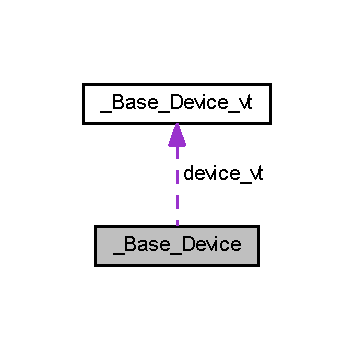
\includegraphics[width=170pt]{struct___base___device__coll__graph}
\end{center}
\end{figure}
\subsection*{Data Fields}
\begin{DoxyCompactItemize}
\item 
\hyperlink{_base___device_8h_aa8999bea473856e93a1892271b2a7d6f}{Base\-\_\-\-Device\-\_\-\-Fctn\-Table} $\ast$ \hyperlink{struct___base___device_a1a2690f94f12adfafbe276f14ffede62}{device\-\_\-vt}
\end{DoxyCompactItemize}


\subsection{Field Documentation}
\hypertarget{struct___base___device_a1a2690f94f12adfafbe276f14ffede62}{\index{\-\_\-\-Base\-\_\-\-Device@{\-\_\-\-Base\-\_\-\-Device}!device\-\_\-vt@{device\-\_\-vt}}
\index{device\-\_\-vt@{device\-\_\-vt}!_Base_Device@{\-\_\-\-Base\-\_\-\-Device}}
\subsubsection[{device\-\_\-vt}]{\setlength{\rightskip}{0pt plus 5cm}{\bf Base\-\_\-\-Device\-\_\-\-Fctn\-Table}$\ast$ \-\_\-\-Base\-\_\-\-Device\-::device\-\_\-vt}}\label{struct___base___device_a1a2690f94f12adfafbe276f14ffede62}


Referenced by sensor\-\_\-handler().



The documentation for this struct was generated from the following file\-:\begin{DoxyCompactItemize}
\item 
C\-:/\-Users/\-A\-B/\-Documents/\-Git\-Hub/\-A\-T\-M\-E\-L-\/\-A\-T\-M\-O\-S/\-A\-T\-M\-O\-S/wrapper/base-\/class/inc/\hyperlink{_base___device_8h}{Base\-\_\-\-Device.\-h}\end{DoxyCompactItemize}

\hypertarget{struct___base___device__vt}{\section{\-\_\-\-Base\-\_\-\-Device\-\_\-vt Struct Reference}
\label{struct___base___device__vt}\index{\-\_\-\-Base\-\_\-\-Device\-\_\-vt@{\-\_\-\-Base\-\_\-\-Device\-\_\-vt}}
}


{\ttfamily \#include $<$Base\-\_\-\-Device.\-h$>$}

\subsection*{Data Fields}
\begin{DoxyCompactItemize}
\item 
void($\ast$ \hyperlink{struct___base___device__vt_a01a71122bd9d5698a43fc7ea8b368c01}{V\-Tinit} )(\hyperlink{_base___device_8h_a35346bbd80cb3a10fa241ce386fb7e79}{Base\-Device} $\ast$)
\item 
int($\ast$ \hyperlink{struct___base___device__vt_a0387c5335c5e1d745a78503687fd0e51}{init} )(\hyperlink{_base___device_8h_a35346bbd80cb3a10fa241ce386fb7e79}{Base\-Device} $\ast$)
\item 
int($\ast$ \hyperlink{struct___base___device__vt_abb98aa8063ef90b5b8ac02eb060e4e68}{reset} )(\hyperlink{_base___device_8h_a35346bbd80cb3a10fa241ce386fb7e79}{Base\-Device} $\ast$)
\item 
int($\ast$ \hyperlink{struct___base___device__vt_a8471528375ff87bfc682e2baf57fa6c6}{get\-Type} )(\hyperlink{_base___device_8h_a35346bbd80cb3a10fa241ce386fb7e79}{Base\-Device} $\ast$)
\end{DoxyCompactItemize}


\subsection{Field Documentation}
\hypertarget{struct___base___device__vt_a8471528375ff87bfc682e2baf57fa6c6}{\index{\-\_\-\-Base\-\_\-\-Device\-\_\-vt@{\-\_\-\-Base\-\_\-\-Device\-\_\-vt}!get\-Type@{get\-Type}}
\index{get\-Type@{get\-Type}!_Base_Device_vt@{\-\_\-\-Base\-\_\-\-Device\-\_\-vt}}
\subsubsection[{get\-Type}]{\setlength{\rightskip}{0pt plus 5cm}int($\ast$ \-\_\-\-Base\-\_\-\-Device\-\_\-vt\-::get\-Type)({\bf Base\-Device} $\ast$)}}\label{struct___base___device__vt_a8471528375ff87bfc682e2baf57fa6c6}
\hypertarget{struct___base___device__vt_a0387c5335c5e1d745a78503687fd0e51}{\index{\-\_\-\-Base\-\_\-\-Device\-\_\-vt@{\-\_\-\-Base\-\_\-\-Device\-\_\-vt}!init@{init}}
\index{init@{init}!_Base_Device_vt@{\-\_\-\-Base\-\_\-\-Device\-\_\-vt}}
\subsubsection[{init}]{\setlength{\rightskip}{0pt plus 5cm}int($\ast$ \-\_\-\-Base\-\_\-\-Device\-\_\-vt\-::init)({\bf Base\-Device} $\ast$)}}\label{struct___base___device__vt_a0387c5335c5e1d745a78503687fd0e51}


Referenced by sensor\-\_\-handler().

\hypertarget{struct___base___device__vt_abb98aa8063ef90b5b8ac02eb060e4e68}{\index{\-\_\-\-Base\-\_\-\-Device\-\_\-vt@{\-\_\-\-Base\-\_\-\-Device\-\_\-vt}!reset@{reset}}
\index{reset@{reset}!_Base_Device_vt@{\-\_\-\-Base\-\_\-\-Device\-\_\-vt}}
\subsubsection[{reset}]{\setlength{\rightskip}{0pt plus 5cm}int($\ast$ \-\_\-\-Base\-\_\-\-Device\-\_\-vt\-::reset)({\bf Base\-Device} $\ast$)}}\label{struct___base___device__vt_abb98aa8063ef90b5b8ac02eb060e4e68}
\hypertarget{struct___base___device__vt_a01a71122bd9d5698a43fc7ea8b368c01}{\index{\-\_\-\-Base\-\_\-\-Device\-\_\-vt@{\-\_\-\-Base\-\_\-\-Device\-\_\-vt}!V\-Tinit@{V\-Tinit}}
\index{V\-Tinit@{V\-Tinit}!_Base_Device_vt@{\-\_\-\-Base\-\_\-\-Device\-\_\-vt}}
\subsubsection[{V\-Tinit}]{\setlength{\rightskip}{0pt plus 5cm}void($\ast$ \-\_\-\-Base\-\_\-\-Device\-\_\-vt\-::\-V\-Tinit)({\bf Base\-Device} $\ast$)}}\label{struct___base___device__vt_a01a71122bd9d5698a43fc7ea8b368c01}


The documentation for this struct was generated from the following file\-:\begin{DoxyCompactItemize}
\item 
C\-:/\-Users/\-A\-B/\-Documents/\-Git\-Hub/\-A\-T\-M\-E\-L-\/\-A\-T\-M\-O\-S/\-A\-T\-M\-O\-S/wrapper/base-\/class/inc/\hyperlink{_base___device_8h}{Base\-\_\-\-Device.\-h}\end{DoxyCompactItemize}

\hypertarget{struct___base___sensor}{\section{\-\_\-\-Base\-\_\-\-Sensor Struct Reference}
\label{struct___base___sensor}\index{\-\_\-\-Base\-\_\-\-Sensor@{\-\_\-\-Base\-\_\-\-Sensor}}
}


{\ttfamily \#include $<$Base\-\_\-\-Sensor.\-h$>$}



Collaboration diagram for \-\_\-\-Base\-\_\-\-Sensor\-:
\nopagebreak
\begin{figure}[H]
\begin{center}
\leavevmode
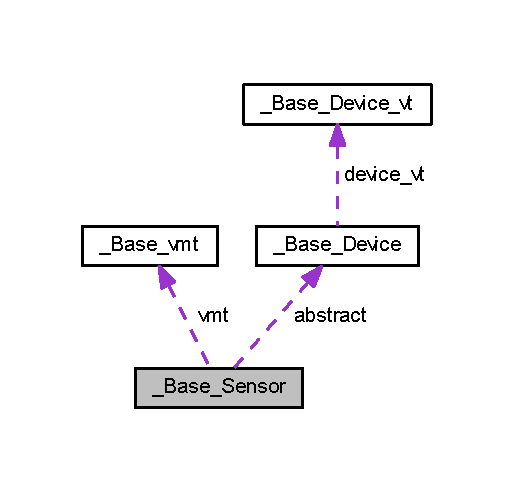
\includegraphics[width=247pt]{struct___base___sensor__coll__graph}
\end{center}
\end{figure}
\subsection*{Data Fields}
\begin{DoxyCompactItemize}
\item 
\hyperlink{_base___device_8h_a35346bbd80cb3a10fa241ce386fb7e79}{Base\-Device} \hyperlink{struct___base___sensor_ab5b10e7865be90105d136dcd5a652d54}{abstract}
\item 
int \hyperlink{struct___base___sensor_a8867289889dfcd9c796f8051e0502dda}{test\-\_\-num}
\item 
\hyperlink{_base___sensor_8h_ab5e6eb0bf1dd1e4f69e57e64004c939f}{Base\-\_\-\-Fctn\-Table} $\ast$ \hyperlink{struct___base___sensor_a45814e02e1525822b3efeae0bc06cea1}{vmt}
\end{DoxyCompactItemize}


\subsection{Field Documentation}
\hypertarget{struct___base___sensor_ab5b10e7865be90105d136dcd5a652d54}{\index{\-\_\-\-Base\-\_\-\-Sensor@{\-\_\-\-Base\-\_\-\-Sensor}!abstract@{abstract}}
\index{abstract@{abstract}!_Base_Sensor@{\-\_\-\-Base\-\_\-\-Sensor}}
\subsubsection[{abstract}]{\setlength{\rightskip}{0pt plus 5cm}{\bf Base\-Device} \-\_\-\-Base\-\_\-\-Sensor\-::abstract}}\label{struct___base___sensor_ab5b10e7865be90105d136dcd5a652d54}


Referenced by sensor\-\_\-handler().

\hypertarget{struct___base___sensor_a8867289889dfcd9c796f8051e0502dda}{\index{\-\_\-\-Base\-\_\-\-Sensor@{\-\_\-\-Base\-\_\-\-Sensor}!test\-\_\-num@{test\-\_\-num}}
\index{test\-\_\-num@{test\-\_\-num}!_Base_Sensor@{\-\_\-\-Base\-\_\-\-Sensor}}
\subsubsection[{test\-\_\-num}]{\setlength{\rightskip}{0pt plus 5cm}int \-\_\-\-Base\-\_\-\-Sensor\-::test\-\_\-num}}\label{struct___base___sensor_a8867289889dfcd9c796f8051e0502dda}


Referenced by New\-\_\-\-Base\-\_\-\-Sensor(), New\-\_\-\-B\-M\-P280\-\_\-\-Sensor(), and New\-\_\-\-My\-\_\-\-Sensor().

\hypertarget{struct___base___sensor_a45814e02e1525822b3efeae0bc06cea1}{\index{\-\_\-\-Base\-\_\-\-Sensor@{\-\_\-\-Base\-\_\-\-Sensor}!vmt@{vmt}}
\index{vmt@{vmt}!_Base_Sensor@{\-\_\-\-Base\-\_\-\-Sensor}}
\subsubsection[{vmt}]{\setlength{\rightskip}{0pt plus 5cm}{\bf Base\-\_\-\-Fctn\-Table}$\ast$ \-\_\-\-Base\-\_\-\-Sensor\-::vmt}}\label{struct___base___sensor_a45814e02e1525822b3efeae0bc06cea1}


Referenced by sensor\-\_\-handler().



The documentation for this struct was generated from the following file\-:\begin{DoxyCompactItemize}
\item 
C\-:/\-Users/\-A\-B/\-Documents/\-Git\-Hub/\-A\-T\-M\-E\-L-\/\-A\-T\-M\-O\-S/\-A\-T\-M\-O\-S/wrapper/base-\/class/inc/\hyperlink{_base___sensor_8h}{Base\-\_\-\-Sensor.\-h}\end{DoxyCompactItemize}

\hypertarget{struct___base__vmt}{\section{\-\_\-\-Base\-\_\-vmt Struct Reference}
\label{struct___base__vmt}\index{\-\_\-\-Base\-\_\-vmt@{\-\_\-\-Base\-\_\-vmt}}
}


{\ttfamily \#include $<$Base\-\_\-\-Sensor.\-h$>$}

\subsection*{Data Fields}
\begin{DoxyCompactItemize}
\item 
void($\ast$ \hyperlink{struct___base__vmt_ab21211ac2888f2e9c15ea3f7bdfe3e82}{Fctn\-Init} )(\hyperlink{_base___sensor_8h_ae91aa07b7bce6c6b463d63d8f214bb37}{Base\-Sensor} $\ast$)
\item 
int($\ast$ \hyperlink{struct___base__vmt_a4679051b7c8d66b3f4546c5e7c3d1457}{Configure} )(\hyperlink{_base___sensor_8h_ae91aa07b7bce6c6b463d63d8f214bb37}{Base\-Sensor} $\ast$)
\item 
int($\ast$ \hyperlink{struct___base__vmt_a082d37f332222c418394227f2de537f7}{Request} )(\hyperlink{_base___sensor_8h_ae91aa07b7bce6c6b463d63d8f214bb37}{Base\-Sensor} $\ast$)
\item 
int($\ast$ \hyperlink{struct___base__vmt_a3cb37486697b061a59526b2efa852ba4}{Collect} )(\hyperlink{_base___sensor_8h_ae91aa07b7bce6c6b463d63d8f214bb37}{Base\-Sensor} $\ast$)
\item 
int($\ast$ \hyperlink{struct___base__vmt_a64d04ad91e33e5f4636187057220cadd}{Error} )(\hyperlink{_base___sensor_8h_ae91aa07b7bce6c6b463d63d8f214bb37}{Base\-Sensor} $\ast$)
\end{DoxyCompactItemize}


\subsection{Field Documentation}
\hypertarget{struct___base__vmt_a3cb37486697b061a59526b2efa852ba4}{\index{\-\_\-\-Base\-\_\-vmt@{\-\_\-\-Base\-\_\-vmt}!Collect@{Collect}}
\index{Collect@{Collect}!_Base_vmt@{\-\_\-\-Base\-\_\-vmt}}
\subsubsection[{Collect}]{\setlength{\rightskip}{0pt plus 5cm}int($\ast$ \-\_\-\-Base\-\_\-vmt\-::\-Collect)({\bf Base\-Sensor} $\ast$)}}\label{struct___base__vmt_a3cb37486697b061a59526b2efa852ba4}


Referenced by sensor\-\_\-handler().

\hypertarget{struct___base__vmt_a4679051b7c8d66b3f4546c5e7c3d1457}{\index{\-\_\-\-Base\-\_\-vmt@{\-\_\-\-Base\-\_\-vmt}!Configure@{Configure}}
\index{Configure@{Configure}!_Base_vmt@{\-\_\-\-Base\-\_\-vmt}}
\subsubsection[{Configure}]{\setlength{\rightskip}{0pt plus 5cm}int($\ast$ \-\_\-\-Base\-\_\-vmt\-::\-Configure)({\bf Base\-Sensor} $\ast$)}}\label{struct___base__vmt_a4679051b7c8d66b3f4546c5e7c3d1457}
\hypertarget{struct___base__vmt_a64d04ad91e33e5f4636187057220cadd}{\index{\-\_\-\-Base\-\_\-vmt@{\-\_\-\-Base\-\_\-vmt}!Error@{Error}}
\index{Error@{Error}!_Base_vmt@{\-\_\-\-Base\-\_\-vmt}}
\subsubsection[{Error}]{\setlength{\rightskip}{0pt plus 5cm}int($\ast$ \-\_\-\-Base\-\_\-vmt\-::\-Error)({\bf Base\-Sensor} $\ast$)}}\label{struct___base__vmt_a64d04ad91e33e5f4636187057220cadd}
\hypertarget{struct___base__vmt_ab21211ac2888f2e9c15ea3f7bdfe3e82}{\index{\-\_\-\-Base\-\_\-vmt@{\-\_\-\-Base\-\_\-vmt}!Fctn\-Init@{Fctn\-Init}}
\index{Fctn\-Init@{Fctn\-Init}!_Base_vmt@{\-\_\-\-Base\-\_\-vmt}}
\subsubsection[{Fctn\-Init}]{\setlength{\rightskip}{0pt plus 5cm}void($\ast$ \-\_\-\-Base\-\_\-vmt\-::\-Fctn\-Init)({\bf Base\-Sensor} $\ast$)}}\label{struct___base__vmt_ab21211ac2888f2e9c15ea3f7bdfe3e82}
\hypertarget{struct___base__vmt_a082d37f332222c418394227f2de537f7}{\index{\-\_\-\-Base\-\_\-vmt@{\-\_\-\-Base\-\_\-vmt}!Request@{Request}}
\index{Request@{Request}!_Base_vmt@{\-\_\-\-Base\-\_\-vmt}}
\subsubsection[{Request}]{\setlength{\rightskip}{0pt plus 5cm}int($\ast$ \-\_\-\-Base\-\_\-vmt\-::\-Request)({\bf Base\-Sensor} $\ast$)}}\label{struct___base__vmt_a082d37f332222c418394227f2de537f7}


Referenced by sensor\-\_\-handler().



The documentation for this struct was generated from the following file\-:\begin{DoxyCompactItemize}
\item 
C\-:/\-Users/\-A\-B/\-Documents/\-Git\-Hub/\-A\-T\-M\-E\-L-\/\-A\-T\-M\-O\-S/\-A\-T\-M\-O\-S/wrapper/base-\/class/inc/\hyperlink{_base___sensor_8h}{Base\-\_\-\-Sensor.\-h}\end{DoxyCompactItemize}

\hypertarget{struct___b_m_p280___abstract__vmt}{\section{\-\_\-\-B\-M\-P280\-\_\-\-Abstract\-\_\-vmt Struct Reference}
\label{struct___b_m_p280___abstract__vmt}\index{\-\_\-\-B\-M\-P280\-\_\-\-Abstract\-\_\-vmt@{\-\_\-\-B\-M\-P280\-\_\-\-Abstract\-\_\-vmt}}
}


{\ttfamily \#include $<$B\-M\-P280\-\_\-\-Sensor.\-h$>$}

\subsection*{Data Fields}
\begin{DoxyCompactItemize}
\item 
void($\ast$ \hyperlink{struct___b_m_p280___abstract__vmt_a6105891d25d684f266988326151bbd67}{V\-Tinit} )(\hyperlink{_b_m_p280___sensor_8h_a60806e7544fdc94d70d1ef5937e17f28}{B\-M\-P280\-Sensor} $\ast$)
\item 
int($\ast$ \hyperlink{struct___b_m_p280___abstract__vmt_a36670528c4da556edc411db9edd3f36e}{init} )(\hyperlink{_b_m_p280___sensor_8h_a60806e7544fdc94d70d1ef5937e17f28}{B\-M\-P280\-Sensor} $\ast$)
\item 
int($\ast$ \hyperlink{struct___b_m_p280___abstract__vmt_a7c3c8f2aaf553fc88b3b14d21d0414e0}{reset} )(\hyperlink{_b_m_p280___sensor_8h_a60806e7544fdc94d70d1ef5937e17f28}{B\-M\-P280\-Sensor} $\ast$)
\item 
int($\ast$ \hyperlink{struct___b_m_p280___abstract__vmt_a64e3f581ea5deda4b375cf539b18f7d5}{get\-Type} )(\hyperlink{_b_m_p280___sensor_8h_a60806e7544fdc94d70d1ef5937e17f28}{B\-M\-P280\-Sensor} $\ast$)
\end{DoxyCompactItemize}


\subsection{Field Documentation}
\hypertarget{struct___b_m_p280___abstract__vmt_a64e3f581ea5deda4b375cf539b18f7d5}{\index{\-\_\-\-B\-M\-P280\-\_\-\-Abstract\-\_\-vmt@{\-\_\-\-B\-M\-P280\-\_\-\-Abstract\-\_\-vmt}!get\-Type@{get\-Type}}
\index{get\-Type@{get\-Type}!_BMP280_Abstract_vmt@{\-\_\-\-B\-M\-P280\-\_\-\-Abstract\-\_\-vmt}}
\subsubsection[{get\-Type}]{\setlength{\rightskip}{0pt plus 5cm}int($\ast$ \-\_\-\-B\-M\-P280\-\_\-\-Abstract\-\_\-vmt\-::get\-Type)({\bf B\-M\-P280\-Sensor} $\ast$)}}\label{struct___b_m_p280___abstract__vmt_a64e3f581ea5deda4b375cf539b18f7d5}
\hypertarget{struct___b_m_p280___abstract__vmt_a36670528c4da556edc411db9edd3f36e}{\index{\-\_\-\-B\-M\-P280\-\_\-\-Abstract\-\_\-vmt@{\-\_\-\-B\-M\-P280\-\_\-\-Abstract\-\_\-vmt}!init@{init}}
\index{init@{init}!_BMP280_Abstract_vmt@{\-\_\-\-B\-M\-P280\-\_\-\-Abstract\-\_\-vmt}}
\subsubsection[{init}]{\setlength{\rightskip}{0pt plus 5cm}int($\ast$ \-\_\-\-B\-M\-P280\-\_\-\-Abstract\-\_\-vmt\-::init)({\bf B\-M\-P280\-Sensor} $\ast$)}}\label{struct___b_m_p280___abstract__vmt_a36670528c4da556edc411db9edd3f36e}
\hypertarget{struct___b_m_p280___abstract__vmt_a7c3c8f2aaf553fc88b3b14d21d0414e0}{\index{\-\_\-\-B\-M\-P280\-\_\-\-Abstract\-\_\-vmt@{\-\_\-\-B\-M\-P280\-\_\-\-Abstract\-\_\-vmt}!reset@{reset}}
\index{reset@{reset}!_BMP280_Abstract_vmt@{\-\_\-\-B\-M\-P280\-\_\-\-Abstract\-\_\-vmt}}
\subsubsection[{reset}]{\setlength{\rightskip}{0pt plus 5cm}int($\ast$ \-\_\-\-B\-M\-P280\-\_\-\-Abstract\-\_\-vmt\-::reset)({\bf B\-M\-P280\-Sensor} $\ast$)}}\label{struct___b_m_p280___abstract__vmt_a7c3c8f2aaf553fc88b3b14d21d0414e0}
\hypertarget{struct___b_m_p280___abstract__vmt_a6105891d25d684f266988326151bbd67}{\index{\-\_\-\-B\-M\-P280\-\_\-\-Abstract\-\_\-vmt@{\-\_\-\-B\-M\-P280\-\_\-\-Abstract\-\_\-vmt}!V\-Tinit@{V\-Tinit}}
\index{V\-Tinit@{V\-Tinit}!_BMP280_Abstract_vmt@{\-\_\-\-B\-M\-P280\-\_\-\-Abstract\-\_\-vmt}}
\subsubsection[{V\-Tinit}]{\setlength{\rightskip}{0pt plus 5cm}void($\ast$ \-\_\-\-B\-M\-P280\-\_\-\-Abstract\-\_\-vmt\-::\-V\-Tinit)({\bf B\-M\-P280\-Sensor} $\ast$)}}\label{struct___b_m_p280___abstract__vmt_a6105891d25d684f266988326151bbd67}


The documentation for this struct was generated from the following file\-:\begin{DoxyCompactItemize}
\item 
C\-:/\-Users/\-A\-B/\-Documents/\-Git\-Hub/\-A\-T\-M\-E\-L-\/\-A\-T\-M\-O\-S/\-A\-T\-M\-O\-S/wrapper/sensor/inc/\hyperlink{_b_m_p280___sensor_8h}{B\-M\-P280\-\_\-\-Sensor.\-h}\end{DoxyCompactItemize}

\hypertarget{struct___b_m_p280___sensor}{\section{\-\_\-\-B\-M\-P280\-\_\-\-Sensor Struct Reference}
\label{struct___b_m_p280___sensor}\index{\-\_\-\-B\-M\-P280\-\_\-\-Sensor@{\-\_\-\-B\-M\-P280\-\_\-\-Sensor}}
}


{\ttfamily \#include $<$B\-M\-P280\-\_\-\-Sensor.\-h$>$}



Collaboration diagram for \-\_\-\-B\-M\-P280\-\_\-\-Sensor\-:
\nopagebreak
\begin{figure}[H]
\begin{center}
\leavevmode
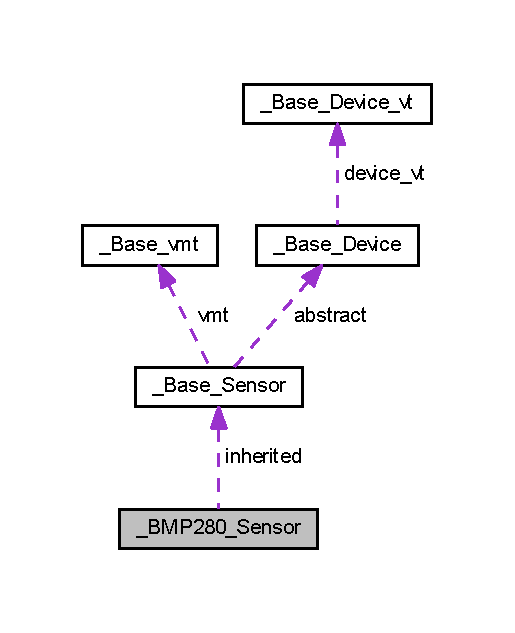
\includegraphics[width=247pt]{struct___b_m_p280___sensor__coll__graph}
\end{center}
\end{figure}
\subsection*{Data Fields}
\begin{DoxyCompactItemize}
\item 
\hyperlink{_base___sensor_8h_ae91aa07b7bce6c6b463d63d8f214bb37}{Base\-Sensor} \hyperlink{struct___b_m_p280___sensor_a35781d57029c477ad5c22cdbcce55e71}{inherited}
\end{DoxyCompactItemize}


\subsection{Field Documentation}
\hypertarget{struct___b_m_p280___sensor_a35781d57029c477ad5c22cdbcce55e71}{\index{\-\_\-\-B\-M\-P280\-\_\-\-Sensor@{\-\_\-\-B\-M\-P280\-\_\-\-Sensor}!inherited@{inherited}}
\index{inherited@{inherited}!_BMP280_Sensor@{\-\_\-\-B\-M\-P280\-\_\-\-Sensor}}
\subsubsection[{inherited}]{\setlength{\rightskip}{0pt plus 5cm}{\bf Base\-Sensor} \-\_\-\-B\-M\-P280\-\_\-\-Sensor\-::inherited}}\label{struct___b_m_p280___sensor_a35781d57029c477ad5c22cdbcce55e71}


Referenced by New\-\_\-\-B\-M\-P280\-\_\-\-Sensor().



The documentation for this struct was generated from the following file\-:\begin{DoxyCompactItemize}
\item 
C\-:/\-Users/\-A\-B/\-Documents/\-Git\-Hub/\-A\-T\-M\-E\-L-\/\-A\-T\-M\-O\-S/\-A\-T\-M\-O\-S/wrapper/sensor/inc/\hyperlink{_b_m_p280___sensor_8h}{B\-M\-P280\-\_\-\-Sensor.\-h}\end{DoxyCompactItemize}

\hypertarget{struct___b_m_p280__vmt}{\section{\-\_\-\-B\-M\-P280\-\_\-vmt Struct Reference}
\label{struct___b_m_p280__vmt}\index{\-\_\-\-B\-M\-P280\-\_\-vmt@{\-\_\-\-B\-M\-P280\-\_\-vmt}}
}


{\ttfamily \#include $<$B\-M\-P280\-\_\-\-Sensor.\-h$>$}

\subsection*{Data Fields}
\begin{DoxyCompactItemize}
\item 
void($\ast$ \hyperlink{struct___b_m_p280__vmt_a56cb4f192918dab19f6594f332cd8c51}{Fctn\-Init} )(\hyperlink{_b_m_p280___sensor_8h_a60806e7544fdc94d70d1ef5937e17f28}{B\-M\-P280\-Sensor} $\ast$)
\item 
int($\ast$ \hyperlink{struct___b_m_p280__vmt_a02c800133b0696a925cc7cab20cf385f}{Configure} )(\hyperlink{_b_m_p280___sensor_8h_a60806e7544fdc94d70d1ef5937e17f28}{B\-M\-P280\-Sensor} $\ast$)
\item 
int($\ast$ \hyperlink{struct___b_m_p280__vmt_a92b083c30e4c2517137943ce6e787547}{Request} )(\hyperlink{_b_m_p280___sensor_8h_a60806e7544fdc94d70d1ef5937e17f28}{B\-M\-P280\-Sensor} $\ast$)
\item 
int($\ast$ \hyperlink{struct___b_m_p280__vmt_a807519b51b953f4be7be6778a53905dc}{Collect} )(\hyperlink{_b_m_p280___sensor_8h_a60806e7544fdc94d70d1ef5937e17f28}{B\-M\-P280\-Sensor} $\ast$)
\item 
int($\ast$ \hyperlink{struct___b_m_p280__vmt_aa31c53475ba0d8d65d5c3cc56753f6f0}{Error} )(\hyperlink{_b_m_p280___sensor_8h_a60806e7544fdc94d70d1ef5937e17f28}{B\-M\-P280\-Sensor} $\ast$)
\end{DoxyCompactItemize}


\subsection{Field Documentation}
\hypertarget{struct___b_m_p280__vmt_a807519b51b953f4be7be6778a53905dc}{\index{\-\_\-\-B\-M\-P280\-\_\-vmt@{\-\_\-\-B\-M\-P280\-\_\-vmt}!Collect@{Collect}}
\index{Collect@{Collect}!_BMP280_vmt@{\-\_\-\-B\-M\-P280\-\_\-vmt}}
\subsubsection[{Collect}]{\setlength{\rightskip}{0pt plus 5cm}int($\ast$ \-\_\-\-B\-M\-P280\-\_\-vmt\-::\-Collect)({\bf B\-M\-P280\-Sensor} $\ast$)}}\label{struct___b_m_p280__vmt_a807519b51b953f4be7be6778a53905dc}
\hypertarget{struct___b_m_p280__vmt_a02c800133b0696a925cc7cab20cf385f}{\index{\-\_\-\-B\-M\-P280\-\_\-vmt@{\-\_\-\-B\-M\-P280\-\_\-vmt}!Configure@{Configure}}
\index{Configure@{Configure}!_BMP280_vmt@{\-\_\-\-B\-M\-P280\-\_\-vmt}}
\subsubsection[{Configure}]{\setlength{\rightskip}{0pt plus 5cm}int($\ast$ \-\_\-\-B\-M\-P280\-\_\-vmt\-::\-Configure)({\bf B\-M\-P280\-Sensor} $\ast$)}}\label{struct___b_m_p280__vmt_a02c800133b0696a925cc7cab20cf385f}
\hypertarget{struct___b_m_p280__vmt_aa31c53475ba0d8d65d5c3cc56753f6f0}{\index{\-\_\-\-B\-M\-P280\-\_\-vmt@{\-\_\-\-B\-M\-P280\-\_\-vmt}!Error@{Error}}
\index{Error@{Error}!_BMP280_vmt@{\-\_\-\-B\-M\-P280\-\_\-vmt}}
\subsubsection[{Error}]{\setlength{\rightskip}{0pt plus 5cm}int($\ast$ \-\_\-\-B\-M\-P280\-\_\-vmt\-::\-Error)({\bf B\-M\-P280\-Sensor} $\ast$)}}\label{struct___b_m_p280__vmt_aa31c53475ba0d8d65d5c3cc56753f6f0}
\hypertarget{struct___b_m_p280__vmt_a56cb4f192918dab19f6594f332cd8c51}{\index{\-\_\-\-B\-M\-P280\-\_\-vmt@{\-\_\-\-B\-M\-P280\-\_\-vmt}!Fctn\-Init@{Fctn\-Init}}
\index{Fctn\-Init@{Fctn\-Init}!_BMP280_vmt@{\-\_\-\-B\-M\-P280\-\_\-vmt}}
\subsubsection[{Fctn\-Init}]{\setlength{\rightskip}{0pt plus 5cm}void($\ast$ \-\_\-\-B\-M\-P280\-\_\-vmt\-::\-Fctn\-Init)({\bf B\-M\-P280\-Sensor} $\ast$)}}\label{struct___b_m_p280__vmt_a56cb4f192918dab19f6594f332cd8c51}
\hypertarget{struct___b_m_p280__vmt_a92b083c30e4c2517137943ce6e787547}{\index{\-\_\-\-B\-M\-P280\-\_\-vmt@{\-\_\-\-B\-M\-P280\-\_\-vmt}!Request@{Request}}
\index{Request@{Request}!_BMP280_vmt@{\-\_\-\-B\-M\-P280\-\_\-vmt}}
\subsubsection[{Request}]{\setlength{\rightskip}{0pt plus 5cm}int($\ast$ \-\_\-\-B\-M\-P280\-\_\-vmt\-::\-Request)({\bf B\-M\-P280\-Sensor} $\ast$)}}\label{struct___b_m_p280__vmt_a92b083c30e4c2517137943ce6e787547}


The documentation for this struct was generated from the following file\-:\begin{DoxyCompactItemize}
\item 
C\-:/\-Users/\-A\-B/\-Documents/\-Git\-Hub/\-A\-T\-M\-E\-L-\/\-A\-T\-M\-O\-S/\-A\-T\-M\-O\-S/wrapper/sensor/inc/\hyperlink{_b_m_p280___sensor_8h}{B\-M\-P280\-\_\-\-Sensor.\-h}\end{DoxyCompactItemize}

\hypertarget{struct__llp}{\section{\-\_\-llp Struct Reference}
\label{struct__llp}\index{\-\_\-llp@{\-\_\-llp}}
}


{\ttfamily \#include $<$llist.\-h$>$}

\subsection*{Data Fields}
\begin{DoxyCompactItemize}
\item 
\hyperlink{struct__llp_aeb980327ef185ef35b1b028d541463cf}{L\-L\-\_\-\-P\-T\-R\-S}
\end{DoxyCompactItemize}


\subsection{Field Documentation}
\hypertarget{struct__llp_aeb980327ef185ef35b1b028d541463cf}{\index{\-\_\-llp@{\-\_\-llp}!L\-L\-\_\-\-P\-T\-R\-S@{L\-L\-\_\-\-P\-T\-R\-S}}
\index{L\-L\-\_\-\-P\-T\-R\-S@{L\-L\-\_\-\-P\-T\-R\-S}!_llp@{\-\_\-llp}}
\subsubsection[{L\-L\-\_\-\-P\-T\-R\-S}]{\setlength{\rightskip}{0pt plus 5cm}\-\_\-llp\-::\-L\-L\-\_\-\-P\-T\-R\-S}}\label{struct__llp_aeb980327ef185ef35b1b028d541463cf}


The documentation for this struct was generated from the following file\-:\begin{DoxyCompactItemize}
\item 
C\-:/\-Users/\-A\-B/\-Documents/\-Git\-Hub/\-A\-T\-M\-E\-L-\/\-A\-T\-M\-O\-S/\-A\-T\-M\-O\-S/utilities/inc/\hyperlink{llist_8h}{llist.\-h}\end{DoxyCompactItemize}

\hypertarget{struct___my___abstract__vmt}{\section{\-\_\-\-My\-\_\-\-Abstract\-\_\-vmt Struct Reference}
\label{struct___my___abstract__vmt}\index{\-\_\-\-My\-\_\-\-Abstract\-\_\-vmt@{\-\_\-\-My\-\_\-\-Abstract\-\_\-vmt}}
}


{\ttfamily \#include $<$My\-\_\-\-Sensor.\-h$>$}

\subsection*{Data Fields}
\begin{DoxyCompactItemize}
\item 
void($\ast$ \hyperlink{struct___my___abstract__vmt_a2c999bc46b0745aa624051ac48d3347e}{V\-Tinit} )(\hyperlink{_my___sensor_8h_aec3fece1ce83f3dd577aa3228199813f}{My\-Sensor} $\ast$)
\item 
int($\ast$ \hyperlink{struct___my___abstract__vmt_a8f309bfdf6a70191aaa8c53a1ce55d83}{init} )(\hyperlink{_my___sensor_8h_aec3fece1ce83f3dd577aa3228199813f}{My\-Sensor} $\ast$)
\item 
int($\ast$ \hyperlink{struct___my___abstract__vmt_a825ffb364bcce5bb1ebfec3a61fd399c}{reset} )(\hyperlink{_my___sensor_8h_aec3fece1ce83f3dd577aa3228199813f}{My\-Sensor} $\ast$)
\item 
int($\ast$ \hyperlink{struct___my___abstract__vmt_afa39974172b5cb02e5bb29c28628fde7}{get\-Type} )(\hyperlink{_my___sensor_8h_aec3fece1ce83f3dd577aa3228199813f}{My\-Sensor} $\ast$)
\end{DoxyCompactItemize}


\subsection{Field Documentation}
\hypertarget{struct___my___abstract__vmt_afa39974172b5cb02e5bb29c28628fde7}{\index{\-\_\-\-My\-\_\-\-Abstract\-\_\-vmt@{\-\_\-\-My\-\_\-\-Abstract\-\_\-vmt}!get\-Type@{get\-Type}}
\index{get\-Type@{get\-Type}!_My_Abstract_vmt@{\-\_\-\-My\-\_\-\-Abstract\-\_\-vmt}}
\subsubsection[{get\-Type}]{\setlength{\rightskip}{0pt plus 5cm}int($\ast$ \-\_\-\-My\-\_\-\-Abstract\-\_\-vmt\-::get\-Type)({\bf My\-Sensor} $\ast$)}}\label{struct___my___abstract__vmt_afa39974172b5cb02e5bb29c28628fde7}
\hypertarget{struct___my___abstract__vmt_a8f309bfdf6a70191aaa8c53a1ce55d83}{\index{\-\_\-\-My\-\_\-\-Abstract\-\_\-vmt@{\-\_\-\-My\-\_\-\-Abstract\-\_\-vmt}!init@{init}}
\index{init@{init}!_My_Abstract_vmt@{\-\_\-\-My\-\_\-\-Abstract\-\_\-vmt}}
\subsubsection[{init}]{\setlength{\rightskip}{0pt plus 5cm}int($\ast$ \-\_\-\-My\-\_\-\-Abstract\-\_\-vmt\-::init)({\bf My\-Sensor} $\ast$)}}\label{struct___my___abstract__vmt_a8f309bfdf6a70191aaa8c53a1ce55d83}
\hypertarget{struct___my___abstract__vmt_a825ffb364bcce5bb1ebfec3a61fd399c}{\index{\-\_\-\-My\-\_\-\-Abstract\-\_\-vmt@{\-\_\-\-My\-\_\-\-Abstract\-\_\-vmt}!reset@{reset}}
\index{reset@{reset}!_My_Abstract_vmt@{\-\_\-\-My\-\_\-\-Abstract\-\_\-vmt}}
\subsubsection[{reset}]{\setlength{\rightskip}{0pt plus 5cm}int($\ast$ \-\_\-\-My\-\_\-\-Abstract\-\_\-vmt\-::reset)({\bf My\-Sensor} $\ast$)}}\label{struct___my___abstract__vmt_a825ffb364bcce5bb1ebfec3a61fd399c}
\hypertarget{struct___my___abstract__vmt_a2c999bc46b0745aa624051ac48d3347e}{\index{\-\_\-\-My\-\_\-\-Abstract\-\_\-vmt@{\-\_\-\-My\-\_\-\-Abstract\-\_\-vmt}!V\-Tinit@{V\-Tinit}}
\index{V\-Tinit@{V\-Tinit}!_My_Abstract_vmt@{\-\_\-\-My\-\_\-\-Abstract\-\_\-vmt}}
\subsubsection[{V\-Tinit}]{\setlength{\rightskip}{0pt plus 5cm}void($\ast$ \-\_\-\-My\-\_\-\-Abstract\-\_\-vmt\-::\-V\-Tinit)({\bf My\-Sensor} $\ast$)}}\label{struct___my___abstract__vmt_a2c999bc46b0745aa624051ac48d3347e}


The documentation for this struct was generated from the following file\-:\begin{DoxyCompactItemize}
\item 
C\-:/\-Users/\-A\-B/\-Documents/\-Git\-Hub/\-A\-T\-M\-E\-L-\/\-A\-T\-M\-O\-S/\-A\-T\-M\-O\-S/wrapper/sensor/inc/\hyperlink{_my___sensor_8h}{My\-\_\-\-Sensor.\-h}\end{DoxyCompactItemize}

\hypertarget{struct___my___sensor}{\section{\-\_\-\-My\-\_\-\-Sensor Struct Reference}
\label{struct___my___sensor}\index{\-\_\-\-My\-\_\-\-Sensor@{\-\_\-\-My\-\_\-\-Sensor}}
}


{\ttfamily \#include $<$My\-\_\-\-Sensor.\-h$>$}



Collaboration diagram for \-\_\-\-My\-\_\-\-Sensor\-:
\nopagebreak
\begin{figure}[H]
\begin{center}
\leavevmode
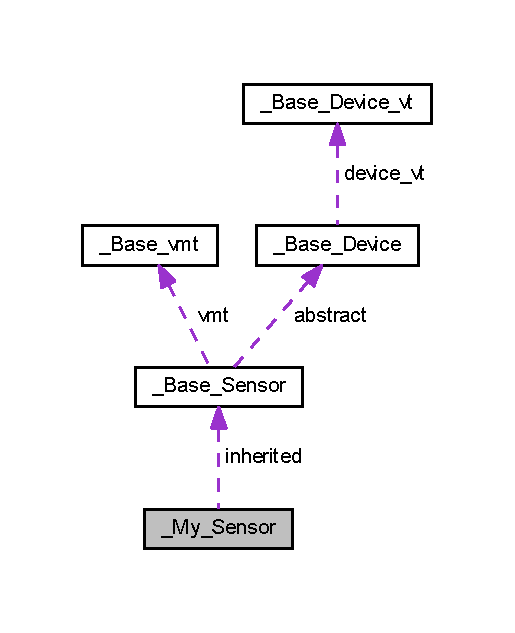
\includegraphics[width=247pt]{struct___my___sensor__coll__graph}
\end{center}
\end{figure}
\subsection*{Data Fields}
\begin{DoxyCompactItemize}
\item 
\hyperlink{_base___sensor_8h_ae91aa07b7bce6c6b463d63d8f214bb37}{Base\-Sensor} \hyperlink{struct___my___sensor_abcbafe15ac0db03286d064456a15e2ad}{inherited}
\end{DoxyCompactItemize}


\subsection{Field Documentation}
\hypertarget{struct___my___sensor_abcbafe15ac0db03286d064456a15e2ad}{\index{\-\_\-\-My\-\_\-\-Sensor@{\-\_\-\-My\-\_\-\-Sensor}!inherited@{inherited}}
\index{inherited@{inherited}!_My_Sensor@{\-\_\-\-My\-\_\-\-Sensor}}
\subsubsection[{inherited}]{\setlength{\rightskip}{0pt plus 5cm}{\bf Base\-Sensor} \-\_\-\-My\-\_\-\-Sensor\-::inherited}}\label{struct___my___sensor_abcbafe15ac0db03286d064456a15e2ad}


Referenced by New\-\_\-\-My\-\_\-\-Sensor().



The documentation for this struct was generated from the following file\-:\begin{DoxyCompactItemize}
\item 
C\-:/\-Users/\-A\-B/\-Documents/\-Git\-Hub/\-A\-T\-M\-E\-L-\/\-A\-T\-M\-O\-S/\-A\-T\-M\-O\-S/wrapper/sensor/inc/\hyperlink{_my___sensor_8h}{My\-\_\-\-Sensor.\-h}\end{DoxyCompactItemize}

\hypertarget{struct___my__vmt}{\section{\-\_\-\-My\-\_\-vmt Struct Reference}
\label{struct___my__vmt}\index{\-\_\-\-My\-\_\-vmt@{\-\_\-\-My\-\_\-vmt}}
}


{\ttfamily \#include $<$My\-\_\-\-Sensor.\-h$>$}

\subsection*{Data Fields}
\begin{DoxyCompactItemize}
\item 
void($\ast$ \hyperlink{struct___my__vmt_a43f9f9d8e0c1d315836bb28612d18bee}{Fctn\-Init} )(\hyperlink{_my___sensor_8h_aec3fece1ce83f3dd577aa3228199813f}{My\-Sensor} $\ast$)
\item 
int($\ast$ \hyperlink{struct___my__vmt_ae66aa549ba7b48620e02989da56da5a5}{Configure} )(\hyperlink{_my___sensor_8h_aec3fece1ce83f3dd577aa3228199813f}{My\-Sensor} $\ast$)
\item 
int($\ast$ \hyperlink{struct___my__vmt_a2d1dad94e54417934087cf76a8e32245}{Request} )(\hyperlink{_my___sensor_8h_aec3fece1ce83f3dd577aa3228199813f}{My\-Sensor} $\ast$)
\item 
int($\ast$ \hyperlink{struct___my__vmt_a886b58b662a06712e400abefd0d5d677}{Collect} )(\hyperlink{_my___sensor_8h_aec3fece1ce83f3dd577aa3228199813f}{My\-Sensor} $\ast$)
\item 
int($\ast$ \hyperlink{struct___my__vmt_a7fd6e75b116d4744299ececa6286d274}{Error} )(\hyperlink{_my___sensor_8h_aec3fece1ce83f3dd577aa3228199813f}{My\-Sensor} $\ast$)
\end{DoxyCompactItemize}


\subsection{Field Documentation}
\hypertarget{struct___my__vmt_a886b58b662a06712e400abefd0d5d677}{\index{\-\_\-\-My\-\_\-vmt@{\-\_\-\-My\-\_\-vmt}!Collect@{Collect}}
\index{Collect@{Collect}!_My_vmt@{\-\_\-\-My\-\_\-vmt}}
\subsubsection[{Collect}]{\setlength{\rightskip}{0pt plus 5cm}int($\ast$ \-\_\-\-My\-\_\-vmt\-::\-Collect)({\bf My\-Sensor} $\ast$)}}\label{struct___my__vmt_a886b58b662a06712e400abefd0d5d677}
\hypertarget{struct___my__vmt_ae66aa549ba7b48620e02989da56da5a5}{\index{\-\_\-\-My\-\_\-vmt@{\-\_\-\-My\-\_\-vmt}!Configure@{Configure}}
\index{Configure@{Configure}!_My_vmt@{\-\_\-\-My\-\_\-vmt}}
\subsubsection[{Configure}]{\setlength{\rightskip}{0pt plus 5cm}int($\ast$ \-\_\-\-My\-\_\-vmt\-::\-Configure)({\bf My\-Sensor} $\ast$)}}\label{struct___my__vmt_ae66aa549ba7b48620e02989da56da5a5}
\hypertarget{struct___my__vmt_a7fd6e75b116d4744299ececa6286d274}{\index{\-\_\-\-My\-\_\-vmt@{\-\_\-\-My\-\_\-vmt}!Error@{Error}}
\index{Error@{Error}!_My_vmt@{\-\_\-\-My\-\_\-vmt}}
\subsubsection[{Error}]{\setlength{\rightskip}{0pt plus 5cm}int($\ast$ \-\_\-\-My\-\_\-vmt\-::\-Error)({\bf My\-Sensor} $\ast$)}}\label{struct___my__vmt_a7fd6e75b116d4744299ececa6286d274}
\hypertarget{struct___my__vmt_a43f9f9d8e0c1d315836bb28612d18bee}{\index{\-\_\-\-My\-\_\-vmt@{\-\_\-\-My\-\_\-vmt}!Fctn\-Init@{Fctn\-Init}}
\index{Fctn\-Init@{Fctn\-Init}!_My_vmt@{\-\_\-\-My\-\_\-vmt}}
\subsubsection[{Fctn\-Init}]{\setlength{\rightskip}{0pt plus 5cm}void($\ast$ \-\_\-\-My\-\_\-vmt\-::\-Fctn\-Init)({\bf My\-Sensor} $\ast$)}}\label{struct___my__vmt_a43f9f9d8e0c1d315836bb28612d18bee}
\hypertarget{struct___my__vmt_a2d1dad94e54417934087cf76a8e32245}{\index{\-\_\-\-My\-\_\-vmt@{\-\_\-\-My\-\_\-vmt}!Request@{Request}}
\index{Request@{Request}!_My_vmt@{\-\_\-\-My\-\_\-vmt}}
\subsubsection[{Request}]{\setlength{\rightskip}{0pt plus 5cm}int($\ast$ \-\_\-\-My\-\_\-vmt\-::\-Request)({\bf My\-Sensor} $\ast$)}}\label{struct___my__vmt_a2d1dad94e54417934087cf76a8e32245}


The documentation for this struct was generated from the following file\-:\begin{DoxyCompactItemize}
\item 
C\-:/\-Users/\-A\-B/\-Documents/\-Git\-Hub/\-A\-T\-M\-E\-L-\/\-A\-T\-M\-O\-S/\-A\-T\-M\-O\-S/wrapper/sensor/inc/\hyperlink{_my___sensor_8h}{My\-\_\-\-Sensor.\-h}\end{DoxyCompactItemize}

\hypertarget{struct_data_unit}{\section{Data\-Unit Struct Reference}
\label{struct_data_unit}\index{Data\-Unit@{Data\-Unit}}
}


{\ttfamily \#include $<$data\-\_\-unit.\-h$>$}



Collaboration diagram for Data\-Unit\-:
\nopagebreak
\begin{figure}[H]
\begin{center}
\leavevmode
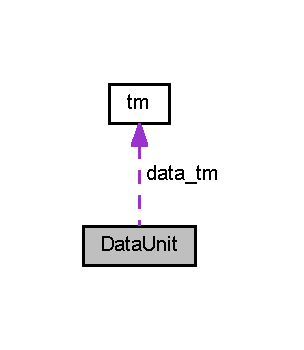
\includegraphics[width=146pt]{struct_data_unit__coll__graph}
\end{center}
\end{figure}
\subsection*{Data Fields}
\begin{DoxyCompactItemize}
\item 
double \hyperlink{struct_data_unit_a9f22b6f4d67d8bfb0e247cd51a3e1a09}{data} \mbox{[}\hyperlink{common_8h_af796c1f43785b427dbf1ede1da7af498}{M\-A\-X\-\_\-\-N\-U\-M\-\_\-\-D\-A\-T\-A}\mbox{]}
\item 
\hyperlink{structtm}{tm} \hyperlink{struct_data_unit_a1f660834a81d15ce3ec54275f7de1861}{data\-\_\-tm}
\end{DoxyCompactItemize}


\subsection{Field Documentation}
\hypertarget{struct_data_unit_a9f22b6f4d67d8bfb0e247cd51a3e1a09}{\index{Data\-Unit@{Data\-Unit}!data@{data}}
\index{data@{data}!DataUnit@{Data\-Unit}}
\subsubsection[{data}]{\setlength{\rightskip}{0pt plus 5cm}double Data\-Unit\-::data\mbox{[}{\bf M\-A\-X\-\_\-\-N\-U\-M\-\_\-\-D\-A\-T\-A}\mbox{]}}}\label{struct_data_unit_a9f22b6f4d67d8bfb0e247cd51a3e1a09}
\hypertarget{struct_data_unit_a1f660834a81d15ce3ec54275f7de1861}{\index{Data\-Unit@{Data\-Unit}!data\-\_\-tm@{data\-\_\-tm}}
\index{data\-\_\-tm@{data\-\_\-tm}!DataUnit@{Data\-Unit}}
\subsubsection[{data\-\_\-tm}]{\setlength{\rightskip}{0pt plus 5cm}{\bf tm} Data\-Unit\-::data\-\_\-tm}}\label{struct_data_unit_a1f660834a81d15ce3ec54275f7de1861}


The documentation for this struct was generated from the following file\-:\begin{DoxyCompactItemize}
\item 
C\-:/\-Users/\-A\-B/\-Documents/\-Git\-Hub/\-A\-T\-M\-E\-L-\/\-A\-T\-M\-O\-S/\-A\-T\-M\-O\-S/utilities/inc/\hyperlink{data__unit_8h}{data\-\_\-unit.\-h}\end{DoxyCompactItemize}

\hypertarget{structevent}{\section{event Struct Reference}
\label{structevent}\index{event@{event}}
}


A container struct to hold device/sensor pointer and corresponding timeout info.  




{\ttfamily \#include $<$event.\-h$>$}



Collaboration diagram for event\-:
\nopagebreak
\begin{figure}[H]
\begin{center}
\leavevmode
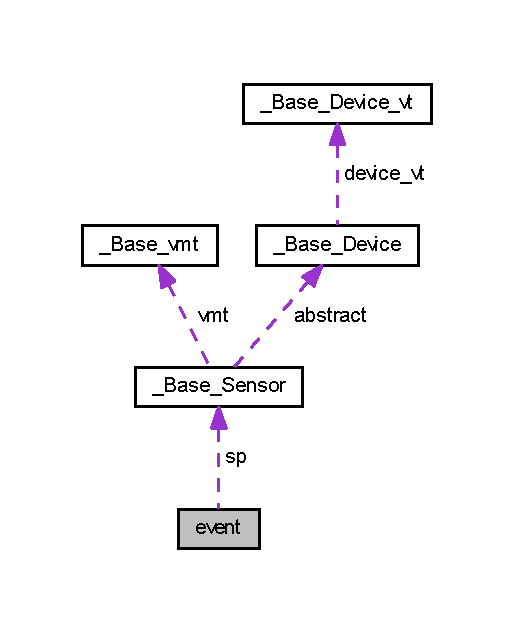
\includegraphics[width=247pt]{structevent__coll__graph}
\end{center}
\end{figure}
\subsection*{Data Fields}
\begin{DoxyCompactItemize}
\item 
\hyperlink{structevent_a994b32d8396bd5e998df0956908ec79d}{L\-L\-\_\-\-P\-T\-R\-S}
\item 
int \hyperlink{structevent_a0da07c7694fd4b1e45c1cb5d65fb962b}{timeout}
\begin{DoxyCompactList}\small\item\em next timeout value in ms. \end{DoxyCompactList}\item 
int \hyperlink{structevent_a2792fb8dafb449872de1213c65c89474}{repeat\-\_\-interval}
\begin{DoxyCompactList}\small\item\em the repeat period of the event in ms. 0 means no repeatence. \end{DoxyCompactList}\item 
int \hyperlink{structevent_a956c9abffd9faff3f90040f464d2423e}{borrow\-\_\-timeout}
\item 
\hyperlink{_base___sensor_8h_ae91aa07b7bce6c6b463d63d8f214bb37}{Base\-Sensor} $\ast$ \hyperlink{structevent_a64304637019072f9322aef7ecf4a7c00}{sp}
\item 
int \hyperlink{structevent_aa6d0cb63c9eb781957c1db988d71d12f}{info}
\item 
enum \hyperlink{common_8h_a0c10345a5a61ea917f59a0437ad481a0}{Device\-State} \hyperlink{structevent_ad434572c03708c933947eb50f4bb5403}{cur\-\_\-state}
\item 
int($\ast$ \hyperlink{structevent_add5b35b1741734964a494b100224aaea}{run} )(struct \hyperlink{structevent}{event} $\ast$)
\end{DoxyCompactItemize}


\subsection{Detailed Description}
A container struct to hold device/sensor pointer and corresponding timeout info. 

\subsection{Field Documentation}
\hypertarget{structevent_a956c9abffd9faff3f90040f464d2423e}{\index{event@{event}!borrow\-\_\-timeout@{borrow\-\_\-timeout}}
\index{borrow\-\_\-timeout@{borrow\-\_\-timeout}!event@{event}}
\subsubsection[{borrow\-\_\-timeout}]{\setlength{\rightskip}{0pt plus 5cm}int event\-::borrow\-\_\-timeout}}\label{structevent_a956c9abffd9faff3f90040f464d2423e}


Referenced by handle\-\_\-timeoutq\-\_\-event(), load\-\_\-new\-\_\-sensor(), and sensor\-\_\-handler().

\hypertarget{structevent_ad434572c03708c933947eb50f4bb5403}{\index{event@{event}!cur\-\_\-state@{cur\-\_\-state}}
\index{cur\-\_\-state@{cur\-\_\-state}!event@{event}}
\subsubsection[{cur\-\_\-state}]{\setlength{\rightskip}{0pt plus 5cm}enum {\bf Device\-State} event\-::cur\-\_\-state}}\label{structevent_ad434572c03708c933947eb50f4bb5403}


Referenced by device\-\_\-handler(), load\-\_\-new\-\_\-sensor(), and sensor\-\_\-handler().

\hypertarget{structevent_aa6d0cb63c9eb781957c1db988d71d12f}{\index{event@{event}!info@{info}}
\index{info@{info}!event@{event}}
\subsubsection[{info}]{\setlength{\rightskip}{0pt plus 5cm}int event\-::info}}\label{structevent_aa6d0cb63c9eb781957c1db988d71d12f}


Referenced by load\-\_\-new\-\_\-sensor().

\hypertarget{structevent_a994b32d8396bd5e998df0956908ec79d}{\index{event@{event}!L\-L\-\_\-\-P\-T\-R\-S@{L\-L\-\_\-\-P\-T\-R\-S}}
\index{L\-L\-\_\-\-P\-T\-R\-S@{L\-L\-\_\-\-P\-T\-R\-S}!event@{event}}
\subsubsection[{L\-L\-\_\-\-P\-T\-R\-S}]{\setlength{\rightskip}{0pt plus 5cm}event\-::\-L\-L\-\_\-\-P\-T\-R\-S}}\label{structevent_a994b32d8396bd5e998df0956908ec79d}
\hypertarget{structevent_a2792fb8dafb449872de1213c65c89474}{\index{event@{event}!repeat\-\_\-interval@{repeat\-\_\-interval}}
\index{repeat\-\_\-interval@{repeat\-\_\-interval}!event@{event}}
\subsubsection[{repeat\-\_\-interval}]{\setlength{\rightskip}{0pt plus 5cm}int event\-::repeat\-\_\-interval}}\label{structevent_a2792fb8dafb449872de1213c65c89474}


the repeat period of the event in ms. 0 means no repeatence. 



Referenced by handle\-\_\-timeoutq\-\_\-event(), and load\-\_\-new\-\_\-sensor().

\hypertarget{structevent_add5b35b1741734964a494b100224aaea}{\index{event@{event}!run@{run}}
\index{run@{run}!event@{event}}
\subsubsection[{run}]{\setlength{\rightskip}{0pt plus 5cm}int($\ast$  event\-::run)(struct {\bf event} $\ast$)}}\label{structevent_add5b35b1741734964a494b100224aaea}


Referenced by handle\-\_\-timeoutq\-\_\-event(), and load\-\_\-new\-\_\-sensor().

\hypertarget{structevent_a64304637019072f9322aef7ecf4a7c00}{\index{event@{event}!sp@{sp}}
\index{sp@{sp}!event@{event}}
\subsubsection[{sp}]{\setlength{\rightskip}{0pt plus 5cm}{\bf Base\-Sensor}$\ast$ event\-::sp}}\label{structevent_a64304637019072f9322aef7ecf4a7c00}


Referenced by handle\-\_\-timeoutq\-\_\-event(), load\-\_\-new\-\_\-sensor(), sensor\-\_\-handler(), and store\-Data\-\_\-handler().

\hypertarget{structevent_a0da07c7694fd4b1e45c1cb5d65fb962b}{\index{event@{event}!timeout@{timeout}}
\index{timeout@{timeout}!event@{event}}
\subsubsection[{timeout}]{\setlength{\rightskip}{0pt plus 5cm}int event\-::timeout}}\label{structevent_a0da07c7694fd4b1e45c1cb5d65fb962b}


next timeout value in ms. 



Referenced by get\-\_\-next\-\_\-interval(), handle\-\_\-timeoutq\-\_\-event(), insert\-\_\-timeoutq\-\_\-event(), load\-\_\-new\-\_\-sensor(), and sensor\-\_\-handler().



The documentation for this struct was generated from the following file\-:\begin{DoxyCompactItemize}
\item 
C\-:/\-Users/\-A\-B/\-Documents/\-Git\-Hub/\-A\-T\-M\-E\-L-\/\-A\-T\-M\-O\-S/\-A\-T\-M\-O\-S/scheduler/inc/\hyperlink{event_8h}{event.\-h}\end{DoxyCompactItemize}

\hypertarget{struct_n_w_k___data_ind__t}{\section{N\-W\-K\-\_\-\-Data\-Ind\-\_\-t Struct Reference}
\label{struct_n_w_k___data_ind__t}\index{N\-W\-K\-\_\-\-Data\-Ind\-\_\-t@{N\-W\-K\-\_\-\-Data\-Ind\-\_\-t}}
}


{\ttfamily \#include $<$nwk\-Rx.\-h$>$}

\subsection*{Data Fields}
\begin{DoxyCompactItemize}
\item 
uint16\-\_\-t \hyperlink{struct_n_w_k___data_ind__t_a4105835ce35320f6ed3da328563d165b}{src\-Addr}
\item 
uint16\-\_\-t \hyperlink{struct_n_w_k___data_ind__t_a5177c8f65ff641439e61e637d7fb8cd0}{dst\-Addr}
\item 
uint8\-\_\-t \hyperlink{struct_n_w_k___data_ind__t_a7c818ed76491eb59d09aa7be7bf46a72}{src\-Endpoint}
\item 
uint8\-\_\-t \hyperlink{struct_n_w_k___data_ind__t_a0c390867d79e357c2d0733b4d1ab2e0e}{dst\-Endpoint}
\item 
uint8\-\_\-t \hyperlink{struct_n_w_k___data_ind__t_aab24e18de358fd61139a53ef6e51e286}{options}
\item 
uint8\-\_\-t $\ast$ \hyperlink{struct_n_w_k___data_ind__t_a90e3baa83f041c2f26a36c23e79c93ea}{data}
\item 
uint8\-\_\-t \hyperlink{struct_n_w_k___data_ind__t_a73c2dc888e0d42b76e23842054f7b179}{size}
\item 
uint8\-\_\-t \hyperlink{struct_n_w_k___data_ind__t_a038eb20c6ccd031895be95cc15edacea}{lqi}
\item 
int8\-\_\-t \hyperlink{struct_n_w_k___data_ind__t_af1caf9632bf2425ab22ecd540204a190}{rssi}
\end{DoxyCompactItemize}


\subsection{Field Documentation}
\hypertarget{struct_n_w_k___data_ind__t_a90e3baa83f041c2f26a36c23e79c93ea}{\index{N\-W\-K\-\_\-\-Data\-Ind\-\_\-t@{N\-W\-K\-\_\-\-Data\-Ind\-\_\-t}!data@{data}}
\index{data@{data}!NWK_DataInd_t@{N\-W\-K\-\_\-\-Data\-Ind\-\_\-t}}
\subsubsection[{data}]{\setlength{\rightskip}{0pt plus 5cm}uint8\-\_\-t$\ast$ N\-W\-K\-\_\-\-Data\-Ind\-\_\-t\-::data}}\label{struct_n_w_k___data_ind__t_a90e3baa83f041c2f26a36c23e79c93ea}


Referenced by nwk\-Rx\-Indicate\-Frame(), nwk\-Rx\-Service\-Data\-Ind(), and nwk\-Tx\-Ack\-Received().

\hypertarget{struct_n_w_k___data_ind__t_a5177c8f65ff641439e61e637d7fb8cd0}{\index{N\-W\-K\-\_\-\-Data\-Ind\-\_\-t@{N\-W\-K\-\_\-\-Data\-Ind\-\_\-t}!dst\-Addr@{dst\-Addr}}
\index{dst\-Addr@{dst\-Addr}!NWK_DataInd_t@{N\-W\-K\-\_\-\-Data\-Ind\-\_\-t}}
\subsubsection[{dst\-Addr}]{\setlength{\rightskip}{0pt plus 5cm}uint16\-\_\-t N\-W\-K\-\_\-\-Data\-Ind\-\_\-t\-::dst\-Addr}}\label{struct_n_w_k___data_ind__t_a5177c8f65ff641439e61e637d7fb8cd0}


Referenced by nwk\-Rx\-Indicate\-Frame().

\hypertarget{struct_n_w_k___data_ind__t_a0c390867d79e357c2d0733b4d1ab2e0e}{\index{N\-W\-K\-\_\-\-Data\-Ind\-\_\-t@{N\-W\-K\-\_\-\-Data\-Ind\-\_\-t}!dst\-Endpoint@{dst\-Endpoint}}
\index{dst\-Endpoint@{dst\-Endpoint}!NWK_DataInd_t@{N\-W\-K\-\_\-\-Data\-Ind\-\_\-t}}
\subsubsection[{dst\-Endpoint}]{\setlength{\rightskip}{0pt plus 5cm}uint8\-\_\-t N\-W\-K\-\_\-\-Data\-Ind\-\_\-t\-::dst\-Endpoint}}\label{struct_n_w_k___data_ind__t_a0c390867d79e357c2d0733b4d1ab2e0e}


Referenced by nwk\-Rx\-Indicate\-Frame().

\hypertarget{struct_n_w_k___data_ind__t_a038eb20c6ccd031895be95cc15edacea}{\index{N\-W\-K\-\_\-\-Data\-Ind\-\_\-t@{N\-W\-K\-\_\-\-Data\-Ind\-\_\-t}!lqi@{lqi}}
\index{lqi@{lqi}!NWK_DataInd_t@{N\-W\-K\-\_\-\-Data\-Ind\-\_\-t}}
\subsubsection[{lqi}]{\setlength{\rightskip}{0pt plus 5cm}uint8\-\_\-t N\-W\-K\-\_\-\-Data\-Ind\-\_\-t\-::lqi}}\label{struct_n_w_k___data_ind__t_a038eb20c6ccd031895be95cc15edacea}


Referenced by nwk\-Rx\-Indicate\-Frame().

\hypertarget{struct_n_w_k___data_ind__t_aab24e18de358fd61139a53ef6e51e286}{\index{N\-W\-K\-\_\-\-Data\-Ind\-\_\-t@{N\-W\-K\-\_\-\-Data\-Ind\-\_\-t}!options@{options}}
\index{options@{options}!NWK_DataInd_t@{N\-W\-K\-\_\-\-Data\-Ind\-\_\-t}}
\subsubsection[{options}]{\setlength{\rightskip}{0pt plus 5cm}uint8\-\_\-t N\-W\-K\-\_\-\-Data\-Ind\-\_\-t\-::options}}\label{struct_n_w_k___data_ind__t_aab24e18de358fd61139a53ef6e51e286}


Referenced by nwk\-Rx\-Indicate\-Frame(), and nwk\-Rx\-Service\-Data\-Ind().

\hypertarget{struct_n_w_k___data_ind__t_af1caf9632bf2425ab22ecd540204a190}{\index{N\-W\-K\-\_\-\-Data\-Ind\-\_\-t@{N\-W\-K\-\_\-\-Data\-Ind\-\_\-t}!rssi@{rssi}}
\index{rssi@{rssi}!NWK_DataInd_t@{N\-W\-K\-\_\-\-Data\-Ind\-\_\-t}}
\subsubsection[{rssi}]{\setlength{\rightskip}{0pt plus 5cm}int8\-\_\-t N\-W\-K\-\_\-\-Data\-Ind\-\_\-t\-::rssi}}\label{struct_n_w_k___data_ind__t_af1caf9632bf2425ab22ecd540204a190}


Referenced by nwk\-Rx\-Indicate\-Frame().

\hypertarget{struct_n_w_k___data_ind__t_a73c2dc888e0d42b76e23842054f7b179}{\index{N\-W\-K\-\_\-\-Data\-Ind\-\_\-t@{N\-W\-K\-\_\-\-Data\-Ind\-\_\-t}!size@{size}}
\index{size@{size}!NWK_DataInd_t@{N\-W\-K\-\_\-\-Data\-Ind\-\_\-t}}
\subsubsection[{size}]{\setlength{\rightskip}{0pt plus 5cm}uint8\-\_\-t N\-W\-K\-\_\-\-Data\-Ind\-\_\-t\-::size}}\label{struct_n_w_k___data_ind__t_a73c2dc888e0d42b76e23842054f7b179}


Referenced by nwk\-Rx\-Indicate\-Frame(), nwk\-Rx\-Service\-Data\-Ind(), and nwk\-Tx\-Ack\-Received().

\hypertarget{struct_n_w_k___data_ind__t_a4105835ce35320f6ed3da328563d165b}{\index{N\-W\-K\-\_\-\-Data\-Ind\-\_\-t@{N\-W\-K\-\_\-\-Data\-Ind\-\_\-t}!src\-Addr@{src\-Addr}}
\index{src\-Addr@{src\-Addr}!NWK_DataInd_t@{N\-W\-K\-\_\-\-Data\-Ind\-\_\-t}}
\subsubsection[{src\-Addr}]{\setlength{\rightskip}{0pt plus 5cm}uint16\-\_\-t N\-W\-K\-\_\-\-Data\-Ind\-\_\-t\-::src\-Addr}}\label{struct_n_w_k___data_ind__t_a4105835ce35320f6ed3da328563d165b}


Referenced by nwk\-Rx\-Indicate\-Frame().

\hypertarget{struct_n_w_k___data_ind__t_a7c818ed76491eb59d09aa7be7bf46a72}{\index{N\-W\-K\-\_\-\-Data\-Ind\-\_\-t@{N\-W\-K\-\_\-\-Data\-Ind\-\_\-t}!src\-Endpoint@{src\-Endpoint}}
\index{src\-Endpoint@{src\-Endpoint}!NWK_DataInd_t@{N\-W\-K\-\_\-\-Data\-Ind\-\_\-t}}
\subsubsection[{src\-Endpoint}]{\setlength{\rightskip}{0pt plus 5cm}uint8\-\_\-t N\-W\-K\-\_\-\-Data\-Ind\-\_\-t\-::src\-Endpoint}}\label{struct_n_w_k___data_ind__t_a7c818ed76491eb59d09aa7be7bf46a72}


Referenced by nwk\-Rx\-Indicate\-Frame().



The documentation for this struct was generated from the following file\-:\begin{DoxyCompactItemize}
\item 
C\-:/\-Users/\-A\-B/\-Documents/\-Git\-Hub/\-A\-T\-M\-E\-L-\/\-A\-T\-M\-O\-S/\-A\-T\-M\-O\-S/nwk/inc/\hyperlink{nwk_rx_8h}{nwk\-Rx.\-h}\end{DoxyCompactItemize}

\hypertarget{struct_n_w_k___data_req__t}{\section{N\-W\-K\-\_\-\-Data\-Req\-\_\-t Struct Reference}
\label{struct_n_w_k___data_req__t}\index{N\-W\-K\-\_\-\-Data\-Req\-\_\-t@{N\-W\-K\-\_\-\-Data\-Req\-\_\-t}}
}


{\ttfamily \#include $<$nwk\-Data\-Req.\-h$>$}

\subsection*{Data Fields}
\begin{DoxyCompactItemize}
\item 
void $\ast$ \hyperlink{struct_n_w_k___data_req__t_ad65dbd940c857fd96647bd144af3b44e}{next}
\item 
void $\ast$ \hyperlink{struct_n_w_k___data_req__t_a235bf18122d436409f1802efbfe81052}{frame}
\item 
uint8\-\_\-t \hyperlink{struct_n_w_k___data_req__t_a5a35c6f856e9a88ff80d5a1894e1bc8c}{state}
\item 
uint16\-\_\-t \hyperlink{struct_n_w_k___data_req__t_aeaec216601ad5b729ed4fca5ec34c0e4}{dst\-Addr}
\item 
uint8\-\_\-t \hyperlink{struct_n_w_k___data_req__t_ae75d2ea1c6fc4ad9dd7836891b5e9d31}{dst\-Endpoint}
\item 
uint8\-\_\-t \hyperlink{struct_n_w_k___data_req__t_a5839b1eb932cb128c133abe2f6661b95}{src\-Endpoint}
\item 
uint8\-\_\-t \hyperlink{struct_n_w_k___data_req__t_af6f70d81c7dd2d4351ab36df18fbf074}{options}
\item 
uint8\-\_\-t $\ast$ \hyperlink{struct_n_w_k___data_req__t_a36517216442cbc732d1197cef8307daf}{data}
\item 
uint8\-\_\-t \hyperlink{struct_n_w_k___data_req__t_a2057b79ca45a0a0ad6ab4ab80e66177e}{size}
\item 
void($\ast$ \hyperlink{struct_n_w_k___data_req__t_a63681af7f9b5392167e681790d9d0f70}{confirm} )(struct \hyperlink{struct_n_w_k___data_req__t}{N\-W\-K\-\_\-\-Data\-Req\-\_\-t} $\ast$req)
\item 
uint8\-\_\-t \hyperlink{struct_n_w_k___data_req__t_abbb3d47babe69c1cae446f6f5f16e2ee}{status}
\item 
uint8\-\_\-t \hyperlink{struct_n_w_k___data_req__t_aeb53342e48a4c8f2864dcde773f15f77}{control}
\end{DoxyCompactItemize}


\subsection{Field Documentation}
\hypertarget{struct_n_w_k___data_req__t_a63681af7f9b5392167e681790d9d0f70}{\index{N\-W\-K\-\_\-\-Data\-Req\-\_\-t@{N\-W\-K\-\_\-\-Data\-Req\-\_\-t}!confirm@{confirm}}
\index{confirm@{confirm}!NWK_DataReq_t@{N\-W\-K\-\_\-\-Data\-Req\-\_\-t}}
\subsubsection[{confirm}]{\setlength{\rightskip}{0pt plus 5cm}void($\ast$ N\-W\-K\-\_\-\-Data\-Req\-\_\-t\-::confirm)(struct {\bf N\-W\-K\-\_\-\-Data\-Req\-\_\-t} $\ast$req)}}\label{struct_n_w_k___data_req__t_a63681af7f9b5392167e681790d9d0f70}


Referenced by nwk\-Data\-Req\-Confirm().

\hypertarget{struct_n_w_k___data_req__t_aeb53342e48a4c8f2864dcde773f15f77}{\index{N\-W\-K\-\_\-\-Data\-Req\-\_\-t@{N\-W\-K\-\_\-\-Data\-Req\-\_\-t}!control@{control}}
\index{control@{control}!NWK_DataReq_t@{N\-W\-K\-\_\-\-Data\-Req\-\_\-t}}
\subsubsection[{control}]{\setlength{\rightskip}{0pt plus 5cm}uint8\-\_\-t N\-W\-K\-\_\-\-Data\-Req\-\_\-t\-::control}}\label{struct_n_w_k___data_req__t_aeb53342e48a4c8f2864dcde773f15f77}
\hypertarget{struct_n_w_k___data_req__t_a36517216442cbc732d1197cef8307daf}{\index{N\-W\-K\-\_\-\-Data\-Req\-\_\-t@{N\-W\-K\-\_\-\-Data\-Req\-\_\-t}!data@{data}}
\index{data@{data}!NWK_DataReq_t@{N\-W\-K\-\_\-\-Data\-Req\-\_\-t}}
\subsubsection[{data}]{\setlength{\rightskip}{0pt plus 5cm}uint8\-\_\-t$\ast$ N\-W\-K\-\_\-\-Data\-Req\-\_\-t\-::data}}\label{struct_n_w_k___data_req__t_a36517216442cbc732d1197cef8307daf}


Referenced by nwk\-Data\-Req\-Send\-Frame().

\hypertarget{struct_n_w_k___data_req__t_aeaec216601ad5b729ed4fca5ec34c0e4}{\index{N\-W\-K\-\_\-\-Data\-Req\-\_\-t@{N\-W\-K\-\_\-\-Data\-Req\-\_\-t}!dst\-Addr@{dst\-Addr}}
\index{dst\-Addr@{dst\-Addr}!NWK_DataReq_t@{N\-W\-K\-\_\-\-Data\-Req\-\_\-t}}
\subsubsection[{dst\-Addr}]{\setlength{\rightskip}{0pt plus 5cm}uint16\-\_\-t N\-W\-K\-\_\-\-Data\-Req\-\_\-t\-::dst\-Addr}}\label{struct_n_w_k___data_req__t_aeaec216601ad5b729ed4fca5ec34c0e4}


Referenced by nwk\-Data\-Req\-Send\-Frame().

\hypertarget{struct_n_w_k___data_req__t_ae75d2ea1c6fc4ad9dd7836891b5e9d31}{\index{N\-W\-K\-\_\-\-Data\-Req\-\_\-t@{N\-W\-K\-\_\-\-Data\-Req\-\_\-t}!dst\-Endpoint@{dst\-Endpoint}}
\index{dst\-Endpoint@{dst\-Endpoint}!NWK_DataReq_t@{N\-W\-K\-\_\-\-Data\-Req\-\_\-t}}
\subsubsection[{dst\-Endpoint}]{\setlength{\rightskip}{0pt plus 5cm}uint8\-\_\-t N\-W\-K\-\_\-\-Data\-Req\-\_\-t\-::dst\-Endpoint}}\label{struct_n_w_k___data_req__t_ae75d2ea1c6fc4ad9dd7836891b5e9d31}


Referenced by nwk\-Data\-Req\-Send\-Frame().

\hypertarget{struct_n_w_k___data_req__t_a235bf18122d436409f1802efbfe81052}{\index{N\-W\-K\-\_\-\-Data\-Req\-\_\-t@{N\-W\-K\-\_\-\-Data\-Req\-\_\-t}!frame@{frame}}
\index{frame@{frame}!NWK_DataReq_t@{N\-W\-K\-\_\-\-Data\-Req\-\_\-t}}
\subsubsection[{frame}]{\setlength{\rightskip}{0pt plus 5cm}void$\ast$ N\-W\-K\-\_\-\-Data\-Req\-\_\-t\-::frame}}\label{struct_n_w_k___data_req__t_a235bf18122d436409f1802efbfe81052}


Referenced by N\-W\-K\-\_\-\-Data\-Req(), and nwk\-Data\-Req\-Send\-Frame().

\hypertarget{struct_n_w_k___data_req__t_ad65dbd940c857fd96647bd144af3b44e}{\index{N\-W\-K\-\_\-\-Data\-Req\-\_\-t@{N\-W\-K\-\_\-\-Data\-Req\-\_\-t}!next@{next}}
\index{next@{next}!NWK_DataReq_t@{N\-W\-K\-\_\-\-Data\-Req\-\_\-t}}
\subsubsection[{next}]{\setlength{\rightskip}{0pt plus 5cm}void$\ast$ N\-W\-K\-\_\-\-Data\-Req\-\_\-t\-::next}}\label{struct_n_w_k___data_req__t_ad65dbd940c857fd96647bd144af3b44e}


Referenced by N\-W\-K\-\_\-\-Data\-Req(), nwk\-Data\-Req\-Confirm(), nwk\-Data\-Req\-Task\-Handler(), and nwk\-Data\-Req\-Tx\-Conf().

\hypertarget{struct_n_w_k___data_req__t_af6f70d81c7dd2d4351ab36df18fbf074}{\index{N\-W\-K\-\_\-\-Data\-Req\-\_\-t@{N\-W\-K\-\_\-\-Data\-Req\-\_\-t}!options@{options}}
\index{options@{options}!NWK_DataReq_t@{N\-W\-K\-\_\-\-Data\-Req\-\_\-t}}
\subsubsection[{options}]{\setlength{\rightskip}{0pt plus 5cm}uint8\-\_\-t N\-W\-K\-\_\-\-Data\-Req\-\_\-t\-::options}}\label{struct_n_w_k___data_req__t_af6f70d81c7dd2d4351ab36df18fbf074}


Referenced by nwk\-Data\-Req\-Send\-Frame().

\hypertarget{struct_n_w_k___data_req__t_a2057b79ca45a0a0ad6ab4ab80e66177e}{\index{N\-W\-K\-\_\-\-Data\-Req\-\_\-t@{N\-W\-K\-\_\-\-Data\-Req\-\_\-t}!size@{size}}
\index{size@{size}!NWK_DataReq_t@{N\-W\-K\-\_\-\-Data\-Req\-\_\-t}}
\subsubsection[{size}]{\setlength{\rightskip}{0pt plus 5cm}uint8\-\_\-t N\-W\-K\-\_\-\-Data\-Req\-\_\-t\-::size}}\label{struct_n_w_k___data_req__t_a2057b79ca45a0a0ad6ab4ab80e66177e}


Referenced by nwk\-Data\-Req\-Send\-Frame().

\hypertarget{struct_n_w_k___data_req__t_a5839b1eb932cb128c133abe2f6661b95}{\index{N\-W\-K\-\_\-\-Data\-Req\-\_\-t@{N\-W\-K\-\_\-\-Data\-Req\-\_\-t}!src\-Endpoint@{src\-Endpoint}}
\index{src\-Endpoint@{src\-Endpoint}!NWK_DataReq_t@{N\-W\-K\-\_\-\-Data\-Req\-\_\-t}}
\subsubsection[{src\-Endpoint}]{\setlength{\rightskip}{0pt plus 5cm}uint8\-\_\-t N\-W\-K\-\_\-\-Data\-Req\-\_\-t\-::src\-Endpoint}}\label{struct_n_w_k___data_req__t_a5839b1eb932cb128c133abe2f6661b95}


Referenced by nwk\-Data\-Req\-Send\-Frame().

\hypertarget{struct_n_w_k___data_req__t_a5a35c6f856e9a88ff80d5a1894e1bc8c}{\index{N\-W\-K\-\_\-\-Data\-Req\-\_\-t@{N\-W\-K\-\_\-\-Data\-Req\-\_\-t}!state@{state}}
\index{state@{state}!NWK_DataReq_t@{N\-W\-K\-\_\-\-Data\-Req\-\_\-t}}
\subsubsection[{state}]{\setlength{\rightskip}{0pt plus 5cm}uint8\-\_\-t N\-W\-K\-\_\-\-Data\-Req\-\_\-t\-::state}}\label{struct_n_w_k___data_req__t_a5a35c6f856e9a88ff80d5a1894e1bc8c}


Referenced by N\-W\-K\-\_\-\-Data\-Req(), and nwk\-Data\-Req\-Send\-Frame().

\hypertarget{struct_n_w_k___data_req__t_abbb3d47babe69c1cae446f6f5f16e2ee}{\index{N\-W\-K\-\_\-\-Data\-Req\-\_\-t@{N\-W\-K\-\_\-\-Data\-Req\-\_\-t}!status@{status}}
\index{status@{status}!NWK_DataReq_t@{N\-W\-K\-\_\-\-Data\-Req\-\_\-t}}
\subsubsection[{status}]{\setlength{\rightskip}{0pt plus 5cm}uint8\-\_\-t N\-W\-K\-\_\-\-Data\-Req\-\_\-t\-::status}}\label{struct_n_w_k___data_req__t_abbb3d47babe69c1cae446f6f5f16e2ee}


Referenced by N\-W\-K\-\_\-\-Data\-Req(), and nwk\-Data\-Req\-Send\-Frame().



The documentation for this struct was generated from the following file\-:\begin{DoxyCompactItemize}
\item 
C\-:/\-Users/\-A\-B/\-Documents/\-Git\-Hub/\-A\-T\-M\-E\-L-\/\-A\-T\-M\-O\-S/\-A\-T\-M\-O\-S/nwk/inc/\hyperlink{nwk_data_req_8h}{nwk\-Data\-Req.\-h}\end{DoxyCompactItemize}

\hypertarget{struct_nwk_command_ack__t}{\section{Nwk\-Command\-Ack\-\_\-t Struct Reference}
\label{struct_nwk_command_ack__t}\index{Nwk\-Command\-Ack\-\_\-t@{Nwk\-Command\-Ack\-\_\-t}}
}


{\ttfamily \#include $<$nwk\-Command.\-h$>$}

\subsection*{Data Fields}
\begin{DoxyCompactItemize}
\item 
uint8\-\_\-t \hyperlink{struct_nwk_command_ack__t_a6c633bba976a209e42161d49b2d9b1a7}{id}
\item 
uint8\-\_\-t \hyperlink{struct_nwk_command_ack__t_a0accb86a272cf69bb4358b18977bf373}{seq}
\item 
uint8\-\_\-t \hyperlink{struct_nwk_command_ack__t_a26cf3618207855411e55d3b26990ed33}{control}
\end{DoxyCompactItemize}


\subsection{Field Documentation}
\hypertarget{struct_nwk_command_ack__t_a26cf3618207855411e55d3b26990ed33}{\index{Nwk\-Command\-Ack\-\_\-t@{Nwk\-Command\-Ack\-\_\-t}!control@{control}}
\index{control@{control}!NwkCommandAck_t@{Nwk\-Command\-Ack\-\_\-t}}
\subsubsection[{control}]{\setlength{\rightskip}{0pt plus 5cm}uint8\-\_\-t Nwk\-Command\-Ack\-\_\-t\-::control}}\label{struct_nwk_command_ack__t_a26cf3618207855411e55d3b26990ed33}


Referenced by nwk\-Rx\-Send\-Ack(), and nwk\-Tx\-Ack\-Received().

\hypertarget{struct_nwk_command_ack__t_a6c633bba976a209e42161d49b2d9b1a7}{\index{Nwk\-Command\-Ack\-\_\-t@{Nwk\-Command\-Ack\-\_\-t}!id@{id}}
\index{id@{id}!NwkCommandAck_t@{Nwk\-Command\-Ack\-\_\-t}}
\subsubsection[{id}]{\setlength{\rightskip}{0pt plus 5cm}uint8\-\_\-t Nwk\-Command\-Ack\-\_\-t\-::id}}\label{struct_nwk_command_ack__t_a6c633bba976a209e42161d49b2d9b1a7}


Referenced by nwk\-Rx\-Send\-Ack().

\hypertarget{struct_nwk_command_ack__t_a0accb86a272cf69bb4358b18977bf373}{\index{Nwk\-Command\-Ack\-\_\-t@{Nwk\-Command\-Ack\-\_\-t}!seq@{seq}}
\index{seq@{seq}!NwkCommandAck_t@{Nwk\-Command\-Ack\-\_\-t}}
\subsubsection[{seq}]{\setlength{\rightskip}{0pt plus 5cm}uint8\-\_\-t Nwk\-Command\-Ack\-\_\-t\-::seq}}\label{struct_nwk_command_ack__t_a0accb86a272cf69bb4358b18977bf373}


Referenced by nwk\-Rx\-Send\-Ack(), and nwk\-Tx\-Ack\-Received().



The documentation for this struct was generated from the following file\-:\begin{DoxyCompactItemize}
\item 
C\-:/\-Users/\-A\-B/\-Documents/\-Git\-Hub/\-A\-T\-M\-E\-L-\/\-A\-T\-M\-O\-S/\-A\-T\-M\-O\-S/nwk/inc/\hyperlink{nwk_command_8h}{nwk\-Command.\-h}\end{DoxyCompactItemize}

\hypertarget{struct_nwk_command_route_error__t}{\section{Nwk\-Command\-Route\-Error\-\_\-t Struct Reference}
\label{struct_nwk_command_route_error__t}\index{Nwk\-Command\-Route\-Error\-\_\-t@{Nwk\-Command\-Route\-Error\-\_\-t}}
}


{\ttfamily \#include $<$nwk\-Command.\-h$>$}

\subsection*{Data Fields}
\begin{DoxyCompactItemize}
\item 
uint8\-\_\-t \hyperlink{struct_nwk_command_route_error__t_afe68500e423cbc2f17ebb51a19303fc8}{id}
\item 
uint16\-\_\-t \hyperlink{struct_nwk_command_route_error__t_a806f760a691cc29aa54ad72a048a97f3}{src\-Addr}
\item 
uint16\-\_\-t \hyperlink{struct_nwk_command_route_error__t_aaa294eee1e346a66b8f85b8578d0504b}{dst\-Addr}
\item 
uint8\-\_\-t \hyperlink{struct_nwk_command_route_error__t_a709e4570410b7104c0acec52189d7302}{multicast}
\end{DoxyCompactItemize}


\subsection{Field Documentation}
\hypertarget{struct_nwk_command_route_error__t_aaa294eee1e346a66b8f85b8578d0504b}{\index{Nwk\-Command\-Route\-Error\-\_\-t@{Nwk\-Command\-Route\-Error\-\_\-t}!dst\-Addr@{dst\-Addr}}
\index{dst\-Addr@{dst\-Addr}!NwkCommandRouteError_t@{Nwk\-Command\-Route\-Error\-\_\-t}}
\subsubsection[{dst\-Addr}]{\setlength{\rightskip}{0pt plus 5cm}uint16\-\_\-t Nwk\-Command\-Route\-Error\-\_\-t\-::dst\-Addr}}\label{struct_nwk_command_route_error__t_aaa294eee1e346a66b8f85b8578d0504b}
\hypertarget{struct_nwk_command_route_error__t_afe68500e423cbc2f17ebb51a19303fc8}{\index{Nwk\-Command\-Route\-Error\-\_\-t@{Nwk\-Command\-Route\-Error\-\_\-t}!id@{id}}
\index{id@{id}!NwkCommandRouteError_t@{Nwk\-Command\-Route\-Error\-\_\-t}}
\subsubsection[{id}]{\setlength{\rightskip}{0pt plus 5cm}uint8\-\_\-t Nwk\-Command\-Route\-Error\-\_\-t\-::id}}\label{struct_nwk_command_route_error__t_afe68500e423cbc2f17ebb51a19303fc8}
\hypertarget{struct_nwk_command_route_error__t_a709e4570410b7104c0acec52189d7302}{\index{Nwk\-Command\-Route\-Error\-\_\-t@{Nwk\-Command\-Route\-Error\-\_\-t}!multicast@{multicast}}
\index{multicast@{multicast}!NwkCommandRouteError_t@{Nwk\-Command\-Route\-Error\-\_\-t}}
\subsubsection[{multicast}]{\setlength{\rightskip}{0pt plus 5cm}uint8\-\_\-t Nwk\-Command\-Route\-Error\-\_\-t\-::multicast}}\label{struct_nwk_command_route_error__t_a709e4570410b7104c0acec52189d7302}
\hypertarget{struct_nwk_command_route_error__t_a806f760a691cc29aa54ad72a048a97f3}{\index{Nwk\-Command\-Route\-Error\-\_\-t@{Nwk\-Command\-Route\-Error\-\_\-t}!src\-Addr@{src\-Addr}}
\index{src\-Addr@{src\-Addr}!NwkCommandRouteError_t@{Nwk\-Command\-Route\-Error\-\_\-t}}
\subsubsection[{src\-Addr}]{\setlength{\rightskip}{0pt plus 5cm}uint16\-\_\-t Nwk\-Command\-Route\-Error\-\_\-t\-::src\-Addr}}\label{struct_nwk_command_route_error__t_a806f760a691cc29aa54ad72a048a97f3}


The documentation for this struct was generated from the following file\-:\begin{DoxyCompactItemize}
\item 
C\-:/\-Users/\-A\-B/\-Documents/\-Git\-Hub/\-A\-T\-M\-E\-L-\/\-A\-T\-M\-O\-S/\-A\-T\-M\-O\-S/nwk/inc/\hyperlink{nwk_command_8h}{nwk\-Command.\-h}\end{DoxyCompactItemize}

\hypertarget{struct_nwk_command_route_reply__t}{\section{Nwk\-Command\-Route\-Reply\-\_\-t Struct Reference}
\label{struct_nwk_command_route_reply__t}\index{Nwk\-Command\-Route\-Reply\-\_\-t@{Nwk\-Command\-Route\-Reply\-\_\-t}}
}


{\ttfamily \#include $<$nwk\-Command.\-h$>$}

\subsection*{Data Fields}
\begin{DoxyCompactItemize}
\item 
uint8\-\_\-t \hyperlink{struct_nwk_command_route_reply__t_a5a5dd0d65c52573b45b5f64fd2833d66}{id}
\item 
uint16\-\_\-t \hyperlink{struct_nwk_command_route_reply__t_a2fe52bcf86d394d11af8cfdcda481c12}{src\-Addr}
\item 
uint16\-\_\-t \hyperlink{struct_nwk_command_route_reply__t_a278ee8f3e8101e8f8c012986085d96b9}{dst\-Addr}
\item 
uint8\-\_\-t \hyperlink{struct_nwk_command_route_reply__t_a4dd17fd5afe5333f85ab6b061be7116f}{multicast}
\item 
uint8\-\_\-t \hyperlink{struct_nwk_command_route_reply__t_a97749919a31cea60151be87f82784298}{forward\-Link\-Quality}
\item 
uint8\-\_\-t \hyperlink{struct_nwk_command_route_reply__t_a81f136b1386c5586b3a28be64c465a2e}{reverse\-Link\-Quality}
\end{DoxyCompactItemize}


\subsection{Field Documentation}
\hypertarget{struct_nwk_command_route_reply__t_a278ee8f3e8101e8f8c012986085d96b9}{\index{Nwk\-Command\-Route\-Reply\-\_\-t@{Nwk\-Command\-Route\-Reply\-\_\-t}!dst\-Addr@{dst\-Addr}}
\index{dst\-Addr@{dst\-Addr}!NwkCommandRouteReply_t@{Nwk\-Command\-Route\-Reply\-\_\-t}}
\subsubsection[{dst\-Addr}]{\setlength{\rightskip}{0pt plus 5cm}uint16\-\_\-t Nwk\-Command\-Route\-Reply\-\_\-t\-::dst\-Addr}}\label{struct_nwk_command_route_reply__t_a278ee8f3e8101e8f8c012986085d96b9}
\hypertarget{struct_nwk_command_route_reply__t_a97749919a31cea60151be87f82784298}{\index{Nwk\-Command\-Route\-Reply\-\_\-t@{Nwk\-Command\-Route\-Reply\-\_\-t}!forward\-Link\-Quality@{forward\-Link\-Quality}}
\index{forward\-Link\-Quality@{forward\-Link\-Quality}!NwkCommandRouteReply_t@{Nwk\-Command\-Route\-Reply\-\_\-t}}
\subsubsection[{forward\-Link\-Quality}]{\setlength{\rightskip}{0pt plus 5cm}uint8\-\_\-t Nwk\-Command\-Route\-Reply\-\_\-t\-::forward\-Link\-Quality}}\label{struct_nwk_command_route_reply__t_a97749919a31cea60151be87f82784298}
\hypertarget{struct_nwk_command_route_reply__t_a5a5dd0d65c52573b45b5f64fd2833d66}{\index{Nwk\-Command\-Route\-Reply\-\_\-t@{Nwk\-Command\-Route\-Reply\-\_\-t}!id@{id}}
\index{id@{id}!NwkCommandRouteReply_t@{Nwk\-Command\-Route\-Reply\-\_\-t}}
\subsubsection[{id}]{\setlength{\rightskip}{0pt plus 5cm}uint8\-\_\-t Nwk\-Command\-Route\-Reply\-\_\-t\-::id}}\label{struct_nwk_command_route_reply__t_a5a5dd0d65c52573b45b5f64fd2833d66}
\hypertarget{struct_nwk_command_route_reply__t_a4dd17fd5afe5333f85ab6b061be7116f}{\index{Nwk\-Command\-Route\-Reply\-\_\-t@{Nwk\-Command\-Route\-Reply\-\_\-t}!multicast@{multicast}}
\index{multicast@{multicast}!NwkCommandRouteReply_t@{Nwk\-Command\-Route\-Reply\-\_\-t}}
\subsubsection[{multicast}]{\setlength{\rightskip}{0pt plus 5cm}uint8\-\_\-t Nwk\-Command\-Route\-Reply\-\_\-t\-::multicast}}\label{struct_nwk_command_route_reply__t_a4dd17fd5afe5333f85ab6b061be7116f}
\hypertarget{struct_nwk_command_route_reply__t_a81f136b1386c5586b3a28be64c465a2e}{\index{Nwk\-Command\-Route\-Reply\-\_\-t@{Nwk\-Command\-Route\-Reply\-\_\-t}!reverse\-Link\-Quality@{reverse\-Link\-Quality}}
\index{reverse\-Link\-Quality@{reverse\-Link\-Quality}!NwkCommandRouteReply_t@{Nwk\-Command\-Route\-Reply\-\_\-t}}
\subsubsection[{reverse\-Link\-Quality}]{\setlength{\rightskip}{0pt plus 5cm}uint8\-\_\-t Nwk\-Command\-Route\-Reply\-\_\-t\-::reverse\-Link\-Quality}}\label{struct_nwk_command_route_reply__t_a81f136b1386c5586b3a28be64c465a2e}
\hypertarget{struct_nwk_command_route_reply__t_a2fe52bcf86d394d11af8cfdcda481c12}{\index{Nwk\-Command\-Route\-Reply\-\_\-t@{Nwk\-Command\-Route\-Reply\-\_\-t}!src\-Addr@{src\-Addr}}
\index{src\-Addr@{src\-Addr}!NwkCommandRouteReply_t@{Nwk\-Command\-Route\-Reply\-\_\-t}}
\subsubsection[{src\-Addr}]{\setlength{\rightskip}{0pt plus 5cm}uint16\-\_\-t Nwk\-Command\-Route\-Reply\-\_\-t\-::src\-Addr}}\label{struct_nwk_command_route_reply__t_a2fe52bcf86d394d11af8cfdcda481c12}


The documentation for this struct was generated from the following file\-:\begin{DoxyCompactItemize}
\item 
C\-:/\-Users/\-A\-B/\-Documents/\-Git\-Hub/\-A\-T\-M\-E\-L-\/\-A\-T\-M\-O\-S/\-A\-T\-M\-O\-S/nwk/inc/\hyperlink{nwk_command_8h}{nwk\-Command.\-h}\end{DoxyCompactItemize}

\hypertarget{struct_nwk_command_route_request__t}{\section{Nwk\-Command\-Route\-Request\-\_\-t Struct Reference}
\label{struct_nwk_command_route_request__t}\index{Nwk\-Command\-Route\-Request\-\_\-t@{Nwk\-Command\-Route\-Request\-\_\-t}}
}


{\ttfamily \#include $<$nwk\-Command.\-h$>$}

\subsection*{Data Fields}
\begin{DoxyCompactItemize}
\item 
uint8\-\_\-t \hyperlink{struct_nwk_command_route_request__t_af8676c312b3c53d469645952a6979a89}{id}
\item 
uint16\-\_\-t \hyperlink{struct_nwk_command_route_request__t_a47a581bfa6b97c773d12eeba64418657}{src\-Addr}
\item 
uint16\-\_\-t \hyperlink{struct_nwk_command_route_request__t_a801a38c63bb90cec2abf55609cc5e7c2}{dst\-Addr}
\item 
uint8\-\_\-t \hyperlink{struct_nwk_command_route_request__t_a573ae662972add7e9f85fbdfc9259210}{multicast}
\item 
uint8\-\_\-t \hyperlink{struct_nwk_command_route_request__t_a27f2b9f8905690fe4d88c8fe6d7e8ba5}{link\-Quality}
\end{DoxyCompactItemize}


\subsection{Field Documentation}
\hypertarget{struct_nwk_command_route_request__t_a801a38c63bb90cec2abf55609cc5e7c2}{\index{Nwk\-Command\-Route\-Request\-\_\-t@{Nwk\-Command\-Route\-Request\-\_\-t}!dst\-Addr@{dst\-Addr}}
\index{dst\-Addr@{dst\-Addr}!NwkCommandRouteRequest_t@{Nwk\-Command\-Route\-Request\-\_\-t}}
\subsubsection[{dst\-Addr}]{\setlength{\rightskip}{0pt plus 5cm}uint16\-\_\-t Nwk\-Command\-Route\-Request\-\_\-t\-::dst\-Addr}}\label{struct_nwk_command_route_request__t_a801a38c63bb90cec2abf55609cc5e7c2}
\hypertarget{struct_nwk_command_route_request__t_af8676c312b3c53d469645952a6979a89}{\index{Nwk\-Command\-Route\-Request\-\_\-t@{Nwk\-Command\-Route\-Request\-\_\-t}!id@{id}}
\index{id@{id}!NwkCommandRouteRequest_t@{Nwk\-Command\-Route\-Request\-\_\-t}}
\subsubsection[{id}]{\setlength{\rightskip}{0pt plus 5cm}uint8\-\_\-t Nwk\-Command\-Route\-Request\-\_\-t\-::id}}\label{struct_nwk_command_route_request__t_af8676c312b3c53d469645952a6979a89}
\hypertarget{struct_nwk_command_route_request__t_a27f2b9f8905690fe4d88c8fe6d7e8ba5}{\index{Nwk\-Command\-Route\-Request\-\_\-t@{Nwk\-Command\-Route\-Request\-\_\-t}!link\-Quality@{link\-Quality}}
\index{link\-Quality@{link\-Quality}!NwkCommandRouteRequest_t@{Nwk\-Command\-Route\-Request\-\_\-t}}
\subsubsection[{link\-Quality}]{\setlength{\rightskip}{0pt plus 5cm}uint8\-\_\-t Nwk\-Command\-Route\-Request\-\_\-t\-::link\-Quality}}\label{struct_nwk_command_route_request__t_a27f2b9f8905690fe4d88c8fe6d7e8ba5}
\hypertarget{struct_nwk_command_route_request__t_a573ae662972add7e9f85fbdfc9259210}{\index{Nwk\-Command\-Route\-Request\-\_\-t@{Nwk\-Command\-Route\-Request\-\_\-t}!multicast@{multicast}}
\index{multicast@{multicast}!NwkCommandRouteRequest_t@{Nwk\-Command\-Route\-Request\-\_\-t}}
\subsubsection[{multicast}]{\setlength{\rightskip}{0pt plus 5cm}uint8\-\_\-t Nwk\-Command\-Route\-Request\-\_\-t\-::multicast}}\label{struct_nwk_command_route_request__t_a573ae662972add7e9f85fbdfc9259210}
\hypertarget{struct_nwk_command_route_request__t_a47a581bfa6b97c773d12eeba64418657}{\index{Nwk\-Command\-Route\-Request\-\_\-t@{Nwk\-Command\-Route\-Request\-\_\-t}!src\-Addr@{src\-Addr}}
\index{src\-Addr@{src\-Addr}!NwkCommandRouteRequest_t@{Nwk\-Command\-Route\-Request\-\_\-t}}
\subsubsection[{src\-Addr}]{\setlength{\rightskip}{0pt plus 5cm}uint16\-\_\-t Nwk\-Command\-Route\-Request\-\_\-t\-::src\-Addr}}\label{struct_nwk_command_route_request__t_a47a581bfa6b97c773d12eeba64418657}


The documentation for this struct was generated from the following file\-:\begin{DoxyCompactItemize}
\item 
C\-:/\-Users/\-A\-B/\-Documents/\-Git\-Hub/\-A\-T\-M\-E\-L-\/\-A\-T\-M\-O\-S/\-A\-T\-M\-O\-S/nwk/inc/\hyperlink{nwk_command_8h}{nwk\-Command.\-h}\end{DoxyCompactItemize}

\hypertarget{struct_nwk_duplicate_rejection_entry__t}{\section{Nwk\-Duplicate\-Rejection\-Entry\-\_\-t Struct Reference}
\label{struct_nwk_duplicate_rejection_entry__t}\index{Nwk\-Duplicate\-Rejection\-Entry\-\_\-t@{Nwk\-Duplicate\-Rejection\-Entry\-\_\-t}}
}
\subsection*{Data Fields}
\begin{DoxyCompactItemize}
\item 
uint16\-\_\-t \hyperlink{struct_nwk_duplicate_rejection_entry__t_a63239398cdce980e8fdb8ddcc3b355e4}{src}
\item 
uint8\-\_\-t \hyperlink{struct_nwk_duplicate_rejection_entry__t_a649ba3105d449ddee353a4cd71ca4b98}{seq}
\item 
uint8\-\_\-t \hyperlink{struct_nwk_duplicate_rejection_entry__t_a32116eb1ba1e35166a97910698ef68bd}{mask}
\item 
uint8\-\_\-t \hyperlink{struct_nwk_duplicate_rejection_entry__t_a05c493a205d4e7c456c7e6da52fa4f34}{ttl}
\end{DoxyCompactItemize}


\subsection{Field Documentation}
\hypertarget{struct_nwk_duplicate_rejection_entry__t_a32116eb1ba1e35166a97910698ef68bd}{\index{Nwk\-Duplicate\-Rejection\-Entry\-\_\-t@{Nwk\-Duplicate\-Rejection\-Entry\-\_\-t}!mask@{mask}}
\index{mask@{mask}!NwkDuplicateRejectionEntry_t@{Nwk\-Duplicate\-Rejection\-Entry\-\_\-t}}
\subsubsection[{mask}]{\setlength{\rightskip}{0pt plus 5cm}uint8\-\_\-t Nwk\-Duplicate\-Rejection\-Entry\-\_\-t\-::mask}}\label{struct_nwk_duplicate_rejection_entry__t_a32116eb1ba1e35166a97910698ef68bd}


Referenced by nwk\-Rx\-Reject\-Duplicate().

\hypertarget{struct_nwk_duplicate_rejection_entry__t_a649ba3105d449ddee353a4cd71ca4b98}{\index{Nwk\-Duplicate\-Rejection\-Entry\-\_\-t@{Nwk\-Duplicate\-Rejection\-Entry\-\_\-t}!seq@{seq}}
\index{seq@{seq}!NwkDuplicateRejectionEntry_t@{Nwk\-Duplicate\-Rejection\-Entry\-\_\-t}}
\subsubsection[{seq}]{\setlength{\rightskip}{0pt plus 5cm}uint8\-\_\-t Nwk\-Duplicate\-Rejection\-Entry\-\_\-t\-::seq}}\label{struct_nwk_duplicate_rejection_entry__t_a649ba3105d449ddee353a4cd71ca4b98}


Referenced by nwk\-Rx\-Reject\-Duplicate().

\hypertarget{struct_nwk_duplicate_rejection_entry__t_a63239398cdce980e8fdb8ddcc3b355e4}{\index{Nwk\-Duplicate\-Rejection\-Entry\-\_\-t@{Nwk\-Duplicate\-Rejection\-Entry\-\_\-t}!src@{src}}
\index{src@{src}!NwkDuplicateRejectionEntry_t@{Nwk\-Duplicate\-Rejection\-Entry\-\_\-t}}
\subsubsection[{src}]{\setlength{\rightskip}{0pt plus 5cm}uint16\-\_\-t Nwk\-Duplicate\-Rejection\-Entry\-\_\-t\-::src}}\label{struct_nwk_duplicate_rejection_entry__t_a63239398cdce980e8fdb8ddcc3b355e4}


Referenced by nwk\-Rx\-Reject\-Duplicate().

\hypertarget{struct_nwk_duplicate_rejection_entry__t_a05c493a205d4e7c456c7e6da52fa4f34}{\index{Nwk\-Duplicate\-Rejection\-Entry\-\_\-t@{Nwk\-Duplicate\-Rejection\-Entry\-\_\-t}!ttl@{ttl}}
\index{ttl@{ttl}!NwkDuplicateRejectionEntry_t@{Nwk\-Duplicate\-Rejection\-Entry\-\_\-t}}
\subsubsection[{ttl}]{\setlength{\rightskip}{0pt plus 5cm}uint8\-\_\-t Nwk\-Duplicate\-Rejection\-Entry\-\_\-t\-::ttl}}\label{struct_nwk_duplicate_rejection_entry__t_a05c493a205d4e7c456c7e6da52fa4f34}


Referenced by nwk\-Rx\-Duplicate\-Rejection\-Timer\-Handler(), and nwk\-Rx\-Reject\-Duplicate().



The documentation for this struct was generated from the following file\-:\begin{DoxyCompactItemize}
\item 
C\-:/\-Users/\-A\-B/\-Documents/\-Git\-Hub/\-A\-T\-M\-E\-L-\/\-A\-T\-M\-O\-S/\-A\-T\-M\-O\-S/nwk/src/\hyperlink{nwk_rx_8c}{nwk\-Rx.\-c}\end{DoxyCompactItemize}

\hypertarget{struct_nwk_frame__t}{\section{Nwk\-Frame\-\_\-t Struct Reference}
\label{struct_nwk_frame__t}\index{Nwk\-Frame\-\_\-t@{Nwk\-Frame\-\_\-t}}
}


{\ttfamily \#include $<$nwk\-Frame.\-h$>$}



Collaboration diagram for Nwk\-Frame\-\_\-t\-:
\nopagebreak
\begin{figure}[H]
\begin{center}
\leavevmode
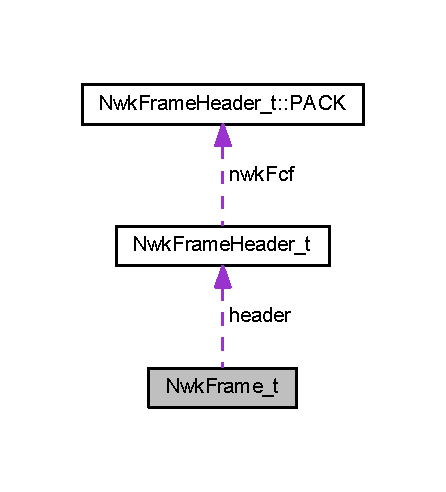
\includegraphics[width=214pt]{struct_nwk_frame__t__coll__graph}
\end{center}
\end{figure}
\subsection*{Data Fields}
\begin{DoxyCompactItemize}
\item 
uint8\-\_\-t \hyperlink{struct_nwk_frame__t_a5fbf3e581463732d26ea7b242c666109}{state}
\item 
uint8\-\_\-t \hyperlink{struct_nwk_frame__t_a42934dd5ff3a529ffb264402944f77e8}{size}
\item 
\begin{tabbing}
xx\=xx\=xx\=xx\=xx\=xx\=xx\=xx\=xx\=\kill
union \{\\
\>\hyperlink{struct_nwk_frame_header__t}{NwkFrameHeader\_t} \hyperlink{struct_nwk_frame__t_ae7615117e566f339c8893bd6f6ed642d}{header}\\
\>uint8\_t \hyperlink{struct_nwk_frame__t_a504e9f54f727b77a64c482fd9c54c30d}{data} \mbox{[}\hyperlink{nwk_frame_8h_aecb889ddcbbc535190f5a83b26aa205b}{NWK\_FRAME\_MAX\_PAYLOAD\_SIZE}\mbox{]}\\
\}; \\

\end{tabbing}\item 
uint8\-\_\-t $\ast$ \hyperlink{struct_nwk_frame__t_abe0e1d3be987a1a6fe8d6b9f19cefa67}{payload}
\item 
\begin{tabbing}
xx\=xx\=xx\=xx\=xx\=xx\=xx\=xx\=xx\=\kill
union \{\\
\>struct \{\\
\>\>uint8\_t \hyperlink{struct_nwk_frame__t_ace554a195e09279c216c3efc6895e66f}{lqi}\\
\>\>int8\_t \hyperlink{struct_nwk_frame__t_ae99f976337170b91bab3c91efee0c19e}{rssi}\\
\>\} \hyperlink{struct_nwk_frame__t_af342a861746a0f6f40285195c4959a9e}{rx}\\
\>struct \{\\
\>\>uint8\_t \hyperlink{struct_nwk_frame__t_ad6257c1abbda87dc2a653a6086f8e9e5}{status}\\
\>\>uint16\_t \hyperlink{struct_nwk_frame__t_a3c49425f94b27976baefc90d1549ffab}{timeout}\\
\>\>uint8\_t \hyperlink{struct_nwk_frame__t_a71639d3ef8b8ced3f027c8cd5b41a780}{control}\\
\>\>void($\ast$ \hyperlink{struct_nwk_frame__t_a7b39f6281e35afdcbb31cbf4f959d639}{confirm} )(struct \hyperlink{struct_nwk_frame__t}{NwkFrame\_t} $\ast$frame)\\
\>\} \hyperlink{struct_nwk_frame__t_ab5e3dc31787a24bb22a62465358d71ba}{tx}\\
\}; \\

\end{tabbing}\end{DoxyCompactItemize}


\subsection{Field Documentation}
\hypertarget{struct_nwk_frame__t_a620850c2e91356398fae4bee93a792cc}{\subsubsection[{"@3}]{\setlength{\rightskip}{0pt plus 5cm}union \{ ... \} }}\label{struct_nwk_frame__t_a620850c2e91356398fae4bee93a792cc}
\hypertarget{struct_nwk_frame__t_acffc95e38f5718cde3313373af1cf6d0}{\subsubsection[{"@5}]{\setlength{\rightskip}{0pt plus 5cm}union \{ ... \} }}\label{struct_nwk_frame__t_acffc95e38f5718cde3313373af1cf6d0}
\hypertarget{struct_nwk_frame__t_a7b39f6281e35afdcbb31cbf4f959d639}{\index{Nwk\-Frame\-\_\-t@{Nwk\-Frame\-\_\-t}!confirm@{confirm}}
\index{confirm@{confirm}!NwkFrame_t@{Nwk\-Frame\-\_\-t}}
\subsubsection[{confirm}]{\setlength{\rightskip}{0pt plus 5cm}void($\ast$ Nwk\-Frame\-\_\-t\-::confirm)(struct {\bf Nwk\-Frame\-\_\-t} $\ast$frame)}}\label{struct_nwk_frame__t_a7b39f6281e35afdcbb31cbf4f959d639}
\hypertarget{struct_nwk_frame__t_a71639d3ef8b8ced3f027c8cd5b41a780}{\index{Nwk\-Frame\-\_\-t@{Nwk\-Frame\-\_\-t}!control@{control}}
\index{control@{control}!NwkFrame_t@{Nwk\-Frame\-\_\-t}}
\subsubsection[{control}]{\setlength{\rightskip}{0pt plus 5cm}uint8\-\_\-t Nwk\-Frame\-\_\-t\-::control}}\label{struct_nwk_frame__t_a71639d3ef8b8ced3f027c8cd5b41a780}
\hypertarget{struct_nwk_frame__t_a504e9f54f727b77a64c482fd9c54c30d}{\index{Nwk\-Frame\-\_\-t@{Nwk\-Frame\-\_\-t}!data@{data}}
\index{data@{data}!NwkFrame_t@{Nwk\-Frame\-\_\-t}}
\subsubsection[{data}]{\setlength{\rightskip}{0pt plus 5cm}uint8\-\_\-t Nwk\-Frame\-\_\-t\-::data\mbox{[}{\bf N\-W\-K\-\_\-\-F\-R\-A\-M\-E\-\_\-\-M\-A\-X\-\_\-\-P\-A\-Y\-L\-O\-A\-D\-\_\-\-S\-I\-Z\-E}\mbox{]}}}\label{struct_nwk_frame__t_a504e9f54f727b77a64c482fd9c54c30d}


Referenced by nwk\-Frame\-Alloc(), nwk\-Frame\-Payload\-Size(), nwk\-Tx\-Broadcast\-Frame(), nwk\-Tx\-Task\-Handler(), and P\-H\-Y\-\_\-\-Data\-Ind().

\hypertarget{struct_nwk_frame__t_ae7615117e566f339c8893bd6f6ed642d}{\index{Nwk\-Frame\-\_\-t@{Nwk\-Frame\-\_\-t}!header@{header}}
\index{header@{header}!NwkFrame_t@{Nwk\-Frame\-\_\-t}}
\subsubsection[{header}]{\setlength{\rightskip}{0pt plus 5cm}{\bf Nwk\-Frame\-Header\-\_\-t} Nwk\-Frame\-\_\-t\-::header}}\label{struct_nwk_frame__t_ae7615117e566f339c8893bd6f6ed642d}


Referenced by nwk\-Data\-Req\-Send\-Frame(), nwk\-Frame\-Command\-Init(), nwk\-Rx\-Handle\-Indication(), nwk\-Rx\-Handle\-Received\-Frame(), nwk\-Rx\-Indicate\-Frame(), nwk\-Rx\-Send\-Ack(), nwk\-Tx\-Broadcast\-Frame(), nwk\-Tx\-Frame(), and nwk\-Tx\-Task\-Handler().

\hypertarget{struct_nwk_frame__t_ace554a195e09279c216c3efc6895e66f}{\index{Nwk\-Frame\-\_\-t@{Nwk\-Frame\-\_\-t}!lqi@{lqi}}
\index{lqi@{lqi}!NwkFrame_t@{Nwk\-Frame\-\_\-t}}
\subsubsection[{lqi}]{\setlength{\rightskip}{0pt plus 5cm}uint8\-\_\-t Nwk\-Frame\-\_\-t\-::lqi}}\label{struct_nwk_frame__t_ace554a195e09279c216c3efc6895e66f}
\hypertarget{struct_nwk_frame__t_abe0e1d3be987a1a6fe8d6b9f19cefa67}{\index{Nwk\-Frame\-\_\-t@{Nwk\-Frame\-\_\-t}!payload@{payload}}
\index{payload@{payload}!NwkFrame_t@{Nwk\-Frame\-\_\-t}}
\subsubsection[{payload}]{\setlength{\rightskip}{0pt plus 5cm}uint8\-\_\-t$\ast$ Nwk\-Frame\-\_\-t\-::payload}}\label{struct_nwk_frame__t_abe0e1d3be987a1a6fe8d6b9f19cefa67}


Referenced by nwk\-Data\-Req\-Send\-Frame(), nwk\-Frame\-Alloc(), nwk\-Frame\-Payload\-Size(), nwk\-Rx\-Handle\-Received\-Frame(), nwk\-Rx\-Indicate\-Frame(), and nwk\-Rx\-Send\-Ack().

\hypertarget{struct_nwk_frame__t_ae99f976337170b91bab3c91efee0c19e}{\index{Nwk\-Frame\-\_\-t@{Nwk\-Frame\-\_\-t}!rssi@{rssi}}
\index{rssi@{rssi}!NwkFrame_t@{Nwk\-Frame\-\_\-t}}
\subsubsection[{rssi}]{\setlength{\rightskip}{0pt plus 5cm}int8\-\_\-t Nwk\-Frame\-\_\-t\-::rssi}}\label{struct_nwk_frame__t_ae99f976337170b91bab3c91efee0c19e}
\hypertarget{struct_nwk_frame__t_af342a861746a0f6f40285195c4959a9e}{\index{Nwk\-Frame\-\_\-t@{Nwk\-Frame\-\_\-t}!rx@{rx}}
\index{rx@{rx}!NwkFrame_t@{Nwk\-Frame\-\_\-t}}
\subsubsection[{rx}]{\setlength{\rightskip}{0pt plus 5cm}struct \{ ... \}   Nwk\-Frame\-\_\-t\-::rx}}\label{struct_nwk_frame__t_af342a861746a0f6f40285195c4959a9e}


Referenced by nwk\-Rx\-Handle\-Received\-Frame(), nwk\-Rx\-Indicate\-Frame(), and P\-H\-Y\-\_\-\-Data\-Ind().

\hypertarget{struct_nwk_frame__t_a42934dd5ff3a529ffb264402944f77e8}{\index{Nwk\-Frame\-\_\-t@{Nwk\-Frame\-\_\-t}!size@{size}}
\index{size@{size}!NwkFrame_t@{Nwk\-Frame\-\_\-t}}
\subsubsection[{size}]{\setlength{\rightskip}{0pt plus 5cm}uint8\-\_\-t Nwk\-Frame\-\_\-t\-::size}}\label{struct_nwk_frame__t_a42934dd5ff3a529ffb264402944f77e8}


Referenced by nwk\-Data\-Req\-Send\-Frame(), nwk\-Frame\-Alloc(), nwk\-Frame\-Payload\-Size(), nwk\-Rx\-Send\-Ack(), nwk\-Tx\-Broadcast\-Frame(), nwk\-Tx\-Task\-Handler(), and P\-H\-Y\-\_\-\-Data\-Ind().

\hypertarget{struct_nwk_frame__t_a5fbf3e581463732d26ea7b242c666109}{\index{Nwk\-Frame\-\_\-t@{Nwk\-Frame\-\_\-t}!state@{state}}
\index{state@{state}!NwkFrame_t@{Nwk\-Frame\-\_\-t}}
\subsubsection[{state}]{\setlength{\rightskip}{0pt plus 5cm}uint8\-\_\-t Nwk\-Frame\-\_\-t\-::state}}\label{struct_nwk_frame__t_a5fbf3e581463732d26ea7b242c666109}


Referenced by nwk\-Frame\-Free(), nwk\-Frame\-Next(), nwk\-Rx\-Handle\-Indication(), nwk\-Rx\-Handle\-Received\-Frame(), nwk\-Rx\-Task\-Handler(), nwk\-Tx\-Ack\-Received(), nwk\-Tx\-Ack\-Wait\-Timer\-Handler(), nwk\-Tx\-Broadcast\-Frame(), nwk\-Tx\-Confirm(), nwk\-Tx\-Delay\-Timer\-Handler(), nwk\-Tx\-Frame(), nwk\-Tx\-Task\-Handler(), P\-H\-Y\-\_\-\-Data\-Conf(), and P\-H\-Y\-\_\-\-Data\-Ind().

\hypertarget{struct_nwk_frame__t_ad6257c1abbda87dc2a653a6086f8e9e5}{\index{Nwk\-Frame\-\_\-t@{Nwk\-Frame\-\_\-t}!status@{status}}
\index{status@{status}!NwkFrame_t@{Nwk\-Frame\-\_\-t}}
\subsubsection[{status}]{\setlength{\rightskip}{0pt plus 5cm}uint8\-\_\-t Nwk\-Frame\-\_\-t\-::status}}\label{struct_nwk_frame__t_ad6257c1abbda87dc2a653a6086f8e9e5}
\hypertarget{struct_nwk_frame__t_a3c49425f94b27976baefc90d1549ffab}{\index{Nwk\-Frame\-\_\-t@{Nwk\-Frame\-\_\-t}!timeout@{timeout}}
\index{timeout@{timeout}!NwkFrame_t@{Nwk\-Frame\-\_\-t}}
\subsubsection[{timeout}]{\setlength{\rightskip}{0pt plus 5cm}uint16\-\_\-t Nwk\-Frame\-\_\-t\-::timeout}}\label{struct_nwk_frame__t_a3c49425f94b27976baefc90d1549ffab}
\hypertarget{struct_nwk_frame__t_ab5e3dc31787a24bb22a62465358d71ba}{\index{Nwk\-Frame\-\_\-t@{Nwk\-Frame\-\_\-t}!tx@{tx}}
\index{tx@{tx}!NwkFrame_t@{Nwk\-Frame\-\_\-t}}
\subsubsection[{tx}]{\setlength{\rightskip}{0pt plus 5cm}struct \{ ... \}   Nwk\-Frame\-\_\-t\-::tx}}\label{struct_nwk_frame__t_ab5e3dc31787a24bb22a62465358d71ba}


Referenced by nwk\-Data\-Req\-Send\-Frame(), nwk\-Data\-Req\-Tx\-Conf(), nwk\-Frame\-Command\-Init(), nwk\-Rx\-Send\-Ack(), nwk\-Tx\-Ack\-Wait\-Timer\-Handler(), nwk\-Tx\-Broadcast\-Frame(), nwk\-Tx\-Confirm(), nwk\-Tx\-Delay\-Timer\-Handler(), nwk\-Tx\-Frame(), nwk\-Tx\-Task\-Handler(), and P\-H\-Y\-\_\-\-Data\-Conf().



The documentation for this struct was generated from the following file\-:\begin{DoxyCompactItemize}
\item 
C\-:/\-Users/\-A\-B/\-Documents/\-Git\-Hub/\-A\-T\-M\-E\-L-\/\-A\-T\-M\-O\-S/\-A\-T\-M\-O\-S/nwk/inc/\hyperlink{nwk_frame_8h}{nwk\-Frame.\-h}\end{DoxyCompactItemize}

\hypertarget{struct_nwk_frame_header__t}{\section{Nwk\-Frame\-Header\-\_\-t Struct Reference}
\label{struct_nwk_frame_header__t}\index{Nwk\-Frame\-Header\-\_\-t@{Nwk\-Frame\-Header\-\_\-t}}
}


{\ttfamily \#include $<$nwk\-Frame.\-h$>$}



Collaboration diagram for Nwk\-Frame\-Header\-\_\-t\-:
\nopagebreak
\begin{figure}[H]
\begin{center}
\leavevmode
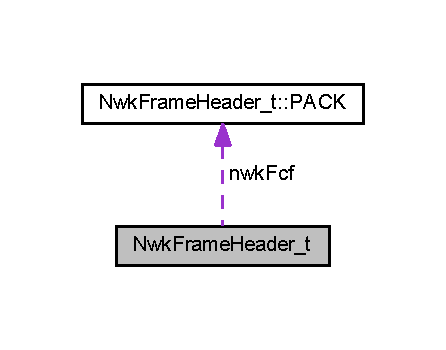
\includegraphics[width=214pt]{struct_nwk_frame_header__t__coll__graph}
\end{center}
\end{figure}
\subsection*{Data Structures}
\begin{DoxyCompactItemize}
\item 
struct \hyperlink{struct_nwk_frame_header__t_1_1_p_a_c_k}{P\-A\-C\-K}
\end{DoxyCompactItemize}
\subsection*{Data Fields}
\begin{DoxyCompactItemize}
\item 
uint16\-\_\-t \hyperlink{struct_nwk_frame_header__t_a136fb8b5fae16dc89aa581578163a292}{mac\-Fcf}
\item 
uint8\-\_\-t \hyperlink{struct_nwk_frame_header__t_a1a2af294d7235b16d1bff5050fe8c24d}{mac\-Seq}
\item 
uint16\-\_\-t \hyperlink{struct_nwk_frame_header__t_a503c00407e350a489337324ea735f421}{mac\-Dst\-Pan\-Id}
\item 
uint16\-\_\-t \hyperlink{struct_nwk_frame_header__t_a52eaa8a2d2442746a409f26742205433}{mac\-Dst\-Addr}
\item 
uint16\-\_\-t \hyperlink{struct_nwk_frame_header__t_a8648deb85dac8f29a2109e0e430b1be3}{mac\-Src\-Addr}
\item 
struct \hyperlink{sys_types_8h_a085f543ccded0731c1191e9c76a27311}{Nwk\-Frame\-Header\-\_\-t\-::\-P\-A\-C\-K} \hyperlink{struct_nwk_frame_header__t_a0db7c5ebd8f56586b41063be79f69d5a}{nwk\-Fcf}
\item 
uint8\-\_\-t \hyperlink{struct_nwk_frame_header__t_a198e5b4ebb92d3b58b38dfa6a1a836e4}{nwk\-Seq}
\item 
uint16\-\_\-t \hyperlink{struct_nwk_frame_header__t_a4e62b8b0c4a47f8fc152f3f5e05db61a}{nwk\-Src\-Addr}
\item 
uint16\-\_\-t \hyperlink{struct_nwk_frame_header__t_a73226e1cb8813883d7c5ce8e9bf7ef40}{nwk\-Dst\-Addr}
\end{DoxyCompactItemize}


\subsection{Field Documentation}
\hypertarget{struct_nwk_frame_header__t_a52eaa8a2d2442746a409f26742205433}{\index{Nwk\-Frame\-Header\-\_\-t@{Nwk\-Frame\-Header\-\_\-t}!mac\-Dst\-Addr@{mac\-Dst\-Addr}}
\index{mac\-Dst\-Addr@{mac\-Dst\-Addr}!NwkFrameHeader_t@{Nwk\-Frame\-Header\-\_\-t}}
\subsubsection[{mac\-Dst\-Addr}]{\setlength{\rightskip}{0pt plus 5cm}uint16\-\_\-t Nwk\-Frame\-Header\-\_\-t\-::mac\-Dst\-Addr}}\label{struct_nwk_frame_header__t_a52eaa8a2d2442746a409f26742205433}


Referenced by nwk\-Rx\-Handle\-Indication(), nwk\-Rx\-Handle\-Received\-Frame(), nwk\-Rx\-Reject\-Duplicate(), nwk\-Tx\-Broadcast\-Frame(), and nwk\-Tx\-Frame().

\hypertarget{struct_nwk_frame_header__t_a503c00407e350a489337324ea735f421}{\index{Nwk\-Frame\-Header\-\_\-t@{Nwk\-Frame\-Header\-\_\-t}!mac\-Dst\-Pan\-Id@{mac\-Dst\-Pan\-Id}}
\index{mac\-Dst\-Pan\-Id@{mac\-Dst\-Pan\-Id}!NwkFrameHeader_t@{Nwk\-Frame\-Header\-\_\-t}}
\subsubsection[{mac\-Dst\-Pan\-Id}]{\setlength{\rightskip}{0pt plus 5cm}uint16\-\_\-t Nwk\-Frame\-Header\-\_\-t\-::mac\-Dst\-Pan\-Id}}\label{struct_nwk_frame_header__t_a503c00407e350a489337324ea735f421}


Referenced by nwk\-Rx\-Handle\-Indication(), nwk\-Rx\-Handle\-Received\-Frame(), nwk\-Rx\-Indicate\-Frame(), nwk\-Tx\-Broadcast\-Frame(), and nwk\-Tx\-Frame().

\hypertarget{struct_nwk_frame_header__t_a136fb8b5fae16dc89aa581578163a292}{\index{Nwk\-Frame\-Header\-\_\-t@{Nwk\-Frame\-Header\-\_\-t}!mac\-Fcf@{mac\-Fcf}}
\index{mac\-Fcf@{mac\-Fcf}!NwkFrameHeader_t@{Nwk\-Frame\-Header\-\_\-t}}
\subsubsection[{mac\-Fcf}]{\setlength{\rightskip}{0pt plus 5cm}uint16\-\_\-t Nwk\-Frame\-Header\-\_\-t\-::mac\-Fcf}}\label{struct_nwk_frame_header__t_a136fb8b5fae16dc89aa581578163a292}


Referenced by nwk\-Tx\-Broadcast\-Frame(), and nwk\-Tx\-Frame().

\hypertarget{struct_nwk_frame_header__t_a1a2af294d7235b16d1bff5050fe8c24d}{\index{Nwk\-Frame\-Header\-\_\-t@{Nwk\-Frame\-Header\-\_\-t}!mac\-Seq@{mac\-Seq}}
\index{mac\-Seq@{mac\-Seq}!NwkFrameHeader_t@{Nwk\-Frame\-Header\-\_\-t}}
\subsubsection[{mac\-Seq}]{\setlength{\rightskip}{0pt plus 5cm}uint8\-\_\-t Nwk\-Frame\-Header\-\_\-t\-::mac\-Seq}}\label{struct_nwk_frame_header__t_a1a2af294d7235b16d1bff5050fe8c24d}


Referenced by nwk\-Tx\-Broadcast\-Frame(), and nwk\-Tx\-Frame().

\hypertarget{struct_nwk_frame_header__t_a8648deb85dac8f29a2109e0e430b1be3}{\index{Nwk\-Frame\-Header\-\_\-t@{Nwk\-Frame\-Header\-\_\-t}!mac\-Src\-Addr@{mac\-Src\-Addr}}
\index{mac\-Src\-Addr@{mac\-Src\-Addr}!NwkFrameHeader_t@{Nwk\-Frame\-Header\-\_\-t}}
\subsubsection[{mac\-Src\-Addr}]{\setlength{\rightskip}{0pt plus 5cm}uint16\-\_\-t Nwk\-Frame\-Header\-\_\-t\-::mac\-Src\-Addr}}\label{struct_nwk_frame_header__t_a8648deb85dac8f29a2109e0e430b1be3}


Referenced by nwk\-Rx\-Handle\-Received\-Frame(), nwk\-Rx\-Indicate\-Frame(), nwk\-Tx\-Broadcast\-Frame(), and nwk\-Tx\-Frame().

\hypertarget{struct_nwk_frame_header__t_a73226e1cb8813883d7c5ce8e9bf7ef40}{\index{Nwk\-Frame\-Header\-\_\-t@{Nwk\-Frame\-Header\-\_\-t}!nwk\-Dst\-Addr@{nwk\-Dst\-Addr}}
\index{nwk\-Dst\-Addr@{nwk\-Dst\-Addr}!NwkFrameHeader_t@{Nwk\-Frame\-Header\-\_\-t}}
\subsubsection[{nwk\-Dst\-Addr}]{\setlength{\rightskip}{0pt plus 5cm}uint16\-\_\-t Nwk\-Frame\-Header\-\_\-t\-::nwk\-Dst\-Addr}}\label{struct_nwk_frame_header__t_a73226e1cb8813883d7c5ce8e9bf7ef40}


Referenced by nwk\-Data\-Req\-Send\-Frame(), nwk\-Rx\-Handle\-Indication(), nwk\-Rx\-Handle\-Received\-Frame(), nwk\-Rx\-Indicate\-Frame(), nwk\-Rx\-Reject\-Duplicate(), nwk\-Rx\-Send\-Ack(), and nwk\-Tx\-Frame().

\hypertarget{struct_nwk_frame_header__t_a0db7c5ebd8f56586b41063be79f69d5a}{\index{Nwk\-Frame\-Header\-\_\-t@{Nwk\-Frame\-Header\-\_\-t}!nwk\-Fcf@{nwk\-Fcf}}
\index{nwk\-Fcf@{nwk\-Fcf}!NwkFrameHeader_t@{Nwk\-Frame\-Header\-\_\-t}}
\subsubsection[{nwk\-Fcf}]{\setlength{\rightskip}{0pt plus 5cm}struct {\bf Nwk\-Frame\-Header\-\_\-t\-::\-P\-A\-C\-K}            Nwk\-Frame\-Header\-\_\-t\-::nwk\-Fcf}}\label{struct_nwk_frame_header__t_a0db7c5ebd8f56586b41063be79f69d5a}


Referenced by nwk\-Data\-Req\-Send\-Frame(), nwk\-Frame\-Command\-Init(), nwk\-Rx\-Handle\-Indication(), nwk\-Rx\-Handle\-Received\-Frame(), nwk\-Rx\-Indicate\-Frame(), nwk\-Rx\-Reject\-Duplicate(), nwk\-Rx\-Send\-Ack(), nwk\-Tx\-Frame(), and nwk\-Tx\-Task\-Handler().

\hypertarget{struct_nwk_frame_header__t_a198e5b4ebb92d3b58b38dfa6a1a836e4}{\index{Nwk\-Frame\-Header\-\_\-t@{Nwk\-Frame\-Header\-\_\-t}!nwk\-Seq@{nwk\-Seq}}
\index{nwk\-Seq@{nwk\-Seq}!NwkFrameHeader_t@{Nwk\-Frame\-Header\-\_\-t}}
\subsubsection[{nwk\-Seq}]{\setlength{\rightskip}{0pt plus 5cm}uint8\-\_\-t Nwk\-Frame\-Header\-\_\-t\-::nwk\-Seq}}\label{struct_nwk_frame_header__t_a198e5b4ebb92d3b58b38dfa6a1a836e4}


Referenced by nwk\-Data\-Req\-Send\-Frame(), nwk\-Frame\-Command\-Init(), nwk\-Rx\-Reject\-Duplicate(), and nwk\-Rx\-Send\-Ack().

\hypertarget{struct_nwk_frame_header__t_a4e62b8b0c4a47f8fc152f3f5e05db61a}{\index{Nwk\-Frame\-Header\-\_\-t@{Nwk\-Frame\-Header\-\_\-t}!nwk\-Src\-Addr@{nwk\-Src\-Addr}}
\index{nwk\-Src\-Addr@{nwk\-Src\-Addr}!NwkFrameHeader_t@{Nwk\-Frame\-Header\-\_\-t}}
\subsubsection[{nwk\-Src\-Addr}]{\setlength{\rightskip}{0pt plus 5cm}uint16\-\_\-t Nwk\-Frame\-Header\-\_\-t\-::nwk\-Src\-Addr}}\label{struct_nwk_frame_header__t_a4e62b8b0c4a47f8fc152f3f5e05db61a}


Referenced by nwk\-Data\-Req\-Send\-Frame(), nwk\-Frame\-Command\-Init(), nwk\-Rx\-Handle\-Received\-Frame(), nwk\-Rx\-Indicate\-Frame(), nwk\-Rx\-Reject\-Duplicate(), nwk\-Rx\-Send\-Ack(), and nwk\-Tx\-Task\-Handler().



The documentation for this struct was generated from the following file\-:\begin{DoxyCompactItemize}
\item 
C\-:/\-Users/\-A\-B/\-Documents/\-Git\-Hub/\-A\-T\-M\-E\-L-\/\-A\-T\-M\-O\-S/\-A\-T\-M\-O\-S/nwk/inc/\hyperlink{nwk_frame_8h}{nwk\-Frame.\-h}\end{DoxyCompactItemize}

\hypertarget{struct_nwk_frame_multicast_header__t}{\section{Nwk\-Frame\-Multicast\-Header\-\_\-t Struct Reference}
\label{struct_nwk_frame_multicast_header__t}\index{Nwk\-Frame\-Multicast\-Header\-\_\-t@{Nwk\-Frame\-Multicast\-Header\-\_\-t}}
}


{\ttfamily \#include $<$nwk\-Frame.\-h$>$}

\subsection*{Data Fields}
\begin{DoxyCompactItemize}
\item 
uint16\-\_\-t \hyperlink{struct_nwk_frame_multicast_header__t_ae345f9729f9f70acb56384c58b74d7fe}{non\-Member\-Radius}\-: 4
\item 
uint16\-\_\-t \hyperlink{struct_nwk_frame_multicast_header__t_ad93a788fcf5ef8690deb6681406ddde7}{max\-Non\-Member\-Radius}\-: 4
\item 
uint16\-\_\-t \hyperlink{struct_nwk_frame_multicast_header__t_abfc3e12c48cebacbe72f2db5f812fd71}{member\-Radius}\-: 4
\item 
uint16\-\_\-t \hyperlink{struct_nwk_frame_multicast_header__t_acc3e739b6ab868df1fb4e4d0ee20fa77}{max\-Member\-Radius}\-: 4
\end{DoxyCompactItemize}


\subsection{Field Documentation}
\hypertarget{struct_nwk_frame_multicast_header__t_acc3e739b6ab868df1fb4e4d0ee20fa77}{\index{Nwk\-Frame\-Multicast\-Header\-\_\-t@{Nwk\-Frame\-Multicast\-Header\-\_\-t}!max\-Member\-Radius@{max\-Member\-Radius}}
\index{max\-Member\-Radius@{max\-Member\-Radius}!NwkFrameMulticastHeader_t@{Nwk\-Frame\-Multicast\-Header\-\_\-t}}
\subsubsection[{max\-Member\-Radius}]{\setlength{\rightskip}{0pt plus 5cm}uint16\-\_\-t Nwk\-Frame\-Multicast\-Header\-\_\-t\-::max\-Member\-Radius}}\label{struct_nwk_frame_multicast_header__t_acc3e739b6ab868df1fb4e4d0ee20fa77}


Referenced by nwk\-Data\-Req\-Send\-Frame(), and nwk\-Rx\-Handle\-Received\-Frame().

\hypertarget{struct_nwk_frame_multicast_header__t_ad93a788fcf5ef8690deb6681406ddde7}{\index{Nwk\-Frame\-Multicast\-Header\-\_\-t@{Nwk\-Frame\-Multicast\-Header\-\_\-t}!max\-Non\-Member\-Radius@{max\-Non\-Member\-Radius}}
\index{max\-Non\-Member\-Radius@{max\-Non\-Member\-Radius}!NwkFrameMulticastHeader_t@{Nwk\-Frame\-Multicast\-Header\-\_\-t}}
\subsubsection[{max\-Non\-Member\-Radius}]{\setlength{\rightskip}{0pt plus 5cm}uint16\-\_\-t Nwk\-Frame\-Multicast\-Header\-\_\-t\-::max\-Non\-Member\-Radius}}\label{struct_nwk_frame_multicast_header__t_ad93a788fcf5ef8690deb6681406ddde7}


Referenced by nwk\-Data\-Req\-Send\-Frame(), and nwk\-Rx\-Handle\-Received\-Frame().

\hypertarget{struct_nwk_frame_multicast_header__t_abfc3e12c48cebacbe72f2db5f812fd71}{\index{Nwk\-Frame\-Multicast\-Header\-\_\-t@{Nwk\-Frame\-Multicast\-Header\-\_\-t}!member\-Radius@{member\-Radius}}
\index{member\-Radius@{member\-Radius}!NwkFrameMulticastHeader_t@{Nwk\-Frame\-Multicast\-Header\-\_\-t}}
\subsubsection[{member\-Radius}]{\setlength{\rightskip}{0pt plus 5cm}uint16\-\_\-t Nwk\-Frame\-Multicast\-Header\-\_\-t\-::member\-Radius}}\label{struct_nwk_frame_multicast_header__t_abfc3e12c48cebacbe72f2db5f812fd71}


Referenced by nwk\-Data\-Req\-Send\-Frame(), and nwk\-Rx\-Handle\-Received\-Frame().

\hypertarget{struct_nwk_frame_multicast_header__t_ae345f9729f9f70acb56384c58b74d7fe}{\index{Nwk\-Frame\-Multicast\-Header\-\_\-t@{Nwk\-Frame\-Multicast\-Header\-\_\-t}!non\-Member\-Radius@{non\-Member\-Radius}}
\index{non\-Member\-Radius@{non\-Member\-Radius}!NwkFrameMulticastHeader_t@{Nwk\-Frame\-Multicast\-Header\-\_\-t}}
\subsubsection[{non\-Member\-Radius}]{\setlength{\rightskip}{0pt plus 5cm}uint16\-\_\-t Nwk\-Frame\-Multicast\-Header\-\_\-t\-::non\-Member\-Radius}}\label{struct_nwk_frame_multicast_header__t_ae345f9729f9f70acb56384c58b74d7fe}


Referenced by nwk\-Data\-Req\-Send\-Frame(), and nwk\-Rx\-Handle\-Received\-Frame().



The documentation for this struct was generated from the following file\-:\begin{DoxyCompactItemize}
\item 
C\-:/\-Users/\-A\-B/\-Documents/\-Git\-Hub/\-A\-T\-M\-E\-L-\/\-A\-T\-M\-O\-S/\-A\-T\-M\-O\-S/nwk/inc/\hyperlink{nwk_frame_8h}{nwk\-Frame.\-h}\end{DoxyCompactItemize}

\hypertarget{struct_nwk_ib__t}{\section{Nwk\-Ib\-\_\-t Struct Reference}
\label{struct_nwk_ib__t}\index{Nwk\-Ib\-\_\-t@{Nwk\-Ib\-\_\-t}}
}


{\ttfamily \#include $<$nwk.\-h$>$}

\subsection*{Data Fields}
\begin{DoxyCompactItemize}
\item 
uint16\-\_\-t \hyperlink{struct_nwk_ib__t_a93d41c50b1fc0979fdcb5b31525b64a3}{addr}
\item 
uint16\-\_\-t \hyperlink{struct_nwk_ib__t_a421fbf7eaa40857b90ed458d8648e774}{pan\-Id}
\item 
uint8\-\_\-t \hyperlink{struct_nwk_ib__t_a7922253056ebd63dd2c8fce7164e71d6}{nwk\-Seq\-Num}
\item 
uint8\-\_\-t \hyperlink{struct_nwk_ib__t_a17330655f00d16fb7a4732d55c8ce646}{mac\-Seq\-Num}
\item 
bool($\ast$ \hyperlink{struct_nwk_ib__t_a6884c7984dc4010d48772d84fd9b83bc}{endpoint} \mbox{[}\hyperlink{nwk_8h_aeed58979d2ea2db91c59f556223da4ae}{N\-W\-K\-\_\-\-E\-N\-D\-P\-O\-I\-N\-T\-S\-\_\-\-A\-M\-O\-U\-N\-T}\mbox{]})(\hyperlink{struct_n_w_k___data_ind__t}{N\-W\-K\-\_\-\-Data\-Ind\-\_\-t} $\ast$ind)
\item 
uint16\-\_\-t \hyperlink{struct_nwk_ib__t_a577806f9b0e40c84e2c8235b3479f759}{lock}
\end{DoxyCompactItemize}


\subsection{Field Documentation}
\hypertarget{struct_nwk_ib__t_a93d41c50b1fc0979fdcb5b31525b64a3}{\index{Nwk\-Ib\-\_\-t@{Nwk\-Ib\-\_\-t}!addr@{addr}}
\index{addr@{addr}!NwkIb_t@{Nwk\-Ib\-\_\-t}}
\subsubsection[{addr}]{\setlength{\rightskip}{0pt plus 5cm}uint16\-\_\-t Nwk\-Ib\-\_\-t\-::addr}}\label{struct_nwk_ib__t_a93d41c50b1fc0979fdcb5b31525b64a3}


Referenced by N\-W\-K\-\_\-\-Init(), N\-W\-K\-\_\-\-Set\-Addr(), nwk\-Data\-Req\-Send\-Frame(), nwk\-Frame\-Command\-Init(), nwk\-Rx\-Handle\-Indication(), nwk\-Rx\-Handle\-Received\-Frame(), nwk\-Rx\-Reject\-Duplicate(), nwk\-Tx\-Broadcast\-Frame(), nwk\-Tx\-Frame(), and nwk\-Tx\-Task\-Handler().

\hypertarget{struct_nwk_ib__t_a6884c7984dc4010d48772d84fd9b83bc}{\index{Nwk\-Ib\-\_\-t@{Nwk\-Ib\-\_\-t}!endpoint@{endpoint}}
\index{endpoint@{endpoint}!NwkIb_t@{Nwk\-Ib\-\_\-t}}
\subsubsection[{endpoint}]{\setlength{\rightskip}{0pt plus 5cm}bool($\ast$ Nwk\-Ib\-\_\-t\-::endpoint\mbox{[}{\bf N\-W\-K\-\_\-\-E\-N\-D\-P\-O\-I\-N\-T\-S\-\_\-\-A\-M\-O\-U\-N\-T}\mbox{]})({\bf N\-W\-K\-\_\-\-Data\-Ind\-\_\-t} $\ast$ind)}}\label{struct_nwk_ib__t_a6884c7984dc4010d48772d84fd9b83bc}


Referenced by N\-W\-K\-\_\-\-Init(), N\-W\-K\-\_\-\-Open\-Endpoint(), and nwk\-Rx\-Indicate\-Frame().

\hypertarget{struct_nwk_ib__t_a577806f9b0e40c84e2c8235b3479f759}{\index{Nwk\-Ib\-\_\-t@{Nwk\-Ib\-\_\-t}!lock@{lock}}
\index{lock@{lock}!NwkIb_t@{Nwk\-Ib\-\_\-t}}
\subsubsection[{lock}]{\setlength{\rightskip}{0pt plus 5cm}uint16\-\_\-t Nwk\-Ib\-\_\-t\-::lock}}\label{struct_nwk_ib__t_a577806f9b0e40c84e2c8235b3479f759}


Referenced by N\-W\-K\-\_\-\-Busy(), N\-W\-K\-\_\-\-Data\-Req(), N\-W\-K\-\_\-\-Init(), N\-W\-K\-\_\-\-Lock(), N\-W\-K\-\_\-\-Unlock(), nwk\-Data\-Req\-Confirm(), nwk\-Frame\-Alloc(), nwk\-Frame\-Free(), nwk\-Tx\-Task\-Handler(), and P\-H\-Y\-\_\-\-Data\-Conf().

\hypertarget{struct_nwk_ib__t_a17330655f00d16fb7a4732d55c8ce646}{\index{Nwk\-Ib\-\_\-t@{Nwk\-Ib\-\_\-t}!mac\-Seq\-Num@{mac\-Seq\-Num}}
\index{mac\-Seq\-Num@{mac\-Seq\-Num}!NwkIb_t@{Nwk\-Ib\-\_\-t}}
\subsubsection[{mac\-Seq\-Num}]{\setlength{\rightskip}{0pt plus 5cm}uint8\-\_\-t Nwk\-Ib\-\_\-t\-::mac\-Seq\-Num}}\label{struct_nwk_ib__t_a17330655f00d16fb7a4732d55c8ce646}


Referenced by N\-W\-K\-\_\-\-Init(), nwk\-Tx\-Broadcast\-Frame(), and nwk\-Tx\-Frame().

\hypertarget{struct_nwk_ib__t_a7922253056ebd63dd2c8fce7164e71d6}{\index{Nwk\-Ib\-\_\-t@{Nwk\-Ib\-\_\-t}!nwk\-Seq\-Num@{nwk\-Seq\-Num}}
\index{nwk\-Seq\-Num@{nwk\-Seq\-Num}!NwkIb_t@{Nwk\-Ib\-\_\-t}}
\subsubsection[{nwk\-Seq\-Num}]{\setlength{\rightskip}{0pt plus 5cm}uint8\-\_\-t Nwk\-Ib\-\_\-t\-::nwk\-Seq\-Num}}\label{struct_nwk_ib__t_a7922253056ebd63dd2c8fce7164e71d6}


Referenced by N\-W\-K\-\_\-\-Init(), nwk\-Data\-Req\-Send\-Frame(), and nwk\-Frame\-Command\-Init().

\hypertarget{struct_nwk_ib__t_a421fbf7eaa40857b90ed458d8648e774}{\index{Nwk\-Ib\-\_\-t@{Nwk\-Ib\-\_\-t}!pan\-Id@{pan\-Id}}
\index{pan\-Id@{pan\-Id}!NwkIb_t@{Nwk\-Ib\-\_\-t}}
\subsubsection[{pan\-Id}]{\setlength{\rightskip}{0pt plus 5cm}uint16\-\_\-t Nwk\-Ib\-\_\-t\-::pan\-Id}}\label{struct_nwk_ib__t_a421fbf7eaa40857b90ed458d8648e774}


Referenced by N\-W\-K\-\_\-\-Set\-Pan\-Id(), and nwk\-Tx\-Frame().



The documentation for this struct was generated from the following file\-:\begin{DoxyCompactItemize}
\item 
C\-:/\-Users/\-A\-B/\-Documents/\-Git\-Hub/\-A\-T\-M\-E\-L-\/\-A\-T\-M\-O\-S/\-A\-T\-M\-O\-S/nwk/inc/\hyperlink{nwk_8h}{nwk.\-h}\end{DoxyCompactItemize}

\hypertarget{struct_nwk_frame_header__t_1_1_p_a_c_k}{\section{Nwk\-Frame\-Header\-\_\-t\-:\-:P\-A\-C\-K Struct Reference}
\label{struct_nwk_frame_header__t_1_1_p_a_c_k}\index{Nwk\-Frame\-Header\-\_\-t\-::\-P\-A\-C\-K@{Nwk\-Frame\-Header\-\_\-t\-::\-P\-A\-C\-K}}
}


{\ttfamily \#include $<$nwk\-Frame.\-h$>$}

\subsection*{Data Fields}
\begin{DoxyCompactItemize}
\item 
uint8\-\_\-t \hyperlink{struct_nwk_frame_header__t_1_1_p_a_c_k_a73ee22a0685511a45427ceafa7ed673e}{ack\-Request}\-: 1
\item 
uint8\-\_\-t \hyperlink{struct_nwk_frame_header__t_1_1_p_a_c_k_a0aa61ebeebfc3250134ff22b50ce8e0c}{security}\-: 1
\item 
uint8\-\_\-t \hyperlink{struct_nwk_frame_header__t_1_1_p_a_c_k_a541d170684ded70d57ef8bc691d0765a}{link\-Local}\-: 1
\item 
uint8\-\_\-t \hyperlink{struct_nwk_frame_header__t_1_1_p_a_c_k_a0e30ea53f986ac565c7e599c50e9dca2}{multicast}\-: 1
\item 
uint8\-\_\-t \hyperlink{struct_nwk_frame_header__t_1_1_p_a_c_k_aba208be46817d5bbc1bd29b970937249}{reserved}\-: 4
\item 
uint8\-\_\-t \hyperlink{struct_nwk_frame_header__t_1_1_p_a_c_k_a5aef4ba0418253c9cd3873808dac10a1}{nwk\-Src\-Endpoint}\-: 4
\item 
uint8\-\_\-t \hyperlink{struct_nwk_frame_header__t_1_1_p_a_c_k_a6ada9cf446f446dc9180b44b2dabdf98}{nwk\-Dst\-Endpoint}\-: 4
\end{DoxyCompactItemize}


\subsection{Field Documentation}
\hypertarget{struct_nwk_frame_header__t_1_1_p_a_c_k_a73ee22a0685511a45427ceafa7ed673e}{\index{Nwk\-Frame\-Header\-\_\-t\-::\-P\-A\-C\-K@{Nwk\-Frame\-Header\-\_\-t\-::\-P\-A\-C\-K}!ack\-Request@{ack\-Request}}
\index{ack\-Request@{ack\-Request}!NwkFrameHeader_t::PACK@{Nwk\-Frame\-Header\-\_\-t\-::\-P\-A\-C\-K}}
\subsubsection[{ack\-Request}]{\setlength{\rightskip}{0pt plus 5cm}uint8\-\_\-t Nwk\-Frame\-Header\-\_\-t\-::\-P\-A\-C\-K\-::ack\-Request}}\label{struct_nwk_frame_header__t_1_1_p_a_c_k_a73ee22a0685511a45427ceafa7ed673e}
\hypertarget{struct_nwk_frame_header__t_1_1_p_a_c_k_a541d170684ded70d57ef8bc691d0765a}{\index{Nwk\-Frame\-Header\-\_\-t\-::\-P\-A\-C\-K@{Nwk\-Frame\-Header\-\_\-t\-::\-P\-A\-C\-K}!link\-Local@{link\-Local}}
\index{link\-Local@{link\-Local}!NwkFrameHeader_t::PACK@{Nwk\-Frame\-Header\-\_\-t\-::\-P\-A\-C\-K}}
\subsubsection[{link\-Local}]{\setlength{\rightskip}{0pt plus 5cm}uint8\-\_\-t Nwk\-Frame\-Header\-\_\-t\-::\-P\-A\-C\-K\-::link\-Local}}\label{struct_nwk_frame_header__t_1_1_p_a_c_k_a541d170684ded70d57ef8bc691d0765a}
\hypertarget{struct_nwk_frame_header__t_1_1_p_a_c_k_a0e30ea53f986ac565c7e599c50e9dca2}{\index{Nwk\-Frame\-Header\-\_\-t\-::\-P\-A\-C\-K@{Nwk\-Frame\-Header\-\_\-t\-::\-P\-A\-C\-K}!multicast@{multicast}}
\index{multicast@{multicast}!NwkFrameHeader_t::PACK@{Nwk\-Frame\-Header\-\_\-t\-::\-P\-A\-C\-K}}
\subsubsection[{multicast}]{\setlength{\rightskip}{0pt plus 5cm}uint8\-\_\-t Nwk\-Frame\-Header\-\_\-t\-::\-P\-A\-C\-K\-::multicast}}\label{struct_nwk_frame_header__t_1_1_p_a_c_k_a0e30ea53f986ac565c7e599c50e9dca2}
\hypertarget{struct_nwk_frame_header__t_1_1_p_a_c_k_a6ada9cf446f446dc9180b44b2dabdf98}{\index{Nwk\-Frame\-Header\-\_\-t\-::\-P\-A\-C\-K@{Nwk\-Frame\-Header\-\_\-t\-::\-P\-A\-C\-K}!nwk\-Dst\-Endpoint@{nwk\-Dst\-Endpoint}}
\index{nwk\-Dst\-Endpoint@{nwk\-Dst\-Endpoint}!NwkFrameHeader_t::PACK@{Nwk\-Frame\-Header\-\_\-t\-::\-P\-A\-C\-K}}
\subsubsection[{nwk\-Dst\-Endpoint}]{\setlength{\rightskip}{0pt plus 5cm}uint8\-\_\-t Nwk\-Frame\-Header\-\_\-t\-::\-P\-A\-C\-K\-::nwk\-Dst\-Endpoint}}\label{struct_nwk_frame_header__t_1_1_p_a_c_k_a6ada9cf446f446dc9180b44b2dabdf98}
\hypertarget{struct_nwk_frame_header__t_1_1_p_a_c_k_a5aef4ba0418253c9cd3873808dac10a1}{\index{Nwk\-Frame\-Header\-\_\-t\-::\-P\-A\-C\-K@{Nwk\-Frame\-Header\-\_\-t\-::\-P\-A\-C\-K}!nwk\-Src\-Endpoint@{nwk\-Src\-Endpoint}}
\index{nwk\-Src\-Endpoint@{nwk\-Src\-Endpoint}!NwkFrameHeader_t::PACK@{Nwk\-Frame\-Header\-\_\-t\-::\-P\-A\-C\-K}}
\subsubsection[{nwk\-Src\-Endpoint}]{\setlength{\rightskip}{0pt plus 5cm}uint8\-\_\-t Nwk\-Frame\-Header\-\_\-t\-::\-P\-A\-C\-K\-::nwk\-Src\-Endpoint}}\label{struct_nwk_frame_header__t_1_1_p_a_c_k_a5aef4ba0418253c9cd3873808dac10a1}
\hypertarget{struct_nwk_frame_header__t_1_1_p_a_c_k_aba208be46817d5bbc1bd29b970937249}{\index{Nwk\-Frame\-Header\-\_\-t\-::\-P\-A\-C\-K@{Nwk\-Frame\-Header\-\_\-t\-::\-P\-A\-C\-K}!reserved@{reserved}}
\index{reserved@{reserved}!NwkFrameHeader_t::PACK@{Nwk\-Frame\-Header\-\_\-t\-::\-P\-A\-C\-K}}
\subsubsection[{reserved}]{\setlength{\rightskip}{0pt plus 5cm}uint8\-\_\-t Nwk\-Frame\-Header\-\_\-t\-::\-P\-A\-C\-K\-::reserved}}\label{struct_nwk_frame_header__t_1_1_p_a_c_k_aba208be46817d5bbc1bd29b970937249}
\hypertarget{struct_nwk_frame_header__t_1_1_p_a_c_k_a0aa61ebeebfc3250134ff22b50ce8e0c}{\index{Nwk\-Frame\-Header\-\_\-t\-::\-P\-A\-C\-K@{Nwk\-Frame\-Header\-\_\-t\-::\-P\-A\-C\-K}!security@{security}}
\index{security@{security}!NwkFrameHeader_t::PACK@{Nwk\-Frame\-Header\-\_\-t\-::\-P\-A\-C\-K}}
\subsubsection[{security}]{\setlength{\rightskip}{0pt plus 5cm}uint8\-\_\-t Nwk\-Frame\-Header\-\_\-t\-::\-P\-A\-C\-K\-::security}}\label{struct_nwk_frame_header__t_1_1_p_a_c_k_a0aa61ebeebfc3250134ff22b50ce8e0c}


The documentation for this struct was generated from the following file\-:\begin{DoxyCompactItemize}
\item 
C\-:/\-Users/\-A\-B/\-Documents/\-Git\-Hub/\-A\-T\-M\-E\-L-\/\-A\-T\-M\-O\-S/\-A\-T\-M\-O\-S/nwk/inc/\hyperlink{nwk_frame_8h}{nwk\-Frame.\-h}\end{DoxyCompactItemize}

\hypertarget{struct_p_h_y___data_ind__t}{\section{P\-H\-Y\-\_\-\-Data\-Ind\-\_\-t Struct Reference}
\label{struct_p_h_y___data_ind__t}\index{P\-H\-Y\-\_\-\-Data\-Ind\-\_\-t@{P\-H\-Y\-\_\-\-Data\-Ind\-\_\-t}}
}


{\ttfamily \#include $<$phy.\-h$>$}

\subsection*{Data Fields}
\begin{DoxyCompactItemize}
\item 
uint8\-\_\-t $\ast$ \hyperlink{struct_p_h_y___data_ind__t_abc4a667b973e3ab1841ce52c142a79b6}{data}
\item 
uint8\-\_\-t \hyperlink{struct_p_h_y___data_ind__t_ae250a8fcfc37e4af4171a8753374a53b}{size}
\item 
uint8\-\_\-t \hyperlink{struct_p_h_y___data_ind__t_a89f75514d8c2b2fdcb97a8d313636f76}{lqi}
\item 
int8\-\_\-t \hyperlink{struct_p_h_y___data_ind__t_ae39080c0fe21e6c1716222c6231d370b}{rssi}
\end{DoxyCompactItemize}


\subsection{Field Documentation}
\hypertarget{struct_p_h_y___data_ind__t_abc4a667b973e3ab1841ce52c142a79b6}{\index{P\-H\-Y\-\_\-\-Data\-Ind\-\_\-t@{P\-H\-Y\-\_\-\-Data\-Ind\-\_\-t}!data@{data}}
\index{data@{data}!PHY_DataInd_t@{P\-H\-Y\-\_\-\-Data\-Ind\-\_\-t}}
\subsubsection[{data}]{\setlength{\rightskip}{0pt plus 5cm}uint8\-\_\-t$\ast$ P\-H\-Y\-\_\-\-Data\-Ind\-\_\-t\-::data}}\label{struct_p_h_y___data_ind__t_abc4a667b973e3ab1841ce52c142a79b6}


Referenced by P\-H\-Y\-\_\-\-Data\-Ind().

\hypertarget{struct_p_h_y___data_ind__t_a89f75514d8c2b2fdcb97a8d313636f76}{\index{P\-H\-Y\-\_\-\-Data\-Ind\-\_\-t@{P\-H\-Y\-\_\-\-Data\-Ind\-\_\-t}!lqi@{lqi}}
\index{lqi@{lqi}!PHY_DataInd_t@{P\-H\-Y\-\_\-\-Data\-Ind\-\_\-t}}
\subsubsection[{lqi}]{\setlength{\rightskip}{0pt plus 5cm}uint8\-\_\-t P\-H\-Y\-\_\-\-Data\-Ind\-\_\-t\-::lqi}}\label{struct_p_h_y___data_ind__t_a89f75514d8c2b2fdcb97a8d313636f76}


Referenced by P\-H\-Y\-\_\-\-Data\-Ind().

\hypertarget{struct_p_h_y___data_ind__t_ae39080c0fe21e6c1716222c6231d370b}{\index{P\-H\-Y\-\_\-\-Data\-Ind\-\_\-t@{P\-H\-Y\-\_\-\-Data\-Ind\-\_\-t}!rssi@{rssi}}
\index{rssi@{rssi}!PHY_DataInd_t@{P\-H\-Y\-\_\-\-Data\-Ind\-\_\-t}}
\subsubsection[{rssi}]{\setlength{\rightskip}{0pt plus 5cm}int8\-\_\-t P\-H\-Y\-\_\-\-Data\-Ind\-\_\-t\-::rssi}}\label{struct_p_h_y___data_ind__t_ae39080c0fe21e6c1716222c6231d370b}


Referenced by P\-H\-Y\-\_\-\-Data\-Ind().

\hypertarget{struct_p_h_y___data_ind__t_ae250a8fcfc37e4af4171a8753374a53b}{\index{P\-H\-Y\-\_\-\-Data\-Ind\-\_\-t@{P\-H\-Y\-\_\-\-Data\-Ind\-\_\-t}!size@{size}}
\index{size@{size}!PHY_DataInd_t@{P\-H\-Y\-\_\-\-Data\-Ind\-\_\-t}}
\subsubsection[{size}]{\setlength{\rightskip}{0pt plus 5cm}uint8\-\_\-t P\-H\-Y\-\_\-\-Data\-Ind\-\_\-t\-::size}}\label{struct_p_h_y___data_ind__t_ae250a8fcfc37e4af4171a8753374a53b}


Referenced by P\-H\-Y\-\_\-\-Data\-Ind().



The documentation for this struct was generated from the following file\-:\begin{DoxyCompactItemize}
\item 
C\-:/\-Users/\-A\-B/\-Documents/\-Git\-Hub/\-A\-T\-M\-E\-L-\/\-A\-T\-M\-O\-S/\-A\-T\-M\-O\-S/phy/atmegarfr2/inc/\hyperlink{phy_8h}{phy.\-h}\end{DoxyCompactItemize}

\hypertarget{struct_s_y_s___timer__t}{\section{S\-Y\-S\-\_\-\-Timer\-\_\-t Struct Reference}
\label{struct_s_y_s___timer__t}\index{S\-Y\-S\-\_\-\-Timer\-\_\-t@{S\-Y\-S\-\_\-\-Timer\-\_\-t}}
}


{\ttfamily \#include $<$sys\-Timer.\-h$>$}



Collaboration diagram for S\-Y\-S\-\_\-\-Timer\-\_\-t\-:
\nopagebreak
\begin{figure}[H]
\begin{center}
\leavevmode
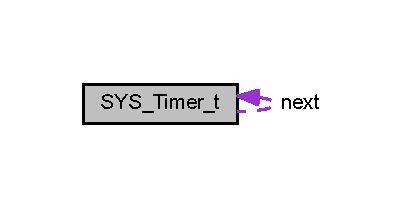
\includegraphics[width=194pt]{struct_s_y_s___timer__t__coll__graph}
\end{center}
\end{figure}
\subsection*{Data Fields}
\begin{DoxyCompactItemize}
\item 
struct \hyperlink{struct_s_y_s___timer__t}{S\-Y\-S\-\_\-\-Timer\-\_\-t} $\ast$ \hyperlink{struct_s_y_s___timer__t_af0da9cf144fe36ac5e1da4a528121820}{next}
\item 
\hyperlink{common_8h_a0ddb3f43e52282b59ee55d059ed74a28}{uint32\-\_\-t} \hyperlink{struct_s_y_s___timer__t_adf83122a4740de04c1029b1e0950ce94}{timeout}
\item 
\hyperlink{common_8h_a0ddb3f43e52282b59ee55d059ed74a28}{uint32\-\_\-t} \hyperlink{struct_s_y_s___timer__t_ac24aa7287900cd8b87e9f45bccd0b6ae}{interval}
\item 
\hyperlink{sys_timer_8h_ad3a3addd2cef39ce7fc9698efeb59cd5}{S\-Y\-S\-\_\-\-Timer\-Mode\-\_\-t} \hyperlink{struct_s_y_s___timer__t_ab992b241678bdcf98275a5de6ad81c5d}{mode}
\item 
void($\ast$ \hyperlink{struct_s_y_s___timer__t_a8d8270580165042de9b09efeb887173d}{handler} )(struct \hyperlink{struct_s_y_s___timer__t}{S\-Y\-S\-\_\-\-Timer\-\_\-t} $\ast$timer)
\end{DoxyCompactItemize}


\subsection{Field Documentation}
\hypertarget{struct_s_y_s___timer__t_a8d8270580165042de9b09efeb887173d}{\index{S\-Y\-S\-\_\-\-Timer\-\_\-t@{S\-Y\-S\-\_\-\-Timer\-\_\-t}!handler@{handler}}
\index{handler@{handler}!SYS_Timer_t@{S\-Y\-S\-\_\-\-Timer\-\_\-t}}
\subsubsection[{handler}]{\setlength{\rightskip}{0pt plus 5cm}void($\ast$ S\-Y\-S\-\_\-\-Timer\-\_\-t\-::handler)(struct {\bf S\-Y\-S\-\_\-\-Timer\-\_\-t} $\ast$timer)}}\label{struct_s_y_s___timer__t_a8d8270580165042de9b09efeb887173d}


Referenced by nwk\-Rx\-Init(), nwk\-Tx\-Init(), and S\-Y\-S\-\_\-\-Timer\-Task\-Handler().

\hypertarget{struct_s_y_s___timer__t_ac24aa7287900cd8b87e9f45bccd0b6ae}{\index{S\-Y\-S\-\_\-\-Timer\-\_\-t@{S\-Y\-S\-\_\-\-Timer\-\_\-t}!interval@{interval}}
\index{interval@{interval}!SYS_Timer_t@{S\-Y\-S\-\_\-\-Timer\-\_\-t}}
\subsubsection[{interval}]{\setlength{\rightskip}{0pt plus 5cm}{\bf uint32\-\_\-t} S\-Y\-S\-\_\-\-Timer\-\_\-t\-::interval}}\label{struct_s_y_s___timer__t_ac24aa7287900cd8b87e9f45bccd0b6ae}


Referenced by nwk\-Rx\-Init(), nwk\-Tx\-Init(), and place\-Timer().

\hypertarget{struct_s_y_s___timer__t_ab992b241678bdcf98275a5de6ad81c5d}{\index{S\-Y\-S\-\_\-\-Timer\-\_\-t@{S\-Y\-S\-\_\-\-Timer\-\_\-t}!mode@{mode}}
\index{mode@{mode}!SYS_Timer_t@{S\-Y\-S\-\_\-\-Timer\-\_\-t}}
\subsubsection[{mode}]{\setlength{\rightskip}{0pt plus 5cm}{\bf S\-Y\-S\-\_\-\-Timer\-Mode\-\_\-t} S\-Y\-S\-\_\-\-Timer\-\_\-t\-::mode}}\label{struct_s_y_s___timer__t_ab992b241678bdcf98275a5de6ad81c5d}


Referenced by nwk\-Rx\-Init(), nwk\-Tx\-Init(), and S\-Y\-S\-\_\-\-Timer\-Task\-Handler().

\hypertarget{struct_s_y_s___timer__t_af0da9cf144fe36ac5e1da4a528121820}{\index{S\-Y\-S\-\_\-\-Timer\-\_\-t@{S\-Y\-S\-\_\-\-Timer\-\_\-t}!next@{next}}
\index{next@{next}!SYS_Timer_t@{S\-Y\-S\-\_\-\-Timer\-\_\-t}}
\subsubsection[{next}]{\setlength{\rightskip}{0pt plus 5cm}struct {\bf S\-Y\-S\-\_\-\-Timer\-\_\-t}$\ast$ S\-Y\-S\-\_\-\-Timer\-\_\-t\-::next}}\label{struct_s_y_s___timer__t_af0da9cf144fe36ac5e1da4a528121820}


Referenced by place\-Timer(), S\-Y\-S\-\_\-\-Timer\-Started(), S\-Y\-S\-\_\-\-Timer\-Stop(), and S\-Y\-S\-\_\-\-Timer\-Task\-Handler().

\hypertarget{struct_s_y_s___timer__t_adf83122a4740de04c1029b1e0950ce94}{\index{S\-Y\-S\-\_\-\-Timer\-\_\-t@{S\-Y\-S\-\_\-\-Timer\-\_\-t}!timeout@{timeout}}
\index{timeout@{timeout}!SYS_Timer_t@{S\-Y\-S\-\_\-\-Timer\-\_\-t}}
\subsubsection[{timeout}]{\setlength{\rightskip}{0pt plus 5cm}{\bf uint32\-\_\-t} S\-Y\-S\-\_\-\-Timer\-\_\-t\-::timeout}}\label{struct_s_y_s___timer__t_adf83122a4740de04c1029b1e0950ce94}


Referenced by place\-Timer(), S\-Y\-S\-\_\-\-Timer\-Stop(), and S\-Y\-S\-\_\-\-Timer\-Task\-Handler().



The documentation for this struct was generated from the following file\-:\begin{DoxyCompactItemize}
\item 
C\-:/\-Users/\-A\-B/\-Documents/\-Git\-Hub/\-A\-T\-M\-E\-L-\/\-A\-T\-M\-O\-S/\-A\-T\-M\-O\-S/sys/inc/\hyperlink{sys_timer_8h}{sys\-Timer.\-h}\end{DoxyCompactItemize}

\hypertarget{structtm}{\section{tm Struct Reference}
\label{structtm}\index{tm@{tm}}
}


{\ttfamily \#include $<$time.\-h$>$}

\subsection*{Data Fields}
\begin{DoxyCompactItemize}
\item 
\hyperlink{common_8h_a0ddb3f43e52282b59ee55d059ed74a28}{uint32\-\_\-t} \hyperlink{structtm_a8b444400d47ad20f01dfffdfb7481d8d}{unix\-\_\-time}
\item 
\hyperlink{common_8h_a0ddb3f43e52282b59ee55d059ed74a28}{uint32\-\_\-t} \hyperlink{structtm_a6a0b887ef2d300429ce3b807bca855e2}{unix\-\_\-msec}
\item 
\hyperlink{common_8h_a0ddb3f43e52282b59ee55d059ed74a28}{uint32\-\_\-t} \hyperlink{structtm_ad138117367ca2d1aa1b50dff4306cad3}{tm\-\_\-sec}
\item 
\hyperlink{common_8h_a0ddb3f43e52282b59ee55d059ed74a28}{uint32\-\_\-t} \hyperlink{structtm_a8795928685a8da0df53de0cfa1cb1a51}{tm\-\_\-min}
\item 
\hyperlink{common_8h_a0ddb3f43e52282b59ee55d059ed74a28}{uint32\-\_\-t} \hyperlink{structtm_a11fc0ba27d2eb1f55e72956d5555a255}{tm\-\_\-hour}
\item 
\hyperlink{common_8h_a0ddb3f43e52282b59ee55d059ed74a28}{uint32\-\_\-t} \hyperlink{structtm_a55163a11263b30f96b72f5a3bd675cb5}{tm\-\_\-mday}
\item 
\hyperlink{common_8h_a0ddb3f43e52282b59ee55d059ed74a28}{uint32\-\_\-t} \hyperlink{structtm_a8a9735a7cbfe839de5e48eeb1beb559e}{tm\-\_\-mon}
\item 
\hyperlink{common_8h_a0ddb3f43e52282b59ee55d059ed74a28}{uint32\-\_\-t} \hyperlink{structtm_ab6b14f39f1a3170952a484b05cdedecb}{tm\-\_\-year}
\item 
\hyperlink{common_8h_a0ddb3f43e52282b59ee55d059ed74a28}{uint32\-\_\-t} \hyperlink{structtm_a9f8125ef8eba5bc564156f954c215efe}{tm\-\_\-wday}
\item 
\hyperlink{common_8h_a0ddb3f43e52282b59ee55d059ed74a28}{uint32\-\_\-t} \hyperlink{structtm_a352f5ae06f76c1e07e3c79f0d10fa869}{tm\-\_\-yday}
\end{DoxyCompactItemize}


\subsection{Field Documentation}
\hypertarget{structtm_a11fc0ba27d2eb1f55e72956d5555a255}{\index{tm@{tm}!tm\-\_\-hour@{tm\-\_\-hour}}
\index{tm\-\_\-hour@{tm\-\_\-hour}!tm@{tm}}
\subsubsection[{tm\-\_\-hour}]{\setlength{\rightskip}{0pt plus 5cm}{\bf uint32\-\_\-t} tm\-::tm\-\_\-hour}}\label{structtm_a11fc0ba27d2eb1f55e72956d5555a255}


Referenced by calc\-Date().

\hypertarget{structtm_a55163a11263b30f96b72f5a3bd675cb5}{\index{tm@{tm}!tm\-\_\-mday@{tm\-\_\-mday}}
\index{tm\-\_\-mday@{tm\-\_\-mday}!tm@{tm}}
\subsubsection[{tm\-\_\-mday}]{\setlength{\rightskip}{0pt plus 5cm}{\bf uint32\-\_\-t} tm\-::tm\-\_\-mday}}\label{structtm_a55163a11263b30f96b72f5a3bd675cb5}


Referenced by calc\-Date().

\hypertarget{structtm_a8795928685a8da0df53de0cfa1cb1a51}{\index{tm@{tm}!tm\-\_\-min@{tm\-\_\-min}}
\index{tm\-\_\-min@{tm\-\_\-min}!tm@{tm}}
\subsubsection[{tm\-\_\-min}]{\setlength{\rightskip}{0pt plus 5cm}{\bf uint32\-\_\-t} tm\-::tm\-\_\-min}}\label{structtm_a8795928685a8da0df53de0cfa1cb1a51}


Referenced by calc\-Date().

\hypertarget{structtm_a8a9735a7cbfe839de5e48eeb1beb559e}{\index{tm@{tm}!tm\-\_\-mon@{tm\-\_\-mon}}
\index{tm\-\_\-mon@{tm\-\_\-mon}!tm@{tm}}
\subsubsection[{tm\-\_\-mon}]{\setlength{\rightskip}{0pt plus 5cm}{\bf uint32\-\_\-t} tm\-::tm\-\_\-mon}}\label{structtm_a8a9735a7cbfe839de5e48eeb1beb559e}


Referenced by calc\-Date().

\hypertarget{structtm_ad138117367ca2d1aa1b50dff4306cad3}{\index{tm@{tm}!tm\-\_\-sec@{tm\-\_\-sec}}
\index{tm\-\_\-sec@{tm\-\_\-sec}!tm@{tm}}
\subsubsection[{tm\-\_\-sec}]{\setlength{\rightskip}{0pt plus 5cm}{\bf uint32\-\_\-t} tm\-::tm\-\_\-sec}}\label{structtm_ad138117367ca2d1aa1b50dff4306cad3}


Referenced by calc\-Date().

\hypertarget{structtm_a9f8125ef8eba5bc564156f954c215efe}{\index{tm@{tm}!tm\-\_\-wday@{tm\-\_\-wday}}
\index{tm\-\_\-wday@{tm\-\_\-wday}!tm@{tm}}
\subsubsection[{tm\-\_\-wday}]{\setlength{\rightskip}{0pt plus 5cm}{\bf uint32\-\_\-t} tm\-::tm\-\_\-wday}}\label{structtm_a9f8125ef8eba5bc564156f954c215efe}


Referenced by calc\-Date().

\hypertarget{structtm_a352f5ae06f76c1e07e3c79f0d10fa869}{\index{tm@{tm}!tm\-\_\-yday@{tm\-\_\-yday}}
\index{tm\-\_\-yday@{tm\-\_\-yday}!tm@{tm}}
\subsubsection[{tm\-\_\-yday}]{\setlength{\rightskip}{0pt plus 5cm}{\bf uint32\-\_\-t} tm\-::tm\-\_\-yday}}\label{structtm_a352f5ae06f76c1e07e3c79f0d10fa869}


Referenced by calc\-Date().

\hypertarget{structtm_ab6b14f39f1a3170952a484b05cdedecb}{\index{tm@{tm}!tm\-\_\-year@{tm\-\_\-year}}
\index{tm\-\_\-year@{tm\-\_\-year}!tm@{tm}}
\subsubsection[{tm\-\_\-year}]{\setlength{\rightskip}{0pt plus 5cm}{\bf uint32\-\_\-t} tm\-::tm\-\_\-year}}\label{structtm_ab6b14f39f1a3170952a484b05cdedecb}


Referenced by calc\-Date().

\hypertarget{structtm_a6a0b887ef2d300429ce3b807bca855e2}{\index{tm@{tm}!unix\-\_\-msec@{unix\-\_\-msec}}
\index{unix\-\_\-msec@{unix\-\_\-msec}!tm@{tm}}
\subsubsection[{unix\-\_\-msec}]{\setlength{\rightskip}{0pt plus 5cm}{\bf uint32\-\_\-t} tm\-::unix\-\_\-msec}}\label{structtm_a6a0b887ef2d300429ce3b807bca855e2}


Referenced by synch\-Time(), and update\-Time().

\hypertarget{structtm_a8b444400d47ad20f01dfffdfb7481d8d}{\index{tm@{tm}!unix\-\_\-time@{unix\-\_\-time}}
\index{unix\-\_\-time@{unix\-\_\-time}!tm@{tm}}
\subsubsection[{unix\-\_\-time}]{\setlength{\rightskip}{0pt plus 5cm}{\bf uint32\-\_\-t} tm\-::unix\-\_\-time}}\label{structtm_a8b444400d47ad20f01dfffdfb7481d8d}


Referenced by calc\-Date(), synch\-Time(), and update\-Time().



The documentation for this struct was generated from the following file\-:\begin{DoxyCompactItemize}
\item 
C\-:/\-Users/\-A\-B/\-Documents/\-Git\-Hub/\-A\-T\-M\-E\-L-\/\-A\-T\-M\-O\-S/\-A\-T\-M\-O\-S/utilities/inc/\hyperlink{time_8h}{time.\-h}\end{DoxyCompactItemize}

\chapter{File Documentation}
\hypertarget{_a_t_m_o_s_8c}{\section{C\-:/\-Users/\-A\-B/\-Documents/\-Git\-Hub/\-A\-T\-M\-E\-L-\/\-A\-T\-M\-O\-S/\-A\-T\-M\-O\-S/\-A\-T\-M\-O\-S.c File Reference}
\label{_a_t_m_o_s_8c}\index{C\-:/\-Users/\-A\-B/\-Documents/\-Git\-Hub/\-A\-T\-M\-E\-L-\/\-A\-T\-M\-O\-S/\-A\-T\-M\-O\-S/\-A\-T\-M\-O\-S.\-c@{C\-:/\-Users/\-A\-B/\-Documents/\-Git\-Hub/\-A\-T\-M\-E\-L-\/\-A\-T\-M\-O\-S/\-A\-T\-M\-O\-S/\-A\-T\-M\-O\-S.\-c}}
}


The entry function.  


{\ttfamily \#include \char`\"{}utilities/inc/config.\-h\char`\"{}}\\*
{\ttfamily \#include \char`\"{}utilities/inc/common.\-h\char`\"{}}\\*
{\ttfamily \#include \char`\"{}hal.\-h\char`\"{}}\\*
{\ttfamily \#include \char`\"{}phy.\-h\char`\"{}}\\*
{\ttfamily \#include \char`\"{}sys.\-h\char`\"{}}\\*
{\ttfamily \#include \char`\"{}nwk.\-h\char`\"{}}\\*
{\ttfamily \#include \char`\"{}drivers/inc/usart0.\-h\char`\"{}}\\*
{\ttfamily \#include \char`\"{}drivers/inc/\-T\-W\-I.\-h\char`\"{}}\\*
{\ttfamily \#include \char`\"{}drivers/inc/\-P\-W\-R.\-h\char`\"{}}\\*
{\ttfamily \#include \char`\"{}drivers/inc/\-A\-D\-C.\-h\char`\"{}}\\*
{\ttfamily \#include \char`\"{}drivers/inc/\-S\-P\-I.\-h\char`\"{}}\\*
{\ttfamily \#include \char`\"{}drivers/inc/int\-\_\-timer.\-h\char`\"{}}\\*
{\ttfamily \#include \char`\"{}scheduler/inc/scheduler.\-h\char`\"{}}\\*
{\ttfamily \#include \char`\"{}wrapper/sensor/inc/\-My\-\_\-\-Sensor.\-h\char`\"{}}\\*
{\ttfamily \#include \char`\"{}wrapper/sensor/inc/\-Si7020\-\_\-\-Sensor.\-h\char`\"{}}\\*
{\ttfamily \#include \char`\"{}wrapper/sensor/inc/\-Temperature\-\_\-\-A\-D\-C\-\_\-\-Sensor.\-h\char`\"{}}\\*
{\ttfamily \#include \char`\"{}wrapper/sensor/inc/\-B\-M\-P280\-\_\-\-Sensor.\-h\char`\"{}}\\*
{\ttfamily \#include \char`\"{}avr/io.\-h\char`\"{}}\\*
{\ttfamily \#include \char`\"{}avr/interrupt.\-h\char`\"{}}\\*
Include dependency graph for A\-T\-M\-O\-S.\-c\-:
\nopagebreak
\begin{figure}[H]
\begin{center}
\leavevmode
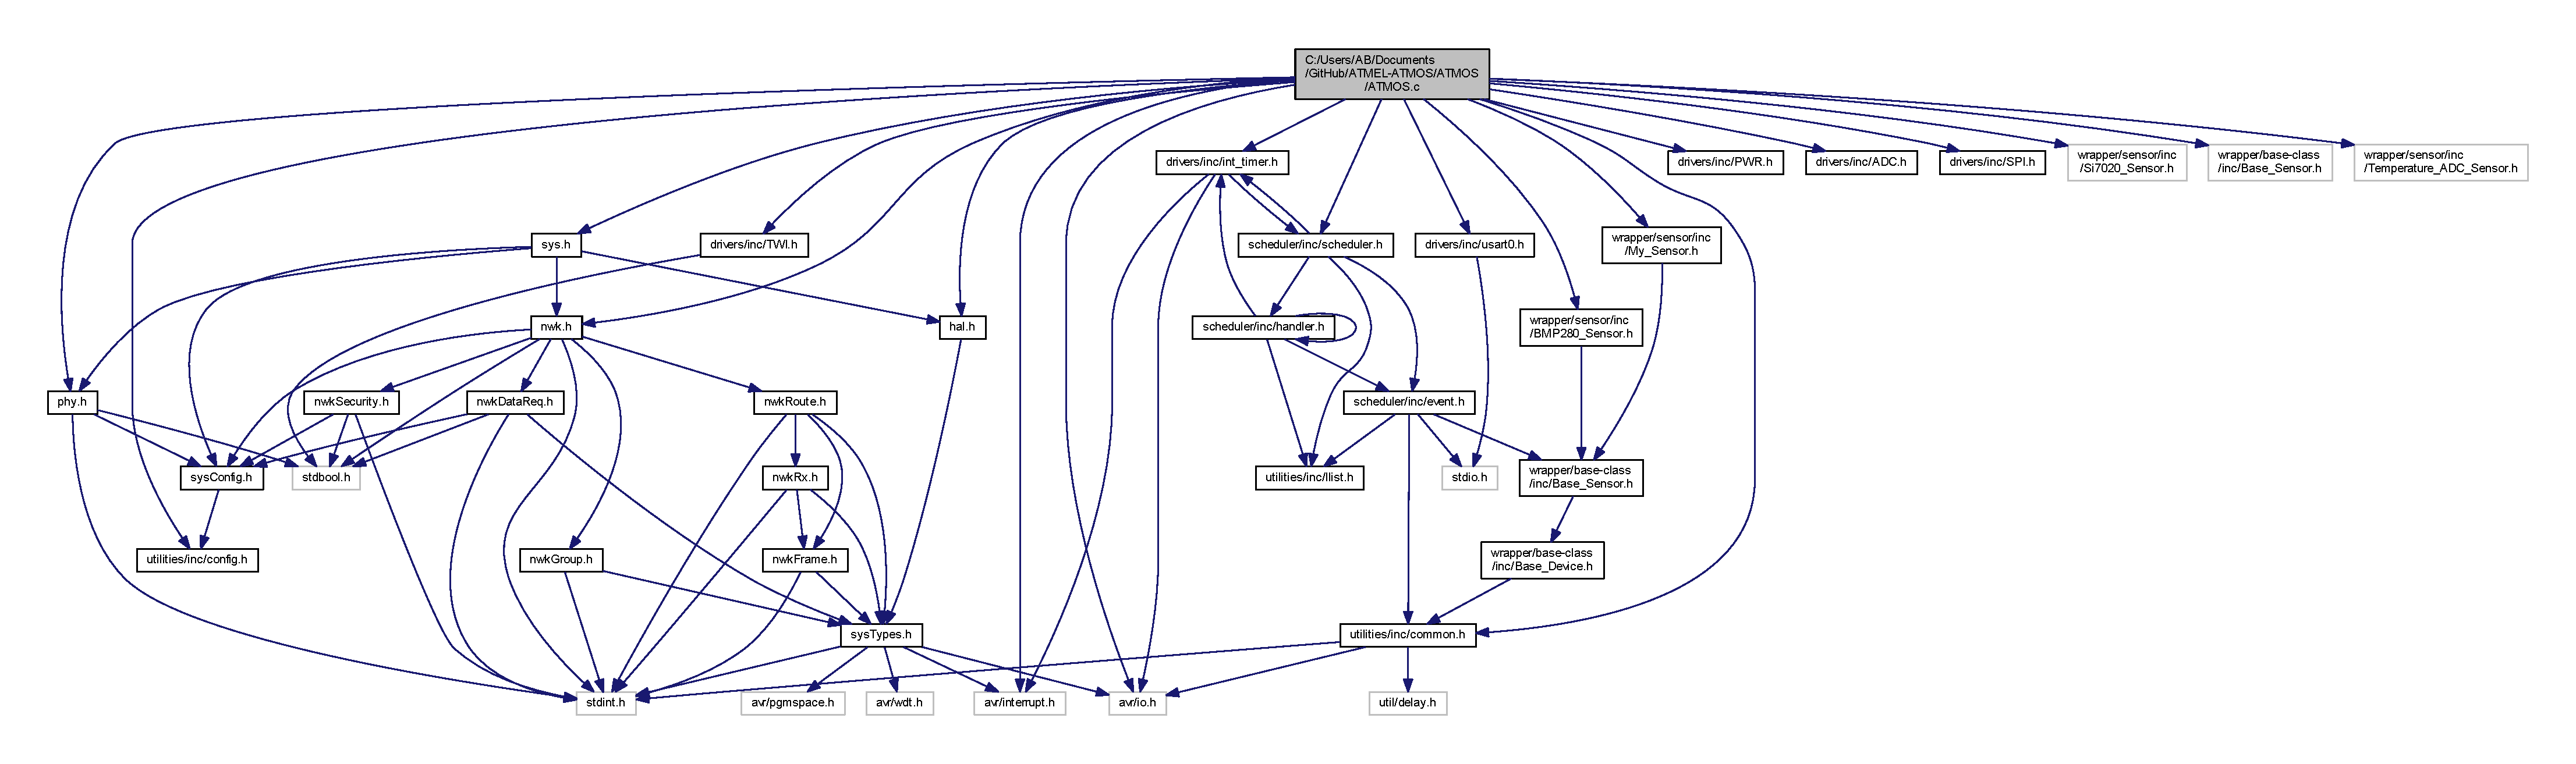
\includegraphics[width=350pt]{_a_t_m_o_s_8c__incl}
\end{center}
\end{figure}
\subsection*{Functions}
\begin{DoxyCompactItemize}
\item 
static void \hyperlink{_a_t_m_o_s_8c_adc8ec6db76d813f9160b2d2933219b29}{A\-P\-P\-\_\-\-Init} (void)
\item 
int \hyperlink{_a_t_m_o_s_8c_a840291bc02cba5474a4cb46a9b9566fe}{main} (void)
\end{DoxyCompactItemize}


\subsection{Detailed Description}
The entry function. 

\subsection{Function Documentation}
\hypertarget{_a_t_m_o_s_8c_adc8ec6db76d813f9160b2d2933219b29}{\index{A\-T\-M\-O\-S.\-c@{A\-T\-M\-O\-S.\-c}!A\-P\-P\-\_\-\-Init@{A\-P\-P\-\_\-\-Init}}
\index{A\-P\-P\-\_\-\-Init@{A\-P\-P\-\_\-\-Init}!ATMOS.c@{A\-T\-M\-O\-S.\-c}}
\subsubsection[{A\-P\-P\-\_\-\-Init}]{\setlength{\rightskip}{0pt plus 5cm}static void A\-P\-P\-\_\-\-Init (
\begin{DoxyParamCaption}
\item[{void}]{}
\end{DoxyParamCaption}
)\hspace{0.3cm}{\ttfamily [static]}}}\label{_a_t_m_o_s_8c_adc8ec6db76d813f9160b2d2933219b29}


References A\-D\-C\-\_\-\-Init(), B\-M\-P280\-\_\-\-Init(), B\-M\-P280\-\_\-\-Set\-Oversampling(), P\-W\-R\-\_\-\-Init(), P\-W\-R\-\_\-\-Turn\-On5\-V(), S\-P\-I\-\_\-\-Slave\-Init(), T\-W\-I\-\_\-\-Init(), and U\-S\-A\-R\-T0\-\_\-\-Init().



Referenced by main().



Here is the call graph for this function\-:
\nopagebreak
\begin{figure}[H]
\begin{center}
\leavevmode
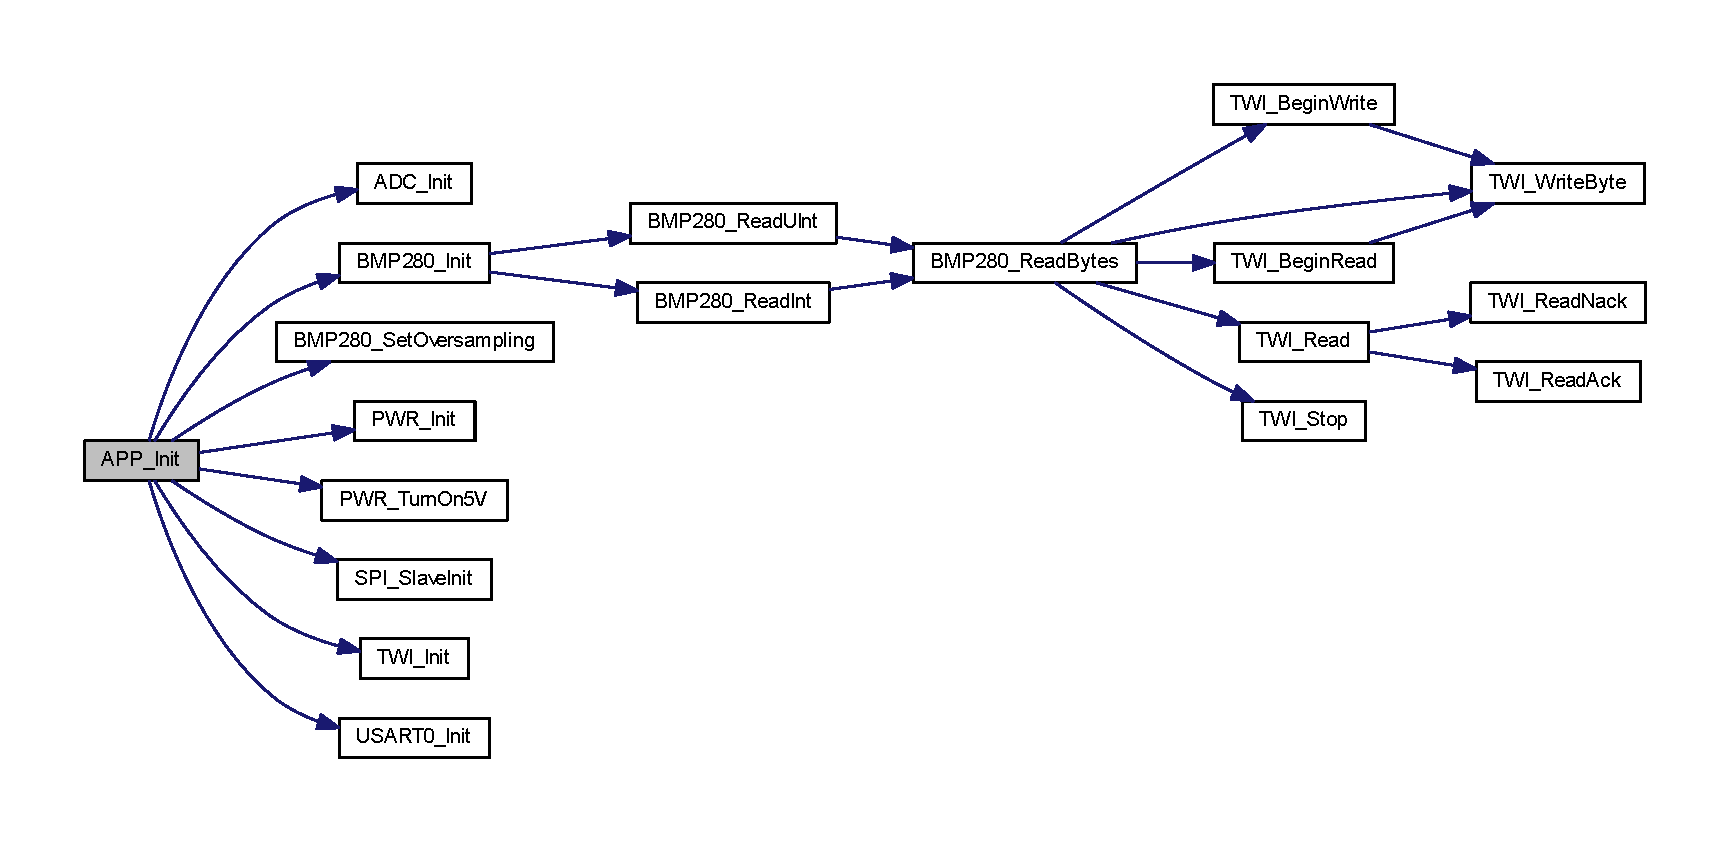
\includegraphics[width=350pt]{_a_t_m_o_s_8c_adc8ec6db76d813f9160b2d2933219b29_cgraph}
\end{center}
\end{figure}




Here is the caller graph for this function\-:
\nopagebreak
\begin{figure}[H]
\begin{center}
\leavevmode
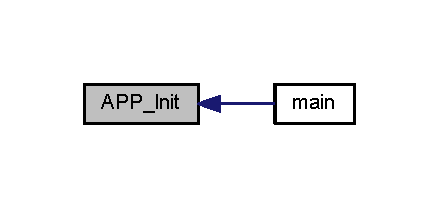
\includegraphics[width=210pt]{_a_t_m_o_s_8c_adc8ec6db76d813f9160b2d2933219b29_icgraph}
\end{center}
\end{figure}


\hypertarget{_a_t_m_o_s_8c_a840291bc02cba5474a4cb46a9b9566fe}{\index{A\-T\-M\-O\-S.\-c@{A\-T\-M\-O\-S.\-c}!main@{main}}
\index{main@{main}!ATMOS.c@{A\-T\-M\-O\-S.\-c}}
\subsubsection[{main}]{\setlength{\rightskip}{0pt plus 5cm}int main (
\begin{DoxyParamCaption}
\item[{void}]{}
\end{DoxyParamCaption}
)}}\label{_a_t_m_o_s_8c_a840291bc02cba5474a4cb46a9b9566fe}


References A\-P\-P\-\_\-\-Init(), B\-M\-P280\-\_\-\-Fctn\-Init(), get\-\_\-next\-\_\-interval(), init\-\_\-\-Event\-\_\-\-Timer(), init\-\_\-set\-\_\-timer(), init\-\_\-timeoutq(), load\-\_\-new\-\_\-sensor(), New\-\_\-\-B\-M\-P280\-\_\-\-Sensor(), and S\-Y\-S\-\_\-\-Init().



Here is the call graph for this function\-:
\nopagebreak
\begin{figure}[H]
\begin{center}
\leavevmode
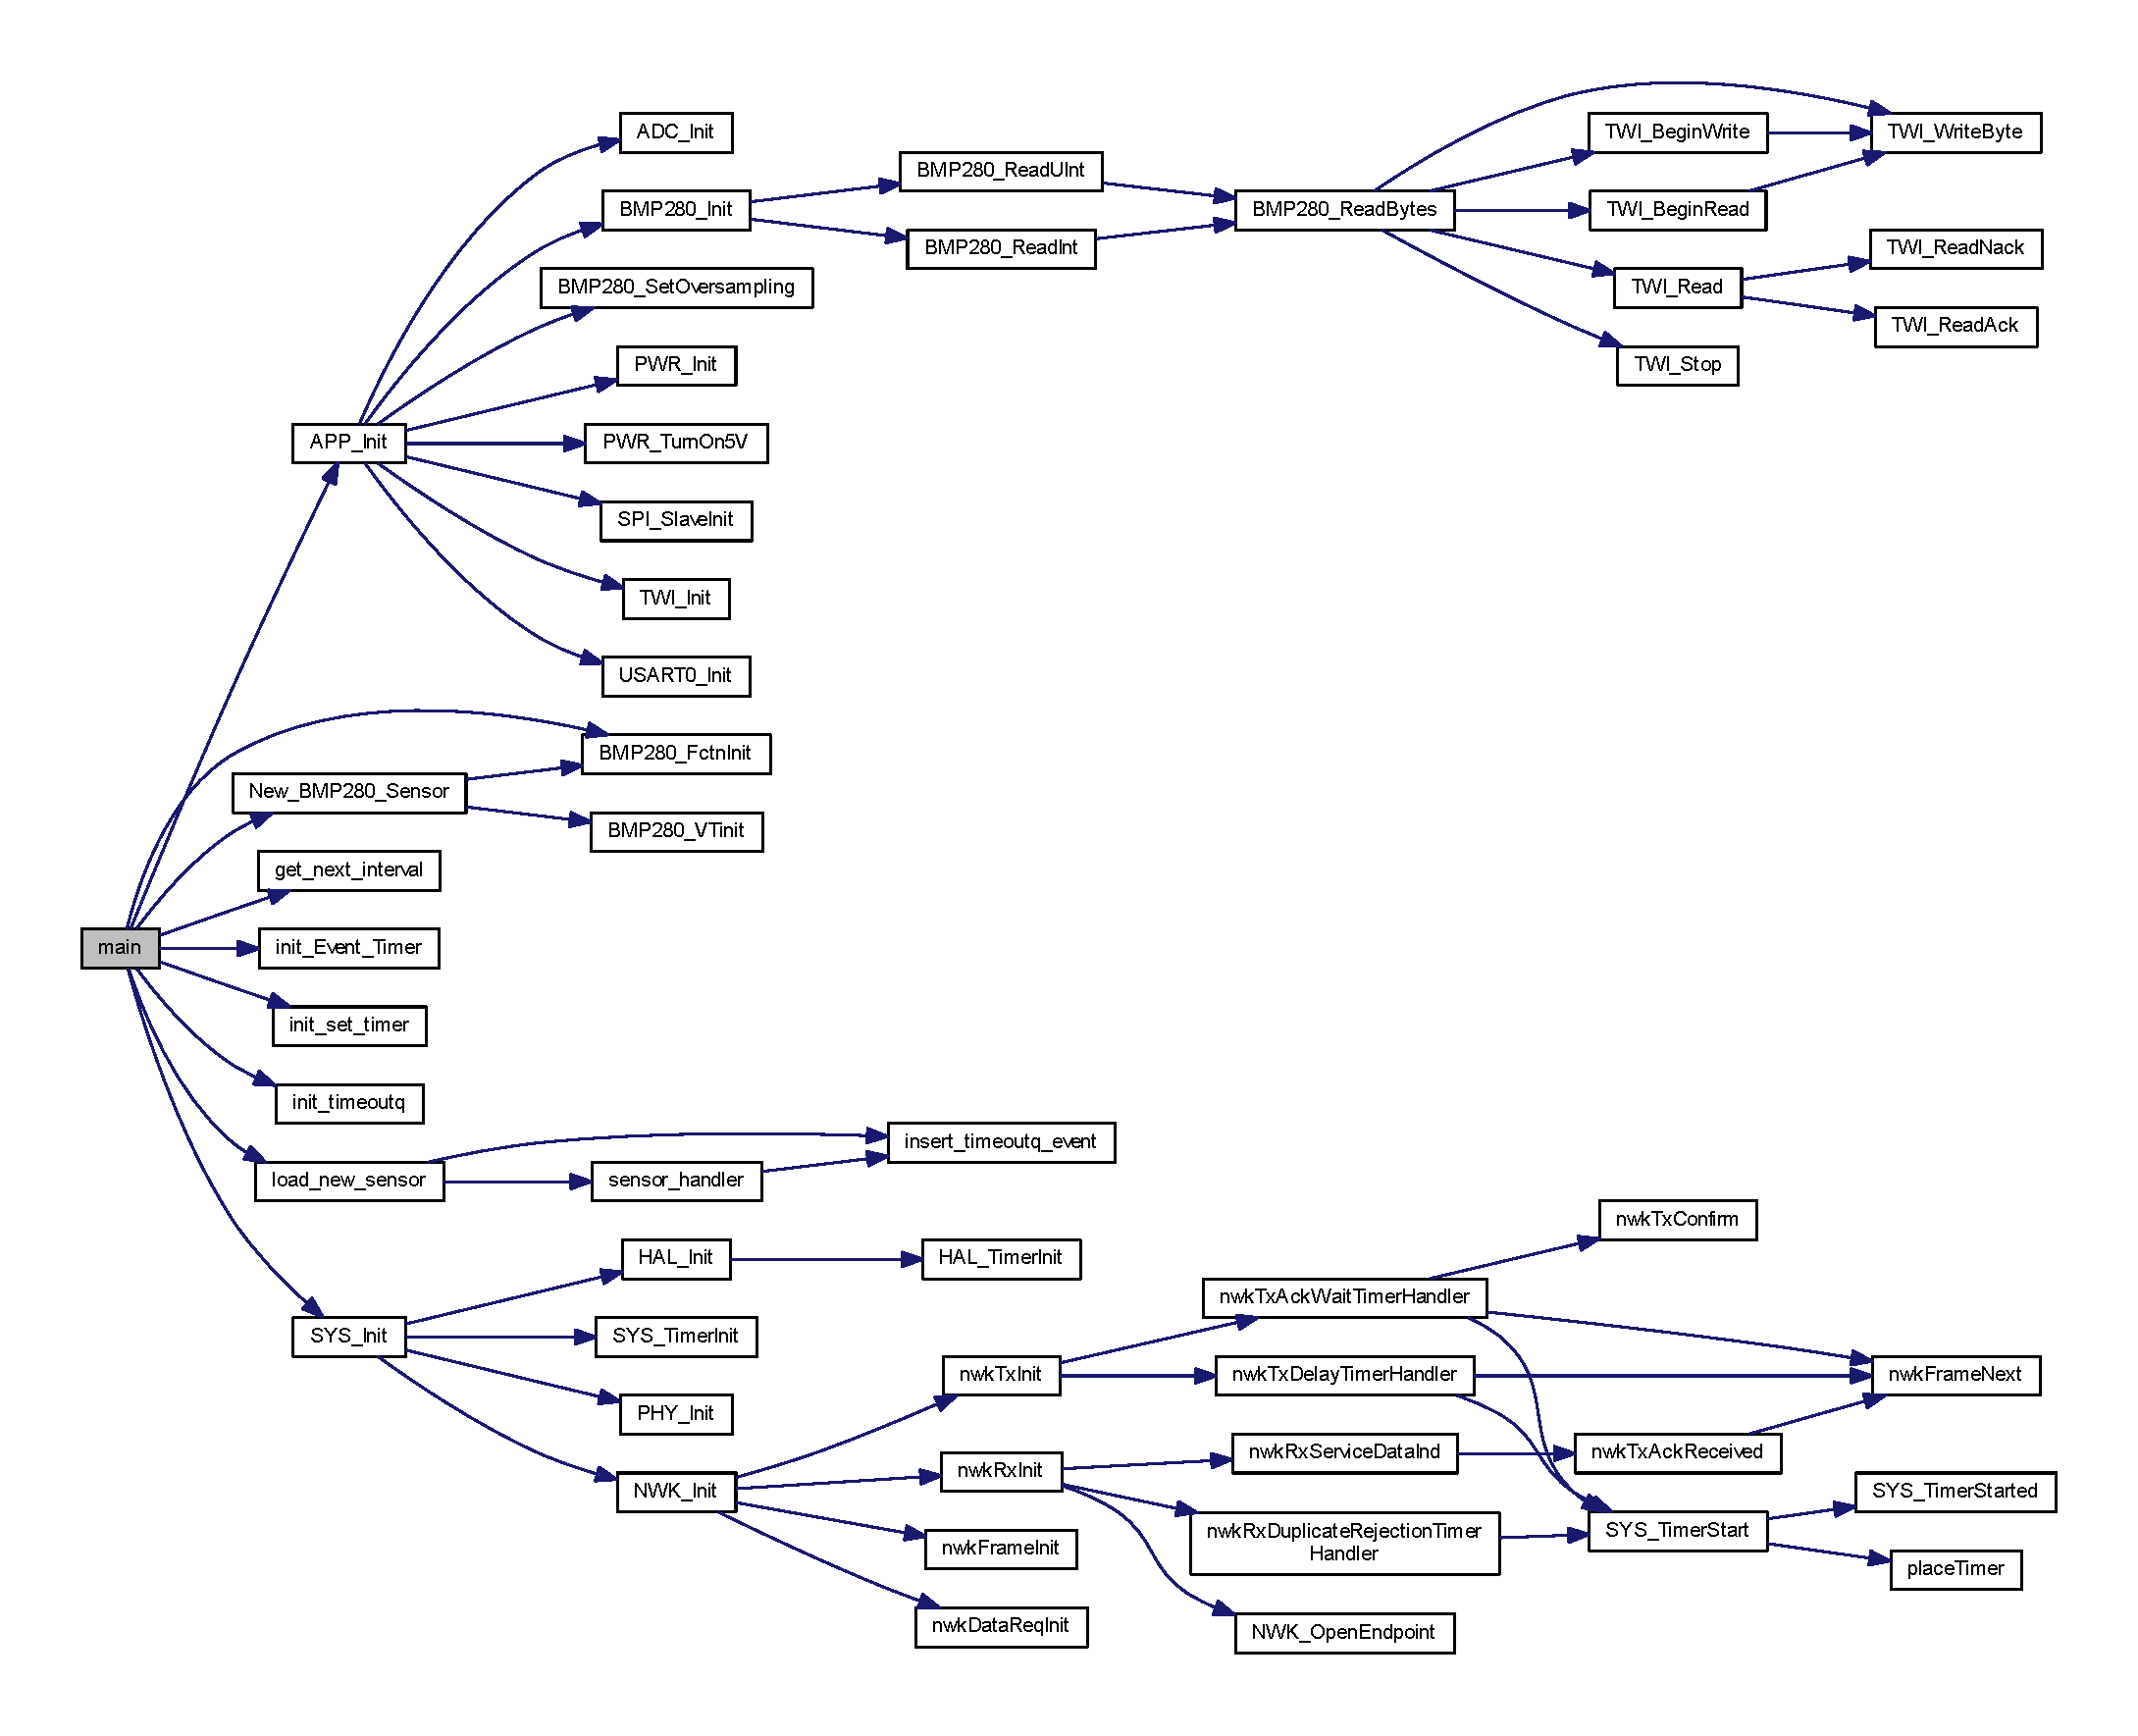
\includegraphics[width=350pt]{_a_t_m_o_s_8c_a840291bc02cba5474a4cb46a9b9566fe_cgraph}
\end{center}
\end{figure}



\hypertarget{_b_m_p280_8h}{\section{C\-:/\-Users/\-A\-B/\-Documents/\-Git\-Hub/\-A\-T\-M\-E\-L-\/\-A\-T\-M\-O\-S/\-A\-T\-M\-O\-S/devices/inc/\-B\-M\-P280.h File Reference}
\label{_b_m_p280_8h}\index{C\-:/\-Users/\-A\-B/\-Documents/\-Git\-Hub/\-A\-T\-M\-E\-L-\/\-A\-T\-M\-O\-S/\-A\-T\-M\-O\-S/devices/inc/\-B\-M\-P280.\-h@{C\-:/\-Users/\-A\-B/\-Documents/\-Git\-Hub/\-A\-T\-M\-E\-L-\/\-A\-T\-M\-O\-S/\-A\-T\-M\-O\-S/devices/inc/\-B\-M\-P280.\-h}}
}


B\-M\-P280 Interface Library.  


{\ttfamily \#include $<$stdbool.\-h$>$}\\*
Include dependency graph for B\-M\-P280.\-h\-:
\nopagebreak
\begin{figure}[H]
\begin{center}
\leavevmode
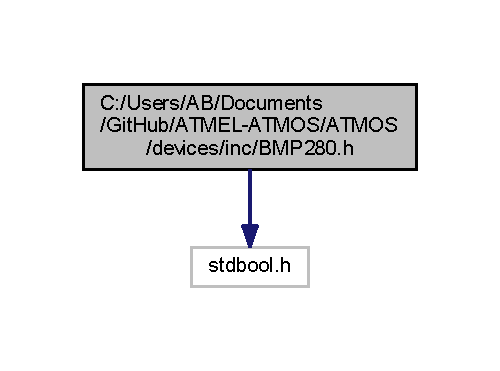
\includegraphics[width=240pt]{_b_m_p280_8h__incl}
\end{center}
\end{figure}
This graph shows which files directly or indirectly include this file\-:
\nopagebreak
\begin{figure}[H]
\begin{center}
\leavevmode
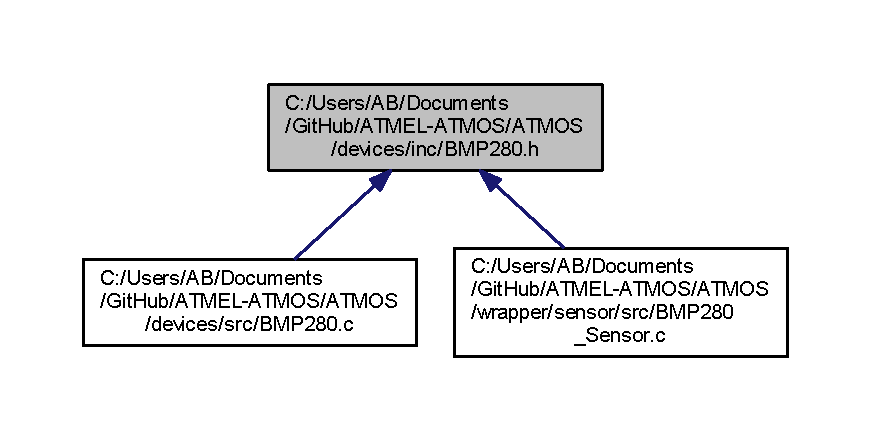
\includegraphics[width=350pt]{_b_m_p280_8h__dep__incl}
\end{center}
\end{figure}
\subsection*{Macros}
\begin{DoxyCompactItemize}
\item 
\#define \hyperlink{_b_m_p280_8h_a64daeac0e223512b505ab0caa06ddbd8}{B\-M\-P280\-\_\-\-A\-D\-D\-R}~0x76
\begin{DoxyCompactList}\small\item\em Device address. \end{DoxyCompactList}\end{DoxyCompactItemize}
\begin{Indent}{\bf T\-W\-I Status Codes}\par
{\em All the codes that could be given via T\-W\-S\-R }\begin{DoxyCompactItemize}
\item 
\#define \hyperlink{_b_m_p280_8h_a72ad9efb996305f741d5ac90bd974454}{B\-M\-P280\-\_\-\-R\-E\-G\-\_\-\-C\-O\-N\-T\-R\-O\-L}~0x\-F4
\item 
\#define \hyperlink{_b_m_p280_8h_a963e6042d8e5635acac0e286157cb6cf}{B\-M\-P280\-\_\-\-R\-E\-G\-\_\-\-R\-E\-S\-U\-L\-T\-\_\-\-P\-R\-E\-S\-S\-U\-R\-E}~0x\-F7
\begin{DoxyCompactList}\small\item\em 0x\-F7(msb) , 0x\-F8(lsb) , 0x\-F9(xlsb) \-: stores the pressure data. \end{DoxyCompactList}\item 
\#define \hyperlink{_b_m_p280_8h_ab34ac559ed33926ad842bd927c2cd04c}{B\-M\-P280\-\_\-\-R\-E\-G\-\_\-\-R\-E\-S\-U\-L\-T\-\_\-\-T\-E\-M\-P\-R\-E\-R\-A\-T\-U\-R\-E}~0x\-F\-A
\begin{DoxyCompactList}\small\item\em 0x\-F\-A(msb) , 0x\-F\-B(lsb) , 0x\-F\-C(xlsb) \-: stores the temperature data. \end{DoxyCompactList}\end{DoxyCompactItemize}
\end{Indent}
\begin{Indent}{\bf Command Macros}\par
{\em Measurement commands to issue to B\-M\-P280\-\_\-\-R\-E\-G\-\_\-\-C\-O\-N\-T\-R\-O\-L }\begin{DoxyCompactItemize}
\item 
\#define \hyperlink{_b_m_p280_8h_a5fa6fe8a5113801977e4e65484d7f461}{B\-M\-P280\-\_\-\-C\-O\-M\-M\-A\-N\-D\-\_\-\-T\-E\-M\-P\-E\-R\-A\-T\-U\-R\-E}~0x2\-E
\item 
\#define \hyperlink{_b_m_p280_8h_a3b86f2a5c89dacf802c6056734fa3976}{B\-M\-P280\-\_\-\-C\-O\-M\-M\-A\-N\-D\-\_\-\-P\-R\-E\-S\-S\-U\-R\-E0}~0x25
\item 
\#define \hyperlink{_b_m_p280_8h_af61c27793531f002244f3a1aa16ca280}{B\-M\-P280\-\_\-\-C\-O\-M\-M\-A\-N\-D\-\_\-\-P\-R\-E\-S\-S\-U\-R\-E1}~0x29
\item 
\#define \hyperlink{_b_m_p280_8h_af336cfa825ec8ca06fdf6ee85d5bda7a}{B\-M\-P280\-\_\-\-C\-O\-M\-M\-A\-N\-D\-\_\-\-P\-R\-E\-S\-S\-U\-R\-E2}~0x2\-D
\item 
\#define \hyperlink{_b_m_p280_8h_a407d2849ebecd8a77bcf2f66bf62c271}{B\-M\-P280\-\_\-\-C\-O\-M\-M\-A\-N\-D\-\_\-\-P\-R\-E\-S\-S\-U\-R\-E3}~0x31
\item 
\#define \hyperlink{_b_m_p280_8h_ae6fab8592a44231f67330303c108c031}{B\-M\-P280\-\_\-\-C\-O\-M\-M\-A\-N\-D\-\_\-\-P\-R\-E\-S\-S\-U\-R\-E4}~0x5\-D
\end{DoxyCompactItemize}
\end{Indent}
\subsection*{Functions}
\begin{DoxyCompactItemize}
\item 
char \hyperlink{_b_m_p280_8h_a2d512d05a3f329da6e0bfb081a1f6685}{B\-M\-P280\-\_\-\-Init} (void)
\begin{DoxyCompactList}\small\item\em Initializes the B\-M\-P280 and reads the calibration data from the device. \end{DoxyCompactList}\item 
char \hyperlink{_b_m_p280_8h_a3aeeb100ef682ba3a48ea93ac87df141}{B\-M\-P280\-\_\-\-Get\-Un\-P\-T} (double $\ast$, double $\ast$)
\begin{DoxyCompactList}\small\item\em Gets the uncalibrated temperature and pressure data. \end{DoxyCompactList}\item 
short \hyperlink{_b_m_p280_8h_a3af5a29c8b539b09126c1dd874a7e6c4}{B\-M\-P280\-\_\-\-Get\-Oversampling} (void)
\begin{DoxyCompactList}\small\item\em Gets the oversampling setting for the library. \end{DoxyCompactList}\item 
char \hyperlink{_b_m_p280_8h_ac56b30a97fa1388153530bb658a0ab3d}{B\-M\-P280\-\_\-\-Set\-Oversampling} (short oss)
\begin{DoxyCompactList}\small\item\em Sets the oversampling setting for the library. \end{DoxyCompactList}\item 
char \hyperlink{_b_m_p280_8h_a79fe54e0ce75dc946a3540bddd43e878}{B\-M\-P280\-\_\-\-Start\-Measurment} (void)
\begin{DoxyCompactList}\small\item\em Starts a measurement. \end{DoxyCompactList}\item 
char \hyperlink{_b_m_p280_8h_aab0220cf4e61916eedbc1d5f72495c86}{B\-M\-P280\-\_\-\-Get\-Temperature\-And\-Pressure} (double $\ast$, double $\ast$)
\begin{DoxyCompactList}\small\item\em Gets temperature and pressure. \end{DoxyCompactList}\item 
char \hyperlink{_b_m_p280_8h_ac8c6848873b9fed4010c5c4f472a4ae2}{B\-M\-P280\-\_\-\-Calc\-Temperature} (double $\ast$, double $\ast$)
\begin{DoxyCompactList}\small\item\em Calculates temperature. \end{DoxyCompactList}\item 
char \hyperlink{_b_m_p280_8h_a782bc0a3fa2ac03ae179edb89bf91726}{B\-M\-P280\-\_\-\-Calc\-Pressure} (double $\ast$, double $\ast$)
\begin{DoxyCompactList}\small\item\em Calculates pressure. \end{DoxyCompactList}\item 
double \hyperlink{_b_m_p280_8h_acfd338e24de5158c7ec8389d6c4eaa6a}{B\-M\-P280\-\_\-\-Sealevel} (double, double)
\begin{DoxyCompactList}\small\item\em Calculates pressure at sea level given an altitude. \end{DoxyCompactList}\item 
double \hyperlink{_b_m_p280_8h_a109695e8464300cb4ec8593289627c93}{B\-M\-P280\-\_\-\-Altitude} (double, double)
\begin{DoxyCompactList}\small\item\em Calculates altitude. \end{DoxyCompactList}\item 
char \hyperlink{_b_m_p280_8h_aeca60c0f36d134193d76793f85476422}{B\-M\-P280\-\_\-\-Get\-Error} (void)
\begin{DoxyCompactList}\small\item\em Returns the internal library error value. \end{DoxyCompactList}\end{DoxyCompactItemize}


\subsection{Detailed Description}
B\-M\-P280 Interface Library. Created\-: 2/10/2015 20\-:25\-:27 Author\-: Camden Miller 

\subsection{Macro Definition Documentation}
\hypertarget{_b_m_p280_8h_a64daeac0e223512b505ab0caa06ddbd8}{\index{B\-M\-P280.\-h@{B\-M\-P280.\-h}!B\-M\-P280\-\_\-\-A\-D\-D\-R@{B\-M\-P280\-\_\-\-A\-D\-D\-R}}
\index{B\-M\-P280\-\_\-\-A\-D\-D\-R@{B\-M\-P280\-\_\-\-A\-D\-D\-R}!BMP280.h@{B\-M\-P280.\-h}}
\subsubsection[{B\-M\-P280\-\_\-\-A\-D\-D\-R}]{\setlength{\rightskip}{0pt plus 5cm}\#define B\-M\-P280\-\_\-\-A\-D\-D\-R~0x76}}\label{_b_m_p280_8h_a64daeac0e223512b505ab0caa06ddbd8}


Device address. 



Referenced by B\-M\-P280\-\_\-\-Read\-Bytes(), and B\-M\-P280\-\_\-\-Write\-Bytes().

\hypertarget{_b_m_p280_8h_a3b86f2a5c89dacf802c6056734fa3976}{\index{B\-M\-P280.\-h@{B\-M\-P280.\-h}!B\-M\-P280\-\_\-\-C\-O\-M\-M\-A\-N\-D\-\_\-\-P\-R\-E\-S\-S\-U\-R\-E0@{B\-M\-P280\-\_\-\-C\-O\-M\-M\-A\-N\-D\-\_\-\-P\-R\-E\-S\-S\-U\-R\-E0}}
\index{B\-M\-P280\-\_\-\-C\-O\-M\-M\-A\-N\-D\-\_\-\-P\-R\-E\-S\-S\-U\-R\-E0@{B\-M\-P280\-\_\-\-C\-O\-M\-M\-A\-N\-D\-\_\-\-P\-R\-E\-S\-S\-U\-R\-E0}!BMP280.h@{B\-M\-P280.\-h}}
\subsubsection[{B\-M\-P280\-\_\-\-C\-O\-M\-M\-A\-N\-D\-\_\-\-P\-R\-E\-S\-S\-U\-R\-E0}]{\setlength{\rightskip}{0pt plus 5cm}\#define B\-M\-P280\-\_\-\-C\-O\-M\-M\-A\-N\-D\-\_\-\-P\-R\-E\-S\-S\-U\-R\-E0~0x25}}\label{_b_m_p280_8h_a3b86f2a5c89dacf802c6056734fa3976}


Referenced by B\-M\-P280\-\_\-\-Start\-Measurment().

\hypertarget{_b_m_p280_8h_af61c27793531f002244f3a1aa16ca280}{\index{B\-M\-P280.\-h@{B\-M\-P280.\-h}!B\-M\-P280\-\_\-\-C\-O\-M\-M\-A\-N\-D\-\_\-\-P\-R\-E\-S\-S\-U\-R\-E1@{B\-M\-P280\-\_\-\-C\-O\-M\-M\-A\-N\-D\-\_\-\-P\-R\-E\-S\-S\-U\-R\-E1}}
\index{B\-M\-P280\-\_\-\-C\-O\-M\-M\-A\-N\-D\-\_\-\-P\-R\-E\-S\-S\-U\-R\-E1@{B\-M\-P280\-\_\-\-C\-O\-M\-M\-A\-N\-D\-\_\-\-P\-R\-E\-S\-S\-U\-R\-E1}!BMP280.h@{B\-M\-P280.\-h}}
\subsubsection[{B\-M\-P280\-\_\-\-C\-O\-M\-M\-A\-N\-D\-\_\-\-P\-R\-E\-S\-S\-U\-R\-E1}]{\setlength{\rightskip}{0pt plus 5cm}\#define B\-M\-P280\-\_\-\-C\-O\-M\-M\-A\-N\-D\-\_\-\-P\-R\-E\-S\-S\-U\-R\-E1~0x29}}\label{_b_m_p280_8h_af61c27793531f002244f3a1aa16ca280}


Referenced by B\-M\-P280\-\_\-\-Start\-Measurment().

\hypertarget{_b_m_p280_8h_af336cfa825ec8ca06fdf6ee85d5bda7a}{\index{B\-M\-P280.\-h@{B\-M\-P280.\-h}!B\-M\-P280\-\_\-\-C\-O\-M\-M\-A\-N\-D\-\_\-\-P\-R\-E\-S\-S\-U\-R\-E2@{B\-M\-P280\-\_\-\-C\-O\-M\-M\-A\-N\-D\-\_\-\-P\-R\-E\-S\-S\-U\-R\-E2}}
\index{B\-M\-P280\-\_\-\-C\-O\-M\-M\-A\-N\-D\-\_\-\-P\-R\-E\-S\-S\-U\-R\-E2@{B\-M\-P280\-\_\-\-C\-O\-M\-M\-A\-N\-D\-\_\-\-P\-R\-E\-S\-S\-U\-R\-E2}!BMP280.h@{B\-M\-P280.\-h}}
\subsubsection[{B\-M\-P280\-\_\-\-C\-O\-M\-M\-A\-N\-D\-\_\-\-P\-R\-E\-S\-S\-U\-R\-E2}]{\setlength{\rightskip}{0pt plus 5cm}\#define B\-M\-P280\-\_\-\-C\-O\-M\-M\-A\-N\-D\-\_\-\-P\-R\-E\-S\-S\-U\-R\-E2~0x2\-D}}\label{_b_m_p280_8h_af336cfa825ec8ca06fdf6ee85d5bda7a}


Referenced by B\-M\-P280\-\_\-\-Start\-Measurment().

\hypertarget{_b_m_p280_8h_a407d2849ebecd8a77bcf2f66bf62c271}{\index{B\-M\-P280.\-h@{B\-M\-P280.\-h}!B\-M\-P280\-\_\-\-C\-O\-M\-M\-A\-N\-D\-\_\-\-P\-R\-E\-S\-S\-U\-R\-E3@{B\-M\-P280\-\_\-\-C\-O\-M\-M\-A\-N\-D\-\_\-\-P\-R\-E\-S\-S\-U\-R\-E3}}
\index{B\-M\-P280\-\_\-\-C\-O\-M\-M\-A\-N\-D\-\_\-\-P\-R\-E\-S\-S\-U\-R\-E3@{B\-M\-P280\-\_\-\-C\-O\-M\-M\-A\-N\-D\-\_\-\-P\-R\-E\-S\-S\-U\-R\-E3}!BMP280.h@{B\-M\-P280.\-h}}
\subsubsection[{B\-M\-P280\-\_\-\-C\-O\-M\-M\-A\-N\-D\-\_\-\-P\-R\-E\-S\-S\-U\-R\-E3}]{\setlength{\rightskip}{0pt plus 5cm}\#define B\-M\-P280\-\_\-\-C\-O\-M\-M\-A\-N\-D\-\_\-\-P\-R\-E\-S\-S\-U\-R\-E3~0x31}}\label{_b_m_p280_8h_a407d2849ebecd8a77bcf2f66bf62c271}


Referenced by B\-M\-P280\-\_\-\-Start\-Measurment().

\hypertarget{_b_m_p280_8h_ae6fab8592a44231f67330303c108c031}{\index{B\-M\-P280.\-h@{B\-M\-P280.\-h}!B\-M\-P280\-\_\-\-C\-O\-M\-M\-A\-N\-D\-\_\-\-P\-R\-E\-S\-S\-U\-R\-E4@{B\-M\-P280\-\_\-\-C\-O\-M\-M\-A\-N\-D\-\_\-\-P\-R\-E\-S\-S\-U\-R\-E4}}
\index{B\-M\-P280\-\_\-\-C\-O\-M\-M\-A\-N\-D\-\_\-\-P\-R\-E\-S\-S\-U\-R\-E4@{B\-M\-P280\-\_\-\-C\-O\-M\-M\-A\-N\-D\-\_\-\-P\-R\-E\-S\-S\-U\-R\-E4}!BMP280.h@{B\-M\-P280.\-h}}
\subsubsection[{B\-M\-P280\-\_\-\-C\-O\-M\-M\-A\-N\-D\-\_\-\-P\-R\-E\-S\-S\-U\-R\-E4}]{\setlength{\rightskip}{0pt plus 5cm}\#define B\-M\-P280\-\_\-\-C\-O\-M\-M\-A\-N\-D\-\_\-\-P\-R\-E\-S\-S\-U\-R\-E4~0x5\-D}}\label{_b_m_p280_8h_ae6fab8592a44231f67330303c108c031}


Referenced by B\-M\-P280\-\_\-\-Start\-Measurment().

\hypertarget{_b_m_p280_8h_a5fa6fe8a5113801977e4e65484d7f461}{\index{B\-M\-P280.\-h@{B\-M\-P280.\-h}!B\-M\-P280\-\_\-\-C\-O\-M\-M\-A\-N\-D\-\_\-\-T\-E\-M\-P\-E\-R\-A\-T\-U\-R\-E@{B\-M\-P280\-\_\-\-C\-O\-M\-M\-A\-N\-D\-\_\-\-T\-E\-M\-P\-E\-R\-A\-T\-U\-R\-E}}
\index{B\-M\-P280\-\_\-\-C\-O\-M\-M\-A\-N\-D\-\_\-\-T\-E\-M\-P\-E\-R\-A\-T\-U\-R\-E@{B\-M\-P280\-\_\-\-C\-O\-M\-M\-A\-N\-D\-\_\-\-T\-E\-M\-P\-E\-R\-A\-T\-U\-R\-E}!BMP280.h@{B\-M\-P280.\-h}}
\subsubsection[{B\-M\-P280\-\_\-\-C\-O\-M\-M\-A\-N\-D\-\_\-\-T\-E\-M\-P\-E\-R\-A\-T\-U\-R\-E}]{\setlength{\rightskip}{0pt plus 5cm}\#define B\-M\-P280\-\_\-\-C\-O\-M\-M\-A\-N\-D\-\_\-\-T\-E\-M\-P\-E\-R\-A\-T\-U\-R\-E~0x2\-E}}\label{_b_m_p280_8h_a5fa6fe8a5113801977e4e65484d7f461}
\hypertarget{_b_m_p280_8h_a72ad9efb996305f741d5ac90bd974454}{\index{B\-M\-P280.\-h@{B\-M\-P280.\-h}!B\-M\-P280\-\_\-\-R\-E\-G\-\_\-\-C\-O\-N\-T\-R\-O\-L@{B\-M\-P280\-\_\-\-R\-E\-G\-\_\-\-C\-O\-N\-T\-R\-O\-L}}
\index{B\-M\-P280\-\_\-\-R\-E\-G\-\_\-\-C\-O\-N\-T\-R\-O\-L@{B\-M\-P280\-\_\-\-R\-E\-G\-\_\-\-C\-O\-N\-T\-R\-O\-L}!BMP280.h@{B\-M\-P280.\-h}}
\subsubsection[{B\-M\-P280\-\_\-\-R\-E\-G\-\_\-\-C\-O\-N\-T\-R\-O\-L}]{\setlength{\rightskip}{0pt plus 5cm}\#define B\-M\-P280\-\_\-\-R\-E\-G\-\_\-\-C\-O\-N\-T\-R\-O\-L~0x\-F4}}\label{_b_m_p280_8h_a72ad9efb996305f741d5ac90bd974454}


Referenced by B\-M\-P280\-\_\-\-Start\-Measurment().

\hypertarget{_b_m_p280_8h_a963e6042d8e5635acac0e286157cb6cf}{\index{B\-M\-P280.\-h@{B\-M\-P280.\-h}!B\-M\-P280\-\_\-\-R\-E\-G\-\_\-\-R\-E\-S\-U\-L\-T\-\_\-\-P\-R\-E\-S\-S\-U\-R\-E@{B\-M\-P280\-\_\-\-R\-E\-G\-\_\-\-R\-E\-S\-U\-L\-T\-\_\-\-P\-R\-E\-S\-S\-U\-R\-E}}
\index{B\-M\-P280\-\_\-\-R\-E\-G\-\_\-\-R\-E\-S\-U\-L\-T\-\_\-\-P\-R\-E\-S\-S\-U\-R\-E@{B\-M\-P280\-\_\-\-R\-E\-G\-\_\-\-R\-E\-S\-U\-L\-T\-\_\-\-P\-R\-E\-S\-S\-U\-R\-E}!BMP280.h@{B\-M\-P280.\-h}}
\subsubsection[{B\-M\-P280\-\_\-\-R\-E\-G\-\_\-\-R\-E\-S\-U\-L\-T\-\_\-\-P\-R\-E\-S\-S\-U\-R\-E}]{\setlength{\rightskip}{0pt plus 5cm}\#define B\-M\-P280\-\_\-\-R\-E\-G\-\_\-\-R\-E\-S\-U\-L\-T\-\_\-\-P\-R\-E\-S\-S\-U\-R\-E~0x\-F7}}\label{_b_m_p280_8h_a963e6042d8e5635acac0e286157cb6cf}


0x\-F7(msb) , 0x\-F8(lsb) , 0x\-F9(xlsb) \-: stores the pressure data. 



Referenced by B\-M\-P280\-\_\-\-Get\-Un\-P\-T().

\hypertarget{_b_m_p280_8h_ab34ac559ed33926ad842bd927c2cd04c}{\index{B\-M\-P280.\-h@{B\-M\-P280.\-h}!B\-M\-P280\-\_\-\-R\-E\-G\-\_\-\-R\-E\-S\-U\-L\-T\-\_\-\-T\-E\-M\-P\-R\-E\-R\-A\-T\-U\-R\-E@{B\-M\-P280\-\_\-\-R\-E\-G\-\_\-\-R\-E\-S\-U\-L\-T\-\_\-\-T\-E\-M\-P\-R\-E\-R\-A\-T\-U\-R\-E}}
\index{B\-M\-P280\-\_\-\-R\-E\-G\-\_\-\-R\-E\-S\-U\-L\-T\-\_\-\-T\-E\-M\-P\-R\-E\-R\-A\-T\-U\-R\-E@{B\-M\-P280\-\_\-\-R\-E\-G\-\_\-\-R\-E\-S\-U\-L\-T\-\_\-\-T\-E\-M\-P\-R\-E\-R\-A\-T\-U\-R\-E}!BMP280.h@{B\-M\-P280.\-h}}
\subsubsection[{B\-M\-P280\-\_\-\-R\-E\-G\-\_\-\-R\-E\-S\-U\-L\-T\-\_\-\-T\-E\-M\-P\-R\-E\-R\-A\-T\-U\-R\-E}]{\setlength{\rightskip}{0pt plus 5cm}\#define B\-M\-P280\-\_\-\-R\-E\-G\-\_\-\-R\-E\-S\-U\-L\-T\-\_\-\-T\-E\-M\-P\-R\-E\-R\-A\-T\-U\-R\-E~0x\-F\-A}}\label{_b_m_p280_8h_ab34ac559ed33926ad842bd927c2cd04c}


0x\-F\-A(msb) , 0x\-F\-B(lsb) , 0x\-F\-C(xlsb) \-: stores the temperature data. 



\subsection{Function Documentation}
\hypertarget{_b_m_p280_8h_a109695e8464300cb4ec8593289627c93}{\index{B\-M\-P280.\-h@{B\-M\-P280.\-h}!B\-M\-P280\-\_\-\-Altitude@{B\-M\-P280\-\_\-\-Altitude}}
\index{B\-M\-P280\-\_\-\-Altitude@{B\-M\-P280\-\_\-\-Altitude}!BMP280.h@{B\-M\-P280.\-h}}
\subsubsection[{B\-M\-P280\-\_\-\-Altitude}]{\setlength{\rightskip}{0pt plus 5cm}double B\-M\-P280\-\_\-\-Altitude (
\begin{DoxyParamCaption}
\item[{double}]{P, }
\item[{double}]{P0}
\end{DoxyParamCaption}
)}}\label{_b_m_p280_8h_a109695e8464300cb4ec8593289627c93}


Calculates altitude. 


\begin{DoxyParams}[1]{Parameters}
\mbox{\tt in}  & {\em pressure} & reading \\
\hline
\mbox{\tt in}  & {\em sea} & level pressure \\
\hline
\end{DoxyParams}
\begin{DoxyReturn}{Returns}
the corrected reading 
\end{DoxyReturn}
\hypertarget{_b_m_p280_8h_a782bc0a3fa2ac03ae179edb89bf91726}{\index{B\-M\-P280.\-h@{B\-M\-P280.\-h}!B\-M\-P280\-\_\-\-Calc\-Pressure@{B\-M\-P280\-\_\-\-Calc\-Pressure}}
\index{B\-M\-P280\-\_\-\-Calc\-Pressure@{B\-M\-P280\-\_\-\-Calc\-Pressure}!BMP280.h@{B\-M\-P280.\-h}}
\subsubsection[{B\-M\-P280\-\_\-\-Calc\-Pressure}]{\setlength{\rightskip}{0pt plus 5cm}char B\-M\-P280\-\_\-\-Calc\-Pressure (
\begin{DoxyParamCaption}
\item[{double $\ast$}]{P, }
\item[{double $\ast$}]{u\-P}
\end{DoxyParamCaption}
)}}\label{_b_m_p280_8h_a782bc0a3fa2ac03ae179edb89bf91726}


Calculates pressure. 


\begin{DoxyParams}[1]{Parameters}
\mbox{\tt out}  & {\em pointer} & to a place to store the pressure data \\
\hline
\mbox{\tt in}  & {\em pointer} & to the uncalibrated pressure data \\
\hline
\end{DoxyParams}
\begin{DoxyReturn}{Returns}
status 
\end{DoxyReturn}


References dig\-\_\-\-P1, dig\-\_\-\-P2, dig\-\_\-\-P3, dig\-\_\-\-P4, dig\-\_\-\-P5, dig\-\_\-\-P6, dig\-\_\-\-P7, dig\-\_\-\-P8, dig\-\_\-\-P9, and t\-\_\-fine.



Referenced by B\-M\-P280\-\_\-\-Get\-Temperature\-And\-Pressure().



Here is the caller graph for this function\-:
\nopagebreak
\begin{figure}[H]
\begin{center}
\leavevmode
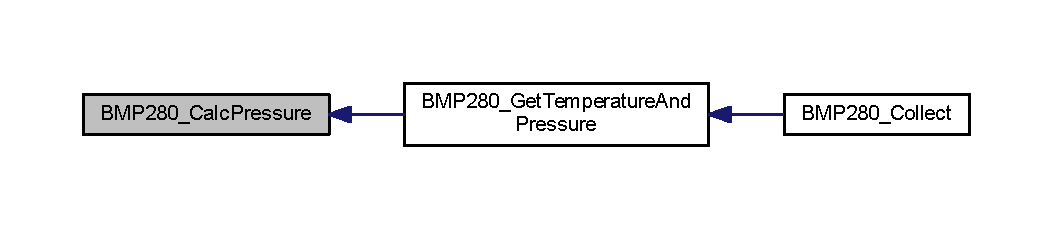
\includegraphics[width=350pt]{_b_m_p280_8h_a782bc0a3fa2ac03ae179edb89bf91726_icgraph}
\end{center}
\end{figure}


\hypertarget{_b_m_p280_8h_ac8c6848873b9fed4010c5c4f472a4ae2}{\index{B\-M\-P280.\-h@{B\-M\-P280.\-h}!B\-M\-P280\-\_\-\-Calc\-Temperature@{B\-M\-P280\-\_\-\-Calc\-Temperature}}
\index{B\-M\-P280\-\_\-\-Calc\-Temperature@{B\-M\-P280\-\_\-\-Calc\-Temperature}!BMP280.h@{B\-M\-P280.\-h}}
\subsubsection[{B\-M\-P280\-\_\-\-Calc\-Temperature}]{\setlength{\rightskip}{0pt plus 5cm}char B\-M\-P280\-\_\-\-Calc\-Temperature (
\begin{DoxyParamCaption}
\item[{double $\ast$}]{T, }
\item[{double $\ast$}]{u\-T}
\end{DoxyParamCaption}
)}}\label{_b_m_p280_8h_ac8c6848873b9fed4010c5c4f472a4ae2}


Calculates temperature. 


\begin{DoxyParams}[1]{Parameters}
\mbox{\tt out}  & {\em pointer} & to a place to store the temperature data \\
\hline
\mbox{\tt in}  & {\em pointer} & to the uncalibrated temperature data \\
\hline
\end{DoxyParams}
\begin{DoxyReturn}{Returns}
status 
\end{DoxyReturn}


References dig\-\_\-\-T1, dig\-\_\-\-T2, dig\-\_\-\-T3, and t\-\_\-fine.



Referenced by B\-M\-P280\-\_\-\-Get\-Temperature\-And\-Pressure().



Here is the caller graph for this function\-:
\nopagebreak
\begin{figure}[H]
\begin{center}
\leavevmode
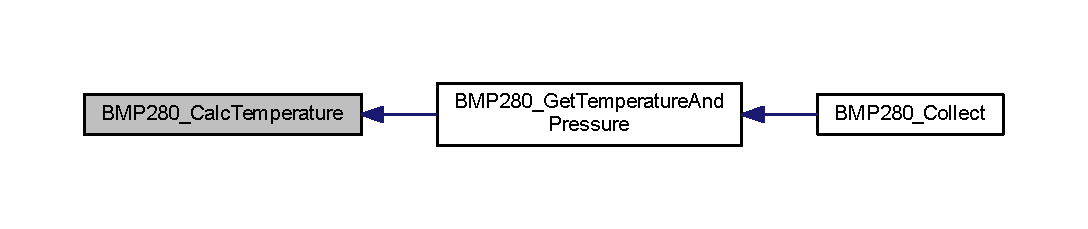
\includegraphics[width=350pt]{_b_m_p280_8h_ac8c6848873b9fed4010c5c4f472a4ae2_icgraph}
\end{center}
\end{figure}


\hypertarget{_b_m_p280_8h_aeca60c0f36d134193d76793f85476422}{\index{B\-M\-P280.\-h@{B\-M\-P280.\-h}!B\-M\-P280\-\_\-\-Get\-Error@{B\-M\-P280\-\_\-\-Get\-Error}}
\index{B\-M\-P280\-\_\-\-Get\-Error@{B\-M\-P280\-\_\-\-Get\-Error}!BMP280.h@{B\-M\-P280.\-h}}
\subsubsection[{B\-M\-P280\-\_\-\-Get\-Error}]{\setlength{\rightskip}{0pt plus 5cm}char B\-M\-P280\-\_\-\-Get\-Error (
\begin{DoxyParamCaption}
\item[{void}]{}
\end{DoxyParamCaption}
)}}\label{_b_m_p280_8h_aeca60c0f36d134193d76793f85476422}


Returns the internal library error value. 


\begin{DoxyParams}[1]{Parameters}
\mbox{\tt in}  & {\em pressure} & reading \\
\hline
\mbox{\tt in}  & {\em sea} & level pressure \\
\hline
\end{DoxyParams}
\begin{DoxyReturn}{Returns}
error value 
\end{DoxyReturn}


References error.

\hypertarget{_b_m_p280_8h_a3af5a29c8b539b09126c1dd874a7e6c4}{\index{B\-M\-P280.\-h@{B\-M\-P280.\-h}!B\-M\-P280\-\_\-\-Get\-Oversampling@{B\-M\-P280\-\_\-\-Get\-Oversampling}}
\index{B\-M\-P280\-\_\-\-Get\-Oversampling@{B\-M\-P280\-\_\-\-Get\-Oversampling}!BMP280.h@{B\-M\-P280.\-h}}
\subsubsection[{B\-M\-P280\-\_\-\-Get\-Oversampling}]{\setlength{\rightskip}{0pt plus 5cm}short B\-M\-P280\-\_\-\-Get\-Oversampling (
\begin{DoxyParamCaption}
\item[{void}]{}
\end{DoxyParamCaption}
)}}\label{_b_m_p280_8h_a3af5a29c8b539b09126c1dd874a7e6c4}


Gets the oversampling setting for the library. 

\begin{DoxyReturn}{Returns}
oversampling 
\end{DoxyReturn}


References oversampling.

\hypertarget{_b_m_p280_8h_aab0220cf4e61916eedbc1d5f72495c86}{\index{B\-M\-P280.\-h@{B\-M\-P280.\-h}!B\-M\-P280\-\_\-\-Get\-Temperature\-And\-Pressure@{B\-M\-P280\-\_\-\-Get\-Temperature\-And\-Pressure}}
\index{B\-M\-P280\-\_\-\-Get\-Temperature\-And\-Pressure@{B\-M\-P280\-\_\-\-Get\-Temperature\-And\-Pressure}!BMP280.h@{B\-M\-P280.\-h}}
\subsubsection[{B\-M\-P280\-\_\-\-Get\-Temperature\-And\-Pressure}]{\setlength{\rightskip}{0pt plus 5cm}char B\-M\-P280\-\_\-\-Get\-Temperature\-And\-Pressure (
\begin{DoxyParamCaption}
\item[{double $\ast$}]{T, }
\item[{double $\ast$}]{P}
\end{DoxyParamCaption}
)}}\label{_b_m_p280_8h_aab0220cf4e61916eedbc1d5f72495c86}


Gets temperature and pressure. 


\begin{DoxyParams}[1]{Parameters}
\mbox{\tt out}  & {\em pointer} & to a place to store the pressure data \\
\hline
\mbox{\tt out}  & {\em pointer} & to a place to store the temperature data \\
\hline
\end{DoxyParams}
\begin{DoxyReturn}{Returns}
status 
\end{DoxyReturn}


References B\-M\-P280\-\_\-\-Calc\-Pressure(), B\-M\-P280\-\_\-\-Calc\-Temperature(), B\-M\-P280\-\_\-\-Get\-Un\-P\-T(), and error.



Referenced by B\-M\-P280\-\_\-\-Collect().



Here is the call graph for this function\-:
\nopagebreak
\begin{figure}[H]
\begin{center}
\leavevmode
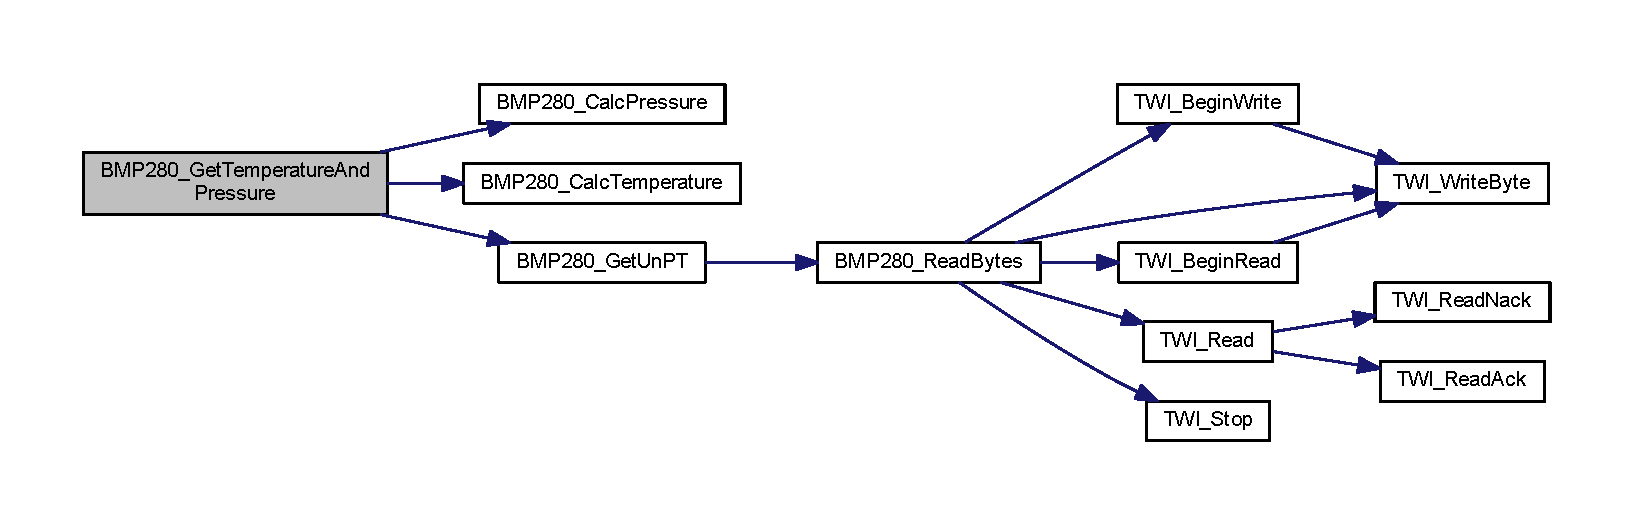
\includegraphics[width=350pt]{_b_m_p280_8h_aab0220cf4e61916eedbc1d5f72495c86_cgraph}
\end{center}
\end{figure}




Here is the caller graph for this function\-:
\nopagebreak
\begin{figure}[H]
\begin{center}
\leavevmode
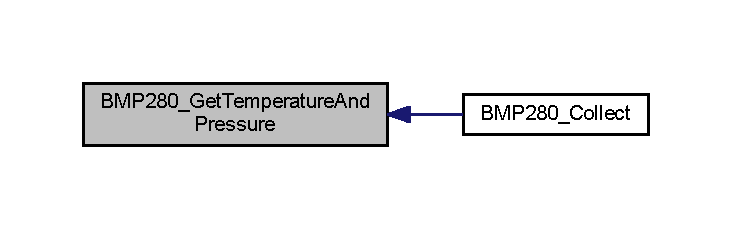
\includegraphics[width=350pt]{_b_m_p280_8h_aab0220cf4e61916eedbc1d5f72495c86_icgraph}
\end{center}
\end{figure}


\hypertarget{_b_m_p280_8h_a3aeeb100ef682ba3a48ea93ac87df141}{\index{B\-M\-P280.\-h@{B\-M\-P280.\-h}!B\-M\-P280\-\_\-\-Get\-Un\-P\-T@{B\-M\-P280\-\_\-\-Get\-Un\-P\-T}}
\index{B\-M\-P280\-\_\-\-Get\-Un\-P\-T@{B\-M\-P280\-\_\-\-Get\-Un\-P\-T}!BMP280.h@{B\-M\-P280.\-h}}
\subsubsection[{B\-M\-P280\-\_\-\-Get\-Un\-P\-T}]{\setlength{\rightskip}{0pt plus 5cm}char B\-M\-P280\-\_\-\-Get\-Un\-P\-T (
\begin{DoxyParamCaption}
\item[{double $\ast$}]{u\-P, }
\item[{double $\ast$}]{u\-T}
\end{DoxyParamCaption}
)}}\label{_b_m_p280_8h_a3aeeb100ef682ba3a48ea93ac87df141}


Gets the uncalibrated temperature and pressure data. 


\begin{DoxyParams}[1]{Parameters}
\mbox{\tt out}  & {\em pointer} & to a place to store the pressure data \\
\hline
\mbox{\tt out}  & {\em pointer} & to a place to store the temperature data \\
\hline
\end{DoxyParams}
\begin{DoxyReturn}{Returns}
status 
\end{DoxyReturn}


References B\-M\-P280\-\_\-\-Read\-Bytes(), and B\-M\-P280\-\_\-\-R\-E\-G\-\_\-\-R\-E\-S\-U\-L\-T\-\_\-\-P\-R\-E\-S\-S\-U\-R\-E.



Referenced by B\-M\-P280\-\_\-\-Get\-Temperature\-And\-Pressure().



Here is the call graph for this function\-:
\nopagebreak
\begin{figure}[H]
\begin{center}
\leavevmode
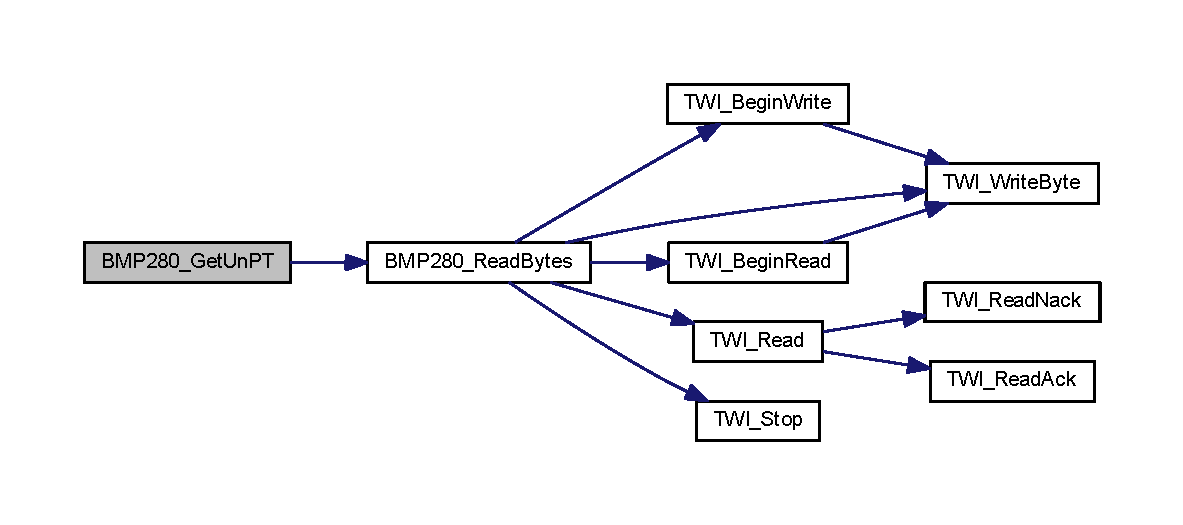
\includegraphics[width=350pt]{_b_m_p280_8h_a3aeeb100ef682ba3a48ea93ac87df141_cgraph}
\end{center}
\end{figure}




Here is the caller graph for this function\-:
\nopagebreak
\begin{figure}[H]
\begin{center}
\leavevmode
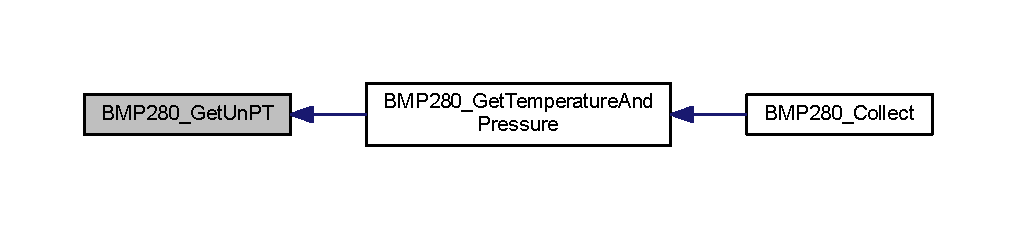
\includegraphics[width=350pt]{_b_m_p280_8h_a3aeeb100ef682ba3a48ea93ac87df141_icgraph}
\end{center}
\end{figure}


\hypertarget{_b_m_p280_8h_a2d512d05a3f329da6e0bfb081a1f6685}{\index{B\-M\-P280.\-h@{B\-M\-P280.\-h}!B\-M\-P280\-\_\-\-Init@{B\-M\-P280\-\_\-\-Init}}
\index{B\-M\-P280\-\_\-\-Init@{B\-M\-P280\-\_\-\-Init}!BMP280.h@{B\-M\-P280.\-h}}
\subsubsection[{B\-M\-P280\-\_\-\-Init}]{\setlength{\rightskip}{0pt plus 5cm}char B\-M\-P280\-\_\-\-Init (
\begin{DoxyParamCaption}
\item[{void}]{}
\end{DoxyParamCaption}
)}}\label{_b_m_p280_8h_a2d512d05a3f329da6e0bfb081a1f6685}


Initializes the B\-M\-P280 and reads the calibration data from the device. 

\begin{DoxyReturn}{Returns}
status (zero on failure, nonzero otherwise) 
\end{DoxyReturn}


References B\-M\-P280\-\_\-\-Read\-Int(), B\-M\-P280\-\_\-\-Read\-U\-Int(), dig\-\_\-\-P1, dig\-\_\-\-P2, dig\-\_\-\-P3, dig\-\_\-\-P4, dig\-\_\-\-P5, dig\-\_\-\-P6, dig\-\_\-\-P7, dig\-\_\-\-P8, dig\-\_\-\-P9, dig\-\_\-\-T1, dig\-\_\-\-T2, and dig\-\_\-\-T3.



Referenced by A\-P\-P\-\_\-\-Init().



Here is the call graph for this function\-:
\nopagebreak
\begin{figure}[H]
\begin{center}
\leavevmode
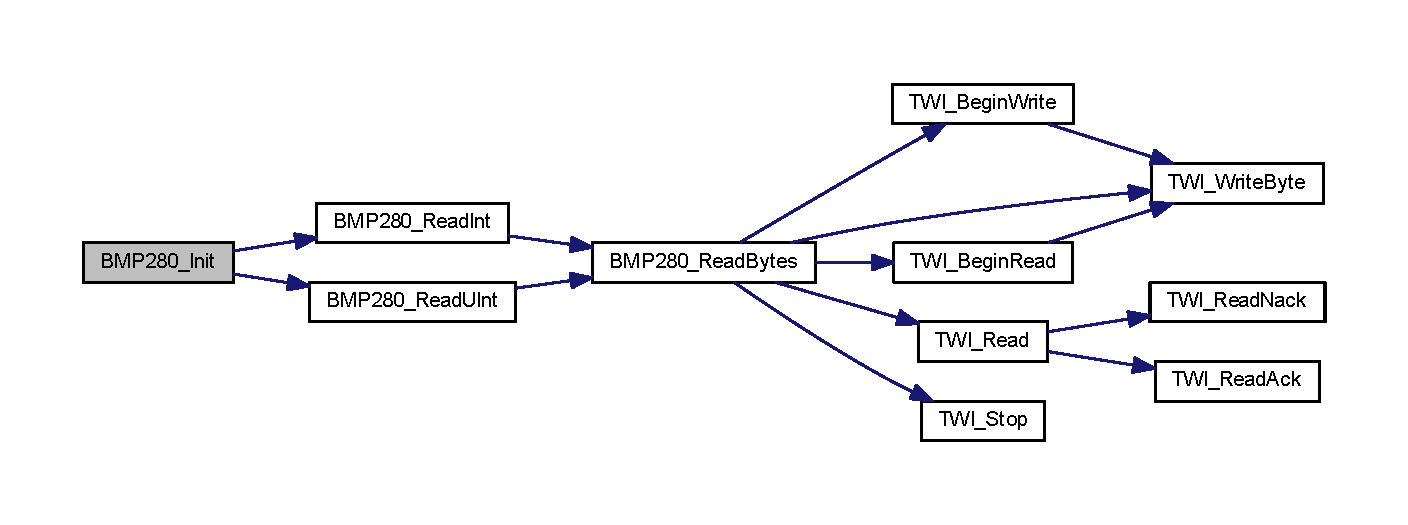
\includegraphics[width=350pt]{_b_m_p280_8h_a2d512d05a3f329da6e0bfb081a1f6685_cgraph}
\end{center}
\end{figure}




Here is the caller graph for this function\-:
\nopagebreak
\begin{figure}[H]
\begin{center}
\leavevmode
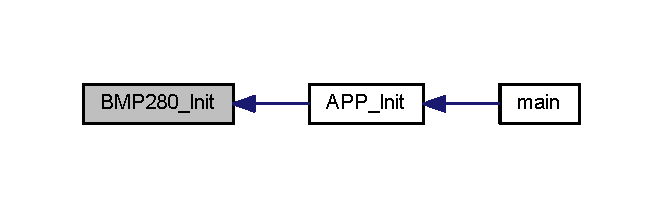
\includegraphics[width=318pt]{_b_m_p280_8h_a2d512d05a3f329da6e0bfb081a1f6685_icgraph}
\end{center}
\end{figure}


\hypertarget{_b_m_p280_8h_acfd338e24de5158c7ec8389d6c4eaa6a}{\index{B\-M\-P280.\-h@{B\-M\-P280.\-h}!B\-M\-P280\-\_\-\-Sealevel@{B\-M\-P280\-\_\-\-Sealevel}}
\index{B\-M\-P280\-\_\-\-Sealevel@{B\-M\-P280\-\_\-\-Sealevel}!BMP280.h@{B\-M\-P280.\-h}}
\subsubsection[{B\-M\-P280\-\_\-\-Sealevel}]{\setlength{\rightskip}{0pt plus 5cm}double B\-M\-P280\-\_\-\-Sealevel (
\begin{DoxyParamCaption}
\item[{double}]{P, }
\item[{double}]{A}
\end{DoxyParamCaption}
)}}\label{_b_m_p280_8h_acfd338e24de5158c7ec8389d6c4eaa6a}


Calculates pressure at sea level given an altitude. 


\begin{DoxyParams}[1]{Parameters}
\mbox{\tt in}  & {\em pressure} & reading \\
\hline
\mbox{\tt in}  & {\em altitude} & \\
\hline
\end{DoxyParams}
\begin{DoxyReturn}{Returns}
the corrected reading 
\end{DoxyReturn}
\hypertarget{_b_m_p280_8h_ac56b30a97fa1388153530bb658a0ab3d}{\index{B\-M\-P280.\-h@{B\-M\-P280.\-h}!B\-M\-P280\-\_\-\-Set\-Oversampling@{B\-M\-P280\-\_\-\-Set\-Oversampling}}
\index{B\-M\-P280\-\_\-\-Set\-Oversampling@{B\-M\-P280\-\_\-\-Set\-Oversampling}!BMP280.h@{B\-M\-P280.\-h}}
\subsubsection[{B\-M\-P280\-\_\-\-Set\-Oversampling}]{\setlength{\rightskip}{0pt plus 5cm}char B\-M\-P280\-\_\-\-Set\-Oversampling (
\begin{DoxyParamCaption}
\item[{short}]{oss}
\end{DoxyParamCaption}
)}}\label{_b_m_p280_8h_ac56b30a97fa1388153530bb658a0ab3d}


Sets the oversampling setting for the library. 


\begin{DoxyParams}[1]{Parameters}
\mbox{\tt in}  & {\em oss} & Oversampling setting \\
\hline
\end{DoxyParams}
\begin{DoxyReturn}{Returns}
1 
\end{DoxyReturn}


References oversampling.



Referenced by A\-P\-P\-\_\-\-Init().



Here is the caller graph for this function\-:
\nopagebreak
\begin{figure}[H]
\begin{center}
\leavevmode
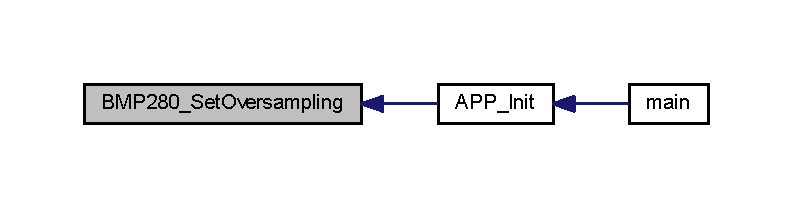
\includegraphics[width=350pt]{_b_m_p280_8h_ac56b30a97fa1388153530bb658a0ab3d_icgraph}
\end{center}
\end{figure}


\hypertarget{_b_m_p280_8h_a79fe54e0ce75dc946a3540bddd43e878}{\index{B\-M\-P280.\-h@{B\-M\-P280.\-h}!B\-M\-P280\-\_\-\-Start\-Measurment@{B\-M\-P280\-\_\-\-Start\-Measurment}}
\index{B\-M\-P280\-\_\-\-Start\-Measurment@{B\-M\-P280\-\_\-\-Start\-Measurment}!BMP280.h@{B\-M\-P280.\-h}}
\subsubsection[{B\-M\-P280\-\_\-\-Start\-Measurment}]{\setlength{\rightskip}{0pt plus 5cm}char B\-M\-P280\-\_\-\-Start\-Measurment (
\begin{DoxyParamCaption}
\item[{void}]{}
\end{DoxyParamCaption}
)}}\label{_b_m_p280_8h_a79fe54e0ce75dc946a3540bddd43e878}


Starts a measurement. 

\begin{DoxyReturn}{Returns}
time to wait for result (in ms) 
\end{DoxyReturn}


References B\-M\-P280\-\_\-\-C\-O\-M\-M\-A\-N\-D\-\_\-\-P\-R\-E\-S\-S\-U\-R\-E0, B\-M\-P280\-\_\-\-C\-O\-M\-M\-A\-N\-D\-\_\-\-P\-R\-E\-S\-S\-U\-R\-E1, B\-M\-P280\-\_\-\-C\-O\-M\-M\-A\-N\-D\-\_\-\-P\-R\-E\-S\-S\-U\-R\-E2, B\-M\-P280\-\_\-\-C\-O\-M\-M\-A\-N\-D\-\_\-\-P\-R\-E\-S\-S\-U\-R\-E3, B\-M\-P280\-\_\-\-C\-O\-M\-M\-A\-N\-D\-\_\-\-P\-R\-E\-S\-S\-U\-R\-E4, B\-M\-P280\-\_\-\-R\-E\-G\-\_\-\-C\-O\-N\-T\-R\-O\-L, B\-M\-P280\-\_\-\-Write\-Bytes(), delay, oversampling, and oversampling\-\_\-t.



Referenced by B\-M\-P280\-\_\-\-Request().



Here is the call graph for this function\-:
\nopagebreak
\begin{figure}[H]
\begin{center}
\leavevmode
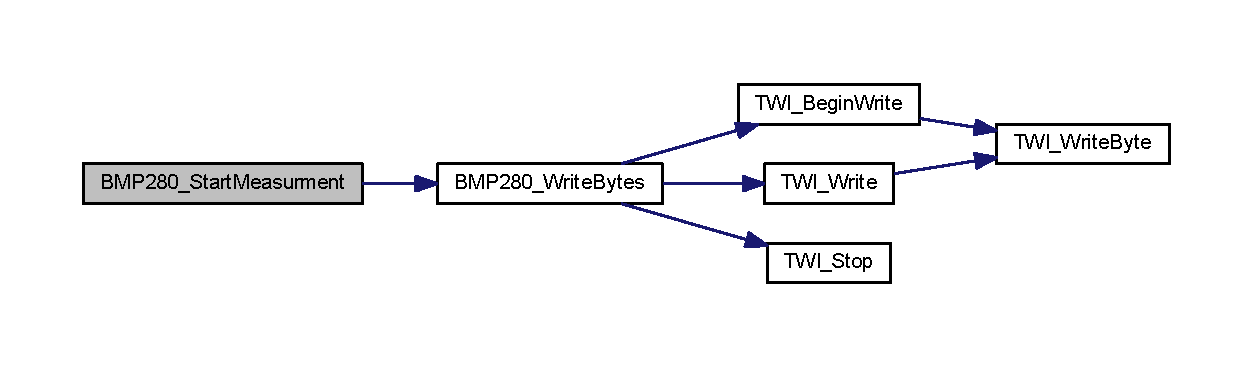
\includegraphics[width=350pt]{_b_m_p280_8h_a79fe54e0ce75dc946a3540bddd43e878_cgraph}
\end{center}
\end{figure}




Here is the caller graph for this function\-:
\nopagebreak
\begin{figure}[H]
\begin{center}
\leavevmode
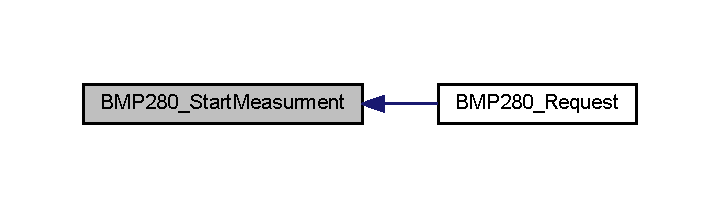
\includegraphics[width=346pt]{_b_m_p280_8h_a79fe54e0ce75dc946a3540bddd43e878_icgraph}
\end{center}
\end{figure}



\hypertarget{_k30_8h}{\section{C\-:/\-Users/\-A\-B/\-Documents/\-Git\-Hub/\-A\-T\-M\-E\-L-\/\-A\-T\-M\-O\-S/\-A\-T\-M\-O\-S/devices/inc/\-K30.h File Reference}
\label{_k30_8h}\index{C\-:/\-Users/\-A\-B/\-Documents/\-Git\-Hub/\-A\-T\-M\-E\-L-\/\-A\-T\-M\-O\-S/\-A\-T\-M\-O\-S/devices/inc/\-K30.\-h@{C\-:/\-Users/\-A\-B/\-Documents/\-Git\-Hub/\-A\-T\-M\-E\-L-\/\-A\-T\-M\-O\-S/\-A\-T\-M\-O\-S/devices/inc/\-K30.\-h}}
}


K30 Interface Library.  


{\ttfamily \#include $<$stdint.\-h$>$}\\*
Include dependency graph for K30.\-h\-:
\nopagebreak
\begin{figure}[H]
\begin{center}
\leavevmode
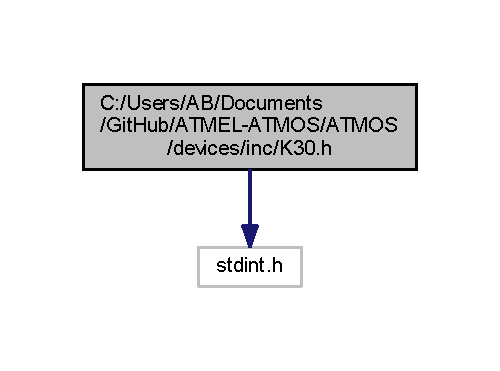
\includegraphics[width=240pt]{_k30_8h__incl}
\end{center}
\end{figure}
This graph shows which files directly or indirectly include this file\-:
\nopagebreak
\begin{figure}[H]
\begin{center}
\leavevmode
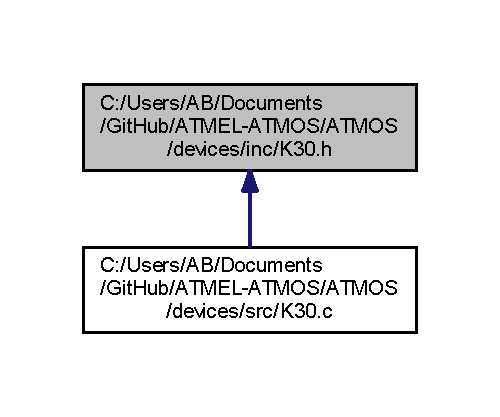
\includegraphics[width=240pt]{_k30_8h__dep__incl}
\end{center}
\end{figure}
\subsection*{Macros}
\begin{DoxyCompactItemize}
\item 
\#define \hyperlink{_k30_8h_aaaaa703bb9584ab862010529ed057109}{K30\-\_\-\-A\-D\-D\-R}~0x68
\item 
\#define \hyperlink{_k30_8h_a11fca5e6f68f58d01887d2a0d360c29e}{K30\-\_\-\-I2\-\_\-\-R\-A\-M\-\_\-\-A\-D\-D\-R}~0x20
\item 
\#define \hyperlink{_k30_8h_aa725aa6c183705b6da3aea0f54184ab1}{K30\-\_\-\-I2\-\_\-\-E\-E\-P\-R\-O\-M\-\_\-\-A\-D\-D\-R}~0x00
\item 
\#define \hyperlink{_k30_8h_a6ed1b7ebcf9a7bf84979813a65a6611e}{S\-H\-I\-F\-T\-E\-D\-\_\-\-D\-I\-V\-I\-S\-O\-R}~0x988000
\item 
\#define \hyperlink{_k30_8h_a13b8270fa09cc3781a2b1b24ca949790}{K30\-\_\-\-W\-R\-I\-T\-E}~0x\-D0
\item 
\#define \hyperlink{_k30_8h_a768c5bc61c56d18904e62d5fe935f832}{K30\-\_\-\-R\-E\-A\-D\-\_\-\-R\-A\-M}~0x22
\item 
\#define \hyperlink{_k30_8h_aa1e70f14664cbab89a0035e77e726d9d}{K30\-\_\-\-R\-A\-M\-\_\-\-H\-I\-\_\-\-B\-Y\-T\-E}~0x08
\item 
\#define \hyperlink{_k30_8h_a5dfb4316839124a623b0f906717061bf}{K30\-\_\-\-R\-A\-M\-\_\-\-L\-O\-\_\-\-B\-Y\-T\-E}~0x09
\end{DoxyCompactItemize}
\subsection*{Functions}
\begin{DoxyCompactItemize}
\item 
int \hyperlink{_k30_8h_a9749b047bc23704623901452834f78b5}{K30\-\_\-read\-C\-O2} ()
\begin{DoxyCompactList}\small\item\em Initializes the K30. \end{DoxyCompactList}\end{DoxyCompactItemize}


\subsection{Detailed Description}
K30 Interface Library. Created\-: 04/02/2015 18\-:04\-:55 Author\-: Hui Shi 

\subsection{Macro Definition Documentation}
\hypertarget{_k30_8h_aaaaa703bb9584ab862010529ed057109}{\index{K30.\-h@{K30.\-h}!K30\-\_\-\-A\-D\-D\-R@{K30\-\_\-\-A\-D\-D\-R}}
\index{K30\-\_\-\-A\-D\-D\-R@{K30\-\_\-\-A\-D\-D\-R}!K30.h@{K30.\-h}}
\subsubsection[{K30\-\_\-\-A\-D\-D\-R}]{\setlength{\rightskip}{0pt plus 5cm}\#define K30\-\_\-\-A\-D\-D\-R~0x68}}\label{_k30_8h_aaaaa703bb9584ab862010529ed057109}
\hypertarget{_k30_8h_aa725aa6c183705b6da3aea0f54184ab1}{\index{K30.\-h@{K30.\-h}!K30\-\_\-\-I2\-\_\-\-E\-E\-P\-R\-O\-M\-\_\-\-A\-D\-D\-R@{K30\-\_\-\-I2\-\_\-\-E\-E\-P\-R\-O\-M\-\_\-\-A\-D\-D\-R}}
\index{K30\-\_\-\-I2\-\_\-\-E\-E\-P\-R\-O\-M\-\_\-\-A\-D\-D\-R@{K30\-\_\-\-I2\-\_\-\-E\-E\-P\-R\-O\-M\-\_\-\-A\-D\-D\-R}!K30.h@{K30.\-h}}
\subsubsection[{K30\-\_\-\-I2\-\_\-\-E\-E\-P\-R\-O\-M\-\_\-\-A\-D\-D\-R}]{\setlength{\rightskip}{0pt plus 5cm}\#define K30\-\_\-\-I2\-\_\-\-E\-E\-P\-R\-O\-M\-\_\-\-A\-D\-D\-R~0x00}}\label{_k30_8h_aa725aa6c183705b6da3aea0f54184ab1}
\hypertarget{_k30_8h_a11fca5e6f68f58d01887d2a0d360c29e}{\index{K30.\-h@{K30.\-h}!K30\-\_\-\-I2\-\_\-\-R\-A\-M\-\_\-\-A\-D\-D\-R@{K30\-\_\-\-I2\-\_\-\-R\-A\-M\-\_\-\-A\-D\-D\-R}}
\index{K30\-\_\-\-I2\-\_\-\-R\-A\-M\-\_\-\-A\-D\-D\-R@{K30\-\_\-\-I2\-\_\-\-R\-A\-M\-\_\-\-A\-D\-D\-R}!K30.h@{K30.\-h}}
\subsubsection[{K30\-\_\-\-I2\-\_\-\-R\-A\-M\-\_\-\-A\-D\-D\-R}]{\setlength{\rightskip}{0pt plus 5cm}\#define K30\-\_\-\-I2\-\_\-\-R\-A\-M\-\_\-\-A\-D\-D\-R~0x20}}\label{_k30_8h_a11fca5e6f68f58d01887d2a0d360c29e}
\hypertarget{_k30_8h_aa1e70f14664cbab89a0035e77e726d9d}{\index{K30.\-h@{K30.\-h}!K30\-\_\-\-R\-A\-M\-\_\-\-H\-I\-\_\-\-B\-Y\-T\-E@{K30\-\_\-\-R\-A\-M\-\_\-\-H\-I\-\_\-\-B\-Y\-T\-E}}
\index{K30\-\_\-\-R\-A\-M\-\_\-\-H\-I\-\_\-\-B\-Y\-T\-E@{K30\-\_\-\-R\-A\-M\-\_\-\-H\-I\-\_\-\-B\-Y\-T\-E}!K30.h@{K30.\-h}}
\subsubsection[{K30\-\_\-\-R\-A\-M\-\_\-\-H\-I\-\_\-\-B\-Y\-T\-E}]{\setlength{\rightskip}{0pt plus 5cm}\#define K30\-\_\-\-R\-A\-M\-\_\-\-H\-I\-\_\-\-B\-Y\-T\-E~0x08}}\label{_k30_8h_aa1e70f14664cbab89a0035e77e726d9d}
\hypertarget{_k30_8h_a5dfb4316839124a623b0f906717061bf}{\index{K30.\-h@{K30.\-h}!K30\-\_\-\-R\-A\-M\-\_\-\-L\-O\-\_\-\-B\-Y\-T\-E@{K30\-\_\-\-R\-A\-M\-\_\-\-L\-O\-\_\-\-B\-Y\-T\-E}}
\index{K30\-\_\-\-R\-A\-M\-\_\-\-L\-O\-\_\-\-B\-Y\-T\-E@{K30\-\_\-\-R\-A\-M\-\_\-\-L\-O\-\_\-\-B\-Y\-T\-E}!K30.h@{K30.\-h}}
\subsubsection[{K30\-\_\-\-R\-A\-M\-\_\-\-L\-O\-\_\-\-B\-Y\-T\-E}]{\setlength{\rightskip}{0pt plus 5cm}\#define K30\-\_\-\-R\-A\-M\-\_\-\-L\-O\-\_\-\-B\-Y\-T\-E~0x09}}\label{_k30_8h_a5dfb4316839124a623b0f906717061bf}
\hypertarget{_k30_8h_a768c5bc61c56d18904e62d5fe935f832}{\index{K30.\-h@{K30.\-h}!K30\-\_\-\-R\-E\-A\-D\-\_\-\-R\-A\-M@{K30\-\_\-\-R\-E\-A\-D\-\_\-\-R\-A\-M}}
\index{K30\-\_\-\-R\-E\-A\-D\-\_\-\-R\-A\-M@{K30\-\_\-\-R\-E\-A\-D\-\_\-\-R\-A\-M}!K30.h@{K30.\-h}}
\subsubsection[{K30\-\_\-\-R\-E\-A\-D\-\_\-\-R\-A\-M}]{\setlength{\rightskip}{0pt plus 5cm}\#define K30\-\_\-\-R\-E\-A\-D\-\_\-\-R\-A\-M~0x22}}\label{_k30_8h_a768c5bc61c56d18904e62d5fe935f832}
\hypertarget{_k30_8h_a13b8270fa09cc3781a2b1b24ca949790}{\index{K30.\-h@{K30.\-h}!K30\-\_\-\-W\-R\-I\-T\-E@{K30\-\_\-\-W\-R\-I\-T\-E}}
\index{K30\-\_\-\-W\-R\-I\-T\-E@{K30\-\_\-\-W\-R\-I\-T\-E}!K30.h@{K30.\-h}}
\subsubsection[{K30\-\_\-\-W\-R\-I\-T\-E}]{\setlength{\rightskip}{0pt plus 5cm}\#define K30\-\_\-\-W\-R\-I\-T\-E~0x\-D0}}\label{_k30_8h_a13b8270fa09cc3781a2b1b24ca949790}
Status Codes \hypertarget{_k30_8h_a6ed1b7ebcf9a7bf84979813a65a6611e}{\index{K30.\-h@{K30.\-h}!S\-H\-I\-F\-T\-E\-D\-\_\-\-D\-I\-V\-I\-S\-O\-R@{S\-H\-I\-F\-T\-E\-D\-\_\-\-D\-I\-V\-I\-S\-O\-R}}
\index{S\-H\-I\-F\-T\-E\-D\-\_\-\-D\-I\-V\-I\-S\-O\-R@{S\-H\-I\-F\-T\-E\-D\-\_\-\-D\-I\-V\-I\-S\-O\-R}!K30.h@{K30.\-h}}
\subsubsection[{S\-H\-I\-F\-T\-E\-D\-\_\-\-D\-I\-V\-I\-S\-O\-R}]{\setlength{\rightskip}{0pt plus 5cm}\#define S\-H\-I\-F\-T\-E\-D\-\_\-\-D\-I\-V\-I\-S\-O\-R~0x988000}}\label{_k30_8h_a6ed1b7ebcf9a7bf84979813a65a6611e}


Referenced by check\-\_\-crc().



\subsection{Function Documentation}
\hypertarget{_k30_8h_a9749b047bc23704623901452834f78b5}{\index{K30.\-h@{K30.\-h}!K30\-\_\-read\-C\-O2@{K30\-\_\-read\-C\-O2}}
\index{K30\-\_\-read\-C\-O2@{K30\-\_\-read\-C\-O2}!K30.h@{K30.\-h}}
\subsubsection[{K30\-\_\-read\-C\-O2}]{\setlength{\rightskip}{0pt plus 5cm}int K30\-\_\-read\-C\-O2 (
\begin{DoxyParamCaption}
{}
\end{DoxyParamCaption}
)}}\label{_k30_8h_a9749b047bc23704623901452834f78b5}


Initializes the K30. 

\begin{DoxyReturn}{Returns}
status zero 
\end{DoxyReturn}


References buffer, readcmd, status, T\-W\-I\-\_\-\-Begin\-Read(), T\-W\-I\-\_\-\-Begin\-Write(), T\-W\-I\-\_\-\-Read(), T\-W\-I\-\_\-\-R\-E\-C\-\_\-\-A\-C\-K, T\-W\-I\-\_\-\-S\-E\-N\-T\-\_\-\-A\-C\-K, T\-W\-I\-\_\-\-S\-L\-A\-R\-\_\-\-A\-C\-K, T\-W\-I\-\_\-\-S\-L\-A\-W\-\_\-\-A\-C\-K, T\-W\-I\-\_\-\-Stop(), and T\-W\-I\-\_\-\-Write().



Here is the call graph for this function\-:
\nopagebreak
\begin{figure}[H]
\begin{center}
\leavevmode
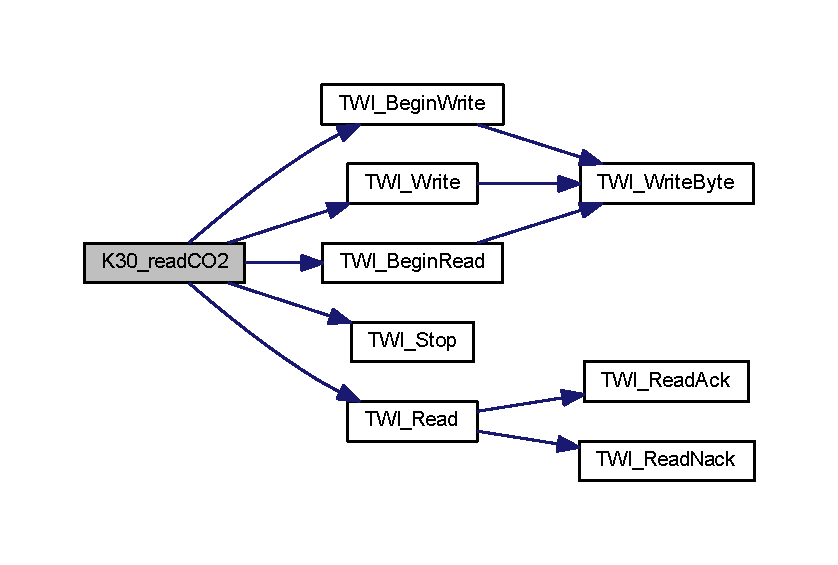
\includegraphics[width=350pt]{_k30_8h_a9749b047bc23704623901452834f78b5_cgraph}
\end{center}
\end{figure}



\hypertarget{_si7020_8h}{\section{C\-:/\-Users/\-A\-B/\-Documents/\-Git\-Hub/\-A\-T\-M\-E\-L-\/\-A\-T\-M\-O\-S/\-A\-T\-M\-O\-S/devices/inc/\-Si7020.h File Reference}
\label{_si7020_8h}\index{C\-:/\-Users/\-A\-B/\-Documents/\-Git\-Hub/\-A\-T\-M\-E\-L-\/\-A\-T\-M\-O\-S/\-A\-T\-M\-O\-S/devices/inc/\-Si7020.\-h@{C\-:/\-Users/\-A\-B/\-Documents/\-Git\-Hub/\-A\-T\-M\-E\-L-\/\-A\-T\-M\-O\-S/\-A\-T\-M\-O\-S/devices/inc/\-Si7020.\-h}}
}


Si7020 Interface Library.  


{\ttfamily \#include $<$stdint.\-h$>$}\\*
Include dependency graph for Si7020.\-h\-:
\nopagebreak
\begin{figure}[H]
\begin{center}
\leavevmode
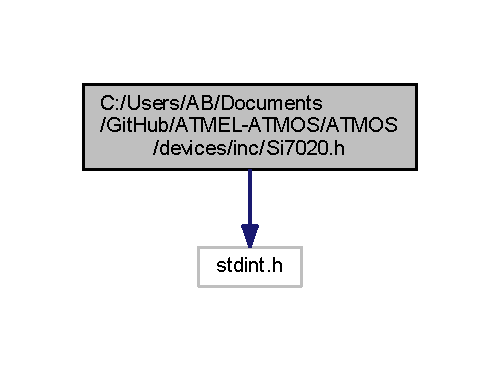
\includegraphics[width=240pt]{_si7020_8h__incl}
\end{center}
\end{figure}
This graph shows which files directly or indirectly include this file\-:
\nopagebreak
\begin{figure}[H]
\begin{center}
\leavevmode
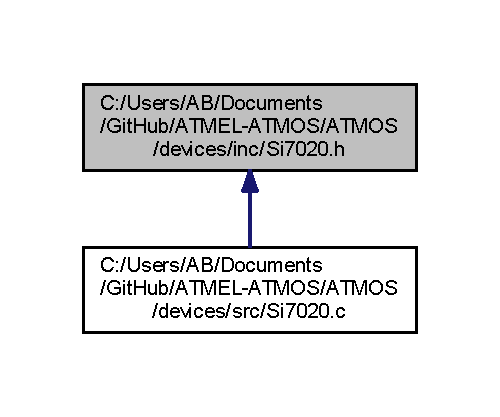
\includegraphics[width=240pt]{_si7020_8h__dep__incl}
\end{center}
\end{figure}
\subsection*{Macros}
\begin{DoxyCompactItemize}
\item 
\#define \hyperlink{_si7020_8h_afff2812ca001e5c56254a301dbede825}{S\-I7020\-\_\-\-A\-D\-D\-R}~0x40
\item 
\#define \hyperlink{_si7020_8h_ad8588e4f0a0464884899f27ece06ae67}{S\-I7020\-\_\-\-R\-E\-L\-\_\-\-H\-U\-M\-I\-D\-I\-T\-Y\-\_\-\-H\-O\-L\-D}~0x\-E5
\item 
\#define \hyperlink{_si7020_8h_a84b62936cb987c0c57473bcf806ef5cc}{S\-I7020\-\_\-\-R\-E\-L\-\_\-\-H\-U\-M\-I\-D\-I\-T\-Y\-\_\-\-N\-O\-N\-H\-O\-L\-D}~0x\-F5
\item 
\#define \hyperlink{_si7020_8h_a87bc2a9a6f3c12f880a803cbe758e0ae}{S\-I7020\-\_\-\-T\-E\-M\-P\-E\-R\-A\-T\-U\-R\-E\-\_\-\-H\-O\-L\-D}~0x\-E3
\item 
\#define \hyperlink{_si7020_8h_a30ecc68510a209cd3c7f8df33e565a6f}{S\-I7020\-\_\-\-T\-E\-M\-P\-E\-R\-A\-T\-U\-R\-E\-\_\-\-N\-O\-H\-O\-L\-D}~0x\-F3
\item 
\#define \hyperlink{_si7020_8h_a932d4b9499d7a05d70f917d66771f3b7}{S\-I7020\-\_\-\-R\-D\-\_\-\-T\-E\-M\-P\-\_\-\-P\-R\-E\-\_\-\-R\-H}~0x\-E0
\item 
\#define \hyperlink{_si7020_8h_adba36e4cc4f209030231eadb1f3a90fe}{S\-I7020\-\_\-\-R\-E\-S\-E\-T}~0x\-F\-E
\item 
\#define \hyperlink{_si7020_8h_a9dbe1feadc8758d190bcea84ae991e2b}{S\-I7020\-\_\-\-W\-R\-\_\-\-R\-H\-\_\-\-T\-\_\-\-R\-E\-G1}~0x\-E6
\item 
\#define \hyperlink{_si7020_8h_a51403c4e1be19e16733a3e49594fc6fb}{S\-I7020\-\_\-\-R\-D\-\_\-\-R\-H\-\_\-\-T\-\_\-\-R\-E\-G1}~0x\-E7
\item 
\#define \hyperlink{_si7020_8h_a6e8822306ba989c166f6bdfce007654d}{S\-I7020\-\_\-\-W\-R\-\_\-\-H\-E\-A\-T\-\_\-\-C\-T\-R\-\_\-\-R\-E\-G}~0x51
\item 
\#define \hyperlink{_si7020_8h_afcf7b09858c8c8b354aab4a6f523ab47}{S\-I7020\-\_\-\-R\-D\-\_\-\-H\-E\-A\-T\-\_\-\-C\-T\-R\-\_\-\-R\-E\-G}~0x11
\item 
\#define \hyperlink{_si7020_8h_a281481f3083c7e10edd8cbb14f1b00d5}{S\-I7020\-\_\-\-E\-L\-C\-I\-D\-\_\-1\-S\-T\-\_\-\-B\-Y\-T\-E}~0x\-F\-A
\item 
\#define \hyperlink{_si7020_8h_ab9a61c841eb8cfb4b4a0dfc787637888}{S\-I7020\-\_\-\-E\-L\-C\-I\-D\-\_\-2\-N\-D\-\_\-\-B\-Y\-T\-E}~0x\-F\-C
\item 
\#define \hyperlink{_si7020_8h_a02a48291f7605a9e2164b18d20bf86ef}{S\-I7020\-\_\-\-F\-I\-R\-M\-W\-A\-R\-E\-\_\-\-R\-E\-V}~0x84
\item 
\#define \hyperlink{_si7020_8h_a6ed1b7ebcf9a7bf84979813a65a6611e}{S\-H\-I\-F\-T\-E\-D\-\_\-\-D\-I\-V\-I\-S\-O\-R}~0x988000
\end{DoxyCompactItemize}
\subsection*{Functions}
\begin{DoxyCompactItemize}
\item 
char \hyperlink{_si7020_8h_a75e9271e7a15c900a748e79f01d3c5be}{Si7020\-\_\-init} ()
\begin{DoxyCompactList}\small\item\em Initializes the Si7020. \end{DoxyCompactList}\item 
char \hyperlink{_si7020_8h_aebde99dd234f560632ecdbe126b67e05}{Si7020\-\_\-read\-Humidity} (unsigned char $\ast$, char)
\begin{DoxyCompactList}\small\item\em Read humidity from Si7020. \end{DoxyCompactList}\item 
char \hyperlink{_si7020_8h_ac561f9976fbf8f27a921f55fc402548d}{Si7020\-\_\-read\-Temperature} (unsigned char $\ast$, char)
\begin{DoxyCompactList}\small\item\em Read temperature from Si7020. \end{DoxyCompactList}\item 
float \hyperlink{_si7020_8h_afa24936aee0e87d37acc2ed57286c28a}{Si7020\-\_\-cal\-Humidity} (unsigned char $\ast$)
\begin{DoxyCompactList}\small\item\em Calculate humidity from Si7020. \end{DoxyCompactList}\item 
float \hyperlink{_si7020_8h_ab74020292e05d0f98013df991f6c4568}{Si7020\-\_\-cal\-Temperature} (unsigned char $\ast$)
\begin{DoxyCompactList}\small\item\em Calculate temperature from Si7020. \end{DoxyCompactList}\end{DoxyCompactItemize}


\subsection{Detailed Description}
Si7020 Interface Library. Created\-: 3/27/2015 11\-:14\-:55 Author\-: Hui Shi 

\subsection{Macro Definition Documentation}
\hypertarget{_si7020_8h_a6ed1b7ebcf9a7bf84979813a65a6611e}{\index{Si7020.\-h@{Si7020.\-h}!S\-H\-I\-F\-T\-E\-D\-\_\-\-D\-I\-V\-I\-S\-O\-R@{S\-H\-I\-F\-T\-E\-D\-\_\-\-D\-I\-V\-I\-S\-O\-R}}
\index{S\-H\-I\-F\-T\-E\-D\-\_\-\-D\-I\-V\-I\-S\-O\-R@{S\-H\-I\-F\-T\-E\-D\-\_\-\-D\-I\-V\-I\-S\-O\-R}!Si7020.h@{Si7020.\-h}}
\subsubsection[{S\-H\-I\-F\-T\-E\-D\-\_\-\-D\-I\-V\-I\-S\-O\-R}]{\setlength{\rightskip}{0pt plus 5cm}\#define S\-H\-I\-F\-T\-E\-D\-\_\-\-D\-I\-V\-I\-S\-O\-R~0x988000}}\label{_si7020_8h_a6ed1b7ebcf9a7bf84979813a65a6611e}
\hypertarget{_si7020_8h_afff2812ca001e5c56254a301dbede825}{\index{Si7020.\-h@{Si7020.\-h}!S\-I7020\-\_\-\-A\-D\-D\-R@{S\-I7020\-\_\-\-A\-D\-D\-R}}
\index{S\-I7020\-\_\-\-A\-D\-D\-R@{S\-I7020\-\_\-\-A\-D\-D\-R}!Si7020.h@{Si7020.\-h}}
\subsubsection[{S\-I7020\-\_\-\-A\-D\-D\-R}]{\setlength{\rightskip}{0pt plus 5cm}\#define S\-I7020\-\_\-\-A\-D\-D\-R~0x40}}\label{_si7020_8h_afff2812ca001e5c56254a301dbede825}


Referenced by Si7020\-\_\-read\-Humidity(), and Si7020\-\_\-read\-Temperature().

\hypertarget{_si7020_8h_a281481f3083c7e10edd8cbb14f1b00d5}{\index{Si7020.\-h@{Si7020.\-h}!S\-I7020\-\_\-\-E\-L\-C\-I\-D\-\_\-1\-S\-T\-\_\-\-B\-Y\-T\-E@{S\-I7020\-\_\-\-E\-L\-C\-I\-D\-\_\-1\-S\-T\-\_\-\-B\-Y\-T\-E}}
\index{S\-I7020\-\_\-\-E\-L\-C\-I\-D\-\_\-1\-S\-T\-\_\-\-B\-Y\-T\-E@{S\-I7020\-\_\-\-E\-L\-C\-I\-D\-\_\-1\-S\-T\-\_\-\-B\-Y\-T\-E}!Si7020.h@{Si7020.\-h}}
\subsubsection[{S\-I7020\-\_\-\-E\-L\-C\-I\-D\-\_\-1\-S\-T\-\_\-\-B\-Y\-T\-E}]{\setlength{\rightskip}{0pt plus 5cm}\#define S\-I7020\-\_\-\-E\-L\-C\-I\-D\-\_\-1\-S\-T\-\_\-\-B\-Y\-T\-E~0x\-F\-A}}\label{_si7020_8h_a281481f3083c7e10edd8cbb14f1b00d5}
\hypertarget{_si7020_8h_ab9a61c841eb8cfb4b4a0dfc787637888}{\index{Si7020.\-h@{Si7020.\-h}!S\-I7020\-\_\-\-E\-L\-C\-I\-D\-\_\-2\-N\-D\-\_\-\-B\-Y\-T\-E@{S\-I7020\-\_\-\-E\-L\-C\-I\-D\-\_\-2\-N\-D\-\_\-\-B\-Y\-T\-E}}
\index{S\-I7020\-\_\-\-E\-L\-C\-I\-D\-\_\-2\-N\-D\-\_\-\-B\-Y\-T\-E@{S\-I7020\-\_\-\-E\-L\-C\-I\-D\-\_\-2\-N\-D\-\_\-\-B\-Y\-T\-E}!Si7020.h@{Si7020.\-h}}
\subsubsection[{S\-I7020\-\_\-\-E\-L\-C\-I\-D\-\_\-2\-N\-D\-\_\-\-B\-Y\-T\-E}]{\setlength{\rightskip}{0pt plus 5cm}\#define S\-I7020\-\_\-\-E\-L\-C\-I\-D\-\_\-2\-N\-D\-\_\-\-B\-Y\-T\-E~0x\-F\-C}}\label{_si7020_8h_ab9a61c841eb8cfb4b4a0dfc787637888}
\hypertarget{_si7020_8h_a02a48291f7605a9e2164b18d20bf86ef}{\index{Si7020.\-h@{Si7020.\-h}!S\-I7020\-\_\-\-F\-I\-R\-M\-W\-A\-R\-E\-\_\-\-R\-E\-V@{S\-I7020\-\_\-\-F\-I\-R\-M\-W\-A\-R\-E\-\_\-\-R\-E\-V}}
\index{S\-I7020\-\_\-\-F\-I\-R\-M\-W\-A\-R\-E\-\_\-\-R\-E\-V@{S\-I7020\-\_\-\-F\-I\-R\-M\-W\-A\-R\-E\-\_\-\-R\-E\-V}!Si7020.h@{Si7020.\-h}}
\subsubsection[{S\-I7020\-\_\-\-F\-I\-R\-M\-W\-A\-R\-E\-\_\-\-R\-E\-V}]{\setlength{\rightskip}{0pt plus 5cm}\#define S\-I7020\-\_\-\-F\-I\-R\-M\-W\-A\-R\-E\-\_\-\-R\-E\-V~0x84}}\label{_si7020_8h_a02a48291f7605a9e2164b18d20bf86ef}
\hypertarget{_si7020_8h_afcf7b09858c8c8b354aab4a6f523ab47}{\index{Si7020.\-h@{Si7020.\-h}!S\-I7020\-\_\-\-R\-D\-\_\-\-H\-E\-A\-T\-\_\-\-C\-T\-R\-\_\-\-R\-E\-G@{S\-I7020\-\_\-\-R\-D\-\_\-\-H\-E\-A\-T\-\_\-\-C\-T\-R\-\_\-\-R\-E\-G}}
\index{S\-I7020\-\_\-\-R\-D\-\_\-\-H\-E\-A\-T\-\_\-\-C\-T\-R\-\_\-\-R\-E\-G@{S\-I7020\-\_\-\-R\-D\-\_\-\-H\-E\-A\-T\-\_\-\-C\-T\-R\-\_\-\-R\-E\-G}!Si7020.h@{Si7020.\-h}}
\subsubsection[{S\-I7020\-\_\-\-R\-D\-\_\-\-H\-E\-A\-T\-\_\-\-C\-T\-R\-\_\-\-R\-E\-G}]{\setlength{\rightskip}{0pt plus 5cm}\#define S\-I7020\-\_\-\-R\-D\-\_\-\-H\-E\-A\-T\-\_\-\-C\-T\-R\-\_\-\-R\-E\-G~0x11}}\label{_si7020_8h_afcf7b09858c8c8b354aab4a6f523ab47}
\hypertarget{_si7020_8h_a51403c4e1be19e16733a3e49594fc6fb}{\index{Si7020.\-h@{Si7020.\-h}!S\-I7020\-\_\-\-R\-D\-\_\-\-R\-H\-\_\-\-T\-\_\-\-R\-E\-G1@{S\-I7020\-\_\-\-R\-D\-\_\-\-R\-H\-\_\-\-T\-\_\-\-R\-E\-G1}}
\index{S\-I7020\-\_\-\-R\-D\-\_\-\-R\-H\-\_\-\-T\-\_\-\-R\-E\-G1@{S\-I7020\-\_\-\-R\-D\-\_\-\-R\-H\-\_\-\-T\-\_\-\-R\-E\-G1}!Si7020.h@{Si7020.\-h}}
\subsubsection[{S\-I7020\-\_\-\-R\-D\-\_\-\-R\-H\-\_\-\-T\-\_\-\-R\-E\-G1}]{\setlength{\rightskip}{0pt plus 5cm}\#define S\-I7020\-\_\-\-R\-D\-\_\-\-R\-H\-\_\-\-T\-\_\-\-R\-E\-G1~0x\-E7}}\label{_si7020_8h_a51403c4e1be19e16733a3e49594fc6fb}
\hypertarget{_si7020_8h_a932d4b9499d7a05d70f917d66771f3b7}{\index{Si7020.\-h@{Si7020.\-h}!S\-I7020\-\_\-\-R\-D\-\_\-\-T\-E\-M\-P\-\_\-\-P\-R\-E\-\_\-\-R\-H@{S\-I7020\-\_\-\-R\-D\-\_\-\-T\-E\-M\-P\-\_\-\-P\-R\-E\-\_\-\-R\-H}}
\index{S\-I7020\-\_\-\-R\-D\-\_\-\-T\-E\-M\-P\-\_\-\-P\-R\-E\-\_\-\-R\-H@{S\-I7020\-\_\-\-R\-D\-\_\-\-T\-E\-M\-P\-\_\-\-P\-R\-E\-\_\-\-R\-H}!Si7020.h@{Si7020.\-h}}
\subsubsection[{S\-I7020\-\_\-\-R\-D\-\_\-\-T\-E\-M\-P\-\_\-\-P\-R\-E\-\_\-\-R\-H}]{\setlength{\rightskip}{0pt plus 5cm}\#define S\-I7020\-\_\-\-R\-D\-\_\-\-T\-E\-M\-P\-\_\-\-P\-R\-E\-\_\-\-R\-H~0x\-E0}}\label{_si7020_8h_a932d4b9499d7a05d70f917d66771f3b7}
\hypertarget{_si7020_8h_ad8588e4f0a0464884899f27ece06ae67}{\index{Si7020.\-h@{Si7020.\-h}!S\-I7020\-\_\-\-R\-E\-L\-\_\-\-H\-U\-M\-I\-D\-I\-T\-Y\-\_\-\-H\-O\-L\-D@{S\-I7020\-\_\-\-R\-E\-L\-\_\-\-H\-U\-M\-I\-D\-I\-T\-Y\-\_\-\-H\-O\-L\-D}}
\index{S\-I7020\-\_\-\-R\-E\-L\-\_\-\-H\-U\-M\-I\-D\-I\-T\-Y\-\_\-\-H\-O\-L\-D@{S\-I7020\-\_\-\-R\-E\-L\-\_\-\-H\-U\-M\-I\-D\-I\-T\-Y\-\_\-\-H\-O\-L\-D}!Si7020.h@{Si7020.\-h}}
\subsubsection[{S\-I7020\-\_\-\-R\-E\-L\-\_\-\-H\-U\-M\-I\-D\-I\-T\-Y\-\_\-\-H\-O\-L\-D}]{\setlength{\rightskip}{0pt plus 5cm}\#define S\-I7020\-\_\-\-R\-E\-L\-\_\-\-H\-U\-M\-I\-D\-I\-T\-Y\-\_\-\-H\-O\-L\-D~0x\-E5}}\label{_si7020_8h_ad8588e4f0a0464884899f27ece06ae67}
Status Codes 

Referenced by Si7020\-\_\-read\-Humidity().

\hypertarget{_si7020_8h_a84b62936cb987c0c57473bcf806ef5cc}{\index{Si7020.\-h@{Si7020.\-h}!S\-I7020\-\_\-\-R\-E\-L\-\_\-\-H\-U\-M\-I\-D\-I\-T\-Y\-\_\-\-N\-O\-N\-H\-O\-L\-D@{S\-I7020\-\_\-\-R\-E\-L\-\_\-\-H\-U\-M\-I\-D\-I\-T\-Y\-\_\-\-N\-O\-N\-H\-O\-L\-D}}
\index{S\-I7020\-\_\-\-R\-E\-L\-\_\-\-H\-U\-M\-I\-D\-I\-T\-Y\-\_\-\-N\-O\-N\-H\-O\-L\-D@{S\-I7020\-\_\-\-R\-E\-L\-\_\-\-H\-U\-M\-I\-D\-I\-T\-Y\-\_\-\-N\-O\-N\-H\-O\-L\-D}!Si7020.h@{Si7020.\-h}}
\subsubsection[{S\-I7020\-\_\-\-R\-E\-L\-\_\-\-H\-U\-M\-I\-D\-I\-T\-Y\-\_\-\-N\-O\-N\-H\-O\-L\-D}]{\setlength{\rightskip}{0pt plus 5cm}\#define S\-I7020\-\_\-\-R\-E\-L\-\_\-\-H\-U\-M\-I\-D\-I\-T\-Y\-\_\-\-N\-O\-N\-H\-O\-L\-D~0x\-F5}}\label{_si7020_8h_a84b62936cb987c0c57473bcf806ef5cc}
\hypertarget{_si7020_8h_adba36e4cc4f209030231eadb1f3a90fe}{\index{Si7020.\-h@{Si7020.\-h}!S\-I7020\-\_\-\-R\-E\-S\-E\-T@{S\-I7020\-\_\-\-R\-E\-S\-E\-T}}
\index{S\-I7020\-\_\-\-R\-E\-S\-E\-T@{S\-I7020\-\_\-\-R\-E\-S\-E\-T}!Si7020.h@{Si7020.\-h}}
\subsubsection[{S\-I7020\-\_\-\-R\-E\-S\-E\-T}]{\setlength{\rightskip}{0pt plus 5cm}\#define S\-I7020\-\_\-\-R\-E\-S\-E\-T~0x\-F\-E}}\label{_si7020_8h_adba36e4cc4f209030231eadb1f3a90fe}
\hypertarget{_si7020_8h_a87bc2a9a6f3c12f880a803cbe758e0ae}{\index{Si7020.\-h@{Si7020.\-h}!S\-I7020\-\_\-\-T\-E\-M\-P\-E\-R\-A\-T\-U\-R\-E\-\_\-\-H\-O\-L\-D@{S\-I7020\-\_\-\-T\-E\-M\-P\-E\-R\-A\-T\-U\-R\-E\-\_\-\-H\-O\-L\-D}}
\index{S\-I7020\-\_\-\-T\-E\-M\-P\-E\-R\-A\-T\-U\-R\-E\-\_\-\-H\-O\-L\-D@{S\-I7020\-\_\-\-T\-E\-M\-P\-E\-R\-A\-T\-U\-R\-E\-\_\-\-H\-O\-L\-D}!Si7020.h@{Si7020.\-h}}
\subsubsection[{S\-I7020\-\_\-\-T\-E\-M\-P\-E\-R\-A\-T\-U\-R\-E\-\_\-\-H\-O\-L\-D}]{\setlength{\rightskip}{0pt plus 5cm}\#define S\-I7020\-\_\-\-T\-E\-M\-P\-E\-R\-A\-T\-U\-R\-E\-\_\-\-H\-O\-L\-D~0x\-E3}}\label{_si7020_8h_a87bc2a9a6f3c12f880a803cbe758e0ae}


Referenced by Si7020\-\_\-read\-Temperature().

\hypertarget{_si7020_8h_a30ecc68510a209cd3c7f8df33e565a6f}{\index{Si7020.\-h@{Si7020.\-h}!S\-I7020\-\_\-\-T\-E\-M\-P\-E\-R\-A\-T\-U\-R\-E\-\_\-\-N\-O\-H\-O\-L\-D@{S\-I7020\-\_\-\-T\-E\-M\-P\-E\-R\-A\-T\-U\-R\-E\-\_\-\-N\-O\-H\-O\-L\-D}}
\index{S\-I7020\-\_\-\-T\-E\-M\-P\-E\-R\-A\-T\-U\-R\-E\-\_\-\-N\-O\-H\-O\-L\-D@{S\-I7020\-\_\-\-T\-E\-M\-P\-E\-R\-A\-T\-U\-R\-E\-\_\-\-N\-O\-H\-O\-L\-D}!Si7020.h@{Si7020.\-h}}
\subsubsection[{S\-I7020\-\_\-\-T\-E\-M\-P\-E\-R\-A\-T\-U\-R\-E\-\_\-\-N\-O\-H\-O\-L\-D}]{\setlength{\rightskip}{0pt plus 5cm}\#define S\-I7020\-\_\-\-T\-E\-M\-P\-E\-R\-A\-T\-U\-R\-E\-\_\-\-N\-O\-H\-O\-L\-D~0x\-F3}}\label{_si7020_8h_a30ecc68510a209cd3c7f8df33e565a6f}
\hypertarget{_si7020_8h_a6e8822306ba989c166f6bdfce007654d}{\index{Si7020.\-h@{Si7020.\-h}!S\-I7020\-\_\-\-W\-R\-\_\-\-H\-E\-A\-T\-\_\-\-C\-T\-R\-\_\-\-R\-E\-G@{S\-I7020\-\_\-\-W\-R\-\_\-\-H\-E\-A\-T\-\_\-\-C\-T\-R\-\_\-\-R\-E\-G}}
\index{S\-I7020\-\_\-\-W\-R\-\_\-\-H\-E\-A\-T\-\_\-\-C\-T\-R\-\_\-\-R\-E\-G@{S\-I7020\-\_\-\-W\-R\-\_\-\-H\-E\-A\-T\-\_\-\-C\-T\-R\-\_\-\-R\-E\-G}!Si7020.h@{Si7020.\-h}}
\subsubsection[{S\-I7020\-\_\-\-W\-R\-\_\-\-H\-E\-A\-T\-\_\-\-C\-T\-R\-\_\-\-R\-E\-G}]{\setlength{\rightskip}{0pt plus 5cm}\#define S\-I7020\-\_\-\-W\-R\-\_\-\-H\-E\-A\-T\-\_\-\-C\-T\-R\-\_\-\-R\-E\-G~0x51}}\label{_si7020_8h_a6e8822306ba989c166f6bdfce007654d}
\hypertarget{_si7020_8h_a9dbe1feadc8758d190bcea84ae991e2b}{\index{Si7020.\-h@{Si7020.\-h}!S\-I7020\-\_\-\-W\-R\-\_\-\-R\-H\-\_\-\-T\-\_\-\-R\-E\-G1@{S\-I7020\-\_\-\-W\-R\-\_\-\-R\-H\-\_\-\-T\-\_\-\-R\-E\-G1}}
\index{S\-I7020\-\_\-\-W\-R\-\_\-\-R\-H\-\_\-\-T\-\_\-\-R\-E\-G1@{S\-I7020\-\_\-\-W\-R\-\_\-\-R\-H\-\_\-\-T\-\_\-\-R\-E\-G1}!Si7020.h@{Si7020.\-h}}
\subsubsection[{S\-I7020\-\_\-\-W\-R\-\_\-\-R\-H\-\_\-\-T\-\_\-\-R\-E\-G1}]{\setlength{\rightskip}{0pt plus 5cm}\#define S\-I7020\-\_\-\-W\-R\-\_\-\-R\-H\-\_\-\-T\-\_\-\-R\-E\-G1~0x\-E6}}\label{_si7020_8h_a9dbe1feadc8758d190bcea84ae991e2b}


\subsection{Function Documentation}
\hypertarget{_si7020_8h_afa24936aee0e87d37acc2ed57286c28a}{\index{Si7020.\-h@{Si7020.\-h}!Si7020\-\_\-cal\-Humidity@{Si7020\-\_\-cal\-Humidity}}
\index{Si7020\-\_\-cal\-Humidity@{Si7020\-\_\-cal\-Humidity}!Si7020.h@{Si7020.\-h}}
\subsubsection[{Si7020\-\_\-cal\-Humidity}]{\setlength{\rightskip}{0pt plus 5cm}float Si7020\-\_\-cal\-Humidity (
\begin{DoxyParamCaption}
\item[{unsigned char $\ast$}]{data}
\end{DoxyParamCaption}
)}}\label{_si7020_8h_afa24936aee0e87d37acc2ed57286c28a}


Calculate humidity from Si7020. 

\begin{DoxyReturn}{Returns}
humidity value 
\end{DoxyReturn}
\hypertarget{_si7020_8h_ab74020292e05d0f98013df991f6c4568}{\index{Si7020.\-h@{Si7020.\-h}!Si7020\-\_\-cal\-Temperature@{Si7020\-\_\-cal\-Temperature}}
\index{Si7020\-\_\-cal\-Temperature@{Si7020\-\_\-cal\-Temperature}!Si7020.h@{Si7020.\-h}}
\subsubsection[{Si7020\-\_\-cal\-Temperature}]{\setlength{\rightskip}{0pt plus 5cm}float Si7020\-\_\-cal\-Temperature (
\begin{DoxyParamCaption}
\item[{unsigned char $\ast$}]{data}
\end{DoxyParamCaption}
)}}\label{_si7020_8h_ab74020292e05d0f98013df991f6c4568}


Calculate temperature from Si7020. 

\begin{DoxyReturn}{Returns}
temperature value 
\end{DoxyReturn}
\hypertarget{_si7020_8h_a75e9271e7a15c900a748e79f01d3c5be}{\index{Si7020.\-h@{Si7020.\-h}!Si7020\-\_\-init@{Si7020\-\_\-init}}
\index{Si7020\-\_\-init@{Si7020\-\_\-init}!Si7020.h@{Si7020.\-h}}
\subsubsection[{Si7020\-\_\-init}]{\setlength{\rightskip}{0pt plus 5cm}char Si7020\-\_\-init (
\begin{DoxyParamCaption}
{}
\end{DoxyParamCaption}
)}}\label{_si7020_8h_a75e9271e7a15c900a748e79f01d3c5be}


Initializes the Si7020. 

\begin{DoxyReturn}{Returns}
status zero 
\end{DoxyReturn}
\hypertarget{_si7020_8h_aebde99dd234f560632ecdbe126b67e05}{\index{Si7020.\-h@{Si7020.\-h}!Si7020\-\_\-read\-Humidity@{Si7020\-\_\-read\-Humidity}}
\index{Si7020\-\_\-read\-Humidity@{Si7020\-\_\-read\-Humidity}!Si7020.h@{Si7020.\-h}}
\subsubsection[{Si7020\-\_\-read\-Humidity}]{\setlength{\rightskip}{0pt plus 5cm}char Si7020\-\_\-read\-Humidity (
\begin{DoxyParamCaption}
\item[{unsigned char $\ast$}]{data, }
\item[{char}]{length}
\end{DoxyParamCaption}
)}}\label{_si7020_8h_aebde99dd234f560632ecdbe126b67e05}


Read humidity from Si7020. 

\begin{DoxyReturn}{Returns}
status one if successfully read and crc check, otherwise return zero 
\end{DoxyReturn}


References check\-\_\-crc(), S\-I7020\-\_\-\-A\-D\-D\-R, S\-I7020\-\_\-\-R\-E\-L\-\_\-\-H\-U\-M\-I\-D\-I\-T\-Y\-\_\-\-H\-O\-L\-D, status, T\-W\-I\-\_\-\-Begin\-Read(), T\-W\-I\-\_\-\-Begin\-Write(), T\-W\-I\-\_\-\-Read(), T\-W\-I\-\_\-\-R\-E\-C\-\_\-\-A\-C\-K, T\-W\-I\-\_\-\-S\-E\-N\-T\-\_\-\-A\-C\-K, T\-W\-I\-\_\-\-S\-L\-A\-R\-\_\-\-A\-C\-K, T\-W\-I\-\_\-\-Stop(), and T\-W\-I\-\_\-\-Write\-Byte().



Here is the call graph for this function\-:
\nopagebreak
\begin{figure}[H]
\begin{center}
\leavevmode
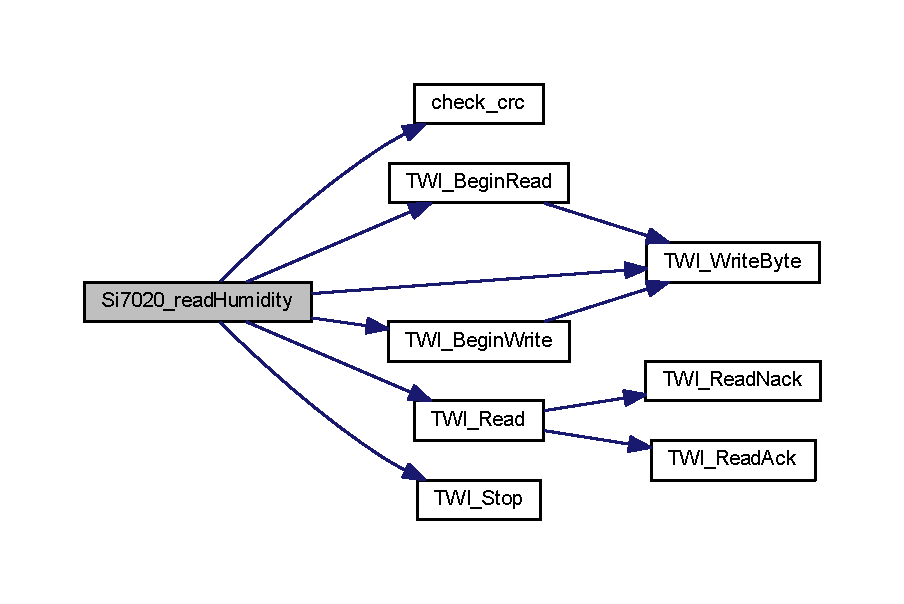
\includegraphics[width=350pt]{_si7020_8h_aebde99dd234f560632ecdbe126b67e05_cgraph}
\end{center}
\end{figure}


\hypertarget{_si7020_8h_ac561f9976fbf8f27a921f55fc402548d}{\index{Si7020.\-h@{Si7020.\-h}!Si7020\-\_\-read\-Temperature@{Si7020\-\_\-read\-Temperature}}
\index{Si7020\-\_\-read\-Temperature@{Si7020\-\_\-read\-Temperature}!Si7020.h@{Si7020.\-h}}
\subsubsection[{Si7020\-\_\-read\-Temperature}]{\setlength{\rightskip}{0pt plus 5cm}char Si7020\-\_\-read\-Temperature (
\begin{DoxyParamCaption}
\item[{unsigned char $\ast$}]{data, }
\item[{char}]{length}
\end{DoxyParamCaption}
)}}\label{_si7020_8h_ac561f9976fbf8f27a921f55fc402548d}


Read temperature from Si7020. 

\begin{DoxyReturn}{Returns}
status one if successfully read and crc check, otherwise return zero 
\end{DoxyReturn}


References check\-\_\-crc(), S\-I7020\-\_\-\-A\-D\-D\-R, S\-I7020\-\_\-\-T\-E\-M\-P\-E\-R\-A\-T\-U\-R\-E\-\_\-\-H\-O\-L\-D, status, T\-W\-I\-\_\-\-Begin\-Read(), T\-W\-I\-\_\-\-Begin\-Write(), T\-W\-I\-\_\-\-Read(), T\-W\-I\-\_\-\-R\-E\-C\-\_\-\-A\-C\-K, T\-W\-I\-\_\-\-S\-E\-N\-T\-\_\-\-A\-C\-K, T\-W\-I\-\_\-\-S\-L\-A\-R\-\_\-\-A\-C\-K, T\-W\-I\-\_\-\-Stop(), and T\-W\-I\-\_\-\-Write\-Byte().



Here is the call graph for this function\-:
\nopagebreak
\begin{figure}[H]
\begin{center}
\leavevmode
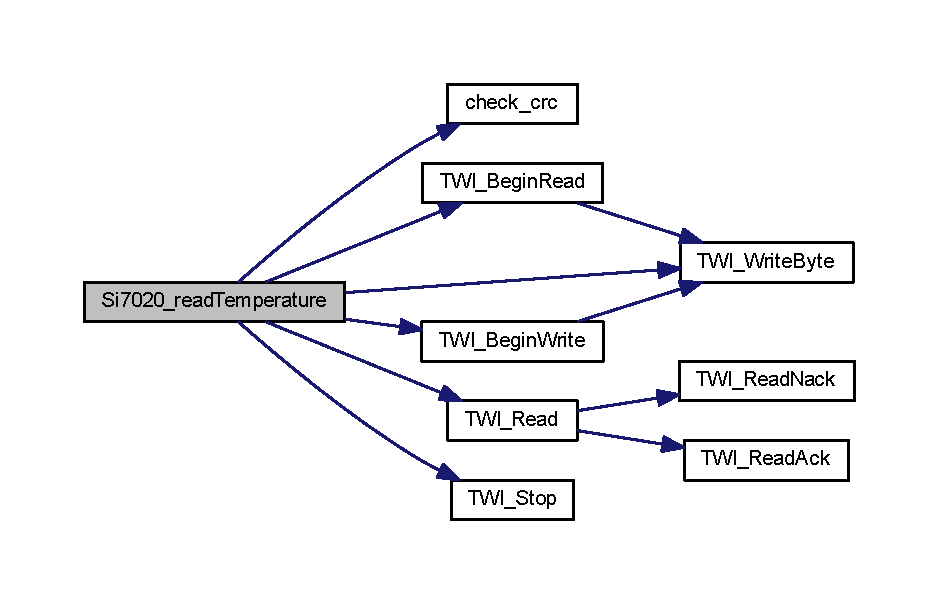
\includegraphics[width=350pt]{_si7020_8h_ac561f9976fbf8f27a921f55fc402548d_cgraph}
\end{center}
\end{figure}



\hypertarget{_t_g_s2600_8h}{\section{C\-:/\-Users/\-A\-B/\-Documents/\-Git\-Hub/\-A\-T\-M\-E\-L-\/\-A\-T\-M\-O\-S/\-A\-T\-M\-O\-S/devices/inc/\-T\-G\-S2600.h File Reference}
\label{_t_g_s2600_8h}\index{C\-:/\-Users/\-A\-B/\-Documents/\-Git\-Hub/\-A\-T\-M\-E\-L-\/\-A\-T\-M\-O\-S/\-A\-T\-M\-O\-S/devices/inc/\-T\-G\-S2600.\-h@{C\-:/\-Users/\-A\-B/\-Documents/\-Git\-Hub/\-A\-T\-M\-E\-L-\/\-A\-T\-M\-O\-S/\-A\-T\-M\-O\-S/devices/inc/\-T\-G\-S2600.\-h}}
}


Figaro T\-G\-S2600 air quality sensor libaray.  


This graph shows which files directly or indirectly include this file\-:
\nopagebreak
\begin{figure}[H]
\begin{center}
\leavevmode
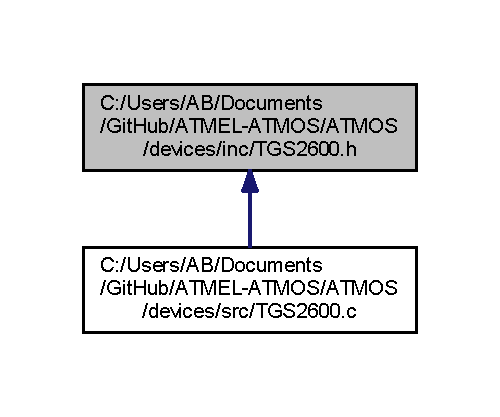
\includegraphics[width=240pt]{_t_g_s2600_8h__dep__incl}
\end{center}
\end{figure}
\subsection*{Functions}
\begin{DoxyCompactItemize}
\item 
void \hyperlink{_t_g_s2600_8h_ab6a71b827f15836749c426db0a6a789a}{T\-G\-S2600\-\_\-\-Init} (void)
\item 
void \hyperlink{_t_g_s2600_8h_a040d5bb1ee284f8005015e38e6aa6aaf}{T\-G\-S2600\-\_\-\-Turn\-On} (void)
\item 
void \hyperlink{_t_g_s2600_8h_a0a3db550cc96043f7990c02b22ae8ebb}{T\-G\-S2600\-\_\-\-Turn\-Off} (void)
\item 
float \hyperlink{_t_g_s2600_8h_a1d505496be4ec0580520ed3b1e933824}{T\-G\-S2600\-\_\-\-Get\-Resistance} (void)
\end{DoxyCompactItemize}


\subsection{Detailed Description}
Figaro T\-G\-S2600 air quality sensor libaray. Created\-: 4/10/2015 11\-:03\-:35 Author\-: Camden 

\subsection{Function Documentation}
\hypertarget{_t_g_s2600_8h_a1d505496be4ec0580520ed3b1e933824}{\index{T\-G\-S2600.\-h@{T\-G\-S2600.\-h}!T\-G\-S2600\-\_\-\-Get\-Resistance@{T\-G\-S2600\-\_\-\-Get\-Resistance}}
\index{T\-G\-S2600\-\_\-\-Get\-Resistance@{T\-G\-S2600\-\_\-\-Get\-Resistance}!TGS2600.h@{T\-G\-S2600.\-h}}
\subsubsection[{T\-G\-S2600\-\_\-\-Get\-Resistance}]{\setlength{\rightskip}{0pt plus 5cm}float T\-G\-S2600\-\_\-\-Get\-Resistance (
\begin{DoxyParamCaption}
\item[{void}]{}
\end{DoxyParamCaption}
)}}\label{_t_g_s2600_8h_a1d505496be4ec0580520ed3b1e933824}


References A\-D\-C1, A\-D\-C\-\_\-\-Convert(), A\-D\-C\-\_\-\-Reference(), and R\-E\-F\-E\-R\-E\-N\-C\-E\-\_\-\-A\-R\-E\-F.



Here is the call graph for this function\-:
\nopagebreak
\begin{figure}[H]
\begin{center}
\leavevmode
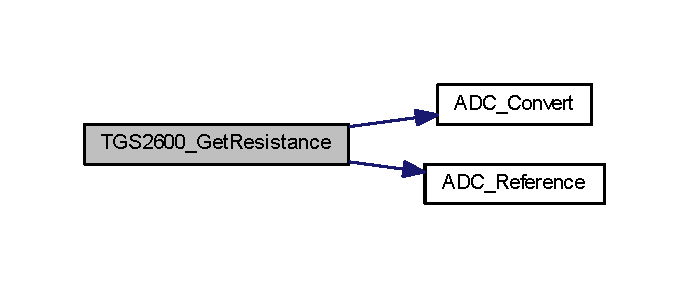
\includegraphics[width=330pt]{_t_g_s2600_8h_a1d505496be4ec0580520ed3b1e933824_cgraph}
\end{center}
\end{figure}


\hypertarget{_t_g_s2600_8h_ab6a71b827f15836749c426db0a6a789a}{\index{T\-G\-S2600.\-h@{T\-G\-S2600.\-h}!T\-G\-S2600\-\_\-\-Init@{T\-G\-S2600\-\_\-\-Init}}
\index{T\-G\-S2600\-\_\-\-Init@{T\-G\-S2600\-\_\-\-Init}!TGS2600.h@{T\-G\-S2600.\-h}}
\subsubsection[{T\-G\-S2600\-\_\-\-Init}]{\setlength{\rightskip}{0pt plus 5cm}void T\-G\-S2600\-\_\-\-Init (
\begin{DoxyParamCaption}
\item[{void}]{}
\end{DoxyParamCaption}
)}}\label{_t_g_s2600_8h_ab6a71b827f15836749c426db0a6a789a}


References T\-G\-S2600\-\_\-\-Turn\-On().



Here is the call graph for this function\-:
\nopagebreak
\begin{figure}[H]
\begin{center}
\leavevmode
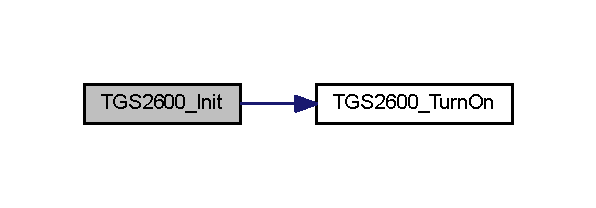
\includegraphics[width=286pt]{_t_g_s2600_8h_ab6a71b827f15836749c426db0a6a789a_cgraph}
\end{center}
\end{figure}


\hypertarget{_t_g_s2600_8h_a0a3db550cc96043f7990c02b22ae8ebb}{\index{T\-G\-S2600.\-h@{T\-G\-S2600.\-h}!T\-G\-S2600\-\_\-\-Turn\-Off@{T\-G\-S2600\-\_\-\-Turn\-Off}}
\index{T\-G\-S2600\-\_\-\-Turn\-Off@{T\-G\-S2600\-\_\-\-Turn\-Off}!TGS2600.h@{T\-G\-S2600.\-h}}
\subsubsection[{T\-G\-S2600\-\_\-\-Turn\-Off}]{\setlength{\rightskip}{0pt plus 5cm}void T\-G\-S2600\-\_\-\-Turn\-Off (
\begin{DoxyParamCaption}
\item[{void}]{}
\end{DoxyParamCaption}
)}}\label{_t_g_s2600_8h_a0a3db550cc96043f7990c02b22ae8ebb}
\hypertarget{_t_g_s2600_8h_a040d5bb1ee284f8005015e38e6aa6aaf}{\index{T\-G\-S2600.\-h@{T\-G\-S2600.\-h}!T\-G\-S2600\-\_\-\-Turn\-On@{T\-G\-S2600\-\_\-\-Turn\-On}}
\index{T\-G\-S2600\-\_\-\-Turn\-On@{T\-G\-S2600\-\_\-\-Turn\-On}!TGS2600.h@{T\-G\-S2600.\-h}}
\subsubsection[{T\-G\-S2600\-\_\-\-Turn\-On}]{\setlength{\rightskip}{0pt plus 5cm}void T\-G\-S2600\-\_\-\-Turn\-On (
\begin{DoxyParamCaption}
\item[{void}]{}
\end{DoxyParamCaption}
)}}\label{_t_g_s2600_8h_a040d5bb1ee284f8005015e38e6aa6aaf}


Referenced by T\-G\-S2600\-\_\-\-Init().



Here is the caller graph for this function\-:
\nopagebreak
\begin{figure}[H]
\begin{center}
\leavevmode
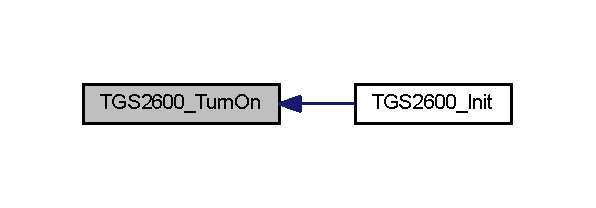
\includegraphics[width=286pt]{_t_g_s2600_8h_a040d5bb1ee284f8005015e38e6aa6aaf_icgraph}
\end{center}
\end{figure}



\hypertarget{_b_m_p280_8c}{\section{C\-:/\-Users/\-A\-B/\-Documents/\-Git\-Hub/\-A\-T\-M\-E\-L-\/\-A\-T\-M\-O\-S/\-A\-T\-M\-O\-S/devices/src/\-B\-M\-P280.c File Reference}
\label{_b_m_p280_8c}\index{C\-:/\-Users/\-A\-B/\-Documents/\-Git\-Hub/\-A\-T\-M\-E\-L-\/\-A\-T\-M\-O\-S/\-A\-T\-M\-O\-S/devices/src/\-B\-M\-P280.\-c@{C\-:/\-Users/\-A\-B/\-Documents/\-Git\-Hub/\-A\-T\-M\-E\-L-\/\-A\-T\-M\-O\-S/\-A\-T\-M\-O\-S/devices/src/\-B\-M\-P280.\-c}}
}


B\-M\-P280 Pressure Sensor Library implementation.  


{\ttfamily \#include \char`\"{}devices/inc/\-B\-M\-P280.\-h\char`\"{}}\\*
{\ttfamily \#include \char`\"{}drivers/inc/\-T\-W\-I.\-h\char`\"{}}\\*
{\ttfamily \#include \char`\"{}drivers/inc/usart0.\-h\char`\"{}}\\*
{\ttfamily \#include \char`\"{}math.\-h\char`\"{}}\\*
Include dependency graph for B\-M\-P280.\-c\-:
\nopagebreak
\begin{figure}[H]
\begin{center}
\leavevmode
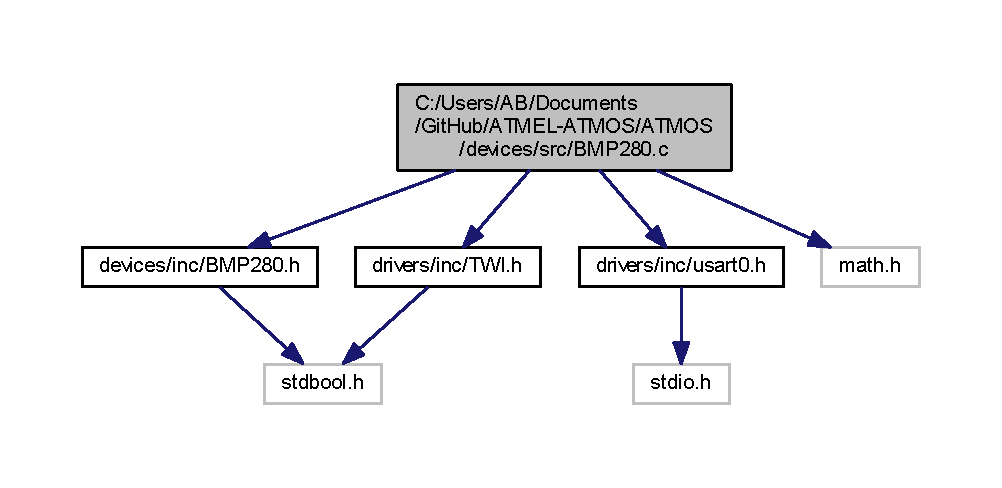
\includegraphics[width=350pt]{_b_m_p280_8c__incl}
\end{center}
\end{figure}
\subsection*{Functions}
\begin{DoxyCompactItemize}
\item 
static char \hyperlink{_b_m_p280_8c_a9dc83fe6c5b73afce7d6c95fdc8bf12e}{B\-M\-P280\-\_\-\-Read\-Int} (char address, int $\ast$val)
\begin{DoxyCompactList}\small\item\em Reads an int from the B\-M\-P280. \end{DoxyCompactList}\item 
static char \hyperlink{_b_m_p280_8c_a200056e2a6e922b99256963a78ec17ae}{B\-M\-P280\-\_\-\-Read\-U\-Int} (char address, unsigned int $\ast$val)
\begin{DoxyCompactList}\small\item\em Reads an unsigned int from the B\-M\-P280. \end{DoxyCompactList}\item 
static char \hyperlink{_b_m_p280_8c_a366477c92e35622e140f6e3e3d0ac141}{B\-M\-P280\-\_\-\-Read\-Bytes} (unsigned char $\ast$values, char length)
\begin{DoxyCompactList}\small\item\em Reads some bytes from the B\-M\-P280. \end{DoxyCompactList}\item 
static char \hyperlink{_b_m_p280_8c_a7634175c5e122cee3ae944189c389f7f}{B\-M\-P280\-\_\-\-Write\-Bytes} (unsigned char $\ast$values, char length)
\begin{DoxyCompactList}\small\item\em Reads some bytes from the B\-M\-P280. \end{DoxyCompactList}\item 
char \hyperlink{_b_m_p280_8c_a2d512d05a3f329da6e0bfb081a1f6685}{B\-M\-P280\-\_\-\-Init} (void)
\begin{DoxyCompactList}\small\item\em Initializes the B\-M\-P280 and reads the calibration data from the device. \end{DoxyCompactList}\item 
short \hyperlink{_b_m_p280_8c_a3af5a29c8b539b09126c1dd874a7e6c4}{B\-M\-P280\-\_\-\-Get\-Oversampling} (void)
\begin{DoxyCompactList}\small\item\em Gets the oversampling setting for the library. \end{DoxyCompactList}\item 
char \hyperlink{_b_m_p280_8c_ac56b30a97fa1388153530bb658a0ab3d}{B\-M\-P280\-\_\-\-Set\-Oversampling} (short oss)
\begin{DoxyCompactList}\small\item\em Sets the oversampling setting for the library. \end{DoxyCompactList}\item 
char \hyperlink{_b_m_p280_8c_a79fe54e0ce75dc946a3540bddd43e878}{B\-M\-P280\-\_\-\-Start\-Measurment} (void)
\begin{DoxyCompactList}\small\item\em Starts a measurement. \end{DoxyCompactList}\item 
char \hyperlink{_b_m_p280_8c_a008576c2ff8ad54b8886a77ce92d6a42}{B\-M\-P280\-\_\-\-Get\-Un\-P\-T} (double $\ast$u\-P, double $\ast$u\-T)
\begin{DoxyCompactList}\small\item\em Gets the uncalibrated temperature and pressure data. \end{DoxyCompactList}\item 
char \hyperlink{_b_m_p280_8c_ac9a59f23569a393dd0f9e33d57aa36d5}{B\-M\-P280\-\_\-\-Get\-Temperature\-And\-Pressure} (double $\ast$T, double $\ast$P)
\begin{DoxyCompactList}\small\item\em Gets temperature and pressure. \end{DoxyCompactList}\item 
char \hyperlink{_b_m_p280_8c_a44607ec60da729a027b3f2a0e5d63532}{B\-M\-P280\-\_\-\-Calc\-Temperature} (double $\ast$T, double $\ast$u\-T)
\begin{DoxyCompactList}\small\item\em Calculates temperature. \end{DoxyCompactList}\item 
char \hyperlink{_b_m_p280_8c_a3d508c8fcc342e017686eacd3159f893}{B\-M\-P280\-\_\-\-Calc\-Pressure} (double $\ast$P, double $\ast$u\-P)
\begin{DoxyCompactList}\small\item\em Calculates pressure. \end{DoxyCompactList}\item 
double \hyperlink{_b_m_p280_8c_ac1b069b6f5aab6238d8c4fa6ddc1d5ec}{B\-M\-P280\-\_\-\-Sealevel} (double P, double A)
\begin{DoxyCompactList}\small\item\em Calculates pressure at sea level given an altitude. \end{DoxyCompactList}\item 
double \hyperlink{_b_m_p280_8c_afebfcfaeec045e86479a110e03ac393d}{B\-M\-P280\-\_\-\-Altitude} (double P, double P0)
\begin{DoxyCompactList}\small\item\em Calculates altitude. \end{DoxyCompactList}\item 
char \hyperlink{_b_m_p280_8c_aeca60c0f36d134193d76793f85476422}{B\-M\-P280\-\_\-\-Get\-Error} (void)
\begin{DoxyCompactList}\small\item\em Returns the internal library error value. \end{DoxyCompactList}\end{DoxyCompactItemize}
\subsection*{Variables}
\begin{DoxyCompactItemize}
\item 
static int \hyperlink{_b_m_p280_8c_a3b17c748da9971b0089e0c914ed6ab91}{dig\-\_\-\-T2}
\item 
static int \hyperlink{_b_m_p280_8c_ae835e8b1e7ff5cb03d414e702c882e90}{dig\-\_\-\-T3}
\item 
static int \hyperlink{_b_m_p280_8c_a8c2786ed3ddd7ed0246fb1e6bab67391}{dig\-\_\-\-P2}
\item 
static int \hyperlink{_b_m_p280_8c_a7f9b0c21519941bca98b58cc5ac136d8}{dig\-\_\-\-P3}
\item 
static int \hyperlink{_b_m_p280_8c_af7c7ff3d06a32ef93f563662ea00d72e}{dig\-\_\-\-P4}
\item 
static int \hyperlink{_b_m_p280_8c_a0c84fc31f1fdbecbb8d860d553d350f1}{dig\-\_\-\-P5}
\item 
static int \hyperlink{_b_m_p280_8c_aa2b0df28fc7dd183923a20d88990078a}{dig\-\_\-\-P6}
\item 
static int \hyperlink{_b_m_p280_8c_acbc919cdec3dca3579eedc9e5749627c}{dig\-\_\-\-P7}
\item 
static int \hyperlink{_b_m_p280_8c_a411a8c30a36ad7c047f3406f4e065880}{dig\-\_\-\-P8}
\item 
static int \hyperlink{_b_m_p280_8c_ac36f2f0492522aaa0e9740b38d783fc9}{dig\-\_\-\-P9}
\begin{DoxyCompactList}\small\item\em Calibration values from the B\-M\-P280. \end{DoxyCompactList}\item 
static unsigned int \hyperlink{_b_m_p280_8c_aaf7e42bcadf006fc18be0805073e5f80}{dig\-\_\-\-P1}
\item 
static unsigned int \hyperlink{_b_m_p280_8c_ae10e166c5b8c3ea5677bc97ab2dee3cc}{dig\-\_\-\-T1}
\begin{DoxyCompactList}\small\item\em Calibration values from the B\-M\-P280. \end{DoxyCompactList}\item 
static short \hyperlink{_b_m_p280_8c_a386bf295f8efb8530c95f9b8d989732a}{oversampling}
\item 
static short \hyperlink{_b_m_p280_8c_af7f8339d15fb63f4333c507e3bdc908f}{oversampling\-\_\-t}
\begin{DoxyCompactList}\small\item\em Oversampling sertings. \end{DoxyCompactList}\item 
static long signed int \hyperlink{_b_m_p280_8c_ace4a7a7c43860cc488cc74bff162397c}{t\-\_\-fine}
\item 
static char \hyperlink{_b_m_p280_8c_a1b39a1a9b9888563c380903bcba6ecf4}{error}
\item 
static char \hyperlink{_b_m_p280_8c_a051c9e198ee930358372c407a17e8b78}{status}
\end{DoxyCompactItemize}


\subsection{Detailed Description}
B\-M\-P280 Pressure Sensor Library implementation. This library is intended only to work on the R\-E\-V1 base station, check \hyperlink{_b_m_p280_8h}{B\-M\-P280.\-h} for address defines and the like

Created\-: 2/10/2015 20\-:24\-:55 Author\-: Camden Miller 

\subsection{Function Documentation}
\hypertarget{_b_m_p280_8c_afebfcfaeec045e86479a110e03ac393d}{\index{B\-M\-P280.\-c@{B\-M\-P280.\-c}!B\-M\-P280\-\_\-\-Altitude@{B\-M\-P280\-\_\-\-Altitude}}
\index{B\-M\-P280\-\_\-\-Altitude@{B\-M\-P280\-\_\-\-Altitude}!BMP280.c@{B\-M\-P280.\-c}}
\subsubsection[{B\-M\-P280\-\_\-\-Altitude}]{\setlength{\rightskip}{0pt plus 5cm}double B\-M\-P280\-\_\-\-Altitude (
\begin{DoxyParamCaption}
\item[{double}]{P, }
\item[{double}]{P0}
\end{DoxyParamCaption}
)}}\label{_b_m_p280_8c_afebfcfaeec045e86479a110e03ac393d}


Calculates altitude. 


\begin{DoxyParams}[1]{Parameters}
\mbox{\tt in}  & {\em pressure} & reading \\
\hline
\mbox{\tt in}  & {\em sea} & level pressure \\
\hline
\end{DoxyParams}
\begin{DoxyReturn}{Returns}
the corrected reading 
\end{DoxyReturn}
\hypertarget{_b_m_p280_8c_a3d508c8fcc342e017686eacd3159f893}{\index{B\-M\-P280.\-c@{B\-M\-P280.\-c}!B\-M\-P280\-\_\-\-Calc\-Pressure@{B\-M\-P280\-\_\-\-Calc\-Pressure}}
\index{B\-M\-P280\-\_\-\-Calc\-Pressure@{B\-M\-P280\-\_\-\-Calc\-Pressure}!BMP280.c@{B\-M\-P280.\-c}}
\subsubsection[{B\-M\-P280\-\_\-\-Calc\-Pressure}]{\setlength{\rightskip}{0pt plus 5cm}char B\-M\-P280\-\_\-\-Calc\-Pressure (
\begin{DoxyParamCaption}
\item[{double $\ast$}]{P, }
\item[{double $\ast$}]{u\-P}
\end{DoxyParamCaption}
)}}\label{_b_m_p280_8c_a3d508c8fcc342e017686eacd3159f893}


Calculates pressure. 


\begin{DoxyParams}[1]{Parameters}
\mbox{\tt out}  & {\em pointer} & to a place to store the pressure data \\
\hline
\mbox{\tt in}  & {\em pointer} & to the uncalibrated pressure data \\
\hline
\end{DoxyParams}
\begin{DoxyReturn}{Returns}
status 
\end{DoxyReturn}


References dig\-\_\-\-P1, dig\-\_\-\-P2, dig\-\_\-\-P3, dig\-\_\-\-P4, dig\-\_\-\-P5, dig\-\_\-\-P6, dig\-\_\-\-P7, dig\-\_\-\-P8, dig\-\_\-\-P9, and t\-\_\-fine.



Referenced by B\-M\-P280\-\_\-\-Get\-Temperature\-And\-Pressure().



Here is the caller graph for this function\-:
\nopagebreak
\begin{figure}[H]
\begin{center}
\leavevmode
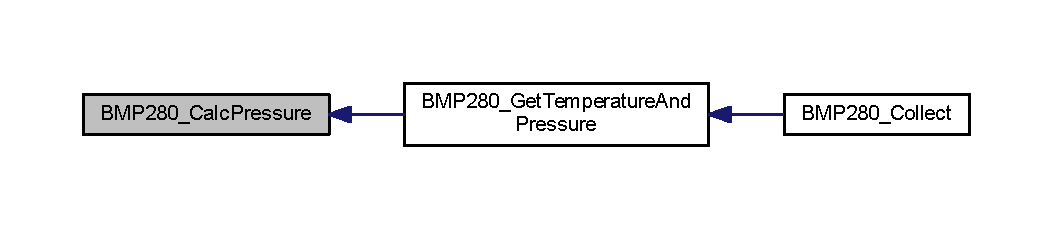
\includegraphics[width=350pt]{_b_m_p280_8c_a3d508c8fcc342e017686eacd3159f893_icgraph}
\end{center}
\end{figure}


\hypertarget{_b_m_p280_8c_a44607ec60da729a027b3f2a0e5d63532}{\index{B\-M\-P280.\-c@{B\-M\-P280.\-c}!B\-M\-P280\-\_\-\-Calc\-Temperature@{B\-M\-P280\-\_\-\-Calc\-Temperature}}
\index{B\-M\-P280\-\_\-\-Calc\-Temperature@{B\-M\-P280\-\_\-\-Calc\-Temperature}!BMP280.c@{B\-M\-P280.\-c}}
\subsubsection[{B\-M\-P280\-\_\-\-Calc\-Temperature}]{\setlength{\rightskip}{0pt plus 5cm}char B\-M\-P280\-\_\-\-Calc\-Temperature (
\begin{DoxyParamCaption}
\item[{double $\ast$}]{T, }
\item[{double $\ast$}]{u\-T}
\end{DoxyParamCaption}
)}}\label{_b_m_p280_8c_a44607ec60da729a027b3f2a0e5d63532}


Calculates temperature. 


\begin{DoxyParams}[1]{Parameters}
\mbox{\tt out}  & {\em pointer} & to a place to store the temperature data \\
\hline
\mbox{\tt in}  & {\em pointer} & to the uncalibrated temperature data \\
\hline
\end{DoxyParams}
\begin{DoxyReturn}{Returns}
status 
\end{DoxyReturn}


References dig\-\_\-\-T1, dig\-\_\-\-T2, dig\-\_\-\-T3, and t\-\_\-fine.



Referenced by B\-M\-P280\-\_\-\-Get\-Temperature\-And\-Pressure().



Here is the caller graph for this function\-:
\nopagebreak
\begin{figure}[H]
\begin{center}
\leavevmode
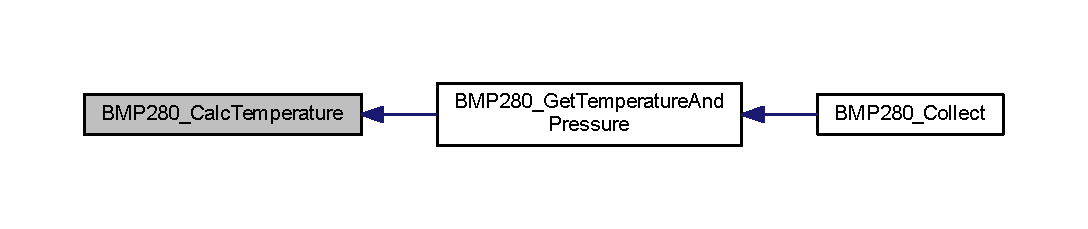
\includegraphics[width=350pt]{_b_m_p280_8c_a44607ec60da729a027b3f2a0e5d63532_icgraph}
\end{center}
\end{figure}


\hypertarget{_b_m_p280_8c_aeca60c0f36d134193d76793f85476422}{\index{B\-M\-P280.\-c@{B\-M\-P280.\-c}!B\-M\-P280\-\_\-\-Get\-Error@{B\-M\-P280\-\_\-\-Get\-Error}}
\index{B\-M\-P280\-\_\-\-Get\-Error@{B\-M\-P280\-\_\-\-Get\-Error}!BMP280.c@{B\-M\-P280.\-c}}
\subsubsection[{B\-M\-P280\-\_\-\-Get\-Error}]{\setlength{\rightskip}{0pt plus 5cm}char B\-M\-P280\-\_\-\-Get\-Error (
\begin{DoxyParamCaption}
\item[{void}]{}
\end{DoxyParamCaption}
)}}\label{_b_m_p280_8c_aeca60c0f36d134193d76793f85476422}


Returns the internal library error value. 


\begin{DoxyParams}[1]{Parameters}
\mbox{\tt in}  & {\em pressure} & reading \\
\hline
\mbox{\tt in}  & {\em sea} & level pressure \\
\hline
\end{DoxyParams}
\begin{DoxyReturn}{Returns}
error value 
\end{DoxyReturn}


References error.

\hypertarget{_b_m_p280_8c_a3af5a29c8b539b09126c1dd874a7e6c4}{\index{B\-M\-P280.\-c@{B\-M\-P280.\-c}!B\-M\-P280\-\_\-\-Get\-Oversampling@{B\-M\-P280\-\_\-\-Get\-Oversampling}}
\index{B\-M\-P280\-\_\-\-Get\-Oversampling@{B\-M\-P280\-\_\-\-Get\-Oversampling}!BMP280.c@{B\-M\-P280.\-c}}
\subsubsection[{B\-M\-P280\-\_\-\-Get\-Oversampling}]{\setlength{\rightskip}{0pt plus 5cm}short B\-M\-P280\-\_\-\-Get\-Oversampling (
\begin{DoxyParamCaption}
\item[{void}]{}
\end{DoxyParamCaption}
)}}\label{_b_m_p280_8c_a3af5a29c8b539b09126c1dd874a7e6c4}


Gets the oversampling setting for the library. 

\begin{DoxyReturn}{Returns}
oversampling 
\end{DoxyReturn}


References oversampling.

\hypertarget{_b_m_p280_8c_ac9a59f23569a393dd0f9e33d57aa36d5}{\index{B\-M\-P280.\-c@{B\-M\-P280.\-c}!B\-M\-P280\-\_\-\-Get\-Temperature\-And\-Pressure@{B\-M\-P280\-\_\-\-Get\-Temperature\-And\-Pressure}}
\index{B\-M\-P280\-\_\-\-Get\-Temperature\-And\-Pressure@{B\-M\-P280\-\_\-\-Get\-Temperature\-And\-Pressure}!BMP280.c@{B\-M\-P280.\-c}}
\subsubsection[{B\-M\-P280\-\_\-\-Get\-Temperature\-And\-Pressure}]{\setlength{\rightskip}{0pt plus 5cm}char B\-M\-P280\-\_\-\-Get\-Temperature\-And\-Pressure (
\begin{DoxyParamCaption}
\item[{double $\ast$}]{T, }
\item[{double $\ast$}]{P}
\end{DoxyParamCaption}
)}}\label{_b_m_p280_8c_ac9a59f23569a393dd0f9e33d57aa36d5}


Gets temperature and pressure. 


\begin{DoxyParams}[1]{Parameters}
\mbox{\tt out}  & {\em pointer} & to a place to store the pressure data \\
\hline
\mbox{\tt out}  & {\em pointer} & to a place to store the temperature data \\
\hline
\end{DoxyParams}
\begin{DoxyReturn}{Returns}
status 
\end{DoxyReturn}


References B\-M\-P280\-\_\-\-Calc\-Pressure(), B\-M\-P280\-\_\-\-Calc\-Temperature(), B\-M\-P280\-\_\-\-Get\-Un\-P\-T(), and error.



Referenced by B\-M\-P280\-\_\-\-Collect().



Here is the call graph for this function\-:
\nopagebreak
\begin{figure}[H]
\begin{center}
\leavevmode
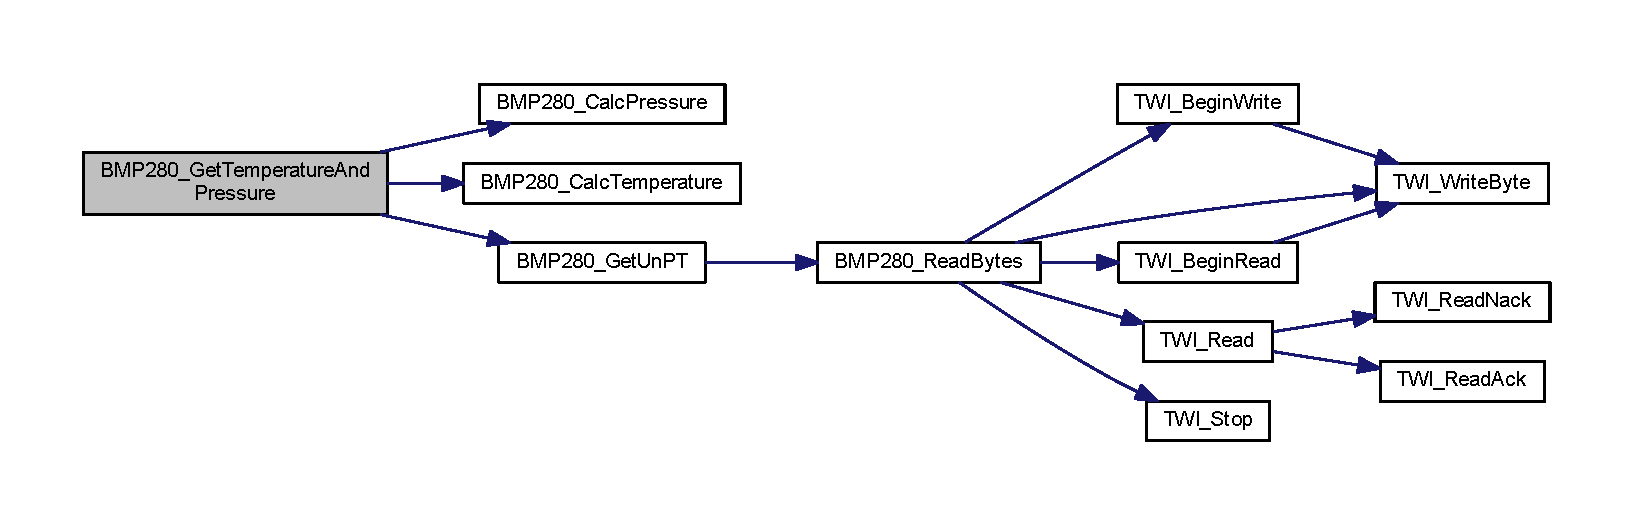
\includegraphics[width=350pt]{_b_m_p280_8c_ac9a59f23569a393dd0f9e33d57aa36d5_cgraph}
\end{center}
\end{figure}




Here is the caller graph for this function\-:
\nopagebreak
\begin{figure}[H]
\begin{center}
\leavevmode
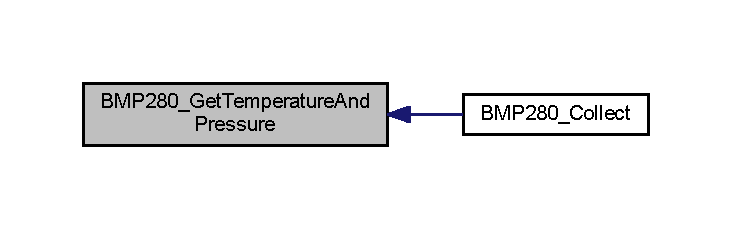
\includegraphics[width=350pt]{_b_m_p280_8c_ac9a59f23569a393dd0f9e33d57aa36d5_icgraph}
\end{center}
\end{figure}


\hypertarget{_b_m_p280_8c_a008576c2ff8ad54b8886a77ce92d6a42}{\index{B\-M\-P280.\-c@{B\-M\-P280.\-c}!B\-M\-P280\-\_\-\-Get\-Un\-P\-T@{B\-M\-P280\-\_\-\-Get\-Un\-P\-T}}
\index{B\-M\-P280\-\_\-\-Get\-Un\-P\-T@{B\-M\-P280\-\_\-\-Get\-Un\-P\-T}!BMP280.c@{B\-M\-P280.\-c}}
\subsubsection[{B\-M\-P280\-\_\-\-Get\-Un\-P\-T}]{\setlength{\rightskip}{0pt plus 5cm}char B\-M\-P280\-\_\-\-Get\-Un\-P\-T (
\begin{DoxyParamCaption}
\item[{double $\ast$}]{u\-P, }
\item[{double $\ast$}]{u\-T}
\end{DoxyParamCaption}
)}}\label{_b_m_p280_8c_a008576c2ff8ad54b8886a77ce92d6a42}


Gets the uncalibrated temperature and pressure data. 


\begin{DoxyParams}[1]{Parameters}
\mbox{\tt out}  & {\em pointer} & to a place to store the pressure data \\
\hline
\mbox{\tt out}  & {\em pointer} & to a place to store the temperature data \\
\hline
\end{DoxyParams}
\begin{DoxyReturn}{Returns}
status 
\end{DoxyReturn}


References B\-M\-P280\-\_\-\-Read\-Bytes(), and B\-M\-P280\-\_\-\-R\-E\-G\-\_\-\-R\-E\-S\-U\-L\-T\-\_\-\-P\-R\-E\-S\-S\-U\-R\-E.



Referenced by B\-M\-P280\-\_\-\-Get\-Temperature\-And\-Pressure().



Here is the call graph for this function\-:
\nopagebreak
\begin{figure}[H]
\begin{center}
\leavevmode
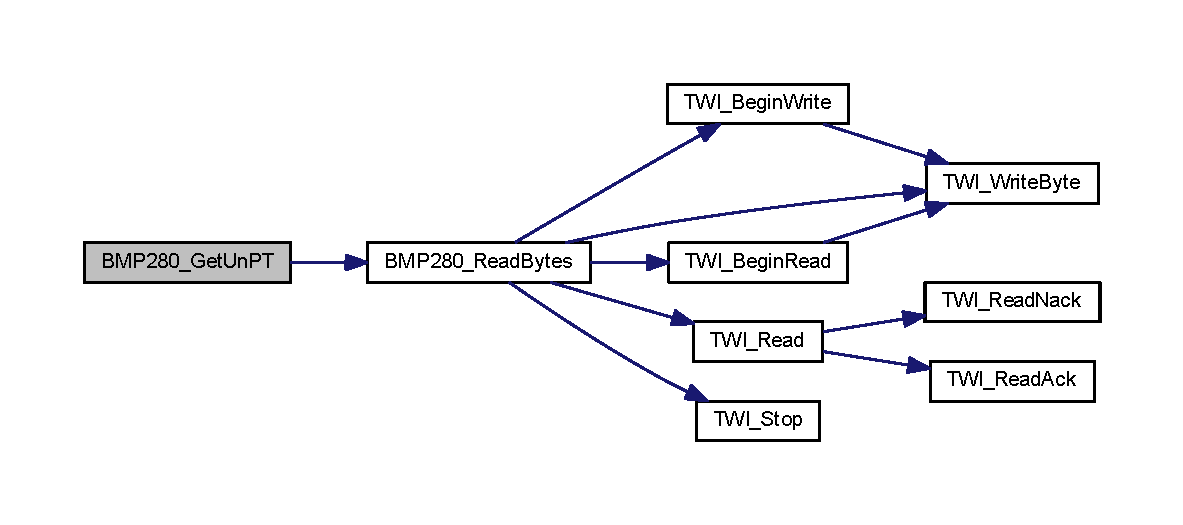
\includegraphics[width=350pt]{_b_m_p280_8c_a008576c2ff8ad54b8886a77ce92d6a42_cgraph}
\end{center}
\end{figure}




Here is the caller graph for this function\-:
\nopagebreak
\begin{figure}[H]
\begin{center}
\leavevmode
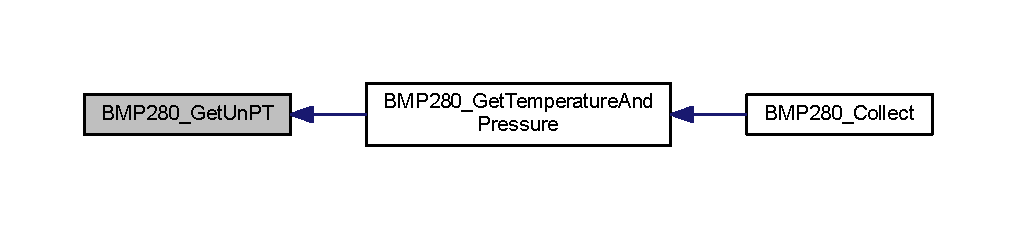
\includegraphics[width=350pt]{_b_m_p280_8c_a008576c2ff8ad54b8886a77ce92d6a42_icgraph}
\end{center}
\end{figure}


\hypertarget{_b_m_p280_8c_a2d512d05a3f329da6e0bfb081a1f6685}{\index{B\-M\-P280.\-c@{B\-M\-P280.\-c}!B\-M\-P280\-\_\-\-Init@{B\-M\-P280\-\_\-\-Init}}
\index{B\-M\-P280\-\_\-\-Init@{B\-M\-P280\-\_\-\-Init}!BMP280.c@{B\-M\-P280.\-c}}
\subsubsection[{B\-M\-P280\-\_\-\-Init}]{\setlength{\rightskip}{0pt plus 5cm}char B\-M\-P280\-\_\-\-Init (
\begin{DoxyParamCaption}
\item[{void}]{}
\end{DoxyParamCaption}
)}}\label{_b_m_p280_8c_a2d512d05a3f329da6e0bfb081a1f6685}


Initializes the B\-M\-P280 and reads the calibration data from the device. 

\begin{DoxyReturn}{Returns}
status (zero on failure, nonzero otherwise) 
\end{DoxyReturn}


References B\-M\-P280\-\_\-\-Read\-Int(), B\-M\-P280\-\_\-\-Read\-U\-Int(), dig\-\_\-\-P1, dig\-\_\-\-P2, dig\-\_\-\-P3, dig\-\_\-\-P4, dig\-\_\-\-P5, dig\-\_\-\-P6, dig\-\_\-\-P7, dig\-\_\-\-P8, dig\-\_\-\-P9, dig\-\_\-\-T1, dig\-\_\-\-T2, and dig\-\_\-\-T3.



Referenced by A\-P\-P\-\_\-\-Init().



Here is the call graph for this function\-:
\nopagebreak
\begin{figure}[H]
\begin{center}
\leavevmode
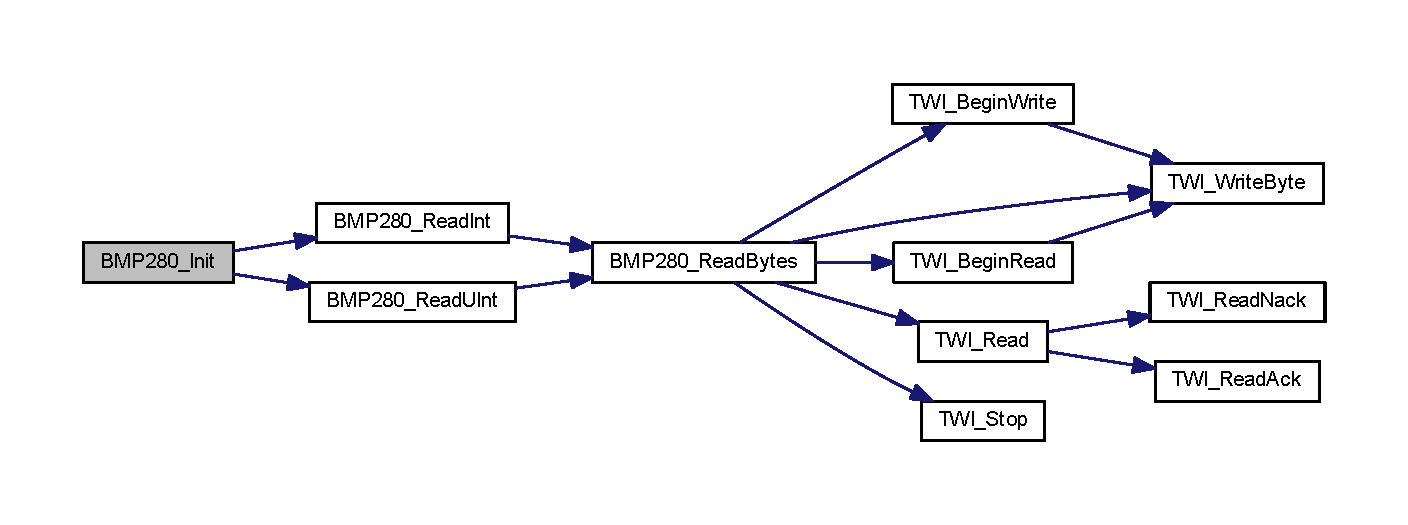
\includegraphics[width=350pt]{_b_m_p280_8c_a2d512d05a3f329da6e0bfb081a1f6685_cgraph}
\end{center}
\end{figure}




Here is the caller graph for this function\-:
\nopagebreak
\begin{figure}[H]
\begin{center}
\leavevmode
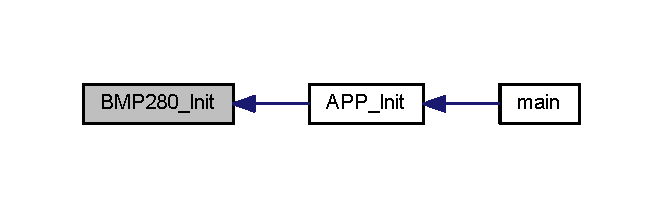
\includegraphics[width=318pt]{_b_m_p280_8c_a2d512d05a3f329da6e0bfb081a1f6685_icgraph}
\end{center}
\end{figure}


\hypertarget{_b_m_p280_8c_a366477c92e35622e140f6e3e3d0ac141}{\index{B\-M\-P280.\-c@{B\-M\-P280.\-c}!B\-M\-P280\-\_\-\-Read\-Bytes@{B\-M\-P280\-\_\-\-Read\-Bytes}}
\index{B\-M\-P280\-\_\-\-Read\-Bytes@{B\-M\-P280\-\_\-\-Read\-Bytes}!BMP280.c@{B\-M\-P280.\-c}}
\subsubsection[{B\-M\-P280\-\_\-\-Read\-Bytes}]{\setlength{\rightskip}{0pt plus 5cm}static char B\-M\-P280\-\_\-\-Read\-Bytes (
\begin{DoxyParamCaption}
\item[{unsigned char $\ast$}]{values, }
\item[{char}]{length}
\end{DoxyParamCaption}
)\hspace{0.3cm}{\ttfamily [static]}}}\label{_b_m_p280_8c_a366477c92e35622e140f6e3e3d0ac141}


Reads some bytes from the B\-M\-P280. 

Has no buffer overrun protection 
\begin{DoxyParams}[1]{Parameters}
\mbox{\tt in}  & {\em $\ast$values} & pointer to an array to store the bytes, put the starting register in values\mbox{[}0\mbox{]} \\
\hline
\mbox{\tt in}  & {\em length} & how many bytes to read \\
\hline
\end{DoxyParams}
\begin{DoxyReturn}{Returns}
status (zero on failure, nonzero otherwise) 
\end{DoxyReturn}


References B\-M\-P280\-\_\-\-A\-D\-D\-R, status, T\-W\-I\-\_\-\-Begin\-Read(), T\-W\-I\-\_\-\-Begin\-Write(), T\-W\-I\-\_\-\-Read(), T\-W\-I\-\_\-\-R\-E\-C\-\_\-\-N\-A\-C\-K, T\-W\-I\-\_\-\-S\-L\-A\-R\-\_\-\-A\-C\-K, T\-W\-I\-\_\-\-Stop(), T\-W\-I\-\_\-\-Write\-Byte(), and T\-W\-S\-R\-\_\-\-M\-A\-S\-K.



Referenced by B\-M\-P280\-\_\-\-Get\-Un\-P\-T(), B\-M\-P280\-\_\-\-Read\-Int(), and B\-M\-P280\-\_\-\-Read\-U\-Int().



Here is the call graph for this function\-:
\nopagebreak
\begin{figure}[H]
\begin{center}
\leavevmode
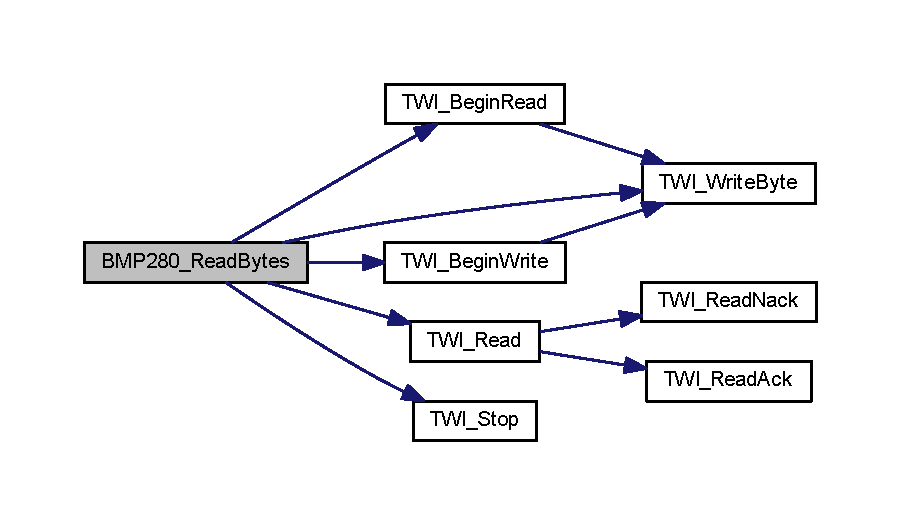
\includegraphics[width=350pt]{_b_m_p280_8c_a366477c92e35622e140f6e3e3d0ac141_cgraph}
\end{center}
\end{figure}




Here is the caller graph for this function\-:
\nopagebreak
\begin{figure}[H]
\begin{center}
\leavevmode
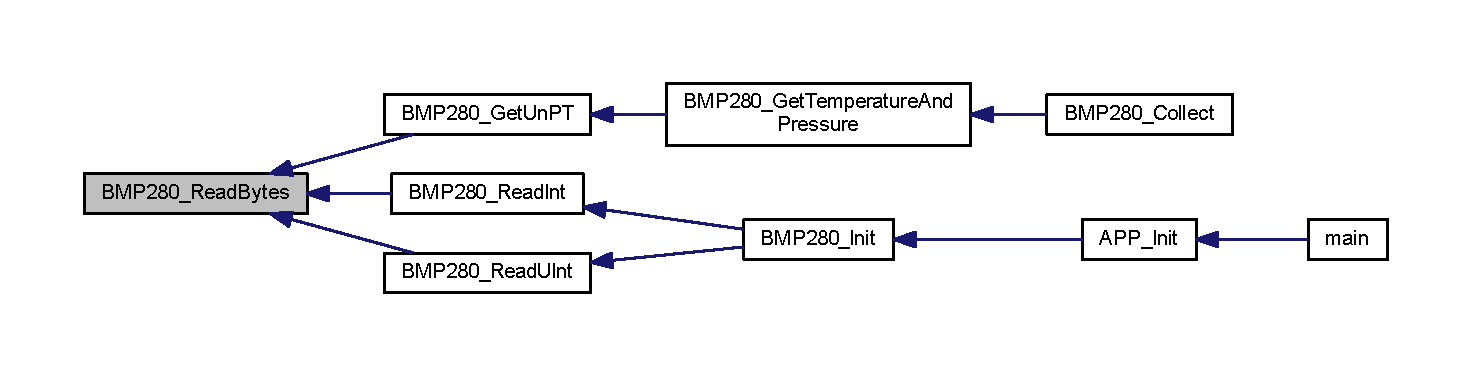
\includegraphics[width=350pt]{_b_m_p280_8c_a366477c92e35622e140f6e3e3d0ac141_icgraph}
\end{center}
\end{figure}


\hypertarget{_b_m_p280_8c_a9dc83fe6c5b73afce7d6c95fdc8bf12e}{\index{B\-M\-P280.\-c@{B\-M\-P280.\-c}!B\-M\-P280\-\_\-\-Read\-Int@{B\-M\-P280\-\_\-\-Read\-Int}}
\index{B\-M\-P280\-\_\-\-Read\-Int@{B\-M\-P280\-\_\-\-Read\-Int}!BMP280.c@{B\-M\-P280.\-c}}
\subsubsection[{B\-M\-P280\-\_\-\-Read\-Int}]{\setlength{\rightskip}{0pt plus 5cm}static char B\-M\-P280\-\_\-\-Read\-Int (
\begin{DoxyParamCaption}
\item[{char}]{address, }
\item[{int $\ast$}]{val}
\end{DoxyParamCaption}
)\hspace{0.3cm}{\ttfamily [static]}}}\label{_b_m_p280_8c_a9dc83fe6c5b73afce7d6c95fdc8bf12e}


Reads an int from the B\-M\-P280. 


\begin{DoxyParams}[1]{Parameters}
\mbox{\tt in}  & {\em address} & The register address of the first byte of the uint \\
\hline
\mbox{\tt out}  & {\em val$\ast$} & A pointer to a uint to store the received data to \\
\hline
\end{DoxyParams}
\begin{DoxyReturn}{Returns}
status (zero on failure, nonzero otherwise) 
\end{DoxyReturn}


References B\-M\-P280\-\_\-\-Read\-Bytes().



Referenced by B\-M\-P280\-\_\-\-Init().



Here is the call graph for this function\-:
\nopagebreak
\begin{figure}[H]
\begin{center}
\leavevmode
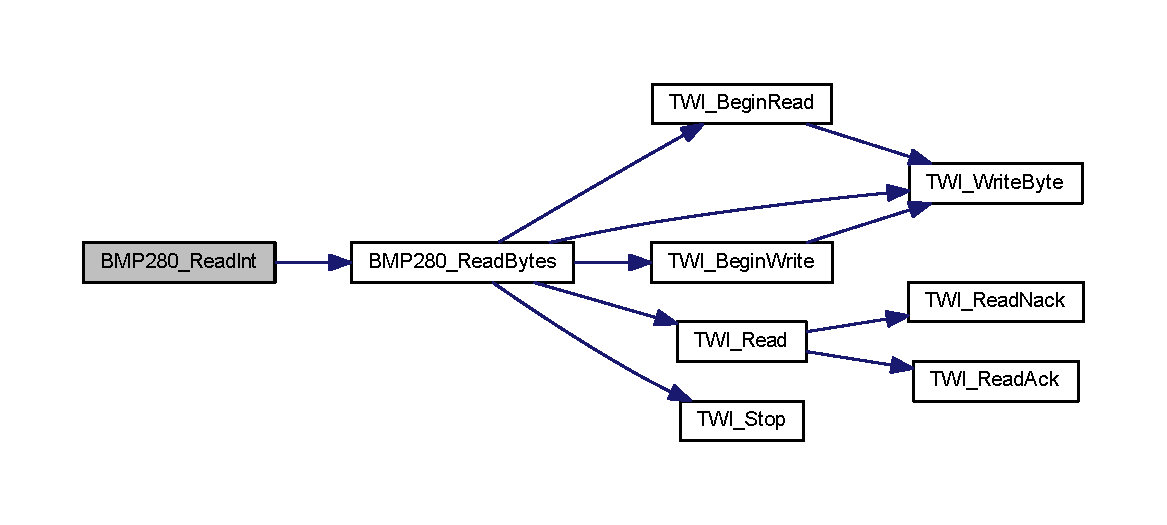
\includegraphics[width=350pt]{_b_m_p280_8c_a9dc83fe6c5b73afce7d6c95fdc8bf12e_cgraph}
\end{center}
\end{figure}




Here is the caller graph for this function\-:
\nopagebreak
\begin{figure}[H]
\begin{center}
\leavevmode
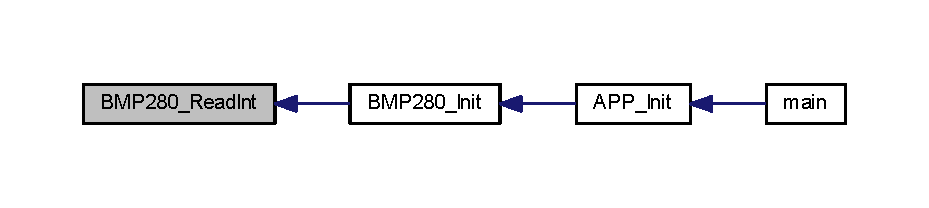
\includegraphics[width=350pt]{_b_m_p280_8c_a9dc83fe6c5b73afce7d6c95fdc8bf12e_icgraph}
\end{center}
\end{figure}


\hypertarget{_b_m_p280_8c_a200056e2a6e922b99256963a78ec17ae}{\index{B\-M\-P280.\-c@{B\-M\-P280.\-c}!B\-M\-P280\-\_\-\-Read\-U\-Int@{B\-M\-P280\-\_\-\-Read\-U\-Int}}
\index{B\-M\-P280\-\_\-\-Read\-U\-Int@{B\-M\-P280\-\_\-\-Read\-U\-Int}!BMP280.c@{B\-M\-P280.\-c}}
\subsubsection[{B\-M\-P280\-\_\-\-Read\-U\-Int}]{\setlength{\rightskip}{0pt plus 5cm}static char B\-M\-P280\-\_\-\-Read\-U\-Int (
\begin{DoxyParamCaption}
\item[{char}]{address, }
\item[{unsigned int $\ast$}]{val}
\end{DoxyParamCaption}
)\hspace{0.3cm}{\ttfamily [static]}}}\label{_b_m_p280_8c_a200056e2a6e922b99256963a78ec17ae}


Reads an unsigned int from the B\-M\-P280. 


\begin{DoxyParams}[1]{Parameters}
\mbox{\tt in}  & {\em address} & The register address of the first byte of the uint \\
\hline
\mbox{\tt out}  & {\em val$\ast$} & A pointer to a uint to store the received data to \\
\hline
\end{DoxyParams}
\begin{DoxyReturn}{Returns}
status (zero on failure, nonzero otherwise) 
\end{DoxyReturn}


References B\-M\-P280\-\_\-\-Read\-Bytes().



Referenced by B\-M\-P280\-\_\-\-Init().



Here is the call graph for this function\-:
\nopagebreak
\begin{figure}[H]
\begin{center}
\leavevmode
\includegraphics[width=350pt]{_b_m_p280_8c_a200056e2a6e922b99256963a78ec17ae_cgraph}
\end{center}
\end{figure}




Here is the caller graph for this function\-:
\nopagebreak
\begin{figure}[H]
\begin{center}
\leavevmode
\includegraphics[width=350pt]{_b_m_p280_8c_a200056e2a6e922b99256963a78ec17ae_icgraph}
\end{center}
\end{figure}


\hypertarget{_b_m_p280_8c_ac1b069b6f5aab6238d8c4fa6ddc1d5ec}{\index{B\-M\-P280.\-c@{B\-M\-P280.\-c}!B\-M\-P280\-\_\-\-Sealevel@{B\-M\-P280\-\_\-\-Sealevel}}
\index{B\-M\-P280\-\_\-\-Sealevel@{B\-M\-P280\-\_\-\-Sealevel}!BMP280.c@{B\-M\-P280.\-c}}
\subsubsection[{B\-M\-P280\-\_\-\-Sealevel}]{\setlength{\rightskip}{0pt plus 5cm}double B\-M\-P280\-\_\-\-Sealevel (
\begin{DoxyParamCaption}
\item[{double}]{P, }
\item[{double}]{A}
\end{DoxyParamCaption}
)}}\label{_b_m_p280_8c_ac1b069b6f5aab6238d8c4fa6ddc1d5ec}


Calculates pressure at sea level given an altitude. 


\begin{DoxyParams}[1]{Parameters}
\mbox{\tt in}  & {\em pressure} & reading \\
\hline
\mbox{\tt in}  & {\em altitude} & \\
\hline
\end{DoxyParams}
\begin{DoxyReturn}{Returns}
the corrected reading 
\end{DoxyReturn}
\hypertarget{_b_m_p280_8c_ac56b30a97fa1388153530bb658a0ab3d}{\index{B\-M\-P280.\-c@{B\-M\-P280.\-c}!B\-M\-P280\-\_\-\-Set\-Oversampling@{B\-M\-P280\-\_\-\-Set\-Oversampling}}
\index{B\-M\-P280\-\_\-\-Set\-Oversampling@{B\-M\-P280\-\_\-\-Set\-Oversampling}!BMP280.c@{B\-M\-P280.\-c}}
\subsubsection[{B\-M\-P280\-\_\-\-Set\-Oversampling}]{\setlength{\rightskip}{0pt plus 5cm}char B\-M\-P280\-\_\-\-Set\-Oversampling (
\begin{DoxyParamCaption}
\item[{short}]{oss}
\end{DoxyParamCaption}
)}}\label{_b_m_p280_8c_ac56b30a97fa1388153530bb658a0ab3d}


Sets the oversampling setting for the library. 


\begin{DoxyParams}[1]{Parameters}
\mbox{\tt in}  & {\em oss} & Oversampling setting \\
\hline
\end{DoxyParams}
\begin{DoxyReturn}{Returns}
1 
\end{DoxyReturn}


References oversampling.



Referenced by A\-P\-P\-\_\-\-Init().



Here is the caller graph for this function\-:
\nopagebreak
\begin{figure}[H]
\begin{center}
\leavevmode
\includegraphics[width=350pt]{_b_m_p280_8c_ac56b30a97fa1388153530bb658a0ab3d_icgraph}
\end{center}
\end{figure}


\hypertarget{_b_m_p280_8c_a79fe54e0ce75dc946a3540bddd43e878}{\index{B\-M\-P280.\-c@{B\-M\-P280.\-c}!B\-M\-P280\-\_\-\-Start\-Measurment@{B\-M\-P280\-\_\-\-Start\-Measurment}}
\index{B\-M\-P280\-\_\-\-Start\-Measurment@{B\-M\-P280\-\_\-\-Start\-Measurment}!BMP280.c@{B\-M\-P280.\-c}}
\subsubsection[{B\-M\-P280\-\_\-\-Start\-Measurment}]{\setlength{\rightskip}{0pt plus 5cm}char B\-M\-P280\-\_\-\-Start\-Measurment (
\begin{DoxyParamCaption}
\item[{void}]{}
\end{DoxyParamCaption}
)}}\label{_b_m_p280_8c_a79fe54e0ce75dc946a3540bddd43e878}


Starts a measurement. 

\begin{DoxyReturn}{Returns}
time to wait for result (in ms) 
\end{DoxyReturn}


References B\-M\-P280\-\_\-\-C\-O\-M\-M\-A\-N\-D\-\_\-\-P\-R\-E\-S\-S\-U\-R\-E0, B\-M\-P280\-\_\-\-C\-O\-M\-M\-A\-N\-D\-\_\-\-P\-R\-E\-S\-S\-U\-R\-E1, B\-M\-P280\-\_\-\-C\-O\-M\-M\-A\-N\-D\-\_\-\-P\-R\-E\-S\-S\-U\-R\-E2, B\-M\-P280\-\_\-\-C\-O\-M\-M\-A\-N\-D\-\_\-\-P\-R\-E\-S\-S\-U\-R\-E3, B\-M\-P280\-\_\-\-C\-O\-M\-M\-A\-N\-D\-\_\-\-P\-R\-E\-S\-S\-U\-R\-E4, B\-M\-P280\-\_\-\-R\-E\-G\-\_\-\-C\-O\-N\-T\-R\-O\-L, B\-M\-P280\-\_\-\-Write\-Bytes(), delay, oversampling, and oversampling\-\_\-t.



Referenced by B\-M\-P280\-\_\-\-Request().



Here is the call graph for this function\-:
\nopagebreak
\begin{figure}[H]
\begin{center}
\leavevmode
\includegraphics[width=350pt]{_b_m_p280_8c_a79fe54e0ce75dc946a3540bddd43e878_cgraph}
\end{center}
\end{figure}




Here is the caller graph for this function\-:
\nopagebreak
\begin{figure}[H]
\begin{center}
\leavevmode
\includegraphics[width=346pt]{_b_m_p280_8c_a79fe54e0ce75dc946a3540bddd43e878_icgraph}
\end{center}
\end{figure}


\hypertarget{_b_m_p280_8c_a7634175c5e122cee3ae944189c389f7f}{\index{B\-M\-P280.\-c@{B\-M\-P280.\-c}!B\-M\-P280\-\_\-\-Write\-Bytes@{B\-M\-P280\-\_\-\-Write\-Bytes}}
\index{B\-M\-P280\-\_\-\-Write\-Bytes@{B\-M\-P280\-\_\-\-Write\-Bytes}!BMP280.c@{B\-M\-P280.\-c}}
\subsubsection[{B\-M\-P280\-\_\-\-Write\-Bytes}]{\setlength{\rightskip}{0pt plus 5cm}static char B\-M\-P280\-\_\-\-Write\-Bytes (
\begin{DoxyParamCaption}
\item[{unsigned char $\ast$}]{values, }
\item[{char}]{length}
\end{DoxyParamCaption}
)\hspace{0.3cm}{\ttfamily [static]}}}\label{_b_m_p280_8c_a7634175c5e122cee3ae944189c389f7f}


Reads some bytes from the B\-M\-P280. 

Has no buffer overrun protection 
\begin{DoxyParams}[1]{Parameters}
\mbox{\tt in}  & {\em $\ast$values} & pointer to an array to send, put the starting register in values\mbox{[}0\mbox{]} \\
\hline
\mbox{\tt in}  & {\em length} & how many bytes to write (including the starting register ie. sizeof(values)) \\
\hline
\end{DoxyParams}
\begin{DoxyReturn}{Returns}
status (zero on failure, nonzero otherwise) 
\end{DoxyReturn}


References B\-M\-P280\-\_\-\-A\-D\-D\-R, T\-W\-I\-\_\-\-Begin\-Write(), T\-W\-I\-\_\-\-S\-E\-N\-T\-\_\-\-A\-C\-K, T\-W\-I\-\_\-\-Stop(), and T\-W\-I\-\_\-\-Write().



Referenced by B\-M\-P280\-\_\-\-Start\-Measurment().



Here is the call graph for this function\-:
\nopagebreak
\begin{figure}[H]
\begin{center}
\leavevmode
\includegraphics[width=350pt]{_b_m_p280_8c_a7634175c5e122cee3ae944189c389f7f_cgraph}
\end{center}
\end{figure}




Here is the caller graph for this function\-:
\nopagebreak
\begin{figure}[H]
\begin{center}
\leavevmode
\includegraphics[width=350pt]{_b_m_p280_8c_a7634175c5e122cee3ae944189c389f7f_icgraph}
\end{center}
\end{figure}




\subsection{Variable Documentation}
\hypertarget{_b_m_p280_8c_aaf7e42bcadf006fc18be0805073e5f80}{\index{B\-M\-P280.\-c@{B\-M\-P280.\-c}!dig\-\_\-\-P1@{dig\-\_\-\-P1}}
\index{dig\-\_\-\-P1@{dig\-\_\-\-P1}!BMP280.c@{B\-M\-P280.\-c}}
\subsubsection[{dig\-\_\-\-P1}]{\setlength{\rightskip}{0pt plus 5cm}unsigned int dig\-\_\-\-P1\hspace{0.3cm}{\ttfamily [static]}}}\label{_b_m_p280_8c_aaf7e42bcadf006fc18be0805073e5f80}


Referenced by B\-M\-P280\-\_\-\-Calc\-Pressure(), and B\-M\-P280\-\_\-\-Init().

\hypertarget{_b_m_p280_8c_a8c2786ed3ddd7ed0246fb1e6bab67391}{\index{B\-M\-P280.\-c@{B\-M\-P280.\-c}!dig\-\_\-\-P2@{dig\-\_\-\-P2}}
\index{dig\-\_\-\-P2@{dig\-\_\-\-P2}!BMP280.c@{B\-M\-P280.\-c}}
\subsubsection[{dig\-\_\-\-P2}]{\setlength{\rightskip}{0pt plus 5cm}int dig\-\_\-\-P2\hspace{0.3cm}{\ttfamily [static]}}}\label{_b_m_p280_8c_a8c2786ed3ddd7ed0246fb1e6bab67391}


Referenced by B\-M\-P280\-\_\-\-Calc\-Pressure(), and B\-M\-P280\-\_\-\-Init().

\hypertarget{_b_m_p280_8c_a7f9b0c21519941bca98b58cc5ac136d8}{\index{B\-M\-P280.\-c@{B\-M\-P280.\-c}!dig\-\_\-\-P3@{dig\-\_\-\-P3}}
\index{dig\-\_\-\-P3@{dig\-\_\-\-P3}!BMP280.c@{B\-M\-P280.\-c}}
\subsubsection[{dig\-\_\-\-P3}]{\setlength{\rightskip}{0pt plus 5cm}int dig\-\_\-\-P3\hspace{0.3cm}{\ttfamily [static]}}}\label{_b_m_p280_8c_a7f9b0c21519941bca98b58cc5ac136d8}


Referenced by B\-M\-P280\-\_\-\-Calc\-Pressure(), and B\-M\-P280\-\_\-\-Init().

\hypertarget{_b_m_p280_8c_af7c7ff3d06a32ef93f563662ea00d72e}{\index{B\-M\-P280.\-c@{B\-M\-P280.\-c}!dig\-\_\-\-P4@{dig\-\_\-\-P4}}
\index{dig\-\_\-\-P4@{dig\-\_\-\-P4}!BMP280.c@{B\-M\-P280.\-c}}
\subsubsection[{dig\-\_\-\-P4}]{\setlength{\rightskip}{0pt plus 5cm}int dig\-\_\-\-P4\hspace{0.3cm}{\ttfamily [static]}}}\label{_b_m_p280_8c_af7c7ff3d06a32ef93f563662ea00d72e}


Referenced by B\-M\-P280\-\_\-\-Calc\-Pressure(), and B\-M\-P280\-\_\-\-Init().

\hypertarget{_b_m_p280_8c_a0c84fc31f1fdbecbb8d860d553d350f1}{\index{B\-M\-P280.\-c@{B\-M\-P280.\-c}!dig\-\_\-\-P5@{dig\-\_\-\-P5}}
\index{dig\-\_\-\-P5@{dig\-\_\-\-P5}!BMP280.c@{B\-M\-P280.\-c}}
\subsubsection[{dig\-\_\-\-P5}]{\setlength{\rightskip}{0pt plus 5cm}int dig\-\_\-\-P5\hspace{0.3cm}{\ttfamily [static]}}}\label{_b_m_p280_8c_a0c84fc31f1fdbecbb8d860d553d350f1}


Referenced by B\-M\-P280\-\_\-\-Calc\-Pressure(), and B\-M\-P280\-\_\-\-Init().

\hypertarget{_b_m_p280_8c_aa2b0df28fc7dd183923a20d88990078a}{\index{B\-M\-P280.\-c@{B\-M\-P280.\-c}!dig\-\_\-\-P6@{dig\-\_\-\-P6}}
\index{dig\-\_\-\-P6@{dig\-\_\-\-P6}!BMP280.c@{B\-M\-P280.\-c}}
\subsubsection[{dig\-\_\-\-P6}]{\setlength{\rightskip}{0pt plus 5cm}int dig\-\_\-\-P6\hspace{0.3cm}{\ttfamily [static]}}}\label{_b_m_p280_8c_aa2b0df28fc7dd183923a20d88990078a}


Referenced by B\-M\-P280\-\_\-\-Calc\-Pressure(), and B\-M\-P280\-\_\-\-Init().

\hypertarget{_b_m_p280_8c_acbc919cdec3dca3579eedc9e5749627c}{\index{B\-M\-P280.\-c@{B\-M\-P280.\-c}!dig\-\_\-\-P7@{dig\-\_\-\-P7}}
\index{dig\-\_\-\-P7@{dig\-\_\-\-P7}!BMP280.c@{B\-M\-P280.\-c}}
\subsubsection[{dig\-\_\-\-P7}]{\setlength{\rightskip}{0pt plus 5cm}int dig\-\_\-\-P7\hspace{0.3cm}{\ttfamily [static]}}}\label{_b_m_p280_8c_acbc919cdec3dca3579eedc9e5749627c}


Referenced by B\-M\-P280\-\_\-\-Calc\-Pressure(), and B\-M\-P280\-\_\-\-Init().

\hypertarget{_b_m_p280_8c_a411a8c30a36ad7c047f3406f4e065880}{\index{B\-M\-P280.\-c@{B\-M\-P280.\-c}!dig\-\_\-\-P8@{dig\-\_\-\-P8}}
\index{dig\-\_\-\-P8@{dig\-\_\-\-P8}!BMP280.c@{B\-M\-P280.\-c}}
\subsubsection[{dig\-\_\-\-P8}]{\setlength{\rightskip}{0pt plus 5cm}int dig\-\_\-\-P8\hspace{0.3cm}{\ttfamily [static]}}}\label{_b_m_p280_8c_a411a8c30a36ad7c047f3406f4e065880}


Referenced by B\-M\-P280\-\_\-\-Calc\-Pressure(), and B\-M\-P280\-\_\-\-Init().

\hypertarget{_b_m_p280_8c_ac36f2f0492522aaa0e9740b38d783fc9}{\index{B\-M\-P280.\-c@{B\-M\-P280.\-c}!dig\-\_\-\-P9@{dig\-\_\-\-P9}}
\index{dig\-\_\-\-P9@{dig\-\_\-\-P9}!BMP280.c@{B\-M\-P280.\-c}}
\subsubsection[{dig\-\_\-\-P9}]{\setlength{\rightskip}{0pt plus 5cm}int dig\-\_\-\-P9\hspace{0.3cm}{\ttfamily [static]}}}\label{_b_m_p280_8c_ac36f2f0492522aaa0e9740b38d783fc9}


Calibration values from the B\-M\-P280. 



Referenced by B\-M\-P280\-\_\-\-Calc\-Pressure(), and B\-M\-P280\-\_\-\-Init().

\hypertarget{_b_m_p280_8c_ae10e166c5b8c3ea5677bc97ab2dee3cc}{\index{B\-M\-P280.\-c@{B\-M\-P280.\-c}!dig\-\_\-\-T1@{dig\-\_\-\-T1}}
\index{dig\-\_\-\-T1@{dig\-\_\-\-T1}!BMP280.c@{B\-M\-P280.\-c}}
\subsubsection[{dig\-\_\-\-T1}]{\setlength{\rightskip}{0pt plus 5cm}unsigned int dig\-\_\-\-T1\hspace{0.3cm}{\ttfamily [static]}}}\label{_b_m_p280_8c_ae10e166c5b8c3ea5677bc97ab2dee3cc}


Calibration values from the B\-M\-P280. 



Referenced by B\-M\-P280\-\_\-\-Calc\-Temperature(), and B\-M\-P280\-\_\-\-Init().

\hypertarget{_b_m_p280_8c_a3b17c748da9971b0089e0c914ed6ab91}{\index{B\-M\-P280.\-c@{B\-M\-P280.\-c}!dig\-\_\-\-T2@{dig\-\_\-\-T2}}
\index{dig\-\_\-\-T2@{dig\-\_\-\-T2}!BMP280.c@{B\-M\-P280.\-c}}
\subsubsection[{dig\-\_\-\-T2}]{\setlength{\rightskip}{0pt plus 5cm}int dig\-\_\-\-T2\hspace{0.3cm}{\ttfamily [static]}}}\label{_b_m_p280_8c_a3b17c748da9971b0089e0c914ed6ab91}


Referenced by B\-M\-P280\-\_\-\-Calc\-Temperature(), and B\-M\-P280\-\_\-\-Init().

\hypertarget{_b_m_p280_8c_ae835e8b1e7ff5cb03d414e702c882e90}{\index{B\-M\-P280.\-c@{B\-M\-P280.\-c}!dig\-\_\-\-T3@{dig\-\_\-\-T3}}
\index{dig\-\_\-\-T3@{dig\-\_\-\-T3}!BMP280.c@{B\-M\-P280.\-c}}
\subsubsection[{dig\-\_\-\-T3}]{\setlength{\rightskip}{0pt plus 5cm}int dig\-\_\-\-T3\hspace{0.3cm}{\ttfamily [static]}}}\label{_b_m_p280_8c_ae835e8b1e7ff5cb03d414e702c882e90}


Referenced by B\-M\-P280\-\_\-\-Calc\-Temperature(), and B\-M\-P280\-\_\-\-Init().

\hypertarget{_b_m_p280_8c_a1b39a1a9b9888563c380903bcba6ecf4}{\index{B\-M\-P280.\-c@{B\-M\-P280.\-c}!error@{error}}
\index{error@{error}!BMP280.c@{B\-M\-P280.\-c}}
\subsubsection[{error}]{\setlength{\rightskip}{0pt plus 5cm}char error\hspace{0.3cm}{\ttfamily [static]}}}\label{_b_m_p280_8c_a1b39a1a9b9888563c380903bcba6ecf4}


Referenced by B\-M\-P280\-\_\-\-Get\-Error(), and B\-M\-P280\-\_\-\-Get\-Temperature\-And\-Pressure().

\hypertarget{_b_m_p280_8c_a386bf295f8efb8530c95f9b8d989732a}{\index{B\-M\-P280.\-c@{B\-M\-P280.\-c}!oversampling@{oversampling}}
\index{oversampling@{oversampling}!BMP280.c@{B\-M\-P280.\-c}}
\subsubsection[{oversampling}]{\setlength{\rightskip}{0pt plus 5cm}short oversampling\hspace{0.3cm}{\ttfamily [static]}}}\label{_b_m_p280_8c_a386bf295f8efb8530c95f9b8d989732a}


Referenced by B\-M\-P280\-\_\-\-Get\-Oversampling(), B\-M\-P280\-\_\-\-Set\-Oversampling(), and B\-M\-P280\-\_\-\-Start\-Measurment().

\hypertarget{_b_m_p280_8c_af7f8339d15fb63f4333c507e3bdc908f}{\index{B\-M\-P280.\-c@{B\-M\-P280.\-c}!oversampling\-\_\-t@{oversampling\-\_\-t}}
\index{oversampling\-\_\-t@{oversampling\-\_\-t}!BMP280.c@{B\-M\-P280.\-c}}
\subsubsection[{oversampling\-\_\-t}]{\setlength{\rightskip}{0pt plus 5cm}short oversampling\-\_\-t\hspace{0.3cm}{\ttfamily [static]}}}\label{_b_m_p280_8c_af7f8339d15fb63f4333c507e3bdc908f}


Oversampling sertings. 



Referenced by B\-M\-P280\-\_\-\-Start\-Measurment().

\hypertarget{_b_m_p280_8c_a051c9e198ee930358372c407a17e8b78}{\index{B\-M\-P280.\-c@{B\-M\-P280.\-c}!status@{status}}
\index{status@{status}!BMP280.c@{B\-M\-P280.\-c}}
\subsubsection[{status}]{\setlength{\rightskip}{0pt plus 5cm}char status\hspace{0.3cm}{\ttfamily [static]}}}\label{_b_m_p280_8c_a051c9e198ee930358372c407a17e8b78}


Referenced by B\-M\-P280\-\_\-\-Read\-Bytes(), K30\-\_\-read\-C\-O2(), nwk\-Tx\-Confirm(), Si7020\-\_\-read\-Humidity(), Si7020\-\_\-read\-Temperature(), T\-W\-I\-\_\-\-Read(), and T\-W\-I\-\_\-\-Write().

\hypertarget{_b_m_p280_8c_ace4a7a7c43860cc488cc74bff162397c}{\index{B\-M\-P280.\-c@{B\-M\-P280.\-c}!t\-\_\-fine@{t\-\_\-fine}}
\index{t\-\_\-fine@{t\-\_\-fine}!BMP280.c@{B\-M\-P280.\-c}}
\subsubsection[{t\-\_\-fine}]{\setlength{\rightskip}{0pt plus 5cm}long signed int t\-\_\-fine\hspace{0.3cm}{\ttfamily [static]}}}\label{_b_m_p280_8c_ace4a7a7c43860cc488cc74bff162397c}


Referenced by B\-M\-P280\-\_\-\-Calc\-Pressure(), and B\-M\-P280\-\_\-\-Calc\-Temperature().


\hypertarget{_k30_8c}{\section{C\-:/\-Users/\-A\-B/\-Documents/\-Git\-Hub/\-A\-T\-M\-E\-L-\/\-A\-T\-M\-O\-S/\-A\-T\-M\-O\-S/devices/src/\-K30.c File Reference}
\label{_k30_8c}\index{C\-:/\-Users/\-A\-B/\-Documents/\-Git\-Hub/\-A\-T\-M\-E\-L-\/\-A\-T\-M\-O\-S/\-A\-T\-M\-O\-S/devices/src/\-K30.\-c@{C\-:/\-Users/\-A\-B/\-Documents/\-Git\-Hub/\-A\-T\-M\-E\-L-\/\-A\-T\-M\-O\-S/\-A\-T\-M\-O\-S/devices/src/\-K30.\-c}}
}
{\ttfamily \#include \char`\"{}devices/inc/\-K30.\-h\char`\"{}}\\*
{\ttfamily \#include \char`\"{}drivers/inc/\-T\-W\-I.\-h\char`\"{}}\\*
{\ttfamily \#include $<$util/delay.\-h$>$}\\*
{\ttfamily \#include \char`\"{}drivers/inc/usart0.\-h\char`\"{}}\\*
{\ttfamily \#include $<$math.\-h$>$}\\*
Include dependency graph for K30.\-c\-:
\nopagebreak
\begin{figure}[H]
\begin{center}
\leavevmode
\includegraphics[width=350pt]{_k30_8c__incl}
\end{center}
\end{figure}
\subsection*{Functions}
\begin{DoxyCompactItemize}
\item 
int \hyperlink{_k30_8c_a9749b047bc23704623901452834f78b5}{K30\-\_\-read\-C\-O2} ()
\begin{DoxyCompactList}\small\item\em Initializes the K30. \end{DoxyCompactList}\end{DoxyCompactItemize}
\subsection*{Variables}
\begin{DoxyCompactItemize}
\item 
unsigned char \hyperlink{_k30_8c_a285d44439ab5819219a386e84446c554}{readcmd} \mbox{[}4\mbox{]} = \{0x22,0x00,0x08,0x2\-A\}
\end{DoxyCompactItemize}


\subsection{Detailed Description}
Created\-: 04/02/2015 18\-:01\-:55 Author\-: Hui Shi 

\subsection{Function Documentation}
\hypertarget{_k30_8c_a9749b047bc23704623901452834f78b5}{\index{K30.\-c@{K30.\-c}!K30\-\_\-read\-C\-O2@{K30\-\_\-read\-C\-O2}}
\index{K30\-\_\-read\-C\-O2@{K30\-\_\-read\-C\-O2}!K30.c@{K30.\-c}}
\subsubsection[{K30\-\_\-read\-C\-O2}]{\setlength{\rightskip}{0pt plus 5cm}int K30\-\_\-read\-C\-O2 (
\begin{DoxyParamCaption}
{}
\end{DoxyParamCaption}
)}}\label{_k30_8c_a9749b047bc23704623901452834f78b5}


Initializes the K30. 

\begin{DoxyReturn}{Returns}
status zero 
\end{DoxyReturn}


References buffer, readcmd, status, T\-W\-I\-\_\-\-Begin\-Read(), T\-W\-I\-\_\-\-Begin\-Write(), T\-W\-I\-\_\-\-Read(), T\-W\-I\-\_\-\-R\-E\-C\-\_\-\-A\-C\-K, T\-W\-I\-\_\-\-S\-E\-N\-T\-\_\-\-A\-C\-K, T\-W\-I\-\_\-\-S\-L\-A\-R\-\_\-\-A\-C\-K, T\-W\-I\-\_\-\-S\-L\-A\-W\-\_\-\-A\-C\-K, T\-W\-I\-\_\-\-Stop(), and T\-W\-I\-\_\-\-Write().



Here is the call graph for this function\-:
\nopagebreak
\begin{figure}[H]
\begin{center}
\leavevmode
\includegraphics[width=350pt]{_k30_8c_a9749b047bc23704623901452834f78b5_cgraph}
\end{center}
\end{figure}




\subsection{Variable Documentation}
\hypertarget{_k30_8c_a285d44439ab5819219a386e84446c554}{\index{K30.\-c@{K30.\-c}!readcmd@{readcmd}}
\index{readcmd@{readcmd}!K30.c@{K30.\-c}}
\subsubsection[{readcmd}]{\setlength{\rightskip}{0pt plus 5cm}unsigned char readcmd\mbox{[}4\mbox{]} = \{0x22,0x00,0x08,0x2\-A\}}}\label{_k30_8c_a285d44439ab5819219a386e84446c554}


Referenced by K30\-\_\-read\-C\-O2().


\hypertarget{_si7020_8c}{\section{C\-:/\-Users/\-A\-B/\-Documents/\-Git\-Hub/\-A\-T\-M\-E\-L-\/\-A\-T\-M\-O\-S/\-A\-T\-M\-O\-S/devices/src/\-Si7020.c File Reference}
\label{_si7020_8c}\index{C\-:/\-Users/\-A\-B/\-Documents/\-Git\-Hub/\-A\-T\-M\-E\-L-\/\-A\-T\-M\-O\-S/\-A\-T\-M\-O\-S/devices/src/\-Si7020.\-c@{C\-:/\-Users/\-A\-B/\-Documents/\-Git\-Hub/\-A\-T\-M\-E\-L-\/\-A\-T\-M\-O\-S/\-A\-T\-M\-O\-S/devices/src/\-Si7020.\-c}}
}
{\ttfamily \#include \char`\"{}devices/inc/\-Si7020.\-h\char`\"{}}\\*
{\ttfamily \#include \char`\"{}drivers/inc/\-T\-W\-I.\-h\char`\"{}}\\*
{\ttfamily \#include $<$math.\-h$>$}\\*
Include dependency graph for Si7020.\-c\-:
\nopagebreak
\begin{figure}[H]
\begin{center}
\leavevmode
\includegraphics[width=350pt]{_si7020_8c__incl}
\end{center}
\end{figure}
\subsection*{Functions}
\begin{DoxyCompactItemize}
\item 
char \hyperlink{_si7020_8c_a75e9271e7a15c900a748e79f01d3c5be}{Si7020\-\_\-init} ()
\begin{DoxyCompactList}\small\item\em Initializes the Si7020. \end{DoxyCompactList}\item 
char \hyperlink{_si7020_8c_a02b54bae1dd5e2a61b45d78860888f43}{Si7020\-\_\-read\-Humidity} (unsigned char $\ast$data, char length)
\begin{DoxyCompactList}\small\item\em Read humidity from Si7020. \end{DoxyCompactList}\item 
float \hyperlink{_si7020_8c_a8f689bfd858dd45379fdd8e8e205e758}{Si7020\-\_\-cal\-Humidity} (unsigned char $\ast$data)
\begin{DoxyCompactList}\small\item\em Calculate humidity from Si7020. \end{DoxyCompactList}\item 
char \hyperlink{_si7020_8c_a65ed1540f836f7d4245b6bd0eb28691f}{Si7020\-\_\-read\-Temperature} (unsigned char $\ast$data, char length)
\begin{DoxyCompactList}\small\item\em Read temperature from Si7020. \end{DoxyCompactList}\item 
float \hyperlink{_si7020_8c_a7626884f326a8ae78ae9bb07b82609b9}{Si7020\-\_\-cal\-Temperature} (unsigned char $\ast$data)
\begin{DoxyCompactList}\small\item\em Calculate temperature from Si7020. \end{DoxyCompactList}\end{DoxyCompactItemize}


\subsection{Detailed Description}
Created\-: 3/27/2015 11\-:14\-:55 Author\-: Hui Shi 

\subsection{Function Documentation}
\hypertarget{_si7020_8c_a8f689bfd858dd45379fdd8e8e205e758}{\index{Si7020.\-c@{Si7020.\-c}!Si7020\-\_\-cal\-Humidity@{Si7020\-\_\-cal\-Humidity}}
\index{Si7020\-\_\-cal\-Humidity@{Si7020\-\_\-cal\-Humidity}!Si7020.c@{Si7020.\-c}}
\subsubsection[{Si7020\-\_\-cal\-Humidity}]{\setlength{\rightskip}{0pt plus 5cm}float Si7020\-\_\-cal\-Humidity (
\begin{DoxyParamCaption}
\item[{unsigned char $\ast$}]{data}
\end{DoxyParamCaption}
)}}\label{_si7020_8c_a8f689bfd858dd45379fdd8e8e205e758}


Calculate humidity from Si7020. 

\begin{DoxyReturn}{Returns}
humidity value 
\end{DoxyReturn}
\hypertarget{_si7020_8c_a7626884f326a8ae78ae9bb07b82609b9}{\index{Si7020.\-c@{Si7020.\-c}!Si7020\-\_\-cal\-Temperature@{Si7020\-\_\-cal\-Temperature}}
\index{Si7020\-\_\-cal\-Temperature@{Si7020\-\_\-cal\-Temperature}!Si7020.c@{Si7020.\-c}}
\subsubsection[{Si7020\-\_\-cal\-Temperature}]{\setlength{\rightskip}{0pt plus 5cm}float Si7020\-\_\-cal\-Temperature (
\begin{DoxyParamCaption}
\item[{unsigned char $\ast$}]{data}
\end{DoxyParamCaption}
)}}\label{_si7020_8c_a7626884f326a8ae78ae9bb07b82609b9}


Calculate temperature from Si7020. 

\begin{DoxyReturn}{Returns}
temperature value 
\end{DoxyReturn}
\hypertarget{_si7020_8c_a75e9271e7a15c900a748e79f01d3c5be}{\index{Si7020.\-c@{Si7020.\-c}!Si7020\-\_\-init@{Si7020\-\_\-init}}
\index{Si7020\-\_\-init@{Si7020\-\_\-init}!Si7020.c@{Si7020.\-c}}
\subsubsection[{Si7020\-\_\-init}]{\setlength{\rightskip}{0pt plus 5cm}char Si7020\-\_\-init (
\begin{DoxyParamCaption}
{}
\end{DoxyParamCaption}
)}}\label{_si7020_8c_a75e9271e7a15c900a748e79f01d3c5be}


Initializes the Si7020. 

\begin{DoxyReturn}{Returns}
status zero 
\end{DoxyReturn}
\hypertarget{_si7020_8c_a02b54bae1dd5e2a61b45d78860888f43}{\index{Si7020.\-c@{Si7020.\-c}!Si7020\-\_\-read\-Humidity@{Si7020\-\_\-read\-Humidity}}
\index{Si7020\-\_\-read\-Humidity@{Si7020\-\_\-read\-Humidity}!Si7020.c@{Si7020.\-c}}
\subsubsection[{Si7020\-\_\-read\-Humidity}]{\setlength{\rightskip}{0pt plus 5cm}char Si7020\-\_\-read\-Humidity (
\begin{DoxyParamCaption}
\item[{unsigned char $\ast$}]{data, }
\item[{char}]{length}
\end{DoxyParamCaption}
)}}\label{_si7020_8c_a02b54bae1dd5e2a61b45d78860888f43}


Read humidity from Si7020. 

\begin{DoxyReturn}{Returns}
status one if successfully read and crc check, otherwise return zero 
\end{DoxyReturn}


References check\-\_\-crc(), S\-I7020\-\_\-\-A\-D\-D\-R, S\-I7020\-\_\-\-R\-E\-L\-\_\-\-H\-U\-M\-I\-D\-I\-T\-Y\-\_\-\-H\-O\-L\-D, status, T\-W\-I\-\_\-\-Begin\-Read(), T\-W\-I\-\_\-\-Begin\-Write(), T\-W\-I\-\_\-\-Read(), T\-W\-I\-\_\-\-R\-E\-C\-\_\-\-A\-C\-K, T\-W\-I\-\_\-\-S\-E\-N\-T\-\_\-\-A\-C\-K, T\-W\-I\-\_\-\-S\-L\-A\-R\-\_\-\-A\-C\-K, T\-W\-I\-\_\-\-Stop(), and T\-W\-I\-\_\-\-Write\-Byte().



Here is the call graph for this function\-:
\nopagebreak
\begin{figure}[H]
\begin{center}
\leavevmode
\includegraphics[width=350pt]{_si7020_8c_a02b54bae1dd5e2a61b45d78860888f43_cgraph}
\end{center}
\end{figure}


\hypertarget{_si7020_8c_a65ed1540f836f7d4245b6bd0eb28691f}{\index{Si7020.\-c@{Si7020.\-c}!Si7020\-\_\-read\-Temperature@{Si7020\-\_\-read\-Temperature}}
\index{Si7020\-\_\-read\-Temperature@{Si7020\-\_\-read\-Temperature}!Si7020.c@{Si7020.\-c}}
\subsubsection[{Si7020\-\_\-read\-Temperature}]{\setlength{\rightskip}{0pt plus 5cm}char Si7020\-\_\-read\-Temperature (
\begin{DoxyParamCaption}
\item[{unsigned char $\ast$}]{data, }
\item[{char}]{length}
\end{DoxyParamCaption}
)}}\label{_si7020_8c_a65ed1540f836f7d4245b6bd0eb28691f}


Read temperature from Si7020. 

\begin{DoxyReturn}{Returns}
status one if successfully read and crc check, otherwise return zero 
\end{DoxyReturn}


References check\-\_\-crc(), S\-I7020\-\_\-\-A\-D\-D\-R, S\-I7020\-\_\-\-T\-E\-M\-P\-E\-R\-A\-T\-U\-R\-E\-\_\-\-H\-O\-L\-D, status, T\-W\-I\-\_\-\-Begin\-Read(), T\-W\-I\-\_\-\-Begin\-Write(), T\-W\-I\-\_\-\-Read(), T\-W\-I\-\_\-\-R\-E\-C\-\_\-\-A\-C\-K, T\-W\-I\-\_\-\-S\-E\-N\-T\-\_\-\-A\-C\-K, T\-W\-I\-\_\-\-S\-L\-A\-R\-\_\-\-A\-C\-K, T\-W\-I\-\_\-\-Stop(), and T\-W\-I\-\_\-\-Write\-Byte().



Here is the call graph for this function\-:
\nopagebreak
\begin{figure}[H]
\begin{center}
\leavevmode
\includegraphics[width=350pt]{_si7020_8c_a65ed1540f836f7d4245b6bd0eb28691f_cgraph}
\end{center}
\end{figure}



\hypertarget{_t_g_s2600_8c}{\section{C\-:/\-Users/\-A\-B/\-Documents/\-Git\-Hub/\-A\-T\-M\-E\-L-\/\-A\-T\-M\-O\-S/\-A\-T\-M\-O\-S/devices/src/\-T\-G\-S2600.c File Reference}
\label{_t_g_s2600_8c}\index{C\-:/\-Users/\-A\-B/\-Documents/\-Git\-Hub/\-A\-T\-M\-E\-L-\/\-A\-T\-M\-O\-S/\-A\-T\-M\-O\-S/devices/src/\-T\-G\-S2600.\-c@{C\-:/\-Users/\-A\-B/\-Documents/\-Git\-Hub/\-A\-T\-M\-E\-L-\/\-A\-T\-M\-O\-S/\-A\-T\-M\-O\-S/devices/src/\-T\-G\-S2600.\-c}}
}


Figaro T\-G\-S2600 air quality sensor implementation.  


{\ttfamily \#include \char`\"{}utilities/inc/common.\-h\char`\"{}}\\*
{\ttfamily \#include \char`\"{}devices/inc/\-T\-G\-S2600.\-h\char`\"{}}\\*
{\ttfamily \#include \char`\"{}drivers/inc/\-A\-D\-C.\-h\char`\"{}}\\*
{\ttfamily \#include \char`\"{}drivers/inc/\-P\-W\-R.\-h\char`\"{}}\\*
Include dependency graph for T\-G\-S2600.\-c\-:
\nopagebreak
\begin{figure}[H]
\begin{center}
\leavevmode
\includegraphics[width=350pt]{_t_g_s2600_8c__incl}
\end{center}
\end{figure}
\subsection*{Functions}
\begin{DoxyCompactItemize}
\item 
void \hyperlink{_t_g_s2600_8c_ab6a71b827f15836749c426db0a6a789a}{T\-G\-S2600\-\_\-\-Init} (void)
\item 
void \hyperlink{_t_g_s2600_8c_a040d5bb1ee284f8005015e38e6aa6aaf}{T\-G\-S2600\-\_\-\-Turn\-On} (void)
\item 
void \hyperlink{_t_g_s2600_8c_a0a3db550cc96043f7990c02b22ae8ebb}{T\-G\-S2600\-\_\-\-Turn\-Off} (void)
\item 
float \hyperlink{_t_g_s2600_8c_a1d505496be4ec0580520ed3b1e933824}{T\-G\-S2600\-\_\-\-Get\-Resistance} (void)
\end{DoxyCompactItemize}


\subsection{Detailed Description}
Figaro T\-G\-S2600 air quality sensor implementation. Created\-: 4/10/2015 11\-:03\-:19 Author\-: Camden 

\subsection{Function Documentation}
\hypertarget{_t_g_s2600_8c_a1d505496be4ec0580520ed3b1e933824}{\index{T\-G\-S2600.\-c@{T\-G\-S2600.\-c}!T\-G\-S2600\-\_\-\-Get\-Resistance@{T\-G\-S2600\-\_\-\-Get\-Resistance}}
\index{T\-G\-S2600\-\_\-\-Get\-Resistance@{T\-G\-S2600\-\_\-\-Get\-Resistance}!TGS2600.c@{T\-G\-S2600.\-c}}
\subsubsection[{T\-G\-S2600\-\_\-\-Get\-Resistance}]{\setlength{\rightskip}{0pt plus 5cm}float T\-G\-S2600\-\_\-\-Get\-Resistance (
\begin{DoxyParamCaption}
\item[{void}]{}
\end{DoxyParamCaption}
)}}\label{_t_g_s2600_8c_a1d505496be4ec0580520ed3b1e933824}


References A\-D\-C1, A\-D\-C\-\_\-\-Convert(), A\-D\-C\-\_\-\-Reference(), and R\-E\-F\-E\-R\-E\-N\-C\-E\-\_\-\-A\-R\-E\-F.



Here is the call graph for this function\-:
\nopagebreak
\begin{figure}[H]
\begin{center}
\leavevmode
\includegraphics[width=330pt]{_t_g_s2600_8c_a1d505496be4ec0580520ed3b1e933824_cgraph}
\end{center}
\end{figure}


\hypertarget{_t_g_s2600_8c_ab6a71b827f15836749c426db0a6a789a}{\index{T\-G\-S2600.\-c@{T\-G\-S2600.\-c}!T\-G\-S2600\-\_\-\-Init@{T\-G\-S2600\-\_\-\-Init}}
\index{T\-G\-S2600\-\_\-\-Init@{T\-G\-S2600\-\_\-\-Init}!TGS2600.c@{T\-G\-S2600.\-c}}
\subsubsection[{T\-G\-S2600\-\_\-\-Init}]{\setlength{\rightskip}{0pt plus 5cm}void T\-G\-S2600\-\_\-\-Init (
\begin{DoxyParamCaption}
\item[{void}]{}
\end{DoxyParamCaption}
)}}\label{_t_g_s2600_8c_ab6a71b827f15836749c426db0a6a789a}


References T\-G\-S2600\-\_\-\-Turn\-On().



Here is the call graph for this function\-:
\nopagebreak
\begin{figure}[H]
\begin{center}
\leavevmode
\includegraphics[width=286pt]{_t_g_s2600_8c_ab6a71b827f15836749c426db0a6a789a_cgraph}
\end{center}
\end{figure}


\hypertarget{_t_g_s2600_8c_a0a3db550cc96043f7990c02b22ae8ebb}{\index{T\-G\-S2600.\-c@{T\-G\-S2600.\-c}!T\-G\-S2600\-\_\-\-Turn\-Off@{T\-G\-S2600\-\_\-\-Turn\-Off}}
\index{T\-G\-S2600\-\_\-\-Turn\-Off@{T\-G\-S2600\-\_\-\-Turn\-Off}!TGS2600.c@{T\-G\-S2600.\-c}}
\subsubsection[{T\-G\-S2600\-\_\-\-Turn\-Off}]{\setlength{\rightskip}{0pt plus 5cm}void T\-G\-S2600\-\_\-\-Turn\-Off (
\begin{DoxyParamCaption}
\item[{void}]{}
\end{DoxyParamCaption}
)}}\label{_t_g_s2600_8c_a0a3db550cc96043f7990c02b22ae8ebb}
\hypertarget{_t_g_s2600_8c_a040d5bb1ee284f8005015e38e6aa6aaf}{\index{T\-G\-S2600.\-c@{T\-G\-S2600.\-c}!T\-G\-S2600\-\_\-\-Turn\-On@{T\-G\-S2600\-\_\-\-Turn\-On}}
\index{T\-G\-S2600\-\_\-\-Turn\-On@{T\-G\-S2600\-\_\-\-Turn\-On}!TGS2600.c@{T\-G\-S2600.\-c}}
\subsubsection[{T\-G\-S2600\-\_\-\-Turn\-On}]{\setlength{\rightskip}{0pt plus 5cm}void T\-G\-S2600\-\_\-\-Turn\-On (
\begin{DoxyParamCaption}
\item[{void}]{}
\end{DoxyParamCaption}
)}}\label{_t_g_s2600_8c_a040d5bb1ee284f8005015e38e6aa6aaf}


Referenced by T\-G\-S2600\-\_\-\-Init().



Here is the caller graph for this function\-:
\nopagebreak
\begin{figure}[H]
\begin{center}
\leavevmode
\includegraphics[width=286pt]{_t_g_s2600_8c_a040d5bb1ee284f8005015e38e6aa6aaf_icgraph}
\end{center}
\end{figure}



\hypertarget{_a_d_c_8h}{\section{C\-:/\-Users/\-A\-B/\-Documents/\-Git\-Hub/\-A\-T\-M\-E\-L-\/\-A\-T\-M\-O\-S/\-A\-T\-M\-O\-S/drivers/inc/\-A\-D\-C.h File Reference}
\label{_a_d_c_8h}\index{C\-:/\-Users/\-A\-B/\-Documents/\-Git\-Hub/\-A\-T\-M\-E\-L-\/\-A\-T\-M\-O\-S/\-A\-T\-M\-O\-S/drivers/inc/\-A\-D\-C.\-h@{C\-:/\-Users/\-A\-B/\-Documents/\-Git\-Hub/\-A\-T\-M\-E\-L-\/\-A\-T\-M\-O\-S/\-A\-T\-M\-O\-S/drivers/inc/\-A\-D\-C.\-h}}
}


A\-D\-C Library.  


This graph shows which files directly or indirectly include this file\-:
\nopagebreak
\begin{figure}[H]
\begin{center}
\leavevmode
\includegraphics[width=350pt]{_a_d_c_8h__dep__incl}
\end{center}
\end{figure}
\subsection*{Macros}
\begin{Indent}{\bf A\-D\-C Reference Selections}\par
{\em All the refereneces that can be selected in A\-D\-M\-U\-X }\begin{DoxyCompactItemize}
\item 
\#define \hyperlink{_a_d_c_8h_a7ffc200bf6b72fc9767ceeb28528a390}{R\-E\-F\-E\-R\-E\-N\-C\-E\-\_\-\-A\-R\-E\-F}~0b00000000
\begin{DoxyCompactList}\small\item\em Reference the A\-R\-E\-F pin. \end{DoxyCompactList}\item 
\#define \hyperlink{_a_d_c_8h_a53f3e911d1915f7e58eb8abb979665c8}{R\-E\-F\-E\-R\-E\-N\-C\-E\-\_\-\-A\-V\-D\-D}~0b01000000
\begin{DoxyCompactList}\small\item\em Internal reference A\-V\-D\-D (1.\-8\-V) \end{DoxyCompactList}\item 
\#define \hyperlink{_a_d_c_8h_a89f2047bb1017eb0397288714f7ccc6f}{R\-E\-F\-E\-R\-E\-N\-C\-E\-\_\-1\-\_\-5\-V}~0b10000000
\begin{DoxyCompactList}\small\item\em Internal reference 1.\-5\-V. \end{DoxyCompactList}\item 
\#define \hyperlink{_a_d_c_8h_acf126558315db7dad0ecac706c66052e}{R\-E\-F\-E\-R\-E\-N\-C\-E\-\_\-1\-\_\-6\-V}~0b11000000
\begin{DoxyCompactList}\small\item\em Internal reference 1.\-6\-V. \end{DoxyCompactList}\end{DoxyCompactItemize}
\end{Indent}
\begin{Indent}{\bf A\-D\-C Input Channel Selections}\par
{\em Single ended channel options }\begin{DoxyCompactItemize}
\item 
\#define \hyperlink{_a_d_c_8h_a0d2ea0f4a8dd17bf08e69d05deacbcb5}{A\-D\-C0}~0b00000000
\begin{DoxyCompactList}\small\item\em A\-D\-C0 Pin. \end{DoxyCompactList}\item 
\#define \hyperlink{_a_d_c_8h_a90d2d5c526ce5c0a551f533eccbee71a}{A\-D\-C1}~0b00000001
\begin{DoxyCompactList}\small\item\em A\-D\-C1 Pin. \end{DoxyCompactList}\item 
\#define \hyperlink{_a_d_c_8h_ac5503ae96c26b4475226f96715a1bf1e}{A\-D\-C2}~0b00000010
\begin{DoxyCompactList}\small\item\em A\-D\-C2 Pin. \end{DoxyCompactList}\item 
\#define \hyperlink{_a_d_c_8h_ae917784606daf6b04c9b7b96b40c2f74}{A\-D\-C3}~0b00000011
\begin{DoxyCompactList}\small\item\em A\-D\-C3 Pin. \end{DoxyCompactList}\item 
\#define \hyperlink{_a_d_c_8h_af89e07bd5958276f10d90865d55628ff}{A\-D\-C4}~0b00000100
\begin{DoxyCompactList}\small\item\em A\-D\-C4 Pin. \end{DoxyCompactList}\item 
\#define \hyperlink{_a_d_c_8h_a020c5b6c4035e47763ee9e6d4ad60be9}{A\-D\-C5}~0b00000101
\begin{DoxyCompactList}\small\item\em A\-D\-C5 Pin. \end{DoxyCompactList}\item 
\#define \hyperlink{_a_d_c_8h_a25d80c29e183678c05dfaacdf7959904}{A\-D\-C6}~0b00000110
\begin{DoxyCompactList}\small\item\em A\-D\-C6 Pin. \end{DoxyCompactList}\item 
\#define \hyperlink{_a_d_c_8h_a923ac615a38786ff677ec50a4ce96794}{A\-D\-C7}~0b00000111
\begin{DoxyCompactList}\small\item\em A\-D\-C7 Pin. \end{DoxyCompactList}\item 
\#define \hyperlink{_a_d_c_8h_a5b23a274ee2eccfaa1e2c89a81876368}{A\-D\-C\-\_\-\-V\-B\-G}~0b00011110
\begin{DoxyCompactList}\small\item\em 1.\-2\-V internal bus(\-Vbg) \end{DoxyCompactList}\item 
\#define \hyperlink{_a_d_c_8h_a74b6c3aaa88e8bc5bc9daea83d41b9e5}{A\-D\-C\-\_\-\-G\-N\-D}~0b00011111
\begin{DoxyCompactList}\small\item\em Analog ground (A\-V\-S\-S) \end{DoxyCompactList}\item 
\#define \hyperlink{_a_d_c_8h_a11b133f04c79d56ce64913ddfd1a5aab}{A\-D\-C\-\_\-\-E\-V\-D\-D}~0b00100110
\begin{DoxyCompactList}\small\item\em Internal digital power (E\-V\-D\-D) \end{DoxyCompactList}\item 
\#define \hyperlink{_a_d_c_8h_af56445315c08bca6e50a2150929dbb12}{A\-D\-C\-\_\-\-T\-E\-M\-P}~0b00101001
\begin{DoxyCompactList}\small\item\em Internal temperature sensor. \end{DoxyCompactList}\item 
\#define \hyperlink{_a_d_c_8h_a3601e1dc66c20ff5fab47a34fd256887}{A\-D\-C\-\_\-\-V\-D\-R\-T\-B\-B\-P}~0b00110100
\begin{DoxyCompactList}\small\item\em Positive S\-R\-A\-M back-\/bias. \end{DoxyCompactList}\item 
\#define \hyperlink{_a_d_c_8h_a756299ae2315db7a6cba11789428566d}{A\-D\-C\-\_\-\-V\-D\-R\-T\-B\-B\-N}~0b00111101
\begin{DoxyCompactList}\small\item\em Negative S\-R\-A\-M back-\/bias. \end{DoxyCompactList}\end{DoxyCompactItemize}
\end{Indent}
\subsection*{Functions}
\begin{DoxyCompactItemize}
\item 
void \hyperlink{_a_d_c_8h_a5137b551f1b83b0f4d8df7d071a3d3a6}{A\-D\-C\-\_\-\-Init} (void)
\begin{DoxyCompactList}\small\item\em Initializes the A\-D\-C. \end{DoxyCompactList}\item 
void \hyperlink{_a_d_c_8h_a3ed1a2780a1abacb996a46fb6e79572e}{A\-D\-C\-\_\-\-Reference} (unsigned char ref)
\item 
int \hyperlink{_a_d_c_8h_ad4964707efa247e7f9ca045dd0642e8b}{A\-D\-C\-\_\-\-Convert} (unsigned char channel)
\item 
float \hyperlink{_a_d_c_8h_acea19ff584885d27641c9b71d5199bd0}{A\-D\-C\-\_\-\-Die\-Temp} (void)
\end{DoxyCompactItemize}


\subsection{Detailed Description}
A\-D\-C Library. Created\-: 4/10/2015 00\-:19\-:53 Author\-: Camden Miller 

\subsection{Macro Definition Documentation}
\hypertarget{_a_d_c_8h_a0d2ea0f4a8dd17bf08e69d05deacbcb5}{\index{A\-D\-C.\-h@{A\-D\-C.\-h}!A\-D\-C0@{A\-D\-C0}}
\index{A\-D\-C0@{A\-D\-C0}!ADC.h@{A\-D\-C.\-h}}
\subsubsection[{A\-D\-C0}]{\setlength{\rightskip}{0pt plus 5cm}\#define A\-D\-C0~0b00000000}}\label{_a_d_c_8h_a0d2ea0f4a8dd17bf08e69d05deacbcb5}


A\-D\-C0 Pin. 

\hypertarget{_a_d_c_8h_a90d2d5c526ce5c0a551f533eccbee71a}{\index{A\-D\-C.\-h@{A\-D\-C.\-h}!A\-D\-C1@{A\-D\-C1}}
\index{A\-D\-C1@{A\-D\-C1}!ADC.h@{A\-D\-C.\-h}}
\subsubsection[{A\-D\-C1}]{\setlength{\rightskip}{0pt plus 5cm}\#define A\-D\-C1~0b00000001}}\label{_a_d_c_8h_a90d2d5c526ce5c0a551f533eccbee71a}


A\-D\-C1 Pin. 



Referenced by T\-G\-S2600\-\_\-\-Get\-Resistance().

\hypertarget{_a_d_c_8h_ac5503ae96c26b4475226f96715a1bf1e}{\index{A\-D\-C.\-h@{A\-D\-C.\-h}!A\-D\-C2@{A\-D\-C2}}
\index{A\-D\-C2@{A\-D\-C2}!ADC.h@{A\-D\-C.\-h}}
\subsubsection[{A\-D\-C2}]{\setlength{\rightskip}{0pt plus 5cm}\#define A\-D\-C2~0b00000010}}\label{_a_d_c_8h_ac5503ae96c26b4475226f96715a1bf1e}


A\-D\-C2 Pin. 

\hypertarget{_a_d_c_8h_ae917784606daf6b04c9b7b96b40c2f74}{\index{A\-D\-C.\-h@{A\-D\-C.\-h}!A\-D\-C3@{A\-D\-C3}}
\index{A\-D\-C3@{A\-D\-C3}!ADC.h@{A\-D\-C.\-h}}
\subsubsection[{A\-D\-C3}]{\setlength{\rightskip}{0pt plus 5cm}\#define A\-D\-C3~0b00000011}}\label{_a_d_c_8h_ae917784606daf6b04c9b7b96b40c2f74}


A\-D\-C3 Pin. 

\hypertarget{_a_d_c_8h_af89e07bd5958276f10d90865d55628ff}{\index{A\-D\-C.\-h@{A\-D\-C.\-h}!A\-D\-C4@{A\-D\-C4}}
\index{A\-D\-C4@{A\-D\-C4}!ADC.h@{A\-D\-C.\-h}}
\subsubsection[{A\-D\-C4}]{\setlength{\rightskip}{0pt plus 5cm}\#define A\-D\-C4~0b00000100}}\label{_a_d_c_8h_af89e07bd5958276f10d90865d55628ff}


A\-D\-C4 Pin. 

\hypertarget{_a_d_c_8h_a020c5b6c4035e47763ee9e6d4ad60be9}{\index{A\-D\-C.\-h@{A\-D\-C.\-h}!A\-D\-C5@{A\-D\-C5}}
\index{A\-D\-C5@{A\-D\-C5}!ADC.h@{A\-D\-C.\-h}}
\subsubsection[{A\-D\-C5}]{\setlength{\rightskip}{0pt plus 5cm}\#define A\-D\-C5~0b00000101}}\label{_a_d_c_8h_a020c5b6c4035e47763ee9e6d4ad60be9}


A\-D\-C5 Pin. 

\hypertarget{_a_d_c_8h_a25d80c29e183678c05dfaacdf7959904}{\index{A\-D\-C.\-h@{A\-D\-C.\-h}!A\-D\-C6@{A\-D\-C6}}
\index{A\-D\-C6@{A\-D\-C6}!ADC.h@{A\-D\-C.\-h}}
\subsubsection[{A\-D\-C6}]{\setlength{\rightskip}{0pt plus 5cm}\#define A\-D\-C6~0b00000110}}\label{_a_d_c_8h_a25d80c29e183678c05dfaacdf7959904}


A\-D\-C6 Pin. 

\hypertarget{_a_d_c_8h_a923ac615a38786ff677ec50a4ce96794}{\index{A\-D\-C.\-h@{A\-D\-C.\-h}!A\-D\-C7@{A\-D\-C7}}
\index{A\-D\-C7@{A\-D\-C7}!ADC.h@{A\-D\-C.\-h}}
\subsubsection[{A\-D\-C7}]{\setlength{\rightskip}{0pt plus 5cm}\#define A\-D\-C7~0b00000111}}\label{_a_d_c_8h_a923ac615a38786ff677ec50a4ce96794}


A\-D\-C7 Pin. 

\hypertarget{_a_d_c_8h_a11b133f04c79d56ce64913ddfd1a5aab}{\index{A\-D\-C.\-h@{A\-D\-C.\-h}!A\-D\-C\-\_\-\-E\-V\-D\-D@{A\-D\-C\-\_\-\-E\-V\-D\-D}}
\index{A\-D\-C\-\_\-\-E\-V\-D\-D@{A\-D\-C\-\_\-\-E\-V\-D\-D}!ADC.h@{A\-D\-C.\-h}}
\subsubsection[{A\-D\-C\-\_\-\-E\-V\-D\-D}]{\setlength{\rightskip}{0pt plus 5cm}\#define A\-D\-C\-\_\-\-E\-V\-D\-D~0b00100110}}\label{_a_d_c_8h_a11b133f04c79d56ce64913ddfd1a5aab}


Internal digital power (E\-V\-D\-D) 

\hypertarget{_a_d_c_8h_a74b6c3aaa88e8bc5bc9daea83d41b9e5}{\index{A\-D\-C.\-h@{A\-D\-C.\-h}!A\-D\-C\-\_\-\-G\-N\-D@{A\-D\-C\-\_\-\-G\-N\-D}}
\index{A\-D\-C\-\_\-\-G\-N\-D@{A\-D\-C\-\_\-\-G\-N\-D}!ADC.h@{A\-D\-C.\-h}}
\subsubsection[{A\-D\-C\-\_\-\-G\-N\-D}]{\setlength{\rightskip}{0pt plus 5cm}\#define A\-D\-C\-\_\-\-G\-N\-D~0b00011111}}\label{_a_d_c_8h_a74b6c3aaa88e8bc5bc9daea83d41b9e5}


Analog ground (A\-V\-S\-S) 

\hypertarget{_a_d_c_8h_af56445315c08bca6e50a2150929dbb12}{\index{A\-D\-C.\-h@{A\-D\-C.\-h}!A\-D\-C\-\_\-\-T\-E\-M\-P@{A\-D\-C\-\_\-\-T\-E\-M\-P}}
\index{A\-D\-C\-\_\-\-T\-E\-M\-P@{A\-D\-C\-\_\-\-T\-E\-M\-P}!ADC.h@{A\-D\-C.\-h}}
\subsubsection[{A\-D\-C\-\_\-\-T\-E\-M\-P}]{\setlength{\rightskip}{0pt plus 5cm}\#define A\-D\-C\-\_\-\-T\-E\-M\-P~0b00101001}}\label{_a_d_c_8h_af56445315c08bca6e50a2150929dbb12}


Internal temperature sensor. 

\hypertarget{_a_d_c_8h_a5b23a274ee2eccfaa1e2c89a81876368}{\index{A\-D\-C.\-h@{A\-D\-C.\-h}!A\-D\-C\-\_\-\-V\-B\-G@{A\-D\-C\-\_\-\-V\-B\-G}}
\index{A\-D\-C\-\_\-\-V\-B\-G@{A\-D\-C\-\_\-\-V\-B\-G}!ADC.h@{A\-D\-C.\-h}}
\subsubsection[{A\-D\-C\-\_\-\-V\-B\-G}]{\setlength{\rightskip}{0pt plus 5cm}\#define A\-D\-C\-\_\-\-V\-B\-G~0b00011110}}\label{_a_d_c_8h_a5b23a274ee2eccfaa1e2c89a81876368}


1.\-2\-V internal bus(\-Vbg) 

\hypertarget{_a_d_c_8h_a756299ae2315db7a6cba11789428566d}{\index{A\-D\-C.\-h@{A\-D\-C.\-h}!A\-D\-C\-\_\-\-V\-D\-R\-T\-B\-B\-N@{A\-D\-C\-\_\-\-V\-D\-R\-T\-B\-B\-N}}
\index{A\-D\-C\-\_\-\-V\-D\-R\-T\-B\-B\-N@{A\-D\-C\-\_\-\-V\-D\-R\-T\-B\-B\-N}!ADC.h@{A\-D\-C.\-h}}
\subsubsection[{A\-D\-C\-\_\-\-V\-D\-R\-T\-B\-B\-N}]{\setlength{\rightskip}{0pt plus 5cm}\#define A\-D\-C\-\_\-\-V\-D\-R\-T\-B\-B\-N~0b00111101}}\label{_a_d_c_8h_a756299ae2315db7a6cba11789428566d}


Negative S\-R\-A\-M back-\/bias. 

\hypertarget{_a_d_c_8h_a3601e1dc66c20ff5fab47a34fd256887}{\index{A\-D\-C.\-h@{A\-D\-C.\-h}!A\-D\-C\-\_\-\-V\-D\-R\-T\-B\-B\-P@{A\-D\-C\-\_\-\-V\-D\-R\-T\-B\-B\-P}}
\index{A\-D\-C\-\_\-\-V\-D\-R\-T\-B\-B\-P@{A\-D\-C\-\_\-\-V\-D\-R\-T\-B\-B\-P}!ADC.h@{A\-D\-C.\-h}}
\subsubsection[{A\-D\-C\-\_\-\-V\-D\-R\-T\-B\-B\-P}]{\setlength{\rightskip}{0pt plus 5cm}\#define A\-D\-C\-\_\-\-V\-D\-R\-T\-B\-B\-P~0b00110100}}\label{_a_d_c_8h_a3601e1dc66c20ff5fab47a34fd256887}


Positive S\-R\-A\-M back-\/bias. 

\hypertarget{_a_d_c_8h_a89f2047bb1017eb0397288714f7ccc6f}{\index{A\-D\-C.\-h@{A\-D\-C.\-h}!R\-E\-F\-E\-R\-E\-N\-C\-E\-\_\-1\-\_\-5\-V@{R\-E\-F\-E\-R\-E\-N\-C\-E\-\_\-1\-\_\-5\-V}}
\index{R\-E\-F\-E\-R\-E\-N\-C\-E\-\_\-1\-\_\-5\-V@{R\-E\-F\-E\-R\-E\-N\-C\-E\-\_\-1\-\_\-5\-V}!ADC.h@{A\-D\-C.\-h}}
\subsubsection[{R\-E\-F\-E\-R\-E\-N\-C\-E\-\_\-1\-\_\-5\-V}]{\setlength{\rightskip}{0pt plus 5cm}\#define R\-E\-F\-E\-R\-E\-N\-C\-E\-\_\-1\-\_\-5\-V~0b10000000}}\label{_a_d_c_8h_a89f2047bb1017eb0397288714f7ccc6f}


Internal reference 1.\-5\-V. 

\hypertarget{_a_d_c_8h_acf126558315db7dad0ecac706c66052e}{\index{A\-D\-C.\-h@{A\-D\-C.\-h}!R\-E\-F\-E\-R\-E\-N\-C\-E\-\_\-1\-\_\-6\-V@{R\-E\-F\-E\-R\-E\-N\-C\-E\-\_\-1\-\_\-6\-V}}
\index{R\-E\-F\-E\-R\-E\-N\-C\-E\-\_\-1\-\_\-6\-V@{R\-E\-F\-E\-R\-E\-N\-C\-E\-\_\-1\-\_\-6\-V}!ADC.h@{A\-D\-C.\-h}}
\subsubsection[{R\-E\-F\-E\-R\-E\-N\-C\-E\-\_\-1\-\_\-6\-V}]{\setlength{\rightskip}{0pt plus 5cm}\#define R\-E\-F\-E\-R\-E\-N\-C\-E\-\_\-1\-\_\-6\-V~0b11000000}}\label{_a_d_c_8h_acf126558315db7dad0ecac706c66052e}


Internal reference 1.\-6\-V. 

\hypertarget{_a_d_c_8h_a7ffc200bf6b72fc9767ceeb28528a390}{\index{A\-D\-C.\-h@{A\-D\-C.\-h}!R\-E\-F\-E\-R\-E\-N\-C\-E\-\_\-\-A\-R\-E\-F@{R\-E\-F\-E\-R\-E\-N\-C\-E\-\_\-\-A\-R\-E\-F}}
\index{R\-E\-F\-E\-R\-E\-N\-C\-E\-\_\-\-A\-R\-E\-F@{R\-E\-F\-E\-R\-E\-N\-C\-E\-\_\-\-A\-R\-E\-F}!ADC.h@{A\-D\-C.\-h}}
\subsubsection[{R\-E\-F\-E\-R\-E\-N\-C\-E\-\_\-\-A\-R\-E\-F}]{\setlength{\rightskip}{0pt plus 5cm}\#define R\-E\-F\-E\-R\-E\-N\-C\-E\-\_\-\-A\-R\-E\-F~0b00000000}}\label{_a_d_c_8h_a7ffc200bf6b72fc9767ceeb28528a390}


Reference the A\-R\-E\-F pin. 



Referenced by T\-G\-S2600\-\_\-\-Get\-Resistance().

\hypertarget{_a_d_c_8h_a53f3e911d1915f7e58eb8abb979665c8}{\index{A\-D\-C.\-h@{A\-D\-C.\-h}!R\-E\-F\-E\-R\-E\-N\-C\-E\-\_\-\-A\-V\-D\-D@{R\-E\-F\-E\-R\-E\-N\-C\-E\-\_\-\-A\-V\-D\-D}}
\index{R\-E\-F\-E\-R\-E\-N\-C\-E\-\_\-\-A\-V\-D\-D@{R\-E\-F\-E\-R\-E\-N\-C\-E\-\_\-\-A\-V\-D\-D}!ADC.h@{A\-D\-C.\-h}}
\subsubsection[{R\-E\-F\-E\-R\-E\-N\-C\-E\-\_\-\-A\-V\-D\-D}]{\setlength{\rightskip}{0pt plus 5cm}\#define R\-E\-F\-E\-R\-E\-N\-C\-E\-\_\-\-A\-V\-D\-D~0b01000000}}\label{_a_d_c_8h_a53f3e911d1915f7e58eb8abb979665c8}


Internal reference A\-V\-D\-D (1.\-8\-V) 



\subsection{Function Documentation}
\hypertarget{_a_d_c_8h_ad4964707efa247e7f9ca045dd0642e8b}{\index{A\-D\-C.\-h@{A\-D\-C.\-h}!A\-D\-C\-\_\-\-Convert@{A\-D\-C\-\_\-\-Convert}}
\index{A\-D\-C\-\_\-\-Convert@{A\-D\-C\-\_\-\-Convert}!ADC.h@{A\-D\-C.\-h}}
\subsubsection[{A\-D\-C\-\_\-\-Convert}]{\setlength{\rightskip}{0pt plus 5cm}int A\-D\-C\-\_\-\-Convert (
\begin{DoxyParamCaption}
\item[{unsigned char}]{channel}
\end{DoxyParamCaption}
)}}\label{_a_d_c_8h_ad4964707efa247e7f9ca045dd0642e8b}


Referenced by T\-G\-S2600\-\_\-\-Get\-Resistance().



Here is the caller graph for this function\-:
\nopagebreak
\begin{figure}[H]
\begin{center}
\leavevmode
\includegraphics[width=318pt]{_a_d_c_8h_ad4964707efa247e7f9ca045dd0642e8b_icgraph}
\end{center}
\end{figure}


\hypertarget{_a_d_c_8h_acea19ff584885d27641c9b71d5199bd0}{\index{A\-D\-C.\-h@{A\-D\-C.\-h}!A\-D\-C\-\_\-\-Die\-Temp@{A\-D\-C\-\_\-\-Die\-Temp}}
\index{A\-D\-C\-\_\-\-Die\-Temp@{A\-D\-C\-\_\-\-Die\-Temp}!ADC.h@{A\-D\-C.\-h}}
\subsubsection[{A\-D\-C\-\_\-\-Die\-Temp}]{\setlength{\rightskip}{0pt plus 5cm}float A\-D\-C\-\_\-\-Die\-Temp (
\begin{DoxyParamCaption}
\item[{void}]{}
\end{DoxyParamCaption}
)}}\label{_a_d_c_8h_acea19ff584885d27641c9b71d5199bd0}
\hypertarget{_a_d_c_8h_a5137b551f1b83b0f4d8df7d071a3d3a6}{\index{A\-D\-C.\-h@{A\-D\-C.\-h}!A\-D\-C\-\_\-\-Init@{A\-D\-C\-\_\-\-Init}}
\index{A\-D\-C\-\_\-\-Init@{A\-D\-C\-\_\-\-Init}!ADC.h@{A\-D\-C.\-h}}
\subsubsection[{A\-D\-C\-\_\-\-Init}]{\setlength{\rightskip}{0pt plus 5cm}void A\-D\-C\-\_\-\-Init (
\begin{DoxyParamCaption}
\item[{void}]{}
\end{DoxyParamCaption}
)}}\label{_a_d_c_8h_a5137b551f1b83b0f4d8df7d071a3d3a6}


Initializes the A\-D\-C. 



Referenced by A\-P\-P\-\_\-\-Init().



Here is the caller graph for this function\-:
\nopagebreak
\begin{figure}[H]
\begin{center}
\leavevmode
\includegraphics[width=302pt]{_a_d_c_8h_a5137b551f1b83b0f4d8df7d071a3d3a6_icgraph}
\end{center}
\end{figure}


\hypertarget{_a_d_c_8h_a3ed1a2780a1abacb996a46fb6e79572e}{\index{A\-D\-C.\-h@{A\-D\-C.\-h}!A\-D\-C\-\_\-\-Reference@{A\-D\-C\-\_\-\-Reference}}
\index{A\-D\-C\-\_\-\-Reference@{A\-D\-C\-\_\-\-Reference}!ADC.h@{A\-D\-C.\-h}}
\subsubsection[{A\-D\-C\-\_\-\-Reference}]{\setlength{\rightskip}{0pt plus 5cm}void A\-D\-C\-\_\-\-Reference (
\begin{DoxyParamCaption}
\item[{unsigned char}]{ref}
\end{DoxyParamCaption}
)}}\label{_a_d_c_8h_a3ed1a2780a1abacb996a46fb6e79572e}


Referenced by T\-G\-S2600\-\_\-\-Get\-Resistance().



Here is the caller graph for this function\-:
\nopagebreak
\begin{figure}[H]
\begin{center}
\leavevmode
\includegraphics[width=330pt]{_a_d_c_8h_a3ed1a2780a1abacb996a46fb6e79572e_icgraph}
\end{center}
\end{figure}



\hypertarget{int__timer_8h}{\section{C\-:/\-Users/\-A\-B/\-Documents/\-Git\-Hub/\-A\-T\-M\-E\-L-\/\-A\-T\-M\-O\-S/\-A\-T\-M\-O\-S/drivers/inc/int\-\_\-timer.h File Reference}
\label{int__timer_8h}\index{C\-:/\-Users/\-A\-B/\-Documents/\-Git\-Hub/\-A\-T\-M\-E\-L-\/\-A\-T\-M\-O\-S/\-A\-T\-M\-O\-S/drivers/inc/int\-\_\-timer.\-h@{C\-:/\-Users/\-A\-B/\-Documents/\-Git\-Hub/\-A\-T\-M\-E\-L-\/\-A\-T\-M\-O\-S/\-A\-T\-M\-O\-S/drivers/inc/int\-\_\-timer.\-h}}
}


Example for Timers on A\-V\-R Devices.  


{\ttfamily \#include \char`\"{}avr/io.\-h\char`\"{}}\\*
{\ttfamily \#include \char`\"{}avr/interrupt.\-h\char`\"{}}\\*
{\ttfamily \#include \char`\"{}scheduler/inc/scheduler.\-h\char`\"{}}\\*
Include dependency graph for int\-\_\-timer.\-h\-:
\nopagebreak
\begin{figure}[H]
\begin{center}
\leavevmode
\includegraphics[width=350pt]{int__timer_8h__incl}
\end{center}
\end{figure}
This graph shows which files directly or indirectly include this file\-:
\nopagebreak
\begin{figure}[H]
\begin{center}
\leavevmode
\includegraphics[width=350pt]{int__timer_8h__dep__incl}
\end{center}
\end{figure}
\subsection*{Macros}
\begin{DoxyCompactItemize}
\item 
\#define \hyperlink{int__timer_8h_aa8fcbc695e91183a8172973a02246ecf}{A\-T\-M\-E\-L}
\item 
\#define \hyperlink{int__timer_8h_a6a1f5b0cbc6fa43b08b3e0837a848e5b}{A\-P\-E\-R\-I\-O\-D}~8
\end{DoxyCompactItemize}
\subsection*{Functions}
\begin{DoxyCompactItemize}
\item 
void \hyperlink{int__timer_8h_af19037d57d879eabef7f4e0f0bc1ce02}{init\-\_\-\-Event\-\_\-\-Timer} (void)
\item 
void \hyperlink{int__timer_8h_afe332c76f2dbe01244fd8f7fb6ba4338}{general\-\_\-set\-\_\-timer} (int period\-\_\-number)
\item 
void \hyperlink{int__timer_8h_acf864efd48644b9f9c393b58fde5b0f2}{init\-\_\-set\-\_\-timer} (int period\-\_\-number)
\item 
void \hyperlink{int__timer_8h_a07c20565b7b2a31bb00ae736a02317f9}{set\-\_\-timer} (int period\-\_\-number)
\item 
\hyperlink{int__timer_8h_a7cfcbe42bd266750aeb6e5d71e5ea479}{I\-S\-R} (T\-I\-M\-E\-R2\-\_\-\-O\-V\-F\-\_\-vect)
\end{DoxyCompactItemize}


\subsection{Detailed Description}
Example for Timers on A\-V\-R Devices. Copyright (C) 2016 Atmel Corporation. All rights reserved.

\subsection{Macro Definition Documentation}
\hypertarget{int__timer_8h_a6a1f5b0cbc6fa43b08b3e0837a848e5b}{\index{int\-\_\-timer.\-h@{int\-\_\-timer.\-h}!A\-P\-E\-R\-I\-O\-D@{A\-P\-E\-R\-I\-O\-D}}
\index{A\-P\-E\-R\-I\-O\-D@{A\-P\-E\-R\-I\-O\-D}!int_timer.h@{int\-\_\-timer.\-h}}
\subsubsection[{A\-P\-E\-R\-I\-O\-D}]{\setlength{\rightskip}{0pt plus 5cm}\#define A\-P\-E\-R\-I\-O\-D~8}}\label{int__timer_8h_a6a1f5b0cbc6fa43b08b3e0837a848e5b}
\hypertarget{int__timer_8h_aa8fcbc695e91183a8172973a02246ecf}{\index{int\-\_\-timer.\-h@{int\-\_\-timer.\-h}!A\-T\-M\-E\-L@{A\-T\-M\-E\-L}}
\index{A\-T\-M\-E\-L@{A\-T\-M\-E\-L}!int_timer.h@{int\-\_\-timer.\-h}}
\subsubsection[{A\-T\-M\-E\-L}]{\setlength{\rightskip}{0pt plus 5cm}\#define A\-T\-M\-E\-L}}\label{int__timer_8h_aa8fcbc695e91183a8172973a02246ecf}


\subsection{Function Documentation}
\hypertarget{int__timer_8h_afe332c76f2dbe01244fd8f7fb6ba4338}{\index{int\-\_\-timer.\-h@{int\-\_\-timer.\-h}!general\-\_\-set\-\_\-timer@{general\-\_\-set\-\_\-timer}}
\index{general\-\_\-set\-\_\-timer@{general\-\_\-set\-\_\-timer}!int_timer.h@{int\-\_\-timer.\-h}}
\subsubsection[{general\-\_\-set\-\_\-timer}]{\setlength{\rightskip}{0pt plus 5cm}void general\-\_\-set\-\_\-timer (
\begin{DoxyParamCaption}
\item[{int}]{period\-\_\-number}
\end{DoxyParamCaption}
)}}\label{int__timer_8h_afe332c76f2dbe01244fd8f7fb6ba4338}
\hypertarget{int__timer_8h_af19037d57d879eabef7f4e0f0bc1ce02}{\index{int\-\_\-timer.\-h@{int\-\_\-timer.\-h}!init\-\_\-\-Event\-\_\-\-Timer@{init\-\_\-\-Event\-\_\-\-Timer}}
\index{init\-\_\-\-Event\-\_\-\-Timer@{init\-\_\-\-Event\-\_\-\-Timer}!int_timer.h@{int\-\_\-timer.\-h}}
\subsubsection[{init\-\_\-\-Event\-\_\-\-Timer}]{\setlength{\rightskip}{0pt plus 5cm}void init\-\_\-\-Event\-\_\-\-Timer (
\begin{DoxyParamCaption}
\item[{void}]{}
\end{DoxyParamCaption}
)}}\label{int__timer_8h_af19037d57d879eabef7f4e0f0bc1ce02}


Referenced by main().



Here is the caller graph for this function\-:
\nopagebreak
\begin{figure}[H]
\begin{center}
\leavevmode
\includegraphics[width=242pt]{int__timer_8h_af19037d57d879eabef7f4e0f0bc1ce02_icgraph}
\end{center}
\end{figure}


\hypertarget{int__timer_8h_acf864efd48644b9f9c393b58fde5b0f2}{\index{int\-\_\-timer.\-h@{int\-\_\-timer.\-h}!init\-\_\-set\-\_\-timer@{init\-\_\-set\-\_\-timer}}
\index{init\-\_\-set\-\_\-timer@{init\-\_\-set\-\_\-timer}!int_timer.h@{int\-\_\-timer.\-h}}
\subsubsection[{init\-\_\-set\-\_\-timer}]{\setlength{\rightskip}{0pt plus 5cm}void init\-\_\-set\-\_\-timer (
\begin{DoxyParamCaption}
\item[{int}]{period\-\_\-number}
\end{DoxyParamCaption}
)}}\label{int__timer_8h_acf864efd48644b9f9c393b58fde5b0f2}


Referenced by main().



Here is the caller graph for this function\-:
\nopagebreak
\begin{figure}[H]
\begin{center}
\leavevmode
\includegraphics[width=230pt]{int__timer_8h_acf864efd48644b9f9c393b58fde5b0f2_icgraph}
\end{center}
\end{figure}


\hypertarget{int__timer_8h_a7cfcbe42bd266750aeb6e5d71e5ea479}{\index{int\-\_\-timer.\-h@{int\-\_\-timer.\-h}!I\-S\-R@{I\-S\-R}}
\index{I\-S\-R@{I\-S\-R}!int_timer.h@{int\-\_\-timer.\-h}}
\subsubsection[{I\-S\-R}]{\setlength{\rightskip}{0pt plus 5cm}I\-S\-R (
\begin{DoxyParamCaption}
\item[{T\-I\-M\-E\-R2\-\_\-\-O\-V\-F\-\_\-vect}]{}
\end{DoxyParamCaption}
)}}\label{int__timer_8h_a7cfcbe42bd266750aeb6e5d71e5ea479}
\hypertarget{int__timer_8h_a07c20565b7b2a31bb00ae736a02317f9}{\index{int\-\_\-timer.\-h@{int\-\_\-timer.\-h}!set\-\_\-timer@{set\-\_\-timer}}
\index{set\-\_\-timer@{set\-\_\-timer}!int_timer.h@{int\-\_\-timer.\-h}}
\subsubsection[{set\-\_\-timer}]{\setlength{\rightskip}{0pt plus 5cm}void set\-\_\-timer (
\begin{DoxyParamCaption}
\item[{int}]{period\-\_\-number}
\end{DoxyParamCaption}
)}}\label{int__timer_8h_a07c20565b7b2a31bb00ae736a02317f9}


Referenced by handle\-\_\-timeoutq\-\_\-event().



Here is the caller graph for this function\-:
\nopagebreak
\begin{figure}[H]
\begin{center}
\leavevmode
\includegraphics[width=290pt]{int__timer_8h_a07c20565b7b2a31bb00ae736a02317f9_icgraph}
\end{center}
\end{figure}



\hypertarget{_p_w_r_8h}{\section{C\-:/\-Users/\-A\-B/\-Documents/\-Git\-Hub/\-A\-T\-M\-E\-L-\/\-A\-T\-M\-O\-S/\-A\-T\-M\-O\-S/drivers/inc/\-P\-W\-R.h File Reference}
\label{_p_w_r_8h}\index{C\-:/\-Users/\-A\-B/\-Documents/\-Git\-Hub/\-A\-T\-M\-E\-L-\/\-A\-T\-M\-O\-S/\-A\-T\-M\-O\-S/drivers/inc/\-P\-W\-R.\-h@{C\-:/\-Users/\-A\-B/\-Documents/\-Git\-Hub/\-A\-T\-M\-E\-L-\/\-A\-T\-M\-O\-S/\-A\-T\-M\-O\-S/drivers/inc/\-P\-W\-R.\-h}}
}
This graph shows which files directly or indirectly include this file\-:
\nopagebreak
\begin{figure}[H]
\begin{center}
\leavevmode
\includegraphics[width=350pt]{_p_w_r_8h__dep__incl}
\end{center}
\end{figure}
\subsection*{Functions}
\begin{DoxyCompactItemize}
\item 
void \hyperlink{_p_w_r_8h_a296db3b4daa15223bbf9e327bc630e48}{P\-W\-R\-\_\-\-Init} (void)
\begin{DoxyCompactList}\small\item\em Initializes the power management system. \end{DoxyCompactList}\item 
void \hyperlink{_p_w_r_8h_a262a42521a229e7817f01728fa59c29a}{P\-W\-R\-\_\-\-Turn\-On5\-V} (void)
\begin{DoxyCompactList}\small\item\em Turns on the 5\-V power supply. \end{DoxyCompactList}\item 
void \hyperlink{_p_w_r_8h_a7e3cccfd72d8d6b79b21c5db2955c750}{P\-W\-R\-\_\-\-Turn\-Off5\-V} (void)
\begin{DoxyCompactList}\small\item\em Turns off the 5\-V power supply. \end{DoxyCompactList}\item 
void \hyperlink{_p_w_r_8h_ab20990ba65b27a98bbd11b1f74da6d67}{P\-W\-R\-\_\-\-Turn\-On43\-V} (void)
\begin{DoxyCompactList}\small\item\em Turns on the 4.\-3\-V power supply. \end{DoxyCompactList}\item 
void \hyperlink{_p_w_r_8h_a5b1e2033096f376fc33ac00ff2c95583}{P\-W\-R\-\_\-\-Turn\-Off43\-V} (void)
\begin{DoxyCompactList}\small\item\em Turns off the 4.\-3\-V power supply. \end{DoxyCompactList}\end{DoxyCompactItemize}


\subsection{Function Documentation}
\hypertarget{_p_w_r_8h_a296db3b4daa15223bbf9e327bc630e48}{\index{P\-W\-R.\-h@{P\-W\-R.\-h}!P\-W\-R\-\_\-\-Init@{P\-W\-R\-\_\-\-Init}}
\index{P\-W\-R\-\_\-\-Init@{P\-W\-R\-\_\-\-Init}!PWR.h@{P\-W\-R.\-h}}
\subsubsection[{P\-W\-R\-\_\-\-Init}]{\setlength{\rightskip}{0pt plus 5cm}void P\-W\-R\-\_\-\-Init (
\begin{DoxyParamCaption}
\item[{void}]{}
\end{DoxyParamCaption}
)}}\label{_p_w_r_8h_a296db3b4daa15223bbf9e327bc630e48}


Initializes the power management system. 



Referenced by A\-P\-P\-\_\-\-Init().



Here is the caller graph for this function\-:
\nopagebreak
\begin{figure}[H]
\begin{center}
\leavevmode
\includegraphics[width=304pt]{_p_w_r_8h_a296db3b4daa15223bbf9e327bc630e48_icgraph}
\end{center}
\end{figure}


\hypertarget{_p_w_r_8h_a5b1e2033096f376fc33ac00ff2c95583}{\index{P\-W\-R.\-h@{P\-W\-R.\-h}!P\-W\-R\-\_\-\-Turn\-Off43\-V@{P\-W\-R\-\_\-\-Turn\-Off43\-V}}
\index{P\-W\-R\-\_\-\-Turn\-Off43\-V@{P\-W\-R\-\_\-\-Turn\-Off43\-V}!PWR.h@{P\-W\-R.\-h}}
\subsubsection[{P\-W\-R\-\_\-\-Turn\-Off43\-V}]{\setlength{\rightskip}{0pt plus 5cm}void P\-W\-R\-\_\-\-Turn\-Off43\-V (
\begin{DoxyParamCaption}
\item[{void}]{}
\end{DoxyParamCaption}
)}}\label{_p_w_r_8h_a5b1e2033096f376fc33ac00ff2c95583}


Turns off the 4.\-3\-V power supply. 

\hypertarget{_p_w_r_8h_a7e3cccfd72d8d6b79b21c5db2955c750}{\index{P\-W\-R.\-h@{P\-W\-R.\-h}!P\-W\-R\-\_\-\-Turn\-Off5\-V@{P\-W\-R\-\_\-\-Turn\-Off5\-V}}
\index{P\-W\-R\-\_\-\-Turn\-Off5\-V@{P\-W\-R\-\_\-\-Turn\-Off5\-V}!PWR.h@{P\-W\-R.\-h}}
\subsubsection[{P\-W\-R\-\_\-\-Turn\-Off5\-V}]{\setlength{\rightskip}{0pt plus 5cm}void P\-W\-R\-\_\-\-Turn\-Off5\-V (
\begin{DoxyParamCaption}
\item[{void}]{}
\end{DoxyParamCaption}
)}}\label{_p_w_r_8h_a7e3cccfd72d8d6b79b21c5db2955c750}


Turns off the 5\-V power supply. 

\hypertarget{_p_w_r_8h_ab20990ba65b27a98bbd11b1f74da6d67}{\index{P\-W\-R.\-h@{P\-W\-R.\-h}!P\-W\-R\-\_\-\-Turn\-On43\-V@{P\-W\-R\-\_\-\-Turn\-On43\-V}}
\index{P\-W\-R\-\_\-\-Turn\-On43\-V@{P\-W\-R\-\_\-\-Turn\-On43\-V}!PWR.h@{P\-W\-R.\-h}}
\subsubsection[{P\-W\-R\-\_\-\-Turn\-On43\-V}]{\setlength{\rightskip}{0pt plus 5cm}void P\-W\-R\-\_\-\-Turn\-On43\-V (
\begin{DoxyParamCaption}
\item[{void}]{}
\end{DoxyParamCaption}
)}}\label{_p_w_r_8h_ab20990ba65b27a98bbd11b1f74da6d67}


Turns on the 4.\-3\-V power supply. 

\hypertarget{_p_w_r_8h_a262a42521a229e7817f01728fa59c29a}{\index{P\-W\-R.\-h@{P\-W\-R.\-h}!P\-W\-R\-\_\-\-Turn\-On5\-V@{P\-W\-R\-\_\-\-Turn\-On5\-V}}
\index{P\-W\-R\-\_\-\-Turn\-On5\-V@{P\-W\-R\-\_\-\-Turn\-On5\-V}!PWR.h@{P\-W\-R.\-h}}
\subsubsection[{P\-W\-R\-\_\-\-Turn\-On5\-V}]{\setlength{\rightskip}{0pt plus 5cm}void P\-W\-R\-\_\-\-Turn\-On5\-V (
\begin{DoxyParamCaption}
\item[{void}]{}
\end{DoxyParamCaption}
)}}\label{_p_w_r_8h_a262a42521a229e7817f01728fa59c29a}


Turns on the 5\-V power supply. 



Referenced by A\-P\-P\-\_\-\-Init().



Here is the caller graph for this function\-:
\nopagebreak
\begin{figure}[H]
\begin{center}
\leavevmode
\includegraphics[width=336pt]{_p_w_r_8h_a262a42521a229e7817f01728fa59c29a_icgraph}
\end{center}
\end{figure}



\hypertarget{_s_p_i_8h}{\section{C\-:/\-Users/\-A\-B/\-Documents/\-Git\-Hub/\-A\-T\-M\-E\-L-\/\-A\-T\-M\-O\-S/\-A\-T\-M\-O\-S/drivers/inc/\-S\-P\-I.h File Reference}
\label{_s_p_i_8h}\index{C\-:/\-Users/\-A\-B/\-Documents/\-Git\-Hub/\-A\-T\-M\-E\-L-\/\-A\-T\-M\-O\-S/\-A\-T\-M\-O\-S/drivers/inc/\-S\-P\-I.\-h@{C\-:/\-Users/\-A\-B/\-Documents/\-Git\-Hub/\-A\-T\-M\-E\-L-\/\-A\-T\-M\-O\-S/\-A\-T\-M\-O\-S/drivers/inc/\-S\-P\-I.\-h}}
}


S\-P\-I declaration.  


This graph shows which files directly or indirectly include this file\-:
\nopagebreak
\begin{figure}[H]
\begin{center}
\leavevmode
\includegraphics[width=350pt]{_s_p_i_8h__dep__incl}
\end{center}
\end{figure}
\subsection*{Functions}
\begin{DoxyCompactItemize}
\item 
void \hyperlink{_s_p_i_8h_a31fa6a6e47b103a9ba39e4f61c863b51}{S\-P\-I\-\_\-\-Slave\-Init} (void)
\item 
char \hyperlink{_s_p_i_8h_a4423edf373ea6a29fd3ee077f61ba2b3}{S\-P\-I\-\_\-\-Slave\-Receive} (void)
\item 
void \hyperlink{_s_p_i_8h_abc61c5c8f2780c1c9792f72beb42af04}{S\-P\-I\-\_\-\-Slave\-Transmit} (char d)
\end{DoxyCompactItemize}


\subsection{Detailed Description}
S\-P\-I declaration. Created\-: 4/28/2015 16\-:40\-:21 Author\-: Camden 

\subsection{Function Documentation}
\hypertarget{_s_p_i_8h_a31fa6a6e47b103a9ba39e4f61c863b51}{\index{S\-P\-I.\-h@{S\-P\-I.\-h}!S\-P\-I\-\_\-\-Slave\-Init@{S\-P\-I\-\_\-\-Slave\-Init}}
\index{S\-P\-I\-\_\-\-Slave\-Init@{S\-P\-I\-\_\-\-Slave\-Init}!SPI.h@{S\-P\-I.\-h}}
\subsubsection[{S\-P\-I\-\_\-\-Slave\-Init}]{\setlength{\rightskip}{0pt plus 5cm}void S\-P\-I\-\_\-\-Slave\-Init (
\begin{DoxyParamCaption}
\item[{void}]{}
\end{DoxyParamCaption}
)}}\label{_s_p_i_8h_a31fa6a6e47b103a9ba39e4f61c863b51}


Referenced by A\-P\-P\-\_\-\-Init().



Here is the caller graph for this function\-:
\nopagebreak
\begin{figure}[H]
\begin{center}
\leavevmode
\includegraphics[width=320pt]{_s_p_i_8h_a31fa6a6e47b103a9ba39e4f61c863b51_icgraph}
\end{center}
\end{figure}


\hypertarget{_s_p_i_8h_a4423edf373ea6a29fd3ee077f61ba2b3}{\index{S\-P\-I.\-h@{S\-P\-I.\-h}!S\-P\-I\-\_\-\-Slave\-Receive@{S\-P\-I\-\_\-\-Slave\-Receive}}
\index{S\-P\-I\-\_\-\-Slave\-Receive@{S\-P\-I\-\_\-\-Slave\-Receive}!SPI.h@{S\-P\-I.\-h}}
\subsubsection[{S\-P\-I\-\_\-\-Slave\-Receive}]{\setlength{\rightskip}{0pt plus 5cm}char S\-P\-I\-\_\-\-Slave\-Receive (
\begin{DoxyParamCaption}
\item[{void}]{}
\end{DoxyParamCaption}
)}}\label{_s_p_i_8h_a4423edf373ea6a29fd3ee077f61ba2b3}
\hypertarget{_s_p_i_8h_abc61c5c8f2780c1c9792f72beb42af04}{\index{S\-P\-I.\-h@{S\-P\-I.\-h}!S\-P\-I\-\_\-\-Slave\-Transmit@{S\-P\-I\-\_\-\-Slave\-Transmit}}
\index{S\-P\-I\-\_\-\-Slave\-Transmit@{S\-P\-I\-\_\-\-Slave\-Transmit}!SPI.h@{S\-P\-I.\-h}}
\subsubsection[{S\-P\-I\-\_\-\-Slave\-Transmit}]{\setlength{\rightskip}{0pt plus 5cm}void S\-P\-I\-\_\-\-Slave\-Transmit (
\begin{DoxyParamCaption}
\item[{char}]{d}
\end{DoxyParamCaption}
)}}\label{_s_p_i_8h_abc61c5c8f2780c1c9792f72beb42af04}

\hypertarget{_t_w_i_8h}{\section{C\-:/\-Users/\-A\-B/\-Documents/\-Git\-Hub/\-A\-T\-M\-E\-L-\/\-A\-T\-M\-O\-S/\-A\-T\-M\-O\-S/drivers/inc/\-T\-W\-I.h File Reference}
\label{_t_w_i_8h}\index{C\-:/\-Users/\-A\-B/\-Documents/\-Git\-Hub/\-A\-T\-M\-E\-L-\/\-A\-T\-M\-O\-S/\-A\-T\-M\-O\-S/drivers/inc/\-T\-W\-I.\-h@{C\-:/\-Users/\-A\-B/\-Documents/\-Git\-Hub/\-A\-T\-M\-E\-L-\/\-A\-T\-M\-O\-S/\-A\-T\-M\-O\-S/drivers/inc/\-T\-W\-I.\-h}}
}


T\-W\-I hardware interface in master mode.  


{\ttfamily \#include $<$stdbool.\-h$>$}\\*
Include dependency graph for T\-W\-I.\-h\-:
\nopagebreak
\begin{figure}[H]
\begin{center}
\leavevmode
\includegraphics[width=240pt]{_t_w_i_8h__incl}
\end{center}
\end{figure}
This graph shows which files directly or indirectly include this file\-:
\nopagebreak
\begin{figure}[H]
\begin{center}
\leavevmode
\includegraphics[width=350pt]{_t_w_i_8h__dep__incl}
\end{center}
\end{figure}
\subsection*{Macros}
\begin{Indent}{\bf T\-W\-I Status Codes}\par
{\em All the codes that could be given via T\-W\-S\-R }\begin{DoxyCompactItemize}
\item 
\#define \hyperlink{_t_w_i_8h_a0c0d979ddd60bc9d89f1b5c920f4e6bf}{T\-W\-I\-\_\-\-B\-U\-S\-\_\-\-E\-R\-R\-O\-R}~0x00
\begin{DoxyCompactList}\small\item\em Bus error due to illegal S\-T\-A\-R\-T or S\-T\-O\-P condition. \end{DoxyCompactList}\item 
\#define \hyperlink{_t_w_i_8h_a3b12a0369906d5264bd6e7ea596f6d29}{T\-W\-I\-\_\-\-S\-T\-A\-R\-T}~0x08
\begin{DoxyCompactList}\small\item\em A S\-T\-A\-R\-T condition has been transmitted. \end{DoxyCompactList}\item 
\#define \hyperlink{_t_w_i_8h_a6d2a4abda3537a819d16459fe582db95}{T\-W\-I\-\_\-\-R\-E\-P\-E\-A\-T\-\_\-\-S\-T\-A\-R\-T}~0x10
\begin{DoxyCompactList}\small\item\em A repeated S\-T\-A\-R\-T condition has been transmitted. \end{DoxyCompactList}\item 
\#define \hyperlink{_t_w_i_8h_a8258f3aa0e419dfd2db8312147ef2a86}{T\-W\-I\-\_\-\-S\-L\-A\-W\-\_\-\-A\-C\-K}~0x18
\begin{DoxyCompactList}\small\item\em S\-L\-A+\-W has been transmitted; A\-C\-K has been received. \end{DoxyCompactList}\item 
\#define \hyperlink{_t_w_i_8h_a1fc6d658d75df0518c26c4d1f6d5d078}{T\-W\-I\-\_\-\-S\-L\-A\-W\-\_\-\-N\-A\-C\-K}~0x20
\begin{DoxyCompactList}\small\item\em S\-L\-A+\-W has been transmitted; N\-O\-T A\-C\-K has been received. \end{DoxyCompactList}\item 
\#define \hyperlink{_t_w_i_8h_a9466c47e6acd944f439ba0149c5efa37}{T\-W\-I\-\_\-\-S\-E\-N\-T\-\_\-\-A\-C\-K}~0x28
\begin{DoxyCompactList}\small\item\em Data byte has been transmitted; A\-C\-K has been received. \end{DoxyCompactList}\item 
\#define \hyperlink{_t_w_i_8h_a4bcab197ab5eb6209adf02c9755cab66}{T\-W\-I\-\_\-\-S\-E\-N\-T\-\_\-\-N\-A\-C\-K}~0x30
\begin{DoxyCompactList}\small\item\em Data byte has been transmitted; N\-O\-T A\-C\-K has been received. \end{DoxyCompactList}\item 
\#define \hyperlink{_t_w_i_8h_a18f0fa90106a2d53187409b9e440e35c}{T\-W\-I\-\_\-\-S\-L\-A\-W\-\_\-\-L\-O\-S\-T}~0x38
\begin{DoxyCompactList}\small\item\em Arbitration Lost. \end{DoxyCompactList}\item 
\#define \hyperlink{_t_w_i_8h_a198ec1ac5ed3afcc37a182eff3dedc18}{T\-W\-I\-\_\-\-S\-L\-A\-R\-\_\-\-A\-C\-K}~0x40
\begin{DoxyCompactList}\small\item\em S\-L\-A+\-R has been transmitted; A\-C\-K has been received. \end{DoxyCompactList}\item 
\#define \hyperlink{_t_w_i_8h_aa5ce36648567e23dfdf4009f8ddfd936}{T\-W\-I\-\_\-\-S\-L\-A\-R\-\_\-\-N\-A\-C\-K}~0x48
\begin{DoxyCompactList}\small\item\em S\-L\-A+\-R has been transmitted; N\-O\-T A\-C\-K has been received. \end{DoxyCompactList}\item 
\#define \hyperlink{_t_w_i_8h_a79fa784694081059b53a9a5e1c43c06e}{T\-W\-I\-\_\-\-R\-E\-C\-\_\-\-A\-C\-K}~0x50
\begin{DoxyCompactList}\small\item\em Data byte has been received; A\-C\-K has been returned. \end{DoxyCompactList}\item 
\#define \hyperlink{_t_w_i_8h_a6e54b1631ee186730173eb615995b21f}{T\-W\-I\-\_\-\-R\-E\-C\-\_\-\-N\-A\-C\-K}~0x58
\begin{DoxyCompactList}\small\item\em Data byte has been received; N\-O\-T A\-C\-K has been returned. \end{DoxyCompactList}\item 
\#define \hyperlink{_t_w_i_8h_a77bcdaf64c9956c603b50f0074484c61}{T\-W\-I\-\_\-\-O\-W\-N\-\_\-\-S\-L\-A\-W\-\_\-\-A\-C\-K}~0x60
\begin{DoxyCompactList}\small\item\em Own S\-L\-A+\-W has been received; A\-C\-K has been returned. \end{DoxyCompactList}\item 
\#define \hyperlink{_t_w_i_8h_a1f9620475420534df5f166ad4c7d6b0d}{T\-W\-I\-\_\-\-S\-L\-A\-R\-\_\-\-L\-O\-S\-T}~0x68
\begin{DoxyCompactList}\small\item\em Arbitration Lost. \end{DoxyCompactList}\item 
\#define \hyperlink{_t_w_i_8h_a7f188833664932f035b81e72e48511d7}{T\-W\-I\-\_\-\-G\-E\-N\-\_\-\-C\-A\-L\-L\-\_\-\-A\-C\-K}~0x70
\begin{DoxyCompactList}\small\item\em General call address has been received; A\-C\-K has been returned. \end{DoxyCompactList}\item 
\#define \hyperlink{_t_w_i_8h_a8643e54ca7877997f257dc429fc8b3ee}{T\-W\-I\-\_\-\-G\-E\-N\-\_\-\-L\-O\-S\-T\-\_\-\-A\-C\-K}~0x78
\begin{DoxyCompactList}\small\item\em Arbitration Lost. \end{DoxyCompactList}\item 
\#define \hyperlink{_t_w_i_8h_aeec3bb4f9c55b2fc5f515d8a9c95a369}{T\-W\-I\-\_\-\-S\-L\-A\-\_\-\-R\-E\-C\-\_\-\-A\-C\-K}~0x80
\begin{DoxyCompactList}\small\item\em Previously addressed with own S\-L\-A+\-W; data has been received; A\-C\-K has been returned. \end{DoxyCompactList}\item 
\#define \hyperlink{_t_w_i_8h_ab734bd353d77a8ced034bf45d900ce83}{T\-W\-I\-\_\-\-S\-L\-A\-\_\-\-R\-E\-C\-\_\-\-N\-A\-C\-K}~0x88
\begin{DoxyCompactList}\small\item\em Previously addressed with own S\-L\-A+\-W; data has been received; N\-O\-T A\-C\-K has been returned. \end{DoxyCompactList}\item 
\#define \hyperlink{_t_w_i_8h_aa33142eb28b453e8617329a48601d1d4}{T\-W\-I\-\_\-\-G\-E\-N\-\_\-\-R\-E\-C\-\_\-\-A\-C\-K}~0x90
\begin{DoxyCompactList}\small\item\em Previously addressed with general call; data has been received; A\-C\-K has been returned. \end{DoxyCompactList}\item 
\#define \hyperlink{_t_w_i_8h_a3e22845f1f886933a88faccd9e4473df}{T\-W\-I\-\_\-\-G\-E\-N\-\_\-\-R\-E\-C\-\_\-\-N\-A\-C\-K}~0x98
\begin{DoxyCompactList}\small\item\em Previously addressed with general call; data has been received; N\-O\-T A\-C\-K has been returned. \end{DoxyCompactList}\item 
\#define \hyperlink{_t_w_i_8h_a84c19805c49f158172fa405c1523e240}{T\-W\-I\-\_\-\-S\-L\-A\-\_\-\-S\-T\-O\-P}~0x\-A0
\begin{DoxyCompactList}\small\item\em A S\-T\-O\-P condition or repeated S\-T\-A\-R\-T condition has been received while still addressed as Slave. \end{DoxyCompactList}\item 
\#define \hyperlink{_t_w_i_8h_a478caf4635e9289e3c6875bcbffd3134}{T\-W\-I\-\_\-\-O\-W\-N\-\_\-\-S\-L\-A\-R\-\_\-\-A\-C\-K}~0x\-A8
\begin{DoxyCompactList}\small\item\em Own S\-L\-A+\-R has been received; A\-C\-K has been returned. \end{DoxyCompactList}\item 
\#define \hyperlink{_t_w_i_8h_ae08365951d6dd09814b336d41cbcf2db}{T\-W\-I\-\_\-\-O\-\_\-\-S\-L\-A\-R\-\_\-\-L\-O\-S\-T\-\_\-\-A\-C\-K}~0x\-B0
\begin{DoxyCompactList}\small\item\em Arbitration Lost. \end{DoxyCompactList}\item 
\#define \hyperlink{_t_w_i_8h_a022290c32f9571174f5a3359937a484e}{T\-W\-I\-\_\-\-T\-W\-D\-R\-\_\-\-S\-E\-N\-T\-\_\-\-A\-C\-K}~0x\-B8
\begin{DoxyCompactList}\small\item\em Data byte in T\-W\-D\-R has been transmitted; A\-C\-K has been received. \end{DoxyCompactList}\item 
\#define \hyperlink{_t_w_i_8h_ae0a56daecac305d16e3f8e516d5a5194}{T\-W\-I\-\_\-\-T\-W\-D\-R\-\_\-\-S\-E\-N\-T\-\_\-\-N\-A\-C\-K}~0x\-C0
\begin{DoxyCompactList}\small\item\em Data byte in T\-W\-D\-R has been transmitted; N\-O A\-C\-K has been received. \end{DoxyCompactList}\item 
\#define \hyperlink{_t_w_i_8h_a3c004a85b3e969dd36a3b3b4008b04b7}{T\-W\-I\-\_\-\-L\-A\-S\-T\-\_\-\-T\-W\-D\-R\-\_\-\-S\-E\-N\-T}~0x\-C8
\begin{DoxyCompactList}\small\item\em Last data byte in T\-W\-D\-R has been transmitted (T\-W\-E\-A = 0); A\-C\-K has been received. \end{DoxyCompactList}\item 
\#define \hyperlink{_t_w_i_8h_a4cfa2800f3c8c6aa2e35ac61a1284545}{T\-W\-I\-\_\-\-N\-O\-\_\-\-I\-N\-F\-O}~0x\-F8
\begin{DoxyCompactList}\small\item\em No relevant state information available; T\-W\-I\-N\-T = 0. \end{DoxyCompactList}\end{DoxyCompactItemize}
\end{Indent}
\begin{Indent}{\bf T\-W\-I Masks}\par
{\em Mask off T\-W\-S\-R with 0x\-F8 (T\-W\-S\-R\-\_\-\-M\-A\-S\-K) to get status bits }\begin{DoxyCompactItemize}
\item 
\#define \hyperlink{_t_w_i_8h_aaac43615069aab95db4725072c61844c}{T\-W\-S\-R\-\_\-\-M\-A\-S\-K}~0x\-F8
\begin{DoxyCompactList}\small\item\em Mask off with T\-W\-S\-R to get status codes. \end{DoxyCompactList}\item 
\#define \hyperlink{_t_w_i_8h_ac7b6f6bf6373ea53dea56f4bf5bab545}{S\-L\-A\-W\-\_\-\-M\-A\-S\-K}~0x\-F\-E
\begin{DoxyCompactList}\small\item\em A\-N\-D i2c address with this to reset R/\-W bit. \end{DoxyCompactList}\item 
\#define \hyperlink{_t_w_i_8h_a4f64f6173b2f3c9334c0ba3c2fadd99e}{S\-L\-A\-R\-\_\-\-M\-A\-S\-K}~0x01
\begin{DoxyCompactList}\small\item\em O\-R i2c address with this to set R/\-W bit. \end{DoxyCompactList}\end{DoxyCompactItemize}
\end{Indent}
\subsection*{Functions}
\begin{DoxyCompactItemize}
\item 
char \hyperlink{_t_w_i_8h_a2fb6fa099d19955403d648070ff03158}{T\-W\-I\-\_\-\-Write} (unsigned char $\ast$data, int amount)
\begin{DoxyCompactList}\small\item\em Writes multiple bytes to the T\-W\-I bus. \end{DoxyCompactList}\item 
char \hyperlink{_t_w_i_8h_abacd37b6bf3b709c05ca77c08b2c1e49}{T\-W\-I\-\_\-\-Read} (unsigned char $\ast$data, int amount, bool ack)
\begin{DoxyCompactList}\small\item\em Reads multiple bytes from the T\-W\-I bus. \end{DoxyCompactList}\item 
char \hyperlink{_t_w_i_8h_a6b77b26021430a2cc51be63022463fd2}{T\-W\-I\-\_\-\-Stop} (void)
\begin{DoxyCompactList}\small\item\em Sends a Stop bit, be sure to send a Start bit before future interactions on the bus. \end{DoxyCompactList}\item 
char \hyperlink{_t_w_i_8h_a4ffe192eac4421209ac0f9a9fd30684c}{T\-W\-I\-\_\-\-Read\-Nack} (unsigned char $\ast$data)
\begin{DoxyCompactList}\small\item\em Receives a byte over T\-W\-I and returns a N\-A\-C\-K. \end{DoxyCompactList}\item 
char \hyperlink{_t_w_i_8h_a3dca0b267e7b3181690518f158b7011b}{T\-W\-I\-\_\-\-Read\-Ack} (unsigned char $\ast$data)
\begin{DoxyCompactList}\small\item\em Receives a byte over T\-W\-I and returns an A\-C\-K. \end{DoxyCompactList}\item 
char \hyperlink{_t_w_i_8h_aa78d37b505f1afc8e048adedf4242f21}{T\-W\-I\-\_\-\-Write\-Byte} (unsigned char data)
\begin{DoxyCompactList}\small\item\em Sends a byte over T\-W\-I. \end{DoxyCompactList}\item 
char \hyperlink{_t_w_i_8h_ae9258eaad53fc76d3dc8e6506f57b585}{T\-W\-I\-\_\-\-Begin\-Read} (unsigned char address)
\begin{DoxyCompactList}\small\item\em Starts a transmission over the T\-W\-I Bus. \end{DoxyCompactList}\item 
char \hyperlink{_t_w_i_8h_ae1f51b83add546422b068cef6f304bd2}{T\-W\-I\-\_\-\-Begin\-Write} (unsigned char address)
\begin{DoxyCompactList}\small\item\em Starts a transmission over the T\-W\-I Bus. \end{DoxyCompactList}\item 
char \hyperlink{_t_w_i_8h_afe02d55f5c368f00e807900163b668c4}{T\-W\-I\-\_\-\-Init} (unsigned long freq)
\begin{DoxyCompactList}\small\item\em Initializes the 2-\/wire Serial Interface as a master. \end{DoxyCompactList}\end{DoxyCompactItemize}


\subsection{Detailed Description}
T\-W\-I hardware interface in master mode. Created\-: 2/7/2015 21\-:12\-:13 Author\-: Camden 

\subsection{Macro Definition Documentation}
\hypertarget{_t_w_i_8h_a4f64f6173b2f3c9334c0ba3c2fadd99e}{\index{T\-W\-I.\-h@{T\-W\-I.\-h}!S\-L\-A\-R\-\_\-\-M\-A\-S\-K@{S\-L\-A\-R\-\_\-\-M\-A\-S\-K}}
\index{S\-L\-A\-R\-\_\-\-M\-A\-S\-K@{S\-L\-A\-R\-\_\-\-M\-A\-S\-K}!TWI.h@{T\-W\-I.\-h}}
\subsubsection[{S\-L\-A\-R\-\_\-\-M\-A\-S\-K}]{\setlength{\rightskip}{0pt plus 5cm}\#define S\-L\-A\-R\-\_\-\-M\-A\-S\-K~0x01}}\label{_t_w_i_8h_a4f64f6173b2f3c9334c0ba3c2fadd99e}


O\-R i2c address with this to set R/\-W bit. 



Referenced by T\-W\-I\-\_\-\-Begin\-Read().

\hypertarget{_t_w_i_8h_ac7b6f6bf6373ea53dea56f4bf5bab545}{\index{T\-W\-I.\-h@{T\-W\-I.\-h}!S\-L\-A\-W\-\_\-\-M\-A\-S\-K@{S\-L\-A\-W\-\_\-\-M\-A\-S\-K}}
\index{S\-L\-A\-W\-\_\-\-M\-A\-S\-K@{S\-L\-A\-W\-\_\-\-M\-A\-S\-K}!TWI.h@{T\-W\-I.\-h}}
\subsubsection[{S\-L\-A\-W\-\_\-\-M\-A\-S\-K}]{\setlength{\rightskip}{0pt plus 5cm}\#define S\-L\-A\-W\-\_\-\-M\-A\-S\-K~0x\-F\-E}}\label{_t_w_i_8h_ac7b6f6bf6373ea53dea56f4bf5bab545}


A\-N\-D i2c address with this to reset R/\-W bit. 



Referenced by T\-W\-I\-\_\-\-Begin\-Write().

\hypertarget{_t_w_i_8h_a0c0d979ddd60bc9d89f1b5c920f4e6bf}{\index{T\-W\-I.\-h@{T\-W\-I.\-h}!T\-W\-I\-\_\-\-B\-U\-S\-\_\-\-E\-R\-R\-O\-R@{T\-W\-I\-\_\-\-B\-U\-S\-\_\-\-E\-R\-R\-O\-R}}
\index{T\-W\-I\-\_\-\-B\-U\-S\-\_\-\-E\-R\-R\-O\-R@{T\-W\-I\-\_\-\-B\-U\-S\-\_\-\-E\-R\-R\-O\-R}!TWI.h@{T\-W\-I.\-h}}
\subsubsection[{T\-W\-I\-\_\-\-B\-U\-S\-\_\-\-E\-R\-R\-O\-R}]{\setlength{\rightskip}{0pt plus 5cm}\#define T\-W\-I\-\_\-\-B\-U\-S\-\_\-\-E\-R\-R\-O\-R~0x00}}\label{_t_w_i_8h_a0c0d979ddd60bc9d89f1b5c920f4e6bf}


Bus error due to illegal S\-T\-A\-R\-T or S\-T\-O\-P condition. 

\hypertarget{_t_w_i_8h_a7f188833664932f035b81e72e48511d7}{\index{T\-W\-I.\-h@{T\-W\-I.\-h}!T\-W\-I\-\_\-\-G\-E\-N\-\_\-\-C\-A\-L\-L\-\_\-\-A\-C\-K@{T\-W\-I\-\_\-\-G\-E\-N\-\_\-\-C\-A\-L\-L\-\_\-\-A\-C\-K}}
\index{T\-W\-I\-\_\-\-G\-E\-N\-\_\-\-C\-A\-L\-L\-\_\-\-A\-C\-K@{T\-W\-I\-\_\-\-G\-E\-N\-\_\-\-C\-A\-L\-L\-\_\-\-A\-C\-K}!TWI.h@{T\-W\-I.\-h}}
\subsubsection[{T\-W\-I\-\_\-\-G\-E\-N\-\_\-\-C\-A\-L\-L\-\_\-\-A\-C\-K}]{\setlength{\rightskip}{0pt plus 5cm}\#define T\-W\-I\-\_\-\-G\-E\-N\-\_\-\-C\-A\-L\-L\-\_\-\-A\-C\-K~0x70}}\label{_t_w_i_8h_a7f188833664932f035b81e72e48511d7}


General call address has been received; A\-C\-K has been returned. 

\hypertarget{_t_w_i_8h_a8643e54ca7877997f257dc429fc8b3ee}{\index{T\-W\-I.\-h@{T\-W\-I.\-h}!T\-W\-I\-\_\-\-G\-E\-N\-\_\-\-L\-O\-S\-T\-\_\-\-A\-C\-K@{T\-W\-I\-\_\-\-G\-E\-N\-\_\-\-L\-O\-S\-T\-\_\-\-A\-C\-K}}
\index{T\-W\-I\-\_\-\-G\-E\-N\-\_\-\-L\-O\-S\-T\-\_\-\-A\-C\-K@{T\-W\-I\-\_\-\-G\-E\-N\-\_\-\-L\-O\-S\-T\-\_\-\-A\-C\-K}!TWI.h@{T\-W\-I.\-h}}
\subsubsection[{T\-W\-I\-\_\-\-G\-E\-N\-\_\-\-L\-O\-S\-T\-\_\-\-A\-C\-K}]{\setlength{\rightskip}{0pt plus 5cm}\#define T\-W\-I\-\_\-\-G\-E\-N\-\_\-\-L\-O\-S\-T\-\_\-\-A\-C\-K~0x78}}\label{_t_w_i_8h_a8643e54ca7877997f257dc429fc8b3ee}


Arbitration Lost. 

Arbitration lost in S\-L\-A+\-R/\-W as Master; general call address has been received; A\-C\-K has been returned. \hypertarget{_t_w_i_8h_aa33142eb28b453e8617329a48601d1d4}{\index{T\-W\-I.\-h@{T\-W\-I.\-h}!T\-W\-I\-\_\-\-G\-E\-N\-\_\-\-R\-E\-C\-\_\-\-A\-C\-K@{T\-W\-I\-\_\-\-G\-E\-N\-\_\-\-R\-E\-C\-\_\-\-A\-C\-K}}
\index{T\-W\-I\-\_\-\-G\-E\-N\-\_\-\-R\-E\-C\-\_\-\-A\-C\-K@{T\-W\-I\-\_\-\-G\-E\-N\-\_\-\-R\-E\-C\-\_\-\-A\-C\-K}!TWI.h@{T\-W\-I.\-h}}
\subsubsection[{T\-W\-I\-\_\-\-G\-E\-N\-\_\-\-R\-E\-C\-\_\-\-A\-C\-K}]{\setlength{\rightskip}{0pt plus 5cm}\#define T\-W\-I\-\_\-\-G\-E\-N\-\_\-\-R\-E\-C\-\_\-\-A\-C\-K~0x90}}\label{_t_w_i_8h_aa33142eb28b453e8617329a48601d1d4}


Previously addressed with general call; data has been received; A\-C\-K has been returned. 

\hypertarget{_t_w_i_8h_a3e22845f1f886933a88faccd9e4473df}{\index{T\-W\-I.\-h@{T\-W\-I.\-h}!T\-W\-I\-\_\-\-G\-E\-N\-\_\-\-R\-E\-C\-\_\-\-N\-A\-C\-K@{T\-W\-I\-\_\-\-G\-E\-N\-\_\-\-R\-E\-C\-\_\-\-N\-A\-C\-K}}
\index{T\-W\-I\-\_\-\-G\-E\-N\-\_\-\-R\-E\-C\-\_\-\-N\-A\-C\-K@{T\-W\-I\-\_\-\-G\-E\-N\-\_\-\-R\-E\-C\-\_\-\-N\-A\-C\-K}!TWI.h@{T\-W\-I.\-h}}
\subsubsection[{T\-W\-I\-\_\-\-G\-E\-N\-\_\-\-R\-E\-C\-\_\-\-N\-A\-C\-K}]{\setlength{\rightskip}{0pt plus 5cm}\#define T\-W\-I\-\_\-\-G\-E\-N\-\_\-\-R\-E\-C\-\_\-\-N\-A\-C\-K~0x98}}\label{_t_w_i_8h_a3e22845f1f886933a88faccd9e4473df}


Previously addressed with general call; data has been received; N\-O\-T A\-C\-K has been returned. 

\hypertarget{_t_w_i_8h_a3c004a85b3e969dd36a3b3b4008b04b7}{\index{T\-W\-I.\-h@{T\-W\-I.\-h}!T\-W\-I\-\_\-\-L\-A\-S\-T\-\_\-\-T\-W\-D\-R\-\_\-\-S\-E\-N\-T@{T\-W\-I\-\_\-\-L\-A\-S\-T\-\_\-\-T\-W\-D\-R\-\_\-\-S\-E\-N\-T}}
\index{T\-W\-I\-\_\-\-L\-A\-S\-T\-\_\-\-T\-W\-D\-R\-\_\-\-S\-E\-N\-T@{T\-W\-I\-\_\-\-L\-A\-S\-T\-\_\-\-T\-W\-D\-R\-\_\-\-S\-E\-N\-T}!TWI.h@{T\-W\-I.\-h}}
\subsubsection[{T\-W\-I\-\_\-\-L\-A\-S\-T\-\_\-\-T\-W\-D\-R\-\_\-\-S\-E\-N\-T}]{\setlength{\rightskip}{0pt plus 5cm}\#define T\-W\-I\-\_\-\-L\-A\-S\-T\-\_\-\-T\-W\-D\-R\-\_\-\-S\-E\-N\-T~0x\-C8}}\label{_t_w_i_8h_a3c004a85b3e969dd36a3b3b4008b04b7}


Last data byte in T\-W\-D\-R has been transmitted (T\-W\-E\-A = 0); A\-C\-K has been received. 

\hypertarget{_t_w_i_8h_a4cfa2800f3c8c6aa2e35ac61a1284545}{\index{T\-W\-I.\-h@{T\-W\-I.\-h}!T\-W\-I\-\_\-\-N\-O\-\_\-\-I\-N\-F\-O@{T\-W\-I\-\_\-\-N\-O\-\_\-\-I\-N\-F\-O}}
\index{T\-W\-I\-\_\-\-N\-O\-\_\-\-I\-N\-F\-O@{T\-W\-I\-\_\-\-N\-O\-\_\-\-I\-N\-F\-O}!TWI.h@{T\-W\-I.\-h}}
\subsubsection[{T\-W\-I\-\_\-\-N\-O\-\_\-\-I\-N\-F\-O}]{\setlength{\rightskip}{0pt plus 5cm}\#define T\-W\-I\-\_\-\-N\-O\-\_\-\-I\-N\-F\-O~0x\-F8}}\label{_t_w_i_8h_a4cfa2800f3c8c6aa2e35ac61a1284545}


No relevant state information available; T\-W\-I\-N\-T = 0. 

\hypertarget{_t_w_i_8h_ae08365951d6dd09814b336d41cbcf2db}{\index{T\-W\-I.\-h@{T\-W\-I.\-h}!T\-W\-I\-\_\-\-O\-\_\-\-S\-L\-A\-R\-\_\-\-L\-O\-S\-T\-\_\-\-A\-C\-K@{T\-W\-I\-\_\-\-O\-\_\-\-S\-L\-A\-R\-\_\-\-L\-O\-S\-T\-\_\-\-A\-C\-K}}
\index{T\-W\-I\-\_\-\-O\-\_\-\-S\-L\-A\-R\-\_\-\-L\-O\-S\-T\-\_\-\-A\-C\-K@{T\-W\-I\-\_\-\-O\-\_\-\-S\-L\-A\-R\-\_\-\-L\-O\-S\-T\-\_\-\-A\-C\-K}!TWI.h@{T\-W\-I.\-h}}
\subsubsection[{T\-W\-I\-\_\-\-O\-\_\-\-S\-L\-A\-R\-\_\-\-L\-O\-S\-T\-\_\-\-A\-C\-K}]{\setlength{\rightskip}{0pt plus 5cm}\#define T\-W\-I\-\_\-\-O\-\_\-\-S\-L\-A\-R\-\_\-\-L\-O\-S\-T\-\_\-\-A\-C\-K~0x\-B0}}\label{_t_w_i_8h_ae08365951d6dd09814b336d41cbcf2db}


Arbitration Lost. 

Arbitration lost in S\-L\-A+\-R/\-W as Master; own S\-L\-A+\-R has been received; A\-C\-K has been returned. \hypertarget{_t_w_i_8h_a478caf4635e9289e3c6875bcbffd3134}{\index{T\-W\-I.\-h@{T\-W\-I.\-h}!T\-W\-I\-\_\-\-O\-W\-N\-\_\-\-S\-L\-A\-R\-\_\-\-A\-C\-K@{T\-W\-I\-\_\-\-O\-W\-N\-\_\-\-S\-L\-A\-R\-\_\-\-A\-C\-K}}
\index{T\-W\-I\-\_\-\-O\-W\-N\-\_\-\-S\-L\-A\-R\-\_\-\-A\-C\-K@{T\-W\-I\-\_\-\-O\-W\-N\-\_\-\-S\-L\-A\-R\-\_\-\-A\-C\-K}!TWI.h@{T\-W\-I.\-h}}
\subsubsection[{T\-W\-I\-\_\-\-O\-W\-N\-\_\-\-S\-L\-A\-R\-\_\-\-A\-C\-K}]{\setlength{\rightskip}{0pt plus 5cm}\#define T\-W\-I\-\_\-\-O\-W\-N\-\_\-\-S\-L\-A\-R\-\_\-\-A\-C\-K~0x\-A8}}\label{_t_w_i_8h_a478caf4635e9289e3c6875bcbffd3134}


Own S\-L\-A+\-R has been received; A\-C\-K has been returned. 

\hypertarget{_t_w_i_8h_a77bcdaf64c9956c603b50f0074484c61}{\index{T\-W\-I.\-h@{T\-W\-I.\-h}!T\-W\-I\-\_\-\-O\-W\-N\-\_\-\-S\-L\-A\-W\-\_\-\-A\-C\-K@{T\-W\-I\-\_\-\-O\-W\-N\-\_\-\-S\-L\-A\-W\-\_\-\-A\-C\-K}}
\index{T\-W\-I\-\_\-\-O\-W\-N\-\_\-\-S\-L\-A\-W\-\_\-\-A\-C\-K@{T\-W\-I\-\_\-\-O\-W\-N\-\_\-\-S\-L\-A\-W\-\_\-\-A\-C\-K}!TWI.h@{T\-W\-I.\-h}}
\subsubsection[{T\-W\-I\-\_\-\-O\-W\-N\-\_\-\-S\-L\-A\-W\-\_\-\-A\-C\-K}]{\setlength{\rightskip}{0pt plus 5cm}\#define T\-W\-I\-\_\-\-O\-W\-N\-\_\-\-S\-L\-A\-W\-\_\-\-A\-C\-K~0x60}}\label{_t_w_i_8h_a77bcdaf64c9956c603b50f0074484c61}


Own S\-L\-A+\-W has been received; A\-C\-K has been returned. 

\hypertarget{_t_w_i_8h_a79fa784694081059b53a9a5e1c43c06e}{\index{T\-W\-I.\-h@{T\-W\-I.\-h}!T\-W\-I\-\_\-\-R\-E\-C\-\_\-\-A\-C\-K@{T\-W\-I\-\_\-\-R\-E\-C\-\_\-\-A\-C\-K}}
\index{T\-W\-I\-\_\-\-R\-E\-C\-\_\-\-A\-C\-K@{T\-W\-I\-\_\-\-R\-E\-C\-\_\-\-A\-C\-K}!TWI.h@{T\-W\-I.\-h}}
\subsubsection[{T\-W\-I\-\_\-\-R\-E\-C\-\_\-\-A\-C\-K}]{\setlength{\rightskip}{0pt plus 5cm}\#define T\-W\-I\-\_\-\-R\-E\-C\-\_\-\-A\-C\-K~0x50}}\label{_t_w_i_8h_a79fa784694081059b53a9a5e1c43c06e}


Data byte has been received; A\-C\-K has been returned. 



Referenced by K30\-\_\-read\-C\-O2(), Si7020\-\_\-read\-Humidity(), Si7020\-\_\-read\-Temperature(), and T\-W\-I\-\_\-\-Read().

\hypertarget{_t_w_i_8h_a6e54b1631ee186730173eb615995b21f}{\index{T\-W\-I.\-h@{T\-W\-I.\-h}!T\-W\-I\-\_\-\-R\-E\-C\-\_\-\-N\-A\-C\-K@{T\-W\-I\-\_\-\-R\-E\-C\-\_\-\-N\-A\-C\-K}}
\index{T\-W\-I\-\_\-\-R\-E\-C\-\_\-\-N\-A\-C\-K@{T\-W\-I\-\_\-\-R\-E\-C\-\_\-\-N\-A\-C\-K}!TWI.h@{T\-W\-I.\-h}}
\subsubsection[{T\-W\-I\-\_\-\-R\-E\-C\-\_\-\-N\-A\-C\-K}]{\setlength{\rightskip}{0pt plus 5cm}\#define T\-W\-I\-\_\-\-R\-E\-C\-\_\-\-N\-A\-C\-K~0x58}}\label{_t_w_i_8h_a6e54b1631ee186730173eb615995b21f}


Data byte has been received; N\-O\-T A\-C\-K has been returned. 



Referenced by B\-M\-P280\-\_\-\-Read\-Bytes().

\hypertarget{_t_w_i_8h_a6d2a4abda3537a819d16459fe582db95}{\index{T\-W\-I.\-h@{T\-W\-I.\-h}!T\-W\-I\-\_\-\-R\-E\-P\-E\-A\-T\-\_\-\-S\-T\-A\-R\-T@{T\-W\-I\-\_\-\-R\-E\-P\-E\-A\-T\-\_\-\-S\-T\-A\-R\-T}}
\index{T\-W\-I\-\_\-\-R\-E\-P\-E\-A\-T\-\_\-\-S\-T\-A\-R\-T@{T\-W\-I\-\_\-\-R\-E\-P\-E\-A\-T\-\_\-\-S\-T\-A\-R\-T}!TWI.h@{T\-W\-I.\-h}}
\subsubsection[{T\-W\-I\-\_\-\-R\-E\-P\-E\-A\-T\-\_\-\-S\-T\-A\-R\-T}]{\setlength{\rightskip}{0pt plus 5cm}\#define T\-W\-I\-\_\-\-R\-E\-P\-E\-A\-T\-\_\-\-S\-T\-A\-R\-T~0x10}}\label{_t_w_i_8h_a6d2a4abda3537a819d16459fe582db95}


A repeated S\-T\-A\-R\-T condition has been transmitted. 



Referenced by T\-W\-I\-\_\-\-Begin\-Read(), and T\-W\-I\-\_\-\-Begin\-Write().

\hypertarget{_t_w_i_8h_a9466c47e6acd944f439ba0149c5efa37}{\index{T\-W\-I.\-h@{T\-W\-I.\-h}!T\-W\-I\-\_\-\-S\-E\-N\-T\-\_\-\-A\-C\-K@{T\-W\-I\-\_\-\-S\-E\-N\-T\-\_\-\-A\-C\-K}}
\index{T\-W\-I\-\_\-\-S\-E\-N\-T\-\_\-\-A\-C\-K@{T\-W\-I\-\_\-\-S\-E\-N\-T\-\_\-\-A\-C\-K}!TWI.h@{T\-W\-I.\-h}}
\subsubsection[{T\-W\-I\-\_\-\-S\-E\-N\-T\-\_\-\-A\-C\-K}]{\setlength{\rightskip}{0pt plus 5cm}\#define T\-W\-I\-\_\-\-S\-E\-N\-T\-\_\-\-A\-C\-K~0x28}}\label{_t_w_i_8h_a9466c47e6acd944f439ba0149c5efa37}


Data byte has been transmitted; A\-C\-K has been received. 



Referenced by B\-M\-P280\-\_\-\-Write\-Bytes(), K30\-\_\-read\-C\-O2(), Si7020\-\_\-read\-Humidity(), Si7020\-\_\-read\-Temperature(), and T\-W\-I\-\_\-\-Write().

\hypertarget{_t_w_i_8h_a4bcab197ab5eb6209adf02c9755cab66}{\index{T\-W\-I.\-h@{T\-W\-I.\-h}!T\-W\-I\-\_\-\-S\-E\-N\-T\-\_\-\-N\-A\-C\-K@{T\-W\-I\-\_\-\-S\-E\-N\-T\-\_\-\-N\-A\-C\-K}}
\index{T\-W\-I\-\_\-\-S\-E\-N\-T\-\_\-\-N\-A\-C\-K@{T\-W\-I\-\_\-\-S\-E\-N\-T\-\_\-\-N\-A\-C\-K}!TWI.h@{T\-W\-I.\-h}}
\subsubsection[{T\-W\-I\-\_\-\-S\-E\-N\-T\-\_\-\-N\-A\-C\-K}]{\setlength{\rightskip}{0pt plus 5cm}\#define T\-W\-I\-\_\-\-S\-E\-N\-T\-\_\-\-N\-A\-C\-K~0x30}}\label{_t_w_i_8h_a4bcab197ab5eb6209adf02c9755cab66}


Data byte has been transmitted; N\-O\-T A\-C\-K has been received. 

\hypertarget{_t_w_i_8h_aeec3bb4f9c55b2fc5f515d8a9c95a369}{\index{T\-W\-I.\-h@{T\-W\-I.\-h}!T\-W\-I\-\_\-\-S\-L\-A\-\_\-\-R\-E\-C\-\_\-\-A\-C\-K@{T\-W\-I\-\_\-\-S\-L\-A\-\_\-\-R\-E\-C\-\_\-\-A\-C\-K}}
\index{T\-W\-I\-\_\-\-S\-L\-A\-\_\-\-R\-E\-C\-\_\-\-A\-C\-K@{T\-W\-I\-\_\-\-S\-L\-A\-\_\-\-R\-E\-C\-\_\-\-A\-C\-K}!TWI.h@{T\-W\-I.\-h}}
\subsubsection[{T\-W\-I\-\_\-\-S\-L\-A\-\_\-\-R\-E\-C\-\_\-\-A\-C\-K}]{\setlength{\rightskip}{0pt plus 5cm}\#define T\-W\-I\-\_\-\-S\-L\-A\-\_\-\-R\-E\-C\-\_\-\-A\-C\-K~0x80}}\label{_t_w_i_8h_aeec3bb4f9c55b2fc5f515d8a9c95a369}


Previously addressed with own S\-L\-A+\-W; data has been received; A\-C\-K has been returned. 

\hypertarget{_t_w_i_8h_ab734bd353d77a8ced034bf45d900ce83}{\index{T\-W\-I.\-h@{T\-W\-I.\-h}!T\-W\-I\-\_\-\-S\-L\-A\-\_\-\-R\-E\-C\-\_\-\-N\-A\-C\-K@{T\-W\-I\-\_\-\-S\-L\-A\-\_\-\-R\-E\-C\-\_\-\-N\-A\-C\-K}}
\index{T\-W\-I\-\_\-\-S\-L\-A\-\_\-\-R\-E\-C\-\_\-\-N\-A\-C\-K@{T\-W\-I\-\_\-\-S\-L\-A\-\_\-\-R\-E\-C\-\_\-\-N\-A\-C\-K}!TWI.h@{T\-W\-I.\-h}}
\subsubsection[{T\-W\-I\-\_\-\-S\-L\-A\-\_\-\-R\-E\-C\-\_\-\-N\-A\-C\-K}]{\setlength{\rightskip}{0pt plus 5cm}\#define T\-W\-I\-\_\-\-S\-L\-A\-\_\-\-R\-E\-C\-\_\-\-N\-A\-C\-K~0x88}}\label{_t_w_i_8h_ab734bd353d77a8ced034bf45d900ce83}


Previously addressed with own S\-L\-A+\-W; data has been received; N\-O\-T A\-C\-K has been returned. 

\hypertarget{_t_w_i_8h_a84c19805c49f158172fa405c1523e240}{\index{T\-W\-I.\-h@{T\-W\-I.\-h}!T\-W\-I\-\_\-\-S\-L\-A\-\_\-\-S\-T\-O\-P@{T\-W\-I\-\_\-\-S\-L\-A\-\_\-\-S\-T\-O\-P}}
\index{T\-W\-I\-\_\-\-S\-L\-A\-\_\-\-S\-T\-O\-P@{T\-W\-I\-\_\-\-S\-L\-A\-\_\-\-S\-T\-O\-P}!TWI.h@{T\-W\-I.\-h}}
\subsubsection[{T\-W\-I\-\_\-\-S\-L\-A\-\_\-\-S\-T\-O\-P}]{\setlength{\rightskip}{0pt plus 5cm}\#define T\-W\-I\-\_\-\-S\-L\-A\-\_\-\-S\-T\-O\-P~0x\-A0}}\label{_t_w_i_8h_a84c19805c49f158172fa405c1523e240}


A S\-T\-O\-P condition or repeated S\-T\-A\-R\-T condition has been received while still addressed as Slave. 

\hypertarget{_t_w_i_8h_a198ec1ac5ed3afcc37a182eff3dedc18}{\index{T\-W\-I.\-h@{T\-W\-I.\-h}!T\-W\-I\-\_\-\-S\-L\-A\-R\-\_\-\-A\-C\-K@{T\-W\-I\-\_\-\-S\-L\-A\-R\-\_\-\-A\-C\-K}}
\index{T\-W\-I\-\_\-\-S\-L\-A\-R\-\_\-\-A\-C\-K@{T\-W\-I\-\_\-\-S\-L\-A\-R\-\_\-\-A\-C\-K}!TWI.h@{T\-W\-I.\-h}}
\subsubsection[{T\-W\-I\-\_\-\-S\-L\-A\-R\-\_\-\-A\-C\-K}]{\setlength{\rightskip}{0pt plus 5cm}\#define T\-W\-I\-\_\-\-S\-L\-A\-R\-\_\-\-A\-C\-K~0x40}}\label{_t_w_i_8h_a198ec1ac5ed3afcc37a182eff3dedc18}


S\-L\-A+\-R has been transmitted; A\-C\-K has been received. 



Referenced by B\-M\-P280\-\_\-\-Read\-Bytes(), K30\-\_\-read\-C\-O2(), Si7020\-\_\-read\-Humidity(), and Si7020\-\_\-read\-Temperature().

\hypertarget{_t_w_i_8h_a1f9620475420534df5f166ad4c7d6b0d}{\index{T\-W\-I.\-h@{T\-W\-I.\-h}!T\-W\-I\-\_\-\-S\-L\-A\-R\-\_\-\-L\-O\-S\-T@{T\-W\-I\-\_\-\-S\-L\-A\-R\-\_\-\-L\-O\-S\-T}}
\index{T\-W\-I\-\_\-\-S\-L\-A\-R\-\_\-\-L\-O\-S\-T@{T\-W\-I\-\_\-\-S\-L\-A\-R\-\_\-\-L\-O\-S\-T}!TWI.h@{T\-W\-I.\-h}}
\subsubsection[{T\-W\-I\-\_\-\-S\-L\-A\-R\-\_\-\-L\-O\-S\-T}]{\setlength{\rightskip}{0pt plus 5cm}\#define T\-W\-I\-\_\-\-S\-L\-A\-R\-\_\-\-L\-O\-S\-T~0x68}}\label{_t_w_i_8h_a1f9620475420534df5f166ad4c7d6b0d}


Arbitration Lost. 

Arbitration lost in S\-L\-A+\-R/\-W as Master; own S\-L\-A+\-W has been received; A\-C\-K has been returned. \hypertarget{_t_w_i_8h_aa5ce36648567e23dfdf4009f8ddfd936}{\index{T\-W\-I.\-h@{T\-W\-I.\-h}!T\-W\-I\-\_\-\-S\-L\-A\-R\-\_\-\-N\-A\-C\-K@{T\-W\-I\-\_\-\-S\-L\-A\-R\-\_\-\-N\-A\-C\-K}}
\index{T\-W\-I\-\_\-\-S\-L\-A\-R\-\_\-\-N\-A\-C\-K@{T\-W\-I\-\_\-\-S\-L\-A\-R\-\_\-\-N\-A\-C\-K}!TWI.h@{T\-W\-I.\-h}}
\subsubsection[{T\-W\-I\-\_\-\-S\-L\-A\-R\-\_\-\-N\-A\-C\-K}]{\setlength{\rightskip}{0pt plus 5cm}\#define T\-W\-I\-\_\-\-S\-L\-A\-R\-\_\-\-N\-A\-C\-K~0x48}}\label{_t_w_i_8h_aa5ce36648567e23dfdf4009f8ddfd936}


S\-L\-A+\-R has been transmitted; N\-O\-T A\-C\-K has been received. 

\hypertarget{_t_w_i_8h_a8258f3aa0e419dfd2db8312147ef2a86}{\index{T\-W\-I.\-h@{T\-W\-I.\-h}!T\-W\-I\-\_\-\-S\-L\-A\-W\-\_\-\-A\-C\-K@{T\-W\-I\-\_\-\-S\-L\-A\-W\-\_\-\-A\-C\-K}}
\index{T\-W\-I\-\_\-\-S\-L\-A\-W\-\_\-\-A\-C\-K@{T\-W\-I\-\_\-\-S\-L\-A\-W\-\_\-\-A\-C\-K}!TWI.h@{T\-W\-I.\-h}}
\subsubsection[{T\-W\-I\-\_\-\-S\-L\-A\-W\-\_\-\-A\-C\-K}]{\setlength{\rightskip}{0pt plus 5cm}\#define T\-W\-I\-\_\-\-S\-L\-A\-W\-\_\-\-A\-C\-K~0x18}}\label{_t_w_i_8h_a8258f3aa0e419dfd2db8312147ef2a86}


S\-L\-A+\-W has been transmitted; A\-C\-K has been received. 



Referenced by K30\-\_\-read\-C\-O2().

\hypertarget{_t_w_i_8h_a18f0fa90106a2d53187409b9e440e35c}{\index{T\-W\-I.\-h@{T\-W\-I.\-h}!T\-W\-I\-\_\-\-S\-L\-A\-W\-\_\-\-L\-O\-S\-T@{T\-W\-I\-\_\-\-S\-L\-A\-W\-\_\-\-L\-O\-S\-T}}
\index{T\-W\-I\-\_\-\-S\-L\-A\-W\-\_\-\-L\-O\-S\-T@{T\-W\-I\-\_\-\-S\-L\-A\-W\-\_\-\-L\-O\-S\-T}!TWI.h@{T\-W\-I.\-h}}
\subsubsection[{T\-W\-I\-\_\-\-S\-L\-A\-W\-\_\-\-L\-O\-S\-T}]{\setlength{\rightskip}{0pt plus 5cm}\#define T\-W\-I\-\_\-\-S\-L\-A\-W\-\_\-\-L\-O\-S\-T~0x38}}\label{_t_w_i_8h_a18f0fa90106a2d53187409b9e440e35c}


Arbitration Lost. 

Arbitration lost in S\-L\-A+\-W or data bytes (Transmitter); Arbitration lost in S\-L\-A+\-R or N\-O\-T A\-C\-K bit (Receiver). \hypertarget{_t_w_i_8h_a1fc6d658d75df0518c26c4d1f6d5d078}{\index{T\-W\-I.\-h@{T\-W\-I.\-h}!T\-W\-I\-\_\-\-S\-L\-A\-W\-\_\-\-N\-A\-C\-K@{T\-W\-I\-\_\-\-S\-L\-A\-W\-\_\-\-N\-A\-C\-K}}
\index{T\-W\-I\-\_\-\-S\-L\-A\-W\-\_\-\-N\-A\-C\-K@{T\-W\-I\-\_\-\-S\-L\-A\-W\-\_\-\-N\-A\-C\-K}!TWI.h@{T\-W\-I.\-h}}
\subsubsection[{T\-W\-I\-\_\-\-S\-L\-A\-W\-\_\-\-N\-A\-C\-K}]{\setlength{\rightskip}{0pt plus 5cm}\#define T\-W\-I\-\_\-\-S\-L\-A\-W\-\_\-\-N\-A\-C\-K~0x20}}\label{_t_w_i_8h_a1fc6d658d75df0518c26c4d1f6d5d078}


S\-L\-A+\-W has been transmitted; N\-O\-T A\-C\-K has been received. 

\hypertarget{_t_w_i_8h_a3b12a0369906d5264bd6e7ea596f6d29}{\index{T\-W\-I.\-h@{T\-W\-I.\-h}!T\-W\-I\-\_\-\-S\-T\-A\-R\-T@{T\-W\-I\-\_\-\-S\-T\-A\-R\-T}}
\index{T\-W\-I\-\_\-\-S\-T\-A\-R\-T@{T\-W\-I\-\_\-\-S\-T\-A\-R\-T}!TWI.h@{T\-W\-I.\-h}}
\subsubsection[{T\-W\-I\-\_\-\-S\-T\-A\-R\-T}]{\setlength{\rightskip}{0pt plus 5cm}\#define T\-W\-I\-\_\-\-S\-T\-A\-R\-T~0x08}}\label{_t_w_i_8h_a3b12a0369906d5264bd6e7ea596f6d29}


A S\-T\-A\-R\-T condition has been transmitted. 



Referenced by T\-W\-I\-\_\-\-Begin\-Read(), and T\-W\-I\-\_\-\-Begin\-Write().

\hypertarget{_t_w_i_8h_a022290c32f9571174f5a3359937a484e}{\index{T\-W\-I.\-h@{T\-W\-I.\-h}!T\-W\-I\-\_\-\-T\-W\-D\-R\-\_\-\-S\-E\-N\-T\-\_\-\-A\-C\-K@{T\-W\-I\-\_\-\-T\-W\-D\-R\-\_\-\-S\-E\-N\-T\-\_\-\-A\-C\-K}}
\index{T\-W\-I\-\_\-\-T\-W\-D\-R\-\_\-\-S\-E\-N\-T\-\_\-\-A\-C\-K@{T\-W\-I\-\_\-\-T\-W\-D\-R\-\_\-\-S\-E\-N\-T\-\_\-\-A\-C\-K}!TWI.h@{T\-W\-I.\-h}}
\subsubsection[{T\-W\-I\-\_\-\-T\-W\-D\-R\-\_\-\-S\-E\-N\-T\-\_\-\-A\-C\-K}]{\setlength{\rightskip}{0pt plus 5cm}\#define T\-W\-I\-\_\-\-T\-W\-D\-R\-\_\-\-S\-E\-N\-T\-\_\-\-A\-C\-K~0x\-B8}}\label{_t_w_i_8h_a022290c32f9571174f5a3359937a484e}


Data byte in T\-W\-D\-R has been transmitted; A\-C\-K has been received. 

\hypertarget{_t_w_i_8h_ae0a56daecac305d16e3f8e516d5a5194}{\index{T\-W\-I.\-h@{T\-W\-I.\-h}!T\-W\-I\-\_\-\-T\-W\-D\-R\-\_\-\-S\-E\-N\-T\-\_\-\-N\-A\-C\-K@{T\-W\-I\-\_\-\-T\-W\-D\-R\-\_\-\-S\-E\-N\-T\-\_\-\-N\-A\-C\-K}}
\index{T\-W\-I\-\_\-\-T\-W\-D\-R\-\_\-\-S\-E\-N\-T\-\_\-\-N\-A\-C\-K@{T\-W\-I\-\_\-\-T\-W\-D\-R\-\_\-\-S\-E\-N\-T\-\_\-\-N\-A\-C\-K}!TWI.h@{T\-W\-I.\-h}}
\subsubsection[{T\-W\-I\-\_\-\-T\-W\-D\-R\-\_\-\-S\-E\-N\-T\-\_\-\-N\-A\-C\-K}]{\setlength{\rightskip}{0pt plus 5cm}\#define T\-W\-I\-\_\-\-T\-W\-D\-R\-\_\-\-S\-E\-N\-T\-\_\-\-N\-A\-C\-K~0x\-C0}}\label{_t_w_i_8h_ae0a56daecac305d16e3f8e516d5a5194}


Data byte in T\-W\-D\-R has been transmitted; N\-O A\-C\-K has been received. 

\hypertarget{_t_w_i_8h_aaac43615069aab95db4725072c61844c}{\index{T\-W\-I.\-h@{T\-W\-I.\-h}!T\-W\-S\-R\-\_\-\-M\-A\-S\-K@{T\-W\-S\-R\-\_\-\-M\-A\-S\-K}}
\index{T\-W\-S\-R\-\_\-\-M\-A\-S\-K@{T\-W\-S\-R\-\_\-\-M\-A\-S\-K}!TWI.h@{T\-W\-I.\-h}}
\subsubsection[{T\-W\-S\-R\-\_\-\-M\-A\-S\-K}]{\setlength{\rightskip}{0pt plus 5cm}\#define T\-W\-S\-R\-\_\-\-M\-A\-S\-K~0x\-F8}}\label{_t_w_i_8h_aaac43615069aab95db4725072c61844c}


Mask off with T\-W\-S\-R to get status codes. 



Referenced by B\-M\-P280\-\_\-\-Read\-Bytes(), T\-W\-I\-\_\-\-Begin\-Read(), T\-W\-I\-\_\-\-Begin\-Write(), T\-W\-I\-\_\-\-Read\-Ack(), T\-W\-I\-\_\-\-Read\-Nack(), and T\-W\-I\-\_\-\-Write\-Byte().



\subsection{Function Documentation}
\hypertarget{_t_w_i_8h_ae9258eaad53fc76d3dc8e6506f57b585}{\index{T\-W\-I.\-h@{T\-W\-I.\-h}!T\-W\-I\-\_\-\-Begin\-Read@{T\-W\-I\-\_\-\-Begin\-Read}}
\index{T\-W\-I\-\_\-\-Begin\-Read@{T\-W\-I\-\_\-\-Begin\-Read}!TWI.h@{T\-W\-I.\-h}}
\subsubsection[{T\-W\-I\-\_\-\-Begin\-Read}]{\setlength{\rightskip}{0pt plus 5cm}char T\-W\-I\-\_\-\-Begin\-Read (
\begin{DoxyParamCaption}
\item[{unsigned char}]{address}
\end{DoxyParamCaption}
)}}\label{_t_w_i_8h_ae9258eaad53fc76d3dc8e6506f57b585}


Starts a transmission over the T\-W\-I Bus. 


\begin{DoxyParams}[1]{Parameters}
\mbox{\tt in}  & {\em address} & Address of device to send to \\
\hline
\end{DoxyParams}
\begin{DoxyReturn}{Returns}
Status code, T\-W\-I\-\_\-\-S\-L\-A\-R\-\_\-\-A\-C\-K on success, other code otherwise 
\end{DoxyReturn}


References S\-L\-A\-R\-\_\-\-M\-A\-S\-K, T\-W\-I\-\_\-\-R\-E\-P\-E\-A\-T\-\_\-\-S\-T\-A\-R\-T, T\-W\-I\-\_\-\-S\-T\-A\-R\-T, T\-W\-I\-\_\-\-Write\-Byte(), and T\-W\-S\-R\-\_\-\-M\-A\-S\-K.



Referenced by B\-M\-P280\-\_\-\-Read\-Bytes(), K30\-\_\-read\-C\-O2(), Si7020\-\_\-read\-Humidity(), and Si7020\-\_\-read\-Temperature().



Here is the call graph for this function\-:
\nopagebreak
\begin{figure}[H]
\begin{center}
\leavevmode
\includegraphics[width=286pt]{_t_w_i_8h_ae9258eaad53fc76d3dc8e6506f57b585_cgraph}
\end{center}
\end{figure}




Here is the caller graph for this function\-:
\nopagebreak
\begin{figure}[H]
\begin{center}
\leavevmode
\includegraphics[width=350pt]{_t_w_i_8h_ae9258eaad53fc76d3dc8e6506f57b585_icgraph}
\end{center}
\end{figure}


\hypertarget{_t_w_i_8h_ae1f51b83add546422b068cef6f304bd2}{\index{T\-W\-I.\-h@{T\-W\-I.\-h}!T\-W\-I\-\_\-\-Begin\-Write@{T\-W\-I\-\_\-\-Begin\-Write}}
\index{T\-W\-I\-\_\-\-Begin\-Write@{T\-W\-I\-\_\-\-Begin\-Write}!TWI.h@{T\-W\-I.\-h}}
\subsubsection[{T\-W\-I\-\_\-\-Begin\-Write}]{\setlength{\rightskip}{0pt plus 5cm}char T\-W\-I\-\_\-\-Begin\-Write (
\begin{DoxyParamCaption}
\item[{unsigned char}]{address}
\end{DoxyParamCaption}
)}}\label{_t_w_i_8h_ae1f51b83add546422b068cef6f304bd2}


Starts a transmission over the T\-W\-I Bus. 


\begin{DoxyParams}[1]{Parameters}
\mbox{\tt in}  & {\em address} & Address of device to send to \\
\hline
\end{DoxyParams}
\begin{DoxyReturn}{Returns}
Status code, T\-W\-I\-\_\-\-S\-L\-A\-W\-\_\-\-A\-C\-K on success, other code otherwise 
\end{DoxyReturn}


References S\-L\-A\-W\-\_\-\-M\-A\-S\-K, T\-W\-I\-\_\-\-R\-E\-P\-E\-A\-T\-\_\-\-S\-T\-A\-R\-T, T\-W\-I\-\_\-\-S\-T\-A\-R\-T, T\-W\-I\-\_\-\-Write\-Byte(), and T\-W\-S\-R\-\_\-\-M\-A\-S\-K.



Referenced by B\-M\-P280\-\_\-\-Read\-Bytes(), B\-M\-P280\-\_\-\-Write\-Bytes(), K30\-\_\-read\-C\-O2(), Si7020\-\_\-read\-Humidity(), and Si7020\-\_\-read\-Temperature().



Here is the call graph for this function\-:
\nopagebreak
\begin{figure}[H]
\begin{center}
\leavevmode
\includegraphics[width=288pt]{_t_w_i_8h_ae1f51b83add546422b068cef6f304bd2_cgraph}
\end{center}
\end{figure}




Here is the caller graph for this function\-:
\nopagebreak
\begin{figure}[H]
\begin{center}
\leavevmode
\includegraphics[width=350pt]{_t_w_i_8h_ae1f51b83add546422b068cef6f304bd2_icgraph}
\end{center}
\end{figure}


\hypertarget{_t_w_i_8h_afe02d55f5c368f00e807900163b668c4}{\index{T\-W\-I.\-h@{T\-W\-I.\-h}!T\-W\-I\-\_\-\-Init@{T\-W\-I\-\_\-\-Init}}
\index{T\-W\-I\-\_\-\-Init@{T\-W\-I\-\_\-\-Init}!TWI.h@{T\-W\-I.\-h}}
\subsubsection[{T\-W\-I\-\_\-\-Init}]{\setlength{\rightskip}{0pt plus 5cm}char T\-W\-I\-\_\-\-Init (
\begin{DoxyParamCaption}
\item[{unsigned long}]{freq}
\end{DoxyParamCaption}
)}}\label{_t_w_i_8h_afe02d55f5c368f00e807900163b668c4}


Initializes the 2-\/wire Serial Interface as a master. 


\begin{DoxyParams}[1]{Parameters}
\mbox{\tt in}  & {\em freq} & S\-C\-L frequency (Do not exceed 400k\-Hz) \\
\hline
\end{DoxyParams}
\begin{DoxyReturn}{Returns}
Status ({\ttfamily 0} on failure, nonzero otherwise) 
\end{DoxyReturn}


References F\-\_\-\-C\-P\-U.



Referenced by A\-P\-P\-\_\-\-Init().



Here is the caller graph for this function\-:
\nopagebreak
\begin{figure}[H]
\begin{center}
\leavevmode
\includegraphics[width=298pt]{_t_w_i_8h_afe02d55f5c368f00e807900163b668c4_icgraph}
\end{center}
\end{figure}


\hypertarget{_t_w_i_8h_abacd37b6bf3b709c05ca77c08b2c1e49}{\index{T\-W\-I.\-h@{T\-W\-I.\-h}!T\-W\-I\-\_\-\-Read@{T\-W\-I\-\_\-\-Read}}
\index{T\-W\-I\-\_\-\-Read@{T\-W\-I\-\_\-\-Read}!TWI.h@{T\-W\-I.\-h}}
\subsubsection[{T\-W\-I\-\_\-\-Read}]{\setlength{\rightskip}{0pt plus 5cm}char T\-W\-I\-\_\-\-Read (
\begin{DoxyParamCaption}
\item[{unsigned char $\ast$}]{data, }
\item[{int}]{amount, }
\item[{bool}]{ack}
\end{DoxyParamCaption}
)}}\label{_t_w_i_8h_abacd37b6bf3b709c05ca77c08b2c1e49}


Reads multiple bytes from the T\-W\-I bus. 

When using this function, be sure to send a S\-T\-A\-R\-T first; this only automates calls to T\-W\-I\-\_\-\-Read\-Ack and/or T\-W\-I\-\_\-\-Read\-Nack. 

Does not contain buffer overrun protection. 
\begin{DoxyParams}[1]{Parameters}
\mbox{\tt out}  & {\em $\ast$data} & Pointer to an array to store the bytes \\
\hline
\mbox{\tt in}  & {\em amount} & Number of bytes to recieve \\
\hline
\mbox{\tt in}  & {\em whether} & or not to send an A\-C\-K on the last byte, sends N\-A\-C\-K if false \\
\hline
\end{DoxyParams}
\begin{DoxyReturn}{Returns}
Status code, T\-W\-I\-\_\-\-R\-E\-C\-\_\-\-A\-C\-K or T\-W\-I\-\_\-\-R\-E\-C\-\_\-\-N\-A\-C\-K on success depending on function arguments 
\end{DoxyReturn}
\begin{DoxySeeAlso}{See also}
\hyperlink{_t_w_i_8c_ae9258eaad53fc76d3dc8e6506f57b585}{T\-W\-I\-\_\-\-Begin\-Read} 
\end{DoxySeeAlso}


References status, T\-W\-I\-\_\-\-Read\-Ack(), T\-W\-I\-\_\-\-Read\-Nack(), and T\-W\-I\-\_\-\-R\-E\-C\-\_\-\-A\-C\-K.



Referenced by B\-M\-P280\-\_\-\-Read\-Bytes(), K30\-\_\-read\-C\-O2(), Si7020\-\_\-read\-Humidity(), and Si7020\-\_\-read\-Temperature().



Here is the call graph for this function\-:
\nopagebreak
\begin{figure}[H]
\begin{center}
\leavevmode
\includegraphics[width=262pt]{_t_w_i_8h_abacd37b6bf3b709c05ca77c08b2c1e49_cgraph}
\end{center}
\end{figure}




Here is the caller graph for this function\-:
\nopagebreak
\begin{figure}[H]
\begin{center}
\leavevmode
\includegraphics[width=350pt]{_t_w_i_8h_abacd37b6bf3b709c05ca77c08b2c1e49_icgraph}
\end{center}
\end{figure}


\hypertarget{_t_w_i_8h_a3dca0b267e7b3181690518f158b7011b}{\index{T\-W\-I.\-h@{T\-W\-I.\-h}!T\-W\-I\-\_\-\-Read\-Ack@{T\-W\-I\-\_\-\-Read\-Ack}}
\index{T\-W\-I\-\_\-\-Read\-Ack@{T\-W\-I\-\_\-\-Read\-Ack}!TWI.h@{T\-W\-I.\-h}}
\subsubsection[{T\-W\-I\-\_\-\-Read\-Ack}]{\setlength{\rightskip}{0pt plus 5cm}char T\-W\-I\-\_\-\-Read\-Ack (
\begin{DoxyParamCaption}
\item[{unsigned char $\ast$}]{data}
\end{DoxyParamCaption}
)}}\label{_t_w_i_8h_a3dca0b267e7b3181690518f158b7011b}


Receives a byte over T\-W\-I and returns an A\-C\-K. 


\begin{DoxyParams}[1]{Parameters}
\mbox{\tt out}  & {\em $\ast$data} & pointer to a byte to store the received byte in \\
\hline
\end{DoxyParams}
\begin{DoxyReturn}{Returns}
Status code, T\-W\-I\-\_\-\-R\-E\-C\-\_\-\-A\-C\-K on success, other code otherwise 
\end{DoxyReturn}


References T\-W\-S\-R\-\_\-\-M\-A\-S\-K.



Referenced by T\-W\-I\-\_\-\-Read().



Here is the caller graph for this function\-:
\nopagebreak
\begin{figure}[H]
\begin{center}
\leavevmode
\includegraphics[width=350pt]{_t_w_i_8h_a3dca0b267e7b3181690518f158b7011b_icgraph}
\end{center}
\end{figure}


\hypertarget{_t_w_i_8h_a4ffe192eac4421209ac0f9a9fd30684c}{\index{T\-W\-I.\-h@{T\-W\-I.\-h}!T\-W\-I\-\_\-\-Read\-Nack@{T\-W\-I\-\_\-\-Read\-Nack}}
\index{T\-W\-I\-\_\-\-Read\-Nack@{T\-W\-I\-\_\-\-Read\-Nack}!TWI.h@{T\-W\-I.\-h}}
\subsubsection[{T\-W\-I\-\_\-\-Read\-Nack}]{\setlength{\rightskip}{0pt plus 5cm}char T\-W\-I\-\_\-\-Read\-Nack (
\begin{DoxyParamCaption}
\item[{unsigned char $\ast$}]{data}
\end{DoxyParamCaption}
)}}\label{_t_w_i_8h_a4ffe192eac4421209ac0f9a9fd30684c}


Receives a byte over T\-W\-I and returns a N\-A\-C\-K. 


\begin{DoxyParams}[1]{Parameters}
\mbox{\tt out}  & {\em $\ast$data} & pointer to a byte to store the received byte in \\
\hline
\end{DoxyParams}
\begin{DoxyReturn}{Returns}
Status code, T\-W\-I\-\_\-\-R\-E\-C\-\_\-\-N\-A\-C\-K on success, other code otherwise 
\end{DoxyReturn}


References T\-W\-S\-R\-\_\-\-M\-A\-S\-K.



Referenced by T\-W\-I\-\_\-\-Read().



Here is the caller graph for this function\-:
\nopagebreak
\begin{figure}[H]
\begin{center}
\leavevmode
\includegraphics[width=350pt]{_t_w_i_8h_a4ffe192eac4421209ac0f9a9fd30684c_icgraph}
\end{center}
\end{figure}


\hypertarget{_t_w_i_8h_a6b77b26021430a2cc51be63022463fd2}{\index{T\-W\-I.\-h@{T\-W\-I.\-h}!T\-W\-I\-\_\-\-Stop@{T\-W\-I\-\_\-\-Stop}}
\index{T\-W\-I\-\_\-\-Stop@{T\-W\-I\-\_\-\-Stop}!TWI.h@{T\-W\-I.\-h}}
\subsubsection[{T\-W\-I\-\_\-\-Stop}]{\setlength{\rightskip}{0pt plus 5cm}char T\-W\-I\-\_\-\-Stop (
\begin{DoxyParamCaption}
\item[{void}]{}
\end{DoxyParamCaption}
)}}\label{_t_w_i_8h_a6b77b26021430a2cc51be63022463fd2}


Sends a Stop bit, be sure to send a Start bit before future interactions on the bus. 

\begin{DoxyReturn}{Returns}
Status code, should always be nonzero 
\end{DoxyReturn}


Referenced by B\-M\-P280\-\_\-\-Read\-Bytes(), B\-M\-P280\-\_\-\-Write\-Bytes(), K30\-\_\-read\-C\-O2(), Si7020\-\_\-read\-Humidity(), and Si7020\-\_\-read\-Temperature().



Here is the caller graph for this function\-:
\nopagebreak
\begin{figure}[H]
\begin{center}
\leavevmode
\includegraphics[width=350pt]{_t_w_i_8h_a6b77b26021430a2cc51be63022463fd2_icgraph}
\end{center}
\end{figure}


\hypertarget{_t_w_i_8h_a2fb6fa099d19955403d648070ff03158}{\index{T\-W\-I.\-h@{T\-W\-I.\-h}!T\-W\-I\-\_\-\-Write@{T\-W\-I\-\_\-\-Write}}
\index{T\-W\-I\-\_\-\-Write@{T\-W\-I\-\_\-\-Write}!TWI.h@{T\-W\-I.\-h}}
\subsubsection[{T\-W\-I\-\_\-\-Write}]{\setlength{\rightskip}{0pt plus 5cm}char T\-W\-I\-\_\-\-Write (
\begin{DoxyParamCaption}
\item[{unsigned char $\ast$}]{data, }
\item[{int}]{amount}
\end{DoxyParamCaption}
)}}\label{_t_w_i_8h_a2fb6fa099d19955403d648070ff03158}


Writes multiple bytes to the T\-W\-I bus. 

When using this function, be sure to send a S\-T\-A\-R\-T first; this only automates calls to T\-W\-I\-\_\-\-Write. 

Does not contain buffer overrun protection. Function will return if a N\-A\-C\-K is received partway through. If you don't expect a N\-A\-C\-K, be sure to check for it anyway. 
\begin{DoxyParams}[1]{Parameters}
\mbox{\tt in}  & {\em $\ast$data} & Pointer to an array of bytes to send \\
\hline
\mbox{\tt in}  & {\em amount} & Number of bytes to send \\
\hline
\end{DoxyParams}
\begin{DoxyReturn}{Returns}
Status code, T\-W\-I\-\_\-\-R\-E\-C\-\_\-\-A\-C\-K or T\-W\-I\-\_\-\-R\-E\-C\-\_\-\-N\-A\-C\-K on success 
\end{DoxyReturn}
\begin{DoxySeeAlso}{See also}
\hyperlink{_t_w_i_8c_ae1f51b83add546422b068cef6f304bd2}{T\-W\-I\-\_\-\-Begin\-Write} 
\end{DoxySeeAlso}


References status, T\-W\-I\-\_\-\-S\-E\-N\-T\-\_\-\-A\-C\-K, and T\-W\-I\-\_\-\-Write\-Byte().



Referenced by B\-M\-P280\-\_\-\-Write\-Bytes(), and K30\-\_\-read\-C\-O2().



Here is the call graph for this function\-:
\nopagebreak
\begin{figure}[H]
\begin{center}
\leavevmode
\includegraphics[width=262pt]{_t_w_i_8h_a2fb6fa099d19955403d648070ff03158_cgraph}
\end{center}
\end{figure}




Here is the caller graph for this function\-:
\nopagebreak
\begin{figure}[H]
\begin{center}
\leavevmode
\includegraphics[width=350pt]{_t_w_i_8h_a2fb6fa099d19955403d648070ff03158_icgraph}
\end{center}
\end{figure}


\hypertarget{_t_w_i_8h_aa78d37b505f1afc8e048adedf4242f21}{\index{T\-W\-I.\-h@{T\-W\-I.\-h}!T\-W\-I\-\_\-\-Write\-Byte@{T\-W\-I\-\_\-\-Write\-Byte}}
\index{T\-W\-I\-\_\-\-Write\-Byte@{T\-W\-I\-\_\-\-Write\-Byte}!TWI.h@{T\-W\-I.\-h}}
\subsubsection[{T\-W\-I\-\_\-\-Write\-Byte}]{\setlength{\rightskip}{0pt plus 5cm}char T\-W\-I\-\_\-\-Write\-Byte (
\begin{DoxyParamCaption}
\item[{unsigned char}]{data}
\end{DoxyParamCaption}
)}}\label{_t_w_i_8h_aa78d37b505f1afc8e048adedf4242f21}


Sends a byte over T\-W\-I. 

When checking the status code, bear in mind that it could be an A\-C\-K or a N\-A\-C\-K depending on what the slave is expecting/doing. 
\begin{DoxyParams}[1]{Parameters}
\mbox{\tt in}  & {\em data} & byte to send \\
\hline
\end{DoxyParams}
\begin{DoxyReturn}{Returns}
Status code, T\-W\-I\-\_\-\-S\-E\-N\-T\-\_\-\-A\-C\-K or T\-W\-I\-\_\-\-S\-E\-N\-T\-\_\-\-N\-A\-C\-K on success 
\end{DoxyReturn}


References T\-W\-S\-R\-\_\-\-M\-A\-S\-K.



Referenced by B\-M\-P280\-\_\-\-Read\-Bytes(), Si7020\-\_\-read\-Humidity(), Si7020\-\_\-read\-Temperature(), T\-W\-I\-\_\-\-Begin\-Read(), T\-W\-I\-\_\-\-Begin\-Write(), and T\-W\-I\-\_\-\-Write().



Here is the caller graph for this function\-:
\nopagebreak
\begin{figure}[H]
\begin{center}
\leavevmode
\includegraphics[width=350pt]{_t_w_i_8h_aa78d37b505f1afc8e048adedf4242f21_icgraph}
\end{center}
\end{figure}



\hypertarget{usart0_8h}{\section{C\-:/\-Users/\-A\-B/\-Documents/\-Git\-Hub/\-A\-T\-M\-E\-L-\/\-A\-T\-M\-O\-S/\-A\-T\-M\-O\-S/drivers/inc/usart0.h File Reference}
\label{usart0_8h}\index{C\-:/\-Users/\-A\-B/\-Documents/\-Git\-Hub/\-A\-T\-M\-E\-L-\/\-A\-T\-M\-O\-S/\-A\-T\-M\-O\-S/drivers/inc/usart0.\-h@{C\-:/\-Users/\-A\-B/\-Documents/\-Git\-Hub/\-A\-T\-M\-E\-L-\/\-A\-T\-M\-O\-S/\-A\-T\-M\-O\-S/drivers/inc/usart0.\-h}}
}


U\-S\-A\-R\-T0 in U\-A\-R\-T mode.  


{\ttfamily \#include $<$stdio.\-h$>$}\\*
Include dependency graph for usart0.\-h\-:
\nopagebreak
\begin{figure}[H]
\begin{center}
\leavevmode
\includegraphics[width=240pt]{usart0_8h__incl}
\end{center}
\end{figure}
This graph shows which files directly or indirectly include this file\-:
\nopagebreak
\begin{figure}[H]
\begin{center}
\leavevmode
\includegraphics[width=350pt]{usart0_8h__dep__incl}
\end{center}
\end{figure}
\subsection*{Macros}
\begin{DoxyCompactItemize}
\item 
\#define \hyperlink{usart0_8h_a43bafb28b29491ec7f871319b5a3b2f8}{F\-\_\-\-C\-P\-U}~16000000\-U\-L
\end{DoxyCompactItemize}
\subsection*{Functions}
\begin{DoxyCompactItemize}
\item 
int \hyperlink{usart0_8h_afc85e93c83fe494bfb76fc2f1a7dd929}{U\-S\-A\-R\-T0\-\_\-putchar\-\_\-printf} (char var, F\-I\-L\-E $\ast$stream)
\begin{DoxyCompactList}\small\item\em Called when stdout is being printed to U\-S\-A\-R\-T0 (this is set up at runtime) \end{DoxyCompactList}\item 
void \hyperlink{usart0_8h_adb47bcbd863fea2505836968049c20a9}{U\-S\-A\-R\-T0\-\_\-\-Init} (unsigned long baud)
\begin{DoxyCompactList}\small\item\em Initializes U\-S\-A\-R\-T0 in asynchronous U\-A\-R\-T mode, 8 bit data, 1 stop bit. \end{DoxyCompactList}\item 
void \hyperlink{usart0_8h_a7ed8a68edcbbe290b23ad69a1b63f1f4}{U\-S\-A\-R\-T0\-\_\-\-Transmit} (unsigned char data)
\begin{DoxyCompactList}\small\item\em Transmits a byte via U\-S\-A\-R\-T0. \end{DoxyCompactList}\item 
unsigned char \hyperlink{usart0_8h_a48435142a44158906915a0de70dcab5c}{U\-S\-A\-R\-T\-\_\-\-Receive} (void)
\begin{DoxyCompactList}\small\item\em Receives a byte via U\-S\-A\-R\-T0. \end{DoxyCompactList}\item 
void \hyperlink{usart0_8h_a0f33ec0995bf5f267e847d9e22fb596a}{U\-S\-A\-R\-T\-\_\-\-Flush} (void)
\begin{DoxyCompactList}\small\item\em Flushes out the U\-S\-A\-R\-T0 receive buffer. \end{DoxyCompactList}\end{DoxyCompactItemize}
\subsection*{Variables}
\begin{DoxyCompactItemize}
\item 
static F\-I\-L\-E \hyperlink{usart0_8h_ac8a536706ea1d9e2eb0ac018044bc6e4}{U\-S\-A\-R\-T0\-\_\-stdout} = F\-D\-E\-V\-\_\-\-S\-E\-T\-U\-P\-\_\-\-S\-T\-R\-E\-A\-M(\hyperlink{usart0_8c_afc85e93c83fe494bfb76fc2f1a7dd929}{U\-S\-A\-R\-T0\-\_\-putchar\-\_\-printf}, N\-U\-L\-L, \-\_\-\-F\-D\-E\-V\-\_\-\-S\-E\-T\-U\-P\-\_\-\-W\-R\-I\-T\-E)
\end{DoxyCompactItemize}


\subsection{Detailed Description}
U\-S\-A\-R\-T0 in U\-A\-R\-T mode. Created\-: 2/7/2015 20\-:37\-:01 Author\-: Camden Miller York 

\subsection{Macro Definition Documentation}
\hypertarget{usart0_8h_a43bafb28b29491ec7f871319b5a3b2f8}{\index{usart0.\-h@{usart0.\-h}!F\-\_\-\-C\-P\-U@{F\-\_\-\-C\-P\-U}}
\index{F\-\_\-\-C\-P\-U@{F\-\_\-\-C\-P\-U}!usart0.h@{usart0.\-h}}
\subsubsection[{F\-\_\-\-C\-P\-U}]{\setlength{\rightskip}{0pt plus 5cm}\#define F\-\_\-\-C\-P\-U~16000000\-U\-L}}\label{usart0_8h_a43bafb28b29491ec7f871319b5a3b2f8}


Referenced by H\-A\-L\-\_\-\-Timer\-Init(), T\-W\-I\-\_\-\-Init(), and U\-S\-A\-R\-T0\-\_\-\-Init().



\subsection{Function Documentation}
\hypertarget{usart0_8h_adb47bcbd863fea2505836968049c20a9}{\index{usart0.\-h@{usart0.\-h}!U\-S\-A\-R\-T0\-\_\-\-Init@{U\-S\-A\-R\-T0\-\_\-\-Init}}
\index{U\-S\-A\-R\-T0\-\_\-\-Init@{U\-S\-A\-R\-T0\-\_\-\-Init}!usart0.h@{usart0.\-h}}
\subsubsection[{U\-S\-A\-R\-T0\-\_\-\-Init}]{\setlength{\rightskip}{0pt plus 5cm}void U\-S\-A\-R\-T0\-\_\-\-Init (
\begin{DoxyParamCaption}
\item[{unsigned long}]{baud}
\end{DoxyParamCaption}
)}}\label{usart0_8h_adb47bcbd863fea2505836968049c20a9}


Initializes U\-S\-A\-R\-T0 in asynchronous U\-A\-R\-T mode, 8 bit data, 1 stop bit. 


\begin{DoxyParams}[1]{Parameters}
\mbox{\tt in}  & {\em desired} & baud rate (configuration values computed using F\-\_\-\-C\-P\-U) \\
\hline
\end{DoxyParams}


References F\-\_\-\-C\-P\-U, and U\-S\-A\-R\-T0\-\_\-stdout.



Referenced by A\-P\-P\-\_\-\-Init().



Here is the caller graph for this function\-:
\nopagebreak
\begin{figure}[H]
\begin{center}
\leavevmode
\includegraphics[width=318pt]{usart0_8h_adb47bcbd863fea2505836968049c20a9_icgraph}
\end{center}
\end{figure}


\hypertarget{usart0_8h_afc85e93c83fe494bfb76fc2f1a7dd929}{\index{usart0.\-h@{usart0.\-h}!U\-S\-A\-R\-T0\-\_\-putchar\-\_\-printf@{U\-S\-A\-R\-T0\-\_\-putchar\-\_\-printf}}
\index{U\-S\-A\-R\-T0\-\_\-putchar\-\_\-printf@{U\-S\-A\-R\-T0\-\_\-putchar\-\_\-printf}!usart0.h@{usart0.\-h}}
\subsubsection[{U\-S\-A\-R\-T0\-\_\-putchar\-\_\-printf}]{\setlength{\rightskip}{0pt plus 5cm}int U\-S\-A\-R\-T0\-\_\-putchar\-\_\-printf (
\begin{DoxyParamCaption}
\item[{char}]{var, }
\item[{F\-I\-L\-E $\ast$}]{stream}
\end{DoxyParamCaption}
)}}\label{usart0_8h_afc85e93c83fe494bfb76fc2f1a7dd929}


Called when stdout is being printed to U\-S\-A\-R\-T0 (this is set up at runtime) 

Calls U\-S\-A\-R\-T0\-\_\-\-Transmit which contains busy loops, not production code 
\begin{DoxyParams}[1]{Parameters}
\mbox{\tt in}  & {\em var} & byte to transmit \\
\hline
 & {\em in/out\mbox{]}} & $\ast$stream Pointer to a stdio.\-h F\-I\-L\-E io stream \\
\hline
\end{DoxyParams}
\begin{DoxyReturn}{Returns}
Status 
\end{DoxyReturn}


References U\-S\-A\-R\-T0\-\_\-\-Transmit().



Here is the call graph for this function\-:
\nopagebreak
\begin{figure}[H]
\begin{center}
\leavevmode
\includegraphics[width=332pt]{usart0_8h_afc85e93c83fe494bfb76fc2f1a7dd929_cgraph}
\end{center}
\end{figure}


\hypertarget{usart0_8h_a7ed8a68edcbbe290b23ad69a1b63f1f4}{\index{usart0.\-h@{usart0.\-h}!U\-S\-A\-R\-T0\-\_\-\-Transmit@{U\-S\-A\-R\-T0\-\_\-\-Transmit}}
\index{U\-S\-A\-R\-T0\-\_\-\-Transmit@{U\-S\-A\-R\-T0\-\_\-\-Transmit}!usart0.h@{usart0.\-h}}
\subsubsection[{U\-S\-A\-R\-T0\-\_\-\-Transmit}]{\setlength{\rightskip}{0pt plus 5cm}void U\-S\-A\-R\-T0\-\_\-\-Transmit (
\begin{DoxyParamCaption}
\item[{unsigned char}]{data}
\end{DoxyParamCaption}
)}}\label{usart0_8h_a7ed8a68edcbbe290b23ad69a1b63f1f4}


Transmits a byte via U\-S\-A\-R\-T0. 

Function contains busy loops for simplicity in debugging. Not production code. 
\begin{DoxyParams}[1]{Parameters}
\mbox{\tt in}  & {\em data} & byte to be transmitted \\
\hline
\end{DoxyParams}


Referenced by U\-S\-A\-R\-T0\-\_\-putchar\-\_\-printf().



Here is the caller graph for this function\-:
\nopagebreak
\begin{figure}[H]
\begin{center}
\leavevmode
\includegraphics[width=332pt]{usart0_8h_a7ed8a68edcbbe290b23ad69a1b63f1f4_icgraph}
\end{center}
\end{figure}


\hypertarget{usart0_8h_a0f33ec0995bf5f267e847d9e22fb596a}{\index{usart0.\-h@{usart0.\-h}!U\-S\-A\-R\-T\-\_\-\-Flush@{U\-S\-A\-R\-T\-\_\-\-Flush}}
\index{U\-S\-A\-R\-T\-\_\-\-Flush@{U\-S\-A\-R\-T\-\_\-\-Flush}!usart0.h@{usart0.\-h}}
\subsubsection[{U\-S\-A\-R\-T\-\_\-\-Flush}]{\setlength{\rightskip}{0pt plus 5cm}void U\-S\-A\-R\-T\-\_\-\-Flush (
\begin{DoxyParamCaption}
\item[{void}]{}
\end{DoxyParamCaption}
)}}\label{usart0_8h_a0f33ec0995bf5f267e847d9e22fb596a}


Flushes out the U\-S\-A\-R\-T0 receive buffer. 

Function contains busy loops for simplicity in debugging. Not production code. \hypertarget{usart0_8h_a48435142a44158906915a0de70dcab5c}{\index{usart0.\-h@{usart0.\-h}!U\-S\-A\-R\-T\-\_\-\-Receive@{U\-S\-A\-R\-T\-\_\-\-Receive}}
\index{U\-S\-A\-R\-T\-\_\-\-Receive@{U\-S\-A\-R\-T\-\_\-\-Receive}!usart0.h@{usart0.\-h}}
\subsubsection[{U\-S\-A\-R\-T\-\_\-\-Receive}]{\setlength{\rightskip}{0pt plus 5cm}unsigned char U\-S\-A\-R\-T\-\_\-\-Receive (
\begin{DoxyParamCaption}
\item[{void}]{}
\end{DoxyParamCaption}
)}}\label{usart0_8h_a48435142a44158906915a0de70dcab5c}


Receives a byte via U\-S\-A\-R\-T0. 

Function contains busy loops for simplicity in debugging. Not production code. \begin{DoxyReturn}{Returns}
the received byte 
\end{DoxyReturn}


\subsection{Variable Documentation}
\hypertarget{usart0_8h_ac8a536706ea1d9e2eb0ac018044bc6e4}{\index{usart0.\-h@{usart0.\-h}!U\-S\-A\-R\-T0\-\_\-stdout@{U\-S\-A\-R\-T0\-\_\-stdout}}
\index{U\-S\-A\-R\-T0\-\_\-stdout@{U\-S\-A\-R\-T0\-\_\-stdout}!usart0.h@{usart0.\-h}}
\subsubsection[{U\-S\-A\-R\-T0\-\_\-stdout}]{\setlength{\rightskip}{0pt plus 5cm}F\-I\-L\-E U\-S\-A\-R\-T0\-\_\-stdout = F\-D\-E\-V\-\_\-\-S\-E\-T\-U\-P\-\_\-\-S\-T\-R\-E\-A\-M({\bf U\-S\-A\-R\-T0\-\_\-putchar\-\_\-printf}, N\-U\-L\-L, \-\_\-\-F\-D\-E\-V\-\_\-\-S\-E\-T\-U\-P\-\_\-\-W\-R\-I\-T\-E)\hspace{0.3cm}{\ttfamily [static]}}}\label{usart0_8h_ac8a536706ea1d9e2eb0ac018044bc6e4}


Referenced by U\-S\-A\-R\-T0\-\_\-\-Init().


\hypertarget{_a_d_c_8c}{\section{C\-:/\-Users/\-A\-B/\-Documents/\-Git\-Hub/\-A\-T\-M\-E\-L-\/\-A\-T\-M\-O\-S/\-A\-T\-M\-O\-S/drivers/src/\-A\-D\-C.c File Reference}
\label{_a_d_c_8c}\index{C\-:/\-Users/\-A\-B/\-Documents/\-Git\-Hub/\-A\-T\-M\-E\-L-\/\-A\-T\-M\-O\-S/\-A\-T\-M\-O\-S/drivers/src/\-A\-D\-C.\-c@{C\-:/\-Users/\-A\-B/\-Documents/\-Git\-Hub/\-A\-T\-M\-E\-L-\/\-A\-T\-M\-O\-S/\-A\-T\-M\-O\-S/drivers/src/\-A\-D\-C.\-c}}
}


A\-D\-C library implementation.  


{\ttfamily \#include $<$avr/io.\-h$>$}\\*
{\ttfamily \#include $<$stdbool.\-h$>$}\\*
{\ttfamily \#include \char`\"{}drivers/inc/\-A\-D\-C.\-h\char`\"{}}\\*
Include dependency graph for A\-D\-C.\-c\-:
\nopagebreak
\begin{figure}[H]
\begin{center}
\leavevmode
\includegraphics[width=311pt]{_a_d_c_8c__incl}
\end{center}
\end{figure}
\subsection*{Functions}
\begin{DoxyCompactItemize}
\item 
void \hyperlink{_a_d_c_8c_a5137b551f1b83b0f4d8df7d071a3d3a6}{A\-D\-C\-\_\-\-Init} (void)
\begin{DoxyCompactList}\small\item\em Initializes the A\-D\-C. \end{DoxyCompactList}\item 
void \hyperlink{_a_d_c_8c_a3ed1a2780a1abacb996a46fb6e79572e}{A\-D\-C\-\_\-\-Reference} (unsigned char ref)
\item 
int \hyperlink{_a_d_c_8c_ad4964707efa247e7f9ca045dd0642e8b}{A\-D\-C\-\_\-\-Convert} (unsigned char channel)
\item 
float \hyperlink{_a_d_c_8c_acea19ff584885d27641c9b71d5199bd0}{A\-D\-C\-\_\-\-Die\-Temp} (void)
\end{DoxyCompactItemize}


\subsection{Detailed Description}
A\-D\-C library implementation. Author\-: Tony Zhang Camden Miller 

\subsection{Function Documentation}
\hypertarget{_a_d_c_8c_ad4964707efa247e7f9ca045dd0642e8b}{\index{A\-D\-C.\-c@{A\-D\-C.\-c}!A\-D\-C\-\_\-\-Convert@{A\-D\-C\-\_\-\-Convert}}
\index{A\-D\-C\-\_\-\-Convert@{A\-D\-C\-\_\-\-Convert}!ADC.c@{A\-D\-C.\-c}}
\subsubsection[{A\-D\-C\-\_\-\-Convert}]{\setlength{\rightskip}{0pt plus 5cm}int A\-D\-C\-\_\-\-Convert (
\begin{DoxyParamCaption}
\item[{unsigned char}]{channel}
\end{DoxyParamCaption}
)}}\label{_a_d_c_8c_ad4964707efa247e7f9ca045dd0642e8b}


Referenced by T\-G\-S2600\-\_\-\-Get\-Resistance().



Here is the caller graph for this function\-:
\nopagebreak
\begin{figure}[H]
\begin{center}
\leavevmode
\includegraphics[width=318pt]{_a_d_c_8c_ad4964707efa247e7f9ca045dd0642e8b_icgraph}
\end{center}
\end{figure}


\hypertarget{_a_d_c_8c_acea19ff584885d27641c9b71d5199bd0}{\index{A\-D\-C.\-c@{A\-D\-C.\-c}!A\-D\-C\-\_\-\-Die\-Temp@{A\-D\-C\-\_\-\-Die\-Temp}}
\index{A\-D\-C\-\_\-\-Die\-Temp@{A\-D\-C\-\_\-\-Die\-Temp}!ADC.c@{A\-D\-C.\-c}}
\subsubsection[{A\-D\-C\-\_\-\-Die\-Temp}]{\setlength{\rightskip}{0pt plus 5cm}float A\-D\-C\-\_\-\-Die\-Temp (
\begin{DoxyParamCaption}
\item[{void}]{}
\end{DoxyParamCaption}
)}}\label{_a_d_c_8c_acea19ff584885d27641c9b71d5199bd0}
\hypertarget{_a_d_c_8c_a5137b551f1b83b0f4d8df7d071a3d3a6}{\index{A\-D\-C.\-c@{A\-D\-C.\-c}!A\-D\-C\-\_\-\-Init@{A\-D\-C\-\_\-\-Init}}
\index{A\-D\-C\-\_\-\-Init@{A\-D\-C\-\_\-\-Init}!ADC.c@{A\-D\-C.\-c}}
\subsubsection[{A\-D\-C\-\_\-\-Init}]{\setlength{\rightskip}{0pt plus 5cm}void A\-D\-C\-\_\-\-Init (
\begin{DoxyParamCaption}
\item[{void}]{}
\end{DoxyParamCaption}
)}}\label{_a_d_c_8c_a5137b551f1b83b0f4d8df7d071a3d3a6}


Initializes the A\-D\-C. 



Referenced by A\-P\-P\-\_\-\-Init().



Here is the caller graph for this function\-:
\nopagebreak
\begin{figure}[H]
\begin{center}
\leavevmode
\includegraphics[width=302pt]{_a_d_c_8c_a5137b551f1b83b0f4d8df7d071a3d3a6_icgraph}
\end{center}
\end{figure}


\hypertarget{_a_d_c_8c_a3ed1a2780a1abacb996a46fb6e79572e}{\index{A\-D\-C.\-c@{A\-D\-C.\-c}!A\-D\-C\-\_\-\-Reference@{A\-D\-C\-\_\-\-Reference}}
\index{A\-D\-C\-\_\-\-Reference@{A\-D\-C\-\_\-\-Reference}!ADC.c@{A\-D\-C.\-c}}
\subsubsection[{A\-D\-C\-\_\-\-Reference}]{\setlength{\rightskip}{0pt plus 5cm}void A\-D\-C\-\_\-\-Reference (
\begin{DoxyParamCaption}
\item[{unsigned char}]{ref}
\end{DoxyParamCaption}
)}}\label{_a_d_c_8c_a3ed1a2780a1abacb996a46fb6e79572e}


Referenced by T\-G\-S2600\-\_\-\-Get\-Resistance().



Here is the caller graph for this function\-:
\nopagebreak
\begin{figure}[H]
\begin{center}
\leavevmode
\includegraphics[width=330pt]{_a_d_c_8c_a3ed1a2780a1abacb996a46fb6e79572e_icgraph}
\end{center}
\end{figure}



\hypertarget{int__timer_8c}{\section{C\-:/\-Users/\-A\-B/\-Documents/\-Git\-Hub/\-A\-T\-M\-E\-L-\/\-A\-T\-M\-O\-S/\-A\-T\-M\-O\-S/drivers/src/int\-\_\-timer.c File Reference}
\label{int__timer_8c}\index{C\-:/\-Users/\-A\-B/\-Documents/\-Git\-Hub/\-A\-T\-M\-E\-L-\/\-A\-T\-M\-O\-S/\-A\-T\-M\-O\-S/drivers/src/int\-\_\-timer.\-c@{C\-:/\-Users/\-A\-B/\-Documents/\-Git\-Hub/\-A\-T\-M\-E\-L-\/\-A\-T\-M\-O\-S/\-A\-T\-M\-O\-S/drivers/src/int\-\_\-timer.\-c}}
}


Declaration of an asynchronous interrupt timer.  


{\ttfamily \#include \char`\"{}drivers/inc/int\-\_\-timer.\-h\char`\"{}}\\*
{\ttfamily \#include \char`\"{}utilities/inc/time.\-h\char`\"{}}\\*
Include dependency graph for int\-\_\-timer.\-c\-:
\nopagebreak
\begin{figure}[H]
\begin{center}
\leavevmode
\includegraphics[width=350pt]{int__timer_8c__incl}
\end{center}
\end{figure}


\subsection{Detailed Description}
Declaration of an asynchronous interrupt timer. Example for Timers on A\-V\-R Devices.

Implementation of an asynchronous interrupt timer.

Author\-: Anxin Bai

Copyright (C) 2016 Atmel Corporation. All rights reserved.
\hypertarget{_p_w_r_8c}{\section{C\-:/\-Users/\-A\-B/\-Documents/\-Git\-Hub/\-A\-T\-M\-E\-L-\/\-A\-T\-M\-O\-S/\-A\-T\-M\-O\-S/drivers/src/\-P\-W\-R.c File Reference}
\label{_p_w_r_8c}\index{C\-:/\-Users/\-A\-B/\-Documents/\-Git\-Hub/\-A\-T\-M\-E\-L-\/\-A\-T\-M\-O\-S/\-A\-T\-M\-O\-S/drivers/src/\-P\-W\-R.\-c@{C\-:/\-Users/\-A\-B/\-Documents/\-Git\-Hub/\-A\-T\-M\-E\-L-\/\-A\-T\-M\-O\-S/\-A\-T\-M\-O\-S/drivers/src/\-P\-W\-R.\-c}}
}


Board power management library.  


{\ttfamily \#include \char`\"{}drivers/inc/\-P\-W\-R.\-h\char`\"{}}\\*
{\ttfamily \#include \char`\"{}utilities/inc/common.\-h\char`\"{}}\\*
Include dependency graph for P\-W\-R.\-c\-:
\nopagebreak
\begin{figure}[H]
\begin{center}
\leavevmode
\includegraphics[width=350pt]{_p_w_r_8c__incl}
\end{center}
\end{figure}
\subsection*{Functions}
\begin{DoxyCompactItemize}
\item 
void \hyperlink{_p_w_r_8c_a296db3b4daa15223bbf9e327bc630e48}{P\-W\-R\-\_\-\-Init} (void)
\begin{DoxyCompactList}\small\item\em Initializes the power management system. \end{DoxyCompactList}\item 
void \hyperlink{_p_w_r_8c_a262a42521a229e7817f01728fa59c29a}{P\-W\-R\-\_\-\-Turn\-On5\-V} (void)
\begin{DoxyCompactList}\small\item\em Turns on the 5\-V power supply. \end{DoxyCompactList}\item 
void \hyperlink{_p_w_r_8c_a7e3cccfd72d8d6b79b21c5db2955c750}{P\-W\-R\-\_\-\-Turn\-Off5\-V} (void)
\begin{DoxyCompactList}\small\item\em Turns off the 5\-V power supply. \end{DoxyCompactList}\item 
void \hyperlink{_p_w_r_8c_ab20990ba65b27a98bbd11b1f74da6d67}{P\-W\-R\-\_\-\-Turn\-On43\-V} (void)
\begin{DoxyCompactList}\small\item\em Turns on the 4.\-3\-V power supply. \end{DoxyCompactList}\item 
void \hyperlink{_p_w_r_8c_a5b1e2033096f376fc33ac00ff2c95583}{P\-W\-R\-\_\-\-Turn\-Off43\-V} (void)
\begin{DoxyCompactList}\small\item\em Turns off the 4.\-3\-V power supply. \end{DoxyCompactList}\end{DoxyCompactItemize}


\subsection{Detailed Description}
Board power management library. Created\-: 4/9/2015 16\-:39\-:02 Author\-: Camden 

\subsection{Function Documentation}
\hypertarget{_p_w_r_8c_a296db3b4daa15223bbf9e327bc630e48}{\index{P\-W\-R.\-c@{P\-W\-R.\-c}!P\-W\-R\-\_\-\-Init@{P\-W\-R\-\_\-\-Init}}
\index{P\-W\-R\-\_\-\-Init@{P\-W\-R\-\_\-\-Init}!PWR.c@{P\-W\-R.\-c}}
\subsubsection[{P\-W\-R\-\_\-\-Init}]{\setlength{\rightskip}{0pt plus 5cm}void P\-W\-R\-\_\-\-Init (
\begin{DoxyParamCaption}
\item[{void}]{}
\end{DoxyParamCaption}
)}}\label{_p_w_r_8c_a296db3b4daa15223bbf9e327bc630e48}


Initializes the power management system. 



Referenced by A\-P\-P\-\_\-\-Init().



Here is the caller graph for this function\-:
\nopagebreak
\begin{figure}[H]
\begin{center}
\leavevmode
\includegraphics[width=304pt]{_p_w_r_8c_a296db3b4daa15223bbf9e327bc630e48_icgraph}
\end{center}
\end{figure}


\hypertarget{_p_w_r_8c_a5b1e2033096f376fc33ac00ff2c95583}{\index{P\-W\-R.\-c@{P\-W\-R.\-c}!P\-W\-R\-\_\-\-Turn\-Off43\-V@{P\-W\-R\-\_\-\-Turn\-Off43\-V}}
\index{P\-W\-R\-\_\-\-Turn\-Off43\-V@{P\-W\-R\-\_\-\-Turn\-Off43\-V}!PWR.c@{P\-W\-R.\-c}}
\subsubsection[{P\-W\-R\-\_\-\-Turn\-Off43\-V}]{\setlength{\rightskip}{0pt plus 5cm}void P\-W\-R\-\_\-\-Turn\-Off43\-V (
\begin{DoxyParamCaption}
\item[{void}]{}
\end{DoxyParamCaption}
)}}\label{_p_w_r_8c_a5b1e2033096f376fc33ac00ff2c95583}


Turns off the 4.\-3\-V power supply. 

\hypertarget{_p_w_r_8c_a7e3cccfd72d8d6b79b21c5db2955c750}{\index{P\-W\-R.\-c@{P\-W\-R.\-c}!P\-W\-R\-\_\-\-Turn\-Off5\-V@{P\-W\-R\-\_\-\-Turn\-Off5\-V}}
\index{P\-W\-R\-\_\-\-Turn\-Off5\-V@{P\-W\-R\-\_\-\-Turn\-Off5\-V}!PWR.c@{P\-W\-R.\-c}}
\subsubsection[{P\-W\-R\-\_\-\-Turn\-Off5\-V}]{\setlength{\rightskip}{0pt plus 5cm}void P\-W\-R\-\_\-\-Turn\-Off5\-V (
\begin{DoxyParamCaption}
\item[{void}]{}
\end{DoxyParamCaption}
)}}\label{_p_w_r_8c_a7e3cccfd72d8d6b79b21c5db2955c750}


Turns off the 5\-V power supply. 

\hypertarget{_p_w_r_8c_ab20990ba65b27a98bbd11b1f74da6d67}{\index{P\-W\-R.\-c@{P\-W\-R.\-c}!P\-W\-R\-\_\-\-Turn\-On43\-V@{P\-W\-R\-\_\-\-Turn\-On43\-V}}
\index{P\-W\-R\-\_\-\-Turn\-On43\-V@{P\-W\-R\-\_\-\-Turn\-On43\-V}!PWR.c@{P\-W\-R.\-c}}
\subsubsection[{P\-W\-R\-\_\-\-Turn\-On43\-V}]{\setlength{\rightskip}{0pt plus 5cm}void P\-W\-R\-\_\-\-Turn\-On43\-V (
\begin{DoxyParamCaption}
\item[{void}]{}
\end{DoxyParamCaption}
)}}\label{_p_w_r_8c_ab20990ba65b27a98bbd11b1f74da6d67}


Turns on the 4.\-3\-V power supply. 

\hypertarget{_p_w_r_8c_a262a42521a229e7817f01728fa59c29a}{\index{P\-W\-R.\-c@{P\-W\-R.\-c}!P\-W\-R\-\_\-\-Turn\-On5\-V@{P\-W\-R\-\_\-\-Turn\-On5\-V}}
\index{P\-W\-R\-\_\-\-Turn\-On5\-V@{P\-W\-R\-\_\-\-Turn\-On5\-V}!PWR.c@{P\-W\-R.\-c}}
\subsubsection[{P\-W\-R\-\_\-\-Turn\-On5\-V}]{\setlength{\rightskip}{0pt plus 5cm}void P\-W\-R\-\_\-\-Turn\-On5\-V (
\begin{DoxyParamCaption}
\item[{void}]{}
\end{DoxyParamCaption}
)}}\label{_p_w_r_8c_a262a42521a229e7817f01728fa59c29a}


Turns on the 5\-V power supply. 



Referenced by A\-P\-P\-\_\-\-Init().



Here is the caller graph for this function\-:
\nopagebreak
\begin{figure}[H]
\begin{center}
\leavevmode
\includegraphics[width=336pt]{_p_w_r_8c_a262a42521a229e7817f01728fa59c29a_icgraph}
\end{center}
\end{figure}



\hypertarget{_s_p_i_8c}{\section{C\-:/\-Users/\-A\-B/\-Documents/\-Git\-Hub/\-A\-T\-M\-E\-L-\/\-A\-T\-M\-O\-S/\-A\-T\-M\-O\-S/drivers/src/\-S\-P\-I.c File Reference}
\label{_s_p_i_8c}\index{C\-:/\-Users/\-A\-B/\-Documents/\-Git\-Hub/\-A\-T\-M\-E\-L-\/\-A\-T\-M\-O\-S/\-A\-T\-M\-O\-S/drivers/src/\-S\-P\-I.\-c@{C\-:/\-Users/\-A\-B/\-Documents/\-Git\-Hub/\-A\-T\-M\-E\-L-\/\-A\-T\-M\-O\-S/\-A\-T\-M\-O\-S/drivers/src/\-S\-P\-I.\-c}}
}


S\-P\-I implementation.  


{\ttfamily \#include $<$drivers/inc/\-S\-P\-I.\-h$>$}\\*
{\ttfamily \#include $<$avr/io.\-h$>$}\\*
Include dependency graph for S\-P\-I.\-c\-:
\nopagebreak
\begin{figure}[H]
\begin{center}
\leavevmode
\includegraphics[width=245pt]{_s_p_i_8c__incl}
\end{center}
\end{figure}
\subsection*{Functions}
\begin{DoxyCompactItemize}
\item 
void \hyperlink{_s_p_i_8c_a31fa6a6e47b103a9ba39e4f61c863b51}{S\-P\-I\-\_\-\-Slave\-Init} (void)
\item 
char \hyperlink{_s_p_i_8c_a4423edf373ea6a29fd3ee077f61ba2b3}{S\-P\-I\-\_\-\-Slave\-Receive} (void)
\item 
void \hyperlink{_s_p_i_8c_abc61c5c8f2780c1c9792f72beb42af04}{S\-P\-I\-\_\-\-Slave\-Transmit} (char d)
\end{DoxyCompactItemize}
\subsection*{Variables}
\begin{DoxyCompactItemize}
\item 
unsigned char \hyperlink{_s_p_i_8c_a2aa039eae5ea240f3cf5fd1a85f10efd}{buffer} \mbox{[}16\mbox{]}
\end{DoxyCompactItemize}


\subsection{Detailed Description}
S\-P\-I implementation. Created\-: 4/28/2015 16\-:40\-:08 Author\-: Camden 

\subsection{Function Documentation}
\hypertarget{_s_p_i_8c_a31fa6a6e47b103a9ba39e4f61c863b51}{\index{S\-P\-I.\-c@{S\-P\-I.\-c}!S\-P\-I\-\_\-\-Slave\-Init@{S\-P\-I\-\_\-\-Slave\-Init}}
\index{S\-P\-I\-\_\-\-Slave\-Init@{S\-P\-I\-\_\-\-Slave\-Init}!SPI.c@{S\-P\-I.\-c}}
\subsubsection[{S\-P\-I\-\_\-\-Slave\-Init}]{\setlength{\rightskip}{0pt plus 5cm}void S\-P\-I\-\_\-\-Slave\-Init (
\begin{DoxyParamCaption}
\item[{void}]{}
\end{DoxyParamCaption}
)}}\label{_s_p_i_8c_a31fa6a6e47b103a9ba39e4f61c863b51}


Referenced by A\-P\-P\-\_\-\-Init().



Here is the caller graph for this function\-:
\nopagebreak
\begin{figure}[H]
\begin{center}
\leavevmode
\includegraphics[width=320pt]{_s_p_i_8c_a31fa6a6e47b103a9ba39e4f61c863b51_icgraph}
\end{center}
\end{figure}


\hypertarget{_s_p_i_8c_a4423edf373ea6a29fd3ee077f61ba2b3}{\index{S\-P\-I.\-c@{S\-P\-I.\-c}!S\-P\-I\-\_\-\-Slave\-Receive@{S\-P\-I\-\_\-\-Slave\-Receive}}
\index{S\-P\-I\-\_\-\-Slave\-Receive@{S\-P\-I\-\_\-\-Slave\-Receive}!SPI.c@{S\-P\-I.\-c}}
\subsubsection[{S\-P\-I\-\_\-\-Slave\-Receive}]{\setlength{\rightskip}{0pt plus 5cm}char S\-P\-I\-\_\-\-Slave\-Receive (
\begin{DoxyParamCaption}
\item[{void}]{}
\end{DoxyParamCaption}
)}}\label{_s_p_i_8c_a4423edf373ea6a29fd3ee077f61ba2b3}
\hypertarget{_s_p_i_8c_abc61c5c8f2780c1c9792f72beb42af04}{\index{S\-P\-I.\-c@{S\-P\-I.\-c}!S\-P\-I\-\_\-\-Slave\-Transmit@{S\-P\-I\-\_\-\-Slave\-Transmit}}
\index{S\-P\-I\-\_\-\-Slave\-Transmit@{S\-P\-I\-\_\-\-Slave\-Transmit}!SPI.c@{S\-P\-I.\-c}}
\subsubsection[{S\-P\-I\-\_\-\-Slave\-Transmit}]{\setlength{\rightskip}{0pt plus 5cm}void S\-P\-I\-\_\-\-Slave\-Transmit (
\begin{DoxyParamCaption}
\item[{char}]{d}
\end{DoxyParamCaption}
)}}\label{_s_p_i_8c_abc61c5c8f2780c1c9792f72beb42af04}


\subsection{Variable Documentation}
\hypertarget{_s_p_i_8c_a2aa039eae5ea240f3cf5fd1a85f10efd}{\index{S\-P\-I.\-c@{S\-P\-I.\-c}!buffer@{buffer}}
\index{buffer@{buffer}!SPI.c@{S\-P\-I.\-c}}
\subsubsection[{buffer}]{\setlength{\rightskip}{0pt plus 5cm}unsigned char buffer\mbox{[}16\mbox{]}}}\label{_s_p_i_8c_a2aa039eae5ea240f3cf5fd1a85f10efd}


Referenced by K30\-\_\-read\-C\-O2().


\hypertarget{_t_w_i_8c}{\section{C\-:/\-Users/\-A\-B/\-Documents/\-Git\-Hub/\-A\-T\-M\-E\-L-\/\-A\-T\-M\-O\-S/\-A\-T\-M\-O\-S/drivers/src/\-T\-W\-I.c File Reference}
\label{_t_w_i_8c}\index{C\-:/\-Users/\-A\-B/\-Documents/\-Git\-Hub/\-A\-T\-M\-E\-L-\/\-A\-T\-M\-O\-S/\-A\-T\-M\-O\-S/drivers/src/\-T\-W\-I.\-c@{C\-:/\-Users/\-A\-B/\-Documents/\-Git\-Hub/\-A\-T\-M\-E\-L-\/\-A\-T\-M\-O\-S/\-A\-T\-M\-O\-S/drivers/src/\-T\-W\-I.\-c}}
}


T\-W\-I hardware interface library implementation in master mode.  


{\ttfamily \#include \char`\"{}drivers/inc/\-T\-W\-I.\-h\char`\"{}}\\*
{\ttfamily \#include \char`\"{}drivers/inc/usart0.\-h\char`\"{}}\\*
{\ttfamily \#include $<$avr/io.\-h$>$}\\*
{\ttfamily \#include $<$stdbool.\-h$>$}\\*
{\ttfamily \#include $<$util/delay.\-h$>$}\\*
Include dependency graph for T\-W\-I.\-c\-:
\nopagebreak
\begin{figure}[H]
\begin{center}
\leavevmode
\includegraphics[width=350pt]{_t_w_i_8c__incl}
\end{center}
\end{figure}
\subsection*{Functions}
\begin{DoxyCompactItemize}
\item 
char \hyperlink{_t_w_i_8c_afe02d55f5c368f00e807900163b668c4}{T\-W\-I\-\_\-\-Init} (unsigned long freq)
\begin{DoxyCompactList}\small\item\em Initializes the 2-\/wire Serial Interface as a master. \end{DoxyCompactList}\item 
char \hyperlink{_t_w_i_8c_ae1f51b83add546422b068cef6f304bd2}{T\-W\-I\-\_\-\-Begin\-Write} (unsigned char address)
\begin{DoxyCompactList}\small\item\em Starts a transmission over the T\-W\-I Bus. \end{DoxyCompactList}\item 
char \hyperlink{_t_w_i_8c_ae9258eaad53fc76d3dc8e6506f57b585}{T\-W\-I\-\_\-\-Begin\-Read} (unsigned char address)
\begin{DoxyCompactList}\small\item\em Starts a transmission over the T\-W\-I Bus. \end{DoxyCompactList}\item 
char \hyperlink{_t_w_i_8c_aa78d37b505f1afc8e048adedf4242f21}{T\-W\-I\-\_\-\-Write\-Byte} (unsigned char data)
\begin{DoxyCompactList}\small\item\em Sends a byte over T\-W\-I. \end{DoxyCompactList}\item 
char \hyperlink{_t_w_i_8c_a3dca0b267e7b3181690518f158b7011b}{T\-W\-I\-\_\-\-Read\-Ack} (unsigned char $\ast$data)
\begin{DoxyCompactList}\small\item\em Receives a byte over T\-W\-I and returns an A\-C\-K. \end{DoxyCompactList}\item 
char \hyperlink{_t_w_i_8c_a4ffe192eac4421209ac0f9a9fd30684c}{T\-W\-I\-\_\-\-Read\-Nack} (unsigned char $\ast$data)
\begin{DoxyCompactList}\small\item\em Receives a byte over T\-W\-I and returns a N\-A\-C\-K. \end{DoxyCompactList}\item 
char \hyperlink{_t_w_i_8c_a6b77b26021430a2cc51be63022463fd2}{T\-W\-I\-\_\-\-Stop} (void)
\begin{DoxyCompactList}\small\item\em Sends a Stop bit, be sure to send a Start bit before future interactions on the bus. \end{DoxyCompactList}\item 
char \hyperlink{_t_w_i_8c_abacd37b6bf3b709c05ca77c08b2c1e49}{T\-W\-I\-\_\-\-Read} (unsigned char $\ast$data, int amount, bool ack)
\begin{DoxyCompactList}\small\item\em Reads multiple bytes from the T\-W\-I bus. \end{DoxyCompactList}\item 
char \hyperlink{_t_w_i_8c_a2fb6fa099d19955403d648070ff03158}{T\-W\-I\-\_\-\-Write} (unsigned char $\ast$data, int amount)
\begin{DoxyCompactList}\small\item\em Writes multiple bytes to the T\-W\-I bus. \end{DoxyCompactList}\end{DoxyCompactItemize}


\subsection{Detailed Description}
T\-W\-I hardware interface library implementation in master mode. Created\-: 2/7/2015 21\-:12\-:00 Author\-: Camden Miller 

\subsection{Function Documentation}
\hypertarget{_t_w_i_8c_ae9258eaad53fc76d3dc8e6506f57b585}{\index{T\-W\-I.\-c@{T\-W\-I.\-c}!T\-W\-I\-\_\-\-Begin\-Read@{T\-W\-I\-\_\-\-Begin\-Read}}
\index{T\-W\-I\-\_\-\-Begin\-Read@{T\-W\-I\-\_\-\-Begin\-Read}!TWI.c@{T\-W\-I.\-c}}
\subsubsection[{T\-W\-I\-\_\-\-Begin\-Read}]{\setlength{\rightskip}{0pt plus 5cm}char T\-W\-I\-\_\-\-Begin\-Read (
\begin{DoxyParamCaption}
\item[{unsigned char}]{address}
\end{DoxyParamCaption}
)}}\label{_t_w_i_8c_ae9258eaad53fc76d3dc8e6506f57b585}


Starts a transmission over the T\-W\-I Bus. 


\begin{DoxyParams}[1]{Parameters}
\mbox{\tt in}  & {\em address} & Address of device to send to \\
\hline
\end{DoxyParams}
\begin{DoxyReturn}{Returns}
Status code, T\-W\-I\-\_\-\-S\-L\-A\-R\-\_\-\-A\-C\-K on success, other code otherwise 
\end{DoxyReturn}


References S\-L\-A\-R\-\_\-\-M\-A\-S\-K, T\-W\-I\-\_\-\-R\-E\-P\-E\-A\-T\-\_\-\-S\-T\-A\-R\-T, T\-W\-I\-\_\-\-S\-T\-A\-R\-T, T\-W\-I\-\_\-\-Write\-Byte(), and T\-W\-S\-R\-\_\-\-M\-A\-S\-K.



Referenced by B\-M\-P280\-\_\-\-Read\-Bytes(), K30\-\_\-read\-C\-O2(), Si7020\-\_\-read\-Humidity(), and Si7020\-\_\-read\-Temperature().



Here is the call graph for this function\-:
\nopagebreak
\begin{figure}[H]
\begin{center}
\leavevmode
\includegraphics[width=286pt]{_t_w_i_8c_ae9258eaad53fc76d3dc8e6506f57b585_cgraph}
\end{center}
\end{figure}




Here is the caller graph for this function\-:
\nopagebreak
\begin{figure}[H]
\begin{center}
\leavevmode
\includegraphics[width=350pt]{_t_w_i_8c_ae9258eaad53fc76d3dc8e6506f57b585_icgraph}
\end{center}
\end{figure}


\hypertarget{_t_w_i_8c_ae1f51b83add546422b068cef6f304bd2}{\index{T\-W\-I.\-c@{T\-W\-I.\-c}!T\-W\-I\-\_\-\-Begin\-Write@{T\-W\-I\-\_\-\-Begin\-Write}}
\index{T\-W\-I\-\_\-\-Begin\-Write@{T\-W\-I\-\_\-\-Begin\-Write}!TWI.c@{T\-W\-I.\-c}}
\subsubsection[{T\-W\-I\-\_\-\-Begin\-Write}]{\setlength{\rightskip}{0pt plus 5cm}char T\-W\-I\-\_\-\-Begin\-Write (
\begin{DoxyParamCaption}
\item[{unsigned char}]{address}
\end{DoxyParamCaption}
)}}\label{_t_w_i_8c_ae1f51b83add546422b068cef6f304bd2}


Starts a transmission over the T\-W\-I Bus. 


\begin{DoxyParams}[1]{Parameters}
\mbox{\tt in}  & {\em address} & Address of device to send to \\
\hline
\end{DoxyParams}
\begin{DoxyReturn}{Returns}
Status code, T\-W\-I\-\_\-\-S\-L\-A\-W\-\_\-\-A\-C\-K on success, other code otherwise 
\end{DoxyReturn}


References S\-L\-A\-W\-\_\-\-M\-A\-S\-K, T\-W\-I\-\_\-\-R\-E\-P\-E\-A\-T\-\_\-\-S\-T\-A\-R\-T, T\-W\-I\-\_\-\-S\-T\-A\-R\-T, T\-W\-I\-\_\-\-Write\-Byte(), and T\-W\-S\-R\-\_\-\-M\-A\-S\-K.



Referenced by B\-M\-P280\-\_\-\-Read\-Bytes(), B\-M\-P280\-\_\-\-Write\-Bytes(), K30\-\_\-read\-C\-O2(), Si7020\-\_\-read\-Humidity(), and Si7020\-\_\-read\-Temperature().



Here is the call graph for this function\-:
\nopagebreak
\begin{figure}[H]
\begin{center}
\leavevmode
\includegraphics[width=288pt]{_t_w_i_8c_ae1f51b83add546422b068cef6f304bd2_cgraph}
\end{center}
\end{figure}




Here is the caller graph for this function\-:
\nopagebreak
\begin{figure}[H]
\begin{center}
\leavevmode
\includegraphics[width=350pt]{_t_w_i_8c_ae1f51b83add546422b068cef6f304bd2_icgraph}
\end{center}
\end{figure}


\hypertarget{_t_w_i_8c_afe02d55f5c368f00e807900163b668c4}{\index{T\-W\-I.\-c@{T\-W\-I.\-c}!T\-W\-I\-\_\-\-Init@{T\-W\-I\-\_\-\-Init}}
\index{T\-W\-I\-\_\-\-Init@{T\-W\-I\-\_\-\-Init}!TWI.c@{T\-W\-I.\-c}}
\subsubsection[{T\-W\-I\-\_\-\-Init}]{\setlength{\rightskip}{0pt plus 5cm}char T\-W\-I\-\_\-\-Init (
\begin{DoxyParamCaption}
\item[{unsigned long}]{freq}
\end{DoxyParamCaption}
)}}\label{_t_w_i_8c_afe02d55f5c368f00e807900163b668c4}


Initializes the 2-\/wire Serial Interface as a master. 


\begin{DoxyParams}[1]{Parameters}
\mbox{\tt in}  & {\em freq} & S\-C\-L frequency (Do not exceed 400k\-Hz) \\
\hline
\end{DoxyParams}
\begin{DoxyReturn}{Returns}
Status ({\ttfamily 0} on failure, nonzero otherwise) 
\end{DoxyReturn}


References F\-\_\-\-C\-P\-U.



Referenced by A\-P\-P\-\_\-\-Init().



Here is the caller graph for this function\-:
\nopagebreak
\begin{figure}[H]
\begin{center}
\leavevmode
\includegraphics[width=298pt]{_t_w_i_8c_afe02d55f5c368f00e807900163b668c4_icgraph}
\end{center}
\end{figure}


\hypertarget{_t_w_i_8c_abacd37b6bf3b709c05ca77c08b2c1e49}{\index{T\-W\-I.\-c@{T\-W\-I.\-c}!T\-W\-I\-\_\-\-Read@{T\-W\-I\-\_\-\-Read}}
\index{T\-W\-I\-\_\-\-Read@{T\-W\-I\-\_\-\-Read}!TWI.c@{T\-W\-I.\-c}}
\subsubsection[{T\-W\-I\-\_\-\-Read}]{\setlength{\rightskip}{0pt plus 5cm}char T\-W\-I\-\_\-\-Read (
\begin{DoxyParamCaption}
\item[{unsigned char $\ast$}]{data, }
\item[{int}]{amount, }
\item[{bool}]{ack}
\end{DoxyParamCaption}
)}}\label{_t_w_i_8c_abacd37b6bf3b709c05ca77c08b2c1e49}


Reads multiple bytes from the T\-W\-I bus. 

When using this function, be sure to send a S\-T\-A\-R\-T first; this only automates calls to T\-W\-I\-\_\-\-Read\-Ack and/or T\-W\-I\-\_\-\-Read\-Nack. 

Does not contain buffer overrun protection. 
\begin{DoxyParams}[1]{Parameters}
\mbox{\tt out}  & {\em $\ast$data} & Pointer to an array to store the bytes \\
\hline
\mbox{\tt in}  & {\em amount} & Number of bytes to recieve \\
\hline
\mbox{\tt in}  & {\em whether} & or not to send an A\-C\-K on the last byte, sends N\-A\-C\-K if false \\
\hline
\end{DoxyParams}
\begin{DoxyReturn}{Returns}
Status code, T\-W\-I\-\_\-\-R\-E\-C\-\_\-\-A\-C\-K or T\-W\-I\-\_\-\-R\-E\-C\-\_\-\-N\-A\-C\-K on success depending on function arguments 
\end{DoxyReturn}
\begin{DoxySeeAlso}{See also}
\hyperlink{_t_w_i_8c_ae9258eaad53fc76d3dc8e6506f57b585}{T\-W\-I\-\_\-\-Begin\-Read} 
\end{DoxySeeAlso}


References status, T\-W\-I\-\_\-\-Read\-Ack(), T\-W\-I\-\_\-\-Read\-Nack(), and T\-W\-I\-\_\-\-R\-E\-C\-\_\-\-A\-C\-K.



Referenced by B\-M\-P280\-\_\-\-Read\-Bytes(), K30\-\_\-read\-C\-O2(), Si7020\-\_\-read\-Humidity(), and Si7020\-\_\-read\-Temperature().



Here is the call graph for this function\-:
\nopagebreak
\begin{figure}[H]
\begin{center}
\leavevmode
\includegraphics[width=262pt]{_t_w_i_8c_abacd37b6bf3b709c05ca77c08b2c1e49_cgraph}
\end{center}
\end{figure}




Here is the caller graph for this function\-:
\nopagebreak
\begin{figure}[H]
\begin{center}
\leavevmode
\includegraphics[width=350pt]{_t_w_i_8c_abacd37b6bf3b709c05ca77c08b2c1e49_icgraph}
\end{center}
\end{figure}


\hypertarget{_t_w_i_8c_a3dca0b267e7b3181690518f158b7011b}{\index{T\-W\-I.\-c@{T\-W\-I.\-c}!T\-W\-I\-\_\-\-Read\-Ack@{T\-W\-I\-\_\-\-Read\-Ack}}
\index{T\-W\-I\-\_\-\-Read\-Ack@{T\-W\-I\-\_\-\-Read\-Ack}!TWI.c@{T\-W\-I.\-c}}
\subsubsection[{T\-W\-I\-\_\-\-Read\-Ack}]{\setlength{\rightskip}{0pt plus 5cm}char T\-W\-I\-\_\-\-Read\-Ack (
\begin{DoxyParamCaption}
\item[{unsigned char $\ast$}]{data}
\end{DoxyParamCaption}
)}}\label{_t_w_i_8c_a3dca0b267e7b3181690518f158b7011b}


Receives a byte over T\-W\-I and returns an A\-C\-K. 


\begin{DoxyParams}[1]{Parameters}
\mbox{\tt out}  & {\em $\ast$data} & pointer to a byte to store the received byte in \\
\hline
\end{DoxyParams}
\begin{DoxyReturn}{Returns}
Status code, T\-W\-I\-\_\-\-R\-E\-C\-\_\-\-A\-C\-K on success, other code otherwise 
\end{DoxyReturn}


References T\-W\-S\-R\-\_\-\-M\-A\-S\-K.



Referenced by T\-W\-I\-\_\-\-Read().



Here is the caller graph for this function\-:
\nopagebreak
\begin{figure}[H]
\begin{center}
\leavevmode
\includegraphics[width=350pt]{_t_w_i_8c_a3dca0b267e7b3181690518f158b7011b_icgraph}
\end{center}
\end{figure}


\hypertarget{_t_w_i_8c_a4ffe192eac4421209ac0f9a9fd30684c}{\index{T\-W\-I.\-c@{T\-W\-I.\-c}!T\-W\-I\-\_\-\-Read\-Nack@{T\-W\-I\-\_\-\-Read\-Nack}}
\index{T\-W\-I\-\_\-\-Read\-Nack@{T\-W\-I\-\_\-\-Read\-Nack}!TWI.c@{T\-W\-I.\-c}}
\subsubsection[{T\-W\-I\-\_\-\-Read\-Nack}]{\setlength{\rightskip}{0pt plus 5cm}char T\-W\-I\-\_\-\-Read\-Nack (
\begin{DoxyParamCaption}
\item[{unsigned char $\ast$}]{data}
\end{DoxyParamCaption}
)}}\label{_t_w_i_8c_a4ffe192eac4421209ac0f9a9fd30684c}


Receives a byte over T\-W\-I and returns a N\-A\-C\-K. 


\begin{DoxyParams}[1]{Parameters}
\mbox{\tt out}  & {\em $\ast$data} & pointer to a byte to store the received byte in \\
\hline
\end{DoxyParams}
\begin{DoxyReturn}{Returns}
Status code, T\-W\-I\-\_\-\-R\-E\-C\-\_\-\-N\-A\-C\-K on success, other code otherwise 
\end{DoxyReturn}


References T\-W\-S\-R\-\_\-\-M\-A\-S\-K.



Referenced by T\-W\-I\-\_\-\-Read().



Here is the caller graph for this function\-:
\nopagebreak
\begin{figure}[H]
\begin{center}
\leavevmode
\includegraphics[width=350pt]{_t_w_i_8c_a4ffe192eac4421209ac0f9a9fd30684c_icgraph}
\end{center}
\end{figure}


\hypertarget{_t_w_i_8c_a6b77b26021430a2cc51be63022463fd2}{\index{T\-W\-I.\-c@{T\-W\-I.\-c}!T\-W\-I\-\_\-\-Stop@{T\-W\-I\-\_\-\-Stop}}
\index{T\-W\-I\-\_\-\-Stop@{T\-W\-I\-\_\-\-Stop}!TWI.c@{T\-W\-I.\-c}}
\subsubsection[{T\-W\-I\-\_\-\-Stop}]{\setlength{\rightskip}{0pt plus 5cm}char T\-W\-I\-\_\-\-Stop (
\begin{DoxyParamCaption}
\item[{void}]{}
\end{DoxyParamCaption}
)}}\label{_t_w_i_8c_a6b77b26021430a2cc51be63022463fd2}


Sends a Stop bit, be sure to send a Start bit before future interactions on the bus. 

\begin{DoxyReturn}{Returns}
Status code, should always be nonzero 
\end{DoxyReturn}


Referenced by B\-M\-P280\-\_\-\-Read\-Bytes(), B\-M\-P280\-\_\-\-Write\-Bytes(), K30\-\_\-read\-C\-O2(), Si7020\-\_\-read\-Humidity(), and Si7020\-\_\-read\-Temperature().



Here is the caller graph for this function\-:
\nopagebreak
\begin{figure}[H]
\begin{center}
\leavevmode
\includegraphics[width=350pt]{_t_w_i_8c_a6b77b26021430a2cc51be63022463fd2_icgraph}
\end{center}
\end{figure}


\hypertarget{_t_w_i_8c_a2fb6fa099d19955403d648070ff03158}{\index{T\-W\-I.\-c@{T\-W\-I.\-c}!T\-W\-I\-\_\-\-Write@{T\-W\-I\-\_\-\-Write}}
\index{T\-W\-I\-\_\-\-Write@{T\-W\-I\-\_\-\-Write}!TWI.c@{T\-W\-I.\-c}}
\subsubsection[{T\-W\-I\-\_\-\-Write}]{\setlength{\rightskip}{0pt plus 5cm}char T\-W\-I\-\_\-\-Write (
\begin{DoxyParamCaption}
\item[{unsigned char $\ast$}]{data, }
\item[{int}]{amount}
\end{DoxyParamCaption}
)}}\label{_t_w_i_8c_a2fb6fa099d19955403d648070ff03158}


Writes multiple bytes to the T\-W\-I bus. 

When using this function, be sure to send a S\-T\-A\-R\-T first; this only automates calls to T\-W\-I\-\_\-\-Write. 

Does not contain buffer overrun protection. Function will return if a N\-A\-C\-K is received partway through. If you don't expect a N\-A\-C\-K, be sure to check for it anyway. 
\begin{DoxyParams}[1]{Parameters}
\mbox{\tt in}  & {\em $\ast$data} & Pointer to an array of bytes to send \\
\hline
\mbox{\tt in}  & {\em amount} & Number of bytes to send \\
\hline
\end{DoxyParams}
\begin{DoxyReturn}{Returns}
Status code, T\-W\-I\-\_\-\-R\-E\-C\-\_\-\-A\-C\-K or T\-W\-I\-\_\-\-R\-E\-C\-\_\-\-N\-A\-C\-K on success 
\end{DoxyReturn}
\begin{DoxySeeAlso}{See also}
\hyperlink{_t_w_i_8c_ae1f51b83add546422b068cef6f304bd2}{T\-W\-I\-\_\-\-Begin\-Write} 
\end{DoxySeeAlso}


References status, T\-W\-I\-\_\-\-S\-E\-N\-T\-\_\-\-A\-C\-K, and T\-W\-I\-\_\-\-Write\-Byte().



Referenced by B\-M\-P280\-\_\-\-Write\-Bytes(), and K30\-\_\-read\-C\-O2().



Here is the call graph for this function\-:
\nopagebreak
\begin{figure}[H]
\begin{center}
\leavevmode
\includegraphics[width=262pt]{_t_w_i_8c_a2fb6fa099d19955403d648070ff03158_cgraph}
\end{center}
\end{figure}




Here is the caller graph for this function\-:
\nopagebreak
\begin{figure}[H]
\begin{center}
\leavevmode
\includegraphics[width=350pt]{_t_w_i_8c_a2fb6fa099d19955403d648070ff03158_icgraph}
\end{center}
\end{figure}


\hypertarget{_t_w_i_8c_aa78d37b505f1afc8e048adedf4242f21}{\index{T\-W\-I.\-c@{T\-W\-I.\-c}!T\-W\-I\-\_\-\-Write\-Byte@{T\-W\-I\-\_\-\-Write\-Byte}}
\index{T\-W\-I\-\_\-\-Write\-Byte@{T\-W\-I\-\_\-\-Write\-Byte}!TWI.c@{T\-W\-I.\-c}}
\subsubsection[{T\-W\-I\-\_\-\-Write\-Byte}]{\setlength{\rightskip}{0pt plus 5cm}char T\-W\-I\-\_\-\-Write\-Byte (
\begin{DoxyParamCaption}
\item[{unsigned char}]{data}
\end{DoxyParamCaption}
)}}\label{_t_w_i_8c_aa78d37b505f1afc8e048adedf4242f21}


Sends a byte over T\-W\-I. 

When checking the status code, bear in mind that it could be an A\-C\-K or a N\-A\-C\-K depending on what the slave is expecting/doing. 
\begin{DoxyParams}[1]{Parameters}
\mbox{\tt in}  & {\em data} & byte to send \\
\hline
\end{DoxyParams}
\begin{DoxyReturn}{Returns}
Status code, T\-W\-I\-\_\-\-S\-E\-N\-T\-\_\-\-A\-C\-K or T\-W\-I\-\_\-\-S\-E\-N\-T\-\_\-\-N\-A\-C\-K on success 
\end{DoxyReturn}


References T\-W\-S\-R\-\_\-\-M\-A\-S\-K.



Referenced by B\-M\-P280\-\_\-\-Read\-Bytes(), Si7020\-\_\-read\-Humidity(), Si7020\-\_\-read\-Temperature(), T\-W\-I\-\_\-\-Begin\-Read(), T\-W\-I\-\_\-\-Begin\-Write(), and T\-W\-I\-\_\-\-Write().



Here is the caller graph for this function\-:
\nopagebreak
\begin{figure}[H]
\begin{center}
\leavevmode
\includegraphics[width=350pt]{_t_w_i_8c_aa78d37b505f1afc8e048adedf4242f21_icgraph}
\end{center}
\end{figure}



\hypertarget{usart0_8c}{\section{C\-:/\-Users/\-A\-B/\-Documents/\-Git\-Hub/\-A\-T\-M\-E\-L-\/\-A\-T\-M\-O\-S/\-A\-T\-M\-O\-S/drivers/src/usart0.c File Reference}
\label{usart0_8c}\index{C\-:/\-Users/\-A\-B/\-Documents/\-Git\-Hub/\-A\-T\-M\-E\-L-\/\-A\-T\-M\-O\-S/\-A\-T\-M\-O\-S/drivers/src/usart0.\-c@{C\-:/\-Users/\-A\-B/\-Documents/\-Git\-Hub/\-A\-T\-M\-E\-L-\/\-A\-T\-M\-O\-S/\-A\-T\-M\-O\-S/drivers/src/usart0.\-c}}
}


U\-S\-A\-R\-T0 in U\-A\-R\-T mode implementation.  


{\ttfamily \#include \char`\"{}drivers/inc/usart0.\-h\char`\"{}}\\*
{\ttfamily \#include $<$avr/io.\-h$>$}\\*
Include dependency graph for usart0.\-c\-:
\nopagebreak
\begin{figure}[H]
\begin{center}
\leavevmode
\includegraphics[width=254pt]{usart0_8c__incl}
\end{center}
\end{figure}
\subsection*{Functions}
\begin{DoxyCompactItemize}
\item 
int \hyperlink{usart0_8c_afc85e93c83fe494bfb76fc2f1a7dd929}{U\-S\-A\-R\-T0\-\_\-putchar\-\_\-printf} (char var, F\-I\-L\-E $\ast$stream)
\begin{DoxyCompactList}\small\item\em Called when stdout is being printed to U\-S\-A\-R\-T0 (this is set up at runtime) \end{DoxyCompactList}\item 
void \hyperlink{usart0_8c_adb47bcbd863fea2505836968049c20a9}{U\-S\-A\-R\-T0\-\_\-\-Init} (unsigned long baud)
\begin{DoxyCompactList}\small\item\em Initializes U\-S\-A\-R\-T0 in asynchronous U\-A\-R\-T mode, 8 bit data, 1 stop bit. \end{DoxyCompactList}\item 
void \hyperlink{usart0_8c_a7ed8a68edcbbe290b23ad69a1b63f1f4}{U\-S\-A\-R\-T0\-\_\-\-Transmit} (unsigned char data)
\begin{DoxyCompactList}\small\item\em Transmits a byte via U\-S\-A\-R\-T0. \end{DoxyCompactList}\item 
unsigned char \hyperlink{usart0_8c_a48435142a44158906915a0de70dcab5c}{U\-S\-A\-R\-T\-\_\-\-Receive} (void)
\begin{DoxyCompactList}\small\item\em Receives a byte via U\-S\-A\-R\-T0. \end{DoxyCompactList}\item 
void \hyperlink{usart0_8c_a0f33ec0995bf5f267e847d9e22fb596a}{U\-S\-A\-R\-T\-\_\-\-Flush} (void)
\begin{DoxyCompactList}\small\item\em Flushes out the U\-S\-A\-R\-T0 receive buffer. \end{DoxyCompactList}\item 
void \hyperlink{usart0_8c_aa80df48f11c916f564ce46ae27e3b4ef}{I\-S\-R} (unsigned int U\-S\-A\-R\-T0\-\_\-\-R\-X\-\_\-vect)
\end{DoxyCompactItemize}


\subsection{Detailed Description}
U\-S\-A\-R\-T0 in U\-A\-R\-T mode implementation. Created\-: 2/7/2015 18\-:35\-:59 Author\-: Camden Miller York 

\subsection{Function Documentation}
\hypertarget{usart0_8c_aa80df48f11c916f564ce46ae27e3b4ef}{\index{usart0.\-c@{usart0.\-c}!I\-S\-R@{I\-S\-R}}
\index{I\-S\-R@{I\-S\-R}!usart0.c@{usart0.\-c}}
\subsubsection[{I\-S\-R}]{\setlength{\rightskip}{0pt plus 5cm}void I\-S\-R (
\begin{DoxyParamCaption}
\item[{unsigned int}]{U\-S\-A\-R\-T0\-\_\-\-R\-X\-\_\-vect}
\end{DoxyParamCaption}
)}}\label{usart0_8c_aa80df48f11c916f564ce46ae27e3b4ef}
\hypertarget{usart0_8c_adb47bcbd863fea2505836968049c20a9}{\index{usart0.\-c@{usart0.\-c}!U\-S\-A\-R\-T0\-\_\-\-Init@{U\-S\-A\-R\-T0\-\_\-\-Init}}
\index{U\-S\-A\-R\-T0\-\_\-\-Init@{U\-S\-A\-R\-T0\-\_\-\-Init}!usart0.c@{usart0.\-c}}
\subsubsection[{U\-S\-A\-R\-T0\-\_\-\-Init}]{\setlength{\rightskip}{0pt plus 5cm}void U\-S\-A\-R\-T0\-\_\-\-Init (
\begin{DoxyParamCaption}
\item[{unsigned long}]{baud}
\end{DoxyParamCaption}
)}}\label{usart0_8c_adb47bcbd863fea2505836968049c20a9}


Initializes U\-S\-A\-R\-T0 in asynchronous U\-A\-R\-T mode, 8 bit data, 1 stop bit. 


\begin{DoxyParams}[1]{Parameters}
\mbox{\tt in}  & {\em desired} & baud rate (configuration values computed using F\-\_\-\-C\-P\-U) \\
\hline
\end{DoxyParams}


References F\-\_\-\-C\-P\-U, and U\-S\-A\-R\-T0\-\_\-stdout.



Referenced by A\-P\-P\-\_\-\-Init().



Here is the caller graph for this function\-:
\nopagebreak
\begin{figure}[H]
\begin{center}
\leavevmode
\includegraphics[width=318pt]{usart0_8c_adb47bcbd863fea2505836968049c20a9_icgraph}
\end{center}
\end{figure}


\hypertarget{usart0_8c_afc85e93c83fe494bfb76fc2f1a7dd929}{\index{usart0.\-c@{usart0.\-c}!U\-S\-A\-R\-T0\-\_\-putchar\-\_\-printf@{U\-S\-A\-R\-T0\-\_\-putchar\-\_\-printf}}
\index{U\-S\-A\-R\-T0\-\_\-putchar\-\_\-printf@{U\-S\-A\-R\-T0\-\_\-putchar\-\_\-printf}!usart0.c@{usart0.\-c}}
\subsubsection[{U\-S\-A\-R\-T0\-\_\-putchar\-\_\-printf}]{\setlength{\rightskip}{0pt plus 5cm}int U\-S\-A\-R\-T0\-\_\-putchar\-\_\-printf (
\begin{DoxyParamCaption}
\item[{char}]{var, }
\item[{F\-I\-L\-E $\ast$}]{stream}
\end{DoxyParamCaption}
)}}\label{usart0_8c_afc85e93c83fe494bfb76fc2f1a7dd929}


Called when stdout is being printed to U\-S\-A\-R\-T0 (this is set up at runtime) 

Calls U\-S\-A\-R\-T0\-\_\-\-Transmit which contains busy loops, not production code 
\begin{DoxyParams}[1]{Parameters}
\mbox{\tt in}  & {\em var} & byte to transmit \\
\hline
 & {\em in/out\mbox{]}} & $\ast$stream Pointer to a stdio.\-h F\-I\-L\-E io stream \\
\hline
\end{DoxyParams}
\begin{DoxyReturn}{Returns}
Status 
\end{DoxyReturn}


References U\-S\-A\-R\-T0\-\_\-\-Transmit().



Here is the call graph for this function\-:
\nopagebreak
\begin{figure}[H]
\begin{center}
\leavevmode
\includegraphics[width=332pt]{usart0_8c_afc85e93c83fe494bfb76fc2f1a7dd929_cgraph}
\end{center}
\end{figure}


\hypertarget{usart0_8c_a7ed8a68edcbbe290b23ad69a1b63f1f4}{\index{usart0.\-c@{usart0.\-c}!U\-S\-A\-R\-T0\-\_\-\-Transmit@{U\-S\-A\-R\-T0\-\_\-\-Transmit}}
\index{U\-S\-A\-R\-T0\-\_\-\-Transmit@{U\-S\-A\-R\-T0\-\_\-\-Transmit}!usart0.c@{usart0.\-c}}
\subsubsection[{U\-S\-A\-R\-T0\-\_\-\-Transmit}]{\setlength{\rightskip}{0pt plus 5cm}void U\-S\-A\-R\-T0\-\_\-\-Transmit (
\begin{DoxyParamCaption}
\item[{unsigned char}]{data}
\end{DoxyParamCaption}
)}}\label{usart0_8c_a7ed8a68edcbbe290b23ad69a1b63f1f4}


Transmits a byte via U\-S\-A\-R\-T0. 

Function contains busy loops for simplicity in debugging. Not production code. 
\begin{DoxyParams}[1]{Parameters}
\mbox{\tt in}  & {\em data} & byte to be transmitted \\
\hline
\end{DoxyParams}


Referenced by U\-S\-A\-R\-T0\-\_\-putchar\-\_\-printf().



Here is the caller graph for this function\-:
\nopagebreak
\begin{figure}[H]
\begin{center}
\leavevmode
\includegraphics[width=332pt]{usart0_8c_a7ed8a68edcbbe290b23ad69a1b63f1f4_icgraph}
\end{center}
\end{figure}


\hypertarget{usart0_8c_a0f33ec0995bf5f267e847d9e22fb596a}{\index{usart0.\-c@{usart0.\-c}!U\-S\-A\-R\-T\-\_\-\-Flush@{U\-S\-A\-R\-T\-\_\-\-Flush}}
\index{U\-S\-A\-R\-T\-\_\-\-Flush@{U\-S\-A\-R\-T\-\_\-\-Flush}!usart0.c@{usart0.\-c}}
\subsubsection[{U\-S\-A\-R\-T\-\_\-\-Flush}]{\setlength{\rightskip}{0pt plus 5cm}void U\-S\-A\-R\-T\-\_\-\-Flush (
\begin{DoxyParamCaption}
\item[{void}]{}
\end{DoxyParamCaption}
)}}\label{usart0_8c_a0f33ec0995bf5f267e847d9e22fb596a}


Flushes out the U\-S\-A\-R\-T0 receive buffer. 

Function contains busy loops for simplicity in debugging. Not production code. \hypertarget{usart0_8c_a48435142a44158906915a0de70dcab5c}{\index{usart0.\-c@{usart0.\-c}!U\-S\-A\-R\-T\-\_\-\-Receive@{U\-S\-A\-R\-T\-\_\-\-Receive}}
\index{U\-S\-A\-R\-T\-\_\-\-Receive@{U\-S\-A\-R\-T\-\_\-\-Receive}!usart0.c@{usart0.\-c}}
\subsubsection[{U\-S\-A\-R\-T\-\_\-\-Receive}]{\setlength{\rightskip}{0pt plus 5cm}unsigned char U\-S\-A\-R\-T\-\_\-\-Receive (
\begin{DoxyParamCaption}
\item[{void}]{}
\end{DoxyParamCaption}
)}}\label{usart0_8c_a48435142a44158906915a0de70dcab5c}


Receives a byte via U\-S\-A\-R\-T0. 

Function contains busy loops for simplicity in debugging. Not production code. \begin{DoxyReturn}{Returns}
the received byte 
\end{DoxyReturn}

\hypertarget{hal_8h}{\section{C\-:/\-Users/\-A\-B/\-Documents/\-Git\-Hub/\-A\-T\-M\-E\-L-\/\-A\-T\-M\-O\-S/\-A\-T\-M\-O\-S/hal/atmega256rfr2/inc/hal.h File Reference}
\label{hal_8h}\index{C\-:/\-Users/\-A\-B/\-Documents/\-Git\-Hub/\-A\-T\-M\-E\-L-\/\-A\-T\-M\-O\-S/\-A\-T\-M\-O\-S/hal/atmega256rfr2/inc/hal.\-h@{C\-:/\-Users/\-A\-B/\-Documents/\-Git\-Hub/\-A\-T\-M\-E\-L-\/\-A\-T\-M\-O\-S/\-A\-T\-M\-O\-S/hal/atmega256rfr2/inc/hal.\-h}}
}


A\-Tmega256rfr2 H\-A\-L interface.  


{\ttfamily \#include \char`\"{}sys\-Types.\-h\char`\"{}}\\*
Include dependency graph for hal.\-h\-:
\nopagebreak
\begin{figure}[H]
\begin{center}
\leavevmode
\includegraphics[width=350pt]{hal_8h__incl}
\end{center}
\end{figure}
This graph shows which files directly or indirectly include this file\-:
\nopagebreak
\begin{figure}[H]
\begin{center}
\leavevmode
\includegraphics[width=350pt]{hal_8h__dep__incl}
\end{center}
\end{figure}
\subsection*{Functions}
\begin{DoxyCompactItemize}
\item 
void \hyperlink{hal_8h_a62fc6fe0ace20baedb48d662c349225b}{H\-A\-L\-\_\-\-Init} (void)
\item 
void \hyperlink{hal_8h_ae1c08c138a77566693a627006aa2f38d}{H\-A\-L\-\_\-\-Delay} (uint8\-\_\-t us)
\end{DoxyCompactItemize}


\subsection{Detailed Description}
A\-Tmega256rfr2 H\-A\-L interface. Copyright (C) 2012-\/2014, Atmel Corporation. All rights reserved.

Redistribution and use in source and binary forms, with or without modification, are permitted provided that the following conditions are met\-:


\begin{DoxyEnumerate}
\item Redistributions of source code must retain the above copyright notice, this list of conditions and the following disclaimer.
\end{DoxyEnumerate}


\begin{DoxyEnumerate}
\item Redistributions in binary form must reproduce the above copyright notice, this list of conditions and the following disclaimer in the documentation and/or other materials provided with the distribution.
\end{DoxyEnumerate}


\begin{DoxyEnumerate}
\item The name of Atmel may not be used to endorse or promote products derived from this software without specific prior written permission.
\end{DoxyEnumerate}


\begin{DoxyEnumerate}
\item This software may only be redistributed and used in connection with an Atmel microcontroller product.
\end{DoxyEnumerate}

T\-H\-I\-S S\-O\-F\-T\-W\-A\-R\-E I\-S P\-R\-O\-V\-I\-D\-E\-D B\-Y A\-T\-M\-E\-L \char`\"{}\-A\-S I\-S\char`\"{} A\-N\-D A\-N\-Y E\-X\-P\-R\-E\-S\-S O\-R I\-M\-P\-L\-I\-E\-D W\-A\-R\-R\-A\-N\-T\-I\-E\-S, I\-N\-C\-L\-U\-D\-I\-N\-G, B\-U\-T N\-O\-T L\-I\-M\-I\-T\-E\-D T\-O, T\-H\-E I\-M\-P\-L\-I\-E\-D W\-A\-R\-R\-A\-N\-T\-I\-E\-S O\-F M\-E\-R\-C\-H\-A\-N\-T\-A\-B\-I\-L\-I\-T\-Y, F\-I\-T\-N\-E\-S\-S F\-O\-R A P\-A\-R\-T\-I\-C\-U\-L\-A\-R P\-U\-R\-P\-O\-S\-E A\-N\-D N\-O\-N-\/\-I\-N\-F\-R\-I\-N\-G\-E\-M\-E\-N\-T A\-R\-E E\-X\-P\-R\-E\-S\-S\-L\-Y A\-N\-D S\-P\-E\-C\-I\-F\-I\-C\-A\-L\-L\-Y D\-I\-S\-C\-L\-A\-I\-M\-E\-D. I\-N N\-O E\-V\-E\-N\-T S\-H\-A\-L\-L A\-T\-M\-E\-L B\-E L\-I\-A\-B\-L\-E F\-O\-R A\-N\-Y D\-I\-R\-E\-C\-T, I\-N\-D\-I\-R\-E\-C\-T, I\-N\-C\-I\-D\-E\-N\-T\-A\-L, S\-P\-E\-C\-I\-A\-L, E\-X\-E\-M\-P\-L\-A\-R\-Y, O\-R C\-O\-N\-S\-E\-Q\-U\-E\-N\-T\-I\-A\-L D\-A\-M\-A\-G\-E\-S (I\-N\-C\-L\-U\-D\-I\-N\-G, B\-U\-T N\-O\-T L\-I\-M\-I\-T\-E\-D T\-O, P\-R\-O\-C\-U\-R\-E\-M\-E\-N\-T O\-F S\-U\-B\-S\-T\-I\-T\-U\-T\-E G\-O\-O\-D\-S O\-R S\-E\-R\-V\-I\-C\-E\-S; L\-O\-S\-S O\-F U\-S\-E, D\-A\-T\-A, O\-R P\-R\-O\-F\-I\-T\-S; O\-R B\-U\-S\-I\-N\-E\-S\-S I\-N\-T\-E\-R\-R\-U\-P\-T\-I\-O\-N) H\-O\-W\-E\-V\-E\-R C\-A\-U\-S\-E\-D A\-N\-D O\-N A\-N\-Y T\-H\-E\-O\-R\-Y O\-F L\-I\-A\-B\-I\-L\-I\-T\-Y, W\-H\-E\-T\-H\-E\-R I\-N C\-O\-N\-T\-R\-A\-C\-T, S\-T\-R\-I\-C\-T L\-I\-A\-B\-I\-L\-I\-T\-Y, O\-R T\-O\-R\-T (I\-N\-C\-L\-U\-D\-I\-N\-G N\-E\-G\-L\-I\-G\-E\-N\-C\-E O\-R O\-T\-H\-E\-R\-W\-I\-S\-E) A\-R\-I\-S\-I\-N\-G I\-N A\-N\-Y W\-A\-Y O\-U\-T O\-F T\-H\-E U\-S\-E O\-F T\-H\-I\-S S\-O\-F\-T\-W\-A\-R\-E, E\-V\-E\-N I\-F A\-D\-V\-I\-S\-E\-D O\-F T\-H\-E P\-O\-S\-S\-I\-B\-I\-L\-I\-T\-Y O\-F S\-U\-C\-H D\-A\-M\-A\-G\-E.

Modification and other use of this code is subject to Atmel's Limited License Agreement (license.\-txt).

\begin{DoxyParagraph}{Id\-:}
\hyperlink{hal_8h}{hal.\-h} 9267 2014-\/03-\/18 21\-:46\-:19\-Z ataradov 
\end{DoxyParagraph}


\subsection{Function Documentation}
\hypertarget{hal_8h_ae1c08c138a77566693a627006aa2f38d}{\index{hal.\-h@{hal.\-h}!H\-A\-L\-\_\-\-Delay@{H\-A\-L\-\_\-\-Delay}}
\index{H\-A\-L\-\_\-\-Delay@{H\-A\-L\-\_\-\-Delay}!hal.h@{hal.\-h}}
\subsubsection[{H\-A\-L\-\_\-\-Delay}]{\setlength{\rightskip}{0pt plus 5cm}void H\-A\-L\-\_\-\-Delay (
\begin{DoxyParamCaption}
\item[{uint8\-\_\-t}]{us}
\end{DoxyParamCaption}
)}}\label{hal_8h_ae1c08c138a77566693a627006aa2f38d}


References H\-A\-L\-\_\-\-Timer\-Delay().



Here is the call graph for this function\-:
\nopagebreak
\begin{figure}[H]
\begin{center}
\leavevmode
\includegraphics[width=272pt]{hal_8h_ae1c08c138a77566693a627006aa2f38d_cgraph}
\end{center}
\end{figure}


\hypertarget{hal_8h_a62fc6fe0ace20baedb48d662c349225b}{\index{hal.\-h@{hal.\-h}!H\-A\-L\-\_\-\-Init@{H\-A\-L\-\_\-\-Init}}
\index{H\-A\-L\-\_\-\-Init@{H\-A\-L\-\_\-\-Init}!hal.h@{hal.\-h}}
\subsubsection[{H\-A\-L\-\_\-\-Init}]{\setlength{\rightskip}{0pt plus 5cm}void H\-A\-L\-\_\-\-Init (
\begin{DoxyParamCaption}
\item[{void}]{}
\end{DoxyParamCaption}
)}}\label{hal_8h_a62fc6fe0ace20baedb48d662c349225b}


References H\-A\-L\-\_\-\-Timer\-Init(), and S\-Y\-S\-\_\-\-Enable\-Interrupts.



Referenced by S\-Y\-S\-\_\-\-Init().



Here is the call graph for this function\-:
\nopagebreak
\begin{figure}[H]
\begin{center}
\leavevmode
\includegraphics[width=248pt]{hal_8h_a62fc6fe0ace20baedb48d662c349225b_cgraph}
\end{center}
\end{figure}




Here is the caller graph for this function\-:
\nopagebreak
\begin{figure}[H]
\begin{center}
\leavevmode
\includegraphics[width=300pt]{hal_8h_a62fc6fe0ace20baedb48d662c349225b_icgraph}
\end{center}
\end{figure}



\hypertarget{hal_gpio_8h}{\section{C\-:/\-Users/\-A\-B/\-Documents/\-Git\-Hub/\-A\-T\-M\-E\-L-\/\-A\-T\-M\-O\-S/\-A\-T\-M\-O\-S/hal/atmega256rfr2/inc/hal\-Gpio.h File Reference}
\label{hal_gpio_8h}\index{C\-:/\-Users/\-A\-B/\-Documents/\-Git\-Hub/\-A\-T\-M\-E\-L-\/\-A\-T\-M\-O\-S/\-A\-T\-M\-O\-S/hal/atmega256rfr2/inc/hal\-Gpio.\-h@{C\-:/\-Users/\-A\-B/\-Documents/\-Git\-Hub/\-A\-T\-M\-E\-L-\/\-A\-T\-M\-O\-S/\-A\-T\-M\-O\-S/hal/atmega256rfr2/inc/hal\-Gpio.\-h}}
}


A\-Tmega256fr2 G\-P\-I\-O interface.  


{\ttfamily \#include \char`\"{}sys\-Types.\-h\char`\"{}}\\*
Include dependency graph for hal\-Gpio.\-h\-:
\nopagebreak
\begin{figure}[H]
\begin{center}
\leavevmode
\includegraphics[width=350pt]{hal_gpio_8h__incl}
\end{center}
\end{figure}
\subsection*{Macros}
\begin{DoxyCompactItemize}
\item 
\#define \hyperlink{hal_gpio_8h_ac146e84c684344b9361963a33f5c38a3}{H\-A\-L\-\_\-\-G\-P\-I\-O\-\_\-\-P\-I\-N}(name, port, bit)
\end{DoxyCompactItemize}


\subsection{Detailed Description}
A\-Tmega256fr2 G\-P\-I\-O interface. Copyright (C) 2012-\/2014, Atmel Corporation. All rights reserved.

Redistribution and use in source and binary forms, with or without modification, are permitted provided that the following conditions are met\-:


\begin{DoxyEnumerate}
\item Redistributions of source code must retain the above copyright notice, this list of conditions and the following disclaimer.
\end{DoxyEnumerate}


\begin{DoxyEnumerate}
\item Redistributions in binary form must reproduce the above copyright notice, this list of conditions and the following disclaimer in the documentation and/or other materials provided with the distribution.
\end{DoxyEnumerate}


\begin{DoxyEnumerate}
\item The name of Atmel may not be used to endorse or promote products derived from this software without specific prior written permission.
\end{DoxyEnumerate}


\begin{DoxyEnumerate}
\item This software may only be redistributed and used in connection with an Atmel microcontroller product.
\end{DoxyEnumerate}

T\-H\-I\-S S\-O\-F\-T\-W\-A\-R\-E I\-S P\-R\-O\-V\-I\-D\-E\-D B\-Y A\-T\-M\-E\-L \char`\"{}\-A\-S I\-S\char`\"{} A\-N\-D A\-N\-Y E\-X\-P\-R\-E\-S\-S O\-R I\-M\-P\-L\-I\-E\-D W\-A\-R\-R\-A\-N\-T\-I\-E\-S, I\-N\-C\-L\-U\-D\-I\-N\-G, B\-U\-T N\-O\-T L\-I\-M\-I\-T\-E\-D T\-O, T\-H\-E I\-M\-P\-L\-I\-E\-D W\-A\-R\-R\-A\-N\-T\-I\-E\-S O\-F M\-E\-R\-C\-H\-A\-N\-T\-A\-B\-I\-L\-I\-T\-Y, F\-I\-T\-N\-E\-S\-S F\-O\-R A P\-A\-R\-T\-I\-C\-U\-L\-A\-R P\-U\-R\-P\-O\-S\-E A\-N\-D N\-O\-N-\/\-I\-N\-F\-R\-I\-N\-G\-E\-M\-E\-N\-T A\-R\-E E\-X\-P\-R\-E\-S\-S\-L\-Y A\-N\-D S\-P\-E\-C\-I\-F\-I\-C\-A\-L\-L\-Y D\-I\-S\-C\-L\-A\-I\-M\-E\-D. I\-N N\-O E\-V\-E\-N\-T S\-H\-A\-L\-L A\-T\-M\-E\-L B\-E L\-I\-A\-B\-L\-E F\-O\-R A\-N\-Y D\-I\-R\-E\-C\-T, I\-N\-D\-I\-R\-E\-C\-T, I\-N\-C\-I\-D\-E\-N\-T\-A\-L, S\-P\-E\-C\-I\-A\-L, E\-X\-E\-M\-P\-L\-A\-R\-Y, O\-R C\-O\-N\-S\-E\-Q\-U\-E\-N\-T\-I\-A\-L D\-A\-M\-A\-G\-E\-S (I\-N\-C\-L\-U\-D\-I\-N\-G, B\-U\-T N\-O\-T L\-I\-M\-I\-T\-E\-D T\-O, P\-R\-O\-C\-U\-R\-E\-M\-E\-N\-T O\-F S\-U\-B\-S\-T\-I\-T\-U\-T\-E G\-O\-O\-D\-S O\-R S\-E\-R\-V\-I\-C\-E\-S; L\-O\-S\-S O\-F U\-S\-E, D\-A\-T\-A, O\-R P\-R\-O\-F\-I\-T\-S; O\-R B\-U\-S\-I\-N\-E\-S\-S I\-N\-T\-E\-R\-R\-U\-P\-T\-I\-O\-N) H\-O\-W\-E\-V\-E\-R C\-A\-U\-S\-E\-D A\-N\-D O\-N A\-N\-Y T\-H\-E\-O\-R\-Y O\-F L\-I\-A\-B\-I\-L\-I\-T\-Y, W\-H\-E\-T\-H\-E\-R I\-N C\-O\-N\-T\-R\-A\-C\-T, S\-T\-R\-I\-C\-T L\-I\-A\-B\-I\-L\-I\-T\-Y, O\-R T\-O\-R\-T (I\-N\-C\-L\-U\-D\-I\-N\-G N\-E\-G\-L\-I\-G\-E\-N\-C\-E O\-R O\-T\-H\-E\-R\-W\-I\-S\-E) A\-R\-I\-S\-I\-N\-G I\-N A\-N\-Y W\-A\-Y O\-U\-T O\-F T\-H\-E U\-S\-E O\-F T\-H\-I\-S S\-O\-F\-T\-W\-A\-R\-E, E\-V\-E\-N I\-F A\-D\-V\-I\-S\-E\-D O\-F T\-H\-E P\-O\-S\-S\-I\-B\-I\-L\-I\-T\-Y O\-F S\-U\-C\-H D\-A\-M\-A\-G\-E.

Modification and other use of this code is subject to Atmel's Limited License Agreement (license.\-txt).

\begin{DoxyParagraph}{Id\-:}
\hyperlink{hal_gpio_8h}{hal\-Gpio.\-h} 9267 2014-\/03-\/18 21\-:46\-:19\-Z ataradov 
\end{DoxyParagraph}


\subsection{Macro Definition Documentation}
\hypertarget{hal_gpio_8h_ac146e84c684344b9361963a33f5c38a3}{\index{hal\-Gpio.\-h@{hal\-Gpio.\-h}!H\-A\-L\-\_\-\-G\-P\-I\-O\-\_\-\-P\-I\-N@{H\-A\-L\-\_\-\-G\-P\-I\-O\-\_\-\-P\-I\-N}}
\index{H\-A\-L\-\_\-\-G\-P\-I\-O\-\_\-\-P\-I\-N@{H\-A\-L\-\_\-\-G\-P\-I\-O\-\_\-\-P\-I\-N}!halGpio.h@{hal\-Gpio.\-h}}
\subsubsection[{H\-A\-L\-\_\-\-G\-P\-I\-O\-\_\-\-P\-I\-N}]{\setlength{\rightskip}{0pt plus 5cm}\#define H\-A\-L\-\_\-\-G\-P\-I\-O\-\_\-\-P\-I\-N(
\begin{DoxyParamCaption}
\item[{}]{name, }
\item[{}]{port, }
\item[{}]{bit}
\end{DoxyParamCaption}
)}}\label{hal_gpio_8h_ac146e84c684344b9361963a33f5c38a3}
{\bfseries Value\-:}
\begin{DoxyCode}
\hyperlink{sys_types_8h_a2eb6f9e0395b47b8d5e3eeae4fe0c116}{INLINE} \textcolor{keywordtype}{void}    HAL\_GPIO\_##name##\_set(\textcolor{keywordtype}{void})      \{ PORT##port |= (1 << bit
      ); \} \(\backslash\)
  INLINE \textcolor{keywordtype}{void}    HAL\_GPIO\_##name##\_clr(\textcolor{keywordtype}{void})      \{ PORT##port &= ~(1 << bit); 
      \} \(\backslash\)
  INLINE \textcolor{keywordtype}{void}    HAL\_GPIO\_##name##\_toggle(\textcolor{keywordtype}{void})   \{ PORT##port ^= (1 << bit); \}
       \(\backslash\)
  INLINE \textcolor{keywordtype}{void}    HAL\_GPIO\_##name##\_in(\textcolor{keywordtype}{void})       \{ DDR##port &= ~(1 << bit); 
      PORT##port &= ~(1 << bit); \} \(\backslash\)
  INLINE \textcolor{keywordtype}{void}    HAL\_GPIO\_##name##\_out(\textcolor{keywordtype}{void})      \{ DDR##port |= (1 << bit); \} 
      \(\backslash\)
  INLINE \textcolor{keywordtype}{void}    HAL\_GPIO\_##name##\_pullup(\textcolor{keywordtype}{void})   \{ PORT##port |= (1 << bit); \}
       \(\backslash\)
  INLINE uint8\_t HAL\_GPIO\_##name##\_read(\textcolor{keywordtype}{void})     \{ \textcolor{keywordflow}{return} (PIN##port & (1 << 
      bit)) != 0; \} \(\backslash\)
  INLINE uint8\_t HAL\_GPIO\_##name##\_state(\textcolor{keywordtype}{void})    \{ \textcolor{keywordflow}{return} (DDR##port & (1 << 
      bit)) != 0; \}
\end{DoxyCode}

\hypertarget{hal_timer_8h}{\section{C\-:/\-Users/\-A\-B/\-Documents/\-Git\-Hub/\-A\-T\-M\-E\-L-\/\-A\-T\-M\-O\-S/\-A\-T\-M\-O\-S/hal/atmega256rfr2/inc/hal\-Timer.h File Reference}
\label{hal_timer_8h}\index{C\-:/\-Users/\-A\-B/\-Documents/\-Git\-Hub/\-A\-T\-M\-E\-L-\/\-A\-T\-M\-O\-S/\-A\-T\-M\-O\-S/hal/atmega256rfr2/inc/hal\-Timer.\-h@{C\-:/\-Users/\-A\-B/\-Documents/\-Git\-Hub/\-A\-T\-M\-E\-L-\/\-A\-T\-M\-O\-S/\-A\-T\-M\-O\-S/hal/atmega256rfr2/inc/hal\-Timer.\-h}}
}


A\-Tmega256rfr2 timer interface.  


{\ttfamily \#include \char`\"{}sys\-Types.\-h\char`\"{}}\\*
Include dependency graph for hal\-Timer.\-h\-:
\nopagebreak
\begin{figure}[H]
\begin{center}
\leavevmode
\includegraphics[width=350pt]{hal_timer_8h__incl}
\end{center}
\end{figure}
This graph shows which files directly or indirectly include this file\-:
\nopagebreak
\begin{figure}[H]
\begin{center}
\leavevmode
\includegraphics[width=350pt]{hal_timer_8h__dep__incl}
\end{center}
\end{figure}
\subsection*{Macros}
\begin{DoxyCompactItemize}
\item 
\#define \hyperlink{hal_timer_8h_a244c21ccb74681801b941e2b992fa176}{H\-A\-L\-\_\-\-T\-I\-M\-E\-R\-\_\-\-I\-N\-T\-E\-R\-V\-A\-L}~10ul
\end{DoxyCompactItemize}
\subsection*{Functions}
\begin{DoxyCompactItemize}
\item 
void \hyperlink{hal_timer_8h_a0d64f092136ad1731f1e53a9da38c358}{H\-A\-L\-\_\-\-Timer\-Init} (void)
\item 
void \hyperlink{hal_timer_8h_a24d11ecb07da8652b5165d08a3b79733}{H\-A\-L\-\_\-\-Timer\-Delay} (uint16\-\_\-t us)
\end{DoxyCompactItemize}
\subsection*{Variables}
\begin{DoxyCompactItemize}
\item 
volatile uint8\-\_\-t \hyperlink{hal_timer_8h_a6135643f90c9de1df92f5b3a3b0aca3b}{hal\-Timer\-Irq\-Count}
\end{DoxyCompactItemize}


\subsection{Detailed Description}
A\-Tmega256rfr2 timer interface. Copyright (C) 2012-\/2014, Atmel Corporation. All rights reserved.

Redistribution and use in source and binary forms, with or without modification, are permitted provided that the following conditions are met\-:


\begin{DoxyEnumerate}
\item Redistributions of source code must retain the above copyright notice, this list of conditions and the following disclaimer.
\end{DoxyEnumerate}


\begin{DoxyEnumerate}
\item Redistributions in binary form must reproduce the above copyright notice, this list of conditions and the following disclaimer in the documentation and/or other materials provided with the distribution.
\end{DoxyEnumerate}


\begin{DoxyEnumerate}
\item The name of Atmel may not be used to endorse or promote products derived from this software without specific prior written permission.
\end{DoxyEnumerate}


\begin{DoxyEnumerate}
\item This software may only be redistributed and used in connection with an Atmel microcontroller product.
\end{DoxyEnumerate}

T\-H\-I\-S S\-O\-F\-T\-W\-A\-R\-E I\-S P\-R\-O\-V\-I\-D\-E\-D B\-Y A\-T\-M\-E\-L \char`\"{}\-A\-S I\-S\char`\"{} A\-N\-D A\-N\-Y E\-X\-P\-R\-E\-S\-S O\-R I\-M\-P\-L\-I\-E\-D W\-A\-R\-R\-A\-N\-T\-I\-E\-S, I\-N\-C\-L\-U\-D\-I\-N\-G, B\-U\-T N\-O\-T L\-I\-M\-I\-T\-E\-D T\-O, T\-H\-E I\-M\-P\-L\-I\-E\-D W\-A\-R\-R\-A\-N\-T\-I\-E\-S O\-F M\-E\-R\-C\-H\-A\-N\-T\-A\-B\-I\-L\-I\-T\-Y, F\-I\-T\-N\-E\-S\-S F\-O\-R A P\-A\-R\-T\-I\-C\-U\-L\-A\-R P\-U\-R\-P\-O\-S\-E A\-N\-D N\-O\-N-\/\-I\-N\-F\-R\-I\-N\-G\-E\-M\-E\-N\-T A\-R\-E E\-X\-P\-R\-E\-S\-S\-L\-Y A\-N\-D S\-P\-E\-C\-I\-F\-I\-C\-A\-L\-L\-Y D\-I\-S\-C\-L\-A\-I\-M\-E\-D. I\-N N\-O E\-V\-E\-N\-T S\-H\-A\-L\-L A\-T\-M\-E\-L B\-E L\-I\-A\-B\-L\-E F\-O\-R A\-N\-Y D\-I\-R\-E\-C\-T, I\-N\-D\-I\-R\-E\-C\-T, I\-N\-C\-I\-D\-E\-N\-T\-A\-L, S\-P\-E\-C\-I\-A\-L, E\-X\-E\-M\-P\-L\-A\-R\-Y, O\-R C\-O\-N\-S\-E\-Q\-U\-E\-N\-T\-I\-A\-L D\-A\-M\-A\-G\-E\-S (I\-N\-C\-L\-U\-D\-I\-N\-G, B\-U\-T N\-O\-T L\-I\-M\-I\-T\-E\-D T\-O, P\-R\-O\-C\-U\-R\-E\-M\-E\-N\-T O\-F S\-U\-B\-S\-T\-I\-T\-U\-T\-E G\-O\-O\-D\-S O\-R S\-E\-R\-V\-I\-C\-E\-S; L\-O\-S\-S O\-F U\-S\-E, D\-A\-T\-A, O\-R P\-R\-O\-F\-I\-T\-S; O\-R B\-U\-S\-I\-N\-E\-S\-S I\-N\-T\-E\-R\-R\-U\-P\-T\-I\-O\-N) H\-O\-W\-E\-V\-E\-R C\-A\-U\-S\-E\-D A\-N\-D O\-N A\-N\-Y T\-H\-E\-O\-R\-Y O\-F L\-I\-A\-B\-I\-L\-I\-T\-Y, W\-H\-E\-T\-H\-E\-R I\-N C\-O\-N\-T\-R\-A\-C\-T, S\-T\-R\-I\-C\-T L\-I\-A\-B\-I\-L\-I\-T\-Y, O\-R T\-O\-R\-T (I\-N\-C\-L\-U\-D\-I\-N\-G N\-E\-G\-L\-I\-G\-E\-N\-C\-E O\-R O\-T\-H\-E\-R\-W\-I\-S\-E) A\-R\-I\-S\-I\-N\-G I\-N A\-N\-Y W\-A\-Y O\-U\-T O\-F T\-H\-E U\-S\-E O\-F T\-H\-I\-S S\-O\-F\-T\-W\-A\-R\-E, E\-V\-E\-N I\-F A\-D\-V\-I\-S\-E\-D O\-F T\-H\-E P\-O\-S\-S\-I\-B\-I\-L\-I\-T\-Y O\-F S\-U\-C\-H D\-A\-M\-A\-G\-E.

Modification and other use of this code is subject to Atmel's Limited License Agreement (license.\-txt).

\begin{DoxyParagraph}{Id\-:}
\hyperlink{hal_timer_8h}{hal\-Timer.\-h} 9267 2014-\/03-\/18 21\-:46\-:19\-Z ataradov 
\end{DoxyParagraph}


\subsection{Macro Definition Documentation}
\hypertarget{hal_timer_8h_a244c21ccb74681801b941e2b992fa176}{\index{hal\-Timer.\-h@{hal\-Timer.\-h}!H\-A\-L\-\_\-\-T\-I\-M\-E\-R\-\_\-\-I\-N\-T\-E\-R\-V\-A\-L@{H\-A\-L\-\_\-\-T\-I\-M\-E\-R\-\_\-\-I\-N\-T\-E\-R\-V\-A\-L}}
\index{H\-A\-L\-\_\-\-T\-I\-M\-E\-R\-\_\-\-I\-N\-T\-E\-R\-V\-A\-L@{H\-A\-L\-\_\-\-T\-I\-M\-E\-R\-\_\-\-I\-N\-T\-E\-R\-V\-A\-L}!halTimer.h@{hal\-Timer.\-h}}
\subsubsection[{H\-A\-L\-\_\-\-T\-I\-M\-E\-R\-\_\-\-I\-N\-T\-E\-R\-V\-A\-L}]{\setlength{\rightskip}{0pt plus 5cm}\#define H\-A\-L\-\_\-\-T\-I\-M\-E\-R\-\_\-\-I\-N\-T\-E\-R\-V\-A\-L~10ul}}\label{hal_timer_8h_a244c21ccb74681801b941e2b992fa176}


Referenced by H\-A\-L\-\_\-\-Timer\-Init(), and S\-Y\-S\-\_\-\-Timer\-Task\-Handler().



\subsection{Function Documentation}
\hypertarget{hal_timer_8h_a24d11ecb07da8652b5165d08a3b79733}{\index{hal\-Timer.\-h@{hal\-Timer.\-h}!H\-A\-L\-\_\-\-Timer\-Delay@{H\-A\-L\-\_\-\-Timer\-Delay}}
\index{H\-A\-L\-\_\-\-Timer\-Delay@{H\-A\-L\-\_\-\-Timer\-Delay}!halTimer.h@{hal\-Timer.\-h}}
\subsubsection[{H\-A\-L\-\_\-\-Timer\-Delay}]{\setlength{\rightskip}{0pt plus 5cm}void H\-A\-L\-\_\-\-Timer\-Delay (
\begin{DoxyParamCaption}
\item[{uint16\-\_\-t}]{us}
\end{DoxyParamCaption}
)}}\label{hal_timer_8h_a24d11ecb07da8652b5165d08a3b79733}


References P\-R\-A\-G\-M\-A.



Referenced by H\-A\-L\-\_\-\-Delay().



Here is the caller graph for this function\-:
\nopagebreak
\begin{figure}[H]
\begin{center}
\leavevmode
\includegraphics[width=272pt]{hal_timer_8h_a24d11ecb07da8652b5165d08a3b79733_icgraph}
\end{center}
\end{figure}


\hypertarget{hal_timer_8h_a0d64f092136ad1731f1e53a9da38c358}{\index{hal\-Timer.\-h@{hal\-Timer.\-h}!H\-A\-L\-\_\-\-Timer\-Init@{H\-A\-L\-\_\-\-Timer\-Init}}
\index{H\-A\-L\-\_\-\-Timer\-Init@{H\-A\-L\-\_\-\-Timer\-Init}!halTimer.h@{hal\-Timer.\-h}}
\subsubsection[{H\-A\-L\-\_\-\-Timer\-Init}]{\setlength{\rightskip}{0pt plus 5cm}void H\-A\-L\-\_\-\-Timer\-Init (
\begin{DoxyParamCaption}
\item[{void}]{}
\end{DoxyParamCaption}
)}}\label{hal_timer_8h_a0d64f092136ad1731f1e53a9da38c358}


References F\-\_\-\-C\-P\-U, H\-A\-L\-\_\-\-T\-I\-M\-E\-R\-\_\-\-I\-N\-T\-E\-R\-V\-A\-L, hal\-Timer\-Irq\-Count, and T\-I\-M\-E\-R\-\_\-\-P\-R\-E\-S\-C\-A\-L\-E\-R.



Referenced by H\-A\-L\-\_\-\-Init().



Here is the caller graph for this function\-:
\nopagebreak
\begin{figure}[H]
\begin{center}
\leavevmode
\includegraphics[width=350pt]{hal_timer_8h_a0d64f092136ad1731f1e53a9da38c358_icgraph}
\end{center}
\end{figure}




\subsection{Variable Documentation}
\hypertarget{hal_timer_8h_a6135643f90c9de1df92f5b3a3b0aca3b}{\index{hal\-Timer.\-h@{hal\-Timer.\-h}!hal\-Timer\-Irq\-Count@{hal\-Timer\-Irq\-Count}}
\index{hal\-Timer\-Irq\-Count@{hal\-Timer\-Irq\-Count}!halTimer.h@{hal\-Timer.\-h}}
\subsubsection[{hal\-Timer\-Irq\-Count}]{\setlength{\rightskip}{0pt plus 5cm}volatile uint8\-\_\-t hal\-Timer\-Irq\-Count}}\label{hal_timer_8h_a6135643f90c9de1df92f5b3a3b0aca3b}


Referenced by H\-A\-L\-\_\-\-Timer\-Init(), I\-S\-R(), and S\-Y\-S\-\_\-\-Timer\-Task\-Handler().


\hypertarget{hal_8c}{\section{C\-:/\-Users/\-A\-B/\-Documents/\-Git\-Hub/\-A\-T\-M\-E\-L-\/\-A\-T\-M\-O\-S/\-A\-T\-M\-O\-S/hal/atmega256rfr2/src/hal.c File Reference}
\label{hal_8c}\index{C\-:/\-Users/\-A\-B/\-Documents/\-Git\-Hub/\-A\-T\-M\-E\-L-\/\-A\-T\-M\-O\-S/\-A\-T\-M\-O\-S/hal/atmega256rfr2/src/hal.\-c@{C\-:/\-Users/\-A\-B/\-Documents/\-Git\-Hub/\-A\-T\-M\-E\-L-\/\-A\-T\-M\-O\-S/\-A\-T\-M\-O\-S/hal/atmega256rfr2/src/hal.\-c}}
}


A\-Tmega256rfr2 H\-A\-L implementation.  


{\ttfamily \#include \char`\"{}sys\-Types.\-h\char`\"{}}\\*
{\ttfamily \#include \char`\"{}hal.\-h\char`\"{}}\\*
{\ttfamily \#include \char`\"{}hal\-Timer.\-h\char`\"{}}\\*
Include dependency graph for hal.\-c\-:
\nopagebreak
\begin{figure}[H]
\begin{center}
\leavevmode
\includegraphics[width=350pt]{hal_8c__incl}
\end{center}
\end{figure}
\subsection*{Functions}
\begin{DoxyCompactItemize}
\item 
void \hyperlink{hal_8c_a62fc6fe0ace20baedb48d662c349225b}{H\-A\-L\-\_\-\-Init} (void)
\item 
void \hyperlink{hal_8c_ae1c08c138a77566693a627006aa2f38d}{H\-A\-L\-\_\-\-Delay} (uint8\-\_\-t us)
\end{DoxyCompactItemize}


\subsection{Detailed Description}
A\-Tmega256rfr2 H\-A\-L implementation. Copyright (C) 2012-\/2014, Atmel Corporation. All rights reserved.

Redistribution and use in source and binary forms, with or without modification, are permitted provided that the following conditions are met\-:


\begin{DoxyEnumerate}
\item Redistributions of source code must retain the above copyright notice, this list of conditions and the following disclaimer.
\end{DoxyEnumerate}


\begin{DoxyEnumerate}
\item Redistributions in binary form must reproduce the above copyright notice, this list of conditions and the following disclaimer in the documentation and/or other materials provided with the distribution.
\end{DoxyEnumerate}


\begin{DoxyEnumerate}
\item The name of Atmel may not be used to endorse or promote products derived from this software without specific prior written permission.
\end{DoxyEnumerate}


\begin{DoxyEnumerate}
\item This software may only be redistributed and used in connection with an Atmel microcontroller product.
\end{DoxyEnumerate}

T\-H\-I\-S S\-O\-F\-T\-W\-A\-R\-E I\-S P\-R\-O\-V\-I\-D\-E\-D B\-Y A\-T\-M\-E\-L \char`\"{}\-A\-S I\-S\char`\"{} A\-N\-D A\-N\-Y E\-X\-P\-R\-E\-S\-S O\-R I\-M\-P\-L\-I\-E\-D W\-A\-R\-R\-A\-N\-T\-I\-E\-S, I\-N\-C\-L\-U\-D\-I\-N\-G, B\-U\-T N\-O\-T L\-I\-M\-I\-T\-E\-D T\-O, T\-H\-E I\-M\-P\-L\-I\-E\-D W\-A\-R\-R\-A\-N\-T\-I\-E\-S O\-F M\-E\-R\-C\-H\-A\-N\-T\-A\-B\-I\-L\-I\-T\-Y, F\-I\-T\-N\-E\-S\-S F\-O\-R A P\-A\-R\-T\-I\-C\-U\-L\-A\-R P\-U\-R\-P\-O\-S\-E A\-N\-D N\-O\-N-\/\-I\-N\-F\-R\-I\-N\-G\-E\-M\-E\-N\-T A\-R\-E E\-X\-P\-R\-E\-S\-S\-L\-Y A\-N\-D S\-P\-E\-C\-I\-F\-I\-C\-A\-L\-L\-Y D\-I\-S\-C\-L\-A\-I\-M\-E\-D. I\-N N\-O E\-V\-E\-N\-T S\-H\-A\-L\-L A\-T\-M\-E\-L B\-E L\-I\-A\-B\-L\-E F\-O\-R A\-N\-Y D\-I\-R\-E\-C\-T, I\-N\-D\-I\-R\-E\-C\-T, I\-N\-C\-I\-D\-E\-N\-T\-A\-L, S\-P\-E\-C\-I\-A\-L, E\-X\-E\-M\-P\-L\-A\-R\-Y, O\-R C\-O\-N\-S\-E\-Q\-U\-E\-N\-T\-I\-A\-L D\-A\-M\-A\-G\-E\-S (I\-N\-C\-L\-U\-D\-I\-N\-G, B\-U\-T N\-O\-T L\-I\-M\-I\-T\-E\-D T\-O, P\-R\-O\-C\-U\-R\-E\-M\-E\-N\-T O\-F S\-U\-B\-S\-T\-I\-T\-U\-T\-E G\-O\-O\-D\-S O\-R S\-E\-R\-V\-I\-C\-E\-S; L\-O\-S\-S O\-F U\-S\-E, D\-A\-T\-A, O\-R P\-R\-O\-F\-I\-T\-S; O\-R B\-U\-S\-I\-N\-E\-S\-S I\-N\-T\-E\-R\-R\-U\-P\-T\-I\-O\-N) H\-O\-W\-E\-V\-E\-R C\-A\-U\-S\-E\-D A\-N\-D O\-N A\-N\-Y T\-H\-E\-O\-R\-Y O\-F L\-I\-A\-B\-I\-L\-I\-T\-Y, W\-H\-E\-T\-H\-E\-R I\-N C\-O\-N\-T\-R\-A\-C\-T, S\-T\-R\-I\-C\-T L\-I\-A\-B\-I\-L\-I\-T\-Y, O\-R T\-O\-R\-T (I\-N\-C\-L\-U\-D\-I\-N\-G N\-E\-G\-L\-I\-G\-E\-N\-C\-E O\-R O\-T\-H\-E\-R\-W\-I\-S\-E) A\-R\-I\-S\-I\-N\-G I\-N A\-N\-Y W\-A\-Y O\-U\-T O\-F T\-H\-E U\-S\-E O\-F T\-H\-I\-S S\-O\-F\-T\-W\-A\-R\-E, E\-V\-E\-N I\-F A\-D\-V\-I\-S\-E\-D O\-F T\-H\-E P\-O\-S\-S\-I\-B\-I\-L\-I\-T\-Y O\-F S\-U\-C\-H D\-A\-M\-A\-G\-E.

Modification and other use of this code is subject to Atmel's Limited License Agreement (license.\-txt).

\begin{DoxyParagraph}{Id\-:}
\hyperlink{hal_8c}{hal.\-c} 9267 2014-\/03-\/18 21\-:46\-:19\-Z ataradov 
\end{DoxyParagraph}


\subsection{Function Documentation}
\hypertarget{hal_8c_ae1c08c138a77566693a627006aa2f38d}{\index{hal.\-c@{hal.\-c}!H\-A\-L\-\_\-\-Delay@{H\-A\-L\-\_\-\-Delay}}
\index{H\-A\-L\-\_\-\-Delay@{H\-A\-L\-\_\-\-Delay}!hal.c@{hal.\-c}}
\subsubsection[{H\-A\-L\-\_\-\-Delay}]{\setlength{\rightskip}{0pt plus 5cm}void H\-A\-L\-\_\-\-Delay (
\begin{DoxyParamCaption}
\item[{uint8\-\_\-t}]{us}
\end{DoxyParamCaption}
)}}\label{hal_8c_ae1c08c138a77566693a627006aa2f38d}


References H\-A\-L\-\_\-\-Timer\-Delay().



Here is the call graph for this function\-:
\nopagebreak
\begin{figure}[H]
\begin{center}
\leavevmode
\includegraphics[width=272pt]{hal_8c_ae1c08c138a77566693a627006aa2f38d_cgraph}
\end{center}
\end{figure}


\hypertarget{hal_8c_a62fc6fe0ace20baedb48d662c349225b}{\index{hal.\-c@{hal.\-c}!H\-A\-L\-\_\-\-Init@{H\-A\-L\-\_\-\-Init}}
\index{H\-A\-L\-\_\-\-Init@{H\-A\-L\-\_\-\-Init}!hal.c@{hal.\-c}}
\subsubsection[{H\-A\-L\-\_\-\-Init}]{\setlength{\rightskip}{0pt plus 5cm}void H\-A\-L\-\_\-\-Init (
\begin{DoxyParamCaption}
\item[{void}]{}
\end{DoxyParamCaption}
)}}\label{hal_8c_a62fc6fe0ace20baedb48d662c349225b}


References H\-A\-L\-\_\-\-Timer\-Init(), and S\-Y\-S\-\_\-\-Enable\-Interrupts.



Referenced by S\-Y\-S\-\_\-\-Init().



Here is the call graph for this function\-:
\nopagebreak
\begin{figure}[H]
\begin{center}
\leavevmode
\includegraphics[width=248pt]{hal_8c_a62fc6fe0ace20baedb48d662c349225b_cgraph}
\end{center}
\end{figure}




Here is the caller graph for this function\-:
\nopagebreak
\begin{figure}[H]
\begin{center}
\leavevmode
\includegraphics[width=300pt]{hal_8c_a62fc6fe0ace20baedb48d662c349225b_icgraph}
\end{center}
\end{figure}



\hypertarget{hal_timer_8c}{\section{C\-:/\-Users/\-A\-B/\-Documents/\-Git\-Hub/\-A\-T\-M\-E\-L-\/\-A\-T\-M\-O\-S/\-A\-T\-M\-O\-S/hal/atmega256rfr2/src/hal\-Timer.c File Reference}
\label{hal_timer_8c}\index{C\-:/\-Users/\-A\-B/\-Documents/\-Git\-Hub/\-A\-T\-M\-E\-L-\/\-A\-T\-M\-O\-S/\-A\-T\-M\-O\-S/hal/atmega256rfr2/src/hal\-Timer.\-c@{C\-:/\-Users/\-A\-B/\-Documents/\-Git\-Hub/\-A\-T\-M\-E\-L-\/\-A\-T\-M\-O\-S/\-A\-T\-M\-O\-S/hal/atmega256rfr2/src/hal\-Timer.\-c}}
}


A\-Tmega256rfr2 timer implementation.  


{\ttfamily \#include \char`\"{}hal.\-h\char`\"{}}\\*
{\ttfamily \#include \char`\"{}hal\-Timer.\-h\char`\"{}}\\*
Include dependency graph for hal\-Timer.\-c\-:
\nopagebreak
\begin{figure}[H]
\begin{center}
\leavevmode
\includegraphics[width=350pt]{hal_timer_8c__incl}
\end{center}
\end{figure}
\subsection*{Macros}
\begin{DoxyCompactItemize}
\item 
\#define \hyperlink{hal_timer_8c_aa7914b8d7fd0bae056b85acb5062676b}{T\-I\-M\-E\-R\-\_\-\-P\-R\-E\-S\-C\-A\-L\-E\-R}~8
\end{DoxyCompactItemize}
\subsection*{Functions}
\begin{DoxyCompactItemize}
\item 
void \hyperlink{hal_timer_8c_a0d64f092136ad1731f1e53a9da38c358}{H\-A\-L\-\_\-\-Timer\-Init} (void)
\item 
void \hyperlink{hal_timer_8c_a24d11ecb07da8652b5165d08a3b79733}{H\-A\-L\-\_\-\-Timer\-Delay} (uint16\-\_\-t us)
\item 
\hyperlink{hal_timer_8c_a8aa6a32130ab26be17555166513a23ba}{I\-S\-R} (T\-I\-M\-E\-R4\-\_\-\-C\-O\-M\-P\-A\-\_\-vect)
\end{DoxyCompactItemize}
\subsection*{Variables}
\begin{DoxyCompactItemize}
\item 
volatile uint8\-\_\-t \hyperlink{hal_timer_8c_a6135643f90c9de1df92f5b3a3b0aca3b}{hal\-Timer\-Irq\-Count}
\end{DoxyCompactItemize}


\subsection{Detailed Description}
A\-Tmega256rfr2 timer implementation. Copyright (C) 2012-\/2014, Atmel Corporation. All rights reserved.

Redistribution and use in source and binary forms, with or without modification, are permitted provided that the following conditions are met\-:


\begin{DoxyEnumerate}
\item Redistributions of source code must retain the above copyright notice, this list of conditions and the following disclaimer.
\end{DoxyEnumerate}


\begin{DoxyEnumerate}
\item Redistributions in binary form must reproduce the above copyright notice, this list of conditions and the following disclaimer in the documentation and/or other materials provided with the distribution.
\end{DoxyEnumerate}


\begin{DoxyEnumerate}
\item The name of Atmel may not be used to endorse or promote products derived from this software without specific prior written permission.
\end{DoxyEnumerate}


\begin{DoxyEnumerate}
\item This software may only be redistributed and used in connection with an Atmel microcontroller product.
\end{DoxyEnumerate}

T\-H\-I\-S S\-O\-F\-T\-W\-A\-R\-E I\-S P\-R\-O\-V\-I\-D\-E\-D B\-Y A\-T\-M\-E\-L \char`\"{}\-A\-S I\-S\char`\"{} A\-N\-D A\-N\-Y E\-X\-P\-R\-E\-S\-S O\-R I\-M\-P\-L\-I\-E\-D W\-A\-R\-R\-A\-N\-T\-I\-E\-S, I\-N\-C\-L\-U\-D\-I\-N\-G, B\-U\-T N\-O\-T L\-I\-M\-I\-T\-E\-D T\-O, T\-H\-E I\-M\-P\-L\-I\-E\-D W\-A\-R\-R\-A\-N\-T\-I\-E\-S O\-F M\-E\-R\-C\-H\-A\-N\-T\-A\-B\-I\-L\-I\-T\-Y, F\-I\-T\-N\-E\-S\-S F\-O\-R A P\-A\-R\-T\-I\-C\-U\-L\-A\-R P\-U\-R\-P\-O\-S\-E A\-N\-D N\-O\-N-\/\-I\-N\-F\-R\-I\-N\-G\-E\-M\-E\-N\-T A\-R\-E E\-X\-P\-R\-E\-S\-S\-L\-Y A\-N\-D S\-P\-E\-C\-I\-F\-I\-C\-A\-L\-L\-Y D\-I\-S\-C\-L\-A\-I\-M\-E\-D. I\-N N\-O E\-V\-E\-N\-T S\-H\-A\-L\-L A\-T\-M\-E\-L B\-E L\-I\-A\-B\-L\-E F\-O\-R A\-N\-Y D\-I\-R\-E\-C\-T, I\-N\-D\-I\-R\-E\-C\-T, I\-N\-C\-I\-D\-E\-N\-T\-A\-L, S\-P\-E\-C\-I\-A\-L, E\-X\-E\-M\-P\-L\-A\-R\-Y, O\-R C\-O\-N\-S\-E\-Q\-U\-E\-N\-T\-I\-A\-L D\-A\-M\-A\-G\-E\-S (I\-N\-C\-L\-U\-D\-I\-N\-G, B\-U\-T N\-O\-T L\-I\-M\-I\-T\-E\-D T\-O, P\-R\-O\-C\-U\-R\-E\-M\-E\-N\-T O\-F S\-U\-B\-S\-T\-I\-T\-U\-T\-E G\-O\-O\-D\-S O\-R S\-E\-R\-V\-I\-C\-E\-S; L\-O\-S\-S O\-F U\-S\-E, D\-A\-T\-A, O\-R P\-R\-O\-F\-I\-T\-S; O\-R B\-U\-S\-I\-N\-E\-S\-S I\-N\-T\-E\-R\-R\-U\-P\-T\-I\-O\-N) H\-O\-W\-E\-V\-E\-R C\-A\-U\-S\-E\-D A\-N\-D O\-N A\-N\-Y T\-H\-E\-O\-R\-Y O\-F L\-I\-A\-B\-I\-L\-I\-T\-Y, W\-H\-E\-T\-H\-E\-R I\-N C\-O\-N\-T\-R\-A\-C\-T, S\-T\-R\-I\-C\-T L\-I\-A\-B\-I\-L\-I\-T\-Y, O\-R T\-O\-R\-T (I\-N\-C\-L\-U\-D\-I\-N\-G N\-E\-G\-L\-I\-G\-E\-N\-C\-E O\-R O\-T\-H\-E\-R\-W\-I\-S\-E) A\-R\-I\-S\-I\-N\-G I\-N A\-N\-Y W\-A\-Y O\-U\-T O\-F T\-H\-E U\-S\-E O\-F T\-H\-I\-S S\-O\-F\-T\-W\-A\-R\-E, E\-V\-E\-N I\-F A\-D\-V\-I\-S\-E\-D O\-F T\-H\-E P\-O\-S\-S\-I\-B\-I\-L\-I\-T\-Y O\-F S\-U\-C\-H D\-A\-M\-A\-G\-E.

Modification and other use of this code is subject to Atmel's Limited License Agreement (license.\-txt).

\begin{DoxyParagraph}{Id\-:}
\hyperlink{hal_timer_8c}{hal\-Timer.\-c} 9267 2014-\/03-\/18 21\-:46\-:19\-Z ataradov 
\end{DoxyParagraph}


\subsection{Macro Definition Documentation}
\hypertarget{hal_timer_8c_aa7914b8d7fd0bae056b85acb5062676b}{\index{hal\-Timer.\-c@{hal\-Timer.\-c}!T\-I\-M\-E\-R\-\_\-\-P\-R\-E\-S\-C\-A\-L\-E\-R@{T\-I\-M\-E\-R\-\_\-\-P\-R\-E\-S\-C\-A\-L\-E\-R}}
\index{T\-I\-M\-E\-R\-\_\-\-P\-R\-E\-S\-C\-A\-L\-E\-R@{T\-I\-M\-E\-R\-\_\-\-P\-R\-E\-S\-C\-A\-L\-E\-R}!halTimer.c@{hal\-Timer.\-c}}
\subsubsection[{T\-I\-M\-E\-R\-\_\-\-P\-R\-E\-S\-C\-A\-L\-E\-R}]{\setlength{\rightskip}{0pt plus 5cm}\#define T\-I\-M\-E\-R\-\_\-\-P\-R\-E\-S\-C\-A\-L\-E\-R~8}}\label{hal_timer_8c_aa7914b8d7fd0bae056b85acb5062676b}


Referenced by H\-A\-L\-\_\-\-Timer\-Init().



\subsection{Function Documentation}
\hypertarget{hal_timer_8c_a24d11ecb07da8652b5165d08a3b79733}{\index{hal\-Timer.\-c@{hal\-Timer.\-c}!H\-A\-L\-\_\-\-Timer\-Delay@{H\-A\-L\-\_\-\-Timer\-Delay}}
\index{H\-A\-L\-\_\-\-Timer\-Delay@{H\-A\-L\-\_\-\-Timer\-Delay}!halTimer.c@{hal\-Timer.\-c}}
\subsubsection[{H\-A\-L\-\_\-\-Timer\-Delay}]{\setlength{\rightskip}{0pt plus 5cm}void H\-A\-L\-\_\-\-Timer\-Delay (
\begin{DoxyParamCaption}
\item[{uint16\-\_\-t}]{us}
\end{DoxyParamCaption}
)}}\label{hal_timer_8c_a24d11ecb07da8652b5165d08a3b79733}


References P\-R\-A\-G\-M\-A.



Referenced by H\-A\-L\-\_\-\-Delay().



Here is the caller graph for this function\-:
\nopagebreak
\begin{figure}[H]
\begin{center}
\leavevmode
\includegraphics[width=272pt]{hal_timer_8c_a24d11ecb07da8652b5165d08a3b79733_icgraph}
\end{center}
\end{figure}


\hypertarget{hal_timer_8c_a0d64f092136ad1731f1e53a9da38c358}{\index{hal\-Timer.\-c@{hal\-Timer.\-c}!H\-A\-L\-\_\-\-Timer\-Init@{H\-A\-L\-\_\-\-Timer\-Init}}
\index{H\-A\-L\-\_\-\-Timer\-Init@{H\-A\-L\-\_\-\-Timer\-Init}!halTimer.c@{hal\-Timer.\-c}}
\subsubsection[{H\-A\-L\-\_\-\-Timer\-Init}]{\setlength{\rightskip}{0pt plus 5cm}void H\-A\-L\-\_\-\-Timer\-Init (
\begin{DoxyParamCaption}
\item[{void}]{}
\end{DoxyParamCaption}
)}}\label{hal_timer_8c_a0d64f092136ad1731f1e53a9da38c358}


References F\-\_\-\-C\-P\-U, H\-A\-L\-\_\-\-T\-I\-M\-E\-R\-\_\-\-I\-N\-T\-E\-R\-V\-A\-L, hal\-Timer\-Irq\-Count, and T\-I\-M\-E\-R\-\_\-\-P\-R\-E\-S\-C\-A\-L\-E\-R.



Referenced by H\-A\-L\-\_\-\-Init().



Here is the caller graph for this function\-:
\nopagebreak
\begin{figure}[H]
\begin{center}
\leavevmode
\includegraphics[width=350pt]{hal_timer_8c_a0d64f092136ad1731f1e53a9da38c358_icgraph}
\end{center}
\end{figure}


\hypertarget{hal_timer_8c_a8aa6a32130ab26be17555166513a23ba}{\index{hal\-Timer.\-c@{hal\-Timer.\-c}!I\-S\-R@{I\-S\-R}}
\index{I\-S\-R@{I\-S\-R}!halTimer.c@{hal\-Timer.\-c}}
\subsubsection[{I\-S\-R}]{\setlength{\rightskip}{0pt plus 5cm}I\-S\-R (
\begin{DoxyParamCaption}
\item[{T\-I\-M\-E\-R4\-\_\-\-C\-O\-M\-P\-A\-\_\-vect}]{}
\end{DoxyParamCaption}
)}}\label{hal_timer_8c_a8aa6a32130ab26be17555166513a23ba}


References hal\-Timer\-Irq\-Count.



\subsection{Variable Documentation}
\hypertarget{hal_timer_8c_a6135643f90c9de1df92f5b3a3b0aca3b}{\index{hal\-Timer.\-c@{hal\-Timer.\-c}!hal\-Timer\-Irq\-Count@{hal\-Timer\-Irq\-Count}}
\index{hal\-Timer\-Irq\-Count@{hal\-Timer\-Irq\-Count}!halTimer.c@{hal\-Timer.\-c}}
\subsubsection[{hal\-Timer\-Irq\-Count}]{\setlength{\rightskip}{0pt plus 5cm}volatile uint8\-\_\-t hal\-Timer\-Irq\-Count}}\label{hal_timer_8c_a6135643f90c9de1df92f5b3a3b0aca3b}


Referenced by H\-A\-L\-\_\-\-Timer\-Init(), I\-S\-R(), and S\-Y\-S\-\_\-\-Timer\-Task\-Handler().


\hypertarget{util_8h}{\section{C\-:/\-Users/\-A\-B/\-Documents/\-Git\-Hub/\-A\-T\-M\-E\-L-\/\-A\-T\-M\-O\-S/\-A\-T\-M\-O\-S/inc/util.h File Reference}
\label{util_8h}\index{C\-:/\-Users/\-A\-B/\-Documents/\-Git\-Hub/\-A\-T\-M\-E\-L-\/\-A\-T\-M\-O\-S/\-A\-T\-M\-O\-S/inc/util.\-h@{C\-:/\-Users/\-A\-B/\-Documents/\-Git\-Hub/\-A\-T\-M\-E\-L-\/\-A\-T\-M\-O\-S/\-A\-T\-M\-O\-S/inc/util.\-h}}
}
\subsection*{Macros}
\begin{DoxyCompactItemize}
\item 
\#define \hyperlink{util_8h_afb04fed0d9040c896727b9326d634570}{noinline}~\-\_\-\-\_\-attribute\-\_\-\-\_\- ((\-\_\-\-\_\-noinline\-\_\-\-\_\-))
\item 
\#define \hyperlink{util_8h_ae0bb1e8f5c7d1e9924982bdc9f9dc792}{delay}(ms)~\-\_\-delay\-\_\-ms(ms)
\item 
\#define \hyperlink{util_8h_af4f937c251678e98e4c41b4d58f232a5}{delay\-\_\-us}(us)~\-\_\-delay\-\_\-us(us)
\item 
\#define \hyperlink{util_8h_a88fa737059e67b4b17ec980e5877361e}{C\-O\-N\-C\-A\-T}(a, b)~a \#\# b
\item 
\#define \hyperlink{util_8h_a8a03ef52aa4926d1d75cb647ac768622}{B0}~B, 0
\item 
\#define \hyperlink{util_8h_a7b21d6a6a4573b4997b1f04b01cd4efb}{B1}~B, 1
\item 
\#define \hyperlink{util_8h_a6945d50f798e1fde624d70c74457090e}{B2}~B, 2
\item 
\#define \hyperlink{util_8h_ae6ac0edb1e2c9c7672ab9488d8b65be9}{B3}~B, 3
\item 
\#define \hyperlink{util_8h_a0bf59f84e29fb57d27314583365a88d6}{B4}~B, 4
\item 
\#define \hyperlink{util_8h_abaa73bfe02579d51cebce4434d15c5e1}{B5}~B, 5
\item 
\#define \hyperlink{util_8h_a7cefe311831c7cc8c8a974860be1ac52}{B6}~B, 6
\item 
\#define \hyperlink{util_8h_a7a0a6f630c4e4a8a254cb637651492ca}{B7}~B, 7
\item 
\#define \hyperlink{util_8h_ae0b2360d4b8e961bf2709b0663fd9f2a}{D0}~D, 0
\item 
\#define \hyperlink{util_8h_a52deba56234661c77d4b9573d5175ae2}{D1}~D, 1
\item 
\#define \hyperlink{util_8h_a7537ecd0f0af6ccc5b85d5df80f4aee7}{D2}~D, 2
\item 
\#define \hyperlink{util_8h_afea037e4c6e9187610b538bd6a34b8ff}{D3}~D, 3
\item 
\#define \hyperlink{util_8h_a3d9bb178282c3cb69740c94ba1e48fed}{D4}~D, 4
\item 
\#define \hyperlink{util_8h_a2ddd4183d444d6d128cbdbd6269e4e0c}{D5}~D, 5
\item 
\#define \hyperlink{util_8h_a79a18a7f5ccf7a7ca31f302bd62527a6}{D6}~D, 6
\item 
\#define \hyperlink{util_8h_a2ba78f059a7ebebc95e7beef690e88d6}{D7}~D, 7
\item 
\#define \hyperlink{util_8h_a73f0647950b85591fbe61fff44d45c2e}{E0}~E, 0
\item 
\#define \hyperlink{util_8h_a9c73f041ffe2562e07a3a9f6e62de5e2}{E1}~E, 1
\item 
\#define \hyperlink{util_8h_afe784fb045791fe0c97c8e848627cbe0}{E2}~E, 2
\item 
\#define \hyperlink{util_8h_a31cbade3f8edb728b06a18b804010544}{E3}~E, 3
\item 
\#define \hyperlink{util_8h_a4c819074c856b4e67fad4875a92cb2e9}{E4}~E, 4
\item 
\#define \hyperlink{util_8h_ab7fbe94783ad3846d0dfb3524eaeccda}{E5}~E, 5
\item 
\#define \hyperlink{util_8h_a9d4e193153b195e3a2cbbbd05f120a13}{E6}~E, 6
\item 
\#define \hyperlink{util_8h_a6d089ab60bbb82dca8c7904d0b6b749e}{E7}~E, 7
\item 
\#define \hyperlink{util_8h_a2ab300cbf3906ff6fcc7b07681dac361}{F0}~F, 0
\item 
\#define \hyperlink{util_8h_a54af470c198f3dbe32eede2c32f3d746}{F1}~F, 1
\item 
\#define \hyperlink{util_8h_a5368759862ac5fb38772b91eace1205c}{F2}~F, 2
\item 
\#define \hyperlink{util_8h_a79fc770a19406e6876ff9ffd6ce66f3d}{F3}~F, 3
\item 
\#define \hyperlink{util_8h_a7fd7918aa90b0ce1dc7ca9fe7a00e9fb}{F4}~F, 4
\item 
\#define \hyperlink{util_8h_a33a001184d6e389fd20132f7c21cf8ca}{F5}~F, 5
\item 
\#define \hyperlink{util_8h_adcc6c65566433e67172e375586cdb0f7}{F6}~F, 6
\item 
\#define \hyperlink{util_8h_a7c9b5c379fad716fab5e7d1d6e627d6b}{F7}~F, 7
\item 
\#define \hyperlink{util_8h_aa8fd4816db72561194059582cf0efb09}{G1}~G, 1
\item 
\#define \hyperlink{util_8h_aa18956b1e077aaf1b24bcb4b7eb841f5}{G3}~G, 2
\item 
\#define \hyperlink{util_8h_a6f984a8b01aafc34122cc8bc0d9d5691}{G4}~G, 3
\item 
\#define \hyperlink{util_8h_aba3635d89022aab1487f308b8ac61219}{bit\-\_\-set\-\_\-concat}(reg, reg2, bit)~(\hyperlink{util_8h_a88fa737059e67b4b17ec980e5877361e}{C\-O\-N\-C\-A\-T}(reg, reg2) $|$= \-\_\-\-B\-V(bit))
\item 
\#define \hyperlink{util_8h_a5357a3e1ad8be908678dada9873d3a31}{bit\-\_\-clr\-\_\-concat}(reg, reg2, bit)~(\hyperlink{util_8h_a88fa737059e67b4b17ec980e5877361e}{C\-O\-N\-C\-A\-T}(reg, reg2) \&= $\sim$\-\_\-\-B\-V(bit))
\item 
\#define \hyperlink{util_8h_a47444a9e7fcfa463b372bb41f18f31d7}{bit\-\_\-tog\-\_\-concat}(reg, reg2, bit)~(\hyperlink{util_8h_a88fa737059e67b4b17ec980e5877361e}{C\-O\-N\-C\-A\-T}(reg, reg2) $^\wedge$= \-\_\-\-B\-V(bit))
\item 
\#define \hyperlink{util_8h_a02c6ab96a114e32c344ee8aaa238e319}{bit\-\_\-is\-\_\-set\-\_\-concat}(reg, reg2, bit)~(bit\-\_\-is\-\_\-set(\hyperlink{util_8h_a88fa737059e67b4b17ec980e5877361e}{C\-O\-N\-C\-A\-T}(reg, reg2), bit))
\item 
\#define \hyperlink{util_8h_a5bb885982ff66a2e0a0a45a8ee9c35e2}{H\-I\-G\-H}~\hyperlink{util_8h_aba3635d89022aab1487f308b8ac61219}{bit\-\_\-set\-\_\-concat}
\item 
\#define \hyperlink{util_8h_ab811d8c6ff3a505312d3276590444289}{L\-O\-W}~\hyperlink{util_8h_a5357a3e1ad8be908678dada9873d3a31}{bit\-\_\-clr\-\_\-concat}
\item 
\#define \hyperlink{util_8h_a9507a94acc0da8956a17fec9532d45ba}{T\-O\-G\-G\-L\-E}~\hyperlink{util_8h_a47444a9e7fcfa463b372bb41f18f31d7}{bit\-\_\-tog\-\_\-concat}
\item 
\#define \hyperlink{util_8h_a7b7a851100b1137bfdbb40ce02bef30e}{pin\-Write}(x, s)~s(P\-O\-R\-T, x)
\item 
\#define \hyperlink{util_8h_a61a3c9a18380aafb6e430e79bf596557}{O\-U\-T\-P\-U\-T}~\hyperlink{util_8h_aba3635d89022aab1487f308b8ac61219}{bit\-\_\-set\-\_\-concat}
\item 
\#define \hyperlink{util_8h_a1bb283bd7893b9855e2f23013891fc82}{I\-N\-P\-U\-T}~\hyperlink{util_8h_a5357a3e1ad8be908678dada9873d3a31}{bit\-\_\-clr\-\_\-concat}
\item 
\#define \hyperlink{util_8h_a08d3bf7cf54b7b91ae58627695c1926f}{pin\-Mode}(x, s)~s(D\-D\-R, x)
\item 
\#define \hyperlink{util_8h_a4ba1d0966cb8eeada68745031c56a0af}{P\-U\-L\-L\-U\-P\-\_\-\-E\-N\-A\-B\-L\-E}~\hyperlink{util_8h_aba3635d89022aab1487f308b8ac61219}{bit\-\_\-set\-\_\-concat}
\item 
\#define \hyperlink{util_8h_a1821bf64814ed343464cc498abb31c41}{P\-U\-L\-L\-U\-P\-\_\-\-D\-I\-S\-A\-B\-L\-E}~\hyperlink{util_8h_a5357a3e1ad8be908678dada9873d3a31}{bit\-\_\-clr\-\_\-concat}
\item 
\#define \hyperlink{util_8h_aca833ce9bbc13ec6e45b6e09945c0850}{pin\-Pullup}(x, s)~s(P\-O\-R\-T, x)
\item 
\#define \hyperlink{util_8h_a86813095eb5891cfa41116bad35acd68}{P\-I\-N\-H\-I\-G\-H}~true
\item 
\#define \hyperlink{util_8h_af093ac96e02c6db032438a15c7a3009b}{P\-I\-N\-L\-O\-W}~false
\item 
\#define \hyperlink{util_8h_a7fb17957845d8b322ecbf61554791b68}{pin\-Read}(x)~\hyperlink{util_8h_a02c6ab96a114e32c344ee8aaa238e319}{bit\-\_\-is\-\_\-set\-\_\-concat}(P\-I\-N, x)
\item 
\#define \hyperlink{util_8h_a1c3da8091a1137731528f21daab1a2f3}{bits\-\_\-set}(data, bits)~((data) $|$= (bits))
\item 
\#define \hyperlink{util_8h_a01acadc275c9d4067e1316a99125296b}{bits\-\_\-clr}(data, bits)~((data) \&= ($\sim$(bits)))
\item 
\#define \hyperlink{util_8h_a60e06b3ae1eb60673a184ecac445ca7f}{bit\-\_\-set}(data, x)~\hyperlink{util_8h_a1c3da8091a1137731528f21daab1a2f3}{bits\-\_\-set}((data), \-\_\-\-B\-V(x))
\item 
\#define \hyperlink{util_8h_a87ae0adcc439fcee5920eed93196aa61}{bit\-\_\-clr}(data, x)~\hyperlink{util_8h_a01acadc275c9d4067e1316a99125296b}{bits\-\_\-clr}((data), \-\_\-\-B\-V(x))
\end{DoxyCompactItemize}


\subsection{Macro Definition Documentation}
\hypertarget{util_8h_a8a03ef52aa4926d1d75cb647ac768622}{\index{util.\-h@{util.\-h}!B0@{B0}}
\index{B0@{B0}!util.h@{util.\-h}}
\subsubsection[{B0}]{\setlength{\rightskip}{0pt plus 5cm}\#define B0~B, 0}}\label{util_8h_a8a03ef52aa4926d1d75cb647ac768622}
\hypertarget{util_8h_a7b21d6a6a4573b4997b1f04b01cd4efb}{\index{util.\-h@{util.\-h}!B1@{B1}}
\index{B1@{B1}!util.h@{util.\-h}}
\subsubsection[{B1}]{\setlength{\rightskip}{0pt plus 5cm}\#define B1~B, 1}}\label{util_8h_a7b21d6a6a4573b4997b1f04b01cd4efb}
\hypertarget{util_8h_a6945d50f798e1fde624d70c74457090e}{\index{util.\-h@{util.\-h}!B2@{B2}}
\index{B2@{B2}!util.h@{util.\-h}}
\subsubsection[{B2}]{\setlength{\rightskip}{0pt plus 5cm}\#define B2~B, 2}}\label{util_8h_a6945d50f798e1fde624d70c74457090e}
\hypertarget{util_8h_ae6ac0edb1e2c9c7672ab9488d8b65be9}{\index{util.\-h@{util.\-h}!B3@{B3}}
\index{B3@{B3}!util.h@{util.\-h}}
\subsubsection[{B3}]{\setlength{\rightskip}{0pt plus 5cm}\#define B3~B, 3}}\label{util_8h_ae6ac0edb1e2c9c7672ab9488d8b65be9}
\hypertarget{util_8h_a0bf59f84e29fb57d27314583365a88d6}{\index{util.\-h@{util.\-h}!B4@{B4}}
\index{B4@{B4}!util.h@{util.\-h}}
\subsubsection[{B4}]{\setlength{\rightskip}{0pt plus 5cm}\#define B4~B, 4}}\label{util_8h_a0bf59f84e29fb57d27314583365a88d6}
\hypertarget{util_8h_abaa73bfe02579d51cebce4434d15c5e1}{\index{util.\-h@{util.\-h}!B5@{B5}}
\index{B5@{B5}!util.h@{util.\-h}}
\subsubsection[{B5}]{\setlength{\rightskip}{0pt plus 5cm}\#define B5~B, 5}}\label{util_8h_abaa73bfe02579d51cebce4434d15c5e1}
\hypertarget{util_8h_a7cefe311831c7cc8c8a974860be1ac52}{\index{util.\-h@{util.\-h}!B6@{B6}}
\index{B6@{B6}!util.h@{util.\-h}}
\subsubsection[{B6}]{\setlength{\rightskip}{0pt plus 5cm}\#define B6~B, 6}}\label{util_8h_a7cefe311831c7cc8c8a974860be1ac52}
\hypertarget{util_8h_a7a0a6f630c4e4a8a254cb637651492ca}{\index{util.\-h@{util.\-h}!B7@{B7}}
\index{B7@{B7}!util.h@{util.\-h}}
\subsubsection[{B7}]{\setlength{\rightskip}{0pt plus 5cm}\#define B7~B, 7}}\label{util_8h_a7a0a6f630c4e4a8a254cb637651492ca}
\hypertarget{util_8h_a87ae0adcc439fcee5920eed93196aa61}{\index{util.\-h@{util.\-h}!bit\-\_\-clr@{bit\-\_\-clr}}
\index{bit\-\_\-clr@{bit\-\_\-clr}!util.h@{util.\-h}}
\subsubsection[{bit\-\_\-clr}]{\setlength{\rightskip}{0pt plus 5cm}\#define bit\-\_\-clr(
\begin{DoxyParamCaption}
\item[{}]{data, }
\item[{}]{x}
\end{DoxyParamCaption}
)~{\bf bits\-\_\-clr}((data), \-\_\-\-B\-V(x))}}\label{util_8h_a87ae0adcc439fcee5920eed93196aa61}
\hypertarget{util_8h_a5357a3e1ad8be908678dada9873d3a31}{\index{util.\-h@{util.\-h}!bit\-\_\-clr\-\_\-concat@{bit\-\_\-clr\-\_\-concat}}
\index{bit\-\_\-clr\-\_\-concat@{bit\-\_\-clr\-\_\-concat}!util.h@{util.\-h}}
\subsubsection[{bit\-\_\-clr\-\_\-concat}]{\setlength{\rightskip}{0pt plus 5cm}\#define bit\-\_\-clr\-\_\-concat(
\begin{DoxyParamCaption}
\item[{}]{reg, }
\item[{}]{reg2, }
\item[{}]{bit}
\end{DoxyParamCaption}
)~({\bf C\-O\-N\-C\-A\-T}(reg, reg2) \&= $\sim$\-\_\-\-B\-V(bit))}}\label{util_8h_a5357a3e1ad8be908678dada9873d3a31}
\hypertarget{util_8h_a02c6ab96a114e32c344ee8aaa238e319}{\index{util.\-h@{util.\-h}!bit\-\_\-is\-\_\-set\-\_\-concat@{bit\-\_\-is\-\_\-set\-\_\-concat}}
\index{bit\-\_\-is\-\_\-set\-\_\-concat@{bit\-\_\-is\-\_\-set\-\_\-concat}!util.h@{util.\-h}}
\subsubsection[{bit\-\_\-is\-\_\-set\-\_\-concat}]{\setlength{\rightskip}{0pt plus 5cm}\#define bit\-\_\-is\-\_\-set\-\_\-concat(
\begin{DoxyParamCaption}
\item[{}]{reg, }
\item[{}]{reg2, }
\item[{}]{bit}
\end{DoxyParamCaption}
)~(bit\-\_\-is\-\_\-set({\bf C\-O\-N\-C\-A\-T}(reg, reg2), bit))}}\label{util_8h_a02c6ab96a114e32c344ee8aaa238e319}
\hypertarget{util_8h_a60e06b3ae1eb60673a184ecac445ca7f}{\index{util.\-h@{util.\-h}!bit\-\_\-set@{bit\-\_\-set}}
\index{bit\-\_\-set@{bit\-\_\-set}!util.h@{util.\-h}}
\subsubsection[{bit\-\_\-set}]{\setlength{\rightskip}{0pt plus 5cm}\#define bit\-\_\-set(
\begin{DoxyParamCaption}
\item[{}]{data, }
\item[{}]{x}
\end{DoxyParamCaption}
)~{\bf bits\-\_\-set}((data), \-\_\-\-B\-V(x))}}\label{util_8h_a60e06b3ae1eb60673a184ecac445ca7f}
\hypertarget{util_8h_aba3635d89022aab1487f308b8ac61219}{\index{util.\-h@{util.\-h}!bit\-\_\-set\-\_\-concat@{bit\-\_\-set\-\_\-concat}}
\index{bit\-\_\-set\-\_\-concat@{bit\-\_\-set\-\_\-concat}!util.h@{util.\-h}}
\subsubsection[{bit\-\_\-set\-\_\-concat}]{\setlength{\rightskip}{0pt plus 5cm}\#define bit\-\_\-set\-\_\-concat(
\begin{DoxyParamCaption}
\item[{}]{reg, }
\item[{}]{reg2, }
\item[{}]{bit}
\end{DoxyParamCaption}
)~({\bf C\-O\-N\-C\-A\-T}(reg, reg2) $|$= \-\_\-\-B\-V(bit))}}\label{util_8h_aba3635d89022aab1487f308b8ac61219}
\hypertarget{util_8h_a47444a9e7fcfa463b372bb41f18f31d7}{\index{util.\-h@{util.\-h}!bit\-\_\-tog\-\_\-concat@{bit\-\_\-tog\-\_\-concat}}
\index{bit\-\_\-tog\-\_\-concat@{bit\-\_\-tog\-\_\-concat}!util.h@{util.\-h}}
\subsubsection[{bit\-\_\-tog\-\_\-concat}]{\setlength{\rightskip}{0pt plus 5cm}\#define bit\-\_\-tog\-\_\-concat(
\begin{DoxyParamCaption}
\item[{}]{reg, }
\item[{}]{reg2, }
\item[{}]{bit}
\end{DoxyParamCaption}
)~({\bf C\-O\-N\-C\-A\-T}(reg, reg2) $^\wedge$= \-\_\-\-B\-V(bit))}}\label{util_8h_a47444a9e7fcfa463b372bb41f18f31d7}
\hypertarget{util_8h_a01acadc275c9d4067e1316a99125296b}{\index{util.\-h@{util.\-h}!bits\-\_\-clr@{bits\-\_\-clr}}
\index{bits\-\_\-clr@{bits\-\_\-clr}!util.h@{util.\-h}}
\subsubsection[{bits\-\_\-clr}]{\setlength{\rightskip}{0pt plus 5cm}\#define bits\-\_\-clr(
\begin{DoxyParamCaption}
\item[{}]{data, }
\item[{}]{bits}
\end{DoxyParamCaption}
)~((data) \&= ($\sim$(bits)))}}\label{util_8h_a01acadc275c9d4067e1316a99125296b}
\hypertarget{util_8h_a1c3da8091a1137731528f21daab1a2f3}{\index{util.\-h@{util.\-h}!bits\-\_\-set@{bits\-\_\-set}}
\index{bits\-\_\-set@{bits\-\_\-set}!util.h@{util.\-h}}
\subsubsection[{bits\-\_\-set}]{\setlength{\rightskip}{0pt plus 5cm}\#define bits\-\_\-set(
\begin{DoxyParamCaption}
\item[{}]{data, }
\item[{}]{bits}
\end{DoxyParamCaption}
)~((data) $|$= (bits))}}\label{util_8h_a1c3da8091a1137731528f21daab1a2f3}
\hypertarget{util_8h_a88fa737059e67b4b17ec980e5877361e}{\index{util.\-h@{util.\-h}!C\-O\-N\-C\-A\-T@{C\-O\-N\-C\-A\-T}}
\index{C\-O\-N\-C\-A\-T@{C\-O\-N\-C\-A\-T}!util.h@{util.\-h}}
\subsubsection[{C\-O\-N\-C\-A\-T}]{\setlength{\rightskip}{0pt plus 5cm}\#define C\-O\-N\-C\-A\-T(
\begin{DoxyParamCaption}
\item[{}]{a, }
\item[{}]{b}
\end{DoxyParamCaption}
)~a \#\# b}}\label{util_8h_a88fa737059e67b4b17ec980e5877361e}
\hypertarget{util_8h_ae0b2360d4b8e961bf2709b0663fd9f2a}{\index{util.\-h@{util.\-h}!D0@{D0}}
\index{D0@{D0}!util.h@{util.\-h}}
\subsubsection[{D0}]{\setlength{\rightskip}{0pt plus 5cm}\#define D0~D, 0}}\label{util_8h_ae0b2360d4b8e961bf2709b0663fd9f2a}
\hypertarget{util_8h_a52deba56234661c77d4b9573d5175ae2}{\index{util.\-h@{util.\-h}!D1@{D1}}
\index{D1@{D1}!util.h@{util.\-h}}
\subsubsection[{D1}]{\setlength{\rightskip}{0pt plus 5cm}\#define D1~D, 1}}\label{util_8h_a52deba56234661c77d4b9573d5175ae2}
\hypertarget{util_8h_a7537ecd0f0af6ccc5b85d5df80f4aee7}{\index{util.\-h@{util.\-h}!D2@{D2}}
\index{D2@{D2}!util.h@{util.\-h}}
\subsubsection[{D2}]{\setlength{\rightskip}{0pt plus 5cm}\#define D2~D, 2}}\label{util_8h_a7537ecd0f0af6ccc5b85d5df80f4aee7}
\hypertarget{util_8h_afea037e4c6e9187610b538bd6a34b8ff}{\index{util.\-h@{util.\-h}!D3@{D3}}
\index{D3@{D3}!util.h@{util.\-h}}
\subsubsection[{D3}]{\setlength{\rightskip}{0pt plus 5cm}\#define D3~D, 3}}\label{util_8h_afea037e4c6e9187610b538bd6a34b8ff}
\hypertarget{util_8h_a3d9bb178282c3cb69740c94ba1e48fed}{\index{util.\-h@{util.\-h}!D4@{D4}}
\index{D4@{D4}!util.h@{util.\-h}}
\subsubsection[{D4}]{\setlength{\rightskip}{0pt plus 5cm}\#define D4~D, 4}}\label{util_8h_a3d9bb178282c3cb69740c94ba1e48fed}
\hypertarget{util_8h_a2ddd4183d444d6d128cbdbd6269e4e0c}{\index{util.\-h@{util.\-h}!D5@{D5}}
\index{D5@{D5}!util.h@{util.\-h}}
\subsubsection[{D5}]{\setlength{\rightskip}{0pt plus 5cm}\#define D5~D, 5}}\label{util_8h_a2ddd4183d444d6d128cbdbd6269e4e0c}
\hypertarget{util_8h_a79a18a7f5ccf7a7ca31f302bd62527a6}{\index{util.\-h@{util.\-h}!D6@{D6}}
\index{D6@{D6}!util.h@{util.\-h}}
\subsubsection[{D6}]{\setlength{\rightskip}{0pt plus 5cm}\#define D6~D, 6}}\label{util_8h_a79a18a7f5ccf7a7ca31f302bd62527a6}
\hypertarget{util_8h_a2ba78f059a7ebebc95e7beef690e88d6}{\index{util.\-h@{util.\-h}!D7@{D7}}
\index{D7@{D7}!util.h@{util.\-h}}
\subsubsection[{D7}]{\setlength{\rightskip}{0pt plus 5cm}\#define D7~D, 7}}\label{util_8h_a2ba78f059a7ebebc95e7beef690e88d6}
\hypertarget{util_8h_ae0bb1e8f5c7d1e9924982bdc9f9dc792}{\index{util.\-h@{util.\-h}!delay@{delay}}
\index{delay@{delay}!util.h@{util.\-h}}
\subsubsection[{delay}]{\setlength{\rightskip}{0pt plus 5cm}\#define delay(
\begin{DoxyParamCaption}
\item[{}]{ms}
\end{DoxyParamCaption}
)~\-\_\-delay\-\_\-ms(ms)}}\label{util_8h_ae0bb1e8f5c7d1e9924982bdc9f9dc792}


Referenced by B\-M\-P280\-\_\-\-Start\-Measurment().

\hypertarget{util_8h_af4f937c251678e98e4c41b4d58f232a5}{\index{util.\-h@{util.\-h}!delay\-\_\-us@{delay\-\_\-us}}
\index{delay\-\_\-us@{delay\-\_\-us}!util.h@{util.\-h}}
\subsubsection[{delay\-\_\-us}]{\setlength{\rightskip}{0pt plus 5cm}\#define delay\-\_\-us(
\begin{DoxyParamCaption}
\item[{}]{us}
\end{DoxyParamCaption}
)~\-\_\-delay\-\_\-us(us)}}\label{util_8h_af4f937c251678e98e4c41b4d58f232a5}
\hypertarget{util_8h_a73f0647950b85591fbe61fff44d45c2e}{\index{util.\-h@{util.\-h}!E0@{E0}}
\index{E0@{E0}!util.h@{util.\-h}}
\subsubsection[{E0}]{\setlength{\rightskip}{0pt plus 5cm}\#define E0~E, 0}}\label{util_8h_a73f0647950b85591fbe61fff44d45c2e}
\hypertarget{util_8h_a9c73f041ffe2562e07a3a9f6e62de5e2}{\index{util.\-h@{util.\-h}!E1@{E1}}
\index{E1@{E1}!util.h@{util.\-h}}
\subsubsection[{E1}]{\setlength{\rightskip}{0pt plus 5cm}\#define E1~E, 1}}\label{util_8h_a9c73f041ffe2562e07a3a9f6e62de5e2}
\hypertarget{util_8h_afe784fb045791fe0c97c8e848627cbe0}{\index{util.\-h@{util.\-h}!E2@{E2}}
\index{E2@{E2}!util.h@{util.\-h}}
\subsubsection[{E2}]{\setlength{\rightskip}{0pt plus 5cm}\#define E2~E, 2}}\label{util_8h_afe784fb045791fe0c97c8e848627cbe0}
\hypertarget{util_8h_a31cbade3f8edb728b06a18b804010544}{\index{util.\-h@{util.\-h}!E3@{E3}}
\index{E3@{E3}!util.h@{util.\-h}}
\subsubsection[{E3}]{\setlength{\rightskip}{0pt plus 5cm}\#define E3~E, 3}}\label{util_8h_a31cbade3f8edb728b06a18b804010544}
\hypertarget{util_8h_a4c819074c856b4e67fad4875a92cb2e9}{\index{util.\-h@{util.\-h}!E4@{E4}}
\index{E4@{E4}!util.h@{util.\-h}}
\subsubsection[{E4}]{\setlength{\rightskip}{0pt plus 5cm}\#define E4~E, 4}}\label{util_8h_a4c819074c856b4e67fad4875a92cb2e9}
\hypertarget{util_8h_ab7fbe94783ad3846d0dfb3524eaeccda}{\index{util.\-h@{util.\-h}!E5@{E5}}
\index{E5@{E5}!util.h@{util.\-h}}
\subsubsection[{E5}]{\setlength{\rightskip}{0pt plus 5cm}\#define E5~E, 5}}\label{util_8h_ab7fbe94783ad3846d0dfb3524eaeccda}
\hypertarget{util_8h_a9d4e193153b195e3a2cbbbd05f120a13}{\index{util.\-h@{util.\-h}!E6@{E6}}
\index{E6@{E6}!util.h@{util.\-h}}
\subsubsection[{E6}]{\setlength{\rightskip}{0pt plus 5cm}\#define E6~E, 6}}\label{util_8h_a9d4e193153b195e3a2cbbbd05f120a13}
\hypertarget{util_8h_a6d089ab60bbb82dca8c7904d0b6b749e}{\index{util.\-h@{util.\-h}!E7@{E7}}
\index{E7@{E7}!util.h@{util.\-h}}
\subsubsection[{E7}]{\setlength{\rightskip}{0pt plus 5cm}\#define E7~E, 7}}\label{util_8h_a6d089ab60bbb82dca8c7904d0b6b749e}
\hypertarget{util_8h_a2ab300cbf3906ff6fcc7b07681dac361}{\index{util.\-h@{util.\-h}!F0@{F0}}
\index{F0@{F0}!util.h@{util.\-h}}
\subsubsection[{F0}]{\setlength{\rightskip}{0pt plus 5cm}\#define F0~F, 0}}\label{util_8h_a2ab300cbf3906ff6fcc7b07681dac361}
\hypertarget{util_8h_a54af470c198f3dbe32eede2c32f3d746}{\index{util.\-h@{util.\-h}!F1@{F1}}
\index{F1@{F1}!util.h@{util.\-h}}
\subsubsection[{F1}]{\setlength{\rightskip}{0pt plus 5cm}\#define F1~F, 1}}\label{util_8h_a54af470c198f3dbe32eede2c32f3d746}
\hypertarget{util_8h_a5368759862ac5fb38772b91eace1205c}{\index{util.\-h@{util.\-h}!F2@{F2}}
\index{F2@{F2}!util.h@{util.\-h}}
\subsubsection[{F2}]{\setlength{\rightskip}{0pt plus 5cm}\#define F2~F, 2}}\label{util_8h_a5368759862ac5fb38772b91eace1205c}
\hypertarget{util_8h_a79fc770a19406e6876ff9ffd6ce66f3d}{\index{util.\-h@{util.\-h}!F3@{F3}}
\index{F3@{F3}!util.h@{util.\-h}}
\subsubsection[{F3}]{\setlength{\rightskip}{0pt plus 5cm}\#define F3~F, 3}}\label{util_8h_a79fc770a19406e6876ff9ffd6ce66f3d}
\hypertarget{util_8h_a7fd7918aa90b0ce1dc7ca9fe7a00e9fb}{\index{util.\-h@{util.\-h}!F4@{F4}}
\index{F4@{F4}!util.h@{util.\-h}}
\subsubsection[{F4}]{\setlength{\rightskip}{0pt plus 5cm}\#define F4~F, 4}}\label{util_8h_a7fd7918aa90b0ce1dc7ca9fe7a00e9fb}
\hypertarget{util_8h_a33a001184d6e389fd20132f7c21cf8ca}{\index{util.\-h@{util.\-h}!F5@{F5}}
\index{F5@{F5}!util.h@{util.\-h}}
\subsubsection[{F5}]{\setlength{\rightskip}{0pt plus 5cm}\#define F5~F, 5}}\label{util_8h_a33a001184d6e389fd20132f7c21cf8ca}
\hypertarget{util_8h_adcc6c65566433e67172e375586cdb0f7}{\index{util.\-h@{util.\-h}!F6@{F6}}
\index{F6@{F6}!util.h@{util.\-h}}
\subsubsection[{F6}]{\setlength{\rightskip}{0pt plus 5cm}\#define F6~F, 6}}\label{util_8h_adcc6c65566433e67172e375586cdb0f7}
\hypertarget{util_8h_a7c9b5c379fad716fab5e7d1d6e627d6b}{\index{util.\-h@{util.\-h}!F7@{F7}}
\index{F7@{F7}!util.h@{util.\-h}}
\subsubsection[{F7}]{\setlength{\rightskip}{0pt plus 5cm}\#define F7~F, 7}}\label{util_8h_a7c9b5c379fad716fab5e7d1d6e627d6b}
\hypertarget{util_8h_aa8fd4816db72561194059582cf0efb09}{\index{util.\-h@{util.\-h}!G1@{G1}}
\index{G1@{G1}!util.h@{util.\-h}}
\subsubsection[{G1}]{\setlength{\rightskip}{0pt plus 5cm}\#define G1~G, 1}}\label{util_8h_aa8fd4816db72561194059582cf0efb09}
\hypertarget{util_8h_aa18956b1e077aaf1b24bcb4b7eb841f5}{\index{util.\-h@{util.\-h}!G3@{G3}}
\index{G3@{G3}!util.h@{util.\-h}}
\subsubsection[{G3}]{\setlength{\rightskip}{0pt plus 5cm}\#define G3~G, 2}}\label{util_8h_aa18956b1e077aaf1b24bcb4b7eb841f5}
\hypertarget{util_8h_a6f984a8b01aafc34122cc8bc0d9d5691}{\index{util.\-h@{util.\-h}!G4@{G4}}
\index{G4@{G4}!util.h@{util.\-h}}
\subsubsection[{G4}]{\setlength{\rightskip}{0pt plus 5cm}\#define G4~G, 3}}\label{util_8h_a6f984a8b01aafc34122cc8bc0d9d5691}
\hypertarget{util_8h_a5bb885982ff66a2e0a0a45a8ee9c35e2}{\index{util.\-h@{util.\-h}!H\-I\-G\-H@{H\-I\-G\-H}}
\index{H\-I\-G\-H@{H\-I\-G\-H}!util.h@{util.\-h}}
\subsubsection[{H\-I\-G\-H}]{\setlength{\rightskip}{0pt plus 5cm}\#define H\-I\-G\-H~{\bf bit\-\_\-set\-\_\-concat}}}\label{util_8h_a5bb885982ff66a2e0a0a45a8ee9c35e2}
\hypertarget{util_8h_a1bb283bd7893b9855e2f23013891fc82}{\index{util.\-h@{util.\-h}!I\-N\-P\-U\-T@{I\-N\-P\-U\-T}}
\index{I\-N\-P\-U\-T@{I\-N\-P\-U\-T}!util.h@{util.\-h}}
\subsubsection[{I\-N\-P\-U\-T}]{\setlength{\rightskip}{0pt plus 5cm}\#define I\-N\-P\-U\-T~{\bf bit\-\_\-clr\-\_\-concat}}}\label{util_8h_a1bb283bd7893b9855e2f23013891fc82}
\hypertarget{util_8h_ab811d8c6ff3a505312d3276590444289}{\index{util.\-h@{util.\-h}!L\-O\-W@{L\-O\-W}}
\index{L\-O\-W@{L\-O\-W}!util.h@{util.\-h}}
\subsubsection[{L\-O\-W}]{\setlength{\rightskip}{0pt plus 5cm}\#define L\-O\-W~{\bf bit\-\_\-clr\-\_\-concat}}}\label{util_8h_ab811d8c6ff3a505312d3276590444289}
\hypertarget{util_8h_afb04fed0d9040c896727b9326d634570}{\index{util.\-h@{util.\-h}!noinline@{noinline}}
\index{noinline@{noinline}!util.h@{util.\-h}}
\subsubsection[{noinline}]{\setlength{\rightskip}{0pt plus 5cm}\#define noinline~\-\_\-\-\_\-attribute\-\_\-\-\_\- ((\-\_\-\-\_\-noinline\-\_\-\-\_\-))}}\label{util_8h_afb04fed0d9040c896727b9326d634570}
\hypertarget{util_8h_a61a3c9a18380aafb6e430e79bf596557}{\index{util.\-h@{util.\-h}!O\-U\-T\-P\-U\-T@{O\-U\-T\-P\-U\-T}}
\index{O\-U\-T\-P\-U\-T@{O\-U\-T\-P\-U\-T}!util.h@{util.\-h}}
\subsubsection[{O\-U\-T\-P\-U\-T}]{\setlength{\rightskip}{0pt plus 5cm}\#define O\-U\-T\-P\-U\-T~{\bf bit\-\_\-set\-\_\-concat}}}\label{util_8h_a61a3c9a18380aafb6e430e79bf596557}
\hypertarget{util_8h_a86813095eb5891cfa41116bad35acd68}{\index{util.\-h@{util.\-h}!P\-I\-N\-H\-I\-G\-H@{P\-I\-N\-H\-I\-G\-H}}
\index{P\-I\-N\-H\-I\-G\-H@{P\-I\-N\-H\-I\-G\-H}!util.h@{util.\-h}}
\subsubsection[{P\-I\-N\-H\-I\-G\-H}]{\setlength{\rightskip}{0pt plus 5cm}\#define P\-I\-N\-H\-I\-G\-H~true}}\label{util_8h_a86813095eb5891cfa41116bad35acd68}
\hypertarget{util_8h_af093ac96e02c6db032438a15c7a3009b}{\index{util.\-h@{util.\-h}!P\-I\-N\-L\-O\-W@{P\-I\-N\-L\-O\-W}}
\index{P\-I\-N\-L\-O\-W@{P\-I\-N\-L\-O\-W}!util.h@{util.\-h}}
\subsubsection[{P\-I\-N\-L\-O\-W}]{\setlength{\rightskip}{0pt plus 5cm}\#define P\-I\-N\-L\-O\-W~false}}\label{util_8h_af093ac96e02c6db032438a15c7a3009b}
\hypertarget{util_8h_a08d3bf7cf54b7b91ae58627695c1926f}{\index{util.\-h@{util.\-h}!pin\-Mode@{pin\-Mode}}
\index{pin\-Mode@{pin\-Mode}!util.h@{util.\-h}}
\subsubsection[{pin\-Mode}]{\setlength{\rightskip}{0pt plus 5cm}\#define pin\-Mode(
\begin{DoxyParamCaption}
\item[{}]{x, }
\item[{}]{s}
\end{DoxyParamCaption}
)~s(D\-D\-R, x)}}\label{util_8h_a08d3bf7cf54b7b91ae58627695c1926f}
\hypertarget{util_8h_aca833ce9bbc13ec6e45b6e09945c0850}{\index{util.\-h@{util.\-h}!pin\-Pullup@{pin\-Pullup}}
\index{pin\-Pullup@{pin\-Pullup}!util.h@{util.\-h}}
\subsubsection[{pin\-Pullup}]{\setlength{\rightskip}{0pt plus 5cm}\#define pin\-Pullup(
\begin{DoxyParamCaption}
\item[{}]{x, }
\item[{}]{s}
\end{DoxyParamCaption}
)~s(P\-O\-R\-T, x)}}\label{util_8h_aca833ce9bbc13ec6e45b6e09945c0850}
\hypertarget{util_8h_a7fb17957845d8b322ecbf61554791b68}{\index{util.\-h@{util.\-h}!pin\-Read@{pin\-Read}}
\index{pin\-Read@{pin\-Read}!util.h@{util.\-h}}
\subsubsection[{pin\-Read}]{\setlength{\rightskip}{0pt plus 5cm}\#define pin\-Read(
\begin{DoxyParamCaption}
\item[{}]{x}
\end{DoxyParamCaption}
)~{\bf bit\-\_\-is\-\_\-set\-\_\-concat}(P\-I\-N, x)}}\label{util_8h_a7fb17957845d8b322ecbf61554791b68}
\hypertarget{util_8h_a7b7a851100b1137bfdbb40ce02bef30e}{\index{util.\-h@{util.\-h}!pin\-Write@{pin\-Write}}
\index{pin\-Write@{pin\-Write}!util.h@{util.\-h}}
\subsubsection[{pin\-Write}]{\setlength{\rightskip}{0pt plus 5cm}\#define pin\-Write(
\begin{DoxyParamCaption}
\item[{}]{x, }
\item[{}]{s}
\end{DoxyParamCaption}
)~s(P\-O\-R\-T, x)}}\label{util_8h_a7b7a851100b1137bfdbb40ce02bef30e}
\hypertarget{util_8h_a1821bf64814ed343464cc498abb31c41}{\index{util.\-h@{util.\-h}!P\-U\-L\-L\-U\-P\-\_\-\-D\-I\-S\-A\-B\-L\-E@{P\-U\-L\-L\-U\-P\-\_\-\-D\-I\-S\-A\-B\-L\-E}}
\index{P\-U\-L\-L\-U\-P\-\_\-\-D\-I\-S\-A\-B\-L\-E@{P\-U\-L\-L\-U\-P\-\_\-\-D\-I\-S\-A\-B\-L\-E}!util.h@{util.\-h}}
\subsubsection[{P\-U\-L\-L\-U\-P\-\_\-\-D\-I\-S\-A\-B\-L\-E}]{\setlength{\rightskip}{0pt plus 5cm}\#define P\-U\-L\-L\-U\-P\-\_\-\-D\-I\-S\-A\-B\-L\-E~{\bf bit\-\_\-clr\-\_\-concat}}}\label{util_8h_a1821bf64814ed343464cc498abb31c41}
\hypertarget{util_8h_a4ba1d0966cb8eeada68745031c56a0af}{\index{util.\-h@{util.\-h}!P\-U\-L\-L\-U\-P\-\_\-\-E\-N\-A\-B\-L\-E@{P\-U\-L\-L\-U\-P\-\_\-\-E\-N\-A\-B\-L\-E}}
\index{P\-U\-L\-L\-U\-P\-\_\-\-E\-N\-A\-B\-L\-E@{P\-U\-L\-L\-U\-P\-\_\-\-E\-N\-A\-B\-L\-E}!util.h@{util.\-h}}
\subsubsection[{P\-U\-L\-L\-U\-P\-\_\-\-E\-N\-A\-B\-L\-E}]{\setlength{\rightskip}{0pt plus 5cm}\#define P\-U\-L\-L\-U\-P\-\_\-\-E\-N\-A\-B\-L\-E~{\bf bit\-\_\-set\-\_\-concat}}}\label{util_8h_a4ba1d0966cb8eeada68745031c56a0af}
\hypertarget{util_8h_a9507a94acc0da8956a17fec9532d45ba}{\index{util.\-h@{util.\-h}!T\-O\-G\-G\-L\-E@{T\-O\-G\-G\-L\-E}}
\index{T\-O\-G\-G\-L\-E@{T\-O\-G\-G\-L\-E}!util.h@{util.\-h}}
\subsubsection[{T\-O\-G\-G\-L\-E}]{\setlength{\rightskip}{0pt plus 5cm}\#define T\-O\-G\-G\-L\-E~{\bf bit\-\_\-tog\-\_\-concat}}}\label{util_8h_a9507a94acc0da8956a17fec9532d45ba}

\hypertarget{nwk_8h}{\section{C\-:/\-Users/\-A\-B/\-Documents/\-Git\-Hub/\-A\-T\-M\-E\-L-\/\-A\-T\-M\-O\-S/\-A\-T\-M\-O\-S/nwk/inc/nwk.h File Reference}
\label{nwk_8h}\index{C\-:/\-Users/\-A\-B/\-Documents/\-Git\-Hub/\-A\-T\-M\-E\-L-\/\-A\-T\-M\-O\-S/\-A\-T\-M\-O\-S/nwk/inc/nwk.\-h@{C\-:/\-Users/\-A\-B/\-Documents/\-Git\-Hub/\-A\-T\-M\-E\-L-\/\-A\-T\-M\-O\-S/\-A\-T\-M\-O\-S/nwk/inc/nwk.\-h}}
}


Network layer public interface.  


{\ttfamily \#include $<$stdint.\-h$>$}\\*
{\ttfamily \#include $<$stdbool.\-h$>$}\\*
{\ttfamily \#include \char`\"{}sys\-Config.\-h\char`\"{}}\\*
{\ttfamily \#include \char`\"{}nwk\-Route.\-h\char`\"{}}\\*
{\ttfamily \#include \char`\"{}nwk\-Group.\-h\char`\"{}}\\*
{\ttfamily \#include \char`\"{}nwk\-Security.\-h\char`\"{}}\\*
{\ttfamily \#include \char`\"{}nwk\-Data\-Req.\-h\char`\"{}}\\*
Include dependency graph for nwk.\-h\-:
\nopagebreak
\begin{figure}[H]
\begin{center}
\leavevmode
\includegraphics[width=350pt]{nwk_8h__incl}
\end{center}
\end{figure}
This graph shows which files directly or indirectly include this file\-:
\nopagebreak
\begin{figure}[H]
\begin{center}
\leavevmode
\includegraphics[width=350pt]{nwk_8h__dep__incl}
\end{center}
\end{figure}
\subsection*{Data Structures}
\begin{DoxyCompactItemize}
\item 
struct \hyperlink{struct_nwk_ib__t}{Nwk\-Ib\-\_\-t}
\end{DoxyCompactItemize}
\subsection*{Macros}
\begin{DoxyCompactItemize}
\item 
\#define \hyperlink{nwk_8h_a2960df2b9de09a90c354347141766fb4}{N\-W\-K\-\_\-\-M\-A\-X\-\_\-\-P\-A\-Y\-L\-O\-A\-D\-\_\-\-S\-I\-Z\-E}~(127 -\/ 16/$\ast$\hyperlink{struct_nwk_frame_header__t}{Nwk\-Frame\-Header\-\_\-t}$\ast$/ -\/ 2/$\ast$crc$\ast$/)
\item 
\#define \hyperlink{nwk_8h_a62ac4743a211f5ee9e723d411aa02cfa}{N\-W\-K\-\_\-\-B\-R\-O\-A\-D\-C\-A\-S\-T\-\_\-\-P\-A\-N\-I\-D}~0xffff
\item 
\#define \hyperlink{nwk_8h_a963eb69111ceabd7f22a0190b84ba2d1}{N\-W\-K\-\_\-\-B\-R\-O\-A\-D\-C\-A\-S\-T\-\_\-\-A\-D\-D\-R}~0xffff
\item 
\#define \hyperlink{nwk_8h_aeed58979d2ea2db91c59f556223da4ae}{N\-W\-K\-\_\-\-E\-N\-D\-P\-O\-I\-N\-T\-S\-\_\-\-A\-M\-O\-U\-N\-T}~16
\end{DoxyCompactItemize}
\subsection*{Typedefs}
\begin{DoxyCompactItemize}
\item 
typedef struct \hyperlink{struct_nwk_ib__t}{Nwk\-Ib\-\_\-t} \hyperlink{nwk_8h_adb27361501437b9abea742d49a9f3e63}{Nwk\-Ib\-\_\-t}
\end{DoxyCompactItemize}
\subsection*{Enumerations}
\begin{DoxyCompactItemize}
\item 
enum \hyperlink{nwk_8h_a3d1e09ebf90753958f6513f0474fca83}{N\-W\-K\-\_\-\-Status\-\_\-t} \{ \\*
\hyperlink{nwk_8h_a3d1e09ebf90753958f6513f0474fca83ae48cc2d83126cae20602854d5fe10e7d}{N\-W\-K\-\_\-\-S\-U\-C\-C\-E\-S\-S\-\_\-\-S\-T\-A\-T\-U\-S} =  0x00, 
\hyperlink{nwk_8h_a3d1e09ebf90753958f6513f0474fca83ae176e24ef6e1159e9cc02e309fdf2cd0}{N\-W\-K\-\_\-\-E\-R\-R\-O\-R\-\_\-\-S\-T\-A\-T\-U\-S} =  0x01, 
\hyperlink{nwk_8h_a3d1e09ebf90753958f6513f0474fca83a6486b69620c623353fffe39ac71ec261}{N\-W\-K\-\_\-\-O\-U\-T\-\_\-\-O\-F\-\_\-\-M\-E\-M\-O\-R\-Y\-\_\-\-S\-T\-A\-T\-U\-S} =  0x02, 
\hyperlink{nwk_8h_a3d1e09ebf90753958f6513f0474fca83ae86d6ee0c284b966109df00e132f50e7}{N\-W\-K\-\_\-\-N\-O\-\_\-\-A\-C\-K\-\_\-\-S\-T\-A\-T\-U\-S} =  0x10, 
\\*
\hyperlink{nwk_8h_a3d1e09ebf90753958f6513f0474fca83a200543223fbf0094fb12043e7f67dc7b}{N\-W\-K\-\_\-\-N\-O\-\_\-\-R\-O\-U\-T\-E\-\_\-\-S\-T\-A\-T\-U\-S} =  0x11, 
\hyperlink{nwk_8h_a3d1e09ebf90753958f6513f0474fca83af167e209107942398bcf52850b80e13c}{N\-W\-K\-\_\-\-P\-H\-Y\-\_\-\-C\-H\-A\-N\-N\-E\-L\-\_\-\-A\-C\-C\-E\-S\-S\-\_\-\-F\-A\-I\-L\-U\-R\-E\-\_\-\-S\-T\-A\-T\-U\-S} =  0x20, 
\hyperlink{nwk_8h_a3d1e09ebf90753958f6513f0474fca83a0432b736ee6dc45678559030576c4d5f}{N\-W\-K\-\_\-\-P\-H\-Y\-\_\-\-N\-O\-\_\-\-A\-C\-K\-\_\-\-S\-T\-A\-T\-U\-S} =  0x21
 \}
\end{DoxyCompactItemize}
\subsection*{Functions}
\begin{DoxyCompactItemize}
\item 
void \hyperlink{nwk_8h_a77c5c81f6584bb39aa76d3fa0a73292b}{N\-W\-K\-\_\-\-Init} (void)
\begin{DoxyCompactList}\small\item\em Initializes all network layer modules. \end{DoxyCompactList}\item 
void \hyperlink{nwk_8h_a6d554c40d2d567b26b22b436375fb2e0}{N\-W\-K\-\_\-\-Set\-Addr} (uint16\-\_\-t addr)
\begin{DoxyCompactList}\small\item\em Sets network address of the node. \end{DoxyCompactList}\item 
void \hyperlink{nwk_8h_ab50a46745eeec8827fcb24156993fe64}{N\-W\-K\-\_\-\-Set\-Pan\-Id} (uint16\-\_\-t pan\-Id)
\begin{DoxyCompactList}\small\item\em Sets network identifier (P\-A\-N) of the node. \end{DoxyCompactList}\item 
void \hyperlink{nwk_8h_a3a24b609fe801d5d8d695fe32b2a17bc}{N\-W\-K\-\_\-\-Open\-Endpoint} (uint8\-\_\-t id, bool($\ast$handler)(\hyperlink{struct_n_w_k___data_ind__t}{N\-W\-K\-\_\-\-Data\-Ind\-\_\-t} $\ast$ind))
\begin{DoxyCompactList}\small\item\em Registers callback {\itshape ind} for the endpoint {\itshape endpoint}. \end{DoxyCompactList}\item 
bool \hyperlink{nwk_8h_a3b8a6e2076034f3171233cf34330f02a}{N\-W\-K\-\_\-\-Busy} (void)
\begin{DoxyCompactList}\small\item\em Checks if network layer is ready for sleep. \end{DoxyCompactList}\item 
void \hyperlink{nwk_8h_af664bb3e9f45560198bf7f15b905b890}{N\-W\-K\-\_\-\-Lock} (void)
\begin{DoxyCompactList}\small\item\em Increases the lock counter and sets a busy state. \end{DoxyCompactList}\item 
void \hyperlink{nwk_8h_a18bd409c838c41d2a74943366fdb2e3b}{N\-W\-K\-\_\-\-Unlock} (void)
\begin{DoxyCompactList}\small\item\em Decreases the lock counter and sets a free state if counter reaches 0. \end{DoxyCompactList}\item 
void \hyperlink{nwk_8h_a70b36feaf26eabe61b8e86f00bf36ef0}{N\-W\-K\-\_\-\-Sleep\-Req} (void)
\begin{DoxyCompactList}\small\item\em Puts network layer to a sleeping state. \end{DoxyCompactList}\item 
void \hyperlink{nwk_8h_a04b075be68f3c9def7ab454428ed190e}{N\-W\-K\-\_\-\-Wakeup\-Req} (void)
\begin{DoxyCompactList}\small\item\em Puts network layer to an active state. \end{DoxyCompactList}\item 
void \hyperlink{nwk_8h_a7a95bb657e0031994b25ca0f67cd958f}{N\-W\-K\-\_\-\-Task\-Handler} (void)
\begin{DoxyCompactList}\small\item\em Network layer task handler. \end{DoxyCompactList}\item 
uint8\-\_\-t \hyperlink{nwk_8h_a1e461bb91cb51d2ed0d31ea2259d97e2}{N\-W\-K\-\_\-\-Linearize\-Lqi} (uint8\-\_\-t lqi)
\begin{DoxyCompactList}\small\item\em Calculates linearized value for the given value of the L\-Q\-I. \end{DoxyCompactList}\end{DoxyCompactItemize}
\subsection*{Variables}
\begin{DoxyCompactItemize}
\item 
\hyperlink{struct_nwk_ib__t}{Nwk\-Ib\-\_\-t} \hyperlink{nwk_8h_ab51528fc9d2341d7e2eb110c2657a1d8}{nwk\-Ib}
\end{DoxyCompactItemize}


\subsection{Detailed Description}
Network layer public interface. Copyright (C) 2012-\/2014, Atmel Corporation. All rights reserved.

Redistribution and use in source and binary forms, with or without modification, are permitted provided that the following conditions are met\-:


\begin{DoxyEnumerate}
\item Redistributions of source code must retain the above copyright notice, this list of conditions and the following disclaimer.
\end{DoxyEnumerate}


\begin{DoxyEnumerate}
\item Redistributions in binary form must reproduce the above copyright notice, this list of conditions and the following disclaimer in the documentation and/or other materials provided with the distribution.
\end{DoxyEnumerate}


\begin{DoxyEnumerate}
\item The name of Atmel may not be used to endorse or promote products derived from this software without specific prior written permission.
\end{DoxyEnumerate}


\begin{DoxyEnumerate}
\item This software may only be redistributed and used in connection with an Atmel microcontroller product.
\end{DoxyEnumerate}

T\-H\-I\-S S\-O\-F\-T\-W\-A\-R\-E I\-S P\-R\-O\-V\-I\-D\-E\-D B\-Y A\-T\-M\-E\-L \char`\"{}\-A\-S I\-S\char`\"{} A\-N\-D A\-N\-Y E\-X\-P\-R\-E\-S\-S O\-R I\-M\-P\-L\-I\-E\-D W\-A\-R\-R\-A\-N\-T\-I\-E\-S, I\-N\-C\-L\-U\-D\-I\-N\-G, B\-U\-T N\-O\-T L\-I\-M\-I\-T\-E\-D T\-O, T\-H\-E I\-M\-P\-L\-I\-E\-D W\-A\-R\-R\-A\-N\-T\-I\-E\-S O\-F M\-E\-R\-C\-H\-A\-N\-T\-A\-B\-I\-L\-I\-T\-Y, F\-I\-T\-N\-E\-S\-S F\-O\-R A P\-A\-R\-T\-I\-C\-U\-L\-A\-R P\-U\-R\-P\-O\-S\-E A\-N\-D N\-O\-N-\/\-I\-N\-F\-R\-I\-N\-G\-E\-M\-E\-N\-T A\-R\-E E\-X\-P\-R\-E\-S\-S\-L\-Y A\-N\-D S\-P\-E\-C\-I\-F\-I\-C\-A\-L\-L\-Y D\-I\-S\-C\-L\-A\-I\-M\-E\-D. I\-N N\-O E\-V\-E\-N\-T S\-H\-A\-L\-L A\-T\-M\-E\-L B\-E L\-I\-A\-B\-L\-E F\-O\-R A\-N\-Y D\-I\-R\-E\-C\-T, I\-N\-D\-I\-R\-E\-C\-T, I\-N\-C\-I\-D\-E\-N\-T\-A\-L, S\-P\-E\-C\-I\-A\-L, E\-X\-E\-M\-P\-L\-A\-R\-Y, O\-R C\-O\-N\-S\-E\-Q\-U\-E\-N\-T\-I\-A\-L D\-A\-M\-A\-G\-E\-S (I\-N\-C\-L\-U\-D\-I\-N\-G, B\-U\-T N\-O\-T L\-I\-M\-I\-T\-E\-D T\-O, P\-R\-O\-C\-U\-R\-E\-M\-E\-N\-T O\-F S\-U\-B\-S\-T\-I\-T\-U\-T\-E G\-O\-O\-D\-S O\-R S\-E\-R\-V\-I\-C\-E\-S; L\-O\-S\-S O\-F U\-S\-E, D\-A\-T\-A, O\-R P\-R\-O\-F\-I\-T\-S; O\-R B\-U\-S\-I\-N\-E\-S\-S I\-N\-T\-E\-R\-R\-U\-P\-T\-I\-O\-N) H\-O\-W\-E\-V\-E\-R C\-A\-U\-S\-E\-D A\-N\-D O\-N A\-N\-Y T\-H\-E\-O\-R\-Y O\-F L\-I\-A\-B\-I\-L\-I\-T\-Y, W\-H\-E\-T\-H\-E\-R I\-N C\-O\-N\-T\-R\-A\-C\-T, S\-T\-R\-I\-C\-T L\-I\-A\-B\-I\-L\-I\-T\-Y, O\-R T\-O\-R\-T (I\-N\-C\-L\-U\-D\-I\-N\-G N\-E\-G\-L\-I\-G\-E\-N\-C\-E O\-R O\-T\-H\-E\-R\-W\-I\-S\-E) A\-R\-I\-S\-I\-N\-G I\-N A\-N\-Y W\-A\-Y O\-U\-T O\-F T\-H\-E U\-S\-E O\-F T\-H\-I\-S S\-O\-F\-T\-W\-A\-R\-E, E\-V\-E\-N I\-F A\-D\-V\-I\-S\-E\-D O\-F T\-H\-E P\-O\-S\-S\-I\-B\-I\-L\-I\-T\-Y O\-F S\-U\-C\-H D\-A\-M\-A\-G\-E.

Modification and other use of this code is subject to Atmel's Limited License Agreement (license.\-txt).

\begin{DoxyParagraph}{Id\-:}
\hyperlink{nwk_8h}{nwk.\-h} 9267 2014-\/03-\/18 21\-:46\-:19\-Z ataradov 
\end{DoxyParagraph}


\subsection{Macro Definition Documentation}
\hypertarget{nwk_8h_a963eb69111ceabd7f22a0190b84ba2d1}{\index{nwk.\-h@{nwk.\-h}!N\-W\-K\-\_\-\-B\-R\-O\-A\-D\-C\-A\-S\-T\-\_\-\-A\-D\-D\-R@{N\-W\-K\-\_\-\-B\-R\-O\-A\-D\-C\-A\-S\-T\-\_\-\-A\-D\-D\-R}}
\index{N\-W\-K\-\_\-\-B\-R\-O\-A\-D\-C\-A\-S\-T\-\_\-\-A\-D\-D\-R@{N\-W\-K\-\_\-\-B\-R\-O\-A\-D\-C\-A\-S\-T\-\_\-\-A\-D\-D\-R}!nwk.h@{nwk.\-h}}
\subsubsection[{N\-W\-K\-\_\-\-B\-R\-O\-A\-D\-C\-A\-S\-T\-\_\-\-A\-D\-D\-R}]{\setlength{\rightskip}{0pt plus 5cm}\#define N\-W\-K\-\_\-\-B\-R\-O\-A\-D\-C\-A\-S\-T\-\_\-\-A\-D\-D\-R~0xffff}}\label{nwk_8h_a963eb69111ceabd7f22a0190b84ba2d1}


Referenced by nwk\-Rx\-Handle\-Indication(), nwk\-Rx\-Handle\-Received\-Frame(), nwk\-Rx\-Indicate\-Frame(), nwk\-Tx\-Broadcast\-Frame(), and nwk\-Tx\-Frame().

\hypertarget{nwk_8h_a62ac4743a211f5ee9e723d411aa02cfa}{\index{nwk.\-h@{nwk.\-h}!N\-W\-K\-\_\-\-B\-R\-O\-A\-D\-C\-A\-S\-T\-\_\-\-P\-A\-N\-I\-D@{N\-W\-K\-\_\-\-B\-R\-O\-A\-D\-C\-A\-S\-T\-\_\-\-P\-A\-N\-I\-D}}
\index{N\-W\-K\-\_\-\-B\-R\-O\-A\-D\-C\-A\-S\-T\-\_\-\-P\-A\-N\-I\-D@{N\-W\-K\-\_\-\-B\-R\-O\-A\-D\-C\-A\-S\-T\-\_\-\-P\-A\-N\-I\-D}!nwk.h@{nwk.\-h}}
\subsubsection[{N\-W\-K\-\_\-\-B\-R\-O\-A\-D\-C\-A\-S\-T\-\_\-\-P\-A\-N\-I\-D}]{\setlength{\rightskip}{0pt plus 5cm}\#define N\-W\-K\-\_\-\-B\-R\-O\-A\-D\-C\-A\-S\-T\-\_\-\-P\-A\-N\-I\-D~0xffff}}\label{nwk_8h_a62ac4743a211f5ee9e723d411aa02cfa}


Referenced by nwk\-Rx\-Handle\-Indication(), nwk\-Rx\-Handle\-Received\-Frame(), nwk\-Rx\-Indicate\-Frame(), and nwk\-Tx\-Frame().

\hypertarget{nwk_8h_aeed58979d2ea2db91c59f556223da4ae}{\index{nwk.\-h@{nwk.\-h}!N\-W\-K\-\_\-\-E\-N\-D\-P\-O\-I\-N\-T\-S\-\_\-\-A\-M\-O\-U\-N\-T@{N\-W\-K\-\_\-\-E\-N\-D\-P\-O\-I\-N\-T\-S\-\_\-\-A\-M\-O\-U\-N\-T}}
\index{N\-W\-K\-\_\-\-E\-N\-D\-P\-O\-I\-N\-T\-S\-\_\-\-A\-M\-O\-U\-N\-T@{N\-W\-K\-\_\-\-E\-N\-D\-P\-O\-I\-N\-T\-S\-\_\-\-A\-M\-O\-U\-N\-T}!nwk.h@{nwk.\-h}}
\subsubsection[{N\-W\-K\-\_\-\-E\-N\-D\-P\-O\-I\-N\-T\-S\-\_\-\-A\-M\-O\-U\-N\-T}]{\setlength{\rightskip}{0pt plus 5cm}\#define N\-W\-K\-\_\-\-E\-N\-D\-P\-O\-I\-N\-T\-S\-\_\-\-A\-M\-O\-U\-N\-T~16}}\label{nwk_8h_aeed58979d2ea2db91c59f556223da4ae}


Referenced by N\-W\-K\-\_\-\-Init().

\hypertarget{nwk_8h_a2960df2b9de09a90c354347141766fb4}{\index{nwk.\-h@{nwk.\-h}!N\-W\-K\-\_\-\-M\-A\-X\-\_\-\-P\-A\-Y\-L\-O\-A\-D\-\_\-\-S\-I\-Z\-E@{N\-W\-K\-\_\-\-M\-A\-X\-\_\-\-P\-A\-Y\-L\-O\-A\-D\-\_\-\-S\-I\-Z\-E}}
\index{N\-W\-K\-\_\-\-M\-A\-X\-\_\-\-P\-A\-Y\-L\-O\-A\-D\-\_\-\-S\-I\-Z\-E@{N\-W\-K\-\_\-\-M\-A\-X\-\_\-\-P\-A\-Y\-L\-O\-A\-D\-\_\-\-S\-I\-Z\-E}!nwk.h@{nwk.\-h}}
\subsubsection[{N\-W\-K\-\_\-\-M\-A\-X\-\_\-\-P\-A\-Y\-L\-O\-A\-D\-\_\-\-S\-I\-Z\-E}]{\setlength{\rightskip}{0pt plus 5cm}\#define N\-W\-K\-\_\-\-M\-A\-X\-\_\-\-P\-A\-Y\-L\-O\-A\-D\-\_\-\-S\-I\-Z\-E~(127 -\/ 16/$\ast${\bf Nwk\-Frame\-Header\-\_\-t}$\ast$/ -\/ 2/$\ast$crc$\ast$/)}}\label{nwk_8h_a2960df2b9de09a90c354347141766fb4}


\subsection{Typedef Documentation}
\hypertarget{nwk_8h_adb27361501437b9abea742d49a9f3e63}{\index{nwk.\-h@{nwk.\-h}!Nwk\-Ib\-\_\-t@{Nwk\-Ib\-\_\-t}}
\index{Nwk\-Ib\-\_\-t@{Nwk\-Ib\-\_\-t}!nwk.h@{nwk.\-h}}
\subsubsection[{Nwk\-Ib\-\_\-t}]{\setlength{\rightskip}{0pt plus 5cm}typedef struct {\bf Nwk\-Ib\-\_\-t}  {\bf Nwk\-Ib\-\_\-t}}}\label{nwk_8h_adb27361501437b9abea742d49a9f3e63}


\subsection{Enumeration Type Documentation}
\hypertarget{nwk_8h_a3d1e09ebf90753958f6513f0474fca83}{\index{nwk.\-h@{nwk.\-h}!N\-W\-K\-\_\-\-Status\-\_\-t@{N\-W\-K\-\_\-\-Status\-\_\-t}}
\index{N\-W\-K\-\_\-\-Status\-\_\-t@{N\-W\-K\-\_\-\-Status\-\_\-t}!nwk.h@{nwk.\-h}}
\subsubsection[{N\-W\-K\-\_\-\-Status\-\_\-t}]{\setlength{\rightskip}{0pt plus 5cm}enum {\bf N\-W\-K\-\_\-\-Status\-\_\-t}}}\label{nwk_8h_a3d1e09ebf90753958f6513f0474fca83}
\begin{Desc}
\item[Enumerator\-: ]\par
\begin{description}
\index{N\-W\-K\-\_\-\-S\-U\-C\-C\-E\-S\-S\-\_\-\-S\-T\-A\-T\-U\-S@{N\-W\-K\-\_\-\-S\-U\-C\-C\-E\-S\-S\-\_\-\-S\-T\-A\-T\-U\-S}!nwk.\-h@{nwk.\-h}}\index{nwk.\-h@{nwk.\-h}!N\-W\-K\-\_\-\-S\-U\-C\-C\-E\-S\-S\-\_\-\-S\-T\-A\-T\-U\-S@{N\-W\-K\-\_\-\-S\-U\-C\-C\-E\-S\-S\-\_\-\-S\-T\-A\-T\-U\-S}}\item[{\em 
\hypertarget{nwk_8h_a3d1e09ebf90753958f6513f0474fca83ae48cc2d83126cae20602854d5fe10e7d}{N\-W\-K\-\_\-\-S\-U\-C\-C\-E\-S\-S\-\_\-\-S\-T\-A\-T\-U\-S}\label{nwk_8h_a3d1e09ebf90753958f6513f0474fca83ae48cc2d83126cae20602854d5fe10e7d}
}]\index{N\-W\-K\-\_\-\-E\-R\-R\-O\-R\-\_\-\-S\-T\-A\-T\-U\-S@{N\-W\-K\-\_\-\-E\-R\-R\-O\-R\-\_\-\-S\-T\-A\-T\-U\-S}!nwk.\-h@{nwk.\-h}}\index{nwk.\-h@{nwk.\-h}!N\-W\-K\-\_\-\-E\-R\-R\-O\-R\-\_\-\-S\-T\-A\-T\-U\-S@{N\-W\-K\-\_\-\-E\-R\-R\-O\-R\-\_\-\-S\-T\-A\-T\-U\-S}}\item[{\em 
\hypertarget{nwk_8h_a3d1e09ebf90753958f6513f0474fca83ae176e24ef6e1159e9cc02e309fdf2cd0}{N\-W\-K\-\_\-\-E\-R\-R\-O\-R\-\_\-\-S\-T\-A\-T\-U\-S}\label{nwk_8h_a3d1e09ebf90753958f6513f0474fca83ae176e24ef6e1159e9cc02e309fdf2cd0}
}]\index{N\-W\-K\-\_\-\-O\-U\-T\-\_\-\-O\-F\-\_\-\-M\-E\-M\-O\-R\-Y\-\_\-\-S\-T\-A\-T\-U\-S@{N\-W\-K\-\_\-\-O\-U\-T\-\_\-\-O\-F\-\_\-\-M\-E\-M\-O\-R\-Y\-\_\-\-S\-T\-A\-T\-U\-S}!nwk.\-h@{nwk.\-h}}\index{nwk.\-h@{nwk.\-h}!N\-W\-K\-\_\-\-O\-U\-T\-\_\-\-O\-F\-\_\-\-M\-E\-M\-O\-R\-Y\-\_\-\-S\-T\-A\-T\-U\-S@{N\-W\-K\-\_\-\-O\-U\-T\-\_\-\-O\-F\-\_\-\-M\-E\-M\-O\-R\-Y\-\_\-\-S\-T\-A\-T\-U\-S}}\item[{\em 
\hypertarget{nwk_8h_a3d1e09ebf90753958f6513f0474fca83a6486b69620c623353fffe39ac71ec261}{N\-W\-K\-\_\-\-O\-U\-T\-\_\-\-O\-F\-\_\-\-M\-E\-M\-O\-R\-Y\-\_\-\-S\-T\-A\-T\-U\-S}\label{nwk_8h_a3d1e09ebf90753958f6513f0474fca83a6486b69620c623353fffe39ac71ec261}
}]\index{N\-W\-K\-\_\-\-N\-O\-\_\-\-A\-C\-K\-\_\-\-S\-T\-A\-T\-U\-S@{N\-W\-K\-\_\-\-N\-O\-\_\-\-A\-C\-K\-\_\-\-S\-T\-A\-T\-U\-S}!nwk.\-h@{nwk.\-h}}\index{nwk.\-h@{nwk.\-h}!N\-W\-K\-\_\-\-N\-O\-\_\-\-A\-C\-K\-\_\-\-S\-T\-A\-T\-U\-S@{N\-W\-K\-\_\-\-N\-O\-\_\-\-A\-C\-K\-\_\-\-S\-T\-A\-T\-U\-S}}\item[{\em 
\hypertarget{nwk_8h_a3d1e09ebf90753958f6513f0474fca83ae86d6ee0c284b966109df00e132f50e7}{N\-W\-K\-\_\-\-N\-O\-\_\-\-A\-C\-K\-\_\-\-S\-T\-A\-T\-U\-S}\label{nwk_8h_a3d1e09ebf90753958f6513f0474fca83ae86d6ee0c284b966109df00e132f50e7}
}]\index{N\-W\-K\-\_\-\-N\-O\-\_\-\-R\-O\-U\-T\-E\-\_\-\-S\-T\-A\-T\-U\-S@{N\-W\-K\-\_\-\-N\-O\-\_\-\-R\-O\-U\-T\-E\-\_\-\-S\-T\-A\-T\-U\-S}!nwk.\-h@{nwk.\-h}}\index{nwk.\-h@{nwk.\-h}!N\-W\-K\-\_\-\-N\-O\-\_\-\-R\-O\-U\-T\-E\-\_\-\-S\-T\-A\-T\-U\-S@{N\-W\-K\-\_\-\-N\-O\-\_\-\-R\-O\-U\-T\-E\-\_\-\-S\-T\-A\-T\-U\-S}}\item[{\em 
\hypertarget{nwk_8h_a3d1e09ebf90753958f6513f0474fca83a200543223fbf0094fb12043e7f67dc7b}{N\-W\-K\-\_\-\-N\-O\-\_\-\-R\-O\-U\-T\-E\-\_\-\-S\-T\-A\-T\-U\-S}\label{nwk_8h_a3d1e09ebf90753958f6513f0474fca83a200543223fbf0094fb12043e7f67dc7b}
}]\index{N\-W\-K\-\_\-\-P\-H\-Y\-\_\-\-C\-H\-A\-N\-N\-E\-L\-\_\-\-A\-C\-C\-E\-S\-S\-\_\-\-F\-A\-I\-L\-U\-R\-E\-\_\-\-S\-T\-A\-T\-U\-S@{N\-W\-K\-\_\-\-P\-H\-Y\-\_\-\-C\-H\-A\-N\-N\-E\-L\-\_\-\-A\-C\-C\-E\-S\-S\-\_\-\-F\-A\-I\-L\-U\-R\-E\-\_\-\-S\-T\-A\-T\-U\-S}!nwk.\-h@{nwk.\-h}}\index{nwk.\-h@{nwk.\-h}!N\-W\-K\-\_\-\-P\-H\-Y\-\_\-\-C\-H\-A\-N\-N\-E\-L\-\_\-\-A\-C\-C\-E\-S\-S\-\_\-\-F\-A\-I\-L\-U\-R\-E\-\_\-\-S\-T\-A\-T\-U\-S@{N\-W\-K\-\_\-\-P\-H\-Y\-\_\-\-C\-H\-A\-N\-N\-E\-L\-\_\-\-A\-C\-C\-E\-S\-S\-\_\-\-F\-A\-I\-L\-U\-R\-E\-\_\-\-S\-T\-A\-T\-U\-S}}\item[{\em 
\hypertarget{nwk_8h_a3d1e09ebf90753958f6513f0474fca83af167e209107942398bcf52850b80e13c}{N\-W\-K\-\_\-\-P\-H\-Y\-\_\-\-C\-H\-A\-N\-N\-E\-L\-\_\-\-A\-C\-C\-E\-S\-S\-\_\-\-F\-A\-I\-L\-U\-R\-E\-\_\-\-S\-T\-A\-T\-U\-S}\label{nwk_8h_a3d1e09ebf90753958f6513f0474fca83af167e209107942398bcf52850b80e13c}
}]\index{N\-W\-K\-\_\-\-P\-H\-Y\-\_\-\-N\-O\-\_\-\-A\-C\-K\-\_\-\-S\-T\-A\-T\-U\-S@{N\-W\-K\-\_\-\-P\-H\-Y\-\_\-\-N\-O\-\_\-\-A\-C\-K\-\_\-\-S\-T\-A\-T\-U\-S}!nwk.\-h@{nwk.\-h}}\index{nwk.\-h@{nwk.\-h}!N\-W\-K\-\_\-\-P\-H\-Y\-\_\-\-N\-O\-\_\-\-A\-C\-K\-\_\-\-S\-T\-A\-T\-U\-S@{N\-W\-K\-\_\-\-P\-H\-Y\-\_\-\-N\-O\-\_\-\-A\-C\-K\-\_\-\-S\-T\-A\-T\-U\-S}}\item[{\em 
\hypertarget{nwk_8h_a3d1e09ebf90753958f6513f0474fca83a0432b736ee6dc45678559030576c4d5f}{N\-W\-K\-\_\-\-P\-H\-Y\-\_\-\-N\-O\-\_\-\-A\-C\-K\-\_\-\-S\-T\-A\-T\-U\-S}\label{nwk_8h_a3d1e09ebf90753958f6513f0474fca83a0432b736ee6dc45678559030576c4d5f}
}]\end{description}
\end{Desc}



\subsection{Function Documentation}
\hypertarget{nwk_8h_a3b8a6e2076034f3171233cf34330f02a}{\index{nwk.\-h@{nwk.\-h}!N\-W\-K\-\_\-\-Busy@{N\-W\-K\-\_\-\-Busy}}
\index{N\-W\-K\-\_\-\-Busy@{N\-W\-K\-\_\-\-Busy}!nwk.h@{nwk.\-h}}
\subsubsection[{N\-W\-K\-\_\-\-Busy}]{\setlength{\rightskip}{0pt plus 5cm}bool N\-W\-K\-\_\-\-Busy (
\begin{DoxyParamCaption}
\item[{void}]{}
\end{DoxyParamCaption}
)}}\label{nwk_8h_a3b8a6e2076034f3171233cf34330f02a}


Checks if network layer is ready for sleep. 

\begin{DoxyReturn}{Returns}
{\ttfamily true} if network layer is ready for sleep or {\ttfamily false} otherwise 
\end{DoxyReturn}


References Nwk\-Ib\-\_\-t\-::lock.

\hypertarget{nwk_8h_a77c5c81f6584bb39aa76d3fa0a73292b}{\index{nwk.\-h@{nwk.\-h}!N\-W\-K\-\_\-\-Init@{N\-W\-K\-\_\-\-Init}}
\index{N\-W\-K\-\_\-\-Init@{N\-W\-K\-\_\-\-Init}!nwk.h@{nwk.\-h}}
\subsubsection[{N\-W\-K\-\_\-\-Init}]{\setlength{\rightskip}{0pt plus 5cm}void N\-W\-K\-\_\-\-Init (
\begin{DoxyParamCaption}
\item[{void}]{}
\end{DoxyParamCaption}
)}}\label{nwk_8h_a77c5c81f6584bb39aa76d3fa0a73292b}


Initializes all network layer modules. 



References Nwk\-Ib\-\_\-t\-::addr, Nwk\-Ib\-\_\-t\-::endpoint, Nwk\-Ib\-\_\-t\-::lock, Nwk\-Ib\-\_\-t\-::mac\-Seq\-Num, N\-W\-K\-\_\-\-E\-N\-D\-P\-O\-I\-N\-T\-S\-\_\-\-A\-M\-O\-U\-N\-T, nwk\-Data\-Req\-Init(), nwk\-Frame\-Init(), nwk\-Rx\-Init(), Nwk\-Ib\-\_\-t\-::nwk\-Seq\-Num, and nwk\-Tx\-Init().



Referenced by S\-Y\-S\-\_\-\-Init().



Here is the call graph for this function\-:
\nopagebreak
\begin{figure}[H]
\begin{center}
\leavevmode
\includegraphics[width=350pt]{nwk_8h_a77c5c81f6584bb39aa76d3fa0a73292b_cgraph}
\end{center}
\end{figure}




Here is the caller graph for this function\-:
\nopagebreak
\begin{figure}[H]
\begin{center}
\leavevmode
\includegraphics[width=304pt]{nwk_8h_a77c5c81f6584bb39aa76d3fa0a73292b_icgraph}
\end{center}
\end{figure}


\hypertarget{nwk_8h_a1e461bb91cb51d2ed0d31ea2259d97e2}{\index{nwk.\-h@{nwk.\-h}!N\-W\-K\-\_\-\-Linearize\-Lqi@{N\-W\-K\-\_\-\-Linearize\-Lqi}}
\index{N\-W\-K\-\_\-\-Linearize\-Lqi@{N\-W\-K\-\_\-\-Linearize\-Lqi}!nwk.h@{nwk.\-h}}
\subsubsection[{N\-W\-K\-\_\-\-Linearize\-Lqi}]{\setlength{\rightskip}{0pt plus 5cm}uint8\-\_\-t N\-W\-K\-\_\-\-Linearize\-Lqi (
\begin{DoxyParamCaption}
\item[{uint8\-\_\-t}]{lqi}
\end{DoxyParamCaption}
)}}\label{nwk_8h_a1e461bb91cb51d2ed0d31ea2259d97e2}


Calculates linearized value for the given value of the L\-Q\-I. 


\begin{DoxyParams}[1]{Parameters}
\mbox{\tt in}  & {\em lqi} & L\-Q\-I value as provided by the transceiver \\
\hline
\end{DoxyParams}
\begin{DoxyReturn}{Returns}
linearized value directly proportional to the probability of delivery 
\end{DoxyReturn}
\hypertarget{nwk_8h_af664bb3e9f45560198bf7f15b905b890}{\index{nwk.\-h@{nwk.\-h}!N\-W\-K\-\_\-\-Lock@{N\-W\-K\-\_\-\-Lock}}
\index{N\-W\-K\-\_\-\-Lock@{N\-W\-K\-\_\-\-Lock}!nwk.h@{nwk.\-h}}
\subsubsection[{N\-W\-K\-\_\-\-Lock}]{\setlength{\rightskip}{0pt plus 5cm}void N\-W\-K\-\_\-\-Lock (
\begin{DoxyParamCaption}
\item[{void}]{}
\end{DoxyParamCaption}
)}}\label{nwk_8h_af664bb3e9f45560198bf7f15b905b890}


Increases the lock counter and sets a busy state. 



References Nwk\-Ib\-\_\-t\-::lock.

\hypertarget{nwk_8h_a3a24b609fe801d5d8d695fe32b2a17bc}{\index{nwk.\-h@{nwk.\-h}!N\-W\-K\-\_\-\-Open\-Endpoint@{N\-W\-K\-\_\-\-Open\-Endpoint}}
\index{N\-W\-K\-\_\-\-Open\-Endpoint@{N\-W\-K\-\_\-\-Open\-Endpoint}!nwk.h@{nwk.\-h}}
\subsubsection[{N\-W\-K\-\_\-\-Open\-Endpoint}]{\setlength{\rightskip}{0pt plus 5cm}void N\-W\-K\-\_\-\-Open\-Endpoint (
\begin{DoxyParamCaption}
\item[{uint8\-\_\-t}]{id, }
\item[{bool($\ast$)({\bf N\-W\-K\-\_\-\-Data\-Ind\-\_\-t} $\ast$ind)}]{handler}
\end{DoxyParamCaption}
)}}\label{nwk_8h_a3a24b609fe801d5d8d695fe32b2a17bc}


Registers callback {\itshape ind} for the endpoint {\itshape endpoint}. 


\begin{DoxyParams}[1]{Parameters}
\mbox{\tt in}  & {\em id} & Endpoint index (1-\/15) \\
\hline
\mbox{\tt in}  & {\em handler} & Pointer to the callback function \\
\hline
\end{DoxyParams}


References Nwk\-Ib\-\_\-t\-::endpoint.



Referenced by nwk\-Rx\-Init().



Here is the caller graph for this function\-:
\nopagebreak
\begin{figure}[H]
\begin{center}
\leavevmode
\includegraphics[width=350pt]{nwk_8h_a3a24b609fe801d5d8d695fe32b2a17bc_icgraph}
\end{center}
\end{figure}


\hypertarget{nwk_8h_a6d554c40d2d567b26b22b436375fb2e0}{\index{nwk.\-h@{nwk.\-h}!N\-W\-K\-\_\-\-Set\-Addr@{N\-W\-K\-\_\-\-Set\-Addr}}
\index{N\-W\-K\-\_\-\-Set\-Addr@{N\-W\-K\-\_\-\-Set\-Addr}!nwk.h@{nwk.\-h}}
\subsubsection[{N\-W\-K\-\_\-\-Set\-Addr}]{\setlength{\rightskip}{0pt plus 5cm}void N\-W\-K\-\_\-\-Set\-Addr (
\begin{DoxyParamCaption}
\item[{uint16\-\_\-t}]{addr}
\end{DoxyParamCaption}
)}}\label{nwk_8h_a6d554c40d2d567b26b22b436375fb2e0}


Sets network address of the node. 


\begin{DoxyParams}[1]{Parameters}
\mbox{\tt in}  & {\em addr} & Adddress to set \\
\hline
\end{DoxyParams}


References Nwk\-Ib\-\_\-t\-::addr, and P\-H\-Y\-\_\-\-Set\-Short\-Addr().



Here is the call graph for this function\-:
\nopagebreak
\begin{figure}[H]
\begin{center}
\leavevmode
\includegraphics[width=298pt]{nwk_8h_a6d554c40d2d567b26b22b436375fb2e0_cgraph}
\end{center}
\end{figure}


\hypertarget{nwk_8h_ab50a46745eeec8827fcb24156993fe64}{\index{nwk.\-h@{nwk.\-h}!N\-W\-K\-\_\-\-Set\-Pan\-Id@{N\-W\-K\-\_\-\-Set\-Pan\-Id}}
\index{N\-W\-K\-\_\-\-Set\-Pan\-Id@{N\-W\-K\-\_\-\-Set\-Pan\-Id}!nwk.h@{nwk.\-h}}
\subsubsection[{N\-W\-K\-\_\-\-Set\-Pan\-Id}]{\setlength{\rightskip}{0pt plus 5cm}void N\-W\-K\-\_\-\-Set\-Pan\-Id (
\begin{DoxyParamCaption}
\item[{uint16\-\_\-t}]{pan\-Id}
\end{DoxyParamCaption}
)}}\label{nwk_8h_ab50a46745eeec8827fcb24156993fe64}


Sets network identifier (P\-A\-N) of the node. 


\begin{DoxyParams}[1]{Parameters}
\mbox{\tt in}  & {\em pan\-Id} & P\-A\-N I\-D to set \\
\hline
\end{DoxyParams}


References Nwk\-Ib\-\_\-t\-::pan\-Id, and P\-H\-Y\-\_\-\-Set\-Pan\-Id().



Here is the call graph for this function\-:
\nopagebreak
\begin{figure}[H]
\begin{center}
\leavevmode
\includegraphics[width=284pt]{nwk_8h_ab50a46745eeec8827fcb24156993fe64_cgraph}
\end{center}
\end{figure}


\hypertarget{nwk_8h_a70b36feaf26eabe61b8e86f00bf36ef0}{\index{nwk.\-h@{nwk.\-h}!N\-W\-K\-\_\-\-Sleep\-Req@{N\-W\-K\-\_\-\-Sleep\-Req}}
\index{N\-W\-K\-\_\-\-Sleep\-Req@{N\-W\-K\-\_\-\-Sleep\-Req}!nwk.h@{nwk.\-h}}
\subsubsection[{N\-W\-K\-\_\-\-Sleep\-Req}]{\setlength{\rightskip}{0pt plus 5cm}void N\-W\-K\-\_\-\-Sleep\-Req (
\begin{DoxyParamCaption}
\item[{void}]{}
\end{DoxyParamCaption}
)}}\label{nwk_8h_a70b36feaf26eabe61b8e86f00bf36ef0}


Puts network layer to a sleeping state. 



References P\-H\-Y\-\_\-\-Sleep().



Here is the call graph for this function\-:
\nopagebreak
\begin{figure}[H]
\begin{center}
\leavevmode
\includegraphics[width=272pt]{nwk_8h_a70b36feaf26eabe61b8e86f00bf36ef0_cgraph}
\end{center}
\end{figure}


\hypertarget{nwk_8h_a7a95bb657e0031994b25ca0f67cd958f}{\index{nwk.\-h@{nwk.\-h}!N\-W\-K\-\_\-\-Task\-Handler@{N\-W\-K\-\_\-\-Task\-Handler}}
\index{N\-W\-K\-\_\-\-Task\-Handler@{N\-W\-K\-\_\-\-Task\-Handler}!nwk.h@{nwk.\-h}}
\subsubsection[{N\-W\-K\-\_\-\-Task\-Handler}]{\setlength{\rightskip}{0pt plus 5cm}void N\-W\-K\-\_\-\-Task\-Handler (
\begin{DoxyParamCaption}
\item[{void}]{}
\end{DoxyParamCaption}
)}}\label{nwk_8h_a7a95bb657e0031994b25ca0f67cd958f}


Network layer task handler. 



References nwk\-Data\-Req\-Task\-Handler(), nwk\-Rx\-Task\-Handler(), and nwk\-Tx\-Task\-Handler().



Referenced by S\-Y\-S\-\_\-\-Task\-Handler().



Here is the call graph for this function\-:
\nopagebreak
\begin{figure}[H]
\begin{center}
\leavevmode
\includegraphics[width=350pt]{nwk_8h_a7a95bb657e0031994b25ca0f67cd958f_cgraph}
\end{center}
\end{figure}




Here is the caller graph for this function\-:
\nopagebreak
\begin{figure}[H]
\begin{center}
\leavevmode
\includegraphics[width=312pt]{nwk_8h_a7a95bb657e0031994b25ca0f67cd958f_icgraph}
\end{center}
\end{figure}


\hypertarget{nwk_8h_a18bd409c838c41d2a74943366fdb2e3b}{\index{nwk.\-h@{nwk.\-h}!N\-W\-K\-\_\-\-Unlock@{N\-W\-K\-\_\-\-Unlock}}
\index{N\-W\-K\-\_\-\-Unlock@{N\-W\-K\-\_\-\-Unlock}!nwk.h@{nwk.\-h}}
\subsubsection[{N\-W\-K\-\_\-\-Unlock}]{\setlength{\rightskip}{0pt plus 5cm}void N\-W\-K\-\_\-\-Unlock (
\begin{DoxyParamCaption}
\item[{void}]{}
\end{DoxyParamCaption}
)}}\label{nwk_8h_a18bd409c838c41d2a74943366fdb2e3b}


Decreases the lock counter and sets a free state if counter reaches 0. 



References Nwk\-Ib\-\_\-t\-::lock.

\hypertarget{nwk_8h_a04b075be68f3c9def7ab454428ed190e}{\index{nwk.\-h@{nwk.\-h}!N\-W\-K\-\_\-\-Wakeup\-Req@{N\-W\-K\-\_\-\-Wakeup\-Req}}
\index{N\-W\-K\-\_\-\-Wakeup\-Req@{N\-W\-K\-\_\-\-Wakeup\-Req}!nwk.h@{nwk.\-h}}
\subsubsection[{N\-W\-K\-\_\-\-Wakeup\-Req}]{\setlength{\rightskip}{0pt plus 5cm}void N\-W\-K\-\_\-\-Wakeup\-Req (
\begin{DoxyParamCaption}
\item[{void}]{}
\end{DoxyParamCaption}
)}}\label{nwk_8h_a04b075be68f3c9def7ab454428ed190e}


Puts network layer to an active state. 



References P\-H\-Y\-\_\-\-Wakeup().



Here is the call graph for this function\-:
\nopagebreak
\begin{figure}[H]
\begin{center}
\leavevmode
\includegraphics[width=292pt]{nwk_8h_a04b075be68f3c9def7ab454428ed190e_cgraph}
\end{center}
\end{figure}




\subsection{Variable Documentation}
\hypertarget{nwk_8h_ab51528fc9d2341d7e2eb110c2657a1d8}{\index{nwk.\-h@{nwk.\-h}!nwk\-Ib@{nwk\-Ib}}
\index{nwk\-Ib@{nwk\-Ib}!nwk.h@{nwk.\-h}}
\subsubsection[{nwk\-Ib}]{\setlength{\rightskip}{0pt plus 5cm}{\bf Nwk\-Ib\-\_\-t} nwk\-Ib}}\label{nwk_8h_ab51528fc9d2341d7e2eb110c2657a1d8}


Referenced by N\-W\-K\-\_\-\-Data\-Req(), nwk\-Data\-Req\-Confirm(), nwk\-Data\-Req\-Send\-Frame(), nwk\-Frame\-Alloc(), nwk\-Frame\-Command\-Init(), nwk\-Frame\-Free(), nwk\-Rx\-Handle\-Indication(), nwk\-Rx\-Handle\-Received\-Frame(), nwk\-Rx\-Indicate\-Frame(), nwk\-Rx\-Reject\-Duplicate(), nwk\-Tx\-Broadcast\-Frame(), nwk\-Tx\-Frame(), nwk\-Tx\-Task\-Handler(), and P\-H\-Y\-\_\-\-Data\-Conf().


\hypertarget{nwk_command_8h}{\section{C\-:/\-Users/\-A\-B/\-Documents/\-Git\-Hub/\-A\-T\-M\-E\-L-\/\-A\-T\-M\-O\-S/\-A\-T\-M\-O\-S/nwk/inc/nwk\-Command.h File Reference}
\label{nwk_command_8h}\index{C\-:/\-Users/\-A\-B/\-Documents/\-Git\-Hub/\-A\-T\-M\-E\-L-\/\-A\-T\-M\-O\-S/\-A\-T\-M\-O\-S/nwk/inc/nwk\-Command.\-h@{C\-:/\-Users/\-A\-B/\-Documents/\-Git\-Hub/\-A\-T\-M\-E\-L-\/\-A\-T\-M\-O\-S/\-A\-T\-M\-O\-S/nwk/inc/nwk\-Command.\-h}}
}


Network commands interface.  


{\ttfamily \#include $<$stdint.\-h$>$}\\*
{\ttfamily \#include \char`\"{}sys\-Types.\-h\char`\"{}}\\*
Include dependency graph for nwk\-Command.\-h\-:
\nopagebreak
\begin{figure}[H]
\begin{center}
\leavevmode
\includegraphics[width=350pt]{nwk_command_8h__incl}
\end{center}
\end{figure}
This graph shows which files directly or indirectly include this file\-:
\nopagebreak
\begin{figure}[H]
\begin{center}
\leavevmode
\includegraphics[width=350pt]{nwk_command_8h__dep__incl}
\end{center}
\end{figure}
\subsection*{Data Structures}
\begin{DoxyCompactItemize}
\item 
struct \hyperlink{struct_nwk_command_ack__t}{Nwk\-Command\-Ack\-\_\-t}
\item 
struct \hyperlink{struct_nwk_command_route_error__t}{Nwk\-Command\-Route\-Error\-\_\-t}
\item 
struct \hyperlink{struct_nwk_command_route_request__t}{Nwk\-Command\-Route\-Request\-\_\-t}
\item 
struct \hyperlink{struct_nwk_command_route_reply__t}{Nwk\-Command\-Route\-Reply\-\_\-t}
\end{DoxyCompactItemize}
\subsection*{Typedefs}
\begin{DoxyCompactItemize}
\item 
typedef struct \hyperlink{sys_types_8h_a085f543ccded0731c1191e9c76a27311}{P\-A\-C\-K} \hyperlink{struct_nwk_command_ack__t}{Nwk\-Command\-Ack\-\_\-t} \hyperlink{nwk_command_8h_ab0ba4a1ea578b2001b63936ea72918a2}{Nwk\-Command\-Ack\-\_\-t}
\item 
typedef struct \hyperlink{sys_types_8h_a085f543ccded0731c1191e9c76a27311}{P\-A\-C\-K} \\*
\hyperlink{struct_nwk_command_route_error__t}{Nwk\-Command\-Route\-Error\-\_\-t} \hyperlink{nwk_command_8h_a27ca10c35835afcfae46091641c21285}{Nwk\-Command\-Route\-Error\-\_\-t}
\item 
typedef struct \hyperlink{sys_types_8h_a085f543ccded0731c1191e9c76a27311}{P\-A\-C\-K} \\*
\hyperlink{struct_nwk_command_route_request__t}{Nwk\-Command\-Route\-Request\-\_\-t} \hyperlink{nwk_command_8h_a32ab91624d33e6b43839ac314f567cea}{Nwk\-Command\-Route\-Request\-\_\-t}
\item 
typedef struct \hyperlink{sys_types_8h_a085f543ccded0731c1191e9c76a27311}{P\-A\-C\-K} \\*
\hyperlink{struct_nwk_command_route_reply__t}{Nwk\-Command\-Route\-Reply\-\_\-t} \hyperlink{nwk_command_8h_a04027bf9de2174650365219933423e05}{Nwk\-Command\-Route\-Reply\-\_\-t}
\end{DoxyCompactItemize}
\subsection*{Enumerations}
\begin{DoxyCompactItemize}
\item 
enum \{ \hyperlink{nwk_command_8h_a06fc87d81c62e9abb8790b6e5713c55ba97289b6024c76426d08ea7422190ef3e}{N\-W\-K\-\_\-\-C\-O\-M\-M\-A\-N\-D\-\_\-\-A\-C\-K} =  0x00, 
\hyperlink{nwk_command_8h_a06fc87d81c62e9abb8790b6e5713c55ba2a02c0eedeabbdddd62a92d706a2bd9f}{N\-W\-K\-\_\-\-C\-O\-M\-M\-A\-N\-D\-\_\-\-R\-O\-U\-T\-E\-\_\-\-E\-R\-R\-O\-R} =  0x01, 
\hyperlink{nwk_command_8h_a06fc87d81c62e9abb8790b6e5713c55bad031fc87f88a8aee3c91444060fbc2ba}{N\-W\-K\-\_\-\-C\-O\-M\-M\-A\-N\-D\-\_\-\-R\-O\-U\-T\-E\-\_\-\-R\-E\-Q\-U\-E\-S\-T} =  0x02, 
\hyperlink{nwk_command_8h_a06fc87d81c62e9abb8790b6e5713c55ba7dfca2b67433b626e91b0d67fd61abf0}{N\-W\-K\-\_\-\-C\-O\-M\-M\-A\-N\-D\-\_\-\-R\-O\-U\-T\-E\-\_\-\-R\-E\-P\-L\-Y} =  0x03
 \}
\end{DoxyCompactItemize}


\subsection{Detailed Description}
Network commands interface. Copyright (C) 2012-\/2014, Atmel Corporation. All rights reserved.

Redistribution and use in source and binary forms, with or without modification, are permitted provided that the following conditions are met\-:


\begin{DoxyEnumerate}
\item Redistributions of source code must retain the above copyright notice, this list of conditions and the following disclaimer.
\end{DoxyEnumerate}


\begin{DoxyEnumerate}
\item Redistributions in binary form must reproduce the above copyright notice, this list of conditions and the following disclaimer in the documentation and/or other materials provided with the distribution.
\end{DoxyEnumerate}


\begin{DoxyEnumerate}
\item The name of Atmel may not be used to endorse or promote products derived from this software without specific prior written permission.
\end{DoxyEnumerate}


\begin{DoxyEnumerate}
\item This software may only be redistributed and used in connection with an Atmel microcontroller product.
\end{DoxyEnumerate}

T\-H\-I\-S S\-O\-F\-T\-W\-A\-R\-E I\-S P\-R\-O\-V\-I\-D\-E\-D B\-Y A\-T\-M\-E\-L \char`\"{}\-A\-S I\-S\char`\"{} A\-N\-D A\-N\-Y E\-X\-P\-R\-E\-S\-S O\-R I\-M\-P\-L\-I\-E\-D W\-A\-R\-R\-A\-N\-T\-I\-E\-S, I\-N\-C\-L\-U\-D\-I\-N\-G, B\-U\-T N\-O\-T L\-I\-M\-I\-T\-E\-D T\-O, T\-H\-E I\-M\-P\-L\-I\-E\-D W\-A\-R\-R\-A\-N\-T\-I\-E\-S O\-F M\-E\-R\-C\-H\-A\-N\-T\-A\-B\-I\-L\-I\-T\-Y, F\-I\-T\-N\-E\-S\-S F\-O\-R A P\-A\-R\-T\-I\-C\-U\-L\-A\-R P\-U\-R\-P\-O\-S\-E A\-N\-D N\-O\-N-\/\-I\-N\-F\-R\-I\-N\-G\-E\-M\-E\-N\-T A\-R\-E E\-X\-P\-R\-E\-S\-S\-L\-Y A\-N\-D S\-P\-E\-C\-I\-F\-I\-C\-A\-L\-L\-Y D\-I\-S\-C\-L\-A\-I\-M\-E\-D. I\-N N\-O E\-V\-E\-N\-T S\-H\-A\-L\-L A\-T\-M\-E\-L B\-E L\-I\-A\-B\-L\-E F\-O\-R A\-N\-Y D\-I\-R\-E\-C\-T, I\-N\-D\-I\-R\-E\-C\-T, I\-N\-C\-I\-D\-E\-N\-T\-A\-L, S\-P\-E\-C\-I\-A\-L, E\-X\-E\-M\-P\-L\-A\-R\-Y, O\-R C\-O\-N\-S\-E\-Q\-U\-E\-N\-T\-I\-A\-L D\-A\-M\-A\-G\-E\-S (I\-N\-C\-L\-U\-D\-I\-N\-G, B\-U\-T N\-O\-T L\-I\-M\-I\-T\-E\-D T\-O, P\-R\-O\-C\-U\-R\-E\-M\-E\-N\-T O\-F S\-U\-B\-S\-T\-I\-T\-U\-T\-E G\-O\-O\-D\-S O\-R S\-E\-R\-V\-I\-C\-E\-S; L\-O\-S\-S O\-F U\-S\-E, D\-A\-T\-A, O\-R P\-R\-O\-F\-I\-T\-S; O\-R B\-U\-S\-I\-N\-E\-S\-S I\-N\-T\-E\-R\-R\-U\-P\-T\-I\-O\-N) H\-O\-W\-E\-V\-E\-R C\-A\-U\-S\-E\-D A\-N\-D O\-N A\-N\-Y T\-H\-E\-O\-R\-Y O\-F L\-I\-A\-B\-I\-L\-I\-T\-Y, W\-H\-E\-T\-H\-E\-R I\-N C\-O\-N\-T\-R\-A\-C\-T, S\-T\-R\-I\-C\-T L\-I\-A\-B\-I\-L\-I\-T\-Y, O\-R T\-O\-R\-T (I\-N\-C\-L\-U\-D\-I\-N\-G N\-E\-G\-L\-I\-G\-E\-N\-C\-E O\-R O\-T\-H\-E\-R\-W\-I\-S\-E) A\-R\-I\-S\-I\-N\-G I\-N A\-N\-Y W\-A\-Y O\-U\-T O\-F T\-H\-E U\-S\-E O\-F T\-H\-I\-S S\-O\-F\-T\-W\-A\-R\-E, E\-V\-E\-N I\-F A\-D\-V\-I\-S\-E\-D O\-F T\-H\-E P\-O\-S\-S\-I\-B\-I\-L\-I\-T\-Y O\-F S\-U\-C\-H D\-A\-M\-A\-G\-E.

Modification and other use of this code is subject to Atmel's Limited License Agreement (license.\-txt).

\begin{DoxyParagraph}{Id\-:}
\hyperlink{nwk_command_8h}{nwk\-Command.\-h} 9267 2014-\/03-\/18 21\-:46\-:19\-Z ataradov 
\end{DoxyParagraph}


\subsection{Typedef Documentation}
\hypertarget{nwk_command_8h_ab0ba4a1ea578b2001b63936ea72918a2}{\index{nwk\-Command.\-h@{nwk\-Command.\-h}!Nwk\-Command\-Ack\-\_\-t@{Nwk\-Command\-Ack\-\_\-t}}
\index{Nwk\-Command\-Ack\-\_\-t@{Nwk\-Command\-Ack\-\_\-t}!nwkCommand.h@{nwk\-Command.\-h}}
\subsubsection[{Nwk\-Command\-Ack\-\_\-t}]{\setlength{\rightskip}{0pt plus 5cm}typedef struct {\bf P\-A\-C\-K} {\bf Nwk\-Command\-Ack\-\_\-t}  {\bf Nwk\-Command\-Ack\-\_\-t}}}\label{nwk_command_8h_ab0ba4a1ea578b2001b63936ea72918a2}
\hypertarget{nwk_command_8h_a27ca10c35835afcfae46091641c21285}{\index{nwk\-Command.\-h@{nwk\-Command.\-h}!Nwk\-Command\-Route\-Error\-\_\-t@{Nwk\-Command\-Route\-Error\-\_\-t}}
\index{Nwk\-Command\-Route\-Error\-\_\-t@{Nwk\-Command\-Route\-Error\-\_\-t}!nwkCommand.h@{nwk\-Command.\-h}}
\subsubsection[{Nwk\-Command\-Route\-Error\-\_\-t}]{\setlength{\rightskip}{0pt plus 5cm}typedef struct {\bf P\-A\-C\-K} {\bf Nwk\-Command\-Route\-Error\-\_\-t}  {\bf Nwk\-Command\-Route\-Error\-\_\-t}}}\label{nwk_command_8h_a27ca10c35835afcfae46091641c21285}
\hypertarget{nwk_command_8h_a04027bf9de2174650365219933423e05}{\index{nwk\-Command.\-h@{nwk\-Command.\-h}!Nwk\-Command\-Route\-Reply\-\_\-t@{Nwk\-Command\-Route\-Reply\-\_\-t}}
\index{Nwk\-Command\-Route\-Reply\-\_\-t@{Nwk\-Command\-Route\-Reply\-\_\-t}!nwkCommand.h@{nwk\-Command.\-h}}
\subsubsection[{Nwk\-Command\-Route\-Reply\-\_\-t}]{\setlength{\rightskip}{0pt plus 5cm}typedef struct {\bf P\-A\-C\-K} {\bf Nwk\-Command\-Route\-Reply\-\_\-t}  {\bf Nwk\-Command\-Route\-Reply\-\_\-t}}}\label{nwk_command_8h_a04027bf9de2174650365219933423e05}
\hypertarget{nwk_command_8h_a32ab91624d33e6b43839ac314f567cea}{\index{nwk\-Command.\-h@{nwk\-Command.\-h}!Nwk\-Command\-Route\-Request\-\_\-t@{Nwk\-Command\-Route\-Request\-\_\-t}}
\index{Nwk\-Command\-Route\-Request\-\_\-t@{Nwk\-Command\-Route\-Request\-\_\-t}!nwkCommand.h@{nwk\-Command.\-h}}
\subsubsection[{Nwk\-Command\-Route\-Request\-\_\-t}]{\setlength{\rightskip}{0pt plus 5cm}typedef struct {\bf P\-A\-C\-K} {\bf Nwk\-Command\-Route\-Request\-\_\-t}  {\bf Nwk\-Command\-Route\-Request\-\_\-t}}}\label{nwk_command_8h_a32ab91624d33e6b43839ac314f567cea}


\subsection{Enumeration Type Documentation}
\hypertarget{nwk_command_8h_a06fc87d81c62e9abb8790b6e5713c55b}{\subsubsection[{anonymous enum}]{\setlength{\rightskip}{0pt plus 5cm}anonymous enum}}\label{nwk_command_8h_a06fc87d81c62e9abb8790b6e5713c55b}
\begin{Desc}
\item[Enumerator\-: ]\par
\begin{description}
\index{N\-W\-K\-\_\-\-C\-O\-M\-M\-A\-N\-D\-\_\-\-A\-C\-K@{N\-W\-K\-\_\-\-C\-O\-M\-M\-A\-N\-D\-\_\-\-A\-C\-K}!nwk\-Command.\-h@{nwk\-Command.\-h}}\index{nwk\-Command.\-h@{nwk\-Command.\-h}!N\-W\-K\-\_\-\-C\-O\-M\-M\-A\-N\-D\-\_\-\-A\-C\-K@{N\-W\-K\-\_\-\-C\-O\-M\-M\-A\-N\-D\-\_\-\-A\-C\-K}}\item[{\em 
\hypertarget{nwk_command_8h_a06fc87d81c62e9abb8790b6e5713c55ba97289b6024c76426d08ea7422190ef3e}{N\-W\-K\-\_\-\-C\-O\-M\-M\-A\-N\-D\-\_\-\-A\-C\-K}\label{nwk_command_8h_a06fc87d81c62e9abb8790b6e5713c55ba97289b6024c76426d08ea7422190ef3e}
}]\index{N\-W\-K\-\_\-\-C\-O\-M\-M\-A\-N\-D\-\_\-\-R\-O\-U\-T\-E\-\_\-\-E\-R\-R\-O\-R@{N\-W\-K\-\_\-\-C\-O\-M\-M\-A\-N\-D\-\_\-\-R\-O\-U\-T\-E\-\_\-\-E\-R\-R\-O\-R}!nwk\-Command.\-h@{nwk\-Command.\-h}}\index{nwk\-Command.\-h@{nwk\-Command.\-h}!N\-W\-K\-\_\-\-C\-O\-M\-M\-A\-N\-D\-\_\-\-R\-O\-U\-T\-E\-\_\-\-E\-R\-R\-O\-R@{N\-W\-K\-\_\-\-C\-O\-M\-M\-A\-N\-D\-\_\-\-R\-O\-U\-T\-E\-\_\-\-E\-R\-R\-O\-R}}\item[{\em 
\hypertarget{nwk_command_8h_a06fc87d81c62e9abb8790b6e5713c55ba2a02c0eedeabbdddd62a92d706a2bd9f}{N\-W\-K\-\_\-\-C\-O\-M\-M\-A\-N\-D\-\_\-\-R\-O\-U\-T\-E\-\_\-\-E\-R\-R\-O\-R}\label{nwk_command_8h_a06fc87d81c62e9abb8790b6e5713c55ba2a02c0eedeabbdddd62a92d706a2bd9f}
}]\index{N\-W\-K\-\_\-\-C\-O\-M\-M\-A\-N\-D\-\_\-\-R\-O\-U\-T\-E\-\_\-\-R\-E\-Q\-U\-E\-S\-T@{N\-W\-K\-\_\-\-C\-O\-M\-M\-A\-N\-D\-\_\-\-R\-O\-U\-T\-E\-\_\-\-R\-E\-Q\-U\-E\-S\-T}!nwk\-Command.\-h@{nwk\-Command.\-h}}\index{nwk\-Command.\-h@{nwk\-Command.\-h}!N\-W\-K\-\_\-\-C\-O\-M\-M\-A\-N\-D\-\_\-\-R\-O\-U\-T\-E\-\_\-\-R\-E\-Q\-U\-E\-S\-T@{N\-W\-K\-\_\-\-C\-O\-M\-M\-A\-N\-D\-\_\-\-R\-O\-U\-T\-E\-\_\-\-R\-E\-Q\-U\-E\-S\-T}}\item[{\em 
\hypertarget{nwk_command_8h_a06fc87d81c62e9abb8790b6e5713c55bad031fc87f88a8aee3c91444060fbc2ba}{N\-W\-K\-\_\-\-C\-O\-M\-M\-A\-N\-D\-\_\-\-R\-O\-U\-T\-E\-\_\-\-R\-E\-Q\-U\-E\-S\-T}\label{nwk_command_8h_a06fc87d81c62e9abb8790b6e5713c55bad031fc87f88a8aee3c91444060fbc2ba}
}]\index{N\-W\-K\-\_\-\-C\-O\-M\-M\-A\-N\-D\-\_\-\-R\-O\-U\-T\-E\-\_\-\-R\-E\-P\-L\-Y@{N\-W\-K\-\_\-\-C\-O\-M\-M\-A\-N\-D\-\_\-\-R\-O\-U\-T\-E\-\_\-\-R\-E\-P\-L\-Y}!nwk\-Command.\-h@{nwk\-Command.\-h}}\index{nwk\-Command.\-h@{nwk\-Command.\-h}!N\-W\-K\-\_\-\-C\-O\-M\-M\-A\-N\-D\-\_\-\-R\-O\-U\-T\-E\-\_\-\-R\-E\-P\-L\-Y@{N\-W\-K\-\_\-\-C\-O\-M\-M\-A\-N\-D\-\_\-\-R\-O\-U\-T\-E\-\_\-\-R\-E\-P\-L\-Y}}\item[{\em 
\hypertarget{nwk_command_8h_a06fc87d81c62e9abb8790b6e5713c55ba7dfca2b67433b626e91b0d67fd61abf0}{N\-W\-K\-\_\-\-C\-O\-M\-M\-A\-N\-D\-\_\-\-R\-O\-U\-T\-E\-\_\-\-R\-E\-P\-L\-Y}\label{nwk_command_8h_a06fc87d81c62e9abb8790b6e5713c55ba7dfca2b67433b626e91b0d67fd61abf0}
}]\end{description}
\end{Desc}


\hypertarget{nwk_data_req_8h}{\section{C\-:/\-Users/\-A\-B/\-Documents/\-Git\-Hub/\-A\-T\-M\-E\-L-\/\-A\-T\-M\-O\-S/\-A\-T\-M\-O\-S/nwk/inc/nwk\-Data\-Req.h File Reference}
\label{nwk_data_req_8h}\index{C\-:/\-Users/\-A\-B/\-Documents/\-Git\-Hub/\-A\-T\-M\-E\-L-\/\-A\-T\-M\-O\-S/\-A\-T\-M\-O\-S/nwk/inc/nwk\-Data\-Req.\-h@{C\-:/\-Users/\-A\-B/\-Documents/\-Git\-Hub/\-A\-T\-M\-E\-L-\/\-A\-T\-M\-O\-S/\-A\-T\-M\-O\-S/nwk/inc/nwk\-Data\-Req.\-h}}
}


\hyperlink{nwk_data_req_8h_af8f15116b9f4107147d68ca428c87f13}{N\-W\-K\-\_\-\-Data\-Req()} interface.  


{\ttfamily \#include $<$stdint.\-h$>$}\\*
{\ttfamily \#include $<$stdbool.\-h$>$}\\*
{\ttfamily \#include \char`\"{}sys\-Config.\-h\char`\"{}}\\*
{\ttfamily \#include \char`\"{}sys\-Types.\-h\char`\"{}}\\*
Include dependency graph for nwk\-Data\-Req.\-h\-:
\nopagebreak
\begin{figure}[H]
\begin{center}
\leavevmode
\includegraphics[width=350pt]{nwk_data_req_8h__incl}
\end{center}
\end{figure}
This graph shows which files directly or indirectly include this file\-:
\nopagebreak
\begin{figure}[H]
\begin{center}
\leavevmode
\includegraphics[width=350pt]{nwk_data_req_8h__dep__incl}
\end{center}
\end{figure}
\subsection*{Data Structures}
\begin{DoxyCompactItemize}
\item 
struct \hyperlink{struct_n_w_k___data_req__t}{N\-W\-K\-\_\-\-Data\-Req\-\_\-t}
\end{DoxyCompactItemize}
\subsection*{Typedefs}
\begin{DoxyCompactItemize}
\item 
typedef struct \hyperlink{struct_n_w_k___data_req__t}{N\-W\-K\-\_\-\-Data\-Req\-\_\-t} \hyperlink{nwk_data_req_8h_a289fb583691c86d65d1fcc59228a7a0f}{N\-W\-K\-\_\-\-Data\-Req\-\_\-t}
\end{DoxyCompactItemize}
\subsection*{Enumerations}
\begin{DoxyCompactItemize}
\item 
enum \{ \\*
\hyperlink{nwk_data_req_8h_adf764cbdea00d65edcd07bb9953ad2b7a5a952bd9a62c687f03d2dead75a7a708}{N\-W\-K\-\_\-\-O\-P\-T\-\_\-\-A\-C\-K\-\_\-\-R\-E\-Q\-U\-E\-S\-T} =  1 $<$$<$ 0, 
\hyperlink{nwk_data_req_8h_adf764cbdea00d65edcd07bb9953ad2b7ac72c53baca4a11a36ef75647d3a412d6}{N\-W\-K\-\_\-\-O\-P\-T\-\_\-\-E\-N\-A\-B\-L\-E\-\_\-\-S\-E\-C\-U\-R\-I\-T\-Y} =  1 $<$$<$ 1, 
\hyperlink{nwk_data_req_8h_adf764cbdea00d65edcd07bb9953ad2b7a0ce13bf5abc68de7853caf2774429638}{N\-W\-K\-\_\-\-O\-P\-T\-\_\-\-B\-R\-O\-A\-D\-C\-A\-S\-T\-\_\-\-P\-A\-N\-\_\-\-I\-D} =  1 $<$$<$ 2, 
\hyperlink{nwk_data_req_8h_adf764cbdea00d65edcd07bb9953ad2b7a89b1bbc221f71974b6c7452c38477e54}{N\-W\-K\-\_\-\-O\-P\-T\-\_\-\-L\-I\-N\-K\-\_\-\-L\-O\-C\-A\-L} =  1 $<$$<$ 3, 
\\*
\hyperlink{nwk_data_req_8h_adf764cbdea00d65edcd07bb9953ad2b7ad6d7c71c9d18f94bc1a662d26479d2a2}{N\-W\-K\-\_\-\-O\-P\-T\-\_\-\-M\-U\-L\-T\-I\-C\-A\-S\-T} =  1 $<$$<$ 4
 \}
\end{DoxyCompactItemize}
\subsection*{Functions}
\begin{DoxyCompactItemize}
\item 
void \hyperlink{nwk_data_req_8h_af8f15116b9f4107147d68ca428c87f13}{N\-W\-K\-\_\-\-Data\-Req} (\hyperlink{struct_n_w_k___data_req__t}{N\-W\-K\-\_\-\-Data\-Req\-\_\-t} $\ast$req)
\begin{DoxyCompactList}\small\item\em Adds request {\itshape req} to the queue of outgoing requests. \end{DoxyCompactList}\item 
void \hyperlink{nwk_data_req_8h_aed9580ab51310f2481a82b5862ed245f}{nwk\-Data\-Req\-Init} (void)
\begin{DoxyCompactList}\small\item\em Initializes the Data Request module. \end{DoxyCompactList}\item 
void \hyperlink{nwk_data_req_8h_a63e5112ed190ccd0df7f611e1158aa5c}{nwk\-Data\-Req\-Task\-Handler} (void)
\begin{DoxyCompactList}\small\item\em Data Request module task handler. \end{DoxyCompactList}\end{DoxyCompactItemize}


\subsection{Detailed Description}
\hyperlink{nwk_data_req_8h_af8f15116b9f4107147d68ca428c87f13}{N\-W\-K\-\_\-\-Data\-Req()} interface. Copyright (C) 2012-\/2014, Atmel Corporation. All rights reserved.

Redistribution and use in source and binary forms, with or without modification, are permitted provided that the following conditions are met\-:


\begin{DoxyEnumerate}
\item Redistributions of source code must retain the above copyright notice, this list of conditions and the following disclaimer.
\end{DoxyEnumerate}


\begin{DoxyEnumerate}
\item Redistributions in binary form must reproduce the above copyright notice, this list of conditions and the following disclaimer in the documentation and/or other materials provided with the distribution.
\end{DoxyEnumerate}


\begin{DoxyEnumerate}
\item The name of Atmel may not be used to endorse or promote products derived from this software without specific prior written permission.
\end{DoxyEnumerate}


\begin{DoxyEnumerate}
\item This software may only be redistributed and used in connection with an Atmel microcontroller product.
\end{DoxyEnumerate}

T\-H\-I\-S S\-O\-F\-T\-W\-A\-R\-E I\-S P\-R\-O\-V\-I\-D\-E\-D B\-Y A\-T\-M\-E\-L \char`\"{}\-A\-S I\-S\char`\"{} A\-N\-D A\-N\-Y E\-X\-P\-R\-E\-S\-S O\-R I\-M\-P\-L\-I\-E\-D W\-A\-R\-R\-A\-N\-T\-I\-E\-S, I\-N\-C\-L\-U\-D\-I\-N\-G, B\-U\-T N\-O\-T L\-I\-M\-I\-T\-E\-D T\-O, T\-H\-E I\-M\-P\-L\-I\-E\-D W\-A\-R\-R\-A\-N\-T\-I\-E\-S O\-F M\-E\-R\-C\-H\-A\-N\-T\-A\-B\-I\-L\-I\-T\-Y, F\-I\-T\-N\-E\-S\-S F\-O\-R A P\-A\-R\-T\-I\-C\-U\-L\-A\-R P\-U\-R\-P\-O\-S\-E A\-N\-D N\-O\-N-\/\-I\-N\-F\-R\-I\-N\-G\-E\-M\-E\-N\-T A\-R\-E E\-X\-P\-R\-E\-S\-S\-L\-Y A\-N\-D S\-P\-E\-C\-I\-F\-I\-C\-A\-L\-L\-Y D\-I\-S\-C\-L\-A\-I\-M\-E\-D. I\-N N\-O E\-V\-E\-N\-T S\-H\-A\-L\-L A\-T\-M\-E\-L B\-E L\-I\-A\-B\-L\-E F\-O\-R A\-N\-Y D\-I\-R\-E\-C\-T, I\-N\-D\-I\-R\-E\-C\-T, I\-N\-C\-I\-D\-E\-N\-T\-A\-L, S\-P\-E\-C\-I\-A\-L, E\-X\-E\-M\-P\-L\-A\-R\-Y, O\-R C\-O\-N\-S\-E\-Q\-U\-E\-N\-T\-I\-A\-L D\-A\-M\-A\-G\-E\-S (I\-N\-C\-L\-U\-D\-I\-N\-G, B\-U\-T N\-O\-T L\-I\-M\-I\-T\-E\-D T\-O, P\-R\-O\-C\-U\-R\-E\-M\-E\-N\-T O\-F S\-U\-B\-S\-T\-I\-T\-U\-T\-E G\-O\-O\-D\-S O\-R S\-E\-R\-V\-I\-C\-E\-S; L\-O\-S\-S O\-F U\-S\-E, D\-A\-T\-A, O\-R P\-R\-O\-F\-I\-T\-S; O\-R B\-U\-S\-I\-N\-E\-S\-S I\-N\-T\-E\-R\-R\-U\-P\-T\-I\-O\-N) H\-O\-W\-E\-V\-E\-R C\-A\-U\-S\-E\-D A\-N\-D O\-N A\-N\-Y T\-H\-E\-O\-R\-Y O\-F L\-I\-A\-B\-I\-L\-I\-T\-Y, W\-H\-E\-T\-H\-E\-R I\-N C\-O\-N\-T\-R\-A\-C\-T, S\-T\-R\-I\-C\-T L\-I\-A\-B\-I\-L\-I\-T\-Y, O\-R T\-O\-R\-T (I\-N\-C\-L\-U\-D\-I\-N\-G N\-E\-G\-L\-I\-G\-E\-N\-C\-E O\-R O\-T\-H\-E\-R\-W\-I\-S\-E) A\-R\-I\-S\-I\-N\-G I\-N A\-N\-Y W\-A\-Y O\-U\-T O\-F T\-H\-E U\-S\-E O\-F T\-H\-I\-S S\-O\-F\-T\-W\-A\-R\-E, E\-V\-E\-N I\-F A\-D\-V\-I\-S\-E\-D O\-F T\-H\-E P\-O\-S\-S\-I\-B\-I\-L\-I\-T\-Y O\-F S\-U\-C\-H D\-A\-M\-A\-G\-E.

Modification and other use of this code is subject to Atmel's Limited License Agreement (license.\-txt).

\begin{DoxyParagraph}{Id\-:}
\hyperlink{nwk_data_req_8h}{nwk\-Data\-Req.\-h} 9267 2014-\/03-\/18 21\-:46\-:19\-Z ataradov 
\end{DoxyParagraph}


\subsection{Typedef Documentation}
\hypertarget{nwk_data_req_8h_a289fb583691c86d65d1fcc59228a7a0f}{\index{nwk\-Data\-Req.\-h@{nwk\-Data\-Req.\-h}!N\-W\-K\-\_\-\-Data\-Req\-\_\-t@{N\-W\-K\-\_\-\-Data\-Req\-\_\-t}}
\index{N\-W\-K\-\_\-\-Data\-Req\-\_\-t@{N\-W\-K\-\_\-\-Data\-Req\-\_\-t}!nwkDataReq.h@{nwk\-Data\-Req.\-h}}
\subsubsection[{N\-W\-K\-\_\-\-Data\-Req\-\_\-t}]{\setlength{\rightskip}{0pt plus 5cm}typedef struct {\bf N\-W\-K\-\_\-\-Data\-Req\-\_\-t}  {\bf N\-W\-K\-\_\-\-Data\-Req\-\_\-t}}}\label{nwk_data_req_8h_a289fb583691c86d65d1fcc59228a7a0f}


\subsection{Enumeration Type Documentation}
\hypertarget{nwk_data_req_8h_adf764cbdea00d65edcd07bb9953ad2b7}{\subsubsection[{anonymous enum}]{\setlength{\rightskip}{0pt plus 5cm}anonymous enum}}\label{nwk_data_req_8h_adf764cbdea00d65edcd07bb9953ad2b7}
\begin{Desc}
\item[Enumerator\-: ]\par
\begin{description}
\index{N\-W\-K\-\_\-\-O\-P\-T\-\_\-\-A\-C\-K\-\_\-\-R\-E\-Q\-U\-E\-S\-T@{N\-W\-K\-\_\-\-O\-P\-T\-\_\-\-A\-C\-K\-\_\-\-R\-E\-Q\-U\-E\-S\-T}!nwk\-Data\-Req.\-h@{nwk\-Data\-Req.\-h}}\index{nwk\-Data\-Req.\-h@{nwk\-Data\-Req.\-h}!N\-W\-K\-\_\-\-O\-P\-T\-\_\-\-A\-C\-K\-\_\-\-R\-E\-Q\-U\-E\-S\-T@{N\-W\-K\-\_\-\-O\-P\-T\-\_\-\-A\-C\-K\-\_\-\-R\-E\-Q\-U\-E\-S\-T}}\item[{\em 
\hypertarget{nwk_data_req_8h_adf764cbdea00d65edcd07bb9953ad2b7a5a952bd9a62c687f03d2dead75a7a708}{N\-W\-K\-\_\-\-O\-P\-T\-\_\-\-A\-C\-K\-\_\-\-R\-E\-Q\-U\-E\-S\-T}\label{nwk_data_req_8h_adf764cbdea00d65edcd07bb9953ad2b7a5a952bd9a62c687f03d2dead75a7a708}
}]\index{N\-W\-K\-\_\-\-O\-P\-T\-\_\-\-E\-N\-A\-B\-L\-E\-\_\-\-S\-E\-C\-U\-R\-I\-T\-Y@{N\-W\-K\-\_\-\-O\-P\-T\-\_\-\-E\-N\-A\-B\-L\-E\-\_\-\-S\-E\-C\-U\-R\-I\-T\-Y}!nwk\-Data\-Req.\-h@{nwk\-Data\-Req.\-h}}\index{nwk\-Data\-Req.\-h@{nwk\-Data\-Req.\-h}!N\-W\-K\-\_\-\-O\-P\-T\-\_\-\-E\-N\-A\-B\-L\-E\-\_\-\-S\-E\-C\-U\-R\-I\-T\-Y@{N\-W\-K\-\_\-\-O\-P\-T\-\_\-\-E\-N\-A\-B\-L\-E\-\_\-\-S\-E\-C\-U\-R\-I\-T\-Y}}\item[{\em 
\hypertarget{nwk_data_req_8h_adf764cbdea00d65edcd07bb9953ad2b7ac72c53baca4a11a36ef75647d3a412d6}{N\-W\-K\-\_\-\-O\-P\-T\-\_\-\-E\-N\-A\-B\-L\-E\-\_\-\-S\-E\-C\-U\-R\-I\-T\-Y}\label{nwk_data_req_8h_adf764cbdea00d65edcd07bb9953ad2b7ac72c53baca4a11a36ef75647d3a412d6}
}]\index{N\-W\-K\-\_\-\-O\-P\-T\-\_\-\-B\-R\-O\-A\-D\-C\-A\-S\-T\-\_\-\-P\-A\-N\-\_\-\-I\-D@{N\-W\-K\-\_\-\-O\-P\-T\-\_\-\-B\-R\-O\-A\-D\-C\-A\-S\-T\-\_\-\-P\-A\-N\-\_\-\-I\-D}!nwk\-Data\-Req.\-h@{nwk\-Data\-Req.\-h}}\index{nwk\-Data\-Req.\-h@{nwk\-Data\-Req.\-h}!N\-W\-K\-\_\-\-O\-P\-T\-\_\-\-B\-R\-O\-A\-D\-C\-A\-S\-T\-\_\-\-P\-A\-N\-\_\-\-I\-D@{N\-W\-K\-\_\-\-O\-P\-T\-\_\-\-B\-R\-O\-A\-D\-C\-A\-S\-T\-\_\-\-P\-A\-N\-\_\-\-I\-D}}\item[{\em 
\hypertarget{nwk_data_req_8h_adf764cbdea00d65edcd07bb9953ad2b7a0ce13bf5abc68de7853caf2774429638}{N\-W\-K\-\_\-\-O\-P\-T\-\_\-\-B\-R\-O\-A\-D\-C\-A\-S\-T\-\_\-\-P\-A\-N\-\_\-\-I\-D}\label{nwk_data_req_8h_adf764cbdea00d65edcd07bb9953ad2b7a0ce13bf5abc68de7853caf2774429638}
}]\index{N\-W\-K\-\_\-\-O\-P\-T\-\_\-\-L\-I\-N\-K\-\_\-\-L\-O\-C\-A\-L@{N\-W\-K\-\_\-\-O\-P\-T\-\_\-\-L\-I\-N\-K\-\_\-\-L\-O\-C\-A\-L}!nwk\-Data\-Req.\-h@{nwk\-Data\-Req.\-h}}\index{nwk\-Data\-Req.\-h@{nwk\-Data\-Req.\-h}!N\-W\-K\-\_\-\-O\-P\-T\-\_\-\-L\-I\-N\-K\-\_\-\-L\-O\-C\-A\-L@{N\-W\-K\-\_\-\-O\-P\-T\-\_\-\-L\-I\-N\-K\-\_\-\-L\-O\-C\-A\-L}}\item[{\em 
\hypertarget{nwk_data_req_8h_adf764cbdea00d65edcd07bb9953ad2b7a89b1bbc221f71974b6c7452c38477e54}{N\-W\-K\-\_\-\-O\-P\-T\-\_\-\-L\-I\-N\-K\-\_\-\-L\-O\-C\-A\-L}\label{nwk_data_req_8h_adf764cbdea00d65edcd07bb9953ad2b7a89b1bbc221f71974b6c7452c38477e54}
}]\index{N\-W\-K\-\_\-\-O\-P\-T\-\_\-\-M\-U\-L\-T\-I\-C\-A\-S\-T@{N\-W\-K\-\_\-\-O\-P\-T\-\_\-\-M\-U\-L\-T\-I\-C\-A\-S\-T}!nwk\-Data\-Req.\-h@{nwk\-Data\-Req.\-h}}\index{nwk\-Data\-Req.\-h@{nwk\-Data\-Req.\-h}!N\-W\-K\-\_\-\-O\-P\-T\-\_\-\-M\-U\-L\-T\-I\-C\-A\-S\-T@{N\-W\-K\-\_\-\-O\-P\-T\-\_\-\-M\-U\-L\-T\-I\-C\-A\-S\-T}}\item[{\em 
\hypertarget{nwk_data_req_8h_adf764cbdea00d65edcd07bb9953ad2b7ad6d7c71c9d18f94bc1a662d26479d2a2}{N\-W\-K\-\_\-\-O\-P\-T\-\_\-\-M\-U\-L\-T\-I\-C\-A\-S\-T}\label{nwk_data_req_8h_adf764cbdea00d65edcd07bb9953ad2b7ad6d7c71c9d18f94bc1a662d26479d2a2}
}]\end{description}
\end{Desc}



\subsection{Function Documentation}
\hypertarget{nwk_data_req_8h_af8f15116b9f4107147d68ca428c87f13}{\index{nwk\-Data\-Req.\-h@{nwk\-Data\-Req.\-h}!N\-W\-K\-\_\-\-Data\-Req@{N\-W\-K\-\_\-\-Data\-Req}}
\index{N\-W\-K\-\_\-\-Data\-Req@{N\-W\-K\-\_\-\-Data\-Req}!nwkDataReq.h@{nwk\-Data\-Req.\-h}}
\subsubsection[{N\-W\-K\-\_\-\-Data\-Req}]{\setlength{\rightskip}{0pt plus 5cm}void N\-W\-K\-\_\-\-Data\-Req (
\begin{DoxyParamCaption}
\item[{{\bf N\-W\-K\-\_\-\-Data\-Req\-\_\-t} $\ast$}]{req}
\end{DoxyParamCaption}
)}}\label{nwk_data_req_8h_af8f15116b9f4107147d68ca428c87f13}


Adds request {\itshape req} to the queue of outgoing requests. 


\begin{DoxyParams}[1]{Parameters}
\mbox{\tt in}  & {\em req} & Pointer to the request parameters \\
\hline
\end{DoxyParams}


References N\-W\-K\-\_\-\-Data\-Req\-\_\-t\-::frame, Nwk\-Ib\-\_\-t\-::lock, N\-W\-K\-\_\-\-Data\-Req\-\_\-t\-::next, N\-W\-K\-\_\-\-D\-A\-T\-A\-\_\-\-R\-E\-Q\-\_\-\-S\-T\-A\-T\-E\-\_\-\-I\-N\-I\-T\-I\-A\-L, N\-W\-K\-\_\-\-S\-U\-C\-C\-E\-S\-S\-\_\-\-S\-T\-A\-T\-U\-S, nwk\-Data\-Req\-Queue, nwk\-Ib, N\-W\-K\-\_\-\-Data\-Req\-\_\-t\-::state, and N\-W\-K\-\_\-\-Data\-Req\-\_\-t\-::status.

\hypertarget{nwk_data_req_8h_aed9580ab51310f2481a82b5862ed245f}{\index{nwk\-Data\-Req.\-h@{nwk\-Data\-Req.\-h}!nwk\-Data\-Req\-Init@{nwk\-Data\-Req\-Init}}
\index{nwk\-Data\-Req\-Init@{nwk\-Data\-Req\-Init}!nwkDataReq.h@{nwk\-Data\-Req.\-h}}
\subsubsection[{nwk\-Data\-Req\-Init}]{\setlength{\rightskip}{0pt plus 5cm}void nwk\-Data\-Req\-Init (
\begin{DoxyParamCaption}
\item[{void}]{}
\end{DoxyParamCaption}
)}}\label{nwk_data_req_8h_aed9580ab51310f2481a82b5862ed245f}


Initializes the Data Request module. 



Referenced by N\-W\-K\-\_\-\-Init().



Here is the caller graph for this function\-:
\nopagebreak
\begin{figure}[H]
\begin{center}
\leavevmode
\includegraphics[width=350pt]{nwk_data_req_8h_aed9580ab51310f2481a82b5862ed245f_icgraph}
\end{center}
\end{figure}


\hypertarget{nwk_data_req_8h_a63e5112ed190ccd0df7f611e1158aa5c}{\index{nwk\-Data\-Req.\-h@{nwk\-Data\-Req.\-h}!nwk\-Data\-Req\-Task\-Handler@{nwk\-Data\-Req\-Task\-Handler}}
\index{nwk\-Data\-Req\-Task\-Handler@{nwk\-Data\-Req\-Task\-Handler}!nwkDataReq.h@{nwk\-Data\-Req.\-h}}
\subsubsection[{nwk\-Data\-Req\-Task\-Handler}]{\setlength{\rightskip}{0pt plus 5cm}void nwk\-Data\-Req\-Task\-Handler (
\begin{DoxyParamCaption}
\item[{void}]{}
\end{DoxyParamCaption}
)}}\label{nwk_data_req_8h_a63e5112ed190ccd0df7f611e1158aa5c}


Data Request module task handler. 



References N\-W\-K\-\_\-\-Data\-Req\-\_\-t\-::next, N\-W\-K\-\_\-\-D\-A\-T\-A\-\_\-\-R\-E\-Q\-\_\-\-S\-T\-A\-T\-E\-\_\-\-C\-O\-N\-F\-I\-R\-M, N\-W\-K\-\_\-\-D\-A\-T\-A\-\_\-\-R\-E\-Q\-\_\-\-S\-T\-A\-T\-E\-\_\-\-I\-N\-I\-T\-I\-A\-L, N\-W\-K\-\_\-\-D\-A\-T\-A\-\_\-\-R\-E\-Q\-\_\-\-S\-T\-A\-T\-E\-\_\-\-W\-A\-I\-T\-\_\-\-C\-O\-N\-F, nwk\-Data\-Req\-Confirm(), and nwk\-Data\-Req\-Send\-Frame().



Referenced by N\-W\-K\-\_\-\-Task\-Handler().



Here is the call graph for this function\-:
\nopagebreak
\begin{figure}[H]
\begin{center}
\leavevmode
\includegraphics[width=350pt]{nwk_data_req_8h_a63e5112ed190ccd0df7f611e1158aa5c_cgraph}
\end{center}
\end{figure}




Here is the caller graph for this function\-:
\nopagebreak
\begin{figure}[H]
\begin{center}
\leavevmode
\includegraphics[width=350pt]{nwk_data_req_8h_a63e5112ed190ccd0df7f611e1158aa5c_icgraph}
\end{center}
\end{figure}



\hypertarget{nwk_frame_8h}{\section{C\-:/\-Users/\-A\-B/\-Documents/\-Git\-Hub/\-A\-T\-M\-E\-L-\/\-A\-T\-M\-O\-S/\-A\-T\-M\-O\-S/nwk/inc/nwk\-Frame.h File Reference}
\label{nwk_frame_8h}\index{C\-:/\-Users/\-A\-B/\-Documents/\-Git\-Hub/\-A\-T\-M\-E\-L-\/\-A\-T\-M\-O\-S/\-A\-T\-M\-O\-S/nwk/inc/nwk\-Frame.\-h@{C\-:/\-Users/\-A\-B/\-Documents/\-Git\-Hub/\-A\-T\-M\-E\-L-\/\-A\-T\-M\-O\-S/\-A\-T\-M\-O\-S/nwk/inc/nwk\-Frame.\-h}}
}


Frame buffers management interface.  


{\ttfamily \#include $<$stdint.\-h$>$}\\*
{\ttfamily \#include \char`\"{}sys\-Types.\-h\char`\"{}}\\*
Include dependency graph for nwk\-Frame.\-h\-:
\nopagebreak
\begin{figure}[H]
\begin{center}
\leavevmode
\includegraphics[width=350pt]{nwk_frame_8h__incl}
\end{center}
\end{figure}
This graph shows which files directly or indirectly include this file\-:
\nopagebreak
\begin{figure}[H]
\begin{center}
\leavevmode
\includegraphics[width=350pt]{nwk_frame_8h__dep__incl}
\end{center}
\end{figure}
\subsection*{Data Structures}
\begin{DoxyCompactItemize}
\item 
struct \hyperlink{struct_nwk_frame_header__t}{Nwk\-Frame\-Header\-\_\-t}
\item 
struct \hyperlink{struct_nwk_frame_header__t_1_1_p_a_c_k}{Nwk\-Frame\-Header\-\_\-t\-::\-P\-A\-C\-K}
\item 
struct \hyperlink{struct_nwk_frame_header__t_1_1_p_a_c_k}{Nwk\-Frame\-Header\-\_\-t\-::\-P\-A\-C\-K}
\item 
struct \hyperlink{struct_nwk_frame_multicast_header__t}{Nwk\-Frame\-Multicast\-Header\-\_\-t}
\item 
struct \hyperlink{struct_nwk_frame__t}{Nwk\-Frame\-\_\-t}
\end{DoxyCompactItemize}
\subsection*{Macros}
\begin{DoxyCompactItemize}
\item 
\#define \hyperlink{nwk_frame_8h_aecb889ddcbbc535190f5a83b26aa205b}{N\-W\-K\-\_\-\-F\-R\-A\-M\-E\-\_\-\-M\-A\-X\-\_\-\-P\-A\-Y\-L\-O\-A\-D\-\_\-\-S\-I\-Z\-E}~127
\end{DoxyCompactItemize}
\subsection*{Typedefs}
\begin{DoxyCompactItemize}
\item 
typedef struct \hyperlink{sys_types_8h_a085f543ccded0731c1191e9c76a27311}{P\-A\-C\-K} \\*
\hyperlink{struct_nwk_frame_header__t}{Nwk\-Frame\-Header\-\_\-t} \hyperlink{nwk_frame_8h_a35bbb49181eef9e243b891bff840dc89}{Nwk\-Frame\-Header\-\_\-t}
\item 
typedef struct \hyperlink{sys_types_8h_a085f543ccded0731c1191e9c76a27311}{P\-A\-C\-K} \\*
\hyperlink{struct_nwk_frame_multicast_header__t}{Nwk\-Frame\-Multicast\-Header\-\_\-t} \hyperlink{nwk_frame_8h_a57a6ae7547bc22dc191d2f135347e8b3}{Nwk\-Frame\-Multicast\-Header\-\_\-t}
\item 
typedef struct \hyperlink{struct_nwk_frame__t}{Nwk\-Frame\-\_\-t} \hyperlink{nwk_frame_8h_af4e288587db035f60aaf9e447931e76a}{Nwk\-Frame\-\_\-t}
\end{DoxyCompactItemize}
\subsection*{Functions}
\begin{DoxyCompactItemize}
\item 
void \hyperlink{nwk_frame_8h_a3e58847cbe47e704c12135a8367d4522}{nwk\-Frame\-Init} (void)
\begin{DoxyCompactList}\small\item\em Initializes the Frame module. \end{DoxyCompactList}\item 
\hyperlink{struct_nwk_frame__t}{Nwk\-Frame\-\_\-t} $\ast$ \hyperlink{nwk_frame_8h_a7c0159f718fc4195ff825984156c0f12}{nwk\-Frame\-Alloc} (void)
\begin{DoxyCompactList}\small\item\em Allocates an empty frame from the buffer pool. \end{DoxyCompactList}\item 
void \hyperlink{nwk_frame_8h_ab249cdccb7480445764d633214ea35f1}{nwk\-Frame\-Free} (\hyperlink{struct_nwk_frame__t}{Nwk\-Frame\-\_\-t} $\ast$frame)
\begin{DoxyCompactList}\small\item\em Frees a {\itshape frame} and returns it to the buffer pool. \end{DoxyCompactList}\item 
\hyperlink{struct_nwk_frame__t}{Nwk\-Frame\-\_\-t} $\ast$ \hyperlink{nwk_frame_8h_ada81d011312b3cee09e753101767d60c}{nwk\-Frame\-Next} (\hyperlink{struct_nwk_frame__t}{Nwk\-Frame\-\_\-t} $\ast$frame)
\begin{DoxyCompactList}\small\item\em Cycles through the allocated frames starting from the specified {\itshape frame}. \end{DoxyCompactList}\item 
void \hyperlink{nwk_frame_8h_a48f30922ea7dd5a5962461ebf4e90b60}{nwk\-Frame\-Command\-Init} (\hyperlink{struct_nwk_frame__t}{Nwk\-Frame\-\_\-t} $\ast$frame)
\begin{DoxyCompactList}\small\item\em Sets default parameters for the the command {\itshape frame}. \end{DoxyCompactList}\item 
static uint8\-\_\-t \hyperlink{nwk_frame_8h_a646de3972bdb7d4745704e478f8377ce}{nwk\-Frame\-Payload\-Size} (\hyperlink{struct_nwk_frame__t}{Nwk\-Frame\-\_\-t} $\ast$frame)
\end{DoxyCompactItemize}


\subsection{Detailed Description}
Frame buffers management interface. Copyright (C) 2012-\/2014, Atmel Corporation. All rights reserved.

Redistribution and use in source and binary forms, with or without modification, are permitted provided that the following conditions are met\-:


\begin{DoxyEnumerate}
\item Redistributions of source code must retain the above copyright notice, this list of conditions and the following disclaimer.
\end{DoxyEnumerate}


\begin{DoxyEnumerate}
\item Redistributions in binary form must reproduce the above copyright notice, this list of conditions and the following disclaimer in the documentation and/or other materials provided with the distribution.
\end{DoxyEnumerate}


\begin{DoxyEnumerate}
\item The name of Atmel may not be used to endorse or promote products derived from this software without specific prior written permission.
\end{DoxyEnumerate}


\begin{DoxyEnumerate}
\item This software may only be redistributed and used in connection with an Atmel microcontroller product.
\end{DoxyEnumerate}

T\-H\-I\-S S\-O\-F\-T\-W\-A\-R\-E I\-S P\-R\-O\-V\-I\-D\-E\-D B\-Y A\-T\-M\-E\-L \char`\"{}\-A\-S I\-S\char`\"{} A\-N\-D A\-N\-Y E\-X\-P\-R\-E\-S\-S O\-R I\-M\-P\-L\-I\-E\-D W\-A\-R\-R\-A\-N\-T\-I\-E\-S, I\-N\-C\-L\-U\-D\-I\-N\-G, B\-U\-T N\-O\-T L\-I\-M\-I\-T\-E\-D T\-O, T\-H\-E I\-M\-P\-L\-I\-E\-D W\-A\-R\-R\-A\-N\-T\-I\-E\-S O\-F M\-E\-R\-C\-H\-A\-N\-T\-A\-B\-I\-L\-I\-T\-Y, F\-I\-T\-N\-E\-S\-S F\-O\-R A P\-A\-R\-T\-I\-C\-U\-L\-A\-R P\-U\-R\-P\-O\-S\-E A\-N\-D N\-O\-N-\/\-I\-N\-F\-R\-I\-N\-G\-E\-M\-E\-N\-T A\-R\-E E\-X\-P\-R\-E\-S\-S\-L\-Y A\-N\-D S\-P\-E\-C\-I\-F\-I\-C\-A\-L\-L\-Y D\-I\-S\-C\-L\-A\-I\-M\-E\-D. I\-N N\-O E\-V\-E\-N\-T S\-H\-A\-L\-L A\-T\-M\-E\-L B\-E L\-I\-A\-B\-L\-E F\-O\-R A\-N\-Y D\-I\-R\-E\-C\-T, I\-N\-D\-I\-R\-E\-C\-T, I\-N\-C\-I\-D\-E\-N\-T\-A\-L, S\-P\-E\-C\-I\-A\-L, E\-X\-E\-M\-P\-L\-A\-R\-Y, O\-R C\-O\-N\-S\-E\-Q\-U\-E\-N\-T\-I\-A\-L D\-A\-M\-A\-G\-E\-S (I\-N\-C\-L\-U\-D\-I\-N\-G, B\-U\-T N\-O\-T L\-I\-M\-I\-T\-E\-D T\-O, P\-R\-O\-C\-U\-R\-E\-M\-E\-N\-T O\-F S\-U\-B\-S\-T\-I\-T\-U\-T\-E G\-O\-O\-D\-S O\-R S\-E\-R\-V\-I\-C\-E\-S; L\-O\-S\-S O\-F U\-S\-E, D\-A\-T\-A, O\-R P\-R\-O\-F\-I\-T\-S; O\-R B\-U\-S\-I\-N\-E\-S\-S I\-N\-T\-E\-R\-R\-U\-P\-T\-I\-O\-N) H\-O\-W\-E\-V\-E\-R C\-A\-U\-S\-E\-D A\-N\-D O\-N A\-N\-Y T\-H\-E\-O\-R\-Y O\-F L\-I\-A\-B\-I\-L\-I\-T\-Y, W\-H\-E\-T\-H\-E\-R I\-N C\-O\-N\-T\-R\-A\-C\-T, S\-T\-R\-I\-C\-T L\-I\-A\-B\-I\-L\-I\-T\-Y, O\-R T\-O\-R\-T (I\-N\-C\-L\-U\-D\-I\-N\-G N\-E\-G\-L\-I\-G\-E\-N\-C\-E O\-R O\-T\-H\-E\-R\-W\-I\-S\-E) A\-R\-I\-S\-I\-N\-G I\-N A\-N\-Y W\-A\-Y O\-U\-T O\-F T\-H\-E U\-S\-E O\-F T\-H\-I\-S S\-O\-F\-T\-W\-A\-R\-E, E\-V\-E\-N I\-F A\-D\-V\-I\-S\-E\-D O\-F T\-H\-E P\-O\-S\-S\-I\-B\-I\-L\-I\-T\-Y O\-F S\-U\-C\-H D\-A\-M\-A\-G\-E.

Modification and other use of this code is subject to Atmel's Limited License Agreement (license.\-txt).

\begin{DoxyParagraph}{Id\-:}
\hyperlink{nwk_frame_8h}{nwk\-Frame.\-h} 9267 2014-\/03-\/18 21\-:46\-:19\-Z ataradov 
\end{DoxyParagraph}


\subsection{Macro Definition Documentation}
\hypertarget{nwk_frame_8h_aecb889ddcbbc535190f5a83b26aa205b}{\index{nwk\-Frame.\-h@{nwk\-Frame.\-h}!N\-W\-K\-\_\-\-F\-R\-A\-M\-E\-\_\-\-M\-A\-X\-\_\-\-P\-A\-Y\-L\-O\-A\-D\-\_\-\-S\-I\-Z\-E@{N\-W\-K\-\_\-\-F\-R\-A\-M\-E\-\_\-\-M\-A\-X\-\_\-\-P\-A\-Y\-L\-O\-A\-D\-\_\-\-S\-I\-Z\-E}}
\index{N\-W\-K\-\_\-\-F\-R\-A\-M\-E\-\_\-\-M\-A\-X\-\_\-\-P\-A\-Y\-L\-O\-A\-D\-\_\-\-S\-I\-Z\-E@{N\-W\-K\-\_\-\-F\-R\-A\-M\-E\-\_\-\-M\-A\-X\-\_\-\-P\-A\-Y\-L\-O\-A\-D\-\_\-\-S\-I\-Z\-E}!nwkFrame.h@{nwk\-Frame.\-h}}
\subsubsection[{N\-W\-K\-\_\-\-F\-R\-A\-M\-E\-\_\-\-M\-A\-X\-\_\-\-P\-A\-Y\-L\-O\-A\-D\-\_\-\-S\-I\-Z\-E}]{\setlength{\rightskip}{0pt plus 5cm}\#define N\-W\-K\-\_\-\-F\-R\-A\-M\-E\-\_\-\-M\-A\-X\-\_\-\-P\-A\-Y\-L\-O\-A\-D\-\_\-\-S\-I\-Z\-E~127}}\label{nwk_frame_8h_aecb889ddcbbc535190f5a83b26aa205b}


\subsection{Typedef Documentation}
\hypertarget{nwk_frame_8h_af4e288587db035f60aaf9e447931e76a}{\index{nwk\-Frame.\-h@{nwk\-Frame.\-h}!Nwk\-Frame\-\_\-t@{Nwk\-Frame\-\_\-t}}
\index{Nwk\-Frame\-\_\-t@{Nwk\-Frame\-\_\-t}!nwkFrame.h@{nwk\-Frame.\-h}}
\subsubsection[{Nwk\-Frame\-\_\-t}]{\setlength{\rightskip}{0pt plus 5cm}typedef struct {\bf Nwk\-Frame\-\_\-t}  {\bf Nwk\-Frame\-\_\-t}}}\label{nwk_frame_8h_af4e288587db035f60aaf9e447931e76a}
\hypertarget{nwk_frame_8h_a35bbb49181eef9e243b891bff840dc89}{\index{nwk\-Frame.\-h@{nwk\-Frame.\-h}!Nwk\-Frame\-Header\-\_\-t@{Nwk\-Frame\-Header\-\_\-t}}
\index{Nwk\-Frame\-Header\-\_\-t@{Nwk\-Frame\-Header\-\_\-t}!nwkFrame.h@{nwk\-Frame.\-h}}
\subsubsection[{Nwk\-Frame\-Header\-\_\-t}]{\setlength{\rightskip}{0pt plus 5cm}typedef struct {\bf P\-A\-C\-K} {\bf Nwk\-Frame\-Header\-\_\-t}  {\bf Nwk\-Frame\-Header\-\_\-t}}}\label{nwk_frame_8h_a35bbb49181eef9e243b891bff840dc89}
\hypertarget{nwk_frame_8h_a57a6ae7547bc22dc191d2f135347e8b3}{\index{nwk\-Frame.\-h@{nwk\-Frame.\-h}!Nwk\-Frame\-Multicast\-Header\-\_\-t@{Nwk\-Frame\-Multicast\-Header\-\_\-t}}
\index{Nwk\-Frame\-Multicast\-Header\-\_\-t@{Nwk\-Frame\-Multicast\-Header\-\_\-t}!nwkFrame.h@{nwk\-Frame.\-h}}
\subsubsection[{Nwk\-Frame\-Multicast\-Header\-\_\-t}]{\setlength{\rightskip}{0pt plus 5cm}typedef struct {\bf P\-A\-C\-K} {\bf Nwk\-Frame\-Multicast\-Header\-\_\-t}  {\bf Nwk\-Frame\-Multicast\-Header\-\_\-t}}}\label{nwk_frame_8h_a57a6ae7547bc22dc191d2f135347e8b3}


\subsection{Function Documentation}
\hypertarget{nwk_frame_8h_a7c0159f718fc4195ff825984156c0f12}{\index{nwk\-Frame.\-h@{nwk\-Frame.\-h}!nwk\-Frame\-Alloc@{nwk\-Frame\-Alloc}}
\index{nwk\-Frame\-Alloc@{nwk\-Frame\-Alloc}!nwkFrame.h@{nwk\-Frame.\-h}}
\subsubsection[{nwk\-Frame\-Alloc}]{\setlength{\rightskip}{0pt plus 5cm}{\bf Nwk\-Frame\-\_\-t}$\ast$ nwk\-Frame\-Alloc (
\begin{DoxyParamCaption}
\item[{void}]{}
\end{DoxyParamCaption}
)}}\label{nwk_frame_8h_a7c0159f718fc4195ff825984156c0f12}


Allocates an empty frame from the buffer pool. 

\begin{DoxyReturn}{Returns}
Pointer to the frame or {\ttfamily N\-U\-L\-L} if there are no free frames 
\end{DoxyReturn}


References Nwk\-Frame\-\_\-t\-::data, Nwk\-Ib\-\_\-t\-::lock, N\-W\-K\-\_\-\-B\-U\-F\-F\-E\-R\-S\-\_\-\-A\-M\-O\-U\-N\-T, N\-W\-K\-\_\-\-F\-R\-A\-M\-E\-\_\-\-S\-T\-A\-T\-E\-\_\-\-F\-R\-E\-E, nwk\-Ib, Nwk\-Frame\-\_\-t\-::payload, and Nwk\-Frame\-\_\-t\-::size.



Referenced by nwk\-Data\-Req\-Send\-Frame(), nwk\-Rx\-Send\-Ack(), nwk\-Tx\-Broadcast\-Frame(), and P\-H\-Y\-\_\-\-Data\-Ind().



Here is the caller graph for this function\-:
\nopagebreak
\begin{figure}[H]
\begin{center}
\leavevmode
\includegraphics[width=350pt]{nwk_frame_8h_a7c0159f718fc4195ff825984156c0f12_icgraph}
\end{center}
\end{figure}


\hypertarget{nwk_frame_8h_a48f30922ea7dd5a5962461ebf4e90b60}{\index{nwk\-Frame.\-h@{nwk\-Frame.\-h}!nwk\-Frame\-Command\-Init@{nwk\-Frame\-Command\-Init}}
\index{nwk\-Frame\-Command\-Init@{nwk\-Frame\-Command\-Init}!nwkFrame.h@{nwk\-Frame.\-h}}
\subsubsection[{nwk\-Frame\-Command\-Init}]{\setlength{\rightskip}{0pt plus 5cm}void nwk\-Frame\-Command\-Init (
\begin{DoxyParamCaption}
\item[{{\bf Nwk\-Frame\-\_\-t} $\ast$}]{frame}
\end{DoxyParamCaption}
)}}\label{nwk_frame_8h_a48f30922ea7dd5a5962461ebf4e90b60}


Sets default parameters for the the command {\itshape frame}. 


\begin{DoxyParams}[1]{Parameters}
\mbox{\tt in}  & {\em frame} & Pointer to the command frame \\
\hline
\end{DoxyParams}


References Nwk\-Ib\-\_\-t\-::addr, Nwk\-Frame\-\_\-t\-::header, N\-W\-K\-\_\-\-S\-U\-C\-C\-E\-S\-S\-\_\-\-S\-T\-A\-T\-U\-S, Nwk\-Frame\-Header\-\_\-t\-::nwk\-Fcf, nwk\-Ib, Nwk\-Frame\-Header\-\_\-t\-::nwk\-Seq, Nwk\-Ib\-\_\-t\-::nwk\-Seq\-Num, Nwk\-Frame\-Header\-\_\-t\-::nwk\-Src\-Addr, and Nwk\-Frame\-\_\-t\-::tx.



Referenced by nwk\-Rx\-Send\-Ack().



Here is the caller graph for this function\-:
\nopagebreak
\begin{figure}[H]
\begin{center}
\leavevmode
\includegraphics[width=350pt]{nwk_frame_8h_a48f30922ea7dd5a5962461ebf4e90b60_icgraph}
\end{center}
\end{figure}


\hypertarget{nwk_frame_8h_ab249cdccb7480445764d633214ea35f1}{\index{nwk\-Frame.\-h@{nwk\-Frame.\-h}!nwk\-Frame\-Free@{nwk\-Frame\-Free}}
\index{nwk\-Frame\-Free@{nwk\-Frame\-Free}!nwkFrame.h@{nwk\-Frame.\-h}}
\subsubsection[{nwk\-Frame\-Free}]{\setlength{\rightskip}{0pt plus 5cm}void nwk\-Frame\-Free (
\begin{DoxyParamCaption}
\item[{{\bf Nwk\-Frame\-\_\-t} $\ast$}]{frame}
\end{DoxyParamCaption}
)}}\label{nwk_frame_8h_ab249cdccb7480445764d633214ea35f1}


Frees a {\itshape frame} and returns it to the buffer pool. 


\begin{DoxyParams}[1]{Parameters}
\mbox{\tt in}  & {\em frame} & Pointer to the frame to be freed \\
\hline
\end{DoxyParams}


References Nwk\-Ib\-\_\-t\-::lock, N\-W\-K\-\_\-\-F\-R\-A\-M\-E\-\_\-\-S\-T\-A\-T\-E\-\_\-\-F\-R\-E\-E, nwk\-Ib, and Nwk\-Frame\-\_\-t\-::state.



Referenced by nwk\-Data\-Req\-Tx\-Conf(), nwk\-Rx\-Task\-Handler(), and nwk\-Tx\-Task\-Handler().



Here is the caller graph for this function\-:
\nopagebreak
\begin{figure}[H]
\begin{center}
\leavevmode
\includegraphics[width=350pt]{nwk_frame_8h_ab249cdccb7480445764d633214ea35f1_icgraph}
\end{center}
\end{figure}


\hypertarget{nwk_frame_8h_a3e58847cbe47e704c12135a8367d4522}{\index{nwk\-Frame.\-h@{nwk\-Frame.\-h}!nwk\-Frame\-Init@{nwk\-Frame\-Init}}
\index{nwk\-Frame\-Init@{nwk\-Frame\-Init}!nwkFrame.h@{nwk\-Frame.\-h}}
\subsubsection[{nwk\-Frame\-Init}]{\setlength{\rightskip}{0pt plus 5cm}void nwk\-Frame\-Init (
\begin{DoxyParamCaption}
\item[{void}]{}
\end{DoxyParamCaption}
)}}\label{nwk_frame_8h_a3e58847cbe47e704c12135a8367d4522}


Initializes the Frame module. 



References N\-W\-K\-\_\-\-B\-U\-F\-F\-E\-R\-S\-\_\-\-A\-M\-O\-U\-N\-T, and N\-W\-K\-\_\-\-F\-R\-A\-M\-E\-\_\-\-S\-T\-A\-T\-E\-\_\-\-F\-R\-E\-E.



Referenced by N\-W\-K\-\_\-\-Init().



Here is the caller graph for this function\-:
\nopagebreak
\begin{figure}[H]
\begin{center}
\leavevmode
\includegraphics[width=350pt]{nwk_frame_8h_a3e58847cbe47e704c12135a8367d4522_icgraph}
\end{center}
\end{figure}


\hypertarget{nwk_frame_8h_ada81d011312b3cee09e753101767d60c}{\index{nwk\-Frame.\-h@{nwk\-Frame.\-h}!nwk\-Frame\-Next@{nwk\-Frame\-Next}}
\index{nwk\-Frame\-Next@{nwk\-Frame\-Next}!nwkFrame.h@{nwk\-Frame.\-h}}
\subsubsection[{nwk\-Frame\-Next}]{\setlength{\rightskip}{0pt plus 5cm}{\bf Nwk\-Frame\-\_\-t}$\ast$ nwk\-Frame\-Next (
\begin{DoxyParamCaption}
\item[{{\bf Nwk\-Frame\-\_\-t} $\ast$}]{frame}
\end{DoxyParamCaption}
)}}\label{nwk_frame_8h_ada81d011312b3cee09e753101767d60c}


Cycles through the allocated frames starting from the specified {\itshape frame}. 


\begin{DoxyParams}[1]{Parameters}
\mbox{\tt in}  & {\em frame} & Pointer to the current frame or {\ttfamily N\-U\-L\-L} for the first frame \\
\hline
\end{DoxyParams}
\begin{DoxyReturn}{Returns}
Next allocated frame or {\ttfamily N\-U\-L\-L} if there are no more frames 
\end{DoxyReturn}


References N\-W\-K\-\_\-\-B\-U\-F\-F\-E\-R\-S\-\_\-\-A\-M\-O\-U\-N\-T, N\-W\-K\-\_\-\-F\-R\-A\-M\-E\-\_\-\-S\-T\-A\-T\-E\-\_\-\-F\-R\-E\-E, nwk\-Frame\-Frames, and Nwk\-Frame\-\_\-t\-::state.



Referenced by nwk\-Rx\-Task\-Handler(), nwk\-Tx\-Ack\-Received(), nwk\-Tx\-Ack\-Wait\-Timer\-Handler(), nwk\-Tx\-Delay\-Timer\-Handler(), and nwk\-Tx\-Task\-Handler().



Here is the caller graph for this function\-:
\nopagebreak
\begin{figure}[H]
\begin{center}
\leavevmode
\includegraphics[width=350pt]{nwk_frame_8h_ada81d011312b3cee09e753101767d60c_icgraph}
\end{center}
\end{figure}


\hypertarget{nwk_frame_8h_a646de3972bdb7d4745704e478f8377ce}{\index{nwk\-Frame.\-h@{nwk\-Frame.\-h}!nwk\-Frame\-Payload\-Size@{nwk\-Frame\-Payload\-Size}}
\index{nwk\-Frame\-Payload\-Size@{nwk\-Frame\-Payload\-Size}!nwkFrame.h@{nwk\-Frame.\-h}}
\subsubsection[{nwk\-Frame\-Payload\-Size}]{\setlength{\rightskip}{0pt plus 5cm}static uint8\-\_\-t nwk\-Frame\-Payload\-Size (
\begin{DoxyParamCaption}
\item[{{\bf Nwk\-Frame\-\_\-t} $\ast$}]{frame}
\end{DoxyParamCaption}
)\hspace{0.3cm}{\ttfamily [inline]}, {\ttfamily [static]}}}\label{nwk_frame_8h_a646de3972bdb7d4745704e478f8377ce}


References Nwk\-Frame\-\_\-t\-::data, Nwk\-Frame\-\_\-t\-::payload, and Nwk\-Frame\-\_\-t\-::size.



Referenced by nwk\-Rx\-Indicate\-Frame().



Here is the caller graph for this function\-:
\nopagebreak
\begin{figure}[H]
\begin{center}
\leavevmode
\includegraphics[width=350pt]{nwk_frame_8h_a646de3972bdb7d4745704e478f8377ce_icgraph}
\end{center}
\end{figure}



\hypertarget{nwk_group_8h}{\section{C\-:/\-Users/\-A\-B/\-Documents/\-Git\-Hub/\-A\-T\-M\-E\-L-\/\-A\-T\-M\-O\-S/\-A\-T\-M\-O\-S/nwk/inc/nwk\-Group.h File Reference}
\label{nwk_group_8h}\index{C\-:/\-Users/\-A\-B/\-Documents/\-Git\-Hub/\-A\-T\-M\-E\-L-\/\-A\-T\-M\-O\-S/\-A\-T\-M\-O\-S/nwk/inc/nwk\-Group.\-h@{C\-:/\-Users/\-A\-B/\-Documents/\-Git\-Hub/\-A\-T\-M\-E\-L-\/\-A\-T\-M\-O\-S/\-A\-T\-M\-O\-S/nwk/inc/nwk\-Group.\-h}}
}


Multicast group management implementation.  


{\ttfamily \#include $<$stdint.\-h$>$}\\*
{\ttfamily \#include \char`\"{}sys\-Types.\-h\char`\"{}}\\*
Include dependency graph for nwk\-Group.\-h\-:
\nopagebreak
\begin{figure}[H]
\begin{center}
\leavevmode
\includegraphics[width=350pt]{nwk_group_8h__incl}
\end{center}
\end{figure}
This graph shows which files directly or indirectly include this file\-:
\nopagebreak
\begin{figure}[H]
\begin{center}
\leavevmode
\includegraphics[width=350pt]{nwk_group_8h__dep__incl}
\end{center}
\end{figure}


\subsection{Detailed Description}
Multicast group management implementation. Copyright (C) 2012-\/2014, Atmel Corporation. All rights reserved.

Redistribution and use in source and binary forms, with or without modification, are permitted provided that the following conditions are met\-:


\begin{DoxyEnumerate}
\item Redistributions of source code must retain the above copyright notice, this list of conditions and the following disclaimer.
\end{DoxyEnumerate}


\begin{DoxyEnumerate}
\item Redistributions in binary form must reproduce the above copyright notice, this list of conditions and the following disclaimer in the documentation and/or other materials provided with the distribution.
\end{DoxyEnumerate}


\begin{DoxyEnumerate}
\item The name of Atmel may not be used to endorse or promote products derived from this software without specific prior written permission.
\end{DoxyEnumerate}


\begin{DoxyEnumerate}
\item This software may only be redistributed and used in connection with an Atmel microcontroller product.
\end{DoxyEnumerate}

T\-H\-I\-S S\-O\-F\-T\-W\-A\-R\-E I\-S P\-R\-O\-V\-I\-D\-E\-D B\-Y A\-T\-M\-E\-L \char`\"{}\-A\-S I\-S\char`\"{} A\-N\-D A\-N\-Y E\-X\-P\-R\-E\-S\-S O\-R I\-M\-P\-L\-I\-E\-D W\-A\-R\-R\-A\-N\-T\-I\-E\-S, I\-N\-C\-L\-U\-D\-I\-N\-G, B\-U\-T N\-O\-T L\-I\-M\-I\-T\-E\-D T\-O, T\-H\-E I\-M\-P\-L\-I\-E\-D W\-A\-R\-R\-A\-N\-T\-I\-E\-S O\-F M\-E\-R\-C\-H\-A\-N\-T\-A\-B\-I\-L\-I\-T\-Y, F\-I\-T\-N\-E\-S\-S F\-O\-R A P\-A\-R\-T\-I\-C\-U\-L\-A\-R P\-U\-R\-P\-O\-S\-E A\-N\-D N\-O\-N-\/\-I\-N\-F\-R\-I\-N\-G\-E\-M\-E\-N\-T A\-R\-E E\-X\-P\-R\-E\-S\-S\-L\-Y A\-N\-D S\-P\-E\-C\-I\-F\-I\-C\-A\-L\-L\-Y D\-I\-S\-C\-L\-A\-I\-M\-E\-D. I\-N N\-O E\-V\-E\-N\-T S\-H\-A\-L\-L A\-T\-M\-E\-L B\-E L\-I\-A\-B\-L\-E F\-O\-R A\-N\-Y D\-I\-R\-E\-C\-T, I\-N\-D\-I\-R\-E\-C\-T, I\-N\-C\-I\-D\-E\-N\-T\-A\-L, S\-P\-E\-C\-I\-A\-L, E\-X\-E\-M\-P\-L\-A\-R\-Y, O\-R C\-O\-N\-S\-E\-Q\-U\-E\-N\-T\-I\-A\-L D\-A\-M\-A\-G\-E\-S (I\-N\-C\-L\-U\-D\-I\-N\-G, B\-U\-T N\-O\-T L\-I\-M\-I\-T\-E\-D T\-O, P\-R\-O\-C\-U\-R\-E\-M\-E\-N\-T O\-F S\-U\-B\-S\-T\-I\-T\-U\-T\-E G\-O\-O\-D\-S O\-R S\-E\-R\-V\-I\-C\-E\-S; L\-O\-S\-S O\-F U\-S\-E, D\-A\-T\-A, O\-R P\-R\-O\-F\-I\-T\-S; O\-R B\-U\-S\-I\-N\-E\-S\-S I\-N\-T\-E\-R\-R\-U\-P\-T\-I\-O\-N) H\-O\-W\-E\-V\-E\-R C\-A\-U\-S\-E\-D A\-N\-D O\-N A\-N\-Y T\-H\-E\-O\-R\-Y O\-F L\-I\-A\-B\-I\-L\-I\-T\-Y, W\-H\-E\-T\-H\-E\-R I\-N C\-O\-N\-T\-R\-A\-C\-T, S\-T\-R\-I\-C\-T L\-I\-A\-B\-I\-L\-I\-T\-Y, O\-R T\-O\-R\-T (I\-N\-C\-L\-U\-D\-I\-N\-G N\-E\-G\-L\-I\-G\-E\-N\-C\-E O\-R O\-T\-H\-E\-R\-W\-I\-S\-E) A\-R\-I\-S\-I\-N\-G I\-N A\-N\-Y W\-A\-Y O\-U\-T O\-F T\-H\-E U\-S\-E O\-F T\-H\-I\-S S\-O\-F\-T\-W\-A\-R\-E, E\-V\-E\-N I\-F A\-D\-V\-I\-S\-E\-D O\-F T\-H\-E P\-O\-S\-S\-I\-B\-I\-L\-I\-T\-Y O\-F S\-U\-C\-H D\-A\-M\-A\-G\-E.

Modification and other use of this code is subject to Atmel's Limited License Agreement (license.\-txt).

\begin{DoxyParagraph}{Id\-:}
\hyperlink{nwk_group_8h}{nwk\-Group.\-h} 9267 2014-\/03-\/18 21\-:46\-:19\-Z ataradov 
\end{DoxyParagraph}

\hypertarget{nwk_route_8h}{\section{C\-:/\-Users/\-A\-B/\-Documents/\-Git\-Hub/\-A\-T\-M\-E\-L-\/\-A\-T\-M\-O\-S/\-A\-T\-M\-O\-S/nwk/inc/nwk\-Route.h File Reference}
\label{nwk_route_8h}\index{C\-:/\-Users/\-A\-B/\-Documents/\-Git\-Hub/\-A\-T\-M\-E\-L-\/\-A\-T\-M\-O\-S/\-A\-T\-M\-O\-S/nwk/inc/nwk\-Route.\-h@{C\-:/\-Users/\-A\-B/\-Documents/\-Git\-Hub/\-A\-T\-M\-E\-L-\/\-A\-T\-M\-O\-S/\-A\-T\-M\-O\-S/nwk/inc/nwk\-Route.\-h}}
}


Routing interface.  


{\ttfamily \#include $<$stdint.\-h$>$}\\*
{\ttfamily \#include \char`\"{}sys\-Types.\-h\char`\"{}}\\*
{\ttfamily \#include \char`\"{}nwk\-Rx.\-h\char`\"{}}\\*
{\ttfamily \#include \char`\"{}nwk\-Frame.\-h\char`\"{}}\\*
Include dependency graph for nwk\-Route.\-h\-:
\nopagebreak
\begin{figure}[H]
\begin{center}
\leavevmode
\includegraphics[width=350pt]{nwk_route_8h__incl}
\end{center}
\end{figure}
This graph shows which files directly or indirectly include this file\-:
\nopagebreak
\begin{figure}[H]
\begin{center}
\leavevmode
\includegraphics[width=350pt]{nwk_route_8h__dep__incl}
\end{center}
\end{figure}
\subsection*{Macros}
\begin{DoxyCompactItemize}
\item 
\#define \hyperlink{nwk_route_8h_ad3de4d28ff171e200ce1ca8933d37de7}{N\-W\-K\-\_\-\-R\-O\-U\-T\-E\-\_\-\-U\-N\-K\-N\-O\-W\-N}~0xffff
\item 
\#define \hyperlink{nwk_route_8h_a41671378a9697a271d4f34984a00319e}{N\-W\-K\-\_\-\-R\-O\-U\-T\-E\-\_\-\-N\-O\-N\-\_\-\-R\-O\-U\-T\-I\-N\-G}~0x8000
\end{DoxyCompactItemize}


\subsection{Detailed Description}
Routing interface. Copyright (C) 2012-\/2014, Atmel Corporation. All rights reserved.

Redistribution and use in source and binary forms, with or without modification, are permitted provided that the following conditions are met\-:


\begin{DoxyEnumerate}
\item Redistributions of source code must retain the above copyright notice, this list of conditions and the following disclaimer.
\end{DoxyEnumerate}


\begin{DoxyEnumerate}
\item Redistributions in binary form must reproduce the above copyright notice, this list of conditions and the following disclaimer in the documentation and/or other materials provided with the distribution.
\end{DoxyEnumerate}


\begin{DoxyEnumerate}
\item The name of Atmel may not be used to endorse or promote products derived from this software without specific prior written permission.
\end{DoxyEnumerate}


\begin{DoxyEnumerate}
\item This software may only be redistributed and used in connection with an Atmel microcontroller product.
\end{DoxyEnumerate}

T\-H\-I\-S S\-O\-F\-T\-W\-A\-R\-E I\-S P\-R\-O\-V\-I\-D\-E\-D B\-Y A\-T\-M\-E\-L \char`\"{}\-A\-S I\-S\char`\"{} A\-N\-D A\-N\-Y E\-X\-P\-R\-E\-S\-S O\-R I\-M\-P\-L\-I\-E\-D W\-A\-R\-R\-A\-N\-T\-I\-E\-S, I\-N\-C\-L\-U\-D\-I\-N\-G, B\-U\-T N\-O\-T L\-I\-M\-I\-T\-E\-D T\-O, T\-H\-E I\-M\-P\-L\-I\-E\-D W\-A\-R\-R\-A\-N\-T\-I\-E\-S O\-F M\-E\-R\-C\-H\-A\-N\-T\-A\-B\-I\-L\-I\-T\-Y, F\-I\-T\-N\-E\-S\-S F\-O\-R A P\-A\-R\-T\-I\-C\-U\-L\-A\-R P\-U\-R\-P\-O\-S\-E A\-N\-D N\-O\-N-\/\-I\-N\-F\-R\-I\-N\-G\-E\-M\-E\-N\-T A\-R\-E E\-X\-P\-R\-E\-S\-S\-L\-Y A\-N\-D S\-P\-E\-C\-I\-F\-I\-C\-A\-L\-L\-Y D\-I\-S\-C\-L\-A\-I\-M\-E\-D. I\-N N\-O E\-V\-E\-N\-T S\-H\-A\-L\-L A\-T\-M\-E\-L B\-E L\-I\-A\-B\-L\-E F\-O\-R A\-N\-Y D\-I\-R\-E\-C\-T, I\-N\-D\-I\-R\-E\-C\-T, I\-N\-C\-I\-D\-E\-N\-T\-A\-L, S\-P\-E\-C\-I\-A\-L, E\-X\-E\-M\-P\-L\-A\-R\-Y, O\-R C\-O\-N\-S\-E\-Q\-U\-E\-N\-T\-I\-A\-L D\-A\-M\-A\-G\-E\-S (I\-N\-C\-L\-U\-D\-I\-N\-G, B\-U\-T N\-O\-T L\-I\-M\-I\-T\-E\-D T\-O, P\-R\-O\-C\-U\-R\-E\-M\-E\-N\-T O\-F S\-U\-B\-S\-T\-I\-T\-U\-T\-E G\-O\-O\-D\-S O\-R S\-E\-R\-V\-I\-C\-E\-S; L\-O\-S\-S O\-F U\-S\-E, D\-A\-T\-A, O\-R P\-R\-O\-F\-I\-T\-S; O\-R B\-U\-S\-I\-N\-E\-S\-S I\-N\-T\-E\-R\-R\-U\-P\-T\-I\-O\-N) H\-O\-W\-E\-V\-E\-R C\-A\-U\-S\-E\-D A\-N\-D O\-N A\-N\-Y T\-H\-E\-O\-R\-Y O\-F L\-I\-A\-B\-I\-L\-I\-T\-Y, W\-H\-E\-T\-H\-E\-R I\-N C\-O\-N\-T\-R\-A\-C\-T, S\-T\-R\-I\-C\-T L\-I\-A\-B\-I\-L\-I\-T\-Y, O\-R T\-O\-R\-T (I\-N\-C\-L\-U\-D\-I\-N\-G N\-E\-G\-L\-I\-G\-E\-N\-C\-E O\-R O\-T\-H\-E\-R\-W\-I\-S\-E) A\-R\-I\-S\-I\-N\-G I\-N A\-N\-Y W\-A\-Y O\-U\-T O\-F T\-H\-E U\-S\-E O\-F T\-H\-I\-S S\-O\-F\-T\-W\-A\-R\-E, E\-V\-E\-N I\-F A\-D\-V\-I\-S\-E\-D O\-F T\-H\-E P\-O\-S\-S\-I\-B\-I\-L\-I\-T\-Y O\-F S\-U\-C\-H D\-A\-M\-A\-G\-E.

Modification and other use of this code is subject to Atmel's Limited License Agreement (license.\-txt).

\begin{DoxyParagraph}{Id\-:}
\hyperlink{nwk_route_8h}{nwk\-Route.\-h} 9267 2014-\/03-\/18 21\-:46\-:19\-Z ataradov 
\end{DoxyParagraph}


\subsection{Macro Definition Documentation}
\hypertarget{nwk_route_8h_a41671378a9697a271d4f34984a00319e}{\index{nwk\-Route.\-h@{nwk\-Route.\-h}!N\-W\-K\-\_\-\-R\-O\-U\-T\-E\-\_\-\-N\-O\-N\-\_\-\-R\-O\-U\-T\-I\-N\-G@{N\-W\-K\-\_\-\-R\-O\-U\-T\-E\-\_\-\-N\-O\-N\-\_\-\-R\-O\-U\-T\-I\-N\-G}}
\index{N\-W\-K\-\_\-\-R\-O\-U\-T\-E\-\_\-\-N\-O\-N\-\_\-\-R\-O\-U\-T\-I\-N\-G@{N\-W\-K\-\_\-\-R\-O\-U\-T\-E\-\_\-\-N\-O\-N\-\_\-\-R\-O\-U\-T\-I\-N\-G}!nwkRoute.h@{nwk\-Route.\-h}}
\subsubsection[{N\-W\-K\-\_\-\-R\-O\-U\-T\-E\-\_\-\-N\-O\-N\-\_\-\-R\-O\-U\-T\-I\-N\-G}]{\setlength{\rightskip}{0pt plus 5cm}\#define N\-W\-K\-\_\-\-R\-O\-U\-T\-E\-\_\-\-N\-O\-N\-\_\-\-R\-O\-U\-T\-I\-N\-G~0x8000}}\label{nwk_route_8h_a41671378a9697a271d4f34984a00319e}
\hypertarget{nwk_route_8h_ad3de4d28ff171e200ce1ca8933d37de7}{\index{nwk\-Route.\-h@{nwk\-Route.\-h}!N\-W\-K\-\_\-\-R\-O\-U\-T\-E\-\_\-\-U\-N\-K\-N\-O\-W\-N@{N\-W\-K\-\_\-\-R\-O\-U\-T\-E\-\_\-\-U\-N\-K\-N\-O\-W\-N}}
\index{N\-W\-K\-\_\-\-R\-O\-U\-T\-E\-\_\-\-U\-N\-K\-N\-O\-W\-N@{N\-W\-K\-\_\-\-R\-O\-U\-T\-E\-\_\-\-U\-N\-K\-N\-O\-W\-N}!nwkRoute.h@{nwk\-Route.\-h}}
\subsubsection[{N\-W\-K\-\_\-\-R\-O\-U\-T\-E\-\_\-\-U\-N\-K\-N\-O\-W\-N}]{\setlength{\rightskip}{0pt plus 5cm}\#define N\-W\-K\-\_\-\-R\-O\-U\-T\-E\-\_\-\-U\-N\-K\-N\-O\-W\-N~0xffff}}\label{nwk_route_8h_ad3de4d28ff171e200ce1ca8933d37de7}

\hypertarget{nwk_route_discovery_8h}{\section{C\-:/\-Users/\-A\-B/\-Documents/\-Git\-Hub/\-A\-T\-M\-E\-L-\/\-A\-T\-M\-O\-S/\-A\-T\-M\-O\-S/nwk/inc/nwk\-Route\-Discovery.h File Reference}
\label{nwk_route_discovery_8h}\index{C\-:/\-Users/\-A\-B/\-Documents/\-Git\-Hub/\-A\-T\-M\-E\-L-\/\-A\-T\-M\-O\-S/\-A\-T\-M\-O\-S/nwk/inc/nwk\-Route\-Discovery.\-h@{C\-:/\-Users/\-A\-B/\-Documents/\-Git\-Hub/\-A\-T\-M\-E\-L-\/\-A\-T\-M\-O\-S/\-A\-T\-M\-O\-S/nwk/inc/nwk\-Route\-Discovery.\-h}}
}


Route discovery interface.  


{\ttfamily \#include $<$stdint.\-h$>$}\\*
{\ttfamily \#include \char`\"{}nwk.\-h\char`\"{}}\\*
{\ttfamily \#include \char`\"{}sys\-Types.\-h\char`\"{}}\\*
{\ttfamily \#include \char`\"{}nwk\-Frame.\-h\char`\"{}}\\*
Include dependency graph for nwk\-Route\-Discovery.\-h\-:
\nopagebreak
\begin{figure}[H]
\begin{center}
\leavevmode
\includegraphics[width=350pt]{nwk_route_discovery_8h__incl}
\end{center}
\end{figure}
This graph shows which files directly or indirectly include this file\-:
\nopagebreak
\begin{figure}[H]
\begin{center}
\leavevmode
\includegraphics[width=350pt]{nwk_route_discovery_8h__dep__incl}
\end{center}
\end{figure}


\subsection{Detailed Description}
Route discovery interface. Copyright (C) 2012-\/2014, Atmel Corporation. All rights reserved.

Redistribution and use in source and binary forms, with or without modification, are permitted provided that the following conditions are met\-:


\begin{DoxyEnumerate}
\item Redistributions of source code must retain the above copyright notice, this list of conditions and the following disclaimer.
\end{DoxyEnumerate}


\begin{DoxyEnumerate}
\item Redistributions in binary form must reproduce the above copyright notice, this list of conditions and the following disclaimer in the documentation and/or other materials provided with the distribution.
\end{DoxyEnumerate}


\begin{DoxyEnumerate}
\item The name of Atmel may not be used to endorse or promote products derived from this software without specific prior written permission.
\end{DoxyEnumerate}


\begin{DoxyEnumerate}
\item This software may only be redistributed and used in connection with an Atmel microcontroller product.
\end{DoxyEnumerate}

T\-H\-I\-S S\-O\-F\-T\-W\-A\-R\-E I\-S P\-R\-O\-V\-I\-D\-E\-D B\-Y A\-T\-M\-E\-L \char`\"{}\-A\-S I\-S\char`\"{} A\-N\-D A\-N\-Y E\-X\-P\-R\-E\-S\-S O\-R I\-M\-P\-L\-I\-E\-D W\-A\-R\-R\-A\-N\-T\-I\-E\-S, I\-N\-C\-L\-U\-D\-I\-N\-G, B\-U\-T N\-O\-T L\-I\-M\-I\-T\-E\-D T\-O, T\-H\-E I\-M\-P\-L\-I\-E\-D W\-A\-R\-R\-A\-N\-T\-I\-E\-S O\-F M\-E\-R\-C\-H\-A\-N\-T\-A\-B\-I\-L\-I\-T\-Y, F\-I\-T\-N\-E\-S\-S F\-O\-R A P\-A\-R\-T\-I\-C\-U\-L\-A\-R P\-U\-R\-P\-O\-S\-E A\-N\-D N\-O\-N-\/\-I\-N\-F\-R\-I\-N\-G\-E\-M\-E\-N\-T A\-R\-E E\-X\-P\-R\-E\-S\-S\-L\-Y A\-N\-D S\-P\-E\-C\-I\-F\-I\-C\-A\-L\-L\-Y D\-I\-S\-C\-L\-A\-I\-M\-E\-D. I\-N N\-O E\-V\-E\-N\-T S\-H\-A\-L\-L A\-T\-M\-E\-L B\-E L\-I\-A\-B\-L\-E F\-O\-R A\-N\-Y D\-I\-R\-E\-C\-T, I\-N\-D\-I\-R\-E\-C\-T, I\-N\-C\-I\-D\-E\-N\-T\-A\-L, S\-P\-E\-C\-I\-A\-L, E\-X\-E\-M\-P\-L\-A\-R\-Y, O\-R C\-O\-N\-S\-E\-Q\-U\-E\-N\-T\-I\-A\-L D\-A\-M\-A\-G\-E\-S (I\-N\-C\-L\-U\-D\-I\-N\-G, B\-U\-T N\-O\-T L\-I\-M\-I\-T\-E\-D T\-O, P\-R\-O\-C\-U\-R\-E\-M\-E\-N\-T O\-F S\-U\-B\-S\-T\-I\-T\-U\-T\-E G\-O\-O\-D\-S O\-R S\-E\-R\-V\-I\-C\-E\-S; L\-O\-S\-S O\-F U\-S\-E, D\-A\-T\-A, O\-R P\-R\-O\-F\-I\-T\-S; O\-R B\-U\-S\-I\-N\-E\-S\-S I\-N\-T\-E\-R\-R\-U\-P\-T\-I\-O\-N) H\-O\-W\-E\-V\-E\-R C\-A\-U\-S\-E\-D A\-N\-D O\-N A\-N\-Y T\-H\-E\-O\-R\-Y O\-F L\-I\-A\-B\-I\-L\-I\-T\-Y, W\-H\-E\-T\-H\-E\-R I\-N C\-O\-N\-T\-R\-A\-C\-T, S\-T\-R\-I\-C\-T L\-I\-A\-B\-I\-L\-I\-T\-Y, O\-R T\-O\-R\-T (I\-N\-C\-L\-U\-D\-I\-N\-G N\-E\-G\-L\-I\-G\-E\-N\-C\-E O\-R O\-T\-H\-E\-R\-W\-I\-S\-E) A\-R\-I\-S\-I\-N\-G I\-N A\-N\-Y W\-A\-Y O\-U\-T O\-F T\-H\-E U\-S\-E O\-F T\-H\-I\-S S\-O\-F\-T\-W\-A\-R\-E, E\-V\-E\-N I\-F A\-D\-V\-I\-S\-E\-D O\-F T\-H\-E P\-O\-S\-S\-I\-B\-I\-L\-I\-T\-Y O\-F S\-U\-C\-H D\-A\-M\-A\-G\-E.

Modification and other use of this code is subject to Atmel's Limited License Agreement (license.\-txt).

\begin{DoxyParagraph}{Id\-:}
\hyperlink{nwk_route_discovery_8h}{nwk\-Route\-Discovery.\-h} 9267 2014-\/03-\/18 21\-:46\-:19\-Z ataradov 
\end{DoxyParagraph}

\hypertarget{nwk_rx_8h}{\section{C\-:/\-Users/\-A\-B/\-Documents/\-Git\-Hub/\-A\-T\-M\-E\-L-\/\-A\-T\-M\-O\-S/\-A\-T\-M\-O\-S/nwk/inc/nwk\-Rx.h File Reference}
\label{nwk_rx_8h}\index{C\-:/\-Users/\-A\-B/\-Documents/\-Git\-Hub/\-A\-T\-M\-E\-L-\/\-A\-T\-M\-O\-S/\-A\-T\-M\-O\-S/nwk/inc/nwk\-Rx.\-h@{C\-:/\-Users/\-A\-B/\-Documents/\-Git\-Hub/\-A\-T\-M\-E\-L-\/\-A\-T\-M\-O\-S/\-A\-T\-M\-O\-S/nwk/inc/nwk\-Rx.\-h}}
}


Receive routines interface.  


{\ttfamily \#include $<$stdint.\-h$>$}\\*
{\ttfamily \#include \char`\"{}sys\-Types.\-h\char`\"{}}\\*
{\ttfamily \#include \char`\"{}nwk\-Frame.\-h\char`\"{}}\\*
Include dependency graph for nwk\-Rx.\-h\-:
\nopagebreak
\begin{figure}[H]
\begin{center}
\leavevmode
\includegraphics[width=350pt]{nwk_rx_8h__incl}
\end{center}
\end{figure}
This graph shows which files directly or indirectly include this file\-:
\nopagebreak
\begin{figure}[H]
\begin{center}
\leavevmode
\includegraphics[width=350pt]{nwk_rx_8h__dep__incl}
\end{center}
\end{figure}
\subsection*{Data Structures}
\begin{DoxyCompactItemize}
\item 
struct \hyperlink{struct_n_w_k___data_ind__t}{N\-W\-K\-\_\-\-Data\-Ind\-\_\-t}
\end{DoxyCompactItemize}
\subsection*{Typedefs}
\begin{DoxyCompactItemize}
\item 
typedef struct \hyperlink{struct_n_w_k___data_ind__t}{N\-W\-K\-\_\-\-Data\-Ind\-\_\-t} \hyperlink{nwk_rx_8h_a993b4e489883087bad19fb7271971ea9}{N\-W\-K\-\_\-\-Data\-Ind\-\_\-t}
\end{DoxyCompactItemize}
\subsection*{Enumerations}
\begin{DoxyCompactItemize}
\item 
enum \{ \\*
\hyperlink{nwk_rx_8h_abed82baf7f470b522273a3e37c24c600a70843d1d8acc24c82e37abc52bfc358a}{N\-W\-K\-\_\-\-I\-N\-D\-\_\-\-O\-P\-T\-\_\-\-A\-C\-K\-\_\-\-R\-E\-Q\-U\-E\-S\-T\-E\-D} =  1 $<$$<$ 0, 
\hyperlink{nwk_rx_8h_abed82baf7f470b522273a3e37c24c600a39964a9ea7e6e777503d43b548825128}{N\-W\-K\-\_\-\-I\-N\-D\-\_\-\-O\-P\-T\-\_\-\-S\-E\-C\-U\-R\-E\-D} =  1 $<$$<$ 1, 
\hyperlink{nwk_rx_8h_abed82baf7f470b522273a3e37c24c600af36b8e914eff363767b0c3cb19bec255}{N\-W\-K\-\_\-\-I\-N\-D\-\_\-\-O\-P\-T\-\_\-\-B\-R\-O\-A\-D\-C\-A\-S\-T} =  1 $<$$<$ 2, 
\hyperlink{nwk_rx_8h_abed82baf7f470b522273a3e37c24c600a77a269fc772b053d4fc86db373aad8c1}{N\-W\-K\-\_\-\-I\-N\-D\-\_\-\-O\-P\-T\-\_\-\-L\-O\-C\-A\-L} =  1 $<$$<$ 3, 
\\*
\hyperlink{nwk_rx_8h_abed82baf7f470b522273a3e37c24c600ac13356e25d07bedd16f8b8a7501e576c}{N\-W\-K\-\_\-\-I\-N\-D\-\_\-\-O\-P\-T\-\_\-\-B\-R\-O\-A\-D\-C\-A\-S\-T\-\_\-\-P\-A\-N\-\_\-\-I\-D} =  1 $<$$<$ 4, 
\hyperlink{nwk_rx_8h_abed82baf7f470b522273a3e37c24c600a323fbc15a29b0ec016bcab1743d14a11}{N\-W\-K\-\_\-\-I\-N\-D\-\_\-\-O\-P\-T\-\_\-\-L\-I\-N\-K\-\_\-\-L\-O\-C\-A\-L} =  1 $<$$<$ 5, 
\hyperlink{nwk_rx_8h_abed82baf7f470b522273a3e37c24c600a4afac47976b900426a60fd13b0310326}{N\-W\-K\-\_\-\-I\-N\-D\-\_\-\-O\-P\-T\-\_\-\-M\-U\-L\-T\-I\-C\-A\-S\-T} =  1 $<$$<$ 6
 \}
\end{DoxyCompactItemize}
\subsection*{Functions}
\begin{DoxyCompactItemize}
\item 
void \hyperlink{nwk_rx_8h_a2c5cc6ec8376996c9dc37ec03fe2f2e4}{N\-W\-K\-\_\-\-Set\-Ack\-Control} (uint8\-\_\-t control)
\item 
void \hyperlink{nwk_rx_8h_a2dcf6798c9fb243e4b9d3f0f9402e025}{nwk\-Rx\-Init} (void)
\begin{DoxyCompactList}\small\item\em Initializes the Rx module. \end{DoxyCompactList}\item 
void \hyperlink{nwk_rx_8h_af95623ac79e9d935c0b5900ebff68a27}{nwk\-Rx\-Decrypt\-Conf} (\hyperlink{struct_nwk_frame__t}{Nwk\-Frame\-\_\-t} $\ast$frame, bool \hyperlink{_b_m_p280_8c_a051c9e198ee930358372c407a17e8b78}{status})
\item 
void \hyperlink{nwk_rx_8h_ac726b5ee870a3f2651b4ada21cf45f1a}{nwk\-Rx\-Task\-Handler} (void)
\begin{DoxyCompactList}\small\item\em Rx Module task handler. \end{DoxyCompactList}\end{DoxyCompactItemize}


\subsection{Detailed Description}
Receive routines interface. Copyright (C) 2012-\/2014, Atmel Corporation. All rights reserved.

Redistribution and use in source and binary forms, with or without modification, are permitted provided that the following conditions are met\-:


\begin{DoxyEnumerate}
\item Redistributions of source code must retain the above copyright notice, this list of conditions and the following disclaimer.
\end{DoxyEnumerate}


\begin{DoxyEnumerate}
\item Redistributions in binary form must reproduce the above copyright notice, this list of conditions and the following disclaimer in the documentation and/or other materials provided with the distribution.
\end{DoxyEnumerate}


\begin{DoxyEnumerate}
\item The name of Atmel may not be used to endorse or promote products derived from this software without specific prior written permission.
\end{DoxyEnumerate}


\begin{DoxyEnumerate}
\item This software may only be redistributed and used in connection with an Atmel microcontroller product.
\end{DoxyEnumerate}

T\-H\-I\-S S\-O\-F\-T\-W\-A\-R\-E I\-S P\-R\-O\-V\-I\-D\-E\-D B\-Y A\-T\-M\-E\-L \char`\"{}\-A\-S I\-S\char`\"{} A\-N\-D A\-N\-Y E\-X\-P\-R\-E\-S\-S O\-R I\-M\-P\-L\-I\-E\-D W\-A\-R\-R\-A\-N\-T\-I\-E\-S, I\-N\-C\-L\-U\-D\-I\-N\-G, B\-U\-T N\-O\-T L\-I\-M\-I\-T\-E\-D T\-O, T\-H\-E I\-M\-P\-L\-I\-E\-D W\-A\-R\-R\-A\-N\-T\-I\-E\-S O\-F M\-E\-R\-C\-H\-A\-N\-T\-A\-B\-I\-L\-I\-T\-Y, F\-I\-T\-N\-E\-S\-S F\-O\-R A P\-A\-R\-T\-I\-C\-U\-L\-A\-R P\-U\-R\-P\-O\-S\-E A\-N\-D N\-O\-N-\/\-I\-N\-F\-R\-I\-N\-G\-E\-M\-E\-N\-T A\-R\-E E\-X\-P\-R\-E\-S\-S\-L\-Y A\-N\-D S\-P\-E\-C\-I\-F\-I\-C\-A\-L\-L\-Y D\-I\-S\-C\-L\-A\-I\-M\-E\-D. I\-N N\-O E\-V\-E\-N\-T S\-H\-A\-L\-L A\-T\-M\-E\-L B\-E L\-I\-A\-B\-L\-E F\-O\-R A\-N\-Y D\-I\-R\-E\-C\-T, I\-N\-D\-I\-R\-E\-C\-T, I\-N\-C\-I\-D\-E\-N\-T\-A\-L, S\-P\-E\-C\-I\-A\-L, E\-X\-E\-M\-P\-L\-A\-R\-Y, O\-R C\-O\-N\-S\-E\-Q\-U\-E\-N\-T\-I\-A\-L D\-A\-M\-A\-G\-E\-S (I\-N\-C\-L\-U\-D\-I\-N\-G, B\-U\-T N\-O\-T L\-I\-M\-I\-T\-E\-D T\-O, P\-R\-O\-C\-U\-R\-E\-M\-E\-N\-T O\-F S\-U\-B\-S\-T\-I\-T\-U\-T\-E G\-O\-O\-D\-S O\-R S\-E\-R\-V\-I\-C\-E\-S; L\-O\-S\-S O\-F U\-S\-E, D\-A\-T\-A, O\-R P\-R\-O\-F\-I\-T\-S; O\-R B\-U\-S\-I\-N\-E\-S\-S I\-N\-T\-E\-R\-R\-U\-P\-T\-I\-O\-N) H\-O\-W\-E\-V\-E\-R C\-A\-U\-S\-E\-D A\-N\-D O\-N A\-N\-Y T\-H\-E\-O\-R\-Y O\-F L\-I\-A\-B\-I\-L\-I\-T\-Y, W\-H\-E\-T\-H\-E\-R I\-N C\-O\-N\-T\-R\-A\-C\-T, S\-T\-R\-I\-C\-T L\-I\-A\-B\-I\-L\-I\-T\-Y, O\-R T\-O\-R\-T (I\-N\-C\-L\-U\-D\-I\-N\-G N\-E\-G\-L\-I\-G\-E\-N\-C\-E O\-R O\-T\-H\-E\-R\-W\-I\-S\-E) A\-R\-I\-S\-I\-N\-G I\-N A\-N\-Y W\-A\-Y O\-U\-T O\-F T\-H\-E U\-S\-E O\-F T\-H\-I\-S S\-O\-F\-T\-W\-A\-R\-E, E\-V\-E\-N I\-F A\-D\-V\-I\-S\-E\-D O\-F T\-H\-E P\-O\-S\-S\-I\-B\-I\-L\-I\-T\-Y O\-F S\-U\-C\-H D\-A\-M\-A\-G\-E.

Modification and other use of this code is subject to Atmel's Limited License Agreement (license.\-txt).

\begin{DoxyParagraph}{Id\-:}
\hyperlink{nwk_rx_8h}{nwk\-Rx.\-h} 9267 2014-\/03-\/18 21\-:46\-:19\-Z ataradov 
\end{DoxyParagraph}


\subsection{Typedef Documentation}
\hypertarget{nwk_rx_8h_a993b4e489883087bad19fb7271971ea9}{\index{nwk\-Rx.\-h@{nwk\-Rx.\-h}!N\-W\-K\-\_\-\-Data\-Ind\-\_\-t@{N\-W\-K\-\_\-\-Data\-Ind\-\_\-t}}
\index{N\-W\-K\-\_\-\-Data\-Ind\-\_\-t@{N\-W\-K\-\_\-\-Data\-Ind\-\_\-t}!nwkRx.h@{nwk\-Rx.\-h}}
\subsubsection[{N\-W\-K\-\_\-\-Data\-Ind\-\_\-t}]{\setlength{\rightskip}{0pt plus 5cm}typedef struct {\bf N\-W\-K\-\_\-\-Data\-Ind\-\_\-t}  {\bf N\-W\-K\-\_\-\-Data\-Ind\-\_\-t}}}\label{nwk_rx_8h_a993b4e489883087bad19fb7271971ea9}


\subsection{Enumeration Type Documentation}
\hypertarget{nwk_rx_8h_abed82baf7f470b522273a3e37c24c600}{\subsubsection[{anonymous enum}]{\setlength{\rightskip}{0pt plus 5cm}anonymous enum}}\label{nwk_rx_8h_abed82baf7f470b522273a3e37c24c600}
\begin{Desc}
\item[Enumerator\-: ]\par
\begin{description}
\index{N\-W\-K\-\_\-\-I\-N\-D\-\_\-\-O\-P\-T\-\_\-\-A\-C\-K\-\_\-\-R\-E\-Q\-U\-E\-S\-T\-E\-D@{N\-W\-K\-\_\-\-I\-N\-D\-\_\-\-O\-P\-T\-\_\-\-A\-C\-K\-\_\-\-R\-E\-Q\-U\-E\-S\-T\-E\-D}!nwk\-Rx.\-h@{nwk\-Rx.\-h}}\index{nwk\-Rx.\-h@{nwk\-Rx.\-h}!N\-W\-K\-\_\-\-I\-N\-D\-\_\-\-O\-P\-T\-\_\-\-A\-C\-K\-\_\-\-R\-E\-Q\-U\-E\-S\-T\-E\-D@{N\-W\-K\-\_\-\-I\-N\-D\-\_\-\-O\-P\-T\-\_\-\-A\-C\-K\-\_\-\-R\-E\-Q\-U\-E\-S\-T\-E\-D}}\item[{\em 
\hypertarget{nwk_rx_8h_abed82baf7f470b522273a3e37c24c600a70843d1d8acc24c82e37abc52bfc358a}{N\-W\-K\-\_\-\-I\-N\-D\-\_\-\-O\-P\-T\-\_\-\-A\-C\-K\-\_\-\-R\-E\-Q\-U\-E\-S\-T\-E\-D}\label{nwk_rx_8h_abed82baf7f470b522273a3e37c24c600a70843d1d8acc24c82e37abc52bfc358a}
}]\index{N\-W\-K\-\_\-\-I\-N\-D\-\_\-\-O\-P\-T\-\_\-\-S\-E\-C\-U\-R\-E\-D@{N\-W\-K\-\_\-\-I\-N\-D\-\_\-\-O\-P\-T\-\_\-\-S\-E\-C\-U\-R\-E\-D}!nwk\-Rx.\-h@{nwk\-Rx.\-h}}\index{nwk\-Rx.\-h@{nwk\-Rx.\-h}!N\-W\-K\-\_\-\-I\-N\-D\-\_\-\-O\-P\-T\-\_\-\-S\-E\-C\-U\-R\-E\-D@{N\-W\-K\-\_\-\-I\-N\-D\-\_\-\-O\-P\-T\-\_\-\-S\-E\-C\-U\-R\-E\-D}}\item[{\em 
\hypertarget{nwk_rx_8h_abed82baf7f470b522273a3e37c24c600a39964a9ea7e6e777503d43b548825128}{N\-W\-K\-\_\-\-I\-N\-D\-\_\-\-O\-P\-T\-\_\-\-S\-E\-C\-U\-R\-E\-D}\label{nwk_rx_8h_abed82baf7f470b522273a3e37c24c600a39964a9ea7e6e777503d43b548825128}
}]\index{N\-W\-K\-\_\-\-I\-N\-D\-\_\-\-O\-P\-T\-\_\-\-B\-R\-O\-A\-D\-C\-A\-S\-T@{N\-W\-K\-\_\-\-I\-N\-D\-\_\-\-O\-P\-T\-\_\-\-B\-R\-O\-A\-D\-C\-A\-S\-T}!nwk\-Rx.\-h@{nwk\-Rx.\-h}}\index{nwk\-Rx.\-h@{nwk\-Rx.\-h}!N\-W\-K\-\_\-\-I\-N\-D\-\_\-\-O\-P\-T\-\_\-\-B\-R\-O\-A\-D\-C\-A\-S\-T@{N\-W\-K\-\_\-\-I\-N\-D\-\_\-\-O\-P\-T\-\_\-\-B\-R\-O\-A\-D\-C\-A\-S\-T}}\item[{\em 
\hypertarget{nwk_rx_8h_abed82baf7f470b522273a3e37c24c600af36b8e914eff363767b0c3cb19bec255}{N\-W\-K\-\_\-\-I\-N\-D\-\_\-\-O\-P\-T\-\_\-\-B\-R\-O\-A\-D\-C\-A\-S\-T}\label{nwk_rx_8h_abed82baf7f470b522273a3e37c24c600af36b8e914eff363767b0c3cb19bec255}
}]\index{N\-W\-K\-\_\-\-I\-N\-D\-\_\-\-O\-P\-T\-\_\-\-L\-O\-C\-A\-L@{N\-W\-K\-\_\-\-I\-N\-D\-\_\-\-O\-P\-T\-\_\-\-L\-O\-C\-A\-L}!nwk\-Rx.\-h@{nwk\-Rx.\-h}}\index{nwk\-Rx.\-h@{nwk\-Rx.\-h}!N\-W\-K\-\_\-\-I\-N\-D\-\_\-\-O\-P\-T\-\_\-\-L\-O\-C\-A\-L@{N\-W\-K\-\_\-\-I\-N\-D\-\_\-\-O\-P\-T\-\_\-\-L\-O\-C\-A\-L}}\item[{\em 
\hypertarget{nwk_rx_8h_abed82baf7f470b522273a3e37c24c600a77a269fc772b053d4fc86db373aad8c1}{N\-W\-K\-\_\-\-I\-N\-D\-\_\-\-O\-P\-T\-\_\-\-L\-O\-C\-A\-L}\label{nwk_rx_8h_abed82baf7f470b522273a3e37c24c600a77a269fc772b053d4fc86db373aad8c1}
}]\index{N\-W\-K\-\_\-\-I\-N\-D\-\_\-\-O\-P\-T\-\_\-\-B\-R\-O\-A\-D\-C\-A\-S\-T\-\_\-\-P\-A\-N\-\_\-\-I\-D@{N\-W\-K\-\_\-\-I\-N\-D\-\_\-\-O\-P\-T\-\_\-\-B\-R\-O\-A\-D\-C\-A\-S\-T\-\_\-\-P\-A\-N\-\_\-\-I\-D}!nwk\-Rx.\-h@{nwk\-Rx.\-h}}\index{nwk\-Rx.\-h@{nwk\-Rx.\-h}!N\-W\-K\-\_\-\-I\-N\-D\-\_\-\-O\-P\-T\-\_\-\-B\-R\-O\-A\-D\-C\-A\-S\-T\-\_\-\-P\-A\-N\-\_\-\-I\-D@{N\-W\-K\-\_\-\-I\-N\-D\-\_\-\-O\-P\-T\-\_\-\-B\-R\-O\-A\-D\-C\-A\-S\-T\-\_\-\-P\-A\-N\-\_\-\-I\-D}}\item[{\em 
\hypertarget{nwk_rx_8h_abed82baf7f470b522273a3e37c24c600ac13356e25d07bedd16f8b8a7501e576c}{N\-W\-K\-\_\-\-I\-N\-D\-\_\-\-O\-P\-T\-\_\-\-B\-R\-O\-A\-D\-C\-A\-S\-T\-\_\-\-P\-A\-N\-\_\-\-I\-D}\label{nwk_rx_8h_abed82baf7f470b522273a3e37c24c600ac13356e25d07bedd16f8b8a7501e576c}
}]\index{N\-W\-K\-\_\-\-I\-N\-D\-\_\-\-O\-P\-T\-\_\-\-L\-I\-N\-K\-\_\-\-L\-O\-C\-A\-L@{N\-W\-K\-\_\-\-I\-N\-D\-\_\-\-O\-P\-T\-\_\-\-L\-I\-N\-K\-\_\-\-L\-O\-C\-A\-L}!nwk\-Rx.\-h@{nwk\-Rx.\-h}}\index{nwk\-Rx.\-h@{nwk\-Rx.\-h}!N\-W\-K\-\_\-\-I\-N\-D\-\_\-\-O\-P\-T\-\_\-\-L\-I\-N\-K\-\_\-\-L\-O\-C\-A\-L@{N\-W\-K\-\_\-\-I\-N\-D\-\_\-\-O\-P\-T\-\_\-\-L\-I\-N\-K\-\_\-\-L\-O\-C\-A\-L}}\item[{\em 
\hypertarget{nwk_rx_8h_abed82baf7f470b522273a3e37c24c600a323fbc15a29b0ec016bcab1743d14a11}{N\-W\-K\-\_\-\-I\-N\-D\-\_\-\-O\-P\-T\-\_\-\-L\-I\-N\-K\-\_\-\-L\-O\-C\-A\-L}\label{nwk_rx_8h_abed82baf7f470b522273a3e37c24c600a323fbc15a29b0ec016bcab1743d14a11}
}]\index{N\-W\-K\-\_\-\-I\-N\-D\-\_\-\-O\-P\-T\-\_\-\-M\-U\-L\-T\-I\-C\-A\-S\-T@{N\-W\-K\-\_\-\-I\-N\-D\-\_\-\-O\-P\-T\-\_\-\-M\-U\-L\-T\-I\-C\-A\-S\-T}!nwk\-Rx.\-h@{nwk\-Rx.\-h}}\index{nwk\-Rx.\-h@{nwk\-Rx.\-h}!N\-W\-K\-\_\-\-I\-N\-D\-\_\-\-O\-P\-T\-\_\-\-M\-U\-L\-T\-I\-C\-A\-S\-T@{N\-W\-K\-\_\-\-I\-N\-D\-\_\-\-O\-P\-T\-\_\-\-M\-U\-L\-T\-I\-C\-A\-S\-T}}\item[{\em 
\hypertarget{nwk_rx_8h_abed82baf7f470b522273a3e37c24c600a4afac47976b900426a60fd13b0310326}{N\-W\-K\-\_\-\-I\-N\-D\-\_\-\-O\-P\-T\-\_\-\-M\-U\-L\-T\-I\-C\-A\-S\-T}\label{nwk_rx_8h_abed82baf7f470b522273a3e37c24c600a4afac47976b900426a60fd13b0310326}
}]\end{description}
\end{Desc}



\subsection{Function Documentation}
\hypertarget{nwk_rx_8h_a2c5cc6ec8376996c9dc37ec03fe2f2e4}{\index{nwk\-Rx.\-h@{nwk\-Rx.\-h}!N\-W\-K\-\_\-\-Set\-Ack\-Control@{N\-W\-K\-\_\-\-Set\-Ack\-Control}}
\index{N\-W\-K\-\_\-\-Set\-Ack\-Control@{N\-W\-K\-\_\-\-Set\-Ack\-Control}!nwkRx.h@{nwk\-Rx.\-h}}
\subsubsection[{N\-W\-K\-\_\-\-Set\-Ack\-Control}]{\setlength{\rightskip}{0pt plus 5cm}void N\-W\-K\-\_\-\-Set\-Ack\-Control (
\begin{DoxyParamCaption}
\item[{uint8\-\_\-t}]{control}
\end{DoxyParamCaption}
)}}\label{nwk_rx_8h_a2c5cc6ec8376996c9dc37ec03fe2f2e4}


References nwk\-Rx\-Ack\-Control.

\hypertarget{nwk_rx_8h_af95623ac79e9d935c0b5900ebff68a27}{\index{nwk\-Rx.\-h@{nwk\-Rx.\-h}!nwk\-Rx\-Decrypt\-Conf@{nwk\-Rx\-Decrypt\-Conf}}
\index{nwk\-Rx\-Decrypt\-Conf@{nwk\-Rx\-Decrypt\-Conf}!nwkRx.h@{nwk\-Rx.\-h}}
\subsubsection[{nwk\-Rx\-Decrypt\-Conf}]{\setlength{\rightskip}{0pt plus 5cm}void nwk\-Rx\-Decrypt\-Conf (
\begin{DoxyParamCaption}
\item[{{\bf Nwk\-Frame\-\_\-t} $\ast$}]{frame, }
\item[{bool}]{status}
\end{DoxyParamCaption}
)}}\label{nwk_rx_8h_af95623ac79e9d935c0b5900ebff68a27}
\hypertarget{nwk_rx_8h_a2dcf6798c9fb243e4b9d3f0f9402e025}{\index{nwk\-Rx.\-h@{nwk\-Rx.\-h}!nwk\-Rx\-Init@{nwk\-Rx\-Init}}
\index{nwk\-Rx\-Init@{nwk\-Rx\-Init}!nwkRx.h@{nwk\-Rx.\-h}}
\subsubsection[{nwk\-Rx\-Init}]{\setlength{\rightskip}{0pt plus 5cm}void nwk\-Rx\-Init (
\begin{DoxyParamCaption}
\item[{void}]{}
\end{DoxyParamCaption}
)}}\label{nwk_rx_8h_a2dcf6798c9fb243e4b9d3f0f9402e025}


Initializes the Rx module. 



References S\-Y\-S\-\_\-\-Timer\-\_\-t\-::handler, S\-Y\-S\-\_\-\-Timer\-\_\-t\-::interval, S\-Y\-S\-\_\-\-Timer\-\_\-t\-::mode, N\-W\-K\-\_\-\-D\-U\-P\-L\-I\-C\-A\-T\-E\-\_\-\-R\-E\-J\-E\-C\-T\-I\-O\-N\-\_\-\-T\-A\-B\-L\-E\-\_\-\-S\-I\-Z\-E, N\-W\-K\-\_\-\-Open\-Endpoint(), N\-W\-K\-\_\-\-R\-X\-\_\-\-D\-U\-P\-L\-I\-C\-A\-T\-E\-\_\-\-R\-E\-J\-E\-C\-T\-I\-O\-N\-\_\-\-T\-I\-M\-E\-R\-\_\-\-I\-N\-T\-E\-R\-V\-A\-L, N\-W\-K\-\_\-\-S\-E\-R\-V\-I\-C\-E\-\_\-\-E\-N\-D\-P\-O\-I\-N\-T\-\_\-\-I\-D, nwk\-Rx\-Duplicate\-Rejection\-Timer\-Handler(), nwk\-Rx\-Service\-Data\-Ind(), and S\-Y\-S\-\_\-\-T\-I\-M\-E\-R\-\_\-\-I\-N\-T\-E\-R\-V\-A\-L\-\_\-\-M\-O\-D\-E.



Referenced by N\-W\-K\-\_\-\-Init().



Here is the call graph for this function\-:
\nopagebreak
\begin{figure}[H]
\begin{center}
\leavevmode
\includegraphics[width=350pt]{nwk_rx_8h_a2dcf6798c9fb243e4b9d3f0f9402e025_cgraph}
\end{center}
\end{figure}




Here is the caller graph for this function\-:
\nopagebreak
\begin{figure}[H]
\begin{center}
\leavevmode
\includegraphics[width=350pt]{nwk_rx_8h_a2dcf6798c9fb243e4b9d3f0f9402e025_icgraph}
\end{center}
\end{figure}


\hypertarget{nwk_rx_8h_ac726b5ee870a3f2651b4ada21cf45f1a}{\index{nwk\-Rx.\-h@{nwk\-Rx.\-h}!nwk\-Rx\-Task\-Handler@{nwk\-Rx\-Task\-Handler}}
\index{nwk\-Rx\-Task\-Handler@{nwk\-Rx\-Task\-Handler}!nwkRx.h@{nwk\-Rx.\-h}}
\subsubsection[{nwk\-Rx\-Task\-Handler}]{\setlength{\rightskip}{0pt plus 5cm}void nwk\-Rx\-Task\-Handler (
\begin{DoxyParamCaption}
\item[{void}]{}
\end{DoxyParamCaption}
)}}\label{nwk_rx_8h_ac726b5ee870a3f2651b4ada21cf45f1a}


Rx Module task handler. 



References N\-W\-K\-\_\-\-R\-X\-\_\-\-S\-T\-A\-T\-E\-\_\-\-D\-E\-C\-R\-Y\-P\-T, N\-W\-K\-\_\-\-R\-X\-\_\-\-S\-T\-A\-T\-E\-\_\-\-F\-I\-N\-I\-S\-H, N\-W\-K\-\_\-\-R\-X\-\_\-\-S\-T\-A\-T\-E\-\_\-\-I\-N\-D\-I\-C\-A\-T\-E, N\-W\-K\-\_\-\-R\-X\-\_\-\-S\-T\-A\-T\-E\-\_\-\-R\-E\-C\-E\-I\-V\-E\-D, N\-W\-K\-\_\-\-R\-X\-\_\-\-S\-T\-A\-T\-E\-\_\-\-R\-O\-U\-T\-E, nwk\-Frame\-Free(), nwk\-Frame\-Next(), nwk\-Rx\-Handle\-Indication(), nwk\-Rx\-Handle\-Received\-Frame(), and Nwk\-Frame\-\_\-t\-::state.



Referenced by N\-W\-K\-\_\-\-Task\-Handler().



Here is the call graph for this function\-:
\nopagebreak
\begin{figure}[H]
\begin{center}
\leavevmode
\includegraphics[width=350pt]{nwk_rx_8h_ac726b5ee870a3f2651b4ada21cf45f1a_cgraph}
\end{center}
\end{figure}




Here is the caller graph for this function\-:
\nopagebreak
\begin{figure}[H]
\begin{center}
\leavevmode
\includegraphics[width=350pt]{nwk_rx_8h_ac726b5ee870a3f2651b4ada21cf45f1a_icgraph}
\end{center}
\end{figure}



\hypertarget{nwk_security_8h}{\section{C\-:/\-Users/\-A\-B/\-Documents/\-Git\-Hub/\-A\-T\-M\-E\-L-\/\-A\-T\-M\-O\-S/\-A\-T\-M\-O\-S/nwk/inc/nwk\-Security.h File Reference}
\label{nwk_security_8h}\index{C\-:/\-Users/\-A\-B/\-Documents/\-Git\-Hub/\-A\-T\-M\-E\-L-\/\-A\-T\-M\-O\-S/\-A\-T\-M\-O\-S/nwk/inc/nwk\-Security.\-h@{C\-:/\-Users/\-A\-B/\-Documents/\-Git\-Hub/\-A\-T\-M\-E\-L-\/\-A\-T\-M\-O\-S/\-A\-T\-M\-O\-S/nwk/inc/nwk\-Security.\-h}}
}


Network layer security interface.  


{\ttfamily \#include $<$stdint.\-h$>$}\\*
{\ttfamily \#include $<$stdbool.\-h$>$}\\*
{\ttfamily \#include \char`\"{}sys\-Config.\-h\char`\"{}}\\*
Include dependency graph for nwk\-Security.\-h\-:
\nopagebreak
\begin{figure}[H]
\begin{center}
\leavevmode
\includegraphics[width=305pt]{nwk_security_8h__incl}
\end{center}
\end{figure}
This graph shows which files directly or indirectly include this file\-:
\nopagebreak
\begin{figure}[H]
\begin{center}
\leavevmode
\includegraphics[width=350pt]{nwk_security_8h__dep__incl}
\end{center}
\end{figure}
\subsection*{Macros}
\begin{DoxyCompactItemize}
\item 
\#define \hyperlink{nwk_security_8h_aee599bc9a8a5acf11513e1953597ab95}{N\-W\-K\-\_\-\-S\-E\-C\-U\-R\-I\-T\-Y\-\_\-\-M\-I\-C\-\_\-\-S\-I\-Z\-E}~4
\item 
\#define \hyperlink{nwk_security_8h_ae5cd20346de02637d00a1e3f1087e16f}{N\-W\-K\-\_\-\-S\-E\-C\-U\-R\-I\-T\-Y\-\_\-\-K\-E\-Y\-\_\-\-S\-I\-Z\-E}~16
\item 
\#define \hyperlink{nwk_security_8h_a520af2147552e4499ae43970985943d4}{N\-W\-K\-\_\-\-S\-E\-C\-U\-R\-I\-T\-Y\-\_\-\-B\-L\-O\-C\-K\-\_\-\-S\-I\-Z\-E}~16
\end{DoxyCompactItemize}


\subsection{Detailed Description}
Network layer security interface. Copyright (C) 2012-\/2014, Atmel Corporation. All rights reserved.

Redistribution and use in source and binary forms, with or without modification, are permitted provided that the following conditions are met\-:


\begin{DoxyEnumerate}
\item Redistributions of source code must retain the above copyright notice, this list of conditions and the following disclaimer.
\end{DoxyEnumerate}


\begin{DoxyEnumerate}
\item Redistributions in binary form must reproduce the above copyright notice, this list of conditions and the following disclaimer in the documentation and/or other materials provided with the distribution.
\end{DoxyEnumerate}


\begin{DoxyEnumerate}
\item The name of Atmel may not be used to endorse or promote products derived from this software without specific prior written permission.
\end{DoxyEnumerate}


\begin{DoxyEnumerate}
\item This software may only be redistributed and used in connection with an Atmel microcontroller product.
\end{DoxyEnumerate}

T\-H\-I\-S S\-O\-F\-T\-W\-A\-R\-E I\-S P\-R\-O\-V\-I\-D\-E\-D B\-Y A\-T\-M\-E\-L \char`\"{}\-A\-S I\-S\char`\"{} A\-N\-D A\-N\-Y E\-X\-P\-R\-E\-S\-S O\-R I\-M\-P\-L\-I\-E\-D W\-A\-R\-R\-A\-N\-T\-I\-E\-S, I\-N\-C\-L\-U\-D\-I\-N\-G, B\-U\-T N\-O\-T L\-I\-M\-I\-T\-E\-D T\-O, T\-H\-E I\-M\-P\-L\-I\-E\-D W\-A\-R\-R\-A\-N\-T\-I\-E\-S O\-F M\-E\-R\-C\-H\-A\-N\-T\-A\-B\-I\-L\-I\-T\-Y, F\-I\-T\-N\-E\-S\-S F\-O\-R A P\-A\-R\-T\-I\-C\-U\-L\-A\-R P\-U\-R\-P\-O\-S\-E A\-N\-D N\-O\-N-\/\-I\-N\-F\-R\-I\-N\-G\-E\-M\-E\-N\-T A\-R\-E E\-X\-P\-R\-E\-S\-S\-L\-Y A\-N\-D S\-P\-E\-C\-I\-F\-I\-C\-A\-L\-L\-Y D\-I\-S\-C\-L\-A\-I\-M\-E\-D. I\-N N\-O E\-V\-E\-N\-T S\-H\-A\-L\-L A\-T\-M\-E\-L B\-E L\-I\-A\-B\-L\-E F\-O\-R A\-N\-Y D\-I\-R\-E\-C\-T, I\-N\-D\-I\-R\-E\-C\-T, I\-N\-C\-I\-D\-E\-N\-T\-A\-L, S\-P\-E\-C\-I\-A\-L, E\-X\-E\-M\-P\-L\-A\-R\-Y, O\-R C\-O\-N\-S\-E\-Q\-U\-E\-N\-T\-I\-A\-L D\-A\-M\-A\-G\-E\-S (I\-N\-C\-L\-U\-D\-I\-N\-G, B\-U\-T N\-O\-T L\-I\-M\-I\-T\-E\-D T\-O, P\-R\-O\-C\-U\-R\-E\-M\-E\-N\-T O\-F S\-U\-B\-S\-T\-I\-T\-U\-T\-E G\-O\-O\-D\-S O\-R S\-E\-R\-V\-I\-C\-E\-S; L\-O\-S\-S O\-F U\-S\-E, D\-A\-T\-A, O\-R P\-R\-O\-F\-I\-T\-S; O\-R B\-U\-S\-I\-N\-E\-S\-S I\-N\-T\-E\-R\-R\-U\-P\-T\-I\-O\-N) H\-O\-W\-E\-V\-E\-R C\-A\-U\-S\-E\-D A\-N\-D O\-N A\-N\-Y T\-H\-E\-O\-R\-Y O\-F L\-I\-A\-B\-I\-L\-I\-T\-Y, W\-H\-E\-T\-H\-E\-R I\-N C\-O\-N\-T\-R\-A\-C\-T, S\-T\-R\-I\-C\-T L\-I\-A\-B\-I\-L\-I\-T\-Y, O\-R T\-O\-R\-T (I\-N\-C\-L\-U\-D\-I\-N\-G N\-E\-G\-L\-I\-G\-E\-N\-C\-E O\-R O\-T\-H\-E\-R\-W\-I\-S\-E) A\-R\-I\-S\-I\-N\-G I\-N A\-N\-Y W\-A\-Y O\-U\-T O\-F T\-H\-E U\-S\-E O\-F T\-H\-I\-S S\-O\-F\-T\-W\-A\-R\-E, E\-V\-E\-N I\-F A\-D\-V\-I\-S\-E\-D O\-F T\-H\-E P\-O\-S\-S\-I\-B\-I\-L\-I\-T\-Y O\-F S\-U\-C\-H D\-A\-M\-A\-G\-E.

Modification and other use of this code is subject to Atmel's Limited License Agreement (license.\-txt).

\begin{DoxyParagraph}{Id\-:}
\hyperlink{nwk_security_8h}{nwk\-Security.\-h} 9267 2014-\/03-\/18 21\-:46\-:19\-Z ataradov 
\end{DoxyParagraph}


\subsection{Macro Definition Documentation}
\hypertarget{nwk_security_8h_a520af2147552e4499ae43970985943d4}{\index{nwk\-Security.\-h@{nwk\-Security.\-h}!N\-W\-K\-\_\-\-S\-E\-C\-U\-R\-I\-T\-Y\-\_\-\-B\-L\-O\-C\-K\-\_\-\-S\-I\-Z\-E@{N\-W\-K\-\_\-\-S\-E\-C\-U\-R\-I\-T\-Y\-\_\-\-B\-L\-O\-C\-K\-\_\-\-S\-I\-Z\-E}}
\index{N\-W\-K\-\_\-\-S\-E\-C\-U\-R\-I\-T\-Y\-\_\-\-B\-L\-O\-C\-K\-\_\-\-S\-I\-Z\-E@{N\-W\-K\-\_\-\-S\-E\-C\-U\-R\-I\-T\-Y\-\_\-\-B\-L\-O\-C\-K\-\_\-\-S\-I\-Z\-E}!nwkSecurity.h@{nwk\-Security.\-h}}
\subsubsection[{N\-W\-K\-\_\-\-S\-E\-C\-U\-R\-I\-T\-Y\-\_\-\-B\-L\-O\-C\-K\-\_\-\-S\-I\-Z\-E}]{\setlength{\rightskip}{0pt plus 5cm}\#define N\-W\-K\-\_\-\-S\-E\-C\-U\-R\-I\-T\-Y\-\_\-\-B\-L\-O\-C\-K\-\_\-\-S\-I\-Z\-E~16}}\label{nwk_security_8h_a520af2147552e4499ae43970985943d4}
\hypertarget{nwk_security_8h_ae5cd20346de02637d00a1e3f1087e16f}{\index{nwk\-Security.\-h@{nwk\-Security.\-h}!N\-W\-K\-\_\-\-S\-E\-C\-U\-R\-I\-T\-Y\-\_\-\-K\-E\-Y\-\_\-\-S\-I\-Z\-E@{N\-W\-K\-\_\-\-S\-E\-C\-U\-R\-I\-T\-Y\-\_\-\-K\-E\-Y\-\_\-\-S\-I\-Z\-E}}
\index{N\-W\-K\-\_\-\-S\-E\-C\-U\-R\-I\-T\-Y\-\_\-\-K\-E\-Y\-\_\-\-S\-I\-Z\-E@{N\-W\-K\-\_\-\-S\-E\-C\-U\-R\-I\-T\-Y\-\_\-\-K\-E\-Y\-\_\-\-S\-I\-Z\-E}!nwkSecurity.h@{nwk\-Security.\-h}}
\subsubsection[{N\-W\-K\-\_\-\-S\-E\-C\-U\-R\-I\-T\-Y\-\_\-\-K\-E\-Y\-\_\-\-S\-I\-Z\-E}]{\setlength{\rightskip}{0pt plus 5cm}\#define N\-W\-K\-\_\-\-S\-E\-C\-U\-R\-I\-T\-Y\-\_\-\-K\-E\-Y\-\_\-\-S\-I\-Z\-E~16}}\label{nwk_security_8h_ae5cd20346de02637d00a1e3f1087e16f}
\hypertarget{nwk_security_8h_aee599bc9a8a5acf11513e1953597ab95}{\index{nwk\-Security.\-h@{nwk\-Security.\-h}!N\-W\-K\-\_\-\-S\-E\-C\-U\-R\-I\-T\-Y\-\_\-\-M\-I\-C\-\_\-\-S\-I\-Z\-E@{N\-W\-K\-\_\-\-S\-E\-C\-U\-R\-I\-T\-Y\-\_\-\-M\-I\-C\-\_\-\-S\-I\-Z\-E}}
\index{N\-W\-K\-\_\-\-S\-E\-C\-U\-R\-I\-T\-Y\-\_\-\-M\-I\-C\-\_\-\-S\-I\-Z\-E@{N\-W\-K\-\_\-\-S\-E\-C\-U\-R\-I\-T\-Y\-\_\-\-M\-I\-C\-\_\-\-S\-I\-Z\-E}!nwkSecurity.h@{nwk\-Security.\-h}}
\subsubsection[{N\-W\-K\-\_\-\-S\-E\-C\-U\-R\-I\-T\-Y\-\_\-\-M\-I\-C\-\_\-\-S\-I\-Z\-E}]{\setlength{\rightskip}{0pt plus 5cm}\#define N\-W\-K\-\_\-\-S\-E\-C\-U\-R\-I\-T\-Y\-\_\-\-M\-I\-C\-\_\-\-S\-I\-Z\-E~4}}\label{nwk_security_8h_aee599bc9a8a5acf11513e1953597ab95}

\hypertarget{nwk_tx_8h}{\section{C\-:/\-Users/\-A\-B/\-Documents/\-Git\-Hub/\-A\-T\-M\-E\-L-\/\-A\-T\-M\-O\-S/\-A\-T\-M\-O\-S/nwk/inc/nwk\-Tx.h File Reference}
\label{nwk_tx_8h}\index{C\-:/\-Users/\-A\-B/\-Documents/\-Git\-Hub/\-A\-T\-M\-E\-L-\/\-A\-T\-M\-O\-S/\-A\-T\-M\-O\-S/nwk/inc/nwk\-Tx.\-h@{C\-:/\-Users/\-A\-B/\-Documents/\-Git\-Hub/\-A\-T\-M\-E\-L-\/\-A\-T\-M\-O\-S/\-A\-T\-M\-O\-S/nwk/inc/nwk\-Tx.\-h}}
}


Transmit routines interface.  


{\ttfamily \#include $<$stdint.\-h$>$}\\*
{\ttfamily \#include \char`\"{}sys\-Types.\-h\char`\"{}}\\*
{\ttfamily \#include \char`\"{}nwk\-Rx.\-h\char`\"{}}\\*
{\ttfamily \#include \char`\"{}nwk\-Frame.\-h\char`\"{}}\\*
Include dependency graph for nwk\-Tx.\-h\-:
\nopagebreak
\begin{figure}[H]
\begin{center}
\leavevmode
\includegraphics[width=350pt]{nwk_tx_8h__incl}
\end{center}
\end{figure}
This graph shows which files directly or indirectly include this file\-:
\nopagebreak
\begin{figure}[H]
\begin{center}
\leavevmode
\includegraphics[width=350pt]{nwk_tx_8h__dep__incl}
\end{center}
\end{figure}
\subsection*{Enumerations}
\begin{DoxyCompactItemize}
\item 
enum \{ \hyperlink{nwk_tx_8h_ab04a0655cd1e3bcac5e8f48c18df1a57a7457342bc435f0e8b3cee230152613ae}{N\-W\-K\-\_\-\-T\-X\-\_\-\-C\-O\-N\-T\-R\-O\-L\-\_\-\-B\-R\-O\-A\-D\-C\-A\-S\-T\-\_\-\-P\-A\-N\-\_\-\-I\-D} =  1 $<$$<$ 0, 
\hyperlink{nwk_tx_8h_ab04a0655cd1e3bcac5e8f48c18df1a57a42a30847c3183908301c3ea884e11fbd}{N\-W\-K\-\_\-\-T\-X\-\_\-\-C\-O\-N\-T\-R\-O\-L\-\_\-\-R\-O\-U\-T\-I\-N\-G} =  1 $<$$<$ 1, 
\hyperlink{nwk_tx_8h_ab04a0655cd1e3bcac5e8f48c18df1a57a91cceea53bf542cc7335aa83f31ad848}{N\-W\-K\-\_\-\-T\-X\-\_\-\-C\-O\-N\-T\-R\-O\-L\-\_\-\-D\-I\-R\-E\-C\-T\-\_\-\-L\-I\-N\-K} =  1 $<$$<$ 2
 \}
\end{DoxyCompactItemize}
\subsection*{Functions}
\begin{DoxyCompactItemize}
\item 
void \hyperlink{nwk_tx_8h_aa79067bb402f2d14b2dce1daf6bdc3e4}{nwk\-Tx\-Init} (void)
\begin{DoxyCompactList}\small\item\em Initializes the Tx module. \end{DoxyCompactList}\item 
void \hyperlink{nwk_tx_8h_a84d41dc0b829d89b913452311a470e33}{nwk\-Tx\-Frame} (\hyperlink{struct_nwk_frame__t}{Nwk\-Frame\-\_\-t} $\ast$frame)
\item 
void \hyperlink{nwk_tx_8h_a333f833fff5602060928a304cc0c42df}{nwk\-Tx\-Broadcast\-Frame} (\hyperlink{struct_nwk_frame__t}{Nwk\-Frame\-\_\-t} $\ast$frame)
\item 
bool \hyperlink{nwk_tx_8h_a25005e575e46a3fb104906664caceda4}{nwk\-Tx\-Ack\-Received} (\hyperlink{struct_n_w_k___data_ind__t}{N\-W\-K\-\_\-\-Data\-Ind\-\_\-t} $\ast$ind)
\item 
void \hyperlink{nwk_tx_8h_a1043e7d8388ca7319571faa048cd9723}{nwk\-Tx\-Confirm} (\hyperlink{struct_nwk_frame__t}{Nwk\-Frame\-\_\-t} $\ast$frame, uint8\-\_\-t \hyperlink{_b_m_p280_8c_a051c9e198ee930358372c407a17e8b78}{status})
\item 
void \hyperlink{nwk_tx_8h_a553b332e36a9d505d3c43e2cf6719d0f}{nwk\-Tx\-Encrypt\-Conf} (\hyperlink{struct_nwk_frame__t}{Nwk\-Frame\-\_\-t} $\ast$frame)
\item 
void \hyperlink{nwk_tx_8h_aeaef7cdd801cd39528ad03aee86895f4}{nwk\-Tx\-Task\-Handler} (void)
\begin{DoxyCompactList}\small\item\em Tx Module task handler. \end{DoxyCompactList}\end{DoxyCompactItemize}


\subsection{Detailed Description}
Transmit routines interface. Copyright (C) 2012-\/2014, Atmel Corporation. All rights reserved.

Redistribution and use in source and binary forms, with or without modification, are permitted provided that the following conditions are met\-:


\begin{DoxyEnumerate}
\item Redistributions of source code must retain the above copyright notice, this list of conditions and the following disclaimer.
\end{DoxyEnumerate}


\begin{DoxyEnumerate}
\item Redistributions in binary form must reproduce the above copyright notice, this list of conditions and the following disclaimer in the documentation and/or other materials provided with the distribution.
\end{DoxyEnumerate}


\begin{DoxyEnumerate}
\item The name of Atmel may not be used to endorse or promote products derived from this software without specific prior written permission.
\end{DoxyEnumerate}


\begin{DoxyEnumerate}
\item This software may only be redistributed and used in connection with an Atmel microcontroller product.
\end{DoxyEnumerate}

T\-H\-I\-S S\-O\-F\-T\-W\-A\-R\-E I\-S P\-R\-O\-V\-I\-D\-E\-D B\-Y A\-T\-M\-E\-L \char`\"{}\-A\-S I\-S\char`\"{} A\-N\-D A\-N\-Y E\-X\-P\-R\-E\-S\-S O\-R I\-M\-P\-L\-I\-E\-D W\-A\-R\-R\-A\-N\-T\-I\-E\-S, I\-N\-C\-L\-U\-D\-I\-N\-G, B\-U\-T N\-O\-T L\-I\-M\-I\-T\-E\-D T\-O, T\-H\-E I\-M\-P\-L\-I\-E\-D W\-A\-R\-R\-A\-N\-T\-I\-E\-S O\-F M\-E\-R\-C\-H\-A\-N\-T\-A\-B\-I\-L\-I\-T\-Y, F\-I\-T\-N\-E\-S\-S F\-O\-R A P\-A\-R\-T\-I\-C\-U\-L\-A\-R P\-U\-R\-P\-O\-S\-E A\-N\-D N\-O\-N-\/\-I\-N\-F\-R\-I\-N\-G\-E\-M\-E\-N\-T A\-R\-E E\-X\-P\-R\-E\-S\-S\-L\-Y A\-N\-D S\-P\-E\-C\-I\-F\-I\-C\-A\-L\-L\-Y D\-I\-S\-C\-L\-A\-I\-M\-E\-D. I\-N N\-O E\-V\-E\-N\-T S\-H\-A\-L\-L A\-T\-M\-E\-L B\-E L\-I\-A\-B\-L\-E F\-O\-R A\-N\-Y D\-I\-R\-E\-C\-T, I\-N\-D\-I\-R\-E\-C\-T, I\-N\-C\-I\-D\-E\-N\-T\-A\-L, S\-P\-E\-C\-I\-A\-L, E\-X\-E\-M\-P\-L\-A\-R\-Y, O\-R C\-O\-N\-S\-E\-Q\-U\-E\-N\-T\-I\-A\-L D\-A\-M\-A\-G\-E\-S (I\-N\-C\-L\-U\-D\-I\-N\-G, B\-U\-T N\-O\-T L\-I\-M\-I\-T\-E\-D T\-O, P\-R\-O\-C\-U\-R\-E\-M\-E\-N\-T O\-F S\-U\-B\-S\-T\-I\-T\-U\-T\-E G\-O\-O\-D\-S O\-R S\-E\-R\-V\-I\-C\-E\-S; L\-O\-S\-S O\-F U\-S\-E, D\-A\-T\-A, O\-R P\-R\-O\-F\-I\-T\-S; O\-R B\-U\-S\-I\-N\-E\-S\-S I\-N\-T\-E\-R\-R\-U\-P\-T\-I\-O\-N) H\-O\-W\-E\-V\-E\-R C\-A\-U\-S\-E\-D A\-N\-D O\-N A\-N\-Y T\-H\-E\-O\-R\-Y O\-F L\-I\-A\-B\-I\-L\-I\-T\-Y, W\-H\-E\-T\-H\-E\-R I\-N C\-O\-N\-T\-R\-A\-C\-T, S\-T\-R\-I\-C\-T L\-I\-A\-B\-I\-L\-I\-T\-Y, O\-R T\-O\-R\-T (I\-N\-C\-L\-U\-D\-I\-N\-G N\-E\-G\-L\-I\-G\-E\-N\-C\-E O\-R O\-T\-H\-E\-R\-W\-I\-S\-E) A\-R\-I\-S\-I\-N\-G I\-N A\-N\-Y W\-A\-Y O\-U\-T O\-F T\-H\-E U\-S\-E O\-F T\-H\-I\-S S\-O\-F\-T\-W\-A\-R\-E, E\-V\-E\-N I\-F A\-D\-V\-I\-S\-E\-D O\-F T\-H\-E P\-O\-S\-S\-I\-B\-I\-L\-I\-T\-Y O\-F S\-U\-C\-H D\-A\-M\-A\-G\-E.

Modification and other use of this code is subject to Atmel's Limited License Agreement (license.\-txt).

\begin{DoxyParagraph}{Id\-:}
\hyperlink{nwk_tx_8h}{nwk\-Tx.\-h} 9267 2014-\/03-\/18 21\-:46\-:19\-Z ataradov 
\end{DoxyParagraph}


\subsection{Enumeration Type Documentation}
\hypertarget{nwk_tx_8h_ab04a0655cd1e3bcac5e8f48c18df1a57}{\subsubsection[{anonymous enum}]{\setlength{\rightskip}{0pt plus 5cm}anonymous enum}}\label{nwk_tx_8h_ab04a0655cd1e3bcac5e8f48c18df1a57}
\begin{Desc}
\item[Enumerator\-: ]\par
\begin{description}
\index{N\-W\-K\-\_\-\-T\-X\-\_\-\-C\-O\-N\-T\-R\-O\-L\-\_\-\-B\-R\-O\-A\-D\-C\-A\-S\-T\-\_\-\-P\-A\-N\-\_\-\-I\-D@{N\-W\-K\-\_\-\-T\-X\-\_\-\-C\-O\-N\-T\-R\-O\-L\-\_\-\-B\-R\-O\-A\-D\-C\-A\-S\-T\-\_\-\-P\-A\-N\-\_\-\-I\-D}!nwk\-Tx.\-h@{nwk\-Tx.\-h}}\index{nwk\-Tx.\-h@{nwk\-Tx.\-h}!N\-W\-K\-\_\-\-T\-X\-\_\-\-C\-O\-N\-T\-R\-O\-L\-\_\-\-B\-R\-O\-A\-D\-C\-A\-S\-T\-\_\-\-P\-A\-N\-\_\-\-I\-D@{N\-W\-K\-\_\-\-T\-X\-\_\-\-C\-O\-N\-T\-R\-O\-L\-\_\-\-B\-R\-O\-A\-D\-C\-A\-S\-T\-\_\-\-P\-A\-N\-\_\-\-I\-D}}\item[{\em 
\hypertarget{nwk_tx_8h_ab04a0655cd1e3bcac5e8f48c18df1a57a7457342bc435f0e8b3cee230152613ae}{N\-W\-K\-\_\-\-T\-X\-\_\-\-C\-O\-N\-T\-R\-O\-L\-\_\-\-B\-R\-O\-A\-D\-C\-A\-S\-T\-\_\-\-P\-A\-N\-\_\-\-I\-D}\label{nwk_tx_8h_ab04a0655cd1e3bcac5e8f48c18df1a57a7457342bc435f0e8b3cee230152613ae}
}]\index{N\-W\-K\-\_\-\-T\-X\-\_\-\-C\-O\-N\-T\-R\-O\-L\-\_\-\-R\-O\-U\-T\-I\-N\-G@{N\-W\-K\-\_\-\-T\-X\-\_\-\-C\-O\-N\-T\-R\-O\-L\-\_\-\-R\-O\-U\-T\-I\-N\-G}!nwk\-Tx.\-h@{nwk\-Tx.\-h}}\index{nwk\-Tx.\-h@{nwk\-Tx.\-h}!N\-W\-K\-\_\-\-T\-X\-\_\-\-C\-O\-N\-T\-R\-O\-L\-\_\-\-R\-O\-U\-T\-I\-N\-G@{N\-W\-K\-\_\-\-T\-X\-\_\-\-C\-O\-N\-T\-R\-O\-L\-\_\-\-R\-O\-U\-T\-I\-N\-G}}\item[{\em 
\hypertarget{nwk_tx_8h_ab04a0655cd1e3bcac5e8f48c18df1a57a42a30847c3183908301c3ea884e11fbd}{N\-W\-K\-\_\-\-T\-X\-\_\-\-C\-O\-N\-T\-R\-O\-L\-\_\-\-R\-O\-U\-T\-I\-N\-G}\label{nwk_tx_8h_ab04a0655cd1e3bcac5e8f48c18df1a57a42a30847c3183908301c3ea884e11fbd}
}]\index{N\-W\-K\-\_\-\-T\-X\-\_\-\-C\-O\-N\-T\-R\-O\-L\-\_\-\-D\-I\-R\-E\-C\-T\-\_\-\-L\-I\-N\-K@{N\-W\-K\-\_\-\-T\-X\-\_\-\-C\-O\-N\-T\-R\-O\-L\-\_\-\-D\-I\-R\-E\-C\-T\-\_\-\-L\-I\-N\-K}!nwk\-Tx.\-h@{nwk\-Tx.\-h}}\index{nwk\-Tx.\-h@{nwk\-Tx.\-h}!N\-W\-K\-\_\-\-T\-X\-\_\-\-C\-O\-N\-T\-R\-O\-L\-\_\-\-D\-I\-R\-E\-C\-T\-\_\-\-L\-I\-N\-K@{N\-W\-K\-\_\-\-T\-X\-\_\-\-C\-O\-N\-T\-R\-O\-L\-\_\-\-D\-I\-R\-E\-C\-T\-\_\-\-L\-I\-N\-K}}\item[{\em 
\hypertarget{nwk_tx_8h_ab04a0655cd1e3bcac5e8f48c18df1a57a91cceea53bf542cc7335aa83f31ad848}{N\-W\-K\-\_\-\-T\-X\-\_\-\-C\-O\-N\-T\-R\-O\-L\-\_\-\-D\-I\-R\-E\-C\-T\-\_\-\-L\-I\-N\-K}\label{nwk_tx_8h_ab04a0655cd1e3bcac5e8f48c18df1a57a91cceea53bf542cc7335aa83f31ad848}
}]\end{description}
\end{Desc}



\subsection{Function Documentation}
\hypertarget{nwk_tx_8h_a25005e575e46a3fb104906664caceda4}{\index{nwk\-Tx.\-h@{nwk\-Tx.\-h}!nwk\-Tx\-Ack\-Received@{nwk\-Tx\-Ack\-Received}}
\index{nwk\-Tx\-Ack\-Received@{nwk\-Tx\-Ack\-Received}!nwkTx.h@{nwk\-Tx.\-h}}
\subsubsection[{nwk\-Tx\-Ack\-Received}]{\setlength{\rightskip}{0pt plus 5cm}bool nwk\-Tx\-Ack\-Received (
\begin{DoxyParamCaption}
\item[{{\bf N\-W\-K\-\_\-\-Data\-Ind\-\_\-t} $\ast$}]{ind}
\end{DoxyParamCaption}
)}}\label{nwk_tx_8h_a25005e575e46a3fb104906664caceda4}


References Nwk\-Command\-Ack\-\_\-t\-::control, N\-W\-K\-\_\-\-Data\-Ind\-\_\-t\-::data, N\-W\-K\-\_\-\-T\-X\-\_\-\-S\-T\-A\-T\-E\-\_\-\-C\-O\-N\-F\-I\-R\-M, N\-W\-K\-\_\-\-T\-X\-\_\-\-S\-T\-A\-T\-E\-\_\-\-W\-A\-I\-T\-\_\-\-A\-C\-K, nwk\-Frame\-Next(), Nwk\-Command\-Ack\-\_\-t\-::seq, N\-W\-K\-\_\-\-Data\-Ind\-\_\-t\-::size, and Nwk\-Frame\-\_\-t\-::state.



Referenced by nwk\-Rx\-Service\-Data\-Ind().



Here is the call graph for this function\-:
\nopagebreak
\begin{figure}[H]
\begin{center}
\leavevmode
\includegraphics[width=300pt]{nwk_tx_8h_a25005e575e46a3fb104906664caceda4_cgraph}
\end{center}
\end{figure}




Here is the caller graph for this function\-:
\nopagebreak
\begin{figure}[H]
\begin{center}
\leavevmode
\includegraphics[width=350pt]{nwk_tx_8h_a25005e575e46a3fb104906664caceda4_icgraph}
\end{center}
\end{figure}


\hypertarget{nwk_tx_8h_a333f833fff5602060928a304cc0c42df}{\index{nwk\-Tx.\-h@{nwk\-Tx.\-h}!nwk\-Tx\-Broadcast\-Frame@{nwk\-Tx\-Broadcast\-Frame}}
\index{nwk\-Tx\-Broadcast\-Frame@{nwk\-Tx\-Broadcast\-Frame}!nwkTx.h@{nwk\-Tx.\-h}}
\subsubsection[{nwk\-Tx\-Broadcast\-Frame}]{\setlength{\rightskip}{0pt plus 5cm}void nwk\-Tx\-Broadcast\-Frame (
\begin{DoxyParamCaption}
\item[{{\bf Nwk\-Frame\-\_\-t} $\ast$}]{frame}
\end{DoxyParamCaption}
)}}\label{nwk_tx_8h_a333f833fff5602060928a304cc0c42df}


References Nwk\-Ib\-\_\-t\-::addr, Nwk\-Frame\-\_\-t\-::data, Nwk\-Frame\-\_\-t\-::header, Nwk\-Frame\-Header\-\_\-t\-::mac\-Dst\-Addr, Nwk\-Frame\-Header\-\_\-t\-::mac\-Dst\-Pan\-Id, Nwk\-Frame\-Header\-\_\-t\-::mac\-Fcf, Nwk\-Frame\-Header\-\_\-t\-::mac\-Seq, Nwk\-Ib\-\_\-t\-::mac\-Seq\-Num, Nwk\-Frame\-Header\-\_\-t\-::mac\-Src\-Addr, N\-W\-K\-\_\-\-B\-R\-O\-A\-D\-C\-A\-S\-T\-\_\-\-A\-D\-D\-R, N\-W\-K\-\_\-\-S\-U\-C\-C\-E\-S\-S\-\_\-\-S\-T\-A\-T\-U\-S, N\-W\-K\-\_\-\-T\-X\-\_\-\-D\-E\-L\-A\-Y\-\_\-\-J\-I\-T\-T\-E\-R\-\_\-\-M\-A\-S\-K, N\-W\-K\-\_\-\-T\-X\-\_\-\-S\-T\-A\-T\-E\-\_\-\-D\-E\-L\-A\-Y, nwk\-Frame\-Alloc(), nwk\-Ib, Nwk\-Frame\-\_\-t\-::size, Nwk\-Frame\-\_\-t\-::state, and Nwk\-Frame\-\_\-t\-::tx.



Referenced by nwk\-Rx\-Handle\-Received\-Frame().



Here is the call graph for this function\-:
\nopagebreak
\begin{figure}[H]
\begin{center}
\leavevmode
\includegraphics[width=316pt]{nwk_tx_8h_a333f833fff5602060928a304cc0c42df_cgraph}
\end{center}
\end{figure}




Here is the caller graph for this function\-:
\nopagebreak
\begin{figure}[H]
\begin{center}
\leavevmode
\includegraphics[width=350pt]{nwk_tx_8h_a333f833fff5602060928a304cc0c42df_icgraph}
\end{center}
\end{figure}


\hypertarget{nwk_tx_8h_a1043e7d8388ca7319571faa048cd9723}{\index{nwk\-Tx.\-h@{nwk\-Tx.\-h}!nwk\-Tx\-Confirm@{nwk\-Tx\-Confirm}}
\index{nwk\-Tx\-Confirm@{nwk\-Tx\-Confirm}!nwkTx.h@{nwk\-Tx.\-h}}
\subsubsection[{nwk\-Tx\-Confirm}]{\setlength{\rightskip}{0pt plus 5cm}void nwk\-Tx\-Confirm (
\begin{DoxyParamCaption}
\item[{{\bf Nwk\-Frame\-\_\-t} $\ast$}]{frame, }
\item[{uint8\-\_\-t}]{status}
\end{DoxyParamCaption}
)}}\label{nwk_tx_8h_a1043e7d8388ca7319571faa048cd9723}


References N\-W\-K\-\_\-\-T\-X\-\_\-\-S\-T\-A\-T\-E\-\_\-\-C\-O\-N\-F\-I\-R\-M, Nwk\-Frame\-\_\-t\-::state, status, and Nwk\-Frame\-\_\-t\-::tx.



Referenced by nwk\-Tx\-Ack\-Wait\-Timer\-Handler().



Here is the caller graph for this function\-:
\nopagebreak
\begin{figure}[H]
\begin{center}
\leavevmode
\includegraphics[width=350pt]{nwk_tx_8h_a1043e7d8388ca7319571faa048cd9723_icgraph}
\end{center}
\end{figure}


\hypertarget{nwk_tx_8h_a553b332e36a9d505d3c43e2cf6719d0f}{\index{nwk\-Tx.\-h@{nwk\-Tx.\-h}!nwk\-Tx\-Encrypt\-Conf@{nwk\-Tx\-Encrypt\-Conf}}
\index{nwk\-Tx\-Encrypt\-Conf@{nwk\-Tx\-Encrypt\-Conf}!nwkTx.h@{nwk\-Tx.\-h}}
\subsubsection[{nwk\-Tx\-Encrypt\-Conf}]{\setlength{\rightskip}{0pt plus 5cm}void nwk\-Tx\-Encrypt\-Conf (
\begin{DoxyParamCaption}
\item[{{\bf Nwk\-Frame\-\_\-t} $\ast$}]{frame}
\end{DoxyParamCaption}
)}}\label{nwk_tx_8h_a553b332e36a9d505d3c43e2cf6719d0f}
\hypertarget{nwk_tx_8h_a84d41dc0b829d89b913452311a470e33}{\index{nwk\-Tx.\-h@{nwk\-Tx.\-h}!nwk\-Tx\-Frame@{nwk\-Tx\-Frame}}
\index{nwk\-Tx\-Frame@{nwk\-Tx\-Frame}!nwkTx.h@{nwk\-Tx.\-h}}
\subsubsection[{nwk\-Tx\-Frame}]{\setlength{\rightskip}{0pt plus 5cm}void nwk\-Tx\-Frame (
\begin{DoxyParamCaption}
\item[{{\bf Nwk\-Frame\-\_\-t} $\ast$}]{frame}
\end{DoxyParamCaption}
)}}\label{nwk_tx_8h_a84d41dc0b829d89b913452311a470e33}


References Nwk\-Ib\-\_\-t\-::addr, Nwk\-Frame\-\_\-t\-::header, Nwk\-Frame\-Header\-\_\-t\-::mac\-Dst\-Addr, Nwk\-Frame\-Header\-\_\-t\-::mac\-Dst\-Pan\-Id, Nwk\-Frame\-Header\-\_\-t\-::mac\-Fcf, Nwk\-Frame\-Header\-\_\-t\-::mac\-Seq, Nwk\-Ib\-\_\-t\-::mac\-Seq\-Num, Nwk\-Frame\-Header\-\_\-t\-::mac\-Src\-Addr, N\-W\-K\-\_\-\-B\-R\-O\-A\-D\-C\-A\-S\-T\-\_\-\-A\-D\-D\-R, N\-W\-K\-\_\-\-B\-R\-O\-A\-D\-C\-A\-S\-T\-\_\-\-P\-A\-N\-I\-D, N\-W\-K\-\_\-\-S\-U\-C\-C\-E\-S\-S\-\_\-\-S\-T\-A\-T\-U\-S, N\-W\-K\-\_\-\-T\-X\-\_\-\-C\-O\-N\-T\-R\-O\-L\-\_\-\-B\-R\-O\-A\-D\-C\-A\-S\-T\-\_\-\-P\-A\-N\-\_\-\-I\-D, N\-W\-K\-\_\-\-T\-X\-\_\-\-C\-O\-N\-T\-R\-O\-L\-\_\-\-D\-I\-R\-E\-C\-T\-\_\-\-L\-I\-N\-K, N\-W\-K\-\_\-\-T\-X\-\_\-\-C\-O\-N\-T\-R\-O\-L\-\_\-\-R\-O\-U\-T\-I\-N\-G, N\-W\-K\-\_\-\-T\-X\-\_\-\-D\-E\-L\-A\-Y\-\_\-\-J\-I\-T\-T\-E\-R\-\_\-\-M\-A\-S\-K, N\-W\-K\-\_\-\-T\-X\-\_\-\-S\-T\-A\-T\-E\-\_\-\-D\-E\-L\-A\-Y, N\-W\-K\-\_\-\-T\-X\-\_\-\-S\-T\-A\-T\-E\-\_\-\-E\-N\-C\-R\-Y\-P\-T, Nwk\-Frame\-Header\-\_\-t\-::nwk\-Dst\-Addr, Nwk\-Frame\-Header\-\_\-t\-::nwk\-Fcf, nwk\-Ib, Nwk\-Ib\-\_\-t\-::pan\-Id, Nwk\-Frame\-\_\-t\-::state, and Nwk\-Frame\-\_\-t\-::tx.



Referenced by nwk\-Data\-Req\-Send\-Frame(), and nwk\-Rx\-Send\-Ack().



Here is the caller graph for this function\-:
\nopagebreak
\begin{figure}[H]
\begin{center}
\leavevmode
\includegraphics[width=350pt]{nwk_tx_8h_a84d41dc0b829d89b913452311a470e33_icgraph}
\end{center}
\end{figure}


\hypertarget{nwk_tx_8h_aa79067bb402f2d14b2dce1daf6bdc3e4}{\index{nwk\-Tx.\-h@{nwk\-Tx.\-h}!nwk\-Tx\-Init@{nwk\-Tx\-Init}}
\index{nwk\-Tx\-Init@{nwk\-Tx\-Init}!nwkTx.h@{nwk\-Tx.\-h}}
\subsubsection[{nwk\-Tx\-Init}]{\setlength{\rightskip}{0pt plus 5cm}void nwk\-Tx\-Init (
\begin{DoxyParamCaption}
\item[{void}]{}
\end{DoxyParamCaption}
)}}\label{nwk_tx_8h_aa79067bb402f2d14b2dce1daf6bdc3e4}


Initializes the Tx module. 



References S\-Y\-S\-\_\-\-Timer\-\_\-t\-::handler, S\-Y\-S\-\_\-\-Timer\-\_\-t\-::interval, S\-Y\-S\-\_\-\-Timer\-\_\-t\-::mode, N\-W\-K\-\_\-\-T\-X\-\_\-\-A\-C\-K\-\_\-\-W\-A\-I\-T\-\_\-\-T\-I\-M\-E\-R\-\_\-\-I\-N\-T\-E\-R\-V\-A\-L, N\-W\-K\-\_\-\-T\-X\-\_\-\-D\-E\-L\-A\-Y\-\_\-\-T\-I\-M\-E\-R\-\_\-\-I\-N\-T\-E\-R\-V\-A\-L, nwk\-Tx\-Ack\-Wait\-Timer\-Handler(), nwk\-Tx\-Delay\-Timer\-Handler(), and S\-Y\-S\-\_\-\-T\-I\-M\-E\-R\-\_\-\-I\-N\-T\-E\-R\-V\-A\-L\-\_\-\-M\-O\-D\-E.



Referenced by N\-W\-K\-\_\-\-Init().



Here is the call graph for this function\-:
\nopagebreak
\begin{figure}[H]
\begin{center}
\leavevmode
\includegraphics[width=350pt]{nwk_tx_8h_aa79067bb402f2d14b2dce1daf6bdc3e4_cgraph}
\end{center}
\end{figure}




Here is the caller graph for this function\-:
\nopagebreak
\begin{figure}[H]
\begin{center}
\leavevmode
\includegraphics[width=350pt]{nwk_tx_8h_aa79067bb402f2d14b2dce1daf6bdc3e4_icgraph}
\end{center}
\end{figure}


\hypertarget{nwk_tx_8h_aeaef7cdd801cd39528ad03aee86895f4}{\index{nwk\-Tx.\-h@{nwk\-Tx.\-h}!nwk\-Tx\-Task\-Handler@{nwk\-Tx\-Task\-Handler}}
\index{nwk\-Tx\-Task\-Handler@{nwk\-Tx\-Task\-Handler}!nwkTx.h@{nwk\-Tx.\-h}}
\subsubsection[{nwk\-Tx\-Task\-Handler}]{\setlength{\rightskip}{0pt plus 5cm}void nwk\-Tx\-Task\-Handler (
\begin{DoxyParamCaption}
\item[{void}]{}
\end{DoxyParamCaption}
)}}\label{nwk_tx_8h_aeaef7cdd801cd39528ad03aee86895f4}


Tx Module task handler. 



References Nwk\-Ib\-\_\-t\-::addr, Nwk\-Frame\-\_\-t\-::data, Nwk\-Frame\-\_\-t\-::header, Nwk\-Ib\-\_\-t\-::lock, N\-W\-K\-\_\-\-A\-C\-K\-\_\-\-W\-A\-I\-T\-\_\-\-T\-I\-M\-E, N\-W\-K\-\_\-\-S\-U\-C\-C\-E\-S\-S\-\_\-\-S\-T\-A\-T\-U\-S, N\-W\-K\-\_\-\-T\-X\-\_\-\-A\-C\-K\-\_\-\-W\-A\-I\-T\-\_\-\-T\-I\-M\-E\-R\-\_\-\-I\-N\-T\-E\-R\-V\-A\-L, N\-W\-K\-\_\-\-T\-X\-\_\-\-S\-T\-A\-T\-E\-\_\-\-C\-O\-N\-F\-I\-R\-M, N\-W\-K\-\_\-\-T\-X\-\_\-\-S\-T\-A\-T\-E\-\_\-\-D\-E\-L\-A\-Y, N\-W\-K\-\_\-\-T\-X\-\_\-\-S\-T\-A\-T\-E\-\_\-\-E\-N\-C\-R\-Y\-P\-T, N\-W\-K\-\_\-\-T\-X\-\_\-\-S\-T\-A\-T\-E\-\_\-\-S\-E\-N\-D, N\-W\-K\-\_\-\-T\-X\-\_\-\-S\-T\-A\-T\-E\-\_\-\-S\-E\-N\-T, N\-W\-K\-\_\-\-T\-X\-\_\-\-S\-T\-A\-T\-E\-\_\-\-W\-A\-I\-T\-\_\-\-A\-C\-K, N\-W\-K\-\_\-\-T\-X\-\_\-\-S\-T\-A\-T\-E\-\_\-\-W\-A\-I\-T\-\_\-\-C\-O\-N\-F, N\-W\-K\-\_\-\-T\-X\-\_\-\-S\-T\-A\-T\-E\-\_\-\-W\-A\-I\-T\-\_\-\-D\-E\-L\-A\-Y, Nwk\-Frame\-Header\-\_\-t\-::nwk\-Fcf, nwk\-Frame\-Free(), nwk\-Frame\-Next(), nwk\-Ib, Nwk\-Frame\-Header\-\_\-t\-::nwk\-Src\-Addr, P\-H\-Y\-\_\-\-Data\-Req(), Nwk\-Frame\-\_\-t\-::size, Nwk\-Frame\-\_\-t\-::state, S\-Y\-S\-\_\-\-Timer\-Start(), and Nwk\-Frame\-\_\-t\-::tx.



Referenced by N\-W\-K\-\_\-\-Task\-Handler().



Here is the call graph for this function\-:
\nopagebreak
\begin{figure}[H]
\begin{center}
\leavevmode
\includegraphics[width=350pt]{nwk_tx_8h_aeaef7cdd801cd39528ad03aee86895f4_cgraph}
\end{center}
\end{figure}




Here is the caller graph for this function\-:
\nopagebreak
\begin{figure}[H]
\begin{center}
\leavevmode
\includegraphics[width=350pt]{nwk_tx_8h_aeaef7cdd801cd39528ad03aee86895f4_icgraph}
\end{center}
\end{figure}



\hypertarget{nwk_8c}{\section{C\-:/\-Users/\-A\-B/\-Documents/\-Git\-Hub/\-A\-T\-M\-E\-L-\/\-A\-T\-M\-O\-S/\-A\-T\-M\-O\-S/nwk/src/nwk.c File Reference}
\label{nwk_8c}\index{C\-:/\-Users/\-A\-B/\-Documents/\-Git\-Hub/\-A\-T\-M\-E\-L-\/\-A\-T\-M\-O\-S/\-A\-T\-M\-O\-S/nwk/src/nwk.\-c@{C\-:/\-Users/\-A\-B/\-Documents/\-Git\-Hub/\-A\-T\-M\-E\-L-\/\-A\-T\-M\-O\-S/\-A\-T\-M\-O\-S/nwk/src/nwk.\-c}}
}


Network layer management functions implementation.  


{\ttfamily \#include $<$stdlib.\-h$>$}\\*
{\ttfamily \#include $<$stdint.\-h$>$}\\*
{\ttfamily \#include $<$stdbool.\-h$>$}\\*
{\ttfamily \#include $<$string.\-h$>$}\\*
{\ttfamily \#include \char`\"{}phy.\-h\char`\"{}}\\*
{\ttfamily \#include \char`\"{}sys\-Config.\-h\char`\"{}}\\*
{\ttfamily \#include \char`\"{}nwk\-Rx.\-h\char`\"{}}\\*
{\ttfamily \#include \char`\"{}nwk\-Tx.\-h\char`\"{}}\\*
{\ttfamily \#include \char`\"{}nwk\-Group.\-h\char`\"{}}\\*
{\ttfamily \#include \char`\"{}nwk\-Frame.\-h\char`\"{}}\\*
{\ttfamily \#include \char`\"{}nwk\-Route.\-h\char`\"{}}\\*
{\ttfamily \#include \char`\"{}nwk\-Security.\-h\char`\"{}}\\*
{\ttfamily \#include \char`\"{}nwk\-Route\-Discovery.\-h\char`\"{}}\\*
Include dependency graph for nwk.\-c\-:
\nopagebreak
\begin{figure}[H]
\begin{center}
\leavevmode
\includegraphics[width=350pt]{nwk_8c__incl}
\end{center}
\end{figure}
\subsection*{Functions}
\begin{DoxyCompactItemize}
\item 
void \hyperlink{nwk_8c_a77c5c81f6584bb39aa76d3fa0a73292b}{N\-W\-K\-\_\-\-Init} (void)
\begin{DoxyCompactList}\small\item\em Initializes all network layer modules. \end{DoxyCompactList}\item 
void \hyperlink{nwk_8c_a6d554c40d2d567b26b22b436375fb2e0}{N\-W\-K\-\_\-\-Set\-Addr} (uint16\-\_\-t addr)
\begin{DoxyCompactList}\small\item\em Sets network address of the node. \end{DoxyCompactList}\item 
void \hyperlink{nwk_8c_ab50a46745eeec8827fcb24156993fe64}{N\-W\-K\-\_\-\-Set\-Pan\-Id} (uint16\-\_\-t pan\-Id)
\begin{DoxyCompactList}\small\item\em Sets network identifier (P\-A\-N) of the node. \end{DoxyCompactList}\item 
void \hyperlink{nwk_8c_a3a24b609fe801d5d8d695fe32b2a17bc}{N\-W\-K\-\_\-\-Open\-Endpoint} (uint8\-\_\-t id, bool($\ast$handler)(\hyperlink{struct_n_w_k___data_ind__t}{N\-W\-K\-\_\-\-Data\-Ind\-\_\-t} $\ast$ind))
\begin{DoxyCompactList}\small\item\em Registers callback {\itshape ind} for the endpoint {\itshape endpoint}. \end{DoxyCompactList}\item 
bool \hyperlink{nwk_8c_a3b8a6e2076034f3171233cf34330f02a}{N\-W\-K\-\_\-\-Busy} (void)
\begin{DoxyCompactList}\small\item\em Checks if network layer is ready for sleep. \end{DoxyCompactList}\item 
void \hyperlink{nwk_8c_af664bb3e9f45560198bf7f15b905b890}{N\-W\-K\-\_\-\-Lock} (void)
\begin{DoxyCompactList}\small\item\em Increases the lock counter and sets a busy state. \end{DoxyCompactList}\item 
void \hyperlink{nwk_8c_a18bd409c838c41d2a74943366fdb2e3b}{N\-W\-K\-\_\-\-Unlock} (void)
\begin{DoxyCompactList}\small\item\em Decreases the lock counter and sets a free state if counter reaches 0. \end{DoxyCompactList}\item 
void \hyperlink{nwk_8c_a70b36feaf26eabe61b8e86f00bf36ef0}{N\-W\-K\-\_\-\-Sleep\-Req} (void)
\begin{DoxyCompactList}\small\item\em Puts network layer to a sleeping state. \end{DoxyCompactList}\item 
void \hyperlink{nwk_8c_a04b075be68f3c9def7ab454428ed190e}{N\-W\-K\-\_\-\-Wakeup\-Req} (void)
\begin{DoxyCompactList}\small\item\em Puts network layer to an active state. \end{DoxyCompactList}\item 
uint8\-\_\-t \hyperlink{nwk_8c_a1e461bb91cb51d2ed0d31ea2259d97e2}{N\-W\-K\-\_\-\-Linearize\-Lqi} (uint8\-\_\-t lqi)
\begin{DoxyCompactList}\small\item\em Calculates linearized value for the given value of the L\-Q\-I. \end{DoxyCompactList}\item 
void \hyperlink{nwk_8c_a7a95bb657e0031994b25ca0f67cd958f}{N\-W\-K\-\_\-\-Task\-Handler} (void)
\begin{DoxyCompactList}\small\item\em Network layer task handler. \end{DoxyCompactList}\end{DoxyCompactItemize}
\subsection*{Variables}
\begin{DoxyCompactItemize}
\item 
\hyperlink{struct_nwk_ib__t}{Nwk\-Ib\-\_\-t} \hyperlink{nwk_8c_ab51528fc9d2341d7e2eb110c2657a1d8}{nwk\-Ib}
\end{DoxyCompactItemize}


\subsection{Detailed Description}
Network layer management functions implementation. Copyright (C) 2012-\/2014, Atmel Corporation. All rights reserved.

Redistribution and use in source and binary forms, with or without modification, are permitted provided that the following conditions are met\-:


\begin{DoxyEnumerate}
\item Redistributions of source code must retain the above copyright notice, this list of conditions and the following disclaimer.
\end{DoxyEnumerate}


\begin{DoxyEnumerate}
\item Redistributions in binary form must reproduce the above copyright notice, this list of conditions and the following disclaimer in the documentation and/or other materials provided with the distribution.
\end{DoxyEnumerate}


\begin{DoxyEnumerate}
\item The name of Atmel may not be used to endorse or promote products derived from this software without specific prior written permission.
\end{DoxyEnumerate}


\begin{DoxyEnumerate}
\item This software may only be redistributed and used in connection with an Atmel microcontroller product.
\end{DoxyEnumerate}

T\-H\-I\-S S\-O\-F\-T\-W\-A\-R\-E I\-S P\-R\-O\-V\-I\-D\-E\-D B\-Y A\-T\-M\-E\-L \char`\"{}\-A\-S I\-S\char`\"{} A\-N\-D A\-N\-Y E\-X\-P\-R\-E\-S\-S O\-R I\-M\-P\-L\-I\-E\-D W\-A\-R\-R\-A\-N\-T\-I\-E\-S, I\-N\-C\-L\-U\-D\-I\-N\-G, B\-U\-T N\-O\-T L\-I\-M\-I\-T\-E\-D T\-O, T\-H\-E I\-M\-P\-L\-I\-E\-D W\-A\-R\-R\-A\-N\-T\-I\-E\-S O\-F M\-E\-R\-C\-H\-A\-N\-T\-A\-B\-I\-L\-I\-T\-Y, F\-I\-T\-N\-E\-S\-S F\-O\-R A P\-A\-R\-T\-I\-C\-U\-L\-A\-R P\-U\-R\-P\-O\-S\-E A\-N\-D N\-O\-N-\/\-I\-N\-F\-R\-I\-N\-G\-E\-M\-E\-N\-T A\-R\-E E\-X\-P\-R\-E\-S\-S\-L\-Y A\-N\-D S\-P\-E\-C\-I\-F\-I\-C\-A\-L\-L\-Y D\-I\-S\-C\-L\-A\-I\-M\-E\-D. I\-N N\-O E\-V\-E\-N\-T S\-H\-A\-L\-L A\-T\-M\-E\-L B\-E L\-I\-A\-B\-L\-E F\-O\-R A\-N\-Y D\-I\-R\-E\-C\-T, I\-N\-D\-I\-R\-E\-C\-T, I\-N\-C\-I\-D\-E\-N\-T\-A\-L, S\-P\-E\-C\-I\-A\-L, E\-X\-E\-M\-P\-L\-A\-R\-Y, O\-R C\-O\-N\-S\-E\-Q\-U\-E\-N\-T\-I\-A\-L D\-A\-M\-A\-G\-E\-S (I\-N\-C\-L\-U\-D\-I\-N\-G, B\-U\-T N\-O\-T L\-I\-M\-I\-T\-E\-D T\-O, P\-R\-O\-C\-U\-R\-E\-M\-E\-N\-T O\-F S\-U\-B\-S\-T\-I\-T\-U\-T\-E G\-O\-O\-D\-S O\-R S\-E\-R\-V\-I\-C\-E\-S; L\-O\-S\-S O\-F U\-S\-E, D\-A\-T\-A, O\-R P\-R\-O\-F\-I\-T\-S; O\-R B\-U\-S\-I\-N\-E\-S\-S I\-N\-T\-E\-R\-R\-U\-P\-T\-I\-O\-N) H\-O\-W\-E\-V\-E\-R C\-A\-U\-S\-E\-D A\-N\-D O\-N A\-N\-Y T\-H\-E\-O\-R\-Y O\-F L\-I\-A\-B\-I\-L\-I\-T\-Y, W\-H\-E\-T\-H\-E\-R I\-N C\-O\-N\-T\-R\-A\-C\-T, S\-T\-R\-I\-C\-T L\-I\-A\-B\-I\-L\-I\-T\-Y, O\-R T\-O\-R\-T (I\-N\-C\-L\-U\-D\-I\-N\-G N\-E\-G\-L\-I\-G\-E\-N\-C\-E O\-R O\-T\-H\-E\-R\-W\-I\-S\-E) A\-R\-I\-S\-I\-N\-G I\-N A\-N\-Y W\-A\-Y O\-U\-T O\-F T\-H\-E U\-S\-E O\-F T\-H\-I\-S S\-O\-F\-T\-W\-A\-R\-E, E\-V\-E\-N I\-F A\-D\-V\-I\-S\-E\-D O\-F T\-H\-E P\-O\-S\-S\-I\-B\-I\-L\-I\-T\-Y O\-F S\-U\-C\-H D\-A\-M\-A\-G\-E.

Modification and other use of this code is subject to Atmel's Limited License Agreement (license.\-txt).

\begin{DoxyParagraph}{Id\-:}
\hyperlink{nwk_8c}{nwk.\-c} 9267 2014-\/03-\/18 21\-:46\-:19\-Z ataradov 
\end{DoxyParagraph}


\subsection{Function Documentation}
\hypertarget{nwk_8c_a3b8a6e2076034f3171233cf34330f02a}{\index{nwk.\-c@{nwk.\-c}!N\-W\-K\-\_\-\-Busy@{N\-W\-K\-\_\-\-Busy}}
\index{N\-W\-K\-\_\-\-Busy@{N\-W\-K\-\_\-\-Busy}!nwk.c@{nwk.\-c}}
\subsubsection[{N\-W\-K\-\_\-\-Busy}]{\setlength{\rightskip}{0pt plus 5cm}bool N\-W\-K\-\_\-\-Busy (
\begin{DoxyParamCaption}
\item[{void}]{}
\end{DoxyParamCaption}
)}}\label{nwk_8c_a3b8a6e2076034f3171233cf34330f02a}


Checks if network layer is ready for sleep. 

\begin{DoxyReturn}{Returns}
{\ttfamily true} if network layer is ready for sleep or {\ttfamily false} otherwise 
\end{DoxyReturn}


References Nwk\-Ib\-\_\-t\-::lock.

\hypertarget{nwk_8c_a77c5c81f6584bb39aa76d3fa0a73292b}{\index{nwk.\-c@{nwk.\-c}!N\-W\-K\-\_\-\-Init@{N\-W\-K\-\_\-\-Init}}
\index{N\-W\-K\-\_\-\-Init@{N\-W\-K\-\_\-\-Init}!nwk.c@{nwk.\-c}}
\subsubsection[{N\-W\-K\-\_\-\-Init}]{\setlength{\rightskip}{0pt plus 5cm}void N\-W\-K\-\_\-\-Init (
\begin{DoxyParamCaption}
\item[{void}]{}
\end{DoxyParamCaption}
)}}\label{nwk_8c_a77c5c81f6584bb39aa76d3fa0a73292b}


Initializes all network layer modules. 



References Nwk\-Ib\-\_\-t\-::addr, Nwk\-Ib\-\_\-t\-::endpoint, Nwk\-Ib\-\_\-t\-::lock, Nwk\-Ib\-\_\-t\-::mac\-Seq\-Num, N\-W\-K\-\_\-\-E\-N\-D\-P\-O\-I\-N\-T\-S\-\_\-\-A\-M\-O\-U\-N\-T, nwk\-Data\-Req\-Init(), nwk\-Frame\-Init(), nwk\-Rx\-Init(), Nwk\-Ib\-\_\-t\-::nwk\-Seq\-Num, and nwk\-Tx\-Init().



Referenced by S\-Y\-S\-\_\-\-Init().



Here is the call graph for this function\-:
\nopagebreak
\begin{figure}[H]
\begin{center}
\leavevmode
\includegraphics[width=350pt]{nwk_8c_a77c5c81f6584bb39aa76d3fa0a73292b_cgraph}
\end{center}
\end{figure}




Here is the caller graph for this function\-:
\nopagebreak
\begin{figure}[H]
\begin{center}
\leavevmode
\includegraphics[width=304pt]{nwk_8c_a77c5c81f6584bb39aa76d3fa0a73292b_icgraph}
\end{center}
\end{figure}


\hypertarget{nwk_8c_a1e461bb91cb51d2ed0d31ea2259d97e2}{\index{nwk.\-c@{nwk.\-c}!N\-W\-K\-\_\-\-Linearize\-Lqi@{N\-W\-K\-\_\-\-Linearize\-Lqi}}
\index{N\-W\-K\-\_\-\-Linearize\-Lqi@{N\-W\-K\-\_\-\-Linearize\-Lqi}!nwk.c@{nwk.\-c}}
\subsubsection[{N\-W\-K\-\_\-\-Linearize\-Lqi}]{\setlength{\rightskip}{0pt plus 5cm}uint8\-\_\-t N\-W\-K\-\_\-\-Linearize\-Lqi (
\begin{DoxyParamCaption}
\item[{uint8\-\_\-t}]{lqi}
\end{DoxyParamCaption}
)}}\label{nwk_8c_a1e461bb91cb51d2ed0d31ea2259d97e2}


Calculates linearized value for the given value of the L\-Q\-I. 


\begin{DoxyParams}[1]{Parameters}
\mbox{\tt in}  & {\em lqi} & L\-Q\-I value as provided by the transceiver \\
\hline
\end{DoxyParams}
\begin{DoxyReturn}{Returns}
linearized value directly proportional to the probability of delivery 
\end{DoxyReturn}
\hypertarget{nwk_8c_af664bb3e9f45560198bf7f15b905b890}{\index{nwk.\-c@{nwk.\-c}!N\-W\-K\-\_\-\-Lock@{N\-W\-K\-\_\-\-Lock}}
\index{N\-W\-K\-\_\-\-Lock@{N\-W\-K\-\_\-\-Lock}!nwk.c@{nwk.\-c}}
\subsubsection[{N\-W\-K\-\_\-\-Lock}]{\setlength{\rightskip}{0pt plus 5cm}void N\-W\-K\-\_\-\-Lock (
\begin{DoxyParamCaption}
\item[{void}]{}
\end{DoxyParamCaption}
)}}\label{nwk_8c_af664bb3e9f45560198bf7f15b905b890}


Increases the lock counter and sets a busy state. 



References Nwk\-Ib\-\_\-t\-::lock.

\hypertarget{nwk_8c_a3a24b609fe801d5d8d695fe32b2a17bc}{\index{nwk.\-c@{nwk.\-c}!N\-W\-K\-\_\-\-Open\-Endpoint@{N\-W\-K\-\_\-\-Open\-Endpoint}}
\index{N\-W\-K\-\_\-\-Open\-Endpoint@{N\-W\-K\-\_\-\-Open\-Endpoint}!nwk.c@{nwk.\-c}}
\subsubsection[{N\-W\-K\-\_\-\-Open\-Endpoint}]{\setlength{\rightskip}{0pt plus 5cm}void N\-W\-K\-\_\-\-Open\-Endpoint (
\begin{DoxyParamCaption}
\item[{uint8\-\_\-t}]{id, }
\item[{bool($\ast$)({\bf N\-W\-K\-\_\-\-Data\-Ind\-\_\-t} $\ast$ind)}]{handler}
\end{DoxyParamCaption}
)}}\label{nwk_8c_a3a24b609fe801d5d8d695fe32b2a17bc}


Registers callback {\itshape ind} for the endpoint {\itshape endpoint}. 


\begin{DoxyParams}[1]{Parameters}
\mbox{\tt in}  & {\em id} & Endpoint index (1-\/15) \\
\hline
\mbox{\tt in}  & {\em handler} & Pointer to the callback function \\
\hline
\end{DoxyParams}


References Nwk\-Ib\-\_\-t\-::endpoint.



Referenced by nwk\-Rx\-Init().



Here is the caller graph for this function\-:
\nopagebreak
\begin{figure}[H]
\begin{center}
\leavevmode
\includegraphics[width=350pt]{nwk_8c_a3a24b609fe801d5d8d695fe32b2a17bc_icgraph}
\end{center}
\end{figure}


\hypertarget{nwk_8c_a6d554c40d2d567b26b22b436375fb2e0}{\index{nwk.\-c@{nwk.\-c}!N\-W\-K\-\_\-\-Set\-Addr@{N\-W\-K\-\_\-\-Set\-Addr}}
\index{N\-W\-K\-\_\-\-Set\-Addr@{N\-W\-K\-\_\-\-Set\-Addr}!nwk.c@{nwk.\-c}}
\subsubsection[{N\-W\-K\-\_\-\-Set\-Addr}]{\setlength{\rightskip}{0pt plus 5cm}void N\-W\-K\-\_\-\-Set\-Addr (
\begin{DoxyParamCaption}
\item[{uint16\-\_\-t}]{addr}
\end{DoxyParamCaption}
)}}\label{nwk_8c_a6d554c40d2d567b26b22b436375fb2e0}


Sets network address of the node. 


\begin{DoxyParams}[1]{Parameters}
\mbox{\tt in}  & {\em addr} & Adddress to set \\
\hline
\end{DoxyParams}


References Nwk\-Ib\-\_\-t\-::addr, and P\-H\-Y\-\_\-\-Set\-Short\-Addr().



Here is the call graph for this function\-:
\nopagebreak
\begin{figure}[H]
\begin{center}
\leavevmode
\includegraphics[width=298pt]{nwk_8c_a6d554c40d2d567b26b22b436375fb2e0_cgraph}
\end{center}
\end{figure}


\hypertarget{nwk_8c_ab50a46745eeec8827fcb24156993fe64}{\index{nwk.\-c@{nwk.\-c}!N\-W\-K\-\_\-\-Set\-Pan\-Id@{N\-W\-K\-\_\-\-Set\-Pan\-Id}}
\index{N\-W\-K\-\_\-\-Set\-Pan\-Id@{N\-W\-K\-\_\-\-Set\-Pan\-Id}!nwk.c@{nwk.\-c}}
\subsubsection[{N\-W\-K\-\_\-\-Set\-Pan\-Id}]{\setlength{\rightskip}{0pt plus 5cm}void N\-W\-K\-\_\-\-Set\-Pan\-Id (
\begin{DoxyParamCaption}
\item[{uint16\-\_\-t}]{pan\-Id}
\end{DoxyParamCaption}
)}}\label{nwk_8c_ab50a46745eeec8827fcb24156993fe64}


Sets network identifier (P\-A\-N) of the node. 


\begin{DoxyParams}[1]{Parameters}
\mbox{\tt in}  & {\em pan\-Id} & P\-A\-N I\-D to set \\
\hline
\end{DoxyParams}


References Nwk\-Ib\-\_\-t\-::pan\-Id, and P\-H\-Y\-\_\-\-Set\-Pan\-Id().



Here is the call graph for this function\-:
\nopagebreak
\begin{figure}[H]
\begin{center}
\leavevmode
\includegraphics[width=284pt]{nwk_8c_ab50a46745eeec8827fcb24156993fe64_cgraph}
\end{center}
\end{figure}


\hypertarget{nwk_8c_a70b36feaf26eabe61b8e86f00bf36ef0}{\index{nwk.\-c@{nwk.\-c}!N\-W\-K\-\_\-\-Sleep\-Req@{N\-W\-K\-\_\-\-Sleep\-Req}}
\index{N\-W\-K\-\_\-\-Sleep\-Req@{N\-W\-K\-\_\-\-Sleep\-Req}!nwk.c@{nwk.\-c}}
\subsubsection[{N\-W\-K\-\_\-\-Sleep\-Req}]{\setlength{\rightskip}{0pt plus 5cm}void N\-W\-K\-\_\-\-Sleep\-Req (
\begin{DoxyParamCaption}
\item[{void}]{}
\end{DoxyParamCaption}
)}}\label{nwk_8c_a70b36feaf26eabe61b8e86f00bf36ef0}


Puts network layer to a sleeping state. 



References P\-H\-Y\-\_\-\-Sleep().



Here is the call graph for this function\-:
\nopagebreak
\begin{figure}[H]
\begin{center}
\leavevmode
\includegraphics[width=272pt]{nwk_8c_a70b36feaf26eabe61b8e86f00bf36ef0_cgraph}
\end{center}
\end{figure}


\hypertarget{nwk_8c_a7a95bb657e0031994b25ca0f67cd958f}{\index{nwk.\-c@{nwk.\-c}!N\-W\-K\-\_\-\-Task\-Handler@{N\-W\-K\-\_\-\-Task\-Handler}}
\index{N\-W\-K\-\_\-\-Task\-Handler@{N\-W\-K\-\_\-\-Task\-Handler}!nwk.c@{nwk.\-c}}
\subsubsection[{N\-W\-K\-\_\-\-Task\-Handler}]{\setlength{\rightskip}{0pt plus 5cm}void N\-W\-K\-\_\-\-Task\-Handler (
\begin{DoxyParamCaption}
\item[{void}]{}
\end{DoxyParamCaption}
)}}\label{nwk_8c_a7a95bb657e0031994b25ca0f67cd958f}


Network layer task handler. 



References nwk\-Data\-Req\-Task\-Handler(), nwk\-Rx\-Task\-Handler(), and nwk\-Tx\-Task\-Handler().



Referenced by S\-Y\-S\-\_\-\-Task\-Handler().



Here is the call graph for this function\-:
\nopagebreak
\begin{figure}[H]
\begin{center}
\leavevmode
\includegraphics[width=350pt]{nwk_8c_a7a95bb657e0031994b25ca0f67cd958f_cgraph}
\end{center}
\end{figure}




Here is the caller graph for this function\-:
\nopagebreak
\begin{figure}[H]
\begin{center}
\leavevmode
\includegraphics[width=312pt]{nwk_8c_a7a95bb657e0031994b25ca0f67cd958f_icgraph}
\end{center}
\end{figure}


\hypertarget{nwk_8c_a18bd409c838c41d2a74943366fdb2e3b}{\index{nwk.\-c@{nwk.\-c}!N\-W\-K\-\_\-\-Unlock@{N\-W\-K\-\_\-\-Unlock}}
\index{N\-W\-K\-\_\-\-Unlock@{N\-W\-K\-\_\-\-Unlock}!nwk.c@{nwk.\-c}}
\subsubsection[{N\-W\-K\-\_\-\-Unlock}]{\setlength{\rightskip}{0pt plus 5cm}void N\-W\-K\-\_\-\-Unlock (
\begin{DoxyParamCaption}
\item[{void}]{}
\end{DoxyParamCaption}
)}}\label{nwk_8c_a18bd409c838c41d2a74943366fdb2e3b}


Decreases the lock counter and sets a free state if counter reaches 0. 



References Nwk\-Ib\-\_\-t\-::lock.

\hypertarget{nwk_8c_a04b075be68f3c9def7ab454428ed190e}{\index{nwk.\-c@{nwk.\-c}!N\-W\-K\-\_\-\-Wakeup\-Req@{N\-W\-K\-\_\-\-Wakeup\-Req}}
\index{N\-W\-K\-\_\-\-Wakeup\-Req@{N\-W\-K\-\_\-\-Wakeup\-Req}!nwk.c@{nwk.\-c}}
\subsubsection[{N\-W\-K\-\_\-\-Wakeup\-Req}]{\setlength{\rightskip}{0pt plus 5cm}void N\-W\-K\-\_\-\-Wakeup\-Req (
\begin{DoxyParamCaption}
\item[{void}]{}
\end{DoxyParamCaption}
)}}\label{nwk_8c_a04b075be68f3c9def7ab454428ed190e}


Puts network layer to an active state. 



References P\-H\-Y\-\_\-\-Wakeup().



Here is the call graph for this function\-:
\nopagebreak
\begin{figure}[H]
\begin{center}
\leavevmode
\includegraphics[width=292pt]{nwk_8c_a04b075be68f3c9def7ab454428ed190e_cgraph}
\end{center}
\end{figure}




\subsection{Variable Documentation}
\hypertarget{nwk_8c_ab51528fc9d2341d7e2eb110c2657a1d8}{\index{nwk.\-c@{nwk.\-c}!nwk\-Ib@{nwk\-Ib}}
\index{nwk\-Ib@{nwk\-Ib}!nwk.c@{nwk.\-c}}
\subsubsection[{nwk\-Ib}]{\setlength{\rightskip}{0pt plus 5cm}{\bf Nwk\-Ib\-\_\-t} nwk\-Ib}}\label{nwk_8c_ab51528fc9d2341d7e2eb110c2657a1d8}


Referenced by N\-W\-K\-\_\-\-Data\-Req(), nwk\-Data\-Req\-Confirm(), nwk\-Data\-Req\-Send\-Frame(), nwk\-Frame\-Alloc(), nwk\-Frame\-Command\-Init(), nwk\-Frame\-Free(), nwk\-Rx\-Handle\-Indication(), nwk\-Rx\-Handle\-Received\-Frame(), nwk\-Rx\-Indicate\-Frame(), nwk\-Rx\-Reject\-Duplicate(), nwk\-Tx\-Broadcast\-Frame(), nwk\-Tx\-Frame(), nwk\-Tx\-Task\-Handler(), and P\-H\-Y\-\_\-\-Data\-Conf().


\hypertarget{nwk_data_req_8c}{\section{C\-:/\-Users/\-A\-B/\-Documents/\-Git\-Hub/\-A\-T\-M\-E\-L-\/\-A\-T\-M\-O\-S/\-A\-T\-M\-O\-S/nwk/src/nwk\-Data\-Req.c File Reference}
\label{nwk_data_req_8c}\index{C\-:/\-Users/\-A\-B/\-Documents/\-Git\-Hub/\-A\-T\-M\-E\-L-\/\-A\-T\-M\-O\-S/\-A\-T\-M\-O\-S/nwk/src/nwk\-Data\-Req.\-c@{C\-:/\-Users/\-A\-B/\-Documents/\-Git\-Hub/\-A\-T\-M\-E\-L-\/\-A\-T\-M\-O\-S/\-A\-T\-M\-O\-S/nwk/src/nwk\-Data\-Req.\-c}}
}


\hyperlink{nwk_data_req_8h_af8f15116b9f4107147d68ca428c87f13}{N\-W\-K\-\_\-\-Data\-Req()} implementation.  


{\ttfamily \#include $<$stdlib.\-h$>$}\\*
{\ttfamily \#include $<$stdint.\-h$>$}\\*
{\ttfamily \#include $<$stdbool.\-h$>$}\\*
{\ttfamily \#include $<$string.\-h$>$}\\*
{\ttfamily \#include \char`\"{}sys\-Config.\-h\char`\"{}}\\*
{\ttfamily \#include \char`\"{}nwk.\-h\char`\"{}}\\*
{\ttfamily \#include \char`\"{}nwk\-Tx.\-h\char`\"{}}\\*
{\ttfamily \#include \char`\"{}nwk\-Frame.\-h\char`\"{}}\\*
{\ttfamily \#include \char`\"{}nwk\-Group.\-h\char`\"{}}\\*
{\ttfamily \#include \char`\"{}nwk\-Data\-Req.\-h\char`\"{}}\\*
Include dependency graph for nwk\-Data\-Req.\-c\-:
\nopagebreak
\begin{figure}[H]
\begin{center}
\leavevmode
\includegraphics[width=350pt]{nwk_data_req_8c__incl}
\end{center}
\end{figure}
\subsection*{Enumerations}
\begin{DoxyCompactItemize}
\item 
enum \{ \hyperlink{nwk_data_req_8c_a385c44f6fb256e5716a2302a5b940388aecd65e2b4568f382190b337d455af87f}{N\-W\-K\-\_\-\-D\-A\-T\-A\-\_\-\-R\-E\-Q\-\_\-\-S\-T\-A\-T\-E\-\_\-\-I\-N\-I\-T\-I\-A\-L}, 
\hyperlink{nwk_data_req_8c_a385c44f6fb256e5716a2302a5b940388a207fd41ea4d5b0065445edafe4766bb8}{N\-W\-K\-\_\-\-D\-A\-T\-A\-\_\-\-R\-E\-Q\-\_\-\-S\-T\-A\-T\-E\-\_\-\-W\-A\-I\-T\-\_\-\-C\-O\-N\-F}, 
\hyperlink{nwk_data_req_8c_a385c44f6fb256e5716a2302a5b940388adc9b54891a7750cd1caeacdbaa32a75c}{N\-W\-K\-\_\-\-D\-A\-T\-A\-\_\-\-R\-E\-Q\-\_\-\-S\-T\-A\-T\-E\-\_\-\-C\-O\-N\-F\-I\-R\-M}
 \}
\end{DoxyCompactItemize}
\subsection*{Functions}
\begin{DoxyCompactItemize}
\item 
static void \hyperlink{nwk_data_req_8c_a3ecfe0bcf0e866f5e56b9d22d58ac425}{nwk\-Data\-Req\-Tx\-Conf} (\hyperlink{struct_nwk_frame__t}{Nwk\-Frame\-\_\-t} $\ast$frame)
\begin{DoxyCompactList}\small\item\em Frame transmission confirmation handler. \end{DoxyCompactList}\item 
void \hyperlink{nwk_data_req_8c_aed9580ab51310f2481a82b5862ed245f}{nwk\-Data\-Req\-Init} (void)
\begin{DoxyCompactList}\small\item\em Initializes the Data Request module. \end{DoxyCompactList}\item 
void \hyperlink{nwk_data_req_8c_af8f15116b9f4107147d68ca428c87f13}{N\-W\-K\-\_\-\-Data\-Req} (\hyperlink{struct_n_w_k___data_req__t}{N\-W\-K\-\_\-\-Data\-Req\-\_\-t} $\ast$req)
\begin{DoxyCompactList}\small\item\em Adds request {\itshape req} to the queue of outgoing requests. \end{DoxyCompactList}\item 
static void \hyperlink{nwk_data_req_8c_a35e96489dcf7e025c1d4ffd30cbff851}{nwk\-Data\-Req\-Send\-Frame} (\hyperlink{struct_n_w_k___data_req__t}{N\-W\-K\-\_\-\-Data\-Req\-\_\-t} $\ast$req)
\begin{DoxyCompactList}\small\item\em Prepares and send outgoing frame based on the request {\itshape req} parameters. \end{DoxyCompactList}\item 
static void \hyperlink{nwk_data_req_8c_a81f64affa50b88fa6a0a408330b7ed17}{nwk\-Data\-Req\-Confirm} (\hyperlink{struct_n_w_k___data_req__t}{N\-W\-K\-\_\-\-Data\-Req\-\_\-t} $\ast$req)
\begin{DoxyCompactList}\small\item\em Confirms request  to the application and remove it from the queue. \end{DoxyCompactList}\item 
void \hyperlink{nwk_data_req_8c_a63e5112ed190ccd0df7f611e1158aa5c}{nwk\-Data\-Req\-Task\-Handler} (void)
\begin{DoxyCompactList}\small\item\em Data Request module task handler. \end{DoxyCompactList}\end{DoxyCompactItemize}
\subsection*{Variables}
\begin{DoxyCompactItemize}
\item 
static \hyperlink{struct_n_w_k___data_req__t}{N\-W\-K\-\_\-\-Data\-Req\-\_\-t} $\ast$ \hyperlink{nwk_data_req_8c_ab5384ff9bab04c249acb5c87257bfc13}{nwk\-Data\-Req\-Queue}
\end{DoxyCompactItemize}


\subsection{Detailed Description}
\hyperlink{nwk_data_req_8h_af8f15116b9f4107147d68ca428c87f13}{N\-W\-K\-\_\-\-Data\-Req()} implementation. Copyright (C) 2012-\/2014, Atmel Corporation. All rights reserved.

Redistribution and use in source and binary forms, with or without modification, are permitted provided that the following conditions are met\-:


\begin{DoxyEnumerate}
\item Redistributions of source code must retain the above copyright notice, this list of conditions and the following disclaimer.
\end{DoxyEnumerate}


\begin{DoxyEnumerate}
\item Redistributions in binary form must reproduce the above copyright notice, this list of conditions and the following disclaimer in the documentation and/or other materials provided with the distribution.
\end{DoxyEnumerate}


\begin{DoxyEnumerate}
\item The name of Atmel may not be used to endorse or promote products derived from this software without specific prior written permission.
\end{DoxyEnumerate}


\begin{DoxyEnumerate}
\item This software may only be redistributed and used in connection with an Atmel microcontroller product.
\end{DoxyEnumerate}

T\-H\-I\-S S\-O\-F\-T\-W\-A\-R\-E I\-S P\-R\-O\-V\-I\-D\-E\-D B\-Y A\-T\-M\-E\-L \char`\"{}\-A\-S I\-S\char`\"{} A\-N\-D A\-N\-Y E\-X\-P\-R\-E\-S\-S O\-R I\-M\-P\-L\-I\-E\-D W\-A\-R\-R\-A\-N\-T\-I\-E\-S, I\-N\-C\-L\-U\-D\-I\-N\-G, B\-U\-T N\-O\-T L\-I\-M\-I\-T\-E\-D T\-O, T\-H\-E I\-M\-P\-L\-I\-E\-D W\-A\-R\-R\-A\-N\-T\-I\-E\-S O\-F M\-E\-R\-C\-H\-A\-N\-T\-A\-B\-I\-L\-I\-T\-Y, F\-I\-T\-N\-E\-S\-S F\-O\-R A P\-A\-R\-T\-I\-C\-U\-L\-A\-R P\-U\-R\-P\-O\-S\-E A\-N\-D N\-O\-N-\/\-I\-N\-F\-R\-I\-N\-G\-E\-M\-E\-N\-T A\-R\-E E\-X\-P\-R\-E\-S\-S\-L\-Y A\-N\-D S\-P\-E\-C\-I\-F\-I\-C\-A\-L\-L\-Y D\-I\-S\-C\-L\-A\-I\-M\-E\-D. I\-N N\-O E\-V\-E\-N\-T S\-H\-A\-L\-L A\-T\-M\-E\-L B\-E L\-I\-A\-B\-L\-E F\-O\-R A\-N\-Y D\-I\-R\-E\-C\-T, I\-N\-D\-I\-R\-E\-C\-T, I\-N\-C\-I\-D\-E\-N\-T\-A\-L, S\-P\-E\-C\-I\-A\-L, E\-X\-E\-M\-P\-L\-A\-R\-Y, O\-R C\-O\-N\-S\-E\-Q\-U\-E\-N\-T\-I\-A\-L D\-A\-M\-A\-G\-E\-S (I\-N\-C\-L\-U\-D\-I\-N\-G, B\-U\-T N\-O\-T L\-I\-M\-I\-T\-E\-D T\-O, P\-R\-O\-C\-U\-R\-E\-M\-E\-N\-T O\-F S\-U\-B\-S\-T\-I\-T\-U\-T\-E G\-O\-O\-D\-S O\-R S\-E\-R\-V\-I\-C\-E\-S; L\-O\-S\-S O\-F U\-S\-E, D\-A\-T\-A, O\-R P\-R\-O\-F\-I\-T\-S; O\-R B\-U\-S\-I\-N\-E\-S\-S I\-N\-T\-E\-R\-R\-U\-P\-T\-I\-O\-N) H\-O\-W\-E\-V\-E\-R C\-A\-U\-S\-E\-D A\-N\-D O\-N A\-N\-Y T\-H\-E\-O\-R\-Y O\-F L\-I\-A\-B\-I\-L\-I\-T\-Y, W\-H\-E\-T\-H\-E\-R I\-N C\-O\-N\-T\-R\-A\-C\-T, S\-T\-R\-I\-C\-T L\-I\-A\-B\-I\-L\-I\-T\-Y, O\-R T\-O\-R\-T (I\-N\-C\-L\-U\-D\-I\-N\-G N\-E\-G\-L\-I\-G\-E\-N\-C\-E O\-R O\-T\-H\-E\-R\-W\-I\-S\-E) A\-R\-I\-S\-I\-N\-G I\-N A\-N\-Y W\-A\-Y O\-U\-T O\-F T\-H\-E U\-S\-E O\-F T\-H\-I\-S S\-O\-F\-T\-W\-A\-R\-E, E\-V\-E\-N I\-F A\-D\-V\-I\-S\-E\-D O\-F T\-H\-E P\-O\-S\-S\-I\-B\-I\-L\-I\-T\-Y O\-F S\-U\-C\-H D\-A\-M\-A\-G\-E.

Modification and other use of this code is subject to Atmel's Limited License Agreement (license.\-txt).

\begin{DoxyParagraph}{Id\-:}
\hyperlink{nwk_data_req_8c}{nwk\-Data\-Req.\-c} 9267 2014-\/03-\/18 21\-:46\-:19\-Z ataradov 
\end{DoxyParagraph}


\subsection{Enumeration Type Documentation}
\hypertarget{nwk_data_req_8c_a385c44f6fb256e5716a2302a5b940388}{\subsubsection[{anonymous enum}]{\setlength{\rightskip}{0pt plus 5cm}anonymous enum}}\label{nwk_data_req_8c_a385c44f6fb256e5716a2302a5b940388}
\begin{Desc}
\item[Enumerator\-: ]\par
\begin{description}
\index{N\-W\-K\-\_\-\-D\-A\-T\-A\-\_\-\-R\-E\-Q\-\_\-\-S\-T\-A\-T\-E\-\_\-\-I\-N\-I\-T\-I\-A\-L@{N\-W\-K\-\_\-\-D\-A\-T\-A\-\_\-\-R\-E\-Q\-\_\-\-S\-T\-A\-T\-E\-\_\-\-I\-N\-I\-T\-I\-A\-L}!nwk\-Data\-Req.\-c@{nwk\-Data\-Req.\-c}}\index{nwk\-Data\-Req.\-c@{nwk\-Data\-Req.\-c}!N\-W\-K\-\_\-\-D\-A\-T\-A\-\_\-\-R\-E\-Q\-\_\-\-S\-T\-A\-T\-E\-\_\-\-I\-N\-I\-T\-I\-A\-L@{N\-W\-K\-\_\-\-D\-A\-T\-A\-\_\-\-R\-E\-Q\-\_\-\-S\-T\-A\-T\-E\-\_\-\-I\-N\-I\-T\-I\-A\-L}}\item[{\em 
\hypertarget{nwk_data_req_8c_a385c44f6fb256e5716a2302a5b940388aecd65e2b4568f382190b337d455af87f}{N\-W\-K\-\_\-\-D\-A\-T\-A\-\_\-\-R\-E\-Q\-\_\-\-S\-T\-A\-T\-E\-\_\-\-I\-N\-I\-T\-I\-A\-L}\label{nwk_data_req_8c_a385c44f6fb256e5716a2302a5b940388aecd65e2b4568f382190b337d455af87f}
}]\index{N\-W\-K\-\_\-\-D\-A\-T\-A\-\_\-\-R\-E\-Q\-\_\-\-S\-T\-A\-T\-E\-\_\-\-W\-A\-I\-T\-\_\-\-C\-O\-N\-F@{N\-W\-K\-\_\-\-D\-A\-T\-A\-\_\-\-R\-E\-Q\-\_\-\-S\-T\-A\-T\-E\-\_\-\-W\-A\-I\-T\-\_\-\-C\-O\-N\-F}!nwk\-Data\-Req.\-c@{nwk\-Data\-Req.\-c}}\index{nwk\-Data\-Req.\-c@{nwk\-Data\-Req.\-c}!N\-W\-K\-\_\-\-D\-A\-T\-A\-\_\-\-R\-E\-Q\-\_\-\-S\-T\-A\-T\-E\-\_\-\-W\-A\-I\-T\-\_\-\-C\-O\-N\-F@{N\-W\-K\-\_\-\-D\-A\-T\-A\-\_\-\-R\-E\-Q\-\_\-\-S\-T\-A\-T\-E\-\_\-\-W\-A\-I\-T\-\_\-\-C\-O\-N\-F}}\item[{\em 
\hypertarget{nwk_data_req_8c_a385c44f6fb256e5716a2302a5b940388a207fd41ea4d5b0065445edafe4766bb8}{N\-W\-K\-\_\-\-D\-A\-T\-A\-\_\-\-R\-E\-Q\-\_\-\-S\-T\-A\-T\-E\-\_\-\-W\-A\-I\-T\-\_\-\-C\-O\-N\-F}\label{nwk_data_req_8c_a385c44f6fb256e5716a2302a5b940388a207fd41ea4d5b0065445edafe4766bb8}
}]\index{N\-W\-K\-\_\-\-D\-A\-T\-A\-\_\-\-R\-E\-Q\-\_\-\-S\-T\-A\-T\-E\-\_\-\-C\-O\-N\-F\-I\-R\-M@{N\-W\-K\-\_\-\-D\-A\-T\-A\-\_\-\-R\-E\-Q\-\_\-\-S\-T\-A\-T\-E\-\_\-\-C\-O\-N\-F\-I\-R\-M}!nwk\-Data\-Req.\-c@{nwk\-Data\-Req.\-c}}\index{nwk\-Data\-Req.\-c@{nwk\-Data\-Req.\-c}!N\-W\-K\-\_\-\-D\-A\-T\-A\-\_\-\-R\-E\-Q\-\_\-\-S\-T\-A\-T\-E\-\_\-\-C\-O\-N\-F\-I\-R\-M@{N\-W\-K\-\_\-\-D\-A\-T\-A\-\_\-\-R\-E\-Q\-\_\-\-S\-T\-A\-T\-E\-\_\-\-C\-O\-N\-F\-I\-R\-M}}\item[{\em 
\hypertarget{nwk_data_req_8c_a385c44f6fb256e5716a2302a5b940388adc9b54891a7750cd1caeacdbaa32a75c}{N\-W\-K\-\_\-\-D\-A\-T\-A\-\_\-\-R\-E\-Q\-\_\-\-S\-T\-A\-T\-E\-\_\-\-C\-O\-N\-F\-I\-R\-M}\label{nwk_data_req_8c_a385c44f6fb256e5716a2302a5b940388adc9b54891a7750cd1caeacdbaa32a75c}
}]\end{description}
\end{Desc}



\subsection{Function Documentation}
\hypertarget{nwk_data_req_8c_af8f15116b9f4107147d68ca428c87f13}{\index{nwk\-Data\-Req.\-c@{nwk\-Data\-Req.\-c}!N\-W\-K\-\_\-\-Data\-Req@{N\-W\-K\-\_\-\-Data\-Req}}
\index{N\-W\-K\-\_\-\-Data\-Req@{N\-W\-K\-\_\-\-Data\-Req}!nwkDataReq.c@{nwk\-Data\-Req.\-c}}
\subsubsection[{N\-W\-K\-\_\-\-Data\-Req}]{\setlength{\rightskip}{0pt plus 5cm}void N\-W\-K\-\_\-\-Data\-Req (
\begin{DoxyParamCaption}
\item[{{\bf N\-W\-K\-\_\-\-Data\-Req\-\_\-t} $\ast$}]{req}
\end{DoxyParamCaption}
)}}\label{nwk_data_req_8c_af8f15116b9f4107147d68ca428c87f13}


Adds request {\itshape req} to the queue of outgoing requests. 


\begin{DoxyParams}[1]{Parameters}
\mbox{\tt in}  & {\em req} & Pointer to the request parameters \\
\hline
\end{DoxyParams}


References N\-W\-K\-\_\-\-Data\-Req\-\_\-t\-::frame, Nwk\-Ib\-\_\-t\-::lock, N\-W\-K\-\_\-\-Data\-Req\-\_\-t\-::next, N\-W\-K\-\_\-\-D\-A\-T\-A\-\_\-\-R\-E\-Q\-\_\-\-S\-T\-A\-T\-E\-\_\-\-I\-N\-I\-T\-I\-A\-L, N\-W\-K\-\_\-\-S\-U\-C\-C\-E\-S\-S\-\_\-\-S\-T\-A\-T\-U\-S, nwk\-Data\-Req\-Queue, nwk\-Ib, N\-W\-K\-\_\-\-Data\-Req\-\_\-t\-::state, and N\-W\-K\-\_\-\-Data\-Req\-\_\-t\-::status.

\hypertarget{nwk_data_req_8c_a81f64affa50b88fa6a0a408330b7ed17}{\index{nwk\-Data\-Req.\-c@{nwk\-Data\-Req.\-c}!nwk\-Data\-Req\-Confirm@{nwk\-Data\-Req\-Confirm}}
\index{nwk\-Data\-Req\-Confirm@{nwk\-Data\-Req\-Confirm}!nwkDataReq.c@{nwk\-Data\-Req.\-c}}
\subsubsection[{nwk\-Data\-Req\-Confirm}]{\setlength{\rightskip}{0pt plus 5cm}static void nwk\-Data\-Req\-Confirm (
\begin{DoxyParamCaption}
\item[{{\bf N\-W\-K\-\_\-\-Data\-Req\-\_\-t} $\ast$}]{req}
\end{DoxyParamCaption}
)\hspace{0.3cm}{\ttfamily [static]}}}\label{nwk_data_req_8c_a81f64affa50b88fa6a0a408330b7ed17}


Confirms request  to the application and remove it from the queue. 


\begin{DoxyParams}[1]{Parameters}
\mbox{\tt in}  & {\em req} & Pointer to the request parameters \\
\hline
\end{DoxyParams}


References N\-W\-K\-\_\-\-Data\-Req\-\_\-t\-::confirm, Nwk\-Ib\-\_\-t\-::lock, N\-W\-K\-\_\-\-Data\-Req\-\_\-t\-::next, nwk\-Data\-Req\-Queue, and nwk\-Ib.



Referenced by nwk\-Data\-Req\-Task\-Handler().



Here is the caller graph for this function\-:
\nopagebreak
\begin{figure}[H]
\begin{center}
\leavevmode
\includegraphics[width=350pt]{nwk_data_req_8c_a81f64affa50b88fa6a0a408330b7ed17_icgraph}
\end{center}
\end{figure}


\hypertarget{nwk_data_req_8c_aed9580ab51310f2481a82b5862ed245f}{\index{nwk\-Data\-Req.\-c@{nwk\-Data\-Req.\-c}!nwk\-Data\-Req\-Init@{nwk\-Data\-Req\-Init}}
\index{nwk\-Data\-Req\-Init@{nwk\-Data\-Req\-Init}!nwkDataReq.c@{nwk\-Data\-Req.\-c}}
\subsubsection[{nwk\-Data\-Req\-Init}]{\setlength{\rightskip}{0pt plus 5cm}void nwk\-Data\-Req\-Init (
\begin{DoxyParamCaption}
\item[{void}]{}
\end{DoxyParamCaption}
)}}\label{nwk_data_req_8c_aed9580ab51310f2481a82b5862ed245f}


Initializes the Data Request module. 



Referenced by N\-W\-K\-\_\-\-Init().



Here is the caller graph for this function\-:
\nopagebreak
\begin{figure}[H]
\begin{center}
\leavevmode
\includegraphics[width=350pt]{nwk_data_req_8c_aed9580ab51310f2481a82b5862ed245f_icgraph}
\end{center}
\end{figure}


\hypertarget{nwk_data_req_8c_a35e96489dcf7e025c1d4ffd30cbff851}{\index{nwk\-Data\-Req.\-c@{nwk\-Data\-Req.\-c}!nwk\-Data\-Req\-Send\-Frame@{nwk\-Data\-Req\-Send\-Frame}}
\index{nwk\-Data\-Req\-Send\-Frame@{nwk\-Data\-Req\-Send\-Frame}!nwkDataReq.c@{nwk\-Data\-Req.\-c}}
\subsubsection[{nwk\-Data\-Req\-Send\-Frame}]{\setlength{\rightskip}{0pt plus 5cm}static void nwk\-Data\-Req\-Send\-Frame (
\begin{DoxyParamCaption}
\item[{{\bf N\-W\-K\-\_\-\-Data\-Req\-\_\-t} $\ast$}]{req}
\end{DoxyParamCaption}
)\hspace{0.3cm}{\ttfamily [static]}}}\label{nwk_data_req_8c_a35e96489dcf7e025c1d4ffd30cbff851}


Prepares and send outgoing frame based on the request {\itshape req} parameters. 


\begin{DoxyParams}[1]{Parameters}
\mbox{\tt in}  & {\em req} & Pointer to the request parameters \\
\hline
\end{DoxyParams}


References Nwk\-Ib\-\_\-t\-::addr, N\-W\-K\-\_\-\-Data\-Req\-\_\-t\-::data, N\-W\-K\-\_\-\-Data\-Req\-\_\-t\-::dst\-Addr, N\-W\-K\-\_\-\-Data\-Req\-\_\-t\-::dst\-Endpoint, N\-W\-K\-\_\-\-Data\-Req\-\_\-t\-::frame, Nwk\-Frame\-\_\-t\-::header, Nwk\-Frame\-Multicast\-Header\-\_\-t\-::max\-Member\-Radius, Nwk\-Frame\-Multicast\-Header\-\_\-t\-::max\-Non\-Member\-Radius, Nwk\-Frame\-Multicast\-Header\-\_\-t\-::member\-Radius, Nwk\-Frame\-Multicast\-Header\-\_\-t\-::non\-Member\-Radius, N\-W\-K\-\_\-\-D\-A\-T\-A\-\_\-\-R\-E\-Q\-\_\-\-S\-T\-A\-T\-E\-\_\-\-C\-O\-N\-F\-I\-R\-M, N\-W\-K\-\_\-\-D\-A\-T\-A\-\_\-\-R\-E\-Q\-\_\-\-S\-T\-A\-T\-E\-\_\-\-W\-A\-I\-T\-\_\-\-C\-O\-N\-F, N\-W\-K\-\_\-\-O\-P\-T\-\_\-\-A\-C\-K\-\_\-\-R\-E\-Q\-U\-E\-S\-T, N\-W\-K\-\_\-\-O\-P\-T\-\_\-\-B\-R\-O\-A\-D\-C\-A\-S\-T\-\_\-\-P\-A\-N\-\_\-\-I\-D, N\-W\-K\-\_\-\-O\-P\-T\-\_\-\-E\-N\-A\-B\-L\-E\-\_\-\-S\-E\-C\-U\-R\-I\-T\-Y, N\-W\-K\-\_\-\-O\-P\-T\-\_\-\-L\-I\-N\-K\-\_\-\-L\-O\-C\-A\-L, N\-W\-K\-\_\-\-O\-P\-T\-\_\-\-M\-U\-L\-T\-I\-C\-A\-S\-T, N\-W\-K\-\_\-\-O\-U\-T\-\_\-\-O\-F\-\_\-\-M\-E\-M\-O\-R\-Y\-\_\-\-S\-T\-A\-T\-U\-S, N\-W\-K\-\_\-\-T\-X\-\_\-\-C\-O\-N\-T\-R\-O\-L\-\_\-\-B\-R\-O\-A\-D\-C\-A\-S\-T\-\_\-\-P\-A\-N\-\_\-\-I\-D, nwk\-Data\-Req\-Tx\-Conf(), Nwk\-Frame\-Header\-\_\-t\-::nwk\-Dst\-Addr, Nwk\-Frame\-Header\-\_\-t\-::nwk\-Fcf, nwk\-Frame\-Alloc(), nwk\-Ib, Nwk\-Frame\-Header\-\_\-t\-::nwk\-Seq, Nwk\-Ib\-\_\-t\-::nwk\-Seq\-Num, Nwk\-Frame\-Header\-\_\-t\-::nwk\-Src\-Addr, nwk\-Tx\-Frame(), N\-W\-K\-\_\-\-Data\-Req\-\_\-t\-::options, Nwk\-Frame\-\_\-t\-::payload, N\-W\-K\-\_\-\-Data\-Req\-\_\-t\-::size, Nwk\-Frame\-\_\-t\-::size, N\-W\-K\-\_\-\-Data\-Req\-\_\-t\-::src\-Endpoint, N\-W\-K\-\_\-\-Data\-Req\-\_\-t\-::state, N\-W\-K\-\_\-\-Data\-Req\-\_\-t\-::status, and Nwk\-Frame\-\_\-t\-::tx.



Referenced by nwk\-Data\-Req\-Task\-Handler().



Here is the call graph for this function\-:
\nopagebreak
\begin{figure}[H]
\begin{center}
\leavevmode
\includegraphics[width=350pt]{nwk_data_req_8c_a35e96489dcf7e025c1d4ffd30cbff851_cgraph}
\end{center}
\end{figure}




Here is the caller graph for this function\-:
\nopagebreak
\begin{figure}[H]
\begin{center}
\leavevmode
\includegraphics[width=350pt]{nwk_data_req_8c_a35e96489dcf7e025c1d4ffd30cbff851_icgraph}
\end{center}
\end{figure}


\hypertarget{nwk_data_req_8c_a63e5112ed190ccd0df7f611e1158aa5c}{\index{nwk\-Data\-Req.\-c@{nwk\-Data\-Req.\-c}!nwk\-Data\-Req\-Task\-Handler@{nwk\-Data\-Req\-Task\-Handler}}
\index{nwk\-Data\-Req\-Task\-Handler@{nwk\-Data\-Req\-Task\-Handler}!nwkDataReq.c@{nwk\-Data\-Req.\-c}}
\subsubsection[{nwk\-Data\-Req\-Task\-Handler}]{\setlength{\rightskip}{0pt plus 5cm}void nwk\-Data\-Req\-Task\-Handler (
\begin{DoxyParamCaption}
\item[{void}]{}
\end{DoxyParamCaption}
)}}\label{nwk_data_req_8c_a63e5112ed190ccd0df7f611e1158aa5c}


Data Request module task handler. 



References N\-W\-K\-\_\-\-Data\-Req\-\_\-t\-::next, N\-W\-K\-\_\-\-D\-A\-T\-A\-\_\-\-R\-E\-Q\-\_\-\-S\-T\-A\-T\-E\-\_\-\-C\-O\-N\-F\-I\-R\-M, N\-W\-K\-\_\-\-D\-A\-T\-A\-\_\-\-R\-E\-Q\-\_\-\-S\-T\-A\-T\-E\-\_\-\-I\-N\-I\-T\-I\-A\-L, N\-W\-K\-\_\-\-D\-A\-T\-A\-\_\-\-R\-E\-Q\-\_\-\-S\-T\-A\-T\-E\-\_\-\-W\-A\-I\-T\-\_\-\-C\-O\-N\-F, nwk\-Data\-Req\-Confirm(), and nwk\-Data\-Req\-Send\-Frame().



Referenced by N\-W\-K\-\_\-\-Task\-Handler().



Here is the call graph for this function\-:
\nopagebreak
\begin{figure}[H]
\begin{center}
\leavevmode
\includegraphics[width=350pt]{nwk_data_req_8c_a63e5112ed190ccd0df7f611e1158aa5c_cgraph}
\end{center}
\end{figure}




Here is the caller graph for this function\-:
\nopagebreak
\begin{figure}[H]
\begin{center}
\leavevmode
\includegraphics[width=350pt]{nwk_data_req_8c_a63e5112ed190ccd0df7f611e1158aa5c_icgraph}
\end{center}
\end{figure}


\hypertarget{nwk_data_req_8c_a3ecfe0bcf0e866f5e56b9d22d58ac425}{\index{nwk\-Data\-Req.\-c@{nwk\-Data\-Req.\-c}!nwk\-Data\-Req\-Tx\-Conf@{nwk\-Data\-Req\-Tx\-Conf}}
\index{nwk\-Data\-Req\-Tx\-Conf@{nwk\-Data\-Req\-Tx\-Conf}!nwkDataReq.c@{nwk\-Data\-Req.\-c}}
\subsubsection[{nwk\-Data\-Req\-Tx\-Conf}]{\setlength{\rightskip}{0pt plus 5cm}static void nwk\-Data\-Req\-Tx\-Conf (
\begin{DoxyParamCaption}
\item[{{\bf Nwk\-Frame\-\_\-t} $\ast$}]{frame}
\end{DoxyParamCaption}
)\hspace{0.3cm}{\ttfamily [static]}}}\label{nwk_data_req_8c_a3ecfe0bcf0e866f5e56b9d22d58ac425}


Frame transmission confirmation handler. 


\begin{DoxyParams}[1]{Parameters}
\mbox{\tt in}  & {\em frame} & Pointer to the sent frame \\
\hline
\end{DoxyParams}


References N\-W\-K\-\_\-\-Data\-Req\-\_\-t\-::next, N\-W\-K\-\_\-\-D\-A\-T\-A\-\_\-\-R\-E\-Q\-\_\-\-S\-T\-A\-T\-E\-\_\-\-C\-O\-N\-F\-I\-R\-M, nwk\-Frame\-Free(), and Nwk\-Frame\-\_\-t\-::tx.



Referenced by nwk\-Data\-Req\-Send\-Frame().



Here is the call graph for this function\-:
\nopagebreak
\begin{figure}[H]
\begin{center}
\leavevmode
\includegraphics[width=300pt]{nwk_data_req_8c_a3ecfe0bcf0e866f5e56b9d22d58ac425_cgraph}
\end{center}
\end{figure}




Here is the caller graph for this function\-:
\nopagebreak
\begin{figure}[H]
\begin{center}
\leavevmode
\includegraphics[width=350pt]{nwk_data_req_8c_a3ecfe0bcf0e866f5e56b9d22d58ac425_icgraph}
\end{center}
\end{figure}




\subsection{Variable Documentation}
\hypertarget{nwk_data_req_8c_ab5384ff9bab04c249acb5c87257bfc13}{\index{nwk\-Data\-Req.\-c@{nwk\-Data\-Req.\-c}!nwk\-Data\-Req\-Queue@{nwk\-Data\-Req\-Queue}}
\index{nwk\-Data\-Req\-Queue@{nwk\-Data\-Req\-Queue}!nwkDataReq.c@{nwk\-Data\-Req.\-c}}
\subsubsection[{nwk\-Data\-Req\-Queue}]{\setlength{\rightskip}{0pt plus 5cm}{\bf N\-W\-K\-\_\-\-Data\-Req\-\_\-t}$\ast$ nwk\-Data\-Req\-Queue\hspace{0.3cm}{\ttfamily [static]}}}\label{nwk_data_req_8c_ab5384ff9bab04c249acb5c87257bfc13}


Referenced by N\-W\-K\-\_\-\-Data\-Req(), and nwk\-Data\-Req\-Confirm().


\hypertarget{nwk_frame_8c}{\section{C\-:/\-Users/\-A\-B/\-Documents/\-Git\-Hub/\-A\-T\-M\-E\-L-\/\-A\-T\-M\-O\-S/\-A\-T\-M\-O\-S/nwk/src/nwk\-Frame.c File Reference}
\label{nwk_frame_8c}\index{C\-:/\-Users/\-A\-B/\-Documents/\-Git\-Hub/\-A\-T\-M\-E\-L-\/\-A\-T\-M\-O\-S/\-A\-T\-M\-O\-S/nwk/src/nwk\-Frame.\-c@{C\-:/\-Users/\-A\-B/\-Documents/\-Git\-Hub/\-A\-T\-M\-E\-L-\/\-A\-T\-M\-O\-S/\-A\-T\-M\-O\-S/nwk/src/nwk\-Frame.\-c}}
}


Frame buffers management implementation.  


{\ttfamily \#include $<$stdlib.\-h$>$}\\*
{\ttfamily \#include $<$stdint.\-h$>$}\\*
{\ttfamily \#include $<$stdbool.\-h$>$}\\*
{\ttfamily \#include $<$string.\-h$>$}\\*
{\ttfamily \#include \char`\"{}sys\-Config.\-h\char`\"{}}\\*
{\ttfamily \#include \char`\"{}nwk.\-h\char`\"{}}\\*
{\ttfamily \#include \char`\"{}nwk\-Frame.\-h\char`\"{}}\\*
Include dependency graph for nwk\-Frame.\-c\-:
\nopagebreak
\begin{figure}[H]
\begin{center}
\leavevmode
\includegraphics[width=350pt]{nwk_frame_8c__incl}
\end{center}
\end{figure}
\subsection*{Enumerations}
\begin{DoxyCompactItemize}
\item 
enum \{ \hyperlink{nwk_frame_8c_abc5c98fcc1211af2b80116dd6e0a035da59e7ec42af3cae5f60c7033d494c1921}{N\-W\-K\-\_\-\-F\-R\-A\-M\-E\-\_\-\-S\-T\-A\-T\-E\-\_\-\-F\-R\-E\-E} =  0x00
 \}
\end{DoxyCompactItemize}
\subsection*{Functions}
\begin{DoxyCompactItemize}
\item 
void \hyperlink{nwk_frame_8c_a3e58847cbe47e704c12135a8367d4522}{nwk\-Frame\-Init} (void)
\begin{DoxyCompactList}\small\item\em Initializes the Frame module. \end{DoxyCompactList}\item 
\hyperlink{struct_nwk_frame__t}{Nwk\-Frame\-\_\-t} $\ast$ \hyperlink{nwk_frame_8c_a7c0159f718fc4195ff825984156c0f12}{nwk\-Frame\-Alloc} (void)
\begin{DoxyCompactList}\small\item\em Allocates an empty frame from the buffer pool. \end{DoxyCompactList}\item 
void \hyperlink{nwk_frame_8c_ab249cdccb7480445764d633214ea35f1}{nwk\-Frame\-Free} (\hyperlink{struct_nwk_frame__t}{Nwk\-Frame\-\_\-t} $\ast$frame)
\begin{DoxyCompactList}\small\item\em Frees a {\itshape frame} and returns it to the buffer pool. \end{DoxyCompactList}\item 
\hyperlink{struct_nwk_frame__t}{Nwk\-Frame\-\_\-t} $\ast$ \hyperlink{nwk_frame_8c_ada81d011312b3cee09e753101767d60c}{nwk\-Frame\-Next} (\hyperlink{struct_nwk_frame__t}{Nwk\-Frame\-\_\-t} $\ast$frame)
\begin{DoxyCompactList}\small\item\em Cycles through the allocated frames starting from the specified {\itshape frame}. \end{DoxyCompactList}\item 
void \hyperlink{nwk_frame_8c_a48f30922ea7dd5a5962461ebf4e90b60}{nwk\-Frame\-Command\-Init} (\hyperlink{struct_nwk_frame__t}{Nwk\-Frame\-\_\-t} $\ast$frame)
\begin{DoxyCompactList}\small\item\em Sets default parameters for the the command {\itshape frame}. \end{DoxyCompactList}\end{DoxyCompactItemize}
\subsection*{Variables}
\begin{DoxyCompactItemize}
\item 
static \hyperlink{struct_nwk_frame__t}{Nwk\-Frame\-\_\-t} \hyperlink{nwk_frame_8c_ae915acf02ff388d48fb7e80b58ee2595}{nwk\-Frame\-Frames} \mbox{[}\hyperlink{sys_config_8h_af71016896cb7aeb93637af7079e5e726}{N\-W\-K\-\_\-\-B\-U\-F\-F\-E\-R\-S\-\_\-\-A\-M\-O\-U\-N\-T}\mbox{]}
\end{DoxyCompactItemize}


\subsection{Detailed Description}
Frame buffers management implementation. Copyright (C) 2012-\/2014, Atmel Corporation. All rights reserved.

Redistribution and use in source and binary forms, with or without modification, are permitted provided that the following conditions are met\-:


\begin{DoxyEnumerate}
\item Redistributions of source code must retain the above copyright notice, this list of conditions and the following disclaimer.
\end{DoxyEnumerate}


\begin{DoxyEnumerate}
\item Redistributions in binary form must reproduce the above copyright notice, this list of conditions and the following disclaimer in the documentation and/or other materials provided with the distribution.
\end{DoxyEnumerate}


\begin{DoxyEnumerate}
\item The name of Atmel may not be used to endorse or promote products derived from this software without specific prior written permission.
\end{DoxyEnumerate}


\begin{DoxyEnumerate}
\item This software may only be redistributed and used in connection with an Atmel microcontroller product.
\end{DoxyEnumerate}

T\-H\-I\-S S\-O\-F\-T\-W\-A\-R\-E I\-S P\-R\-O\-V\-I\-D\-E\-D B\-Y A\-T\-M\-E\-L \char`\"{}\-A\-S I\-S\char`\"{} A\-N\-D A\-N\-Y E\-X\-P\-R\-E\-S\-S O\-R I\-M\-P\-L\-I\-E\-D W\-A\-R\-R\-A\-N\-T\-I\-E\-S, I\-N\-C\-L\-U\-D\-I\-N\-G, B\-U\-T N\-O\-T L\-I\-M\-I\-T\-E\-D T\-O, T\-H\-E I\-M\-P\-L\-I\-E\-D W\-A\-R\-R\-A\-N\-T\-I\-E\-S O\-F M\-E\-R\-C\-H\-A\-N\-T\-A\-B\-I\-L\-I\-T\-Y, F\-I\-T\-N\-E\-S\-S F\-O\-R A P\-A\-R\-T\-I\-C\-U\-L\-A\-R P\-U\-R\-P\-O\-S\-E A\-N\-D N\-O\-N-\/\-I\-N\-F\-R\-I\-N\-G\-E\-M\-E\-N\-T A\-R\-E E\-X\-P\-R\-E\-S\-S\-L\-Y A\-N\-D S\-P\-E\-C\-I\-F\-I\-C\-A\-L\-L\-Y D\-I\-S\-C\-L\-A\-I\-M\-E\-D. I\-N N\-O E\-V\-E\-N\-T S\-H\-A\-L\-L A\-T\-M\-E\-L B\-E L\-I\-A\-B\-L\-E F\-O\-R A\-N\-Y D\-I\-R\-E\-C\-T, I\-N\-D\-I\-R\-E\-C\-T, I\-N\-C\-I\-D\-E\-N\-T\-A\-L, S\-P\-E\-C\-I\-A\-L, E\-X\-E\-M\-P\-L\-A\-R\-Y, O\-R C\-O\-N\-S\-E\-Q\-U\-E\-N\-T\-I\-A\-L D\-A\-M\-A\-G\-E\-S (I\-N\-C\-L\-U\-D\-I\-N\-G, B\-U\-T N\-O\-T L\-I\-M\-I\-T\-E\-D T\-O, P\-R\-O\-C\-U\-R\-E\-M\-E\-N\-T O\-F S\-U\-B\-S\-T\-I\-T\-U\-T\-E G\-O\-O\-D\-S O\-R S\-E\-R\-V\-I\-C\-E\-S; L\-O\-S\-S O\-F U\-S\-E, D\-A\-T\-A, O\-R P\-R\-O\-F\-I\-T\-S; O\-R B\-U\-S\-I\-N\-E\-S\-S I\-N\-T\-E\-R\-R\-U\-P\-T\-I\-O\-N) H\-O\-W\-E\-V\-E\-R C\-A\-U\-S\-E\-D A\-N\-D O\-N A\-N\-Y T\-H\-E\-O\-R\-Y O\-F L\-I\-A\-B\-I\-L\-I\-T\-Y, W\-H\-E\-T\-H\-E\-R I\-N C\-O\-N\-T\-R\-A\-C\-T, S\-T\-R\-I\-C\-T L\-I\-A\-B\-I\-L\-I\-T\-Y, O\-R T\-O\-R\-T (I\-N\-C\-L\-U\-D\-I\-N\-G N\-E\-G\-L\-I\-G\-E\-N\-C\-E O\-R O\-T\-H\-E\-R\-W\-I\-S\-E) A\-R\-I\-S\-I\-N\-G I\-N A\-N\-Y W\-A\-Y O\-U\-T O\-F T\-H\-E U\-S\-E O\-F T\-H\-I\-S S\-O\-F\-T\-W\-A\-R\-E, E\-V\-E\-N I\-F A\-D\-V\-I\-S\-E\-D O\-F T\-H\-E P\-O\-S\-S\-I\-B\-I\-L\-I\-T\-Y O\-F S\-U\-C\-H D\-A\-M\-A\-G\-E.

Modification and other use of this code is subject to Atmel's Limited License Agreement (license.\-txt).

\begin{DoxyParagraph}{Id\-:}
\hyperlink{nwk_frame_8c}{nwk\-Frame.\-c} 9267 2014-\/03-\/18 21\-:46\-:19\-Z ataradov 
\end{DoxyParagraph}


\subsection{Enumeration Type Documentation}
\hypertarget{nwk_frame_8c_abc5c98fcc1211af2b80116dd6e0a035d}{\subsubsection[{anonymous enum}]{\setlength{\rightskip}{0pt plus 5cm}anonymous enum}}\label{nwk_frame_8c_abc5c98fcc1211af2b80116dd6e0a035d}
\begin{Desc}
\item[Enumerator\-: ]\par
\begin{description}
\index{N\-W\-K\-\_\-\-F\-R\-A\-M\-E\-\_\-\-S\-T\-A\-T\-E\-\_\-\-F\-R\-E\-E@{N\-W\-K\-\_\-\-F\-R\-A\-M\-E\-\_\-\-S\-T\-A\-T\-E\-\_\-\-F\-R\-E\-E}!nwk\-Frame.\-c@{nwk\-Frame.\-c}}\index{nwk\-Frame.\-c@{nwk\-Frame.\-c}!N\-W\-K\-\_\-\-F\-R\-A\-M\-E\-\_\-\-S\-T\-A\-T\-E\-\_\-\-F\-R\-E\-E@{N\-W\-K\-\_\-\-F\-R\-A\-M\-E\-\_\-\-S\-T\-A\-T\-E\-\_\-\-F\-R\-E\-E}}\item[{\em 
\hypertarget{nwk_frame_8c_abc5c98fcc1211af2b80116dd6e0a035da59e7ec42af3cae5f60c7033d494c1921}{N\-W\-K\-\_\-\-F\-R\-A\-M\-E\-\_\-\-S\-T\-A\-T\-E\-\_\-\-F\-R\-E\-E}\label{nwk_frame_8c_abc5c98fcc1211af2b80116dd6e0a035da59e7ec42af3cae5f60c7033d494c1921}
}]\end{description}
\end{Desc}



\subsection{Function Documentation}
\hypertarget{nwk_frame_8c_a7c0159f718fc4195ff825984156c0f12}{\index{nwk\-Frame.\-c@{nwk\-Frame.\-c}!nwk\-Frame\-Alloc@{nwk\-Frame\-Alloc}}
\index{nwk\-Frame\-Alloc@{nwk\-Frame\-Alloc}!nwkFrame.c@{nwk\-Frame.\-c}}
\subsubsection[{nwk\-Frame\-Alloc}]{\setlength{\rightskip}{0pt plus 5cm}{\bf Nwk\-Frame\-\_\-t}$\ast$ nwk\-Frame\-Alloc (
\begin{DoxyParamCaption}
\item[{void}]{}
\end{DoxyParamCaption}
)}}\label{nwk_frame_8c_a7c0159f718fc4195ff825984156c0f12}


Allocates an empty frame from the buffer pool. 

\begin{DoxyReturn}{Returns}
Pointer to the frame or {\ttfamily N\-U\-L\-L} if there are no free frames 
\end{DoxyReturn}


References Nwk\-Frame\-\_\-t\-::data, Nwk\-Ib\-\_\-t\-::lock, N\-W\-K\-\_\-\-B\-U\-F\-F\-E\-R\-S\-\_\-\-A\-M\-O\-U\-N\-T, N\-W\-K\-\_\-\-F\-R\-A\-M\-E\-\_\-\-S\-T\-A\-T\-E\-\_\-\-F\-R\-E\-E, nwk\-Ib, Nwk\-Frame\-\_\-t\-::payload, and Nwk\-Frame\-\_\-t\-::size.



Referenced by nwk\-Data\-Req\-Send\-Frame(), nwk\-Rx\-Send\-Ack(), nwk\-Tx\-Broadcast\-Frame(), and P\-H\-Y\-\_\-\-Data\-Ind().



Here is the caller graph for this function\-:
\nopagebreak
\begin{figure}[H]
\begin{center}
\leavevmode
\includegraphics[width=350pt]{nwk_frame_8c_a7c0159f718fc4195ff825984156c0f12_icgraph}
\end{center}
\end{figure}


\hypertarget{nwk_frame_8c_a48f30922ea7dd5a5962461ebf4e90b60}{\index{nwk\-Frame.\-c@{nwk\-Frame.\-c}!nwk\-Frame\-Command\-Init@{nwk\-Frame\-Command\-Init}}
\index{nwk\-Frame\-Command\-Init@{nwk\-Frame\-Command\-Init}!nwkFrame.c@{nwk\-Frame.\-c}}
\subsubsection[{nwk\-Frame\-Command\-Init}]{\setlength{\rightskip}{0pt plus 5cm}void nwk\-Frame\-Command\-Init (
\begin{DoxyParamCaption}
\item[{{\bf Nwk\-Frame\-\_\-t} $\ast$}]{frame}
\end{DoxyParamCaption}
)}}\label{nwk_frame_8c_a48f30922ea7dd5a5962461ebf4e90b60}


Sets default parameters for the the command {\itshape frame}. 


\begin{DoxyParams}[1]{Parameters}
\mbox{\tt in}  & {\em frame} & Pointer to the command frame \\
\hline
\end{DoxyParams}


References Nwk\-Ib\-\_\-t\-::addr, Nwk\-Frame\-\_\-t\-::header, N\-W\-K\-\_\-\-S\-U\-C\-C\-E\-S\-S\-\_\-\-S\-T\-A\-T\-U\-S, Nwk\-Frame\-Header\-\_\-t\-::nwk\-Fcf, nwk\-Ib, Nwk\-Frame\-Header\-\_\-t\-::nwk\-Seq, Nwk\-Ib\-\_\-t\-::nwk\-Seq\-Num, Nwk\-Frame\-Header\-\_\-t\-::nwk\-Src\-Addr, and Nwk\-Frame\-\_\-t\-::tx.



Referenced by nwk\-Rx\-Send\-Ack().



Here is the caller graph for this function\-:
\nopagebreak
\begin{figure}[H]
\begin{center}
\leavevmode
\includegraphics[width=350pt]{nwk_frame_8c_a48f30922ea7dd5a5962461ebf4e90b60_icgraph}
\end{center}
\end{figure}


\hypertarget{nwk_frame_8c_ab249cdccb7480445764d633214ea35f1}{\index{nwk\-Frame.\-c@{nwk\-Frame.\-c}!nwk\-Frame\-Free@{nwk\-Frame\-Free}}
\index{nwk\-Frame\-Free@{nwk\-Frame\-Free}!nwkFrame.c@{nwk\-Frame.\-c}}
\subsubsection[{nwk\-Frame\-Free}]{\setlength{\rightskip}{0pt plus 5cm}void nwk\-Frame\-Free (
\begin{DoxyParamCaption}
\item[{{\bf Nwk\-Frame\-\_\-t} $\ast$}]{frame}
\end{DoxyParamCaption}
)}}\label{nwk_frame_8c_ab249cdccb7480445764d633214ea35f1}


Frees a {\itshape frame} and returns it to the buffer pool. 


\begin{DoxyParams}[1]{Parameters}
\mbox{\tt in}  & {\em frame} & Pointer to the frame to be freed \\
\hline
\end{DoxyParams}


References Nwk\-Ib\-\_\-t\-::lock, N\-W\-K\-\_\-\-F\-R\-A\-M\-E\-\_\-\-S\-T\-A\-T\-E\-\_\-\-F\-R\-E\-E, nwk\-Ib, and Nwk\-Frame\-\_\-t\-::state.



Referenced by nwk\-Data\-Req\-Tx\-Conf(), nwk\-Rx\-Task\-Handler(), and nwk\-Tx\-Task\-Handler().



Here is the caller graph for this function\-:
\nopagebreak
\begin{figure}[H]
\begin{center}
\leavevmode
\includegraphics[width=350pt]{nwk_frame_8c_ab249cdccb7480445764d633214ea35f1_icgraph}
\end{center}
\end{figure}


\hypertarget{nwk_frame_8c_a3e58847cbe47e704c12135a8367d4522}{\index{nwk\-Frame.\-c@{nwk\-Frame.\-c}!nwk\-Frame\-Init@{nwk\-Frame\-Init}}
\index{nwk\-Frame\-Init@{nwk\-Frame\-Init}!nwkFrame.c@{nwk\-Frame.\-c}}
\subsubsection[{nwk\-Frame\-Init}]{\setlength{\rightskip}{0pt plus 5cm}void nwk\-Frame\-Init (
\begin{DoxyParamCaption}
\item[{void}]{}
\end{DoxyParamCaption}
)}}\label{nwk_frame_8c_a3e58847cbe47e704c12135a8367d4522}


Initializes the Frame module. 



References N\-W\-K\-\_\-\-B\-U\-F\-F\-E\-R\-S\-\_\-\-A\-M\-O\-U\-N\-T, and N\-W\-K\-\_\-\-F\-R\-A\-M\-E\-\_\-\-S\-T\-A\-T\-E\-\_\-\-F\-R\-E\-E.



Referenced by N\-W\-K\-\_\-\-Init().



Here is the caller graph for this function\-:
\nopagebreak
\begin{figure}[H]
\begin{center}
\leavevmode
\includegraphics[width=350pt]{nwk_frame_8c_a3e58847cbe47e704c12135a8367d4522_icgraph}
\end{center}
\end{figure}


\hypertarget{nwk_frame_8c_ada81d011312b3cee09e753101767d60c}{\index{nwk\-Frame.\-c@{nwk\-Frame.\-c}!nwk\-Frame\-Next@{nwk\-Frame\-Next}}
\index{nwk\-Frame\-Next@{nwk\-Frame\-Next}!nwkFrame.c@{nwk\-Frame.\-c}}
\subsubsection[{nwk\-Frame\-Next}]{\setlength{\rightskip}{0pt plus 5cm}{\bf Nwk\-Frame\-\_\-t}$\ast$ nwk\-Frame\-Next (
\begin{DoxyParamCaption}
\item[{{\bf Nwk\-Frame\-\_\-t} $\ast$}]{frame}
\end{DoxyParamCaption}
)}}\label{nwk_frame_8c_ada81d011312b3cee09e753101767d60c}


Cycles through the allocated frames starting from the specified {\itshape frame}. 


\begin{DoxyParams}[1]{Parameters}
\mbox{\tt in}  & {\em frame} & Pointer to the current frame or {\ttfamily N\-U\-L\-L} for the first frame \\
\hline
\end{DoxyParams}
\begin{DoxyReturn}{Returns}
Next allocated frame or {\ttfamily N\-U\-L\-L} if there are no more frames 
\end{DoxyReturn}


References N\-W\-K\-\_\-\-B\-U\-F\-F\-E\-R\-S\-\_\-\-A\-M\-O\-U\-N\-T, N\-W\-K\-\_\-\-F\-R\-A\-M\-E\-\_\-\-S\-T\-A\-T\-E\-\_\-\-F\-R\-E\-E, nwk\-Frame\-Frames, and Nwk\-Frame\-\_\-t\-::state.



Referenced by nwk\-Rx\-Task\-Handler(), nwk\-Tx\-Ack\-Received(), nwk\-Tx\-Ack\-Wait\-Timer\-Handler(), nwk\-Tx\-Delay\-Timer\-Handler(), and nwk\-Tx\-Task\-Handler().



Here is the caller graph for this function\-:
\nopagebreak
\begin{figure}[H]
\begin{center}
\leavevmode
\includegraphics[width=350pt]{nwk_frame_8c_ada81d011312b3cee09e753101767d60c_icgraph}
\end{center}
\end{figure}




\subsection{Variable Documentation}
\hypertarget{nwk_frame_8c_ae915acf02ff388d48fb7e80b58ee2595}{\index{nwk\-Frame.\-c@{nwk\-Frame.\-c}!nwk\-Frame\-Frames@{nwk\-Frame\-Frames}}
\index{nwk\-Frame\-Frames@{nwk\-Frame\-Frames}!nwkFrame.c@{nwk\-Frame.\-c}}
\subsubsection[{nwk\-Frame\-Frames}]{\setlength{\rightskip}{0pt plus 5cm}{\bf Nwk\-Frame\-\_\-t} nwk\-Frame\-Frames\mbox{[}{\bf N\-W\-K\-\_\-\-B\-U\-F\-F\-E\-R\-S\-\_\-\-A\-M\-O\-U\-N\-T}\mbox{]}\hspace{0.3cm}{\ttfamily [static]}}}\label{nwk_frame_8c_ae915acf02ff388d48fb7e80b58ee2595}


Referenced by nwk\-Frame\-Next().


\hypertarget{nwk_group_8c}{\section{C\-:/\-Users/\-A\-B/\-Documents/\-Git\-Hub/\-A\-T\-M\-E\-L-\/\-A\-T\-M\-O\-S/\-A\-T\-M\-O\-S/nwk/src/nwk\-Group.c File Reference}
\label{nwk_group_8c}\index{C\-:/\-Users/\-A\-B/\-Documents/\-Git\-Hub/\-A\-T\-M\-E\-L-\/\-A\-T\-M\-O\-S/\-A\-T\-M\-O\-S/nwk/src/nwk\-Group.\-c@{C\-:/\-Users/\-A\-B/\-Documents/\-Git\-Hub/\-A\-T\-M\-E\-L-\/\-A\-T\-M\-O\-S/\-A\-T\-M\-O\-S/nwk/src/nwk\-Group.\-c}}
}


Multicast group management implementation.  


{\ttfamily \#include $<$stdlib.\-h$>$}\\*
{\ttfamily \#include $<$stdint.\-h$>$}\\*
{\ttfamily \#include $<$stdbool.\-h$>$}\\*
{\ttfamily \#include $<$string.\-h$>$}\\*
{\ttfamily \#include \char`\"{}sys\-Config.\-h\char`\"{}}\\*
Include dependency graph for nwk\-Group.\-c\-:
\nopagebreak
\begin{figure}[H]
\begin{center}
\leavevmode
\includegraphics[width=350pt]{nwk_group_8c__incl}
\end{center}
\end{figure}


\subsection{Detailed Description}
Multicast group management implementation. Copyright (C) 2012-\/2014, Atmel Corporation. All rights reserved.

Redistribution and use in source and binary forms, with or without modification, are permitted provided that the following conditions are met\-:


\begin{DoxyEnumerate}
\item Redistributions of source code must retain the above copyright notice, this list of conditions and the following disclaimer.
\end{DoxyEnumerate}


\begin{DoxyEnumerate}
\item Redistributions in binary form must reproduce the above copyright notice, this list of conditions and the following disclaimer in the documentation and/or other materials provided with the distribution.
\end{DoxyEnumerate}


\begin{DoxyEnumerate}
\item The name of Atmel may not be used to endorse or promote products derived from this software without specific prior written permission.
\end{DoxyEnumerate}


\begin{DoxyEnumerate}
\item This software may only be redistributed and used in connection with an Atmel microcontroller product.
\end{DoxyEnumerate}

T\-H\-I\-S S\-O\-F\-T\-W\-A\-R\-E I\-S P\-R\-O\-V\-I\-D\-E\-D B\-Y A\-T\-M\-E\-L \char`\"{}\-A\-S I\-S\char`\"{} A\-N\-D A\-N\-Y E\-X\-P\-R\-E\-S\-S O\-R I\-M\-P\-L\-I\-E\-D W\-A\-R\-R\-A\-N\-T\-I\-E\-S, I\-N\-C\-L\-U\-D\-I\-N\-G, B\-U\-T N\-O\-T L\-I\-M\-I\-T\-E\-D T\-O, T\-H\-E I\-M\-P\-L\-I\-E\-D W\-A\-R\-R\-A\-N\-T\-I\-E\-S O\-F M\-E\-R\-C\-H\-A\-N\-T\-A\-B\-I\-L\-I\-T\-Y, F\-I\-T\-N\-E\-S\-S F\-O\-R A P\-A\-R\-T\-I\-C\-U\-L\-A\-R P\-U\-R\-P\-O\-S\-E A\-N\-D N\-O\-N-\/\-I\-N\-F\-R\-I\-N\-G\-E\-M\-E\-N\-T A\-R\-E E\-X\-P\-R\-E\-S\-S\-L\-Y A\-N\-D S\-P\-E\-C\-I\-F\-I\-C\-A\-L\-L\-Y D\-I\-S\-C\-L\-A\-I\-M\-E\-D. I\-N N\-O E\-V\-E\-N\-T S\-H\-A\-L\-L A\-T\-M\-E\-L B\-E L\-I\-A\-B\-L\-E F\-O\-R A\-N\-Y D\-I\-R\-E\-C\-T, I\-N\-D\-I\-R\-E\-C\-T, I\-N\-C\-I\-D\-E\-N\-T\-A\-L, S\-P\-E\-C\-I\-A\-L, E\-X\-E\-M\-P\-L\-A\-R\-Y, O\-R C\-O\-N\-S\-E\-Q\-U\-E\-N\-T\-I\-A\-L D\-A\-M\-A\-G\-E\-S (I\-N\-C\-L\-U\-D\-I\-N\-G, B\-U\-T N\-O\-T L\-I\-M\-I\-T\-E\-D T\-O, P\-R\-O\-C\-U\-R\-E\-M\-E\-N\-T O\-F S\-U\-B\-S\-T\-I\-T\-U\-T\-E G\-O\-O\-D\-S O\-R S\-E\-R\-V\-I\-C\-E\-S; L\-O\-S\-S O\-F U\-S\-E, D\-A\-T\-A, O\-R P\-R\-O\-F\-I\-T\-S; O\-R B\-U\-S\-I\-N\-E\-S\-S I\-N\-T\-E\-R\-R\-U\-P\-T\-I\-O\-N) H\-O\-W\-E\-V\-E\-R C\-A\-U\-S\-E\-D A\-N\-D O\-N A\-N\-Y T\-H\-E\-O\-R\-Y O\-F L\-I\-A\-B\-I\-L\-I\-T\-Y, W\-H\-E\-T\-H\-E\-R I\-N C\-O\-N\-T\-R\-A\-C\-T, S\-T\-R\-I\-C\-T L\-I\-A\-B\-I\-L\-I\-T\-Y, O\-R T\-O\-R\-T (I\-N\-C\-L\-U\-D\-I\-N\-G N\-E\-G\-L\-I\-G\-E\-N\-C\-E O\-R O\-T\-H\-E\-R\-W\-I\-S\-E) A\-R\-I\-S\-I\-N\-G I\-N A\-N\-Y W\-A\-Y O\-U\-T O\-F T\-H\-E U\-S\-E O\-F T\-H\-I\-S S\-O\-F\-T\-W\-A\-R\-E, E\-V\-E\-N I\-F A\-D\-V\-I\-S\-E\-D O\-F T\-H\-E P\-O\-S\-S\-I\-B\-I\-L\-I\-T\-Y O\-F S\-U\-C\-H D\-A\-M\-A\-G\-E.

Modification and other use of this code is subject to Atmel's Limited License Agreement (license.\-txt).

\begin{DoxyParagraph}{Id\-:}
\hyperlink{nwk_group_8c}{nwk\-Group.\-c} 9267 2014-\/03-\/18 21\-:46\-:19\-Z ataradov 
\end{DoxyParagraph}

\hypertarget{nwk_route_8c}{\section{C\-:/\-Users/\-A\-B/\-Documents/\-Git\-Hub/\-A\-T\-M\-E\-L-\/\-A\-T\-M\-O\-S/\-A\-T\-M\-O\-S/nwk/src/nwk\-Route.c File Reference}
\label{nwk_route_8c}\index{C\-:/\-Users/\-A\-B/\-Documents/\-Git\-Hub/\-A\-T\-M\-E\-L-\/\-A\-T\-M\-O\-S/\-A\-T\-M\-O\-S/nwk/src/nwk\-Route.\-c@{C\-:/\-Users/\-A\-B/\-Documents/\-Git\-Hub/\-A\-T\-M\-E\-L-\/\-A\-T\-M\-O\-S/\-A\-T\-M\-O\-S/nwk/src/nwk\-Route.\-c}}
}


Routing implementation.  


{\ttfamily \#include $<$stdlib.\-h$>$}\\*
{\ttfamily \#include $<$stdint.\-h$>$}\\*
{\ttfamily \#include $<$stdbool.\-h$>$}\\*
{\ttfamily \#include \char`\"{}sys\-Types.\-h\char`\"{}}\\*
{\ttfamily \#include \char`\"{}sys\-Config.\-h\char`\"{}}\\*
{\ttfamily \#include \char`\"{}nwk.\-h\char`\"{}}\\*
{\ttfamily \#include \char`\"{}nwk\-Tx.\-h\char`\"{}}\\*
{\ttfamily \#include \char`\"{}nwk\-Frame.\-h\char`\"{}}\\*
{\ttfamily \#include \char`\"{}nwk\-Route.\-h\char`\"{}}\\*
{\ttfamily \#include \char`\"{}nwk\-Group.\-h\char`\"{}}\\*
{\ttfamily \#include \char`\"{}nwk\-Command.\-h\char`\"{}}\\*
{\ttfamily \#include \char`\"{}nwk\-Route\-Discovery.\-h\char`\"{}}\\*
Include dependency graph for nwk\-Route.\-c\-:
\nopagebreak
\begin{figure}[H]
\begin{center}
\leavevmode
\includegraphics[width=350pt]{nwk_route_8c__incl}
\end{center}
\end{figure}


\subsection{Detailed Description}
Routing implementation. Copyright (C) 2012-\/2014, Atmel Corporation. All rights reserved.

Redistribution and use in source and binary forms, with or without modification, are permitted provided that the following conditions are met\-:


\begin{DoxyEnumerate}
\item Redistributions of source code must retain the above copyright notice, this list of conditions and the following disclaimer.
\end{DoxyEnumerate}


\begin{DoxyEnumerate}
\item Redistributions in binary form must reproduce the above copyright notice, this list of conditions and the following disclaimer in the documentation and/or other materials provided with the distribution.
\end{DoxyEnumerate}


\begin{DoxyEnumerate}
\item The name of Atmel may not be used to endorse or promote products derived from this software without specific prior written permission.
\end{DoxyEnumerate}


\begin{DoxyEnumerate}
\item This software may only be redistributed and used in connection with an Atmel microcontroller product.
\end{DoxyEnumerate}

T\-H\-I\-S S\-O\-F\-T\-W\-A\-R\-E I\-S P\-R\-O\-V\-I\-D\-E\-D B\-Y A\-T\-M\-E\-L \char`\"{}\-A\-S I\-S\char`\"{} A\-N\-D A\-N\-Y E\-X\-P\-R\-E\-S\-S O\-R I\-M\-P\-L\-I\-E\-D W\-A\-R\-R\-A\-N\-T\-I\-E\-S, I\-N\-C\-L\-U\-D\-I\-N\-G, B\-U\-T N\-O\-T L\-I\-M\-I\-T\-E\-D T\-O, T\-H\-E I\-M\-P\-L\-I\-E\-D W\-A\-R\-R\-A\-N\-T\-I\-E\-S O\-F M\-E\-R\-C\-H\-A\-N\-T\-A\-B\-I\-L\-I\-T\-Y, F\-I\-T\-N\-E\-S\-S F\-O\-R A P\-A\-R\-T\-I\-C\-U\-L\-A\-R P\-U\-R\-P\-O\-S\-E A\-N\-D N\-O\-N-\/\-I\-N\-F\-R\-I\-N\-G\-E\-M\-E\-N\-T A\-R\-E E\-X\-P\-R\-E\-S\-S\-L\-Y A\-N\-D S\-P\-E\-C\-I\-F\-I\-C\-A\-L\-L\-Y D\-I\-S\-C\-L\-A\-I\-M\-E\-D. I\-N N\-O E\-V\-E\-N\-T S\-H\-A\-L\-L A\-T\-M\-E\-L B\-E L\-I\-A\-B\-L\-E F\-O\-R A\-N\-Y D\-I\-R\-E\-C\-T, I\-N\-D\-I\-R\-E\-C\-T, I\-N\-C\-I\-D\-E\-N\-T\-A\-L, S\-P\-E\-C\-I\-A\-L, E\-X\-E\-M\-P\-L\-A\-R\-Y, O\-R C\-O\-N\-S\-E\-Q\-U\-E\-N\-T\-I\-A\-L D\-A\-M\-A\-G\-E\-S (I\-N\-C\-L\-U\-D\-I\-N\-G, B\-U\-T N\-O\-T L\-I\-M\-I\-T\-E\-D T\-O, P\-R\-O\-C\-U\-R\-E\-M\-E\-N\-T O\-F S\-U\-B\-S\-T\-I\-T\-U\-T\-E G\-O\-O\-D\-S O\-R S\-E\-R\-V\-I\-C\-E\-S; L\-O\-S\-S O\-F U\-S\-E, D\-A\-T\-A, O\-R P\-R\-O\-F\-I\-T\-S; O\-R B\-U\-S\-I\-N\-E\-S\-S I\-N\-T\-E\-R\-R\-U\-P\-T\-I\-O\-N) H\-O\-W\-E\-V\-E\-R C\-A\-U\-S\-E\-D A\-N\-D O\-N A\-N\-Y T\-H\-E\-O\-R\-Y O\-F L\-I\-A\-B\-I\-L\-I\-T\-Y, W\-H\-E\-T\-H\-E\-R I\-N C\-O\-N\-T\-R\-A\-C\-T, S\-T\-R\-I\-C\-T L\-I\-A\-B\-I\-L\-I\-T\-Y, O\-R T\-O\-R\-T (I\-N\-C\-L\-U\-D\-I\-N\-G N\-E\-G\-L\-I\-G\-E\-N\-C\-E O\-R O\-T\-H\-E\-R\-W\-I\-S\-E) A\-R\-I\-S\-I\-N\-G I\-N A\-N\-Y W\-A\-Y O\-U\-T O\-F T\-H\-E U\-S\-E O\-F T\-H\-I\-S S\-O\-F\-T\-W\-A\-R\-E, E\-V\-E\-N I\-F A\-D\-V\-I\-S\-E\-D O\-F T\-H\-E P\-O\-S\-S\-I\-B\-I\-L\-I\-T\-Y O\-F S\-U\-C\-H D\-A\-M\-A\-G\-E.

Modification and other use of this code is subject to Atmel's Limited License Agreement (license.\-txt).

\begin{DoxyParagraph}{Id\-:}
\hyperlink{nwk_route_8c}{nwk\-Route.\-c} 9267 2014-\/03-\/18 21\-:46\-:19\-Z ataradov 
\end{DoxyParagraph}

\hypertarget{nwk_route_discovery_8c}{\section{C\-:/\-Users/\-A\-B/\-Documents/\-Git\-Hub/\-A\-T\-M\-E\-L-\/\-A\-T\-M\-O\-S/\-A\-T\-M\-O\-S/nwk/src/nwk\-Route\-Discovery.c File Reference}
\label{nwk_route_discovery_8c}\index{C\-:/\-Users/\-A\-B/\-Documents/\-Git\-Hub/\-A\-T\-M\-E\-L-\/\-A\-T\-M\-O\-S/\-A\-T\-M\-O\-S/nwk/src/nwk\-Route\-Discovery.\-c@{C\-:/\-Users/\-A\-B/\-Documents/\-Git\-Hub/\-A\-T\-M\-E\-L-\/\-A\-T\-M\-O\-S/\-A\-T\-M\-O\-S/nwk/src/nwk\-Route\-Discovery.\-c}}
}


Route discovery implementation.  


{\ttfamily \#include $<$stdlib.\-h$>$}\\*
{\ttfamily \#include $<$stdint.\-h$>$}\\*
{\ttfamily \#include $<$stdbool.\-h$>$}\\*
{\ttfamily \#include \char`\"{}sys\-Types.\-h\char`\"{}}\\*
{\ttfamily \#include \char`\"{}sys\-Timer.\-h\char`\"{}}\\*
{\ttfamily \#include \char`\"{}sys\-Config.\-h\char`\"{}}\\*
{\ttfamily \#include \char`\"{}nwk.\-h\char`\"{}}\\*
{\ttfamily \#include \char`\"{}nwk\-Tx.\-h\char`\"{}}\\*
{\ttfamily \#include \char`\"{}nwk\-Frame.\-h\char`\"{}}\\*
{\ttfamily \#include \char`\"{}nwk\-Route.\-h\char`\"{}}\\*
{\ttfamily \#include \char`\"{}nwk\-Group.\-h\char`\"{}}\\*
{\ttfamily \#include \char`\"{}nwk\-Command.\-h\char`\"{}}\\*
{\ttfamily \#include \char`\"{}nwk\-Route\-Discovery.\-h\char`\"{}}\\*
Include dependency graph for nwk\-Route\-Discovery.\-c\-:
\nopagebreak
\begin{figure}[H]
\begin{center}
\leavevmode
\includegraphics[width=350pt]{nwk_route_discovery_8c__incl}
\end{center}
\end{figure}


\subsection{Detailed Description}
Route discovery implementation. Copyright (C) 2012-\/2014, Atmel Corporation. All rights reserved.

Redistribution and use in source and binary forms, with or without modification, are permitted provided that the following conditions are met\-:


\begin{DoxyEnumerate}
\item Redistributions of source code must retain the above copyright notice, this list of conditions and the following disclaimer.
\end{DoxyEnumerate}


\begin{DoxyEnumerate}
\item Redistributions in binary form must reproduce the above copyright notice, this list of conditions and the following disclaimer in the documentation and/or other materials provided with the distribution.
\end{DoxyEnumerate}


\begin{DoxyEnumerate}
\item The name of Atmel may not be used to endorse or promote products derived from this software without specific prior written permission.
\end{DoxyEnumerate}


\begin{DoxyEnumerate}
\item This software may only be redistributed and used in connection with an Atmel microcontroller product.
\end{DoxyEnumerate}

T\-H\-I\-S S\-O\-F\-T\-W\-A\-R\-E I\-S P\-R\-O\-V\-I\-D\-E\-D B\-Y A\-T\-M\-E\-L \char`\"{}\-A\-S I\-S\char`\"{} A\-N\-D A\-N\-Y E\-X\-P\-R\-E\-S\-S O\-R I\-M\-P\-L\-I\-E\-D W\-A\-R\-R\-A\-N\-T\-I\-E\-S, I\-N\-C\-L\-U\-D\-I\-N\-G, B\-U\-T N\-O\-T L\-I\-M\-I\-T\-E\-D T\-O, T\-H\-E I\-M\-P\-L\-I\-E\-D W\-A\-R\-R\-A\-N\-T\-I\-E\-S O\-F M\-E\-R\-C\-H\-A\-N\-T\-A\-B\-I\-L\-I\-T\-Y, F\-I\-T\-N\-E\-S\-S F\-O\-R A P\-A\-R\-T\-I\-C\-U\-L\-A\-R P\-U\-R\-P\-O\-S\-E A\-N\-D N\-O\-N-\/\-I\-N\-F\-R\-I\-N\-G\-E\-M\-E\-N\-T A\-R\-E E\-X\-P\-R\-E\-S\-S\-L\-Y A\-N\-D S\-P\-E\-C\-I\-F\-I\-C\-A\-L\-L\-Y D\-I\-S\-C\-L\-A\-I\-M\-E\-D. I\-N N\-O E\-V\-E\-N\-T S\-H\-A\-L\-L A\-T\-M\-E\-L B\-E L\-I\-A\-B\-L\-E F\-O\-R A\-N\-Y D\-I\-R\-E\-C\-T, I\-N\-D\-I\-R\-E\-C\-T, I\-N\-C\-I\-D\-E\-N\-T\-A\-L, S\-P\-E\-C\-I\-A\-L, E\-X\-E\-M\-P\-L\-A\-R\-Y, O\-R C\-O\-N\-S\-E\-Q\-U\-E\-N\-T\-I\-A\-L D\-A\-M\-A\-G\-E\-S (I\-N\-C\-L\-U\-D\-I\-N\-G, B\-U\-T N\-O\-T L\-I\-M\-I\-T\-E\-D T\-O, P\-R\-O\-C\-U\-R\-E\-M\-E\-N\-T O\-F S\-U\-B\-S\-T\-I\-T\-U\-T\-E G\-O\-O\-D\-S O\-R S\-E\-R\-V\-I\-C\-E\-S; L\-O\-S\-S O\-F U\-S\-E, D\-A\-T\-A, O\-R P\-R\-O\-F\-I\-T\-S; O\-R B\-U\-S\-I\-N\-E\-S\-S I\-N\-T\-E\-R\-R\-U\-P\-T\-I\-O\-N) H\-O\-W\-E\-V\-E\-R C\-A\-U\-S\-E\-D A\-N\-D O\-N A\-N\-Y T\-H\-E\-O\-R\-Y O\-F L\-I\-A\-B\-I\-L\-I\-T\-Y, W\-H\-E\-T\-H\-E\-R I\-N C\-O\-N\-T\-R\-A\-C\-T, S\-T\-R\-I\-C\-T L\-I\-A\-B\-I\-L\-I\-T\-Y, O\-R T\-O\-R\-T (I\-N\-C\-L\-U\-D\-I\-N\-G N\-E\-G\-L\-I\-G\-E\-N\-C\-E O\-R O\-T\-H\-E\-R\-W\-I\-S\-E) A\-R\-I\-S\-I\-N\-G I\-N A\-N\-Y W\-A\-Y O\-U\-T O\-F T\-H\-E U\-S\-E O\-F T\-H\-I\-S S\-O\-F\-T\-W\-A\-R\-E, E\-V\-E\-N I\-F A\-D\-V\-I\-S\-E\-D O\-F T\-H\-E P\-O\-S\-S\-I\-B\-I\-L\-I\-T\-Y O\-F S\-U\-C\-H D\-A\-M\-A\-G\-E.

Modification and other use of this code is subject to Atmel's Limited License Agreement (license.\-txt).

\begin{DoxyParagraph}{Id\-:}
\hyperlink{nwk_route_discovery_8c}{nwk\-Route\-Discovery.\-c} 9267 2014-\/03-\/18 21\-:46\-:19\-Z ataradov 
\end{DoxyParagraph}

\hypertarget{nwk_rx_8c}{\section{C\-:/\-Users/\-A\-B/\-Documents/\-Git\-Hub/\-A\-T\-M\-E\-L-\/\-A\-T\-M\-O\-S/\-A\-T\-M\-O\-S/nwk/src/nwk\-Rx.c File Reference}
\label{nwk_rx_8c}\index{C\-:/\-Users/\-A\-B/\-Documents/\-Git\-Hub/\-A\-T\-M\-E\-L-\/\-A\-T\-M\-O\-S/\-A\-T\-M\-O\-S/nwk/src/nwk\-Rx.\-c@{C\-:/\-Users/\-A\-B/\-Documents/\-Git\-Hub/\-A\-T\-M\-E\-L-\/\-A\-T\-M\-O\-S/\-A\-T\-M\-O\-S/nwk/src/nwk\-Rx.\-c}}
}


Receive routines implementation.  


{\ttfamily \#include $<$stdlib.\-h$>$}\\*
{\ttfamily \#include $<$stdint.\-h$>$}\\*
{\ttfamily \#include $<$stdbool.\-h$>$}\\*
{\ttfamily \#include $<$string.\-h$>$}\\*
{\ttfamily \#include \char`\"{}phy.\-h\char`\"{}}\\*
{\ttfamily \#include \char`\"{}sys\-Config.\-h\char`\"{}}\\*
{\ttfamily \#include \char`\"{}sys\-Timer.\-h\char`\"{}}\\*
{\ttfamily \#include \char`\"{}nwk.\-h\char`\"{}}\\*
{\ttfamily \#include \char`\"{}nwk\-Tx.\-h\char`\"{}}\\*
{\ttfamily \#include \char`\"{}nwk\-Frame.\-h\char`\"{}}\\*
{\ttfamily \#include \char`\"{}nwk\-Group.\-h\char`\"{}}\\*
{\ttfamily \#include \char`\"{}nwk\-Route.\-h\char`\"{}}\\*
{\ttfamily \#include \char`\"{}nwk\-Command.\-h\char`\"{}}\\*
{\ttfamily \#include \char`\"{}nwk\-Security.\-h\char`\"{}}\\*
{\ttfamily \#include \char`\"{}nwk\-Route\-Discovery.\-h\char`\"{}}\\*
Include dependency graph for nwk\-Rx.\-c\-:
\nopagebreak
\begin{figure}[H]
\begin{center}
\leavevmode
\includegraphics[width=350pt]{nwk_rx_8c__incl}
\end{center}
\end{figure}
\subsection*{Data Structures}
\begin{DoxyCompactItemize}
\item 
struct \hyperlink{struct_nwk_duplicate_rejection_entry__t}{Nwk\-Duplicate\-Rejection\-Entry\-\_\-t}
\end{DoxyCompactItemize}
\subsection*{Macros}
\begin{DoxyCompactItemize}
\item 
\#define \hyperlink{nwk_rx_8c_a52f5aab08bb08802f637b01e75852ab0}{N\-W\-K\-\_\-\-R\-X\-\_\-\-D\-U\-P\-L\-I\-C\-A\-T\-E\-\_\-\-R\-E\-J\-E\-C\-T\-I\-O\-N\-\_\-\-T\-I\-M\-E\-R\-\_\-\-I\-N\-T\-E\-R\-V\-A\-L}~100
\item 
\#define \hyperlink{nwk_rx_8c_a4996df801e5636dd536754b2eae44927}{D\-U\-P\-L\-I\-C\-A\-T\-E\-\_\-\-R\-E\-J\-E\-C\-T\-I\-O\-N\-\_\-\-T\-T\-L}~((\hyperlink{sys_config_8h_a3168667873e9eb6c510c0865d1edb7c8}{N\-W\-K\-\_\-\-D\-U\-P\-L\-I\-C\-A\-T\-E\-\_\-\-R\-E\-J\-E\-C\-T\-I\-O\-N\-\_\-\-T\-T\-L} / \hyperlink{nwk_rx_8c_a52f5aab08bb08802f637b01e75852ab0}{N\-W\-K\-\_\-\-R\-X\-\_\-\-D\-U\-P\-L\-I\-C\-A\-T\-E\-\_\-\-R\-E\-J\-E\-C\-T\-I\-O\-N\-\_\-\-T\-I\-M\-E\-R\-\_\-\-I\-N\-T\-E\-R\-V\-A\-L}) + 1)
\item 
\#define \hyperlink{nwk_rx_8c_a8ed07a6e17f8bcee6665469cfda26eec}{N\-W\-K\-\_\-\-S\-E\-R\-V\-I\-C\-E\-\_\-\-E\-N\-D\-P\-O\-I\-N\-T\-\_\-\-I\-D}~0
\end{DoxyCompactItemize}
\subsection*{Typedefs}
\begin{DoxyCompactItemize}
\item 
typedef struct \\*
\hyperlink{struct_nwk_duplicate_rejection_entry__t}{Nwk\-Duplicate\-Rejection\-Entry\-\_\-t} \hyperlink{nwk_rx_8c_af2b840da9adb579be58babd80be6fa39}{Nwk\-Duplicate\-Rejection\-Entry\-\_\-t}
\end{DoxyCompactItemize}
\subsection*{Enumerations}
\begin{DoxyCompactItemize}
\item 
enum \{ \\*
\hyperlink{nwk_rx_8c_ac36f475ca5b446f4fde4c9b90bec77c8aeea006393a843b82680fb7037b218a0f}{N\-W\-K\-\_\-\-R\-X\-\_\-\-S\-T\-A\-T\-E\-\_\-\-R\-E\-C\-E\-I\-V\-E\-D} =  0x20, 
\hyperlink{nwk_rx_8c_ac36f475ca5b446f4fde4c9b90bec77c8a27e4faf0740f2231a42f3325a9f55c96}{N\-W\-K\-\_\-\-R\-X\-\_\-\-S\-T\-A\-T\-E\-\_\-\-D\-E\-C\-R\-Y\-P\-T} =  0x21, 
\hyperlink{nwk_rx_8c_ac36f475ca5b446f4fde4c9b90bec77c8abd1b108bc2c2c16b15acfa28ee5b0e02}{N\-W\-K\-\_\-\-R\-X\-\_\-\-S\-T\-A\-T\-E\-\_\-\-I\-N\-D\-I\-C\-A\-T\-E} =  0x22, 
\hyperlink{nwk_rx_8c_ac36f475ca5b446f4fde4c9b90bec77c8a006ee6087d1fddc5c17aceeb32d5f8b4}{N\-W\-K\-\_\-\-R\-X\-\_\-\-S\-T\-A\-T\-E\-\_\-\-R\-O\-U\-T\-E} =  0x23, 
\\*
\hyperlink{nwk_rx_8c_ac36f475ca5b446f4fde4c9b90bec77c8ae40d03af20f5e6e4b9bd30837d5a2107}{N\-W\-K\-\_\-\-R\-X\-\_\-\-S\-T\-A\-T\-E\-\_\-\-F\-I\-N\-I\-S\-H} =  0x24
 \}
\end{DoxyCompactItemize}
\subsection*{Functions}
\begin{DoxyCompactItemize}
\item 
static void \hyperlink{nwk_rx_8c_a2aa9e50dfd2ff4f5249f827c0b19f43a}{nwk\-Rx\-Duplicate\-Rejection\-Timer\-Handler} (\hyperlink{struct_s_y_s___timer__t}{S\-Y\-S\-\_\-\-Timer\-\_\-t} $\ast$timer)
\item 
static bool \hyperlink{nwk_rx_8c_a8894c16ff715e9cccf036a30f2a715cf}{nwk\-Rx\-Service\-Data\-Ind} (\hyperlink{struct_n_w_k___data_ind__t}{N\-W\-K\-\_\-\-Data\-Ind\-\_\-t} $\ast$ind)
\item 
void \hyperlink{nwk_rx_8c_a2dcf6798c9fb243e4b9d3f0f9402e025}{nwk\-Rx\-Init} (void)
\begin{DoxyCompactList}\small\item\em Initializes the Rx module. \end{DoxyCompactList}\item 
void \hyperlink{nwk_rx_8c_a13b8fd6f1c7f28d59276dbbeee70a67c}{P\-H\-Y\-\_\-\-Data\-Ind} (\hyperlink{struct_p_h_y___data_ind__t}{P\-H\-Y\-\_\-\-Data\-Ind\-\_\-t} $\ast$ind)
\item 
static void \hyperlink{nwk_rx_8c_a93372da65d4ef5622fef30ffebe65059}{nwk\-Rx\-Send\-Ack} (\hyperlink{struct_nwk_frame__t}{Nwk\-Frame\-\_\-t} $\ast$frame)
\item 
void \hyperlink{nwk_rx_8c_a2c5cc6ec8376996c9dc37ec03fe2f2e4}{N\-W\-K\-\_\-\-Set\-Ack\-Control} (uint8\-\_\-t control)
\item 
static bool \hyperlink{nwk_rx_8c_aad1e03f3ed07f3b0c8f61076afad1417}{nwk\-Rx\-Reject\-Duplicate} (\hyperlink{struct_nwk_frame_header__t}{Nwk\-Frame\-Header\-\_\-t} $\ast$header)
\item 
static void \hyperlink{nwk_rx_8c_a959b074b1f6ee3fb57f5a5688d567edb}{nwk\-Rx\-Handle\-Received\-Frame} (\hyperlink{struct_nwk_frame__t}{Nwk\-Frame\-\_\-t} $\ast$frame)
\item 
static bool \hyperlink{nwk_rx_8c_a4aae4b3a1fa324f6832e094554422f28}{nwk\-Rx\-Indicate\-Frame} (\hyperlink{struct_nwk_frame__t}{Nwk\-Frame\-\_\-t} $\ast$frame)
\item 
static void \hyperlink{nwk_rx_8c_adb3c1d9217efc05d58f82f20e3f82d90}{nwk\-Rx\-Handle\-Indication} (\hyperlink{struct_nwk_frame__t}{Nwk\-Frame\-\_\-t} $\ast$frame)
\item 
void \hyperlink{nwk_rx_8c_ac726b5ee870a3f2651b4ada21cf45f1a}{nwk\-Rx\-Task\-Handler} (void)
\begin{DoxyCompactList}\small\item\em Rx Module task handler. \end{DoxyCompactList}\end{DoxyCompactItemize}
\subsection*{Variables}
\begin{DoxyCompactItemize}
\item 
static \hyperlink{struct_nwk_duplicate_rejection_entry__t}{Nwk\-Duplicate\-Rejection\-Entry\-\_\-t} \hyperlink{nwk_rx_8c_a0e77c72ecaa58676da43bf842e2c6d37}{nwk\-Rx\-Duplicate\-Rejection\-Table} \mbox{[}\hyperlink{sys_config_8h_a1af8ea3fa6ef56e80ffcb5c140d0ae41}{N\-W\-K\-\_\-\-D\-U\-P\-L\-I\-C\-A\-T\-E\-\_\-\-R\-E\-J\-E\-C\-T\-I\-O\-N\-\_\-\-T\-A\-B\-L\-E\-\_\-\-S\-I\-Z\-E}\mbox{]}
\item 
static uint8\-\_\-t \hyperlink{nwk_rx_8c_acb50f409eb84f85ba2b4187f13e34919}{nwk\-Rx\-Ack\-Control}
\item 
static \hyperlink{struct_s_y_s___timer__t}{S\-Y\-S\-\_\-\-Timer\-\_\-t} \hyperlink{nwk_rx_8c_a2aa868b59d9824fc16bd49101581a702}{nwk\-Rx\-Duplicate\-Rejection\-Timer}
\end{DoxyCompactItemize}


\subsection{Detailed Description}
Receive routines implementation. Copyright (C) 2012-\/2014, Atmel Corporation. All rights reserved.

Redistribution and use in source and binary forms, with or without modification, are permitted provided that the following conditions are met\-:


\begin{DoxyEnumerate}
\item Redistributions of source code must retain the above copyright notice, this list of conditions and the following disclaimer.
\end{DoxyEnumerate}


\begin{DoxyEnumerate}
\item Redistributions in binary form must reproduce the above copyright notice, this list of conditions and the following disclaimer in the documentation and/or other materials provided with the distribution.
\end{DoxyEnumerate}


\begin{DoxyEnumerate}
\item The name of Atmel may not be used to endorse or promote products derived from this software without specific prior written permission.
\end{DoxyEnumerate}


\begin{DoxyEnumerate}
\item This software may only be redistributed and used in connection with an Atmel microcontroller product.
\end{DoxyEnumerate}

T\-H\-I\-S S\-O\-F\-T\-W\-A\-R\-E I\-S P\-R\-O\-V\-I\-D\-E\-D B\-Y A\-T\-M\-E\-L \char`\"{}\-A\-S I\-S\char`\"{} A\-N\-D A\-N\-Y E\-X\-P\-R\-E\-S\-S O\-R I\-M\-P\-L\-I\-E\-D W\-A\-R\-R\-A\-N\-T\-I\-E\-S, I\-N\-C\-L\-U\-D\-I\-N\-G, B\-U\-T N\-O\-T L\-I\-M\-I\-T\-E\-D T\-O, T\-H\-E I\-M\-P\-L\-I\-E\-D W\-A\-R\-R\-A\-N\-T\-I\-E\-S O\-F M\-E\-R\-C\-H\-A\-N\-T\-A\-B\-I\-L\-I\-T\-Y, F\-I\-T\-N\-E\-S\-S F\-O\-R A P\-A\-R\-T\-I\-C\-U\-L\-A\-R P\-U\-R\-P\-O\-S\-E A\-N\-D N\-O\-N-\/\-I\-N\-F\-R\-I\-N\-G\-E\-M\-E\-N\-T A\-R\-E E\-X\-P\-R\-E\-S\-S\-L\-Y A\-N\-D S\-P\-E\-C\-I\-F\-I\-C\-A\-L\-L\-Y D\-I\-S\-C\-L\-A\-I\-M\-E\-D. I\-N N\-O E\-V\-E\-N\-T S\-H\-A\-L\-L A\-T\-M\-E\-L B\-E L\-I\-A\-B\-L\-E F\-O\-R A\-N\-Y D\-I\-R\-E\-C\-T, I\-N\-D\-I\-R\-E\-C\-T, I\-N\-C\-I\-D\-E\-N\-T\-A\-L, S\-P\-E\-C\-I\-A\-L, E\-X\-E\-M\-P\-L\-A\-R\-Y, O\-R C\-O\-N\-S\-E\-Q\-U\-E\-N\-T\-I\-A\-L D\-A\-M\-A\-G\-E\-S (I\-N\-C\-L\-U\-D\-I\-N\-G, B\-U\-T N\-O\-T L\-I\-M\-I\-T\-E\-D T\-O, P\-R\-O\-C\-U\-R\-E\-M\-E\-N\-T O\-F S\-U\-B\-S\-T\-I\-T\-U\-T\-E G\-O\-O\-D\-S O\-R S\-E\-R\-V\-I\-C\-E\-S; L\-O\-S\-S O\-F U\-S\-E, D\-A\-T\-A, O\-R P\-R\-O\-F\-I\-T\-S; O\-R B\-U\-S\-I\-N\-E\-S\-S I\-N\-T\-E\-R\-R\-U\-P\-T\-I\-O\-N) H\-O\-W\-E\-V\-E\-R C\-A\-U\-S\-E\-D A\-N\-D O\-N A\-N\-Y T\-H\-E\-O\-R\-Y O\-F L\-I\-A\-B\-I\-L\-I\-T\-Y, W\-H\-E\-T\-H\-E\-R I\-N C\-O\-N\-T\-R\-A\-C\-T, S\-T\-R\-I\-C\-T L\-I\-A\-B\-I\-L\-I\-T\-Y, O\-R T\-O\-R\-T (I\-N\-C\-L\-U\-D\-I\-N\-G N\-E\-G\-L\-I\-G\-E\-N\-C\-E O\-R O\-T\-H\-E\-R\-W\-I\-S\-E) A\-R\-I\-S\-I\-N\-G I\-N A\-N\-Y W\-A\-Y O\-U\-T O\-F T\-H\-E U\-S\-E O\-F T\-H\-I\-S S\-O\-F\-T\-W\-A\-R\-E, E\-V\-E\-N I\-F A\-D\-V\-I\-S\-E\-D O\-F T\-H\-E P\-O\-S\-S\-I\-B\-I\-L\-I\-T\-Y O\-F S\-U\-C\-H D\-A\-M\-A\-G\-E.

Modification and other use of this code is subject to Atmel's Limited License Agreement (license.\-txt).

\begin{DoxyParagraph}{Id\-:}
\hyperlink{nwk_rx_8c}{nwk\-Rx.\-c} 9267 2014-\/03-\/18 21\-:46\-:19\-Z ataradov 
\end{DoxyParagraph}


\subsection{Macro Definition Documentation}
\hypertarget{nwk_rx_8c_a4996df801e5636dd536754b2eae44927}{\index{nwk\-Rx.\-c@{nwk\-Rx.\-c}!D\-U\-P\-L\-I\-C\-A\-T\-E\-\_\-\-R\-E\-J\-E\-C\-T\-I\-O\-N\-\_\-\-T\-T\-L@{D\-U\-P\-L\-I\-C\-A\-T\-E\-\_\-\-R\-E\-J\-E\-C\-T\-I\-O\-N\-\_\-\-T\-T\-L}}
\index{D\-U\-P\-L\-I\-C\-A\-T\-E\-\_\-\-R\-E\-J\-E\-C\-T\-I\-O\-N\-\_\-\-T\-T\-L@{D\-U\-P\-L\-I\-C\-A\-T\-E\-\_\-\-R\-E\-J\-E\-C\-T\-I\-O\-N\-\_\-\-T\-T\-L}!nwkRx.c@{nwk\-Rx.\-c}}
\subsubsection[{D\-U\-P\-L\-I\-C\-A\-T\-E\-\_\-\-R\-E\-J\-E\-C\-T\-I\-O\-N\-\_\-\-T\-T\-L}]{\setlength{\rightskip}{0pt plus 5cm}\#define D\-U\-P\-L\-I\-C\-A\-T\-E\-\_\-\-R\-E\-J\-E\-C\-T\-I\-O\-N\-\_\-\-T\-T\-L~(({\bf N\-W\-K\-\_\-\-D\-U\-P\-L\-I\-C\-A\-T\-E\-\_\-\-R\-E\-J\-E\-C\-T\-I\-O\-N\-\_\-\-T\-T\-L} / {\bf N\-W\-K\-\_\-\-R\-X\-\_\-\-D\-U\-P\-L\-I\-C\-A\-T\-E\-\_\-\-R\-E\-J\-E\-C\-T\-I\-O\-N\-\_\-\-T\-I\-M\-E\-R\-\_\-\-I\-N\-T\-E\-R\-V\-A\-L}) + 1)}}\label{nwk_rx_8c_a4996df801e5636dd536754b2eae44927}


Referenced by nwk\-Rx\-Reject\-Duplicate().

\hypertarget{nwk_rx_8c_a52f5aab08bb08802f637b01e75852ab0}{\index{nwk\-Rx.\-c@{nwk\-Rx.\-c}!N\-W\-K\-\_\-\-R\-X\-\_\-\-D\-U\-P\-L\-I\-C\-A\-T\-E\-\_\-\-R\-E\-J\-E\-C\-T\-I\-O\-N\-\_\-\-T\-I\-M\-E\-R\-\_\-\-I\-N\-T\-E\-R\-V\-A\-L@{N\-W\-K\-\_\-\-R\-X\-\_\-\-D\-U\-P\-L\-I\-C\-A\-T\-E\-\_\-\-R\-E\-J\-E\-C\-T\-I\-O\-N\-\_\-\-T\-I\-M\-E\-R\-\_\-\-I\-N\-T\-E\-R\-V\-A\-L}}
\index{N\-W\-K\-\_\-\-R\-X\-\_\-\-D\-U\-P\-L\-I\-C\-A\-T\-E\-\_\-\-R\-E\-J\-E\-C\-T\-I\-O\-N\-\_\-\-T\-I\-M\-E\-R\-\_\-\-I\-N\-T\-E\-R\-V\-A\-L@{N\-W\-K\-\_\-\-R\-X\-\_\-\-D\-U\-P\-L\-I\-C\-A\-T\-E\-\_\-\-R\-E\-J\-E\-C\-T\-I\-O\-N\-\_\-\-T\-I\-M\-E\-R\-\_\-\-I\-N\-T\-E\-R\-V\-A\-L}!nwkRx.c@{nwk\-Rx.\-c}}
\subsubsection[{N\-W\-K\-\_\-\-R\-X\-\_\-\-D\-U\-P\-L\-I\-C\-A\-T\-E\-\_\-\-R\-E\-J\-E\-C\-T\-I\-O\-N\-\_\-\-T\-I\-M\-E\-R\-\_\-\-I\-N\-T\-E\-R\-V\-A\-L}]{\setlength{\rightskip}{0pt plus 5cm}\#define N\-W\-K\-\_\-\-R\-X\-\_\-\-D\-U\-P\-L\-I\-C\-A\-T\-E\-\_\-\-R\-E\-J\-E\-C\-T\-I\-O\-N\-\_\-\-T\-I\-M\-E\-R\-\_\-\-I\-N\-T\-E\-R\-V\-A\-L~100}}\label{nwk_rx_8c_a52f5aab08bb08802f637b01e75852ab0}


Referenced by nwk\-Rx\-Init().

\hypertarget{nwk_rx_8c_a8ed07a6e17f8bcee6665469cfda26eec}{\index{nwk\-Rx.\-c@{nwk\-Rx.\-c}!N\-W\-K\-\_\-\-S\-E\-R\-V\-I\-C\-E\-\_\-\-E\-N\-D\-P\-O\-I\-N\-T\-\_\-\-I\-D@{N\-W\-K\-\_\-\-S\-E\-R\-V\-I\-C\-E\-\_\-\-E\-N\-D\-P\-O\-I\-N\-T\-\_\-\-I\-D}}
\index{N\-W\-K\-\_\-\-S\-E\-R\-V\-I\-C\-E\-\_\-\-E\-N\-D\-P\-O\-I\-N\-T\-\_\-\-I\-D@{N\-W\-K\-\_\-\-S\-E\-R\-V\-I\-C\-E\-\_\-\-E\-N\-D\-P\-O\-I\-N\-T\-\_\-\-I\-D}!nwkRx.c@{nwk\-Rx.\-c}}
\subsubsection[{N\-W\-K\-\_\-\-S\-E\-R\-V\-I\-C\-E\-\_\-\-E\-N\-D\-P\-O\-I\-N\-T\-\_\-\-I\-D}]{\setlength{\rightskip}{0pt plus 5cm}\#define N\-W\-K\-\_\-\-S\-E\-R\-V\-I\-C\-E\-\_\-\-E\-N\-D\-P\-O\-I\-N\-T\-\_\-\-I\-D~0}}\label{nwk_rx_8c_a8ed07a6e17f8bcee6665469cfda26eec}


Referenced by nwk\-Rx\-Init().



\subsection{Typedef Documentation}
\hypertarget{nwk_rx_8c_af2b840da9adb579be58babd80be6fa39}{\index{nwk\-Rx.\-c@{nwk\-Rx.\-c}!Nwk\-Duplicate\-Rejection\-Entry\-\_\-t@{Nwk\-Duplicate\-Rejection\-Entry\-\_\-t}}
\index{Nwk\-Duplicate\-Rejection\-Entry\-\_\-t@{Nwk\-Duplicate\-Rejection\-Entry\-\_\-t}!nwkRx.c@{nwk\-Rx.\-c}}
\subsubsection[{Nwk\-Duplicate\-Rejection\-Entry\-\_\-t}]{\setlength{\rightskip}{0pt plus 5cm}typedef struct {\bf Nwk\-Duplicate\-Rejection\-Entry\-\_\-t}  {\bf Nwk\-Duplicate\-Rejection\-Entry\-\_\-t}}}\label{nwk_rx_8c_af2b840da9adb579be58babd80be6fa39}


\subsection{Enumeration Type Documentation}
\hypertarget{nwk_rx_8c_ac36f475ca5b446f4fde4c9b90bec77c8}{\subsubsection[{anonymous enum}]{\setlength{\rightskip}{0pt plus 5cm}anonymous enum}}\label{nwk_rx_8c_ac36f475ca5b446f4fde4c9b90bec77c8}
\begin{Desc}
\item[Enumerator\-: ]\par
\begin{description}
\index{N\-W\-K\-\_\-\-R\-X\-\_\-\-S\-T\-A\-T\-E\-\_\-\-R\-E\-C\-E\-I\-V\-E\-D@{N\-W\-K\-\_\-\-R\-X\-\_\-\-S\-T\-A\-T\-E\-\_\-\-R\-E\-C\-E\-I\-V\-E\-D}!nwk\-Rx.\-c@{nwk\-Rx.\-c}}\index{nwk\-Rx.\-c@{nwk\-Rx.\-c}!N\-W\-K\-\_\-\-R\-X\-\_\-\-S\-T\-A\-T\-E\-\_\-\-R\-E\-C\-E\-I\-V\-E\-D@{N\-W\-K\-\_\-\-R\-X\-\_\-\-S\-T\-A\-T\-E\-\_\-\-R\-E\-C\-E\-I\-V\-E\-D}}\item[{\em 
\hypertarget{nwk_rx_8c_ac36f475ca5b446f4fde4c9b90bec77c8aeea006393a843b82680fb7037b218a0f}{N\-W\-K\-\_\-\-R\-X\-\_\-\-S\-T\-A\-T\-E\-\_\-\-R\-E\-C\-E\-I\-V\-E\-D}\label{nwk_rx_8c_ac36f475ca5b446f4fde4c9b90bec77c8aeea006393a843b82680fb7037b218a0f}
}]\index{N\-W\-K\-\_\-\-R\-X\-\_\-\-S\-T\-A\-T\-E\-\_\-\-D\-E\-C\-R\-Y\-P\-T@{N\-W\-K\-\_\-\-R\-X\-\_\-\-S\-T\-A\-T\-E\-\_\-\-D\-E\-C\-R\-Y\-P\-T}!nwk\-Rx.\-c@{nwk\-Rx.\-c}}\index{nwk\-Rx.\-c@{nwk\-Rx.\-c}!N\-W\-K\-\_\-\-R\-X\-\_\-\-S\-T\-A\-T\-E\-\_\-\-D\-E\-C\-R\-Y\-P\-T@{N\-W\-K\-\_\-\-R\-X\-\_\-\-S\-T\-A\-T\-E\-\_\-\-D\-E\-C\-R\-Y\-P\-T}}\item[{\em 
\hypertarget{nwk_rx_8c_ac36f475ca5b446f4fde4c9b90bec77c8a27e4faf0740f2231a42f3325a9f55c96}{N\-W\-K\-\_\-\-R\-X\-\_\-\-S\-T\-A\-T\-E\-\_\-\-D\-E\-C\-R\-Y\-P\-T}\label{nwk_rx_8c_ac36f475ca5b446f4fde4c9b90bec77c8a27e4faf0740f2231a42f3325a9f55c96}
}]\index{N\-W\-K\-\_\-\-R\-X\-\_\-\-S\-T\-A\-T\-E\-\_\-\-I\-N\-D\-I\-C\-A\-T\-E@{N\-W\-K\-\_\-\-R\-X\-\_\-\-S\-T\-A\-T\-E\-\_\-\-I\-N\-D\-I\-C\-A\-T\-E}!nwk\-Rx.\-c@{nwk\-Rx.\-c}}\index{nwk\-Rx.\-c@{nwk\-Rx.\-c}!N\-W\-K\-\_\-\-R\-X\-\_\-\-S\-T\-A\-T\-E\-\_\-\-I\-N\-D\-I\-C\-A\-T\-E@{N\-W\-K\-\_\-\-R\-X\-\_\-\-S\-T\-A\-T\-E\-\_\-\-I\-N\-D\-I\-C\-A\-T\-E}}\item[{\em 
\hypertarget{nwk_rx_8c_ac36f475ca5b446f4fde4c9b90bec77c8abd1b108bc2c2c16b15acfa28ee5b0e02}{N\-W\-K\-\_\-\-R\-X\-\_\-\-S\-T\-A\-T\-E\-\_\-\-I\-N\-D\-I\-C\-A\-T\-E}\label{nwk_rx_8c_ac36f475ca5b446f4fde4c9b90bec77c8abd1b108bc2c2c16b15acfa28ee5b0e02}
}]\index{N\-W\-K\-\_\-\-R\-X\-\_\-\-S\-T\-A\-T\-E\-\_\-\-R\-O\-U\-T\-E@{N\-W\-K\-\_\-\-R\-X\-\_\-\-S\-T\-A\-T\-E\-\_\-\-R\-O\-U\-T\-E}!nwk\-Rx.\-c@{nwk\-Rx.\-c}}\index{nwk\-Rx.\-c@{nwk\-Rx.\-c}!N\-W\-K\-\_\-\-R\-X\-\_\-\-S\-T\-A\-T\-E\-\_\-\-R\-O\-U\-T\-E@{N\-W\-K\-\_\-\-R\-X\-\_\-\-S\-T\-A\-T\-E\-\_\-\-R\-O\-U\-T\-E}}\item[{\em 
\hypertarget{nwk_rx_8c_ac36f475ca5b446f4fde4c9b90bec77c8a006ee6087d1fddc5c17aceeb32d5f8b4}{N\-W\-K\-\_\-\-R\-X\-\_\-\-S\-T\-A\-T\-E\-\_\-\-R\-O\-U\-T\-E}\label{nwk_rx_8c_ac36f475ca5b446f4fde4c9b90bec77c8a006ee6087d1fddc5c17aceeb32d5f8b4}
}]\index{N\-W\-K\-\_\-\-R\-X\-\_\-\-S\-T\-A\-T\-E\-\_\-\-F\-I\-N\-I\-S\-H@{N\-W\-K\-\_\-\-R\-X\-\_\-\-S\-T\-A\-T\-E\-\_\-\-F\-I\-N\-I\-S\-H}!nwk\-Rx.\-c@{nwk\-Rx.\-c}}\index{nwk\-Rx.\-c@{nwk\-Rx.\-c}!N\-W\-K\-\_\-\-R\-X\-\_\-\-S\-T\-A\-T\-E\-\_\-\-F\-I\-N\-I\-S\-H@{N\-W\-K\-\_\-\-R\-X\-\_\-\-S\-T\-A\-T\-E\-\_\-\-F\-I\-N\-I\-S\-H}}\item[{\em 
\hypertarget{nwk_rx_8c_ac36f475ca5b446f4fde4c9b90bec77c8ae40d03af20f5e6e4b9bd30837d5a2107}{N\-W\-K\-\_\-\-R\-X\-\_\-\-S\-T\-A\-T\-E\-\_\-\-F\-I\-N\-I\-S\-H}\label{nwk_rx_8c_ac36f475ca5b446f4fde4c9b90bec77c8ae40d03af20f5e6e4b9bd30837d5a2107}
}]\end{description}
\end{Desc}



\subsection{Function Documentation}
\hypertarget{nwk_rx_8c_a2c5cc6ec8376996c9dc37ec03fe2f2e4}{\index{nwk\-Rx.\-c@{nwk\-Rx.\-c}!N\-W\-K\-\_\-\-Set\-Ack\-Control@{N\-W\-K\-\_\-\-Set\-Ack\-Control}}
\index{N\-W\-K\-\_\-\-Set\-Ack\-Control@{N\-W\-K\-\_\-\-Set\-Ack\-Control}!nwkRx.c@{nwk\-Rx.\-c}}
\subsubsection[{N\-W\-K\-\_\-\-Set\-Ack\-Control}]{\setlength{\rightskip}{0pt plus 5cm}void N\-W\-K\-\_\-\-Set\-Ack\-Control (
\begin{DoxyParamCaption}
\item[{uint8\-\_\-t}]{control}
\end{DoxyParamCaption}
)}}\label{nwk_rx_8c_a2c5cc6ec8376996c9dc37ec03fe2f2e4}


References nwk\-Rx\-Ack\-Control.

\hypertarget{nwk_rx_8c_a2aa9e50dfd2ff4f5249f827c0b19f43a}{\index{nwk\-Rx.\-c@{nwk\-Rx.\-c}!nwk\-Rx\-Duplicate\-Rejection\-Timer\-Handler@{nwk\-Rx\-Duplicate\-Rejection\-Timer\-Handler}}
\index{nwk\-Rx\-Duplicate\-Rejection\-Timer\-Handler@{nwk\-Rx\-Duplicate\-Rejection\-Timer\-Handler}!nwkRx.c@{nwk\-Rx.\-c}}
\subsubsection[{nwk\-Rx\-Duplicate\-Rejection\-Timer\-Handler}]{\setlength{\rightskip}{0pt plus 5cm}static void nwk\-Rx\-Duplicate\-Rejection\-Timer\-Handler (
\begin{DoxyParamCaption}
\item[{{\bf S\-Y\-S\-\_\-\-Timer\-\_\-t} $\ast$}]{timer}
\end{DoxyParamCaption}
)\hspace{0.3cm}{\ttfamily [static]}}}\label{nwk_rx_8c_a2aa9e50dfd2ff4f5249f827c0b19f43a}


References N\-W\-K\-\_\-\-D\-U\-P\-L\-I\-C\-A\-T\-E\-\_\-\-R\-E\-J\-E\-C\-T\-I\-O\-N\-\_\-\-T\-A\-B\-L\-E\-\_\-\-S\-I\-Z\-E, S\-Y\-S\-\_\-\-Timer\-Start(), and Nwk\-Duplicate\-Rejection\-Entry\-\_\-t\-::ttl.



Referenced by nwk\-Rx\-Init().



Here is the call graph for this function\-:
\nopagebreak
\begin{figure}[H]
\begin{center}
\leavevmode
\includegraphics[width=350pt]{nwk_rx_8c_a2aa9e50dfd2ff4f5249f827c0b19f43a_cgraph}
\end{center}
\end{figure}




Here is the caller graph for this function\-:
\nopagebreak
\begin{figure}[H]
\begin{center}
\leavevmode
\includegraphics[width=350pt]{nwk_rx_8c_a2aa9e50dfd2ff4f5249f827c0b19f43a_icgraph}
\end{center}
\end{figure}


\hypertarget{nwk_rx_8c_adb3c1d9217efc05d58f82f20e3f82d90}{\index{nwk\-Rx.\-c@{nwk\-Rx.\-c}!nwk\-Rx\-Handle\-Indication@{nwk\-Rx\-Handle\-Indication}}
\index{nwk\-Rx\-Handle\-Indication@{nwk\-Rx\-Handle\-Indication}!nwkRx.c@{nwk\-Rx.\-c}}
\subsubsection[{nwk\-Rx\-Handle\-Indication}]{\setlength{\rightskip}{0pt plus 5cm}static void nwk\-Rx\-Handle\-Indication (
\begin{DoxyParamCaption}
\item[{{\bf Nwk\-Frame\-\_\-t} $\ast$}]{frame}
\end{DoxyParamCaption}
)\hspace{0.3cm}{\ttfamily [static]}}}\label{nwk_rx_8c_adb3c1d9217efc05d58f82f20e3f82d90}


References Nwk\-Ib\-\_\-t\-::addr, Nwk\-Frame\-\_\-t\-::header, Nwk\-Frame\-Header\-\_\-t\-::mac\-Dst\-Addr, Nwk\-Frame\-Header\-\_\-t\-::mac\-Dst\-Pan\-Id, N\-W\-K\-\_\-\-B\-R\-O\-A\-D\-C\-A\-S\-T\-\_\-\-A\-D\-D\-R, N\-W\-K\-\_\-\-B\-R\-O\-A\-D\-C\-A\-S\-T\-\_\-\-P\-A\-N\-I\-D, N\-W\-K\-\_\-\-R\-X\-\_\-\-S\-T\-A\-T\-E\-\_\-\-F\-I\-N\-I\-S\-H, Nwk\-Frame\-Header\-\_\-t\-::nwk\-Dst\-Addr, Nwk\-Frame\-Header\-\_\-t\-::nwk\-Fcf, nwk\-Ib, nwk\-Rx\-Ack\-Control, nwk\-Rx\-Indicate\-Frame(), nwk\-Rx\-Send\-Ack(), and Nwk\-Frame\-\_\-t\-::state.



Referenced by nwk\-Rx\-Task\-Handler().



Here is the call graph for this function\-:
\nopagebreak
\begin{figure}[H]
\begin{center}
\leavevmode
\includegraphics[width=350pt]{nwk_rx_8c_adb3c1d9217efc05d58f82f20e3f82d90_cgraph}
\end{center}
\end{figure}




Here is the caller graph for this function\-:
\nopagebreak
\begin{figure}[H]
\begin{center}
\leavevmode
\includegraphics[width=350pt]{nwk_rx_8c_adb3c1d9217efc05d58f82f20e3f82d90_icgraph}
\end{center}
\end{figure}


\hypertarget{nwk_rx_8c_a959b074b1f6ee3fb57f5a5688d567edb}{\index{nwk\-Rx.\-c@{nwk\-Rx.\-c}!nwk\-Rx\-Handle\-Received\-Frame@{nwk\-Rx\-Handle\-Received\-Frame}}
\index{nwk\-Rx\-Handle\-Received\-Frame@{nwk\-Rx\-Handle\-Received\-Frame}!nwkRx.c@{nwk\-Rx.\-c}}
\subsubsection[{nwk\-Rx\-Handle\-Received\-Frame}]{\setlength{\rightskip}{0pt plus 5cm}static void nwk\-Rx\-Handle\-Received\-Frame (
\begin{DoxyParamCaption}
\item[{{\bf Nwk\-Frame\-\_\-t} $\ast$}]{frame}
\end{DoxyParamCaption}
)\hspace{0.3cm}{\ttfamily [static]}}}\label{nwk_rx_8c_a959b074b1f6ee3fb57f5a5688d567edb}


References Nwk\-Ib\-\_\-t\-::addr, Nwk\-Frame\-\_\-t\-::header, Nwk\-Frame\-Header\-\_\-t\-::mac\-Dst\-Addr, Nwk\-Frame\-Header\-\_\-t\-::mac\-Dst\-Pan\-Id, Nwk\-Frame\-Header\-\_\-t\-::mac\-Src\-Addr, Nwk\-Frame\-Multicast\-Header\-\_\-t\-::max\-Member\-Radius, Nwk\-Frame\-Multicast\-Header\-\_\-t\-::max\-Non\-Member\-Radius, Nwk\-Frame\-Multicast\-Header\-\_\-t\-::member\-Radius, Nwk\-Frame\-Multicast\-Header\-\_\-t\-::non\-Member\-Radius, N\-W\-K\-\_\-\-B\-R\-O\-A\-D\-C\-A\-S\-T\-\_\-\-A\-D\-D\-R, N\-W\-K\-\_\-\-B\-R\-O\-A\-D\-C\-A\-S\-T\-\_\-\-P\-A\-N\-I\-D, N\-W\-K\-\_\-\-R\-X\-\_\-\-S\-T\-A\-T\-E\-\_\-\-D\-E\-C\-R\-Y\-P\-T, N\-W\-K\-\_\-\-R\-X\-\_\-\-S\-T\-A\-T\-E\-\_\-\-F\-I\-N\-I\-S\-H, N\-W\-K\-\_\-\-R\-X\-\_\-\-S\-T\-A\-T\-E\-\_\-\-I\-N\-D\-I\-C\-A\-T\-E, N\-W\-K\-\_\-\-R\-X\-\_\-\-S\-T\-A\-T\-E\-\_\-\-R\-O\-U\-T\-E, Nwk\-Frame\-Header\-\_\-t\-::nwk\-Dst\-Addr, Nwk\-Frame\-Header\-\_\-t\-::nwk\-Fcf, nwk\-Ib, nwk\-Rx\-Reject\-Duplicate(), Nwk\-Frame\-Header\-\_\-t\-::nwk\-Src\-Addr, nwk\-Tx\-Broadcast\-Frame(), Nwk\-Frame\-\_\-t\-::payload, Nwk\-Frame\-\_\-t\-::rx, and Nwk\-Frame\-\_\-t\-::state.



Referenced by nwk\-Rx\-Task\-Handler().



Here is the call graph for this function\-:
\nopagebreak
\begin{figure}[H]
\begin{center}
\leavevmode
\includegraphics[width=350pt]{nwk_rx_8c_a959b074b1f6ee3fb57f5a5688d567edb_cgraph}
\end{center}
\end{figure}




Here is the caller graph for this function\-:
\nopagebreak
\begin{figure}[H]
\begin{center}
\leavevmode
\includegraphics[width=350pt]{nwk_rx_8c_a959b074b1f6ee3fb57f5a5688d567edb_icgraph}
\end{center}
\end{figure}


\hypertarget{nwk_rx_8c_a4aae4b3a1fa324f6832e094554422f28}{\index{nwk\-Rx.\-c@{nwk\-Rx.\-c}!nwk\-Rx\-Indicate\-Frame@{nwk\-Rx\-Indicate\-Frame}}
\index{nwk\-Rx\-Indicate\-Frame@{nwk\-Rx\-Indicate\-Frame}!nwkRx.c@{nwk\-Rx.\-c}}
\subsubsection[{nwk\-Rx\-Indicate\-Frame}]{\setlength{\rightskip}{0pt plus 5cm}static bool nwk\-Rx\-Indicate\-Frame (
\begin{DoxyParamCaption}
\item[{{\bf Nwk\-Frame\-\_\-t} $\ast$}]{frame}
\end{DoxyParamCaption}
)\hspace{0.3cm}{\ttfamily [static]}}}\label{nwk_rx_8c_a4aae4b3a1fa324f6832e094554422f28}


References N\-W\-K\-\_\-\-Data\-Ind\-\_\-t\-::data, N\-W\-K\-\_\-\-Data\-Ind\-\_\-t\-::dst\-Addr, N\-W\-K\-\_\-\-Data\-Ind\-\_\-t\-::dst\-Endpoint, Nwk\-Ib\-\_\-t\-::endpoint, Nwk\-Frame\-\_\-t\-::header, N\-W\-K\-\_\-\-Data\-Ind\-\_\-t\-::lqi, Nwk\-Frame\-Header\-\_\-t\-::mac\-Dst\-Pan\-Id, Nwk\-Frame\-Header\-\_\-t\-::mac\-Src\-Addr, N\-W\-K\-\_\-\-B\-R\-O\-A\-D\-C\-A\-S\-T\-\_\-\-A\-D\-D\-R, N\-W\-K\-\_\-\-B\-R\-O\-A\-D\-C\-A\-S\-T\-\_\-\-P\-A\-N\-I\-D, N\-W\-K\-\_\-\-I\-N\-D\-\_\-\-O\-P\-T\-\_\-\-A\-C\-K\-\_\-\-R\-E\-Q\-U\-E\-S\-T\-E\-D, N\-W\-K\-\_\-\-I\-N\-D\-\_\-\-O\-P\-T\-\_\-\-B\-R\-O\-A\-D\-C\-A\-S\-T, N\-W\-K\-\_\-\-I\-N\-D\-\_\-\-O\-P\-T\-\_\-\-B\-R\-O\-A\-D\-C\-A\-S\-T\-\_\-\-P\-A\-N\-\_\-\-I\-D, N\-W\-K\-\_\-\-I\-N\-D\-\_\-\-O\-P\-T\-\_\-\-L\-I\-N\-K\-\_\-\-L\-O\-C\-A\-L, N\-W\-K\-\_\-\-I\-N\-D\-\_\-\-O\-P\-T\-\_\-\-L\-O\-C\-A\-L, N\-W\-K\-\_\-\-I\-N\-D\-\_\-\-O\-P\-T\-\_\-\-M\-U\-L\-T\-I\-C\-A\-S\-T, N\-W\-K\-\_\-\-I\-N\-D\-\_\-\-O\-P\-T\-\_\-\-S\-E\-C\-U\-R\-E\-D, Nwk\-Frame\-Header\-\_\-t\-::nwk\-Dst\-Addr, Nwk\-Frame\-Header\-\_\-t\-::nwk\-Fcf, nwk\-Frame\-Payload\-Size(), nwk\-Ib, Nwk\-Frame\-Header\-\_\-t\-::nwk\-Src\-Addr, N\-W\-K\-\_\-\-Data\-Ind\-\_\-t\-::options, Nwk\-Frame\-\_\-t\-::payload, N\-W\-K\-\_\-\-Data\-Ind\-\_\-t\-::rssi, Nwk\-Frame\-\_\-t\-::rx, N\-W\-K\-\_\-\-Data\-Ind\-\_\-t\-::size, N\-W\-K\-\_\-\-Data\-Ind\-\_\-t\-::src\-Addr, and N\-W\-K\-\_\-\-Data\-Ind\-\_\-t\-::src\-Endpoint.



Referenced by nwk\-Rx\-Handle\-Indication().



Here is the call graph for this function\-:
\nopagebreak
\begin{figure}[H]
\begin{center}
\leavevmode
\includegraphics[width=340pt]{nwk_rx_8c_a4aae4b3a1fa324f6832e094554422f28_cgraph}
\end{center}
\end{figure}




Here is the caller graph for this function\-:
\nopagebreak
\begin{figure}[H]
\begin{center}
\leavevmode
\includegraphics[width=350pt]{nwk_rx_8c_a4aae4b3a1fa324f6832e094554422f28_icgraph}
\end{center}
\end{figure}


\hypertarget{nwk_rx_8c_a2dcf6798c9fb243e4b9d3f0f9402e025}{\index{nwk\-Rx.\-c@{nwk\-Rx.\-c}!nwk\-Rx\-Init@{nwk\-Rx\-Init}}
\index{nwk\-Rx\-Init@{nwk\-Rx\-Init}!nwkRx.c@{nwk\-Rx.\-c}}
\subsubsection[{nwk\-Rx\-Init}]{\setlength{\rightskip}{0pt plus 5cm}void nwk\-Rx\-Init (
\begin{DoxyParamCaption}
\item[{void}]{}
\end{DoxyParamCaption}
)}}\label{nwk_rx_8c_a2dcf6798c9fb243e4b9d3f0f9402e025}


Initializes the Rx module. 



References S\-Y\-S\-\_\-\-Timer\-\_\-t\-::handler, S\-Y\-S\-\_\-\-Timer\-\_\-t\-::interval, S\-Y\-S\-\_\-\-Timer\-\_\-t\-::mode, N\-W\-K\-\_\-\-D\-U\-P\-L\-I\-C\-A\-T\-E\-\_\-\-R\-E\-J\-E\-C\-T\-I\-O\-N\-\_\-\-T\-A\-B\-L\-E\-\_\-\-S\-I\-Z\-E, N\-W\-K\-\_\-\-Open\-Endpoint(), N\-W\-K\-\_\-\-R\-X\-\_\-\-D\-U\-P\-L\-I\-C\-A\-T\-E\-\_\-\-R\-E\-J\-E\-C\-T\-I\-O\-N\-\_\-\-T\-I\-M\-E\-R\-\_\-\-I\-N\-T\-E\-R\-V\-A\-L, N\-W\-K\-\_\-\-S\-E\-R\-V\-I\-C\-E\-\_\-\-E\-N\-D\-P\-O\-I\-N\-T\-\_\-\-I\-D, nwk\-Rx\-Duplicate\-Rejection\-Timer\-Handler(), nwk\-Rx\-Service\-Data\-Ind(), and S\-Y\-S\-\_\-\-T\-I\-M\-E\-R\-\_\-\-I\-N\-T\-E\-R\-V\-A\-L\-\_\-\-M\-O\-D\-E.



Referenced by N\-W\-K\-\_\-\-Init().



Here is the call graph for this function\-:
\nopagebreak
\begin{figure}[H]
\begin{center}
\leavevmode
\includegraphics[width=350pt]{nwk_rx_8c_a2dcf6798c9fb243e4b9d3f0f9402e025_cgraph}
\end{center}
\end{figure}




Here is the caller graph for this function\-:
\nopagebreak
\begin{figure}[H]
\begin{center}
\leavevmode
\includegraphics[width=350pt]{nwk_rx_8c_a2dcf6798c9fb243e4b9d3f0f9402e025_icgraph}
\end{center}
\end{figure}


\hypertarget{nwk_rx_8c_aad1e03f3ed07f3b0c8f61076afad1417}{\index{nwk\-Rx.\-c@{nwk\-Rx.\-c}!nwk\-Rx\-Reject\-Duplicate@{nwk\-Rx\-Reject\-Duplicate}}
\index{nwk\-Rx\-Reject\-Duplicate@{nwk\-Rx\-Reject\-Duplicate}!nwkRx.c@{nwk\-Rx.\-c}}
\subsubsection[{nwk\-Rx\-Reject\-Duplicate}]{\setlength{\rightskip}{0pt plus 5cm}static bool nwk\-Rx\-Reject\-Duplicate (
\begin{DoxyParamCaption}
\item[{{\bf Nwk\-Frame\-Header\-\_\-t} $\ast$}]{header}
\end{DoxyParamCaption}
)\hspace{0.3cm}{\ttfamily [static]}}}\label{nwk_rx_8c_aad1e03f3ed07f3b0c8f61076afad1417}


References Nwk\-Ib\-\_\-t\-::addr, D\-U\-P\-L\-I\-C\-A\-T\-E\-\_\-\-R\-E\-J\-E\-C\-T\-I\-O\-N\-\_\-\-T\-T\-L, Nwk\-Frame\-Header\-\_\-t\-::mac\-Dst\-Addr, Nwk\-Duplicate\-Rejection\-Entry\-\_\-t\-::mask, N\-W\-K\-\_\-\-D\-U\-P\-L\-I\-C\-A\-T\-E\-\_\-\-R\-E\-J\-E\-C\-T\-I\-O\-N\-\_\-\-T\-A\-B\-L\-E\-\_\-\-S\-I\-Z\-E, Nwk\-Frame\-Header\-\_\-t\-::nwk\-Dst\-Addr, Nwk\-Frame\-Header\-\_\-t\-::nwk\-Fcf, nwk\-Ib, Nwk\-Frame\-Header\-\_\-t\-::nwk\-Seq, Nwk\-Frame\-Header\-\_\-t\-::nwk\-Src\-Addr, Nwk\-Duplicate\-Rejection\-Entry\-\_\-t\-::seq, Nwk\-Duplicate\-Rejection\-Entry\-\_\-t\-::src, S\-Y\-S\-\_\-\-Timer\-Start(), and Nwk\-Duplicate\-Rejection\-Entry\-\_\-t\-::ttl.



Referenced by nwk\-Rx\-Handle\-Received\-Frame().



Here is the call graph for this function\-:
\nopagebreak
\begin{figure}[H]
\begin{center}
\leavevmode
\includegraphics[width=350pt]{nwk_rx_8c_aad1e03f3ed07f3b0c8f61076afad1417_cgraph}
\end{center}
\end{figure}




Here is the caller graph for this function\-:
\nopagebreak
\begin{figure}[H]
\begin{center}
\leavevmode
\includegraphics[width=350pt]{nwk_rx_8c_aad1e03f3ed07f3b0c8f61076afad1417_icgraph}
\end{center}
\end{figure}


\hypertarget{nwk_rx_8c_a93372da65d4ef5622fef30ffebe65059}{\index{nwk\-Rx.\-c@{nwk\-Rx.\-c}!nwk\-Rx\-Send\-Ack@{nwk\-Rx\-Send\-Ack}}
\index{nwk\-Rx\-Send\-Ack@{nwk\-Rx\-Send\-Ack}!nwkRx.c@{nwk\-Rx.\-c}}
\subsubsection[{nwk\-Rx\-Send\-Ack}]{\setlength{\rightskip}{0pt plus 5cm}static void nwk\-Rx\-Send\-Ack (
\begin{DoxyParamCaption}
\item[{{\bf Nwk\-Frame\-\_\-t} $\ast$}]{frame}
\end{DoxyParamCaption}
)\hspace{0.3cm}{\ttfamily [static]}}}\label{nwk_rx_8c_a93372da65d4ef5622fef30ffebe65059}


References Nwk\-Command\-Ack\-\_\-t\-::control, Nwk\-Frame\-\_\-t\-::header, Nwk\-Command\-Ack\-\_\-t\-::id, N\-W\-K\-\_\-\-C\-O\-M\-M\-A\-N\-D\-\_\-\-A\-C\-K, Nwk\-Frame\-Header\-\_\-t\-::nwk\-Dst\-Addr, Nwk\-Frame\-Header\-\_\-t\-::nwk\-Fcf, nwk\-Frame\-Alloc(), nwk\-Frame\-Command\-Init(), nwk\-Rx\-Ack\-Control, Nwk\-Frame\-Header\-\_\-t\-::nwk\-Seq, Nwk\-Frame\-Header\-\_\-t\-::nwk\-Src\-Addr, nwk\-Tx\-Frame(), Nwk\-Frame\-\_\-t\-::payload, Nwk\-Command\-Ack\-\_\-t\-::seq, Nwk\-Frame\-\_\-t\-::size, and Nwk\-Frame\-\_\-t\-::tx.



Referenced by nwk\-Rx\-Handle\-Indication().



Here is the call graph for this function\-:
\nopagebreak
\begin{figure}[H]
\begin{center}
\leavevmode
\includegraphics[width=322pt]{nwk_rx_8c_a93372da65d4ef5622fef30ffebe65059_cgraph}
\end{center}
\end{figure}




Here is the caller graph for this function\-:
\nopagebreak
\begin{figure}[H]
\begin{center}
\leavevmode
\includegraphics[width=350pt]{nwk_rx_8c_a93372da65d4ef5622fef30ffebe65059_icgraph}
\end{center}
\end{figure}


\hypertarget{nwk_rx_8c_a8894c16ff715e9cccf036a30f2a715cf}{\index{nwk\-Rx.\-c@{nwk\-Rx.\-c}!nwk\-Rx\-Service\-Data\-Ind@{nwk\-Rx\-Service\-Data\-Ind}}
\index{nwk\-Rx\-Service\-Data\-Ind@{nwk\-Rx\-Service\-Data\-Ind}!nwkRx.c@{nwk\-Rx.\-c}}
\subsubsection[{nwk\-Rx\-Service\-Data\-Ind}]{\setlength{\rightskip}{0pt plus 5cm}static bool nwk\-Rx\-Service\-Data\-Ind (
\begin{DoxyParamCaption}
\item[{{\bf N\-W\-K\-\_\-\-Data\-Ind\-\_\-t} $\ast$}]{ind}
\end{DoxyParamCaption}
)\hspace{0.3cm}{\ttfamily [static]}}}\label{nwk_rx_8c_a8894c16ff715e9cccf036a30f2a715cf}


References N\-W\-K\-\_\-\-Data\-Ind\-\_\-t\-::data, N\-W\-K\-\_\-\-C\-O\-M\-M\-A\-N\-D\-\_\-\-A\-C\-K, N\-W\-K\-\_\-\-C\-O\-M\-M\-A\-N\-D\-\_\-\-R\-O\-U\-T\-E\-\_\-\-E\-R\-R\-O\-R, N\-W\-K\-\_\-\-C\-O\-M\-M\-A\-N\-D\-\_\-\-R\-O\-U\-T\-E\-\_\-\-R\-E\-P\-L\-Y, N\-W\-K\-\_\-\-C\-O\-M\-M\-A\-N\-D\-\_\-\-R\-O\-U\-T\-E\-\_\-\-R\-E\-Q\-U\-E\-S\-T, N\-W\-K\-\_\-\-I\-N\-D\-\_\-\-O\-P\-T\-\_\-\-S\-E\-C\-U\-R\-E\-D, nwk\-Tx\-Ack\-Received(), N\-W\-K\-\_\-\-Data\-Ind\-\_\-t\-::options, and N\-W\-K\-\_\-\-Data\-Ind\-\_\-t\-::size.



Referenced by nwk\-Rx\-Init().



Here is the call graph for this function\-:
\nopagebreak
\begin{figure}[H]
\begin{center}
\leavevmode
\includegraphics[width=350pt]{nwk_rx_8c_a8894c16ff715e9cccf036a30f2a715cf_cgraph}
\end{center}
\end{figure}




Here is the caller graph for this function\-:
\nopagebreak
\begin{figure}[H]
\begin{center}
\leavevmode
\includegraphics[width=350pt]{nwk_rx_8c_a8894c16ff715e9cccf036a30f2a715cf_icgraph}
\end{center}
\end{figure}


\hypertarget{nwk_rx_8c_ac726b5ee870a3f2651b4ada21cf45f1a}{\index{nwk\-Rx.\-c@{nwk\-Rx.\-c}!nwk\-Rx\-Task\-Handler@{nwk\-Rx\-Task\-Handler}}
\index{nwk\-Rx\-Task\-Handler@{nwk\-Rx\-Task\-Handler}!nwkRx.c@{nwk\-Rx.\-c}}
\subsubsection[{nwk\-Rx\-Task\-Handler}]{\setlength{\rightskip}{0pt plus 5cm}void nwk\-Rx\-Task\-Handler (
\begin{DoxyParamCaption}
\item[{void}]{}
\end{DoxyParamCaption}
)}}\label{nwk_rx_8c_ac726b5ee870a3f2651b4ada21cf45f1a}


Rx Module task handler. 



References N\-W\-K\-\_\-\-R\-X\-\_\-\-S\-T\-A\-T\-E\-\_\-\-D\-E\-C\-R\-Y\-P\-T, N\-W\-K\-\_\-\-R\-X\-\_\-\-S\-T\-A\-T\-E\-\_\-\-F\-I\-N\-I\-S\-H, N\-W\-K\-\_\-\-R\-X\-\_\-\-S\-T\-A\-T\-E\-\_\-\-I\-N\-D\-I\-C\-A\-T\-E, N\-W\-K\-\_\-\-R\-X\-\_\-\-S\-T\-A\-T\-E\-\_\-\-R\-E\-C\-E\-I\-V\-E\-D, N\-W\-K\-\_\-\-R\-X\-\_\-\-S\-T\-A\-T\-E\-\_\-\-R\-O\-U\-T\-E, nwk\-Frame\-Free(), nwk\-Frame\-Next(), nwk\-Rx\-Handle\-Indication(), nwk\-Rx\-Handle\-Received\-Frame(), and Nwk\-Frame\-\_\-t\-::state.



Referenced by N\-W\-K\-\_\-\-Task\-Handler().



Here is the call graph for this function\-:
\nopagebreak
\begin{figure}[H]
\begin{center}
\leavevmode
\includegraphics[width=350pt]{nwk_rx_8c_ac726b5ee870a3f2651b4ada21cf45f1a_cgraph}
\end{center}
\end{figure}




Here is the caller graph for this function\-:
\nopagebreak
\begin{figure}[H]
\begin{center}
\leavevmode
\includegraphics[width=350pt]{nwk_rx_8c_ac726b5ee870a3f2651b4ada21cf45f1a_icgraph}
\end{center}
\end{figure}


\hypertarget{nwk_rx_8c_a13b8fd6f1c7f28d59276dbbeee70a67c}{\index{nwk\-Rx.\-c@{nwk\-Rx.\-c}!P\-H\-Y\-\_\-\-Data\-Ind@{P\-H\-Y\-\_\-\-Data\-Ind}}
\index{P\-H\-Y\-\_\-\-Data\-Ind@{P\-H\-Y\-\_\-\-Data\-Ind}!nwkRx.c@{nwk\-Rx.\-c}}
\subsubsection[{P\-H\-Y\-\_\-\-Data\-Ind}]{\setlength{\rightskip}{0pt plus 5cm}void P\-H\-Y\-\_\-\-Data\-Ind (
\begin{DoxyParamCaption}
\item[{{\bf P\-H\-Y\-\_\-\-Data\-Ind\-\_\-t} $\ast$}]{ind}
\end{DoxyParamCaption}
)}}\label{nwk_rx_8c_a13b8fd6f1c7f28d59276dbbeee70a67c}


References P\-H\-Y\-\_\-\-Data\-Ind\-\_\-t\-::data, Nwk\-Frame\-\_\-t\-::data, P\-H\-Y\-\_\-\-Data\-Ind\-\_\-t\-::lqi, N\-W\-K\-\_\-\-R\-X\-\_\-\-S\-T\-A\-T\-E\-\_\-\-R\-E\-C\-E\-I\-V\-E\-D, nwk\-Frame\-Alloc(), P\-H\-Y\-\_\-\-Data\-Ind\-\_\-t\-::rssi, Nwk\-Frame\-\_\-t\-::rx, P\-H\-Y\-\_\-\-Data\-Ind\-\_\-t\-::size, Nwk\-Frame\-\_\-t\-::size, and Nwk\-Frame\-\_\-t\-::state.



Here is the call graph for this function\-:
\nopagebreak
\begin{figure}[H]
\begin{center}
\leavevmode
\includegraphics[width=276pt]{nwk_rx_8c_a13b8fd6f1c7f28d59276dbbeee70a67c_cgraph}
\end{center}
\end{figure}




\subsection{Variable Documentation}
\hypertarget{nwk_rx_8c_acb50f409eb84f85ba2b4187f13e34919}{\index{nwk\-Rx.\-c@{nwk\-Rx.\-c}!nwk\-Rx\-Ack\-Control@{nwk\-Rx\-Ack\-Control}}
\index{nwk\-Rx\-Ack\-Control@{nwk\-Rx\-Ack\-Control}!nwkRx.c@{nwk\-Rx.\-c}}
\subsubsection[{nwk\-Rx\-Ack\-Control}]{\setlength{\rightskip}{0pt plus 5cm}uint8\-\_\-t nwk\-Rx\-Ack\-Control\hspace{0.3cm}{\ttfamily [static]}}}\label{nwk_rx_8c_acb50f409eb84f85ba2b4187f13e34919}


Referenced by N\-W\-K\-\_\-\-Set\-Ack\-Control(), nwk\-Rx\-Handle\-Indication(), and nwk\-Rx\-Send\-Ack().

\hypertarget{nwk_rx_8c_a0e77c72ecaa58676da43bf842e2c6d37}{\index{nwk\-Rx.\-c@{nwk\-Rx.\-c}!nwk\-Rx\-Duplicate\-Rejection\-Table@{nwk\-Rx\-Duplicate\-Rejection\-Table}}
\index{nwk\-Rx\-Duplicate\-Rejection\-Table@{nwk\-Rx\-Duplicate\-Rejection\-Table}!nwkRx.c@{nwk\-Rx.\-c}}
\subsubsection[{nwk\-Rx\-Duplicate\-Rejection\-Table}]{\setlength{\rightskip}{0pt plus 5cm}{\bf Nwk\-Duplicate\-Rejection\-Entry\-\_\-t} nwk\-Rx\-Duplicate\-Rejection\-Table\mbox{[}{\bf N\-W\-K\-\_\-\-D\-U\-P\-L\-I\-C\-A\-T\-E\-\_\-\-R\-E\-J\-E\-C\-T\-I\-O\-N\-\_\-\-T\-A\-B\-L\-E\-\_\-\-S\-I\-Z\-E}\mbox{]}\hspace{0.3cm}{\ttfamily [static]}}}\label{nwk_rx_8c_a0e77c72ecaa58676da43bf842e2c6d37}
\hypertarget{nwk_rx_8c_a2aa868b59d9824fc16bd49101581a702}{\index{nwk\-Rx.\-c@{nwk\-Rx.\-c}!nwk\-Rx\-Duplicate\-Rejection\-Timer@{nwk\-Rx\-Duplicate\-Rejection\-Timer}}
\index{nwk\-Rx\-Duplicate\-Rejection\-Timer@{nwk\-Rx\-Duplicate\-Rejection\-Timer}!nwkRx.c@{nwk\-Rx.\-c}}
\subsubsection[{nwk\-Rx\-Duplicate\-Rejection\-Timer}]{\setlength{\rightskip}{0pt plus 5cm}{\bf S\-Y\-S\-\_\-\-Timer\-\_\-t} nwk\-Rx\-Duplicate\-Rejection\-Timer\hspace{0.3cm}{\ttfamily [static]}}}\label{nwk_rx_8c_a2aa868b59d9824fc16bd49101581a702}

\hypertarget{nwk_security_8c}{\section{C\-:/\-Users/\-A\-B/\-Documents/\-Git\-Hub/\-A\-T\-M\-E\-L-\/\-A\-T\-M\-O\-S/\-A\-T\-M\-O\-S/nwk/src/nwk\-Security.c File Reference}
\label{nwk_security_8c}\index{C\-:/\-Users/\-A\-B/\-Documents/\-Git\-Hub/\-A\-T\-M\-E\-L-\/\-A\-T\-M\-O\-S/\-A\-T\-M\-O\-S/nwk/src/nwk\-Security.\-c@{C\-:/\-Users/\-A\-B/\-Documents/\-Git\-Hub/\-A\-T\-M\-E\-L-\/\-A\-T\-M\-O\-S/\-A\-T\-M\-O\-S/nwk/src/nwk\-Security.\-c}}
}


Security routines implementation.  


{\ttfamily \#include $<$stdlib.\-h$>$}\\*
{\ttfamily \#include $<$stdint.\-h$>$}\\*
{\ttfamily \#include $<$stdbool.\-h$>$}\\*
{\ttfamily \#include $<$string.\-h$>$}\\*
{\ttfamily \#include \char`\"{}sys\-Config.\-h\char`\"{}}\\*
{\ttfamily \#include \char`\"{}sys\-Encrypt.\-h\char`\"{}}\\*
{\ttfamily \#include \char`\"{}nwk.\-h\char`\"{}}\\*
{\ttfamily \#include \char`\"{}nwk\-Tx.\-h\char`\"{}}\\*
{\ttfamily \#include \char`\"{}nwk\-Frame.\-h\char`\"{}}\\*
{\ttfamily \#include \char`\"{}nwk\-Security.\-h\char`\"{}}\\*
Include dependency graph for nwk\-Security.\-c\-:
\nopagebreak
\begin{figure}[H]
\begin{center}
\leavevmode
\includegraphics[width=350pt]{nwk_security_8c__incl}
\end{center}
\end{figure}


\subsection{Detailed Description}
Security routines implementation. Copyright (C) 2012-\/2014, Atmel Corporation. All rights reserved.

Redistribution and use in source and binary forms, with or without modification, are permitted provided that the following conditions are met\-:


\begin{DoxyEnumerate}
\item Redistributions of source code must retain the above copyright notice, this list of conditions and the following disclaimer.
\end{DoxyEnumerate}


\begin{DoxyEnumerate}
\item Redistributions in binary form must reproduce the above copyright notice, this list of conditions and the following disclaimer in the documentation and/or other materials provided with the distribution.
\end{DoxyEnumerate}


\begin{DoxyEnumerate}
\item The name of Atmel may not be used to endorse or promote products derived from this software without specific prior written permission.
\end{DoxyEnumerate}


\begin{DoxyEnumerate}
\item This software may only be redistributed and used in connection with an Atmel microcontroller product.
\end{DoxyEnumerate}

T\-H\-I\-S S\-O\-F\-T\-W\-A\-R\-E I\-S P\-R\-O\-V\-I\-D\-E\-D B\-Y A\-T\-M\-E\-L \char`\"{}\-A\-S I\-S\char`\"{} A\-N\-D A\-N\-Y E\-X\-P\-R\-E\-S\-S O\-R I\-M\-P\-L\-I\-E\-D W\-A\-R\-R\-A\-N\-T\-I\-E\-S, I\-N\-C\-L\-U\-D\-I\-N\-G, B\-U\-T N\-O\-T L\-I\-M\-I\-T\-E\-D T\-O, T\-H\-E I\-M\-P\-L\-I\-E\-D W\-A\-R\-R\-A\-N\-T\-I\-E\-S O\-F M\-E\-R\-C\-H\-A\-N\-T\-A\-B\-I\-L\-I\-T\-Y, F\-I\-T\-N\-E\-S\-S F\-O\-R A P\-A\-R\-T\-I\-C\-U\-L\-A\-R P\-U\-R\-P\-O\-S\-E A\-N\-D N\-O\-N-\/\-I\-N\-F\-R\-I\-N\-G\-E\-M\-E\-N\-T A\-R\-E E\-X\-P\-R\-E\-S\-S\-L\-Y A\-N\-D S\-P\-E\-C\-I\-F\-I\-C\-A\-L\-L\-Y D\-I\-S\-C\-L\-A\-I\-M\-E\-D. I\-N N\-O E\-V\-E\-N\-T S\-H\-A\-L\-L A\-T\-M\-E\-L B\-E L\-I\-A\-B\-L\-E F\-O\-R A\-N\-Y D\-I\-R\-E\-C\-T, I\-N\-D\-I\-R\-E\-C\-T, I\-N\-C\-I\-D\-E\-N\-T\-A\-L, S\-P\-E\-C\-I\-A\-L, E\-X\-E\-M\-P\-L\-A\-R\-Y, O\-R C\-O\-N\-S\-E\-Q\-U\-E\-N\-T\-I\-A\-L D\-A\-M\-A\-G\-E\-S (I\-N\-C\-L\-U\-D\-I\-N\-G, B\-U\-T N\-O\-T L\-I\-M\-I\-T\-E\-D T\-O, P\-R\-O\-C\-U\-R\-E\-M\-E\-N\-T O\-F S\-U\-B\-S\-T\-I\-T\-U\-T\-E G\-O\-O\-D\-S O\-R S\-E\-R\-V\-I\-C\-E\-S; L\-O\-S\-S O\-F U\-S\-E, D\-A\-T\-A, O\-R P\-R\-O\-F\-I\-T\-S; O\-R B\-U\-S\-I\-N\-E\-S\-S I\-N\-T\-E\-R\-R\-U\-P\-T\-I\-O\-N) H\-O\-W\-E\-V\-E\-R C\-A\-U\-S\-E\-D A\-N\-D O\-N A\-N\-Y T\-H\-E\-O\-R\-Y O\-F L\-I\-A\-B\-I\-L\-I\-T\-Y, W\-H\-E\-T\-H\-E\-R I\-N C\-O\-N\-T\-R\-A\-C\-T, S\-T\-R\-I\-C\-T L\-I\-A\-B\-I\-L\-I\-T\-Y, O\-R T\-O\-R\-T (I\-N\-C\-L\-U\-D\-I\-N\-G N\-E\-G\-L\-I\-G\-E\-N\-C\-E O\-R O\-T\-H\-E\-R\-W\-I\-S\-E) A\-R\-I\-S\-I\-N\-G I\-N A\-N\-Y W\-A\-Y O\-U\-T O\-F T\-H\-E U\-S\-E O\-F T\-H\-I\-S S\-O\-F\-T\-W\-A\-R\-E, E\-V\-E\-N I\-F A\-D\-V\-I\-S\-E\-D O\-F T\-H\-E P\-O\-S\-S\-I\-B\-I\-L\-I\-T\-Y O\-F S\-U\-C\-H D\-A\-M\-A\-G\-E.

Modification and other use of this code is subject to Atmel's Limited License Agreement (license.\-txt).

\begin{DoxyParagraph}{Id\-:}
\hyperlink{nwk_security_8c}{nwk\-Security.\-c} 9267 2014-\/03-\/18 21\-:46\-:19\-Z ataradov 
\end{DoxyParagraph}

\hypertarget{nwk_tx_8c}{\section{C\-:/\-Users/\-A\-B/\-Documents/\-Git\-Hub/\-A\-T\-M\-E\-L-\/\-A\-T\-M\-O\-S/\-A\-T\-M\-O\-S/nwk/src/nwk\-Tx.c File Reference}
\label{nwk_tx_8c}\index{C\-:/\-Users/\-A\-B/\-Documents/\-Git\-Hub/\-A\-T\-M\-E\-L-\/\-A\-T\-M\-O\-S/\-A\-T\-M\-O\-S/nwk/src/nwk\-Tx.\-c@{C\-:/\-Users/\-A\-B/\-Documents/\-Git\-Hub/\-A\-T\-M\-E\-L-\/\-A\-T\-M\-O\-S/\-A\-T\-M\-O\-S/nwk/src/nwk\-Tx.\-c}}
}


Transmit routines implementation.  


{\ttfamily \#include $<$stdlib.\-h$>$}\\*
{\ttfamily \#include $<$stdint.\-h$>$}\\*
{\ttfamily \#include $<$stdbool.\-h$>$}\\*
{\ttfamily \#include $<$string.\-h$>$}\\*
{\ttfamily \#include \char`\"{}phy.\-h\char`\"{}}\\*
{\ttfamily \#include \char`\"{}sys\-Config.\-h\char`\"{}}\\*
{\ttfamily \#include \char`\"{}sys\-Timer.\-h\char`\"{}}\\*
{\ttfamily \#include \char`\"{}nwk.\-h\char`\"{}}\\*
{\ttfamily \#include \char`\"{}nwk\-Tx.\-h\char`\"{}}\\*
{\ttfamily \#include \char`\"{}nwk\-Frame.\-h\char`\"{}}\\*
{\ttfamily \#include \char`\"{}nwk\-Route.\-h\char`\"{}}\\*
{\ttfamily \#include \char`\"{}nwk\-Command.\-h\char`\"{}}\\*
{\ttfamily \#include \char`\"{}nwk\-Security.\-h\char`\"{}}\\*
Include dependency graph for nwk\-Tx.\-c\-:
\nopagebreak
\begin{figure}[H]
\begin{center}
\leavevmode
\includegraphics[width=350pt]{nwk_tx_8c__incl}
\end{center}
\end{figure}
\subsection*{Macros}
\begin{DoxyCompactItemize}
\item 
\#define \hyperlink{nwk_tx_8c_ae99582a822d82a2198b2c46864d2a9bd}{N\-W\-K\-\_\-\-T\-X\-\_\-\-A\-C\-K\-\_\-\-W\-A\-I\-T\-\_\-\-T\-I\-M\-E\-R\-\_\-\-I\-N\-T\-E\-R\-V\-A\-L}~50
\item 
\#define \hyperlink{nwk_tx_8c_a2658662f9af2ae9ff5761e50c933a151}{N\-W\-K\-\_\-\-T\-X\-\_\-\-D\-E\-L\-A\-Y\-\_\-\-T\-I\-M\-E\-R\-\_\-\-I\-N\-T\-E\-R\-V\-A\-L}~10
\item 
\#define \hyperlink{nwk_tx_8c_a7ea5fdd3bbc4cda6859377be2952b12f}{N\-W\-K\-\_\-\-T\-X\-\_\-\-D\-E\-L\-A\-Y\-\_\-\-J\-I\-T\-T\-E\-R\-\_\-\-M\-A\-S\-K}~0x07
\end{DoxyCompactItemize}
\subsection*{Enumerations}
\begin{DoxyCompactItemize}
\item 
enum \{ \\*
\hyperlink{nwk_tx_8c_a05589fbab0657f08285ebdfe93f5ec9ea38a66516d871cbcb308c0d61f6c062c3}{N\-W\-K\-\_\-\-T\-X\-\_\-\-S\-T\-A\-T\-E\-\_\-\-E\-N\-C\-R\-Y\-P\-T} =  0x10, 
\hyperlink{nwk_tx_8c_a05589fbab0657f08285ebdfe93f5ec9eadff7bb395f4cbcd4cf86ba0b8cc25cb3}{N\-W\-K\-\_\-\-T\-X\-\_\-\-S\-T\-A\-T\-E\-\_\-\-W\-A\-I\-T\-\_\-\-D\-E\-L\-A\-Y} =  0x11, 
\hyperlink{nwk_tx_8c_a05589fbab0657f08285ebdfe93f5ec9eaad26cefe802f1ea6e5b1c5b5efe0a848}{N\-W\-K\-\_\-\-T\-X\-\_\-\-S\-T\-A\-T\-E\-\_\-\-D\-E\-L\-A\-Y} =  0x12, 
\hyperlink{nwk_tx_8c_a05589fbab0657f08285ebdfe93f5ec9ead3816e374ddf7e84feecac8c2547b1ae}{N\-W\-K\-\_\-\-T\-X\-\_\-\-S\-T\-A\-T\-E\-\_\-\-S\-E\-N\-D} =  0x13, 
\\*
\hyperlink{nwk_tx_8c_a05589fbab0657f08285ebdfe93f5ec9eaf0daf01bb5e6e27bbb6b9b35ddf9868d}{N\-W\-K\-\_\-\-T\-X\-\_\-\-S\-T\-A\-T\-E\-\_\-\-W\-A\-I\-T\-\_\-\-C\-O\-N\-F} =  0x14, 
\hyperlink{nwk_tx_8c_a05589fbab0657f08285ebdfe93f5ec9ead345224c610438defa5773138f8851b7}{N\-W\-K\-\_\-\-T\-X\-\_\-\-S\-T\-A\-T\-E\-\_\-\-S\-E\-N\-T} =  0x15, 
\hyperlink{nwk_tx_8c_a05589fbab0657f08285ebdfe93f5ec9ea07bcf0028311a1e405fac05e2495e4b8}{N\-W\-K\-\_\-\-T\-X\-\_\-\-S\-T\-A\-T\-E\-\_\-\-W\-A\-I\-T\-\_\-\-A\-C\-K} =  0x16, 
\hyperlink{nwk_tx_8c_a05589fbab0657f08285ebdfe93f5ec9eafbc22c0fb5e3cfc1d8b31b74803c6b94}{N\-W\-K\-\_\-\-T\-X\-\_\-\-S\-T\-A\-T\-E\-\_\-\-C\-O\-N\-F\-I\-R\-M} =  0x17
 \}
\end{DoxyCompactItemize}
\subsection*{Functions}
\begin{DoxyCompactItemize}
\item 
static void \hyperlink{nwk_tx_8c_abeacf9335927e1aa844c02dd2f86165b}{nwk\-Tx\-Ack\-Wait\-Timer\-Handler} (\hyperlink{struct_s_y_s___timer__t}{S\-Y\-S\-\_\-\-Timer\-\_\-t} $\ast$timer)
\item 
static void \hyperlink{nwk_tx_8c_a4e5ac12a4a0cf4a477059c74c019225f}{nwk\-Tx\-Delay\-Timer\-Handler} (\hyperlink{struct_s_y_s___timer__t}{S\-Y\-S\-\_\-\-Timer\-\_\-t} $\ast$timer)
\item 
void \hyperlink{nwk_tx_8c_aa79067bb402f2d14b2dce1daf6bdc3e4}{nwk\-Tx\-Init} (void)
\begin{DoxyCompactList}\small\item\em Initializes the Tx module. \end{DoxyCompactList}\item 
void \hyperlink{nwk_tx_8c_a84d41dc0b829d89b913452311a470e33}{nwk\-Tx\-Frame} (\hyperlink{struct_nwk_frame__t}{Nwk\-Frame\-\_\-t} $\ast$frame)
\item 
void \hyperlink{nwk_tx_8c_a333f833fff5602060928a304cc0c42df}{nwk\-Tx\-Broadcast\-Frame} (\hyperlink{struct_nwk_frame__t}{Nwk\-Frame\-\_\-t} $\ast$frame)
\item 
bool \hyperlink{nwk_tx_8c_a25005e575e46a3fb104906664caceda4}{nwk\-Tx\-Ack\-Received} (\hyperlink{struct_n_w_k___data_ind__t}{N\-W\-K\-\_\-\-Data\-Ind\-\_\-t} $\ast$ind)
\item 
void \hyperlink{nwk_tx_8c_a1043e7d8388ca7319571faa048cd9723}{nwk\-Tx\-Confirm} (\hyperlink{struct_nwk_frame__t}{Nwk\-Frame\-\_\-t} $\ast$frame, uint8\-\_\-t \hyperlink{_b_m_p280_8c_a051c9e198ee930358372c407a17e8b78}{status})
\item 
static uint8\-\_\-t \hyperlink{nwk_tx_8c_a705c66530400ba1a6d8d738b97fc5f76}{nwk\-Tx\-Convert\-Phy\-Status} (uint8\-\_\-t \hyperlink{_b_m_p280_8c_a051c9e198ee930358372c407a17e8b78}{status})
\item 
void \hyperlink{nwk_tx_8c_a86e75b0a5590f11055c9640ecceab736}{P\-H\-Y\-\_\-\-Data\-Conf} (uint8\-\_\-t \hyperlink{_b_m_p280_8c_a051c9e198ee930358372c407a17e8b78}{status})
\item 
void \hyperlink{nwk_tx_8c_aeaef7cdd801cd39528ad03aee86895f4}{nwk\-Tx\-Task\-Handler} (void)
\begin{DoxyCompactList}\small\item\em Tx Module task handler. \end{DoxyCompactList}\end{DoxyCompactItemize}
\subsection*{Variables}
\begin{DoxyCompactItemize}
\item 
static \hyperlink{struct_nwk_frame__t}{Nwk\-Frame\-\_\-t} $\ast$ \hyperlink{nwk_tx_8c_a6e018ae63b9b25794186d41193e732f3}{nwk\-Tx\-Phy\-Active\-Frame}
\item 
static \hyperlink{struct_s_y_s___timer__t}{S\-Y\-S\-\_\-\-Timer\-\_\-t} \hyperlink{nwk_tx_8c_a3adbd744a4b8d21f41ee9d4b185c86d1}{nwk\-Tx\-Ack\-Wait\-Timer}
\item 
static \hyperlink{struct_s_y_s___timer__t}{S\-Y\-S\-\_\-\-Timer\-\_\-t} \hyperlink{nwk_tx_8c_ae659210624559e1d196ee60215000db2}{nwk\-Tx\-Delay\-Timer}
\end{DoxyCompactItemize}


\subsection{Detailed Description}
Transmit routines implementation. Copyright (C) 2012-\/2014, Atmel Corporation. All rights reserved.

Redistribution and use in source and binary forms, with or without modification, are permitted provided that the following conditions are met\-:


\begin{DoxyEnumerate}
\item Redistributions of source code must retain the above copyright notice, this list of conditions and the following disclaimer.
\end{DoxyEnumerate}


\begin{DoxyEnumerate}
\item Redistributions in binary form must reproduce the above copyright notice, this list of conditions and the following disclaimer in the documentation and/or other materials provided with the distribution.
\end{DoxyEnumerate}


\begin{DoxyEnumerate}
\item The name of Atmel may not be used to endorse or promote products derived from this software without specific prior written permission.
\end{DoxyEnumerate}


\begin{DoxyEnumerate}
\item This software may only be redistributed and used in connection with an Atmel microcontroller product.
\end{DoxyEnumerate}

T\-H\-I\-S S\-O\-F\-T\-W\-A\-R\-E I\-S P\-R\-O\-V\-I\-D\-E\-D B\-Y A\-T\-M\-E\-L \char`\"{}\-A\-S I\-S\char`\"{} A\-N\-D A\-N\-Y E\-X\-P\-R\-E\-S\-S O\-R I\-M\-P\-L\-I\-E\-D W\-A\-R\-R\-A\-N\-T\-I\-E\-S, I\-N\-C\-L\-U\-D\-I\-N\-G, B\-U\-T N\-O\-T L\-I\-M\-I\-T\-E\-D T\-O, T\-H\-E I\-M\-P\-L\-I\-E\-D W\-A\-R\-R\-A\-N\-T\-I\-E\-S O\-F M\-E\-R\-C\-H\-A\-N\-T\-A\-B\-I\-L\-I\-T\-Y, F\-I\-T\-N\-E\-S\-S F\-O\-R A P\-A\-R\-T\-I\-C\-U\-L\-A\-R P\-U\-R\-P\-O\-S\-E A\-N\-D N\-O\-N-\/\-I\-N\-F\-R\-I\-N\-G\-E\-M\-E\-N\-T A\-R\-E E\-X\-P\-R\-E\-S\-S\-L\-Y A\-N\-D S\-P\-E\-C\-I\-F\-I\-C\-A\-L\-L\-Y D\-I\-S\-C\-L\-A\-I\-M\-E\-D. I\-N N\-O E\-V\-E\-N\-T S\-H\-A\-L\-L A\-T\-M\-E\-L B\-E L\-I\-A\-B\-L\-E F\-O\-R A\-N\-Y D\-I\-R\-E\-C\-T, I\-N\-D\-I\-R\-E\-C\-T, I\-N\-C\-I\-D\-E\-N\-T\-A\-L, S\-P\-E\-C\-I\-A\-L, E\-X\-E\-M\-P\-L\-A\-R\-Y, O\-R C\-O\-N\-S\-E\-Q\-U\-E\-N\-T\-I\-A\-L D\-A\-M\-A\-G\-E\-S (I\-N\-C\-L\-U\-D\-I\-N\-G, B\-U\-T N\-O\-T L\-I\-M\-I\-T\-E\-D T\-O, P\-R\-O\-C\-U\-R\-E\-M\-E\-N\-T O\-F S\-U\-B\-S\-T\-I\-T\-U\-T\-E G\-O\-O\-D\-S O\-R S\-E\-R\-V\-I\-C\-E\-S; L\-O\-S\-S O\-F U\-S\-E, D\-A\-T\-A, O\-R P\-R\-O\-F\-I\-T\-S; O\-R B\-U\-S\-I\-N\-E\-S\-S I\-N\-T\-E\-R\-R\-U\-P\-T\-I\-O\-N) H\-O\-W\-E\-V\-E\-R C\-A\-U\-S\-E\-D A\-N\-D O\-N A\-N\-Y T\-H\-E\-O\-R\-Y O\-F L\-I\-A\-B\-I\-L\-I\-T\-Y, W\-H\-E\-T\-H\-E\-R I\-N C\-O\-N\-T\-R\-A\-C\-T, S\-T\-R\-I\-C\-T L\-I\-A\-B\-I\-L\-I\-T\-Y, O\-R T\-O\-R\-T (I\-N\-C\-L\-U\-D\-I\-N\-G N\-E\-G\-L\-I\-G\-E\-N\-C\-E O\-R O\-T\-H\-E\-R\-W\-I\-S\-E) A\-R\-I\-S\-I\-N\-G I\-N A\-N\-Y W\-A\-Y O\-U\-T O\-F T\-H\-E U\-S\-E O\-F T\-H\-I\-S S\-O\-F\-T\-W\-A\-R\-E, E\-V\-E\-N I\-F A\-D\-V\-I\-S\-E\-D O\-F T\-H\-E P\-O\-S\-S\-I\-B\-I\-L\-I\-T\-Y O\-F S\-U\-C\-H D\-A\-M\-A\-G\-E.

Modification and other use of this code is subject to Atmel's Limited License Agreement (license.\-txt).

\begin{DoxyParagraph}{Id\-:}
\hyperlink{nwk_tx_8c}{nwk\-Tx.\-c} 9267 2014-\/03-\/18 21\-:46\-:19\-Z ataradov 
\end{DoxyParagraph}


\subsection{Macro Definition Documentation}
\hypertarget{nwk_tx_8c_ae99582a822d82a2198b2c46864d2a9bd}{\index{nwk\-Tx.\-c@{nwk\-Tx.\-c}!N\-W\-K\-\_\-\-T\-X\-\_\-\-A\-C\-K\-\_\-\-W\-A\-I\-T\-\_\-\-T\-I\-M\-E\-R\-\_\-\-I\-N\-T\-E\-R\-V\-A\-L@{N\-W\-K\-\_\-\-T\-X\-\_\-\-A\-C\-K\-\_\-\-W\-A\-I\-T\-\_\-\-T\-I\-M\-E\-R\-\_\-\-I\-N\-T\-E\-R\-V\-A\-L}}
\index{N\-W\-K\-\_\-\-T\-X\-\_\-\-A\-C\-K\-\_\-\-W\-A\-I\-T\-\_\-\-T\-I\-M\-E\-R\-\_\-\-I\-N\-T\-E\-R\-V\-A\-L@{N\-W\-K\-\_\-\-T\-X\-\_\-\-A\-C\-K\-\_\-\-W\-A\-I\-T\-\_\-\-T\-I\-M\-E\-R\-\_\-\-I\-N\-T\-E\-R\-V\-A\-L}!nwkTx.c@{nwk\-Tx.\-c}}
\subsubsection[{N\-W\-K\-\_\-\-T\-X\-\_\-\-A\-C\-K\-\_\-\-W\-A\-I\-T\-\_\-\-T\-I\-M\-E\-R\-\_\-\-I\-N\-T\-E\-R\-V\-A\-L}]{\setlength{\rightskip}{0pt plus 5cm}\#define N\-W\-K\-\_\-\-T\-X\-\_\-\-A\-C\-K\-\_\-\-W\-A\-I\-T\-\_\-\-T\-I\-M\-E\-R\-\_\-\-I\-N\-T\-E\-R\-V\-A\-L~50}}\label{nwk_tx_8c_ae99582a822d82a2198b2c46864d2a9bd}


Referenced by nwk\-Tx\-Init(), and nwk\-Tx\-Task\-Handler().

\hypertarget{nwk_tx_8c_a7ea5fdd3bbc4cda6859377be2952b12f}{\index{nwk\-Tx.\-c@{nwk\-Tx.\-c}!N\-W\-K\-\_\-\-T\-X\-\_\-\-D\-E\-L\-A\-Y\-\_\-\-J\-I\-T\-T\-E\-R\-\_\-\-M\-A\-S\-K@{N\-W\-K\-\_\-\-T\-X\-\_\-\-D\-E\-L\-A\-Y\-\_\-\-J\-I\-T\-T\-E\-R\-\_\-\-M\-A\-S\-K}}
\index{N\-W\-K\-\_\-\-T\-X\-\_\-\-D\-E\-L\-A\-Y\-\_\-\-J\-I\-T\-T\-E\-R\-\_\-\-M\-A\-S\-K@{N\-W\-K\-\_\-\-T\-X\-\_\-\-D\-E\-L\-A\-Y\-\_\-\-J\-I\-T\-T\-E\-R\-\_\-\-M\-A\-S\-K}!nwkTx.c@{nwk\-Tx.\-c}}
\subsubsection[{N\-W\-K\-\_\-\-T\-X\-\_\-\-D\-E\-L\-A\-Y\-\_\-\-J\-I\-T\-T\-E\-R\-\_\-\-M\-A\-S\-K}]{\setlength{\rightskip}{0pt plus 5cm}\#define N\-W\-K\-\_\-\-T\-X\-\_\-\-D\-E\-L\-A\-Y\-\_\-\-J\-I\-T\-T\-E\-R\-\_\-\-M\-A\-S\-K~0x07}}\label{nwk_tx_8c_a7ea5fdd3bbc4cda6859377be2952b12f}


Referenced by nwk\-Tx\-Broadcast\-Frame(), and nwk\-Tx\-Frame().

\hypertarget{nwk_tx_8c_a2658662f9af2ae9ff5761e50c933a151}{\index{nwk\-Tx.\-c@{nwk\-Tx.\-c}!N\-W\-K\-\_\-\-T\-X\-\_\-\-D\-E\-L\-A\-Y\-\_\-\-T\-I\-M\-E\-R\-\_\-\-I\-N\-T\-E\-R\-V\-A\-L@{N\-W\-K\-\_\-\-T\-X\-\_\-\-D\-E\-L\-A\-Y\-\_\-\-T\-I\-M\-E\-R\-\_\-\-I\-N\-T\-E\-R\-V\-A\-L}}
\index{N\-W\-K\-\_\-\-T\-X\-\_\-\-D\-E\-L\-A\-Y\-\_\-\-T\-I\-M\-E\-R\-\_\-\-I\-N\-T\-E\-R\-V\-A\-L@{N\-W\-K\-\_\-\-T\-X\-\_\-\-D\-E\-L\-A\-Y\-\_\-\-T\-I\-M\-E\-R\-\_\-\-I\-N\-T\-E\-R\-V\-A\-L}!nwkTx.c@{nwk\-Tx.\-c}}
\subsubsection[{N\-W\-K\-\_\-\-T\-X\-\_\-\-D\-E\-L\-A\-Y\-\_\-\-T\-I\-M\-E\-R\-\_\-\-I\-N\-T\-E\-R\-V\-A\-L}]{\setlength{\rightskip}{0pt plus 5cm}\#define N\-W\-K\-\_\-\-T\-X\-\_\-\-D\-E\-L\-A\-Y\-\_\-\-T\-I\-M\-E\-R\-\_\-\-I\-N\-T\-E\-R\-V\-A\-L~10}}\label{nwk_tx_8c_a2658662f9af2ae9ff5761e50c933a151}


Referenced by nwk\-Tx\-Init().



\subsection{Enumeration Type Documentation}
\hypertarget{nwk_tx_8c_a05589fbab0657f08285ebdfe93f5ec9e}{\subsubsection[{anonymous enum}]{\setlength{\rightskip}{0pt plus 5cm}anonymous enum}}\label{nwk_tx_8c_a05589fbab0657f08285ebdfe93f5ec9e}
\begin{Desc}
\item[Enumerator\-: ]\par
\begin{description}
\index{N\-W\-K\-\_\-\-T\-X\-\_\-\-S\-T\-A\-T\-E\-\_\-\-E\-N\-C\-R\-Y\-P\-T@{N\-W\-K\-\_\-\-T\-X\-\_\-\-S\-T\-A\-T\-E\-\_\-\-E\-N\-C\-R\-Y\-P\-T}!nwk\-Tx.\-c@{nwk\-Tx.\-c}}\index{nwk\-Tx.\-c@{nwk\-Tx.\-c}!N\-W\-K\-\_\-\-T\-X\-\_\-\-S\-T\-A\-T\-E\-\_\-\-E\-N\-C\-R\-Y\-P\-T@{N\-W\-K\-\_\-\-T\-X\-\_\-\-S\-T\-A\-T\-E\-\_\-\-E\-N\-C\-R\-Y\-P\-T}}\item[{\em 
\hypertarget{nwk_tx_8c_a05589fbab0657f08285ebdfe93f5ec9ea38a66516d871cbcb308c0d61f6c062c3}{N\-W\-K\-\_\-\-T\-X\-\_\-\-S\-T\-A\-T\-E\-\_\-\-E\-N\-C\-R\-Y\-P\-T}\label{nwk_tx_8c_a05589fbab0657f08285ebdfe93f5ec9ea38a66516d871cbcb308c0d61f6c062c3}
}]\index{N\-W\-K\-\_\-\-T\-X\-\_\-\-S\-T\-A\-T\-E\-\_\-\-W\-A\-I\-T\-\_\-\-D\-E\-L\-A\-Y@{N\-W\-K\-\_\-\-T\-X\-\_\-\-S\-T\-A\-T\-E\-\_\-\-W\-A\-I\-T\-\_\-\-D\-E\-L\-A\-Y}!nwk\-Tx.\-c@{nwk\-Tx.\-c}}\index{nwk\-Tx.\-c@{nwk\-Tx.\-c}!N\-W\-K\-\_\-\-T\-X\-\_\-\-S\-T\-A\-T\-E\-\_\-\-W\-A\-I\-T\-\_\-\-D\-E\-L\-A\-Y@{N\-W\-K\-\_\-\-T\-X\-\_\-\-S\-T\-A\-T\-E\-\_\-\-W\-A\-I\-T\-\_\-\-D\-E\-L\-A\-Y}}\item[{\em 
\hypertarget{nwk_tx_8c_a05589fbab0657f08285ebdfe93f5ec9eadff7bb395f4cbcd4cf86ba0b8cc25cb3}{N\-W\-K\-\_\-\-T\-X\-\_\-\-S\-T\-A\-T\-E\-\_\-\-W\-A\-I\-T\-\_\-\-D\-E\-L\-A\-Y}\label{nwk_tx_8c_a05589fbab0657f08285ebdfe93f5ec9eadff7bb395f4cbcd4cf86ba0b8cc25cb3}
}]\index{N\-W\-K\-\_\-\-T\-X\-\_\-\-S\-T\-A\-T\-E\-\_\-\-D\-E\-L\-A\-Y@{N\-W\-K\-\_\-\-T\-X\-\_\-\-S\-T\-A\-T\-E\-\_\-\-D\-E\-L\-A\-Y}!nwk\-Tx.\-c@{nwk\-Tx.\-c}}\index{nwk\-Tx.\-c@{nwk\-Tx.\-c}!N\-W\-K\-\_\-\-T\-X\-\_\-\-S\-T\-A\-T\-E\-\_\-\-D\-E\-L\-A\-Y@{N\-W\-K\-\_\-\-T\-X\-\_\-\-S\-T\-A\-T\-E\-\_\-\-D\-E\-L\-A\-Y}}\item[{\em 
\hypertarget{nwk_tx_8c_a05589fbab0657f08285ebdfe93f5ec9eaad26cefe802f1ea6e5b1c5b5efe0a848}{N\-W\-K\-\_\-\-T\-X\-\_\-\-S\-T\-A\-T\-E\-\_\-\-D\-E\-L\-A\-Y}\label{nwk_tx_8c_a05589fbab0657f08285ebdfe93f5ec9eaad26cefe802f1ea6e5b1c5b5efe0a848}
}]\index{N\-W\-K\-\_\-\-T\-X\-\_\-\-S\-T\-A\-T\-E\-\_\-\-S\-E\-N\-D@{N\-W\-K\-\_\-\-T\-X\-\_\-\-S\-T\-A\-T\-E\-\_\-\-S\-E\-N\-D}!nwk\-Tx.\-c@{nwk\-Tx.\-c}}\index{nwk\-Tx.\-c@{nwk\-Tx.\-c}!N\-W\-K\-\_\-\-T\-X\-\_\-\-S\-T\-A\-T\-E\-\_\-\-S\-E\-N\-D@{N\-W\-K\-\_\-\-T\-X\-\_\-\-S\-T\-A\-T\-E\-\_\-\-S\-E\-N\-D}}\item[{\em 
\hypertarget{nwk_tx_8c_a05589fbab0657f08285ebdfe93f5ec9ead3816e374ddf7e84feecac8c2547b1ae}{N\-W\-K\-\_\-\-T\-X\-\_\-\-S\-T\-A\-T\-E\-\_\-\-S\-E\-N\-D}\label{nwk_tx_8c_a05589fbab0657f08285ebdfe93f5ec9ead3816e374ddf7e84feecac8c2547b1ae}
}]\index{N\-W\-K\-\_\-\-T\-X\-\_\-\-S\-T\-A\-T\-E\-\_\-\-W\-A\-I\-T\-\_\-\-C\-O\-N\-F@{N\-W\-K\-\_\-\-T\-X\-\_\-\-S\-T\-A\-T\-E\-\_\-\-W\-A\-I\-T\-\_\-\-C\-O\-N\-F}!nwk\-Tx.\-c@{nwk\-Tx.\-c}}\index{nwk\-Tx.\-c@{nwk\-Tx.\-c}!N\-W\-K\-\_\-\-T\-X\-\_\-\-S\-T\-A\-T\-E\-\_\-\-W\-A\-I\-T\-\_\-\-C\-O\-N\-F@{N\-W\-K\-\_\-\-T\-X\-\_\-\-S\-T\-A\-T\-E\-\_\-\-W\-A\-I\-T\-\_\-\-C\-O\-N\-F}}\item[{\em 
\hypertarget{nwk_tx_8c_a05589fbab0657f08285ebdfe93f5ec9eaf0daf01bb5e6e27bbb6b9b35ddf9868d}{N\-W\-K\-\_\-\-T\-X\-\_\-\-S\-T\-A\-T\-E\-\_\-\-W\-A\-I\-T\-\_\-\-C\-O\-N\-F}\label{nwk_tx_8c_a05589fbab0657f08285ebdfe93f5ec9eaf0daf01bb5e6e27bbb6b9b35ddf9868d}
}]\index{N\-W\-K\-\_\-\-T\-X\-\_\-\-S\-T\-A\-T\-E\-\_\-\-S\-E\-N\-T@{N\-W\-K\-\_\-\-T\-X\-\_\-\-S\-T\-A\-T\-E\-\_\-\-S\-E\-N\-T}!nwk\-Tx.\-c@{nwk\-Tx.\-c}}\index{nwk\-Tx.\-c@{nwk\-Tx.\-c}!N\-W\-K\-\_\-\-T\-X\-\_\-\-S\-T\-A\-T\-E\-\_\-\-S\-E\-N\-T@{N\-W\-K\-\_\-\-T\-X\-\_\-\-S\-T\-A\-T\-E\-\_\-\-S\-E\-N\-T}}\item[{\em 
\hypertarget{nwk_tx_8c_a05589fbab0657f08285ebdfe93f5ec9ead345224c610438defa5773138f8851b7}{N\-W\-K\-\_\-\-T\-X\-\_\-\-S\-T\-A\-T\-E\-\_\-\-S\-E\-N\-T}\label{nwk_tx_8c_a05589fbab0657f08285ebdfe93f5ec9ead345224c610438defa5773138f8851b7}
}]\index{N\-W\-K\-\_\-\-T\-X\-\_\-\-S\-T\-A\-T\-E\-\_\-\-W\-A\-I\-T\-\_\-\-A\-C\-K@{N\-W\-K\-\_\-\-T\-X\-\_\-\-S\-T\-A\-T\-E\-\_\-\-W\-A\-I\-T\-\_\-\-A\-C\-K}!nwk\-Tx.\-c@{nwk\-Tx.\-c}}\index{nwk\-Tx.\-c@{nwk\-Tx.\-c}!N\-W\-K\-\_\-\-T\-X\-\_\-\-S\-T\-A\-T\-E\-\_\-\-W\-A\-I\-T\-\_\-\-A\-C\-K@{N\-W\-K\-\_\-\-T\-X\-\_\-\-S\-T\-A\-T\-E\-\_\-\-W\-A\-I\-T\-\_\-\-A\-C\-K}}\item[{\em 
\hypertarget{nwk_tx_8c_a05589fbab0657f08285ebdfe93f5ec9ea07bcf0028311a1e405fac05e2495e4b8}{N\-W\-K\-\_\-\-T\-X\-\_\-\-S\-T\-A\-T\-E\-\_\-\-W\-A\-I\-T\-\_\-\-A\-C\-K}\label{nwk_tx_8c_a05589fbab0657f08285ebdfe93f5ec9ea07bcf0028311a1e405fac05e2495e4b8}
}]\index{N\-W\-K\-\_\-\-T\-X\-\_\-\-S\-T\-A\-T\-E\-\_\-\-C\-O\-N\-F\-I\-R\-M@{N\-W\-K\-\_\-\-T\-X\-\_\-\-S\-T\-A\-T\-E\-\_\-\-C\-O\-N\-F\-I\-R\-M}!nwk\-Tx.\-c@{nwk\-Tx.\-c}}\index{nwk\-Tx.\-c@{nwk\-Tx.\-c}!N\-W\-K\-\_\-\-T\-X\-\_\-\-S\-T\-A\-T\-E\-\_\-\-C\-O\-N\-F\-I\-R\-M@{N\-W\-K\-\_\-\-T\-X\-\_\-\-S\-T\-A\-T\-E\-\_\-\-C\-O\-N\-F\-I\-R\-M}}\item[{\em 
\hypertarget{nwk_tx_8c_a05589fbab0657f08285ebdfe93f5ec9eafbc22c0fb5e3cfc1d8b31b74803c6b94}{N\-W\-K\-\_\-\-T\-X\-\_\-\-S\-T\-A\-T\-E\-\_\-\-C\-O\-N\-F\-I\-R\-M}\label{nwk_tx_8c_a05589fbab0657f08285ebdfe93f5ec9eafbc22c0fb5e3cfc1d8b31b74803c6b94}
}]\end{description}
\end{Desc}



\subsection{Function Documentation}
\hypertarget{nwk_tx_8c_a25005e575e46a3fb104906664caceda4}{\index{nwk\-Tx.\-c@{nwk\-Tx.\-c}!nwk\-Tx\-Ack\-Received@{nwk\-Tx\-Ack\-Received}}
\index{nwk\-Tx\-Ack\-Received@{nwk\-Tx\-Ack\-Received}!nwkTx.c@{nwk\-Tx.\-c}}
\subsubsection[{nwk\-Tx\-Ack\-Received}]{\setlength{\rightskip}{0pt plus 5cm}bool nwk\-Tx\-Ack\-Received (
\begin{DoxyParamCaption}
\item[{{\bf N\-W\-K\-\_\-\-Data\-Ind\-\_\-t} $\ast$}]{ind}
\end{DoxyParamCaption}
)}}\label{nwk_tx_8c_a25005e575e46a3fb104906664caceda4}


References Nwk\-Command\-Ack\-\_\-t\-::control, N\-W\-K\-\_\-\-Data\-Ind\-\_\-t\-::data, N\-W\-K\-\_\-\-T\-X\-\_\-\-S\-T\-A\-T\-E\-\_\-\-C\-O\-N\-F\-I\-R\-M, N\-W\-K\-\_\-\-T\-X\-\_\-\-S\-T\-A\-T\-E\-\_\-\-W\-A\-I\-T\-\_\-\-A\-C\-K, nwk\-Frame\-Next(), Nwk\-Command\-Ack\-\_\-t\-::seq, N\-W\-K\-\_\-\-Data\-Ind\-\_\-t\-::size, and Nwk\-Frame\-\_\-t\-::state.



Referenced by nwk\-Rx\-Service\-Data\-Ind().



Here is the call graph for this function\-:
\nopagebreak
\begin{figure}[H]
\begin{center}
\leavevmode
\includegraphics[width=300pt]{nwk_tx_8c_a25005e575e46a3fb104906664caceda4_cgraph}
\end{center}
\end{figure}




Here is the caller graph for this function\-:
\nopagebreak
\begin{figure}[H]
\begin{center}
\leavevmode
\includegraphics[width=350pt]{nwk_tx_8c_a25005e575e46a3fb104906664caceda4_icgraph}
\end{center}
\end{figure}


\hypertarget{nwk_tx_8c_abeacf9335927e1aa844c02dd2f86165b}{\index{nwk\-Tx.\-c@{nwk\-Tx.\-c}!nwk\-Tx\-Ack\-Wait\-Timer\-Handler@{nwk\-Tx\-Ack\-Wait\-Timer\-Handler}}
\index{nwk\-Tx\-Ack\-Wait\-Timer\-Handler@{nwk\-Tx\-Ack\-Wait\-Timer\-Handler}!nwkTx.c@{nwk\-Tx.\-c}}
\subsubsection[{nwk\-Tx\-Ack\-Wait\-Timer\-Handler}]{\setlength{\rightskip}{0pt plus 5cm}static void nwk\-Tx\-Ack\-Wait\-Timer\-Handler (
\begin{DoxyParamCaption}
\item[{{\bf S\-Y\-S\-\_\-\-Timer\-\_\-t} $\ast$}]{timer}
\end{DoxyParamCaption}
)\hspace{0.3cm}{\ttfamily [static]}}}\label{nwk_tx_8c_abeacf9335927e1aa844c02dd2f86165b}


References N\-W\-K\-\_\-\-N\-O\-\_\-\-A\-C\-K\-\_\-\-S\-T\-A\-T\-U\-S, N\-W\-K\-\_\-\-T\-X\-\_\-\-S\-T\-A\-T\-E\-\_\-\-W\-A\-I\-T\-\_\-\-A\-C\-K, nwk\-Frame\-Next(), nwk\-Tx\-Confirm(), Nwk\-Frame\-\_\-t\-::state, S\-Y\-S\-\_\-\-Timer\-Start(), and Nwk\-Frame\-\_\-t\-::tx.



Referenced by nwk\-Tx\-Init().



Here is the call graph for this function\-:
\nopagebreak
\begin{figure}[H]
\begin{center}
\leavevmode
\includegraphics[width=350pt]{nwk_tx_8c_abeacf9335927e1aa844c02dd2f86165b_cgraph}
\end{center}
\end{figure}




Here is the caller graph for this function\-:
\nopagebreak
\begin{figure}[H]
\begin{center}
\leavevmode
\includegraphics[width=350pt]{nwk_tx_8c_abeacf9335927e1aa844c02dd2f86165b_icgraph}
\end{center}
\end{figure}


\hypertarget{nwk_tx_8c_a333f833fff5602060928a304cc0c42df}{\index{nwk\-Tx.\-c@{nwk\-Tx.\-c}!nwk\-Tx\-Broadcast\-Frame@{nwk\-Tx\-Broadcast\-Frame}}
\index{nwk\-Tx\-Broadcast\-Frame@{nwk\-Tx\-Broadcast\-Frame}!nwkTx.c@{nwk\-Tx.\-c}}
\subsubsection[{nwk\-Tx\-Broadcast\-Frame}]{\setlength{\rightskip}{0pt plus 5cm}void nwk\-Tx\-Broadcast\-Frame (
\begin{DoxyParamCaption}
\item[{{\bf Nwk\-Frame\-\_\-t} $\ast$}]{frame}
\end{DoxyParamCaption}
)}}\label{nwk_tx_8c_a333f833fff5602060928a304cc0c42df}


References Nwk\-Ib\-\_\-t\-::addr, Nwk\-Frame\-\_\-t\-::data, Nwk\-Frame\-\_\-t\-::header, Nwk\-Frame\-Header\-\_\-t\-::mac\-Dst\-Addr, Nwk\-Frame\-Header\-\_\-t\-::mac\-Dst\-Pan\-Id, Nwk\-Frame\-Header\-\_\-t\-::mac\-Fcf, Nwk\-Frame\-Header\-\_\-t\-::mac\-Seq, Nwk\-Ib\-\_\-t\-::mac\-Seq\-Num, Nwk\-Frame\-Header\-\_\-t\-::mac\-Src\-Addr, N\-W\-K\-\_\-\-B\-R\-O\-A\-D\-C\-A\-S\-T\-\_\-\-A\-D\-D\-R, N\-W\-K\-\_\-\-S\-U\-C\-C\-E\-S\-S\-\_\-\-S\-T\-A\-T\-U\-S, N\-W\-K\-\_\-\-T\-X\-\_\-\-D\-E\-L\-A\-Y\-\_\-\-J\-I\-T\-T\-E\-R\-\_\-\-M\-A\-S\-K, N\-W\-K\-\_\-\-T\-X\-\_\-\-S\-T\-A\-T\-E\-\_\-\-D\-E\-L\-A\-Y, nwk\-Frame\-Alloc(), nwk\-Ib, Nwk\-Frame\-\_\-t\-::size, Nwk\-Frame\-\_\-t\-::state, and Nwk\-Frame\-\_\-t\-::tx.



Referenced by nwk\-Rx\-Handle\-Received\-Frame().



Here is the call graph for this function\-:
\nopagebreak
\begin{figure}[H]
\begin{center}
\leavevmode
\includegraphics[width=316pt]{nwk_tx_8c_a333f833fff5602060928a304cc0c42df_cgraph}
\end{center}
\end{figure}




Here is the caller graph for this function\-:
\nopagebreak
\begin{figure}[H]
\begin{center}
\leavevmode
\includegraphics[width=350pt]{nwk_tx_8c_a333f833fff5602060928a304cc0c42df_icgraph}
\end{center}
\end{figure}


\hypertarget{nwk_tx_8c_a1043e7d8388ca7319571faa048cd9723}{\index{nwk\-Tx.\-c@{nwk\-Tx.\-c}!nwk\-Tx\-Confirm@{nwk\-Tx\-Confirm}}
\index{nwk\-Tx\-Confirm@{nwk\-Tx\-Confirm}!nwkTx.c@{nwk\-Tx.\-c}}
\subsubsection[{nwk\-Tx\-Confirm}]{\setlength{\rightskip}{0pt plus 5cm}void nwk\-Tx\-Confirm (
\begin{DoxyParamCaption}
\item[{{\bf Nwk\-Frame\-\_\-t} $\ast$}]{frame, }
\item[{uint8\-\_\-t}]{status}
\end{DoxyParamCaption}
)}}\label{nwk_tx_8c_a1043e7d8388ca7319571faa048cd9723}


References N\-W\-K\-\_\-\-T\-X\-\_\-\-S\-T\-A\-T\-E\-\_\-\-C\-O\-N\-F\-I\-R\-M, Nwk\-Frame\-\_\-t\-::state, status, and Nwk\-Frame\-\_\-t\-::tx.



Referenced by nwk\-Tx\-Ack\-Wait\-Timer\-Handler().



Here is the caller graph for this function\-:
\nopagebreak
\begin{figure}[H]
\begin{center}
\leavevmode
\includegraphics[width=350pt]{nwk_tx_8c_a1043e7d8388ca7319571faa048cd9723_icgraph}
\end{center}
\end{figure}


\hypertarget{nwk_tx_8c_a705c66530400ba1a6d8d738b97fc5f76}{\index{nwk\-Tx.\-c@{nwk\-Tx.\-c}!nwk\-Tx\-Convert\-Phy\-Status@{nwk\-Tx\-Convert\-Phy\-Status}}
\index{nwk\-Tx\-Convert\-Phy\-Status@{nwk\-Tx\-Convert\-Phy\-Status}!nwkTx.c@{nwk\-Tx.\-c}}
\subsubsection[{nwk\-Tx\-Convert\-Phy\-Status}]{\setlength{\rightskip}{0pt plus 5cm}static uint8\-\_\-t nwk\-Tx\-Convert\-Phy\-Status (
\begin{DoxyParamCaption}
\item[{uint8\-\_\-t}]{status}
\end{DoxyParamCaption}
)\hspace{0.3cm}{\ttfamily [static]}}}\label{nwk_tx_8c_a705c66530400ba1a6d8d738b97fc5f76}


References N\-W\-K\-\_\-\-E\-R\-R\-O\-R\-\_\-\-S\-T\-A\-T\-U\-S, N\-W\-K\-\_\-\-P\-H\-Y\-\_\-\-C\-H\-A\-N\-N\-E\-L\-\_\-\-A\-C\-C\-E\-S\-S\-\_\-\-F\-A\-I\-L\-U\-R\-E\-\_\-\-S\-T\-A\-T\-U\-S, N\-W\-K\-\_\-\-P\-H\-Y\-\_\-\-N\-O\-\_\-\-A\-C\-K\-\_\-\-S\-T\-A\-T\-U\-S, N\-W\-K\-\_\-\-S\-U\-C\-C\-E\-S\-S\-\_\-\-S\-T\-A\-T\-U\-S, P\-H\-Y\-\_\-\-S\-T\-A\-T\-U\-S\-\_\-\-C\-H\-A\-N\-N\-E\-L\-\_\-\-A\-C\-C\-E\-S\-S\-\_\-\-F\-A\-I\-L\-U\-R\-E, P\-H\-Y\-\_\-\-S\-T\-A\-T\-U\-S\-\_\-\-N\-O\-\_\-\-A\-C\-K, and P\-H\-Y\-\_\-\-S\-T\-A\-T\-U\-S\-\_\-\-S\-U\-C\-C\-E\-S\-S.



Referenced by P\-H\-Y\-\_\-\-Data\-Conf().



Here is the caller graph for this function\-:
\nopagebreak
\begin{figure}[H]
\begin{center}
\leavevmode
\includegraphics[width=320pt]{nwk_tx_8c_a705c66530400ba1a6d8d738b97fc5f76_icgraph}
\end{center}
\end{figure}


\hypertarget{nwk_tx_8c_a4e5ac12a4a0cf4a477059c74c019225f}{\index{nwk\-Tx.\-c@{nwk\-Tx.\-c}!nwk\-Tx\-Delay\-Timer\-Handler@{nwk\-Tx\-Delay\-Timer\-Handler}}
\index{nwk\-Tx\-Delay\-Timer\-Handler@{nwk\-Tx\-Delay\-Timer\-Handler}!nwkTx.c@{nwk\-Tx.\-c}}
\subsubsection[{nwk\-Tx\-Delay\-Timer\-Handler}]{\setlength{\rightskip}{0pt plus 5cm}static void nwk\-Tx\-Delay\-Timer\-Handler (
\begin{DoxyParamCaption}
\item[{{\bf S\-Y\-S\-\_\-\-Timer\-\_\-t} $\ast$}]{timer}
\end{DoxyParamCaption}
)\hspace{0.3cm}{\ttfamily [static]}}}\label{nwk_tx_8c_a4e5ac12a4a0cf4a477059c74c019225f}


References N\-W\-K\-\_\-\-T\-X\-\_\-\-S\-T\-A\-T\-E\-\_\-\-S\-E\-N\-D, N\-W\-K\-\_\-\-T\-X\-\_\-\-S\-T\-A\-T\-E\-\_\-\-W\-A\-I\-T\-\_\-\-D\-E\-L\-A\-Y, nwk\-Frame\-Next(), Nwk\-Frame\-\_\-t\-::state, S\-Y\-S\-\_\-\-Timer\-Start(), and Nwk\-Frame\-\_\-t\-::tx.



Referenced by nwk\-Tx\-Init().



Here is the call graph for this function\-:
\nopagebreak
\begin{figure}[H]
\begin{center}
\leavevmode
\includegraphics[width=350pt]{nwk_tx_8c_a4e5ac12a4a0cf4a477059c74c019225f_cgraph}
\end{center}
\end{figure}




Here is the caller graph for this function\-:
\nopagebreak
\begin{figure}[H]
\begin{center}
\leavevmode
\includegraphics[width=350pt]{nwk_tx_8c_a4e5ac12a4a0cf4a477059c74c019225f_icgraph}
\end{center}
\end{figure}


\hypertarget{nwk_tx_8c_a84d41dc0b829d89b913452311a470e33}{\index{nwk\-Tx.\-c@{nwk\-Tx.\-c}!nwk\-Tx\-Frame@{nwk\-Tx\-Frame}}
\index{nwk\-Tx\-Frame@{nwk\-Tx\-Frame}!nwkTx.c@{nwk\-Tx.\-c}}
\subsubsection[{nwk\-Tx\-Frame}]{\setlength{\rightskip}{0pt plus 5cm}void nwk\-Tx\-Frame (
\begin{DoxyParamCaption}
\item[{{\bf Nwk\-Frame\-\_\-t} $\ast$}]{frame}
\end{DoxyParamCaption}
)}}\label{nwk_tx_8c_a84d41dc0b829d89b913452311a470e33}


References Nwk\-Ib\-\_\-t\-::addr, Nwk\-Frame\-\_\-t\-::header, Nwk\-Frame\-Header\-\_\-t\-::mac\-Dst\-Addr, Nwk\-Frame\-Header\-\_\-t\-::mac\-Dst\-Pan\-Id, Nwk\-Frame\-Header\-\_\-t\-::mac\-Fcf, Nwk\-Frame\-Header\-\_\-t\-::mac\-Seq, Nwk\-Ib\-\_\-t\-::mac\-Seq\-Num, Nwk\-Frame\-Header\-\_\-t\-::mac\-Src\-Addr, N\-W\-K\-\_\-\-B\-R\-O\-A\-D\-C\-A\-S\-T\-\_\-\-A\-D\-D\-R, N\-W\-K\-\_\-\-B\-R\-O\-A\-D\-C\-A\-S\-T\-\_\-\-P\-A\-N\-I\-D, N\-W\-K\-\_\-\-S\-U\-C\-C\-E\-S\-S\-\_\-\-S\-T\-A\-T\-U\-S, N\-W\-K\-\_\-\-T\-X\-\_\-\-C\-O\-N\-T\-R\-O\-L\-\_\-\-B\-R\-O\-A\-D\-C\-A\-S\-T\-\_\-\-P\-A\-N\-\_\-\-I\-D, N\-W\-K\-\_\-\-T\-X\-\_\-\-C\-O\-N\-T\-R\-O\-L\-\_\-\-D\-I\-R\-E\-C\-T\-\_\-\-L\-I\-N\-K, N\-W\-K\-\_\-\-T\-X\-\_\-\-C\-O\-N\-T\-R\-O\-L\-\_\-\-R\-O\-U\-T\-I\-N\-G, N\-W\-K\-\_\-\-T\-X\-\_\-\-D\-E\-L\-A\-Y\-\_\-\-J\-I\-T\-T\-E\-R\-\_\-\-M\-A\-S\-K, N\-W\-K\-\_\-\-T\-X\-\_\-\-S\-T\-A\-T\-E\-\_\-\-D\-E\-L\-A\-Y, N\-W\-K\-\_\-\-T\-X\-\_\-\-S\-T\-A\-T\-E\-\_\-\-E\-N\-C\-R\-Y\-P\-T, Nwk\-Frame\-Header\-\_\-t\-::nwk\-Dst\-Addr, Nwk\-Frame\-Header\-\_\-t\-::nwk\-Fcf, nwk\-Ib, Nwk\-Ib\-\_\-t\-::pan\-Id, Nwk\-Frame\-\_\-t\-::state, and Nwk\-Frame\-\_\-t\-::tx.



Referenced by nwk\-Data\-Req\-Send\-Frame(), and nwk\-Rx\-Send\-Ack().



Here is the caller graph for this function\-:
\nopagebreak
\begin{figure}[H]
\begin{center}
\leavevmode
\includegraphics[width=350pt]{nwk_tx_8c_a84d41dc0b829d89b913452311a470e33_icgraph}
\end{center}
\end{figure}


\hypertarget{nwk_tx_8c_aa79067bb402f2d14b2dce1daf6bdc3e4}{\index{nwk\-Tx.\-c@{nwk\-Tx.\-c}!nwk\-Tx\-Init@{nwk\-Tx\-Init}}
\index{nwk\-Tx\-Init@{nwk\-Tx\-Init}!nwkTx.c@{nwk\-Tx.\-c}}
\subsubsection[{nwk\-Tx\-Init}]{\setlength{\rightskip}{0pt plus 5cm}void nwk\-Tx\-Init (
\begin{DoxyParamCaption}
\item[{void}]{}
\end{DoxyParamCaption}
)}}\label{nwk_tx_8c_aa79067bb402f2d14b2dce1daf6bdc3e4}


Initializes the Tx module. 



References S\-Y\-S\-\_\-\-Timer\-\_\-t\-::handler, S\-Y\-S\-\_\-\-Timer\-\_\-t\-::interval, S\-Y\-S\-\_\-\-Timer\-\_\-t\-::mode, N\-W\-K\-\_\-\-T\-X\-\_\-\-A\-C\-K\-\_\-\-W\-A\-I\-T\-\_\-\-T\-I\-M\-E\-R\-\_\-\-I\-N\-T\-E\-R\-V\-A\-L, N\-W\-K\-\_\-\-T\-X\-\_\-\-D\-E\-L\-A\-Y\-\_\-\-T\-I\-M\-E\-R\-\_\-\-I\-N\-T\-E\-R\-V\-A\-L, nwk\-Tx\-Ack\-Wait\-Timer\-Handler(), nwk\-Tx\-Delay\-Timer\-Handler(), and S\-Y\-S\-\_\-\-T\-I\-M\-E\-R\-\_\-\-I\-N\-T\-E\-R\-V\-A\-L\-\_\-\-M\-O\-D\-E.



Referenced by N\-W\-K\-\_\-\-Init().



Here is the call graph for this function\-:
\nopagebreak
\begin{figure}[H]
\begin{center}
\leavevmode
\includegraphics[width=350pt]{nwk_tx_8c_aa79067bb402f2d14b2dce1daf6bdc3e4_cgraph}
\end{center}
\end{figure}




Here is the caller graph for this function\-:
\nopagebreak
\begin{figure}[H]
\begin{center}
\leavevmode
\includegraphics[width=350pt]{nwk_tx_8c_aa79067bb402f2d14b2dce1daf6bdc3e4_icgraph}
\end{center}
\end{figure}


\hypertarget{nwk_tx_8c_aeaef7cdd801cd39528ad03aee86895f4}{\index{nwk\-Tx.\-c@{nwk\-Tx.\-c}!nwk\-Tx\-Task\-Handler@{nwk\-Tx\-Task\-Handler}}
\index{nwk\-Tx\-Task\-Handler@{nwk\-Tx\-Task\-Handler}!nwkTx.c@{nwk\-Tx.\-c}}
\subsubsection[{nwk\-Tx\-Task\-Handler}]{\setlength{\rightskip}{0pt plus 5cm}void nwk\-Tx\-Task\-Handler (
\begin{DoxyParamCaption}
\item[{void}]{}
\end{DoxyParamCaption}
)}}\label{nwk_tx_8c_aeaef7cdd801cd39528ad03aee86895f4}


Tx Module task handler. 



References Nwk\-Ib\-\_\-t\-::addr, Nwk\-Frame\-\_\-t\-::data, Nwk\-Frame\-\_\-t\-::header, Nwk\-Ib\-\_\-t\-::lock, N\-W\-K\-\_\-\-A\-C\-K\-\_\-\-W\-A\-I\-T\-\_\-\-T\-I\-M\-E, N\-W\-K\-\_\-\-S\-U\-C\-C\-E\-S\-S\-\_\-\-S\-T\-A\-T\-U\-S, N\-W\-K\-\_\-\-T\-X\-\_\-\-A\-C\-K\-\_\-\-W\-A\-I\-T\-\_\-\-T\-I\-M\-E\-R\-\_\-\-I\-N\-T\-E\-R\-V\-A\-L, N\-W\-K\-\_\-\-T\-X\-\_\-\-S\-T\-A\-T\-E\-\_\-\-C\-O\-N\-F\-I\-R\-M, N\-W\-K\-\_\-\-T\-X\-\_\-\-S\-T\-A\-T\-E\-\_\-\-D\-E\-L\-A\-Y, N\-W\-K\-\_\-\-T\-X\-\_\-\-S\-T\-A\-T\-E\-\_\-\-E\-N\-C\-R\-Y\-P\-T, N\-W\-K\-\_\-\-T\-X\-\_\-\-S\-T\-A\-T\-E\-\_\-\-S\-E\-N\-D, N\-W\-K\-\_\-\-T\-X\-\_\-\-S\-T\-A\-T\-E\-\_\-\-S\-E\-N\-T, N\-W\-K\-\_\-\-T\-X\-\_\-\-S\-T\-A\-T\-E\-\_\-\-W\-A\-I\-T\-\_\-\-A\-C\-K, N\-W\-K\-\_\-\-T\-X\-\_\-\-S\-T\-A\-T\-E\-\_\-\-W\-A\-I\-T\-\_\-\-C\-O\-N\-F, N\-W\-K\-\_\-\-T\-X\-\_\-\-S\-T\-A\-T\-E\-\_\-\-W\-A\-I\-T\-\_\-\-D\-E\-L\-A\-Y, Nwk\-Frame\-Header\-\_\-t\-::nwk\-Fcf, nwk\-Frame\-Free(), nwk\-Frame\-Next(), nwk\-Ib, Nwk\-Frame\-Header\-\_\-t\-::nwk\-Src\-Addr, P\-H\-Y\-\_\-\-Data\-Req(), Nwk\-Frame\-\_\-t\-::size, Nwk\-Frame\-\_\-t\-::state, S\-Y\-S\-\_\-\-Timer\-Start(), and Nwk\-Frame\-\_\-t\-::tx.



Referenced by N\-W\-K\-\_\-\-Task\-Handler().



Here is the call graph for this function\-:
\nopagebreak
\begin{figure}[H]
\begin{center}
\leavevmode
\includegraphics[width=350pt]{nwk_tx_8c_aeaef7cdd801cd39528ad03aee86895f4_cgraph}
\end{center}
\end{figure}




Here is the caller graph for this function\-:
\nopagebreak
\begin{figure}[H]
\begin{center}
\leavevmode
\includegraphics[width=350pt]{nwk_tx_8c_aeaef7cdd801cd39528ad03aee86895f4_icgraph}
\end{center}
\end{figure}


\hypertarget{nwk_tx_8c_a86e75b0a5590f11055c9640ecceab736}{\index{nwk\-Tx.\-c@{nwk\-Tx.\-c}!P\-H\-Y\-\_\-\-Data\-Conf@{P\-H\-Y\-\_\-\-Data\-Conf}}
\index{P\-H\-Y\-\_\-\-Data\-Conf@{P\-H\-Y\-\_\-\-Data\-Conf}!nwkTx.c@{nwk\-Tx.\-c}}
\subsubsection[{P\-H\-Y\-\_\-\-Data\-Conf}]{\setlength{\rightskip}{0pt plus 5cm}void P\-H\-Y\-\_\-\-Data\-Conf (
\begin{DoxyParamCaption}
\item[{uint8\-\_\-t}]{status}
\end{DoxyParamCaption}
)}}\label{nwk_tx_8c_a86e75b0a5590f11055c9640ecceab736}


References Nwk\-Ib\-\_\-t\-::lock, N\-W\-K\-\_\-\-T\-X\-\_\-\-S\-T\-A\-T\-E\-\_\-\-S\-E\-N\-T, nwk\-Ib, nwk\-Tx\-Convert\-Phy\-Status(), Nwk\-Frame\-\_\-t\-::state, and Nwk\-Frame\-\_\-t\-::tx.



Here is the call graph for this function\-:
\nopagebreak
\begin{figure}[H]
\begin{center}
\leavevmode
\includegraphics[width=320pt]{nwk_tx_8c_a86e75b0a5590f11055c9640ecceab736_cgraph}
\end{center}
\end{figure}




\subsection{Variable Documentation}
\hypertarget{nwk_tx_8c_a3adbd744a4b8d21f41ee9d4b185c86d1}{\index{nwk\-Tx.\-c@{nwk\-Tx.\-c}!nwk\-Tx\-Ack\-Wait\-Timer@{nwk\-Tx\-Ack\-Wait\-Timer}}
\index{nwk\-Tx\-Ack\-Wait\-Timer@{nwk\-Tx\-Ack\-Wait\-Timer}!nwkTx.c@{nwk\-Tx.\-c}}
\subsubsection[{nwk\-Tx\-Ack\-Wait\-Timer}]{\setlength{\rightskip}{0pt plus 5cm}{\bf S\-Y\-S\-\_\-\-Timer\-\_\-t} nwk\-Tx\-Ack\-Wait\-Timer\hspace{0.3cm}{\ttfamily [static]}}}\label{nwk_tx_8c_a3adbd744a4b8d21f41ee9d4b185c86d1}
\hypertarget{nwk_tx_8c_ae659210624559e1d196ee60215000db2}{\index{nwk\-Tx.\-c@{nwk\-Tx.\-c}!nwk\-Tx\-Delay\-Timer@{nwk\-Tx\-Delay\-Timer}}
\index{nwk\-Tx\-Delay\-Timer@{nwk\-Tx\-Delay\-Timer}!nwkTx.c@{nwk\-Tx.\-c}}
\subsubsection[{nwk\-Tx\-Delay\-Timer}]{\setlength{\rightskip}{0pt plus 5cm}{\bf S\-Y\-S\-\_\-\-Timer\-\_\-t} nwk\-Tx\-Delay\-Timer\hspace{0.3cm}{\ttfamily [static]}}}\label{nwk_tx_8c_ae659210624559e1d196ee60215000db2}
\hypertarget{nwk_tx_8c_a6e018ae63b9b25794186d41193e732f3}{\index{nwk\-Tx.\-c@{nwk\-Tx.\-c}!nwk\-Tx\-Phy\-Active\-Frame@{nwk\-Tx\-Phy\-Active\-Frame}}
\index{nwk\-Tx\-Phy\-Active\-Frame@{nwk\-Tx\-Phy\-Active\-Frame}!nwkTx.c@{nwk\-Tx.\-c}}
\subsubsection[{nwk\-Tx\-Phy\-Active\-Frame}]{\setlength{\rightskip}{0pt plus 5cm}{\bf Nwk\-Frame\-\_\-t}$\ast$ nwk\-Tx\-Phy\-Active\-Frame\hspace{0.3cm}{\ttfamily [static]}}}\label{nwk_tx_8c_a6e018ae63b9b25794186d41193e732f3}

\hypertarget{atmegarfr2_8h}{\section{C\-:/\-Users/\-A\-B/\-Documents/\-Git\-Hub/\-A\-T\-M\-E\-L-\/\-A\-T\-M\-O\-S/\-A\-T\-M\-O\-S/phy/atmegarfr2/inc/atmegarfr2.h File Reference}
\label{atmegarfr2_8h}\index{C\-:/\-Users/\-A\-B/\-Documents/\-Git\-Hub/\-A\-T\-M\-E\-L-\/\-A\-T\-M\-O\-S/\-A\-T\-M\-O\-S/phy/atmegarfr2/inc/atmegarfr2.\-h@{C\-:/\-Users/\-A\-B/\-Documents/\-Git\-Hub/\-A\-T\-M\-E\-L-\/\-A\-T\-M\-O\-S/\-A\-T\-M\-O\-S/phy/atmegarfr2/inc/atmegarfr2.\-h}}
}


A\-T\-M\-E\-G\-Axxx\-R\-F\-R2 registers description.  


{\ttfamily \#include $<$sys\-Types.\-h$>$}\\*
Include dependency graph for atmegarfr2.\-h\-:
\nopagebreak
\begin{figure}[H]
\begin{center}
\leavevmode
\includegraphics[width=350pt]{atmegarfr2_8h__incl}
\end{center}
\end{figure}
\subsection*{Data Structures}
\begin{DoxyCompactItemize}
\item 
struct \hyperlink{struct____struct___t_r_x_p_r___r_e_g}{\-\_\-\-\_\-struct\-\_\-\-T\-R\-X\-P\-R\-\_\-\-R\-E\-G}
\item 
struct \hyperlink{struct____struct___t_r_x___s_t_a_t_u_s___r_e_g}{\-\_\-\-\_\-struct\-\_\-\-T\-R\-X\-\_\-\-S\-T\-A\-T\-U\-S\-\_\-\-R\-E\-G}
\item 
struct \hyperlink{struct____struct___t_r_x___s_t_a_t_e___r_e_g}{\-\_\-\-\_\-struct\-\_\-\-T\-R\-X\-\_\-\-S\-T\-A\-T\-E\-\_\-\-R\-E\-G}
\item 
struct \hyperlink{struct____struct___t_r_x___c_t_r_l__0___r_e_g}{\-\_\-\-\_\-struct\-\_\-\-T\-R\-X\-\_\-\-C\-T\-R\-L\-\_\-0\-\_\-\-R\-E\-G}
\item 
struct \hyperlink{struct____struct___t_r_x___c_t_r_l__1___r_e_g}{\-\_\-\-\_\-struct\-\_\-\-T\-R\-X\-\_\-\-C\-T\-R\-L\-\_\-1\-\_\-\-R\-E\-G}
\item 
struct \hyperlink{struct____struct___p_h_y___t_x___p_w_r___r_e_g}{\-\_\-\-\_\-struct\-\_\-\-P\-H\-Y\-\_\-\-T\-X\-\_\-\-P\-W\-R\-\_\-\-R\-E\-G}
\item 
struct \hyperlink{struct____struct___p_h_y___r_s_s_i___r_e_g}{\-\_\-\-\_\-struct\-\_\-\-P\-H\-Y\-\_\-\-R\-S\-S\-I\-\_\-\-R\-E\-G}
\item 
struct \hyperlink{struct____struct___p_h_y___c_c___c_c_a___r_e_g}{\-\_\-\-\_\-struct\-\_\-\-P\-H\-Y\-\_\-\-C\-C\-\_\-\-C\-C\-A\-\_\-\-R\-E\-G}
\item 
struct \hyperlink{struct____struct___c_c_a___t_h_r_e_s___r_e_g}{\-\_\-\-\_\-struct\-\_\-\-C\-C\-A\-\_\-\-T\-H\-R\-E\-S\-\_\-\-R\-E\-G}
\item 
struct \hyperlink{struct____struct___r_x___c_t_r_l___r_e_g}{\-\_\-\-\_\-struct\-\_\-\-R\-X\-\_\-\-C\-T\-R\-L\-\_\-\-R\-E\-G}
\item 
struct \hyperlink{struct____struct___t_r_x___c_t_r_l__2___r_e_g}{\-\_\-\-\_\-struct\-\_\-\-T\-R\-X\-\_\-\-C\-T\-R\-L\-\_\-2\-\_\-\-R\-E\-G}
\item 
struct \hyperlink{struct____struct___a_n_t___d_i_v___r_e_g}{\-\_\-\-\_\-struct\-\_\-\-A\-N\-T\-\_\-\-D\-I\-V\-\_\-\-R\-E\-G}
\item 
struct \hyperlink{struct____struct___i_r_q___m_a_s_k___r_e_g}{\-\_\-\-\_\-struct\-\_\-\-I\-R\-Q\-\_\-\-M\-A\-S\-K\-\_\-\-R\-E\-G}
\item 
struct \hyperlink{struct____struct___i_r_q___s_t_a_t_u_s___r_e_g}{\-\_\-\-\_\-struct\-\_\-\-I\-R\-Q\-\_\-\-S\-T\-A\-T\-U\-S\-\_\-\-R\-E\-G}
\item 
struct \hyperlink{struct____struct___v_r_e_g___c_t_r_l___r_e_g}{\-\_\-\-\_\-struct\-\_\-\-V\-R\-E\-G\-\_\-\-C\-T\-R\-L\-\_\-\-R\-E\-G}
\item 
struct \hyperlink{struct____struct___b_a_t_m_o_n___r_e_g}{\-\_\-\-\_\-struct\-\_\-\-B\-A\-T\-M\-O\-N\-\_\-\-R\-E\-G}
\item 
struct \hyperlink{struct____struct___x_o_s_c___c_t_r_l___r_e_g}{\-\_\-\-\_\-struct\-\_\-\-X\-O\-S\-C\-\_\-\-C\-T\-R\-L\-\_\-\-R\-E\-G}
\item 
struct \hyperlink{struct____struct___c_c___c_t_r_l__1___r_e_g}{\-\_\-\-\_\-struct\-\_\-\-C\-C\-\_\-\-C\-T\-R\-L\-\_\-1\-\_\-\-R\-E\-G}
\item 
struct \hyperlink{struct____struct___r_x___s_y_n___r_e_g}{\-\_\-\-\_\-struct\-\_\-\-R\-X\-\_\-\-S\-Y\-N\-\_\-\-R\-E\-G}
\item 
struct \hyperlink{struct____struct___t_r_x___r_p_c___r_e_g}{\-\_\-\-\_\-struct\-\_\-\-T\-R\-X\-\_\-\-R\-P\-C\-\_\-\-R\-E\-G}
\item 
struct \hyperlink{struct____struct___x_a_h___c_t_r_l__1___r_e_g}{\-\_\-\-\_\-struct\-\_\-\-X\-A\-H\-\_\-\-C\-T\-R\-L\-\_\-1\-\_\-\-R\-E\-G}
\item 
struct \hyperlink{struct____struct___f_t_n___c_t_r_l___r_e_g}{\-\_\-\-\_\-struct\-\_\-\-F\-T\-N\-\_\-\-C\-T\-R\-L\-\_\-\-R\-E\-G}
\item 
struct \hyperlink{struct____struct___p_l_l___c_f___r_e_g}{\-\_\-\-\_\-struct\-\_\-\-P\-L\-L\-\_\-\-C\-F\-\_\-\-R\-E\-G}
\item 
struct \hyperlink{struct____struct___p_l_l___d_c_u___r_e_g}{\-\_\-\-\_\-struct\-\_\-\-P\-L\-L\-\_\-\-D\-C\-U\-\_\-\-R\-E\-G}
\item 
struct \hyperlink{struct____struct___x_a_h___c_t_r_l__0___r_e_g}{\-\_\-\-\_\-struct\-\_\-\-X\-A\-H\-\_\-\-C\-T\-R\-L\-\_\-0\-\_\-\-R\-E\-G}
\item 
struct \hyperlink{struct____struct___c_s_m_a___s_e_e_d__1___r_e_g}{\-\_\-\-\_\-struct\-\_\-\-C\-S\-M\-A\-\_\-\-S\-E\-E\-D\-\_\-1\-\_\-\-R\-E\-G}
\item 
struct \hyperlink{struct____struct___c_s_m_a___b_e___r_e_g}{\-\_\-\-\_\-struct\-\_\-\-C\-S\-M\-A\-\_\-\-B\-E\-\_\-\-R\-E\-G}
\item 
struct \hyperlink{struct____struct___t_s_t___a_g_c___r_e_g}{\-\_\-\-\_\-struct\-\_\-\-T\-S\-T\-\_\-\-A\-G\-C\-\_\-\-R\-E\-G}
\item 
struct \hyperlink{struct____struct___t_s_t___s_d_m___r_e_g}{\-\_\-\-\_\-struct\-\_\-\-T\-S\-T\-\_\-\-S\-D\-M\-\_\-\-R\-E\-G}
\end{DoxyCompactItemize}
\subsection*{Macros}
\begin{DoxyCompactItemize}
\item 
\#define \hyperlink{atmegarfr2_8h_af19ab913a847ad1e91c5291215116de1}{A\-E\-S\-\_\-\-B\-L\-O\-C\-K\-\_\-\-S\-I\-Z\-E}~16
\item 
\#define \hyperlink{atmegarfr2_8h_aa6e9a1f97cfea9d6b8dc18088fcc7000}{R\-A\-N\-D\-O\-M\-\_\-\-N\-U\-M\-B\-E\-R\-\_\-\-U\-P\-D\-A\-T\-E\-\_\-\-I\-N\-T\-E\-R\-V\-A\-L}~1
\item 
\#define \hyperlink{atmegarfr2_8h_ac6d0277e65e7f2f1c182d97f967999b9}{M\-M\-I\-O\-\_\-\-R\-E\-G}(mem\-\_\-addr, type)~($\ast$(volatile type $\ast$)(mem\-\_\-addr))
\item 
\#define \hyperlink{atmegarfr2_8h_aa1a7a52392f4558219930d0998d70fd7}{T\-R\-X\-P\-R\-\_\-\-R\-E\-G}~\hyperlink{atmegarfr2_8h_ac6d0277e65e7f2f1c182d97f967999b9}{M\-M\-I\-O\-\_\-\-R\-E\-G}(0x139, uint8\-\_\-t)
\item 
\#define \hyperlink{atmegarfr2_8h_abd3cef7548c25ce5d6f19bf07be183db}{T\-R\-X\-P\-R\-\_\-\-R\-E\-G\-\_\-s}~\hyperlink{atmegarfr2_8h_ac6d0277e65e7f2f1c182d97f967999b9}{M\-M\-I\-O\-\_\-\-R\-E\-G}(0x139, struct \-\_\-\-\_\-struct\-\_\-\-T\-R\-X\-P\-R\-\_\-\-R\-E\-G)
\item 
\#define \hyperlink{atmegarfr2_8h_a1dde6cbbac7a2d1a4d3b33c4d8a4b305}{T\-R\-X\-\_\-\-S\-T\-A\-T\-U\-S\-\_\-\-R\-E\-G}~\hyperlink{atmegarfr2_8h_ac6d0277e65e7f2f1c182d97f967999b9}{M\-M\-I\-O\-\_\-\-R\-E\-G}(0x141, uint8\-\_\-t)
\item 
\#define \hyperlink{atmegarfr2_8h_a8320944ec64d7de23326e6ce2ad261dc}{T\-R\-X\-\_\-\-S\-T\-A\-T\-U\-S\-\_\-\-R\-E\-G\-\_\-s}~\hyperlink{atmegarfr2_8h_ac6d0277e65e7f2f1c182d97f967999b9}{M\-M\-I\-O\-\_\-\-R\-E\-G}(0x141, struct \-\_\-\-\_\-struct\-\_\-\-T\-R\-X\-\_\-\-S\-T\-A\-T\-U\-S\-\_\-\-R\-E\-G)
\item 
\#define \hyperlink{atmegarfr2_8h_ab9b7847320b393e57b2703e41a342bcc}{T\-R\-X\-\_\-\-S\-T\-A\-T\-E\-\_\-\-R\-E\-G}~\hyperlink{atmegarfr2_8h_ac6d0277e65e7f2f1c182d97f967999b9}{M\-M\-I\-O\-\_\-\-R\-E\-G}(0x142, uint8\-\_\-t)
\item 
\#define \hyperlink{atmegarfr2_8h_aacddce8e33387ddfe6c9373c494d564a}{T\-R\-X\-\_\-\-S\-T\-A\-T\-E\-\_\-\-R\-E\-G\-\_\-s}~\hyperlink{atmegarfr2_8h_ac6d0277e65e7f2f1c182d97f967999b9}{M\-M\-I\-O\-\_\-\-R\-E\-G}(0x142, struct \-\_\-\-\_\-struct\-\_\-\-T\-R\-X\-\_\-\-S\-T\-A\-T\-E\-\_\-\-R\-E\-G)
\item 
\#define \hyperlink{atmegarfr2_8h_aa9c74f4024d3d988a69ae594269fa679}{T\-R\-X\-\_\-\-C\-T\-R\-L\-\_\-0\-\_\-\-R\-E\-G}~\hyperlink{atmegarfr2_8h_ac6d0277e65e7f2f1c182d97f967999b9}{M\-M\-I\-O\-\_\-\-R\-E\-G}(0x143, uint8\-\_\-t)
\item 
\#define \hyperlink{atmegarfr2_8h_adf6cc34aefcdff2b2e6ce83d9e8b1fbf}{T\-R\-X\-\_\-\-C\-T\-R\-L\-\_\-0\-\_\-\-R\-E\-G\-\_\-s}~\hyperlink{atmegarfr2_8h_ac6d0277e65e7f2f1c182d97f967999b9}{M\-M\-I\-O\-\_\-\-R\-E\-G}(0x143, struct \-\_\-\-\_\-struct\-\_\-\-T\-R\-X\-\_\-\-C\-T\-R\-L\-\_\-0\-\_\-\-R\-E\-G)
\item 
\#define \hyperlink{atmegarfr2_8h_aafafd5f1240be8a8d95aed7f48bdb352}{T\-R\-X\-\_\-\-C\-T\-R\-L\-\_\-1\-\_\-\-R\-E\-G}~\hyperlink{atmegarfr2_8h_ac6d0277e65e7f2f1c182d97f967999b9}{M\-M\-I\-O\-\_\-\-R\-E\-G}(0x144, uint8\-\_\-t)
\item 
\#define \hyperlink{atmegarfr2_8h_a7e36b7186fb9ff9b2f20252b9d122f8b}{T\-R\-X\-\_\-\-C\-T\-R\-L\-\_\-1\-\_\-\-R\-E\-G\-\_\-s}~\hyperlink{atmegarfr2_8h_ac6d0277e65e7f2f1c182d97f967999b9}{M\-M\-I\-O\-\_\-\-R\-E\-G}(0x144, struct \-\_\-\-\_\-struct\-\_\-\-T\-R\-X\-\_\-\-C\-T\-R\-L\-\_\-1\-\_\-\-R\-E\-G)
\item 
\#define \hyperlink{atmegarfr2_8h_a7a140d55a9748ac29523d794846cee1d}{P\-H\-Y\-\_\-\-T\-X\-\_\-\-P\-W\-R\-\_\-\-R\-E\-G}~\hyperlink{atmegarfr2_8h_ac6d0277e65e7f2f1c182d97f967999b9}{M\-M\-I\-O\-\_\-\-R\-E\-G}(0x145, uint8\-\_\-t)
\item 
\#define \hyperlink{atmegarfr2_8h_a9bd9c0147cf3e9a0db1065c9af131e66}{P\-H\-Y\-\_\-\-T\-X\-\_\-\-P\-W\-R\-\_\-\-R\-E\-G\-\_\-s}~\hyperlink{atmegarfr2_8h_ac6d0277e65e7f2f1c182d97f967999b9}{M\-M\-I\-O\-\_\-\-R\-E\-G}(0x145, struct \-\_\-\-\_\-struct\-\_\-\-P\-H\-Y\-\_\-\-T\-X\-\_\-\-P\-W\-R\-\_\-\-R\-E\-G)
\item 
\#define \hyperlink{atmegarfr2_8h_af979969a36377b27f4e792bcdacea05a}{P\-H\-Y\-\_\-\-R\-S\-S\-I\-\_\-\-R\-E\-G}~\hyperlink{atmegarfr2_8h_ac6d0277e65e7f2f1c182d97f967999b9}{M\-M\-I\-O\-\_\-\-R\-E\-G}(0x146, uint8\-\_\-t)
\item 
\#define \hyperlink{atmegarfr2_8h_a6c6a2e8f34cda53728f4b20d33a1bca6}{P\-H\-Y\-\_\-\-R\-S\-S\-I\-\_\-\-R\-E\-G\-\_\-s}~\hyperlink{atmegarfr2_8h_ac6d0277e65e7f2f1c182d97f967999b9}{M\-M\-I\-O\-\_\-\-R\-E\-G}(0x146, struct \-\_\-\-\_\-struct\-\_\-\-P\-H\-Y\-\_\-\-R\-S\-S\-I\-\_\-\-R\-E\-G)
\item 
\#define \hyperlink{atmegarfr2_8h_ad334a3efc6926bb9baa231c6d5634645}{P\-H\-Y\-\_\-\-E\-D\-\_\-\-L\-E\-V\-E\-L\-\_\-\-R\-E\-G}~\hyperlink{atmegarfr2_8h_ac6d0277e65e7f2f1c182d97f967999b9}{M\-M\-I\-O\-\_\-\-R\-E\-G}(0x147, uint8\-\_\-t)
\item 
\#define \hyperlink{atmegarfr2_8h_a4f30902b96926b2e85d50d8baa02bfa0}{P\-H\-Y\-\_\-\-C\-C\-\_\-\-C\-C\-A\-\_\-\-R\-E\-G}~\hyperlink{atmegarfr2_8h_ac6d0277e65e7f2f1c182d97f967999b9}{M\-M\-I\-O\-\_\-\-R\-E\-G}(0x148, uint8\-\_\-t)
\item 
\#define \hyperlink{atmegarfr2_8h_a1a34e5ead9600f3e72ecb35966b8f8cd}{P\-H\-Y\-\_\-\-C\-C\-\_\-\-C\-C\-A\-\_\-\-R\-E\-G\-\_\-s}~\hyperlink{atmegarfr2_8h_ac6d0277e65e7f2f1c182d97f967999b9}{M\-M\-I\-O\-\_\-\-R\-E\-G}(0x148, struct \-\_\-\-\_\-struct\-\_\-\-P\-H\-Y\-\_\-\-C\-C\-\_\-\-C\-C\-A\-\_\-\-R\-E\-G)
\item 
\#define \hyperlink{atmegarfr2_8h_a37ba1da68a56bf7a5ee2e6beb76ca1bc}{C\-C\-A\-\_\-\-T\-H\-R\-E\-S\-\_\-\-R\-E\-G}~\hyperlink{atmegarfr2_8h_ac6d0277e65e7f2f1c182d97f967999b9}{M\-M\-I\-O\-\_\-\-R\-E\-G}(0x149, uint8\-\_\-t)
\item 
\#define \hyperlink{atmegarfr2_8h_a31a5c79381e62f17cbbed589801b6c87}{C\-C\-A\-\_\-\-T\-H\-R\-E\-S\-\_\-\-R\-E\-G\-\_\-s}~\hyperlink{atmegarfr2_8h_ac6d0277e65e7f2f1c182d97f967999b9}{M\-M\-I\-O\-\_\-\-R\-E\-G}(0x149, struct \-\_\-\-\_\-struct\-\_\-\-C\-C\-A\-\_\-\-T\-H\-R\-E\-S\-\_\-\-R\-E\-G)
\item 
\#define \hyperlink{atmegarfr2_8h_afbb88f9ccdf7bad5736e654f9cb8ccb5}{R\-X\-\_\-\-C\-T\-R\-L\-\_\-\-R\-E\-G}~\hyperlink{atmegarfr2_8h_ac6d0277e65e7f2f1c182d97f967999b9}{M\-M\-I\-O\-\_\-\-R\-E\-G}(0x14\-A, uint8\-\_\-t)
\item 
\#define \hyperlink{atmegarfr2_8h_a2acdb96af1e5d7fc22e41bb601d07378}{R\-X\-\_\-\-C\-T\-R\-L\-\_\-\-R\-E\-G\-\_\-s}~\hyperlink{atmegarfr2_8h_ac6d0277e65e7f2f1c182d97f967999b9}{M\-M\-I\-O\-\_\-\-R\-E\-G}(0x14\-A, struct \-\_\-\-\_\-struct\-\_\-\-R\-X\-\_\-\-C\-T\-R\-L\-\_\-\-R\-E\-G)
\item 
\#define \hyperlink{atmegarfr2_8h_aee3b1881f9fcc99a12293f173621248e}{S\-F\-D\-\_\-\-V\-A\-L\-U\-E\-\_\-\-R\-E\-G}~\hyperlink{atmegarfr2_8h_ac6d0277e65e7f2f1c182d97f967999b9}{M\-M\-I\-O\-\_\-\-R\-E\-G}(0x14\-B, uint8\-\_\-t)
\item 
\#define \hyperlink{atmegarfr2_8h_a78c36e32ac9a6f42c2a2b8d262e12b48}{T\-R\-X\-\_\-\-C\-T\-R\-L\-\_\-2\-\_\-\-R\-E\-G}~\hyperlink{atmegarfr2_8h_ac6d0277e65e7f2f1c182d97f967999b9}{M\-M\-I\-O\-\_\-\-R\-E\-G}(0x14\-C, uint8\-\_\-t)
\item 
\#define \hyperlink{atmegarfr2_8h_a13b2a5f44f7b7a786682c98322bfcbe0}{T\-R\-X\-\_\-\-C\-T\-R\-L\-\_\-2\-\_\-\-R\-E\-G\-\_\-s}~\hyperlink{atmegarfr2_8h_ac6d0277e65e7f2f1c182d97f967999b9}{M\-M\-I\-O\-\_\-\-R\-E\-G}(0x14\-C, struct \-\_\-\-\_\-struct\-\_\-\-T\-R\-X\-\_\-\-C\-T\-R\-L\-\_\-2\-\_\-\-R\-E\-G)
\item 
\#define \hyperlink{atmegarfr2_8h_a6999f2e926d91a6942e622fd5835f545}{A\-N\-T\-\_\-\-D\-I\-V\-\_\-\-R\-E\-G}~\hyperlink{atmegarfr2_8h_ac6d0277e65e7f2f1c182d97f967999b9}{M\-M\-I\-O\-\_\-\-R\-E\-G}(0x14\-D, uint8\-\_\-t)
\item 
\#define \hyperlink{atmegarfr2_8h_a700c47c1d099ffe890e1260a11218fd1}{A\-N\-T\-\_\-\-D\-I\-V\-\_\-\-R\-E\-G\-\_\-s}~\hyperlink{atmegarfr2_8h_ac6d0277e65e7f2f1c182d97f967999b9}{M\-M\-I\-O\-\_\-\-R\-E\-G}(0x14\-D, struct \-\_\-\-\_\-struct\-\_\-\-A\-N\-T\-\_\-\-D\-I\-V\-\_\-\-R\-E\-G)
\item 
\#define \hyperlink{atmegarfr2_8h_a7b8af31cd568fdf85a7860c4c40baaaf}{I\-R\-Q\-\_\-\-M\-A\-S\-K\-\_\-\-R\-E\-G}~\hyperlink{atmegarfr2_8h_ac6d0277e65e7f2f1c182d97f967999b9}{M\-M\-I\-O\-\_\-\-R\-E\-G}(0x14\-E, uint8\-\_\-t)
\item 
\#define \hyperlink{atmegarfr2_8h_a534f461ab6b30c9ee5a654696b778ae9}{I\-R\-Q\-\_\-\-M\-A\-S\-K\-\_\-\-R\-E\-G\-\_\-s}~\hyperlink{atmegarfr2_8h_ac6d0277e65e7f2f1c182d97f967999b9}{M\-M\-I\-O\-\_\-\-R\-E\-G}(0x14\-E, struct \-\_\-\-\_\-struct\-\_\-\-I\-R\-Q\-\_\-\-M\-A\-S\-K\-\_\-\-R\-E\-G)
\item 
\#define \hyperlink{atmegarfr2_8h_a68a4e7a558855a895c48c8f867141d3d}{I\-R\-Q\-\_\-\-S\-T\-A\-T\-U\-S\-\_\-\-R\-E\-G}~\hyperlink{atmegarfr2_8h_ac6d0277e65e7f2f1c182d97f967999b9}{M\-M\-I\-O\-\_\-\-R\-E\-G}(0x14\-F, uint8\-\_\-t)
\item 
\#define \hyperlink{atmegarfr2_8h_af3720c1ba10de65026d19d52514d1a04}{I\-R\-Q\-\_\-\-S\-T\-A\-T\-U\-S\-\_\-\-R\-E\-G\-\_\-s}~\hyperlink{atmegarfr2_8h_ac6d0277e65e7f2f1c182d97f967999b9}{M\-M\-I\-O\-\_\-\-R\-E\-G}(0x14\-F, struct \-\_\-\-\_\-struct\-\_\-\-I\-R\-Q\-\_\-\-S\-T\-A\-T\-U\-S\-\_\-\-R\-E\-G)
\item 
\#define \hyperlink{atmegarfr2_8h_abcec8c92ec56af18b7bd219c82c6de1c}{I\-R\-Q\-\_\-\-S\-T\-A\-T\-U\-S\-\_\-\-C\-L\-E\-A\-R\-\_\-\-V\-A\-L\-U\-E}~0xff
\item 
\#define \hyperlink{atmegarfr2_8h_aea77a0acb7223b658e16ee68dca56f8f}{V\-R\-E\-G\-\_\-\-C\-T\-R\-L\-\_\-\-R\-E\-G}~\hyperlink{atmegarfr2_8h_ac6d0277e65e7f2f1c182d97f967999b9}{M\-M\-I\-O\-\_\-\-R\-E\-G}(0x150, uint8\-\_\-t)
\item 
\#define \hyperlink{atmegarfr2_8h_a3310ec69313c7581d63ec2ead6641a84}{V\-R\-E\-G\-\_\-\-C\-T\-R\-L\-\_\-\-R\-E\-G\-\_\-s}~\hyperlink{atmegarfr2_8h_ac6d0277e65e7f2f1c182d97f967999b9}{M\-M\-I\-O\-\_\-\-R\-E\-G}(0x150, struct \-\_\-\-\_\-struct\-\_\-\-V\-R\-E\-G\-\_\-\-C\-T\-R\-L\-\_\-\-R\-E\-G)
\item 
\#define \hyperlink{atmegarfr2_8h_a77b123e10572237966febd7196c351c6}{B\-A\-T\-M\-O\-N\-\_\-\-R\-E\-G}~\hyperlink{atmegarfr2_8h_ac6d0277e65e7f2f1c182d97f967999b9}{M\-M\-I\-O\-\_\-\-R\-E\-G}(0x151, uint8\-\_\-t)
\item 
\#define \hyperlink{atmegarfr2_8h_a950bb577216169895a2a45104fcd9866}{B\-A\-T\-M\-O\-N\-\_\-\-R\-E\-G\-\_\-s}~\hyperlink{atmegarfr2_8h_ac6d0277e65e7f2f1c182d97f967999b9}{M\-M\-I\-O\-\_\-\-R\-E\-G}(0x151, struct \-\_\-\-\_\-struct\-\_\-\-B\-A\-T\-M\-O\-N\-\_\-\-R\-E\-G)
\item 
\#define \hyperlink{atmegarfr2_8h_a2185af5abe4a6263c354f698008a5e6b}{X\-O\-S\-C\-\_\-\-C\-T\-R\-L\-\_\-\-R\-E\-G}~\hyperlink{atmegarfr2_8h_ac6d0277e65e7f2f1c182d97f967999b9}{M\-M\-I\-O\-\_\-\-R\-E\-G}(0x152, uint8\-\_\-t)
\item 
\#define \hyperlink{atmegarfr2_8h_ad465e899fb88a336fb38fc7526536d92}{X\-O\-S\-C\-\_\-\-C\-T\-R\-L\-\_\-\-R\-E\-G\-\_\-s}~\hyperlink{atmegarfr2_8h_ac6d0277e65e7f2f1c182d97f967999b9}{M\-M\-I\-O\-\_\-\-R\-E\-G}(0x152, struct \-\_\-\-\_\-struct\-\_\-\-X\-O\-S\-C\-\_\-\-C\-T\-R\-L\-\_\-\-R\-E\-G)
\item 
\#define \hyperlink{atmegarfr2_8h_af8f34d50def615e3b63580774d7a0050}{C\-C\-\_\-\-C\-T\-R\-L\-\_\-0\-\_\-\-R\-E\-G}~\hyperlink{atmegarfr2_8h_ac6d0277e65e7f2f1c182d97f967999b9}{M\-M\-I\-O\-\_\-\-R\-E\-G}(0x153, uint8\-\_\-t)
\item 
\#define \hyperlink{atmegarfr2_8h_a9872ef1381f0b1152e9b63eb66770f3f}{C\-C\-\_\-\-C\-T\-R\-L\-\_\-1\-\_\-\-R\-E\-G}~\hyperlink{atmegarfr2_8h_ac6d0277e65e7f2f1c182d97f967999b9}{M\-M\-I\-O\-\_\-\-R\-E\-G}(0x154, uint8\-\_\-t)
\item 
\#define \hyperlink{atmegarfr2_8h_a2f05d003a72bd48efefefaa1c05482c2}{C\-C\-\_\-\-C\-T\-R\-L\-\_\-1\-\_\-\-R\-E\-G\-\_\-s}~\hyperlink{atmegarfr2_8h_ac6d0277e65e7f2f1c182d97f967999b9}{M\-M\-I\-O\-\_\-\-R\-E\-G}(0x154, struct \-\_\-\-\_\-struct\-\_\-\-C\-C\-\_\-\-C\-T\-R\-L\-\_\-1\-\_\-\-R\-E\-G)
\item 
\#define \hyperlink{atmegarfr2_8h_a7270315446d60635cee3967684bd3346}{R\-X\-\_\-\-S\-Y\-N\-\_\-\-R\-E\-G}~\hyperlink{atmegarfr2_8h_ac6d0277e65e7f2f1c182d97f967999b9}{M\-M\-I\-O\-\_\-\-R\-E\-G}(0x155, uint8\-\_\-t)
\item 
\#define \hyperlink{atmegarfr2_8h_a58deee73f32aa3ba4c23bf1c6b186e95}{R\-X\-\_\-\-S\-Y\-N\-\_\-\-R\-E\-G\-\_\-s}~\hyperlink{atmegarfr2_8h_ac6d0277e65e7f2f1c182d97f967999b9}{M\-M\-I\-O\-\_\-\-R\-E\-G}(0x155, struct \-\_\-\-\_\-struct\-\_\-\-R\-X\-\_\-\-S\-Y\-N\-\_\-\-R\-E\-G)
\item 
\#define \hyperlink{atmegarfr2_8h_a2b82897fc555dcbe9dd1489e514782d1}{T\-R\-X\-\_\-\-R\-P\-C\-\_\-\-R\-E\-G}~\hyperlink{atmegarfr2_8h_ac6d0277e65e7f2f1c182d97f967999b9}{M\-M\-I\-O\-\_\-\-R\-E\-G}(0x156, uint8\-\_\-t)
\item 
\#define \hyperlink{atmegarfr2_8h_a834f50c1bd3007849adc44a078f7f8d3}{T\-R\-X\-\_\-\-R\-P\-C\-\_\-\-R\-E\-G\-\_\-s}~\hyperlink{atmegarfr2_8h_ac6d0277e65e7f2f1c182d97f967999b9}{M\-M\-I\-O\-\_\-\-R\-E\-G}(0x156, struct \-\_\-\-\_\-struct\-\_\-\-T\-R\-X\-\_\-\-R\-P\-C\-\_\-\-R\-E\-G)
\item 
\#define \hyperlink{atmegarfr2_8h_aa061bdd0eb29b253524813ba91b7a33e}{X\-A\-H\-\_\-\-C\-T\-R\-L\-\_\-1\-\_\-\-R\-E\-G}~\hyperlink{atmegarfr2_8h_ac6d0277e65e7f2f1c182d97f967999b9}{M\-M\-I\-O\-\_\-\-R\-E\-G}(0x157, uint8\-\_\-t)
\item 
\#define \hyperlink{atmegarfr2_8h_a70c1edb1cd64c8e8237555a2501502b3}{X\-A\-H\-\_\-\-C\-T\-R\-L\-\_\-1\-\_\-\-R\-E\-G\-\_\-s}~\hyperlink{atmegarfr2_8h_ac6d0277e65e7f2f1c182d97f967999b9}{M\-M\-I\-O\-\_\-\-R\-E\-G}(0x157, struct \-\_\-\-\_\-struct\-\_\-\-X\-A\-H\-\_\-\-C\-T\-R\-L\-\_\-1\-\_\-\-R\-E\-G)
\item 
\#define \hyperlink{atmegarfr2_8h_ab4b69fe0c1c471f2324312829d38ed77}{F\-T\-N\-\_\-\-C\-T\-R\-L\-\_\-\-R\-E\-G}~\hyperlink{atmegarfr2_8h_ac6d0277e65e7f2f1c182d97f967999b9}{M\-M\-I\-O\-\_\-\-R\-E\-G}(0x158, uint8\-\_\-t)
\item 
\#define \hyperlink{atmegarfr2_8h_ad45f6341db86abed60c31b4aafc371c5}{F\-T\-N\-\_\-\-C\-T\-R\-L\-\_\-\-R\-E\-G\-\_\-s}~\hyperlink{atmegarfr2_8h_ac6d0277e65e7f2f1c182d97f967999b9}{M\-M\-I\-O\-\_\-\-R\-E\-G}(0x158, struct \-\_\-\-\_\-struct\-\_\-\-F\-T\-N\-\_\-\-C\-T\-R\-L\-\_\-\-R\-E\-G)
\item 
\#define \hyperlink{atmegarfr2_8h_a341d1423bccd5a8fb5829876cde7878e}{P\-L\-L\-\_\-\-C\-F\-\_\-\-R\-E\-G}~\hyperlink{atmegarfr2_8h_ac6d0277e65e7f2f1c182d97f967999b9}{M\-M\-I\-O\-\_\-\-R\-E\-G}(0x15\-A, uint8\-\_\-t)
\item 
\#define \hyperlink{atmegarfr2_8h_a683f7a528ba1103f3854ebcdf8988994}{P\-L\-L\-\_\-\-C\-F\-\_\-\-R\-E\-G\-\_\-s}~\hyperlink{atmegarfr2_8h_ac6d0277e65e7f2f1c182d97f967999b9}{M\-M\-I\-O\-\_\-\-R\-E\-G}(0x15\-A, struct \-\_\-\-\_\-struct\-\_\-\-P\-L\-L\-\_\-\-C\-F\-\_\-\-R\-E\-G)
\item 
\#define \hyperlink{atmegarfr2_8h_a27953e13365f1232879b31ad8d66413b}{P\-L\-L\-\_\-\-D\-C\-U\-\_\-\-R\-E\-G}~\hyperlink{atmegarfr2_8h_ac6d0277e65e7f2f1c182d97f967999b9}{M\-M\-I\-O\-\_\-\-R\-E\-G}(0x15\-B, uint8\-\_\-t)
\item 
\#define \hyperlink{atmegarfr2_8h_a066b23502aa9863c804209515d1592aa}{P\-L\-L\-\_\-\-D\-C\-U\-\_\-\-R\-E\-G\-\_\-s}~\hyperlink{atmegarfr2_8h_ac6d0277e65e7f2f1c182d97f967999b9}{M\-M\-I\-O\-\_\-\-R\-E\-G}(0x15\-B, struct \-\_\-\-\_\-struct\-\_\-\-P\-L\-L\-\_\-\-D\-C\-U\-\_\-\-R\-E\-G)
\item 
\#define \hyperlink{atmegarfr2_8h_ad713f849c6c21825c4eff5e42d4e4ae6}{P\-A\-R\-T\-\_\-\-N\-U\-M\-\_\-\-R\-E\-G}~\hyperlink{atmegarfr2_8h_ac6d0277e65e7f2f1c182d97f967999b9}{M\-M\-I\-O\-\_\-\-R\-E\-G}(0x15\-C, uint8\-\_\-t)
\item 
\#define \hyperlink{atmegarfr2_8h_aa615e9ddf26831caeb8ed969ffc072b9}{V\-E\-R\-S\-I\-O\-N\-\_\-\-N\-U\-M\-\_\-\-R\-E\-G}~\hyperlink{atmegarfr2_8h_ac6d0277e65e7f2f1c182d97f967999b9}{M\-M\-I\-O\-\_\-\-R\-E\-G}(0x15\-D, uint8\-\_\-t)
\item 
\#define \hyperlink{atmegarfr2_8h_a116980b5c2023f340671c3a329f42758}{M\-A\-N\-\_\-\-I\-D\-\_\-0\-\_\-\-R\-E\-G}~\hyperlink{atmegarfr2_8h_ac6d0277e65e7f2f1c182d97f967999b9}{M\-M\-I\-O\-\_\-\-R\-E\-G}(0x15\-E, uint8\-\_\-t)
\item 
\#define \hyperlink{atmegarfr2_8h_aca3bebf44dc7e7e21d5bf269d8e36a3f}{M\-A\-N\-\_\-\-I\-D\-\_\-1\-\_\-\-R\-E\-G}~\hyperlink{atmegarfr2_8h_ac6d0277e65e7f2f1c182d97f967999b9}{M\-M\-I\-O\-\_\-\-R\-E\-G}(0x15\-F, uint8\-\_\-t)
\item 
\#define \hyperlink{atmegarfr2_8h_a75c4382cca84e74f5a2666ce1e079b2c}{S\-H\-O\-R\-T\-\_\-\-A\-D\-D\-R\-\_\-0\-\_\-\-R\-E\-G}~\hyperlink{atmegarfr2_8h_ac6d0277e65e7f2f1c182d97f967999b9}{M\-M\-I\-O\-\_\-\-R\-E\-G}(0x160, uint8\-\_\-t)
\item 
\#define \hyperlink{atmegarfr2_8h_ab3007afcaa3686601900b7125c85aaa8}{S\-H\-O\-R\-T\-\_\-\-A\-D\-D\-R\-\_\-1\-\_\-\-R\-E\-G}~\hyperlink{atmegarfr2_8h_ac6d0277e65e7f2f1c182d97f967999b9}{M\-M\-I\-O\-\_\-\-R\-E\-G}(0x161, uint8\-\_\-t)
\item 
\#define \hyperlink{atmegarfr2_8h_af3739b3f2eb163b1ab1b083ad528203d}{P\-A\-N\-\_\-\-I\-D\-\_\-0\-\_\-\-R\-E\-G}~\hyperlink{atmegarfr2_8h_ac6d0277e65e7f2f1c182d97f967999b9}{M\-M\-I\-O\-\_\-\-R\-E\-G}(0x162, uint8\-\_\-t)
\item 
\#define \hyperlink{atmegarfr2_8h_a77bfdb5bcc9e7ea5f216304512465e9a}{P\-A\-N\-\_\-\-I\-D\-\_\-1\-\_\-\-R\-E\-G}~\hyperlink{atmegarfr2_8h_ac6d0277e65e7f2f1c182d97f967999b9}{M\-M\-I\-O\-\_\-\-R\-E\-G}(0x163, uint8\-\_\-t)
\item 
\#define \hyperlink{atmegarfr2_8h_ab7e623667cc8abf0f146f9567251b740}{I\-E\-E\-E\-\_\-\-A\-D\-D\-R\-\_\-0\-\_\-\-R\-E\-G}~\hyperlink{atmegarfr2_8h_ac6d0277e65e7f2f1c182d97f967999b9}{M\-M\-I\-O\-\_\-\-R\-E\-G}(0x164, uint8\-\_\-t)
\item 
\#define \hyperlink{atmegarfr2_8h_a917bbe669ca31ad93f20e02cead96453}{I\-E\-E\-E\-\_\-\-A\-D\-D\-R\-\_\-1\-\_\-\-R\-E\-G}~\hyperlink{atmegarfr2_8h_ac6d0277e65e7f2f1c182d97f967999b9}{M\-M\-I\-O\-\_\-\-R\-E\-G}(0x165, uint8\-\_\-t)
\item 
\#define \hyperlink{atmegarfr2_8h_a1902d0e92ffa9e775b71da8883a5d8c9}{I\-E\-E\-E\-\_\-\-A\-D\-D\-R\-\_\-2\-\_\-\-R\-E\-G}~\hyperlink{atmegarfr2_8h_ac6d0277e65e7f2f1c182d97f967999b9}{M\-M\-I\-O\-\_\-\-R\-E\-G}(0x166, uint8\-\_\-t)
\item 
\#define \hyperlink{atmegarfr2_8h_aeeca2fc866da62b18787e092440a387f}{I\-E\-E\-E\-\_\-\-A\-D\-D\-R\-\_\-3\-\_\-\-R\-E\-G}~\hyperlink{atmegarfr2_8h_ac6d0277e65e7f2f1c182d97f967999b9}{M\-M\-I\-O\-\_\-\-R\-E\-G}(0x167, uint8\-\_\-t)
\item 
\#define \hyperlink{atmegarfr2_8h_a7d7dd1e84a3ffa977a72844de26ee453}{I\-E\-E\-E\-\_\-\-A\-D\-D\-R\-\_\-4\-\_\-\-R\-E\-G}~\hyperlink{atmegarfr2_8h_ac6d0277e65e7f2f1c182d97f967999b9}{M\-M\-I\-O\-\_\-\-R\-E\-G}(0x168, uint8\-\_\-t)
\item 
\#define \hyperlink{atmegarfr2_8h_a2dd26ad271074088c275af6c98760525}{I\-E\-E\-E\-\_\-\-A\-D\-D\-R\-\_\-5\-\_\-\-R\-E\-G}~\hyperlink{atmegarfr2_8h_ac6d0277e65e7f2f1c182d97f967999b9}{M\-M\-I\-O\-\_\-\-R\-E\-G}(0x169, uint8\-\_\-t)
\item 
\#define \hyperlink{atmegarfr2_8h_a77c12277d40d126c9e600557c7ddeaa4}{I\-E\-E\-E\-\_\-\-A\-D\-D\-R\-\_\-6\-\_\-\-R\-E\-G}~\hyperlink{atmegarfr2_8h_ac6d0277e65e7f2f1c182d97f967999b9}{M\-M\-I\-O\-\_\-\-R\-E\-G}(0x16\-A, uint8\-\_\-t)
\item 
\#define \hyperlink{atmegarfr2_8h_aeb9e0ef2a4f1dd79641aa1a7fa46b4f8}{I\-E\-E\-E\-\_\-\-A\-D\-D\-R\-\_\-7\-\_\-\-R\-E\-G}~\hyperlink{atmegarfr2_8h_ac6d0277e65e7f2f1c182d97f967999b9}{M\-M\-I\-O\-\_\-\-R\-E\-G}(0x16\-B, uint8\-\_\-t)
\item 
\#define \hyperlink{atmegarfr2_8h_a280c7492336cf2f8a90022bdf4be4d4d}{X\-A\-H\-\_\-\-C\-T\-R\-L\-\_\-0\-\_\-\-R\-E\-G}~\hyperlink{atmegarfr2_8h_ac6d0277e65e7f2f1c182d97f967999b9}{M\-M\-I\-O\-\_\-\-R\-E\-G}(0x16\-C, uint8\-\_\-t)
\item 
\#define \hyperlink{atmegarfr2_8h_ad25933119fa1b75f14ddf7275f166772}{X\-A\-H\-\_\-\-C\-T\-R\-L\-\_\-0\-\_\-\-R\-E\-G\-\_\-s}~\hyperlink{atmegarfr2_8h_ac6d0277e65e7f2f1c182d97f967999b9}{M\-M\-I\-O\-\_\-\-R\-E\-G}(0x16\-C, struct \-\_\-\-\_\-struct\-\_\-\-X\-A\-H\-\_\-\-C\-T\-R\-L\-\_\-0\-\_\-\-R\-E\-G)
\item 
\#define \hyperlink{atmegarfr2_8h_a6372c0c47bfb11ffcb5e25b36b9c601f}{C\-S\-M\-A\-\_\-\-S\-E\-E\-D\-\_\-0\-\_\-\-R\-E\-G}~\hyperlink{atmegarfr2_8h_ac6d0277e65e7f2f1c182d97f967999b9}{M\-M\-I\-O\-\_\-\-R\-E\-G}(0x16\-D, uint8\-\_\-t)
\item 
\#define \hyperlink{atmegarfr2_8h_a0b5fbf45b8e0ef76047df0b9563fdeb7}{C\-S\-M\-A\-\_\-\-S\-E\-E\-D\-\_\-1\-\_\-\-R\-E\-G}~\hyperlink{atmegarfr2_8h_ac6d0277e65e7f2f1c182d97f967999b9}{M\-M\-I\-O\-\_\-\-R\-E\-G}(0x16\-E, uint8\-\_\-t)
\item 
\#define \hyperlink{atmegarfr2_8h_a136b7cea98abe11a1cbab9118aa4e5c2}{C\-S\-M\-A\-\_\-\-S\-E\-E\-D\-\_\-1\-\_\-\-R\-E\-G\-\_\-s}~\hyperlink{atmegarfr2_8h_ac6d0277e65e7f2f1c182d97f967999b9}{M\-M\-I\-O\-\_\-\-R\-E\-G}(0x16\-E, struct \-\_\-\-\_\-struct\-\_\-\-C\-S\-M\-A\-\_\-\-S\-E\-E\-D\-\_\-1\-\_\-\-R\-E\-G)
\item 
\#define \hyperlink{atmegarfr2_8h_ab7992258701598ee1d9808499a25c880}{C\-S\-M\-A\-\_\-\-B\-E\-\_\-\-R\-E\-G}~\hyperlink{atmegarfr2_8h_ac6d0277e65e7f2f1c182d97f967999b9}{M\-M\-I\-O\-\_\-\-R\-E\-G}(0x16\-F, uint8\-\_\-t)
\item 
\#define \hyperlink{atmegarfr2_8h_ac10850bdef00a6bde45165241f126a6b}{C\-S\-M\-A\-\_\-\-B\-E\-\_\-\-R\-E\-G\-\_\-s}~\hyperlink{atmegarfr2_8h_ac6d0277e65e7f2f1c182d97f967999b9}{M\-M\-I\-O\-\_\-\-R\-E\-G}(0x16\-F, struct \-\_\-\-\_\-struct\-\_\-\-C\-S\-M\-A\-\_\-\-B\-E\-\_\-\-R\-E\-G)
\item 
\#define \hyperlink{atmegarfr2_8h_a2b9535784d66fb4c010ae4e92528321c}{T\-S\-T\-\_\-\-C\-T\-R\-L\-\_\-\-D\-I\-G\-I\-\_\-\-R\-E\-G}~\hyperlink{atmegarfr2_8h_ac6d0277e65e7f2f1c182d97f967999b9}{M\-M\-I\-O\-\_\-\-R\-E\-G}(0x176, uint8\-\_\-t)
\item 
\#define \hyperlink{atmegarfr2_8h_aa26b5f5551161a36a97b9996741697c7}{T\-S\-T\-\_\-\-R\-X\-\_\-\-L\-E\-N\-G\-T\-H\-\_\-\-R\-E\-G}~\hyperlink{atmegarfr2_8h_ac6d0277e65e7f2f1c182d97f967999b9}{M\-M\-I\-O\-\_\-\-R\-E\-G}(0x17\-B, uint8\-\_\-t)
\item 
\#define \hyperlink{atmegarfr2_8h_a567dde39158ef7a8187ceacc12bed0ff}{T\-S\-T\-\_\-\-A\-G\-C\-\_\-\-R\-E\-G}~\hyperlink{atmegarfr2_8h_ac6d0277e65e7f2f1c182d97f967999b9}{M\-M\-I\-O\-\_\-\-R\-E\-G}(0x17\-C, uint8\-\_\-t)
\item 
\#define \hyperlink{atmegarfr2_8h_ab984cd819f928d9956df3f9e697276b5}{T\-S\-T\-\_\-\-A\-G\-C\-\_\-\-R\-E\-G\-\_\-s}~\hyperlink{atmegarfr2_8h_ac6d0277e65e7f2f1c182d97f967999b9}{M\-M\-I\-O\-\_\-\-R\-E\-G}(0x17\-C, struct \-\_\-\-\_\-struct\-\_\-\-T\-S\-T\-\_\-\-A\-G\-C\-\_\-\-R\-E\-G)
\item 
\#define \hyperlink{atmegarfr2_8h_a87c61e1676ac6e685b0e6351a58a3249}{T\-S\-T\-\_\-\-S\-D\-M\-\_\-\-R\-E\-G}~\hyperlink{atmegarfr2_8h_ac6d0277e65e7f2f1c182d97f967999b9}{M\-M\-I\-O\-\_\-\-R\-E\-G}(0x17\-D, uint8\-\_\-t)
\item 
\#define \hyperlink{atmegarfr2_8h_a3bb1eb4e350f577925b101ab85fb9b4a}{T\-S\-T\-\_\-\-S\-D\-M\-\_\-\-R\-E\-G\-\_\-s}~\hyperlink{atmegarfr2_8h_ac6d0277e65e7f2f1c182d97f967999b9}{M\-M\-I\-O\-\_\-\-R\-E\-G}(0x17\-D, struct \-\_\-\-\_\-struct\-\_\-\-T\-S\-T\-\_\-\-S\-D\-M\-\_\-\-R\-E\-G)
\item 
\#define \hyperlink{atmegarfr2_8h_a7785f543829386522e1b463fe7cf8e3b}{T\-R\-X\-\_\-\-F\-R\-A\-M\-E\-\_\-\-B\-U\-F\-F\-E\-R}(index)~\hyperlink{atmegarfr2_8h_ac6d0277e65e7f2f1c182d97f967999b9}{M\-M\-I\-O\-\_\-\-R\-E\-G}(0x180 + (index), uint8\-\_\-t)
\item 
\#define \hyperlink{atmegarfr2_8h_af1c143bcc8fdb42b95ed1a8f7dd90b87}{A\-E\-S\-\_\-\-C\-T\-R\-L\-\_\-\-I\-M}~2
\item 
\#define \hyperlink{atmegarfr2_8h_a7f22b92e84b45f007884ed5b3916694c}{A\-E\-S\-\_\-\-C\-T\-R\-L\-\_\-\-D\-I\-R}~3
\item 
\#define \hyperlink{atmegarfr2_8h_aa1f2b02353adcdc00700a801f5084da7}{A\-E\-S\-\_\-\-C\-T\-R\-L\-\_\-\-M\-O\-D\-E}~5
\item 
\#define \hyperlink{atmegarfr2_8h_a2445bfd67d38e479e4be0fdee1e07154}{A\-E\-S\-\_\-\-C\-T\-R\-L\-\_\-\-R\-E\-Q\-U\-E\-S\-T}~7
\item 
\#define \hyperlink{atmegarfr2_8h_a8b4b14e28ca8e4d2adf0d6984ebfa13f}{A\-E\-S\-\_\-\-S\-T\-A\-T\-U\-S\-\_\-\-R\-Y}~0
\item 
\#define \hyperlink{atmegarfr2_8h_aec1cef53609109d7bab5a80acafcc3a1}{A\-E\-S\-\_\-\-S\-T\-A\-T\-U\-S\-\_\-\-E\-R}~7
\end{DoxyCompactItemize}
\subsection*{Enumerations}
\begin{DoxyCompactItemize}
\item 
enum \{ \\*
\hyperlink{atmegarfr2_8h_a16af7b253440dadd46a80a4b9fddba4daf394aeb7caa804be4ffb887f62979b31}{T\-R\-X\-\_\-\-S\-T\-A\-T\-U\-S\-\_\-\-P\-\_\-\-O\-N} =  0, 
\hyperlink{atmegarfr2_8h_a16af7b253440dadd46a80a4b9fddba4da66ba12237b4d1a4ee1962793e75645a2}{T\-R\-X\-\_\-\-S\-T\-A\-T\-U\-S\-\_\-\-B\-U\-S\-Y\-\_\-\-R\-X} =  1, 
\hyperlink{atmegarfr2_8h_a16af7b253440dadd46a80a4b9fddba4da39db473be12deccea3a42778a5d9a249}{T\-R\-X\-\_\-\-S\-T\-A\-T\-U\-S\-\_\-\-B\-U\-S\-Y\-\_\-\-T\-X} =  2, 
\hyperlink{atmegarfr2_8h_a16af7b253440dadd46a80a4b9fddba4da0e140f4a86c3c85451a9d2c48dd44eae}{T\-R\-X\-\_\-\-S\-T\-A\-T\-U\-S\-\_\-\-R\-X\-\_\-\-O\-N} =  6, 
\\*
\hyperlink{atmegarfr2_8h_a16af7b253440dadd46a80a4b9fddba4daffab04ceda99f38ea872b3dea7514bf5}{T\-R\-X\-\_\-\-S\-T\-A\-T\-U\-S\-\_\-\-T\-R\-X\-\_\-\-O\-F\-F} =  8, 
\hyperlink{atmegarfr2_8h_a16af7b253440dadd46a80a4b9fddba4dafa66eb1858da8b85a8a7196c20c18e74}{T\-R\-X\-\_\-\-S\-T\-A\-T\-U\-S\-\_\-\-P\-L\-L\-\_\-\-O\-N} =  9, 
\hyperlink{atmegarfr2_8h_a16af7b253440dadd46a80a4b9fddba4da26c079a4d735698fefbdd0359435a215}{T\-R\-X\-\_\-\-S\-T\-A\-T\-U\-S\-\_\-\-S\-L\-E\-E\-P} =  15, 
\hyperlink{atmegarfr2_8h_a16af7b253440dadd46a80a4b9fddba4da1273d30c54b0e5ef48ed16984bad5a3e}{T\-R\-X\-\_\-\-S\-T\-A\-T\-U\-S\-\_\-\-B\-U\-S\-Y\-\_\-\-R\-X\-\_\-\-A\-A\-C\-K} =  17, 
\\*
\hyperlink{atmegarfr2_8h_a16af7b253440dadd46a80a4b9fddba4dac562a8c72ee143b299ec5fa8493e329a}{T\-R\-X\-\_\-\-S\-T\-A\-T\-U\-S\-\_\-\-B\-U\-S\-Y\-\_\-\-T\-X\-\_\-\-A\-R\-E\-T} =  18, 
\hyperlink{atmegarfr2_8h_a16af7b253440dadd46a80a4b9fddba4da1158cfb322ff9dd3f6563520df1c9bc9}{T\-R\-X\-\_\-\-S\-T\-A\-T\-U\-S\-\_\-\-R\-X\-\_\-\-A\-A\-C\-K\-\_\-\-O\-N} =  22, 
\hyperlink{atmegarfr2_8h_a16af7b253440dadd46a80a4b9fddba4daea69220fe926f3049ae9e5acee669251}{T\-R\-X\-\_\-\-S\-T\-A\-T\-U\-S\-\_\-\-T\-X\-\_\-\-A\-R\-E\-T\-\_\-\-O\-N} =  25, 
\hyperlink{atmegarfr2_8h_a16af7b253440dadd46a80a4b9fddba4da25cdb60cbd5c2a91485176a5ada38719}{T\-R\-X\-\_\-\-S\-T\-A\-T\-U\-S\-\_\-\-R\-X\-\_\-\-O\-N\-\_\-\-N\-O\-C\-L\-K} =  28, 
\\*
\hyperlink{atmegarfr2_8h_a16af7b253440dadd46a80a4b9fddba4da3bd0f1d15fa9273a01b211c0eb9e10eb}{T\-R\-X\-\_\-\-S\-T\-A\-T\-U\-S\-\_\-\-R\-X\-\_\-\-A\-A\-C\-K\-\_\-\-O\-N\-\_\-\-N\-O\-C\-L\-K} =  29, 
\hyperlink{atmegarfr2_8h_a16af7b253440dadd46a80a4b9fddba4daf5004bf37d97910dab23791eec9deb5f}{T\-R\-X\-\_\-\-S\-T\-A\-T\-U\-S\-\_\-\-B\-U\-S\-Y\-\_\-\-R\-X\-\_\-\-A\-A\-C\-K\-\_\-\-N\-O\-C\-L\-K} =  30, 
\hyperlink{atmegarfr2_8h_a16af7b253440dadd46a80a4b9fddba4da33f3f6bc0528d57d103743c60a76d6d3}{T\-R\-X\-\_\-\-S\-T\-A\-T\-U\-S\-\_\-\-S\-T\-A\-T\-E\-\_\-\-T\-R\-A\-N\-S\-I\-T\-I\-O\-N\-\_\-\-I\-N\-\_\-\-P\-R\-O\-G\-R\-E\-S\-S} =  31
 \}
\item 
enum \{ \\*
\hyperlink{atmegarfr2_8h_aba01db17f4a2bfbc3db60dc172972a25ab21086cc8454bccb45f4522d8b010ad3}{T\-R\-X\-\_\-\-C\-M\-D\-\_\-\-N\-O\-P} =  0, 
\hyperlink{atmegarfr2_8h_aba01db17f4a2bfbc3db60dc172972a25a781e01e5d53223da755bc3597334e18a}{T\-R\-X\-\_\-\-C\-M\-D\-\_\-\-T\-X\-\_\-\-S\-T\-A\-R\-T} =  2, 
\hyperlink{atmegarfr2_8h_aba01db17f4a2bfbc3db60dc172972a25a0c4ee678885230c7b85a3478f4e5584e}{T\-R\-X\-\_\-\-C\-M\-D\-\_\-\-F\-O\-R\-C\-E\-\_\-\-T\-R\-X\-\_\-\-O\-F\-F} =  3, 
\hyperlink{atmegarfr2_8h_aba01db17f4a2bfbc3db60dc172972a25a971b4806eb07c3266501b4f3e6336c18}{T\-R\-X\-\_\-\-C\-M\-D\-\_\-\-F\-O\-R\-C\-E\-\_\-\-P\-L\-L\-\_\-\-O\-N} =  4, 
\\*
\hyperlink{atmegarfr2_8h_aba01db17f4a2bfbc3db60dc172972a25a576e6dfbe8e4cecd7ef351f344ca9257}{T\-R\-X\-\_\-\-C\-M\-D\-\_\-\-R\-X\-\_\-\-O\-N} =  6, 
\hyperlink{atmegarfr2_8h_aba01db17f4a2bfbc3db60dc172972a25ac26de71a31d6e1f1ba245dc33ebaa441}{T\-R\-X\-\_\-\-C\-M\-D\-\_\-\-T\-R\-X\-\_\-\-O\-F\-F} =  8, 
\hyperlink{atmegarfr2_8h_aba01db17f4a2bfbc3db60dc172972a25abdad59dbdebe09f00c7f1a55746711c6}{T\-R\-X\-\_\-\-C\-M\-D\-\_\-\-P\-L\-L\-\_\-\-O\-N} =  9, 
\hyperlink{atmegarfr2_8h_aba01db17f4a2bfbc3db60dc172972a25a335197d5cdbdd078b887f5f6be3618e9}{T\-R\-X\-\_\-\-C\-M\-D\-\_\-\-R\-X\-\_\-\-A\-A\-C\-K\-\_\-\-O\-N} =  22, 
\\*
\hyperlink{atmegarfr2_8h_aba01db17f4a2bfbc3db60dc172972a25a8c59f18457f2ba6e941576b80ed0d0ad}{T\-R\-X\-\_\-\-C\-M\-D\-\_\-\-T\-X\-\_\-\-A\-R\-E\-T\-\_\-\-O\-N} =  25
 \}
\item 
enum \{ \\*
\hyperlink{atmegarfr2_8h_aaf105ae5beaca1dee30ae54530691fcea7470ebf4244b33c61135d742289a8891}{T\-R\-A\-C\-\_\-\-S\-T\-A\-T\-U\-S\-\_\-\-S\-U\-C\-C\-E\-S\-S} =  0, 
\hyperlink{atmegarfr2_8h_aaf105ae5beaca1dee30ae54530691fcea7797d1a438568e35e32da6c3347f4d89}{T\-R\-A\-C\-\_\-\-S\-T\-A\-T\-U\-S\-\_\-\-S\-U\-C\-C\-E\-S\-S\-\_\-\-D\-A\-T\-A\-\_\-\-P\-E\-N\-D\-I\-N\-G} =  1, 
\hyperlink{atmegarfr2_8h_aaf105ae5beaca1dee30ae54530691fcea4c97d91da31d17e38ac9542508c6970d}{T\-R\-A\-C\-\_\-\-S\-T\-A\-T\-U\-S\-\_\-\-S\-U\-C\-C\-E\-S\-S\-\_\-\-W\-A\-I\-T\-\_\-\-F\-O\-R\-\_\-\-A\-C\-K} =  2, 
\hyperlink{atmegarfr2_8h_aaf105ae5beaca1dee30ae54530691fcea474c33958d12b3fc732e5f3095ee8cf5}{T\-R\-A\-C\-\_\-\-S\-T\-A\-T\-U\-S\-\_\-\-C\-H\-A\-N\-N\-E\-L\-\_\-\-A\-C\-C\-E\-S\-S\-\_\-\-F\-A\-I\-L\-U\-R\-E} =  3, 
\\*
\hyperlink{atmegarfr2_8h_aaf105ae5beaca1dee30ae54530691fcea95b8f42efe560848ac9e813be238e7c4}{T\-R\-A\-C\-\_\-\-S\-T\-A\-T\-U\-S\-\_\-\-N\-O\-\_\-\-A\-C\-K} =  5, 
\hyperlink{atmegarfr2_8h_aaf105ae5beaca1dee30ae54530691fceab31372b8713d9dea6933871c37e20e95}{T\-R\-A\-C\-\_\-\-S\-T\-A\-T\-U\-S\-\_\-\-I\-N\-V\-A\-L\-I\-D} =  7
 \}
\item 
enum \{ \\*
\hyperlink{atmegarfr2_8h_a80155586fa275b28773c9b203f52cabaa48775284f3acfe4200946053bfb882bd}{T\-X\-\_\-\-P\-W\-R\-\_\-3\-\_\-5\-\_\-\-D\-B\-M} =  0x00, 
\hyperlink{atmegarfr2_8h_a80155586fa275b28773c9b203f52cabaa1478bd67064f7f4de84be5556c2f1cad}{T\-X\-\_\-\-P\-W\-R\-\_\-3\-\_\-3\-\_\-\-D\-B\-M} =  0x01, 
\hyperlink{atmegarfr2_8h_a80155586fa275b28773c9b203f52cabaa524ab1d1629ec62f508a2175959e12df}{T\-X\-\_\-\-P\-W\-R\-\_\-2\-\_\-8\-\_\-\-D\-B\-M} =  0x02, 
\hyperlink{atmegarfr2_8h_a80155586fa275b28773c9b203f52cabaad3e54d74d5f47d8f7efacb53be9338c4}{T\-X\-\_\-\-P\-W\-R\-\_\-2\-\_\-3\-\_\-\-D\-B\-M} =  0x03, 
\\*
\hyperlink{atmegarfr2_8h_a80155586fa275b28773c9b203f52cabaa7e95978ef99bad1d9f94a8d1ead7d68f}{T\-X\-\_\-\-P\-W\-R\-\_\-1\-\_\-8\-\_\-\-D\-B\-M} =  0x04, 
\hyperlink{atmegarfr2_8h_a80155586fa275b28773c9b203f52cabaac19c56ea60566adbbdcc5b6fb2d1f2f3}{T\-X\-\_\-\-P\-W\-R\-\_\-1\-\_\-2\-\_\-\-D\-B\-M} =  0x05, 
\hyperlink{atmegarfr2_8h_a80155586fa275b28773c9b203f52cabaa54785ff06677143014176f4285ae7d4d}{T\-X\-\_\-\-P\-W\-R\-\_\-0\-\_\-5\-\_\-\-D\-B\-M} =  0x06, 
\hyperlink{atmegarfr2_8h_a80155586fa275b28773c9b203f52cabaa0ae7097893514a3f884d80ec3d5219f0}{T\-X\-\_\-\-P\-W\-R\-\_\-\-M\-I\-N\-\_\-0\-\_\-5\-\_\-\-D\-B\-M} =  0x07, 
\\*
\hyperlink{atmegarfr2_8h_a80155586fa275b28773c9b203f52cabaa9badd3deaedf40fae288b38d3e150a49}{T\-X\-\_\-\-P\-W\-R\-\_\-\-M\-I\-N\-\_\-1\-\_\-5\-\_\-\-D\-B\-M} =  0x08, 
\hyperlink{atmegarfr2_8h_a80155586fa275b28773c9b203f52cabaafe59ce96ad85e998f9c393745ac63540}{T\-X\-\_\-\-P\-W\-R\-\_\-\-M\-I\-N\-\_\-2\-\_\-5\-\_\-\-D\-B\-M} =  0x09, 
\hyperlink{atmegarfr2_8h_a80155586fa275b28773c9b203f52cabaafc8d5187140dd33d250aed65526d228b}{T\-X\-\_\-\-P\-W\-R\-\_\-\-M\-I\-N\-\_\-3\-\_\-5\-\_\-\-D\-B\-M} =  0x0\-A, 
\hyperlink{atmegarfr2_8h_a80155586fa275b28773c9b203f52cabaae42c6cd799e7dfdeba98deb5cd55ab45}{T\-X\-\_\-\-P\-W\-R\-\_\-\-M\-I\-N\-\_\-4\-\_\-5\-\_\-\-D\-B\-M} =  0x0\-B, 
\\*
\hyperlink{atmegarfr2_8h_a80155586fa275b28773c9b203f52cabaaa3310da414deb73b24332d1a65a36ebc}{T\-X\-\_\-\-P\-W\-R\-\_\-\-M\-I\-N\-\_\-6\-\_\-5\-\_\-\-D\-B\-M} =  0x0\-C, 
\hyperlink{atmegarfr2_8h_a80155586fa275b28773c9b203f52cabaa2db0dcc7a3f86ddaaa5bcf108f4310b9}{T\-X\-\_\-\-P\-W\-R\-\_\-\-M\-I\-N\-\_\-8\-\_\-5\-\_\-\-D\-B\-M} =  0x0\-D, 
\hyperlink{atmegarfr2_8h_a80155586fa275b28773c9b203f52cabaa37f6fb297c96805e4c58286b50f2a2d1}{T\-X\-\_\-\-P\-W\-R\-\_\-\-M\-I\-N\-\_\-11\-\_\-5\-\_\-\-D\-B\-M} =  0x0\-E, 
\hyperlink{atmegarfr2_8h_a80155586fa275b28773c9b203f52cabaa292749d430cfbf34ab269e3f80b7fb5d}{T\-X\-\_\-\-P\-W\-R\-\_\-\-M\-I\-N\-\_\-16\-\_\-5\-\_\-\-D\-B\-M} =  0x0\-F
 \}
\item 
enum \{ \hyperlink{atmegarfr2_8h_a6b7b47dd702d9e331586d485013fd1eaa0534427e53c215587829aad5776307c9}{T\-X\-\_\-\-P\-W\-R\-\_\-\-P\-A\-\_\-\-L\-T\-\_\-2\-U\-S} =  0, 
\hyperlink{atmegarfr2_8h_a6b7b47dd702d9e331586d485013fd1eaa90e340fe9862dc29ca77b37850a362aa}{T\-X\-\_\-\-P\-W\-R\-\_\-\-P\-A\-\_\-\-L\-T\-\_\-4\-U\-S} =  1, 
\hyperlink{atmegarfr2_8h_a6b7b47dd702d9e331586d485013fd1eaa8c4f1a83f98cac62c2ea7f9615ebac78}{T\-X\-\_\-\-P\-W\-R\-\_\-\-P\-A\-\_\-\-L\-T\-\_\-6\-U\-S} =  2, 
\hyperlink{atmegarfr2_8h_a6b7b47dd702d9e331586d485013fd1eaabbb3fa16d8e88af205160752cf32b247}{T\-X\-\_\-\-P\-W\-R\-\_\-\-P\-A\-\_\-\-L\-T\-\_\-8\-U\-S} =  3
 \}
\item 
enum \{ \hyperlink{atmegarfr2_8h_af9bdc3014f3d54c426b6d2df10de4960a6d960907ec78a3ffbf5646e6668f63bd}{T\-X\-\_\-\-P\-W\-R\-\_\-\-P\-A\-\_\-\-B\-U\-F\-\_\-\-L\-T\-\_\-0\-U\-S} =  0, 
\hyperlink{atmegarfr2_8h_af9bdc3014f3d54c426b6d2df10de4960a50a2a208480fb6933a3cb4997b5f1df3}{T\-X\-\_\-\-P\-W\-R\-\_\-\-P\-A\-\_\-\-B\-U\-F\-\_\-\-L\-T\-\_\-2\-U\-S} =  1, 
\hyperlink{atmegarfr2_8h_af9bdc3014f3d54c426b6d2df10de4960a87975b43201d7fc3214e6b87298537c9}{T\-X\-\_\-\-P\-W\-R\-\_\-\-P\-A\-\_\-\-B\-U\-F\-\_\-\-L\-T\-\_\-4\-U\-S} =  2, 
\hyperlink{atmegarfr2_8h_af9bdc3014f3d54c426b6d2df10de4960a41a69b924d7fd052c3e8c8e0adb1b73a}{T\-X\-\_\-\-P\-W\-R\-\_\-\-P\-A\-\_\-\-B\-U\-F\-\_\-\-L\-T\-\_\-6\-U\-S} =  3
 \}
\end{DoxyCompactItemize}


\subsection{Detailed Description}
A\-T\-M\-E\-G\-Axxx\-R\-F\-R2 registers description. Copyright (C) 2012-\/2014, Atmel Corporation. All rights reserved.

Redistribution and use in source and binary forms, with or without modification, are permitted provided that the following conditions are met\-:


\begin{DoxyEnumerate}
\item Redistributions of source code must retain the above copyright notice, this list of conditions and the following disclaimer.
\end{DoxyEnumerate}


\begin{DoxyEnumerate}
\item Redistributions in binary form must reproduce the above copyright notice, this list of conditions and the following disclaimer in the documentation and/or other materials provided with the distribution.
\end{DoxyEnumerate}


\begin{DoxyEnumerate}
\item The name of Atmel may not be used to endorse or promote products derived from this software without specific prior written permission.
\end{DoxyEnumerate}


\begin{DoxyEnumerate}
\item This software may only be redistributed and used in connection with an Atmel microcontroller product.
\end{DoxyEnumerate}

T\-H\-I\-S S\-O\-F\-T\-W\-A\-R\-E I\-S P\-R\-O\-V\-I\-D\-E\-D B\-Y A\-T\-M\-E\-L \char`\"{}\-A\-S I\-S\char`\"{} A\-N\-D A\-N\-Y E\-X\-P\-R\-E\-S\-S O\-R I\-M\-P\-L\-I\-E\-D W\-A\-R\-R\-A\-N\-T\-I\-E\-S, I\-N\-C\-L\-U\-D\-I\-N\-G, B\-U\-T N\-O\-T L\-I\-M\-I\-T\-E\-D T\-O, T\-H\-E I\-M\-P\-L\-I\-E\-D W\-A\-R\-R\-A\-N\-T\-I\-E\-S O\-F M\-E\-R\-C\-H\-A\-N\-T\-A\-B\-I\-L\-I\-T\-Y, F\-I\-T\-N\-E\-S\-S F\-O\-R A P\-A\-R\-T\-I\-C\-U\-L\-A\-R P\-U\-R\-P\-O\-S\-E A\-N\-D N\-O\-N-\/\-I\-N\-F\-R\-I\-N\-G\-E\-M\-E\-N\-T A\-R\-E E\-X\-P\-R\-E\-S\-S\-L\-Y A\-N\-D S\-P\-E\-C\-I\-F\-I\-C\-A\-L\-L\-Y D\-I\-S\-C\-L\-A\-I\-M\-E\-D. I\-N N\-O E\-V\-E\-N\-T S\-H\-A\-L\-L A\-T\-M\-E\-L B\-E L\-I\-A\-B\-L\-E F\-O\-R A\-N\-Y D\-I\-R\-E\-C\-T, I\-N\-D\-I\-R\-E\-C\-T, I\-N\-C\-I\-D\-E\-N\-T\-A\-L, S\-P\-E\-C\-I\-A\-L, E\-X\-E\-M\-P\-L\-A\-R\-Y, O\-R C\-O\-N\-S\-E\-Q\-U\-E\-N\-T\-I\-A\-L D\-A\-M\-A\-G\-E\-S (I\-N\-C\-L\-U\-D\-I\-N\-G, B\-U\-T N\-O\-T L\-I\-M\-I\-T\-E\-D T\-O, P\-R\-O\-C\-U\-R\-E\-M\-E\-N\-T O\-F S\-U\-B\-S\-T\-I\-T\-U\-T\-E G\-O\-O\-D\-S O\-R S\-E\-R\-V\-I\-C\-E\-S; L\-O\-S\-S O\-F U\-S\-E, D\-A\-T\-A, O\-R P\-R\-O\-F\-I\-T\-S; O\-R B\-U\-S\-I\-N\-E\-S\-S I\-N\-T\-E\-R\-R\-U\-P\-T\-I\-O\-N) H\-O\-W\-E\-V\-E\-R C\-A\-U\-S\-E\-D A\-N\-D O\-N A\-N\-Y T\-H\-E\-O\-R\-Y O\-F L\-I\-A\-B\-I\-L\-I\-T\-Y, W\-H\-E\-T\-H\-E\-R I\-N C\-O\-N\-T\-R\-A\-C\-T, S\-T\-R\-I\-C\-T L\-I\-A\-B\-I\-L\-I\-T\-Y, O\-R T\-O\-R\-T (I\-N\-C\-L\-U\-D\-I\-N\-G N\-E\-G\-L\-I\-G\-E\-N\-C\-E O\-R O\-T\-H\-E\-R\-W\-I\-S\-E) A\-R\-I\-S\-I\-N\-G I\-N A\-N\-Y W\-A\-Y O\-U\-T O\-F T\-H\-E U\-S\-E O\-F T\-H\-I\-S S\-O\-F\-T\-W\-A\-R\-E, E\-V\-E\-N I\-F A\-D\-V\-I\-S\-E\-D O\-F T\-H\-E P\-O\-S\-S\-I\-B\-I\-L\-I\-T\-Y O\-F S\-U\-C\-H D\-A\-M\-A\-G\-E.

Modification and other use of this code is subject to Atmel's Limited License Agreement (license.\-txt).

\begin{DoxyParagraph}{Id\-:}
\hyperlink{atmegarfr2_8h}{atmegarfr2.\-h} 9267 2014-\/03-\/18 21\-:46\-:19\-Z ataradov 
\end{DoxyParagraph}


\subsection{Macro Definition Documentation}
\hypertarget{atmegarfr2_8h_af19ab913a847ad1e91c5291215116de1}{\index{atmegarfr2.\-h@{atmegarfr2.\-h}!A\-E\-S\-\_\-\-B\-L\-O\-C\-K\-\_\-\-S\-I\-Z\-E@{A\-E\-S\-\_\-\-B\-L\-O\-C\-K\-\_\-\-S\-I\-Z\-E}}
\index{A\-E\-S\-\_\-\-B\-L\-O\-C\-K\-\_\-\-S\-I\-Z\-E@{A\-E\-S\-\_\-\-B\-L\-O\-C\-K\-\_\-\-S\-I\-Z\-E}!atmegarfr2.h@{atmegarfr2.\-h}}
\subsubsection[{A\-E\-S\-\_\-\-B\-L\-O\-C\-K\-\_\-\-S\-I\-Z\-E}]{\setlength{\rightskip}{0pt plus 5cm}\#define A\-E\-S\-\_\-\-B\-L\-O\-C\-K\-\_\-\-S\-I\-Z\-E~16}}\label{atmegarfr2_8h_af19ab913a847ad1e91c5291215116de1}
\hypertarget{atmegarfr2_8h_a7f22b92e84b45f007884ed5b3916694c}{\index{atmegarfr2.\-h@{atmegarfr2.\-h}!A\-E\-S\-\_\-\-C\-T\-R\-L\-\_\-\-D\-I\-R@{A\-E\-S\-\_\-\-C\-T\-R\-L\-\_\-\-D\-I\-R}}
\index{A\-E\-S\-\_\-\-C\-T\-R\-L\-\_\-\-D\-I\-R@{A\-E\-S\-\_\-\-C\-T\-R\-L\-\_\-\-D\-I\-R}!atmegarfr2.h@{atmegarfr2.\-h}}
\subsubsection[{A\-E\-S\-\_\-\-C\-T\-R\-L\-\_\-\-D\-I\-R}]{\setlength{\rightskip}{0pt plus 5cm}\#define A\-E\-S\-\_\-\-C\-T\-R\-L\-\_\-\-D\-I\-R~3}}\label{atmegarfr2_8h_a7f22b92e84b45f007884ed5b3916694c}
\hypertarget{atmegarfr2_8h_af1c143bcc8fdb42b95ed1a8f7dd90b87}{\index{atmegarfr2.\-h@{atmegarfr2.\-h}!A\-E\-S\-\_\-\-C\-T\-R\-L\-\_\-\-I\-M@{A\-E\-S\-\_\-\-C\-T\-R\-L\-\_\-\-I\-M}}
\index{A\-E\-S\-\_\-\-C\-T\-R\-L\-\_\-\-I\-M@{A\-E\-S\-\_\-\-C\-T\-R\-L\-\_\-\-I\-M}!atmegarfr2.h@{atmegarfr2.\-h}}
\subsubsection[{A\-E\-S\-\_\-\-C\-T\-R\-L\-\_\-\-I\-M}]{\setlength{\rightskip}{0pt plus 5cm}\#define A\-E\-S\-\_\-\-C\-T\-R\-L\-\_\-\-I\-M~2}}\label{atmegarfr2_8h_af1c143bcc8fdb42b95ed1a8f7dd90b87}
\hypertarget{atmegarfr2_8h_aa1f2b02353adcdc00700a801f5084da7}{\index{atmegarfr2.\-h@{atmegarfr2.\-h}!A\-E\-S\-\_\-\-C\-T\-R\-L\-\_\-\-M\-O\-D\-E@{A\-E\-S\-\_\-\-C\-T\-R\-L\-\_\-\-M\-O\-D\-E}}
\index{A\-E\-S\-\_\-\-C\-T\-R\-L\-\_\-\-M\-O\-D\-E@{A\-E\-S\-\_\-\-C\-T\-R\-L\-\_\-\-M\-O\-D\-E}!atmegarfr2.h@{atmegarfr2.\-h}}
\subsubsection[{A\-E\-S\-\_\-\-C\-T\-R\-L\-\_\-\-M\-O\-D\-E}]{\setlength{\rightskip}{0pt plus 5cm}\#define A\-E\-S\-\_\-\-C\-T\-R\-L\-\_\-\-M\-O\-D\-E~5}}\label{atmegarfr2_8h_aa1f2b02353adcdc00700a801f5084da7}
\hypertarget{atmegarfr2_8h_a2445bfd67d38e479e4be0fdee1e07154}{\index{atmegarfr2.\-h@{atmegarfr2.\-h}!A\-E\-S\-\_\-\-C\-T\-R\-L\-\_\-\-R\-E\-Q\-U\-E\-S\-T@{A\-E\-S\-\_\-\-C\-T\-R\-L\-\_\-\-R\-E\-Q\-U\-E\-S\-T}}
\index{A\-E\-S\-\_\-\-C\-T\-R\-L\-\_\-\-R\-E\-Q\-U\-E\-S\-T@{A\-E\-S\-\_\-\-C\-T\-R\-L\-\_\-\-R\-E\-Q\-U\-E\-S\-T}!atmegarfr2.h@{atmegarfr2.\-h}}
\subsubsection[{A\-E\-S\-\_\-\-C\-T\-R\-L\-\_\-\-R\-E\-Q\-U\-E\-S\-T}]{\setlength{\rightskip}{0pt plus 5cm}\#define A\-E\-S\-\_\-\-C\-T\-R\-L\-\_\-\-R\-E\-Q\-U\-E\-S\-T~7}}\label{atmegarfr2_8h_a2445bfd67d38e479e4be0fdee1e07154}
\hypertarget{atmegarfr2_8h_aec1cef53609109d7bab5a80acafcc3a1}{\index{atmegarfr2.\-h@{atmegarfr2.\-h}!A\-E\-S\-\_\-\-S\-T\-A\-T\-U\-S\-\_\-\-E\-R@{A\-E\-S\-\_\-\-S\-T\-A\-T\-U\-S\-\_\-\-E\-R}}
\index{A\-E\-S\-\_\-\-S\-T\-A\-T\-U\-S\-\_\-\-E\-R@{A\-E\-S\-\_\-\-S\-T\-A\-T\-U\-S\-\_\-\-E\-R}!atmegarfr2.h@{atmegarfr2.\-h}}
\subsubsection[{A\-E\-S\-\_\-\-S\-T\-A\-T\-U\-S\-\_\-\-E\-R}]{\setlength{\rightskip}{0pt plus 5cm}\#define A\-E\-S\-\_\-\-S\-T\-A\-T\-U\-S\-\_\-\-E\-R~7}}\label{atmegarfr2_8h_aec1cef53609109d7bab5a80acafcc3a1}
\hypertarget{atmegarfr2_8h_a8b4b14e28ca8e4d2adf0d6984ebfa13f}{\index{atmegarfr2.\-h@{atmegarfr2.\-h}!A\-E\-S\-\_\-\-S\-T\-A\-T\-U\-S\-\_\-\-R\-Y@{A\-E\-S\-\_\-\-S\-T\-A\-T\-U\-S\-\_\-\-R\-Y}}
\index{A\-E\-S\-\_\-\-S\-T\-A\-T\-U\-S\-\_\-\-R\-Y@{A\-E\-S\-\_\-\-S\-T\-A\-T\-U\-S\-\_\-\-R\-Y}!atmegarfr2.h@{atmegarfr2.\-h}}
\subsubsection[{A\-E\-S\-\_\-\-S\-T\-A\-T\-U\-S\-\_\-\-R\-Y}]{\setlength{\rightskip}{0pt plus 5cm}\#define A\-E\-S\-\_\-\-S\-T\-A\-T\-U\-S\-\_\-\-R\-Y~0}}\label{atmegarfr2_8h_a8b4b14e28ca8e4d2adf0d6984ebfa13f}
\hypertarget{atmegarfr2_8h_a6999f2e926d91a6942e622fd5835f545}{\index{atmegarfr2.\-h@{atmegarfr2.\-h}!A\-N\-T\-\_\-\-D\-I\-V\-\_\-\-R\-E\-G@{A\-N\-T\-\_\-\-D\-I\-V\-\_\-\-R\-E\-G}}
\index{A\-N\-T\-\_\-\-D\-I\-V\-\_\-\-R\-E\-G@{A\-N\-T\-\_\-\-D\-I\-V\-\_\-\-R\-E\-G}!atmegarfr2.h@{atmegarfr2.\-h}}
\subsubsection[{A\-N\-T\-\_\-\-D\-I\-V\-\_\-\-R\-E\-G}]{\setlength{\rightskip}{0pt plus 5cm}\#define A\-N\-T\-\_\-\-D\-I\-V\-\_\-\-R\-E\-G~{\bf M\-M\-I\-O\-\_\-\-R\-E\-G}(0x14\-D, uint8\-\_\-t)}}\label{atmegarfr2_8h_a6999f2e926d91a6942e622fd5835f545}
\hypertarget{atmegarfr2_8h_a700c47c1d099ffe890e1260a11218fd1}{\index{atmegarfr2.\-h@{atmegarfr2.\-h}!A\-N\-T\-\_\-\-D\-I\-V\-\_\-\-R\-E\-G\-\_\-s@{A\-N\-T\-\_\-\-D\-I\-V\-\_\-\-R\-E\-G\-\_\-s}}
\index{A\-N\-T\-\_\-\-D\-I\-V\-\_\-\-R\-E\-G\-\_\-s@{A\-N\-T\-\_\-\-D\-I\-V\-\_\-\-R\-E\-G\-\_\-s}!atmegarfr2.h@{atmegarfr2.\-h}}
\subsubsection[{A\-N\-T\-\_\-\-D\-I\-V\-\_\-\-R\-E\-G\-\_\-s}]{\setlength{\rightskip}{0pt plus 5cm}\#define A\-N\-T\-\_\-\-D\-I\-V\-\_\-\-R\-E\-G\-\_\-s~{\bf M\-M\-I\-O\-\_\-\-R\-E\-G}(0x14\-D, struct \-\_\-\-\_\-struct\-\_\-\-A\-N\-T\-\_\-\-D\-I\-V\-\_\-\-R\-E\-G)}}\label{atmegarfr2_8h_a700c47c1d099ffe890e1260a11218fd1}
\hypertarget{atmegarfr2_8h_a77b123e10572237966febd7196c351c6}{\index{atmegarfr2.\-h@{atmegarfr2.\-h}!B\-A\-T\-M\-O\-N\-\_\-\-R\-E\-G@{B\-A\-T\-M\-O\-N\-\_\-\-R\-E\-G}}
\index{B\-A\-T\-M\-O\-N\-\_\-\-R\-E\-G@{B\-A\-T\-M\-O\-N\-\_\-\-R\-E\-G}!atmegarfr2.h@{atmegarfr2.\-h}}
\subsubsection[{B\-A\-T\-M\-O\-N\-\_\-\-R\-E\-G}]{\setlength{\rightskip}{0pt plus 5cm}\#define B\-A\-T\-M\-O\-N\-\_\-\-R\-E\-G~{\bf M\-M\-I\-O\-\_\-\-R\-E\-G}(0x151, uint8\-\_\-t)}}\label{atmegarfr2_8h_a77b123e10572237966febd7196c351c6}
\hypertarget{atmegarfr2_8h_a950bb577216169895a2a45104fcd9866}{\index{atmegarfr2.\-h@{atmegarfr2.\-h}!B\-A\-T\-M\-O\-N\-\_\-\-R\-E\-G\-\_\-s@{B\-A\-T\-M\-O\-N\-\_\-\-R\-E\-G\-\_\-s}}
\index{B\-A\-T\-M\-O\-N\-\_\-\-R\-E\-G\-\_\-s@{B\-A\-T\-M\-O\-N\-\_\-\-R\-E\-G\-\_\-s}!atmegarfr2.h@{atmegarfr2.\-h}}
\subsubsection[{B\-A\-T\-M\-O\-N\-\_\-\-R\-E\-G\-\_\-s}]{\setlength{\rightskip}{0pt plus 5cm}\#define B\-A\-T\-M\-O\-N\-\_\-\-R\-E\-G\-\_\-s~{\bf M\-M\-I\-O\-\_\-\-R\-E\-G}(0x151, struct \-\_\-\-\_\-struct\-\_\-\-B\-A\-T\-M\-O\-N\-\_\-\-R\-E\-G)}}\label{atmegarfr2_8h_a950bb577216169895a2a45104fcd9866}
\hypertarget{atmegarfr2_8h_af8f34d50def615e3b63580774d7a0050}{\index{atmegarfr2.\-h@{atmegarfr2.\-h}!C\-C\-\_\-\-C\-T\-R\-L\-\_\-0\-\_\-\-R\-E\-G@{C\-C\-\_\-\-C\-T\-R\-L\-\_\-0\-\_\-\-R\-E\-G}}
\index{C\-C\-\_\-\-C\-T\-R\-L\-\_\-0\-\_\-\-R\-E\-G@{C\-C\-\_\-\-C\-T\-R\-L\-\_\-0\-\_\-\-R\-E\-G}!atmegarfr2.h@{atmegarfr2.\-h}}
\subsubsection[{C\-C\-\_\-\-C\-T\-R\-L\-\_\-0\-\_\-\-R\-E\-G}]{\setlength{\rightskip}{0pt plus 5cm}\#define C\-C\-\_\-\-C\-T\-R\-L\-\_\-0\-\_\-\-R\-E\-G~{\bf M\-M\-I\-O\-\_\-\-R\-E\-G}(0x153, uint8\-\_\-t)}}\label{atmegarfr2_8h_af8f34d50def615e3b63580774d7a0050}
\hypertarget{atmegarfr2_8h_a9872ef1381f0b1152e9b63eb66770f3f}{\index{atmegarfr2.\-h@{atmegarfr2.\-h}!C\-C\-\_\-\-C\-T\-R\-L\-\_\-1\-\_\-\-R\-E\-G@{C\-C\-\_\-\-C\-T\-R\-L\-\_\-1\-\_\-\-R\-E\-G}}
\index{C\-C\-\_\-\-C\-T\-R\-L\-\_\-1\-\_\-\-R\-E\-G@{C\-C\-\_\-\-C\-T\-R\-L\-\_\-1\-\_\-\-R\-E\-G}!atmegarfr2.h@{atmegarfr2.\-h}}
\subsubsection[{C\-C\-\_\-\-C\-T\-R\-L\-\_\-1\-\_\-\-R\-E\-G}]{\setlength{\rightskip}{0pt plus 5cm}\#define C\-C\-\_\-\-C\-T\-R\-L\-\_\-1\-\_\-\-R\-E\-G~{\bf M\-M\-I\-O\-\_\-\-R\-E\-G}(0x154, uint8\-\_\-t)}}\label{atmegarfr2_8h_a9872ef1381f0b1152e9b63eb66770f3f}
\hypertarget{atmegarfr2_8h_a2f05d003a72bd48efefefaa1c05482c2}{\index{atmegarfr2.\-h@{atmegarfr2.\-h}!C\-C\-\_\-\-C\-T\-R\-L\-\_\-1\-\_\-\-R\-E\-G\-\_\-s@{C\-C\-\_\-\-C\-T\-R\-L\-\_\-1\-\_\-\-R\-E\-G\-\_\-s}}
\index{C\-C\-\_\-\-C\-T\-R\-L\-\_\-1\-\_\-\-R\-E\-G\-\_\-s@{C\-C\-\_\-\-C\-T\-R\-L\-\_\-1\-\_\-\-R\-E\-G\-\_\-s}!atmegarfr2.h@{atmegarfr2.\-h}}
\subsubsection[{C\-C\-\_\-\-C\-T\-R\-L\-\_\-1\-\_\-\-R\-E\-G\-\_\-s}]{\setlength{\rightskip}{0pt plus 5cm}\#define C\-C\-\_\-\-C\-T\-R\-L\-\_\-1\-\_\-\-R\-E\-G\-\_\-s~{\bf M\-M\-I\-O\-\_\-\-R\-E\-G}(0x154, struct \-\_\-\-\_\-struct\-\_\-\-C\-C\-\_\-\-C\-T\-R\-L\-\_\-1\-\_\-\-R\-E\-G)}}\label{atmegarfr2_8h_a2f05d003a72bd48efefefaa1c05482c2}
\hypertarget{atmegarfr2_8h_a37ba1da68a56bf7a5ee2e6beb76ca1bc}{\index{atmegarfr2.\-h@{atmegarfr2.\-h}!C\-C\-A\-\_\-\-T\-H\-R\-E\-S\-\_\-\-R\-E\-G@{C\-C\-A\-\_\-\-T\-H\-R\-E\-S\-\_\-\-R\-E\-G}}
\index{C\-C\-A\-\_\-\-T\-H\-R\-E\-S\-\_\-\-R\-E\-G@{C\-C\-A\-\_\-\-T\-H\-R\-E\-S\-\_\-\-R\-E\-G}!atmegarfr2.h@{atmegarfr2.\-h}}
\subsubsection[{C\-C\-A\-\_\-\-T\-H\-R\-E\-S\-\_\-\-R\-E\-G}]{\setlength{\rightskip}{0pt plus 5cm}\#define C\-C\-A\-\_\-\-T\-H\-R\-E\-S\-\_\-\-R\-E\-G~{\bf M\-M\-I\-O\-\_\-\-R\-E\-G}(0x149, uint8\-\_\-t)}}\label{atmegarfr2_8h_a37ba1da68a56bf7a5ee2e6beb76ca1bc}
\hypertarget{atmegarfr2_8h_a31a5c79381e62f17cbbed589801b6c87}{\index{atmegarfr2.\-h@{atmegarfr2.\-h}!C\-C\-A\-\_\-\-T\-H\-R\-E\-S\-\_\-\-R\-E\-G\-\_\-s@{C\-C\-A\-\_\-\-T\-H\-R\-E\-S\-\_\-\-R\-E\-G\-\_\-s}}
\index{C\-C\-A\-\_\-\-T\-H\-R\-E\-S\-\_\-\-R\-E\-G\-\_\-s@{C\-C\-A\-\_\-\-T\-H\-R\-E\-S\-\_\-\-R\-E\-G\-\_\-s}!atmegarfr2.h@{atmegarfr2.\-h}}
\subsubsection[{C\-C\-A\-\_\-\-T\-H\-R\-E\-S\-\_\-\-R\-E\-G\-\_\-s}]{\setlength{\rightskip}{0pt plus 5cm}\#define C\-C\-A\-\_\-\-T\-H\-R\-E\-S\-\_\-\-R\-E\-G\-\_\-s~{\bf M\-M\-I\-O\-\_\-\-R\-E\-G}(0x149, struct \-\_\-\-\_\-struct\-\_\-\-C\-C\-A\-\_\-\-T\-H\-R\-E\-S\-\_\-\-R\-E\-G)}}\label{atmegarfr2_8h_a31a5c79381e62f17cbbed589801b6c87}
\hypertarget{atmegarfr2_8h_ab7992258701598ee1d9808499a25c880}{\index{atmegarfr2.\-h@{atmegarfr2.\-h}!C\-S\-M\-A\-\_\-\-B\-E\-\_\-\-R\-E\-G@{C\-S\-M\-A\-\_\-\-B\-E\-\_\-\-R\-E\-G}}
\index{C\-S\-M\-A\-\_\-\-B\-E\-\_\-\-R\-E\-G@{C\-S\-M\-A\-\_\-\-B\-E\-\_\-\-R\-E\-G}!atmegarfr2.h@{atmegarfr2.\-h}}
\subsubsection[{C\-S\-M\-A\-\_\-\-B\-E\-\_\-\-R\-E\-G}]{\setlength{\rightskip}{0pt plus 5cm}\#define C\-S\-M\-A\-\_\-\-B\-E\-\_\-\-R\-E\-G~{\bf M\-M\-I\-O\-\_\-\-R\-E\-G}(0x16\-F, uint8\-\_\-t)}}\label{atmegarfr2_8h_ab7992258701598ee1d9808499a25c880}
\hypertarget{atmegarfr2_8h_ac10850bdef00a6bde45165241f126a6b}{\index{atmegarfr2.\-h@{atmegarfr2.\-h}!C\-S\-M\-A\-\_\-\-B\-E\-\_\-\-R\-E\-G\-\_\-s@{C\-S\-M\-A\-\_\-\-B\-E\-\_\-\-R\-E\-G\-\_\-s}}
\index{C\-S\-M\-A\-\_\-\-B\-E\-\_\-\-R\-E\-G\-\_\-s@{C\-S\-M\-A\-\_\-\-B\-E\-\_\-\-R\-E\-G\-\_\-s}!atmegarfr2.h@{atmegarfr2.\-h}}
\subsubsection[{C\-S\-M\-A\-\_\-\-B\-E\-\_\-\-R\-E\-G\-\_\-s}]{\setlength{\rightskip}{0pt plus 5cm}\#define C\-S\-M\-A\-\_\-\-B\-E\-\_\-\-R\-E\-G\-\_\-s~{\bf M\-M\-I\-O\-\_\-\-R\-E\-G}(0x16\-F, struct \-\_\-\-\_\-struct\-\_\-\-C\-S\-M\-A\-\_\-\-B\-E\-\_\-\-R\-E\-G)}}\label{atmegarfr2_8h_ac10850bdef00a6bde45165241f126a6b}
\hypertarget{atmegarfr2_8h_a6372c0c47bfb11ffcb5e25b36b9c601f}{\index{atmegarfr2.\-h@{atmegarfr2.\-h}!C\-S\-M\-A\-\_\-\-S\-E\-E\-D\-\_\-0\-\_\-\-R\-E\-G@{C\-S\-M\-A\-\_\-\-S\-E\-E\-D\-\_\-0\-\_\-\-R\-E\-G}}
\index{C\-S\-M\-A\-\_\-\-S\-E\-E\-D\-\_\-0\-\_\-\-R\-E\-G@{C\-S\-M\-A\-\_\-\-S\-E\-E\-D\-\_\-0\-\_\-\-R\-E\-G}!atmegarfr2.h@{atmegarfr2.\-h}}
\subsubsection[{C\-S\-M\-A\-\_\-\-S\-E\-E\-D\-\_\-0\-\_\-\-R\-E\-G}]{\setlength{\rightskip}{0pt plus 5cm}\#define C\-S\-M\-A\-\_\-\-S\-E\-E\-D\-\_\-0\-\_\-\-R\-E\-G~{\bf M\-M\-I\-O\-\_\-\-R\-E\-G}(0x16\-D, uint8\-\_\-t)}}\label{atmegarfr2_8h_a6372c0c47bfb11ffcb5e25b36b9c601f}
\hypertarget{atmegarfr2_8h_a0b5fbf45b8e0ef76047df0b9563fdeb7}{\index{atmegarfr2.\-h@{atmegarfr2.\-h}!C\-S\-M\-A\-\_\-\-S\-E\-E\-D\-\_\-1\-\_\-\-R\-E\-G@{C\-S\-M\-A\-\_\-\-S\-E\-E\-D\-\_\-1\-\_\-\-R\-E\-G}}
\index{C\-S\-M\-A\-\_\-\-S\-E\-E\-D\-\_\-1\-\_\-\-R\-E\-G@{C\-S\-M\-A\-\_\-\-S\-E\-E\-D\-\_\-1\-\_\-\-R\-E\-G}!atmegarfr2.h@{atmegarfr2.\-h}}
\subsubsection[{C\-S\-M\-A\-\_\-\-S\-E\-E\-D\-\_\-1\-\_\-\-R\-E\-G}]{\setlength{\rightskip}{0pt plus 5cm}\#define C\-S\-M\-A\-\_\-\-S\-E\-E\-D\-\_\-1\-\_\-\-R\-E\-G~{\bf M\-M\-I\-O\-\_\-\-R\-E\-G}(0x16\-E, uint8\-\_\-t)}}\label{atmegarfr2_8h_a0b5fbf45b8e0ef76047df0b9563fdeb7}
\hypertarget{atmegarfr2_8h_a136b7cea98abe11a1cbab9118aa4e5c2}{\index{atmegarfr2.\-h@{atmegarfr2.\-h}!C\-S\-M\-A\-\_\-\-S\-E\-E\-D\-\_\-1\-\_\-\-R\-E\-G\-\_\-s@{C\-S\-M\-A\-\_\-\-S\-E\-E\-D\-\_\-1\-\_\-\-R\-E\-G\-\_\-s}}
\index{C\-S\-M\-A\-\_\-\-S\-E\-E\-D\-\_\-1\-\_\-\-R\-E\-G\-\_\-s@{C\-S\-M\-A\-\_\-\-S\-E\-E\-D\-\_\-1\-\_\-\-R\-E\-G\-\_\-s}!atmegarfr2.h@{atmegarfr2.\-h}}
\subsubsection[{C\-S\-M\-A\-\_\-\-S\-E\-E\-D\-\_\-1\-\_\-\-R\-E\-G\-\_\-s}]{\setlength{\rightskip}{0pt plus 5cm}\#define C\-S\-M\-A\-\_\-\-S\-E\-E\-D\-\_\-1\-\_\-\-R\-E\-G\-\_\-s~{\bf M\-M\-I\-O\-\_\-\-R\-E\-G}(0x16\-E, struct \-\_\-\-\_\-struct\-\_\-\-C\-S\-M\-A\-\_\-\-S\-E\-E\-D\-\_\-1\-\_\-\-R\-E\-G)}}\label{atmegarfr2_8h_a136b7cea98abe11a1cbab9118aa4e5c2}
\hypertarget{atmegarfr2_8h_ab4b69fe0c1c471f2324312829d38ed77}{\index{atmegarfr2.\-h@{atmegarfr2.\-h}!F\-T\-N\-\_\-\-C\-T\-R\-L\-\_\-\-R\-E\-G@{F\-T\-N\-\_\-\-C\-T\-R\-L\-\_\-\-R\-E\-G}}
\index{F\-T\-N\-\_\-\-C\-T\-R\-L\-\_\-\-R\-E\-G@{F\-T\-N\-\_\-\-C\-T\-R\-L\-\_\-\-R\-E\-G}!atmegarfr2.h@{atmegarfr2.\-h}}
\subsubsection[{F\-T\-N\-\_\-\-C\-T\-R\-L\-\_\-\-R\-E\-G}]{\setlength{\rightskip}{0pt plus 5cm}\#define F\-T\-N\-\_\-\-C\-T\-R\-L\-\_\-\-R\-E\-G~{\bf M\-M\-I\-O\-\_\-\-R\-E\-G}(0x158, uint8\-\_\-t)}}\label{atmegarfr2_8h_ab4b69fe0c1c471f2324312829d38ed77}
\hypertarget{atmegarfr2_8h_ad45f6341db86abed60c31b4aafc371c5}{\index{atmegarfr2.\-h@{atmegarfr2.\-h}!F\-T\-N\-\_\-\-C\-T\-R\-L\-\_\-\-R\-E\-G\-\_\-s@{F\-T\-N\-\_\-\-C\-T\-R\-L\-\_\-\-R\-E\-G\-\_\-s}}
\index{F\-T\-N\-\_\-\-C\-T\-R\-L\-\_\-\-R\-E\-G\-\_\-s@{F\-T\-N\-\_\-\-C\-T\-R\-L\-\_\-\-R\-E\-G\-\_\-s}!atmegarfr2.h@{atmegarfr2.\-h}}
\subsubsection[{F\-T\-N\-\_\-\-C\-T\-R\-L\-\_\-\-R\-E\-G\-\_\-s}]{\setlength{\rightskip}{0pt plus 5cm}\#define F\-T\-N\-\_\-\-C\-T\-R\-L\-\_\-\-R\-E\-G\-\_\-s~{\bf M\-M\-I\-O\-\_\-\-R\-E\-G}(0x158, struct \-\_\-\-\_\-struct\-\_\-\-F\-T\-N\-\_\-\-C\-T\-R\-L\-\_\-\-R\-E\-G)}}\label{atmegarfr2_8h_ad45f6341db86abed60c31b4aafc371c5}
\hypertarget{atmegarfr2_8h_ab7e623667cc8abf0f146f9567251b740}{\index{atmegarfr2.\-h@{atmegarfr2.\-h}!I\-E\-E\-E\-\_\-\-A\-D\-D\-R\-\_\-0\-\_\-\-R\-E\-G@{I\-E\-E\-E\-\_\-\-A\-D\-D\-R\-\_\-0\-\_\-\-R\-E\-G}}
\index{I\-E\-E\-E\-\_\-\-A\-D\-D\-R\-\_\-0\-\_\-\-R\-E\-G@{I\-E\-E\-E\-\_\-\-A\-D\-D\-R\-\_\-0\-\_\-\-R\-E\-G}!atmegarfr2.h@{atmegarfr2.\-h}}
\subsubsection[{I\-E\-E\-E\-\_\-\-A\-D\-D\-R\-\_\-0\-\_\-\-R\-E\-G}]{\setlength{\rightskip}{0pt plus 5cm}\#define I\-E\-E\-E\-\_\-\-A\-D\-D\-R\-\_\-0\-\_\-\-R\-E\-G~{\bf M\-M\-I\-O\-\_\-\-R\-E\-G}(0x164, uint8\-\_\-t)}}\label{atmegarfr2_8h_ab7e623667cc8abf0f146f9567251b740}
\hypertarget{atmegarfr2_8h_a917bbe669ca31ad93f20e02cead96453}{\index{atmegarfr2.\-h@{atmegarfr2.\-h}!I\-E\-E\-E\-\_\-\-A\-D\-D\-R\-\_\-1\-\_\-\-R\-E\-G@{I\-E\-E\-E\-\_\-\-A\-D\-D\-R\-\_\-1\-\_\-\-R\-E\-G}}
\index{I\-E\-E\-E\-\_\-\-A\-D\-D\-R\-\_\-1\-\_\-\-R\-E\-G@{I\-E\-E\-E\-\_\-\-A\-D\-D\-R\-\_\-1\-\_\-\-R\-E\-G}!atmegarfr2.h@{atmegarfr2.\-h}}
\subsubsection[{I\-E\-E\-E\-\_\-\-A\-D\-D\-R\-\_\-1\-\_\-\-R\-E\-G}]{\setlength{\rightskip}{0pt plus 5cm}\#define I\-E\-E\-E\-\_\-\-A\-D\-D\-R\-\_\-1\-\_\-\-R\-E\-G~{\bf M\-M\-I\-O\-\_\-\-R\-E\-G}(0x165, uint8\-\_\-t)}}\label{atmegarfr2_8h_a917bbe669ca31ad93f20e02cead96453}
\hypertarget{atmegarfr2_8h_a1902d0e92ffa9e775b71da8883a5d8c9}{\index{atmegarfr2.\-h@{atmegarfr2.\-h}!I\-E\-E\-E\-\_\-\-A\-D\-D\-R\-\_\-2\-\_\-\-R\-E\-G@{I\-E\-E\-E\-\_\-\-A\-D\-D\-R\-\_\-2\-\_\-\-R\-E\-G}}
\index{I\-E\-E\-E\-\_\-\-A\-D\-D\-R\-\_\-2\-\_\-\-R\-E\-G@{I\-E\-E\-E\-\_\-\-A\-D\-D\-R\-\_\-2\-\_\-\-R\-E\-G}!atmegarfr2.h@{atmegarfr2.\-h}}
\subsubsection[{I\-E\-E\-E\-\_\-\-A\-D\-D\-R\-\_\-2\-\_\-\-R\-E\-G}]{\setlength{\rightskip}{0pt plus 5cm}\#define I\-E\-E\-E\-\_\-\-A\-D\-D\-R\-\_\-2\-\_\-\-R\-E\-G~{\bf M\-M\-I\-O\-\_\-\-R\-E\-G}(0x166, uint8\-\_\-t)}}\label{atmegarfr2_8h_a1902d0e92ffa9e775b71da8883a5d8c9}
\hypertarget{atmegarfr2_8h_aeeca2fc866da62b18787e092440a387f}{\index{atmegarfr2.\-h@{atmegarfr2.\-h}!I\-E\-E\-E\-\_\-\-A\-D\-D\-R\-\_\-3\-\_\-\-R\-E\-G@{I\-E\-E\-E\-\_\-\-A\-D\-D\-R\-\_\-3\-\_\-\-R\-E\-G}}
\index{I\-E\-E\-E\-\_\-\-A\-D\-D\-R\-\_\-3\-\_\-\-R\-E\-G@{I\-E\-E\-E\-\_\-\-A\-D\-D\-R\-\_\-3\-\_\-\-R\-E\-G}!atmegarfr2.h@{atmegarfr2.\-h}}
\subsubsection[{I\-E\-E\-E\-\_\-\-A\-D\-D\-R\-\_\-3\-\_\-\-R\-E\-G}]{\setlength{\rightskip}{0pt plus 5cm}\#define I\-E\-E\-E\-\_\-\-A\-D\-D\-R\-\_\-3\-\_\-\-R\-E\-G~{\bf M\-M\-I\-O\-\_\-\-R\-E\-G}(0x167, uint8\-\_\-t)}}\label{atmegarfr2_8h_aeeca2fc866da62b18787e092440a387f}
\hypertarget{atmegarfr2_8h_a7d7dd1e84a3ffa977a72844de26ee453}{\index{atmegarfr2.\-h@{atmegarfr2.\-h}!I\-E\-E\-E\-\_\-\-A\-D\-D\-R\-\_\-4\-\_\-\-R\-E\-G@{I\-E\-E\-E\-\_\-\-A\-D\-D\-R\-\_\-4\-\_\-\-R\-E\-G}}
\index{I\-E\-E\-E\-\_\-\-A\-D\-D\-R\-\_\-4\-\_\-\-R\-E\-G@{I\-E\-E\-E\-\_\-\-A\-D\-D\-R\-\_\-4\-\_\-\-R\-E\-G}!atmegarfr2.h@{atmegarfr2.\-h}}
\subsubsection[{I\-E\-E\-E\-\_\-\-A\-D\-D\-R\-\_\-4\-\_\-\-R\-E\-G}]{\setlength{\rightskip}{0pt plus 5cm}\#define I\-E\-E\-E\-\_\-\-A\-D\-D\-R\-\_\-4\-\_\-\-R\-E\-G~{\bf M\-M\-I\-O\-\_\-\-R\-E\-G}(0x168, uint8\-\_\-t)}}\label{atmegarfr2_8h_a7d7dd1e84a3ffa977a72844de26ee453}
\hypertarget{atmegarfr2_8h_a2dd26ad271074088c275af6c98760525}{\index{atmegarfr2.\-h@{atmegarfr2.\-h}!I\-E\-E\-E\-\_\-\-A\-D\-D\-R\-\_\-5\-\_\-\-R\-E\-G@{I\-E\-E\-E\-\_\-\-A\-D\-D\-R\-\_\-5\-\_\-\-R\-E\-G}}
\index{I\-E\-E\-E\-\_\-\-A\-D\-D\-R\-\_\-5\-\_\-\-R\-E\-G@{I\-E\-E\-E\-\_\-\-A\-D\-D\-R\-\_\-5\-\_\-\-R\-E\-G}!atmegarfr2.h@{atmegarfr2.\-h}}
\subsubsection[{I\-E\-E\-E\-\_\-\-A\-D\-D\-R\-\_\-5\-\_\-\-R\-E\-G}]{\setlength{\rightskip}{0pt plus 5cm}\#define I\-E\-E\-E\-\_\-\-A\-D\-D\-R\-\_\-5\-\_\-\-R\-E\-G~{\bf M\-M\-I\-O\-\_\-\-R\-E\-G}(0x169, uint8\-\_\-t)}}\label{atmegarfr2_8h_a2dd26ad271074088c275af6c98760525}
\hypertarget{atmegarfr2_8h_a77c12277d40d126c9e600557c7ddeaa4}{\index{atmegarfr2.\-h@{atmegarfr2.\-h}!I\-E\-E\-E\-\_\-\-A\-D\-D\-R\-\_\-6\-\_\-\-R\-E\-G@{I\-E\-E\-E\-\_\-\-A\-D\-D\-R\-\_\-6\-\_\-\-R\-E\-G}}
\index{I\-E\-E\-E\-\_\-\-A\-D\-D\-R\-\_\-6\-\_\-\-R\-E\-G@{I\-E\-E\-E\-\_\-\-A\-D\-D\-R\-\_\-6\-\_\-\-R\-E\-G}!atmegarfr2.h@{atmegarfr2.\-h}}
\subsubsection[{I\-E\-E\-E\-\_\-\-A\-D\-D\-R\-\_\-6\-\_\-\-R\-E\-G}]{\setlength{\rightskip}{0pt plus 5cm}\#define I\-E\-E\-E\-\_\-\-A\-D\-D\-R\-\_\-6\-\_\-\-R\-E\-G~{\bf M\-M\-I\-O\-\_\-\-R\-E\-G}(0x16\-A, uint8\-\_\-t)}}\label{atmegarfr2_8h_a77c12277d40d126c9e600557c7ddeaa4}
\hypertarget{atmegarfr2_8h_aeb9e0ef2a4f1dd79641aa1a7fa46b4f8}{\index{atmegarfr2.\-h@{atmegarfr2.\-h}!I\-E\-E\-E\-\_\-\-A\-D\-D\-R\-\_\-7\-\_\-\-R\-E\-G@{I\-E\-E\-E\-\_\-\-A\-D\-D\-R\-\_\-7\-\_\-\-R\-E\-G}}
\index{I\-E\-E\-E\-\_\-\-A\-D\-D\-R\-\_\-7\-\_\-\-R\-E\-G@{I\-E\-E\-E\-\_\-\-A\-D\-D\-R\-\_\-7\-\_\-\-R\-E\-G}!atmegarfr2.h@{atmegarfr2.\-h}}
\subsubsection[{I\-E\-E\-E\-\_\-\-A\-D\-D\-R\-\_\-7\-\_\-\-R\-E\-G}]{\setlength{\rightskip}{0pt plus 5cm}\#define I\-E\-E\-E\-\_\-\-A\-D\-D\-R\-\_\-7\-\_\-\-R\-E\-G~{\bf M\-M\-I\-O\-\_\-\-R\-E\-G}(0x16\-B, uint8\-\_\-t)}}\label{atmegarfr2_8h_aeb9e0ef2a4f1dd79641aa1a7fa46b4f8}
\hypertarget{atmegarfr2_8h_a7b8af31cd568fdf85a7860c4c40baaaf}{\index{atmegarfr2.\-h@{atmegarfr2.\-h}!I\-R\-Q\-\_\-\-M\-A\-S\-K\-\_\-\-R\-E\-G@{I\-R\-Q\-\_\-\-M\-A\-S\-K\-\_\-\-R\-E\-G}}
\index{I\-R\-Q\-\_\-\-M\-A\-S\-K\-\_\-\-R\-E\-G@{I\-R\-Q\-\_\-\-M\-A\-S\-K\-\_\-\-R\-E\-G}!atmegarfr2.h@{atmegarfr2.\-h}}
\subsubsection[{I\-R\-Q\-\_\-\-M\-A\-S\-K\-\_\-\-R\-E\-G}]{\setlength{\rightskip}{0pt plus 5cm}\#define I\-R\-Q\-\_\-\-M\-A\-S\-K\-\_\-\-R\-E\-G~{\bf M\-M\-I\-O\-\_\-\-R\-E\-G}(0x14\-E, uint8\-\_\-t)}}\label{atmegarfr2_8h_a7b8af31cd568fdf85a7860c4c40baaaf}
\hypertarget{atmegarfr2_8h_a534f461ab6b30c9ee5a654696b778ae9}{\index{atmegarfr2.\-h@{atmegarfr2.\-h}!I\-R\-Q\-\_\-\-M\-A\-S\-K\-\_\-\-R\-E\-G\-\_\-s@{I\-R\-Q\-\_\-\-M\-A\-S\-K\-\_\-\-R\-E\-G\-\_\-s}}
\index{I\-R\-Q\-\_\-\-M\-A\-S\-K\-\_\-\-R\-E\-G\-\_\-s@{I\-R\-Q\-\_\-\-M\-A\-S\-K\-\_\-\-R\-E\-G\-\_\-s}!atmegarfr2.h@{atmegarfr2.\-h}}
\subsubsection[{I\-R\-Q\-\_\-\-M\-A\-S\-K\-\_\-\-R\-E\-G\-\_\-s}]{\setlength{\rightskip}{0pt plus 5cm}\#define I\-R\-Q\-\_\-\-M\-A\-S\-K\-\_\-\-R\-E\-G\-\_\-s~{\bf M\-M\-I\-O\-\_\-\-R\-E\-G}(0x14\-E, struct \-\_\-\-\_\-struct\-\_\-\-I\-R\-Q\-\_\-\-M\-A\-S\-K\-\_\-\-R\-E\-G)}}\label{atmegarfr2_8h_a534f461ab6b30c9ee5a654696b778ae9}
\hypertarget{atmegarfr2_8h_abcec8c92ec56af18b7bd219c82c6de1c}{\index{atmegarfr2.\-h@{atmegarfr2.\-h}!I\-R\-Q\-\_\-\-S\-T\-A\-T\-U\-S\-\_\-\-C\-L\-E\-A\-R\-\_\-\-V\-A\-L\-U\-E@{I\-R\-Q\-\_\-\-S\-T\-A\-T\-U\-S\-\_\-\-C\-L\-E\-A\-R\-\_\-\-V\-A\-L\-U\-E}}
\index{I\-R\-Q\-\_\-\-S\-T\-A\-T\-U\-S\-\_\-\-C\-L\-E\-A\-R\-\_\-\-V\-A\-L\-U\-E@{I\-R\-Q\-\_\-\-S\-T\-A\-T\-U\-S\-\_\-\-C\-L\-E\-A\-R\-\_\-\-V\-A\-L\-U\-E}!atmegarfr2.h@{atmegarfr2.\-h}}
\subsubsection[{I\-R\-Q\-\_\-\-S\-T\-A\-T\-U\-S\-\_\-\-C\-L\-E\-A\-R\-\_\-\-V\-A\-L\-U\-E}]{\setlength{\rightskip}{0pt plus 5cm}\#define I\-R\-Q\-\_\-\-S\-T\-A\-T\-U\-S\-\_\-\-C\-L\-E\-A\-R\-\_\-\-V\-A\-L\-U\-E~0xff}}\label{atmegarfr2_8h_abcec8c92ec56af18b7bd219c82c6de1c}
\hypertarget{atmegarfr2_8h_a68a4e7a558855a895c48c8f867141d3d}{\index{atmegarfr2.\-h@{atmegarfr2.\-h}!I\-R\-Q\-\_\-\-S\-T\-A\-T\-U\-S\-\_\-\-R\-E\-G@{I\-R\-Q\-\_\-\-S\-T\-A\-T\-U\-S\-\_\-\-R\-E\-G}}
\index{I\-R\-Q\-\_\-\-S\-T\-A\-T\-U\-S\-\_\-\-R\-E\-G@{I\-R\-Q\-\_\-\-S\-T\-A\-T\-U\-S\-\_\-\-R\-E\-G}!atmegarfr2.h@{atmegarfr2.\-h}}
\subsubsection[{I\-R\-Q\-\_\-\-S\-T\-A\-T\-U\-S\-\_\-\-R\-E\-G}]{\setlength{\rightskip}{0pt plus 5cm}\#define I\-R\-Q\-\_\-\-S\-T\-A\-T\-U\-S\-\_\-\-R\-E\-G~{\bf M\-M\-I\-O\-\_\-\-R\-E\-G}(0x14\-F, uint8\-\_\-t)}}\label{atmegarfr2_8h_a68a4e7a558855a895c48c8f867141d3d}
\hypertarget{atmegarfr2_8h_af3720c1ba10de65026d19d52514d1a04}{\index{atmegarfr2.\-h@{atmegarfr2.\-h}!I\-R\-Q\-\_\-\-S\-T\-A\-T\-U\-S\-\_\-\-R\-E\-G\-\_\-s@{I\-R\-Q\-\_\-\-S\-T\-A\-T\-U\-S\-\_\-\-R\-E\-G\-\_\-s}}
\index{I\-R\-Q\-\_\-\-S\-T\-A\-T\-U\-S\-\_\-\-R\-E\-G\-\_\-s@{I\-R\-Q\-\_\-\-S\-T\-A\-T\-U\-S\-\_\-\-R\-E\-G\-\_\-s}!atmegarfr2.h@{atmegarfr2.\-h}}
\subsubsection[{I\-R\-Q\-\_\-\-S\-T\-A\-T\-U\-S\-\_\-\-R\-E\-G\-\_\-s}]{\setlength{\rightskip}{0pt plus 5cm}\#define I\-R\-Q\-\_\-\-S\-T\-A\-T\-U\-S\-\_\-\-R\-E\-G\-\_\-s~{\bf M\-M\-I\-O\-\_\-\-R\-E\-G}(0x14\-F, struct \-\_\-\-\_\-struct\-\_\-\-I\-R\-Q\-\_\-\-S\-T\-A\-T\-U\-S\-\_\-\-R\-E\-G)}}\label{atmegarfr2_8h_af3720c1ba10de65026d19d52514d1a04}
\hypertarget{atmegarfr2_8h_a116980b5c2023f340671c3a329f42758}{\index{atmegarfr2.\-h@{atmegarfr2.\-h}!M\-A\-N\-\_\-\-I\-D\-\_\-0\-\_\-\-R\-E\-G@{M\-A\-N\-\_\-\-I\-D\-\_\-0\-\_\-\-R\-E\-G}}
\index{M\-A\-N\-\_\-\-I\-D\-\_\-0\-\_\-\-R\-E\-G@{M\-A\-N\-\_\-\-I\-D\-\_\-0\-\_\-\-R\-E\-G}!atmegarfr2.h@{atmegarfr2.\-h}}
\subsubsection[{M\-A\-N\-\_\-\-I\-D\-\_\-0\-\_\-\-R\-E\-G}]{\setlength{\rightskip}{0pt plus 5cm}\#define M\-A\-N\-\_\-\-I\-D\-\_\-0\-\_\-\-R\-E\-G~{\bf M\-M\-I\-O\-\_\-\-R\-E\-G}(0x15\-E, uint8\-\_\-t)}}\label{atmegarfr2_8h_a116980b5c2023f340671c3a329f42758}
\hypertarget{atmegarfr2_8h_aca3bebf44dc7e7e21d5bf269d8e36a3f}{\index{atmegarfr2.\-h@{atmegarfr2.\-h}!M\-A\-N\-\_\-\-I\-D\-\_\-1\-\_\-\-R\-E\-G@{M\-A\-N\-\_\-\-I\-D\-\_\-1\-\_\-\-R\-E\-G}}
\index{M\-A\-N\-\_\-\-I\-D\-\_\-1\-\_\-\-R\-E\-G@{M\-A\-N\-\_\-\-I\-D\-\_\-1\-\_\-\-R\-E\-G}!atmegarfr2.h@{atmegarfr2.\-h}}
\subsubsection[{M\-A\-N\-\_\-\-I\-D\-\_\-1\-\_\-\-R\-E\-G}]{\setlength{\rightskip}{0pt plus 5cm}\#define M\-A\-N\-\_\-\-I\-D\-\_\-1\-\_\-\-R\-E\-G~{\bf M\-M\-I\-O\-\_\-\-R\-E\-G}(0x15\-F, uint8\-\_\-t)}}\label{atmegarfr2_8h_aca3bebf44dc7e7e21d5bf269d8e36a3f}
\hypertarget{atmegarfr2_8h_ac6d0277e65e7f2f1c182d97f967999b9}{\index{atmegarfr2.\-h@{atmegarfr2.\-h}!M\-M\-I\-O\-\_\-\-R\-E\-G@{M\-M\-I\-O\-\_\-\-R\-E\-G}}
\index{M\-M\-I\-O\-\_\-\-R\-E\-G@{M\-M\-I\-O\-\_\-\-R\-E\-G}!atmegarfr2.h@{atmegarfr2.\-h}}
\subsubsection[{M\-M\-I\-O\-\_\-\-R\-E\-G}]{\setlength{\rightskip}{0pt plus 5cm}\#define M\-M\-I\-O\-\_\-\-R\-E\-G(
\begin{DoxyParamCaption}
\item[{}]{mem\-\_\-addr, }
\item[{}]{type}
\end{DoxyParamCaption}
)~($\ast$(volatile type $\ast$)(mem\-\_\-addr))}}\label{atmegarfr2_8h_ac6d0277e65e7f2f1c182d97f967999b9}
\hypertarget{atmegarfr2_8h_af3739b3f2eb163b1ab1b083ad528203d}{\index{atmegarfr2.\-h@{atmegarfr2.\-h}!P\-A\-N\-\_\-\-I\-D\-\_\-0\-\_\-\-R\-E\-G@{P\-A\-N\-\_\-\-I\-D\-\_\-0\-\_\-\-R\-E\-G}}
\index{P\-A\-N\-\_\-\-I\-D\-\_\-0\-\_\-\-R\-E\-G@{P\-A\-N\-\_\-\-I\-D\-\_\-0\-\_\-\-R\-E\-G}!atmegarfr2.h@{atmegarfr2.\-h}}
\subsubsection[{P\-A\-N\-\_\-\-I\-D\-\_\-0\-\_\-\-R\-E\-G}]{\setlength{\rightskip}{0pt plus 5cm}\#define P\-A\-N\-\_\-\-I\-D\-\_\-0\-\_\-\-R\-E\-G~{\bf M\-M\-I\-O\-\_\-\-R\-E\-G}(0x162, uint8\-\_\-t)}}\label{atmegarfr2_8h_af3739b3f2eb163b1ab1b083ad528203d}
\hypertarget{atmegarfr2_8h_a77bfdb5bcc9e7ea5f216304512465e9a}{\index{atmegarfr2.\-h@{atmegarfr2.\-h}!P\-A\-N\-\_\-\-I\-D\-\_\-1\-\_\-\-R\-E\-G@{P\-A\-N\-\_\-\-I\-D\-\_\-1\-\_\-\-R\-E\-G}}
\index{P\-A\-N\-\_\-\-I\-D\-\_\-1\-\_\-\-R\-E\-G@{P\-A\-N\-\_\-\-I\-D\-\_\-1\-\_\-\-R\-E\-G}!atmegarfr2.h@{atmegarfr2.\-h}}
\subsubsection[{P\-A\-N\-\_\-\-I\-D\-\_\-1\-\_\-\-R\-E\-G}]{\setlength{\rightskip}{0pt plus 5cm}\#define P\-A\-N\-\_\-\-I\-D\-\_\-1\-\_\-\-R\-E\-G~{\bf M\-M\-I\-O\-\_\-\-R\-E\-G}(0x163, uint8\-\_\-t)}}\label{atmegarfr2_8h_a77bfdb5bcc9e7ea5f216304512465e9a}
\hypertarget{atmegarfr2_8h_ad713f849c6c21825c4eff5e42d4e4ae6}{\index{atmegarfr2.\-h@{atmegarfr2.\-h}!P\-A\-R\-T\-\_\-\-N\-U\-M\-\_\-\-R\-E\-G@{P\-A\-R\-T\-\_\-\-N\-U\-M\-\_\-\-R\-E\-G}}
\index{P\-A\-R\-T\-\_\-\-N\-U\-M\-\_\-\-R\-E\-G@{P\-A\-R\-T\-\_\-\-N\-U\-M\-\_\-\-R\-E\-G}!atmegarfr2.h@{atmegarfr2.\-h}}
\subsubsection[{P\-A\-R\-T\-\_\-\-N\-U\-M\-\_\-\-R\-E\-G}]{\setlength{\rightskip}{0pt plus 5cm}\#define P\-A\-R\-T\-\_\-\-N\-U\-M\-\_\-\-R\-E\-G~{\bf M\-M\-I\-O\-\_\-\-R\-E\-G}(0x15\-C, uint8\-\_\-t)}}\label{atmegarfr2_8h_ad713f849c6c21825c4eff5e42d4e4ae6}
\hypertarget{atmegarfr2_8h_a4f30902b96926b2e85d50d8baa02bfa0}{\index{atmegarfr2.\-h@{atmegarfr2.\-h}!P\-H\-Y\-\_\-\-C\-C\-\_\-\-C\-C\-A\-\_\-\-R\-E\-G@{P\-H\-Y\-\_\-\-C\-C\-\_\-\-C\-C\-A\-\_\-\-R\-E\-G}}
\index{P\-H\-Y\-\_\-\-C\-C\-\_\-\-C\-C\-A\-\_\-\-R\-E\-G@{P\-H\-Y\-\_\-\-C\-C\-\_\-\-C\-C\-A\-\_\-\-R\-E\-G}!atmegarfr2.h@{atmegarfr2.\-h}}
\subsubsection[{P\-H\-Y\-\_\-\-C\-C\-\_\-\-C\-C\-A\-\_\-\-R\-E\-G}]{\setlength{\rightskip}{0pt plus 5cm}\#define P\-H\-Y\-\_\-\-C\-C\-\_\-\-C\-C\-A\-\_\-\-R\-E\-G~{\bf M\-M\-I\-O\-\_\-\-R\-E\-G}(0x148, uint8\-\_\-t)}}\label{atmegarfr2_8h_a4f30902b96926b2e85d50d8baa02bfa0}
\hypertarget{atmegarfr2_8h_a1a34e5ead9600f3e72ecb35966b8f8cd}{\index{atmegarfr2.\-h@{atmegarfr2.\-h}!P\-H\-Y\-\_\-\-C\-C\-\_\-\-C\-C\-A\-\_\-\-R\-E\-G\-\_\-s@{P\-H\-Y\-\_\-\-C\-C\-\_\-\-C\-C\-A\-\_\-\-R\-E\-G\-\_\-s}}
\index{P\-H\-Y\-\_\-\-C\-C\-\_\-\-C\-C\-A\-\_\-\-R\-E\-G\-\_\-s@{P\-H\-Y\-\_\-\-C\-C\-\_\-\-C\-C\-A\-\_\-\-R\-E\-G\-\_\-s}!atmegarfr2.h@{atmegarfr2.\-h}}
\subsubsection[{P\-H\-Y\-\_\-\-C\-C\-\_\-\-C\-C\-A\-\_\-\-R\-E\-G\-\_\-s}]{\setlength{\rightskip}{0pt plus 5cm}\#define P\-H\-Y\-\_\-\-C\-C\-\_\-\-C\-C\-A\-\_\-\-R\-E\-G\-\_\-s~{\bf M\-M\-I\-O\-\_\-\-R\-E\-G}(0x148, struct \-\_\-\-\_\-struct\-\_\-\-P\-H\-Y\-\_\-\-C\-C\-\_\-\-C\-C\-A\-\_\-\-R\-E\-G)}}\label{atmegarfr2_8h_a1a34e5ead9600f3e72ecb35966b8f8cd}
\hypertarget{atmegarfr2_8h_ad334a3efc6926bb9baa231c6d5634645}{\index{atmegarfr2.\-h@{atmegarfr2.\-h}!P\-H\-Y\-\_\-\-E\-D\-\_\-\-L\-E\-V\-E\-L\-\_\-\-R\-E\-G@{P\-H\-Y\-\_\-\-E\-D\-\_\-\-L\-E\-V\-E\-L\-\_\-\-R\-E\-G}}
\index{P\-H\-Y\-\_\-\-E\-D\-\_\-\-L\-E\-V\-E\-L\-\_\-\-R\-E\-G@{P\-H\-Y\-\_\-\-E\-D\-\_\-\-L\-E\-V\-E\-L\-\_\-\-R\-E\-G}!atmegarfr2.h@{atmegarfr2.\-h}}
\subsubsection[{P\-H\-Y\-\_\-\-E\-D\-\_\-\-L\-E\-V\-E\-L\-\_\-\-R\-E\-G}]{\setlength{\rightskip}{0pt plus 5cm}\#define P\-H\-Y\-\_\-\-E\-D\-\_\-\-L\-E\-V\-E\-L\-\_\-\-R\-E\-G~{\bf M\-M\-I\-O\-\_\-\-R\-E\-G}(0x147, uint8\-\_\-t)}}\label{atmegarfr2_8h_ad334a3efc6926bb9baa231c6d5634645}
\hypertarget{atmegarfr2_8h_af979969a36377b27f4e792bcdacea05a}{\index{atmegarfr2.\-h@{atmegarfr2.\-h}!P\-H\-Y\-\_\-\-R\-S\-S\-I\-\_\-\-R\-E\-G@{P\-H\-Y\-\_\-\-R\-S\-S\-I\-\_\-\-R\-E\-G}}
\index{P\-H\-Y\-\_\-\-R\-S\-S\-I\-\_\-\-R\-E\-G@{P\-H\-Y\-\_\-\-R\-S\-S\-I\-\_\-\-R\-E\-G}!atmegarfr2.h@{atmegarfr2.\-h}}
\subsubsection[{P\-H\-Y\-\_\-\-R\-S\-S\-I\-\_\-\-R\-E\-G}]{\setlength{\rightskip}{0pt plus 5cm}\#define P\-H\-Y\-\_\-\-R\-S\-S\-I\-\_\-\-R\-E\-G~{\bf M\-M\-I\-O\-\_\-\-R\-E\-G}(0x146, uint8\-\_\-t)}}\label{atmegarfr2_8h_af979969a36377b27f4e792bcdacea05a}
\hypertarget{atmegarfr2_8h_a6c6a2e8f34cda53728f4b20d33a1bca6}{\index{atmegarfr2.\-h@{atmegarfr2.\-h}!P\-H\-Y\-\_\-\-R\-S\-S\-I\-\_\-\-R\-E\-G\-\_\-s@{P\-H\-Y\-\_\-\-R\-S\-S\-I\-\_\-\-R\-E\-G\-\_\-s}}
\index{P\-H\-Y\-\_\-\-R\-S\-S\-I\-\_\-\-R\-E\-G\-\_\-s@{P\-H\-Y\-\_\-\-R\-S\-S\-I\-\_\-\-R\-E\-G\-\_\-s}!atmegarfr2.h@{atmegarfr2.\-h}}
\subsubsection[{P\-H\-Y\-\_\-\-R\-S\-S\-I\-\_\-\-R\-E\-G\-\_\-s}]{\setlength{\rightskip}{0pt plus 5cm}\#define P\-H\-Y\-\_\-\-R\-S\-S\-I\-\_\-\-R\-E\-G\-\_\-s~{\bf M\-M\-I\-O\-\_\-\-R\-E\-G}(0x146, struct \-\_\-\-\_\-struct\-\_\-\-P\-H\-Y\-\_\-\-R\-S\-S\-I\-\_\-\-R\-E\-G)}}\label{atmegarfr2_8h_a6c6a2e8f34cda53728f4b20d33a1bca6}
\hypertarget{atmegarfr2_8h_a7a140d55a9748ac29523d794846cee1d}{\index{atmegarfr2.\-h@{atmegarfr2.\-h}!P\-H\-Y\-\_\-\-T\-X\-\_\-\-P\-W\-R\-\_\-\-R\-E\-G@{P\-H\-Y\-\_\-\-T\-X\-\_\-\-P\-W\-R\-\_\-\-R\-E\-G}}
\index{P\-H\-Y\-\_\-\-T\-X\-\_\-\-P\-W\-R\-\_\-\-R\-E\-G@{P\-H\-Y\-\_\-\-T\-X\-\_\-\-P\-W\-R\-\_\-\-R\-E\-G}!atmegarfr2.h@{atmegarfr2.\-h}}
\subsubsection[{P\-H\-Y\-\_\-\-T\-X\-\_\-\-P\-W\-R\-\_\-\-R\-E\-G}]{\setlength{\rightskip}{0pt plus 5cm}\#define P\-H\-Y\-\_\-\-T\-X\-\_\-\-P\-W\-R\-\_\-\-R\-E\-G~{\bf M\-M\-I\-O\-\_\-\-R\-E\-G}(0x145, uint8\-\_\-t)}}\label{atmegarfr2_8h_a7a140d55a9748ac29523d794846cee1d}
\hypertarget{atmegarfr2_8h_a9bd9c0147cf3e9a0db1065c9af131e66}{\index{atmegarfr2.\-h@{atmegarfr2.\-h}!P\-H\-Y\-\_\-\-T\-X\-\_\-\-P\-W\-R\-\_\-\-R\-E\-G\-\_\-s@{P\-H\-Y\-\_\-\-T\-X\-\_\-\-P\-W\-R\-\_\-\-R\-E\-G\-\_\-s}}
\index{P\-H\-Y\-\_\-\-T\-X\-\_\-\-P\-W\-R\-\_\-\-R\-E\-G\-\_\-s@{P\-H\-Y\-\_\-\-T\-X\-\_\-\-P\-W\-R\-\_\-\-R\-E\-G\-\_\-s}!atmegarfr2.h@{atmegarfr2.\-h}}
\subsubsection[{P\-H\-Y\-\_\-\-T\-X\-\_\-\-P\-W\-R\-\_\-\-R\-E\-G\-\_\-s}]{\setlength{\rightskip}{0pt plus 5cm}\#define P\-H\-Y\-\_\-\-T\-X\-\_\-\-P\-W\-R\-\_\-\-R\-E\-G\-\_\-s~{\bf M\-M\-I\-O\-\_\-\-R\-E\-G}(0x145, struct \-\_\-\-\_\-struct\-\_\-\-P\-H\-Y\-\_\-\-T\-X\-\_\-\-P\-W\-R\-\_\-\-R\-E\-G)}}\label{atmegarfr2_8h_a9bd9c0147cf3e9a0db1065c9af131e66}
\hypertarget{atmegarfr2_8h_a341d1423bccd5a8fb5829876cde7878e}{\index{atmegarfr2.\-h@{atmegarfr2.\-h}!P\-L\-L\-\_\-\-C\-F\-\_\-\-R\-E\-G@{P\-L\-L\-\_\-\-C\-F\-\_\-\-R\-E\-G}}
\index{P\-L\-L\-\_\-\-C\-F\-\_\-\-R\-E\-G@{P\-L\-L\-\_\-\-C\-F\-\_\-\-R\-E\-G}!atmegarfr2.h@{atmegarfr2.\-h}}
\subsubsection[{P\-L\-L\-\_\-\-C\-F\-\_\-\-R\-E\-G}]{\setlength{\rightskip}{0pt plus 5cm}\#define P\-L\-L\-\_\-\-C\-F\-\_\-\-R\-E\-G~{\bf M\-M\-I\-O\-\_\-\-R\-E\-G}(0x15\-A, uint8\-\_\-t)}}\label{atmegarfr2_8h_a341d1423bccd5a8fb5829876cde7878e}
\hypertarget{atmegarfr2_8h_a683f7a528ba1103f3854ebcdf8988994}{\index{atmegarfr2.\-h@{atmegarfr2.\-h}!P\-L\-L\-\_\-\-C\-F\-\_\-\-R\-E\-G\-\_\-s@{P\-L\-L\-\_\-\-C\-F\-\_\-\-R\-E\-G\-\_\-s}}
\index{P\-L\-L\-\_\-\-C\-F\-\_\-\-R\-E\-G\-\_\-s@{P\-L\-L\-\_\-\-C\-F\-\_\-\-R\-E\-G\-\_\-s}!atmegarfr2.h@{atmegarfr2.\-h}}
\subsubsection[{P\-L\-L\-\_\-\-C\-F\-\_\-\-R\-E\-G\-\_\-s}]{\setlength{\rightskip}{0pt plus 5cm}\#define P\-L\-L\-\_\-\-C\-F\-\_\-\-R\-E\-G\-\_\-s~{\bf M\-M\-I\-O\-\_\-\-R\-E\-G}(0x15\-A, struct \-\_\-\-\_\-struct\-\_\-\-P\-L\-L\-\_\-\-C\-F\-\_\-\-R\-E\-G)}}\label{atmegarfr2_8h_a683f7a528ba1103f3854ebcdf8988994}
\hypertarget{atmegarfr2_8h_a27953e13365f1232879b31ad8d66413b}{\index{atmegarfr2.\-h@{atmegarfr2.\-h}!P\-L\-L\-\_\-\-D\-C\-U\-\_\-\-R\-E\-G@{P\-L\-L\-\_\-\-D\-C\-U\-\_\-\-R\-E\-G}}
\index{P\-L\-L\-\_\-\-D\-C\-U\-\_\-\-R\-E\-G@{P\-L\-L\-\_\-\-D\-C\-U\-\_\-\-R\-E\-G}!atmegarfr2.h@{atmegarfr2.\-h}}
\subsubsection[{P\-L\-L\-\_\-\-D\-C\-U\-\_\-\-R\-E\-G}]{\setlength{\rightskip}{0pt plus 5cm}\#define P\-L\-L\-\_\-\-D\-C\-U\-\_\-\-R\-E\-G~{\bf M\-M\-I\-O\-\_\-\-R\-E\-G}(0x15\-B, uint8\-\_\-t)}}\label{atmegarfr2_8h_a27953e13365f1232879b31ad8d66413b}
\hypertarget{atmegarfr2_8h_a066b23502aa9863c804209515d1592aa}{\index{atmegarfr2.\-h@{atmegarfr2.\-h}!P\-L\-L\-\_\-\-D\-C\-U\-\_\-\-R\-E\-G\-\_\-s@{P\-L\-L\-\_\-\-D\-C\-U\-\_\-\-R\-E\-G\-\_\-s}}
\index{P\-L\-L\-\_\-\-D\-C\-U\-\_\-\-R\-E\-G\-\_\-s@{P\-L\-L\-\_\-\-D\-C\-U\-\_\-\-R\-E\-G\-\_\-s}!atmegarfr2.h@{atmegarfr2.\-h}}
\subsubsection[{P\-L\-L\-\_\-\-D\-C\-U\-\_\-\-R\-E\-G\-\_\-s}]{\setlength{\rightskip}{0pt plus 5cm}\#define P\-L\-L\-\_\-\-D\-C\-U\-\_\-\-R\-E\-G\-\_\-s~{\bf M\-M\-I\-O\-\_\-\-R\-E\-G}(0x15\-B, struct \-\_\-\-\_\-struct\-\_\-\-P\-L\-L\-\_\-\-D\-C\-U\-\_\-\-R\-E\-G)}}\label{atmegarfr2_8h_a066b23502aa9863c804209515d1592aa}
\hypertarget{atmegarfr2_8h_aa6e9a1f97cfea9d6b8dc18088fcc7000}{\index{atmegarfr2.\-h@{atmegarfr2.\-h}!R\-A\-N\-D\-O\-M\-\_\-\-N\-U\-M\-B\-E\-R\-\_\-\-U\-P\-D\-A\-T\-E\-\_\-\-I\-N\-T\-E\-R\-V\-A\-L@{R\-A\-N\-D\-O\-M\-\_\-\-N\-U\-M\-B\-E\-R\-\_\-\-U\-P\-D\-A\-T\-E\-\_\-\-I\-N\-T\-E\-R\-V\-A\-L}}
\index{R\-A\-N\-D\-O\-M\-\_\-\-N\-U\-M\-B\-E\-R\-\_\-\-U\-P\-D\-A\-T\-E\-\_\-\-I\-N\-T\-E\-R\-V\-A\-L@{R\-A\-N\-D\-O\-M\-\_\-\-N\-U\-M\-B\-E\-R\-\_\-\-U\-P\-D\-A\-T\-E\-\_\-\-I\-N\-T\-E\-R\-V\-A\-L}!atmegarfr2.h@{atmegarfr2.\-h}}
\subsubsection[{R\-A\-N\-D\-O\-M\-\_\-\-N\-U\-M\-B\-E\-R\-\_\-\-U\-P\-D\-A\-T\-E\-\_\-\-I\-N\-T\-E\-R\-V\-A\-L}]{\setlength{\rightskip}{0pt plus 5cm}\#define R\-A\-N\-D\-O\-M\-\_\-\-N\-U\-M\-B\-E\-R\-\_\-\-U\-P\-D\-A\-T\-E\-\_\-\-I\-N\-T\-E\-R\-V\-A\-L~1}}\label{atmegarfr2_8h_aa6e9a1f97cfea9d6b8dc18088fcc7000}
\hypertarget{atmegarfr2_8h_afbb88f9ccdf7bad5736e654f9cb8ccb5}{\index{atmegarfr2.\-h@{atmegarfr2.\-h}!R\-X\-\_\-\-C\-T\-R\-L\-\_\-\-R\-E\-G@{R\-X\-\_\-\-C\-T\-R\-L\-\_\-\-R\-E\-G}}
\index{R\-X\-\_\-\-C\-T\-R\-L\-\_\-\-R\-E\-G@{R\-X\-\_\-\-C\-T\-R\-L\-\_\-\-R\-E\-G}!atmegarfr2.h@{atmegarfr2.\-h}}
\subsubsection[{R\-X\-\_\-\-C\-T\-R\-L\-\_\-\-R\-E\-G}]{\setlength{\rightskip}{0pt plus 5cm}\#define R\-X\-\_\-\-C\-T\-R\-L\-\_\-\-R\-E\-G~{\bf M\-M\-I\-O\-\_\-\-R\-E\-G}(0x14\-A, uint8\-\_\-t)}}\label{atmegarfr2_8h_afbb88f9ccdf7bad5736e654f9cb8ccb5}
\hypertarget{atmegarfr2_8h_a2acdb96af1e5d7fc22e41bb601d07378}{\index{atmegarfr2.\-h@{atmegarfr2.\-h}!R\-X\-\_\-\-C\-T\-R\-L\-\_\-\-R\-E\-G\-\_\-s@{R\-X\-\_\-\-C\-T\-R\-L\-\_\-\-R\-E\-G\-\_\-s}}
\index{R\-X\-\_\-\-C\-T\-R\-L\-\_\-\-R\-E\-G\-\_\-s@{R\-X\-\_\-\-C\-T\-R\-L\-\_\-\-R\-E\-G\-\_\-s}!atmegarfr2.h@{atmegarfr2.\-h}}
\subsubsection[{R\-X\-\_\-\-C\-T\-R\-L\-\_\-\-R\-E\-G\-\_\-s}]{\setlength{\rightskip}{0pt plus 5cm}\#define R\-X\-\_\-\-C\-T\-R\-L\-\_\-\-R\-E\-G\-\_\-s~{\bf M\-M\-I\-O\-\_\-\-R\-E\-G}(0x14\-A, struct \-\_\-\-\_\-struct\-\_\-\-R\-X\-\_\-\-C\-T\-R\-L\-\_\-\-R\-E\-G)}}\label{atmegarfr2_8h_a2acdb96af1e5d7fc22e41bb601d07378}
\hypertarget{atmegarfr2_8h_a7270315446d60635cee3967684bd3346}{\index{atmegarfr2.\-h@{atmegarfr2.\-h}!R\-X\-\_\-\-S\-Y\-N\-\_\-\-R\-E\-G@{R\-X\-\_\-\-S\-Y\-N\-\_\-\-R\-E\-G}}
\index{R\-X\-\_\-\-S\-Y\-N\-\_\-\-R\-E\-G@{R\-X\-\_\-\-S\-Y\-N\-\_\-\-R\-E\-G}!atmegarfr2.h@{atmegarfr2.\-h}}
\subsubsection[{R\-X\-\_\-\-S\-Y\-N\-\_\-\-R\-E\-G}]{\setlength{\rightskip}{0pt plus 5cm}\#define R\-X\-\_\-\-S\-Y\-N\-\_\-\-R\-E\-G~{\bf M\-M\-I\-O\-\_\-\-R\-E\-G}(0x155, uint8\-\_\-t)}}\label{atmegarfr2_8h_a7270315446d60635cee3967684bd3346}
\hypertarget{atmegarfr2_8h_a58deee73f32aa3ba4c23bf1c6b186e95}{\index{atmegarfr2.\-h@{atmegarfr2.\-h}!R\-X\-\_\-\-S\-Y\-N\-\_\-\-R\-E\-G\-\_\-s@{R\-X\-\_\-\-S\-Y\-N\-\_\-\-R\-E\-G\-\_\-s}}
\index{R\-X\-\_\-\-S\-Y\-N\-\_\-\-R\-E\-G\-\_\-s@{R\-X\-\_\-\-S\-Y\-N\-\_\-\-R\-E\-G\-\_\-s}!atmegarfr2.h@{atmegarfr2.\-h}}
\subsubsection[{R\-X\-\_\-\-S\-Y\-N\-\_\-\-R\-E\-G\-\_\-s}]{\setlength{\rightskip}{0pt plus 5cm}\#define R\-X\-\_\-\-S\-Y\-N\-\_\-\-R\-E\-G\-\_\-s~{\bf M\-M\-I\-O\-\_\-\-R\-E\-G}(0x155, struct \-\_\-\-\_\-struct\-\_\-\-R\-X\-\_\-\-S\-Y\-N\-\_\-\-R\-E\-G)}}\label{atmegarfr2_8h_a58deee73f32aa3ba4c23bf1c6b186e95}
\hypertarget{atmegarfr2_8h_aee3b1881f9fcc99a12293f173621248e}{\index{atmegarfr2.\-h@{atmegarfr2.\-h}!S\-F\-D\-\_\-\-V\-A\-L\-U\-E\-\_\-\-R\-E\-G@{S\-F\-D\-\_\-\-V\-A\-L\-U\-E\-\_\-\-R\-E\-G}}
\index{S\-F\-D\-\_\-\-V\-A\-L\-U\-E\-\_\-\-R\-E\-G@{S\-F\-D\-\_\-\-V\-A\-L\-U\-E\-\_\-\-R\-E\-G}!atmegarfr2.h@{atmegarfr2.\-h}}
\subsubsection[{S\-F\-D\-\_\-\-V\-A\-L\-U\-E\-\_\-\-R\-E\-G}]{\setlength{\rightskip}{0pt plus 5cm}\#define S\-F\-D\-\_\-\-V\-A\-L\-U\-E\-\_\-\-R\-E\-G~{\bf M\-M\-I\-O\-\_\-\-R\-E\-G}(0x14\-B, uint8\-\_\-t)}}\label{atmegarfr2_8h_aee3b1881f9fcc99a12293f173621248e}
\hypertarget{atmegarfr2_8h_a75c4382cca84e74f5a2666ce1e079b2c}{\index{atmegarfr2.\-h@{atmegarfr2.\-h}!S\-H\-O\-R\-T\-\_\-\-A\-D\-D\-R\-\_\-0\-\_\-\-R\-E\-G@{S\-H\-O\-R\-T\-\_\-\-A\-D\-D\-R\-\_\-0\-\_\-\-R\-E\-G}}
\index{S\-H\-O\-R\-T\-\_\-\-A\-D\-D\-R\-\_\-0\-\_\-\-R\-E\-G@{S\-H\-O\-R\-T\-\_\-\-A\-D\-D\-R\-\_\-0\-\_\-\-R\-E\-G}!atmegarfr2.h@{atmegarfr2.\-h}}
\subsubsection[{S\-H\-O\-R\-T\-\_\-\-A\-D\-D\-R\-\_\-0\-\_\-\-R\-E\-G}]{\setlength{\rightskip}{0pt plus 5cm}\#define S\-H\-O\-R\-T\-\_\-\-A\-D\-D\-R\-\_\-0\-\_\-\-R\-E\-G~{\bf M\-M\-I\-O\-\_\-\-R\-E\-G}(0x160, uint8\-\_\-t)}}\label{atmegarfr2_8h_a75c4382cca84e74f5a2666ce1e079b2c}
\hypertarget{atmegarfr2_8h_ab3007afcaa3686601900b7125c85aaa8}{\index{atmegarfr2.\-h@{atmegarfr2.\-h}!S\-H\-O\-R\-T\-\_\-\-A\-D\-D\-R\-\_\-1\-\_\-\-R\-E\-G@{S\-H\-O\-R\-T\-\_\-\-A\-D\-D\-R\-\_\-1\-\_\-\-R\-E\-G}}
\index{S\-H\-O\-R\-T\-\_\-\-A\-D\-D\-R\-\_\-1\-\_\-\-R\-E\-G@{S\-H\-O\-R\-T\-\_\-\-A\-D\-D\-R\-\_\-1\-\_\-\-R\-E\-G}!atmegarfr2.h@{atmegarfr2.\-h}}
\subsubsection[{S\-H\-O\-R\-T\-\_\-\-A\-D\-D\-R\-\_\-1\-\_\-\-R\-E\-G}]{\setlength{\rightskip}{0pt plus 5cm}\#define S\-H\-O\-R\-T\-\_\-\-A\-D\-D\-R\-\_\-1\-\_\-\-R\-E\-G~{\bf M\-M\-I\-O\-\_\-\-R\-E\-G}(0x161, uint8\-\_\-t)}}\label{atmegarfr2_8h_ab3007afcaa3686601900b7125c85aaa8}
\hypertarget{atmegarfr2_8h_aa9c74f4024d3d988a69ae594269fa679}{\index{atmegarfr2.\-h@{atmegarfr2.\-h}!T\-R\-X\-\_\-\-C\-T\-R\-L\-\_\-0\-\_\-\-R\-E\-G@{T\-R\-X\-\_\-\-C\-T\-R\-L\-\_\-0\-\_\-\-R\-E\-G}}
\index{T\-R\-X\-\_\-\-C\-T\-R\-L\-\_\-0\-\_\-\-R\-E\-G@{T\-R\-X\-\_\-\-C\-T\-R\-L\-\_\-0\-\_\-\-R\-E\-G}!atmegarfr2.h@{atmegarfr2.\-h}}
\subsubsection[{T\-R\-X\-\_\-\-C\-T\-R\-L\-\_\-0\-\_\-\-R\-E\-G}]{\setlength{\rightskip}{0pt plus 5cm}\#define T\-R\-X\-\_\-\-C\-T\-R\-L\-\_\-0\-\_\-\-R\-E\-G~{\bf M\-M\-I\-O\-\_\-\-R\-E\-G}(0x143, uint8\-\_\-t)}}\label{atmegarfr2_8h_aa9c74f4024d3d988a69ae594269fa679}
\hypertarget{atmegarfr2_8h_adf6cc34aefcdff2b2e6ce83d9e8b1fbf}{\index{atmegarfr2.\-h@{atmegarfr2.\-h}!T\-R\-X\-\_\-\-C\-T\-R\-L\-\_\-0\-\_\-\-R\-E\-G\-\_\-s@{T\-R\-X\-\_\-\-C\-T\-R\-L\-\_\-0\-\_\-\-R\-E\-G\-\_\-s}}
\index{T\-R\-X\-\_\-\-C\-T\-R\-L\-\_\-0\-\_\-\-R\-E\-G\-\_\-s@{T\-R\-X\-\_\-\-C\-T\-R\-L\-\_\-0\-\_\-\-R\-E\-G\-\_\-s}!atmegarfr2.h@{atmegarfr2.\-h}}
\subsubsection[{T\-R\-X\-\_\-\-C\-T\-R\-L\-\_\-0\-\_\-\-R\-E\-G\-\_\-s}]{\setlength{\rightskip}{0pt plus 5cm}\#define T\-R\-X\-\_\-\-C\-T\-R\-L\-\_\-0\-\_\-\-R\-E\-G\-\_\-s~{\bf M\-M\-I\-O\-\_\-\-R\-E\-G}(0x143, struct \-\_\-\-\_\-struct\-\_\-\-T\-R\-X\-\_\-\-C\-T\-R\-L\-\_\-0\-\_\-\-R\-E\-G)}}\label{atmegarfr2_8h_adf6cc34aefcdff2b2e6ce83d9e8b1fbf}
\hypertarget{atmegarfr2_8h_aafafd5f1240be8a8d95aed7f48bdb352}{\index{atmegarfr2.\-h@{atmegarfr2.\-h}!T\-R\-X\-\_\-\-C\-T\-R\-L\-\_\-1\-\_\-\-R\-E\-G@{T\-R\-X\-\_\-\-C\-T\-R\-L\-\_\-1\-\_\-\-R\-E\-G}}
\index{T\-R\-X\-\_\-\-C\-T\-R\-L\-\_\-1\-\_\-\-R\-E\-G@{T\-R\-X\-\_\-\-C\-T\-R\-L\-\_\-1\-\_\-\-R\-E\-G}!atmegarfr2.h@{atmegarfr2.\-h}}
\subsubsection[{T\-R\-X\-\_\-\-C\-T\-R\-L\-\_\-1\-\_\-\-R\-E\-G}]{\setlength{\rightskip}{0pt plus 5cm}\#define T\-R\-X\-\_\-\-C\-T\-R\-L\-\_\-1\-\_\-\-R\-E\-G~{\bf M\-M\-I\-O\-\_\-\-R\-E\-G}(0x144, uint8\-\_\-t)}}\label{atmegarfr2_8h_aafafd5f1240be8a8d95aed7f48bdb352}
\hypertarget{atmegarfr2_8h_a7e36b7186fb9ff9b2f20252b9d122f8b}{\index{atmegarfr2.\-h@{atmegarfr2.\-h}!T\-R\-X\-\_\-\-C\-T\-R\-L\-\_\-1\-\_\-\-R\-E\-G\-\_\-s@{T\-R\-X\-\_\-\-C\-T\-R\-L\-\_\-1\-\_\-\-R\-E\-G\-\_\-s}}
\index{T\-R\-X\-\_\-\-C\-T\-R\-L\-\_\-1\-\_\-\-R\-E\-G\-\_\-s@{T\-R\-X\-\_\-\-C\-T\-R\-L\-\_\-1\-\_\-\-R\-E\-G\-\_\-s}!atmegarfr2.h@{atmegarfr2.\-h}}
\subsubsection[{T\-R\-X\-\_\-\-C\-T\-R\-L\-\_\-1\-\_\-\-R\-E\-G\-\_\-s}]{\setlength{\rightskip}{0pt plus 5cm}\#define T\-R\-X\-\_\-\-C\-T\-R\-L\-\_\-1\-\_\-\-R\-E\-G\-\_\-s~{\bf M\-M\-I\-O\-\_\-\-R\-E\-G}(0x144, struct \-\_\-\-\_\-struct\-\_\-\-T\-R\-X\-\_\-\-C\-T\-R\-L\-\_\-1\-\_\-\-R\-E\-G)}}\label{atmegarfr2_8h_a7e36b7186fb9ff9b2f20252b9d122f8b}
\hypertarget{atmegarfr2_8h_a78c36e32ac9a6f42c2a2b8d262e12b48}{\index{atmegarfr2.\-h@{atmegarfr2.\-h}!T\-R\-X\-\_\-\-C\-T\-R\-L\-\_\-2\-\_\-\-R\-E\-G@{T\-R\-X\-\_\-\-C\-T\-R\-L\-\_\-2\-\_\-\-R\-E\-G}}
\index{T\-R\-X\-\_\-\-C\-T\-R\-L\-\_\-2\-\_\-\-R\-E\-G@{T\-R\-X\-\_\-\-C\-T\-R\-L\-\_\-2\-\_\-\-R\-E\-G}!atmegarfr2.h@{atmegarfr2.\-h}}
\subsubsection[{T\-R\-X\-\_\-\-C\-T\-R\-L\-\_\-2\-\_\-\-R\-E\-G}]{\setlength{\rightskip}{0pt plus 5cm}\#define T\-R\-X\-\_\-\-C\-T\-R\-L\-\_\-2\-\_\-\-R\-E\-G~{\bf M\-M\-I\-O\-\_\-\-R\-E\-G}(0x14\-C, uint8\-\_\-t)}}\label{atmegarfr2_8h_a78c36e32ac9a6f42c2a2b8d262e12b48}
\hypertarget{atmegarfr2_8h_a13b2a5f44f7b7a786682c98322bfcbe0}{\index{atmegarfr2.\-h@{atmegarfr2.\-h}!T\-R\-X\-\_\-\-C\-T\-R\-L\-\_\-2\-\_\-\-R\-E\-G\-\_\-s@{T\-R\-X\-\_\-\-C\-T\-R\-L\-\_\-2\-\_\-\-R\-E\-G\-\_\-s}}
\index{T\-R\-X\-\_\-\-C\-T\-R\-L\-\_\-2\-\_\-\-R\-E\-G\-\_\-s@{T\-R\-X\-\_\-\-C\-T\-R\-L\-\_\-2\-\_\-\-R\-E\-G\-\_\-s}!atmegarfr2.h@{atmegarfr2.\-h}}
\subsubsection[{T\-R\-X\-\_\-\-C\-T\-R\-L\-\_\-2\-\_\-\-R\-E\-G\-\_\-s}]{\setlength{\rightskip}{0pt plus 5cm}\#define T\-R\-X\-\_\-\-C\-T\-R\-L\-\_\-2\-\_\-\-R\-E\-G\-\_\-s~{\bf M\-M\-I\-O\-\_\-\-R\-E\-G}(0x14\-C, struct \-\_\-\-\_\-struct\-\_\-\-T\-R\-X\-\_\-\-C\-T\-R\-L\-\_\-2\-\_\-\-R\-E\-G)}}\label{atmegarfr2_8h_a13b2a5f44f7b7a786682c98322bfcbe0}
\hypertarget{atmegarfr2_8h_a7785f543829386522e1b463fe7cf8e3b}{\index{atmegarfr2.\-h@{atmegarfr2.\-h}!T\-R\-X\-\_\-\-F\-R\-A\-M\-E\-\_\-\-B\-U\-F\-F\-E\-R@{T\-R\-X\-\_\-\-F\-R\-A\-M\-E\-\_\-\-B\-U\-F\-F\-E\-R}}
\index{T\-R\-X\-\_\-\-F\-R\-A\-M\-E\-\_\-\-B\-U\-F\-F\-E\-R@{T\-R\-X\-\_\-\-F\-R\-A\-M\-E\-\_\-\-B\-U\-F\-F\-E\-R}!atmegarfr2.h@{atmegarfr2.\-h}}
\subsubsection[{T\-R\-X\-\_\-\-F\-R\-A\-M\-E\-\_\-\-B\-U\-F\-F\-E\-R}]{\setlength{\rightskip}{0pt plus 5cm}\#define T\-R\-X\-\_\-\-F\-R\-A\-M\-E\-\_\-\-B\-U\-F\-F\-E\-R(
\begin{DoxyParamCaption}
\item[{}]{index}
\end{DoxyParamCaption}
)~{\bf M\-M\-I\-O\-\_\-\-R\-E\-G}(0x180 + (index), uint8\-\_\-t)}}\label{atmegarfr2_8h_a7785f543829386522e1b463fe7cf8e3b}
\hypertarget{atmegarfr2_8h_a2b82897fc555dcbe9dd1489e514782d1}{\index{atmegarfr2.\-h@{atmegarfr2.\-h}!T\-R\-X\-\_\-\-R\-P\-C\-\_\-\-R\-E\-G@{T\-R\-X\-\_\-\-R\-P\-C\-\_\-\-R\-E\-G}}
\index{T\-R\-X\-\_\-\-R\-P\-C\-\_\-\-R\-E\-G@{T\-R\-X\-\_\-\-R\-P\-C\-\_\-\-R\-E\-G}!atmegarfr2.h@{atmegarfr2.\-h}}
\subsubsection[{T\-R\-X\-\_\-\-R\-P\-C\-\_\-\-R\-E\-G}]{\setlength{\rightskip}{0pt plus 5cm}\#define T\-R\-X\-\_\-\-R\-P\-C\-\_\-\-R\-E\-G~{\bf M\-M\-I\-O\-\_\-\-R\-E\-G}(0x156, uint8\-\_\-t)}}\label{atmegarfr2_8h_a2b82897fc555dcbe9dd1489e514782d1}
\hypertarget{atmegarfr2_8h_a834f50c1bd3007849adc44a078f7f8d3}{\index{atmegarfr2.\-h@{atmegarfr2.\-h}!T\-R\-X\-\_\-\-R\-P\-C\-\_\-\-R\-E\-G\-\_\-s@{T\-R\-X\-\_\-\-R\-P\-C\-\_\-\-R\-E\-G\-\_\-s}}
\index{T\-R\-X\-\_\-\-R\-P\-C\-\_\-\-R\-E\-G\-\_\-s@{T\-R\-X\-\_\-\-R\-P\-C\-\_\-\-R\-E\-G\-\_\-s}!atmegarfr2.h@{atmegarfr2.\-h}}
\subsubsection[{T\-R\-X\-\_\-\-R\-P\-C\-\_\-\-R\-E\-G\-\_\-s}]{\setlength{\rightskip}{0pt plus 5cm}\#define T\-R\-X\-\_\-\-R\-P\-C\-\_\-\-R\-E\-G\-\_\-s~{\bf M\-M\-I\-O\-\_\-\-R\-E\-G}(0x156, struct \-\_\-\-\_\-struct\-\_\-\-T\-R\-X\-\_\-\-R\-P\-C\-\_\-\-R\-E\-G)}}\label{atmegarfr2_8h_a834f50c1bd3007849adc44a078f7f8d3}
\hypertarget{atmegarfr2_8h_ab9b7847320b393e57b2703e41a342bcc}{\index{atmegarfr2.\-h@{atmegarfr2.\-h}!T\-R\-X\-\_\-\-S\-T\-A\-T\-E\-\_\-\-R\-E\-G@{T\-R\-X\-\_\-\-S\-T\-A\-T\-E\-\_\-\-R\-E\-G}}
\index{T\-R\-X\-\_\-\-S\-T\-A\-T\-E\-\_\-\-R\-E\-G@{T\-R\-X\-\_\-\-S\-T\-A\-T\-E\-\_\-\-R\-E\-G}!atmegarfr2.h@{atmegarfr2.\-h}}
\subsubsection[{T\-R\-X\-\_\-\-S\-T\-A\-T\-E\-\_\-\-R\-E\-G}]{\setlength{\rightskip}{0pt plus 5cm}\#define T\-R\-X\-\_\-\-S\-T\-A\-T\-E\-\_\-\-R\-E\-G~{\bf M\-M\-I\-O\-\_\-\-R\-E\-G}(0x142, uint8\-\_\-t)}}\label{atmegarfr2_8h_ab9b7847320b393e57b2703e41a342bcc}
\hypertarget{atmegarfr2_8h_aacddce8e33387ddfe6c9373c494d564a}{\index{atmegarfr2.\-h@{atmegarfr2.\-h}!T\-R\-X\-\_\-\-S\-T\-A\-T\-E\-\_\-\-R\-E\-G\-\_\-s@{T\-R\-X\-\_\-\-S\-T\-A\-T\-E\-\_\-\-R\-E\-G\-\_\-s}}
\index{T\-R\-X\-\_\-\-S\-T\-A\-T\-E\-\_\-\-R\-E\-G\-\_\-s@{T\-R\-X\-\_\-\-S\-T\-A\-T\-E\-\_\-\-R\-E\-G\-\_\-s}!atmegarfr2.h@{atmegarfr2.\-h}}
\subsubsection[{T\-R\-X\-\_\-\-S\-T\-A\-T\-E\-\_\-\-R\-E\-G\-\_\-s}]{\setlength{\rightskip}{0pt plus 5cm}\#define T\-R\-X\-\_\-\-S\-T\-A\-T\-E\-\_\-\-R\-E\-G\-\_\-s~{\bf M\-M\-I\-O\-\_\-\-R\-E\-G}(0x142, struct \-\_\-\-\_\-struct\-\_\-\-T\-R\-X\-\_\-\-S\-T\-A\-T\-E\-\_\-\-R\-E\-G)}}\label{atmegarfr2_8h_aacddce8e33387ddfe6c9373c494d564a}
\hypertarget{atmegarfr2_8h_a1dde6cbbac7a2d1a4d3b33c4d8a4b305}{\index{atmegarfr2.\-h@{atmegarfr2.\-h}!T\-R\-X\-\_\-\-S\-T\-A\-T\-U\-S\-\_\-\-R\-E\-G@{T\-R\-X\-\_\-\-S\-T\-A\-T\-U\-S\-\_\-\-R\-E\-G}}
\index{T\-R\-X\-\_\-\-S\-T\-A\-T\-U\-S\-\_\-\-R\-E\-G@{T\-R\-X\-\_\-\-S\-T\-A\-T\-U\-S\-\_\-\-R\-E\-G}!atmegarfr2.h@{atmegarfr2.\-h}}
\subsubsection[{T\-R\-X\-\_\-\-S\-T\-A\-T\-U\-S\-\_\-\-R\-E\-G}]{\setlength{\rightskip}{0pt plus 5cm}\#define T\-R\-X\-\_\-\-S\-T\-A\-T\-U\-S\-\_\-\-R\-E\-G~{\bf M\-M\-I\-O\-\_\-\-R\-E\-G}(0x141, uint8\-\_\-t)}}\label{atmegarfr2_8h_a1dde6cbbac7a2d1a4d3b33c4d8a4b305}
\hypertarget{atmegarfr2_8h_a8320944ec64d7de23326e6ce2ad261dc}{\index{atmegarfr2.\-h@{atmegarfr2.\-h}!T\-R\-X\-\_\-\-S\-T\-A\-T\-U\-S\-\_\-\-R\-E\-G\-\_\-s@{T\-R\-X\-\_\-\-S\-T\-A\-T\-U\-S\-\_\-\-R\-E\-G\-\_\-s}}
\index{T\-R\-X\-\_\-\-S\-T\-A\-T\-U\-S\-\_\-\-R\-E\-G\-\_\-s@{T\-R\-X\-\_\-\-S\-T\-A\-T\-U\-S\-\_\-\-R\-E\-G\-\_\-s}!atmegarfr2.h@{atmegarfr2.\-h}}
\subsubsection[{T\-R\-X\-\_\-\-S\-T\-A\-T\-U\-S\-\_\-\-R\-E\-G\-\_\-s}]{\setlength{\rightskip}{0pt plus 5cm}\#define T\-R\-X\-\_\-\-S\-T\-A\-T\-U\-S\-\_\-\-R\-E\-G\-\_\-s~{\bf M\-M\-I\-O\-\_\-\-R\-E\-G}(0x141, struct \-\_\-\-\_\-struct\-\_\-\-T\-R\-X\-\_\-\-S\-T\-A\-T\-U\-S\-\_\-\-R\-E\-G)}}\label{atmegarfr2_8h_a8320944ec64d7de23326e6ce2ad261dc}
\hypertarget{atmegarfr2_8h_aa1a7a52392f4558219930d0998d70fd7}{\index{atmegarfr2.\-h@{atmegarfr2.\-h}!T\-R\-X\-P\-R\-\_\-\-R\-E\-G@{T\-R\-X\-P\-R\-\_\-\-R\-E\-G}}
\index{T\-R\-X\-P\-R\-\_\-\-R\-E\-G@{T\-R\-X\-P\-R\-\_\-\-R\-E\-G}!atmegarfr2.h@{atmegarfr2.\-h}}
\subsubsection[{T\-R\-X\-P\-R\-\_\-\-R\-E\-G}]{\setlength{\rightskip}{0pt plus 5cm}\#define T\-R\-X\-P\-R\-\_\-\-R\-E\-G~{\bf M\-M\-I\-O\-\_\-\-R\-E\-G}(0x139, uint8\-\_\-t)}}\label{atmegarfr2_8h_aa1a7a52392f4558219930d0998d70fd7}
\hypertarget{atmegarfr2_8h_abd3cef7548c25ce5d6f19bf07be183db}{\index{atmegarfr2.\-h@{atmegarfr2.\-h}!T\-R\-X\-P\-R\-\_\-\-R\-E\-G\-\_\-s@{T\-R\-X\-P\-R\-\_\-\-R\-E\-G\-\_\-s}}
\index{T\-R\-X\-P\-R\-\_\-\-R\-E\-G\-\_\-s@{T\-R\-X\-P\-R\-\_\-\-R\-E\-G\-\_\-s}!atmegarfr2.h@{atmegarfr2.\-h}}
\subsubsection[{T\-R\-X\-P\-R\-\_\-\-R\-E\-G\-\_\-s}]{\setlength{\rightskip}{0pt plus 5cm}\#define T\-R\-X\-P\-R\-\_\-\-R\-E\-G\-\_\-s~{\bf M\-M\-I\-O\-\_\-\-R\-E\-G}(0x139, struct \-\_\-\-\_\-struct\-\_\-\-T\-R\-X\-P\-R\-\_\-\-R\-E\-G)}}\label{atmegarfr2_8h_abd3cef7548c25ce5d6f19bf07be183db}
\hypertarget{atmegarfr2_8h_a567dde39158ef7a8187ceacc12bed0ff}{\index{atmegarfr2.\-h@{atmegarfr2.\-h}!T\-S\-T\-\_\-\-A\-G\-C\-\_\-\-R\-E\-G@{T\-S\-T\-\_\-\-A\-G\-C\-\_\-\-R\-E\-G}}
\index{T\-S\-T\-\_\-\-A\-G\-C\-\_\-\-R\-E\-G@{T\-S\-T\-\_\-\-A\-G\-C\-\_\-\-R\-E\-G}!atmegarfr2.h@{atmegarfr2.\-h}}
\subsubsection[{T\-S\-T\-\_\-\-A\-G\-C\-\_\-\-R\-E\-G}]{\setlength{\rightskip}{0pt plus 5cm}\#define T\-S\-T\-\_\-\-A\-G\-C\-\_\-\-R\-E\-G~{\bf M\-M\-I\-O\-\_\-\-R\-E\-G}(0x17\-C, uint8\-\_\-t)}}\label{atmegarfr2_8h_a567dde39158ef7a8187ceacc12bed0ff}
\hypertarget{atmegarfr2_8h_ab984cd819f928d9956df3f9e697276b5}{\index{atmegarfr2.\-h@{atmegarfr2.\-h}!T\-S\-T\-\_\-\-A\-G\-C\-\_\-\-R\-E\-G\-\_\-s@{T\-S\-T\-\_\-\-A\-G\-C\-\_\-\-R\-E\-G\-\_\-s}}
\index{T\-S\-T\-\_\-\-A\-G\-C\-\_\-\-R\-E\-G\-\_\-s@{T\-S\-T\-\_\-\-A\-G\-C\-\_\-\-R\-E\-G\-\_\-s}!atmegarfr2.h@{atmegarfr2.\-h}}
\subsubsection[{T\-S\-T\-\_\-\-A\-G\-C\-\_\-\-R\-E\-G\-\_\-s}]{\setlength{\rightskip}{0pt plus 5cm}\#define T\-S\-T\-\_\-\-A\-G\-C\-\_\-\-R\-E\-G\-\_\-s~{\bf M\-M\-I\-O\-\_\-\-R\-E\-G}(0x17\-C, struct \-\_\-\-\_\-struct\-\_\-\-T\-S\-T\-\_\-\-A\-G\-C\-\_\-\-R\-E\-G)}}\label{atmegarfr2_8h_ab984cd819f928d9956df3f9e697276b5}
\hypertarget{atmegarfr2_8h_a2b9535784d66fb4c010ae4e92528321c}{\index{atmegarfr2.\-h@{atmegarfr2.\-h}!T\-S\-T\-\_\-\-C\-T\-R\-L\-\_\-\-D\-I\-G\-I\-\_\-\-R\-E\-G@{T\-S\-T\-\_\-\-C\-T\-R\-L\-\_\-\-D\-I\-G\-I\-\_\-\-R\-E\-G}}
\index{T\-S\-T\-\_\-\-C\-T\-R\-L\-\_\-\-D\-I\-G\-I\-\_\-\-R\-E\-G@{T\-S\-T\-\_\-\-C\-T\-R\-L\-\_\-\-D\-I\-G\-I\-\_\-\-R\-E\-G}!atmegarfr2.h@{atmegarfr2.\-h}}
\subsubsection[{T\-S\-T\-\_\-\-C\-T\-R\-L\-\_\-\-D\-I\-G\-I\-\_\-\-R\-E\-G}]{\setlength{\rightskip}{0pt plus 5cm}\#define T\-S\-T\-\_\-\-C\-T\-R\-L\-\_\-\-D\-I\-G\-I\-\_\-\-R\-E\-G~{\bf M\-M\-I\-O\-\_\-\-R\-E\-G}(0x176, uint8\-\_\-t)}}\label{atmegarfr2_8h_a2b9535784d66fb4c010ae4e92528321c}
\hypertarget{atmegarfr2_8h_aa26b5f5551161a36a97b9996741697c7}{\index{atmegarfr2.\-h@{atmegarfr2.\-h}!T\-S\-T\-\_\-\-R\-X\-\_\-\-L\-E\-N\-G\-T\-H\-\_\-\-R\-E\-G@{T\-S\-T\-\_\-\-R\-X\-\_\-\-L\-E\-N\-G\-T\-H\-\_\-\-R\-E\-G}}
\index{T\-S\-T\-\_\-\-R\-X\-\_\-\-L\-E\-N\-G\-T\-H\-\_\-\-R\-E\-G@{T\-S\-T\-\_\-\-R\-X\-\_\-\-L\-E\-N\-G\-T\-H\-\_\-\-R\-E\-G}!atmegarfr2.h@{atmegarfr2.\-h}}
\subsubsection[{T\-S\-T\-\_\-\-R\-X\-\_\-\-L\-E\-N\-G\-T\-H\-\_\-\-R\-E\-G}]{\setlength{\rightskip}{0pt plus 5cm}\#define T\-S\-T\-\_\-\-R\-X\-\_\-\-L\-E\-N\-G\-T\-H\-\_\-\-R\-E\-G~{\bf M\-M\-I\-O\-\_\-\-R\-E\-G}(0x17\-B, uint8\-\_\-t)}}\label{atmegarfr2_8h_aa26b5f5551161a36a97b9996741697c7}
\hypertarget{atmegarfr2_8h_a87c61e1676ac6e685b0e6351a58a3249}{\index{atmegarfr2.\-h@{atmegarfr2.\-h}!T\-S\-T\-\_\-\-S\-D\-M\-\_\-\-R\-E\-G@{T\-S\-T\-\_\-\-S\-D\-M\-\_\-\-R\-E\-G}}
\index{T\-S\-T\-\_\-\-S\-D\-M\-\_\-\-R\-E\-G@{T\-S\-T\-\_\-\-S\-D\-M\-\_\-\-R\-E\-G}!atmegarfr2.h@{atmegarfr2.\-h}}
\subsubsection[{T\-S\-T\-\_\-\-S\-D\-M\-\_\-\-R\-E\-G}]{\setlength{\rightskip}{0pt plus 5cm}\#define T\-S\-T\-\_\-\-S\-D\-M\-\_\-\-R\-E\-G~{\bf M\-M\-I\-O\-\_\-\-R\-E\-G}(0x17\-D, uint8\-\_\-t)}}\label{atmegarfr2_8h_a87c61e1676ac6e685b0e6351a58a3249}
\hypertarget{atmegarfr2_8h_a3bb1eb4e350f577925b101ab85fb9b4a}{\index{atmegarfr2.\-h@{atmegarfr2.\-h}!T\-S\-T\-\_\-\-S\-D\-M\-\_\-\-R\-E\-G\-\_\-s@{T\-S\-T\-\_\-\-S\-D\-M\-\_\-\-R\-E\-G\-\_\-s}}
\index{T\-S\-T\-\_\-\-S\-D\-M\-\_\-\-R\-E\-G\-\_\-s@{T\-S\-T\-\_\-\-S\-D\-M\-\_\-\-R\-E\-G\-\_\-s}!atmegarfr2.h@{atmegarfr2.\-h}}
\subsubsection[{T\-S\-T\-\_\-\-S\-D\-M\-\_\-\-R\-E\-G\-\_\-s}]{\setlength{\rightskip}{0pt plus 5cm}\#define T\-S\-T\-\_\-\-S\-D\-M\-\_\-\-R\-E\-G\-\_\-s~{\bf M\-M\-I\-O\-\_\-\-R\-E\-G}(0x17\-D, struct \-\_\-\-\_\-struct\-\_\-\-T\-S\-T\-\_\-\-S\-D\-M\-\_\-\-R\-E\-G)}}\label{atmegarfr2_8h_a3bb1eb4e350f577925b101ab85fb9b4a}
\hypertarget{atmegarfr2_8h_aa615e9ddf26831caeb8ed969ffc072b9}{\index{atmegarfr2.\-h@{atmegarfr2.\-h}!V\-E\-R\-S\-I\-O\-N\-\_\-\-N\-U\-M\-\_\-\-R\-E\-G@{V\-E\-R\-S\-I\-O\-N\-\_\-\-N\-U\-M\-\_\-\-R\-E\-G}}
\index{V\-E\-R\-S\-I\-O\-N\-\_\-\-N\-U\-M\-\_\-\-R\-E\-G@{V\-E\-R\-S\-I\-O\-N\-\_\-\-N\-U\-M\-\_\-\-R\-E\-G}!atmegarfr2.h@{atmegarfr2.\-h}}
\subsubsection[{V\-E\-R\-S\-I\-O\-N\-\_\-\-N\-U\-M\-\_\-\-R\-E\-G}]{\setlength{\rightskip}{0pt plus 5cm}\#define V\-E\-R\-S\-I\-O\-N\-\_\-\-N\-U\-M\-\_\-\-R\-E\-G~{\bf M\-M\-I\-O\-\_\-\-R\-E\-G}(0x15\-D, uint8\-\_\-t)}}\label{atmegarfr2_8h_aa615e9ddf26831caeb8ed969ffc072b9}
\hypertarget{atmegarfr2_8h_aea77a0acb7223b658e16ee68dca56f8f}{\index{atmegarfr2.\-h@{atmegarfr2.\-h}!V\-R\-E\-G\-\_\-\-C\-T\-R\-L\-\_\-\-R\-E\-G@{V\-R\-E\-G\-\_\-\-C\-T\-R\-L\-\_\-\-R\-E\-G}}
\index{V\-R\-E\-G\-\_\-\-C\-T\-R\-L\-\_\-\-R\-E\-G@{V\-R\-E\-G\-\_\-\-C\-T\-R\-L\-\_\-\-R\-E\-G}!atmegarfr2.h@{atmegarfr2.\-h}}
\subsubsection[{V\-R\-E\-G\-\_\-\-C\-T\-R\-L\-\_\-\-R\-E\-G}]{\setlength{\rightskip}{0pt plus 5cm}\#define V\-R\-E\-G\-\_\-\-C\-T\-R\-L\-\_\-\-R\-E\-G~{\bf M\-M\-I\-O\-\_\-\-R\-E\-G}(0x150, uint8\-\_\-t)}}\label{atmegarfr2_8h_aea77a0acb7223b658e16ee68dca56f8f}
\hypertarget{atmegarfr2_8h_a3310ec69313c7581d63ec2ead6641a84}{\index{atmegarfr2.\-h@{atmegarfr2.\-h}!V\-R\-E\-G\-\_\-\-C\-T\-R\-L\-\_\-\-R\-E\-G\-\_\-s@{V\-R\-E\-G\-\_\-\-C\-T\-R\-L\-\_\-\-R\-E\-G\-\_\-s}}
\index{V\-R\-E\-G\-\_\-\-C\-T\-R\-L\-\_\-\-R\-E\-G\-\_\-s@{V\-R\-E\-G\-\_\-\-C\-T\-R\-L\-\_\-\-R\-E\-G\-\_\-s}!atmegarfr2.h@{atmegarfr2.\-h}}
\subsubsection[{V\-R\-E\-G\-\_\-\-C\-T\-R\-L\-\_\-\-R\-E\-G\-\_\-s}]{\setlength{\rightskip}{0pt plus 5cm}\#define V\-R\-E\-G\-\_\-\-C\-T\-R\-L\-\_\-\-R\-E\-G\-\_\-s~{\bf M\-M\-I\-O\-\_\-\-R\-E\-G}(0x150, struct \-\_\-\-\_\-struct\-\_\-\-V\-R\-E\-G\-\_\-\-C\-T\-R\-L\-\_\-\-R\-E\-G)}}\label{atmegarfr2_8h_a3310ec69313c7581d63ec2ead6641a84}
\hypertarget{atmegarfr2_8h_a280c7492336cf2f8a90022bdf4be4d4d}{\index{atmegarfr2.\-h@{atmegarfr2.\-h}!X\-A\-H\-\_\-\-C\-T\-R\-L\-\_\-0\-\_\-\-R\-E\-G@{X\-A\-H\-\_\-\-C\-T\-R\-L\-\_\-0\-\_\-\-R\-E\-G}}
\index{X\-A\-H\-\_\-\-C\-T\-R\-L\-\_\-0\-\_\-\-R\-E\-G@{X\-A\-H\-\_\-\-C\-T\-R\-L\-\_\-0\-\_\-\-R\-E\-G}!atmegarfr2.h@{atmegarfr2.\-h}}
\subsubsection[{X\-A\-H\-\_\-\-C\-T\-R\-L\-\_\-0\-\_\-\-R\-E\-G}]{\setlength{\rightskip}{0pt plus 5cm}\#define X\-A\-H\-\_\-\-C\-T\-R\-L\-\_\-0\-\_\-\-R\-E\-G~{\bf M\-M\-I\-O\-\_\-\-R\-E\-G}(0x16\-C, uint8\-\_\-t)}}\label{atmegarfr2_8h_a280c7492336cf2f8a90022bdf4be4d4d}
\hypertarget{atmegarfr2_8h_ad25933119fa1b75f14ddf7275f166772}{\index{atmegarfr2.\-h@{atmegarfr2.\-h}!X\-A\-H\-\_\-\-C\-T\-R\-L\-\_\-0\-\_\-\-R\-E\-G\-\_\-s@{X\-A\-H\-\_\-\-C\-T\-R\-L\-\_\-0\-\_\-\-R\-E\-G\-\_\-s}}
\index{X\-A\-H\-\_\-\-C\-T\-R\-L\-\_\-0\-\_\-\-R\-E\-G\-\_\-s@{X\-A\-H\-\_\-\-C\-T\-R\-L\-\_\-0\-\_\-\-R\-E\-G\-\_\-s}!atmegarfr2.h@{atmegarfr2.\-h}}
\subsubsection[{X\-A\-H\-\_\-\-C\-T\-R\-L\-\_\-0\-\_\-\-R\-E\-G\-\_\-s}]{\setlength{\rightskip}{0pt plus 5cm}\#define X\-A\-H\-\_\-\-C\-T\-R\-L\-\_\-0\-\_\-\-R\-E\-G\-\_\-s~{\bf M\-M\-I\-O\-\_\-\-R\-E\-G}(0x16\-C, struct \-\_\-\-\_\-struct\-\_\-\-X\-A\-H\-\_\-\-C\-T\-R\-L\-\_\-0\-\_\-\-R\-E\-G)}}\label{atmegarfr2_8h_ad25933119fa1b75f14ddf7275f166772}
\hypertarget{atmegarfr2_8h_aa061bdd0eb29b253524813ba91b7a33e}{\index{atmegarfr2.\-h@{atmegarfr2.\-h}!X\-A\-H\-\_\-\-C\-T\-R\-L\-\_\-1\-\_\-\-R\-E\-G@{X\-A\-H\-\_\-\-C\-T\-R\-L\-\_\-1\-\_\-\-R\-E\-G}}
\index{X\-A\-H\-\_\-\-C\-T\-R\-L\-\_\-1\-\_\-\-R\-E\-G@{X\-A\-H\-\_\-\-C\-T\-R\-L\-\_\-1\-\_\-\-R\-E\-G}!atmegarfr2.h@{atmegarfr2.\-h}}
\subsubsection[{X\-A\-H\-\_\-\-C\-T\-R\-L\-\_\-1\-\_\-\-R\-E\-G}]{\setlength{\rightskip}{0pt plus 5cm}\#define X\-A\-H\-\_\-\-C\-T\-R\-L\-\_\-1\-\_\-\-R\-E\-G~{\bf M\-M\-I\-O\-\_\-\-R\-E\-G}(0x157, uint8\-\_\-t)}}\label{atmegarfr2_8h_aa061bdd0eb29b253524813ba91b7a33e}
\hypertarget{atmegarfr2_8h_a70c1edb1cd64c8e8237555a2501502b3}{\index{atmegarfr2.\-h@{atmegarfr2.\-h}!X\-A\-H\-\_\-\-C\-T\-R\-L\-\_\-1\-\_\-\-R\-E\-G\-\_\-s@{X\-A\-H\-\_\-\-C\-T\-R\-L\-\_\-1\-\_\-\-R\-E\-G\-\_\-s}}
\index{X\-A\-H\-\_\-\-C\-T\-R\-L\-\_\-1\-\_\-\-R\-E\-G\-\_\-s@{X\-A\-H\-\_\-\-C\-T\-R\-L\-\_\-1\-\_\-\-R\-E\-G\-\_\-s}!atmegarfr2.h@{atmegarfr2.\-h}}
\subsubsection[{X\-A\-H\-\_\-\-C\-T\-R\-L\-\_\-1\-\_\-\-R\-E\-G\-\_\-s}]{\setlength{\rightskip}{0pt plus 5cm}\#define X\-A\-H\-\_\-\-C\-T\-R\-L\-\_\-1\-\_\-\-R\-E\-G\-\_\-s~{\bf M\-M\-I\-O\-\_\-\-R\-E\-G}(0x157, struct \-\_\-\-\_\-struct\-\_\-\-X\-A\-H\-\_\-\-C\-T\-R\-L\-\_\-1\-\_\-\-R\-E\-G)}}\label{atmegarfr2_8h_a70c1edb1cd64c8e8237555a2501502b3}
\hypertarget{atmegarfr2_8h_a2185af5abe4a6263c354f698008a5e6b}{\index{atmegarfr2.\-h@{atmegarfr2.\-h}!X\-O\-S\-C\-\_\-\-C\-T\-R\-L\-\_\-\-R\-E\-G@{X\-O\-S\-C\-\_\-\-C\-T\-R\-L\-\_\-\-R\-E\-G}}
\index{X\-O\-S\-C\-\_\-\-C\-T\-R\-L\-\_\-\-R\-E\-G@{X\-O\-S\-C\-\_\-\-C\-T\-R\-L\-\_\-\-R\-E\-G}!atmegarfr2.h@{atmegarfr2.\-h}}
\subsubsection[{X\-O\-S\-C\-\_\-\-C\-T\-R\-L\-\_\-\-R\-E\-G}]{\setlength{\rightskip}{0pt plus 5cm}\#define X\-O\-S\-C\-\_\-\-C\-T\-R\-L\-\_\-\-R\-E\-G~{\bf M\-M\-I\-O\-\_\-\-R\-E\-G}(0x152, uint8\-\_\-t)}}\label{atmegarfr2_8h_a2185af5abe4a6263c354f698008a5e6b}
\hypertarget{atmegarfr2_8h_ad465e899fb88a336fb38fc7526536d92}{\index{atmegarfr2.\-h@{atmegarfr2.\-h}!X\-O\-S\-C\-\_\-\-C\-T\-R\-L\-\_\-\-R\-E\-G\-\_\-s@{X\-O\-S\-C\-\_\-\-C\-T\-R\-L\-\_\-\-R\-E\-G\-\_\-s}}
\index{X\-O\-S\-C\-\_\-\-C\-T\-R\-L\-\_\-\-R\-E\-G\-\_\-s@{X\-O\-S\-C\-\_\-\-C\-T\-R\-L\-\_\-\-R\-E\-G\-\_\-s}!atmegarfr2.h@{atmegarfr2.\-h}}
\subsubsection[{X\-O\-S\-C\-\_\-\-C\-T\-R\-L\-\_\-\-R\-E\-G\-\_\-s}]{\setlength{\rightskip}{0pt plus 5cm}\#define X\-O\-S\-C\-\_\-\-C\-T\-R\-L\-\_\-\-R\-E\-G\-\_\-s~{\bf M\-M\-I\-O\-\_\-\-R\-E\-G}(0x152, struct \-\_\-\-\_\-struct\-\_\-\-X\-O\-S\-C\-\_\-\-C\-T\-R\-L\-\_\-\-R\-E\-G)}}\label{atmegarfr2_8h_ad465e899fb88a336fb38fc7526536d92}


\subsection{Enumeration Type Documentation}
\hypertarget{atmegarfr2_8h_a16af7b253440dadd46a80a4b9fddba4d}{\subsubsection[{anonymous enum}]{\setlength{\rightskip}{0pt plus 5cm}anonymous enum}}\label{atmegarfr2_8h_a16af7b253440dadd46a80a4b9fddba4d}
\begin{Desc}
\item[Enumerator\-: ]\par
\begin{description}
\index{T\-R\-X\-\_\-\-S\-T\-A\-T\-U\-S\-\_\-\-P\-\_\-\-O\-N@{T\-R\-X\-\_\-\-S\-T\-A\-T\-U\-S\-\_\-\-P\-\_\-\-O\-N}!atmegarfr2.\-h@{atmegarfr2.\-h}}\index{atmegarfr2.\-h@{atmegarfr2.\-h}!T\-R\-X\-\_\-\-S\-T\-A\-T\-U\-S\-\_\-\-P\-\_\-\-O\-N@{T\-R\-X\-\_\-\-S\-T\-A\-T\-U\-S\-\_\-\-P\-\_\-\-O\-N}}\item[{\em 
\hypertarget{atmegarfr2_8h_a16af7b253440dadd46a80a4b9fddba4daf394aeb7caa804be4ffb887f62979b31}{T\-R\-X\-\_\-\-S\-T\-A\-T\-U\-S\-\_\-\-P\-\_\-\-O\-N}\label{atmegarfr2_8h_a16af7b253440dadd46a80a4b9fddba4daf394aeb7caa804be4ffb887f62979b31}
}]\index{T\-R\-X\-\_\-\-S\-T\-A\-T\-U\-S\-\_\-\-B\-U\-S\-Y\-\_\-\-R\-X@{T\-R\-X\-\_\-\-S\-T\-A\-T\-U\-S\-\_\-\-B\-U\-S\-Y\-\_\-\-R\-X}!atmegarfr2.\-h@{atmegarfr2.\-h}}\index{atmegarfr2.\-h@{atmegarfr2.\-h}!T\-R\-X\-\_\-\-S\-T\-A\-T\-U\-S\-\_\-\-B\-U\-S\-Y\-\_\-\-R\-X@{T\-R\-X\-\_\-\-S\-T\-A\-T\-U\-S\-\_\-\-B\-U\-S\-Y\-\_\-\-R\-X}}\item[{\em 
\hypertarget{atmegarfr2_8h_a16af7b253440dadd46a80a4b9fddba4da66ba12237b4d1a4ee1962793e75645a2}{T\-R\-X\-\_\-\-S\-T\-A\-T\-U\-S\-\_\-\-B\-U\-S\-Y\-\_\-\-R\-X}\label{atmegarfr2_8h_a16af7b253440dadd46a80a4b9fddba4da66ba12237b4d1a4ee1962793e75645a2}
}]\index{T\-R\-X\-\_\-\-S\-T\-A\-T\-U\-S\-\_\-\-B\-U\-S\-Y\-\_\-\-T\-X@{T\-R\-X\-\_\-\-S\-T\-A\-T\-U\-S\-\_\-\-B\-U\-S\-Y\-\_\-\-T\-X}!atmegarfr2.\-h@{atmegarfr2.\-h}}\index{atmegarfr2.\-h@{atmegarfr2.\-h}!T\-R\-X\-\_\-\-S\-T\-A\-T\-U\-S\-\_\-\-B\-U\-S\-Y\-\_\-\-T\-X@{T\-R\-X\-\_\-\-S\-T\-A\-T\-U\-S\-\_\-\-B\-U\-S\-Y\-\_\-\-T\-X}}\item[{\em 
\hypertarget{atmegarfr2_8h_a16af7b253440dadd46a80a4b9fddba4da39db473be12deccea3a42778a5d9a249}{T\-R\-X\-\_\-\-S\-T\-A\-T\-U\-S\-\_\-\-B\-U\-S\-Y\-\_\-\-T\-X}\label{atmegarfr2_8h_a16af7b253440dadd46a80a4b9fddba4da39db473be12deccea3a42778a5d9a249}
}]\index{T\-R\-X\-\_\-\-S\-T\-A\-T\-U\-S\-\_\-\-R\-X\-\_\-\-O\-N@{T\-R\-X\-\_\-\-S\-T\-A\-T\-U\-S\-\_\-\-R\-X\-\_\-\-O\-N}!atmegarfr2.\-h@{atmegarfr2.\-h}}\index{atmegarfr2.\-h@{atmegarfr2.\-h}!T\-R\-X\-\_\-\-S\-T\-A\-T\-U\-S\-\_\-\-R\-X\-\_\-\-O\-N@{T\-R\-X\-\_\-\-S\-T\-A\-T\-U\-S\-\_\-\-R\-X\-\_\-\-O\-N}}\item[{\em 
\hypertarget{atmegarfr2_8h_a16af7b253440dadd46a80a4b9fddba4da0e140f4a86c3c85451a9d2c48dd44eae}{T\-R\-X\-\_\-\-S\-T\-A\-T\-U\-S\-\_\-\-R\-X\-\_\-\-O\-N}\label{atmegarfr2_8h_a16af7b253440dadd46a80a4b9fddba4da0e140f4a86c3c85451a9d2c48dd44eae}
}]\index{T\-R\-X\-\_\-\-S\-T\-A\-T\-U\-S\-\_\-\-T\-R\-X\-\_\-\-O\-F\-F@{T\-R\-X\-\_\-\-S\-T\-A\-T\-U\-S\-\_\-\-T\-R\-X\-\_\-\-O\-F\-F}!atmegarfr2.\-h@{atmegarfr2.\-h}}\index{atmegarfr2.\-h@{atmegarfr2.\-h}!T\-R\-X\-\_\-\-S\-T\-A\-T\-U\-S\-\_\-\-T\-R\-X\-\_\-\-O\-F\-F@{T\-R\-X\-\_\-\-S\-T\-A\-T\-U\-S\-\_\-\-T\-R\-X\-\_\-\-O\-F\-F}}\item[{\em 
\hypertarget{atmegarfr2_8h_a16af7b253440dadd46a80a4b9fddba4daffab04ceda99f38ea872b3dea7514bf5}{T\-R\-X\-\_\-\-S\-T\-A\-T\-U\-S\-\_\-\-T\-R\-X\-\_\-\-O\-F\-F}\label{atmegarfr2_8h_a16af7b253440dadd46a80a4b9fddba4daffab04ceda99f38ea872b3dea7514bf5}
}]\index{T\-R\-X\-\_\-\-S\-T\-A\-T\-U\-S\-\_\-\-P\-L\-L\-\_\-\-O\-N@{T\-R\-X\-\_\-\-S\-T\-A\-T\-U\-S\-\_\-\-P\-L\-L\-\_\-\-O\-N}!atmegarfr2.\-h@{atmegarfr2.\-h}}\index{atmegarfr2.\-h@{atmegarfr2.\-h}!T\-R\-X\-\_\-\-S\-T\-A\-T\-U\-S\-\_\-\-P\-L\-L\-\_\-\-O\-N@{T\-R\-X\-\_\-\-S\-T\-A\-T\-U\-S\-\_\-\-P\-L\-L\-\_\-\-O\-N}}\item[{\em 
\hypertarget{atmegarfr2_8h_a16af7b253440dadd46a80a4b9fddba4dafa66eb1858da8b85a8a7196c20c18e74}{T\-R\-X\-\_\-\-S\-T\-A\-T\-U\-S\-\_\-\-P\-L\-L\-\_\-\-O\-N}\label{atmegarfr2_8h_a16af7b253440dadd46a80a4b9fddba4dafa66eb1858da8b85a8a7196c20c18e74}
}]\index{T\-R\-X\-\_\-\-S\-T\-A\-T\-U\-S\-\_\-\-S\-L\-E\-E\-P@{T\-R\-X\-\_\-\-S\-T\-A\-T\-U\-S\-\_\-\-S\-L\-E\-E\-P}!atmegarfr2.\-h@{atmegarfr2.\-h}}\index{atmegarfr2.\-h@{atmegarfr2.\-h}!T\-R\-X\-\_\-\-S\-T\-A\-T\-U\-S\-\_\-\-S\-L\-E\-E\-P@{T\-R\-X\-\_\-\-S\-T\-A\-T\-U\-S\-\_\-\-S\-L\-E\-E\-P}}\item[{\em 
\hypertarget{atmegarfr2_8h_a16af7b253440dadd46a80a4b9fddba4da26c079a4d735698fefbdd0359435a215}{T\-R\-X\-\_\-\-S\-T\-A\-T\-U\-S\-\_\-\-S\-L\-E\-E\-P}\label{atmegarfr2_8h_a16af7b253440dadd46a80a4b9fddba4da26c079a4d735698fefbdd0359435a215}
}]\index{T\-R\-X\-\_\-\-S\-T\-A\-T\-U\-S\-\_\-\-B\-U\-S\-Y\-\_\-\-R\-X\-\_\-\-A\-A\-C\-K@{T\-R\-X\-\_\-\-S\-T\-A\-T\-U\-S\-\_\-\-B\-U\-S\-Y\-\_\-\-R\-X\-\_\-\-A\-A\-C\-K}!atmegarfr2.\-h@{atmegarfr2.\-h}}\index{atmegarfr2.\-h@{atmegarfr2.\-h}!T\-R\-X\-\_\-\-S\-T\-A\-T\-U\-S\-\_\-\-B\-U\-S\-Y\-\_\-\-R\-X\-\_\-\-A\-A\-C\-K@{T\-R\-X\-\_\-\-S\-T\-A\-T\-U\-S\-\_\-\-B\-U\-S\-Y\-\_\-\-R\-X\-\_\-\-A\-A\-C\-K}}\item[{\em 
\hypertarget{atmegarfr2_8h_a16af7b253440dadd46a80a4b9fddba4da1273d30c54b0e5ef48ed16984bad5a3e}{T\-R\-X\-\_\-\-S\-T\-A\-T\-U\-S\-\_\-\-B\-U\-S\-Y\-\_\-\-R\-X\-\_\-\-A\-A\-C\-K}\label{atmegarfr2_8h_a16af7b253440dadd46a80a4b9fddba4da1273d30c54b0e5ef48ed16984bad5a3e}
}]\index{T\-R\-X\-\_\-\-S\-T\-A\-T\-U\-S\-\_\-\-B\-U\-S\-Y\-\_\-\-T\-X\-\_\-\-A\-R\-E\-T@{T\-R\-X\-\_\-\-S\-T\-A\-T\-U\-S\-\_\-\-B\-U\-S\-Y\-\_\-\-T\-X\-\_\-\-A\-R\-E\-T}!atmegarfr2.\-h@{atmegarfr2.\-h}}\index{atmegarfr2.\-h@{atmegarfr2.\-h}!T\-R\-X\-\_\-\-S\-T\-A\-T\-U\-S\-\_\-\-B\-U\-S\-Y\-\_\-\-T\-X\-\_\-\-A\-R\-E\-T@{T\-R\-X\-\_\-\-S\-T\-A\-T\-U\-S\-\_\-\-B\-U\-S\-Y\-\_\-\-T\-X\-\_\-\-A\-R\-E\-T}}\item[{\em 
\hypertarget{atmegarfr2_8h_a16af7b253440dadd46a80a4b9fddba4dac562a8c72ee143b299ec5fa8493e329a}{T\-R\-X\-\_\-\-S\-T\-A\-T\-U\-S\-\_\-\-B\-U\-S\-Y\-\_\-\-T\-X\-\_\-\-A\-R\-E\-T}\label{atmegarfr2_8h_a16af7b253440dadd46a80a4b9fddba4dac562a8c72ee143b299ec5fa8493e329a}
}]\index{T\-R\-X\-\_\-\-S\-T\-A\-T\-U\-S\-\_\-\-R\-X\-\_\-\-A\-A\-C\-K\-\_\-\-O\-N@{T\-R\-X\-\_\-\-S\-T\-A\-T\-U\-S\-\_\-\-R\-X\-\_\-\-A\-A\-C\-K\-\_\-\-O\-N}!atmegarfr2.\-h@{atmegarfr2.\-h}}\index{atmegarfr2.\-h@{atmegarfr2.\-h}!T\-R\-X\-\_\-\-S\-T\-A\-T\-U\-S\-\_\-\-R\-X\-\_\-\-A\-A\-C\-K\-\_\-\-O\-N@{T\-R\-X\-\_\-\-S\-T\-A\-T\-U\-S\-\_\-\-R\-X\-\_\-\-A\-A\-C\-K\-\_\-\-O\-N}}\item[{\em 
\hypertarget{atmegarfr2_8h_a16af7b253440dadd46a80a4b9fddba4da1158cfb322ff9dd3f6563520df1c9bc9}{T\-R\-X\-\_\-\-S\-T\-A\-T\-U\-S\-\_\-\-R\-X\-\_\-\-A\-A\-C\-K\-\_\-\-O\-N}\label{atmegarfr2_8h_a16af7b253440dadd46a80a4b9fddba4da1158cfb322ff9dd3f6563520df1c9bc9}
}]\index{T\-R\-X\-\_\-\-S\-T\-A\-T\-U\-S\-\_\-\-T\-X\-\_\-\-A\-R\-E\-T\-\_\-\-O\-N@{T\-R\-X\-\_\-\-S\-T\-A\-T\-U\-S\-\_\-\-T\-X\-\_\-\-A\-R\-E\-T\-\_\-\-O\-N}!atmegarfr2.\-h@{atmegarfr2.\-h}}\index{atmegarfr2.\-h@{atmegarfr2.\-h}!T\-R\-X\-\_\-\-S\-T\-A\-T\-U\-S\-\_\-\-T\-X\-\_\-\-A\-R\-E\-T\-\_\-\-O\-N@{T\-R\-X\-\_\-\-S\-T\-A\-T\-U\-S\-\_\-\-T\-X\-\_\-\-A\-R\-E\-T\-\_\-\-O\-N}}\item[{\em 
\hypertarget{atmegarfr2_8h_a16af7b253440dadd46a80a4b9fddba4daea69220fe926f3049ae9e5acee669251}{T\-R\-X\-\_\-\-S\-T\-A\-T\-U\-S\-\_\-\-T\-X\-\_\-\-A\-R\-E\-T\-\_\-\-O\-N}\label{atmegarfr2_8h_a16af7b253440dadd46a80a4b9fddba4daea69220fe926f3049ae9e5acee669251}
}]\index{T\-R\-X\-\_\-\-S\-T\-A\-T\-U\-S\-\_\-\-R\-X\-\_\-\-O\-N\-\_\-\-N\-O\-C\-L\-K@{T\-R\-X\-\_\-\-S\-T\-A\-T\-U\-S\-\_\-\-R\-X\-\_\-\-O\-N\-\_\-\-N\-O\-C\-L\-K}!atmegarfr2.\-h@{atmegarfr2.\-h}}\index{atmegarfr2.\-h@{atmegarfr2.\-h}!T\-R\-X\-\_\-\-S\-T\-A\-T\-U\-S\-\_\-\-R\-X\-\_\-\-O\-N\-\_\-\-N\-O\-C\-L\-K@{T\-R\-X\-\_\-\-S\-T\-A\-T\-U\-S\-\_\-\-R\-X\-\_\-\-O\-N\-\_\-\-N\-O\-C\-L\-K}}\item[{\em 
\hypertarget{atmegarfr2_8h_a16af7b253440dadd46a80a4b9fddba4da25cdb60cbd5c2a91485176a5ada38719}{T\-R\-X\-\_\-\-S\-T\-A\-T\-U\-S\-\_\-\-R\-X\-\_\-\-O\-N\-\_\-\-N\-O\-C\-L\-K}\label{atmegarfr2_8h_a16af7b253440dadd46a80a4b9fddba4da25cdb60cbd5c2a91485176a5ada38719}
}]\index{T\-R\-X\-\_\-\-S\-T\-A\-T\-U\-S\-\_\-\-R\-X\-\_\-\-A\-A\-C\-K\-\_\-\-O\-N\-\_\-\-N\-O\-C\-L\-K@{T\-R\-X\-\_\-\-S\-T\-A\-T\-U\-S\-\_\-\-R\-X\-\_\-\-A\-A\-C\-K\-\_\-\-O\-N\-\_\-\-N\-O\-C\-L\-K}!atmegarfr2.\-h@{atmegarfr2.\-h}}\index{atmegarfr2.\-h@{atmegarfr2.\-h}!T\-R\-X\-\_\-\-S\-T\-A\-T\-U\-S\-\_\-\-R\-X\-\_\-\-A\-A\-C\-K\-\_\-\-O\-N\-\_\-\-N\-O\-C\-L\-K@{T\-R\-X\-\_\-\-S\-T\-A\-T\-U\-S\-\_\-\-R\-X\-\_\-\-A\-A\-C\-K\-\_\-\-O\-N\-\_\-\-N\-O\-C\-L\-K}}\item[{\em 
\hypertarget{atmegarfr2_8h_a16af7b253440dadd46a80a4b9fddba4da3bd0f1d15fa9273a01b211c0eb9e10eb}{T\-R\-X\-\_\-\-S\-T\-A\-T\-U\-S\-\_\-\-R\-X\-\_\-\-A\-A\-C\-K\-\_\-\-O\-N\-\_\-\-N\-O\-C\-L\-K}\label{atmegarfr2_8h_a16af7b253440dadd46a80a4b9fddba4da3bd0f1d15fa9273a01b211c0eb9e10eb}
}]\index{T\-R\-X\-\_\-\-S\-T\-A\-T\-U\-S\-\_\-\-B\-U\-S\-Y\-\_\-\-R\-X\-\_\-\-A\-A\-C\-K\-\_\-\-N\-O\-C\-L\-K@{T\-R\-X\-\_\-\-S\-T\-A\-T\-U\-S\-\_\-\-B\-U\-S\-Y\-\_\-\-R\-X\-\_\-\-A\-A\-C\-K\-\_\-\-N\-O\-C\-L\-K}!atmegarfr2.\-h@{atmegarfr2.\-h}}\index{atmegarfr2.\-h@{atmegarfr2.\-h}!T\-R\-X\-\_\-\-S\-T\-A\-T\-U\-S\-\_\-\-B\-U\-S\-Y\-\_\-\-R\-X\-\_\-\-A\-A\-C\-K\-\_\-\-N\-O\-C\-L\-K@{T\-R\-X\-\_\-\-S\-T\-A\-T\-U\-S\-\_\-\-B\-U\-S\-Y\-\_\-\-R\-X\-\_\-\-A\-A\-C\-K\-\_\-\-N\-O\-C\-L\-K}}\item[{\em 
\hypertarget{atmegarfr2_8h_a16af7b253440dadd46a80a4b9fddba4daf5004bf37d97910dab23791eec9deb5f}{T\-R\-X\-\_\-\-S\-T\-A\-T\-U\-S\-\_\-\-B\-U\-S\-Y\-\_\-\-R\-X\-\_\-\-A\-A\-C\-K\-\_\-\-N\-O\-C\-L\-K}\label{atmegarfr2_8h_a16af7b253440dadd46a80a4b9fddba4daf5004bf37d97910dab23791eec9deb5f}
}]\index{T\-R\-X\-\_\-\-S\-T\-A\-T\-U\-S\-\_\-\-S\-T\-A\-T\-E\-\_\-\-T\-R\-A\-N\-S\-I\-T\-I\-O\-N\-\_\-\-I\-N\-\_\-\-P\-R\-O\-G\-R\-E\-S\-S@{T\-R\-X\-\_\-\-S\-T\-A\-T\-U\-S\-\_\-\-S\-T\-A\-T\-E\-\_\-\-T\-R\-A\-N\-S\-I\-T\-I\-O\-N\-\_\-\-I\-N\-\_\-\-P\-R\-O\-G\-R\-E\-S\-S}!atmegarfr2.\-h@{atmegarfr2.\-h}}\index{atmegarfr2.\-h@{atmegarfr2.\-h}!T\-R\-X\-\_\-\-S\-T\-A\-T\-U\-S\-\_\-\-S\-T\-A\-T\-E\-\_\-\-T\-R\-A\-N\-S\-I\-T\-I\-O\-N\-\_\-\-I\-N\-\_\-\-P\-R\-O\-G\-R\-E\-S\-S@{T\-R\-X\-\_\-\-S\-T\-A\-T\-U\-S\-\_\-\-S\-T\-A\-T\-E\-\_\-\-T\-R\-A\-N\-S\-I\-T\-I\-O\-N\-\_\-\-I\-N\-\_\-\-P\-R\-O\-G\-R\-E\-S\-S}}\item[{\em 
\hypertarget{atmegarfr2_8h_a16af7b253440dadd46a80a4b9fddba4da33f3f6bc0528d57d103743c60a76d6d3}{T\-R\-X\-\_\-\-S\-T\-A\-T\-U\-S\-\_\-\-S\-T\-A\-T\-E\-\_\-\-T\-R\-A\-N\-S\-I\-T\-I\-O\-N\-\_\-\-I\-N\-\_\-\-P\-R\-O\-G\-R\-E\-S\-S}\label{atmegarfr2_8h_a16af7b253440dadd46a80a4b9fddba4da33f3f6bc0528d57d103743c60a76d6d3}
}]\end{description}
\end{Desc}

\hypertarget{atmegarfr2_8h_aba01db17f4a2bfbc3db60dc172972a25}{\subsubsection[{anonymous enum}]{\setlength{\rightskip}{0pt plus 5cm}anonymous enum}}\label{atmegarfr2_8h_aba01db17f4a2bfbc3db60dc172972a25}
\begin{Desc}
\item[Enumerator\-: ]\par
\begin{description}
\index{T\-R\-X\-\_\-\-C\-M\-D\-\_\-\-N\-O\-P@{T\-R\-X\-\_\-\-C\-M\-D\-\_\-\-N\-O\-P}!atmegarfr2.\-h@{atmegarfr2.\-h}}\index{atmegarfr2.\-h@{atmegarfr2.\-h}!T\-R\-X\-\_\-\-C\-M\-D\-\_\-\-N\-O\-P@{T\-R\-X\-\_\-\-C\-M\-D\-\_\-\-N\-O\-P}}\item[{\em 
\hypertarget{atmegarfr2_8h_aba01db17f4a2bfbc3db60dc172972a25ab21086cc8454bccb45f4522d8b010ad3}{T\-R\-X\-\_\-\-C\-M\-D\-\_\-\-N\-O\-P}\label{atmegarfr2_8h_aba01db17f4a2bfbc3db60dc172972a25ab21086cc8454bccb45f4522d8b010ad3}
}]\index{T\-R\-X\-\_\-\-C\-M\-D\-\_\-\-T\-X\-\_\-\-S\-T\-A\-R\-T@{T\-R\-X\-\_\-\-C\-M\-D\-\_\-\-T\-X\-\_\-\-S\-T\-A\-R\-T}!atmegarfr2.\-h@{atmegarfr2.\-h}}\index{atmegarfr2.\-h@{atmegarfr2.\-h}!T\-R\-X\-\_\-\-C\-M\-D\-\_\-\-T\-X\-\_\-\-S\-T\-A\-R\-T@{T\-R\-X\-\_\-\-C\-M\-D\-\_\-\-T\-X\-\_\-\-S\-T\-A\-R\-T}}\item[{\em 
\hypertarget{atmegarfr2_8h_aba01db17f4a2bfbc3db60dc172972a25a781e01e5d53223da755bc3597334e18a}{T\-R\-X\-\_\-\-C\-M\-D\-\_\-\-T\-X\-\_\-\-S\-T\-A\-R\-T}\label{atmegarfr2_8h_aba01db17f4a2bfbc3db60dc172972a25a781e01e5d53223da755bc3597334e18a}
}]\index{T\-R\-X\-\_\-\-C\-M\-D\-\_\-\-F\-O\-R\-C\-E\-\_\-\-T\-R\-X\-\_\-\-O\-F\-F@{T\-R\-X\-\_\-\-C\-M\-D\-\_\-\-F\-O\-R\-C\-E\-\_\-\-T\-R\-X\-\_\-\-O\-F\-F}!atmegarfr2.\-h@{atmegarfr2.\-h}}\index{atmegarfr2.\-h@{atmegarfr2.\-h}!T\-R\-X\-\_\-\-C\-M\-D\-\_\-\-F\-O\-R\-C\-E\-\_\-\-T\-R\-X\-\_\-\-O\-F\-F@{T\-R\-X\-\_\-\-C\-M\-D\-\_\-\-F\-O\-R\-C\-E\-\_\-\-T\-R\-X\-\_\-\-O\-F\-F}}\item[{\em 
\hypertarget{atmegarfr2_8h_aba01db17f4a2bfbc3db60dc172972a25a0c4ee678885230c7b85a3478f4e5584e}{T\-R\-X\-\_\-\-C\-M\-D\-\_\-\-F\-O\-R\-C\-E\-\_\-\-T\-R\-X\-\_\-\-O\-F\-F}\label{atmegarfr2_8h_aba01db17f4a2bfbc3db60dc172972a25a0c4ee678885230c7b85a3478f4e5584e}
}]\index{T\-R\-X\-\_\-\-C\-M\-D\-\_\-\-F\-O\-R\-C\-E\-\_\-\-P\-L\-L\-\_\-\-O\-N@{T\-R\-X\-\_\-\-C\-M\-D\-\_\-\-F\-O\-R\-C\-E\-\_\-\-P\-L\-L\-\_\-\-O\-N}!atmegarfr2.\-h@{atmegarfr2.\-h}}\index{atmegarfr2.\-h@{atmegarfr2.\-h}!T\-R\-X\-\_\-\-C\-M\-D\-\_\-\-F\-O\-R\-C\-E\-\_\-\-P\-L\-L\-\_\-\-O\-N@{T\-R\-X\-\_\-\-C\-M\-D\-\_\-\-F\-O\-R\-C\-E\-\_\-\-P\-L\-L\-\_\-\-O\-N}}\item[{\em 
\hypertarget{atmegarfr2_8h_aba01db17f4a2bfbc3db60dc172972a25a971b4806eb07c3266501b4f3e6336c18}{T\-R\-X\-\_\-\-C\-M\-D\-\_\-\-F\-O\-R\-C\-E\-\_\-\-P\-L\-L\-\_\-\-O\-N}\label{atmegarfr2_8h_aba01db17f4a2bfbc3db60dc172972a25a971b4806eb07c3266501b4f3e6336c18}
}]\index{T\-R\-X\-\_\-\-C\-M\-D\-\_\-\-R\-X\-\_\-\-O\-N@{T\-R\-X\-\_\-\-C\-M\-D\-\_\-\-R\-X\-\_\-\-O\-N}!atmegarfr2.\-h@{atmegarfr2.\-h}}\index{atmegarfr2.\-h@{atmegarfr2.\-h}!T\-R\-X\-\_\-\-C\-M\-D\-\_\-\-R\-X\-\_\-\-O\-N@{T\-R\-X\-\_\-\-C\-M\-D\-\_\-\-R\-X\-\_\-\-O\-N}}\item[{\em 
\hypertarget{atmegarfr2_8h_aba01db17f4a2bfbc3db60dc172972a25a576e6dfbe8e4cecd7ef351f344ca9257}{T\-R\-X\-\_\-\-C\-M\-D\-\_\-\-R\-X\-\_\-\-O\-N}\label{atmegarfr2_8h_aba01db17f4a2bfbc3db60dc172972a25a576e6dfbe8e4cecd7ef351f344ca9257}
}]\index{T\-R\-X\-\_\-\-C\-M\-D\-\_\-\-T\-R\-X\-\_\-\-O\-F\-F@{T\-R\-X\-\_\-\-C\-M\-D\-\_\-\-T\-R\-X\-\_\-\-O\-F\-F}!atmegarfr2.\-h@{atmegarfr2.\-h}}\index{atmegarfr2.\-h@{atmegarfr2.\-h}!T\-R\-X\-\_\-\-C\-M\-D\-\_\-\-T\-R\-X\-\_\-\-O\-F\-F@{T\-R\-X\-\_\-\-C\-M\-D\-\_\-\-T\-R\-X\-\_\-\-O\-F\-F}}\item[{\em 
\hypertarget{atmegarfr2_8h_aba01db17f4a2bfbc3db60dc172972a25ac26de71a31d6e1f1ba245dc33ebaa441}{T\-R\-X\-\_\-\-C\-M\-D\-\_\-\-T\-R\-X\-\_\-\-O\-F\-F}\label{atmegarfr2_8h_aba01db17f4a2bfbc3db60dc172972a25ac26de71a31d6e1f1ba245dc33ebaa441}
}]\index{T\-R\-X\-\_\-\-C\-M\-D\-\_\-\-P\-L\-L\-\_\-\-O\-N@{T\-R\-X\-\_\-\-C\-M\-D\-\_\-\-P\-L\-L\-\_\-\-O\-N}!atmegarfr2.\-h@{atmegarfr2.\-h}}\index{atmegarfr2.\-h@{atmegarfr2.\-h}!T\-R\-X\-\_\-\-C\-M\-D\-\_\-\-P\-L\-L\-\_\-\-O\-N@{T\-R\-X\-\_\-\-C\-M\-D\-\_\-\-P\-L\-L\-\_\-\-O\-N}}\item[{\em 
\hypertarget{atmegarfr2_8h_aba01db17f4a2bfbc3db60dc172972a25abdad59dbdebe09f00c7f1a55746711c6}{T\-R\-X\-\_\-\-C\-M\-D\-\_\-\-P\-L\-L\-\_\-\-O\-N}\label{atmegarfr2_8h_aba01db17f4a2bfbc3db60dc172972a25abdad59dbdebe09f00c7f1a55746711c6}
}]\index{T\-R\-X\-\_\-\-C\-M\-D\-\_\-\-R\-X\-\_\-\-A\-A\-C\-K\-\_\-\-O\-N@{T\-R\-X\-\_\-\-C\-M\-D\-\_\-\-R\-X\-\_\-\-A\-A\-C\-K\-\_\-\-O\-N}!atmegarfr2.\-h@{atmegarfr2.\-h}}\index{atmegarfr2.\-h@{atmegarfr2.\-h}!T\-R\-X\-\_\-\-C\-M\-D\-\_\-\-R\-X\-\_\-\-A\-A\-C\-K\-\_\-\-O\-N@{T\-R\-X\-\_\-\-C\-M\-D\-\_\-\-R\-X\-\_\-\-A\-A\-C\-K\-\_\-\-O\-N}}\item[{\em 
\hypertarget{atmegarfr2_8h_aba01db17f4a2bfbc3db60dc172972a25a335197d5cdbdd078b887f5f6be3618e9}{T\-R\-X\-\_\-\-C\-M\-D\-\_\-\-R\-X\-\_\-\-A\-A\-C\-K\-\_\-\-O\-N}\label{atmegarfr2_8h_aba01db17f4a2bfbc3db60dc172972a25a335197d5cdbdd078b887f5f6be3618e9}
}]\index{T\-R\-X\-\_\-\-C\-M\-D\-\_\-\-T\-X\-\_\-\-A\-R\-E\-T\-\_\-\-O\-N@{T\-R\-X\-\_\-\-C\-M\-D\-\_\-\-T\-X\-\_\-\-A\-R\-E\-T\-\_\-\-O\-N}!atmegarfr2.\-h@{atmegarfr2.\-h}}\index{atmegarfr2.\-h@{atmegarfr2.\-h}!T\-R\-X\-\_\-\-C\-M\-D\-\_\-\-T\-X\-\_\-\-A\-R\-E\-T\-\_\-\-O\-N@{T\-R\-X\-\_\-\-C\-M\-D\-\_\-\-T\-X\-\_\-\-A\-R\-E\-T\-\_\-\-O\-N}}\item[{\em 
\hypertarget{atmegarfr2_8h_aba01db17f4a2bfbc3db60dc172972a25a8c59f18457f2ba6e941576b80ed0d0ad}{T\-R\-X\-\_\-\-C\-M\-D\-\_\-\-T\-X\-\_\-\-A\-R\-E\-T\-\_\-\-O\-N}\label{atmegarfr2_8h_aba01db17f4a2bfbc3db60dc172972a25a8c59f18457f2ba6e941576b80ed0d0ad}
}]\end{description}
\end{Desc}

\hypertarget{atmegarfr2_8h_aaf105ae5beaca1dee30ae54530691fce}{\subsubsection[{anonymous enum}]{\setlength{\rightskip}{0pt plus 5cm}anonymous enum}}\label{atmegarfr2_8h_aaf105ae5beaca1dee30ae54530691fce}
\begin{Desc}
\item[Enumerator\-: ]\par
\begin{description}
\index{T\-R\-A\-C\-\_\-\-S\-T\-A\-T\-U\-S\-\_\-\-S\-U\-C\-C\-E\-S\-S@{T\-R\-A\-C\-\_\-\-S\-T\-A\-T\-U\-S\-\_\-\-S\-U\-C\-C\-E\-S\-S}!atmegarfr2.\-h@{atmegarfr2.\-h}}\index{atmegarfr2.\-h@{atmegarfr2.\-h}!T\-R\-A\-C\-\_\-\-S\-T\-A\-T\-U\-S\-\_\-\-S\-U\-C\-C\-E\-S\-S@{T\-R\-A\-C\-\_\-\-S\-T\-A\-T\-U\-S\-\_\-\-S\-U\-C\-C\-E\-S\-S}}\item[{\em 
\hypertarget{atmegarfr2_8h_aaf105ae5beaca1dee30ae54530691fcea7470ebf4244b33c61135d742289a8891}{T\-R\-A\-C\-\_\-\-S\-T\-A\-T\-U\-S\-\_\-\-S\-U\-C\-C\-E\-S\-S}\label{atmegarfr2_8h_aaf105ae5beaca1dee30ae54530691fcea7470ebf4244b33c61135d742289a8891}
}]\index{T\-R\-A\-C\-\_\-\-S\-T\-A\-T\-U\-S\-\_\-\-S\-U\-C\-C\-E\-S\-S\-\_\-\-D\-A\-T\-A\-\_\-\-P\-E\-N\-D\-I\-N\-G@{T\-R\-A\-C\-\_\-\-S\-T\-A\-T\-U\-S\-\_\-\-S\-U\-C\-C\-E\-S\-S\-\_\-\-D\-A\-T\-A\-\_\-\-P\-E\-N\-D\-I\-N\-G}!atmegarfr2.\-h@{atmegarfr2.\-h}}\index{atmegarfr2.\-h@{atmegarfr2.\-h}!T\-R\-A\-C\-\_\-\-S\-T\-A\-T\-U\-S\-\_\-\-S\-U\-C\-C\-E\-S\-S\-\_\-\-D\-A\-T\-A\-\_\-\-P\-E\-N\-D\-I\-N\-G@{T\-R\-A\-C\-\_\-\-S\-T\-A\-T\-U\-S\-\_\-\-S\-U\-C\-C\-E\-S\-S\-\_\-\-D\-A\-T\-A\-\_\-\-P\-E\-N\-D\-I\-N\-G}}\item[{\em 
\hypertarget{atmegarfr2_8h_aaf105ae5beaca1dee30ae54530691fcea7797d1a438568e35e32da6c3347f4d89}{T\-R\-A\-C\-\_\-\-S\-T\-A\-T\-U\-S\-\_\-\-S\-U\-C\-C\-E\-S\-S\-\_\-\-D\-A\-T\-A\-\_\-\-P\-E\-N\-D\-I\-N\-G}\label{atmegarfr2_8h_aaf105ae5beaca1dee30ae54530691fcea7797d1a438568e35e32da6c3347f4d89}
}]\index{T\-R\-A\-C\-\_\-\-S\-T\-A\-T\-U\-S\-\_\-\-S\-U\-C\-C\-E\-S\-S\-\_\-\-W\-A\-I\-T\-\_\-\-F\-O\-R\-\_\-\-A\-C\-K@{T\-R\-A\-C\-\_\-\-S\-T\-A\-T\-U\-S\-\_\-\-S\-U\-C\-C\-E\-S\-S\-\_\-\-W\-A\-I\-T\-\_\-\-F\-O\-R\-\_\-\-A\-C\-K}!atmegarfr2.\-h@{atmegarfr2.\-h}}\index{atmegarfr2.\-h@{atmegarfr2.\-h}!T\-R\-A\-C\-\_\-\-S\-T\-A\-T\-U\-S\-\_\-\-S\-U\-C\-C\-E\-S\-S\-\_\-\-W\-A\-I\-T\-\_\-\-F\-O\-R\-\_\-\-A\-C\-K@{T\-R\-A\-C\-\_\-\-S\-T\-A\-T\-U\-S\-\_\-\-S\-U\-C\-C\-E\-S\-S\-\_\-\-W\-A\-I\-T\-\_\-\-F\-O\-R\-\_\-\-A\-C\-K}}\item[{\em 
\hypertarget{atmegarfr2_8h_aaf105ae5beaca1dee30ae54530691fcea4c97d91da31d17e38ac9542508c6970d}{T\-R\-A\-C\-\_\-\-S\-T\-A\-T\-U\-S\-\_\-\-S\-U\-C\-C\-E\-S\-S\-\_\-\-W\-A\-I\-T\-\_\-\-F\-O\-R\-\_\-\-A\-C\-K}\label{atmegarfr2_8h_aaf105ae5beaca1dee30ae54530691fcea4c97d91da31d17e38ac9542508c6970d}
}]\index{T\-R\-A\-C\-\_\-\-S\-T\-A\-T\-U\-S\-\_\-\-C\-H\-A\-N\-N\-E\-L\-\_\-\-A\-C\-C\-E\-S\-S\-\_\-\-F\-A\-I\-L\-U\-R\-E@{T\-R\-A\-C\-\_\-\-S\-T\-A\-T\-U\-S\-\_\-\-C\-H\-A\-N\-N\-E\-L\-\_\-\-A\-C\-C\-E\-S\-S\-\_\-\-F\-A\-I\-L\-U\-R\-E}!atmegarfr2.\-h@{atmegarfr2.\-h}}\index{atmegarfr2.\-h@{atmegarfr2.\-h}!T\-R\-A\-C\-\_\-\-S\-T\-A\-T\-U\-S\-\_\-\-C\-H\-A\-N\-N\-E\-L\-\_\-\-A\-C\-C\-E\-S\-S\-\_\-\-F\-A\-I\-L\-U\-R\-E@{T\-R\-A\-C\-\_\-\-S\-T\-A\-T\-U\-S\-\_\-\-C\-H\-A\-N\-N\-E\-L\-\_\-\-A\-C\-C\-E\-S\-S\-\_\-\-F\-A\-I\-L\-U\-R\-E}}\item[{\em 
\hypertarget{atmegarfr2_8h_aaf105ae5beaca1dee30ae54530691fcea474c33958d12b3fc732e5f3095ee8cf5}{T\-R\-A\-C\-\_\-\-S\-T\-A\-T\-U\-S\-\_\-\-C\-H\-A\-N\-N\-E\-L\-\_\-\-A\-C\-C\-E\-S\-S\-\_\-\-F\-A\-I\-L\-U\-R\-E}\label{atmegarfr2_8h_aaf105ae5beaca1dee30ae54530691fcea474c33958d12b3fc732e5f3095ee8cf5}
}]\index{T\-R\-A\-C\-\_\-\-S\-T\-A\-T\-U\-S\-\_\-\-N\-O\-\_\-\-A\-C\-K@{T\-R\-A\-C\-\_\-\-S\-T\-A\-T\-U\-S\-\_\-\-N\-O\-\_\-\-A\-C\-K}!atmegarfr2.\-h@{atmegarfr2.\-h}}\index{atmegarfr2.\-h@{atmegarfr2.\-h}!T\-R\-A\-C\-\_\-\-S\-T\-A\-T\-U\-S\-\_\-\-N\-O\-\_\-\-A\-C\-K@{T\-R\-A\-C\-\_\-\-S\-T\-A\-T\-U\-S\-\_\-\-N\-O\-\_\-\-A\-C\-K}}\item[{\em 
\hypertarget{atmegarfr2_8h_aaf105ae5beaca1dee30ae54530691fcea95b8f42efe560848ac9e813be238e7c4}{T\-R\-A\-C\-\_\-\-S\-T\-A\-T\-U\-S\-\_\-\-N\-O\-\_\-\-A\-C\-K}\label{atmegarfr2_8h_aaf105ae5beaca1dee30ae54530691fcea95b8f42efe560848ac9e813be238e7c4}
}]\index{T\-R\-A\-C\-\_\-\-S\-T\-A\-T\-U\-S\-\_\-\-I\-N\-V\-A\-L\-I\-D@{T\-R\-A\-C\-\_\-\-S\-T\-A\-T\-U\-S\-\_\-\-I\-N\-V\-A\-L\-I\-D}!atmegarfr2.\-h@{atmegarfr2.\-h}}\index{atmegarfr2.\-h@{atmegarfr2.\-h}!T\-R\-A\-C\-\_\-\-S\-T\-A\-T\-U\-S\-\_\-\-I\-N\-V\-A\-L\-I\-D@{T\-R\-A\-C\-\_\-\-S\-T\-A\-T\-U\-S\-\_\-\-I\-N\-V\-A\-L\-I\-D}}\item[{\em 
\hypertarget{atmegarfr2_8h_aaf105ae5beaca1dee30ae54530691fceab31372b8713d9dea6933871c37e20e95}{T\-R\-A\-C\-\_\-\-S\-T\-A\-T\-U\-S\-\_\-\-I\-N\-V\-A\-L\-I\-D}\label{atmegarfr2_8h_aaf105ae5beaca1dee30ae54530691fceab31372b8713d9dea6933871c37e20e95}
}]\end{description}
\end{Desc}

\hypertarget{atmegarfr2_8h_a80155586fa275b28773c9b203f52caba}{\subsubsection[{anonymous enum}]{\setlength{\rightskip}{0pt plus 5cm}anonymous enum}}\label{atmegarfr2_8h_a80155586fa275b28773c9b203f52caba}
\begin{Desc}
\item[Enumerator\-: ]\par
\begin{description}
\index{T\-X\-\_\-\-P\-W\-R\-\_\-3\-\_\-5\-\_\-\-D\-B\-M@{T\-X\-\_\-\-P\-W\-R\-\_\-3\-\_\-5\-\_\-\-D\-B\-M}!atmegarfr2.\-h@{atmegarfr2.\-h}}\index{atmegarfr2.\-h@{atmegarfr2.\-h}!T\-X\-\_\-\-P\-W\-R\-\_\-3\-\_\-5\-\_\-\-D\-B\-M@{T\-X\-\_\-\-P\-W\-R\-\_\-3\-\_\-5\-\_\-\-D\-B\-M}}\item[{\em 
\hypertarget{atmegarfr2_8h_a80155586fa275b28773c9b203f52cabaa48775284f3acfe4200946053bfb882bd}{T\-X\-\_\-\-P\-W\-R\-\_\-3\-\_\-5\-\_\-\-D\-B\-M}\label{atmegarfr2_8h_a80155586fa275b28773c9b203f52cabaa48775284f3acfe4200946053bfb882bd}
}]\index{T\-X\-\_\-\-P\-W\-R\-\_\-3\-\_\-3\-\_\-\-D\-B\-M@{T\-X\-\_\-\-P\-W\-R\-\_\-3\-\_\-3\-\_\-\-D\-B\-M}!atmegarfr2.\-h@{atmegarfr2.\-h}}\index{atmegarfr2.\-h@{atmegarfr2.\-h}!T\-X\-\_\-\-P\-W\-R\-\_\-3\-\_\-3\-\_\-\-D\-B\-M@{T\-X\-\_\-\-P\-W\-R\-\_\-3\-\_\-3\-\_\-\-D\-B\-M}}\item[{\em 
\hypertarget{atmegarfr2_8h_a80155586fa275b28773c9b203f52cabaa1478bd67064f7f4de84be5556c2f1cad}{T\-X\-\_\-\-P\-W\-R\-\_\-3\-\_\-3\-\_\-\-D\-B\-M}\label{atmegarfr2_8h_a80155586fa275b28773c9b203f52cabaa1478bd67064f7f4de84be5556c2f1cad}
}]\index{T\-X\-\_\-\-P\-W\-R\-\_\-2\-\_\-8\-\_\-\-D\-B\-M@{T\-X\-\_\-\-P\-W\-R\-\_\-2\-\_\-8\-\_\-\-D\-B\-M}!atmegarfr2.\-h@{atmegarfr2.\-h}}\index{atmegarfr2.\-h@{atmegarfr2.\-h}!T\-X\-\_\-\-P\-W\-R\-\_\-2\-\_\-8\-\_\-\-D\-B\-M@{T\-X\-\_\-\-P\-W\-R\-\_\-2\-\_\-8\-\_\-\-D\-B\-M}}\item[{\em 
\hypertarget{atmegarfr2_8h_a80155586fa275b28773c9b203f52cabaa524ab1d1629ec62f508a2175959e12df}{T\-X\-\_\-\-P\-W\-R\-\_\-2\-\_\-8\-\_\-\-D\-B\-M}\label{atmegarfr2_8h_a80155586fa275b28773c9b203f52cabaa524ab1d1629ec62f508a2175959e12df}
}]\index{T\-X\-\_\-\-P\-W\-R\-\_\-2\-\_\-3\-\_\-\-D\-B\-M@{T\-X\-\_\-\-P\-W\-R\-\_\-2\-\_\-3\-\_\-\-D\-B\-M}!atmegarfr2.\-h@{atmegarfr2.\-h}}\index{atmegarfr2.\-h@{atmegarfr2.\-h}!T\-X\-\_\-\-P\-W\-R\-\_\-2\-\_\-3\-\_\-\-D\-B\-M@{T\-X\-\_\-\-P\-W\-R\-\_\-2\-\_\-3\-\_\-\-D\-B\-M}}\item[{\em 
\hypertarget{atmegarfr2_8h_a80155586fa275b28773c9b203f52cabaad3e54d74d5f47d8f7efacb53be9338c4}{T\-X\-\_\-\-P\-W\-R\-\_\-2\-\_\-3\-\_\-\-D\-B\-M}\label{atmegarfr2_8h_a80155586fa275b28773c9b203f52cabaad3e54d74d5f47d8f7efacb53be9338c4}
}]\index{T\-X\-\_\-\-P\-W\-R\-\_\-1\-\_\-8\-\_\-\-D\-B\-M@{T\-X\-\_\-\-P\-W\-R\-\_\-1\-\_\-8\-\_\-\-D\-B\-M}!atmegarfr2.\-h@{atmegarfr2.\-h}}\index{atmegarfr2.\-h@{atmegarfr2.\-h}!T\-X\-\_\-\-P\-W\-R\-\_\-1\-\_\-8\-\_\-\-D\-B\-M@{T\-X\-\_\-\-P\-W\-R\-\_\-1\-\_\-8\-\_\-\-D\-B\-M}}\item[{\em 
\hypertarget{atmegarfr2_8h_a80155586fa275b28773c9b203f52cabaa7e95978ef99bad1d9f94a8d1ead7d68f}{T\-X\-\_\-\-P\-W\-R\-\_\-1\-\_\-8\-\_\-\-D\-B\-M}\label{atmegarfr2_8h_a80155586fa275b28773c9b203f52cabaa7e95978ef99bad1d9f94a8d1ead7d68f}
}]\index{T\-X\-\_\-\-P\-W\-R\-\_\-1\-\_\-2\-\_\-\-D\-B\-M@{T\-X\-\_\-\-P\-W\-R\-\_\-1\-\_\-2\-\_\-\-D\-B\-M}!atmegarfr2.\-h@{atmegarfr2.\-h}}\index{atmegarfr2.\-h@{atmegarfr2.\-h}!T\-X\-\_\-\-P\-W\-R\-\_\-1\-\_\-2\-\_\-\-D\-B\-M@{T\-X\-\_\-\-P\-W\-R\-\_\-1\-\_\-2\-\_\-\-D\-B\-M}}\item[{\em 
\hypertarget{atmegarfr2_8h_a80155586fa275b28773c9b203f52cabaac19c56ea60566adbbdcc5b6fb2d1f2f3}{T\-X\-\_\-\-P\-W\-R\-\_\-1\-\_\-2\-\_\-\-D\-B\-M}\label{atmegarfr2_8h_a80155586fa275b28773c9b203f52cabaac19c56ea60566adbbdcc5b6fb2d1f2f3}
}]\index{T\-X\-\_\-\-P\-W\-R\-\_\-0\-\_\-5\-\_\-\-D\-B\-M@{T\-X\-\_\-\-P\-W\-R\-\_\-0\-\_\-5\-\_\-\-D\-B\-M}!atmegarfr2.\-h@{atmegarfr2.\-h}}\index{atmegarfr2.\-h@{atmegarfr2.\-h}!T\-X\-\_\-\-P\-W\-R\-\_\-0\-\_\-5\-\_\-\-D\-B\-M@{T\-X\-\_\-\-P\-W\-R\-\_\-0\-\_\-5\-\_\-\-D\-B\-M}}\item[{\em 
\hypertarget{atmegarfr2_8h_a80155586fa275b28773c9b203f52cabaa54785ff06677143014176f4285ae7d4d}{T\-X\-\_\-\-P\-W\-R\-\_\-0\-\_\-5\-\_\-\-D\-B\-M}\label{atmegarfr2_8h_a80155586fa275b28773c9b203f52cabaa54785ff06677143014176f4285ae7d4d}
}]\index{T\-X\-\_\-\-P\-W\-R\-\_\-\-M\-I\-N\-\_\-0\-\_\-5\-\_\-\-D\-B\-M@{T\-X\-\_\-\-P\-W\-R\-\_\-\-M\-I\-N\-\_\-0\-\_\-5\-\_\-\-D\-B\-M}!atmegarfr2.\-h@{atmegarfr2.\-h}}\index{atmegarfr2.\-h@{atmegarfr2.\-h}!T\-X\-\_\-\-P\-W\-R\-\_\-\-M\-I\-N\-\_\-0\-\_\-5\-\_\-\-D\-B\-M@{T\-X\-\_\-\-P\-W\-R\-\_\-\-M\-I\-N\-\_\-0\-\_\-5\-\_\-\-D\-B\-M}}\item[{\em 
\hypertarget{atmegarfr2_8h_a80155586fa275b28773c9b203f52cabaa0ae7097893514a3f884d80ec3d5219f0}{T\-X\-\_\-\-P\-W\-R\-\_\-\-M\-I\-N\-\_\-0\-\_\-5\-\_\-\-D\-B\-M}\label{atmegarfr2_8h_a80155586fa275b28773c9b203f52cabaa0ae7097893514a3f884d80ec3d5219f0}
}]\index{T\-X\-\_\-\-P\-W\-R\-\_\-\-M\-I\-N\-\_\-1\-\_\-5\-\_\-\-D\-B\-M@{T\-X\-\_\-\-P\-W\-R\-\_\-\-M\-I\-N\-\_\-1\-\_\-5\-\_\-\-D\-B\-M}!atmegarfr2.\-h@{atmegarfr2.\-h}}\index{atmegarfr2.\-h@{atmegarfr2.\-h}!T\-X\-\_\-\-P\-W\-R\-\_\-\-M\-I\-N\-\_\-1\-\_\-5\-\_\-\-D\-B\-M@{T\-X\-\_\-\-P\-W\-R\-\_\-\-M\-I\-N\-\_\-1\-\_\-5\-\_\-\-D\-B\-M}}\item[{\em 
\hypertarget{atmegarfr2_8h_a80155586fa275b28773c9b203f52cabaa9badd3deaedf40fae288b38d3e150a49}{T\-X\-\_\-\-P\-W\-R\-\_\-\-M\-I\-N\-\_\-1\-\_\-5\-\_\-\-D\-B\-M}\label{atmegarfr2_8h_a80155586fa275b28773c9b203f52cabaa9badd3deaedf40fae288b38d3e150a49}
}]\index{T\-X\-\_\-\-P\-W\-R\-\_\-\-M\-I\-N\-\_\-2\-\_\-5\-\_\-\-D\-B\-M@{T\-X\-\_\-\-P\-W\-R\-\_\-\-M\-I\-N\-\_\-2\-\_\-5\-\_\-\-D\-B\-M}!atmegarfr2.\-h@{atmegarfr2.\-h}}\index{atmegarfr2.\-h@{atmegarfr2.\-h}!T\-X\-\_\-\-P\-W\-R\-\_\-\-M\-I\-N\-\_\-2\-\_\-5\-\_\-\-D\-B\-M@{T\-X\-\_\-\-P\-W\-R\-\_\-\-M\-I\-N\-\_\-2\-\_\-5\-\_\-\-D\-B\-M}}\item[{\em 
\hypertarget{atmegarfr2_8h_a80155586fa275b28773c9b203f52cabaafe59ce96ad85e998f9c393745ac63540}{T\-X\-\_\-\-P\-W\-R\-\_\-\-M\-I\-N\-\_\-2\-\_\-5\-\_\-\-D\-B\-M}\label{atmegarfr2_8h_a80155586fa275b28773c9b203f52cabaafe59ce96ad85e998f9c393745ac63540}
}]\index{T\-X\-\_\-\-P\-W\-R\-\_\-\-M\-I\-N\-\_\-3\-\_\-5\-\_\-\-D\-B\-M@{T\-X\-\_\-\-P\-W\-R\-\_\-\-M\-I\-N\-\_\-3\-\_\-5\-\_\-\-D\-B\-M}!atmegarfr2.\-h@{atmegarfr2.\-h}}\index{atmegarfr2.\-h@{atmegarfr2.\-h}!T\-X\-\_\-\-P\-W\-R\-\_\-\-M\-I\-N\-\_\-3\-\_\-5\-\_\-\-D\-B\-M@{T\-X\-\_\-\-P\-W\-R\-\_\-\-M\-I\-N\-\_\-3\-\_\-5\-\_\-\-D\-B\-M}}\item[{\em 
\hypertarget{atmegarfr2_8h_a80155586fa275b28773c9b203f52cabaafc8d5187140dd33d250aed65526d228b}{T\-X\-\_\-\-P\-W\-R\-\_\-\-M\-I\-N\-\_\-3\-\_\-5\-\_\-\-D\-B\-M}\label{atmegarfr2_8h_a80155586fa275b28773c9b203f52cabaafc8d5187140dd33d250aed65526d228b}
}]\index{T\-X\-\_\-\-P\-W\-R\-\_\-\-M\-I\-N\-\_\-4\-\_\-5\-\_\-\-D\-B\-M@{T\-X\-\_\-\-P\-W\-R\-\_\-\-M\-I\-N\-\_\-4\-\_\-5\-\_\-\-D\-B\-M}!atmegarfr2.\-h@{atmegarfr2.\-h}}\index{atmegarfr2.\-h@{atmegarfr2.\-h}!T\-X\-\_\-\-P\-W\-R\-\_\-\-M\-I\-N\-\_\-4\-\_\-5\-\_\-\-D\-B\-M@{T\-X\-\_\-\-P\-W\-R\-\_\-\-M\-I\-N\-\_\-4\-\_\-5\-\_\-\-D\-B\-M}}\item[{\em 
\hypertarget{atmegarfr2_8h_a80155586fa275b28773c9b203f52cabaae42c6cd799e7dfdeba98deb5cd55ab45}{T\-X\-\_\-\-P\-W\-R\-\_\-\-M\-I\-N\-\_\-4\-\_\-5\-\_\-\-D\-B\-M}\label{atmegarfr2_8h_a80155586fa275b28773c9b203f52cabaae42c6cd799e7dfdeba98deb5cd55ab45}
}]\index{T\-X\-\_\-\-P\-W\-R\-\_\-\-M\-I\-N\-\_\-6\-\_\-5\-\_\-\-D\-B\-M@{T\-X\-\_\-\-P\-W\-R\-\_\-\-M\-I\-N\-\_\-6\-\_\-5\-\_\-\-D\-B\-M}!atmegarfr2.\-h@{atmegarfr2.\-h}}\index{atmegarfr2.\-h@{atmegarfr2.\-h}!T\-X\-\_\-\-P\-W\-R\-\_\-\-M\-I\-N\-\_\-6\-\_\-5\-\_\-\-D\-B\-M@{T\-X\-\_\-\-P\-W\-R\-\_\-\-M\-I\-N\-\_\-6\-\_\-5\-\_\-\-D\-B\-M}}\item[{\em 
\hypertarget{atmegarfr2_8h_a80155586fa275b28773c9b203f52cabaaa3310da414deb73b24332d1a65a36ebc}{T\-X\-\_\-\-P\-W\-R\-\_\-\-M\-I\-N\-\_\-6\-\_\-5\-\_\-\-D\-B\-M}\label{atmegarfr2_8h_a80155586fa275b28773c9b203f52cabaaa3310da414deb73b24332d1a65a36ebc}
}]\index{T\-X\-\_\-\-P\-W\-R\-\_\-\-M\-I\-N\-\_\-8\-\_\-5\-\_\-\-D\-B\-M@{T\-X\-\_\-\-P\-W\-R\-\_\-\-M\-I\-N\-\_\-8\-\_\-5\-\_\-\-D\-B\-M}!atmegarfr2.\-h@{atmegarfr2.\-h}}\index{atmegarfr2.\-h@{atmegarfr2.\-h}!T\-X\-\_\-\-P\-W\-R\-\_\-\-M\-I\-N\-\_\-8\-\_\-5\-\_\-\-D\-B\-M@{T\-X\-\_\-\-P\-W\-R\-\_\-\-M\-I\-N\-\_\-8\-\_\-5\-\_\-\-D\-B\-M}}\item[{\em 
\hypertarget{atmegarfr2_8h_a80155586fa275b28773c9b203f52cabaa2db0dcc7a3f86ddaaa5bcf108f4310b9}{T\-X\-\_\-\-P\-W\-R\-\_\-\-M\-I\-N\-\_\-8\-\_\-5\-\_\-\-D\-B\-M}\label{atmegarfr2_8h_a80155586fa275b28773c9b203f52cabaa2db0dcc7a3f86ddaaa5bcf108f4310b9}
}]\index{T\-X\-\_\-\-P\-W\-R\-\_\-\-M\-I\-N\-\_\-11\-\_\-5\-\_\-\-D\-B\-M@{T\-X\-\_\-\-P\-W\-R\-\_\-\-M\-I\-N\-\_\-11\-\_\-5\-\_\-\-D\-B\-M}!atmegarfr2.\-h@{atmegarfr2.\-h}}\index{atmegarfr2.\-h@{atmegarfr2.\-h}!T\-X\-\_\-\-P\-W\-R\-\_\-\-M\-I\-N\-\_\-11\-\_\-5\-\_\-\-D\-B\-M@{T\-X\-\_\-\-P\-W\-R\-\_\-\-M\-I\-N\-\_\-11\-\_\-5\-\_\-\-D\-B\-M}}\item[{\em 
\hypertarget{atmegarfr2_8h_a80155586fa275b28773c9b203f52cabaa37f6fb297c96805e4c58286b50f2a2d1}{T\-X\-\_\-\-P\-W\-R\-\_\-\-M\-I\-N\-\_\-11\-\_\-5\-\_\-\-D\-B\-M}\label{atmegarfr2_8h_a80155586fa275b28773c9b203f52cabaa37f6fb297c96805e4c58286b50f2a2d1}
}]\index{T\-X\-\_\-\-P\-W\-R\-\_\-\-M\-I\-N\-\_\-16\-\_\-5\-\_\-\-D\-B\-M@{T\-X\-\_\-\-P\-W\-R\-\_\-\-M\-I\-N\-\_\-16\-\_\-5\-\_\-\-D\-B\-M}!atmegarfr2.\-h@{atmegarfr2.\-h}}\index{atmegarfr2.\-h@{atmegarfr2.\-h}!T\-X\-\_\-\-P\-W\-R\-\_\-\-M\-I\-N\-\_\-16\-\_\-5\-\_\-\-D\-B\-M@{T\-X\-\_\-\-P\-W\-R\-\_\-\-M\-I\-N\-\_\-16\-\_\-5\-\_\-\-D\-B\-M}}\item[{\em 
\hypertarget{atmegarfr2_8h_a80155586fa275b28773c9b203f52cabaa292749d430cfbf34ab269e3f80b7fb5d}{T\-X\-\_\-\-P\-W\-R\-\_\-\-M\-I\-N\-\_\-16\-\_\-5\-\_\-\-D\-B\-M}\label{atmegarfr2_8h_a80155586fa275b28773c9b203f52cabaa292749d430cfbf34ab269e3f80b7fb5d}
}]\end{description}
\end{Desc}

\hypertarget{atmegarfr2_8h_a6b7b47dd702d9e331586d485013fd1ea}{\subsubsection[{anonymous enum}]{\setlength{\rightskip}{0pt plus 5cm}anonymous enum}}\label{atmegarfr2_8h_a6b7b47dd702d9e331586d485013fd1ea}
\begin{Desc}
\item[Enumerator\-: ]\par
\begin{description}
\index{T\-X\-\_\-\-P\-W\-R\-\_\-\-P\-A\-\_\-\-L\-T\-\_\-2\-U\-S@{T\-X\-\_\-\-P\-W\-R\-\_\-\-P\-A\-\_\-\-L\-T\-\_\-2\-U\-S}!atmegarfr2.\-h@{atmegarfr2.\-h}}\index{atmegarfr2.\-h@{atmegarfr2.\-h}!T\-X\-\_\-\-P\-W\-R\-\_\-\-P\-A\-\_\-\-L\-T\-\_\-2\-U\-S@{T\-X\-\_\-\-P\-W\-R\-\_\-\-P\-A\-\_\-\-L\-T\-\_\-2\-U\-S}}\item[{\em 
\hypertarget{atmegarfr2_8h_a6b7b47dd702d9e331586d485013fd1eaa0534427e53c215587829aad5776307c9}{T\-X\-\_\-\-P\-W\-R\-\_\-\-P\-A\-\_\-\-L\-T\-\_\-2\-U\-S}\label{atmegarfr2_8h_a6b7b47dd702d9e331586d485013fd1eaa0534427e53c215587829aad5776307c9}
}]\index{T\-X\-\_\-\-P\-W\-R\-\_\-\-P\-A\-\_\-\-L\-T\-\_\-4\-U\-S@{T\-X\-\_\-\-P\-W\-R\-\_\-\-P\-A\-\_\-\-L\-T\-\_\-4\-U\-S}!atmegarfr2.\-h@{atmegarfr2.\-h}}\index{atmegarfr2.\-h@{atmegarfr2.\-h}!T\-X\-\_\-\-P\-W\-R\-\_\-\-P\-A\-\_\-\-L\-T\-\_\-4\-U\-S@{T\-X\-\_\-\-P\-W\-R\-\_\-\-P\-A\-\_\-\-L\-T\-\_\-4\-U\-S}}\item[{\em 
\hypertarget{atmegarfr2_8h_a6b7b47dd702d9e331586d485013fd1eaa90e340fe9862dc29ca77b37850a362aa}{T\-X\-\_\-\-P\-W\-R\-\_\-\-P\-A\-\_\-\-L\-T\-\_\-4\-U\-S}\label{atmegarfr2_8h_a6b7b47dd702d9e331586d485013fd1eaa90e340fe9862dc29ca77b37850a362aa}
}]\index{T\-X\-\_\-\-P\-W\-R\-\_\-\-P\-A\-\_\-\-L\-T\-\_\-6\-U\-S@{T\-X\-\_\-\-P\-W\-R\-\_\-\-P\-A\-\_\-\-L\-T\-\_\-6\-U\-S}!atmegarfr2.\-h@{atmegarfr2.\-h}}\index{atmegarfr2.\-h@{atmegarfr2.\-h}!T\-X\-\_\-\-P\-W\-R\-\_\-\-P\-A\-\_\-\-L\-T\-\_\-6\-U\-S@{T\-X\-\_\-\-P\-W\-R\-\_\-\-P\-A\-\_\-\-L\-T\-\_\-6\-U\-S}}\item[{\em 
\hypertarget{atmegarfr2_8h_a6b7b47dd702d9e331586d485013fd1eaa8c4f1a83f98cac62c2ea7f9615ebac78}{T\-X\-\_\-\-P\-W\-R\-\_\-\-P\-A\-\_\-\-L\-T\-\_\-6\-U\-S}\label{atmegarfr2_8h_a6b7b47dd702d9e331586d485013fd1eaa8c4f1a83f98cac62c2ea7f9615ebac78}
}]\index{T\-X\-\_\-\-P\-W\-R\-\_\-\-P\-A\-\_\-\-L\-T\-\_\-8\-U\-S@{T\-X\-\_\-\-P\-W\-R\-\_\-\-P\-A\-\_\-\-L\-T\-\_\-8\-U\-S}!atmegarfr2.\-h@{atmegarfr2.\-h}}\index{atmegarfr2.\-h@{atmegarfr2.\-h}!T\-X\-\_\-\-P\-W\-R\-\_\-\-P\-A\-\_\-\-L\-T\-\_\-8\-U\-S@{T\-X\-\_\-\-P\-W\-R\-\_\-\-P\-A\-\_\-\-L\-T\-\_\-8\-U\-S}}\item[{\em 
\hypertarget{atmegarfr2_8h_a6b7b47dd702d9e331586d485013fd1eaabbb3fa16d8e88af205160752cf32b247}{T\-X\-\_\-\-P\-W\-R\-\_\-\-P\-A\-\_\-\-L\-T\-\_\-8\-U\-S}\label{atmegarfr2_8h_a6b7b47dd702d9e331586d485013fd1eaabbb3fa16d8e88af205160752cf32b247}
}]\end{description}
\end{Desc}

\hypertarget{atmegarfr2_8h_af9bdc3014f3d54c426b6d2df10de4960}{\subsubsection[{anonymous enum}]{\setlength{\rightskip}{0pt plus 5cm}anonymous enum}}\label{atmegarfr2_8h_af9bdc3014f3d54c426b6d2df10de4960}
\begin{Desc}
\item[Enumerator\-: ]\par
\begin{description}
\index{T\-X\-\_\-\-P\-W\-R\-\_\-\-P\-A\-\_\-\-B\-U\-F\-\_\-\-L\-T\-\_\-0\-U\-S@{T\-X\-\_\-\-P\-W\-R\-\_\-\-P\-A\-\_\-\-B\-U\-F\-\_\-\-L\-T\-\_\-0\-U\-S}!atmegarfr2.\-h@{atmegarfr2.\-h}}\index{atmegarfr2.\-h@{atmegarfr2.\-h}!T\-X\-\_\-\-P\-W\-R\-\_\-\-P\-A\-\_\-\-B\-U\-F\-\_\-\-L\-T\-\_\-0\-U\-S@{T\-X\-\_\-\-P\-W\-R\-\_\-\-P\-A\-\_\-\-B\-U\-F\-\_\-\-L\-T\-\_\-0\-U\-S}}\item[{\em 
\hypertarget{atmegarfr2_8h_af9bdc3014f3d54c426b6d2df10de4960a6d960907ec78a3ffbf5646e6668f63bd}{T\-X\-\_\-\-P\-W\-R\-\_\-\-P\-A\-\_\-\-B\-U\-F\-\_\-\-L\-T\-\_\-0\-U\-S}\label{atmegarfr2_8h_af9bdc3014f3d54c426b6d2df10de4960a6d960907ec78a3ffbf5646e6668f63bd}
}]\index{T\-X\-\_\-\-P\-W\-R\-\_\-\-P\-A\-\_\-\-B\-U\-F\-\_\-\-L\-T\-\_\-2\-U\-S@{T\-X\-\_\-\-P\-W\-R\-\_\-\-P\-A\-\_\-\-B\-U\-F\-\_\-\-L\-T\-\_\-2\-U\-S}!atmegarfr2.\-h@{atmegarfr2.\-h}}\index{atmegarfr2.\-h@{atmegarfr2.\-h}!T\-X\-\_\-\-P\-W\-R\-\_\-\-P\-A\-\_\-\-B\-U\-F\-\_\-\-L\-T\-\_\-2\-U\-S@{T\-X\-\_\-\-P\-W\-R\-\_\-\-P\-A\-\_\-\-B\-U\-F\-\_\-\-L\-T\-\_\-2\-U\-S}}\item[{\em 
\hypertarget{atmegarfr2_8h_af9bdc3014f3d54c426b6d2df10de4960a50a2a208480fb6933a3cb4997b5f1df3}{T\-X\-\_\-\-P\-W\-R\-\_\-\-P\-A\-\_\-\-B\-U\-F\-\_\-\-L\-T\-\_\-2\-U\-S}\label{atmegarfr2_8h_af9bdc3014f3d54c426b6d2df10de4960a50a2a208480fb6933a3cb4997b5f1df3}
}]\index{T\-X\-\_\-\-P\-W\-R\-\_\-\-P\-A\-\_\-\-B\-U\-F\-\_\-\-L\-T\-\_\-4\-U\-S@{T\-X\-\_\-\-P\-W\-R\-\_\-\-P\-A\-\_\-\-B\-U\-F\-\_\-\-L\-T\-\_\-4\-U\-S}!atmegarfr2.\-h@{atmegarfr2.\-h}}\index{atmegarfr2.\-h@{atmegarfr2.\-h}!T\-X\-\_\-\-P\-W\-R\-\_\-\-P\-A\-\_\-\-B\-U\-F\-\_\-\-L\-T\-\_\-4\-U\-S@{T\-X\-\_\-\-P\-W\-R\-\_\-\-P\-A\-\_\-\-B\-U\-F\-\_\-\-L\-T\-\_\-4\-U\-S}}\item[{\em 
\hypertarget{atmegarfr2_8h_af9bdc3014f3d54c426b6d2df10de4960a87975b43201d7fc3214e6b87298537c9}{T\-X\-\_\-\-P\-W\-R\-\_\-\-P\-A\-\_\-\-B\-U\-F\-\_\-\-L\-T\-\_\-4\-U\-S}\label{atmegarfr2_8h_af9bdc3014f3d54c426b6d2df10de4960a87975b43201d7fc3214e6b87298537c9}
}]\index{T\-X\-\_\-\-P\-W\-R\-\_\-\-P\-A\-\_\-\-B\-U\-F\-\_\-\-L\-T\-\_\-6\-U\-S@{T\-X\-\_\-\-P\-W\-R\-\_\-\-P\-A\-\_\-\-B\-U\-F\-\_\-\-L\-T\-\_\-6\-U\-S}!atmegarfr2.\-h@{atmegarfr2.\-h}}\index{atmegarfr2.\-h@{atmegarfr2.\-h}!T\-X\-\_\-\-P\-W\-R\-\_\-\-P\-A\-\_\-\-B\-U\-F\-\_\-\-L\-T\-\_\-6\-U\-S@{T\-X\-\_\-\-P\-W\-R\-\_\-\-P\-A\-\_\-\-B\-U\-F\-\_\-\-L\-T\-\_\-6\-U\-S}}\item[{\em 
\hypertarget{atmegarfr2_8h_af9bdc3014f3d54c426b6d2df10de4960a41a69b924d7fd052c3e8c8e0adb1b73a}{T\-X\-\_\-\-P\-W\-R\-\_\-\-P\-A\-\_\-\-B\-U\-F\-\_\-\-L\-T\-\_\-6\-U\-S}\label{atmegarfr2_8h_af9bdc3014f3d54c426b6d2df10de4960a41a69b924d7fd052c3e8c8e0adb1b73a}
}]\end{description}
\end{Desc}


\hypertarget{phy_8h}{\section{C\-:/\-Users/\-A\-B/\-Documents/\-Git\-Hub/\-A\-T\-M\-E\-L-\/\-A\-T\-M\-O\-S/\-A\-T\-M\-O\-S/phy/atmegarfr2/inc/phy.h File Reference}
\label{phy_8h}\index{C\-:/\-Users/\-A\-B/\-Documents/\-Git\-Hub/\-A\-T\-M\-E\-L-\/\-A\-T\-M\-O\-S/\-A\-T\-M\-O\-S/phy/atmegarfr2/inc/phy.\-h@{C\-:/\-Users/\-A\-B/\-Documents/\-Git\-Hub/\-A\-T\-M\-E\-L-\/\-A\-T\-M\-O\-S/\-A\-T\-M\-O\-S/phy/atmegarfr2/inc/phy.\-h}}
}


A\-T\-M\-E\-G\-Axxx\-R\-F\-R2 P\-H\-Y interface.  


{\ttfamily \#include $<$stdint.\-h$>$}\\*
{\ttfamily \#include $<$stdbool.\-h$>$}\\*
{\ttfamily \#include \char`\"{}sys\-Config.\-h\char`\"{}}\\*
Include dependency graph for phy.\-h\-:
\nopagebreak
\begin{figure}[H]
\begin{center}
\leavevmode
\includegraphics[width=305pt]{phy_8h__incl}
\end{center}
\end{figure}
This graph shows which files directly or indirectly include this file\-:
\nopagebreak
\begin{figure}[H]
\begin{center}
\leavevmode
\includegraphics[width=350pt]{phy_8h__dep__incl}
\end{center}
\end{figure}
\subsection*{Data Structures}
\begin{DoxyCompactItemize}
\item 
struct \hyperlink{struct_p_h_y___data_ind__t}{P\-H\-Y\-\_\-\-Data\-Ind\-\_\-t}
\end{DoxyCompactItemize}
\subsection*{Macros}
\begin{DoxyCompactItemize}
\item 
\#define \hyperlink{phy_8h_aaf7c5df1f83c4791fab311b2b2353518}{P\-H\-Y\-\_\-\-R\-S\-S\-I\-\_\-\-B\-A\-S\-E\-\_\-\-V\-A\-L}~(-\/90)
\item 
\#define \hyperlink{phy_8h_a14edebdc1e888f162446f45cfd211794}{P\-H\-Y\-\_\-\-H\-A\-S\-\_\-\-R\-A\-N\-D\-O\-M\-\_\-\-N\-U\-M\-B\-E\-R\-\_\-\-G\-E\-N\-E\-R\-A\-T\-O\-R}
\item 
\#define \hyperlink{phy_8h_a4080a3e301034a3f20e1f4a92fc994a5}{P\-H\-Y\-\_\-\-H\-A\-S\-\_\-\-A\-E\-S\-\_\-\-M\-O\-D\-U\-L\-E}
\end{DoxyCompactItemize}
\subsection*{Typedefs}
\begin{DoxyCompactItemize}
\item 
typedef struct \hyperlink{struct_p_h_y___data_ind__t}{P\-H\-Y\-\_\-\-Data\-Ind\-\_\-t} \hyperlink{phy_8h_a2261cc532f413c838d8387153bbc0ee9}{P\-H\-Y\-\_\-\-Data\-Ind\-\_\-t}
\end{DoxyCompactItemize}
\subsection*{Enumerations}
\begin{DoxyCompactItemize}
\item 
enum \{ \hyperlink{phy_8h_adb49720dc49f7d4e4cf9adbf2948e409a038e5adc3274a41ead5024bebf787ff3}{P\-H\-Y\-\_\-\-S\-T\-A\-T\-U\-S\-\_\-\-S\-U\-C\-C\-E\-S\-S} =  0, 
\hyperlink{phy_8h_adb49720dc49f7d4e4cf9adbf2948e409a105e45027e6a107dc738ca83c77af6c6}{P\-H\-Y\-\_\-\-S\-T\-A\-T\-U\-S\-\_\-\-C\-H\-A\-N\-N\-E\-L\-\_\-\-A\-C\-C\-E\-S\-S\-\_\-\-F\-A\-I\-L\-U\-R\-E} =  1, 
\hyperlink{phy_8h_adb49720dc49f7d4e4cf9adbf2948e409aa16e266a691a6b0e8483fb2b45307285}{P\-H\-Y\-\_\-\-S\-T\-A\-T\-U\-S\-\_\-\-N\-O\-\_\-\-A\-C\-K} =  2, 
\hyperlink{phy_8h_adb49720dc49f7d4e4cf9adbf2948e409af4e858a7002ce34aae08876b8e8949eb}{P\-H\-Y\-\_\-\-S\-T\-A\-T\-U\-S\-\_\-\-E\-R\-R\-O\-R} =  3
 \}
\end{DoxyCompactItemize}
\subsection*{Functions}
\begin{DoxyCompactItemize}
\item 
void \hyperlink{phy_8h_a453ff18965ad6a9fdf05f8c5e30e61d7}{P\-H\-Y\-\_\-\-Init} (void)
\item 
void \hyperlink{phy_8h_a5313b031da4f14437675d83ddc1856ae}{P\-H\-Y\-\_\-\-Set\-Rx\-State} (bool rx)
\item 
void \hyperlink{phy_8h_a7cc0af2dcf2591fdd339b27a8a628266}{P\-H\-Y\-\_\-\-Set\-Channel} (uint8\-\_\-t channel)
\item 
void \hyperlink{phy_8h_a11e0aca41658832e2c0fda3903b70b17}{P\-H\-Y\-\_\-\-Set\-Band} (uint8\-\_\-t band)
\item 
void \hyperlink{phy_8h_a8850775037efba1421f77945e289baee}{P\-H\-Y\-\_\-\-Set\-Pan\-Id} (uint16\-\_\-t pan\-Id)
\item 
void \hyperlink{phy_8h_ac50fba9548bbe6b2d8f61c5542663008}{P\-H\-Y\-\_\-\-Set\-Short\-Addr} (uint16\-\_\-t addr)
\item 
void \hyperlink{phy_8h_ada4f9d43020d60b88602d22dc28a1fab}{P\-H\-Y\-\_\-\-Set\-Tx\-Power} (uint8\-\_\-t tx\-Power)
\item 
void \hyperlink{phy_8h_a8f9ed26e42aa6f46d147893f487e80b1}{P\-H\-Y\-\_\-\-Sleep} (void)
\item 
void \hyperlink{phy_8h_ad59d8a2809ff126184148f66d2ff10c5}{P\-H\-Y\-\_\-\-Wakeup} (void)
\item 
void \hyperlink{phy_8h_acd90121624ff42a358505ec644d65fc8}{P\-H\-Y\-\_\-\-Data\-Req} (uint8\-\_\-t $\ast$data, uint8\-\_\-t size)
\item 
void \hyperlink{phy_8h_a86e75b0a5590f11055c9640ecceab736}{P\-H\-Y\-\_\-\-Data\-Conf} (uint8\-\_\-t \hyperlink{_b_m_p280_8c_a051c9e198ee930358372c407a17e8b78}{status})
\item 
void \hyperlink{phy_8h_a13b8fd6f1c7f28d59276dbbeee70a67c}{P\-H\-Y\-\_\-\-Data\-Ind} (\hyperlink{struct_p_h_y___data_ind__t}{P\-H\-Y\-\_\-\-Data\-Ind\-\_\-t} $\ast$ind)
\item 
void \hyperlink{phy_8h_a7cccfc1ada82e2d770243c87db821090}{P\-H\-Y\-\_\-\-Task\-Handler} (void)
\end{DoxyCompactItemize}


\subsection{Detailed Description}
A\-T\-M\-E\-G\-Axxx\-R\-F\-R2 P\-H\-Y interface. Copyright (C) 2012-\/2014, Atmel Corporation. All rights reserved.

Redistribution and use in source and binary forms, with or without modification, are permitted provided that the following conditions are met\-:


\begin{DoxyEnumerate}
\item Redistributions of source code must retain the above copyright notice, this list of conditions and the following disclaimer.
\end{DoxyEnumerate}


\begin{DoxyEnumerate}
\item Redistributions in binary form must reproduce the above copyright notice, this list of conditions and the following disclaimer in the documentation and/or other materials provided with the distribution.
\end{DoxyEnumerate}


\begin{DoxyEnumerate}
\item The name of Atmel may not be used to endorse or promote products derived from this software without specific prior written permission.
\end{DoxyEnumerate}


\begin{DoxyEnumerate}
\item This software may only be redistributed and used in connection with an Atmel microcontroller product.
\end{DoxyEnumerate}

T\-H\-I\-S S\-O\-F\-T\-W\-A\-R\-E I\-S P\-R\-O\-V\-I\-D\-E\-D B\-Y A\-T\-M\-E\-L \char`\"{}\-A\-S I\-S\char`\"{} A\-N\-D A\-N\-Y E\-X\-P\-R\-E\-S\-S O\-R I\-M\-P\-L\-I\-E\-D W\-A\-R\-R\-A\-N\-T\-I\-E\-S, I\-N\-C\-L\-U\-D\-I\-N\-G, B\-U\-T N\-O\-T L\-I\-M\-I\-T\-E\-D T\-O, T\-H\-E I\-M\-P\-L\-I\-E\-D W\-A\-R\-R\-A\-N\-T\-I\-E\-S O\-F M\-E\-R\-C\-H\-A\-N\-T\-A\-B\-I\-L\-I\-T\-Y, F\-I\-T\-N\-E\-S\-S F\-O\-R A P\-A\-R\-T\-I\-C\-U\-L\-A\-R P\-U\-R\-P\-O\-S\-E A\-N\-D N\-O\-N-\/\-I\-N\-F\-R\-I\-N\-G\-E\-M\-E\-N\-T A\-R\-E E\-X\-P\-R\-E\-S\-S\-L\-Y A\-N\-D S\-P\-E\-C\-I\-F\-I\-C\-A\-L\-L\-Y D\-I\-S\-C\-L\-A\-I\-M\-E\-D. I\-N N\-O E\-V\-E\-N\-T S\-H\-A\-L\-L A\-T\-M\-E\-L B\-E L\-I\-A\-B\-L\-E F\-O\-R A\-N\-Y D\-I\-R\-E\-C\-T, I\-N\-D\-I\-R\-E\-C\-T, I\-N\-C\-I\-D\-E\-N\-T\-A\-L, S\-P\-E\-C\-I\-A\-L, E\-X\-E\-M\-P\-L\-A\-R\-Y, O\-R C\-O\-N\-S\-E\-Q\-U\-E\-N\-T\-I\-A\-L D\-A\-M\-A\-G\-E\-S (I\-N\-C\-L\-U\-D\-I\-N\-G, B\-U\-T N\-O\-T L\-I\-M\-I\-T\-E\-D T\-O, P\-R\-O\-C\-U\-R\-E\-M\-E\-N\-T O\-F S\-U\-B\-S\-T\-I\-T\-U\-T\-E G\-O\-O\-D\-S O\-R S\-E\-R\-V\-I\-C\-E\-S; L\-O\-S\-S O\-F U\-S\-E, D\-A\-T\-A, O\-R P\-R\-O\-F\-I\-T\-S; O\-R B\-U\-S\-I\-N\-E\-S\-S I\-N\-T\-E\-R\-R\-U\-P\-T\-I\-O\-N) H\-O\-W\-E\-V\-E\-R C\-A\-U\-S\-E\-D A\-N\-D O\-N A\-N\-Y T\-H\-E\-O\-R\-Y O\-F L\-I\-A\-B\-I\-L\-I\-T\-Y, W\-H\-E\-T\-H\-E\-R I\-N C\-O\-N\-T\-R\-A\-C\-T, S\-T\-R\-I\-C\-T L\-I\-A\-B\-I\-L\-I\-T\-Y, O\-R T\-O\-R\-T (I\-N\-C\-L\-U\-D\-I\-N\-G N\-E\-G\-L\-I\-G\-E\-N\-C\-E O\-R O\-T\-H\-E\-R\-W\-I\-S\-E) A\-R\-I\-S\-I\-N\-G I\-N A\-N\-Y W\-A\-Y O\-U\-T O\-F T\-H\-E U\-S\-E O\-F T\-H\-I\-S S\-O\-F\-T\-W\-A\-R\-E, E\-V\-E\-N I\-F A\-D\-V\-I\-S\-E\-D O\-F T\-H\-E P\-O\-S\-S\-I\-B\-I\-L\-I\-T\-Y O\-F S\-U\-C\-H D\-A\-M\-A\-G\-E.

Modification and other use of this code is subject to Atmel's Limited License Agreement (license.\-txt).

\begin{DoxyParagraph}{Id\-:}
\hyperlink{phy_8h}{phy.\-h} 9267 2014-\/03-\/18 21\-:46\-:19\-Z ataradov 
\end{DoxyParagraph}


\subsection{Macro Definition Documentation}
\hypertarget{phy_8h_a4080a3e301034a3f20e1f4a92fc994a5}{\index{phy.\-h@{phy.\-h}!P\-H\-Y\-\_\-\-H\-A\-S\-\_\-\-A\-E\-S\-\_\-\-M\-O\-D\-U\-L\-E@{P\-H\-Y\-\_\-\-H\-A\-S\-\_\-\-A\-E\-S\-\_\-\-M\-O\-D\-U\-L\-E}}
\index{P\-H\-Y\-\_\-\-H\-A\-S\-\_\-\-A\-E\-S\-\_\-\-M\-O\-D\-U\-L\-E@{P\-H\-Y\-\_\-\-H\-A\-S\-\_\-\-A\-E\-S\-\_\-\-M\-O\-D\-U\-L\-E}!phy.h@{phy.\-h}}
\subsubsection[{P\-H\-Y\-\_\-\-H\-A\-S\-\_\-\-A\-E\-S\-\_\-\-M\-O\-D\-U\-L\-E}]{\setlength{\rightskip}{0pt plus 5cm}\#define P\-H\-Y\-\_\-\-H\-A\-S\-\_\-\-A\-E\-S\-\_\-\-M\-O\-D\-U\-L\-E}}\label{phy_8h_a4080a3e301034a3f20e1f4a92fc994a5}
\hypertarget{phy_8h_a14edebdc1e888f162446f45cfd211794}{\index{phy.\-h@{phy.\-h}!P\-H\-Y\-\_\-\-H\-A\-S\-\_\-\-R\-A\-N\-D\-O\-M\-\_\-\-N\-U\-M\-B\-E\-R\-\_\-\-G\-E\-N\-E\-R\-A\-T\-O\-R@{P\-H\-Y\-\_\-\-H\-A\-S\-\_\-\-R\-A\-N\-D\-O\-M\-\_\-\-N\-U\-M\-B\-E\-R\-\_\-\-G\-E\-N\-E\-R\-A\-T\-O\-R}}
\index{P\-H\-Y\-\_\-\-H\-A\-S\-\_\-\-R\-A\-N\-D\-O\-M\-\_\-\-N\-U\-M\-B\-E\-R\-\_\-\-G\-E\-N\-E\-R\-A\-T\-O\-R@{P\-H\-Y\-\_\-\-H\-A\-S\-\_\-\-R\-A\-N\-D\-O\-M\-\_\-\-N\-U\-M\-B\-E\-R\-\_\-\-G\-E\-N\-E\-R\-A\-T\-O\-R}!phy.h@{phy.\-h}}
\subsubsection[{P\-H\-Y\-\_\-\-H\-A\-S\-\_\-\-R\-A\-N\-D\-O\-M\-\_\-\-N\-U\-M\-B\-E\-R\-\_\-\-G\-E\-N\-E\-R\-A\-T\-O\-R}]{\setlength{\rightskip}{0pt plus 5cm}\#define P\-H\-Y\-\_\-\-H\-A\-S\-\_\-\-R\-A\-N\-D\-O\-M\-\_\-\-N\-U\-M\-B\-E\-R\-\_\-\-G\-E\-N\-E\-R\-A\-T\-O\-R}}\label{phy_8h_a14edebdc1e888f162446f45cfd211794}
\hypertarget{phy_8h_aaf7c5df1f83c4791fab311b2b2353518}{\index{phy.\-h@{phy.\-h}!P\-H\-Y\-\_\-\-R\-S\-S\-I\-\_\-\-B\-A\-S\-E\-\_\-\-V\-A\-L@{P\-H\-Y\-\_\-\-R\-S\-S\-I\-\_\-\-B\-A\-S\-E\-\_\-\-V\-A\-L}}
\index{P\-H\-Y\-\_\-\-R\-S\-S\-I\-\_\-\-B\-A\-S\-E\-\_\-\-V\-A\-L@{P\-H\-Y\-\_\-\-R\-S\-S\-I\-\_\-\-B\-A\-S\-E\-\_\-\-V\-A\-L}!phy.h@{phy.\-h}}
\subsubsection[{P\-H\-Y\-\_\-\-R\-S\-S\-I\-\_\-\-B\-A\-S\-E\-\_\-\-V\-A\-L}]{\setlength{\rightskip}{0pt plus 5cm}\#define P\-H\-Y\-\_\-\-R\-S\-S\-I\-\_\-\-B\-A\-S\-E\-\_\-\-V\-A\-L~(-\/90)}}\label{phy_8h_aaf7c5df1f83c4791fab311b2b2353518}


\subsection{Typedef Documentation}
\hypertarget{phy_8h_a2261cc532f413c838d8387153bbc0ee9}{\index{phy.\-h@{phy.\-h}!P\-H\-Y\-\_\-\-Data\-Ind\-\_\-t@{P\-H\-Y\-\_\-\-Data\-Ind\-\_\-t}}
\index{P\-H\-Y\-\_\-\-Data\-Ind\-\_\-t@{P\-H\-Y\-\_\-\-Data\-Ind\-\_\-t}!phy.h@{phy.\-h}}
\subsubsection[{P\-H\-Y\-\_\-\-Data\-Ind\-\_\-t}]{\setlength{\rightskip}{0pt plus 5cm}typedef struct {\bf P\-H\-Y\-\_\-\-Data\-Ind\-\_\-t}  {\bf P\-H\-Y\-\_\-\-Data\-Ind\-\_\-t}}}\label{phy_8h_a2261cc532f413c838d8387153bbc0ee9}


\subsection{Enumeration Type Documentation}
\hypertarget{phy_8h_adb49720dc49f7d4e4cf9adbf2948e409}{\subsubsection[{anonymous enum}]{\setlength{\rightskip}{0pt plus 5cm}anonymous enum}}\label{phy_8h_adb49720dc49f7d4e4cf9adbf2948e409}
\begin{Desc}
\item[Enumerator\-: ]\par
\begin{description}
\index{P\-H\-Y\-\_\-\-S\-T\-A\-T\-U\-S\-\_\-\-S\-U\-C\-C\-E\-S\-S@{P\-H\-Y\-\_\-\-S\-T\-A\-T\-U\-S\-\_\-\-S\-U\-C\-C\-E\-S\-S}!phy.\-h@{phy.\-h}}\index{phy.\-h@{phy.\-h}!P\-H\-Y\-\_\-\-S\-T\-A\-T\-U\-S\-\_\-\-S\-U\-C\-C\-E\-S\-S@{P\-H\-Y\-\_\-\-S\-T\-A\-T\-U\-S\-\_\-\-S\-U\-C\-C\-E\-S\-S}}\item[{\em 
\hypertarget{phy_8h_adb49720dc49f7d4e4cf9adbf2948e409a038e5adc3274a41ead5024bebf787ff3}{P\-H\-Y\-\_\-\-S\-T\-A\-T\-U\-S\-\_\-\-S\-U\-C\-C\-E\-S\-S}\label{phy_8h_adb49720dc49f7d4e4cf9adbf2948e409a038e5adc3274a41ead5024bebf787ff3}
}]\index{P\-H\-Y\-\_\-\-S\-T\-A\-T\-U\-S\-\_\-\-C\-H\-A\-N\-N\-E\-L\-\_\-\-A\-C\-C\-E\-S\-S\-\_\-\-F\-A\-I\-L\-U\-R\-E@{P\-H\-Y\-\_\-\-S\-T\-A\-T\-U\-S\-\_\-\-C\-H\-A\-N\-N\-E\-L\-\_\-\-A\-C\-C\-E\-S\-S\-\_\-\-F\-A\-I\-L\-U\-R\-E}!phy.\-h@{phy.\-h}}\index{phy.\-h@{phy.\-h}!P\-H\-Y\-\_\-\-S\-T\-A\-T\-U\-S\-\_\-\-C\-H\-A\-N\-N\-E\-L\-\_\-\-A\-C\-C\-E\-S\-S\-\_\-\-F\-A\-I\-L\-U\-R\-E@{P\-H\-Y\-\_\-\-S\-T\-A\-T\-U\-S\-\_\-\-C\-H\-A\-N\-N\-E\-L\-\_\-\-A\-C\-C\-E\-S\-S\-\_\-\-F\-A\-I\-L\-U\-R\-E}}\item[{\em 
\hypertarget{phy_8h_adb49720dc49f7d4e4cf9adbf2948e409a105e45027e6a107dc738ca83c77af6c6}{P\-H\-Y\-\_\-\-S\-T\-A\-T\-U\-S\-\_\-\-C\-H\-A\-N\-N\-E\-L\-\_\-\-A\-C\-C\-E\-S\-S\-\_\-\-F\-A\-I\-L\-U\-R\-E}\label{phy_8h_adb49720dc49f7d4e4cf9adbf2948e409a105e45027e6a107dc738ca83c77af6c6}
}]\index{P\-H\-Y\-\_\-\-S\-T\-A\-T\-U\-S\-\_\-\-N\-O\-\_\-\-A\-C\-K@{P\-H\-Y\-\_\-\-S\-T\-A\-T\-U\-S\-\_\-\-N\-O\-\_\-\-A\-C\-K}!phy.\-h@{phy.\-h}}\index{phy.\-h@{phy.\-h}!P\-H\-Y\-\_\-\-S\-T\-A\-T\-U\-S\-\_\-\-N\-O\-\_\-\-A\-C\-K@{P\-H\-Y\-\_\-\-S\-T\-A\-T\-U\-S\-\_\-\-N\-O\-\_\-\-A\-C\-K}}\item[{\em 
\hypertarget{phy_8h_adb49720dc49f7d4e4cf9adbf2948e409aa16e266a691a6b0e8483fb2b45307285}{P\-H\-Y\-\_\-\-S\-T\-A\-T\-U\-S\-\_\-\-N\-O\-\_\-\-A\-C\-K}\label{phy_8h_adb49720dc49f7d4e4cf9adbf2948e409aa16e266a691a6b0e8483fb2b45307285}
}]\index{P\-H\-Y\-\_\-\-S\-T\-A\-T\-U\-S\-\_\-\-E\-R\-R\-O\-R@{P\-H\-Y\-\_\-\-S\-T\-A\-T\-U\-S\-\_\-\-E\-R\-R\-O\-R}!phy.\-h@{phy.\-h}}\index{phy.\-h@{phy.\-h}!P\-H\-Y\-\_\-\-S\-T\-A\-T\-U\-S\-\_\-\-E\-R\-R\-O\-R@{P\-H\-Y\-\_\-\-S\-T\-A\-T\-U\-S\-\_\-\-E\-R\-R\-O\-R}}\item[{\em 
\hypertarget{phy_8h_adb49720dc49f7d4e4cf9adbf2948e409af4e858a7002ce34aae08876b8e8949eb}{P\-H\-Y\-\_\-\-S\-T\-A\-T\-U\-S\-\_\-\-E\-R\-R\-O\-R}\label{phy_8h_adb49720dc49f7d4e4cf9adbf2948e409af4e858a7002ce34aae08876b8e8949eb}
}]\end{description}
\end{Desc}



\subsection{Function Documentation}
\hypertarget{phy_8h_a86e75b0a5590f11055c9640ecceab736}{\index{phy.\-h@{phy.\-h}!P\-H\-Y\-\_\-\-Data\-Conf@{P\-H\-Y\-\_\-\-Data\-Conf}}
\index{P\-H\-Y\-\_\-\-Data\-Conf@{P\-H\-Y\-\_\-\-Data\-Conf}!phy.h@{phy.\-h}}
\subsubsection[{P\-H\-Y\-\_\-\-Data\-Conf}]{\setlength{\rightskip}{0pt plus 5cm}void P\-H\-Y\-\_\-\-Data\-Conf (
\begin{DoxyParamCaption}
\item[{uint8\-\_\-t}]{status}
\end{DoxyParamCaption}
)}}\label{phy_8h_a86e75b0a5590f11055c9640ecceab736}


References Nwk\-Ib\-\_\-t\-::lock, N\-W\-K\-\_\-\-T\-X\-\_\-\-S\-T\-A\-T\-E\-\_\-\-S\-E\-N\-T, nwk\-Ib, nwk\-Tx\-Convert\-Phy\-Status(), Nwk\-Frame\-\_\-t\-::state, and Nwk\-Frame\-\_\-t\-::tx.



Here is the call graph for this function\-:
\nopagebreak
\begin{figure}[H]
\begin{center}
\leavevmode
\includegraphics[width=320pt]{phy_8h_a86e75b0a5590f11055c9640ecceab736_cgraph}
\end{center}
\end{figure}


\hypertarget{phy_8h_a13b8fd6f1c7f28d59276dbbeee70a67c}{\index{phy.\-h@{phy.\-h}!P\-H\-Y\-\_\-\-Data\-Ind@{P\-H\-Y\-\_\-\-Data\-Ind}}
\index{P\-H\-Y\-\_\-\-Data\-Ind@{P\-H\-Y\-\_\-\-Data\-Ind}!phy.h@{phy.\-h}}
\subsubsection[{P\-H\-Y\-\_\-\-Data\-Ind}]{\setlength{\rightskip}{0pt plus 5cm}void P\-H\-Y\-\_\-\-Data\-Ind (
\begin{DoxyParamCaption}
\item[{{\bf P\-H\-Y\-\_\-\-Data\-Ind\-\_\-t} $\ast$}]{ind}
\end{DoxyParamCaption}
)}}\label{phy_8h_a13b8fd6f1c7f28d59276dbbeee70a67c}


References P\-H\-Y\-\_\-\-Data\-Ind\-\_\-t\-::data, Nwk\-Frame\-\_\-t\-::data, P\-H\-Y\-\_\-\-Data\-Ind\-\_\-t\-::lqi, N\-W\-K\-\_\-\-R\-X\-\_\-\-S\-T\-A\-T\-E\-\_\-\-R\-E\-C\-E\-I\-V\-E\-D, nwk\-Frame\-Alloc(), P\-H\-Y\-\_\-\-Data\-Ind\-\_\-t\-::rssi, Nwk\-Frame\-\_\-t\-::rx, P\-H\-Y\-\_\-\-Data\-Ind\-\_\-t\-::size, Nwk\-Frame\-\_\-t\-::size, and Nwk\-Frame\-\_\-t\-::state.



Here is the call graph for this function\-:
\nopagebreak
\begin{figure}[H]
\begin{center}
\leavevmode
\includegraphics[width=276pt]{phy_8h_a13b8fd6f1c7f28d59276dbbeee70a67c_cgraph}
\end{center}
\end{figure}


\hypertarget{phy_8h_acd90121624ff42a358505ec644d65fc8}{\index{phy.\-h@{phy.\-h}!P\-H\-Y\-\_\-\-Data\-Req@{P\-H\-Y\-\_\-\-Data\-Req}}
\index{P\-H\-Y\-\_\-\-Data\-Req@{P\-H\-Y\-\_\-\-Data\-Req}!phy.h@{phy.\-h}}
\subsubsection[{P\-H\-Y\-\_\-\-Data\-Req}]{\setlength{\rightskip}{0pt plus 5cm}void P\-H\-Y\-\_\-\-Data\-Req (
\begin{DoxyParamCaption}
\item[{uint8\-\_\-t $\ast$}]{data, }
\item[{uint8\-\_\-t}]{size}
\end{DoxyParamCaption}
)}}\label{phy_8h_acd90121624ff42a358505ec644d65fc8}


Referenced by nwk\-Tx\-Task\-Handler().



Here is the caller graph for this function\-:
\nopagebreak
\begin{figure}[H]
\begin{center}
\leavevmode
\includegraphics[width=350pt]{phy_8h_acd90121624ff42a358505ec644d65fc8_icgraph}
\end{center}
\end{figure}


\hypertarget{phy_8h_a453ff18965ad6a9fdf05f8c5e30e61d7}{\index{phy.\-h@{phy.\-h}!P\-H\-Y\-\_\-\-Init@{P\-H\-Y\-\_\-\-Init}}
\index{P\-H\-Y\-\_\-\-Init@{P\-H\-Y\-\_\-\-Init}!phy.h@{phy.\-h}}
\subsubsection[{P\-H\-Y\-\_\-\-Init}]{\setlength{\rightskip}{0pt plus 5cm}void P\-H\-Y\-\_\-\-Init (
\begin{DoxyParamCaption}
\item[{void}]{}
\end{DoxyParamCaption}
)}}\label{phy_8h_a453ff18965ad6a9fdf05f8c5e30e61d7}


Referenced by S\-Y\-S\-\_\-\-Init().



Here is the caller graph for this function\-:
\nopagebreak
\begin{figure}[H]
\begin{center}
\leavevmode
\includegraphics[width=302pt]{phy_8h_a453ff18965ad6a9fdf05f8c5e30e61d7_icgraph}
\end{center}
\end{figure}


\hypertarget{phy_8h_a11e0aca41658832e2c0fda3903b70b17}{\index{phy.\-h@{phy.\-h}!P\-H\-Y\-\_\-\-Set\-Band@{P\-H\-Y\-\_\-\-Set\-Band}}
\index{P\-H\-Y\-\_\-\-Set\-Band@{P\-H\-Y\-\_\-\-Set\-Band}!phy.h@{phy.\-h}}
\subsubsection[{P\-H\-Y\-\_\-\-Set\-Band}]{\setlength{\rightskip}{0pt plus 5cm}void P\-H\-Y\-\_\-\-Set\-Band (
\begin{DoxyParamCaption}
\item[{uint8\-\_\-t}]{band}
\end{DoxyParamCaption}
)}}\label{phy_8h_a11e0aca41658832e2c0fda3903b70b17}
\hypertarget{phy_8h_a7cc0af2dcf2591fdd339b27a8a628266}{\index{phy.\-h@{phy.\-h}!P\-H\-Y\-\_\-\-Set\-Channel@{P\-H\-Y\-\_\-\-Set\-Channel}}
\index{P\-H\-Y\-\_\-\-Set\-Channel@{P\-H\-Y\-\_\-\-Set\-Channel}!phy.h@{phy.\-h}}
\subsubsection[{P\-H\-Y\-\_\-\-Set\-Channel}]{\setlength{\rightskip}{0pt plus 5cm}void P\-H\-Y\-\_\-\-Set\-Channel (
\begin{DoxyParamCaption}
\item[{uint8\-\_\-t}]{channel}
\end{DoxyParamCaption}
)}}\label{phy_8h_a7cc0af2dcf2591fdd339b27a8a628266}
\hypertarget{phy_8h_a8850775037efba1421f77945e289baee}{\index{phy.\-h@{phy.\-h}!P\-H\-Y\-\_\-\-Set\-Pan\-Id@{P\-H\-Y\-\_\-\-Set\-Pan\-Id}}
\index{P\-H\-Y\-\_\-\-Set\-Pan\-Id@{P\-H\-Y\-\_\-\-Set\-Pan\-Id}!phy.h@{phy.\-h}}
\subsubsection[{P\-H\-Y\-\_\-\-Set\-Pan\-Id}]{\setlength{\rightskip}{0pt plus 5cm}void P\-H\-Y\-\_\-\-Set\-Pan\-Id (
\begin{DoxyParamCaption}
\item[{uint16\-\_\-t}]{pan\-Id}
\end{DoxyParamCaption}
)}}\label{phy_8h_a8850775037efba1421f77945e289baee}


Referenced by N\-W\-K\-\_\-\-Set\-Pan\-Id().



Here is the caller graph for this function\-:
\nopagebreak
\begin{figure}[H]
\begin{center}
\leavevmode
\includegraphics[width=284pt]{phy_8h_a8850775037efba1421f77945e289baee_icgraph}
\end{center}
\end{figure}


\hypertarget{phy_8h_a5313b031da4f14437675d83ddc1856ae}{\index{phy.\-h@{phy.\-h}!P\-H\-Y\-\_\-\-Set\-Rx\-State@{P\-H\-Y\-\_\-\-Set\-Rx\-State}}
\index{P\-H\-Y\-\_\-\-Set\-Rx\-State@{P\-H\-Y\-\_\-\-Set\-Rx\-State}!phy.h@{phy.\-h}}
\subsubsection[{P\-H\-Y\-\_\-\-Set\-Rx\-State}]{\setlength{\rightskip}{0pt plus 5cm}void P\-H\-Y\-\_\-\-Set\-Rx\-State (
\begin{DoxyParamCaption}
\item[{bool}]{rx}
\end{DoxyParamCaption}
)}}\label{phy_8h_a5313b031da4f14437675d83ddc1856ae}
\hypertarget{phy_8h_ac50fba9548bbe6b2d8f61c5542663008}{\index{phy.\-h@{phy.\-h}!P\-H\-Y\-\_\-\-Set\-Short\-Addr@{P\-H\-Y\-\_\-\-Set\-Short\-Addr}}
\index{P\-H\-Y\-\_\-\-Set\-Short\-Addr@{P\-H\-Y\-\_\-\-Set\-Short\-Addr}!phy.h@{phy.\-h}}
\subsubsection[{P\-H\-Y\-\_\-\-Set\-Short\-Addr}]{\setlength{\rightskip}{0pt plus 5cm}void P\-H\-Y\-\_\-\-Set\-Short\-Addr (
\begin{DoxyParamCaption}
\item[{uint16\-\_\-t}]{addr}
\end{DoxyParamCaption}
)}}\label{phy_8h_ac50fba9548bbe6b2d8f61c5542663008}


Referenced by N\-W\-K\-\_\-\-Set\-Addr().



Here is the caller graph for this function\-:
\nopagebreak
\begin{figure}[H]
\begin{center}
\leavevmode
\includegraphics[width=298pt]{phy_8h_ac50fba9548bbe6b2d8f61c5542663008_icgraph}
\end{center}
\end{figure}


\hypertarget{phy_8h_ada4f9d43020d60b88602d22dc28a1fab}{\index{phy.\-h@{phy.\-h}!P\-H\-Y\-\_\-\-Set\-Tx\-Power@{P\-H\-Y\-\_\-\-Set\-Tx\-Power}}
\index{P\-H\-Y\-\_\-\-Set\-Tx\-Power@{P\-H\-Y\-\_\-\-Set\-Tx\-Power}!phy.h@{phy.\-h}}
\subsubsection[{P\-H\-Y\-\_\-\-Set\-Tx\-Power}]{\setlength{\rightskip}{0pt plus 5cm}void P\-H\-Y\-\_\-\-Set\-Tx\-Power (
\begin{DoxyParamCaption}
\item[{uint8\-\_\-t}]{tx\-Power}
\end{DoxyParamCaption}
)}}\label{phy_8h_ada4f9d43020d60b88602d22dc28a1fab}
\hypertarget{phy_8h_a8f9ed26e42aa6f46d147893f487e80b1}{\index{phy.\-h@{phy.\-h}!P\-H\-Y\-\_\-\-Sleep@{P\-H\-Y\-\_\-\-Sleep}}
\index{P\-H\-Y\-\_\-\-Sleep@{P\-H\-Y\-\_\-\-Sleep}!phy.h@{phy.\-h}}
\subsubsection[{P\-H\-Y\-\_\-\-Sleep}]{\setlength{\rightskip}{0pt plus 5cm}void P\-H\-Y\-\_\-\-Sleep (
\begin{DoxyParamCaption}
\item[{void}]{}
\end{DoxyParamCaption}
)}}\label{phy_8h_a8f9ed26e42aa6f46d147893f487e80b1}


Referenced by N\-W\-K\-\_\-\-Sleep\-Req().



Here is the caller graph for this function\-:
\nopagebreak
\begin{figure}[H]
\begin{center}
\leavevmode
\includegraphics[width=272pt]{phy_8h_a8f9ed26e42aa6f46d147893f487e80b1_icgraph}
\end{center}
\end{figure}


\hypertarget{phy_8h_a7cccfc1ada82e2d770243c87db821090}{\index{phy.\-h@{phy.\-h}!P\-H\-Y\-\_\-\-Task\-Handler@{P\-H\-Y\-\_\-\-Task\-Handler}}
\index{P\-H\-Y\-\_\-\-Task\-Handler@{P\-H\-Y\-\_\-\-Task\-Handler}!phy.h@{phy.\-h}}
\subsubsection[{P\-H\-Y\-\_\-\-Task\-Handler}]{\setlength{\rightskip}{0pt plus 5cm}void P\-H\-Y\-\_\-\-Task\-Handler (
\begin{DoxyParamCaption}
\item[{void}]{}
\end{DoxyParamCaption}
)}}\label{phy_8h_a7cccfc1ada82e2d770243c87db821090}


Referenced by S\-Y\-S\-\_\-\-Task\-Handler().



Here is the caller graph for this function\-:
\nopagebreak
\begin{figure}[H]
\begin{center}
\leavevmode
\includegraphics[width=308pt]{phy_8h_a7cccfc1ada82e2d770243c87db821090_icgraph}
\end{center}
\end{figure}


\hypertarget{phy_8h_ad59d8a2809ff126184148f66d2ff10c5}{\index{phy.\-h@{phy.\-h}!P\-H\-Y\-\_\-\-Wakeup@{P\-H\-Y\-\_\-\-Wakeup}}
\index{P\-H\-Y\-\_\-\-Wakeup@{P\-H\-Y\-\_\-\-Wakeup}!phy.h@{phy.\-h}}
\subsubsection[{P\-H\-Y\-\_\-\-Wakeup}]{\setlength{\rightskip}{0pt plus 5cm}void P\-H\-Y\-\_\-\-Wakeup (
\begin{DoxyParamCaption}
\item[{void}]{}
\end{DoxyParamCaption}
)}}\label{phy_8h_ad59d8a2809ff126184148f66d2ff10c5}


Referenced by N\-W\-K\-\_\-\-Wakeup\-Req().



Here is the caller graph for this function\-:
\nopagebreak
\begin{figure}[H]
\begin{center}
\leavevmode
\includegraphics[width=292pt]{phy_8h_ad59d8a2809ff126184148f66d2ff10c5_icgraph}
\end{center}
\end{figure}



\hypertarget{phy_8c}{\section{C\-:/\-Users/\-A\-B/\-Documents/\-Git\-Hub/\-A\-T\-M\-E\-L-\/\-A\-T\-M\-O\-S/\-A\-T\-M\-O\-S/phy/atmegarfr2/src/phy.c File Reference}
\label{phy_8c}\index{C\-:/\-Users/\-A\-B/\-Documents/\-Git\-Hub/\-A\-T\-M\-E\-L-\/\-A\-T\-M\-O\-S/\-A\-T\-M\-O\-S/phy/atmegarfr2/src/phy.\-c@{C\-:/\-Users/\-A\-B/\-Documents/\-Git\-Hub/\-A\-T\-M\-E\-L-\/\-A\-T\-M\-O\-S/\-A\-T\-M\-O\-S/phy/atmegarfr2/src/phy.\-c}}
}


A\-T\-M\-E\-G\-Axxx\-R\-F\-R2 P\-H\-Y implementation.  




\subsection{Detailed Description}
A\-T\-M\-E\-G\-Axxx\-R\-F\-R2 P\-H\-Y implementation. Copyright (C) 2012-\/2014, Atmel Corporation. All rights reserved.

Redistribution and use in source and binary forms, with or without modification, are permitted provided that the following conditions are met\-:


\begin{DoxyEnumerate}
\item Redistributions of source code must retain the above copyright notice, this list of conditions and the following disclaimer.
\end{DoxyEnumerate}


\begin{DoxyEnumerate}
\item Redistributions in binary form must reproduce the above copyright notice, this list of conditions and the following disclaimer in the documentation and/or other materials provided with the distribution.
\end{DoxyEnumerate}


\begin{DoxyEnumerate}
\item The name of Atmel may not be used to endorse or promote products derived from this software without specific prior written permission.
\end{DoxyEnumerate}


\begin{DoxyEnumerate}
\item This software may only be redistributed and used in connection with an Atmel microcontroller product.
\end{DoxyEnumerate}

T\-H\-I\-S S\-O\-F\-T\-W\-A\-R\-E I\-S P\-R\-O\-V\-I\-D\-E\-D B\-Y A\-T\-M\-E\-L \char`\"{}\-A\-S I\-S\char`\"{} A\-N\-D A\-N\-Y E\-X\-P\-R\-E\-S\-S O\-R I\-M\-P\-L\-I\-E\-D W\-A\-R\-R\-A\-N\-T\-I\-E\-S, I\-N\-C\-L\-U\-D\-I\-N\-G, B\-U\-T N\-O\-T L\-I\-M\-I\-T\-E\-D T\-O, T\-H\-E I\-M\-P\-L\-I\-E\-D W\-A\-R\-R\-A\-N\-T\-I\-E\-S O\-F M\-E\-R\-C\-H\-A\-N\-T\-A\-B\-I\-L\-I\-T\-Y, F\-I\-T\-N\-E\-S\-S F\-O\-R A P\-A\-R\-T\-I\-C\-U\-L\-A\-R P\-U\-R\-P\-O\-S\-E A\-N\-D N\-O\-N-\/\-I\-N\-F\-R\-I\-N\-G\-E\-M\-E\-N\-T A\-R\-E E\-X\-P\-R\-E\-S\-S\-L\-Y A\-N\-D S\-P\-E\-C\-I\-F\-I\-C\-A\-L\-L\-Y D\-I\-S\-C\-L\-A\-I\-M\-E\-D. I\-N N\-O E\-V\-E\-N\-T S\-H\-A\-L\-L A\-T\-M\-E\-L B\-E L\-I\-A\-B\-L\-E F\-O\-R A\-N\-Y D\-I\-R\-E\-C\-T, I\-N\-D\-I\-R\-E\-C\-T, I\-N\-C\-I\-D\-E\-N\-T\-A\-L, S\-P\-E\-C\-I\-A\-L, E\-X\-E\-M\-P\-L\-A\-R\-Y, O\-R C\-O\-N\-S\-E\-Q\-U\-E\-N\-T\-I\-A\-L D\-A\-M\-A\-G\-E\-S (I\-N\-C\-L\-U\-D\-I\-N\-G, B\-U\-T N\-O\-T L\-I\-M\-I\-T\-E\-D T\-O, P\-R\-O\-C\-U\-R\-E\-M\-E\-N\-T O\-F S\-U\-B\-S\-T\-I\-T\-U\-T\-E G\-O\-O\-D\-S O\-R S\-E\-R\-V\-I\-C\-E\-S; L\-O\-S\-S O\-F U\-S\-E, D\-A\-T\-A, O\-R P\-R\-O\-F\-I\-T\-S; O\-R B\-U\-S\-I\-N\-E\-S\-S I\-N\-T\-E\-R\-R\-U\-P\-T\-I\-O\-N) H\-O\-W\-E\-V\-E\-R C\-A\-U\-S\-E\-D A\-N\-D O\-N A\-N\-Y T\-H\-E\-O\-R\-Y O\-F L\-I\-A\-B\-I\-L\-I\-T\-Y, W\-H\-E\-T\-H\-E\-R I\-N C\-O\-N\-T\-R\-A\-C\-T, S\-T\-R\-I\-C\-T L\-I\-A\-B\-I\-L\-I\-T\-Y, O\-R T\-O\-R\-T (I\-N\-C\-L\-U\-D\-I\-N\-G N\-E\-G\-L\-I\-G\-E\-N\-C\-E O\-R O\-T\-H\-E\-R\-W\-I\-S\-E) A\-R\-I\-S\-I\-N\-G I\-N A\-N\-Y W\-A\-Y O\-U\-T O\-F T\-H\-E U\-S\-E O\-F T\-H\-I\-S S\-O\-F\-T\-W\-A\-R\-E, E\-V\-E\-N I\-F A\-D\-V\-I\-S\-E\-D O\-F T\-H\-E P\-O\-S\-S\-I\-B\-I\-L\-I\-T\-Y O\-F S\-U\-C\-H D\-A\-M\-A\-G\-E.

Modification and other use of this code is subject to Atmel's Limited License Agreement (license.\-txt).

\begin{DoxyParagraph}{Id\-:}
\hyperlink{phy_8c}{phy.\-c} 9267 2014-\/03-\/18 21\-:46\-:19\-Z ataradov 
\end{DoxyParagraph}

\hypertarget{event_8h}{\section{C\-:/\-Users/\-A\-B/\-Documents/\-Git\-Hub/\-A\-T\-M\-E\-L-\/\-A\-T\-M\-O\-S/\-A\-T\-M\-O\-S/scheduler/inc/event.h File Reference}
\label{event_8h}\index{C\-:/\-Users/\-A\-B/\-Documents/\-Git\-Hub/\-A\-T\-M\-E\-L-\/\-A\-T\-M\-O\-S/\-A\-T\-M\-O\-S/scheduler/inc/event.\-h@{C\-:/\-Users/\-A\-B/\-Documents/\-Git\-Hub/\-A\-T\-M\-E\-L-\/\-A\-T\-M\-O\-S/\-A\-T\-M\-O\-S/scheduler/inc/event.\-h}}
}


A container struct to hold device/sensor pointer and corresponding timeout info.  


{\ttfamily \#include $<$stdio.\-h$>$}\\*
{\ttfamily \#include \char`\"{}utilities/inc/common.\-h\char`\"{}}\\*
{\ttfamily \#include \char`\"{}utilities/inc/llist.\-h\char`\"{}}\\*
{\ttfamily \#include \char`\"{}wrapper/base-\/class/inc/\-Base\-\_\-\-Sensor.\-h\char`\"{}}\\*
Include dependency graph for event.\-h\-:
\nopagebreak
\begin{figure}[H]
\begin{center}
\leavevmode
\includegraphics[width=350pt]{event_8h__incl}
\end{center}
\end{figure}
This graph shows which files directly or indirectly include this file\-:
\nopagebreak
\begin{figure}[H]
\begin{center}
\leavevmode
\includegraphics[width=350pt]{event_8h__dep__incl}
\end{center}
\end{figure}
\subsection*{Data Structures}
\begin{DoxyCompactItemize}
\item 
struct \hyperlink{structevent}{event}
\begin{DoxyCompactList}\small\item\em A container struct to hold device/sensor pointer and corresponding timeout info. \end{DoxyCompactList}\end{DoxyCompactItemize}


\subsection{Detailed Description}
A container struct to hold device/sensor pointer and corresponding timeout info. Created\-: 2016/4/4 13\-:32\-:45 Author\-: Anxin Bai 
\hypertarget{handler_8h}{\section{C\-:/\-Users/\-A\-B/\-Documents/\-Git\-Hub/\-A\-T\-M\-E\-L-\/\-A\-T\-M\-O\-S/\-A\-T\-M\-O\-S/scheduler/inc/handler.h File Reference}
\label{handler_8h}\index{C\-:/\-Users/\-A\-B/\-Documents/\-Git\-Hub/\-A\-T\-M\-E\-L-\/\-A\-T\-M\-O\-S/\-A\-T\-M\-O\-S/scheduler/inc/handler.\-h@{C\-:/\-Users/\-A\-B/\-Documents/\-Git\-Hub/\-A\-T\-M\-E\-L-\/\-A\-T\-M\-O\-S/\-A\-T\-M\-O\-S/scheduler/inc/handler.\-h}}
}


Declaration of various handlers.  


{\ttfamily \#include \char`\"{}scheduler/inc/event.\-h\char`\"{}}\\*
{\ttfamily \#include \char`\"{}scheduler/inc/handler.\-h\char`\"{}}\\*
{\ttfamily \#include \char`\"{}utilities/inc/llist.\-h\char`\"{}}\\*
{\ttfamily \#include \char`\"{}drivers/inc/int\-\_\-timer.\-h\char`\"{}}\\*
Include dependency graph for handler.\-h\-:
\nopagebreak
\begin{figure}[H]
\begin{center}
\leavevmode
\includegraphics[width=350pt]{handler_8h__incl}
\end{center}
\end{figure}
This graph shows which files directly or indirectly include this file\-:
\nopagebreak
\begin{figure}[H]
\begin{center}
\leavevmode
\includegraphics[width=350pt]{handler_8h__dep__incl}
\end{center}
\end{figure}
\subsection*{Functions}
\begin{DoxyCompactItemize}
\item 
int \hyperlink{handler_8h_a4b5cf710f16ac4264ba17dc60e87d422}{sensor\-\_\-handler} (struct \hyperlink{structevent}{event} $\ast$p)
\begin{DoxyCompactList}\small\item\em sensor\-\_\-handler function to decide the execution logic of a sensor according to its state, return 1 if it has some borrow time \end{DoxyCompactList}\item 
int \hyperlink{handler_8h_acfafe6954fd722c5faf7b474952c9084}{device\-\_\-handler} (struct \hyperlink{structevent}{event} $\ast$p)
\begin{DoxyCompactList}\small\item\em device\-\_\-handler function to decide the execution logic of a non-\/sensor device according to its state. \end{DoxyCompactList}\item 
int \hyperlink{handler_8h_a6f4e0362bc943f3058f664f5cda07398}{store\-Data\-\_\-handler} (struct \hyperlink{structevent}{event} $\ast$p)
\begin{DoxyCompactList}\small\item\em Handler used to store sensor data in flash disk for later update usage. \end{DoxyCompactList}\end{DoxyCompactItemize}


\subsection{Detailed Description}
Declaration of various handlers. Created\-: 2016/4/15 0\-:42\-:24 Author\-: Anxin Bai 

\subsection{Function Documentation}
\hypertarget{handler_8h_acfafe6954fd722c5faf7b474952c9084}{\index{handler.\-h@{handler.\-h}!device\-\_\-handler@{device\-\_\-handler}}
\index{device\-\_\-handler@{device\-\_\-handler}!handler.h@{handler.\-h}}
\subsubsection[{device\-\_\-handler}]{\setlength{\rightskip}{0pt plus 5cm}int device\-\_\-handler (
\begin{DoxyParamCaption}
\item[{struct {\bf event} $\ast$}]{p}
\end{DoxyParamCaption}
)}}\label{handler_8h_acfafe6954fd722c5faf7b474952c9084}


device\-\_\-handler function to decide the execution logic of a non-\/sensor device according to its state. 



References event\-::cur\-\_\-state, E\-V\-\_\-\-N\-U\-L\-L, New, and Ready.

\hypertarget{handler_8h_a4b5cf710f16ac4264ba17dc60e87d422}{\index{handler.\-h@{handler.\-h}!sensor\-\_\-handler@{sensor\-\_\-handler}}
\index{sensor\-\_\-handler@{sensor\-\_\-handler}!handler.h@{handler.\-h}}
\subsubsection[{sensor\-\_\-handler}]{\setlength{\rightskip}{0pt plus 5cm}int sensor\-\_\-handler (
\begin{DoxyParamCaption}
\item[{struct {\bf event} $\ast$}]{p}
\end{DoxyParamCaption}
)}}\label{handler_8h_a4b5cf710f16ac4264ba17dc60e87d422}


sensor\-\_\-handler function to decide the execution logic of a sensor according to its state, return 1 if it has some borrow time 



References \-\_\-\-Base\-\_\-\-Sensor\-::abstract, event\-::borrow\-\_\-timeout, \-\_\-\-Base\-\_\-vmt\-::\-Collect, event\-::cur\-\_\-state, \-\_\-\-Base\-\_\-\-Device\-::device\-\_\-vt, E\-V\-\_\-\-N\-U\-L\-L, \-\_\-\-Base\-\_\-\-Device\-\_\-vt\-::init, insert\-\_\-timeoutq\-\_\-event(), L\-L\-\_\-\-P\-O\-P, New, Oops, Ready, \-\_\-\-Base\-\_\-vmt\-::\-Request, Running, event\-::sp, Terminated, event\-::timeout, timeoutq, and \-\_\-\-Base\-\_\-\-Sensor\-::vmt.



Referenced by load\-\_\-new\-\_\-sensor().



Here is the call graph for this function\-:
\nopagebreak
\begin{figure}[H]
\begin{center}
\leavevmode
\includegraphics[width=312pt]{handler_8h_a4b5cf710f16ac4264ba17dc60e87d422_cgraph}
\end{center}
\end{figure}




Here is the caller graph for this function\-:
\nopagebreak
\begin{figure}[H]
\begin{center}
\leavevmode
\includegraphics[width=350pt]{handler_8h_a4b5cf710f16ac4264ba17dc60e87d422_icgraph}
\end{center}
\end{figure}


\hypertarget{handler_8h_a6f4e0362bc943f3058f664f5cda07398}{\index{handler.\-h@{handler.\-h}!store\-Data\-\_\-handler@{store\-Data\-\_\-handler}}
\index{store\-Data\-\_\-handler@{store\-Data\-\_\-handler}!handler.h@{handler.\-h}}
\subsubsection[{store\-Data\-\_\-handler}]{\setlength{\rightskip}{0pt plus 5cm}int store\-Data\-\_\-handler (
\begin{DoxyParamCaption}
\item[{struct {\bf event} $\ast$}]{p}
\end{DoxyParamCaption}
)}}\label{handler_8h_a6f4e0362bc943f3058f664f5cda07398}


Handler used to store sensor data in flash disk for later update usage. 



References event\-::sp.


\hypertarget{scheduler_8h}{\section{C\-:/\-Users/\-A\-B/\-Documents/\-Git\-Hub/\-A\-T\-M\-E\-L-\/\-A\-T\-M\-O\-S/\-A\-T\-M\-O\-S/scheduler/inc/scheduler.h File Reference}
\label{scheduler_8h}\index{C\-:/\-Users/\-A\-B/\-Documents/\-Git\-Hub/\-A\-T\-M\-E\-L-\/\-A\-T\-M\-O\-S/\-A\-T\-M\-O\-S/scheduler/inc/scheduler.\-h@{C\-:/\-Users/\-A\-B/\-Documents/\-Git\-Hub/\-A\-T\-M\-E\-L-\/\-A\-T\-M\-O\-S/\-A\-T\-M\-O\-S/scheduler/inc/scheduler.\-h}}
}


The resources that hold all events and manage useful events in-\/order within a linked list.  


{\ttfamily \#include \char`\"{}scheduler/inc/event.\-h\char`\"{}}\\*
{\ttfamily \#include \char`\"{}scheduler/inc/handler.\-h\char`\"{}}\\*
{\ttfamily \#include \char`\"{}utilities/inc/llist.\-h\char`\"{}}\\*
{\ttfamily \#include \char`\"{}drivers/inc/int\-\_\-timer.\-h\char`\"{}}\\*
Include dependency graph for scheduler.\-h\-:
\nopagebreak
\begin{figure}[H]
\begin{center}
\leavevmode
\includegraphics[width=350pt]{scheduler_8h__incl}
\end{center}
\end{figure}
This graph shows which files directly or indirectly include this file\-:
\nopagebreak
\begin{figure}[H]
\begin{center}
\leavevmode
\includegraphics[width=350pt]{scheduler_8h__dep__incl}
\end{center}
\end{figure}
\subsection*{Macros}
\begin{DoxyCompactItemize}
\item 
\#define \hyperlink{scheduler_8h_ad72dbcf6d0153db1b8d8a58001feed83}{D\-E\-B\-U\-G}
\item 
\#define \hyperlink{scheduler_8h_ae42954bb8545d24e3e9dcde5920c9a0b}{M\-A\-X\-\_\-\-E\-V\-E\-N\-T\-S}~16
\begin{DoxyCompactList}\small\item\em Max number of available device within a scheduler. \end{DoxyCompactList}\item 
\#define \hyperlink{scheduler_8h_ac80e5a8cb91e749b3f81c707ef5e09d7}{M\-A\-X\-\_\-\-S\-L\-E\-E\-P\-\_\-\-I\-N\-T\-E\-R\-V\-A\-L}~8000
\begin{DoxyCompactList}\small\item\em The max sleep time(ms) with current timer support. \end{DoxyCompactList}\item 
\#define \hyperlink{scheduler_8h_aea5c41adffebdc974f45fa1f1349f1e6}{E\-V\-\_\-\-N\-U\-L\-L}~( struct \hyperlink{structevent}{event} $\ast$ ) (\hyperlink{llist_8h_a1babdd7167f351594fa0d08c2073d9bb}{L\-L\-\_\-\-N\-U\-L\-L})
\begin{DoxyCompactList}\small\item\em Null pointer of a event. \end{DoxyCompactList}\end{DoxyCompactItemize}
\subsection*{Functions}
\begin{DoxyCompactItemize}
\item 
void \hyperlink{scheduler_8h_aaaa4549e9b567c40996a037ec81ef5b2}{dump\-\_\-timeoutq} ()
\end{DoxyCompactItemize}
\begin{Indent}{\bf A\-P\-I of scheduler}\par
{\em A\-P\-I of the Round-\/\-Robin Scheduler }\begin{DoxyCompactItemize}
\item 
int \hyperlink{scheduler_8h_a7f089fd35d3f012126b8d75b4be3274e}{load\-\_\-new\-\_\-sensor} (int timeout, int repeat, \hyperlink{_base___sensor_8h_ae91aa07b7bce6c6b463d63d8f214bb37}{Base\-Sensor} $\ast$device\-\_\-ptr, int otherinfo)
\begin{DoxyCompactList}\small\item\em Load a brand new device activity into the scheduler's timeout\-Q. \end{DoxyCompactList}\item 
void \hyperlink{scheduler_8h_a0b1a5ec264185ca0c573406b452dc9a2}{init\-\_\-timeoutq} ()
\begin{DoxyCompactList}\small\item\em Init function of scheduler, which initialize all events and put them into freelist. \end{DoxyCompactList}\item 
int \hyperlink{scheduler_8h_a14fc4d6f2c57dd6c53413dcda79d71aa}{get\-\_\-next\-\_\-interval} ()
\begin{DoxyCompactList}\small\item\em Return the the time ( ms ) of the next event. \end{DoxyCompactList}\item 
void \hyperlink{scheduler_8h_a0cd2b196b5888a7df16b4d2413dd0f7c}{insert\-\_\-timeoutq\-\_\-event} (struct \hyperlink{structevent}{event} $\ast$event\-\_\-pointer)
\begin{DoxyCompactList}\small\item\em Insert a new event into the scheduler according to timeout order. \end{DoxyCompactList}\item 
int \hyperlink{scheduler_8h_a4fb33031c030b4646e4bb73c5227c075}{handle\-\_\-timeoutq\-\_\-event} ()
\begin{DoxyCompactList}\small\item\em Handle the next event in timeout\-Q\-: execute the event's handler function according to the device type, re-\/insert it according to the period, and set a timer of next event. \end{DoxyCompactList}\end{DoxyCompactItemize}
\end{Indent}
\subsection*{Variables}
\begin{Indent}{\bf list anchors}\par
{\em Important, but ignore them; they are never used directly }\begin{DoxyCompactItemize}
\item 
\hyperlink{llist_8h_ae25bff80eae6e2fe4e7114ec370f5fa5}{llobject\-\_\-t} \hyperlink{scheduler_8h_ad17d434bd1dba04ff0556e067edb79c9}{T\-Q}
\begin{DoxyCompactList}\small\item\em Timeout\-Queue anchor. \end{DoxyCompactList}\item 
\hyperlink{llist_8h_ae25bff80eae6e2fe4e7114ec370f5fa5}{llobject\-\_\-t} \hyperlink{scheduler_8h_a5f81bbbad9a45addf59ffb36e58ddad7}{F\-L}
\begin{DoxyCompactList}\small\item\em Free\-List anchor. \end{DoxyCompactList}\end{DoxyCompactItemize}
\end{Indent}
\begin{Indent}{\bf Event list/queue}\par
{\em The linked list resource, where each node is an event }\begin{DoxyCompactItemize}
\item 
struct \hyperlink{structevent}{event} $\ast$ \hyperlink{scheduler_8h_a205c3d34a3045a7d2b64671b32daef1b}{timeoutq}
\begin{DoxyCompactList}\small\item\em Timeout\-Queue, which holds the events in line. \end{DoxyCompactList}\item 
struct \hyperlink{structevent}{event} $\ast$ \hyperlink{scheduler_8h_a5a2f8a3a91cf08e5ddf1a9a8a30109f6}{freelist}
\begin{DoxyCompactList}\small\item\em Free\-List, which holds the events ready to hold new device. \end{DoxyCompactList}\item 
struct \hyperlink{structevent}{event} \hyperlink{scheduler_8h_a872627fe536757a2be2b73c6cca7f6f7}{queue} \mbox{[}\hyperlink{scheduler_8h_ae42954bb8545d24e3e9dcde5920c9a0b}{M\-A\-X\-\_\-\-E\-V\-E\-N\-T\-S}\mbox{]}
\begin{DoxyCompactList}\small\item\em Declaration of event resources, and all events are within this queue. \end{DoxyCompactList}\end{DoxyCompactItemize}
\end{Indent}


\subsection{Detailed Description}
The resources that hold all events and manage useful events in-\/order within a linked list. Created\-: 2016/4/14 23\-:05\-:30 Author\-: Anxin Bai 

\subsection{Macro Definition Documentation}
\hypertarget{scheduler_8h_ad72dbcf6d0153db1b8d8a58001feed83}{\index{scheduler.\-h@{scheduler.\-h}!D\-E\-B\-U\-G@{D\-E\-B\-U\-G}}
\index{D\-E\-B\-U\-G@{D\-E\-B\-U\-G}!scheduler.h@{scheduler.\-h}}
\subsubsection[{D\-E\-B\-U\-G}]{\setlength{\rightskip}{0pt plus 5cm}\#define D\-E\-B\-U\-G}}\label{scheduler_8h_ad72dbcf6d0153db1b8d8a58001feed83}
\hypertarget{scheduler_8h_aea5c41adffebdc974f45fa1f1349f1e6}{\index{scheduler.\-h@{scheduler.\-h}!E\-V\-\_\-\-N\-U\-L\-L@{E\-V\-\_\-\-N\-U\-L\-L}}
\index{E\-V\-\_\-\-N\-U\-L\-L@{E\-V\-\_\-\-N\-U\-L\-L}!scheduler.h@{scheduler.\-h}}
\subsubsection[{E\-V\-\_\-\-N\-U\-L\-L}]{\setlength{\rightskip}{0pt plus 5cm}\#define E\-V\-\_\-\-N\-U\-L\-L~( struct {\bf event} $\ast$ ) ({\bf L\-L\-\_\-\-N\-U\-L\-L})}}\label{scheduler_8h_aea5c41adffebdc974f45fa1f1349f1e6}


Null pointer of a event. 



Referenced by device\-\_\-handler(), get\-\_\-next\-\_\-interval(), handle\-\_\-timeoutq\-\_\-event(), insert\-\_\-timeoutq\-\_\-event(), load\-\_\-new\-\_\-sensor(), and sensor\-\_\-handler().

\hypertarget{scheduler_8h_ae42954bb8545d24e3e9dcde5920c9a0b}{\index{scheduler.\-h@{scheduler.\-h}!M\-A\-X\-\_\-\-E\-V\-E\-N\-T\-S@{M\-A\-X\-\_\-\-E\-V\-E\-N\-T\-S}}
\index{M\-A\-X\-\_\-\-E\-V\-E\-N\-T\-S@{M\-A\-X\-\_\-\-E\-V\-E\-N\-T\-S}!scheduler.h@{scheduler.\-h}}
\subsubsection[{M\-A\-X\-\_\-\-E\-V\-E\-N\-T\-S}]{\setlength{\rightskip}{0pt plus 5cm}\#define M\-A\-X\-\_\-\-E\-V\-E\-N\-T\-S~16}}\label{scheduler_8h_ae42954bb8545d24e3e9dcde5920c9a0b}


Max number of available device within a scheduler. 



Referenced by init\-\_\-timeoutq().

\hypertarget{scheduler_8h_ac80e5a8cb91e749b3f81c707ef5e09d7}{\index{scheduler.\-h@{scheduler.\-h}!M\-A\-X\-\_\-\-S\-L\-E\-E\-P\-\_\-\-I\-N\-T\-E\-R\-V\-A\-L@{M\-A\-X\-\_\-\-S\-L\-E\-E\-P\-\_\-\-I\-N\-T\-E\-R\-V\-A\-L}}
\index{M\-A\-X\-\_\-\-S\-L\-E\-E\-P\-\_\-\-I\-N\-T\-E\-R\-V\-A\-L@{M\-A\-X\-\_\-\-S\-L\-E\-E\-P\-\_\-\-I\-N\-T\-E\-R\-V\-A\-L}!scheduler.h@{scheduler.\-h}}
\subsubsection[{M\-A\-X\-\_\-\-S\-L\-E\-E\-P\-\_\-\-I\-N\-T\-E\-R\-V\-A\-L}]{\setlength{\rightskip}{0pt plus 5cm}\#define M\-A\-X\-\_\-\-S\-L\-E\-E\-P\-\_\-\-I\-N\-T\-E\-R\-V\-A\-L~8000}}\label{scheduler_8h_ac80e5a8cb91e749b3f81c707ef5e09d7}


The max sleep time(ms) with current timer support. 



Referenced by get\-\_\-next\-\_\-interval().



\subsection{Function Documentation}
\hypertarget{scheduler_8h_aaaa4549e9b567c40996a037ec81ef5b2}{\index{scheduler.\-h@{scheduler.\-h}!dump\-\_\-timeoutq@{dump\-\_\-timeoutq}}
\index{dump\-\_\-timeoutq@{dump\-\_\-timeoutq}!scheduler.h@{scheduler.\-h}}
\subsubsection[{dump\-\_\-timeoutq}]{\setlength{\rightskip}{0pt plus 5cm}void dump\-\_\-timeoutq (
\begin{DoxyParamCaption}
{}
\end{DoxyParamCaption}
)}}\label{scheduler_8h_aaaa4549e9b567c40996a037ec81ef5b2}
\hypertarget{scheduler_8h_a14fc4d6f2c57dd6c53413dcda79d71aa}{\index{scheduler.\-h@{scheduler.\-h}!get\-\_\-next\-\_\-interval@{get\-\_\-next\-\_\-interval}}
\index{get\-\_\-next\-\_\-interval@{get\-\_\-next\-\_\-interval}!scheduler.h@{scheduler.\-h}}
\subsubsection[{get\-\_\-next\-\_\-interval}]{\setlength{\rightskip}{0pt plus 5cm}int get\-\_\-next\-\_\-interval (
\begin{DoxyParamCaption}
{}
\end{DoxyParamCaption}
)}}\label{scheduler_8h_a14fc4d6f2c57dd6c53413dcda79d71aa}


Return the the time ( ms ) of the next event. 



References E\-V\-\_\-\-N\-U\-L\-L, L\-L\-\_\-\-T\-O\-P, M\-A\-X\-\_\-\-S\-L\-E\-E\-P\-\_\-\-I\-N\-T\-E\-R\-V\-A\-L, event\-::timeout, and timeoutq.



Referenced by handle\-\_\-timeoutq\-\_\-event(), and main().



Here is the caller graph for this function\-:
\nopagebreak
\begin{figure}[H]
\begin{center}
\leavevmode
\includegraphics[width=322pt]{scheduler_8h_a14fc4d6f2c57dd6c53413dcda79d71aa_icgraph}
\end{center}
\end{figure}


\hypertarget{scheduler_8h_a4fb33031c030b4646e4bb73c5227c075}{\index{scheduler.\-h@{scheduler.\-h}!handle\-\_\-timeoutq\-\_\-event@{handle\-\_\-timeoutq\-\_\-event}}
\index{handle\-\_\-timeoutq\-\_\-event@{handle\-\_\-timeoutq\-\_\-event}!scheduler.h@{scheduler.\-h}}
\subsubsection[{handle\-\_\-timeoutq\-\_\-event}]{\setlength{\rightskip}{0pt plus 5cm}int handle\-\_\-timeoutq\-\_\-event (
\begin{DoxyParamCaption}
{}
\end{DoxyParamCaption}
)}}\label{scheduler_8h_a4fb33031c030b4646e4bb73c5227c075}


Handle the next event in timeout\-Q\-: execute the event's handler function according to the device type, re-\/insert it according to the period, and set a timer of next event. 



References event\-::borrow\-\_\-timeout, E\-V\-\_\-\-N\-U\-L\-L, freelist, get\-\_\-next\-\_\-interval(), handle\-\_\-timeoutq\-\_\-event(), insert\-\_\-timeoutq\-\_\-event(), L\-L\-\_\-\-P\-O\-P, L\-L\-\_\-\-P\-U\-S\-H, L\-L\-\_\-\-T\-O\-P, event\-::repeat\-\_\-interval, event\-::run, set\-\_\-timer(), event\-::sp, event\-::timeout, and timeoutq.



Referenced by handle\-\_\-timeoutq\-\_\-event().



Here is the call graph for this function\-:
\nopagebreak
\begin{figure}[H]
\begin{center}
\leavevmode
\includegraphics[width=344pt]{scheduler_8h_a4fb33031c030b4646e4bb73c5227c075_cgraph}
\end{center}
\end{figure}




Here is the caller graph for this function\-:
\nopagebreak
\begin{figure}[H]
\begin{center}
\leavevmode
\includegraphics[width=348pt]{scheduler_8h_a4fb33031c030b4646e4bb73c5227c075_icgraph}
\end{center}
\end{figure}


\hypertarget{scheduler_8h_a0b1a5ec264185ca0c573406b452dc9a2}{\index{scheduler.\-h@{scheduler.\-h}!init\-\_\-timeoutq@{init\-\_\-timeoutq}}
\index{init\-\_\-timeoutq@{init\-\_\-timeoutq}!scheduler.h@{scheduler.\-h}}
\subsubsection[{init\-\_\-timeoutq}]{\setlength{\rightskip}{0pt plus 5cm}void init\-\_\-timeoutq (
\begin{DoxyParamCaption}
{}
\end{DoxyParamCaption}
)}}\label{scheduler_8h_a0b1a5ec264185ca0c573406b452dc9a2}


Init function of scheduler, which initialize all events and put them into freelist. 



References F\-L, freelist, L\-L\-\_\-\-I\-N\-I\-T, L\-L\-\_\-\-P\-U\-S\-H, M\-A\-X\-\_\-\-E\-V\-E\-N\-T\-S, queue, timeoutq, and T\-Q.



Referenced by main().



Here is the caller graph for this function\-:
\nopagebreak
\begin{figure}[H]
\begin{center}
\leavevmode
\includegraphics[width=226pt]{scheduler_8h_a0b1a5ec264185ca0c573406b452dc9a2_icgraph}
\end{center}
\end{figure}


\hypertarget{scheduler_8h_a0cd2b196b5888a7df16b4d2413dd0f7c}{\index{scheduler.\-h@{scheduler.\-h}!insert\-\_\-timeoutq\-\_\-event@{insert\-\_\-timeoutq\-\_\-event}}
\index{insert\-\_\-timeoutq\-\_\-event@{insert\-\_\-timeoutq\-\_\-event}!scheduler.h@{scheduler.\-h}}
\subsubsection[{insert\-\_\-timeoutq\-\_\-event}]{\setlength{\rightskip}{0pt plus 5cm}void insert\-\_\-timeoutq\-\_\-event (
\begin{DoxyParamCaption}
\item[{struct {\bf event} $\ast$}]{event\-\_\-pointer}
\end{DoxyParamCaption}
)}}\label{scheduler_8h_a0cd2b196b5888a7df16b4d2413dd0f7c}


Insert a new event into the scheduler according to timeout order. 



References E\-V\-\_\-\-N\-U\-L\-L, L\-L\-\_\-\-A\-P\-P\-E\-N\-D, L\-L\-\_\-\-E\-A\-C\-H, L\-L\-\_\-\-L\-\_\-\-I\-N\-S\-E\-R\-T, event\-::timeout, and timeoutq.



Referenced by handle\-\_\-timeoutq\-\_\-event(), load\-\_\-new\-\_\-sensor(), and sensor\-\_\-handler().



Here is the caller graph for this function\-:
\nopagebreak
\begin{figure}[H]
\begin{center}
\leavevmode
\includegraphics[width=350pt]{scheduler_8h_a0cd2b196b5888a7df16b4d2413dd0f7c_icgraph}
\end{center}
\end{figure}


\hypertarget{scheduler_8h_a7f089fd35d3f012126b8d75b4be3274e}{\index{scheduler.\-h@{scheduler.\-h}!load\-\_\-new\-\_\-sensor@{load\-\_\-new\-\_\-sensor}}
\index{load\-\_\-new\-\_\-sensor@{load\-\_\-new\-\_\-sensor}!scheduler.h@{scheduler.\-h}}
\subsubsection[{load\-\_\-new\-\_\-sensor}]{\setlength{\rightskip}{0pt plus 5cm}int load\-\_\-new\-\_\-sensor (
\begin{DoxyParamCaption}
\item[{int}]{timeout, }
\item[{int}]{repeat, }
\item[{{\bf Base\-Sensor} $\ast$}]{device\-\_\-ptr, }
\item[{int}]{otherinfo}
\end{DoxyParamCaption}
)}}\label{scheduler_8h_a7f089fd35d3f012126b8d75b4be3274e}


Load a brand new device activity into the scheduler's timeout\-Q. 



References event\-::borrow\-\_\-timeout, event\-::cur\-\_\-state, E\-V\-\_\-\-N\-U\-L\-L, freelist, event\-::info, insert\-\_\-timeoutq\-\_\-event(), L\-L\-\_\-\-P\-O\-P, Ready, event\-::repeat\-\_\-interval, event\-::run, sensor\-\_\-handler(), event\-::sp, and event\-::timeout.



Referenced by main().



Here is the call graph for this function\-:
\nopagebreak
\begin{figure}[H]
\begin{center}
\leavevmode
\includegraphics[width=350pt]{scheduler_8h_a7f089fd35d3f012126b8d75b4be3274e_cgraph}
\end{center}
\end{figure}




Here is the caller graph for this function\-:
\nopagebreak
\begin{figure}[H]
\begin{center}
\leavevmode
\includegraphics[width=246pt]{scheduler_8h_a7f089fd35d3f012126b8d75b4be3274e_icgraph}
\end{center}
\end{figure}




\subsection{Variable Documentation}
\hypertarget{scheduler_8h_a5f81bbbad9a45addf59ffb36e58ddad7}{\index{scheduler.\-h@{scheduler.\-h}!F\-L@{F\-L}}
\index{F\-L@{F\-L}!scheduler.h@{scheduler.\-h}}
\subsubsection[{F\-L}]{\setlength{\rightskip}{0pt plus 5cm}{\bf llobject\-\_\-t} F\-L}}\label{scheduler_8h_a5f81bbbad9a45addf59ffb36e58ddad7}


Free\-List anchor. 



Referenced by init\-\_\-timeoutq().

\hypertarget{scheduler_8h_a5a2f8a3a91cf08e5ddf1a9a8a30109f6}{\index{scheduler.\-h@{scheduler.\-h}!freelist@{freelist}}
\index{freelist@{freelist}!scheduler.h@{scheduler.\-h}}
\subsubsection[{freelist}]{\setlength{\rightskip}{0pt plus 5cm}struct {\bf event}$\ast$ freelist}}\label{scheduler_8h_a5a2f8a3a91cf08e5ddf1a9a8a30109f6}


Free\-List, which holds the events ready to hold new device. 



Referenced by handle\-\_\-timeoutq\-\_\-event(), init\-\_\-timeoutq(), and load\-\_\-new\-\_\-sensor().

\hypertarget{scheduler_8h_a872627fe536757a2be2b73c6cca7f6f7}{\index{scheduler.\-h@{scheduler.\-h}!queue@{queue}}
\index{queue@{queue}!scheduler.h@{scheduler.\-h}}
\subsubsection[{queue}]{\setlength{\rightskip}{0pt plus 5cm}struct {\bf event} queue\mbox{[}{\bf M\-A\-X\-\_\-\-E\-V\-E\-N\-T\-S}\mbox{]}}}\label{scheduler_8h_a872627fe536757a2be2b73c6cca7f6f7}


Declaration of event resources, and all events are within this queue. 



Referenced by init\-\_\-timeoutq().

\hypertarget{scheduler_8h_a205c3d34a3045a7d2b64671b32daef1b}{\index{scheduler.\-h@{scheduler.\-h}!timeoutq@{timeoutq}}
\index{timeoutq@{timeoutq}!scheduler.h@{scheduler.\-h}}
\subsubsection[{timeoutq}]{\setlength{\rightskip}{0pt plus 5cm}struct {\bf event}$\ast$ timeoutq}}\label{scheduler_8h_a205c3d34a3045a7d2b64671b32daef1b}


Timeout\-Queue, which holds the events in line. 



Referenced by get\-\_\-next\-\_\-interval(), handle\-\_\-timeoutq\-\_\-event(), init\-\_\-timeoutq(), insert\-\_\-timeoutq\-\_\-event(), and sensor\-\_\-handler().

\hypertarget{scheduler_8h_ad17d434bd1dba04ff0556e067edb79c9}{\index{scheduler.\-h@{scheduler.\-h}!T\-Q@{T\-Q}}
\index{T\-Q@{T\-Q}!scheduler.h@{scheduler.\-h}}
\subsubsection[{T\-Q}]{\setlength{\rightskip}{0pt plus 5cm}{\bf llobject\-\_\-t} T\-Q}}\label{scheduler_8h_ad17d434bd1dba04ff0556e067edb79c9}


Timeout\-Queue anchor. 



Referenced by init\-\_\-timeoutq().


\hypertarget{handler_8c}{\section{C\-:/\-Users/\-A\-B/\-Documents/\-Git\-Hub/\-A\-T\-M\-E\-L-\/\-A\-T\-M\-O\-S/\-A\-T\-M\-O\-S/scheduler/src/handler.c File Reference}
\label{handler_8c}\index{C\-:/\-Users/\-A\-B/\-Documents/\-Git\-Hub/\-A\-T\-M\-E\-L-\/\-A\-T\-M\-O\-S/\-A\-T\-M\-O\-S/scheduler/src/handler.\-c@{C\-:/\-Users/\-A\-B/\-Documents/\-Git\-Hub/\-A\-T\-M\-E\-L-\/\-A\-T\-M\-O\-S/\-A\-T\-M\-O\-S/scheduler/src/handler.\-c}}
}


Implementation of various handlers.  


{\ttfamily \#include \char`\"{}scheduler/inc/handler.\-h\char`\"{}}\\*
{\ttfamily \#include \char`\"{}utilities/inc/data\-\_\-unit.\-h\char`\"{}}\\*
Include dependency graph for handler.\-c\-:
\nopagebreak
\begin{figure}[H]
\begin{center}
\leavevmode
\includegraphics[width=350pt]{handler_8c__incl}
\end{center}
\end{figure}
\subsection*{Functions}
\begin{DoxyCompactItemize}
\item 
int \hyperlink{handler_8c_a4b5cf710f16ac4264ba17dc60e87d422}{sensor\-\_\-handler} (struct \hyperlink{structevent}{event} $\ast$p)
\begin{DoxyCompactList}\small\item\em sensor\-\_\-handler function to decide the execution logic of a sensor according to its state, return 1 if it has some borrow time \end{DoxyCompactList}\item 
int \hyperlink{handler_8c_acfafe6954fd722c5faf7b474952c9084}{device\-\_\-handler} (struct \hyperlink{structevent}{event} $\ast$p)
\begin{DoxyCompactList}\small\item\em device\-\_\-handler function to decide the execution logic of a non-\/sensor device according to its state. \end{DoxyCompactList}\item 
int \hyperlink{handler_8c_a6f4e0362bc943f3058f664f5cda07398}{store\-Data\-\_\-handler} (struct \hyperlink{structevent}{event} $\ast$p)
\begin{DoxyCompactList}\small\item\em Handler used to store sensor data in flash disk for later update usage. \end{DoxyCompactList}\end{DoxyCompactItemize}


\subsection{Detailed Description}
Implementation of various handlers. Created\-: 2016/4/15 0\-:42\-:37 Author\-: Anxin Bai 

\subsection{Function Documentation}
\hypertarget{handler_8c_acfafe6954fd722c5faf7b474952c9084}{\index{handler.\-c@{handler.\-c}!device\-\_\-handler@{device\-\_\-handler}}
\index{device\-\_\-handler@{device\-\_\-handler}!handler.c@{handler.\-c}}
\subsubsection[{device\-\_\-handler}]{\setlength{\rightskip}{0pt plus 5cm}int device\-\_\-handler (
\begin{DoxyParamCaption}
\item[{struct {\bf event} $\ast$}]{p}
\end{DoxyParamCaption}
)}}\label{handler_8c_acfafe6954fd722c5faf7b474952c9084}


device\-\_\-handler function to decide the execution logic of a non-\/sensor device according to its state. 



References event\-::cur\-\_\-state, E\-V\-\_\-\-N\-U\-L\-L, New, and Ready.

\hypertarget{handler_8c_a4b5cf710f16ac4264ba17dc60e87d422}{\index{handler.\-c@{handler.\-c}!sensor\-\_\-handler@{sensor\-\_\-handler}}
\index{sensor\-\_\-handler@{sensor\-\_\-handler}!handler.c@{handler.\-c}}
\subsubsection[{sensor\-\_\-handler}]{\setlength{\rightskip}{0pt plus 5cm}int sensor\-\_\-handler (
\begin{DoxyParamCaption}
\item[{struct {\bf event} $\ast$}]{p}
\end{DoxyParamCaption}
)}}\label{handler_8c_a4b5cf710f16ac4264ba17dc60e87d422}


sensor\-\_\-handler function to decide the execution logic of a sensor according to its state, return 1 if it has some borrow time 



References \-\_\-\-Base\-\_\-\-Sensor\-::abstract, event\-::borrow\-\_\-timeout, \-\_\-\-Base\-\_\-vmt\-::\-Collect, event\-::cur\-\_\-state, \-\_\-\-Base\-\_\-\-Device\-::device\-\_\-vt, E\-V\-\_\-\-N\-U\-L\-L, \-\_\-\-Base\-\_\-\-Device\-\_\-vt\-::init, insert\-\_\-timeoutq\-\_\-event(), L\-L\-\_\-\-P\-O\-P, New, Oops, Ready, \-\_\-\-Base\-\_\-vmt\-::\-Request, Running, event\-::sp, Terminated, event\-::timeout, timeoutq, and \-\_\-\-Base\-\_\-\-Sensor\-::vmt.



Referenced by load\-\_\-new\-\_\-sensor().



Here is the call graph for this function\-:
\nopagebreak
\begin{figure}[H]
\begin{center}
\leavevmode
\includegraphics[width=312pt]{handler_8c_a4b5cf710f16ac4264ba17dc60e87d422_cgraph}
\end{center}
\end{figure}




Here is the caller graph for this function\-:
\nopagebreak
\begin{figure}[H]
\begin{center}
\leavevmode
\includegraphics[width=350pt]{handler_8c_a4b5cf710f16ac4264ba17dc60e87d422_icgraph}
\end{center}
\end{figure}


\hypertarget{handler_8c_a6f4e0362bc943f3058f664f5cda07398}{\index{handler.\-c@{handler.\-c}!store\-Data\-\_\-handler@{store\-Data\-\_\-handler}}
\index{store\-Data\-\_\-handler@{store\-Data\-\_\-handler}!handler.c@{handler.\-c}}
\subsubsection[{store\-Data\-\_\-handler}]{\setlength{\rightskip}{0pt plus 5cm}int store\-Data\-\_\-handler (
\begin{DoxyParamCaption}
\item[{struct {\bf event} $\ast$}]{p}
\end{DoxyParamCaption}
)}}\label{handler_8c_a6f4e0362bc943f3058f664f5cda07398}


Handler used to store sensor data in flash disk for later update usage. 



References event\-::sp.


\hypertarget{scheduler_8c}{\section{C\-:/\-Users/\-A\-B/\-Documents/\-Git\-Hub/\-A\-T\-M\-E\-L-\/\-A\-T\-M\-O\-S/\-A\-T\-M\-O\-S/scheduler/src/scheduler.c File Reference}
\label{scheduler_8c}\index{C\-:/\-Users/\-A\-B/\-Documents/\-Git\-Hub/\-A\-T\-M\-E\-L-\/\-A\-T\-M\-O\-S/\-A\-T\-M\-O\-S/scheduler/src/scheduler.\-c@{C\-:/\-Users/\-A\-B/\-Documents/\-Git\-Hub/\-A\-T\-M\-E\-L-\/\-A\-T\-M\-O\-S/\-A\-T\-M\-O\-S/scheduler/src/scheduler.\-c}}
}


Implementation of the resources that hold all events and manage useful events in-\/order within a linked list.  


{\ttfamily \#include \char`\"{}scheduler//inc/scheduler.\-h\char`\"{}}\\*
Include dependency graph for scheduler.\-c\-:
\nopagebreak
\begin{figure}[H]
\begin{center}
\leavevmode
\includegraphics[width=350pt]{scheduler_8c__incl}
\end{center}
\end{figure}
\subsection*{Functions}
\begin{DoxyCompactItemize}
\item 
void \hyperlink{scheduler_8c_a0b1a5ec264185ca0c573406b452dc9a2}{init\-\_\-timeoutq} ()
\begin{DoxyCompactList}\small\item\em Init function of scheduler, which initialize all events and put them into freelist. \end{DoxyCompactList}\item 
int \hyperlink{scheduler_8c_a7f089fd35d3f012126b8d75b4be3274e}{load\-\_\-new\-\_\-sensor} (int timeout, int repeat, \hyperlink{_base___sensor_8h_ae91aa07b7bce6c6b463d63d8f214bb37}{Base\-Sensor} $\ast$device\-\_\-ptr, int otherinfo)
\begin{DoxyCompactList}\small\item\em Load a brand new device activity into the scheduler's timeout\-Q. \end{DoxyCompactList}\item 
int \hyperlink{scheduler_8c_a14fc4d6f2c57dd6c53413dcda79d71aa}{get\-\_\-next\-\_\-interval} ()
\begin{DoxyCompactList}\small\item\em Return the the time ( ms ) of the next event. \end{DoxyCompactList}\item 
int \hyperlink{scheduler_8c_a4fb33031c030b4646e4bb73c5227c075}{handle\-\_\-timeoutq\-\_\-event} ()
\begin{DoxyCompactList}\small\item\em Handle the next event in timeout\-Q\-: execute the event's handler function according to the device type, re-\/insert it according to the period, and set a timer of next event. \end{DoxyCompactList}\item 
void \hyperlink{scheduler_8c_abff11951f98021af2b6f1e2162da2de7}{insert\-\_\-timeoutq\-\_\-event} (struct \hyperlink{structevent}{event} $\ast$ep)
\begin{DoxyCompactList}\small\item\em Insert a new event into the scheduler according to timeout order. \end{DoxyCompactList}\end{DoxyCompactItemize}


\subsection{Detailed Description}
Implementation of the resources that hold all events and manage useful events in-\/order within a linked list. Created\-: 2016/4/14 23\-:05\-:53 Author\-: Anxin Bai 

\subsection{Function Documentation}
\hypertarget{scheduler_8c_a14fc4d6f2c57dd6c53413dcda79d71aa}{\index{scheduler.\-c@{scheduler.\-c}!get\-\_\-next\-\_\-interval@{get\-\_\-next\-\_\-interval}}
\index{get\-\_\-next\-\_\-interval@{get\-\_\-next\-\_\-interval}!scheduler.c@{scheduler.\-c}}
\subsubsection[{get\-\_\-next\-\_\-interval}]{\setlength{\rightskip}{0pt plus 5cm}int get\-\_\-next\-\_\-interval (
\begin{DoxyParamCaption}
{}
\end{DoxyParamCaption}
)}}\label{scheduler_8c_a14fc4d6f2c57dd6c53413dcda79d71aa}


Return the the time ( ms ) of the next event. 



References E\-V\-\_\-\-N\-U\-L\-L, L\-L\-\_\-\-T\-O\-P, M\-A\-X\-\_\-\-S\-L\-E\-E\-P\-\_\-\-I\-N\-T\-E\-R\-V\-A\-L, event\-::timeout, and timeoutq.



Referenced by handle\-\_\-timeoutq\-\_\-event(), and main().



Here is the caller graph for this function\-:
\nopagebreak
\begin{figure}[H]
\begin{center}
\leavevmode
\includegraphics[width=322pt]{scheduler_8c_a14fc4d6f2c57dd6c53413dcda79d71aa_icgraph}
\end{center}
\end{figure}


\hypertarget{scheduler_8c_a4fb33031c030b4646e4bb73c5227c075}{\index{scheduler.\-c@{scheduler.\-c}!handle\-\_\-timeoutq\-\_\-event@{handle\-\_\-timeoutq\-\_\-event}}
\index{handle\-\_\-timeoutq\-\_\-event@{handle\-\_\-timeoutq\-\_\-event}!scheduler.c@{scheduler.\-c}}
\subsubsection[{handle\-\_\-timeoutq\-\_\-event}]{\setlength{\rightskip}{0pt plus 5cm}int handle\-\_\-timeoutq\-\_\-event (
\begin{DoxyParamCaption}
{}
\end{DoxyParamCaption}
)}}\label{scheduler_8c_a4fb33031c030b4646e4bb73c5227c075}


Handle the next event in timeout\-Q\-: execute the event's handler function according to the device type, re-\/insert it according to the period, and set a timer of next event. 



References event\-::borrow\-\_\-timeout, E\-V\-\_\-\-N\-U\-L\-L, freelist, get\-\_\-next\-\_\-interval(), handle\-\_\-timeoutq\-\_\-event(), insert\-\_\-timeoutq\-\_\-event(), L\-L\-\_\-\-P\-O\-P, L\-L\-\_\-\-P\-U\-S\-H, L\-L\-\_\-\-T\-O\-P, event\-::repeat\-\_\-interval, event\-::run, set\-\_\-timer(), event\-::sp, event\-::timeout, and timeoutq.



Referenced by handle\-\_\-timeoutq\-\_\-event().



Here is the call graph for this function\-:
\nopagebreak
\begin{figure}[H]
\begin{center}
\leavevmode
\includegraphics[width=350pt]{scheduler_8c_a4fb33031c030b4646e4bb73c5227c075_cgraph}
\end{center}
\end{figure}




Here is the caller graph for this function\-:
\nopagebreak
\begin{figure}[H]
\begin{center}
\leavevmode
\includegraphics[width=196pt]{scheduler_8c_a4fb33031c030b4646e4bb73c5227c075_icgraph}
\end{center}
\end{figure}


\hypertarget{scheduler_8c_a0b1a5ec264185ca0c573406b452dc9a2}{\index{scheduler.\-c@{scheduler.\-c}!init\-\_\-timeoutq@{init\-\_\-timeoutq}}
\index{init\-\_\-timeoutq@{init\-\_\-timeoutq}!scheduler.c@{scheduler.\-c}}
\subsubsection[{init\-\_\-timeoutq}]{\setlength{\rightskip}{0pt plus 5cm}void init\-\_\-timeoutq (
\begin{DoxyParamCaption}
{}
\end{DoxyParamCaption}
)}}\label{scheduler_8c_a0b1a5ec264185ca0c573406b452dc9a2}


Init function of scheduler, which initialize all events and put them into freelist. 



References F\-L, freelist, L\-L\-\_\-\-I\-N\-I\-T, L\-L\-\_\-\-P\-U\-S\-H, M\-A\-X\-\_\-\-E\-V\-E\-N\-T\-S, queue, timeoutq, and T\-Q.



Referenced by main().



Here is the caller graph for this function\-:
\nopagebreak
\begin{figure}[H]
\begin{center}
\leavevmode
\includegraphics[width=226pt]{scheduler_8c_a0b1a5ec264185ca0c573406b452dc9a2_icgraph}
\end{center}
\end{figure}


\hypertarget{scheduler_8c_abff11951f98021af2b6f1e2162da2de7}{\index{scheduler.\-c@{scheduler.\-c}!insert\-\_\-timeoutq\-\_\-event@{insert\-\_\-timeoutq\-\_\-event}}
\index{insert\-\_\-timeoutq\-\_\-event@{insert\-\_\-timeoutq\-\_\-event}!scheduler.c@{scheduler.\-c}}
\subsubsection[{insert\-\_\-timeoutq\-\_\-event}]{\setlength{\rightskip}{0pt plus 5cm}void insert\-\_\-timeoutq\-\_\-event (
\begin{DoxyParamCaption}
\item[{struct {\bf event} $\ast$}]{ep}
\end{DoxyParamCaption}
)}}\label{scheduler_8c_abff11951f98021af2b6f1e2162da2de7}


Insert a new event into the scheduler according to timeout order. 



References E\-V\-\_\-\-N\-U\-L\-L, L\-L\-\_\-\-A\-P\-P\-E\-N\-D, L\-L\-\_\-\-E\-A\-C\-H, L\-L\-\_\-\-L\-\_\-\-I\-N\-S\-E\-R\-T, event\-::timeout, and timeoutq.



Referenced by handle\-\_\-timeoutq\-\_\-event(), load\-\_\-new\-\_\-sensor(), and sensor\-\_\-handler().



Here is the caller graph for this function\-:
\nopagebreak
\begin{figure}[H]
\begin{center}
\leavevmode
\includegraphics[width=350pt]{scheduler_8c_abff11951f98021af2b6f1e2162da2de7_icgraph}
\end{center}
\end{figure}


\hypertarget{scheduler_8c_a7f089fd35d3f012126b8d75b4be3274e}{\index{scheduler.\-c@{scheduler.\-c}!load\-\_\-new\-\_\-sensor@{load\-\_\-new\-\_\-sensor}}
\index{load\-\_\-new\-\_\-sensor@{load\-\_\-new\-\_\-sensor}!scheduler.c@{scheduler.\-c}}
\subsubsection[{load\-\_\-new\-\_\-sensor}]{\setlength{\rightskip}{0pt plus 5cm}int load\-\_\-new\-\_\-sensor (
\begin{DoxyParamCaption}
\item[{int}]{timeout, }
\item[{int}]{repeat, }
\item[{{\bf Base\-Sensor} $\ast$}]{device\-\_\-ptr, }
\item[{int}]{otherinfo}
\end{DoxyParamCaption}
)}}\label{scheduler_8c_a7f089fd35d3f012126b8d75b4be3274e}


Load a brand new device activity into the scheduler's timeout\-Q. 



References event\-::borrow\-\_\-timeout, event\-::cur\-\_\-state, E\-V\-\_\-\-N\-U\-L\-L, freelist, event\-::info, insert\-\_\-timeoutq\-\_\-event(), L\-L\-\_\-\-P\-O\-P, Ready, event\-::repeat\-\_\-interval, event\-::run, sensor\-\_\-handler(), event\-::sp, and event\-::timeout.



Referenced by main().



Here is the call graph for this function\-:
\nopagebreak
\begin{figure}[H]
\begin{center}
\leavevmode
\includegraphics[width=350pt]{scheduler_8c_a7f089fd35d3f012126b8d75b4be3274e_cgraph}
\end{center}
\end{figure}




Here is the caller graph for this function\-:
\nopagebreak
\begin{figure}[H]
\begin{center}
\leavevmode
\includegraphics[width=246pt]{scheduler_8c_a7f089fd35d3f012126b8d75b4be3274e_icgraph}
\end{center}
\end{figure}



\hypertarget{sys_8h}{\section{C\-:/\-Users/\-A\-B/\-Documents/\-Git\-Hub/\-A\-T\-M\-E\-L-\/\-A\-T\-M\-O\-S/\-A\-T\-M\-O\-S/sys/inc/sys.h File Reference}
\label{sys_8h}\index{C\-:/\-Users/\-A\-B/\-Documents/\-Git\-Hub/\-A\-T\-M\-E\-L-\/\-A\-T\-M\-O\-S/\-A\-T\-M\-O\-S/sys/inc/sys.\-h@{C\-:/\-Users/\-A\-B/\-Documents/\-Git\-Hub/\-A\-T\-M\-E\-L-\/\-A\-T\-M\-O\-S/\-A\-T\-M\-O\-S/sys/inc/sys.\-h}}
}
{\ttfamily \#include \char`\"{}sys\-Config.\-h\char`\"{}}\\*
{\ttfamily \#include \char`\"{}phy.\-h\char`\"{}}\\*
{\ttfamily \#include \char`\"{}nwk.\-h\char`\"{}}\\*
{\ttfamily \#include \char`\"{}hal.\-h\char`\"{}}\\*
Include dependency graph for sys.\-h\-:
\nopagebreak
\begin{figure}[H]
\begin{center}
\leavevmode
\includegraphics[width=350pt]{sys_8h__incl}
\end{center}
\end{figure}
This graph shows which files directly or indirectly include this file\-:
\nopagebreak
\begin{figure}[H]
\begin{center}
\leavevmode
\includegraphics[width=350pt]{sys_8h__dep__incl}
\end{center}
\end{figure}
\subsection*{Functions}
\begin{DoxyCompactItemize}
\item 
void \hyperlink{sys_8h_ae7266b09907efcfb4bc5df00c544715c}{S\-Y\-S\-\_\-\-Init} (void)
\item 
void \hyperlink{sys_8h_a572702f4112412ec253f4181bb48fe8d}{S\-Y\-S\-\_\-\-Task\-Handler} (void)
\end{DoxyCompactItemize}


\subsection{Function Documentation}
\hypertarget{sys_8h_ae7266b09907efcfb4bc5df00c544715c}{\index{sys.\-h@{sys.\-h}!S\-Y\-S\-\_\-\-Init@{S\-Y\-S\-\_\-\-Init}}
\index{S\-Y\-S\-\_\-\-Init@{S\-Y\-S\-\_\-\-Init}!sys.h@{sys.\-h}}
\subsubsection[{S\-Y\-S\-\_\-\-Init}]{\setlength{\rightskip}{0pt plus 5cm}void S\-Y\-S\-\_\-\-Init (
\begin{DoxyParamCaption}
\item[{void}]{}
\end{DoxyParamCaption}
)}}\label{sys_8h_ae7266b09907efcfb4bc5df00c544715c}


References H\-A\-L\-\_\-\-Init(), N\-W\-K\-\_\-\-Init(), P\-H\-Y\-\_\-\-Init(), and S\-Y\-S\-\_\-\-Timer\-Init().



Referenced by main().



Here is the call graph for this function\-:
\nopagebreak
\begin{figure}[H]
\begin{center}
\leavevmode
\includegraphics[width=350pt]{sys_8h_ae7266b09907efcfb4bc5df00c544715c_cgraph}
\end{center}
\end{figure}




Here is the caller graph for this function\-:
\nopagebreak
\begin{figure}[H]
\begin{center}
\leavevmode
\includegraphics[width=210pt]{sys_8h_ae7266b09907efcfb4bc5df00c544715c_icgraph}
\end{center}
\end{figure}


\hypertarget{sys_8h_a572702f4112412ec253f4181bb48fe8d}{\index{sys.\-h@{sys.\-h}!S\-Y\-S\-\_\-\-Task\-Handler@{S\-Y\-S\-\_\-\-Task\-Handler}}
\index{S\-Y\-S\-\_\-\-Task\-Handler@{S\-Y\-S\-\_\-\-Task\-Handler}!sys.h@{sys.\-h}}
\subsubsection[{S\-Y\-S\-\_\-\-Task\-Handler}]{\setlength{\rightskip}{0pt plus 5cm}void S\-Y\-S\-\_\-\-Task\-Handler (
\begin{DoxyParamCaption}
\item[{void}]{}
\end{DoxyParamCaption}
)}}\label{sys_8h_a572702f4112412ec253f4181bb48fe8d}


References N\-W\-K\-\_\-\-Task\-Handler(), P\-H\-Y\-\_\-\-Task\-Handler(), and S\-Y\-S\-\_\-\-Timer\-Task\-Handler().



Here is the call graph for this function\-:
\nopagebreak
\begin{figure}[H]
\begin{center}
\leavevmode
\includegraphics[width=350pt]{sys_8h_a572702f4112412ec253f4181bb48fe8d_cgraph}
\end{center}
\end{figure}



\hypertarget{sys_config_8h}{\section{C\-:/\-Users/\-A\-B/\-Documents/\-Git\-Hub/\-A\-T\-M\-E\-L-\/\-A\-T\-M\-O\-S/\-A\-T\-M\-O\-S/sys/inc/sys\-Config.h File Reference}
\label{sys_config_8h}\index{C\-:/\-Users/\-A\-B/\-Documents/\-Git\-Hub/\-A\-T\-M\-E\-L-\/\-A\-T\-M\-O\-S/\-A\-T\-M\-O\-S/sys/inc/sys\-Config.\-h@{C\-:/\-Users/\-A\-B/\-Documents/\-Git\-Hub/\-A\-T\-M\-E\-L-\/\-A\-T\-M\-O\-S/\-A\-T\-M\-O\-S/sys/inc/sys\-Config.\-h}}
}


Main system configyration file.  


{\ttfamily \#include \char`\"{}utilities/inc/config.\-h\char`\"{}}\\*
Include dependency graph for sys\-Config.\-h\-:
\nopagebreak
\begin{figure}[H]
\begin{center}
\leavevmode
\includegraphics[width=240pt]{sys_config_8h__incl}
\end{center}
\end{figure}
This graph shows which files directly or indirectly include this file\-:
\nopagebreak
\begin{figure}[H]
\begin{center}
\leavevmode
\includegraphics[width=350pt]{sys_config_8h__dep__incl}
\end{center}
\end{figure}
\subsection*{Macros}
\begin{DoxyCompactItemize}
\item 
\#define \hyperlink{sys_config_8h_af71016896cb7aeb93637af7079e5e726}{N\-W\-K\-\_\-\-B\-U\-F\-F\-E\-R\-S\-\_\-\-A\-M\-O\-U\-N\-T}~5
\item 
\#define \hyperlink{sys_config_8h_a1af8ea3fa6ef56e80ffcb5c140d0ae41}{N\-W\-K\-\_\-\-D\-U\-P\-L\-I\-C\-A\-T\-E\-\_\-\-R\-E\-J\-E\-C\-T\-I\-O\-N\-\_\-\-T\-A\-B\-L\-E\-\_\-\-S\-I\-Z\-E}~10
\item 
\#define \hyperlink{sys_config_8h_a3168667873e9eb6c510c0865d1edb7c8}{N\-W\-K\-\_\-\-D\-U\-P\-L\-I\-C\-A\-T\-E\-\_\-\-R\-E\-J\-E\-C\-T\-I\-O\-N\-\_\-\-T\-T\-L}~1000
\item 
\#define \hyperlink{sys_config_8h_a4cc0b053ec7e15a20b8bb9a5eb3ea519}{N\-W\-K\-\_\-\-R\-O\-U\-T\-E\-\_\-\-T\-A\-B\-L\-E\-\_\-\-S\-I\-Z\-E}~10
\item 
\#define \hyperlink{sys_config_8h_a1e21d8efdfa24c074c4adb80e51bce43}{N\-W\-K\-\_\-\-R\-O\-U\-T\-E\-\_\-\-D\-E\-F\-A\-U\-L\-T\-\_\-\-S\-C\-O\-R\-E}~3
\item 
\#define \hyperlink{sys_config_8h_a82cd4ce6abbdd4800e5f37c0b2aaa429}{N\-W\-K\-\_\-\-A\-C\-K\-\_\-\-W\-A\-I\-T\-\_\-\-T\-I\-M\-E}~1000
\item 
\#define \hyperlink{sys_config_8h_a7038c8e25e1e3e7ad6bc907d35d16944}{N\-W\-K\-\_\-\-G\-R\-O\-U\-P\-S\-\_\-\-A\-M\-O\-U\-N\-T}~10
\item 
\#define \hyperlink{sys_config_8h_a25526f19e4d732ecb1d5de77f9e73e85}{N\-W\-K\-\_\-\-R\-O\-U\-T\-E\-\_\-\-D\-I\-S\-C\-O\-V\-E\-R\-Y\-\_\-\-T\-A\-B\-L\-E\-\_\-\-S\-I\-Z\-E}~5
\item 
\#define \hyperlink{sys_config_8h_a556b2c3c9a44df0f496af304d69a7bb9}{N\-W\-K\-\_\-\-R\-O\-U\-T\-E\-\_\-\-D\-I\-S\-C\-O\-V\-E\-R\-Y\-\_\-\-T\-I\-M\-E\-O\-U\-T}~1000
\item 
\#define \hyperlink{sys_config_8h_a2fab7c79e9afaab8eceac6e029c588c9}{S\-Y\-S\-\_\-\-S\-E\-C\-U\-R\-I\-T\-Y\-\_\-\-M\-O\-D\-E}~0
\end{DoxyCompactItemize}


\subsection{Detailed Description}
Main system configyration file. Copyright (C) 2012-\/2014, Atmel Corporation. All rights reserved.

Redistribution and use in source and binary forms, with or without modification, are permitted provided that the following conditions are met\-:


\begin{DoxyEnumerate}
\item Redistributions of source code must retain the above copyright notice, this list of conditions and the following disclaimer.
\end{DoxyEnumerate}


\begin{DoxyEnumerate}
\item Redistributions in binary form must reproduce the above copyright notice, this list of conditions and the following disclaimer in the documentation and/or other materials provided with the distribution.
\end{DoxyEnumerate}


\begin{DoxyEnumerate}
\item The name of Atmel may not be used to endorse or promote products derived from this software without specific prior written permission.
\end{DoxyEnumerate}


\begin{DoxyEnumerate}
\item This software may only be redistributed and used in connection with an Atmel microcontroller product.
\end{DoxyEnumerate}

T\-H\-I\-S S\-O\-F\-T\-W\-A\-R\-E I\-S P\-R\-O\-V\-I\-D\-E\-D B\-Y A\-T\-M\-E\-L \char`\"{}\-A\-S I\-S\char`\"{} A\-N\-D A\-N\-Y E\-X\-P\-R\-E\-S\-S O\-R I\-M\-P\-L\-I\-E\-D W\-A\-R\-R\-A\-N\-T\-I\-E\-S, I\-N\-C\-L\-U\-D\-I\-N\-G, B\-U\-T N\-O\-T L\-I\-M\-I\-T\-E\-D T\-O, T\-H\-E I\-M\-P\-L\-I\-E\-D W\-A\-R\-R\-A\-N\-T\-I\-E\-S O\-F M\-E\-R\-C\-H\-A\-N\-T\-A\-B\-I\-L\-I\-T\-Y, F\-I\-T\-N\-E\-S\-S F\-O\-R A P\-A\-R\-T\-I\-C\-U\-L\-A\-R P\-U\-R\-P\-O\-S\-E A\-N\-D N\-O\-N-\/\-I\-N\-F\-R\-I\-N\-G\-E\-M\-E\-N\-T A\-R\-E E\-X\-P\-R\-E\-S\-S\-L\-Y A\-N\-D S\-P\-E\-C\-I\-F\-I\-C\-A\-L\-L\-Y D\-I\-S\-C\-L\-A\-I\-M\-E\-D. I\-N N\-O E\-V\-E\-N\-T S\-H\-A\-L\-L A\-T\-M\-E\-L B\-E L\-I\-A\-B\-L\-E F\-O\-R A\-N\-Y D\-I\-R\-E\-C\-T, I\-N\-D\-I\-R\-E\-C\-T, I\-N\-C\-I\-D\-E\-N\-T\-A\-L, S\-P\-E\-C\-I\-A\-L, E\-X\-E\-M\-P\-L\-A\-R\-Y, O\-R C\-O\-N\-S\-E\-Q\-U\-E\-N\-T\-I\-A\-L D\-A\-M\-A\-G\-E\-S (I\-N\-C\-L\-U\-D\-I\-N\-G, B\-U\-T N\-O\-T L\-I\-M\-I\-T\-E\-D T\-O, P\-R\-O\-C\-U\-R\-E\-M\-E\-N\-T O\-F S\-U\-B\-S\-T\-I\-T\-U\-T\-E G\-O\-O\-D\-S O\-R S\-E\-R\-V\-I\-C\-E\-S; L\-O\-S\-S O\-F U\-S\-E, D\-A\-T\-A, O\-R P\-R\-O\-F\-I\-T\-S; O\-R B\-U\-S\-I\-N\-E\-S\-S I\-N\-T\-E\-R\-R\-U\-P\-T\-I\-O\-N) H\-O\-W\-E\-V\-E\-R C\-A\-U\-S\-E\-D A\-N\-D O\-N A\-N\-Y T\-H\-E\-O\-R\-Y O\-F L\-I\-A\-B\-I\-L\-I\-T\-Y, W\-H\-E\-T\-H\-E\-R I\-N C\-O\-N\-T\-R\-A\-C\-T, S\-T\-R\-I\-C\-T L\-I\-A\-B\-I\-L\-I\-T\-Y, O\-R T\-O\-R\-T (I\-N\-C\-L\-U\-D\-I\-N\-G N\-E\-G\-L\-I\-G\-E\-N\-C\-E O\-R O\-T\-H\-E\-R\-W\-I\-S\-E) A\-R\-I\-S\-I\-N\-G I\-N A\-N\-Y W\-A\-Y O\-U\-T O\-F T\-H\-E U\-S\-E O\-F T\-H\-I\-S S\-O\-F\-T\-W\-A\-R\-E, E\-V\-E\-N I\-F A\-D\-V\-I\-S\-E\-D O\-F T\-H\-E P\-O\-S\-S\-I\-B\-I\-L\-I\-T\-Y O\-F S\-U\-C\-H D\-A\-M\-A\-G\-E.

Modification and other use of this code is subject to Atmel's Limited License Agreement (license.\-txt).

\begin{DoxyParagraph}{Id\-:}
\hyperlink{sys_config_8h}{sys\-Config.\-h} 9267 2014-\/03-\/18 21\-:46\-:19\-Z ataradov 
\end{DoxyParagraph}


\subsection{Macro Definition Documentation}
\hypertarget{sys_config_8h_a82cd4ce6abbdd4800e5f37c0b2aaa429}{\index{sys\-Config.\-h@{sys\-Config.\-h}!N\-W\-K\-\_\-\-A\-C\-K\-\_\-\-W\-A\-I\-T\-\_\-\-T\-I\-M\-E@{N\-W\-K\-\_\-\-A\-C\-K\-\_\-\-W\-A\-I\-T\-\_\-\-T\-I\-M\-E}}
\index{N\-W\-K\-\_\-\-A\-C\-K\-\_\-\-W\-A\-I\-T\-\_\-\-T\-I\-M\-E@{N\-W\-K\-\_\-\-A\-C\-K\-\_\-\-W\-A\-I\-T\-\_\-\-T\-I\-M\-E}!sysConfig.h@{sys\-Config.\-h}}
\subsubsection[{N\-W\-K\-\_\-\-A\-C\-K\-\_\-\-W\-A\-I\-T\-\_\-\-T\-I\-M\-E}]{\setlength{\rightskip}{0pt plus 5cm}\#define N\-W\-K\-\_\-\-A\-C\-K\-\_\-\-W\-A\-I\-T\-\_\-\-T\-I\-M\-E~1000}}\label{sys_config_8h_a82cd4ce6abbdd4800e5f37c0b2aaa429}


Referenced by nwk\-Tx\-Task\-Handler().

\hypertarget{sys_config_8h_af71016896cb7aeb93637af7079e5e726}{\index{sys\-Config.\-h@{sys\-Config.\-h}!N\-W\-K\-\_\-\-B\-U\-F\-F\-E\-R\-S\-\_\-\-A\-M\-O\-U\-N\-T@{N\-W\-K\-\_\-\-B\-U\-F\-F\-E\-R\-S\-\_\-\-A\-M\-O\-U\-N\-T}}
\index{N\-W\-K\-\_\-\-B\-U\-F\-F\-E\-R\-S\-\_\-\-A\-M\-O\-U\-N\-T@{N\-W\-K\-\_\-\-B\-U\-F\-F\-E\-R\-S\-\_\-\-A\-M\-O\-U\-N\-T}!sysConfig.h@{sys\-Config.\-h}}
\subsubsection[{N\-W\-K\-\_\-\-B\-U\-F\-F\-E\-R\-S\-\_\-\-A\-M\-O\-U\-N\-T}]{\setlength{\rightskip}{0pt plus 5cm}\#define N\-W\-K\-\_\-\-B\-U\-F\-F\-E\-R\-S\-\_\-\-A\-M\-O\-U\-N\-T~5}}\label{sys_config_8h_af71016896cb7aeb93637af7079e5e726}


Referenced by nwk\-Frame\-Alloc(), nwk\-Frame\-Init(), and nwk\-Frame\-Next().

\hypertarget{sys_config_8h_a1af8ea3fa6ef56e80ffcb5c140d0ae41}{\index{sys\-Config.\-h@{sys\-Config.\-h}!N\-W\-K\-\_\-\-D\-U\-P\-L\-I\-C\-A\-T\-E\-\_\-\-R\-E\-J\-E\-C\-T\-I\-O\-N\-\_\-\-T\-A\-B\-L\-E\-\_\-\-S\-I\-Z\-E@{N\-W\-K\-\_\-\-D\-U\-P\-L\-I\-C\-A\-T\-E\-\_\-\-R\-E\-J\-E\-C\-T\-I\-O\-N\-\_\-\-T\-A\-B\-L\-E\-\_\-\-S\-I\-Z\-E}}
\index{N\-W\-K\-\_\-\-D\-U\-P\-L\-I\-C\-A\-T\-E\-\_\-\-R\-E\-J\-E\-C\-T\-I\-O\-N\-\_\-\-T\-A\-B\-L\-E\-\_\-\-S\-I\-Z\-E@{N\-W\-K\-\_\-\-D\-U\-P\-L\-I\-C\-A\-T\-E\-\_\-\-R\-E\-J\-E\-C\-T\-I\-O\-N\-\_\-\-T\-A\-B\-L\-E\-\_\-\-S\-I\-Z\-E}!sysConfig.h@{sys\-Config.\-h}}
\subsubsection[{N\-W\-K\-\_\-\-D\-U\-P\-L\-I\-C\-A\-T\-E\-\_\-\-R\-E\-J\-E\-C\-T\-I\-O\-N\-\_\-\-T\-A\-B\-L\-E\-\_\-\-S\-I\-Z\-E}]{\setlength{\rightskip}{0pt plus 5cm}\#define N\-W\-K\-\_\-\-D\-U\-P\-L\-I\-C\-A\-T\-E\-\_\-\-R\-E\-J\-E\-C\-T\-I\-O\-N\-\_\-\-T\-A\-B\-L\-E\-\_\-\-S\-I\-Z\-E~10}}\label{sys_config_8h_a1af8ea3fa6ef56e80ffcb5c140d0ae41}


Referenced by nwk\-Rx\-Duplicate\-Rejection\-Timer\-Handler(), nwk\-Rx\-Init(), and nwk\-Rx\-Reject\-Duplicate().

\hypertarget{sys_config_8h_a3168667873e9eb6c510c0865d1edb7c8}{\index{sys\-Config.\-h@{sys\-Config.\-h}!N\-W\-K\-\_\-\-D\-U\-P\-L\-I\-C\-A\-T\-E\-\_\-\-R\-E\-J\-E\-C\-T\-I\-O\-N\-\_\-\-T\-T\-L@{N\-W\-K\-\_\-\-D\-U\-P\-L\-I\-C\-A\-T\-E\-\_\-\-R\-E\-J\-E\-C\-T\-I\-O\-N\-\_\-\-T\-T\-L}}
\index{N\-W\-K\-\_\-\-D\-U\-P\-L\-I\-C\-A\-T\-E\-\_\-\-R\-E\-J\-E\-C\-T\-I\-O\-N\-\_\-\-T\-T\-L@{N\-W\-K\-\_\-\-D\-U\-P\-L\-I\-C\-A\-T\-E\-\_\-\-R\-E\-J\-E\-C\-T\-I\-O\-N\-\_\-\-T\-T\-L}!sysConfig.h@{sys\-Config.\-h}}
\subsubsection[{N\-W\-K\-\_\-\-D\-U\-P\-L\-I\-C\-A\-T\-E\-\_\-\-R\-E\-J\-E\-C\-T\-I\-O\-N\-\_\-\-T\-T\-L}]{\setlength{\rightskip}{0pt plus 5cm}\#define N\-W\-K\-\_\-\-D\-U\-P\-L\-I\-C\-A\-T\-E\-\_\-\-R\-E\-J\-E\-C\-T\-I\-O\-N\-\_\-\-T\-T\-L~1000}}\label{sys_config_8h_a3168667873e9eb6c510c0865d1edb7c8}
\hypertarget{sys_config_8h_a7038c8e25e1e3e7ad6bc907d35d16944}{\index{sys\-Config.\-h@{sys\-Config.\-h}!N\-W\-K\-\_\-\-G\-R\-O\-U\-P\-S\-\_\-\-A\-M\-O\-U\-N\-T@{N\-W\-K\-\_\-\-G\-R\-O\-U\-P\-S\-\_\-\-A\-M\-O\-U\-N\-T}}
\index{N\-W\-K\-\_\-\-G\-R\-O\-U\-P\-S\-\_\-\-A\-M\-O\-U\-N\-T@{N\-W\-K\-\_\-\-G\-R\-O\-U\-P\-S\-\_\-\-A\-M\-O\-U\-N\-T}!sysConfig.h@{sys\-Config.\-h}}
\subsubsection[{N\-W\-K\-\_\-\-G\-R\-O\-U\-P\-S\-\_\-\-A\-M\-O\-U\-N\-T}]{\setlength{\rightskip}{0pt plus 5cm}\#define N\-W\-K\-\_\-\-G\-R\-O\-U\-P\-S\-\_\-\-A\-M\-O\-U\-N\-T~10}}\label{sys_config_8h_a7038c8e25e1e3e7ad6bc907d35d16944}
\hypertarget{sys_config_8h_a1e21d8efdfa24c074c4adb80e51bce43}{\index{sys\-Config.\-h@{sys\-Config.\-h}!N\-W\-K\-\_\-\-R\-O\-U\-T\-E\-\_\-\-D\-E\-F\-A\-U\-L\-T\-\_\-\-S\-C\-O\-R\-E@{N\-W\-K\-\_\-\-R\-O\-U\-T\-E\-\_\-\-D\-E\-F\-A\-U\-L\-T\-\_\-\-S\-C\-O\-R\-E}}
\index{N\-W\-K\-\_\-\-R\-O\-U\-T\-E\-\_\-\-D\-E\-F\-A\-U\-L\-T\-\_\-\-S\-C\-O\-R\-E@{N\-W\-K\-\_\-\-R\-O\-U\-T\-E\-\_\-\-D\-E\-F\-A\-U\-L\-T\-\_\-\-S\-C\-O\-R\-E}!sysConfig.h@{sys\-Config.\-h}}
\subsubsection[{N\-W\-K\-\_\-\-R\-O\-U\-T\-E\-\_\-\-D\-E\-F\-A\-U\-L\-T\-\_\-\-S\-C\-O\-R\-E}]{\setlength{\rightskip}{0pt plus 5cm}\#define N\-W\-K\-\_\-\-R\-O\-U\-T\-E\-\_\-\-D\-E\-F\-A\-U\-L\-T\-\_\-\-S\-C\-O\-R\-E~3}}\label{sys_config_8h_a1e21d8efdfa24c074c4adb80e51bce43}
\hypertarget{sys_config_8h_a25526f19e4d732ecb1d5de77f9e73e85}{\index{sys\-Config.\-h@{sys\-Config.\-h}!N\-W\-K\-\_\-\-R\-O\-U\-T\-E\-\_\-\-D\-I\-S\-C\-O\-V\-E\-R\-Y\-\_\-\-T\-A\-B\-L\-E\-\_\-\-S\-I\-Z\-E@{N\-W\-K\-\_\-\-R\-O\-U\-T\-E\-\_\-\-D\-I\-S\-C\-O\-V\-E\-R\-Y\-\_\-\-T\-A\-B\-L\-E\-\_\-\-S\-I\-Z\-E}}
\index{N\-W\-K\-\_\-\-R\-O\-U\-T\-E\-\_\-\-D\-I\-S\-C\-O\-V\-E\-R\-Y\-\_\-\-T\-A\-B\-L\-E\-\_\-\-S\-I\-Z\-E@{N\-W\-K\-\_\-\-R\-O\-U\-T\-E\-\_\-\-D\-I\-S\-C\-O\-V\-E\-R\-Y\-\_\-\-T\-A\-B\-L\-E\-\_\-\-S\-I\-Z\-E}!sysConfig.h@{sys\-Config.\-h}}
\subsubsection[{N\-W\-K\-\_\-\-R\-O\-U\-T\-E\-\_\-\-D\-I\-S\-C\-O\-V\-E\-R\-Y\-\_\-\-T\-A\-B\-L\-E\-\_\-\-S\-I\-Z\-E}]{\setlength{\rightskip}{0pt plus 5cm}\#define N\-W\-K\-\_\-\-R\-O\-U\-T\-E\-\_\-\-D\-I\-S\-C\-O\-V\-E\-R\-Y\-\_\-\-T\-A\-B\-L\-E\-\_\-\-S\-I\-Z\-E~5}}\label{sys_config_8h_a25526f19e4d732ecb1d5de77f9e73e85}
\hypertarget{sys_config_8h_a556b2c3c9a44df0f496af304d69a7bb9}{\index{sys\-Config.\-h@{sys\-Config.\-h}!N\-W\-K\-\_\-\-R\-O\-U\-T\-E\-\_\-\-D\-I\-S\-C\-O\-V\-E\-R\-Y\-\_\-\-T\-I\-M\-E\-O\-U\-T@{N\-W\-K\-\_\-\-R\-O\-U\-T\-E\-\_\-\-D\-I\-S\-C\-O\-V\-E\-R\-Y\-\_\-\-T\-I\-M\-E\-O\-U\-T}}
\index{N\-W\-K\-\_\-\-R\-O\-U\-T\-E\-\_\-\-D\-I\-S\-C\-O\-V\-E\-R\-Y\-\_\-\-T\-I\-M\-E\-O\-U\-T@{N\-W\-K\-\_\-\-R\-O\-U\-T\-E\-\_\-\-D\-I\-S\-C\-O\-V\-E\-R\-Y\-\_\-\-T\-I\-M\-E\-O\-U\-T}!sysConfig.h@{sys\-Config.\-h}}
\subsubsection[{N\-W\-K\-\_\-\-R\-O\-U\-T\-E\-\_\-\-D\-I\-S\-C\-O\-V\-E\-R\-Y\-\_\-\-T\-I\-M\-E\-O\-U\-T}]{\setlength{\rightskip}{0pt plus 5cm}\#define N\-W\-K\-\_\-\-R\-O\-U\-T\-E\-\_\-\-D\-I\-S\-C\-O\-V\-E\-R\-Y\-\_\-\-T\-I\-M\-E\-O\-U\-T~1000}}\label{sys_config_8h_a556b2c3c9a44df0f496af304d69a7bb9}
\hypertarget{sys_config_8h_a4cc0b053ec7e15a20b8bb9a5eb3ea519}{\index{sys\-Config.\-h@{sys\-Config.\-h}!N\-W\-K\-\_\-\-R\-O\-U\-T\-E\-\_\-\-T\-A\-B\-L\-E\-\_\-\-S\-I\-Z\-E@{N\-W\-K\-\_\-\-R\-O\-U\-T\-E\-\_\-\-T\-A\-B\-L\-E\-\_\-\-S\-I\-Z\-E}}
\index{N\-W\-K\-\_\-\-R\-O\-U\-T\-E\-\_\-\-T\-A\-B\-L\-E\-\_\-\-S\-I\-Z\-E@{N\-W\-K\-\_\-\-R\-O\-U\-T\-E\-\_\-\-T\-A\-B\-L\-E\-\_\-\-S\-I\-Z\-E}!sysConfig.h@{sys\-Config.\-h}}
\subsubsection[{N\-W\-K\-\_\-\-R\-O\-U\-T\-E\-\_\-\-T\-A\-B\-L\-E\-\_\-\-S\-I\-Z\-E}]{\setlength{\rightskip}{0pt plus 5cm}\#define N\-W\-K\-\_\-\-R\-O\-U\-T\-E\-\_\-\-T\-A\-B\-L\-E\-\_\-\-S\-I\-Z\-E~10}}\label{sys_config_8h_a4cc0b053ec7e15a20b8bb9a5eb3ea519}
\hypertarget{sys_config_8h_a2fab7c79e9afaab8eceac6e029c588c9}{\index{sys\-Config.\-h@{sys\-Config.\-h}!S\-Y\-S\-\_\-\-S\-E\-C\-U\-R\-I\-T\-Y\-\_\-\-M\-O\-D\-E@{S\-Y\-S\-\_\-\-S\-E\-C\-U\-R\-I\-T\-Y\-\_\-\-M\-O\-D\-E}}
\index{S\-Y\-S\-\_\-\-S\-E\-C\-U\-R\-I\-T\-Y\-\_\-\-M\-O\-D\-E@{S\-Y\-S\-\_\-\-S\-E\-C\-U\-R\-I\-T\-Y\-\_\-\-M\-O\-D\-E}!sysConfig.h@{sys\-Config.\-h}}
\subsubsection[{S\-Y\-S\-\_\-\-S\-E\-C\-U\-R\-I\-T\-Y\-\_\-\-M\-O\-D\-E}]{\setlength{\rightskip}{0pt plus 5cm}\#define S\-Y\-S\-\_\-\-S\-E\-C\-U\-R\-I\-T\-Y\-\_\-\-M\-O\-D\-E~0}}\label{sys_config_8h_a2fab7c79e9afaab8eceac6e029c588c9}

\hypertarget{sys_encrypt_8h}{\section{C\-:/\-Users/\-A\-B/\-Documents/\-Git\-Hub/\-A\-T\-M\-E\-L-\/\-A\-T\-M\-O\-S/\-A\-T\-M\-O\-S/sys/inc/sys\-Encrypt.h File Reference}
\label{sys_encrypt_8h}\index{C\-:/\-Users/\-A\-B/\-Documents/\-Git\-Hub/\-A\-T\-M\-E\-L-\/\-A\-T\-M\-O\-S/\-A\-T\-M\-O\-S/sys/inc/sys\-Encrypt.\-h@{C\-:/\-Users/\-A\-B/\-Documents/\-Git\-Hub/\-A\-T\-M\-E\-L-\/\-A\-T\-M\-O\-S/\-A\-T\-M\-O\-S/sys/inc/sys\-Encrypt.\-h}}
}


System encryption routines interface.  


{\ttfamily \#include $<$stdint.\-h$>$}\\*
{\ttfamily \#include $<$stdbool.\-h$>$}\\*
Include dependency graph for sys\-Encrypt.\-h\-:
\nopagebreak
\begin{figure}[H]
\begin{center}
\leavevmode
\includegraphics[width=240pt]{sys_encrypt_8h__incl}
\end{center}
\end{figure}
This graph shows which files directly or indirectly include this file\-:
\nopagebreak
\begin{figure}[H]
\begin{center}
\leavevmode
\includegraphics[width=350pt]{sys_encrypt_8h__dep__incl}
\end{center}
\end{figure}
\subsection*{Functions}
\begin{DoxyCompactItemize}
\item 
void \hyperlink{sys_encrypt_8h_af0b205debec48162dd68b931fea6e97c}{S\-Y\-S\-\_\-\-Encrypt\-Req} (uint8\-\_\-t $\ast$text, uint8\-\_\-t $\ast$key)
\item 
void \hyperlink{sys_encrypt_8h_a2035b080079ef9a1d95227c03bdb1be7}{S\-Y\-S\-\_\-\-Encrypt\-Conf} (void)
\end{DoxyCompactItemize}


\subsection{Detailed Description}
System encryption routines interface. Copyright (C) 2012-\/2014, Atmel Corporation. All rights reserved.

Redistribution and use in source and binary forms, with or without modification, are permitted provided that the following conditions are met\-:


\begin{DoxyEnumerate}
\item Redistributions of source code must retain the above copyright notice, this list of conditions and the following disclaimer.
\end{DoxyEnumerate}


\begin{DoxyEnumerate}
\item Redistributions in binary form must reproduce the above copyright notice, this list of conditions and the following disclaimer in the documentation and/or other materials provided with the distribution.
\end{DoxyEnumerate}


\begin{DoxyEnumerate}
\item The name of Atmel may not be used to endorse or promote products derived from this software without specific prior written permission.
\end{DoxyEnumerate}


\begin{DoxyEnumerate}
\item This software may only be redistributed and used in connection with an Atmel microcontroller product.
\end{DoxyEnumerate}

T\-H\-I\-S S\-O\-F\-T\-W\-A\-R\-E I\-S P\-R\-O\-V\-I\-D\-E\-D B\-Y A\-T\-M\-E\-L \char`\"{}\-A\-S I\-S\char`\"{} A\-N\-D A\-N\-Y E\-X\-P\-R\-E\-S\-S O\-R I\-M\-P\-L\-I\-E\-D W\-A\-R\-R\-A\-N\-T\-I\-E\-S, I\-N\-C\-L\-U\-D\-I\-N\-G, B\-U\-T N\-O\-T L\-I\-M\-I\-T\-E\-D T\-O, T\-H\-E I\-M\-P\-L\-I\-E\-D W\-A\-R\-R\-A\-N\-T\-I\-E\-S O\-F M\-E\-R\-C\-H\-A\-N\-T\-A\-B\-I\-L\-I\-T\-Y, F\-I\-T\-N\-E\-S\-S F\-O\-R A P\-A\-R\-T\-I\-C\-U\-L\-A\-R P\-U\-R\-P\-O\-S\-E A\-N\-D N\-O\-N-\/\-I\-N\-F\-R\-I\-N\-G\-E\-M\-E\-N\-T A\-R\-E E\-X\-P\-R\-E\-S\-S\-L\-Y A\-N\-D S\-P\-E\-C\-I\-F\-I\-C\-A\-L\-L\-Y D\-I\-S\-C\-L\-A\-I\-M\-E\-D. I\-N N\-O E\-V\-E\-N\-T S\-H\-A\-L\-L A\-T\-M\-E\-L B\-E L\-I\-A\-B\-L\-E F\-O\-R A\-N\-Y D\-I\-R\-E\-C\-T, I\-N\-D\-I\-R\-E\-C\-T, I\-N\-C\-I\-D\-E\-N\-T\-A\-L, S\-P\-E\-C\-I\-A\-L, E\-X\-E\-M\-P\-L\-A\-R\-Y, O\-R C\-O\-N\-S\-E\-Q\-U\-E\-N\-T\-I\-A\-L D\-A\-M\-A\-G\-E\-S (I\-N\-C\-L\-U\-D\-I\-N\-G, B\-U\-T N\-O\-T L\-I\-M\-I\-T\-E\-D T\-O, P\-R\-O\-C\-U\-R\-E\-M\-E\-N\-T O\-F S\-U\-B\-S\-T\-I\-T\-U\-T\-E G\-O\-O\-D\-S O\-R S\-E\-R\-V\-I\-C\-E\-S; L\-O\-S\-S O\-F U\-S\-E, D\-A\-T\-A, O\-R P\-R\-O\-F\-I\-T\-S; O\-R B\-U\-S\-I\-N\-E\-S\-S I\-N\-T\-E\-R\-R\-U\-P\-T\-I\-O\-N) H\-O\-W\-E\-V\-E\-R C\-A\-U\-S\-E\-D A\-N\-D O\-N A\-N\-Y T\-H\-E\-O\-R\-Y O\-F L\-I\-A\-B\-I\-L\-I\-T\-Y, W\-H\-E\-T\-H\-E\-R I\-N C\-O\-N\-T\-R\-A\-C\-T, S\-T\-R\-I\-C\-T L\-I\-A\-B\-I\-L\-I\-T\-Y, O\-R T\-O\-R\-T (I\-N\-C\-L\-U\-D\-I\-N\-G N\-E\-G\-L\-I\-G\-E\-N\-C\-E O\-R O\-T\-H\-E\-R\-W\-I\-S\-E) A\-R\-I\-S\-I\-N\-G I\-N A\-N\-Y W\-A\-Y O\-U\-T O\-F T\-H\-E U\-S\-E O\-F T\-H\-I\-S S\-O\-F\-T\-W\-A\-R\-E, E\-V\-E\-N I\-F A\-D\-V\-I\-S\-E\-D O\-F T\-H\-E P\-O\-S\-S\-I\-B\-I\-L\-I\-T\-Y O\-F S\-U\-C\-H D\-A\-M\-A\-G\-E.

Modification and other use of this code is subject to Atmel's Limited License Agreement (license.\-txt).

\begin{DoxyParagraph}{Id\-:}
\hyperlink{sys_encrypt_8h}{sys\-Encrypt.\-h} 9267 2014-\/03-\/18 21\-:46\-:19\-Z ataradov 
\end{DoxyParagraph}


\subsection{Function Documentation}
\hypertarget{sys_encrypt_8h_a2035b080079ef9a1d95227c03bdb1be7}{\index{sys\-Encrypt.\-h@{sys\-Encrypt.\-h}!S\-Y\-S\-\_\-\-Encrypt\-Conf@{S\-Y\-S\-\_\-\-Encrypt\-Conf}}
\index{S\-Y\-S\-\_\-\-Encrypt\-Conf@{S\-Y\-S\-\_\-\-Encrypt\-Conf}!sysEncrypt.h@{sys\-Encrypt.\-h}}
\subsubsection[{S\-Y\-S\-\_\-\-Encrypt\-Conf}]{\setlength{\rightskip}{0pt plus 5cm}void S\-Y\-S\-\_\-\-Encrypt\-Conf (
\begin{DoxyParamCaption}
\item[{void}]{}
\end{DoxyParamCaption}
)}}\label{sys_encrypt_8h_a2035b080079ef9a1d95227c03bdb1be7}
\hypertarget{sys_encrypt_8h_af0b205debec48162dd68b931fea6e97c}{\index{sys\-Encrypt.\-h@{sys\-Encrypt.\-h}!S\-Y\-S\-\_\-\-Encrypt\-Req@{S\-Y\-S\-\_\-\-Encrypt\-Req}}
\index{S\-Y\-S\-\_\-\-Encrypt\-Req@{S\-Y\-S\-\_\-\-Encrypt\-Req}!sysEncrypt.h@{sys\-Encrypt.\-h}}
\subsubsection[{S\-Y\-S\-\_\-\-Encrypt\-Req}]{\setlength{\rightskip}{0pt plus 5cm}void S\-Y\-S\-\_\-\-Encrypt\-Req (
\begin{DoxyParamCaption}
\item[{uint8\-\_\-t $\ast$}]{text, }
\item[{uint8\-\_\-t $\ast$}]{key}
\end{DoxyParamCaption}
)}}\label{sys_encrypt_8h_af0b205debec48162dd68b931fea6e97c}

\hypertarget{sys_timer_8h}{\section{C\-:/\-Users/\-A\-B/\-Documents/\-Git\-Hub/\-A\-T\-M\-E\-L-\/\-A\-T\-M\-O\-S/\-A\-T\-M\-O\-S/sys/inc/sys\-Timer.h File Reference}
\label{sys_timer_8h}\index{C\-:/\-Users/\-A\-B/\-Documents/\-Git\-Hub/\-A\-T\-M\-E\-L-\/\-A\-T\-M\-O\-S/\-A\-T\-M\-O\-S/sys/inc/sys\-Timer.\-h@{C\-:/\-Users/\-A\-B/\-Documents/\-Git\-Hub/\-A\-T\-M\-E\-L-\/\-A\-T\-M\-O\-S/\-A\-T\-M\-O\-S/sys/inc/sys\-Timer.\-h}}
}


System timer interface.  


{\ttfamily \#include $<$stdint.\-h$>$}\\*
{\ttfamily \#include $<$stdbool.\-h$>$}\\*
Include dependency graph for sys\-Timer.\-h\-:
\nopagebreak
\begin{figure}[H]
\begin{center}
\leavevmode
\includegraphics[width=240pt]{sys_timer_8h__incl}
\end{center}
\end{figure}
This graph shows which files directly or indirectly include this file\-:
\nopagebreak
\begin{figure}[H]
\begin{center}
\leavevmode
\includegraphics[width=350pt]{sys_timer_8h__dep__incl}
\end{center}
\end{figure}
\subsection*{Data Structures}
\begin{DoxyCompactItemize}
\item 
struct \hyperlink{struct_s_y_s___timer__t}{S\-Y\-S\-\_\-\-Timer\-\_\-t}
\end{DoxyCompactItemize}
\subsection*{Typedefs}
\begin{DoxyCompactItemize}
\item 
typedef enum \hyperlink{sys_timer_8h_ad3a3addd2cef39ce7fc9698efeb59cd5}{S\-Y\-S\-\_\-\-Timer\-Mode\-\_\-t} \hyperlink{sys_timer_8h_a4980465ad0ff6a0b927ef2747fd6112e}{S\-Y\-S\-\_\-\-Timer\-Mode\-\_\-t}
\item 
typedef struct \hyperlink{struct_s_y_s___timer__t}{S\-Y\-S\-\_\-\-Timer\-\_\-t} \hyperlink{sys_timer_8h_a6b1188cf20aa4c44254529612ca34070}{S\-Y\-S\-\_\-\-Timer\-\_\-t}
\end{DoxyCompactItemize}
\subsection*{Enumerations}
\begin{DoxyCompactItemize}
\item 
enum \hyperlink{sys_timer_8h_ad3a3addd2cef39ce7fc9698efeb59cd5}{S\-Y\-S\-\_\-\-Timer\-Mode\-\_\-t} \{ \hyperlink{sys_timer_8h_ad3a3addd2cef39ce7fc9698efeb59cd5a1d572e81a398b6bc9435c0742032f0db}{S\-Y\-S\-\_\-\-T\-I\-M\-E\-R\-\_\-\-I\-N\-T\-E\-R\-V\-A\-L\-\_\-\-M\-O\-D\-E}, 
\hyperlink{sys_timer_8h_ad3a3addd2cef39ce7fc9698efeb59cd5a3a5f6d653f696383f29285dfd9336ac6}{S\-Y\-S\-\_\-\-T\-I\-M\-E\-R\-\_\-\-P\-E\-R\-I\-O\-D\-I\-C\-\_\-\-M\-O\-D\-E}
 \}
\end{DoxyCompactItemize}
\subsection*{Functions}
\begin{DoxyCompactItemize}
\item 
void \hyperlink{sys_timer_8h_a5204f69028a26e50a3af4f25f76cd290}{S\-Y\-S\-\_\-\-Timer\-Init} (void)
\item 
void \hyperlink{sys_timer_8h_aa27b59d34fb6e862cdd3c07973f5d6fe}{S\-Y\-S\-\_\-\-Timer\-Start} (\hyperlink{struct_s_y_s___timer__t}{S\-Y\-S\-\_\-\-Timer\-\_\-t} $\ast$timer)
\item 
void \hyperlink{sys_timer_8h_aac9a7229f890aa6881a8881ea752c8e7}{S\-Y\-S\-\_\-\-Timer\-Stop} (\hyperlink{struct_s_y_s___timer__t}{S\-Y\-S\-\_\-\-Timer\-\_\-t} $\ast$timer)
\item 
bool \hyperlink{sys_timer_8h_a966f968c4826a8ccd9b09a0488e4593b}{S\-Y\-S\-\_\-\-Timer\-Started} (\hyperlink{struct_s_y_s___timer__t}{S\-Y\-S\-\_\-\-Timer\-\_\-t} $\ast$timer)
\item 
void \hyperlink{sys_timer_8h_a382450b4d2fc02ecdd8eed99044c4306}{S\-Y\-S\-\_\-\-Timer\-Task\-Handler} (void)
\end{DoxyCompactItemize}


\subsection{Detailed Description}
System timer interface. Copyright (C) 2012-\/2014, Atmel Corporation. All rights reserved.

Redistribution and use in source and binary forms, with or without modification, are permitted provided that the following conditions are met\-:


\begin{DoxyEnumerate}
\item Redistributions of source code must retain the above copyright notice, this list of conditions and the following disclaimer.
\end{DoxyEnumerate}


\begin{DoxyEnumerate}
\item Redistributions in binary form must reproduce the above copyright notice, this list of conditions and the following disclaimer in the documentation and/or other materials provided with the distribution.
\end{DoxyEnumerate}


\begin{DoxyEnumerate}
\item The name of Atmel may not be used to endorse or promote products derived from this software without specific prior written permission.
\end{DoxyEnumerate}


\begin{DoxyEnumerate}
\item This software may only be redistributed and used in connection with an Atmel microcontroller product.
\end{DoxyEnumerate}

T\-H\-I\-S S\-O\-F\-T\-W\-A\-R\-E I\-S P\-R\-O\-V\-I\-D\-E\-D B\-Y A\-T\-M\-E\-L \char`\"{}\-A\-S I\-S\char`\"{} A\-N\-D A\-N\-Y E\-X\-P\-R\-E\-S\-S O\-R I\-M\-P\-L\-I\-E\-D W\-A\-R\-R\-A\-N\-T\-I\-E\-S, I\-N\-C\-L\-U\-D\-I\-N\-G, B\-U\-T N\-O\-T L\-I\-M\-I\-T\-E\-D T\-O, T\-H\-E I\-M\-P\-L\-I\-E\-D W\-A\-R\-R\-A\-N\-T\-I\-E\-S O\-F M\-E\-R\-C\-H\-A\-N\-T\-A\-B\-I\-L\-I\-T\-Y, F\-I\-T\-N\-E\-S\-S F\-O\-R A P\-A\-R\-T\-I\-C\-U\-L\-A\-R P\-U\-R\-P\-O\-S\-E A\-N\-D N\-O\-N-\/\-I\-N\-F\-R\-I\-N\-G\-E\-M\-E\-N\-T A\-R\-E E\-X\-P\-R\-E\-S\-S\-L\-Y A\-N\-D S\-P\-E\-C\-I\-F\-I\-C\-A\-L\-L\-Y D\-I\-S\-C\-L\-A\-I\-M\-E\-D. I\-N N\-O E\-V\-E\-N\-T S\-H\-A\-L\-L A\-T\-M\-E\-L B\-E L\-I\-A\-B\-L\-E F\-O\-R A\-N\-Y D\-I\-R\-E\-C\-T, I\-N\-D\-I\-R\-E\-C\-T, I\-N\-C\-I\-D\-E\-N\-T\-A\-L, S\-P\-E\-C\-I\-A\-L, E\-X\-E\-M\-P\-L\-A\-R\-Y, O\-R C\-O\-N\-S\-E\-Q\-U\-E\-N\-T\-I\-A\-L D\-A\-M\-A\-G\-E\-S (I\-N\-C\-L\-U\-D\-I\-N\-G, B\-U\-T N\-O\-T L\-I\-M\-I\-T\-E\-D T\-O, P\-R\-O\-C\-U\-R\-E\-M\-E\-N\-T O\-F S\-U\-B\-S\-T\-I\-T\-U\-T\-E G\-O\-O\-D\-S O\-R S\-E\-R\-V\-I\-C\-E\-S; L\-O\-S\-S O\-F U\-S\-E, D\-A\-T\-A, O\-R P\-R\-O\-F\-I\-T\-S; O\-R B\-U\-S\-I\-N\-E\-S\-S I\-N\-T\-E\-R\-R\-U\-P\-T\-I\-O\-N) H\-O\-W\-E\-V\-E\-R C\-A\-U\-S\-E\-D A\-N\-D O\-N A\-N\-Y T\-H\-E\-O\-R\-Y O\-F L\-I\-A\-B\-I\-L\-I\-T\-Y, W\-H\-E\-T\-H\-E\-R I\-N C\-O\-N\-T\-R\-A\-C\-T, S\-T\-R\-I\-C\-T L\-I\-A\-B\-I\-L\-I\-T\-Y, O\-R T\-O\-R\-T (I\-N\-C\-L\-U\-D\-I\-N\-G N\-E\-G\-L\-I\-G\-E\-N\-C\-E O\-R O\-T\-H\-E\-R\-W\-I\-S\-E) A\-R\-I\-S\-I\-N\-G I\-N A\-N\-Y W\-A\-Y O\-U\-T O\-F T\-H\-E U\-S\-E O\-F T\-H\-I\-S S\-O\-F\-T\-W\-A\-R\-E, E\-V\-E\-N I\-F A\-D\-V\-I\-S\-E\-D O\-F T\-H\-E P\-O\-S\-S\-I\-B\-I\-L\-I\-T\-Y O\-F S\-U\-C\-H D\-A\-M\-A\-G\-E.

Modification and other use of this code is subject to Atmel's Limited License Agreement (license.\-txt).

\begin{DoxyParagraph}{Id\-:}
\hyperlink{sys_timer_8h}{sys\-Timer.\-h} 9267 2014-\/03-\/18 21\-:46\-:19\-Z ataradov 
\end{DoxyParagraph}


\subsection{Typedef Documentation}
\hypertarget{sys_timer_8h_a6b1188cf20aa4c44254529612ca34070}{\index{sys\-Timer.\-h@{sys\-Timer.\-h}!S\-Y\-S\-\_\-\-Timer\-\_\-t@{S\-Y\-S\-\_\-\-Timer\-\_\-t}}
\index{S\-Y\-S\-\_\-\-Timer\-\_\-t@{S\-Y\-S\-\_\-\-Timer\-\_\-t}!sysTimer.h@{sys\-Timer.\-h}}
\subsubsection[{S\-Y\-S\-\_\-\-Timer\-\_\-t}]{\setlength{\rightskip}{0pt plus 5cm}typedef struct {\bf S\-Y\-S\-\_\-\-Timer\-\_\-t}  {\bf S\-Y\-S\-\_\-\-Timer\-\_\-t}}}\label{sys_timer_8h_a6b1188cf20aa4c44254529612ca34070}
\hypertarget{sys_timer_8h_a4980465ad0ff6a0b927ef2747fd6112e}{\index{sys\-Timer.\-h@{sys\-Timer.\-h}!S\-Y\-S\-\_\-\-Timer\-Mode\-\_\-t@{S\-Y\-S\-\_\-\-Timer\-Mode\-\_\-t}}
\index{S\-Y\-S\-\_\-\-Timer\-Mode\-\_\-t@{S\-Y\-S\-\_\-\-Timer\-Mode\-\_\-t}!sysTimer.h@{sys\-Timer.\-h}}
\subsubsection[{S\-Y\-S\-\_\-\-Timer\-Mode\-\_\-t}]{\setlength{\rightskip}{0pt plus 5cm}typedef enum {\bf S\-Y\-S\-\_\-\-Timer\-Mode\-\_\-t}  {\bf S\-Y\-S\-\_\-\-Timer\-Mode\-\_\-t}}}\label{sys_timer_8h_a4980465ad0ff6a0b927ef2747fd6112e}


\subsection{Enumeration Type Documentation}
\hypertarget{sys_timer_8h_ad3a3addd2cef39ce7fc9698efeb59cd5}{\index{sys\-Timer.\-h@{sys\-Timer.\-h}!S\-Y\-S\-\_\-\-Timer\-Mode\-\_\-t@{S\-Y\-S\-\_\-\-Timer\-Mode\-\_\-t}}
\index{S\-Y\-S\-\_\-\-Timer\-Mode\-\_\-t@{S\-Y\-S\-\_\-\-Timer\-Mode\-\_\-t}!sysTimer.h@{sys\-Timer.\-h}}
\subsubsection[{S\-Y\-S\-\_\-\-Timer\-Mode\-\_\-t}]{\setlength{\rightskip}{0pt plus 5cm}enum {\bf S\-Y\-S\-\_\-\-Timer\-Mode\-\_\-t}}}\label{sys_timer_8h_ad3a3addd2cef39ce7fc9698efeb59cd5}
\begin{Desc}
\item[Enumerator\-: ]\par
\begin{description}
\index{S\-Y\-S\-\_\-\-T\-I\-M\-E\-R\-\_\-\-I\-N\-T\-E\-R\-V\-A\-L\-\_\-\-M\-O\-D\-E@{S\-Y\-S\-\_\-\-T\-I\-M\-E\-R\-\_\-\-I\-N\-T\-E\-R\-V\-A\-L\-\_\-\-M\-O\-D\-E}!sys\-Timer.\-h@{sys\-Timer.\-h}}\index{sys\-Timer.\-h@{sys\-Timer.\-h}!S\-Y\-S\-\_\-\-T\-I\-M\-E\-R\-\_\-\-I\-N\-T\-E\-R\-V\-A\-L\-\_\-\-M\-O\-D\-E@{S\-Y\-S\-\_\-\-T\-I\-M\-E\-R\-\_\-\-I\-N\-T\-E\-R\-V\-A\-L\-\_\-\-M\-O\-D\-E}}\item[{\em 
\hypertarget{sys_timer_8h_ad3a3addd2cef39ce7fc9698efeb59cd5a1d572e81a398b6bc9435c0742032f0db}{S\-Y\-S\-\_\-\-T\-I\-M\-E\-R\-\_\-\-I\-N\-T\-E\-R\-V\-A\-L\-\_\-\-M\-O\-D\-E}\label{sys_timer_8h_ad3a3addd2cef39ce7fc9698efeb59cd5a1d572e81a398b6bc9435c0742032f0db}
}]\index{S\-Y\-S\-\_\-\-T\-I\-M\-E\-R\-\_\-\-P\-E\-R\-I\-O\-D\-I\-C\-\_\-\-M\-O\-D\-E@{S\-Y\-S\-\_\-\-T\-I\-M\-E\-R\-\_\-\-P\-E\-R\-I\-O\-D\-I\-C\-\_\-\-M\-O\-D\-E}!sys\-Timer.\-h@{sys\-Timer.\-h}}\index{sys\-Timer.\-h@{sys\-Timer.\-h}!S\-Y\-S\-\_\-\-T\-I\-M\-E\-R\-\_\-\-P\-E\-R\-I\-O\-D\-I\-C\-\_\-\-M\-O\-D\-E@{S\-Y\-S\-\_\-\-T\-I\-M\-E\-R\-\_\-\-P\-E\-R\-I\-O\-D\-I\-C\-\_\-\-M\-O\-D\-E}}\item[{\em 
\hypertarget{sys_timer_8h_ad3a3addd2cef39ce7fc9698efeb59cd5a3a5f6d653f696383f29285dfd9336ac6}{S\-Y\-S\-\_\-\-T\-I\-M\-E\-R\-\_\-\-P\-E\-R\-I\-O\-D\-I\-C\-\_\-\-M\-O\-D\-E}\label{sys_timer_8h_ad3a3addd2cef39ce7fc9698efeb59cd5a3a5f6d653f696383f29285dfd9336ac6}
}]\end{description}
\end{Desc}



\subsection{Function Documentation}
\hypertarget{sys_timer_8h_a5204f69028a26e50a3af4f25f76cd290}{\index{sys\-Timer.\-h@{sys\-Timer.\-h}!S\-Y\-S\-\_\-\-Timer\-Init@{S\-Y\-S\-\_\-\-Timer\-Init}}
\index{S\-Y\-S\-\_\-\-Timer\-Init@{S\-Y\-S\-\_\-\-Timer\-Init}!sysTimer.h@{sys\-Timer.\-h}}
\subsubsection[{S\-Y\-S\-\_\-\-Timer\-Init}]{\setlength{\rightskip}{0pt plus 5cm}void S\-Y\-S\-\_\-\-Timer\-Init (
\begin{DoxyParamCaption}
\item[{void}]{}
\end{DoxyParamCaption}
)}}\label{sys_timer_8h_a5204f69028a26e50a3af4f25f76cd290}


Referenced by S\-Y\-S\-\_\-\-Init().



Here is the caller graph for this function\-:
\nopagebreak
\begin{figure}[H]
\begin{center}
\leavevmode
\includegraphics[width=326pt]{sys_timer_8h_a5204f69028a26e50a3af4f25f76cd290_icgraph}
\end{center}
\end{figure}


\hypertarget{sys_timer_8h_aa27b59d34fb6e862cdd3c07973f5d6fe}{\index{sys\-Timer.\-h@{sys\-Timer.\-h}!S\-Y\-S\-\_\-\-Timer\-Start@{S\-Y\-S\-\_\-\-Timer\-Start}}
\index{S\-Y\-S\-\_\-\-Timer\-Start@{S\-Y\-S\-\_\-\-Timer\-Start}!sysTimer.h@{sys\-Timer.\-h}}
\subsubsection[{S\-Y\-S\-\_\-\-Timer\-Start}]{\setlength{\rightskip}{0pt plus 5cm}void S\-Y\-S\-\_\-\-Timer\-Start (
\begin{DoxyParamCaption}
\item[{{\bf S\-Y\-S\-\_\-\-Timer\-\_\-t} $\ast$}]{timer}
\end{DoxyParamCaption}
)}}\label{sys_timer_8h_aa27b59d34fb6e862cdd3c07973f5d6fe}


References place\-Timer(), and S\-Y\-S\-\_\-\-Timer\-Started().



Referenced by nwk\-Rx\-Duplicate\-Rejection\-Timer\-Handler(), nwk\-Rx\-Reject\-Duplicate(), nwk\-Tx\-Ack\-Wait\-Timer\-Handler(), nwk\-Tx\-Delay\-Timer\-Handler(), and nwk\-Tx\-Task\-Handler().



Here is the call graph for this function\-:
\nopagebreak
\begin{figure}[H]
\begin{center}
\leavevmode
\includegraphics[width=302pt]{sys_timer_8h_aa27b59d34fb6e862cdd3c07973f5d6fe_cgraph}
\end{center}
\end{figure}




Here is the caller graph for this function\-:
\nopagebreak
\begin{figure}[H]
\begin{center}
\leavevmode
\includegraphics[width=350pt]{sys_timer_8h_aa27b59d34fb6e862cdd3c07973f5d6fe_icgraph}
\end{center}
\end{figure}


\hypertarget{sys_timer_8h_a966f968c4826a8ccd9b09a0488e4593b}{\index{sys\-Timer.\-h@{sys\-Timer.\-h}!S\-Y\-S\-\_\-\-Timer\-Started@{S\-Y\-S\-\_\-\-Timer\-Started}}
\index{S\-Y\-S\-\_\-\-Timer\-Started@{S\-Y\-S\-\_\-\-Timer\-Started}!sysTimer.h@{sys\-Timer.\-h}}
\subsubsection[{S\-Y\-S\-\_\-\-Timer\-Started}]{\setlength{\rightskip}{0pt plus 5cm}bool S\-Y\-S\-\_\-\-Timer\-Started (
\begin{DoxyParamCaption}
\item[{{\bf S\-Y\-S\-\_\-\-Timer\-\_\-t} $\ast$}]{timer}
\end{DoxyParamCaption}
)}}\label{sys_timer_8h_a966f968c4826a8ccd9b09a0488e4593b}


References S\-Y\-S\-\_\-\-Timer\-\_\-t\-::next.



Referenced by S\-Y\-S\-\_\-\-Timer\-Start().



Here is the caller graph for this function\-:
\nopagebreak
\begin{figure}[H]
\begin{center}
\leavevmode
\includegraphics[width=350pt]{sys_timer_8h_a966f968c4826a8ccd9b09a0488e4593b_icgraph}
\end{center}
\end{figure}


\hypertarget{sys_timer_8h_aac9a7229f890aa6881a8881ea752c8e7}{\index{sys\-Timer.\-h@{sys\-Timer.\-h}!S\-Y\-S\-\_\-\-Timer\-Stop@{S\-Y\-S\-\_\-\-Timer\-Stop}}
\index{S\-Y\-S\-\_\-\-Timer\-Stop@{S\-Y\-S\-\_\-\-Timer\-Stop}!sysTimer.h@{sys\-Timer.\-h}}
\subsubsection[{S\-Y\-S\-\_\-\-Timer\-Stop}]{\setlength{\rightskip}{0pt plus 5cm}void S\-Y\-S\-\_\-\-Timer\-Stop (
\begin{DoxyParamCaption}
\item[{{\bf S\-Y\-S\-\_\-\-Timer\-\_\-t} $\ast$}]{timer}
\end{DoxyParamCaption}
)}}\label{sys_timer_8h_aac9a7229f890aa6881a8881ea752c8e7}


References S\-Y\-S\-\_\-\-Timer\-\_\-t\-::next, and S\-Y\-S\-\_\-\-Timer\-\_\-t\-::timeout.

\hypertarget{sys_timer_8h_a382450b4d2fc02ecdd8eed99044c4306}{\index{sys\-Timer.\-h@{sys\-Timer.\-h}!S\-Y\-S\-\_\-\-Timer\-Task\-Handler@{S\-Y\-S\-\_\-\-Timer\-Task\-Handler}}
\index{S\-Y\-S\-\_\-\-Timer\-Task\-Handler@{S\-Y\-S\-\_\-\-Timer\-Task\-Handler}!sysTimer.h@{sys\-Timer.\-h}}
\subsubsection[{S\-Y\-S\-\_\-\-Timer\-Task\-Handler}]{\setlength{\rightskip}{0pt plus 5cm}void S\-Y\-S\-\_\-\-Timer\-Task\-Handler (
\begin{DoxyParamCaption}
\item[{void}]{}
\end{DoxyParamCaption}
)}}\label{sys_timer_8h_a382450b4d2fc02ecdd8eed99044c4306}


References A\-T\-O\-M\-I\-C\-\_\-\-S\-E\-C\-T\-I\-O\-N\-\_\-\-E\-N\-T\-E\-R, A\-T\-O\-M\-I\-C\-\_\-\-S\-E\-C\-T\-I\-O\-N\-\_\-\-L\-E\-A\-V\-E, H\-A\-L\-\_\-\-T\-I\-M\-E\-R\-\_\-\-I\-N\-T\-E\-R\-V\-A\-L, hal\-Timer\-Irq\-Count, S\-Y\-S\-\_\-\-Timer\-\_\-t\-::handler, S\-Y\-S\-\_\-\-Timer\-\_\-t\-::mode, S\-Y\-S\-\_\-\-Timer\-\_\-t\-::next, place\-Timer(), S\-Y\-S\-\_\-\-T\-I\-M\-E\-R\-\_\-\-P\-E\-R\-I\-O\-D\-I\-C\-\_\-\-M\-O\-D\-E, S\-Y\-S\-\_\-\-Timer\-\_\-t\-::timeout, timers, and uint32\-\_\-t.



Referenced by S\-Y\-S\-\_\-\-Task\-Handler().



Here is the call graph for this function\-:
\nopagebreak
\begin{figure}[H]
\begin{center}
\leavevmode
\includegraphics[width=300pt]{sys_timer_8h_a382450b4d2fc02ecdd8eed99044c4306_cgraph}
\end{center}
\end{figure}




Here is the caller graph for this function\-:
\nopagebreak
\begin{figure}[H]
\begin{center}
\leavevmode
\includegraphics[width=332pt]{sys_timer_8h_a382450b4d2fc02ecdd8eed99044c4306_icgraph}
\end{center}
\end{figure}



\hypertarget{sys_types_8h}{\section{C\-:/\-Users/\-A\-B/\-Documents/\-Git\-Hub/\-A\-T\-M\-E\-L-\/\-A\-T\-M\-O\-S/\-A\-T\-M\-O\-S/sys/inc/sys\-Types.h File Reference}
\label{sys_types_8h}\index{C\-:/\-Users/\-A\-B/\-Documents/\-Git\-Hub/\-A\-T\-M\-E\-L-\/\-A\-T\-M\-O\-S/\-A\-T\-M\-O\-S/sys/inc/sys\-Types.\-h@{C\-:/\-Users/\-A\-B/\-Documents/\-Git\-Hub/\-A\-T\-M\-E\-L-\/\-A\-T\-M\-O\-S/\-A\-T\-M\-O\-S/sys/inc/sys\-Types.\-h}}
}


System types and definitions.  


{\ttfamily \#include $<$stdint.\-h$>$}\\*
{\ttfamily \#include $<$avr/io.\-h$>$}\\*
{\ttfamily \#include $<$avr/wdt.\-h$>$}\\*
{\ttfamily \#include $<$avr/interrupt.\-h$>$}\\*
{\ttfamily \#include $<$avr/pgmspace.\-h$>$}\\*
Include dependency graph for sys\-Types.\-h\-:
\nopagebreak
\begin{figure}[H]
\begin{center}
\leavevmode
\includegraphics[width=350pt]{sys_types_8h__incl}
\end{center}
\end{figure}
This graph shows which files directly or indirectly include this file\-:
\nopagebreak
\begin{figure}[H]
\begin{center}
\leavevmode
\includegraphics[width=350pt]{sys_types_8h__dep__incl}
\end{center}
\end{figure}
\subsection*{Macros}
\begin{DoxyCompactItemize}
\item 
\#define \hyperlink{sys_types_8h_a2bdfd2cc9fd1624f720d6630d481654b}{S\-Y\-S\-\_\-\-L\-W\-\_\-\-M\-E\-S\-H\-\_\-\-E\-N\-V}
\item 
\#define \hyperlink{sys_types_8h_af1030f8b45c0aed6f474ff92f4b1f07f}{S\-Y\-S\-\_\-\-M\-C\-U\-\_\-\-A\-R\-C\-H\-\_\-\-A\-V\-R}
\item 
\#define \hyperlink{sys_types_8h_a0878c1f32c35d22b03416a8e53a1d78a}{P\-R\-A\-G\-M\-A}(x)
\item 
\#define \hyperlink{sys_types_8h_a085f543ccded0731c1191e9c76a27311}{P\-A\-C\-K}~\-\_\-\-\_\-attribute\-\_\-\-\_\- ((packed))
\item 
\#define \hyperlink{sys_types_8h_a2eb6f9e0395b47b8d5e3eeae4fe0c116}{I\-N\-L\-I\-N\-E}~static inline \-\_\-\-\_\-attribute\-\_\-\-\_\- ((always\-\_\-inline))
\item 
\#define \hyperlink{sys_types_8h_a1facc7ba6f7e7234c2695881f747d481}{S\-Y\-S\-\_\-\-Enable\-Interrupts}()~sei()
\item 
\#define \hyperlink{sys_types_8h_a11eb97a62692ff86b9a6e605a9b65587}{A\-T\-O\-M\-I\-C\-\_\-\-S\-E\-C\-T\-I\-O\-N\-\_\-\-E\-N\-T\-E\-R}~\{ uint8\-\_\-t \-\_\-\-\_\-atomic = S\-R\-E\-G; cli();
\item 
\#define \hyperlink{sys_types_8h_a294129712e57581bd0aa2ec12df5924c}{A\-T\-O\-M\-I\-C\-\_\-\-S\-E\-C\-T\-I\-O\-N\-\_\-\-L\-E\-A\-V\-E}~S\-R\-E\-G = \-\_\-\-\_\-atomic; \}
\end{DoxyCompactItemize}


\subsection{Detailed Description}
System types and definitions. Copyright (C) 2012-\/2014, Atmel Corporation. All rights reserved.

Redistribution and use in source and binary forms, with or without modification, are permitted provided that the following conditions are met\-:


\begin{DoxyEnumerate}
\item Redistributions of source code must retain the above copyright notice, this list of conditions and the following disclaimer.
\end{DoxyEnumerate}


\begin{DoxyEnumerate}
\item Redistributions in binary form must reproduce the above copyright notice, this list of conditions and the following disclaimer in the documentation and/or other materials provided with the distribution.
\end{DoxyEnumerate}


\begin{DoxyEnumerate}
\item The name of Atmel may not be used to endorse or promote products derived from this software without specific prior written permission.
\end{DoxyEnumerate}


\begin{DoxyEnumerate}
\item This software may only be redistributed and used in connection with an Atmel microcontroller product.
\end{DoxyEnumerate}

T\-H\-I\-S S\-O\-F\-T\-W\-A\-R\-E I\-S P\-R\-O\-V\-I\-D\-E\-D B\-Y A\-T\-M\-E\-L \char`\"{}\-A\-S I\-S\char`\"{} A\-N\-D A\-N\-Y E\-X\-P\-R\-E\-S\-S O\-R I\-M\-P\-L\-I\-E\-D W\-A\-R\-R\-A\-N\-T\-I\-E\-S, I\-N\-C\-L\-U\-D\-I\-N\-G, B\-U\-T N\-O\-T L\-I\-M\-I\-T\-E\-D T\-O, T\-H\-E I\-M\-P\-L\-I\-E\-D W\-A\-R\-R\-A\-N\-T\-I\-E\-S O\-F M\-E\-R\-C\-H\-A\-N\-T\-A\-B\-I\-L\-I\-T\-Y, F\-I\-T\-N\-E\-S\-S F\-O\-R A P\-A\-R\-T\-I\-C\-U\-L\-A\-R P\-U\-R\-P\-O\-S\-E A\-N\-D N\-O\-N-\/\-I\-N\-F\-R\-I\-N\-G\-E\-M\-E\-N\-T A\-R\-E E\-X\-P\-R\-E\-S\-S\-L\-Y A\-N\-D S\-P\-E\-C\-I\-F\-I\-C\-A\-L\-L\-Y D\-I\-S\-C\-L\-A\-I\-M\-E\-D. I\-N N\-O E\-V\-E\-N\-T S\-H\-A\-L\-L A\-T\-M\-E\-L B\-E L\-I\-A\-B\-L\-E F\-O\-R A\-N\-Y D\-I\-R\-E\-C\-T, I\-N\-D\-I\-R\-E\-C\-T, I\-N\-C\-I\-D\-E\-N\-T\-A\-L, S\-P\-E\-C\-I\-A\-L, E\-X\-E\-M\-P\-L\-A\-R\-Y, O\-R C\-O\-N\-S\-E\-Q\-U\-E\-N\-T\-I\-A\-L D\-A\-M\-A\-G\-E\-S (I\-N\-C\-L\-U\-D\-I\-N\-G, B\-U\-T N\-O\-T L\-I\-M\-I\-T\-E\-D T\-O, P\-R\-O\-C\-U\-R\-E\-M\-E\-N\-T O\-F S\-U\-B\-S\-T\-I\-T\-U\-T\-E G\-O\-O\-D\-S O\-R S\-E\-R\-V\-I\-C\-E\-S; L\-O\-S\-S O\-F U\-S\-E, D\-A\-T\-A, O\-R P\-R\-O\-F\-I\-T\-S; O\-R B\-U\-S\-I\-N\-E\-S\-S I\-N\-T\-E\-R\-R\-U\-P\-T\-I\-O\-N) H\-O\-W\-E\-V\-E\-R C\-A\-U\-S\-E\-D A\-N\-D O\-N A\-N\-Y T\-H\-E\-O\-R\-Y O\-F L\-I\-A\-B\-I\-L\-I\-T\-Y, W\-H\-E\-T\-H\-E\-R I\-N C\-O\-N\-T\-R\-A\-C\-T, S\-T\-R\-I\-C\-T L\-I\-A\-B\-I\-L\-I\-T\-Y, O\-R T\-O\-R\-T (I\-N\-C\-L\-U\-D\-I\-N\-G N\-E\-G\-L\-I\-G\-E\-N\-C\-E O\-R O\-T\-H\-E\-R\-W\-I\-S\-E) A\-R\-I\-S\-I\-N\-G I\-N A\-N\-Y W\-A\-Y O\-U\-T O\-F T\-H\-E U\-S\-E O\-F T\-H\-I\-S S\-O\-F\-T\-W\-A\-R\-E, E\-V\-E\-N I\-F A\-D\-V\-I\-S\-E\-D O\-F T\-H\-E P\-O\-S\-S\-I\-B\-I\-L\-I\-T\-Y O\-F S\-U\-C\-H D\-A\-M\-A\-G\-E.

Modification and other use of this code is subject to Atmel's Limited License Agreement (license.\-txt).

\begin{DoxyParagraph}{Id\-:}
\hyperlink{sys_types_8h}{sys\-Types.\-h} 9267 2014-\/03-\/18 21\-:46\-:19\-Z ataradov 
\end{DoxyParagraph}


\subsection{Macro Definition Documentation}
\hypertarget{sys_types_8h_a11eb97a62692ff86b9a6e605a9b65587}{\index{sys\-Types.\-h@{sys\-Types.\-h}!A\-T\-O\-M\-I\-C\-\_\-\-S\-E\-C\-T\-I\-O\-N\-\_\-\-E\-N\-T\-E\-R@{A\-T\-O\-M\-I\-C\-\_\-\-S\-E\-C\-T\-I\-O\-N\-\_\-\-E\-N\-T\-E\-R}}
\index{A\-T\-O\-M\-I\-C\-\_\-\-S\-E\-C\-T\-I\-O\-N\-\_\-\-E\-N\-T\-E\-R@{A\-T\-O\-M\-I\-C\-\_\-\-S\-E\-C\-T\-I\-O\-N\-\_\-\-E\-N\-T\-E\-R}!sysTypes.h@{sys\-Types.\-h}}
\subsubsection[{A\-T\-O\-M\-I\-C\-\_\-\-S\-E\-C\-T\-I\-O\-N\-\_\-\-E\-N\-T\-E\-R}]{\setlength{\rightskip}{0pt plus 5cm}\#define A\-T\-O\-M\-I\-C\-\_\-\-S\-E\-C\-T\-I\-O\-N\-\_\-\-E\-N\-T\-E\-R~\{ uint8\-\_\-t \-\_\-\-\_\-atomic = S\-R\-E\-G; cli();}}\label{sys_types_8h_a11eb97a62692ff86b9a6e605a9b65587}


Referenced by S\-Y\-S\-\_\-\-Timer\-Task\-Handler().

\hypertarget{sys_types_8h_a294129712e57581bd0aa2ec12df5924c}{\index{sys\-Types.\-h@{sys\-Types.\-h}!A\-T\-O\-M\-I\-C\-\_\-\-S\-E\-C\-T\-I\-O\-N\-\_\-\-L\-E\-A\-V\-E@{A\-T\-O\-M\-I\-C\-\_\-\-S\-E\-C\-T\-I\-O\-N\-\_\-\-L\-E\-A\-V\-E}}
\index{A\-T\-O\-M\-I\-C\-\_\-\-S\-E\-C\-T\-I\-O\-N\-\_\-\-L\-E\-A\-V\-E@{A\-T\-O\-M\-I\-C\-\_\-\-S\-E\-C\-T\-I\-O\-N\-\_\-\-L\-E\-A\-V\-E}!sysTypes.h@{sys\-Types.\-h}}
\subsubsection[{A\-T\-O\-M\-I\-C\-\_\-\-S\-E\-C\-T\-I\-O\-N\-\_\-\-L\-E\-A\-V\-E}]{\setlength{\rightskip}{0pt plus 5cm}\#define A\-T\-O\-M\-I\-C\-\_\-\-S\-E\-C\-T\-I\-O\-N\-\_\-\-L\-E\-A\-V\-E~S\-R\-E\-G = \-\_\-\-\_\-atomic; \}}}\label{sys_types_8h_a294129712e57581bd0aa2ec12df5924c}


Referenced by S\-Y\-S\-\_\-\-Timer\-Task\-Handler().

\hypertarget{sys_types_8h_a2eb6f9e0395b47b8d5e3eeae4fe0c116}{\index{sys\-Types.\-h@{sys\-Types.\-h}!I\-N\-L\-I\-N\-E@{I\-N\-L\-I\-N\-E}}
\index{I\-N\-L\-I\-N\-E@{I\-N\-L\-I\-N\-E}!sysTypes.h@{sys\-Types.\-h}}
\subsubsection[{I\-N\-L\-I\-N\-E}]{\setlength{\rightskip}{0pt plus 5cm}\#define I\-N\-L\-I\-N\-E~static inline \-\_\-\-\_\-attribute\-\_\-\-\_\- ((always\-\_\-inline))}}\label{sys_types_8h_a2eb6f9e0395b47b8d5e3eeae4fe0c116}
\hypertarget{sys_types_8h_a085f543ccded0731c1191e9c76a27311}{\index{sys\-Types.\-h@{sys\-Types.\-h}!P\-A\-C\-K@{P\-A\-C\-K}}
\index{P\-A\-C\-K@{P\-A\-C\-K}!sysTypes.h@{sys\-Types.\-h}}
\subsubsection[{P\-A\-C\-K}]{\setlength{\rightskip}{0pt plus 5cm}\#define P\-A\-C\-K~\-\_\-\-\_\-attribute\-\_\-\-\_\- ((packed))}}\label{sys_types_8h_a085f543ccded0731c1191e9c76a27311}
\hypertarget{sys_types_8h_a0878c1f32c35d22b03416a8e53a1d78a}{\index{sys\-Types.\-h@{sys\-Types.\-h}!P\-R\-A\-G\-M\-A@{P\-R\-A\-G\-M\-A}}
\index{P\-R\-A\-G\-M\-A@{P\-R\-A\-G\-M\-A}!sysTypes.h@{sys\-Types.\-h}}
\subsubsection[{P\-R\-A\-G\-M\-A}]{\setlength{\rightskip}{0pt plus 5cm}\#define P\-R\-A\-G\-M\-A(
\begin{DoxyParamCaption}
\item[{}]{x}
\end{DoxyParamCaption}
)}}\label{sys_types_8h_a0878c1f32c35d22b03416a8e53a1d78a}


Referenced by H\-A\-L\-\_\-\-Timer\-Delay().

\hypertarget{sys_types_8h_a1facc7ba6f7e7234c2695881f747d481}{\index{sys\-Types.\-h@{sys\-Types.\-h}!S\-Y\-S\-\_\-\-Enable\-Interrupts@{S\-Y\-S\-\_\-\-Enable\-Interrupts}}
\index{S\-Y\-S\-\_\-\-Enable\-Interrupts@{S\-Y\-S\-\_\-\-Enable\-Interrupts}!sysTypes.h@{sys\-Types.\-h}}
\subsubsection[{S\-Y\-S\-\_\-\-Enable\-Interrupts}]{\setlength{\rightskip}{0pt plus 5cm}\#define S\-Y\-S\-\_\-\-Enable\-Interrupts(
\begin{DoxyParamCaption}
{}
\end{DoxyParamCaption}
)~sei()}}\label{sys_types_8h_a1facc7ba6f7e7234c2695881f747d481}


Referenced by H\-A\-L\-\_\-\-Init().

\hypertarget{sys_types_8h_a2bdfd2cc9fd1624f720d6630d481654b}{\index{sys\-Types.\-h@{sys\-Types.\-h}!S\-Y\-S\-\_\-\-L\-W\-\_\-\-M\-E\-S\-H\-\_\-\-E\-N\-V@{S\-Y\-S\-\_\-\-L\-W\-\_\-\-M\-E\-S\-H\-\_\-\-E\-N\-V}}
\index{S\-Y\-S\-\_\-\-L\-W\-\_\-\-M\-E\-S\-H\-\_\-\-E\-N\-V@{S\-Y\-S\-\_\-\-L\-W\-\_\-\-M\-E\-S\-H\-\_\-\-E\-N\-V}!sysTypes.h@{sys\-Types.\-h}}
\subsubsection[{S\-Y\-S\-\_\-\-L\-W\-\_\-\-M\-E\-S\-H\-\_\-\-E\-N\-V}]{\setlength{\rightskip}{0pt plus 5cm}\#define S\-Y\-S\-\_\-\-L\-W\-\_\-\-M\-E\-S\-H\-\_\-\-E\-N\-V}}\label{sys_types_8h_a2bdfd2cc9fd1624f720d6630d481654b}
\hypertarget{sys_types_8h_af1030f8b45c0aed6f474ff92f4b1f07f}{\index{sys\-Types.\-h@{sys\-Types.\-h}!S\-Y\-S\-\_\-\-M\-C\-U\-\_\-\-A\-R\-C\-H\-\_\-\-A\-V\-R@{S\-Y\-S\-\_\-\-M\-C\-U\-\_\-\-A\-R\-C\-H\-\_\-\-A\-V\-R}}
\index{S\-Y\-S\-\_\-\-M\-C\-U\-\_\-\-A\-R\-C\-H\-\_\-\-A\-V\-R@{S\-Y\-S\-\_\-\-M\-C\-U\-\_\-\-A\-R\-C\-H\-\_\-\-A\-V\-R}!sysTypes.h@{sys\-Types.\-h}}
\subsubsection[{S\-Y\-S\-\_\-\-M\-C\-U\-\_\-\-A\-R\-C\-H\-\_\-\-A\-V\-R}]{\setlength{\rightskip}{0pt plus 5cm}\#define S\-Y\-S\-\_\-\-M\-C\-U\-\_\-\-A\-R\-C\-H\-\_\-\-A\-V\-R}}\label{sys_types_8h_af1030f8b45c0aed6f474ff92f4b1f07f}

\hypertarget{sys_8c}{\section{C\-:/\-Users/\-A\-B/\-Documents/\-Git\-Hub/\-A\-T\-M\-E\-L-\/\-A\-T\-M\-O\-S/\-A\-T\-M\-O\-S/sys/src/sys.c File Reference}
\label{sys_8c}\index{C\-:/\-Users/\-A\-B/\-Documents/\-Git\-Hub/\-A\-T\-M\-E\-L-\/\-A\-T\-M\-O\-S/\-A\-T\-M\-O\-S/sys/src/sys.\-c@{C\-:/\-Users/\-A\-B/\-Documents/\-Git\-Hub/\-A\-T\-M\-E\-L-\/\-A\-T\-M\-O\-S/\-A\-T\-M\-O\-S/sys/src/sys.\-c}}
}


Main system routines interface.  


{\ttfamily \#include \char`\"{}sys\-Config.\-h\char`\"{}}\\*
{\ttfamily \#include \char`\"{}phy.\-h\char`\"{}}\\*
{\ttfamily \#include \char`\"{}nwk.\-h\char`\"{}}\\*
{\ttfamily \#include \char`\"{}hal.\-h\char`\"{}}\\*
{\ttfamily \#include \char`\"{}sys.\-h\char`\"{}}\\*
{\ttfamily \#include \char`\"{}sys\-Timer.\-h\char`\"{}}\\*
Include dependency graph for sys.\-c\-:
\nopagebreak
\begin{figure}[H]
\begin{center}
\leavevmode
\includegraphics[width=350pt]{sys_8c__incl}
\end{center}
\end{figure}
\subsection*{Functions}
\begin{DoxyCompactItemize}
\item 
void \hyperlink{sys_8c_ae7266b09907efcfb4bc5df00c544715c}{S\-Y\-S\-\_\-\-Init} (void)
\item 
void \hyperlink{sys_8c_a572702f4112412ec253f4181bb48fe8d}{S\-Y\-S\-\_\-\-Task\-Handler} (void)
\end{DoxyCompactItemize}


\subsection{Detailed Description}
Main system routines interface. Main system routines implementation.

Copyright (C) 2012-\/2014, Atmel Corporation. All rights reserved.

Redistribution and use in source and binary forms, with or without modification, are permitted provided that the following conditions are met\-:


\begin{DoxyEnumerate}
\item Redistributions of source code must retain the above copyright notice, this list of conditions and the following disclaimer.
\end{DoxyEnumerate}


\begin{DoxyEnumerate}
\item Redistributions in binary form must reproduce the above copyright notice, this list of conditions and the following disclaimer in the documentation and/or other materials provided with the distribution.
\end{DoxyEnumerate}


\begin{DoxyEnumerate}
\item The name of Atmel may not be used to endorse or promote products derived from this software without specific prior written permission.
\end{DoxyEnumerate}


\begin{DoxyEnumerate}
\item This software may only be redistributed and used in connection with an Atmel microcontroller product.
\end{DoxyEnumerate}

T\-H\-I\-S S\-O\-F\-T\-W\-A\-R\-E I\-S P\-R\-O\-V\-I\-D\-E\-D B\-Y A\-T\-M\-E\-L \char`\"{}\-A\-S I\-S\char`\"{} A\-N\-D A\-N\-Y E\-X\-P\-R\-E\-S\-S O\-R I\-M\-P\-L\-I\-E\-D W\-A\-R\-R\-A\-N\-T\-I\-E\-S, I\-N\-C\-L\-U\-D\-I\-N\-G, B\-U\-T N\-O\-T L\-I\-M\-I\-T\-E\-D T\-O, T\-H\-E I\-M\-P\-L\-I\-E\-D W\-A\-R\-R\-A\-N\-T\-I\-E\-S O\-F M\-E\-R\-C\-H\-A\-N\-T\-A\-B\-I\-L\-I\-T\-Y, F\-I\-T\-N\-E\-S\-S F\-O\-R A P\-A\-R\-T\-I\-C\-U\-L\-A\-R P\-U\-R\-P\-O\-S\-E A\-N\-D N\-O\-N-\/\-I\-N\-F\-R\-I\-N\-G\-E\-M\-E\-N\-T A\-R\-E E\-X\-P\-R\-E\-S\-S\-L\-Y A\-N\-D S\-P\-E\-C\-I\-F\-I\-C\-A\-L\-L\-Y D\-I\-S\-C\-L\-A\-I\-M\-E\-D. I\-N N\-O E\-V\-E\-N\-T S\-H\-A\-L\-L A\-T\-M\-E\-L B\-E L\-I\-A\-B\-L\-E F\-O\-R A\-N\-Y D\-I\-R\-E\-C\-T, I\-N\-D\-I\-R\-E\-C\-T, I\-N\-C\-I\-D\-E\-N\-T\-A\-L, S\-P\-E\-C\-I\-A\-L, E\-X\-E\-M\-P\-L\-A\-R\-Y, O\-R C\-O\-N\-S\-E\-Q\-U\-E\-N\-T\-I\-A\-L D\-A\-M\-A\-G\-E\-S (I\-N\-C\-L\-U\-D\-I\-N\-G, B\-U\-T N\-O\-T L\-I\-M\-I\-T\-E\-D T\-O, P\-R\-O\-C\-U\-R\-E\-M\-E\-N\-T O\-F S\-U\-B\-S\-T\-I\-T\-U\-T\-E G\-O\-O\-D\-S O\-R S\-E\-R\-V\-I\-C\-E\-S; L\-O\-S\-S O\-F U\-S\-E, D\-A\-T\-A, O\-R P\-R\-O\-F\-I\-T\-S; O\-R B\-U\-S\-I\-N\-E\-S\-S I\-N\-T\-E\-R\-R\-U\-P\-T\-I\-O\-N) H\-O\-W\-E\-V\-E\-R C\-A\-U\-S\-E\-D A\-N\-D O\-N A\-N\-Y T\-H\-E\-O\-R\-Y O\-F L\-I\-A\-B\-I\-L\-I\-T\-Y, W\-H\-E\-T\-H\-E\-R I\-N C\-O\-N\-T\-R\-A\-C\-T, S\-T\-R\-I\-C\-T L\-I\-A\-B\-I\-L\-I\-T\-Y, O\-R T\-O\-R\-T (I\-N\-C\-L\-U\-D\-I\-N\-G N\-E\-G\-L\-I\-G\-E\-N\-C\-E O\-R O\-T\-H\-E\-R\-W\-I\-S\-E) A\-R\-I\-S\-I\-N\-G I\-N A\-N\-Y W\-A\-Y O\-U\-T O\-F T\-H\-E U\-S\-E O\-F T\-H\-I\-S S\-O\-F\-T\-W\-A\-R\-E, E\-V\-E\-N I\-F A\-D\-V\-I\-S\-E\-D O\-F T\-H\-E P\-O\-S\-S\-I\-B\-I\-L\-I\-T\-Y O\-F S\-U\-C\-H D\-A\-M\-A\-G\-E.

Modification and other use of this code is subject to Atmel's Limited License Agreement (license.\-txt).

\begin{DoxyParagraph}{Id\-:}
\hyperlink{sys_8h}{sys.\-h} 9267 2014-\/03-\/18 21\-:46\-:19\-Z ataradov 
\end{DoxyParagraph}


Copyright (C) 2012-\/2014, Atmel Corporation. All rights reserved.

Redistribution and use in source and binary forms, with or without modification, are permitted provided that the following conditions are met\-:


\begin{DoxyEnumerate}
\item Redistributions of source code must retain the above copyright notice, this list of conditions and the following disclaimer.
\end{DoxyEnumerate}


\begin{DoxyEnumerate}
\item Redistributions in binary form must reproduce the above copyright notice, this list of conditions and the following disclaimer in the documentation and/or other materials provided with the distribution.
\end{DoxyEnumerate}


\begin{DoxyEnumerate}
\item The name of Atmel may not be used to endorse or promote products derived from this software without specific prior written permission.
\end{DoxyEnumerate}


\begin{DoxyEnumerate}
\item This software may only be redistributed and used in connection with an Atmel microcontroller product.
\end{DoxyEnumerate}

T\-H\-I\-S S\-O\-F\-T\-W\-A\-R\-E I\-S P\-R\-O\-V\-I\-D\-E\-D B\-Y A\-T\-M\-E\-L \char`\"{}\-A\-S I\-S\char`\"{} A\-N\-D A\-N\-Y E\-X\-P\-R\-E\-S\-S O\-R I\-M\-P\-L\-I\-E\-D W\-A\-R\-R\-A\-N\-T\-I\-E\-S, I\-N\-C\-L\-U\-D\-I\-N\-G, B\-U\-T N\-O\-T L\-I\-M\-I\-T\-E\-D T\-O, T\-H\-E I\-M\-P\-L\-I\-E\-D W\-A\-R\-R\-A\-N\-T\-I\-E\-S O\-F M\-E\-R\-C\-H\-A\-N\-T\-A\-B\-I\-L\-I\-T\-Y, F\-I\-T\-N\-E\-S\-S F\-O\-R A P\-A\-R\-T\-I\-C\-U\-L\-A\-R P\-U\-R\-P\-O\-S\-E A\-N\-D N\-O\-N-\/\-I\-N\-F\-R\-I\-N\-G\-E\-M\-E\-N\-T A\-R\-E E\-X\-P\-R\-E\-S\-S\-L\-Y A\-N\-D S\-P\-E\-C\-I\-F\-I\-C\-A\-L\-L\-Y D\-I\-S\-C\-L\-A\-I\-M\-E\-D. I\-N N\-O E\-V\-E\-N\-T S\-H\-A\-L\-L A\-T\-M\-E\-L B\-E L\-I\-A\-B\-L\-E F\-O\-R A\-N\-Y D\-I\-R\-E\-C\-T, I\-N\-D\-I\-R\-E\-C\-T, I\-N\-C\-I\-D\-E\-N\-T\-A\-L, S\-P\-E\-C\-I\-A\-L, E\-X\-E\-M\-P\-L\-A\-R\-Y, O\-R C\-O\-N\-S\-E\-Q\-U\-E\-N\-T\-I\-A\-L D\-A\-M\-A\-G\-E\-S (I\-N\-C\-L\-U\-D\-I\-N\-G, B\-U\-T N\-O\-T L\-I\-M\-I\-T\-E\-D T\-O, P\-R\-O\-C\-U\-R\-E\-M\-E\-N\-T O\-F S\-U\-B\-S\-T\-I\-T\-U\-T\-E G\-O\-O\-D\-S O\-R S\-E\-R\-V\-I\-C\-E\-S; L\-O\-S\-S O\-F U\-S\-E, D\-A\-T\-A, O\-R P\-R\-O\-F\-I\-T\-S; O\-R B\-U\-S\-I\-N\-E\-S\-S I\-N\-T\-E\-R\-R\-U\-P\-T\-I\-O\-N) H\-O\-W\-E\-V\-E\-R C\-A\-U\-S\-E\-D A\-N\-D O\-N A\-N\-Y T\-H\-E\-O\-R\-Y O\-F L\-I\-A\-B\-I\-L\-I\-T\-Y, W\-H\-E\-T\-H\-E\-R I\-N C\-O\-N\-T\-R\-A\-C\-T, S\-T\-R\-I\-C\-T L\-I\-A\-B\-I\-L\-I\-T\-Y, O\-R T\-O\-R\-T (I\-N\-C\-L\-U\-D\-I\-N\-G N\-E\-G\-L\-I\-G\-E\-N\-C\-E O\-R O\-T\-H\-E\-R\-W\-I\-S\-E) A\-R\-I\-S\-I\-N\-G I\-N A\-N\-Y W\-A\-Y O\-U\-T O\-F T\-H\-E U\-S\-E O\-F T\-H\-I\-S S\-O\-F\-T\-W\-A\-R\-E, E\-V\-E\-N I\-F A\-D\-V\-I\-S\-E\-D O\-F T\-H\-E P\-O\-S\-S\-I\-B\-I\-L\-I\-T\-Y O\-F S\-U\-C\-H D\-A\-M\-A\-G\-E.

Modification and other use of this code is subject to Atmel's Limited License Agreement (license.\-txt).

\begin{DoxyParagraph}{Id\-:}
\hyperlink{sys_8c}{sys.\-c} 9267 2014-\/03-\/18 21\-:46\-:19\-Z ataradov 
\end{DoxyParagraph}


\subsection{Function Documentation}
\hypertarget{sys_8c_ae7266b09907efcfb4bc5df00c544715c}{\index{sys.\-c@{sys.\-c}!S\-Y\-S\-\_\-\-Init@{S\-Y\-S\-\_\-\-Init}}
\index{S\-Y\-S\-\_\-\-Init@{S\-Y\-S\-\_\-\-Init}!sys.c@{sys.\-c}}
\subsubsection[{S\-Y\-S\-\_\-\-Init}]{\setlength{\rightskip}{0pt plus 5cm}void S\-Y\-S\-\_\-\-Init (
\begin{DoxyParamCaption}
\item[{void}]{}
\end{DoxyParamCaption}
)}}\label{sys_8c_ae7266b09907efcfb4bc5df00c544715c}


References H\-A\-L\-\_\-\-Init(), N\-W\-K\-\_\-\-Init(), P\-H\-Y\-\_\-\-Init(), and S\-Y\-S\-\_\-\-Timer\-Init().



Referenced by main().



Here is the call graph for this function\-:
\nopagebreak
\begin{figure}[H]
\begin{center}
\leavevmode
\includegraphics[width=350pt]{sys_8c_ae7266b09907efcfb4bc5df00c544715c_cgraph}
\end{center}
\end{figure}




Here is the caller graph for this function\-:
\nopagebreak
\begin{figure}[H]
\begin{center}
\leavevmode
\includegraphics[width=210pt]{sys_8c_ae7266b09907efcfb4bc5df00c544715c_icgraph}
\end{center}
\end{figure}


\hypertarget{sys_8c_a572702f4112412ec253f4181bb48fe8d}{\index{sys.\-c@{sys.\-c}!S\-Y\-S\-\_\-\-Task\-Handler@{S\-Y\-S\-\_\-\-Task\-Handler}}
\index{S\-Y\-S\-\_\-\-Task\-Handler@{S\-Y\-S\-\_\-\-Task\-Handler}!sys.c@{sys.\-c}}
\subsubsection[{S\-Y\-S\-\_\-\-Task\-Handler}]{\setlength{\rightskip}{0pt plus 5cm}void S\-Y\-S\-\_\-\-Task\-Handler (
\begin{DoxyParamCaption}
\item[{void}]{}
\end{DoxyParamCaption}
)}}\label{sys_8c_a572702f4112412ec253f4181bb48fe8d}


References N\-W\-K\-\_\-\-Task\-Handler(), P\-H\-Y\-\_\-\-Task\-Handler(), and S\-Y\-S\-\_\-\-Timer\-Task\-Handler().



Here is the call graph for this function\-:
\nopagebreak
\begin{figure}[H]
\begin{center}
\leavevmode
\includegraphics[width=350pt]{sys_8c_a572702f4112412ec253f4181bb48fe8d_cgraph}
\end{center}
\end{figure}



\hypertarget{sys_encrypt_8c}{\section{C\-:/\-Users/\-A\-B/\-Documents/\-Git\-Hub/\-A\-T\-M\-E\-L-\/\-A\-T\-M\-O\-S/\-A\-T\-M\-O\-S/sys/src/sys\-Encrypt.c File Reference}
\label{sys_encrypt_8c}\index{C\-:/\-Users/\-A\-B/\-Documents/\-Git\-Hub/\-A\-T\-M\-E\-L-\/\-A\-T\-M\-O\-S/\-A\-T\-M\-O\-S/sys/src/sys\-Encrypt.\-c@{C\-:/\-Users/\-A\-B/\-Documents/\-Git\-Hub/\-A\-T\-M\-E\-L-\/\-A\-T\-M\-O\-S/\-A\-T\-M\-O\-S/sys/src/sys\-Encrypt.\-c}}
}


System encryption routines implementation.  


{\ttfamily \#include $<$stdint.\-h$>$}\\*
{\ttfamily \#include $<$string.\-h$>$}\\*
{\ttfamily \#include \char`\"{}sys\-Encrypt.\-h\char`\"{}}\\*
{\ttfamily \#include \char`\"{}sys\-Config.\-h\char`\"{}}\\*
{\ttfamily \#include \char`\"{}phy.\-h\char`\"{}}\\*
Include dependency graph for sys\-Encrypt.\-c\-:
\nopagebreak
\begin{figure}[H]
\begin{center}
\leavevmode
\includegraphics[width=332pt]{sys_encrypt_8c__incl}
\end{center}
\end{figure}


\subsection{Detailed Description}
System encryption routines implementation. Copyright (C) 2012-\/2014, Atmel Corporation. All rights reserved.

Redistribution and use in source and binary forms, with or without modification, are permitted provided that the following conditions are met\-:


\begin{DoxyEnumerate}
\item Redistributions of source code must retain the above copyright notice, this list of conditions and the following disclaimer.
\end{DoxyEnumerate}


\begin{DoxyEnumerate}
\item Redistributions in binary form must reproduce the above copyright notice, this list of conditions and the following disclaimer in the documentation and/or other materials provided with the distribution.
\end{DoxyEnumerate}


\begin{DoxyEnumerate}
\item The name of Atmel may not be used to endorse or promote products derived from this software without specific prior written permission.
\end{DoxyEnumerate}


\begin{DoxyEnumerate}
\item This software may only be redistributed and used in connection with an Atmel microcontroller product.
\end{DoxyEnumerate}

T\-H\-I\-S S\-O\-F\-T\-W\-A\-R\-E I\-S P\-R\-O\-V\-I\-D\-E\-D B\-Y A\-T\-M\-E\-L \char`\"{}\-A\-S I\-S\char`\"{} A\-N\-D A\-N\-Y E\-X\-P\-R\-E\-S\-S O\-R I\-M\-P\-L\-I\-E\-D W\-A\-R\-R\-A\-N\-T\-I\-E\-S, I\-N\-C\-L\-U\-D\-I\-N\-G, B\-U\-T N\-O\-T L\-I\-M\-I\-T\-E\-D T\-O, T\-H\-E I\-M\-P\-L\-I\-E\-D W\-A\-R\-R\-A\-N\-T\-I\-E\-S O\-F M\-E\-R\-C\-H\-A\-N\-T\-A\-B\-I\-L\-I\-T\-Y, F\-I\-T\-N\-E\-S\-S F\-O\-R A P\-A\-R\-T\-I\-C\-U\-L\-A\-R P\-U\-R\-P\-O\-S\-E A\-N\-D N\-O\-N-\/\-I\-N\-F\-R\-I\-N\-G\-E\-M\-E\-N\-T A\-R\-E E\-X\-P\-R\-E\-S\-S\-L\-Y A\-N\-D S\-P\-E\-C\-I\-F\-I\-C\-A\-L\-L\-Y D\-I\-S\-C\-L\-A\-I\-M\-E\-D. I\-N N\-O E\-V\-E\-N\-T S\-H\-A\-L\-L A\-T\-M\-E\-L B\-E L\-I\-A\-B\-L\-E F\-O\-R A\-N\-Y D\-I\-R\-E\-C\-T, I\-N\-D\-I\-R\-E\-C\-T, I\-N\-C\-I\-D\-E\-N\-T\-A\-L, S\-P\-E\-C\-I\-A\-L, E\-X\-E\-M\-P\-L\-A\-R\-Y, O\-R C\-O\-N\-S\-E\-Q\-U\-E\-N\-T\-I\-A\-L D\-A\-M\-A\-G\-E\-S (I\-N\-C\-L\-U\-D\-I\-N\-G, B\-U\-T N\-O\-T L\-I\-M\-I\-T\-E\-D T\-O, P\-R\-O\-C\-U\-R\-E\-M\-E\-N\-T O\-F S\-U\-B\-S\-T\-I\-T\-U\-T\-E G\-O\-O\-D\-S O\-R S\-E\-R\-V\-I\-C\-E\-S; L\-O\-S\-S O\-F U\-S\-E, D\-A\-T\-A, O\-R P\-R\-O\-F\-I\-T\-S; O\-R B\-U\-S\-I\-N\-E\-S\-S I\-N\-T\-E\-R\-R\-U\-P\-T\-I\-O\-N) H\-O\-W\-E\-V\-E\-R C\-A\-U\-S\-E\-D A\-N\-D O\-N A\-N\-Y T\-H\-E\-O\-R\-Y O\-F L\-I\-A\-B\-I\-L\-I\-T\-Y, W\-H\-E\-T\-H\-E\-R I\-N C\-O\-N\-T\-R\-A\-C\-T, S\-T\-R\-I\-C\-T L\-I\-A\-B\-I\-L\-I\-T\-Y, O\-R T\-O\-R\-T (I\-N\-C\-L\-U\-D\-I\-N\-G N\-E\-G\-L\-I\-G\-E\-N\-C\-E O\-R O\-T\-H\-E\-R\-W\-I\-S\-E) A\-R\-I\-S\-I\-N\-G I\-N A\-N\-Y W\-A\-Y O\-U\-T O\-F T\-H\-E U\-S\-E O\-F T\-H\-I\-S S\-O\-F\-T\-W\-A\-R\-E, E\-V\-E\-N I\-F A\-D\-V\-I\-S\-E\-D O\-F T\-H\-E P\-O\-S\-S\-I\-B\-I\-L\-I\-T\-Y O\-F S\-U\-C\-H D\-A\-M\-A\-G\-E.

Modification and other use of this code is subject to Atmel's Limited License Agreement (license.\-txt).

\begin{DoxyParagraph}{Id\-:}
\hyperlink{sys_encrypt_8c}{sys\-Encrypt.\-c} 9267 2014-\/03-\/18 21\-:46\-:19\-Z ataradov 
\end{DoxyParagraph}

\hypertarget{sys_timer_8c}{\section{C\-:/\-Users/\-A\-B/\-Documents/\-Git\-Hub/\-A\-T\-M\-E\-L-\/\-A\-T\-M\-O\-S/\-A\-T\-M\-O\-S/sys/src/sys\-Timer.c File Reference}
\label{sys_timer_8c}\index{C\-:/\-Users/\-A\-B/\-Documents/\-Git\-Hub/\-A\-T\-M\-E\-L-\/\-A\-T\-M\-O\-S/\-A\-T\-M\-O\-S/sys/src/sys\-Timer.\-c@{C\-:/\-Users/\-A\-B/\-Documents/\-Git\-Hub/\-A\-T\-M\-E\-L-\/\-A\-T\-M\-O\-S/\-A\-T\-M\-O\-S/sys/src/sys\-Timer.\-c}}
}


System timer implementation.  


{\ttfamily \#include $<$stdlib.\-h$>$}\\*
{\ttfamily \#include \char`\"{}hal.\-h\char`\"{}}\\*
{\ttfamily \#include \char`\"{}hal\-Timer.\-h\char`\"{}}\\*
{\ttfamily \#include \char`\"{}sys\-Timer.\-h\char`\"{}}\\*
Include dependency graph for sys\-Timer.\-c\-:
\nopagebreak
\begin{figure}[H]
\begin{center}
\leavevmode
\includegraphics[width=350pt]{sys_timer_8c__incl}
\end{center}
\end{figure}
\subsection*{Functions}
\begin{DoxyCompactItemize}
\item 
static void \hyperlink{sys_timer_8c_a7cda4c212bb8e8086f2c8404a5221e35}{place\-Timer} (\hyperlink{struct_s_y_s___timer__t}{S\-Y\-S\-\_\-\-Timer\-\_\-t} $\ast$timer)
\item 
void \hyperlink{sys_timer_8c_a5204f69028a26e50a3af4f25f76cd290}{S\-Y\-S\-\_\-\-Timer\-Init} (void)
\item 
void \hyperlink{sys_timer_8c_aa27b59d34fb6e862cdd3c07973f5d6fe}{S\-Y\-S\-\_\-\-Timer\-Start} (\hyperlink{struct_s_y_s___timer__t}{S\-Y\-S\-\_\-\-Timer\-\_\-t} $\ast$timer)
\item 
void \hyperlink{sys_timer_8c_aac9a7229f890aa6881a8881ea752c8e7}{S\-Y\-S\-\_\-\-Timer\-Stop} (\hyperlink{struct_s_y_s___timer__t}{S\-Y\-S\-\_\-\-Timer\-\_\-t} $\ast$timer)
\item 
bool \hyperlink{sys_timer_8c_a966f968c4826a8ccd9b09a0488e4593b}{S\-Y\-S\-\_\-\-Timer\-Started} (\hyperlink{struct_s_y_s___timer__t}{S\-Y\-S\-\_\-\-Timer\-\_\-t} $\ast$timer)
\item 
void \hyperlink{sys_timer_8c_a382450b4d2fc02ecdd8eed99044c4306}{S\-Y\-S\-\_\-\-Timer\-Task\-Handler} (void)
\end{DoxyCompactItemize}
\subsection*{Variables}
\begin{DoxyCompactItemize}
\item 
static \hyperlink{struct_s_y_s___timer__t}{S\-Y\-S\-\_\-\-Timer\-\_\-t} $\ast$ \hyperlink{sys_timer_8c_aedd95a17f6733ccefe808186ad3dc50f}{timers}
\end{DoxyCompactItemize}


\subsection{Detailed Description}
System timer implementation. Copyright (C) 2012-\/2014, Atmel Corporation. All rights reserved.

Redistribution and use in source and binary forms, with or without modification, are permitted provided that the following conditions are met\-:


\begin{DoxyEnumerate}
\item Redistributions of source code must retain the above copyright notice, this list of conditions and the following disclaimer.
\end{DoxyEnumerate}


\begin{DoxyEnumerate}
\item Redistributions in binary form must reproduce the above copyright notice, this list of conditions and the following disclaimer in the documentation and/or other materials provided with the distribution.
\end{DoxyEnumerate}


\begin{DoxyEnumerate}
\item The name of Atmel may not be used to endorse or promote products derived from this software without specific prior written permission.
\end{DoxyEnumerate}


\begin{DoxyEnumerate}
\item This software may only be redistributed and used in connection with an Atmel microcontroller product.
\end{DoxyEnumerate}

T\-H\-I\-S S\-O\-F\-T\-W\-A\-R\-E I\-S P\-R\-O\-V\-I\-D\-E\-D B\-Y A\-T\-M\-E\-L \char`\"{}\-A\-S I\-S\char`\"{} A\-N\-D A\-N\-Y E\-X\-P\-R\-E\-S\-S O\-R I\-M\-P\-L\-I\-E\-D W\-A\-R\-R\-A\-N\-T\-I\-E\-S, I\-N\-C\-L\-U\-D\-I\-N\-G, B\-U\-T N\-O\-T L\-I\-M\-I\-T\-E\-D T\-O, T\-H\-E I\-M\-P\-L\-I\-E\-D W\-A\-R\-R\-A\-N\-T\-I\-E\-S O\-F M\-E\-R\-C\-H\-A\-N\-T\-A\-B\-I\-L\-I\-T\-Y, F\-I\-T\-N\-E\-S\-S F\-O\-R A P\-A\-R\-T\-I\-C\-U\-L\-A\-R P\-U\-R\-P\-O\-S\-E A\-N\-D N\-O\-N-\/\-I\-N\-F\-R\-I\-N\-G\-E\-M\-E\-N\-T A\-R\-E E\-X\-P\-R\-E\-S\-S\-L\-Y A\-N\-D S\-P\-E\-C\-I\-F\-I\-C\-A\-L\-L\-Y D\-I\-S\-C\-L\-A\-I\-M\-E\-D. I\-N N\-O E\-V\-E\-N\-T S\-H\-A\-L\-L A\-T\-M\-E\-L B\-E L\-I\-A\-B\-L\-E F\-O\-R A\-N\-Y D\-I\-R\-E\-C\-T, I\-N\-D\-I\-R\-E\-C\-T, I\-N\-C\-I\-D\-E\-N\-T\-A\-L, S\-P\-E\-C\-I\-A\-L, E\-X\-E\-M\-P\-L\-A\-R\-Y, O\-R C\-O\-N\-S\-E\-Q\-U\-E\-N\-T\-I\-A\-L D\-A\-M\-A\-G\-E\-S (I\-N\-C\-L\-U\-D\-I\-N\-G, B\-U\-T N\-O\-T L\-I\-M\-I\-T\-E\-D T\-O, P\-R\-O\-C\-U\-R\-E\-M\-E\-N\-T O\-F S\-U\-B\-S\-T\-I\-T\-U\-T\-E G\-O\-O\-D\-S O\-R S\-E\-R\-V\-I\-C\-E\-S; L\-O\-S\-S O\-F U\-S\-E, D\-A\-T\-A, O\-R P\-R\-O\-F\-I\-T\-S; O\-R B\-U\-S\-I\-N\-E\-S\-S I\-N\-T\-E\-R\-R\-U\-P\-T\-I\-O\-N) H\-O\-W\-E\-V\-E\-R C\-A\-U\-S\-E\-D A\-N\-D O\-N A\-N\-Y T\-H\-E\-O\-R\-Y O\-F L\-I\-A\-B\-I\-L\-I\-T\-Y, W\-H\-E\-T\-H\-E\-R I\-N C\-O\-N\-T\-R\-A\-C\-T, S\-T\-R\-I\-C\-T L\-I\-A\-B\-I\-L\-I\-T\-Y, O\-R T\-O\-R\-T (I\-N\-C\-L\-U\-D\-I\-N\-G N\-E\-G\-L\-I\-G\-E\-N\-C\-E O\-R O\-T\-H\-E\-R\-W\-I\-S\-E) A\-R\-I\-S\-I\-N\-G I\-N A\-N\-Y W\-A\-Y O\-U\-T O\-F T\-H\-E U\-S\-E O\-F T\-H\-I\-S S\-O\-F\-T\-W\-A\-R\-E, E\-V\-E\-N I\-F A\-D\-V\-I\-S\-E\-D O\-F T\-H\-E P\-O\-S\-S\-I\-B\-I\-L\-I\-T\-Y O\-F S\-U\-C\-H D\-A\-M\-A\-G\-E.

Modification and other use of this code is subject to Atmel's Limited License Agreement (license.\-txt).

\begin{DoxyParagraph}{Id\-:}
\hyperlink{sys_timer_8c}{sys\-Timer.\-c} 9267 2014-\/03-\/18 21\-:46\-:19\-Z ataradov 
\end{DoxyParagraph}


\subsection{Function Documentation}
\hypertarget{sys_timer_8c_a7cda4c212bb8e8086f2c8404a5221e35}{\index{sys\-Timer.\-c@{sys\-Timer.\-c}!place\-Timer@{place\-Timer}}
\index{place\-Timer@{place\-Timer}!sysTimer.c@{sys\-Timer.\-c}}
\subsubsection[{place\-Timer}]{\setlength{\rightskip}{0pt plus 5cm}static void place\-Timer (
\begin{DoxyParamCaption}
\item[{{\bf S\-Y\-S\-\_\-\-Timer\-\_\-t} $\ast$}]{timer}
\end{DoxyParamCaption}
)\hspace{0.3cm}{\ttfamily [static]}}}\label{sys_timer_8c_a7cda4c212bb8e8086f2c8404a5221e35}


References S\-Y\-S\-\_\-\-Timer\-\_\-t\-::interval, S\-Y\-S\-\_\-\-Timer\-\_\-t\-::next, S\-Y\-S\-\_\-\-Timer\-\_\-t\-::timeout, timers, and uint32\-\_\-t.



Referenced by S\-Y\-S\-\_\-\-Timer\-Start(), and S\-Y\-S\-\_\-\-Timer\-Task\-Handler().



Here is the caller graph for this function\-:
\nopagebreak
\begin{figure}[H]
\begin{center}
\leavevmode
\includegraphics[width=350pt]{sys_timer_8c_a7cda4c212bb8e8086f2c8404a5221e35_icgraph}
\end{center}
\end{figure}


\hypertarget{sys_timer_8c_a5204f69028a26e50a3af4f25f76cd290}{\index{sys\-Timer.\-c@{sys\-Timer.\-c}!S\-Y\-S\-\_\-\-Timer\-Init@{S\-Y\-S\-\_\-\-Timer\-Init}}
\index{S\-Y\-S\-\_\-\-Timer\-Init@{S\-Y\-S\-\_\-\-Timer\-Init}!sysTimer.c@{sys\-Timer.\-c}}
\subsubsection[{S\-Y\-S\-\_\-\-Timer\-Init}]{\setlength{\rightskip}{0pt plus 5cm}void S\-Y\-S\-\_\-\-Timer\-Init (
\begin{DoxyParamCaption}
\item[{void}]{}
\end{DoxyParamCaption}
)}}\label{sys_timer_8c_a5204f69028a26e50a3af4f25f76cd290}


Referenced by S\-Y\-S\-\_\-\-Init().



Here is the caller graph for this function\-:
\nopagebreak
\begin{figure}[H]
\begin{center}
\leavevmode
\includegraphics[width=326pt]{sys_timer_8c_a5204f69028a26e50a3af4f25f76cd290_icgraph}
\end{center}
\end{figure}


\hypertarget{sys_timer_8c_aa27b59d34fb6e862cdd3c07973f5d6fe}{\index{sys\-Timer.\-c@{sys\-Timer.\-c}!S\-Y\-S\-\_\-\-Timer\-Start@{S\-Y\-S\-\_\-\-Timer\-Start}}
\index{S\-Y\-S\-\_\-\-Timer\-Start@{S\-Y\-S\-\_\-\-Timer\-Start}!sysTimer.c@{sys\-Timer.\-c}}
\subsubsection[{S\-Y\-S\-\_\-\-Timer\-Start}]{\setlength{\rightskip}{0pt plus 5cm}void S\-Y\-S\-\_\-\-Timer\-Start (
\begin{DoxyParamCaption}
\item[{{\bf S\-Y\-S\-\_\-\-Timer\-\_\-t} $\ast$}]{timer}
\end{DoxyParamCaption}
)}}\label{sys_timer_8c_aa27b59d34fb6e862cdd3c07973f5d6fe}


References place\-Timer(), and S\-Y\-S\-\_\-\-Timer\-Started().



Referenced by nwk\-Rx\-Duplicate\-Rejection\-Timer\-Handler(), nwk\-Rx\-Reject\-Duplicate(), nwk\-Tx\-Ack\-Wait\-Timer\-Handler(), nwk\-Tx\-Delay\-Timer\-Handler(), and nwk\-Tx\-Task\-Handler().



Here is the call graph for this function\-:
\nopagebreak
\begin{figure}[H]
\begin{center}
\leavevmode
\includegraphics[width=302pt]{sys_timer_8c_aa27b59d34fb6e862cdd3c07973f5d6fe_cgraph}
\end{center}
\end{figure}




Here is the caller graph for this function\-:
\nopagebreak
\begin{figure}[H]
\begin{center}
\leavevmode
\includegraphics[width=350pt]{sys_timer_8c_aa27b59d34fb6e862cdd3c07973f5d6fe_icgraph}
\end{center}
\end{figure}


\hypertarget{sys_timer_8c_a966f968c4826a8ccd9b09a0488e4593b}{\index{sys\-Timer.\-c@{sys\-Timer.\-c}!S\-Y\-S\-\_\-\-Timer\-Started@{S\-Y\-S\-\_\-\-Timer\-Started}}
\index{S\-Y\-S\-\_\-\-Timer\-Started@{S\-Y\-S\-\_\-\-Timer\-Started}!sysTimer.c@{sys\-Timer.\-c}}
\subsubsection[{S\-Y\-S\-\_\-\-Timer\-Started}]{\setlength{\rightskip}{0pt plus 5cm}bool S\-Y\-S\-\_\-\-Timer\-Started (
\begin{DoxyParamCaption}
\item[{{\bf S\-Y\-S\-\_\-\-Timer\-\_\-t} $\ast$}]{timer}
\end{DoxyParamCaption}
)}}\label{sys_timer_8c_a966f968c4826a8ccd9b09a0488e4593b}


References S\-Y\-S\-\_\-\-Timer\-\_\-t\-::next.



Referenced by S\-Y\-S\-\_\-\-Timer\-Start().



Here is the caller graph for this function\-:
\nopagebreak
\begin{figure}[H]
\begin{center}
\leavevmode
\includegraphics[width=350pt]{sys_timer_8c_a966f968c4826a8ccd9b09a0488e4593b_icgraph}
\end{center}
\end{figure}


\hypertarget{sys_timer_8c_aac9a7229f890aa6881a8881ea752c8e7}{\index{sys\-Timer.\-c@{sys\-Timer.\-c}!S\-Y\-S\-\_\-\-Timer\-Stop@{S\-Y\-S\-\_\-\-Timer\-Stop}}
\index{S\-Y\-S\-\_\-\-Timer\-Stop@{S\-Y\-S\-\_\-\-Timer\-Stop}!sysTimer.c@{sys\-Timer.\-c}}
\subsubsection[{S\-Y\-S\-\_\-\-Timer\-Stop}]{\setlength{\rightskip}{0pt plus 5cm}void S\-Y\-S\-\_\-\-Timer\-Stop (
\begin{DoxyParamCaption}
\item[{{\bf S\-Y\-S\-\_\-\-Timer\-\_\-t} $\ast$}]{timer}
\end{DoxyParamCaption}
)}}\label{sys_timer_8c_aac9a7229f890aa6881a8881ea752c8e7}


References S\-Y\-S\-\_\-\-Timer\-\_\-t\-::next, and S\-Y\-S\-\_\-\-Timer\-\_\-t\-::timeout.

\hypertarget{sys_timer_8c_a382450b4d2fc02ecdd8eed99044c4306}{\index{sys\-Timer.\-c@{sys\-Timer.\-c}!S\-Y\-S\-\_\-\-Timer\-Task\-Handler@{S\-Y\-S\-\_\-\-Timer\-Task\-Handler}}
\index{S\-Y\-S\-\_\-\-Timer\-Task\-Handler@{S\-Y\-S\-\_\-\-Timer\-Task\-Handler}!sysTimer.c@{sys\-Timer.\-c}}
\subsubsection[{S\-Y\-S\-\_\-\-Timer\-Task\-Handler}]{\setlength{\rightskip}{0pt plus 5cm}void S\-Y\-S\-\_\-\-Timer\-Task\-Handler (
\begin{DoxyParamCaption}
\item[{void}]{}
\end{DoxyParamCaption}
)}}\label{sys_timer_8c_a382450b4d2fc02ecdd8eed99044c4306}


References A\-T\-O\-M\-I\-C\-\_\-\-S\-E\-C\-T\-I\-O\-N\-\_\-\-E\-N\-T\-E\-R, A\-T\-O\-M\-I\-C\-\_\-\-S\-E\-C\-T\-I\-O\-N\-\_\-\-L\-E\-A\-V\-E, H\-A\-L\-\_\-\-T\-I\-M\-E\-R\-\_\-\-I\-N\-T\-E\-R\-V\-A\-L, hal\-Timer\-Irq\-Count, S\-Y\-S\-\_\-\-Timer\-\_\-t\-::handler, S\-Y\-S\-\_\-\-Timer\-\_\-t\-::mode, S\-Y\-S\-\_\-\-Timer\-\_\-t\-::next, place\-Timer(), S\-Y\-S\-\_\-\-T\-I\-M\-E\-R\-\_\-\-P\-E\-R\-I\-O\-D\-I\-C\-\_\-\-M\-O\-D\-E, S\-Y\-S\-\_\-\-Timer\-\_\-t\-::timeout, timers, and uint32\-\_\-t.



Referenced by S\-Y\-S\-\_\-\-Task\-Handler().



Here is the call graph for this function\-:
\nopagebreak
\begin{figure}[H]
\begin{center}
\leavevmode
\includegraphics[width=300pt]{sys_timer_8c_a382450b4d2fc02ecdd8eed99044c4306_cgraph}
\end{center}
\end{figure}




Here is the caller graph for this function\-:
\nopagebreak
\begin{figure}[H]
\begin{center}
\leavevmode
\includegraphics[width=332pt]{sys_timer_8c_a382450b4d2fc02ecdd8eed99044c4306_icgraph}
\end{center}
\end{figure}




\subsection{Variable Documentation}
\hypertarget{sys_timer_8c_aedd95a17f6733ccefe808186ad3dc50f}{\index{sys\-Timer.\-c@{sys\-Timer.\-c}!timers@{timers}}
\index{timers@{timers}!sysTimer.c@{sys\-Timer.\-c}}
\subsubsection[{timers}]{\setlength{\rightskip}{0pt plus 5cm}{\bf S\-Y\-S\-\_\-\-Timer\-\_\-t}$\ast$ timers\hspace{0.3cm}{\ttfamily [static]}}}\label{sys_timer_8c_aedd95a17f6733ccefe808186ad3dc50f}


Referenced by place\-Timer(), and S\-Y\-S\-\_\-\-Timer\-Task\-Handler().


\hypertarget{common_8h}{\section{C\-:/\-Users/\-A\-B/\-Documents/\-Git\-Hub/\-A\-T\-M\-E\-L-\/\-A\-T\-M\-O\-S/\-A\-T\-M\-O\-S/utilities/inc/common.h File Reference}
\label{common_8h}\index{C\-:/\-Users/\-A\-B/\-Documents/\-Git\-Hub/\-A\-T\-M\-E\-L-\/\-A\-T\-M\-O\-S/\-A\-T\-M\-O\-S/utilities/inc/common.\-h@{C\-:/\-Users/\-A\-B/\-Documents/\-Git\-Hub/\-A\-T\-M\-E\-L-\/\-A\-T\-M\-O\-S/\-A\-T\-M\-O\-S/utilities/inc/common.\-h}}
}


Declaration of miscellaneous definitions, enumerators, and functions.  


{\ttfamily \#include $<$stdint.\-h$>$}\\*
{\ttfamily \#include \char`\"{}avr/io.\-h\char`\"{}}\\*
{\ttfamily \#include $<$util/delay.\-h$>$}\\*
Include dependency graph for common.\-h\-:
\nopagebreak
\begin{figure}[H]
\begin{center}
\leavevmode
\includegraphics[width=276pt]{common_8h__incl}
\end{center}
\end{figure}
This graph shows which files directly or indirectly include this file\-:
\nopagebreak
\begin{figure}[H]
\begin{center}
\leavevmode
\includegraphics[width=350pt]{common_8h__dep__incl}
\end{center}
\end{figure}
\subsection*{Macros}
\begin{DoxyCompactItemize}
\item 
\#define \hyperlink{common_8h_a6ed1b7ebcf9a7bf84979813a65a6611e}{S\-H\-I\-F\-T\-E\-D\-\_\-\-D\-I\-V\-I\-S\-O\-R}~0x988000
\item 
\#define \hyperlink{common_8h_a0ddb3f43e52282b59ee55d059ed74a28}{uint32\-\_\-t}~unsigned int
\item 
\#define \hyperlink{common_8h_af796c1f43785b427dbf1ede1da7af498}{M\-A\-X\-\_\-\-N\-U\-M\-\_\-\-D\-A\-T\-A}~4
\end{DoxyCompactItemize}
\subsection*{Enumerations}
\begin{DoxyCompactItemize}
\item 
enum \hyperlink{common_8h_a0c10345a5a61ea917f59a0437ad481a0}{Device\-State} \{ \\*
\hyperlink{common_8h_a0c10345a5a61ea917f59a0437ad481a0aedf27a0ca1e2ea6e95f221bea185044c}{New}, 
\hyperlink{common_8h_a0c10345a5a61ea917f59a0437ad481a0a0e73e048b83849a411148a8dddc6dfcb}{Ready}, 
\hyperlink{common_8h_a0c10345a5a61ea917f59a0437ad481a0a2f5f2c4a8c4f4f0519d503dcdfbf55cb}{Running}, 
\hyperlink{common_8h_a0c10345a5a61ea917f59a0437ad481a0a0bd9962868a464e4730ffcf8d3fa798d}{Terminated}, 
\\*
\hyperlink{common_8h_a0c10345a5a61ea917f59a0437ad481a0a444e0e027a00144aa8423beaf67681aa}{Oops}
 \}
\item 
enum \{ \\*
\hyperlink{common_8h_aae05225933a42f81e7c4a9fb286596f9a7037fcc72234c56ccc6008663addc1c5}{T\-Y\-P\-E\-\_\-\-B\-M\-P280}, 
\hyperlink{common_8h_aae05225933a42f81e7c4a9fb286596f9abc624bf16e142dbae4c353de518f8022}{T\-Y\-P\-E\-\_\-\-O\-T\-H\-E\-R\-S\-E\-N\-S\-O\-R}, 
\hyperlink{common_8h_aae05225933a42f81e7c4a9fb286596f9a42e4593295a0eb449aa464562a084b05}{T\-Y\-P\-E\-\_\-\-B\-A\-S\-E\-\_\-\-D\-E\-V\-I\-C\-E}, 
\hyperlink{common_8h_aae05225933a42f81e7c4a9fb286596f9a32ddcb91c16151f5c57fdb7a6053f3d6}{T\-Y\-P\-E\-\_\-\-B\-A\-S\-E\-\_\-\-S\-E\-N\-S\-O\-R}, 
\\*
\hyperlink{common_8h_aae05225933a42f81e7c4a9fb286596f9abb29f0e53df6a1cc639f1253e68db162}{T\-Y\-P\-E\-\_\-\-S\-E\-N\-S\-O\-R}
 \}
\end{DoxyCompactItemize}
\subsection*{Functions}
\begin{DoxyCompactItemize}
\item 
unsigned int \hyperlink{common_8h_a167ef1177dfc5f2efd918b279e59731d}{check\-\_\-crc} (uint16\-\_\-t, uint8\-\_\-t)
\begin{DoxyCompactList}\small\item\em C\-R\-C check. \end{DoxyCompactList}\end{DoxyCompactItemize}


\subsection{Detailed Description}
Declaration of miscellaneous definitions, enumerators, and functions. Created\-: 10/10/2014 11\-:47\-:44 A\-M Author\-: Camden and Anxin Bai 

\subsection{Macro Definition Documentation}
\hypertarget{common_8h_af796c1f43785b427dbf1ede1da7af498}{\index{common.\-h@{common.\-h}!M\-A\-X\-\_\-\-N\-U\-M\-\_\-\-D\-A\-T\-A@{M\-A\-X\-\_\-\-N\-U\-M\-\_\-\-D\-A\-T\-A}}
\index{M\-A\-X\-\_\-\-N\-U\-M\-\_\-\-D\-A\-T\-A@{M\-A\-X\-\_\-\-N\-U\-M\-\_\-\-D\-A\-T\-A}!common.h@{common.\-h}}
\subsubsection[{M\-A\-X\-\_\-\-N\-U\-M\-\_\-\-D\-A\-T\-A}]{\setlength{\rightskip}{0pt plus 5cm}\#define M\-A\-X\-\_\-\-N\-U\-M\-\_\-\-D\-A\-T\-A~4}}\label{common_8h_af796c1f43785b427dbf1ede1da7af498}
\hypertarget{common_8h_a6ed1b7ebcf9a7bf84979813a65a6611e}{\index{common.\-h@{common.\-h}!S\-H\-I\-F\-T\-E\-D\-\_\-\-D\-I\-V\-I\-S\-O\-R@{S\-H\-I\-F\-T\-E\-D\-\_\-\-D\-I\-V\-I\-S\-O\-R}}
\index{S\-H\-I\-F\-T\-E\-D\-\_\-\-D\-I\-V\-I\-S\-O\-R@{S\-H\-I\-F\-T\-E\-D\-\_\-\-D\-I\-V\-I\-S\-O\-R}!common.h@{common.\-h}}
\subsubsection[{S\-H\-I\-F\-T\-E\-D\-\_\-\-D\-I\-V\-I\-S\-O\-R}]{\setlength{\rightskip}{0pt plus 5cm}\#define S\-H\-I\-F\-T\-E\-D\-\_\-\-D\-I\-V\-I\-S\-O\-R~0x988000}}\label{common_8h_a6ed1b7ebcf9a7bf84979813a65a6611e}
\hypertarget{common_8h_a0ddb3f43e52282b59ee55d059ed74a28}{\index{common.\-h@{common.\-h}!uint32\-\_\-t@{uint32\-\_\-t}}
\index{uint32\-\_\-t@{uint32\-\_\-t}!common.h@{common.\-h}}
\subsubsection[{uint32\-\_\-t}]{\setlength{\rightskip}{0pt plus 5cm}\#define uint32\-\_\-t~unsigned int}}\label{common_8h_a0ddb3f43e52282b59ee55d059ed74a28}


Referenced by calc\-Date(), check\-\_\-crc(), place\-Timer(), and S\-Y\-S\-\_\-\-Timer\-Task\-Handler().



\subsection{Enumeration Type Documentation}
\hypertarget{common_8h_aae05225933a42f81e7c4a9fb286596f9}{\subsubsection[{anonymous enum}]{\setlength{\rightskip}{0pt plus 5cm}anonymous enum}}\label{common_8h_aae05225933a42f81e7c4a9fb286596f9}
\begin{Desc}
\item[Enumerator\-: ]\par
\begin{description}
\index{T\-Y\-P\-E\-\_\-\-B\-M\-P280@{T\-Y\-P\-E\-\_\-\-B\-M\-P280}!common.\-h@{common.\-h}}\index{common.\-h@{common.\-h}!T\-Y\-P\-E\-\_\-\-B\-M\-P280@{T\-Y\-P\-E\-\_\-\-B\-M\-P280}}\item[{\em 
\hypertarget{common_8h_aae05225933a42f81e7c4a9fb286596f9a7037fcc72234c56ccc6008663addc1c5}{T\-Y\-P\-E\-\_\-\-B\-M\-P280}\label{common_8h_aae05225933a42f81e7c4a9fb286596f9a7037fcc72234c56ccc6008663addc1c5}
}]\index{T\-Y\-P\-E\-\_\-\-O\-T\-H\-E\-R\-S\-E\-N\-S\-O\-R@{T\-Y\-P\-E\-\_\-\-O\-T\-H\-E\-R\-S\-E\-N\-S\-O\-R}!common.\-h@{common.\-h}}\index{common.\-h@{common.\-h}!T\-Y\-P\-E\-\_\-\-O\-T\-H\-E\-R\-S\-E\-N\-S\-O\-R@{T\-Y\-P\-E\-\_\-\-O\-T\-H\-E\-R\-S\-E\-N\-S\-O\-R}}\item[{\em 
\hypertarget{common_8h_aae05225933a42f81e7c4a9fb286596f9abc624bf16e142dbae4c353de518f8022}{T\-Y\-P\-E\-\_\-\-O\-T\-H\-E\-R\-S\-E\-N\-S\-O\-R}\label{common_8h_aae05225933a42f81e7c4a9fb286596f9abc624bf16e142dbae4c353de518f8022}
}]\index{T\-Y\-P\-E\-\_\-\-B\-A\-S\-E\-\_\-\-D\-E\-V\-I\-C\-E@{T\-Y\-P\-E\-\_\-\-B\-A\-S\-E\-\_\-\-D\-E\-V\-I\-C\-E}!common.\-h@{common.\-h}}\index{common.\-h@{common.\-h}!T\-Y\-P\-E\-\_\-\-B\-A\-S\-E\-\_\-\-D\-E\-V\-I\-C\-E@{T\-Y\-P\-E\-\_\-\-B\-A\-S\-E\-\_\-\-D\-E\-V\-I\-C\-E}}\item[{\em 
\hypertarget{common_8h_aae05225933a42f81e7c4a9fb286596f9a42e4593295a0eb449aa464562a084b05}{T\-Y\-P\-E\-\_\-\-B\-A\-S\-E\-\_\-\-D\-E\-V\-I\-C\-E}\label{common_8h_aae05225933a42f81e7c4a9fb286596f9a42e4593295a0eb449aa464562a084b05}
}]\index{T\-Y\-P\-E\-\_\-\-B\-A\-S\-E\-\_\-\-S\-E\-N\-S\-O\-R@{T\-Y\-P\-E\-\_\-\-B\-A\-S\-E\-\_\-\-S\-E\-N\-S\-O\-R}!common.\-h@{common.\-h}}\index{common.\-h@{common.\-h}!T\-Y\-P\-E\-\_\-\-B\-A\-S\-E\-\_\-\-S\-E\-N\-S\-O\-R@{T\-Y\-P\-E\-\_\-\-B\-A\-S\-E\-\_\-\-S\-E\-N\-S\-O\-R}}\item[{\em 
\hypertarget{common_8h_aae05225933a42f81e7c4a9fb286596f9a32ddcb91c16151f5c57fdb7a6053f3d6}{T\-Y\-P\-E\-\_\-\-B\-A\-S\-E\-\_\-\-S\-E\-N\-S\-O\-R}\label{common_8h_aae05225933a42f81e7c4a9fb286596f9a32ddcb91c16151f5c57fdb7a6053f3d6}
}]\index{T\-Y\-P\-E\-\_\-\-S\-E\-N\-S\-O\-R@{T\-Y\-P\-E\-\_\-\-S\-E\-N\-S\-O\-R}!common.\-h@{common.\-h}}\index{common.\-h@{common.\-h}!T\-Y\-P\-E\-\_\-\-S\-E\-N\-S\-O\-R@{T\-Y\-P\-E\-\_\-\-S\-E\-N\-S\-O\-R}}\item[{\em 
\hypertarget{common_8h_aae05225933a42f81e7c4a9fb286596f9abb29f0e53df6a1cc639f1253e68db162}{T\-Y\-P\-E\-\_\-\-S\-E\-N\-S\-O\-R}\label{common_8h_aae05225933a42f81e7c4a9fb286596f9abb29f0e53df6a1cc639f1253e68db162}
}]\end{description}
\end{Desc}

\hypertarget{common_8h_a0c10345a5a61ea917f59a0437ad481a0}{\index{common.\-h@{common.\-h}!Device\-State@{Device\-State}}
\index{Device\-State@{Device\-State}!common.h@{common.\-h}}
\subsubsection[{Device\-State}]{\setlength{\rightskip}{0pt plus 5cm}enum {\bf Device\-State}}}\label{common_8h_a0c10345a5a61ea917f59a0437ad481a0}
\begin{Desc}
\item[Enumerator\-: ]\par
\begin{description}
\index{New@{New}!common.\-h@{common.\-h}}\index{common.\-h@{common.\-h}!New@{New}}\item[{\em 
\hypertarget{common_8h_a0c10345a5a61ea917f59a0437ad481a0aedf27a0ca1e2ea6e95f221bea185044c}{New}\label{common_8h_a0c10345a5a61ea917f59a0437ad481a0aedf27a0ca1e2ea6e95f221bea185044c}
}]\index{Ready@{Ready}!common.\-h@{common.\-h}}\index{common.\-h@{common.\-h}!Ready@{Ready}}\item[{\em 
\hypertarget{common_8h_a0c10345a5a61ea917f59a0437ad481a0a0e73e048b83849a411148a8dddc6dfcb}{Ready}\label{common_8h_a0c10345a5a61ea917f59a0437ad481a0a0e73e048b83849a411148a8dddc6dfcb}
}]\index{Running@{Running}!common.\-h@{common.\-h}}\index{common.\-h@{common.\-h}!Running@{Running}}\item[{\em 
\hypertarget{common_8h_a0c10345a5a61ea917f59a0437ad481a0a2f5f2c4a8c4f4f0519d503dcdfbf55cb}{Running}\label{common_8h_a0c10345a5a61ea917f59a0437ad481a0a2f5f2c4a8c4f4f0519d503dcdfbf55cb}
}]\index{Terminated@{Terminated}!common.\-h@{common.\-h}}\index{common.\-h@{common.\-h}!Terminated@{Terminated}}\item[{\em 
\hypertarget{common_8h_a0c10345a5a61ea917f59a0437ad481a0a0bd9962868a464e4730ffcf8d3fa798d}{Terminated}\label{common_8h_a0c10345a5a61ea917f59a0437ad481a0a0bd9962868a464e4730ffcf8d3fa798d}
}]\index{Oops@{Oops}!common.\-h@{common.\-h}}\index{common.\-h@{common.\-h}!Oops@{Oops}}\item[{\em 
\hypertarget{common_8h_a0c10345a5a61ea917f59a0437ad481a0a444e0e027a00144aa8423beaf67681aa}{Oops}\label{common_8h_a0c10345a5a61ea917f59a0437ad481a0a444e0e027a00144aa8423beaf67681aa}
}]\end{description}
\end{Desc}



\subsection{Function Documentation}
\hypertarget{common_8h_a167ef1177dfc5f2efd918b279e59731d}{\index{common.\-h@{common.\-h}!check\-\_\-crc@{check\-\_\-crc}}
\index{check\-\_\-crc@{check\-\_\-crc}!common.h@{common.\-h}}
\subsubsection[{check\-\_\-crc}]{\setlength{\rightskip}{0pt plus 5cm}unsigned int check\-\_\-crc (
\begin{DoxyParamCaption}
\item[{uint16\-\_\-t}]{message\-\_\-from\-\_\-sensor, }
\item[{uint8\-\_\-t}]{check\-\_\-value\-\_\-from\-\_\-sensor}
\end{DoxyParamCaption}
)}}\label{common_8h_a167ef1177dfc5f2efd918b279e59731d}


C\-R\-C check. 

\begin{DoxyReturn}{Returns}
remainder 
\end{DoxyReturn}


References S\-H\-I\-F\-T\-E\-D\-\_\-\-D\-I\-V\-I\-S\-O\-R, and uint32\-\_\-t.



Referenced by Si7020\-\_\-read\-Humidity(), and Si7020\-\_\-read\-Temperature().



Here is the caller graph for this function\-:
\nopagebreak
\begin{figure}[H]
\begin{center}
\leavevmode
\includegraphics[width=304pt]{common_8h_a167ef1177dfc5f2efd918b279e59731d_icgraph}
\end{center}
\end{figure}



\hypertarget{config_8h}{\section{C\-:/\-Users/\-A\-B/\-Documents/\-Git\-Hub/\-A\-T\-M\-E\-L-\/\-A\-T\-M\-O\-S/\-A\-T\-M\-O\-S/utilities/inc/config.h File Reference}
\label{config_8h}\index{C\-:/\-Users/\-A\-B/\-Documents/\-Git\-Hub/\-A\-T\-M\-E\-L-\/\-A\-T\-M\-O\-S/\-A\-T\-M\-O\-S/utilities/inc/config.\-h@{C\-:/\-Users/\-A\-B/\-Documents/\-Git\-Hub/\-A\-T\-M\-E\-L-\/\-A\-T\-M\-O\-S/\-A\-T\-M\-O\-S/utilities/inc/config.\-h}}
}


Currently no info.  


This graph shows which files directly or indirectly include this file\-:
\nopagebreak
\begin{figure}[H]
\begin{center}
\leavevmode
\includegraphics[width=350pt]{config_8h__dep__incl}
\end{center}
\end{figure}


\subsection{Detailed Description}
Currently no info. Created\-: 10/6/2014 11\-:11\-:17 A\-M Author\-: Anxin Bai 
\hypertarget{data__unit_8h}{\section{C\-:/\-Users/\-A\-B/\-Documents/\-Git\-Hub/\-A\-T\-M\-E\-L-\/\-A\-T\-M\-O\-S/\-A\-T\-M\-O\-S/utilities/inc/data\-\_\-unit.h File Reference}
\label{data__unit_8h}\index{C\-:/\-Users/\-A\-B/\-Documents/\-Git\-Hub/\-A\-T\-M\-E\-L-\/\-A\-T\-M\-O\-S/\-A\-T\-M\-O\-S/utilities/inc/data\-\_\-unit.\-h@{C\-:/\-Users/\-A\-B/\-Documents/\-Git\-Hub/\-A\-T\-M\-E\-L-\/\-A\-T\-M\-O\-S/\-A\-T\-M\-O\-S/utilities/inc/data\-\_\-unit.\-h}}
}


Decalration of data struct, which is used to store timestamp and all sensors' data within a period .  


{\ttfamily \#include \char`\"{}utilities/inc/common.\-h\char`\"{}}\\*
{\ttfamily \#include \char`\"{}utilities/inc/time.\-h\char`\"{}}\\*
Include dependency graph for data\-\_\-unit.\-h\-:
\nopagebreak
\begin{figure}[H]
\begin{center}
\leavevmode
\includegraphics[width=350pt]{data__unit_8h__incl}
\end{center}
\end{figure}
This graph shows which files directly or indirectly include this file\-:
\nopagebreak
\begin{figure}[H]
\begin{center}
\leavevmode
\includegraphics[width=240pt]{data__unit_8h__dep__incl}
\end{center}
\end{figure}
\subsection*{Data Structures}
\begin{DoxyCompactItemize}
\item 
struct \hyperlink{struct_data_unit}{Data\-Unit}
\end{DoxyCompactItemize}


\subsection{Detailed Description}
Decalration of data struct, which is used to store timestamp and all sensors' data within a period . Created\-: 2016/4/20 1\-:12\-:29 Author\-: Anxin Bai 
\hypertarget{llist_8h}{\section{C\-:/\-Users/\-A\-B/\-Documents/\-Git\-Hub/\-A\-T\-M\-E\-L-\/\-A\-T\-M\-O\-S/\-A\-T\-M\-O\-S/utilities/inc/llist.h File Reference}
\label{llist_8h}\index{C\-:/\-Users/\-A\-B/\-Documents/\-Git\-Hub/\-A\-T\-M\-E\-L-\/\-A\-T\-M\-O\-S/\-A\-T\-M\-O\-S/utilities/inc/llist.\-h@{C\-:/\-Users/\-A\-B/\-Documents/\-Git\-Hub/\-A\-T\-M\-E\-L-\/\-A\-T\-M\-O\-S/\-A\-T\-M\-O\-S/utilities/inc/llist.\-h}}
}


Declaration of routines for a doubly linked list package.  


This graph shows which files directly or indirectly include this file\-:
\nopagebreak
\begin{figure}[H]
\begin{center}
\leavevmode
\includegraphics[width=350pt]{llist_8h__dep__incl}
\end{center}
\end{figure}
\subsection*{Data Structures}
\begin{DoxyCompactItemize}
\item 
struct \hyperlink{struct__llp}{\-\_\-llp}
\end{DoxyCompactItemize}
\subsection*{Macros}
\begin{DoxyCompactItemize}
\item 
\#define \hyperlink{llist_8h_a8e18aa1d618eca4a37fa8eb21b38b3af}{L\-L\-\_\-\-P\-T\-R\-S}
\item 
\#define \hyperlink{llist_8h_abcaffe365dee628fcf9fc90c69d534a1}{L\-L\-\_\-\-D\-E\-B\-U\-G}~0
\item 
\#define \hyperlink{llist_8h_a97243939f19fbd154228ba696ca3bc6b}{L\-L\-P}(ptr)~((\hyperlink{llist_8h_ae25bff80eae6e2fe4e7114ec370f5fa5}{llobject\-\_\-t} $\ast$)ptr)
\item 
\#define \hyperlink{llist_8h_a1babdd7167f351594fa0d08c2073d9bb}{L\-L\-\_\-\-N\-U\-L\-L}~((\hyperlink{llist_8h_ae25bff80eae6e2fe4e7114ec370f5fa5}{llobject\-\_\-t} $\ast$)0)
\item 
\#define \hyperlink{llist_8h_a55d78b5017b31e935495ee4d8a326396}{L\-L\-\_\-\-N\-E\-X\-T}(lp, ep)~(\hyperlink{llist_8h_a97243939f19fbd154228ba696ca3bc6b}{L\-L\-P}(ep)-\/$>$next == \hyperlink{llist_8h_a97243939f19fbd154228ba696ca3bc6b}{L\-L\-P}(lp) ? \hyperlink{llist_8h_a97243939f19fbd154228ba696ca3bc6b}{L\-L\-P}(lp)-\/$>$next \-: \hyperlink{llist_8h_a97243939f19fbd154228ba696ca3bc6b}{L\-L\-P}(ep)-\/$>$next)
\item 
\#define \hyperlink{llist_8h_a13c56387e2025383298ed67472635ff2}{L\-L\-\_\-\-P\-R\-E\-V}(lp, ep)~(\hyperlink{llist_8h_a97243939f19fbd154228ba696ca3bc6b}{L\-L\-P}(ep)-\/$>$prev == \hyperlink{llist_8h_a97243939f19fbd154228ba696ca3bc6b}{L\-L\-P}(lp) ? \hyperlink{llist_8h_a97243939f19fbd154228ba696ca3bc6b}{L\-L\-P}(lp)-\/$>$prev \-: \hyperlink{llist_8h_a97243939f19fbd154228ba696ca3bc6b}{L\-L\-P}(ep)-\/$>$prev)
\item 
\#define \hyperlink{llist_8h_aec43699e901e63caff0c8ec6b721bc73}{L\-L\-\_\-\-E\-A\-C\-H}(lp, ep, t)~for (ep = (t $\ast$)(\hyperlink{llist_8h_a97243939f19fbd154228ba696ca3bc6b}{L\-L\-P}(lp)-\/$>$next); \hyperlink{llist_8h_a97243939f19fbd154228ba696ca3bc6b}{L\-L\-P}(ep) != \hyperlink{llist_8h_a97243939f19fbd154228ba696ca3bc6b}{L\-L\-P}(lp); ep = (t $\ast$)(\hyperlink{llist_8h_a97243939f19fbd154228ba696ca3bc6b}{L\-L\-P}(ep)-\/$>$next))
\item 
\#define \hyperlink{llist_8h_a09f166462aed99c612cf760b031049ae}{L\-L\-\_\-\-I\-N\-I\-T}(lp)~(\hyperlink{llist_8h_a97243939f19fbd154228ba696ca3bc6b}{L\-L\-P}(lp)-\/$>$prev = \hyperlink{llist_8h_a97243939f19fbd154228ba696ca3bc6b}{L\-L\-P}(lp)-\/$>$next = \hyperlink{llist_8h_a97243939f19fbd154228ba696ca3bc6b}{L\-L\-P}(lp))
\item 
\#define \hyperlink{llist_8h_a5baa70f72aaf1e318aaca0c9e78bed8e}{L\-L\-\_\-\-I\-S\-\_\-\-E\-M\-P\-T\-Y}(ep)~(\hyperlink{llist_8h_a97243939f19fbd154228ba696ca3bc6b}{L\-L\-P}(ep)-\/$>$next == \hyperlink{llist_8h_a97243939f19fbd154228ba696ca3bc6b}{L\-L\-P}(ep))
\item 
\#define \hyperlink{llist_8h_a16bb3329801460a54b1f0c8e2d7d8f44}{L\-L\-\_\-\-R\-\_\-\-I\-N\-S\-E\-R\-T}(ip, ep)~\hyperlink{llist_8c_aab5d036577980c78731ebccacc4ed9e4}{ll\-\_\-r\-\_\-insert}(\hyperlink{llist_8h_a97243939f19fbd154228ba696ca3bc6b}{L\-L\-P}(ip), \hyperlink{llist_8h_a97243939f19fbd154228ba696ca3bc6b}{L\-L\-P}(ep))
\item 
\#define \hyperlink{llist_8h_a81df162eaf21e922c0818dcf09ef4cb0}{L\-L\-\_\-\-L\-\_\-\-I\-N\-S\-E\-R\-T}(ip, ep)~\hyperlink{llist_8h_a16bb3329801460a54b1f0c8e2d7d8f44}{L\-L\-\_\-\-R\-\_\-\-I\-N\-S\-E\-R\-T}(\hyperlink{llist_8h_a97243939f19fbd154228ba696ca3bc6b}{L\-L\-P}(ip)-\/$>$prev, ep)
\item 
\#define \hyperlink{llist_8h_a34733103eefbd896b095bce54eaccc01}{L\-L\-\_\-\-P\-U\-S\-H}(lp, ep)~\hyperlink{llist_8h_a16bb3329801460a54b1f0c8e2d7d8f44}{L\-L\-\_\-\-R\-\_\-\-I\-N\-S\-E\-R\-T}(lp, ep)
\item 
\#define \hyperlink{llist_8h_a02ef68be3bb36ac7666cc1d47d94c40b}{L\-L\-\_\-\-A\-P\-P\-E\-N\-D}(lp, ep)~\hyperlink{llist_8h_a81df162eaf21e922c0818dcf09ef4cb0}{L\-L\-\_\-\-L\-\_\-\-I\-N\-S\-E\-R\-T}(lp, ep)
\item 
\#define \hyperlink{llist_8h_a139b2c6b89603b6e6c7ea21f87e38fb0}{L\-L\-\_\-\-D\-E\-T\-A\-C\-H}(lp, ep)~\hyperlink{llist_8c_ae7d761051e41c2d04aee1bc5f0a232a7}{ll\-\_\-detach}(\hyperlink{llist_8h_a97243939f19fbd154228ba696ca3bc6b}{L\-L\-P}(lp), \hyperlink{llist_8h_a97243939f19fbd154228ba696ca3bc6b}{L\-L\-P}(ep))
\item 
\#define \hyperlink{llist_8h_a0a1fdbdea75017fdfed6e8f39c048147}{L\-L\-\_\-\-P\-O\-P}(lp)~\hyperlink{llist_8c_a2feb6848f38b19c80aa9f7d93ca2633a}{ll\-\_\-pop}(\hyperlink{llist_8h_a97243939f19fbd154228ba696ca3bc6b}{L\-L\-P}(lp))
\item 
\#define \hyperlink{llist_8h_a553723c263a163d97781c048205d5ace}{L\-L\-\_\-\-A\-S\-S\-E\-R\-T}(ep)~\hyperlink{llist_8c_a1f21ade5728ae931bfd027231dda8ef6}{ll\-\_\-assert}((\hyperlink{llist_8h_ae25bff80eae6e2fe4e7114ec370f5fa5}{llobject\-\_\-t} $\ast$)(ep), \#ep, \-\_\-\-\_\-\-F\-I\-L\-E\-\_\-\-\_\-, \-\_\-\-\_\-\-L\-I\-N\-E\-\_\-\-\_\-)
\item 
\#define \hyperlink{llist_8h_aa4b8c232ffd5b37624213eaecf391102}{L\-L\-\_\-\-D\-E\-S\-T\-R\-O\-Y}(lp)~\hyperlink{llist_8h_a3688eab986af30216f75093054ac6086}{ll\-\_\-destroy}(\hyperlink{llist_8h_a97243939f19fbd154228ba696ca3bc6b}{L\-L\-P}(lp))
\item 
\#define \hyperlink{llist_8h_abceffdee1278f15d277fc081531a2396}{L\-L\-\_\-\-F\-I\-R\-S\-T}(lp)~\hyperlink{llist_8c_ab184f89b47b3c9b54745bbfc128bd3ec}{ll\-\_\-first}(\hyperlink{llist_8h_a97243939f19fbd154228ba696ca3bc6b}{L\-L\-P}(lp))
\item 
\#define \hyperlink{llist_8h_a54be2ff89d4ecbb4178f2e527a512bc1}{L\-L\-\_\-\-L\-A\-S\-T}(lp)~\hyperlink{llist_8c_af5027b57d95066c104dfd0e721385ecc}{ll\-\_\-last}(\hyperlink{llist_8h_a97243939f19fbd154228ba696ca3bc6b}{L\-L\-P}(lp))
\item 
\#define \hyperlink{llist_8h_a71f57e802f9d87978fd936e300341002}{L\-L\-\_\-\-T\-O\-P}~\hyperlink{llist_8h_abceffdee1278f15d277fc081531a2396}{L\-L\-\_\-\-F\-I\-R\-S\-T}
\item 
\#define \hyperlink{llist_8h_a99e64578625e0b15a5f688ee9c07896e}{L\-L\-\_\-\-H\-E\-A\-D}~\hyperlink{llist_8h_abceffdee1278f15d277fc081531a2396}{L\-L\-\_\-\-F\-I\-R\-S\-T}
\item 
\#define \hyperlink{llist_8h_a3645371a255a0ebb5aa2c5b9a18919c1}{L\-L\-\_\-\-B\-O\-T\-T\-O\-M}~\hyperlink{llist_8h_a54be2ff89d4ecbb4178f2e527a512bc1}{L\-L\-\_\-\-L\-A\-S\-T}
\item 
\#define \hyperlink{llist_8h_a6d24ecd5dcef6394e3b21f3ac975b6b5}{L\-L\-\_\-\-T\-A\-I\-L}~\hyperlink{llist_8h_a54be2ff89d4ecbb4178f2e527a512bc1}{L\-L\-\_\-\-L\-A\-S\-T}
\end{DoxyCompactItemize}
\subsection*{Typedefs}
\begin{DoxyCompactItemize}
\item 
typedef struct \hyperlink{struct__llp}{\-\_\-llp} \hyperlink{llist_8h_ae25bff80eae6e2fe4e7114ec370f5fa5}{llobject\-\_\-t}
\end{DoxyCompactItemize}
\subsection*{Functions}
\begin{DoxyCompactItemize}
\item 
\hyperlink{llist_8h_ae25bff80eae6e2fe4e7114ec370f5fa5}{llobject\-\_\-t} $\ast$ \hyperlink{llist_8h_a4b44ebbf592053619df01ed7d0e2ceb0}{ll\-\_\-r\-\_\-insert} (\hyperlink{llist_8h_ae25bff80eae6e2fe4e7114ec370f5fa5}{llobject\-\_\-t} $\ast$lp, \hyperlink{llist_8h_ae25bff80eae6e2fe4e7114ec370f5fa5}{llobject\-\_\-t} $\ast$ep)
\item 
\hyperlink{llist_8h_ae25bff80eae6e2fe4e7114ec370f5fa5}{llobject\-\_\-t} $\ast$ \hyperlink{llist_8h_ae7d761051e41c2d04aee1bc5f0a232a7}{ll\-\_\-detach} (\hyperlink{llist_8h_ae25bff80eae6e2fe4e7114ec370f5fa5}{llobject\-\_\-t} $\ast$lp, \hyperlink{llist_8h_ae25bff80eae6e2fe4e7114ec370f5fa5}{llobject\-\_\-t} $\ast$ep)
\item 
\hyperlink{llist_8h_ae25bff80eae6e2fe4e7114ec370f5fa5}{llobject\-\_\-t} $\ast$ \hyperlink{llist_8h_a39b713321757707799a677b32e377232}{ll\-\_\-insert} (\hyperlink{llist_8h_ae25bff80eae6e2fe4e7114ec370f5fa5}{llobject\-\_\-t} $\ast$lp, \hyperlink{llist_8h_ae25bff80eae6e2fe4e7114ec370f5fa5}{llobject\-\_\-t} $\ast$ep, int($\ast$cmp)())
\item 
\hyperlink{llist_8h_ae25bff80eae6e2fe4e7114ec370f5fa5}{llobject\-\_\-t} $\ast$ \hyperlink{llist_8h_a7dfd44f1e6adb37a42464ca23c72e9a9}{ll\-\_\-first} (\hyperlink{llist_8h_ae25bff80eae6e2fe4e7114ec370f5fa5}{llobject\-\_\-t} $\ast$ep)
\item 
\hyperlink{llist_8h_ae25bff80eae6e2fe4e7114ec370f5fa5}{llobject\-\_\-t} $\ast$ \hyperlink{llist_8h_a09abd66b40719ddd328a950b7e9ff3ab}{ll\-\_\-pop} (\hyperlink{llist_8h_ae25bff80eae6e2fe4e7114ec370f5fa5}{llobject\-\_\-t} $\ast$ep)
\item 
\hyperlink{llist_8h_ae25bff80eae6e2fe4e7114ec370f5fa5}{llobject\-\_\-t} $\ast$ \hyperlink{llist_8h_a1f21ade5728ae931bfd027231dda8ef6}{ll\-\_\-assert} (\hyperlink{llist_8h_ae25bff80eae6e2fe4e7114ec370f5fa5}{llobject\-\_\-t} $\ast$ep, char $\ast$msg, char $\ast$file, int line)
\item 
\hyperlink{llist_8h_ae25bff80eae6e2fe4e7114ec370f5fa5}{llobject\-\_\-t} $\ast$ \hyperlink{llist_8h_a3688eab986af30216f75093054ac6086}{ll\-\_\-destroy} (\hyperlink{llist_8h_ae25bff80eae6e2fe4e7114ec370f5fa5}{llobject\-\_\-t} $\ast$lp)
\end{DoxyCompactItemize}


\subsection{Detailed Description}
Declaration of routines for a doubly linked list package. Author\-: Resources from web 

\subsection{Macro Definition Documentation}
\hypertarget{llist_8h_a02ef68be3bb36ac7666cc1d47d94c40b}{\index{llist.\-h@{llist.\-h}!L\-L\-\_\-\-A\-P\-P\-E\-N\-D@{L\-L\-\_\-\-A\-P\-P\-E\-N\-D}}
\index{L\-L\-\_\-\-A\-P\-P\-E\-N\-D@{L\-L\-\_\-\-A\-P\-P\-E\-N\-D}!llist.h@{llist.\-h}}
\subsubsection[{L\-L\-\_\-\-A\-P\-P\-E\-N\-D}]{\setlength{\rightskip}{0pt plus 5cm}\#define L\-L\-\_\-\-A\-P\-P\-E\-N\-D(
\begin{DoxyParamCaption}
\item[{}]{lp, }
\item[{}]{ep}
\end{DoxyParamCaption}
)~{\bf L\-L\-\_\-\-L\-\_\-\-I\-N\-S\-E\-R\-T}(lp, ep)}}\label{llist_8h_a02ef68be3bb36ac7666cc1d47d94c40b}


Referenced by insert\-\_\-timeoutq\-\_\-event(), and ll\-\_\-insert().

\hypertarget{llist_8h_a553723c263a163d97781c048205d5ace}{\index{llist.\-h@{llist.\-h}!L\-L\-\_\-\-A\-S\-S\-E\-R\-T@{L\-L\-\_\-\-A\-S\-S\-E\-R\-T}}
\index{L\-L\-\_\-\-A\-S\-S\-E\-R\-T@{L\-L\-\_\-\-A\-S\-S\-E\-R\-T}!llist.h@{llist.\-h}}
\subsubsection[{L\-L\-\_\-\-A\-S\-S\-E\-R\-T}]{\setlength{\rightskip}{0pt plus 5cm}\#define L\-L\-\_\-\-A\-S\-S\-E\-R\-T(
\begin{DoxyParamCaption}
\item[{}]{ep}
\end{DoxyParamCaption}
)~{\bf ll\-\_\-assert}(({\bf llobject\-\_\-t} $\ast$)(ep), \#ep, \-\_\-\-\_\-\-F\-I\-L\-E\-\_\-\-\_\-, \-\_\-\-\_\-\-L\-I\-N\-E\-\_\-\-\_\-)}}\label{llist_8h_a553723c263a163d97781c048205d5ace}
\hypertarget{llist_8h_a3645371a255a0ebb5aa2c5b9a18919c1}{\index{llist.\-h@{llist.\-h}!L\-L\-\_\-\-B\-O\-T\-T\-O\-M@{L\-L\-\_\-\-B\-O\-T\-T\-O\-M}}
\index{L\-L\-\_\-\-B\-O\-T\-T\-O\-M@{L\-L\-\_\-\-B\-O\-T\-T\-O\-M}!llist.h@{llist.\-h}}
\subsubsection[{L\-L\-\_\-\-B\-O\-T\-T\-O\-M}]{\setlength{\rightskip}{0pt plus 5cm}\#define L\-L\-\_\-\-B\-O\-T\-T\-O\-M~{\bf L\-L\-\_\-\-L\-A\-S\-T}}}\label{llist_8h_a3645371a255a0ebb5aa2c5b9a18919c1}
\hypertarget{llist_8h_abcaffe365dee628fcf9fc90c69d534a1}{\index{llist.\-h@{llist.\-h}!L\-L\-\_\-\-D\-E\-B\-U\-G@{L\-L\-\_\-\-D\-E\-B\-U\-G}}
\index{L\-L\-\_\-\-D\-E\-B\-U\-G@{L\-L\-\_\-\-D\-E\-B\-U\-G}!llist.h@{llist.\-h}}
\subsubsection[{L\-L\-\_\-\-D\-E\-B\-U\-G}]{\setlength{\rightskip}{0pt plus 5cm}\#define L\-L\-\_\-\-D\-E\-B\-U\-G~0}}\label{llist_8h_abcaffe365dee628fcf9fc90c69d534a1}
\hypertarget{llist_8h_aa4b8c232ffd5b37624213eaecf391102}{\index{llist.\-h@{llist.\-h}!L\-L\-\_\-\-D\-E\-S\-T\-R\-O\-Y@{L\-L\-\_\-\-D\-E\-S\-T\-R\-O\-Y}}
\index{L\-L\-\_\-\-D\-E\-S\-T\-R\-O\-Y@{L\-L\-\_\-\-D\-E\-S\-T\-R\-O\-Y}!llist.h@{llist.\-h}}
\subsubsection[{L\-L\-\_\-\-D\-E\-S\-T\-R\-O\-Y}]{\setlength{\rightskip}{0pt plus 5cm}\#define L\-L\-\_\-\-D\-E\-S\-T\-R\-O\-Y(
\begin{DoxyParamCaption}
\item[{}]{lp}
\end{DoxyParamCaption}
)~{\bf ll\-\_\-destroy}({\bf L\-L\-P}(lp))}}\label{llist_8h_aa4b8c232ffd5b37624213eaecf391102}
\hypertarget{llist_8h_a139b2c6b89603b6e6c7ea21f87e38fb0}{\index{llist.\-h@{llist.\-h}!L\-L\-\_\-\-D\-E\-T\-A\-C\-H@{L\-L\-\_\-\-D\-E\-T\-A\-C\-H}}
\index{L\-L\-\_\-\-D\-E\-T\-A\-C\-H@{L\-L\-\_\-\-D\-E\-T\-A\-C\-H}!llist.h@{llist.\-h}}
\subsubsection[{L\-L\-\_\-\-D\-E\-T\-A\-C\-H}]{\setlength{\rightskip}{0pt plus 5cm}\#define L\-L\-\_\-\-D\-E\-T\-A\-C\-H(
\begin{DoxyParamCaption}
\item[{}]{lp, }
\item[{}]{ep}
\end{DoxyParamCaption}
)~{\bf ll\-\_\-detach}({\bf L\-L\-P}(lp), {\bf L\-L\-P}(ep))}}\label{llist_8h_a139b2c6b89603b6e6c7ea21f87e38fb0}


Referenced by ll\-\_\-pop().

\hypertarget{llist_8h_aec43699e901e63caff0c8ec6b721bc73}{\index{llist.\-h@{llist.\-h}!L\-L\-\_\-\-E\-A\-C\-H@{L\-L\-\_\-\-E\-A\-C\-H}}
\index{L\-L\-\_\-\-E\-A\-C\-H@{L\-L\-\_\-\-E\-A\-C\-H}!llist.h@{llist.\-h}}
\subsubsection[{L\-L\-\_\-\-E\-A\-C\-H}]{\setlength{\rightskip}{0pt plus 5cm}\#define L\-L\-\_\-\-E\-A\-C\-H(
\begin{DoxyParamCaption}
\item[{}]{lp, }
\item[{}]{ep, }
\item[{}]{t}
\end{DoxyParamCaption}
)~for (ep = (t $\ast$)({\bf L\-L\-P}(lp)-\/$>$next); {\bf L\-L\-P}(ep) != {\bf L\-L\-P}(lp); ep = (t $\ast$)({\bf L\-L\-P}(ep)-\/$>$next))}}\label{llist_8h_aec43699e901e63caff0c8ec6b721bc73}


Referenced by insert\-\_\-timeoutq\-\_\-event(), and ll\-\_\-insert().

\hypertarget{llist_8h_abceffdee1278f15d277fc081531a2396}{\index{llist.\-h@{llist.\-h}!L\-L\-\_\-\-F\-I\-R\-S\-T@{L\-L\-\_\-\-F\-I\-R\-S\-T}}
\index{L\-L\-\_\-\-F\-I\-R\-S\-T@{L\-L\-\_\-\-F\-I\-R\-S\-T}!llist.h@{llist.\-h}}
\subsubsection[{L\-L\-\_\-\-F\-I\-R\-S\-T}]{\setlength{\rightskip}{0pt plus 5cm}\#define L\-L\-\_\-\-F\-I\-R\-S\-T(
\begin{DoxyParamCaption}
\item[{}]{lp}
\end{DoxyParamCaption}
)~{\bf ll\-\_\-first}({\bf L\-L\-P}(lp))}}\label{llist_8h_abceffdee1278f15d277fc081531a2396}
\hypertarget{llist_8h_a99e64578625e0b15a5f688ee9c07896e}{\index{llist.\-h@{llist.\-h}!L\-L\-\_\-\-H\-E\-A\-D@{L\-L\-\_\-\-H\-E\-A\-D}}
\index{L\-L\-\_\-\-H\-E\-A\-D@{L\-L\-\_\-\-H\-E\-A\-D}!llist.h@{llist.\-h}}
\subsubsection[{L\-L\-\_\-\-H\-E\-A\-D}]{\setlength{\rightskip}{0pt plus 5cm}\#define L\-L\-\_\-\-H\-E\-A\-D~{\bf L\-L\-\_\-\-F\-I\-R\-S\-T}}}\label{llist_8h_a99e64578625e0b15a5f688ee9c07896e}
\hypertarget{llist_8h_a09f166462aed99c612cf760b031049ae}{\index{llist.\-h@{llist.\-h}!L\-L\-\_\-\-I\-N\-I\-T@{L\-L\-\_\-\-I\-N\-I\-T}}
\index{L\-L\-\_\-\-I\-N\-I\-T@{L\-L\-\_\-\-I\-N\-I\-T}!llist.h@{llist.\-h}}
\subsubsection[{L\-L\-\_\-\-I\-N\-I\-T}]{\setlength{\rightskip}{0pt plus 5cm}\#define L\-L\-\_\-\-I\-N\-I\-T(
\begin{DoxyParamCaption}
\item[{}]{lp}
\end{DoxyParamCaption}
)~({\bf L\-L\-P}(lp)-\/$>$prev = {\bf L\-L\-P}(lp)-\/$>$next = {\bf L\-L\-P}(lp))}}\label{llist_8h_a09f166462aed99c612cf760b031049ae}


Referenced by init\-\_\-timeoutq().

\hypertarget{llist_8h_a5baa70f72aaf1e318aaca0c9e78bed8e}{\index{llist.\-h@{llist.\-h}!L\-L\-\_\-\-I\-S\-\_\-\-E\-M\-P\-T\-Y@{L\-L\-\_\-\-I\-S\-\_\-\-E\-M\-P\-T\-Y}}
\index{L\-L\-\_\-\-I\-S\-\_\-\-E\-M\-P\-T\-Y@{L\-L\-\_\-\-I\-S\-\_\-\-E\-M\-P\-T\-Y}!llist.h@{llist.\-h}}
\subsubsection[{L\-L\-\_\-\-I\-S\-\_\-\-E\-M\-P\-T\-Y}]{\setlength{\rightskip}{0pt plus 5cm}\#define L\-L\-\_\-\-I\-S\-\_\-\-E\-M\-P\-T\-Y(
\begin{DoxyParamCaption}
\item[{}]{ep}
\end{DoxyParamCaption}
)~({\bf L\-L\-P}(ep)-\/$>$next == {\bf L\-L\-P}(ep))}}\label{llist_8h_a5baa70f72aaf1e318aaca0c9e78bed8e}


Referenced by ll\-\_\-detach(), ll\-\_\-first(), ll\-\_\-insert(), ll\-\_\-last(), and ll\-\_\-pop().

\hypertarget{llist_8h_a81df162eaf21e922c0818dcf09ef4cb0}{\index{llist.\-h@{llist.\-h}!L\-L\-\_\-\-L\-\_\-\-I\-N\-S\-E\-R\-T@{L\-L\-\_\-\-L\-\_\-\-I\-N\-S\-E\-R\-T}}
\index{L\-L\-\_\-\-L\-\_\-\-I\-N\-S\-E\-R\-T@{L\-L\-\_\-\-L\-\_\-\-I\-N\-S\-E\-R\-T}!llist.h@{llist.\-h}}
\subsubsection[{L\-L\-\_\-\-L\-\_\-\-I\-N\-S\-E\-R\-T}]{\setlength{\rightskip}{0pt plus 5cm}\#define L\-L\-\_\-\-L\-\_\-\-I\-N\-S\-E\-R\-T(
\begin{DoxyParamCaption}
\item[{}]{ip, }
\item[{}]{ep}
\end{DoxyParamCaption}
)~{\bf L\-L\-\_\-\-R\-\_\-\-I\-N\-S\-E\-R\-T}({\bf L\-L\-P}(ip)-\/$>$prev, ep)}}\label{llist_8h_a81df162eaf21e922c0818dcf09ef4cb0}


Referenced by insert\-\_\-timeoutq\-\_\-event().

\hypertarget{llist_8h_a54be2ff89d4ecbb4178f2e527a512bc1}{\index{llist.\-h@{llist.\-h}!L\-L\-\_\-\-L\-A\-S\-T@{L\-L\-\_\-\-L\-A\-S\-T}}
\index{L\-L\-\_\-\-L\-A\-S\-T@{L\-L\-\_\-\-L\-A\-S\-T}!llist.h@{llist.\-h}}
\subsubsection[{L\-L\-\_\-\-L\-A\-S\-T}]{\setlength{\rightskip}{0pt plus 5cm}\#define L\-L\-\_\-\-L\-A\-S\-T(
\begin{DoxyParamCaption}
\item[{}]{lp}
\end{DoxyParamCaption}
)~{\bf ll\-\_\-last}({\bf L\-L\-P}(lp))}}\label{llist_8h_a54be2ff89d4ecbb4178f2e527a512bc1}
\hypertarget{llist_8h_a55d78b5017b31e935495ee4d8a326396}{\index{llist.\-h@{llist.\-h}!L\-L\-\_\-\-N\-E\-X\-T@{L\-L\-\_\-\-N\-E\-X\-T}}
\index{L\-L\-\_\-\-N\-E\-X\-T@{L\-L\-\_\-\-N\-E\-X\-T}!llist.h@{llist.\-h}}
\subsubsection[{L\-L\-\_\-\-N\-E\-X\-T}]{\setlength{\rightskip}{0pt plus 5cm}\#define L\-L\-\_\-\-N\-E\-X\-T(
\begin{DoxyParamCaption}
\item[{}]{lp, }
\item[{}]{ep}
\end{DoxyParamCaption}
)~({\bf L\-L\-P}(ep)-\/$>$next == {\bf L\-L\-P}(lp) ? {\bf L\-L\-P}(lp)-\/$>$next \-: {\bf L\-L\-P}(ep)-\/$>$next)}}\label{llist_8h_a55d78b5017b31e935495ee4d8a326396}
\hypertarget{llist_8h_a1babdd7167f351594fa0d08c2073d9bb}{\index{llist.\-h@{llist.\-h}!L\-L\-\_\-\-N\-U\-L\-L@{L\-L\-\_\-\-N\-U\-L\-L}}
\index{L\-L\-\_\-\-N\-U\-L\-L@{L\-L\-\_\-\-N\-U\-L\-L}!llist.h@{llist.\-h}}
\subsubsection[{L\-L\-\_\-\-N\-U\-L\-L}]{\setlength{\rightskip}{0pt plus 5cm}\#define L\-L\-\_\-\-N\-U\-L\-L~(({\bf llobject\-\_\-t} $\ast$)0)}}\label{llist_8h_a1babdd7167f351594fa0d08c2073d9bb}


Referenced by ll\-\_\-assert(), ll\-\_\-detach(), ll\-\_\-first(), ll\-\_\-insert(), ll\-\_\-last(), and ll\-\_\-pop().

\hypertarget{llist_8h_a0a1fdbdea75017fdfed6e8f39c048147}{\index{llist.\-h@{llist.\-h}!L\-L\-\_\-\-P\-O\-P@{L\-L\-\_\-\-P\-O\-P}}
\index{L\-L\-\_\-\-P\-O\-P@{L\-L\-\_\-\-P\-O\-P}!llist.h@{llist.\-h}}
\subsubsection[{L\-L\-\_\-\-P\-O\-P}]{\setlength{\rightskip}{0pt plus 5cm}\#define L\-L\-\_\-\-P\-O\-P(
\begin{DoxyParamCaption}
\item[{}]{lp}
\end{DoxyParamCaption}
)~{\bf ll\-\_\-pop}({\bf L\-L\-P}(lp))}}\label{llist_8h_a0a1fdbdea75017fdfed6e8f39c048147}


Referenced by handle\-\_\-timeoutq\-\_\-event(), load\-\_\-new\-\_\-sensor(), and sensor\-\_\-handler().

\hypertarget{llist_8h_a13c56387e2025383298ed67472635ff2}{\index{llist.\-h@{llist.\-h}!L\-L\-\_\-\-P\-R\-E\-V@{L\-L\-\_\-\-P\-R\-E\-V}}
\index{L\-L\-\_\-\-P\-R\-E\-V@{L\-L\-\_\-\-P\-R\-E\-V}!llist.h@{llist.\-h}}
\subsubsection[{L\-L\-\_\-\-P\-R\-E\-V}]{\setlength{\rightskip}{0pt plus 5cm}\#define L\-L\-\_\-\-P\-R\-E\-V(
\begin{DoxyParamCaption}
\item[{}]{lp, }
\item[{}]{ep}
\end{DoxyParamCaption}
)~({\bf L\-L\-P}(ep)-\/$>$prev == {\bf L\-L\-P}(lp) ? {\bf L\-L\-P}(lp)-\/$>$prev \-: {\bf L\-L\-P}(ep)-\/$>$prev)}}\label{llist_8h_a13c56387e2025383298ed67472635ff2}
\hypertarget{llist_8h_a8e18aa1d618eca4a37fa8eb21b38b3af}{\index{llist.\-h@{llist.\-h}!L\-L\-\_\-\-P\-T\-R\-S@{L\-L\-\_\-\-P\-T\-R\-S}}
\index{L\-L\-\_\-\-P\-T\-R\-S@{L\-L\-\_\-\-P\-T\-R\-S}!llist.h@{llist.\-h}}
\subsubsection[{L\-L\-\_\-\-P\-T\-R\-S}]{\setlength{\rightskip}{0pt plus 5cm}\#define L\-L\-\_\-\-P\-T\-R\-S}}\label{llist_8h_a8e18aa1d618eca4a37fa8eb21b38b3af}
{\bfseries Value\-:}
\begin{DoxyCode}
\textcolor{keyword}{struct }\hyperlink{struct__llp}{\_llp} *prev; \(\backslash\)
    struct \hyperlink{struct__llp}{\_llp} *next
\end{DoxyCode}
\hypertarget{llist_8h_a34733103eefbd896b095bce54eaccc01}{\index{llist.\-h@{llist.\-h}!L\-L\-\_\-\-P\-U\-S\-H@{L\-L\-\_\-\-P\-U\-S\-H}}
\index{L\-L\-\_\-\-P\-U\-S\-H@{L\-L\-\_\-\-P\-U\-S\-H}!llist.h@{llist.\-h}}
\subsubsection[{L\-L\-\_\-\-P\-U\-S\-H}]{\setlength{\rightskip}{0pt plus 5cm}\#define L\-L\-\_\-\-P\-U\-S\-H(
\begin{DoxyParamCaption}
\item[{}]{lp, }
\item[{}]{ep}
\end{DoxyParamCaption}
)~{\bf L\-L\-\_\-\-R\-\_\-\-I\-N\-S\-E\-R\-T}(lp, ep)}}\label{llist_8h_a34733103eefbd896b095bce54eaccc01}


Referenced by handle\-\_\-timeoutq\-\_\-event(), init\-\_\-timeoutq(), and ll\-\_\-insert().

\hypertarget{llist_8h_a16bb3329801460a54b1f0c8e2d7d8f44}{\index{llist.\-h@{llist.\-h}!L\-L\-\_\-\-R\-\_\-\-I\-N\-S\-E\-R\-T@{L\-L\-\_\-\-R\-\_\-\-I\-N\-S\-E\-R\-T}}
\index{L\-L\-\_\-\-R\-\_\-\-I\-N\-S\-E\-R\-T@{L\-L\-\_\-\-R\-\_\-\-I\-N\-S\-E\-R\-T}!llist.h@{llist.\-h}}
\subsubsection[{L\-L\-\_\-\-R\-\_\-\-I\-N\-S\-E\-R\-T}]{\setlength{\rightskip}{0pt plus 5cm}\#define L\-L\-\_\-\-R\-\_\-\-I\-N\-S\-E\-R\-T(
\begin{DoxyParamCaption}
\item[{}]{ip, }
\item[{}]{ep}
\end{DoxyParamCaption}
)~{\bf ll\-\_\-r\-\_\-insert}({\bf L\-L\-P}(ip), {\bf L\-L\-P}(ep))}}\label{llist_8h_a16bb3329801460a54b1f0c8e2d7d8f44}


Referenced by ll\-\_\-insert().

\hypertarget{llist_8h_a6d24ecd5dcef6394e3b21f3ac975b6b5}{\index{llist.\-h@{llist.\-h}!L\-L\-\_\-\-T\-A\-I\-L@{L\-L\-\_\-\-T\-A\-I\-L}}
\index{L\-L\-\_\-\-T\-A\-I\-L@{L\-L\-\_\-\-T\-A\-I\-L}!llist.h@{llist.\-h}}
\subsubsection[{L\-L\-\_\-\-T\-A\-I\-L}]{\setlength{\rightskip}{0pt plus 5cm}\#define L\-L\-\_\-\-T\-A\-I\-L~{\bf L\-L\-\_\-\-L\-A\-S\-T}}}\label{llist_8h_a6d24ecd5dcef6394e3b21f3ac975b6b5}
\hypertarget{llist_8h_a71f57e802f9d87978fd936e300341002}{\index{llist.\-h@{llist.\-h}!L\-L\-\_\-\-T\-O\-P@{L\-L\-\_\-\-T\-O\-P}}
\index{L\-L\-\_\-\-T\-O\-P@{L\-L\-\_\-\-T\-O\-P}!llist.h@{llist.\-h}}
\subsubsection[{L\-L\-\_\-\-T\-O\-P}]{\setlength{\rightskip}{0pt plus 5cm}\#define L\-L\-\_\-\-T\-O\-P~{\bf L\-L\-\_\-\-F\-I\-R\-S\-T}}}\label{llist_8h_a71f57e802f9d87978fd936e300341002}


Referenced by get\-\_\-next\-\_\-interval(), and handle\-\_\-timeoutq\-\_\-event().

\hypertarget{llist_8h_a97243939f19fbd154228ba696ca3bc6b}{\index{llist.\-h@{llist.\-h}!L\-L\-P@{L\-L\-P}}
\index{L\-L\-P@{L\-L\-P}!llist.h@{llist.\-h}}
\subsubsection[{L\-L\-P}]{\setlength{\rightskip}{0pt plus 5cm}\#define L\-L\-P(
\begin{DoxyParamCaption}
\item[{}]{ptr}
\end{DoxyParamCaption}
)~(({\bf llobject\-\_\-t} $\ast$)ptr)}}\label{llist_8h_a97243939f19fbd154228ba696ca3bc6b}


\subsection{Typedef Documentation}
\hypertarget{llist_8h_ae25bff80eae6e2fe4e7114ec370f5fa5}{\index{llist.\-h@{llist.\-h}!llobject\-\_\-t@{llobject\-\_\-t}}
\index{llobject\-\_\-t@{llobject\-\_\-t}!llist.h@{llist.\-h}}
\subsubsection[{llobject\-\_\-t}]{\setlength{\rightskip}{0pt plus 5cm}typedef struct {\bf \-\_\-llp}  {\bf llobject\-\_\-t}}}\label{llist_8h_ae25bff80eae6e2fe4e7114ec370f5fa5}


\subsection{Function Documentation}
\hypertarget{llist_8h_a1f21ade5728ae931bfd027231dda8ef6}{\index{llist.\-h@{llist.\-h}!ll\-\_\-assert@{ll\-\_\-assert}}
\index{ll\-\_\-assert@{ll\-\_\-assert}!llist.h@{llist.\-h}}
\subsubsection[{ll\-\_\-assert}]{\setlength{\rightskip}{0pt plus 5cm}{\bf llobject\-\_\-t}$\ast$ ll\-\_\-assert (
\begin{DoxyParamCaption}
\item[{{\bf llobject\-\_\-t} $\ast$}]{ep, }
\item[{char $\ast$}]{msg, }
\item[{char $\ast$}]{file, }
\item[{int}]{line}
\end{DoxyParamCaption}
)}}\label{llist_8h_a1f21ade5728ae931bfd027231dda8ef6}


References L\-L\-\_\-\-N\-U\-L\-L.

\hypertarget{llist_8h_a3688eab986af30216f75093054ac6086}{\index{llist.\-h@{llist.\-h}!ll\-\_\-destroy@{ll\-\_\-destroy}}
\index{ll\-\_\-destroy@{ll\-\_\-destroy}!llist.h@{llist.\-h}}
\subsubsection[{ll\-\_\-destroy}]{\setlength{\rightskip}{0pt plus 5cm}{\bf llobject\-\_\-t}$\ast$ ll\-\_\-destroy (
\begin{DoxyParamCaption}
\item[{{\bf llobject\-\_\-t} $\ast$}]{lp}
\end{DoxyParamCaption}
)}}\label{llist_8h_a3688eab986af30216f75093054ac6086}
\hypertarget{llist_8h_ae7d761051e41c2d04aee1bc5f0a232a7}{\index{llist.\-h@{llist.\-h}!ll\-\_\-detach@{ll\-\_\-detach}}
\index{ll\-\_\-detach@{ll\-\_\-detach}!llist.h@{llist.\-h}}
\subsubsection[{ll\-\_\-detach}]{\setlength{\rightskip}{0pt plus 5cm}{\bf llobject\-\_\-t}$\ast$ ll\-\_\-detach (
\begin{DoxyParamCaption}
\item[{{\bf llobject\-\_\-t} $\ast$}]{lp, }
\item[{{\bf llobject\-\_\-t} $\ast$}]{ep}
\end{DoxyParamCaption}
)}}\label{llist_8h_ae7d761051e41c2d04aee1bc5f0a232a7}


References L\-L\-\_\-\-I\-S\-\_\-\-E\-M\-P\-T\-Y, and L\-L\-\_\-\-N\-U\-L\-L.

\hypertarget{llist_8h_a7dfd44f1e6adb37a42464ca23c72e9a9}{\index{llist.\-h@{llist.\-h}!ll\-\_\-first@{ll\-\_\-first}}
\index{ll\-\_\-first@{ll\-\_\-first}!llist.h@{llist.\-h}}
\subsubsection[{ll\-\_\-first}]{\setlength{\rightskip}{0pt plus 5cm}{\bf llobject\-\_\-t}$\ast$ ll\-\_\-first (
\begin{DoxyParamCaption}
\item[{{\bf llobject\-\_\-t} $\ast$}]{ep}
\end{DoxyParamCaption}
)}}\label{llist_8h_a7dfd44f1e6adb37a42464ca23c72e9a9}


References L\-L\-\_\-\-I\-S\-\_\-\-E\-M\-P\-T\-Y, and L\-L\-\_\-\-N\-U\-L\-L.

\hypertarget{llist_8h_a39b713321757707799a677b32e377232}{\index{llist.\-h@{llist.\-h}!ll\-\_\-insert@{ll\-\_\-insert}}
\index{ll\-\_\-insert@{ll\-\_\-insert}!llist.h@{llist.\-h}}
\subsubsection[{ll\-\_\-insert}]{\setlength{\rightskip}{0pt plus 5cm}{\bf llobject\-\_\-t}$\ast$ ll\-\_\-insert (
\begin{DoxyParamCaption}
\item[{{\bf llobject\-\_\-t} $\ast$}]{lp, }
\item[{{\bf llobject\-\_\-t} $\ast$}]{ep, }
\item[{int($\ast$)()}]{cmp}
\end{DoxyParamCaption}
)}}\label{llist_8h_a39b713321757707799a677b32e377232}


References L\-L\-\_\-\-A\-P\-P\-E\-N\-D, L\-L\-\_\-\-E\-A\-C\-H, L\-L\-\_\-\-I\-S\-\_\-\-E\-M\-P\-T\-Y, L\-L\-\_\-\-N\-U\-L\-L, L\-L\-\_\-\-P\-U\-S\-H, and L\-L\-\_\-\-R\-\_\-\-I\-N\-S\-E\-R\-T.

\hypertarget{llist_8h_a09abd66b40719ddd328a950b7e9ff3ab}{\index{llist.\-h@{llist.\-h}!ll\-\_\-pop@{ll\-\_\-pop}}
\index{ll\-\_\-pop@{ll\-\_\-pop}!llist.h@{llist.\-h}}
\subsubsection[{ll\-\_\-pop}]{\setlength{\rightskip}{0pt plus 5cm}{\bf llobject\-\_\-t}$\ast$ ll\-\_\-pop (
\begin{DoxyParamCaption}
\item[{{\bf llobject\-\_\-t} $\ast$}]{ep}
\end{DoxyParamCaption}
)}}\label{llist_8h_a09abd66b40719ddd328a950b7e9ff3ab}


References L\-L\-\_\-\-D\-E\-T\-A\-C\-H, L\-L\-\_\-\-I\-S\-\_\-\-E\-M\-P\-T\-Y, and L\-L\-\_\-\-N\-U\-L\-L.

\hypertarget{llist_8h_a4b44ebbf592053619df01ed7d0e2ceb0}{\index{llist.\-h@{llist.\-h}!ll\-\_\-r\-\_\-insert@{ll\-\_\-r\-\_\-insert}}
\index{ll\-\_\-r\-\_\-insert@{ll\-\_\-r\-\_\-insert}!llist.h@{llist.\-h}}
\subsubsection[{ll\-\_\-r\-\_\-insert}]{\setlength{\rightskip}{0pt plus 5cm}{\bf llobject\-\_\-t}$\ast$ ll\-\_\-r\-\_\-insert (
\begin{DoxyParamCaption}
\item[{{\bf llobject\-\_\-t} $\ast$}]{lp, }
\item[{{\bf llobject\-\_\-t} $\ast$}]{ep}
\end{DoxyParamCaption}
)}}\label{llist_8h_a4b44ebbf592053619df01ed7d0e2ceb0}

\hypertarget{time_8h}{\section{C\-:/\-Users/\-A\-B/\-Documents/\-Git\-Hub/\-A\-T\-M\-E\-L-\/\-A\-T\-M\-O\-S/\-A\-T\-M\-O\-S/utilities/inc/time.h File Reference}
\label{time_8h}\index{C\-:/\-Users/\-A\-B/\-Documents/\-Git\-Hub/\-A\-T\-M\-E\-L-\/\-A\-T\-M\-O\-S/\-A\-T\-M\-O\-S/utilities/inc/time.\-h@{C\-:/\-Users/\-A\-B/\-Documents/\-Git\-Hub/\-A\-T\-M\-E\-L-\/\-A\-T\-M\-O\-S/\-A\-T\-M\-O\-S/utilities/inc/time.\-h}}
}


Declaration of various timestamp function.  


{\ttfamily \#include \char`\"{}utilities/inc/common.\-h\char`\"{}}\\*
{\ttfamily \#include $<$math.\-h$>$}\\*
{\ttfamily \#include $<$stdbool.\-h$>$}\\*
Include dependency graph for time.\-h\-:
\nopagebreak
\begin{figure}[H]
\begin{center}
\leavevmode
\includegraphics[width=350pt]{time_8h__incl}
\end{center}
\end{figure}
This graph shows which files directly or indirectly include this file\-:
\nopagebreak
\begin{figure}[H]
\begin{center}
\leavevmode
\includegraphics[width=350pt]{time_8h__dep__incl}
\end{center}
\end{figure}
\subsection*{Data Structures}
\begin{DoxyCompactItemize}
\item 
struct \hyperlink{structtm}{tm}
\end{DoxyCompactItemize}
\subsection*{Functions}
\begin{DoxyCompactItemize}
\item 
void \hyperlink{time_8h_a3e923baa68e23ea5d9cf85f1a1041b42}{update\-Time} (\hyperlink{common_8h_a0ddb3f43e52282b59ee55d059ed74a28}{uint32\-\_\-t} increment\-\_\-msec, \hyperlink{structtm}{tm} $\ast$tm\-\_\-ptr)
\item 
void \hyperlink{time_8h_a78a9cf7eb310f25f49b2cb8bd44c0341}{synch\-Time} (\hyperlink{common_8h_a0ddb3f43e52282b59ee55d059ed74a28}{uint32\-\_\-t} calibrate\-\_\-sec, \hyperlink{structtm}{tm} $\ast$tm\-\_\-ptr)
\item 
void \hyperlink{time_8h_ad26eced34fff67d983a1df32c20d1a13}{calc\-Date} (\hyperlink{structtm}{tm} $\ast$tm\-\_\-ptr)
\end{DoxyCompactItemize}


\subsection{Detailed Description}
Declaration of various timestamp function. I admit the time struct is not perfectly designed as regard to \-\_\-tm struct, but it is convenient anyway. calc\-Data function modified from \href{http://stackoverflow.com/questions/21593692/convert-unix-timestamp-to-date-without-system-libs}{\tt http\-://stackoverflow.\-com/questions/21593692/convert-\/unix-\/timestamp-\/to-\/date-\/without-\/system-\/libs}

Created\-: 2016/4/20 0\-:23\-:31 Author\-: Anxin Bai 

\subsection{Function Documentation}
\hypertarget{time_8h_ad26eced34fff67d983a1df32c20d1a13}{\index{time.\-h@{time.\-h}!calc\-Date@{calc\-Date}}
\index{calc\-Date@{calc\-Date}!time.h@{time.\-h}}
\subsubsection[{calc\-Date}]{\setlength{\rightskip}{0pt plus 5cm}void calc\-Date (
\begin{DoxyParamCaption}
\item[{{\bf tm} $\ast$}]{tm\-\_\-ptr}
\end{DoxyParamCaption}
)}}\label{time_8h_ad26eced34fff67d983a1df32c20d1a13}


References tm\-::tm\-\_\-hour, tm\-::tm\-\_\-mday, tm\-::tm\-\_\-min, tm\-::tm\-\_\-mon, tm\-::tm\-\_\-sec, tm\-::tm\-\_\-wday, tm\-::tm\-\_\-yday, tm\-::tm\-\_\-year, uint32\-\_\-t, and tm\-::unix\-\_\-time.

\hypertarget{time_8h_a78a9cf7eb310f25f49b2cb8bd44c0341}{\index{time.\-h@{time.\-h}!synch\-Time@{synch\-Time}}
\index{synch\-Time@{synch\-Time}!time.h@{time.\-h}}
\subsubsection[{synch\-Time}]{\setlength{\rightskip}{0pt plus 5cm}void synch\-Time (
\begin{DoxyParamCaption}
\item[{{\bf uint32\-\_\-t}}]{calibrate\-\_\-sec, }
\item[{{\bf tm} $\ast$}]{tm\-\_\-ptr}
\end{DoxyParamCaption}
)}}\label{time_8h_a78a9cf7eb310f25f49b2cb8bd44c0341}


References tm\-::unix\-\_\-msec, and tm\-::unix\-\_\-time.

\hypertarget{time_8h_a3e923baa68e23ea5d9cf85f1a1041b42}{\index{time.\-h@{time.\-h}!update\-Time@{update\-Time}}
\index{update\-Time@{update\-Time}!time.h@{time.\-h}}
\subsubsection[{update\-Time}]{\setlength{\rightskip}{0pt plus 5cm}void update\-Time (
\begin{DoxyParamCaption}
\item[{{\bf uint32\-\_\-t}}]{increment\-\_\-msec, }
\item[{{\bf tm} $\ast$}]{tm\-\_\-ptr}
\end{DoxyParamCaption}
)}}\label{time_8h_a3e923baa68e23ea5d9cf85f1a1041b42}


References tm\-::unix\-\_\-msec, and tm\-::unix\-\_\-time.


\hypertarget{common_8c}{\section{C\-:/\-Users/\-A\-B/\-Documents/\-Git\-Hub/\-A\-T\-M\-E\-L-\/\-A\-T\-M\-O\-S/\-A\-T\-M\-O\-S/utilities/src/common.c File Reference}
\label{common_8c}\index{C\-:/\-Users/\-A\-B/\-Documents/\-Git\-Hub/\-A\-T\-M\-E\-L-\/\-A\-T\-M\-O\-S/\-A\-T\-M\-O\-S/utilities/src/common.\-c@{C\-:/\-Users/\-A\-B/\-Documents/\-Git\-Hub/\-A\-T\-M\-E\-L-\/\-A\-T\-M\-O\-S/\-A\-T\-M\-O\-S/utilities/src/common.\-c}}
}


Implementation of miscellaneous definitions, enumerators, and functions.  


{\ttfamily \#include \char`\"{}utilities/inc/common.\-h\char`\"{}}\\*
Include dependency graph for common.\-c\-:
\nopagebreak
\begin{figure}[H]
\begin{center}
\leavevmode
\includegraphics[width=276pt]{common_8c__incl}
\end{center}
\end{figure}
\subsection*{Functions}
\begin{DoxyCompactItemize}
\item 
unsigned int \hyperlink{common_8c_abf0bc252b88f9147fc2fe6f4efd009a5}{check\-\_\-crc} (uint16\-\_\-t message\-\_\-from\-\_\-sensor, uint8\-\_\-t check\-\_\-value\-\_\-from\-\_\-sensor)
\begin{DoxyCompactList}\small\item\em C\-R\-C check. \end{DoxyCompactList}\end{DoxyCompactItemize}


\subsection{Detailed Description}
Implementation of miscellaneous definitions, enumerators, and functions. Created\-: 4/10/2015 11\-:49\-:15 Author\-: Camden 

\subsection{Function Documentation}
\hypertarget{common_8c_abf0bc252b88f9147fc2fe6f4efd009a5}{\index{common.\-c@{common.\-c}!check\-\_\-crc@{check\-\_\-crc}}
\index{check\-\_\-crc@{check\-\_\-crc}!common.c@{common.\-c}}
\subsubsection[{check\-\_\-crc}]{\setlength{\rightskip}{0pt plus 5cm}unsigned int check\-\_\-crc (
\begin{DoxyParamCaption}
\item[{uint16\-\_\-t}]{message\-\_\-from\-\_\-sensor, }
\item[{uint8\-\_\-t}]{check\-\_\-value\-\_\-from\-\_\-sensor}
\end{DoxyParamCaption}
)}}\label{common_8c_abf0bc252b88f9147fc2fe6f4efd009a5}


C\-R\-C check. 

\begin{DoxyReturn}{Returns}
remainder 
\end{DoxyReturn}


References S\-H\-I\-F\-T\-E\-D\-\_\-\-D\-I\-V\-I\-S\-O\-R, and uint32\-\_\-t.



Referenced by Si7020\-\_\-read\-Humidity(), and Si7020\-\_\-read\-Temperature().



Here is the caller graph for this function\-:
\nopagebreak
\begin{figure}[H]
\begin{center}
\leavevmode
\includegraphics[width=304pt]{common_8c_abf0bc252b88f9147fc2fe6f4efd009a5_icgraph}
\end{center}
\end{figure}



\hypertarget{llist_8c}{\section{C\-:/\-Users/\-A\-B/\-Documents/\-Git\-Hub/\-A\-T\-M\-E\-L-\/\-A\-T\-M\-O\-S/\-A\-T\-M\-O\-S/utilities/src/llist.c File Reference}
\label{llist_8c}\index{C\-:/\-Users/\-A\-B/\-Documents/\-Git\-Hub/\-A\-T\-M\-E\-L-\/\-A\-T\-M\-O\-S/\-A\-T\-M\-O\-S/utilities/src/llist.\-c@{C\-:/\-Users/\-A\-B/\-Documents/\-Git\-Hub/\-A\-T\-M\-E\-L-\/\-A\-T\-M\-O\-S/\-A\-T\-M\-O\-S/utilities/src/llist.\-c}}
}


Implementation of routines for a doubly linked list package.  


{\ttfamily \#include \char`\"{}utilities/inc/llist.\-h\char`\"{}}\\*
Include dependency graph for llist.\-c\-:
\nopagebreak
\begin{figure}[H]
\begin{center}
\leavevmode
\includegraphics[width=240pt]{llist_8c__incl}
\end{center}
\end{figure}
\subsection*{Functions}
\begin{DoxyCompactItemize}
\item 
\hyperlink{llist_8h_ae25bff80eae6e2fe4e7114ec370f5fa5}{llobject\-\_\-t} $\ast$ \hyperlink{llist_8c_a2feb6848f38b19c80aa9f7d93ca2633a}{ll\-\_\-pop} (\hyperlink{llist_8h_ae25bff80eae6e2fe4e7114ec370f5fa5}{llobject\-\_\-t} $\ast$lp)
\item 
\hyperlink{llist_8h_ae25bff80eae6e2fe4e7114ec370f5fa5}{llobject\-\_\-t} $\ast$ \hyperlink{llist_8c_af5027b57d95066c104dfd0e721385ecc}{ll\-\_\-last} (\hyperlink{llist_8h_ae25bff80eae6e2fe4e7114ec370f5fa5}{llobject\-\_\-t} $\ast$lp)
\item 
\hyperlink{llist_8h_ae25bff80eae6e2fe4e7114ec370f5fa5}{llobject\-\_\-t} $\ast$ \hyperlink{llist_8c_ab184f89b47b3c9b54745bbfc128bd3ec}{ll\-\_\-first} (\hyperlink{llist_8h_ae25bff80eae6e2fe4e7114ec370f5fa5}{llobject\-\_\-t} $\ast$lp)
\item 
\hyperlink{llist_8h_ae25bff80eae6e2fe4e7114ec370f5fa5}{llobject\-\_\-t} $\ast$ \hyperlink{llist_8c_aab5d036577980c78731ebccacc4ed9e4}{ll\-\_\-r\-\_\-insert} (\hyperlink{llist_8h_ae25bff80eae6e2fe4e7114ec370f5fa5}{llobject\-\_\-t} $\ast$ip, \hyperlink{llist_8h_ae25bff80eae6e2fe4e7114ec370f5fa5}{llobject\-\_\-t} $\ast$ep)
\item 
\hyperlink{llist_8h_ae25bff80eae6e2fe4e7114ec370f5fa5}{llobject\-\_\-t} $\ast$ \hyperlink{llist_8c_ae7d761051e41c2d04aee1bc5f0a232a7}{ll\-\_\-detach} (\hyperlink{llist_8h_ae25bff80eae6e2fe4e7114ec370f5fa5}{llobject\-\_\-t} $\ast$lp, \hyperlink{llist_8h_ae25bff80eae6e2fe4e7114ec370f5fa5}{llobject\-\_\-t} $\ast$ep)
\item 
\hyperlink{llist_8h_ae25bff80eae6e2fe4e7114ec370f5fa5}{llobject\-\_\-t} $\ast$ \hyperlink{llist_8c_a1f21ade5728ae931bfd027231dda8ef6}{ll\-\_\-assert} (\hyperlink{llist_8h_ae25bff80eae6e2fe4e7114ec370f5fa5}{llobject\-\_\-t} $\ast$ep, char $\ast$msg, char $\ast$file, int line)
\item 
\hyperlink{llist_8h_ae25bff80eae6e2fe4e7114ec370f5fa5}{llobject\-\_\-t} $\ast$ \hyperlink{llist_8c_a39b713321757707799a677b32e377232}{ll\-\_\-insert} (\hyperlink{llist_8h_ae25bff80eae6e2fe4e7114ec370f5fa5}{llobject\-\_\-t} $\ast$lp, \hyperlink{llist_8h_ae25bff80eae6e2fe4e7114ec370f5fa5}{llobject\-\_\-t} $\ast$ep, int($\ast$cmp)())
\end{DoxyCompactItemize}


\subsection{Detailed Description}
Implementation of routines for a doubly linked list package. Author\-: Resources from web 

\subsection{Function Documentation}
\hypertarget{llist_8c_a1f21ade5728ae931bfd027231dda8ef6}{\index{llist.\-c@{llist.\-c}!ll\-\_\-assert@{ll\-\_\-assert}}
\index{ll\-\_\-assert@{ll\-\_\-assert}!llist.c@{llist.\-c}}
\subsubsection[{ll\-\_\-assert}]{\setlength{\rightskip}{0pt plus 5cm}{\bf llobject\-\_\-t}$\ast$ ll\-\_\-assert (
\begin{DoxyParamCaption}
\item[{{\bf llobject\-\_\-t} $\ast$}]{ep, }
\item[{char $\ast$}]{msg, }
\item[{char $\ast$}]{file, }
\item[{int}]{line}
\end{DoxyParamCaption}
)}}\label{llist_8c_a1f21ade5728ae931bfd027231dda8ef6}


References L\-L\-\_\-\-N\-U\-L\-L.

\hypertarget{llist_8c_ae7d761051e41c2d04aee1bc5f0a232a7}{\index{llist.\-c@{llist.\-c}!ll\-\_\-detach@{ll\-\_\-detach}}
\index{ll\-\_\-detach@{ll\-\_\-detach}!llist.c@{llist.\-c}}
\subsubsection[{ll\-\_\-detach}]{\setlength{\rightskip}{0pt plus 5cm}{\bf llobject\-\_\-t}$\ast$ ll\-\_\-detach (
\begin{DoxyParamCaption}
\item[{{\bf llobject\-\_\-t} $\ast$}]{lp, }
\item[{{\bf llobject\-\_\-t} $\ast$}]{ep}
\end{DoxyParamCaption}
)}}\label{llist_8c_ae7d761051e41c2d04aee1bc5f0a232a7}


References L\-L\-\_\-\-I\-S\-\_\-\-E\-M\-P\-T\-Y, and L\-L\-\_\-\-N\-U\-L\-L.

\hypertarget{llist_8c_ab184f89b47b3c9b54745bbfc128bd3ec}{\index{llist.\-c@{llist.\-c}!ll\-\_\-first@{ll\-\_\-first}}
\index{ll\-\_\-first@{ll\-\_\-first}!llist.c@{llist.\-c}}
\subsubsection[{ll\-\_\-first}]{\setlength{\rightskip}{0pt plus 5cm}{\bf llobject\-\_\-t}$\ast$ ll\-\_\-first (
\begin{DoxyParamCaption}
\item[{{\bf llobject\-\_\-t} $\ast$}]{lp}
\end{DoxyParamCaption}
)}}\label{llist_8c_ab184f89b47b3c9b54745bbfc128bd3ec}


References L\-L\-\_\-\-I\-S\-\_\-\-E\-M\-P\-T\-Y, and L\-L\-\_\-\-N\-U\-L\-L.

\hypertarget{llist_8c_a39b713321757707799a677b32e377232}{\index{llist.\-c@{llist.\-c}!ll\-\_\-insert@{ll\-\_\-insert}}
\index{ll\-\_\-insert@{ll\-\_\-insert}!llist.c@{llist.\-c}}
\subsubsection[{ll\-\_\-insert}]{\setlength{\rightskip}{0pt plus 5cm}{\bf llobject\-\_\-t}$\ast$ ll\-\_\-insert (
\begin{DoxyParamCaption}
\item[{{\bf llobject\-\_\-t} $\ast$}]{lp, }
\item[{{\bf llobject\-\_\-t} $\ast$}]{ep, }
\item[{int ($\ast$)()}]{cmp}
\end{DoxyParamCaption}
)}}\label{llist_8c_a39b713321757707799a677b32e377232}


References L\-L\-\_\-\-A\-P\-P\-E\-N\-D, L\-L\-\_\-\-E\-A\-C\-H, L\-L\-\_\-\-I\-S\-\_\-\-E\-M\-P\-T\-Y, L\-L\-\_\-\-N\-U\-L\-L, L\-L\-\_\-\-P\-U\-S\-H, and L\-L\-\_\-\-R\-\_\-\-I\-N\-S\-E\-R\-T.

\hypertarget{llist_8c_af5027b57d95066c104dfd0e721385ecc}{\index{llist.\-c@{llist.\-c}!ll\-\_\-last@{ll\-\_\-last}}
\index{ll\-\_\-last@{ll\-\_\-last}!llist.c@{llist.\-c}}
\subsubsection[{ll\-\_\-last}]{\setlength{\rightskip}{0pt plus 5cm}{\bf llobject\-\_\-t}$\ast$ ll\-\_\-last (
\begin{DoxyParamCaption}
\item[{{\bf llobject\-\_\-t} $\ast$}]{lp}
\end{DoxyParamCaption}
)}}\label{llist_8c_af5027b57d95066c104dfd0e721385ecc}


References L\-L\-\_\-\-I\-S\-\_\-\-E\-M\-P\-T\-Y, and L\-L\-\_\-\-N\-U\-L\-L.

\hypertarget{llist_8c_a2feb6848f38b19c80aa9f7d93ca2633a}{\index{llist.\-c@{llist.\-c}!ll\-\_\-pop@{ll\-\_\-pop}}
\index{ll\-\_\-pop@{ll\-\_\-pop}!llist.c@{llist.\-c}}
\subsubsection[{ll\-\_\-pop}]{\setlength{\rightskip}{0pt plus 5cm}{\bf llobject\-\_\-t}$\ast$ ll\-\_\-pop (
\begin{DoxyParamCaption}
\item[{{\bf llobject\-\_\-t} $\ast$}]{lp}
\end{DoxyParamCaption}
)}}\label{llist_8c_a2feb6848f38b19c80aa9f7d93ca2633a}


References L\-L\-\_\-\-D\-E\-T\-A\-C\-H, L\-L\-\_\-\-I\-S\-\_\-\-E\-M\-P\-T\-Y, and L\-L\-\_\-\-N\-U\-L\-L.

\hypertarget{llist_8c_aab5d036577980c78731ebccacc4ed9e4}{\index{llist.\-c@{llist.\-c}!ll\-\_\-r\-\_\-insert@{ll\-\_\-r\-\_\-insert}}
\index{ll\-\_\-r\-\_\-insert@{ll\-\_\-r\-\_\-insert}!llist.c@{llist.\-c}}
\subsubsection[{ll\-\_\-r\-\_\-insert}]{\setlength{\rightskip}{0pt plus 5cm}{\bf llobject\-\_\-t}$\ast$ ll\-\_\-r\-\_\-insert (
\begin{DoxyParamCaption}
\item[{{\bf llobject\-\_\-t} $\ast$}]{ip, }
\item[{{\bf llobject\-\_\-t} $\ast$}]{ep}
\end{DoxyParamCaption}
)}}\label{llist_8c_aab5d036577980c78731ebccacc4ed9e4}

\hypertarget{time_8c}{\section{C\-:/\-Users/\-A\-B/\-Documents/\-Git\-Hub/\-A\-T\-M\-E\-L-\/\-A\-T\-M\-O\-S/\-A\-T\-M\-O\-S/utilities/src/time.c File Reference}
\label{time_8c}\index{C\-:/\-Users/\-A\-B/\-Documents/\-Git\-Hub/\-A\-T\-M\-E\-L-\/\-A\-T\-M\-O\-S/\-A\-T\-M\-O\-S/utilities/src/time.\-c@{C\-:/\-Users/\-A\-B/\-Documents/\-Git\-Hub/\-A\-T\-M\-E\-L-\/\-A\-T\-M\-O\-S/\-A\-T\-M\-O\-S/utilities/src/time.\-c}}
}


Implementation of various timestamp function.  


{\ttfamily \#include \char`\"{}utilities/inc/time.\-h\char`\"{}}\\*
Include dependency graph for time.\-c\-:
\nopagebreak
\begin{figure}[H]
\begin{center}
\leavevmode
\includegraphics[width=350pt]{time_8c__incl}
\end{center}
\end{figure}
\subsection*{Functions}
\begin{DoxyCompactItemize}
\item 
void \hyperlink{time_8c_a3e923baa68e23ea5d9cf85f1a1041b42}{update\-Time} (\hyperlink{common_8h_a0ddb3f43e52282b59ee55d059ed74a28}{uint32\-\_\-t} increment\-\_\-msec, \hyperlink{structtm}{tm} $\ast$tm\-\_\-ptr)
\item 
void \hyperlink{time_8c_a78a9cf7eb310f25f49b2cb8bd44c0341}{synch\-Time} (\hyperlink{common_8h_a0ddb3f43e52282b59ee55d059ed74a28}{uint32\-\_\-t} calibrate\-\_\-sec, \hyperlink{structtm}{tm} $\ast$tm\-\_\-ptr)
\item 
void \hyperlink{time_8c_ad26eced34fff67d983a1df32c20d1a13}{calc\-Date} (\hyperlink{structtm}{tm} $\ast$tm\-\_\-ptr)
\end{DoxyCompactItemize}


\subsection{Detailed Description}
Implementation of various timestamp function. Created\-: 2016/4/20 2\-:00\-:06 Author\-: Anxin Bai 

\subsection{Function Documentation}
\hypertarget{time_8c_ad26eced34fff67d983a1df32c20d1a13}{\index{time.\-c@{time.\-c}!calc\-Date@{calc\-Date}}
\index{calc\-Date@{calc\-Date}!time.c@{time.\-c}}
\subsubsection[{calc\-Date}]{\setlength{\rightskip}{0pt plus 5cm}void calc\-Date (
\begin{DoxyParamCaption}
\item[{{\bf tm} $\ast$}]{tm\-\_\-ptr}
\end{DoxyParamCaption}
)}}\label{time_8c_ad26eced34fff67d983a1df32c20d1a13}


References tm\-::tm\-\_\-hour, tm\-::tm\-\_\-mday, tm\-::tm\-\_\-min, tm\-::tm\-\_\-mon, tm\-::tm\-\_\-sec, tm\-::tm\-\_\-wday, tm\-::tm\-\_\-yday, tm\-::tm\-\_\-year, uint32\-\_\-t, and tm\-::unix\-\_\-time.

\hypertarget{time_8c_a78a9cf7eb310f25f49b2cb8bd44c0341}{\index{time.\-c@{time.\-c}!synch\-Time@{synch\-Time}}
\index{synch\-Time@{synch\-Time}!time.c@{time.\-c}}
\subsubsection[{synch\-Time}]{\setlength{\rightskip}{0pt plus 5cm}void synch\-Time (
\begin{DoxyParamCaption}
\item[{{\bf uint32\-\_\-t}}]{calibrate\-\_\-sec, }
\item[{{\bf tm} $\ast$}]{tm\-\_\-ptr}
\end{DoxyParamCaption}
)}}\label{time_8c_a78a9cf7eb310f25f49b2cb8bd44c0341}


References tm\-::unix\-\_\-msec, and tm\-::unix\-\_\-time.

\hypertarget{time_8c_a3e923baa68e23ea5d9cf85f1a1041b42}{\index{time.\-c@{time.\-c}!update\-Time@{update\-Time}}
\index{update\-Time@{update\-Time}!time.c@{time.\-c}}
\subsubsection[{update\-Time}]{\setlength{\rightskip}{0pt plus 5cm}void update\-Time (
\begin{DoxyParamCaption}
\item[{{\bf uint32\-\_\-t}}]{increment\-\_\-msec, }
\item[{{\bf tm} $\ast$}]{tm\-\_\-ptr}
\end{DoxyParamCaption}
)}}\label{time_8c_a3e923baa68e23ea5d9cf85f1a1041b42}


References tm\-::unix\-\_\-msec, and tm\-::unix\-\_\-time.


\hypertarget{_base___device_8h}{\section{C\-:/\-Users/\-A\-B/\-Documents/\-Git\-Hub/\-A\-T\-M\-E\-L-\/\-A\-T\-M\-O\-S/\-A\-T\-M\-O\-S/wrapper/base-\/class/inc/\-Base\-\_\-\-Device.h File Reference}
\label{_base___device_8h}\index{C\-:/\-Users/\-A\-B/\-Documents/\-Git\-Hub/\-A\-T\-M\-E\-L-\/\-A\-T\-M\-O\-S/\-A\-T\-M\-O\-S/wrapper/base-\/class/inc/\-Base\-\_\-\-Device.\-h@{C\-:/\-Users/\-A\-B/\-Documents/\-Git\-Hub/\-A\-T\-M\-E\-L-\/\-A\-T\-M\-O\-S/\-A\-T\-M\-O\-S/wrapper/base-\/class/inc/\-Base\-\_\-\-Device.\-h}}
}


Declaration of Base\-Device struct.  


{\ttfamily \#include \char`\"{}utilities/inc/common.\-h\char`\"{}}\\*
Include dependency graph for Base\-\_\-\-Device.\-h\-:
\nopagebreak
\begin{figure}[H]
\begin{center}
\leavevmode
\includegraphics[width=276pt]{_base___device_8h__incl}
\end{center}
\end{figure}
This graph shows which files directly or indirectly include this file\-:
\nopagebreak
\begin{figure}[H]
\begin{center}
\leavevmode
\includegraphics[width=350pt]{_base___device_8h__dep__incl}
\end{center}
\end{figure}
\subsection*{Data Structures}
\begin{DoxyCompactItemize}
\item 
struct \hyperlink{struct___base___device__vt}{\-\_\-\-Base\-\_\-\-Device\-\_\-vt}
\item 
struct \hyperlink{struct___base___device}{\-\_\-\-Base\-\_\-\-Device}
\end{DoxyCompactItemize}
\subsection*{Typedefs}
\begin{DoxyCompactItemize}
\item 
typedef struct \hyperlink{struct___base___device}{\-\_\-\-Base\-\_\-\-Device} \hyperlink{_base___device_8h_a35346bbd80cb3a10fa241ce386fb7e79}{Base\-Device}
\item 
typedef struct \hyperlink{struct___base___device__vt}{\-\_\-\-Base\-\_\-\-Device\-\_\-vt} \hyperlink{_base___device_8h_aa8999bea473856e93a1892271b2a7d6f}{Base\-\_\-\-Device\-\_\-\-Fctn\-Table}
\end{DoxyCompactItemize}
\subsection*{Functions}
\begin{DoxyCompactItemize}
\item 
void \hyperlink{_base___device_8h_a382243392331a1c4124f21054af1db7e}{Base\-Device\-\_\-\-V\-Tinit} (\hyperlink{_base___device_8h_a35346bbd80cb3a10fa241ce386fb7e79}{Base\-Device} $\ast$)
\item 
int \hyperlink{_base___device_8h_ac19f99b0edb1f5596b9d080d93f57406}{Base\-Device\-\_\-init} (\hyperlink{_base___device_8h_a35346bbd80cb3a10fa241ce386fb7e79}{Base\-Device} $\ast$)
\item 
int \hyperlink{_base___device_8h_a46f5d8b9e5d256e257033efc8060d7e7}{Base\-Device\-\_\-reset} (\hyperlink{_base___device_8h_a35346bbd80cb3a10fa241ce386fb7e79}{Base\-Device} $\ast$)
\item 
int \hyperlink{_base___device_8h_a20cab691f6171a4b4481658e634a1724}{Base\-Device\-\_\-get\-Type} (\hyperlink{_base___device_8h_a35346bbd80cb3a10fa241ce386fb7e79}{Base\-Device} $\ast$)
\item 
\hyperlink{_base___device_8h_a35346bbd80cb3a10fa241ce386fb7e79}{Base\-Device} $\ast$ \hyperlink{_base___device_8h_ac6dcaf39505ce137275ce73e8d76d812}{New\-\_\-\-Base\-\_\-\-Device} ()
\end{DoxyCompactItemize}


\subsection{Detailed Description}
Declaration of Base\-Device struct. Created\-: 2016/4/12 18\-:54\-:36 Author\-: Anxin Bai 

\subsection{Typedef Documentation}
\hypertarget{_base___device_8h_aa8999bea473856e93a1892271b2a7d6f}{\index{Base\-\_\-\-Device.\-h@{Base\-\_\-\-Device.\-h}!Base\-\_\-\-Device\-\_\-\-Fctn\-Table@{Base\-\_\-\-Device\-\_\-\-Fctn\-Table}}
\index{Base\-\_\-\-Device\-\_\-\-Fctn\-Table@{Base\-\_\-\-Device\-\_\-\-Fctn\-Table}!Base_Device.h@{Base\-\_\-\-Device.\-h}}
\subsubsection[{Base\-\_\-\-Device\-\_\-\-Fctn\-Table}]{\setlength{\rightskip}{0pt plus 5cm}typedef struct {\bf \-\_\-\-Base\-\_\-\-Device\-\_\-vt}  {\bf Base\-\_\-\-Device\-\_\-\-Fctn\-Table}}}\label{_base___device_8h_aa8999bea473856e93a1892271b2a7d6f}
\hypertarget{_base___device_8h_a35346bbd80cb3a10fa241ce386fb7e79}{\index{Base\-\_\-\-Device.\-h@{Base\-\_\-\-Device.\-h}!Base\-Device@{Base\-Device}}
\index{Base\-Device@{Base\-Device}!Base_Device.h@{Base\-\_\-\-Device.\-h}}
\subsubsection[{Base\-Device}]{\setlength{\rightskip}{0pt plus 5cm}typedef struct {\bf \-\_\-\-Base\-\_\-\-Device} {\bf Base\-Device}}}\label{_base___device_8h_a35346bbd80cb3a10fa241ce386fb7e79}


\subsection{Function Documentation}
\hypertarget{_base___device_8h_a20cab691f6171a4b4481658e634a1724}{\index{Base\-\_\-\-Device.\-h@{Base\-\_\-\-Device.\-h}!Base\-Device\-\_\-get\-Type@{Base\-Device\-\_\-get\-Type}}
\index{Base\-Device\-\_\-get\-Type@{Base\-Device\-\_\-get\-Type}!Base_Device.h@{Base\-\_\-\-Device.\-h}}
\subsubsection[{Base\-Device\-\_\-get\-Type}]{\setlength{\rightskip}{0pt plus 5cm}int Base\-Device\-\_\-get\-Type (
\begin{DoxyParamCaption}
\item[{{\bf Base\-Device} $\ast$}]{}
\end{DoxyParamCaption}
)}}\label{_base___device_8h_a20cab691f6171a4b4481658e634a1724}


References T\-Y\-P\-E\-\_\-\-B\-A\-S\-E\-\_\-\-D\-E\-V\-I\-C\-E.

\hypertarget{_base___device_8h_ac19f99b0edb1f5596b9d080d93f57406}{\index{Base\-\_\-\-Device.\-h@{Base\-\_\-\-Device.\-h}!Base\-Device\-\_\-init@{Base\-Device\-\_\-init}}
\index{Base\-Device\-\_\-init@{Base\-Device\-\_\-init}!Base_Device.h@{Base\-\_\-\-Device.\-h}}
\subsubsection[{Base\-Device\-\_\-init}]{\setlength{\rightskip}{0pt plus 5cm}int Base\-Device\-\_\-init (
\begin{DoxyParamCaption}
\item[{{\bf Base\-Device} $\ast$}]{}
\end{DoxyParamCaption}
)}}\label{_base___device_8h_ac19f99b0edb1f5596b9d080d93f57406}
\hypertarget{_base___device_8h_a46f5d8b9e5d256e257033efc8060d7e7}{\index{Base\-\_\-\-Device.\-h@{Base\-\_\-\-Device.\-h}!Base\-Device\-\_\-reset@{Base\-Device\-\_\-reset}}
\index{Base\-Device\-\_\-reset@{Base\-Device\-\_\-reset}!Base_Device.h@{Base\-\_\-\-Device.\-h}}
\subsubsection[{Base\-Device\-\_\-reset}]{\setlength{\rightskip}{0pt plus 5cm}int Base\-Device\-\_\-reset (
\begin{DoxyParamCaption}
\item[{{\bf Base\-Device} $\ast$}]{}
\end{DoxyParamCaption}
)}}\label{_base___device_8h_a46f5d8b9e5d256e257033efc8060d7e7}
\hypertarget{_base___device_8h_a382243392331a1c4124f21054af1db7e}{\index{Base\-\_\-\-Device.\-h@{Base\-\_\-\-Device.\-h}!Base\-Device\-\_\-\-V\-Tinit@{Base\-Device\-\_\-\-V\-Tinit}}
\index{Base\-Device\-\_\-\-V\-Tinit@{Base\-Device\-\_\-\-V\-Tinit}!Base_Device.h@{Base\-\_\-\-Device.\-h}}
\subsubsection[{Base\-Device\-\_\-\-V\-Tinit}]{\setlength{\rightskip}{0pt plus 5cm}void Base\-Device\-\_\-\-V\-Tinit (
\begin{DoxyParamCaption}
\item[{{\bf Base\-Device} $\ast$}]{}
\end{DoxyParamCaption}
)}}\label{_base___device_8h_a382243392331a1c4124f21054af1db7e}


References B\-D\-T.



Referenced by New\-\_\-\-Base\-\_\-\-Device().



Here is the caller graph for this function\-:
\nopagebreak
\begin{figure}[H]
\begin{center}
\leavevmode
\includegraphics[width=312pt]{_base___device_8h_a382243392331a1c4124f21054af1db7e_icgraph}
\end{center}
\end{figure}


\hypertarget{_base___device_8h_ac6dcaf39505ce137275ce73e8d76d812}{\index{Base\-\_\-\-Device.\-h@{Base\-\_\-\-Device.\-h}!New\-\_\-\-Base\-\_\-\-Device@{New\-\_\-\-Base\-\_\-\-Device}}
\index{New\-\_\-\-Base\-\_\-\-Device@{New\-\_\-\-Base\-\_\-\-Device}!Base_Device.h@{Base\-\_\-\-Device.\-h}}
\subsubsection[{New\-\_\-\-Base\-\_\-\-Device}]{\setlength{\rightskip}{0pt plus 5cm}{\bf Base\-Device}$\ast$ New\-\_\-\-Base\-\_\-\-Device (
\begin{DoxyParamCaption}
{}
\end{DoxyParamCaption}
)}}\label{_base___device_8h_ac6dcaf39505ce137275ce73e8d76d812}


References Base\-Device\-\_\-\-V\-Tinit().



Here is the call graph for this function\-:
\nopagebreak
\begin{figure}[H]
\begin{center}
\leavevmode
\includegraphics[width=312pt]{_base___device_8h_ac6dcaf39505ce137275ce73e8d76d812_cgraph}
\end{center}
\end{figure}



\hypertarget{_base___sensor_8h}{\section{C\-:/\-Users/\-A\-B/\-Documents/\-Git\-Hub/\-A\-T\-M\-E\-L-\/\-A\-T\-M\-O\-S/\-A\-T\-M\-O\-S/wrapper/base-\/class/inc/\-Base\-\_\-\-Sensor.h File Reference}
\label{_base___sensor_8h}\index{C\-:/\-Users/\-A\-B/\-Documents/\-Git\-Hub/\-A\-T\-M\-E\-L-\/\-A\-T\-M\-O\-S/\-A\-T\-M\-O\-S/wrapper/base-\/class/inc/\-Base\-\_\-\-Sensor.\-h@{C\-:/\-Users/\-A\-B/\-Documents/\-Git\-Hub/\-A\-T\-M\-E\-L-\/\-A\-T\-M\-O\-S/\-A\-T\-M\-O\-S/wrapper/base-\/class/inc/\-Base\-\_\-\-Sensor.\-h}}
}


Declaration of Base\-Sensor struct, which derived from Base\-Device.  


{\ttfamily \#include \char`\"{}wrapper/base-\/class/inc/\-Base\-\_\-\-Device.\-h\char`\"{}}\\*
Include dependency graph for Base\-\_\-\-Sensor.\-h\-:
\nopagebreak
\begin{figure}[H]
\begin{center}
\leavevmode
\includegraphics[width=276pt]{_base___sensor_8h__incl}
\end{center}
\end{figure}
This graph shows which files directly or indirectly include this file\-:
\nopagebreak
\begin{figure}[H]
\begin{center}
\leavevmode
\includegraphics[width=350pt]{_base___sensor_8h__dep__incl}
\end{center}
\end{figure}
\subsection*{Data Structures}
\begin{DoxyCompactItemize}
\item 
struct \hyperlink{struct___base__vmt}{\-\_\-\-Base\-\_\-vmt}
\item 
struct \hyperlink{struct___abstract__vmt}{\-\_\-\-Abstract\-\_\-vmt}
\item 
struct \hyperlink{struct___base___sensor}{\-\_\-\-Base\-\_\-\-Sensor}
\end{DoxyCompactItemize}
\subsection*{Typedefs}
\begin{DoxyCompactItemize}
\item 
typedef struct \hyperlink{struct___base___sensor}{\-\_\-\-Base\-\_\-\-Sensor} \hyperlink{_base___sensor_8h_ae91aa07b7bce6c6b463d63d8f214bb37}{Base\-Sensor}
\item 
typedef struct \hyperlink{struct___base__vmt}{\-\_\-\-Base\-\_\-vmt} \hyperlink{_base___sensor_8h_ab5e6eb0bf1dd1e4f69e57e64004c939f}{Base\-\_\-\-Fctn\-Table}
\item 
typedef struct \hyperlink{struct___abstract__vmt}{\-\_\-\-Abstract\-\_\-vmt} \hyperlink{_base___sensor_8h_acffb6465fbe55d4beeafae558430e375}{Abstract\-\_\-\-Fctn\-Table}
\end{DoxyCompactItemize}
\subsection*{Functions}
\begin{DoxyCompactItemize}
\item 
void \hyperlink{_base___sensor_8h_a90cdb300430f76cfaa847a6616aee21f}{Base\-\_\-\-Fctn\-Init} (\hyperlink{_base___sensor_8h_ae91aa07b7bce6c6b463d63d8f214bb37}{Base\-Sensor} $\ast$this)
\item 
int \hyperlink{_base___sensor_8h_a85b957c8b6776f7b3b2c6d22f923174c}{Base\-\_\-\-Configure} (\hyperlink{_base___sensor_8h_ae91aa07b7bce6c6b463d63d8f214bb37}{Base\-Sensor} $\ast$this)
\item 
int \hyperlink{_base___sensor_8h_a87c1f13f09bb4f7aa9e0a40f46396215}{Base\-\_\-\-Request} (\hyperlink{_base___sensor_8h_ae91aa07b7bce6c6b463d63d8f214bb37}{Base\-Sensor} $\ast$this)
\item 
int \hyperlink{_base___sensor_8h_a35e806aab9f436033079dfde9e1233f1}{Base\-\_\-\-Collect} (\hyperlink{_base___sensor_8h_ae91aa07b7bce6c6b463d63d8f214bb37}{Base\-Sensor} $\ast$this)
\item 
int \hyperlink{_base___sensor_8h_a8d75a711ed7383d478d94c223c83c1c7}{Base\-\_\-\-Error} (\hyperlink{_base___sensor_8h_ae91aa07b7bce6c6b463d63d8f214bb37}{Base\-Sensor} $\ast$this)
\item 
void \hyperlink{_base___sensor_8h_a005b9cacad1b5e4bce637f80b9c96046}{Base\-\_\-\-V\-Tinit} (\hyperlink{_base___sensor_8h_ae91aa07b7bce6c6b463d63d8f214bb37}{Base\-Sensor} $\ast$)
\item 
int \hyperlink{_base___sensor_8h_a01897f56992dc9e23fa3f052ab209b6d}{Base\-\_\-init} (\hyperlink{_base___sensor_8h_ae91aa07b7bce6c6b463d63d8f214bb37}{Base\-Sensor} $\ast$)
\item 
int \hyperlink{_base___sensor_8h_a7334797379e1ba5977ec259028a86bc5}{Base\-\_\-reset} (\hyperlink{_base___sensor_8h_ae91aa07b7bce6c6b463d63d8f214bb37}{Base\-Sensor} $\ast$)
\item 
int \hyperlink{_base___sensor_8h_a1aeb09c73d86cd7e68e577f844802609}{Base\-\_\-get\-Type} (\hyperlink{_base___sensor_8h_ae91aa07b7bce6c6b463d63d8f214bb37}{Base\-Sensor} $\ast$)
\item 
\hyperlink{_base___sensor_8h_ae91aa07b7bce6c6b463d63d8f214bb37}{Base\-Sensor} $\ast$ \hyperlink{_base___sensor_8h_aad6e6c79ae2a4cb7a62ee21c38222b73}{New\-\_\-\-Base\-\_\-\-Sensor} (int num)
\end{DoxyCompactItemize}


\subsection{Detailed Description}
Declaration of Base\-Sensor struct, which derived from Base\-Device. Author\-: Anxin Bai 

\subsection{Typedef Documentation}
\hypertarget{_base___sensor_8h_acffb6465fbe55d4beeafae558430e375}{\index{Base\-\_\-\-Sensor.\-h@{Base\-\_\-\-Sensor.\-h}!Abstract\-\_\-\-Fctn\-Table@{Abstract\-\_\-\-Fctn\-Table}}
\index{Abstract\-\_\-\-Fctn\-Table@{Abstract\-\_\-\-Fctn\-Table}!Base_Sensor.h@{Base\-\_\-\-Sensor.\-h}}
\subsubsection[{Abstract\-\_\-\-Fctn\-Table}]{\setlength{\rightskip}{0pt plus 5cm}typedef struct {\bf \-\_\-\-Abstract\-\_\-vmt}  {\bf Abstract\-\_\-\-Fctn\-Table}}}\label{_base___sensor_8h_acffb6465fbe55d4beeafae558430e375}
\hypertarget{_base___sensor_8h_ab5e6eb0bf1dd1e4f69e57e64004c939f}{\index{Base\-\_\-\-Sensor.\-h@{Base\-\_\-\-Sensor.\-h}!Base\-\_\-\-Fctn\-Table@{Base\-\_\-\-Fctn\-Table}}
\index{Base\-\_\-\-Fctn\-Table@{Base\-\_\-\-Fctn\-Table}!Base_Sensor.h@{Base\-\_\-\-Sensor.\-h}}
\subsubsection[{Base\-\_\-\-Fctn\-Table}]{\setlength{\rightskip}{0pt plus 5cm}typedef struct {\bf \-\_\-\-Base\-\_\-vmt}  {\bf Base\-\_\-\-Fctn\-Table}}}\label{_base___sensor_8h_ab5e6eb0bf1dd1e4f69e57e64004c939f}
\hypertarget{_base___sensor_8h_ae91aa07b7bce6c6b463d63d8f214bb37}{\index{Base\-\_\-\-Sensor.\-h@{Base\-\_\-\-Sensor.\-h}!Base\-Sensor@{Base\-Sensor}}
\index{Base\-Sensor@{Base\-Sensor}!Base_Sensor.h@{Base\-\_\-\-Sensor.\-h}}
\subsubsection[{Base\-Sensor}]{\setlength{\rightskip}{0pt plus 5cm}typedef struct {\bf \-\_\-\-Base\-\_\-\-Sensor} {\bf Base\-Sensor}}}\label{_base___sensor_8h_ae91aa07b7bce6c6b463d63d8f214bb37}


\subsection{Function Documentation}
\hypertarget{_base___sensor_8h_a35e806aab9f436033079dfde9e1233f1}{\index{Base\-\_\-\-Sensor.\-h@{Base\-\_\-\-Sensor.\-h}!Base\-\_\-\-Collect@{Base\-\_\-\-Collect}}
\index{Base\-\_\-\-Collect@{Base\-\_\-\-Collect}!Base_Sensor.h@{Base\-\_\-\-Sensor.\-h}}
\subsubsection[{Base\-\_\-\-Collect}]{\setlength{\rightskip}{0pt plus 5cm}int Base\-\_\-\-Collect (
\begin{DoxyParamCaption}
\item[{{\bf Base\-Sensor} $\ast$}]{this}
\end{DoxyParamCaption}
)}}\label{_base___sensor_8h_a35e806aab9f436033079dfde9e1233f1}
\hypertarget{_base___sensor_8h_a85b957c8b6776f7b3b2c6d22f923174c}{\index{Base\-\_\-\-Sensor.\-h@{Base\-\_\-\-Sensor.\-h}!Base\-\_\-\-Configure@{Base\-\_\-\-Configure}}
\index{Base\-\_\-\-Configure@{Base\-\_\-\-Configure}!Base_Sensor.h@{Base\-\_\-\-Sensor.\-h}}
\subsubsection[{Base\-\_\-\-Configure}]{\setlength{\rightskip}{0pt plus 5cm}int Base\-\_\-\-Configure (
\begin{DoxyParamCaption}
\item[{{\bf Base\-Sensor} $\ast$}]{this}
\end{DoxyParamCaption}
)}}\label{_base___sensor_8h_a85b957c8b6776f7b3b2c6d22f923174c}
\hypertarget{_base___sensor_8h_a8d75a711ed7383d478d94c223c83c1c7}{\index{Base\-\_\-\-Sensor.\-h@{Base\-\_\-\-Sensor.\-h}!Base\-\_\-\-Error@{Base\-\_\-\-Error}}
\index{Base\-\_\-\-Error@{Base\-\_\-\-Error}!Base_Sensor.h@{Base\-\_\-\-Sensor.\-h}}
\subsubsection[{Base\-\_\-\-Error}]{\setlength{\rightskip}{0pt plus 5cm}int Base\-\_\-\-Error (
\begin{DoxyParamCaption}
\item[{{\bf Base\-Sensor} $\ast$}]{this}
\end{DoxyParamCaption}
)}}\label{_base___sensor_8h_a8d75a711ed7383d478d94c223c83c1c7}
\hypertarget{_base___sensor_8h_a90cdb300430f76cfaa847a6616aee21f}{\index{Base\-\_\-\-Sensor.\-h@{Base\-\_\-\-Sensor.\-h}!Base\-\_\-\-Fctn\-Init@{Base\-\_\-\-Fctn\-Init}}
\index{Base\-\_\-\-Fctn\-Init@{Base\-\_\-\-Fctn\-Init}!Base_Sensor.h@{Base\-\_\-\-Sensor.\-h}}
\subsubsection[{Base\-\_\-\-Fctn\-Init}]{\setlength{\rightskip}{0pt plus 5cm}void Base\-\_\-\-Fctn\-Init (
\begin{DoxyParamCaption}
\item[{{\bf Base\-Sensor} $\ast$}]{this}
\end{DoxyParamCaption}
)}}\label{_base___sensor_8h_a90cdb300430f76cfaa847a6616aee21f}


References Base\-\_\-vmt.



Referenced by New\-\_\-\-Base\-\_\-\-Sensor().



Here is the caller graph for this function\-:
\nopagebreak
\begin{figure}[H]
\begin{center}
\leavevmode
\includegraphics[width=294pt]{_base___sensor_8h_a90cdb300430f76cfaa847a6616aee21f_icgraph}
\end{center}
\end{figure}


\hypertarget{_base___sensor_8h_a1aeb09c73d86cd7e68e577f844802609}{\index{Base\-\_\-\-Sensor.\-h@{Base\-\_\-\-Sensor.\-h}!Base\-\_\-get\-Type@{Base\-\_\-get\-Type}}
\index{Base\-\_\-get\-Type@{Base\-\_\-get\-Type}!Base_Sensor.h@{Base\-\_\-\-Sensor.\-h}}
\subsubsection[{Base\-\_\-get\-Type}]{\setlength{\rightskip}{0pt plus 5cm}int Base\-\_\-get\-Type (
\begin{DoxyParamCaption}
\item[{{\bf Base\-Sensor} $\ast$}]{}
\end{DoxyParamCaption}
)}}\label{_base___sensor_8h_a1aeb09c73d86cd7e68e577f844802609}


References T\-Y\-P\-E\-\_\-\-B\-A\-S\-E\-\_\-\-S\-E\-N\-S\-O\-R.

\hypertarget{_base___sensor_8h_a01897f56992dc9e23fa3f052ab209b6d}{\index{Base\-\_\-\-Sensor.\-h@{Base\-\_\-\-Sensor.\-h}!Base\-\_\-init@{Base\-\_\-init}}
\index{Base\-\_\-init@{Base\-\_\-init}!Base_Sensor.h@{Base\-\_\-\-Sensor.\-h}}
\subsubsection[{Base\-\_\-init}]{\setlength{\rightskip}{0pt plus 5cm}int Base\-\_\-init (
\begin{DoxyParamCaption}
\item[{{\bf Base\-Sensor} $\ast$}]{}
\end{DoxyParamCaption}
)}}\label{_base___sensor_8h_a01897f56992dc9e23fa3f052ab209b6d}
\hypertarget{_base___sensor_8h_a87c1f13f09bb4f7aa9e0a40f46396215}{\index{Base\-\_\-\-Sensor.\-h@{Base\-\_\-\-Sensor.\-h}!Base\-\_\-\-Request@{Base\-\_\-\-Request}}
\index{Base\-\_\-\-Request@{Base\-\_\-\-Request}!Base_Sensor.h@{Base\-\_\-\-Sensor.\-h}}
\subsubsection[{Base\-\_\-\-Request}]{\setlength{\rightskip}{0pt plus 5cm}int Base\-\_\-\-Request (
\begin{DoxyParamCaption}
\item[{{\bf Base\-Sensor} $\ast$}]{this}
\end{DoxyParamCaption}
)}}\label{_base___sensor_8h_a87c1f13f09bb4f7aa9e0a40f46396215}
\hypertarget{_base___sensor_8h_a7334797379e1ba5977ec259028a86bc5}{\index{Base\-\_\-\-Sensor.\-h@{Base\-\_\-\-Sensor.\-h}!Base\-\_\-reset@{Base\-\_\-reset}}
\index{Base\-\_\-reset@{Base\-\_\-reset}!Base_Sensor.h@{Base\-\_\-\-Sensor.\-h}}
\subsubsection[{Base\-\_\-reset}]{\setlength{\rightskip}{0pt plus 5cm}int Base\-\_\-reset (
\begin{DoxyParamCaption}
\item[{{\bf Base\-Sensor} $\ast$}]{}
\end{DoxyParamCaption}
)}}\label{_base___sensor_8h_a7334797379e1ba5977ec259028a86bc5}
\hypertarget{_base___sensor_8h_a005b9cacad1b5e4bce637f80b9c96046}{\index{Base\-\_\-\-Sensor.\-h@{Base\-\_\-\-Sensor.\-h}!Base\-\_\-\-V\-Tinit@{Base\-\_\-\-V\-Tinit}}
\index{Base\-\_\-\-V\-Tinit@{Base\-\_\-\-V\-Tinit}!Base_Sensor.h@{Base\-\_\-\-Sensor.\-h}}
\subsubsection[{Base\-\_\-\-V\-Tinit}]{\setlength{\rightskip}{0pt plus 5cm}void Base\-\_\-\-V\-Tinit (
\begin{DoxyParamCaption}
\item[{{\bf Base\-Sensor} $\ast$}]{}
\end{DoxyParamCaption}
)}}\label{_base___sensor_8h_a005b9cacad1b5e4bce637f80b9c96046}


References Abstract\-\_\-vmt.



Referenced by New\-\_\-\-Base\-\_\-\-Sensor().



Here is the caller graph for this function\-:
\nopagebreak
\begin{figure}[H]
\begin{center}
\leavevmode
\includegraphics[width=286pt]{_base___sensor_8h_a005b9cacad1b5e4bce637f80b9c96046_icgraph}
\end{center}
\end{figure}


\hypertarget{_base___sensor_8h_aad6e6c79ae2a4cb7a62ee21c38222b73}{\index{Base\-\_\-\-Sensor.\-h@{Base\-\_\-\-Sensor.\-h}!New\-\_\-\-Base\-\_\-\-Sensor@{New\-\_\-\-Base\-\_\-\-Sensor}}
\index{New\-\_\-\-Base\-\_\-\-Sensor@{New\-\_\-\-Base\-\_\-\-Sensor}!Base_Sensor.h@{Base\-\_\-\-Sensor.\-h}}
\subsubsection[{New\-\_\-\-Base\-\_\-\-Sensor}]{\setlength{\rightskip}{0pt plus 5cm}{\bf Base\-Sensor}$\ast$ New\-\_\-\-Base\-\_\-\-Sensor (
\begin{DoxyParamCaption}
\item[{int}]{num}
\end{DoxyParamCaption}
)}}\label{_base___sensor_8h_aad6e6c79ae2a4cb7a62ee21c38222b73}


References Base\-\_\-\-Fctn\-Init(), Base\-\_\-\-V\-Tinit(), and \-\_\-\-Base\-\_\-\-Sensor\-::test\-\_\-num.



Here is the call graph for this function\-:
\nopagebreak
\begin{figure}[H]
\begin{center}
\leavevmode
\includegraphics[width=294pt]{_base___sensor_8h_aad6e6c79ae2a4cb7a62ee21c38222b73_cgraph}
\end{center}
\end{figure}



\hypertarget{_base___device_8c}{\section{C\-:/\-Users/\-A\-B/\-Documents/\-Git\-Hub/\-A\-T\-M\-E\-L-\/\-A\-T\-M\-O\-S/\-A\-T\-M\-O\-S/wrapper/base-\/class/src/\-Base\-\_\-\-Device.c File Reference}
\label{_base___device_8c}\index{C\-:/\-Users/\-A\-B/\-Documents/\-Git\-Hub/\-A\-T\-M\-E\-L-\/\-A\-T\-M\-O\-S/\-A\-T\-M\-O\-S/wrapper/base-\/class/src/\-Base\-\_\-\-Device.\-c@{C\-:/\-Users/\-A\-B/\-Documents/\-Git\-Hub/\-A\-T\-M\-E\-L-\/\-A\-T\-M\-O\-S/\-A\-T\-M\-O\-S/wrapper/base-\/class/src/\-Base\-\_\-\-Device.\-c}}
}


Implementation of Base\-Device struct.  


{\ttfamily \#include \char`\"{}wrapper/base-\/class/inc/\-Base\-\_\-\-Device.\-h\char`\"{}}\\*
{\ttfamily \#include $<$stdio.\-h$>$}\\*
{\ttfamily \#include \char`\"{}utilities/inc/common.\-h\char`\"{}}\\*
{\ttfamily \#include $<$stdlib.\-h$>$}\\*
Include dependency graph for Base\-\_\-\-Device.\-c\-:
\nopagebreak
\begin{figure}[H]
\begin{center}
\leavevmode
\includegraphics[width=350pt]{_base___device_8c__incl}
\end{center}
\end{figure}
\subsection*{Functions}
\begin{DoxyCompactItemize}
\item 
void \hyperlink{_base___device_8c_a8147298796445e1414bd682fc46f0e03}{Base\-Device\-\_\-\-V\-Tinit} (\hyperlink{_base___device_8h_a35346bbd80cb3a10fa241ce386fb7e79}{Base\-Device} $\ast$this)
\item 
int \hyperlink{_base___device_8c_a5d5ec659922ff176a0551a309d35abf0}{Base\-Device\-\_\-init} (\hyperlink{_base___device_8h_a35346bbd80cb3a10fa241ce386fb7e79}{Base\-Device} $\ast$this)
\item 
int \hyperlink{_base___device_8c_acd37a203261846a21c82e7b4bd4eae01}{Base\-Device\-\_\-reset} (\hyperlink{_base___device_8h_a35346bbd80cb3a10fa241ce386fb7e79}{Base\-Device} $\ast$this)
\item 
int \hyperlink{_base___device_8c_a712b293c99f1f2f2a6b3a8673a2c2aa2}{Base\-Device\-\_\-get\-Type} (\hyperlink{_base___device_8h_a35346bbd80cb3a10fa241ce386fb7e79}{Base\-Device} $\ast$this)
\item 
\hyperlink{_base___device_8h_a35346bbd80cb3a10fa241ce386fb7e79}{Base\-Device} $\ast$ \hyperlink{_base___device_8c_ac6dcaf39505ce137275ce73e8d76d812}{New\-\_\-\-Base\-\_\-\-Device} ()
\end{DoxyCompactItemize}
\subsection*{Variables}
\begin{DoxyCompactItemize}
\item 
\hyperlink{_base___device_8h_aa8999bea473856e93a1892271b2a7d6f}{Base\-\_\-\-Device\-\_\-\-Fctn\-Table} \hyperlink{_base___device_8c_a60f533dba7162a80ad22ecf0d4f99cd7}{B\-D\-T}
\end{DoxyCompactItemize}


\subsection{Detailed Description}
Implementation of Base\-Device struct. Created\-: 2016/4/12 18\-:55\-:15 Author\-: Anxin Bai 

\subsection{Function Documentation}
\hypertarget{_base___device_8c_a712b293c99f1f2f2a6b3a8673a2c2aa2}{\index{Base\-\_\-\-Device.\-c@{Base\-\_\-\-Device.\-c}!Base\-Device\-\_\-get\-Type@{Base\-Device\-\_\-get\-Type}}
\index{Base\-Device\-\_\-get\-Type@{Base\-Device\-\_\-get\-Type}!Base_Device.c@{Base\-\_\-\-Device.\-c}}
\subsubsection[{Base\-Device\-\_\-get\-Type}]{\setlength{\rightskip}{0pt plus 5cm}int Base\-Device\-\_\-get\-Type (
\begin{DoxyParamCaption}
\item[{{\bf Base\-Device} $\ast$}]{this}
\end{DoxyParamCaption}
)}}\label{_base___device_8c_a712b293c99f1f2f2a6b3a8673a2c2aa2}


References T\-Y\-P\-E\-\_\-\-B\-A\-S\-E\-\_\-\-D\-E\-V\-I\-C\-E.

\hypertarget{_base___device_8c_a5d5ec659922ff176a0551a309d35abf0}{\index{Base\-\_\-\-Device.\-c@{Base\-\_\-\-Device.\-c}!Base\-Device\-\_\-init@{Base\-Device\-\_\-init}}
\index{Base\-Device\-\_\-init@{Base\-Device\-\_\-init}!Base_Device.c@{Base\-\_\-\-Device.\-c}}
\subsubsection[{Base\-Device\-\_\-init}]{\setlength{\rightskip}{0pt plus 5cm}int Base\-Device\-\_\-init (
\begin{DoxyParamCaption}
\item[{{\bf Base\-Device} $\ast$}]{this}
\end{DoxyParamCaption}
)}}\label{_base___device_8c_a5d5ec659922ff176a0551a309d35abf0}
\hypertarget{_base___device_8c_acd37a203261846a21c82e7b4bd4eae01}{\index{Base\-\_\-\-Device.\-c@{Base\-\_\-\-Device.\-c}!Base\-Device\-\_\-reset@{Base\-Device\-\_\-reset}}
\index{Base\-Device\-\_\-reset@{Base\-Device\-\_\-reset}!Base_Device.c@{Base\-\_\-\-Device.\-c}}
\subsubsection[{Base\-Device\-\_\-reset}]{\setlength{\rightskip}{0pt plus 5cm}int Base\-Device\-\_\-reset (
\begin{DoxyParamCaption}
\item[{{\bf Base\-Device} $\ast$}]{this}
\end{DoxyParamCaption}
)}}\label{_base___device_8c_acd37a203261846a21c82e7b4bd4eae01}
\hypertarget{_base___device_8c_a8147298796445e1414bd682fc46f0e03}{\index{Base\-\_\-\-Device.\-c@{Base\-\_\-\-Device.\-c}!Base\-Device\-\_\-\-V\-Tinit@{Base\-Device\-\_\-\-V\-Tinit}}
\index{Base\-Device\-\_\-\-V\-Tinit@{Base\-Device\-\_\-\-V\-Tinit}!Base_Device.c@{Base\-\_\-\-Device.\-c}}
\subsubsection[{Base\-Device\-\_\-\-V\-Tinit}]{\setlength{\rightskip}{0pt plus 5cm}void Base\-Device\-\_\-\-V\-Tinit (
\begin{DoxyParamCaption}
\item[{{\bf Base\-Device} $\ast$}]{this}
\end{DoxyParamCaption}
)}}\label{_base___device_8c_a8147298796445e1414bd682fc46f0e03}


References B\-D\-T.



Referenced by New\-\_\-\-Base\-\_\-\-Device().



Here is the caller graph for this function\-:
\nopagebreak
\begin{figure}[H]
\begin{center}
\leavevmode
\includegraphics[width=312pt]{_base___device_8c_a8147298796445e1414bd682fc46f0e03_icgraph}
\end{center}
\end{figure}


\hypertarget{_base___device_8c_ac6dcaf39505ce137275ce73e8d76d812}{\index{Base\-\_\-\-Device.\-c@{Base\-\_\-\-Device.\-c}!New\-\_\-\-Base\-\_\-\-Device@{New\-\_\-\-Base\-\_\-\-Device}}
\index{New\-\_\-\-Base\-\_\-\-Device@{New\-\_\-\-Base\-\_\-\-Device}!Base_Device.c@{Base\-\_\-\-Device.\-c}}
\subsubsection[{New\-\_\-\-Base\-\_\-\-Device}]{\setlength{\rightskip}{0pt plus 5cm}{\bf Base\-Device}$\ast$ New\-\_\-\-Base\-\_\-\-Device (
\begin{DoxyParamCaption}
{}
\end{DoxyParamCaption}
)}}\label{_base___device_8c_ac6dcaf39505ce137275ce73e8d76d812}


References Base\-Device\-\_\-\-V\-Tinit().



Here is the call graph for this function\-:
\nopagebreak
\begin{figure}[H]
\begin{center}
\leavevmode
\includegraphics[width=312pt]{_base___device_8c_ac6dcaf39505ce137275ce73e8d76d812_cgraph}
\end{center}
\end{figure}




\subsection{Variable Documentation}
\hypertarget{_base___device_8c_a60f533dba7162a80ad22ecf0d4f99cd7}{\index{Base\-\_\-\-Device.\-c@{Base\-\_\-\-Device.\-c}!B\-D\-T@{B\-D\-T}}
\index{B\-D\-T@{B\-D\-T}!Base_Device.c@{Base\-\_\-\-Device.\-c}}
\subsubsection[{B\-D\-T}]{\setlength{\rightskip}{0pt plus 5cm}{\bf Base\-\_\-\-Device\-\_\-\-Fctn\-Table} B\-D\-T}}\label{_base___device_8c_a60f533dba7162a80ad22ecf0d4f99cd7}
{\bfseries Initial value\-:}
\begin{DoxyCode}

\{
        \hyperlink{_base___device_8h_a382243392331a1c4124f21054af1db7e}{BaseDevice\_VTinit},
        \hyperlink{_base___device_8h_ac19f99b0edb1f5596b9d080d93f57406}{BaseDevice\_init},
        \hyperlink{_base___device_8h_a46f5d8b9e5d256e257033efc8060d7e7}{BaseDevice\_reset},
        \hyperlink{_base___device_8h_a20cab691f6171a4b4481658e634a1724}{BaseDevice\_getType}
\}
\end{DoxyCode}


Referenced by Base\-Device\-\_\-\-V\-Tinit().


\hypertarget{_base___sensor_8c}{\section{C\-:/\-Users/\-A\-B/\-Documents/\-Git\-Hub/\-A\-T\-M\-E\-L-\/\-A\-T\-M\-O\-S/\-A\-T\-M\-O\-S/wrapper/base-\/class/src/\-Base\-\_\-\-Sensor.c File Reference}
\label{_base___sensor_8c}\index{C\-:/\-Users/\-A\-B/\-Documents/\-Git\-Hub/\-A\-T\-M\-E\-L-\/\-A\-T\-M\-O\-S/\-A\-T\-M\-O\-S/wrapper/base-\/class/src/\-Base\-\_\-\-Sensor.\-c@{C\-:/\-Users/\-A\-B/\-Documents/\-Git\-Hub/\-A\-T\-M\-E\-L-\/\-A\-T\-M\-O\-S/\-A\-T\-M\-O\-S/wrapper/base-\/class/src/\-Base\-\_\-\-Sensor.\-c}}
}


Implementation of Base\-Sensor struct, which derived from Base\-Device.  


{\ttfamily \#include \char`\"{}wrapper/base-\/class/inc/\-Base\-\_\-\-Sensor.\-h\char`\"{}}\\*
{\ttfamily \#include $<$stdlib.\-h$>$}\\*
{\ttfamily \#include $<$stdio.\-h$>$}\\*
Include dependency graph for Base\-\_\-\-Sensor.\-c\-:
\nopagebreak
\begin{figure}[H]
\begin{center}
\leavevmode
\includegraphics[width=350pt]{_base___sensor_8c__incl}
\end{center}
\end{figure}
\subsection*{Functions}
\begin{DoxyCompactItemize}
\item 
void \hyperlink{_base___sensor_8c_a90cdb300430f76cfaa847a6616aee21f}{Base\-\_\-\-Fctn\-Init} (\hyperlink{_base___sensor_8h_ae91aa07b7bce6c6b463d63d8f214bb37}{Base\-Sensor} $\ast$this)
\item 
int \hyperlink{_base___sensor_8c_a85b957c8b6776f7b3b2c6d22f923174c}{Base\-\_\-\-Configure} (\hyperlink{_base___sensor_8h_ae91aa07b7bce6c6b463d63d8f214bb37}{Base\-Sensor} $\ast$this)
\item 
int \hyperlink{_base___sensor_8c_a87c1f13f09bb4f7aa9e0a40f46396215}{Base\-\_\-\-Request} (\hyperlink{_base___sensor_8h_ae91aa07b7bce6c6b463d63d8f214bb37}{Base\-Sensor} $\ast$this)
\item 
int \hyperlink{_base___sensor_8c_a35e806aab9f436033079dfde9e1233f1}{Base\-\_\-\-Collect} (\hyperlink{_base___sensor_8h_ae91aa07b7bce6c6b463d63d8f214bb37}{Base\-Sensor} $\ast$this)
\item 
int \hyperlink{_base___sensor_8c_a8d75a711ed7383d478d94c223c83c1c7}{Base\-\_\-\-Error} (\hyperlink{_base___sensor_8h_ae91aa07b7bce6c6b463d63d8f214bb37}{Base\-Sensor} $\ast$this)
\item 
\hyperlink{_base___sensor_8h_ae91aa07b7bce6c6b463d63d8f214bb37}{Base\-Sensor} $\ast$ \hyperlink{_base___sensor_8c_aad6e6c79ae2a4cb7a62ee21c38222b73}{New\-\_\-\-Base\-\_\-\-Sensor} (int num)
\item 
void \hyperlink{_base___sensor_8c_a0ec05bea47131e0ec7383b1b6c9780e1}{Base\-\_\-\-V\-Tinit} (\hyperlink{_base___sensor_8h_ae91aa07b7bce6c6b463d63d8f214bb37}{Base\-Sensor} $\ast$this)
\item 
int \hyperlink{_base___sensor_8c_aaf7ded3cecd8086ebeb29eb9ef4a9c04}{Base\-\_\-\-Init} (\hyperlink{_base___sensor_8h_ae91aa07b7bce6c6b463d63d8f214bb37}{Base\-Sensor} $\ast$this)
\item 
int \hyperlink{_base___sensor_8c_aeafe53e122394fcaa5cfe772e39d5210}{Base\-\_\-\-Reset} (\hyperlink{_base___sensor_8h_ae91aa07b7bce6c6b463d63d8f214bb37}{Base\-Sensor} $\ast$this)
\item 
int \hyperlink{_base___sensor_8c_a6e02c21de3d9a7310bb690300f7627c6}{Base\-\_\-get\-Type} (\hyperlink{_base___sensor_8h_ae91aa07b7bce6c6b463d63d8f214bb37}{Base\-Sensor} $\ast$this)
\end{DoxyCompactItemize}
\subsection*{Variables}
\begin{DoxyCompactItemize}
\item 
\hyperlink{_base___sensor_8h_ab5e6eb0bf1dd1e4f69e57e64004c939f}{Base\-\_\-\-Fctn\-Table} \hyperlink{_base___sensor_8c_ada46dc960eefd8e35303822aa20c8a4f}{Base\-\_\-vmt}
\item 
\hyperlink{_base___sensor_8h_acffb6465fbe55d4beeafae558430e375}{Abstract\-\_\-\-Fctn\-Table} \hyperlink{_base___sensor_8c_ae7130a9f9ebbea125575466b33a7e6e3}{Abstract\-\_\-vmt}
\end{DoxyCompactItemize}


\subsection{Detailed Description}
Implementation of Base\-Sensor struct, which derived from Base\-Device. Author\-: Anxin Bai 

\subsection{Function Documentation}
\hypertarget{_base___sensor_8c_a35e806aab9f436033079dfde9e1233f1}{\index{Base\-\_\-\-Sensor.\-c@{Base\-\_\-\-Sensor.\-c}!Base\-\_\-\-Collect@{Base\-\_\-\-Collect}}
\index{Base\-\_\-\-Collect@{Base\-\_\-\-Collect}!Base_Sensor.c@{Base\-\_\-\-Sensor.\-c}}
\subsubsection[{Base\-\_\-\-Collect}]{\setlength{\rightskip}{0pt plus 5cm}int Base\-\_\-\-Collect (
\begin{DoxyParamCaption}
\item[{{\bf Base\-Sensor} $\ast$}]{this}
\end{DoxyParamCaption}
)}}\label{_base___sensor_8c_a35e806aab9f436033079dfde9e1233f1}
\hypertarget{_base___sensor_8c_a85b957c8b6776f7b3b2c6d22f923174c}{\index{Base\-\_\-\-Sensor.\-c@{Base\-\_\-\-Sensor.\-c}!Base\-\_\-\-Configure@{Base\-\_\-\-Configure}}
\index{Base\-\_\-\-Configure@{Base\-\_\-\-Configure}!Base_Sensor.c@{Base\-\_\-\-Sensor.\-c}}
\subsubsection[{Base\-\_\-\-Configure}]{\setlength{\rightskip}{0pt plus 5cm}int Base\-\_\-\-Configure (
\begin{DoxyParamCaption}
\item[{{\bf Base\-Sensor} $\ast$}]{this}
\end{DoxyParamCaption}
)}}\label{_base___sensor_8c_a85b957c8b6776f7b3b2c6d22f923174c}
\hypertarget{_base___sensor_8c_a8d75a711ed7383d478d94c223c83c1c7}{\index{Base\-\_\-\-Sensor.\-c@{Base\-\_\-\-Sensor.\-c}!Base\-\_\-\-Error@{Base\-\_\-\-Error}}
\index{Base\-\_\-\-Error@{Base\-\_\-\-Error}!Base_Sensor.c@{Base\-\_\-\-Sensor.\-c}}
\subsubsection[{Base\-\_\-\-Error}]{\setlength{\rightskip}{0pt plus 5cm}int Base\-\_\-\-Error (
\begin{DoxyParamCaption}
\item[{{\bf Base\-Sensor} $\ast$}]{this}
\end{DoxyParamCaption}
)}}\label{_base___sensor_8c_a8d75a711ed7383d478d94c223c83c1c7}
\hypertarget{_base___sensor_8c_a90cdb300430f76cfaa847a6616aee21f}{\index{Base\-\_\-\-Sensor.\-c@{Base\-\_\-\-Sensor.\-c}!Base\-\_\-\-Fctn\-Init@{Base\-\_\-\-Fctn\-Init}}
\index{Base\-\_\-\-Fctn\-Init@{Base\-\_\-\-Fctn\-Init}!Base_Sensor.c@{Base\-\_\-\-Sensor.\-c}}
\subsubsection[{Base\-\_\-\-Fctn\-Init}]{\setlength{\rightskip}{0pt plus 5cm}void Base\-\_\-\-Fctn\-Init (
\begin{DoxyParamCaption}
\item[{{\bf Base\-Sensor} $\ast$}]{this}
\end{DoxyParamCaption}
)}}\label{_base___sensor_8c_a90cdb300430f76cfaa847a6616aee21f}


References Base\-\_\-vmt.



Referenced by New\-\_\-\-Base\-\_\-\-Sensor().



Here is the caller graph for this function\-:
\nopagebreak
\begin{figure}[H]
\begin{center}
\leavevmode
\includegraphics[width=294pt]{_base___sensor_8c_a90cdb300430f76cfaa847a6616aee21f_icgraph}
\end{center}
\end{figure}


\hypertarget{_base___sensor_8c_a6e02c21de3d9a7310bb690300f7627c6}{\index{Base\-\_\-\-Sensor.\-c@{Base\-\_\-\-Sensor.\-c}!Base\-\_\-get\-Type@{Base\-\_\-get\-Type}}
\index{Base\-\_\-get\-Type@{Base\-\_\-get\-Type}!Base_Sensor.c@{Base\-\_\-\-Sensor.\-c}}
\subsubsection[{Base\-\_\-get\-Type}]{\setlength{\rightskip}{0pt plus 5cm}int Base\-\_\-get\-Type (
\begin{DoxyParamCaption}
\item[{{\bf Base\-Sensor} $\ast$}]{this}
\end{DoxyParamCaption}
)}}\label{_base___sensor_8c_a6e02c21de3d9a7310bb690300f7627c6}


References T\-Y\-P\-E\-\_\-\-B\-A\-S\-E\-\_\-\-S\-E\-N\-S\-O\-R.

\hypertarget{_base___sensor_8c_aaf7ded3cecd8086ebeb29eb9ef4a9c04}{\index{Base\-\_\-\-Sensor.\-c@{Base\-\_\-\-Sensor.\-c}!Base\-\_\-\-Init@{Base\-\_\-\-Init}}
\index{Base\-\_\-\-Init@{Base\-\_\-\-Init}!Base_Sensor.c@{Base\-\_\-\-Sensor.\-c}}
\subsubsection[{Base\-\_\-\-Init}]{\setlength{\rightskip}{0pt plus 5cm}int Base\-\_\-\-Init (
\begin{DoxyParamCaption}
\item[{{\bf Base\-Sensor} $\ast$}]{this}
\end{DoxyParamCaption}
)}}\label{_base___sensor_8c_aaf7ded3cecd8086ebeb29eb9ef4a9c04}
\hypertarget{_base___sensor_8c_a87c1f13f09bb4f7aa9e0a40f46396215}{\index{Base\-\_\-\-Sensor.\-c@{Base\-\_\-\-Sensor.\-c}!Base\-\_\-\-Request@{Base\-\_\-\-Request}}
\index{Base\-\_\-\-Request@{Base\-\_\-\-Request}!Base_Sensor.c@{Base\-\_\-\-Sensor.\-c}}
\subsubsection[{Base\-\_\-\-Request}]{\setlength{\rightskip}{0pt plus 5cm}int Base\-\_\-\-Request (
\begin{DoxyParamCaption}
\item[{{\bf Base\-Sensor} $\ast$}]{this}
\end{DoxyParamCaption}
)}}\label{_base___sensor_8c_a87c1f13f09bb4f7aa9e0a40f46396215}
\hypertarget{_base___sensor_8c_aeafe53e122394fcaa5cfe772e39d5210}{\index{Base\-\_\-\-Sensor.\-c@{Base\-\_\-\-Sensor.\-c}!Base\-\_\-\-Reset@{Base\-\_\-\-Reset}}
\index{Base\-\_\-\-Reset@{Base\-\_\-\-Reset}!Base_Sensor.c@{Base\-\_\-\-Sensor.\-c}}
\subsubsection[{Base\-\_\-\-Reset}]{\setlength{\rightskip}{0pt plus 5cm}int Base\-\_\-\-Reset (
\begin{DoxyParamCaption}
\item[{{\bf Base\-Sensor} $\ast$}]{this}
\end{DoxyParamCaption}
)}}\label{_base___sensor_8c_aeafe53e122394fcaa5cfe772e39d5210}
\hypertarget{_base___sensor_8c_a0ec05bea47131e0ec7383b1b6c9780e1}{\index{Base\-\_\-\-Sensor.\-c@{Base\-\_\-\-Sensor.\-c}!Base\-\_\-\-V\-Tinit@{Base\-\_\-\-V\-Tinit}}
\index{Base\-\_\-\-V\-Tinit@{Base\-\_\-\-V\-Tinit}!Base_Sensor.c@{Base\-\_\-\-Sensor.\-c}}
\subsubsection[{Base\-\_\-\-V\-Tinit}]{\setlength{\rightskip}{0pt plus 5cm}void Base\-\_\-\-V\-Tinit (
\begin{DoxyParamCaption}
\item[{{\bf Base\-Sensor} $\ast$}]{this}
\end{DoxyParamCaption}
)}}\label{_base___sensor_8c_a0ec05bea47131e0ec7383b1b6c9780e1}


References Abstract\-\_\-vmt.



Referenced by New\-\_\-\-Base\-\_\-\-Sensor().



Here is the caller graph for this function\-:
\nopagebreak
\begin{figure}[H]
\begin{center}
\leavevmode
\includegraphics[width=286pt]{_base___sensor_8c_a0ec05bea47131e0ec7383b1b6c9780e1_icgraph}
\end{center}
\end{figure}


\hypertarget{_base___sensor_8c_aad6e6c79ae2a4cb7a62ee21c38222b73}{\index{Base\-\_\-\-Sensor.\-c@{Base\-\_\-\-Sensor.\-c}!New\-\_\-\-Base\-\_\-\-Sensor@{New\-\_\-\-Base\-\_\-\-Sensor}}
\index{New\-\_\-\-Base\-\_\-\-Sensor@{New\-\_\-\-Base\-\_\-\-Sensor}!Base_Sensor.c@{Base\-\_\-\-Sensor.\-c}}
\subsubsection[{New\-\_\-\-Base\-\_\-\-Sensor}]{\setlength{\rightskip}{0pt plus 5cm}{\bf Base\-Sensor}$\ast$ New\-\_\-\-Base\-\_\-\-Sensor (
\begin{DoxyParamCaption}
\item[{int}]{num}
\end{DoxyParamCaption}
)}}\label{_base___sensor_8c_aad6e6c79ae2a4cb7a62ee21c38222b73}


References Base\-\_\-\-Fctn\-Init(), Base\-\_\-\-V\-Tinit(), and \-\_\-\-Base\-\_\-\-Sensor\-::test\-\_\-num.



Here is the call graph for this function\-:
\nopagebreak
\begin{figure}[H]
\begin{center}
\leavevmode
\includegraphics[width=294pt]{_base___sensor_8c_aad6e6c79ae2a4cb7a62ee21c38222b73_cgraph}
\end{center}
\end{figure}




\subsection{Variable Documentation}
\hypertarget{_base___sensor_8c_ae7130a9f9ebbea125575466b33a7e6e3}{\index{Base\-\_\-\-Sensor.\-c@{Base\-\_\-\-Sensor.\-c}!Abstract\-\_\-vmt@{Abstract\-\_\-vmt}}
\index{Abstract\-\_\-vmt@{Abstract\-\_\-vmt}!Base_Sensor.c@{Base\-\_\-\-Sensor.\-c}}
\subsubsection[{Abstract\-\_\-vmt}]{\setlength{\rightskip}{0pt plus 5cm}{\bf Abstract\-\_\-\-Fctn\-Table} Abstract\-\_\-vmt}}\label{_base___sensor_8c_ae7130a9f9ebbea125575466b33a7e6e3}
{\bfseries Initial value\-:}
\begin{DoxyCode}
 \{
        \hyperlink{_base___sensor_8h_a005b9cacad1b5e4bce637f80b9c96046}{Base\_VTinit},
        \hyperlink{_base___sensor_8h_a01897f56992dc9e23fa3f052ab209b6d}{Base\_init},
        \hyperlink{_base___sensor_8h_a7334797379e1ba5977ec259028a86bc5}{Base\_reset},
        \hyperlink{_base___sensor_8h_a1aeb09c73d86cd7e68e577f844802609}{Base\_getType}
\}
\end{DoxyCode}


Referenced by Base\-\_\-\-V\-Tinit().

\hypertarget{_base___sensor_8c_ada46dc960eefd8e35303822aa20c8a4f}{\index{Base\-\_\-\-Sensor.\-c@{Base\-\_\-\-Sensor.\-c}!Base\-\_\-vmt@{Base\-\_\-vmt}}
\index{Base\-\_\-vmt@{Base\-\_\-vmt}!Base_Sensor.c@{Base\-\_\-\-Sensor.\-c}}
\subsubsection[{Base\-\_\-vmt}]{\setlength{\rightskip}{0pt plus 5cm}{\bf Base\-\_\-\-Fctn\-Table} Base\-\_\-vmt}}\label{_base___sensor_8c_ada46dc960eefd8e35303822aa20c8a4f}
{\bfseries Initial value\-:}
\begin{DoxyCode}
 \{
        \hyperlink{_base___sensor_8h_a90cdb300430f76cfaa847a6616aee21f}{Base\_FctnInit},
        \hyperlink{_base___sensor_8h_a85b957c8b6776f7b3b2c6d22f923174c}{Base\_Configure},
        \hyperlink{_base___sensor_8h_a87c1f13f09bb4f7aa9e0a40f46396215}{Base\_Request},
        \hyperlink{_base___sensor_8h_a35e806aab9f436033079dfde9e1233f1}{Base\_Collect},
        \hyperlink{_base___sensor_8h_a8d75a711ed7383d478d94c223c83c1c7}{Base\_Error}
\}
\end{DoxyCode}


Referenced by Base\-\_\-\-Fctn\-Init().


\hypertarget{_b_m_p280___sensor_8h}{\section{C\-:/\-Users/\-A\-B/\-Documents/\-Git\-Hub/\-A\-T\-M\-E\-L-\/\-A\-T\-M\-O\-S/\-A\-T\-M\-O\-S/wrapper/sensor/inc/\-B\-M\-P280\-\_\-\-Sensor.h File Reference}
\label{_b_m_p280___sensor_8h}\index{C\-:/\-Users/\-A\-B/\-Documents/\-Git\-Hub/\-A\-T\-M\-E\-L-\/\-A\-T\-M\-O\-S/\-A\-T\-M\-O\-S/wrapper/sensor/inc/\-B\-M\-P280\-\_\-\-Sensor.\-h@{C\-:/\-Users/\-A\-B/\-Documents/\-Git\-Hub/\-A\-T\-M\-E\-L-\/\-A\-T\-M\-O\-S/\-A\-T\-M\-O\-S/wrapper/sensor/inc/\-B\-M\-P280\-\_\-\-Sensor.\-h}}
}


Declaration of B\-M\-P280\-\_\-\-Sensor struct, which derived from Base\-Sensor.  


{\ttfamily \#include \char`\"{}wrapper/base-\/class/inc/\-Base\-\_\-\-Sensor.\-h\char`\"{}}\\*
Include dependency graph for B\-M\-P280\-\_\-\-Sensor.\-h\-:
\nopagebreak
\begin{figure}[H]
\begin{center}
\leavevmode
\includegraphics[width=276pt]{_b_m_p280___sensor_8h__incl}
\end{center}
\end{figure}
This graph shows which files directly or indirectly include this file\-:
\nopagebreak
\begin{figure}[H]
\begin{center}
\leavevmode
\includegraphics[width=350pt]{_b_m_p280___sensor_8h__dep__incl}
\end{center}
\end{figure}
\subsection*{Data Structures}
\begin{DoxyCompactItemize}
\item 
struct \hyperlink{struct___b_m_p280__vmt}{\-\_\-\-B\-M\-P280\-\_\-vmt}
\item 
struct \hyperlink{struct___b_m_p280___abstract__vmt}{\-\_\-\-B\-M\-P280\-\_\-\-Abstract\-\_\-vmt}
\item 
struct \hyperlink{struct___b_m_p280___sensor}{\-\_\-\-B\-M\-P280\-\_\-\-Sensor}
\end{DoxyCompactItemize}
\subsection*{Typedefs}
\begin{DoxyCompactItemize}
\item 
typedef struct \hyperlink{struct___b_m_p280___sensor}{\-\_\-\-B\-M\-P280\-\_\-\-Sensor} \hyperlink{_b_m_p280___sensor_8h_a60806e7544fdc94d70d1ef5937e17f28}{B\-M\-P280\-Sensor}
\item 
typedef struct \hyperlink{struct___b_m_p280__vmt}{\-\_\-\-B\-M\-P280\-\_\-vmt} \hyperlink{_b_m_p280___sensor_8h_af50fab99f7bf7398a2dd77009dbcc86c}{B\-M\-P280\-\_\-\-Fctn\-Table}
\item 
typedef struct \hyperlink{struct___b_m_p280___abstract__vmt}{\-\_\-\-B\-M\-P280\-\_\-\-Abstract\-\_\-vmt} \hyperlink{_b_m_p280___sensor_8h_a81286eb04a69453fe611cdce1da9f1dd}{B\-M\-P280\-\_\-\-Abstract\-\_\-\-Fctn\-Table}
\end{DoxyCompactItemize}
\subsection*{Functions}
\begin{DoxyCompactItemize}
\item 
void \hyperlink{_b_m_p280___sensor_8h_adc39dc2a6e01aca157d012c8301b3b89}{B\-M\-P280\-\_\-\-Fctn\-Init} (\hyperlink{_b_m_p280___sensor_8h_a60806e7544fdc94d70d1ef5937e17f28}{B\-M\-P280\-Sensor} $\ast$this)
\item 
int \hyperlink{_b_m_p280___sensor_8h_a7a7a9d5136cdb699ec8a114eb0bb10ee}{B\-M\-P280\-\_\-\-Configure} (\hyperlink{_b_m_p280___sensor_8h_a60806e7544fdc94d70d1ef5937e17f28}{B\-M\-P280\-Sensor} $\ast$this)
\item 
int \hyperlink{_b_m_p280___sensor_8h_a246c13070c963d68e95452484b280ee6}{B\-M\-P280\-\_\-\-Request} (\hyperlink{_b_m_p280___sensor_8h_a60806e7544fdc94d70d1ef5937e17f28}{B\-M\-P280\-Sensor} $\ast$this)
\item 
int \hyperlink{_b_m_p280___sensor_8h_ae71f0447ded96ba90a402026bc58770a}{B\-M\-P280\-\_\-\-Collect} (\hyperlink{_b_m_p280___sensor_8h_a60806e7544fdc94d70d1ef5937e17f28}{B\-M\-P280\-Sensor} $\ast$this)
\item 
int \hyperlink{_b_m_p280___sensor_8h_a17abdd5784e0922e28969e252264234e}{B\-M\-P280\-\_\-\-Error} (\hyperlink{_b_m_p280___sensor_8h_a60806e7544fdc94d70d1ef5937e17f28}{B\-M\-P280\-Sensor} $\ast$this)
\item 
void \hyperlink{_b_m_p280___sensor_8h_ad1ae1c07e73c2627bc3558917c95f8a9}{B\-M\-P280\-\_\-\-V\-Tinit} (\hyperlink{_b_m_p280___sensor_8h_a60806e7544fdc94d70d1ef5937e17f28}{B\-M\-P280\-Sensor} $\ast$)
\item 
int \hyperlink{_b_m_p280___sensor_8h_a17ffd221032f7152772d537c3814d56c}{B\-M\-P280\-\_\-init} (\hyperlink{_b_m_p280___sensor_8h_a60806e7544fdc94d70d1ef5937e17f28}{B\-M\-P280\-Sensor} $\ast$)
\item 
int \hyperlink{_b_m_p280___sensor_8h_acb3f1f5f3fddac373ec1fc4ff1b7ba87}{B\-M\-P280\-\_\-reset} (\hyperlink{_b_m_p280___sensor_8h_a60806e7544fdc94d70d1ef5937e17f28}{B\-M\-P280\-Sensor} $\ast$)
\item 
int \hyperlink{_b_m_p280___sensor_8h_a4c20f99847664917940490d2be30b3e0}{B\-M\-P280\-\_\-get\-Type} (\hyperlink{_b_m_p280___sensor_8h_a60806e7544fdc94d70d1ef5937e17f28}{B\-M\-P280\-Sensor} $\ast$)
\item 
\hyperlink{_b_m_p280___sensor_8h_a60806e7544fdc94d70d1ef5937e17f28}{B\-M\-P280\-Sensor} $\ast$ \hyperlink{_b_m_p280___sensor_8h_aba44ddddd81fec3ef4292ab83db8fa90}{New\-\_\-\-B\-M\-P280\-\_\-\-Sensor} (int num)
\end{DoxyCompactItemize}


\subsection{Detailed Description}
Declaration of B\-M\-P280\-\_\-\-Sensor struct, which derived from Base\-Sensor. Created\-: 2016/4/6 17\-:40\-:39 Author\-: Anxin Bai 

\subsection{Typedef Documentation}
\hypertarget{_b_m_p280___sensor_8h_a81286eb04a69453fe611cdce1da9f1dd}{\index{B\-M\-P280\-\_\-\-Sensor.\-h@{B\-M\-P280\-\_\-\-Sensor.\-h}!B\-M\-P280\-\_\-\-Abstract\-\_\-\-Fctn\-Table@{B\-M\-P280\-\_\-\-Abstract\-\_\-\-Fctn\-Table}}
\index{B\-M\-P280\-\_\-\-Abstract\-\_\-\-Fctn\-Table@{B\-M\-P280\-\_\-\-Abstract\-\_\-\-Fctn\-Table}!BMP280_Sensor.h@{B\-M\-P280\-\_\-\-Sensor.\-h}}
\subsubsection[{B\-M\-P280\-\_\-\-Abstract\-\_\-\-Fctn\-Table}]{\setlength{\rightskip}{0pt plus 5cm}typedef struct {\bf \-\_\-\-B\-M\-P280\-\_\-\-Abstract\-\_\-vmt}  {\bf B\-M\-P280\-\_\-\-Abstract\-\_\-\-Fctn\-Table}}}\label{_b_m_p280___sensor_8h_a81286eb04a69453fe611cdce1da9f1dd}
\hypertarget{_b_m_p280___sensor_8h_af50fab99f7bf7398a2dd77009dbcc86c}{\index{B\-M\-P280\-\_\-\-Sensor.\-h@{B\-M\-P280\-\_\-\-Sensor.\-h}!B\-M\-P280\-\_\-\-Fctn\-Table@{B\-M\-P280\-\_\-\-Fctn\-Table}}
\index{B\-M\-P280\-\_\-\-Fctn\-Table@{B\-M\-P280\-\_\-\-Fctn\-Table}!BMP280_Sensor.h@{B\-M\-P280\-\_\-\-Sensor.\-h}}
\subsubsection[{B\-M\-P280\-\_\-\-Fctn\-Table}]{\setlength{\rightskip}{0pt plus 5cm}typedef struct {\bf \-\_\-\-B\-M\-P280\-\_\-vmt}  {\bf B\-M\-P280\-\_\-\-Fctn\-Table}}}\label{_b_m_p280___sensor_8h_af50fab99f7bf7398a2dd77009dbcc86c}
\hypertarget{_b_m_p280___sensor_8h_a60806e7544fdc94d70d1ef5937e17f28}{\index{B\-M\-P280\-\_\-\-Sensor.\-h@{B\-M\-P280\-\_\-\-Sensor.\-h}!B\-M\-P280\-Sensor@{B\-M\-P280\-Sensor}}
\index{B\-M\-P280\-Sensor@{B\-M\-P280\-Sensor}!BMP280_Sensor.h@{B\-M\-P280\-\_\-\-Sensor.\-h}}
\subsubsection[{B\-M\-P280\-Sensor}]{\setlength{\rightskip}{0pt plus 5cm}typedef struct {\bf \-\_\-\-B\-M\-P280\-\_\-\-Sensor} {\bf B\-M\-P280\-Sensor}}}\label{_b_m_p280___sensor_8h_a60806e7544fdc94d70d1ef5937e17f28}


\subsection{Function Documentation}
\hypertarget{_b_m_p280___sensor_8h_ae71f0447ded96ba90a402026bc58770a}{\index{B\-M\-P280\-\_\-\-Sensor.\-h@{B\-M\-P280\-\_\-\-Sensor.\-h}!B\-M\-P280\-\_\-\-Collect@{B\-M\-P280\-\_\-\-Collect}}
\index{B\-M\-P280\-\_\-\-Collect@{B\-M\-P280\-\_\-\-Collect}!BMP280_Sensor.h@{B\-M\-P280\-\_\-\-Sensor.\-h}}
\subsubsection[{B\-M\-P280\-\_\-\-Collect}]{\setlength{\rightskip}{0pt plus 5cm}int B\-M\-P280\-\_\-\-Collect (
\begin{DoxyParamCaption}
\item[{{\bf B\-M\-P280\-Sensor} $\ast$}]{this}
\end{DoxyParamCaption}
)}}\label{_b_m_p280___sensor_8h_ae71f0447ded96ba90a402026bc58770a}


References B\-M\-P280\-\_\-\-Get\-Temperature\-And\-Pressure().



Here is the call graph for this function\-:
\nopagebreak
\begin{figure}[H]
\begin{center}
\leavevmode
\includegraphics[width=350pt]{_b_m_p280___sensor_8h_ae71f0447ded96ba90a402026bc58770a_cgraph}
\end{center}
\end{figure}


\hypertarget{_b_m_p280___sensor_8h_a7a7a9d5136cdb699ec8a114eb0bb10ee}{\index{B\-M\-P280\-\_\-\-Sensor.\-h@{B\-M\-P280\-\_\-\-Sensor.\-h}!B\-M\-P280\-\_\-\-Configure@{B\-M\-P280\-\_\-\-Configure}}
\index{B\-M\-P280\-\_\-\-Configure@{B\-M\-P280\-\_\-\-Configure}!BMP280_Sensor.h@{B\-M\-P280\-\_\-\-Sensor.\-h}}
\subsubsection[{B\-M\-P280\-\_\-\-Configure}]{\setlength{\rightskip}{0pt plus 5cm}int B\-M\-P280\-\_\-\-Configure (
\begin{DoxyParamCaption}
\item[{{\bf B\-M\-P280\-Sensor} $\ast$}]{this}
\end{DoxyParamCaption}
)}}\label{_b_m_p280___sensor_8h_a7a7a9d5136cdb699ec8a114eb0bb10ee}
\hypertarget{_b_m_p280___sensor_8h_a17abdd5784e0922e28969e252264234e}{\index{B\-M\-P280\-\_\-\-Sensor.\-h@{B\-M\-P280\-\_\-\-Sensor.\-h}!B\-M\-P280\-\_\-\-Error@{B\-M\-P280\-\_\-\-Error}}
\index{B\-M\-P280\-\_\-\-Error@{B\-M\-P280\-\_\-\-Error}!BMP280_Sensor.h@{B\-M\-P280\-\_\-\-Sensor.\-h}}
\subsubsection[{B\-M\-P280\-\_\-\-Error}]{\setlength{\rightskip}{0pt plus 5cm}int B\-M\-P280\-\_\-\-Error (
\begin{DoxyParamCaption}
\item[{{\bf B\-M\-P280\-Sensor} $\ast$}]{this}
\end{DoxyParamCaption}
)}}\label{_b_m_p280___sensor_8h_a17abdd5784e0922e28969e252264234e}
\hypertarget{_b_m_p280___sensor_8h_adc39dc2a6e01aca157d012c8301b3b89}{\index{B\-M\-P280\-\_\-\-Sensor.\-h@{B\-M\-P280\-\_\-\-Sensor.\-h}!B\-M\-P280\-\_\-\-Fctn\-Init@{B\-M\-P280\-\_\-\-Fctn\-Init}}
\index{B\-M\-P280\-\_\-\-Fctn\-Init@{B\-M\-P280\-\_\-\-Fctn\-Init}!BMP280_Sensor.h@{B\-M\-P280\-\_\-\-Sensor.\-h}}
\subsubsection[{B\-M\-P280\-\_\-\-Fctn\-Init}]{\setlength{\rightskip}{0pt plus 5cm}void B\-M\-P280\-\_\-\-Fctn\-Init (
\begin{DoxyParamCaption}
\item[{{\bf B\-M\-P280\-Sensor} $\ast$}]{this}
\end{DoxyParamCaption}
)}}\label{_b_m_p280___sensor_8h_adc39dc2a6e01aca157d012c8301b3b89}


References B\-M\-P280\-\_\-vmt.



Referenced by main(), and New\-\_\-\-B\-M\-P280\-\_\-\-Sensor().



Here is the caller graph for this function\-:
\nopagebreak
\begin{figure}[H]
\begin{center}
\leavevmode
\includegraphics[width=350pt]{_b_m_p280___sensor_8h_adc39dc2a6e01aca157d012c8301b3b89_icgraph}
\end{center}
\end{figure}


\hypertarget{_b_m_p280___sensor_8h_a4c20f99847664917940490d2be30b3e0}{\index{B\-M\-P280\-\_\-\-Sensor.\-h@{B\-M\-P280\-\_\-\-Sensor.\-h}!B\-M\-P280\-\_\-get\-Type@{B\-M\-P280\-\_\-get\-Type}}
\index{B\-M\-P280\-\_\-get\-Type@{B\-M\-P280\-\_\-get\-Type}!BMP280_Sensor.h@{B\-M\-P280\-\_\-\-Sensor.\-h}}
\subsubsection[{B\-M\-P280\-\_\-get\-Type}]{\setlength{\rightskip}{0pt plus 5cm}int B\-M\-P280\-\_\-get\-Type (
\begin{DoxyParamCaption}
\item[{{\bf B\-M\-P280\-Sensor} $\ast$}]{}
\end{DoxyParamCaption}
)}}\label{_b_m_p280___sensor_8h_a4c20f99847664917940490d2be30b3e0}


References T\-Y\-P\-E\-\_\-\-S\-E\-N\-S\-O\-R.

\hypertarget{_b_m_p280___sensor_8h_a17ffd221032f7152772d537c3814d56c}{\index{B\-M\-P280\-\_\-\-Sensor.\-h@{B\-M\-P280\-\_\-\-Sensor.\-h}!B\-M\-P280\-\_\-init@{B\-M\-P280\-\_\-init}}
\index{B\-M\-P280\-\_\-init@{B\-M\-P280\-\_\-init}!BMP280_Sensor.h@{B\-M\-P280\-\_\-\-Sensor.\-h}}
\subsubsection[{B\-M\-P280\-\_\-init}]{\setlength{\rightskip}{0pt plus 5cm}int B\-M\-P280\-\_\-init (
\begin{DoxyParamCaption}
\item[{{\bf B\-M\-P280\-Sensor} $\ast$}]{}
\end{DoxyParamCaption}
)}}\label{_b_m_p280___sensor_8h_a17ffd221032f7152772d537c3814d56c}
\hypertarget{_b_m_p280___sensor_8h_a246c13070c963d68e95452484b280ee6}{\index{B\-M\-P280\-\_\-\-Sensor.\-h@{B\-M\-P280\-\_\-\-Sensor.\-h}!B\-M\-P280\-\_\-\-Request@{B\-M\-P280\-\_\-\-Request}}
\index{B\-M\-P280\-\_\-\-Request@{B\-M\-P280\-\_\-\-Request}!BMP280_Sensor.h@{B\-M\-P280\-\_\-\-Sensor.\-h}}
\subsubsection[{B\-M\-P280\-\_\-\-Request}]{\setlength{\rightskip}{0pt plus 5cm}int B\-M\-P280\-\_\-\-Request (
\begin{DoxyParamCaption}
\item[{{\bf B\-M\-P280\-Sensor} $\ast$}]{this}
\end{DoxyParamCaption}
)}}\label{_b_m_p280___sensor_8h_a246c13070c963d68e95452484b280ee6}


References B\-M\-P280\-\_\-\-Start\-Measurment().



Here is the call graph for this function\-:
\nopagebreak
\begin{figure}[H]
\begin{center}
\leavevmode
\includegraphics[width=350pt]{_b_m_p280___sensor_8h_a246c13070c963d68e95452484b280ee6_cgraph}
\end{center}
\end{figure}


\hypertarget{_b_m_p280___sensor_8h_acb3f1f5f3fddac373ec1fc4ff1b7ba87}{\index{B\-M\-P280\-\_\-\-Sensor.\-h@{B\-M\-P280\-\_\-\-Sensor.\-h}!B\-M\-P280\-\_\-reset@{B\-M\-P280\-\_\-reset}}
\index{B\-M\-P280\-\_\-reset@{B\-M\-P280\-\_\-reset}!BMP280_Sensor.h@{B\-M\-P280\-\_\-\-Sensor.\-h}}
\subsubsection[{B\-M\-P280\-\_\-reset}]{\setlength{\rightskip}{0pt plus 5cm}int B\-M\-P280\-\_\-reset (
\begin{DoxyParamCaption}
\item[{{\bf B\-M\-P280\-Sensor} $\ast$}]{}
\end{DoxyParamCaption}
)}}\label{_b_m_p280___sensor_8h_acb3f1f5f3fddac373ec1fc4ff1b7ba87}
\hypertarget{_b_m_p280___sensor_8h_ad1ae1c07e73c2627bc3558917c95f8a9}{\index{B\-M\-P280\-\_\-\-Sensor.\-h@{B\-M\-P280\-\_\-\-Sensor.\-h}!B\-M\-P280\-\_\-\-V\-Tinit@{B\-M\-P280\-\_\-\-V\-Tinit}}
\index{B\-M\-P280\-\_\-\-V\-Tinit@{B\-M\-P280\-\_\-\-V\-Tinit}!BMP280_Sensor.h@{B\-M\-P280\-\_\-\-Sensor.\-h}}
\subsubsection[{B\-M\-P280\-\_\-\-V\-Tinit}]{\setlength{\rightskip}{0pt plus 5cm}void B\-M\-P280\-\_\-\-V\-Tinit (
\begin{DoxyParamCaption}
\item[{{\bf B\-M\-P280\-Sensor} $\ast$}]{}
\end{DoxyParamCaption}
)}}\label{_b_m_p280___sensor_8h_ad1ae1c07e73c2627bc3558917c95f8a9}


References B\-M\-P280\-\_\-abstract\-\_\-vmt.



Referenced by New\-\_\-\-B\-M\-P280\-\_\-\-Sensor().



Here is the caller graph for this function\-:
\nopagebreak
\begin{figure}[H]
\begin{center}
\leavevmode
\includegraphics[width=350pt]{_b_m_p280___sensor_8h_ad1ae1c07e73c2627bc3558917c95f8a9_icgraph}
\end{center}
\end{figure}


\hypertarget{_b_m_p280___sensor_8h_aba44ddddd81fec3ef4292ab83db8fa90}{\index{B\-M\-P280\-\_\-\-Sensor.\-h@{B\-M\-P280\-\_\-\-Sensor.\-h}!New\-\_\-\-B\-M\-P280\-\_\-\-Sensor@{New\-\_\-\-B\-M\-P280\-\_\-\-Sensor}}
\index{New\-\_\-\-B\-M\-P280\-\_\-\-Sensor@{New\-\_\-\-B\-M\-P280\-\_\-\-Sensor}!BMP280_Sensor.h@{B\-M\-P280\-\_\-\-Sensor.\-h}}
\subsubsection[{New\-\_\-\-B\-M\-P280\-\_\-\-Sensor}]{\setlength{\rightskip}{0pt plus 5cm}{\bf B\-M\-P280\-Sensor}$\ast$ New\-\_\-\-B\-M\-P280\-\_\-\-Sensor (
\begin{DoxyParamCaption}
\item[{int}]{num}
\end{DoxyParamCaption}
)}}\label{_b_m_p280___sensor_8h_aba44ddddd81fec3ef4292ab83db8fa90}


References B\-M\-P280\-\_\-\-Fctn\-Init(), B\-M\-P280\-\_\-\-V\-Tinit(), \-\_\-\-B\-M\-P280\-\_\-\-Sensor\-::inherited, and \-\_\-\-Base\-\_\-\-Sensor\-::test\-\_\-num.



Referenced by main().



Here is the call graph for this function\-:
\nopagebreak
\begin{figure}[H]
\begin{center}
\leavevmode
\includegraphics[width=322pt]{_b_m_p280___sensor_8h_aba44ddddd81fec3ef4292ab83db8fa90_cgraph}
\end{center}
\end{figure}




Here is the caller graph for this function\-:
\nopagebreak
\begin{figure}[H]
\begin{center}
\leavevmode
\includegraphics[width=268pt]{_b_m_p280___sensor_8h_aba44ddddd81fec3ef4292ab83db8fa90_icgraph}
\end{center}
\end{figure}



\hypertarget{_my___sensor_8h}{\section{C\-:/\-Users/\-A\-B/\-Documents/\-Git\-Hub/\-A\-T\-M\-E\-L-\/\-A\-T\-M\-O\-S/\-A\-T\-M\-O\-S/wrapper/sensor/inc/\-My\-\_\-\-Sensor.h File Reference}
\label{_my___sensor_8h}\index{C\-:/\-Users/\-A\-B/\-Documents/\-Git\-Hub/\-A\-T\-M\-E\-L-\/\-A\-T\-M\-O\-S/\-A\-T\-M\-O\-S/wrapper/sensor/inc/\-My\-\_\-\-Sensor.\-h@{C\-:/\-Users/\-A\-B/\-Documents/\-Git\-Hub/\-A\-T\-M\-E\-L-\/\-A\-T\-M\-O\-S/\-A\-T\-M\-O\-S/wrapper/sensor/inc/\-My\-\_\-\-Sensor.\-h}}
}


Declaration of My\-\_\-\-Sensor struct, which derived from Base\-Sensor.  


{\ttfamily \#include \char`\"{}wrapper/base-\/class/inc/\-Base\-\_\-\-Sensor.\-h\char`\"{}}\\*
Include dependency graph for My\-\_\-\-Sensor.\-h\-:
\nopagebreak
\begin{figure}[H]
\begin{center}
\leavevmode
\includegraphics[width=276pt]{_my___sensor_8h__incl}
\end{center}
\end{figure}
This graph shows which files directly or indirectly include this file\-:
\nopagebreak
\begin{figure}[H]
\begin{center}
\leavevmode
\includegraphics[width=350pt]{_my___sensor_8h__dep__incl}
\end{center}
\end{figure}
\subsection*{Data Structures}
\begin{DoxyCompactItemize}
\item 
struct \hyperlink{struct___my__vmt}{\-\_\-\-My\-\_\-vmt}
\item 
struct \hyperlink{struct___my___abstract__vmt}{\-\_\-\-My\-\_\-\-Abstract\-\_\-vmt}
\item 
struct \hyperlink{struct___my___sensor}{\-\_\-\-My\-\_\-\-Sensor}
\end{DoxyCompactItemize}
\subsection*{Typedefs}
\begin{DoxyCompactItemize}
\item 
typedef struct \hyperlink{struct___my___sensor}{\-\_\-\-My\-\_\-\-Sensor} \hyperlink{_my___sensor_8h_aec3fece1ce83f3dd577aa3228199813f}{My\-Sensor}
\item 
typedef struct \hyperlink{struct___my__vmt}{\-\_\-\-My\-\_\-vmt} \hyperlink{_my___sensor_8h_a0ea2e22c264bb7f9f4395f647ecd0433}{My\-\_\-\-Fctn\-Table}
\item 
typedef struct \hyperlink{struct___my___abstract__vmt}{\-\_\-\-My\-\_\-\-Abstract\-\_\-vmt} \hyperlink{_my___sensor_8h_af47a8921d2294a786b922ec2a94474e4}{My\-\_\-\-Abstract\-\_\-\-Fctn\-Table}
\end{DoxyCompactItemize}
\subsection*{Functions}
\begin{DoxyCompactItemize}
\item 
void \hyperlink{_my___sensor_8h_ad5c70b54e8ad27b5a54a611929e7083b}{My\-\_\-\-Fctn\-Init} (\hyperlink{_my___sensor_8h_aec3fece1ce83f3dd577aa3228199813f}{My\-Sensor} $\ast$this)
\item 
int \hyperlink{_my___sensor_8h_a4eb6745103f50782718d2908f041dbed}{My\-\_\-\-Configure} (\hyperlink{_my___sensor_8h_aec3fece1ce83f3dd577aa3228199813f}{My\-Sensor} $\ast$this)
\item 
int \hyperlink{_my___sensor_8h_acd410ea1af1c7d759f80e8f9b92640aa}{My\-\_\-\-Request} (\hyperlink{_my___sensor_8h_aec3fece1ce83f3dd577aa3228199813f}{My\-Sensor} $\ast$this)
\item 
int \hyperlink{_my___sensor_8h_abc7f7ef79d52ec232cfdb01505d27045}{My\-\_\-\-Collect} (\hyperlink{_my___sensor_8h_aec3fece1ce83f3dd577aa3228199813f}{My\-Sensor} $\ast$this)
\item 
int \hyperlink{_my___sensor_8h_a677c3e8c89bc4506339ba00de60fb819}{My\-\_\-\-Error} (\hyperlink{_my___sensor_8h_aec3fece1ce83f3dd577aa3228199813f}{My\-Sensor} $\ast$this)
\item 
void \hyperlink{_my___sensor_8h_aa12863600f8c8ff427e89e3fbeb95936}{My\-\_\-\-V\-Tinit} (\hyperlink{_my___sensor_8h_aec3fece1ce83f3dd577aa3228199813f}{My\-Sensor} $\ast$)
\item 
int \hyperlink{_my___sensor_8h_a3f5779d2da6e0593af6a72fd4af34823}{My\-\_\-init} (\hyperlink{_my___sensor_8h_aec3fece1ce83f3dd577aa3228199813f}{My\-Sensor} $\ast$)
\item 
int \hyperlink{_my___sensor_8h_a20955a6418e8fa74fa055cb859b59057}{My\-\_\-reset} (\hyperlink{_my___sensor_8h_aec3fece1ce83f3dd577aa3228199813f}{My\-Sensor} $\ast$)
\item 
int \hyperlink{_my___sensor_8h_aba12a831719616e3cc03d4b216daeb3c}{My\-\_\-get\-Type} (\hyperlink{_my___sensor_8h_aec3fece1ce83f3dd577aa3228199813f}{My\-Sensor} $\ast$)
\item 
\hyperlink{_my___sensor_8h_aec3fece1ce83f3dd577aa3228199813f}{My\-Sensor} $\ast$ \hyperlink{_my___sensor_8h_ab84e16669344a1ea91f24bdd514041c2}{New\-\_\-\-My\-\_\-\-Sensor} (int num)
\end{DoxyCompactItemize}


\subsection{Detailed Description}
Declaration of My\-\_\-\-Sensor struct, which derived from Base\-Sensor. Author\-: Anxin Bai 

\subsection{Typedef Documentation}
\hypertarget{_my___sensor_8h_af47a8921d2294a786b922ec2a94474e4}{\index{My\-\_\-\-Sensor.\-h@{My\-\_\-\-Sensor.\-h}!My\-\_\-\-Abstract\-\_\-\-Fctn\-Table@{My\-\_\-\-Abstract\-\_\-\-Fctn\-Table}}
\index{My\-\_\-\-Abstract\-\_\-\-Fctn\-Table@{My\-\_\-\-Abstract\-\_\-\-Fctn\-Table}!My_Sensor.h@{My\-\_\-\-Sensor.\-h}}
\subsubsection[{My\-\_\-\-Abstract\-\_\-\-Fctn\-Table}]{\setlength{\rightskip}{0pt plus 5cm}typedef struct {\bf \-\_\-\-My\-\_\-\-Abstract\-\_\-vmt}  {\bf My\-\_\-\-Abstract\-\_\-\-Fctn\-Table}}}\label{_my___sensor_8h_af47a8921d2294a786b922ec2a94474e4}
\hypertarget{_my___sensor_8h_a0ea2e22c264bb7f9f4395f647ecd0433}{\index{My\-\_\-\-Sensor.\-h@{My\-\_\-\-Sensor.\-h}!My\-\_\-\-Fctn\-Table@{My\-\_\-\-Fctn\-Table}}
\index{My\-\_\-\-Fctn\-Table@{My\-\_\-\-Fctn\-Table}!My_Sensor.h@{My\-\_\-\-Sensor.\-h}}
\subsubsection[{My\-\_\-\-Fctn\-Table}]{\setlength{\rightskip}{0pt plus 5cm}typedef struct {\bf \-\_\-\-My\-\_\-vmt}  {\bf My\-\_\-\-Fctn\-Table}}}\label{_my___sensor_8h_a0ea2e22c264bb7f9f4395f647ecd0433}
\hypertarget{_my___sensor_8h_aec3fece1ce83f3dd577aa3228199813f}{\index{My\-\_\-\-Sensor.\-h@{My\-\_\-\-Sensor.\-h}!My\-Sensor@{My\-Sensor}}
\index{My\-Sensor@{My\-Sensor}!My_Sensor.h@{My\-\_\-\-Sensor.\-h}}
\subsubsection[{My\-Sensor}]{\setlength{\rightskip}{0pt plus 5cm}typedef struct {\bf \-\_\-\-My\-\_\-\-Sensor} {\bf My\-Sensor}}}\label{_my___sensor_8h_aec3fece1ce83f3dd577aa3228199813f}


\subsection{Function Documentation}
\hypertarget{_my___sensor_8h_abc7f7ef79d52ec232cfdb01505d27045}{\index{My\-\_\-\-Sensor.\-h@{My\-\_\-\-Sensor.\-h}!My\-\_\-\-Collect@{My\-\_\-\-Collect}}
\index{My\-\_\-\-Collect@{My\-\_\-\-Collect}!My_Sensor.h@{My\-\_\-\-Sensor.\-h}}
\subsubsection[{My\-\_\-\-Collect}]{\setlength{\rightskip}{0pt plus 5cm}int My\-\_\-\-Collect (
\begin{DoxyParamCaption}
\item[{{\bf My\-Sensor} $\ast$}]{this}
\end{DoxyParamCaption}
)}}\label{_my___sensor_8h_abc7f7ef79d52ec232cfdb01505d27045}
\hypertarget{_my___sensor_8h_a4eb6745103f50782718d2908f041dbed}{\index{My\-\_\-\-Sensor.\-h@{My\-\_\-\-Sensor.\-h}!My\-\_\-\-Configure@{My\-\_\-\-Configure}}
\index{My\-\_\-\-Configure@{My\-\_\-\-Configure}!My_Sensor.h@{My\-\_\-\-Sensor.\-h}}
\subsubsection[{My\-\_\-\-Configure}]{\setlength{\rightskip}{0pt plus 5cm}int My\-\_\-\-Configure (
\begin{DoxyParamCaption}
\item[{{\bf My\-Sensor} $\ast$}]{this}
\end{DoxyParamCaption}
)}}\label{_my___sensor_8h_a4eb6745103f50782718d2908f041dbed}
\hypertarget{_my___sensor_8h_a677c3e8c89bc4506339ba00de60fb819}{\index{My\-\_\-\-Sensor.\-h@{My\-\_\-\-Sensor.\-h}!My\-\_\-\-Error@{My\-\_\-\-Error}}
\index{My\-\_\-\-Error@{My\-\_\-\-Error}!My_Sensor.h@{My\-\_\-\-Sensor.\-h}}
\subsubsection[{My\-\_\-\-Error}]{\setlength{\rightskip}{0pt plus 5cm}int My\-\_\-\-Error (
\begin{DoxyParamCaption}
\item[{{\bf My\-Sensor} $\ast$}]{this}
\end{DoxyParamCaption}
)}}\label{_my___sensor_8h_a677c3e8c89bc4506339ba00de60fb819}
\hypertarget{_my___sensor_8h_ad5c70b54e8ad27b5a54a611929e7083b}{\index{My\-\_\-\-Sensor.\-h@{My\-\_\-\-Sensor.\-h}!My\-\_\-\-Fctn\-Init@{My\-\_\-\-Fctn\-Init}}
\index{My\-\_\-\-Fctn\-Init@{My\-\_\-\-Fctn\-Init}!My_Sensor.h@{My\-\_\-\-Sensor.\-h}}
\subsubsection[{My\-\_\-\-Fctn\-Init}]{\setlength{\rightskip}{0pt plus 5cm}void My\-\_\-\-Fctn\-Init (
\begin{DoxyParamCaption}
\item[{{\bf My\-Sensor} $\ast$}]{this}
\end{DoxyParamCaption}
)}}\label{_my___sensor_8h_ad5c70b54e8ad27b5a54a611929e7083b}


References My\-\_\-vmt.



Referenced by New\-\_\-\-My\-\_\-\-Sensor().



Here is the caller graph for this function\-:
\nopagebreak
\begin{figure}[H]
\begin{center}
\leavevmode
\includegraphics[width=274pt]{_my___sensor_8h_ad5c70b54e8ad27b5a54a611929e7083b_icgraph}
\end{center}
\end{figure}


\hypertarget{_my___sensor_8h_aba12a831719616e3cc03d4b216daeb3c}{\index{My\-\_\-\-Sensor.\-h@{My\-\_\-\-Sensor.\-h}!My\-\_\-get\-Type@{My\-\_\-get\-Type}}
\index{My\-\_\-get\-Type@{My\-\_\-get\-Type}!My_Sensor.h@{My\-\_\-\-Sensor.\-h}}
\subsubsection[{My\-\_\-get\-Type}]{\setlength{\rightskip}{0pt plus 5cm}int My\-\_\-get\-Type (
\begin{DoxyParamCaption}
\item[{{\bf My\-Sensor} $\ast$}]{}
\end{DoxyParamCaption}
)}}\label{_my___sensor_8h_aba12a831719616e3cc03d4b216daeb3c}


References T\-Y\-P\-E\-\_\-\-S\-E\-N\-S\-O\-R.

\hypertarget{_my___sensor_8h_a3f5779d2da6e0593af6a72fd4af34823}{\index{My\-\_\-\-Sensor.\-h@{My\-\_\-\-Sensor.\-h}!My\-\_\-init@{My\-\_\-init}}
\index{My\-\_\-init@{My\-\_\-init}!My_Sensor.h@{My\-\_\-\-Sensor.\-h}}
\subsubsection[{My\-\_\-init}]{\setlength{\rightskip}{0pt plus 5cm}int My\-\_\-init (
\begin{DoxyParamCaption}
\item[{{\bf My\-Sensor} $\ast$}]{}
\end{DoxyParamCaption}
)}}\label{_my___sensor_8h_a3f5779d2da6e0593af6a72fd4af34823}
\hypertarget{_my___sensor_8h_acd410ea1af1c7d759f80e8f9b92640aa}{\index{My\-\_\-\-Sensor.\-h@{My\-\_\-\-Sensor.\-h}!My\-\_\-\-Request@{My\-\_\-\-Request}}
\index{My\-\_\-\-Request@{My\-\_\-\-Request}!My_Sensor.h@{My\-\_\-\-Sensor.\-h}}
\subsubsection[{My\-\_\-\-Request}]{\setlength{\rightskip}{0pt plus 5cm}int My\-\_\-\-Request (
\begin{DoxyParamCaption}
\item[{{\bf My\-Sensor} $\ast$}]{this}
\end{DoxyParamCaption}
)}}\label{_my___sensor_8h_acd410ea1af1c7d759f80e8f9b92640aa}
\hypertarget{_my___sensor_8h_a20955a6418e8fa74fa055cb859b59057}{\index{My\-\_\-\-Sensor.\-h@{My\-\_\-\-Sensor.\-h}!My\-\_\-reset@{My\-\_\-reset}}
\index{My\-\_\-reset@{My\-\_\-reset}!My_Sensor.h@{My\-\_\-\-Sensor.\-h}}
\subsubsection[{My\-\_\-reset}]{\setlength{\rightskip}{0pt plus 5cm}int My\-\_\-reset (
\begin{DoxyParamCaption}
\item[{{\bf My\-Sensor} $\ast$}]{}
\end{DoxyParamCaption}
)}}\label{_my___sensor_8h_a20955a6418e8fa74fa055cb859b59057}
\hypertarget{_my___sensor_8h_aa12863600f8c8ff427e89e3fbeb95936}{\index{My\-\_\-\-Sensor.\-h@{My\-\_\-\-Sensor.\-h}!My\-\_\-\-V\-Tinit@{My\-\_\-\-V\-Tinit}}
\index{My\-\_\-\-V\-Tinit@{My\-\_\-\-V\-Tinit}!My_Sensor.h@{My\-\_\-\-Sensor.\-h}}
\subsubsection[{My\-\_\-\-V\-Tinit}]{\setlength{\rightskip}{0pt plus 5cm}void My\-\_\-\-V\-Tinit (
\begin{DoxyParamCaption}
\item[{{\bf My\-Sensor} $\ast$}]{}
\end{DoxyParamCaption}
)}}\label{_my___sensor_8h_aa12863600f8c8ff427e89e3fbeb95936}


References My\-\_\-abstract\-\_\-vmt.



Referenced by New\-\_\-\-My\-\_\-\-Sensor().



Here is the caller graph for this function\-:
\nopagebreak
\begin{figure}[H]
\begin{center}
\leavevmode
\includegraphics[width=266pt]{_my___sensor_8h_aa12863600f8c8ff427e89e3fbeb95936_icgraph}
\end{center}
\end{figure}


\hypertarget{_my___sensor_8h_ab84e16669344a1ea91f24bdd514041c2}{\index{My\-\_\-\-Sensor.\-h@{My\-\_\-\-Sensor.\-h}!New\-\_\-\-My\-\_\-\-Sensor@{New\-\_\-\-My\-\_\-\-Sensor}}
\index{New\-\_\-\-My\-\_\-\-Sensor@{New\-\_\-\-My\-\_\-\-Sensor}!My_Sensor.h@{My\-\_\-\-Sensor.\-h}}
\subsubsection[{New\-\_\-\-My\-\_\-\-Sensor}]{\setlength{\rightskip}{0pt plus 5cm}{\bf My\-Sensor}$\ast$ New\-\_\-\-My\-\_\-\-Sensor (
\begin{DoxyParamCaption}
\item[{int}]{num}
\end{DoxyParamCaption}
)}}\label{_my___sensor_8h_ab84e16669344a1ea91f24bdd514041c2}


References \-\_\-\-My\-\_\-\-Sensor\-::inherited, My\-\_\-\-Fctn\-Init(), My\-\_\-\-V\-Tinit(), and \-\_\-\-Base\-\_\-\-Sensor\-::test\-\_\-num.



Here is the call graph for this function\-:
\nopagebreak
\begin{figure}[H]
\begin{center}
\leavevmode
\includegraphics[width=274pt]{_my___sensor_8h_ab84e16669344a1ea91f24bdd514041c2_cgraph}
\end{center}
\end{figure}



\hypertarget{_b_m_p280___sensor_8c}{\section{C\-:/\-Users/\-A\-B/\-Documents/\-Git\-Hub/\-A\-T\-M\-E\-L-\/\-A\-T\-M\-O\-S/\-A\-T\-M\-O\-S/wrapper/sensor/src/\-B\-M\-P280\-\_\-\-Sensor.c File Reference}
\label{_b_m_p280___sensor_8c}\index{C\-:/\-Users/\-A\-B/\-Documents/\-Git\-Hub/\-A\-T\-M\-E\-L-\/\-A\-T\-M\-O\-S/\-A\-T\-M\-O\-S/wrapper/sensor/src/\-B\-M\-P280\-\_\-\-Sensor.\-c@{C\-:/\-Users/\-A\-B/\-Documents/\-Git\-Hub/\-A\-T\-M\-E\-L-\/\-A\-T\-M\-O\-S/\-A\-T\-M\-O\-S/wrapper/sensor/src/\-B\-M\-P280\-\_\-\-Sensor.\-c}}
}


Implementation of B\-M\-P280\-\_\-\-Sensor struct, which derived from Base\-Sensor.  


{\ttfamily \#include \char`\"{}wrapper/sensor/inc/\-B\-M\-P280\-\_\-\-Sensor.\-h\char`\"{}}\\*
{\ttfamily \#include \char`\"{}devices/inc/\-B\-M\-P280.\-h\char`\"{}}\\*
{\ttfamily \#include $<$stdio.\-h$>$}\\*
{\ttfamily \#include $<$stdlib.\-h$>$}\\*
Include dependency graph for B\-M\-P280\-\_\-\-Sensor.\-c\-:
\nopagebreak
\begin{figure}[H]
\begin{center}
\leavevmode
\includegraphics[width=350pt]{_b_m_p280___sensor_8c__incl}
\end{center}
\end{figure}
\subsection*{Functions}
\begin{DoxyCompactItemize}
\item 
void \hyperlink{_b_m_p280___sensor_8c_adc39dc2a6e01aca157d012c8301b3b89}{B\-M\-P280\-\_\-\-Fctn\-Init} (\hyperlink{_b_m_p280___sensor_8h_a60806e7544fdc94d70d1ef5937e17f28}{B\-M\-P280\-Sensor} $\ast$this)
\item 
int \hyperlink{_b_m_p280___sensor_8c_a7a7a9d5136cdb699ec8a114eb0bb10ee}{B\-M\-P280\-\_\-\-Configure} (\hyperlink{_b_m_p280___sensor_8h_a60806e7544fdc94d70d1ef5937e17f28}{B\-M\-P280\-Sensor} $\ast$this)
\item 
int \hyperlink{_b_m_p280___sensor_8c_a246c13070c963d68e95452484b280ee6}{B\-M\-P280\-\_\-\-Request} (\hyperlink{_b_m_p280___sensor_8h_a60806e7544fdc94d70d1ef5937e17f28}{B\-M\-P280\-Sensor} $\ast$this)
\item 
int \hyperlink{_b_m_p280___sensor_8c_ae71f0447ded96ba90a402026bc58770a}{B\-M\-P280\-\_\-\-Collect} (\hyperlink{_b_m_p280___sensor_8h_a60806e7544fdc94d70d1ef5937e17f28}{B\-M\-P280\-Sensor} $\ast$this)
\item 
int \hyperlink{_b_m_p280___sensor_8c_a17abdd5784e0922e28969e252264234e}{B\-M\-P280\-\_\-\-Error} (\hyperlink{_b_m_p280___sensor_8h_a60806e7544fdc94d70d1ef5937e17f28}{B\-M\-P280\-Sensor} $\ast$this)
\item 
void \hyperlink{_b_m_p280___sensor_8c_a14a706c0f78b861abe8280d454393fb1}{B\-M\-P280\-\_\-\-V\-Tinit} (\hyperlink{_b_m_p280___sensor_8h_a60806e7544fdc94d70d1ef5937e17f28}{B\-M\-P280\-Sensor} $\ast$this)
\item 
int \hyperlink{_b_m_p280___sensor_8c_a25d9752697f2ebaab778bd25b3ee8c44}{B\-M\-P280\-\_\-init} (\hyperlink{_b_m_p280___sensor_8h_a60806e7544fdc94d70d1ef5937e17f28}{B\-M\-P280\-Sensor} $\ast$this)
\item 
int \hyperlink{_b_m_p280___sensor_8c_abf35a3c094c4653c25ff1610958269fb}{B\-M\-P280\-\_\-reset} (\hyperlink{_b_m_p280___sensor_8h_a60806e7544fdc94d70d1ef5937e17f28}{B\-M\-P280\-Sensor} $\ast$this)
\item 
int \hyperlink{_b_m_p280___sensor_8c_a89dac49139ef122142b83a0b20c359fb}{B\-M\-P280\-\_\-get\-Type} (\hyperlink{_b_m_p280___sensor_8h_a60806e7544fdc94d70d1ef5937e17f28}{B\-M\-P280\-Sensor} $\ast$this)
\item 
\hyperlink{_b_m_p280___sensor_8h_a60806e7544fdc94d70d1ef5937e17f28}{B\-M\-P280\-Sensor} $\ast$ \hyperlink{_b_m_p280___sensor_8c_aba44ddddd81fec3ef4292ab83db8fa90}{New\-\_\-\-B\-M\-P280\-\_\-\-Sensor} (int num)
\end{DoxyCompactItemize}
\subsection*{Variables}
\begin{DoxyCompactItemize}
\item 
\hyperlink{_b_m_p280___sensor_8h_af50fab99f7bf7398a2dd77009dbcc86c}{B\-M\-P280\-\_\-\-Fctn\-Table} \hyperlink{_b_m_p280___sensor_8c_a414973534ee571c000e9271ef4610bf0}{B\-M\-P280\-\_\-vmt}
\item 
\hyperlink{_b_m_p280___sensor_8h_a81286eb04a69453fe611cdce1da9f1dd}{B\-M\-P280\-\_\-\-Abstract\-\_\-\-Fctn\-Table} \hyperlink{_b_m_p280___sensor_8c_a950dbd9a5ff9c9645e8894efd21653c0}{B\-M\-P280\-\_\-abstract\-\_\-vmt}
\end{DoxyCompactItemize}


\subsection{Detailed Description}
Implementation of B\-M\-P280\-\_\-\-Sensor struct, which derived from Base\-Sensor. Created\-: 2016/4/6 17\-:43\-:53 Author\-: Anxin Bai 

\subsection{Function Documentation}
\hypertarget{_b_m_p280___sensor_8c_ae71f0447ded96ba90a402026bc58770a}{\index{B\-M\-P280\-\_\-\-Sensor.\-c@{B\-M\-P280\-\_\-\-Sensor.\-c}!B\-M\-P280\-\_\-\-Collect@{B\-M\-P280\-\_\-\-Collect}}
\index{B\-M\-P280\-\_\-\-Collect@{B\-M\-P280\-\_\-\-Collect}!BMP280_Sensor.c@{B\-M\-P280\-\_\-\-Sensor.\-c}}
\subsubsection[{B\-M\-P280\-\_\-\-Collect}]{\setlength{\rightskip}{0pt plus 5cm}int B\-M\-P280\-\_\-\-Collect (
\begin{DoxyParamCaption}
\item[{{\bf B\-M\-P280\-Sensor} $\ast$}]{this}
\end{DoxyParamCaption}
)}}\label{_b_m_p280___sensor_8c_ae71f0447ded96ba90a402026bc58770a}


References B\-M\-P280\-\_\-\-Get\-Temperature\-And\-Pressure().



Here is the call graph for this function\-:
\nopagebreak
\begin{figure}[H]
\begin{center}
\leavevmode
\includegraphics[width=350pt]{_b_m_p280___sensor_8c_ae71f0447ded96ba90a402026bc58770a_cgraph}
\end{center}
\end{figure}


\hypertarget{_b_m_p280___sensor_8c_a7a7a9d5136cdb699ec8a114eb0bb10ee}{\index{B\-M\-P280\-\_\-\-Sensor.\-c@{B\-M\-P280\-\_\-\-Sensor.\-c}!B\-M\-P280\-\_\-\-Configure@{B\-M\-P280\-\_\-\-Configure}}
\index{B\-M\-P280\-\_\-\-Configure@{B\-M\-P280\-\_\-\-Configure}!BMP280_Sensor.c@{B\-M\-P280\-\_\-\-Sensor.\-c}}
\subsubsection[{B\-M\-P280\-\_\-\-Configure}]{\setlength{\rightskip}{0pt plus 5cm}int B\-M\-P280\-\_\-\-Configure (
\begin{DoxyParamCaption}
\item[{{\bf B\-M\-P280\-Sensor} $\ast$}]{this}
\end{DoxyParamCaption}
)}}\label{_b_m_p280___sensor_8c_a7a7a9d5136cdb699ec8a114eb0bb10ee}
\hypertarget{_b_m_p280___sensor_8c_a17abdd5784e0922e28969e252264234e}{\index{B\-M\-P280\-\_\-\-Sensor.\-c@{B\-M\-P280\-\_\-\-Sensor.\-c}!B\-M\-P280\-\_\-\-Error@{B\-M\-P280\-\_\-\-Error}}
\index{B\-M\-P280\-\_\-\-Error@{B\-M\-P280\-\_\-\-Error}!BMP280_Sensor.c@{B\-M\-P280\-\_\-\-Sensor.\-c}}
\subsubsection[{B\-M\-P280\-\_\-\-Error}]{\setlength{\rightskip}{0pt plus 5cm}int B\-M\-P280\-\_\-\-Error (
\begin{DoxyParamCaption}
\item[{{\bf B\-M\-P280\-Sensor} $\ast$}]{this}
\end{DoxyParamCaption}
)}}\label{_b_m_p280___sensor_8c_a17abdd5784e0922e28969e252264234e}
\hypertarget{_b_m_p280___sensor_8c_adc39dc2a6e01aca157d012c8301b3b89}{\index{B\-M\-P280\-\_\-\-Sensor.\-c@{B\-M\-P280\-\_\-\-Sensor.\-c}!B\-M\-P280\-\_\-\-Fctn\-Init@{B\-M\-P280\-\_\-\-Fctn\-Init}}
\index{B\-M\-P280\-\_\-\-Fctn\-Init@{B\-M\-P280\-\_\-\-Fctn\-Init}!BMP280_Sensor.c@{B\-M\-P280\-\_\-\-Sensor.\-c}}
\subsubsection[{B\-M\-P280\-\_\-\-Fctn\-Init}]{\setlength{\rightskip}{0pt plus 5cm}void B\-M\-P280\-\_\-\-Fctn\-Init (
\begin{DoxyParamCaption}
\item[{{\bf B\-M\-P280\-Sensor} $\ast$}]{this}
\end{DoxyParamCaption}
)}}\label{_b_m_p280___sensor_8c_adc39dc2a6e01aca157d012c8301b3b89}


References B\-M\-P280\-\_\-vmt.



Referenced by main(), and New\-\_\-\-B\-M\-P280\-\_\-\-Sensor().



Here is the caller graph for this function\-:
\nopagebreak
\begin{figure}[H]
\begin{center}
\leavevmode
\includegraphics[width=350pt]{_b_m_p280___sensor_8c_adc39dc2a6e01aca157d012c8301b3b89_icgraph}
\end{center}
\end{figure}


\hypertarget{_b_m_p280___sensor_8c_a89dac49139ef122142b83a0b20c359fb}{\index{B\-M\-P280\-\_\-\-Sensor.\-c@{B\-M\-P280\-\_\-\-Sensor.\-c}!B\-M\-P280\-\_\-get\-Type@{B\-M\-P280\-\_\-get\-Type}}
\index{B\-M\-P280\-\_\-get\-Type@{B\-M\-P280\-\_\-get\-Type}!BMP280_Sensor.c@{B\-M\-P280\-\_\-\-Sensor.\-c}}
\subsubsection[{B\-M\-P280\-\_\-get\-Type}]{\setlength{\rightskip}{0pt plus 5cm}int B\-M\-P280\-\_\-get\-Type (
\begin{DoxyParamCaption}
\item[{{\bf B\-M\-P280\-Sensor} $\ast$}]{this}
\end{DoxyParamCaption}
)}}\label{_b_m_p280___sensor_8c_a89dac49139ef122142b83a0b20c359fb}


References T\-Y\-P\-E\-\_\-\-S\-E\-N\-S\-O\-R.

\hypertarget{_b_m_p280___sensor_8c_a25d9752697f2ebaab778bd25b3ee8c44}{\index{B\-M\-P280\-\_\-\-Sensor.\-c@{B\-M\-P280\-\_\-\-Sensor.\-c}!B\-M\-P280\-\_\-init@{B\-M\-P280\-\_\-init}}
\index{B\-M\-P280\-\_\-init@{B\-M\-P280\-\_\-init}!BMP280_Sensor.c@{B\-M\-P280\-\_\-\-Sensor.\-c}}
\subsubsection[{B\-M\-P280\-\_\-init}]{\setlength{\rightskip}{0pt plus 5cm}int B\-M\-P280\-\_\-init (
\begin{DoxyParamCaption}
\item[{{\bf B\-M\-P280\-Sensor} $\ast$}]{this}
\end{DoxyParamCaption}
)}}\label{_b_m_p280___sensor_8c_a25d9752697f2ebaab778bd25b3ee8c44}
\hypertarget{_b_m_p280___sensor_8c_a246c13070c963d68e95452484b280ee6}{\index{B\-M\-P280\-\_\-\-Sensor.\-c@{B\-M\-P280\-\_\-\-Sensor.\-c}!B\-M\-P280\-\_\-\-Request@{B\-M\-P280\-\_\-\-Request}}
\index{B\-M\-P280\-\_\-\-Request@{B\-M\-P280\-\_\-\-Request}!BMP280_Sensor.c@{B\-M\-P280\-\_\-\-Sensor.\-c}}
\subsubsection[{B\-M\-P280\-\_\-\-Request}]{\setlength{\rightskip}{0pt plus 5cm}int B\-M\-P280\-\_\-\-Request (
\begin{DoxyParamCaption}
\item[{{\bf B\-M\-P280\-Sensor} $\ast$}]{this}
\end{DoxyParamCaption}
)}}\label{_b_m_p280___sensor_8c_a246c13070c963d68e95452484b280ee6}


References B\-M\-P280\-\_\-\-Start\-Measurment().



Here is the call graph for this function\-:
\nopagebreak
\begin{figure}[H]
\begin{center}
\leavevmode
\includegraphics[width=350pt]{_b_m_p280___sensor_8c_a246c13070c963d68e95452484b280ee6_cgraph}
\end{center}
\end{figure}


\hypertarget{_b_m_p280___sensor_8c_abf35a3c094c4653c25ff1610958269fb}{\index{B\-M\-P280\-\_\-\-Sensor.\-c@{B\-M\-P280\-\_\-\-Sensor.\-c}!B\-M\-P280\-\_\-reset@{B\-M\-P280\-\_\-reset}}
\index{B\-M\-P280\-\_\-reset@{B\-M\-P280\-\_\-reset}!BMP280_Sensor.c@{B\-M\-P280\-\_\-\-Sensor.\-c}}
\subsubsection[{B\-M\-P280\-\_\-reset}]{\setlength{\rightskip}{0pt plus 5cm}int B\-M\-P280\-\_\-reset (
\begin{DoxyParamCaption}
\item[{{\bf B\-M\-P280\-Sensor} $\ast$}]{this}
\end{DoxyParamCaption}
)}}\label{_b_m_p280___sensor_8c_abf35a3c094c4653c25ff1610958269fb}
\hypertarget{_b_m_p280___sensor_8c_a14a706c0f78b861abe8280d454393fb1}{\index{B\-M\-P280\-\_\-\-Sensor.\-c@{B\-M\-P280\-\_\-\-Sensor.\-c}!B\-M\-P280\-\_\-\-V\-Tinit@{B\-M\-P280\-\_\-\-V\-Tinit}}
\index{B\-M\-P280\-\_\-\-V\-Tinit@{B\-M\-P280\-\_\-\-V\-Tinit}!BMP280_Sensor.c@{B\-M\-P280\-\_\-\-Sensor.\-c}}
\subsubsection[{B\-M\-P280\-\_\-\-V\-Tinit}]{\setlength{\rightskip}{0pt plus 5cm}void B\-M\-P280\-\_\-\-V\-Tinit (
\begin{DoxyParamCaption}
\item[{{\bf B\-M\-P280\-Sensor} $\ast$}]{this}
\end{DoxyParamCaption}
)}}\label{_b_m_p280___sensor_8c_a14a706c0f78b861abe8280d454393fb1}


References B\-M\-P280\-\_\-abstract\-\_\-vmt.



Referenced by New\-\_\-\-B\-M\-P280\-\_\-\-Sensor().



Here is the caller graph for this function\-:
\nopagebreak
\begin{figure}[H]
\begin{center}
\leavevmode
\includegraphics[width=350pt]{_b_m_p280___sensor_8c_a14a706c0f78b861abe8280d454393fb1_icgraph}
\end{center}
\end{figure}


\hypertarget{_b_m_p280___sensor_8c_aba44ddddd81fec3ef4292ab83db8fa90}{\index{B\-M\-P280\-\_\-\-Sensor.\-c@{B\-M\-P280\-\_\-\-Sensor.\-c}!New\-\_\-\-B\-M\-P280\-\_\-\-Sensor@{New\-\_\-\-B\-M\-P280\-\_\-\-Sensor}}
\index{New\-\_\-\-B\-M\-P280\-\_\-\-Sensor@{New\-\_\-\-B\-M\-P280\-\_\-\-Sensor}!BMP280_Sensor.c@{B\-M\-P280\-\_\-\-Sensor.\-c}}
\subsubsection[{New\-\_\-\-B\-M\-P280\-\_\-\-Sensor}]{\setlength{\rightskip}{0pt plus 5cm}{\bf B\-M\-P280\-Sensor}$\ast$ New\-\_\-\-B\-M\-P280\-\_\-\-Sensor (
\begin{DoxyParamCaption}
\item[{int}]{num}
\end{DoxyParamCaption}
)}}\label{_b_m_p280___sensor_8c_aba44ddddd81fec3ef4292ab83db8fa90}


References B\-M\-P280\-\_\-\-Fctn\-Init(), B\-M\-P280\-\_\-\-V\-Tinit(), \-\_\-\-B\-M\-P280\-\_\-\-Sensor\-::inherited, and \-\_\-\-Base\-\_\-\-Sensor\-::test\-\_\-num.



Referenced by main().



Here is the call graph for this function\-:
\nopagebreak
\begin{figure}[H]
\begin{center}
\leavevmode
\includegraphics[width=322pt]{_b_m_p280___sensor_8c_aba44ddddd81fec3ef4292ab83db8fa90_cgraph}
\end{center}
\end{figure}




Here is the caller graph for this function\-:
\nopagebreak
\begin{figure}[H]
\begin{center}
\leavevmode
\includegraphics[width=268pt]{_b_m_p280___sensor_8c_aba44ddddd81fec3ef4292ab83db8fa90_icgraph}
\end{center}
\end{figure}




\subsection{Variable Documentation}
\hypertarget{_b_m_p280___sensor_8c_a950dbd9a5ff9c9645e8894efd21653c0}{\index{B\-M\-P280\-\_\-\-Sensor.\-c@{B\-M\-P280\-\_\-\-Sensor.\-c}!B\-M\-P280\-\_\-abstract\-\_\-vmt@{B\-M\-P280\-\_\-abstract\-\_\-vmt}}
\index{B\-M\-P280\-\_\-abstract\-\_\-vmt@{B\-M\-P280\-\_\-abstract\-\_\-vmt}!BMP280_Sensor.c@{B\-M\-P280\-\_\-\-Sensor.\-c}}
\subsubsection[{B\-M\-P280\-\_\-abstract\-\_\-vmt}]{\setlength{\rightskip}{0pt plus 5cm}{\bf B\-M\-P280\-\_\-\-Abstract\-\_\-\-Fctn\-Table} B\-M\-P280\-\_\-abstract\-\_\-vmt}}\label{_b_m_p280___sensor_8c_a950dbd9a5ff9c9645e8894efd21653c0}
{\bfseries Initial value\-:}
\begin{DoxyCode}
 \{
    \hyperlink{_b_m_p280___sensor_8h_ad1ae1c07e73c2627bc3558917c95f8a9}{BMP280\_VTinit},
    \hyperlink{_b_m_p280___sensor_8h_a17ffd221032f7152772d537c3814d56c}{BMP280\_init},
    \hyperlink{_b_m_p280___sensor_8h_acb3f1f5f3fddac373ec1fc4ff1b7ba87}{BMP280\_reset},
    \hyperlink{_b_m_p280___sensor_8h_a4c20f99847664917940490d2be30b3e0}{BMP280\_getType}
\}
\end{DoxyCode}


Referenced by B\-M\-P280\-\_\-\-V\-Tinit().

\hypertarget{_b_m_p280___sensor_8c_a414973534ee571c000e9271ef4610bf0}{\index{B\-M\-P280\-\_\-\-Sensor.\-c@{B\-M\-P280\-\_\-\-Sensor.\-c}!B\-M\-P280\-\_\-vmt@{B\-M\-P280\-\_\-vmt}}
\index{B\-M\-P280\-\_\-vmt@{B\-M\-P280\-\_\-vmt}!BMP280_Sensor.c@{B\-M\-P280\-\_\-\-Sensor.\-c}}
\subsubsection[{B\-M\-P280\-\_\-vmt}]{\setlength{\rightskip}{0pt plus 5cm}{\bf B\-M\-P280\-\_\-\-Fctn\-Table} B\-M\-P280\-\_\-vmt}}\label{_b_m_p280___sensor_8c_a414973534ee571c000e9271ef4610bf0}
{\bfseries Initial value\-:}
\begin{DoxyCode}
 \{ 
    \hyperlink{_b_m_p280___sensor_8h_adc39dc2a6e01aca157d012c8301b3b89}{BMP280\_FctnInit}, 
    \hyperlink{_b_m_p280___sensor_8h_a7a7a9d5136cdb699ec8a114eb0bb10ee}{BMP280\_Configure},
    \hyperlink{_b_m_p280___sensor_8h_a246c13070c963d68e95452484b280ee6}{BMP280\_Request},
    \hyperlink{_b_m_p280___sensor_8h_ae71f0447ded96ba90a402026bc58770a}{BMP280\_Collect}, 
    \hyperlink{_b_m_p280___sensor_8h_a17abdd5784e0922e28969e252264234e}{BMP280\_Error} 
\}
\end{DoxyCode}


Referenced by B\-M\-P280\-\_\-\-Fctn\-Init().


\hypertarget{_my___sensor_8c}{\section{C\-:/\-Users/\-A\-B/\-Documents/\-Git\-Hub/\-A\-T\-M\-E\-L-\/\-A\-T\-M\-O\-S/\-A\-T\-M\-O\-S/wrapper/sensor/src/\-My\-\_\-\-Sensor.c File Reference}
\label{_my___sensor_8c}\index{C\-:/\-Users/\-A\-B/\-Documents/\-Git\-Hub/\-A\-T\-M\-E\-L-\/\-A\-T\-M\-O\-S/\-A\-T\-M\-O\-S/wrapper/sensor/src/\-My\-\_\-\-Sensor.\-c@{C\-:/\-Users/\-A\-B/\-Documents/\-Git\-Hub/\-A\-T\-M\-E\-L-\/\-A\-T\-M\-O\-S/\-A\-T\-M\-O\-S/wrapper/sensor/src/\-My\-\_\-\-Sensor.\-c}}
}


Implementation of My\-\_\-\-Sensor struct, which derived from Base\-Sensor.  


{\ttfamily \#include \char`\"{}wrapper/sensor/inc/\-My\-\_\-\-Sensor.\-h\char`\"{}}\\*
{\ttfamily \#include $<$stdlib.\-h$>$}\\*
{\ttfamily \#include $<$stdio.\-h$>$}\\*
Include dependency graph for My\-\_\-\-Sensor.\-c\-:
\nopagebreak
\begin{figure}[H]
\begin{center}
\leavevmode
\includegraphics[width=349pt]{_my___sensor_8c__incl}
\end{center}
\end{figure}
\subsection*{Functions}
\begin{DoxyCompactItemize}
\item 
void \hyperlink{_my___sensor_8c_ad5c70b54e8ad27b5a54a611929e7083b}{My\-\_\-\-Fctn\-Init} (\hyperlink{_my___sensor_8h_aec3fece1ce83f3dd577aa3228199813f}{My\-Sensor} $\ast$this)
\item 
int \hyperlink{_my___sensor_8c_a4eb6745103f50782718d2908f041dbed}{My\-\_\-\-Configure} (\hyperlink{_my___sensor_8h_aec3fece1ce83f3dd577aa3228199813f}{My\-Sensor} $\ast$this)
\item 
int \hyperlink{_my___sensor_8c_acd410ea1af1c7d759f80e8f9b92640aa}{My\-\_\-\-Request} (\hyperlink{_my___sensor_8h_aec3fece1ce83f3dd577aa3228199813f}{My\-Sensor} $\ast$this)
\item 
int \hyperlink{_my___sensor_8c_abc7f7ef79d52ec232cfdb01505d27045}{My\-\_\-\-Collect} (\hyperlink{_my___sensor_8h_aec3fece1ce83f3dd577aa3228199813f}{My\-Sensor} $\ast$this)
\item 
int \hyperlink{_my___sensor_8c_a677c3e8c89bc4506339ba00de60fb819}{My\-\_\-\-Error} (\hyperlink{_my___sensor_8h_aec3fece1ce83f3dd577aa3228199813f}{My\-Sensor} $\ast$this)
\item 
void \hyperlink{_my___sensor_8c_aac28a50a0be9fe926e77f88a5147a24b}{My\-\_\-\-V\-Tinit} (\hyperlink{_my___sensor_8h_aec3fece1ce83f3dd577aa3228199813f}{My\-Sensor} $\ast$this)
\item 
int \hyperlink{_my___sensor_8c_a06768a197ce000964494fdd67d62d192}{My\-\_\-init} (\hyperlink{_my___sensor_8h_aec3fece1ce83f3dd577aa3228199813f}{My\-Sensor} $\ast$this)
\item 
int \hyperlink{_my___sensor_8c_a45c02e52f7a18f0d8aca090178e35786}{My\-\_\-reset} (\hyperlink{_my___sensor_8h_aec3fece1ce83f3dd577aa3228199813f}{My\-Sensor} $\ast$this)
\item 
int \hyperlink{_my___sensor_8c_a56bbcfc9901b5988fec235477da93860}{My\-\_\-get\-Type} (\hyperlink{_my___sensor_8h_aec3fece1ce83f3dd577aa3228199813f}{My\-Sensor} $\ast$this)
\item 
\hyperlink{_my___sensor_8h_aec3fece1ce83f3dd577aa3228199813f}{My\-Sensor} $\ast$ \hyperlink{_my___sensor_8c_ab84e16669344a1ea91f24bdd514041c2}{New\-\_\-\-My\-\_\-\-Sensor} (int num)
\end{DoxyCompactItemize}
\subsection*{Variables}
\begin{DoxyCompactItemize}
\item 
\hyperlink{_my___sensor_8h_a0ea2e22c264bb7f9f4395f647ecd0433}{My\-\_\-\-Fctn\-Table} \hyperlink{_my___sensor_8c_a8a25a288e44cfc24f833b600e96651c3}{My\-\_\-vmt}
\item 
\hyperlink{_my___sensor_8h_af47a8921d2294a786b922ec2a94474e4}{My\-\_\-\-Abstract\-\_\-\-Fctn\-Table} \hyperlink{_my___sensor_8c_a0485b127a0a626f05e7def81407ba504}{My\-\_\-abstract\-\_\-vmt}
\end{DoxyCompactItemize}


\subsection{Detailed Description}
Implementation of My\-\_\-\-Sensor struct, which derived from Base\-Sensor. Author\-: Anxin Bai 

\subsection{Function Documentation}
\hypertarget{_my___sensor_8c_abc7f7ef79d52ec232cfdb01505d27045}{\index{My\-\_\-\-Sensor.\-c@{My\-\_\-\-Sensor.\-c}!My\-\_\-\-Collect@{My\-\_\-\-Collect}}
\index{My\-\_\-\-Collect@{My\-\_\-\-Collect}!My_Sensor.c@{My\-\_\-\-Sensor.\-c}}
\subsubsection[{My\-\_\-\-Collect}]{\setlength{\rightskip}{0pt plus 5cm}int My\-\_\-\-Collect (
\begin{DoxyParamCaption}
\item[{{\bf My\-Sensor} $\ast$}]{this}
\end{DoxyParamCaption}
)}}\label{_my___sensor_8c_abc7f7ef79d52ec232cfdb01505d27045}
\hypertarget{_my___sensor_8c_a4eb6745103f50782718d2908f041dbed}{\index{My\-\_\-\-Sensor.\-c@{My\-\_\-\-Sensor.\-c}!My\-\_\-\-Configure@{My\-\_\-\-Configure}}
\index{My\-\_\-\-Configure@{My\-\_\-\-Configure}!My_Sensor.c@{My\-\_\-\-Sensor.\-c}}
\subsubsection[{My\-\_\-\-Configure}]{\setlength{\rightskip}{0pt plus 5cm}int My\-\_\-\-Configure (
\begin{DoxyParamCaption}
\item[{{\bf My\-Sensor} $\ast$}]{this}
\end{DoxyParamCaption}
)}}\label{_my___sensor_8c_a4eb6745103f50782718d2908f041dbed}
\hypertarget{_my___sensor_8c_a677c3e8c89bc4506339ba00de60fb819}{\index{My\-\_\-\-Sensor.\-c@{My\-\_\-\-Sensor.\-c}!My\-\_\-\-Error@{My\-\_\-\-Error}}
\index{My\-\_\-\-Error@{My\-\_\-\-Error}!My_Sensor.c@{My\-\_\-\-Sensor.\-c}}
\subsubsection[{My\-\_\-\-Error}]{\setlength{\rightskip}{0pt plus 5cm}int My\-\_\-\-Error (
\begin{DoxyParamCaption}
\item[{{\bf My\-Sensor} $\ast$}]{this}
\end{DoxyParamCaption}
)}}\label{_my___sensor_8c_a677c3e8c89bc4506339ba00de60fb819}
\hypertarget{_my___sensor_8c_ad5c70b54e8ad27b5a54a611929e7083b}{\index{My\-\_\-\-Sensor.\-c@{My\-\_\-\-Sensor.\-c}!My\-\_\-\-Fctn\-Init@{My\-\_\-\-Fctn\-Init}}
\index{My\-\_\-\-Fctn\-Init@{My\-\_\-\-Fctn\-Init}!My_Sensor.c@{My\-\_\-\-Sensor.\-c}}
\subsubsection[{My\-\_\-\-Fctn\-Init}]{\setlength{\rightskip}{0pt plus 5cm}void My\-\_\-\-Fctn\-Init (
\begin{DoxyParamCaption}
\item[{{\bf My\-Sensor} $\ast$}]{this}
\end{DoxyParamCaption}
)}}\label{_my___sensor_8c_ad5c70b54e8ad27b5a54a611929e7083b}


References My\-\_\-vmt.



Referenced by New\-\_\-\-My\-\_\-\-Sensor().



Here is the caller graph for this function\-:
\nopagebreak
\begin{figure}[H]
\begin{center}
\leavevmode
\includegraphics[width=274pt]{_my___sensor_8c_ad5c70b54e8ad27b5a54a611929e7083b_icgraph}
\end{center}
\end{figure}


\hypertarget{_my___sensor_8c_a56bbcfc9901b5988fec235477da93860}{\index{My\-\_\-\-Sensor.\-c@{My\-\_\-\-Sensor.\-c}!My\-\_\-get\-Type@{My\-\_\-get\-Type}}
\index{My\-\_\-get\-Type@{My\-\_\-get\-Type}!My_Sensor.c@{My\-\_\-\-Sensor.\-c}}
\subsubsection[{My\-\_\-get\-Type}]{\setlength{\rightskip}{0pt plus 5cm}int My\-\_\-get\-Type (
\begin{DoxyParamCaption}
\item[{{\bf My\-Sensor} $\ast$}]{this}
\end{DoxyParamCaption}
)}}\label{_my___sensor_8c_a56bbcfc9901b5988fec235477da93860}


References T\-Y\-P\-E\-\_\-\-S\-E\-N\-S\-O\-R.

\hypertarget{_my___sensor_8c_a06768a197ce000964494fdd67d62d192}{\index{My\-\_\-\-Sensor.\-c@{My\-\_\-\-Sensor.\-c}!My\-\_\-init@{My\-\_\-init}}
\index{My\-\_\-init@{My\-\_\-init}!My_Sensor.c@{My\-\_\-\-Sensor.\-c}}
\subsubsection[{My\-\_\-init}]{\setlength{\rightskip}{0pt plus 5cm}int My\-\_\-init (
\begin{DoxyParamCaption}
\item[{{\bf My\-Sensor} $\ast$}]{this}
\end{DoxyParamCaption}
)}}\label{_my___sensor_8c_a06768a197ce000964494fdd67d62d192}
\hypertarget{_my___sensor_8c_acd410ea1af1c7d759f80e8f9b92640aa}{\index{My\-\_\-\-Sensor.\-c@{My\-\_\-\-Sensor.\-c}!My\-\_\-\-Request@{My\-\_\-\-Request}}
\index{My\-\_\-\-Request@{My\-\_\-\-Request}!My_Sensor.c@{My\-\_\-\-Sensor.\-c}}
\subsubsection[{My\-\_\-\-Request}]{\setlength{\rightskip}{0pt plus 5cm}int My\-\_\-\-Request (
\begin{DoxyParamCaption}
\item[{{\bf My\-Sensor} $\ast$}]{this}
\end{DoxyParamCaption}
)}}\label{_my___sensor_8c_acd410ea1af1c7d759f80e8f9b92640aa}
\hypertarget{_my___sensor_8c_a45c02e52f7a18f0d8aca090178e35786}{\index{My\-\_\-\-Sensor.\-c@{My\-\_\-\-Sensor.\-c}!My\-\_\-reset@{My\-\_\-reset}}
\index{My\-\_\-reset@{My\-\_\-reset}!My_Sensor.c@{My\-\_\-\-Sensor.\-c}}
\subsubsection[{My\-\_\-reset}]{\setlength{\rightskip}{0pt plus 5cm}int My\-\_\-reset (
\begin{DoxyParamCaption}
\item[{{\bf My\-Sensor} $\ast$}]{this}
\end{DoxyParamCaption}
)}}\label{_my___sensor_8c_a45c02e52f7a18f0d8aca090178e35786}
\hypertarget{_my___sensor_8c_aac28a50a0be9fe926e77f88a5147a24b}{\index{My\-\_\-\-Sensor.\-c@{My\-\_\-\-Sensor.\-c}!My\-\_\-\-V\-Tinit@{My\-\_\-\-V\-Tinit}}
\index{My\-\_\-\-V\-Tinit@{My\-\_\-\-V\-Tinit}!My_Sensor.c@{My\-\_\-\-Sensor.\-c}}
\subsubsection[{My\-\_\-\-V\-Tinit}]{\setlength{\rightskip}{0pt plus 5cm}void My\-\_\-\-V\-Tinit (
\begin{DoxyParamCaption}
\item[{{\bf My\-Sensor} $\ast$}]{this}
\end{DoxyParamCaption}
)}}\label{_my___sensor_8c_aac28a50a0be9fe926e77f88a5147a24b}


References My\-\_\-abstract\-\_\-vmt.



Referenced by New\-\_\-\-My\-\_\-\-Sensor().



Here is the caller graph for this function\-:
\nopagebreak
\begin{figure}[H]
\begin{center}
\leavevmode
\includegraphics[width=266pt]{_my___sensor_8c_aac28a50a0be9fe926e77f88a5147a24b_icgraph}
\end{center}
\end{figure}


\hypertarget{_my___sensor_8c_ab84e16669344a1ea91f24bdd514041c2}{\index{My\-\_\-\-Sensor.\-c@{My\-\_\-\-Sensor.\-c}!New\-\_\-\-My\-\_\-\-Sensor@{New\-\_\-\-My\-\_\-\-Sensor}}
\index{New\-\_\-\-My\-\_\-\-Sensor@{New\-\_\-\-My\-\_\-\-Sensor}!My_Sensor.c@{My\-\_\-\-Sensor.\-c}}
\subsubsection[{New\-\_\-\-My\-\_\-\-Sensor}]{\setlength{\rightskip}{0pt plus 5cm}{\bf My\-Sensor}$\ast$ New\-\_\-\-My\-\_\-\-Sensor (
\begin{DoxyParamCaption}
\item[{int}]{num}
\end{DoxyParamCaption}
)}}\label{_my___sensor_8c_ab84e16669344a1ea91f24bdd514041c2}


References \-\_\-\-My\-\_\-\-Sensor\-::inherited, My\-\_\-\-Fctn\-Init(), My\-\_\-\-V\-Tinit(), and \-\_\-\-Base\-\_\-\-Sensor\-::test\-\_\-num.



Here is the call graph for this function\-:
\nopagebreak
\begin{figure}[H]
\begin{center}
\leavevmode
\includegraphics[width=274pt]{_my___sensor_8c_ab84e16669344a1ea91f24bdd514041c2_cgraph}
\end{center}
\end{figure}




\subsection{Variable Documentation}
\hypertarget{_my___sensor_8c_a0485b127a0a626f05e7def81407ba504}{\index{My\-\_\-\-Sensor.\-c@{My\-\_\-\-Sensor.\-c}!My\-\_\-abstract\-\_\-vmt@{My\-\_\-abstract\-\_\-vmt}}
\index{My\-\_\-abstract\-\_\-vmt@{My\-\_\-abstract\-\_\-vmt}!My_Sensor.c@{My\-\_\-\-Sensor.\-c}}
\subsubsection[{My\-\_\-abstract\-\_\-vmt}]{\setlength{\rightskip}{0pt plus 5cm}{\bf My\-\_\-\-Abstract\-\_\-\-Fctn\-Table} My\-\_\-abstract\-\_\-vmt}}\label{_my___sensor_8c_a0485b127a0a626f05e7def81407ba504}
{\bfseries Initial value\-:}
\begin{DoxyCode}
 \{
        \hyperlink{_my___sensor_8h_aa12863600f8c8ff427e89e3fbeb95936}{My\_VTinit},
        \hyperlink{_my___sensor_8h_a3f5779d2da6e0593af6a72fd4af34823}{My\_init},
        \hyperlink{_my___sensor_8h_a20955a6418e8fa74fa055cb859b59057}{My\_reset},
        \hyperlink{_my___sensor_8h_aba12a831719616e3cc03d4b216daeb3c}{My\_getType}
\}
\end{DoxyCode}


Referenced by My\-\_\-\-V\-Tinit().

\hypertarget{_my___sensor_8c_a8a25a288e44cfc24f833b600e96651c3}{\index{My\-\_\-\-Sensor.\-c@{My\-\_\-\-Sensor.\-c}!My\-\_\-vmt@{My\-\_\-vmt}}
\index{My\-\_\-vmt@{My\-\_\-vmt}!My_Sensor.c@{My\-\_\-\-Sensor.\-c}}
\subsubsection[{My\-\_\-vmt}]{\setlength{\rightskip}{0pt plus 5cm}{\bf My\-\_\-\-Fctn\-Table} My\-\_\-vmt}}\label{_my___sensor_8c_a8a25a288e44cfc24f833b600e96651c3}
{\bfseries Initial value\-:}
\begin{DoxyCode}
 \{
        \hyperlink{_my___sensor_8h_ad5c70b54e8ad27b5a54a611929e7083b}{My\_FctnInit},
        \hyperlink{_my___sensor_8h_a4eb6745103f50782718d2908f041dbed}{My\_Configure},
        \hyperlink{_my___sensor_8h_acd410ea1af1c7d759f80e8f9b92640aa}{My\_Request},
        \hyperlink{_my___sensor_8h_abc7f7ef79d52ec232cfdb01505d27045}{My\_Collect},
        \hyperlink{_my___sensor_8h_a677c3e8c89bc4506339ba00de60fb819}{My\_Error}
\}
\end{DoxyCode}


Referenced by My\-\_\-\-Fctn\-Init().


\printindex
\end{document}
